% siminos/spatiotemp/blog.tex  pdflatex blog; biber blog

% siminos/lyapunov/inclOnly.tex  for siminos/lyapunov/blog.tex
% $Author: predrag $ $Date: 2016-04-24 10:20:22 -0400 (Sun, 24 Apr 2016) $

%%%%%%% Recompiling a smaller chunk %%%%%%%%%%%%%%%%%%%%%%%%%%
%%
%% Instead of recompiling the whole pipe blog every time,
%% uncomment to compile only a chapter, or a subset of chapters

 \includeonly{dailyBlog}
% \includeonly{intro,dailyBlog}
% \includeonly{flows,PDEs}
% \includeonly{flows,maps,stability}
    %,conjug} %,newton,billiards}
        % process only the file you are editing

                        %% logical setup, no need to edit %%%%%%%%%%
                        \newif\ifpaper \newif\ifPDF               %%
                        \newif\ifOUP \newif\ifboyscout            %%
                        \newif\ifdasbuch \newif\ifarticle         %%
                        \newif\ifblog\blogtrue %% shared w. CL18 %%
                        \newif\ifsolutions                        %%
                        \newif\ifsvnmulti			              %%
%                         \svnmultitrue %% turn on svn-multi	      %%
                        \dasbuchtrue %% DasBuch, not QFT lectures %%
                        \boyscouttrue %% commented, WWW/boyscouts %%
                        \solutionstrue %% include solutions       %%
                        \paperfalse\PDFtrue %% hyperlinked        %%
                        \OUPfalse \articlefalse  %% ChaosBook %%%%%%
\svnmultitrue
% \svnmultifalse %% turn off svn-multi	  %%
    % Toggle between draft and non-draft versions
%\boyscoutfalse                 % public, for hyperlinked ChaosBook/projects
    % Toggle between draft and non-draft for SAIC Student Paper Competition
%\articletrue                   %editing the article
%\articletrue\boyscoutfalse     % article for submission
%\dasbuchfalse   % we are not in the ChaosBook
%%%%%%%%%%%%%%%%%%%%%%%%%%%%%%%%%%%%%%%%%%%%%%%%%%%%%%%%%%%%%%%%%%%%%

%%%% How to hyperlink posts: %%%%%%%%%%%%%%%%%%%%%%%%%%%%%%%%%%%%%%%%
%    %% insert at the point in the text you want to hyperlink, then
% \phantomsection\label{2017-03-14post}
%    %% then refer to it by elsewhere as
% .... the post of {\bf 2017-03-14},
% on page~\pageref{2017-03-14post}
%%%%%%%%%%%%%%%%%%%%%%%%%%%%%%%%%%%%%%%%%%%%%%%%%%%%%%%%%%%%%%%%%%%%%

%    \ifarticle
%\documentclass[letter,10pt,openany]{article}
%    \else
\documentclass[letter,10pt,openany]{../inputs/DasBuch} %{book}
%    \fi %end of article switch
\usepackage{amsmath,amsfonts,amssymb,amsthm,bm}
\usepackage{color}
\usepackage[table]{xcolor}
\usepackage{url}
\usepackage{fancyhdr}
\usepackage{alltt}
\usepackage{ifthen}
\usepackage{float}
\ifsvnmulti
 \usepackage{svn-multi}
\fi
\usepackage[english]{babel}
\usepackage[utf8]{inputenc}     % was [latin1]{inputenc}
\usepackage{times}
\usepackage[T1]{fontenc}
\usepackage{palatino,lettrine}  %first letter of chapters, Gossens ed 2, p.99
\usepackage{dsfont}
%\usepackage{csquotes}
\usepackage[pdftex]{graphicx}
\usepackage[nooneline]{caption} % 2011-07-23 consider switching to floatraw
%\usepackage{caption}
\usepackage{subcaption}
\usepackage{epstopdf}
\usepackage{array}
%\usepackage{eufrak} % TEMPORARY, used by L\'{o}pez\rf{Lopez2015}
\usepackage[pdftex,colorlinks]{hyperref}
\usepackage{verbatim}
\graphicspath{{../figs/}{../Fig/}{../xiong/figures/}}  %% directories with graphics files
% inputs/layout.tex
% $Author: predrag $ $Date: 2016-05-17 17:58:32 -0400 (Tue, 17 May 2016) $

% from ChaosBook                        Predrag          5jun2008

\newcommand{\authorXD}[1]
     {\hfill (X. Ding, #1)}
\newcommand{\authorSFPC}[1] % Date 6 Jun 2009, for example
     {\hfill (S. Froehlich and P. Cvitanovi\'c, #1)}
\newcommand{\authorSF}[1]
     {\hfill (S. Froehlich, #1)}
\newcommand{\authorRW}[1]
     {\hfill (R. Wilczek, #1)}
\newcommand{\authorES}[1]
     {\hfill (E. Siminos, #1)}
\newcommand{\authorPC}[1]
     {\hfill (P. Cvitanovi\'c, #1)}
\newcommand{\authorJMPC}
     {\hfill (J. Mathiesen and P. Cvitanovi\'c)}

%%%%%%%% for pointers:
        \ifdasbuch
\newcommand{\tangent}{\includegraphics[width=0.08\textwidth]{Fig/chili.eps}~~}
\newcommand{\toChap}[1]
{\marginpar[{\color{green}\sf\footnotesize\hfill chapter \ref{#1} }]%
{\color{green}\sf\footnotesize chapter \ref{#1} \hfill}}
\newcommand{\toAppe}[1]
{\marginpar[{\color{green}\sf\footnotesize\hfill appendix \ref{#1} }]
               {\color{green}\sf\footnotesize appendix \ref{#1} \hfill}}
\newcommand{\toSect}[1]
{\marginpar[{\color{green}\sf\footnotesize\hfill section \ref{#1}}]
               {\color{green}\sf\footnotesize section \ref{#1}\hfill}}
\newcommand{\toExam}[1]
{\marginpar[{\color{green}\sf\footnotesize\hfill example \ref{#1} }]
               {\color{green}\sf\footnotesize example \ref{#1} \hfill}}
\newcommand{\toRem}[1]
{\marginpar[{\color{green}\sf\footnotesize\hfill remark \ref{#1} }]
               {\color{green}\sf\footnotesize remark \ref{#1} \hfill}}
\newcommand{\toPage}[1]
{\marginpar[{\color{green}\sf\footnotesize\hfill p.~\pageref{#1} }]
               {\color{green}\sf\footnotesize p.~\pageref{#1} \hfill}}
%\newcommand{\toCB}[1]
%{\marginpar[{\color{green}\sf\footnotesize\hfill \wwwcb{#1} }]
%               {\color{green}\sf\footnotesize \wwwcb{#1} \hfill}}
\newcommand{\exerbox}[1]
{\marginpar[{\color{red}\sf\footnotesize\hfill exercise \ref{#1} }]
               {\color{red}\sf\footnotesize exercise \ref{#1} \hfill}}
%%%%  mark section as `cyclist':
            \newsavebox{\bike}\sbox{\bike}
            {\raisebox{-5.0ex}[4.5ex][3.5ex]
             {
\includegraphics[width=1.6cm]{Fig/w11-1bicycle}}}
\newcommand{\cyclist}{\marginpar[\hfill\usebox{\bike}]
        {\usebox{\bike}\hfill}}
%%%% mark section as `pedestrian':
           \newsavebox{\trot}\sbox{\trot}
           {\raisebox{-5.0ex}[4.5ex][3.5ex]
            {
\includegraphics[width=1.6cm]{Fig/i-4-pedestrian}}}
\newcommand{\pedestrian}{\marginpar[\hfill\usebox{\trot}]
        {\usebox{\trot}\hfill}}
\newcommand{\fastTrack}[1]
           {\hfill {\raisebox{-3.0ex}[4.5ex][3.5ex]{
                              
\includegraphics[width=1.25cm]{Fig/thisWay.ps}
                                                   }
            \begin{minipage}[t]{0.25\textwidth}
            {\sf \footnotesize
                   fast track: \\
                               \refsect{#1}, p.~\pageref{#1}
                        }
            \end{minipage}
                    }
           }
\newcommand{\fastTrackChap}[1]
           {\hfill {\raisebox{-3.0ex}[4.5ex][3.5ex]{
                              
\includegraphics[width=1.25cm]{Fig/thisWay.ps}
                                                   }
            \begin{minipage}[t]{0.25\textwidth}
            {\sf \footnotesize
                   fast track: \\
                               \refchap{#1}, p.~\pageref{#1}
                        }
            \end{minipage}
                    }
           }
        \else
\newcommand{\tangent}{}
\newcommand{\toChap}[1]{}
\newcommand{\toAppe}[1]{}
\newcommand{\toSect}[1]{}
\newcommand{\toExam}[1]{}
\newcommand{\toRem}[1]{}
\newcommand{\toPage}[1]{}
%\newcommand{\toCB}[1]{}
%\newcommand{\exerbox}[1]{}
\newcommand{\cyclist}{}
\newcommand{\pedestrian}{}
\newcommand{\fastTrack}[1]{}
\newcommand{\fastTrackChap}[1]{}
\newcommand{\fastTrackExam}[1]{}
\newcommand{\jumpBack}[1]{}
\newcommand{\ChapterEnd}{}
        \fi

%%%%%%%% for figure layouts:
%% fine tuning floatingfigure \usepackage[nooneline] captions %%%%%
%        \renewcommand{\captionfont}{\footnotesize} % \sffamily}
%        \renewcommand{\captionlabelfont}{\footnotesize \bfseries \rmfamily}
%        % \renewcommand{\captionlabeldelim}{.\quad}
%        % \setlength{\captionmargin}{10pt}

% \FIG{#1}    % \includegraphics[width=0.40\textwidth]{f_name.ps}  ...
%     {#2}    % short caption text omitted here
%     {#3}    % full caption text
%     {#4}    % f-figure-label
%??? 2011-07-23 Predrag: what package defines {widefigure}?
\newcommand{\FIG}[4]{\begin{widefigure}[t]{#4}
    \widefigparts{\begin{minipage}[b]{0.98\textwidth}
                    #1\end{minipage}}{#3}\end{widefigure}}

\newcommand{\FFIG}[5]{\begin{floatingfigure}[v]{0.40\textwidth}
                      \noindent
                      \includegraphics[#1]{#2}
                      \caption[#3]{#4}
                      \label{#5}
              \end{floatingfigure} }

%   \BFIG{#1}   % width=#1\textwidth
%        {#2}   % f_name.ps
%    {#3}   % short caption text
%    {#4}   % full caption text
%    {#5}   % f-figure-label
%       defined here:
\newcommand{\BFIG}[5]{\begin{figure}
              \hspace*{0.10\textwidth}%
              \begin{minipage}[b]{1.00\textwidth}
              \centering{
                      \includegraphics[width=#1\textwidth]{#2}
                     }
                      \caption[#3]{#4}
                      \label{#5}
              \end{minipage}
              \end{figure} }

%  \SFIG{#1}    % f_name.png (or .pdf)
%       {#2}    % short caption text
%       {#3}    % full caption text
%       {#4}    % f-figure-label
\newcommand{\SFIG}[4]{\begin{figure}[h]
              %\hspace*{-0.10\textwidth}
              \hspace*{0.10\textwidth}
              \begin{minipage}[b]{0.55\textwidth}
                      \caption[#2]{#3}
                      \label{#4}
              \end{minipage}~~~~~%
              \begin{minipage}[b]{0.40\textwidth}
                      \includegraphics[width=1.00\textwidth]{#1}
              \end{minipage}
              %\hfill
              \end{figure} }

\newcommand{\MultiFIG}[6]{\begin{figure}[h]
              %\hspace*{-0.10\textwidth}
              \hspace*{0.10\textwidth}
              \begin{minipage}[b]{0.35\textwidth}
                      \caption[#4]{#5}
                      \label{#6}
              \end{minipage}~~~~~%
              \begin{minipage}[b]{0.60\textwidth}
                      \includegraphics[width=1.00\textwidth]{#1}
                      \includegraphics[width=1.00\textwidth]{#2}
                      \includegraphics[width=1.00\textwidth]{#3}
              \end{minipage}
              %\hfill
              \end{figure} }


%%%%%%%%%%%%%%% FORMATING: PAGINATION FOR bin/mkbook %%%%%%%%%%%%%%%%%%%%%%%

\newcommand{\Resume}{\section*{\textsf{\textbf{R\'esum\'e}}}
    %   \addcontentsline{toc}{section}{{~~~~Resum\'e}}
                \addtocontents{toc}{{\small r\'esum\'e \thepage ~}} }
\newcommand{\ResumeEnd}{}

\newcommand{\Remarks}{\section*{\textsf{\textbf{Commentary}}}
%        \addtocontents{toc}{{\small commentary \thepage ~ }}
                     }
\newcommand{\RemarksEnd}{\ifOUP   %\end{enumerate}
        \end{reading} \else  \fi}

\newcommand{\Problems}[2]{
                %\renewcommand{\inputfile}{#1 -  #2}
    %\ifboyscout \begin{exercisesBS} \else
    \begin{exercises} %\fi
    \begin{enumerate}}
\newcommand{\ProblemsEnd}{\end{enumerate}
    %\ifboyscout \end{exercisesBS} \else
    \end{exercises} }% \fi}

\newcommand{\Solution}[4]{
        \section*{Chapter~\ref{c-#1}. #4}
                \renewcommand{\inputfile}{#2 -  #3}
        % PC:  modified 28 may 2000
                %         \renewcommand{\chapName}{#1}
                %        \setcounter{startSect}{\thepage}
                        }
\newcommand{\Solutions}{
        \section{\textsf{\textbf{Solutions}}}
        %\addcontentsline{toc}{section}{{~~~~Solutions}}
                        }


%%%%%%%%%%%%%%% NUMBERED ENVIRONMENTS %%%%%%%%%%%%%%%%%%%%%%%%%%%%%%%
% REPLACE {13.5cm} by \textwidth counter in these environments

    \ifarticle
\newcommand{\exerbox}[1]{}
\newcommand{\exercise}[2]{}{}
\newcommand{\solution}[3]{}{}{}
    \else
\newtheorem{exerc}{\textsf{\textbf{Exercise}}}[chapter]
% \newtheorem{exerc}{}[chapter]
% \newtheorem{exerc}{{$\bullet$}}[chapter]
 \newcommand{\exercise}[2]{
        %\vskip -13mm
         \noindent
         \begin{exerc}{
\renewcommand{\theenumi}{\alph{enumi}}
\renewcommand{\labelenumi}{\textbf{(\alph{enumi})\ }}
    {\noindent\small
         ~~\textsf{\textbf{#1}} ~
           \slshape\sffamily{#2}  } % \textsl would not work...
    }
         \vskip -1mm
% removed the line: % \noindent\rule[.1mm]{\linewidth}{.5mm}
         \end{exerc}
                          }

\newcommand{\Exercise}[2]{      %environment for obligatory problems
        %\vskip -13mm
        \noindent
        \begin{exerc}{
\renewcommand{\theenumi}{\alph{enumi}}
\renewcommand{\labelenumi}
    {\textsf{\textbf{ (\alph{enumi})\ }}}
        {\noindent
         ~~\textsf{\textbf{\underline{#1}}} ~
           \slshape\sffamily{#2}  } % \textsl would not work...
        }
         \vskip -1mm
        \end{exerc}
                          }

\newcommand{\solution}[3]{
        {\noindent\small
         \textsf{\textbf{Solution \ref{#1}~-~#2}} %LABEL - TITLE
         \slshape\sffamily{#3}                    %TEXT
         }
         \vskip  1ex  %4mm
% removed the line: % \noindent\rule[.1mm]{\linewidth}{.5mm}
                        }
\newcommand{\exerbox}[1]
{\marginpar[{\color{red}\sf\footnotesize\hfill exercise \ref{#1} }]
               {\color{red}\sf\footnotesize exercise \ref{#1} \hfill}}
    \fi %end of article switch


    \ifarticle
\newtheorem{exmple}{\noindent\small\textsf{\textbf{Example}}}[section]
\newcommand{\example}[2]{
    \vskip -13mm
        %\begin{offset}
        \begin{exmple}
           \noindent\small
           \textsf{\textbf{#1}} ~
       \slshape\sffamily{#2}
       % \textsl would not work...
    \end{exmple}
    %\end{offset}
        \vskip -1mm
             }
    \else
\newtheorem{rmark}{{\small\textsf{\textbf{Remark}}}}[chapter]
\newcommand{\remark}[2]{
        % \begin{quotation}
        \begin{rmark}
        {\small\em\noindent {\small\sf \underline{ #1} ~} #2 }
    \end{rmark}
    % \end{quotation}
              }
\newtheorem{exmple}{\noindent\small\textsf{\textbf{Example}}}[chapter]
\newcommand{\example}[2]{
    \vskip -13mm
        %\begin{offset}
        \begin{exmple}
           \noindent\small
           \textsf{\textbf{#1}} ~
       \slshape\sffamily{#2}
       % \textsl would not work...
    \end{exmple}
    %\end{offset}
        \vskip -1mm
             }
    \fi %end of article switch
         %% page layout, ChaosBook environments
% siminos/inputs/biblatex.tex
% $Author: predrag $ $Date: 2018-02-24 19:23:48 -0500 (Sat, 24 Feb 2018) $

  % % GitHub cvitanov/reducesymm/inputs/biblatex.tex

% Predrag 2015-11-27 activates hyperlinks for journals and URL's

%%%%%%%%%%%%%%%%%%%%%% need elsewhere in the master file %%%%%%%%%%%%%%%%%%%%%%%%%%
   %%%%%%%%%%%%%%%%%%%%%% in the header:
% \usepackage[pdftex,colorlinks]{hyperref}
% % siminos/inputs/biblatex.tex
% $Author: predrag $ $Date: 2018-02-24 19:23:48 -0500 (Sat, 24 Feb 2018) $

  % % GitHub cvitanov/reducesymm/inputs/biblatex.tex

% Predrag 2015-11-27 activates hyperlinks for journals and URL's

%%%%%%%%%%%%%%%%%%%%%% need elsewhere in the master file %%%%%%%%%%%%%%%%%%%%%%%%%%
   %%%%%%%%%%%%%%%%%%%%%% in the header:
% \usepackage[pdftex,colorlinks]{hyperref}
% % siminos/inputs/biblatex.tex
% $Author: predrag $ $Date: 2018-02-24 19:23:48 -0500 (Sat, 24 Feb 2018) $

  % % GitHub cvitanov/reducesymm/inputs/biblatex.tex

% Predrag 2015-11-27 activates hyperlinks for journals and URL's

%%%%%%%%%%%%%%%%%%%%%% need elsewhere in the master file %%%%%%%%%%%%%%%%%%%%%%%%%%
   %%%%%%%%%%%%%%%%%%%%%% in the header:
% \usepackage[pdftex,colorlinks]{hyperref}
% \input{../inputs/biblatex}
% \addbibresource{../bibtex/xxx1.bib}
% \addbibresource{../bibtex/xxx2.bib}
% comment out \usepackage[...]{natbib}
   %%%%%%%%%%%%%%%%%%%%%% in the body, presumably at the very end:
% replace
%   \addcontentsline{toc}{chapter}{References}
%   \bibliographystyle{../inputs/adkPCphysrev} % (or whichever .bst style)
%   \bibliography{../bibtex/siminos}
% by
% \printbibliography[heading=bibintoc,title={References}] %, type=online]  % if not using default "Bibliography"
%%%%%%%%%%%%%%%%%%%%%%%%%%%%%%%%%%%%%%%%%%%%%%%%%%%%%%%%%%%%%

%%%%%%%%%%%%%%%%%%  BIBLATEX MACROS %%%%%%%%%%%%%%%%%%%%%%%%%%%%%%%%
    % AIP, APS style source: https://github.com/josephwright/biblatex-phys
\usepackage[
    backend=bibtex,
    sorting=nyt,
    style=numeric, %alphabetic, % %style=authoryear,
    natbib=true,
    style=phys, % aps
    biblabel= brackets, % superscript, %
    articletitle=true,  % false, % aps
    chaptertitle=true,  % aip;  % false, % aps
    pageranges = true , % aip: the full range
             % = false, % aps: only the first page being printed
    sortlocale=en_US,
    firstinits=true,
    url=false, %true,  %
    doi=false, %true,
    eprint=false
            ]{biblatex}
%\AtEveryBibitem{\clearfield{issn}} \AtEveryCitekey{\clearfield{issn}}
%\ExecuteBibliographyOptions{doi=false}
%\newbibmacro{string+doi}[1]{%
%  \iffieldundef{doi}{#1}{\href{https://doi.org/\thefield{doi}}{#1}}}
%\DeclareFieldFormat{title}{\usebibmacro{string+doi}{\mkbibemph{#1}}}
%\DeclareFieldFormat[article]{title}{\usebibmacro{string+doi}{\mkbibquote{#1}}}

    % http://tex.stackexchange.com/questions/133373/biblatex-adding-url-to-techreport-title-doesnt-work/133374#133374
\DeclareFieldFormat
  [article,
   inbook,
   incollection,
   inproceedings,
   patent,
   thesis, % also phdthesis
   unpublished,
   report, % also techreport
   misc,
  ]{title}{\href{\thefield{url}}{#1}}

\newbibmacro{string+doiurlisbn}[1]{%
  \iffieldundef{doi}{%
    \iffieldundef{url}{%
      \iffieldundef{isbn}{%
        \iffieldundef{issn}{%
          #1%
        }{%
          \href{http://books.google.com/books?vid=ISSN\thefield{issn}}{#1}%
        }%
      }{%
        \href{http://books.google.com/books?vid=ISBN\thefield{isbn}}{#1}%
      }%
    }{%
      \href{\thefield{url}}{#1}%
    }%
  }{%
    \href{https://doi.org/\thefield{doi}}{#1}%
  }%
}

\DeclareFieldFormat{title}{\usebibmacro{string+doiurlisbn}{\mkbibemph{#1}}}
\DeclareFieldFormat[article,incollection]{title}%
    {\usebibmacro{string+doiurlisbn}{\mkbibquote{#1}}}

% \DeclareFieldFormat[norm]{chapter}{Chapter #1} % did nothing????

%%%%%%%%%%%%%%%%%%  BIBLATEX END %%%%%%%%%%%%%%%%%%%%%%%%%%%%%%%%

% \addbibresource{../bibtex/xxx1.bib}
% \addbibresource{../bibtex/xxx2.bib}
% comment out \usepackage[...]{natbib}
   %%%%%%%%%%%%%%%%%%%%%% in the body, presumably at the very end:
% replace
%   \addcontentsline{toc}{chapter}{References}
%   \bibliographystyle{../inputs/adkPCphysrev} % (or whichever .bst style)
%   \bibliography{../bibtex/siminos}
% by
% \printbibliography[heading=bibintoc,title={References}] %, type=online]  % if not using default "Bibliography"
%%%%%%%%%%%%%%%%%%%%%%%%%%%%%%%%%%%%%%%%%%%%%%%%%%%%%%%%%%%%%

%%%%%%%%%%%%%%%%%%  BIBLATEX MACROS %%%%%%%%%%%%%%%%%%%%%%%%%%%%%%%%
    % AIP, APS style source: https://github.com/josephwright/biblatex-phys
\usepackage[
    backend=bibtex,
    sorting=nyt,
    style=numeric, %alphabetic, % %style=authoryear,
    natbib=true,
    style=phys, % aps
    biblabel= brackets, % superscript, %
    articletitle=true,  % false, % aps
    chaptertitle=true,  % aip;  % false, % aps
    pageranges = true , % aip: the full range
             % = false, % aps: only the first page being printed
    sortlocale=en_US,
    firstinits=true,
    url=false, %true,  %
    doi=false, %true,
    eprint=false
            ]{biblatex}
%\AtEveryBibitem{\clearfield{issn}} \AtEveryCitekey{\clearfield{issn}}
%\ExecuteBibliographyOptions{doi=false}
%\newbibmacro{string+doi}[1]{%
%  \iffieldundef{doi}{#1}{\href{https://doi.org/\thefield{doi}}{#1}}}
%\DeclareFieldFormat{title}{\usebibmacro{string+doi}{\mkbibemph{#1}}}
%\DeclareFieldFormat[article]{title}{\usebibmacro{string+doi}{\mkbibquote{#1}}}

    % http://tex.stackexchange.com/questions/133373/biblatex-adding-url-to-techreport-title-doesnt-work/133374#133374
\DeclareFieldFormat
  [article,
   inbook,
   incollection,
   inproceedings,
   patent,
   thesis, % also phdthesis
   unpublished,
   report, % also techreport
   misc,
  ]{title}{\href{\thefield{url}}{#1}}

\newbibmacro{string+doiurlisbn}[1]{%
  \iffieldundef{doi}{%
    \iffieldundef{url}{%
      \iffieldundef{isbn}{%
        \iffieldundef{issn}{%
          #1%
        }{%
          \href{http://books.google.com/books?vid=ISSN\thefield{issn}}{#1}%
        }%
      }{%
        \href{http://books.google.com/books?vid=ISBN\thefield{isbn}}{#1}%
      }%
    }{%
      \href{\thefield{url}}{#1}%
    }%
  }{%
    \href{https://doi.org/\thefield{doi}}{#1}%
  }%
}

\DeclareFieldFormat{title}{\usebibmacro{string+doiurlisbn}{\mkbibemph{#1}}}
\DeclareFieldFormat[article,incollection]{title}%
    {\usebibmacro{string+doiurlisbn}{\mkbibquote{#1}}}

% \DeclareFieldFormat[norm]{chapter}{Chapter #1} % did nothing????

%%%%%%%%%%%%%%%%%%  BIBLATEX END %%%%%%%%%%%%%%%%%%%%%%%%%%%%%%%%

% \addbibresource{../bibtex/xxx1.bib}
% \addbibresource{../bibtex/xxx2.bib}
% comment out \usepackage[...]{natbib}
   %%%%%%%%%%%%%%%%%%%%%% in the body, presumably at the very end:
% replace
%   \addcontentsline{toc}{chapter}{References}
%   \bibliographystyle{../inputs/adkPCphysrev} % (or whichever .bst style)
%   \bibliography{../bibtex/siminos}
% by
% \printbibliography[heading=bibintoc,title={References}] %, type=online]  % if not using default "Bibliography"
%%%%%%%%%%%%%%%%%%%%%%%%%%%%%%%%%%%%%%%%%%%%%%%%%%%%%%%%%%%%%

%%%%%%%%%%%%%%%%%%  BIBLATEX MACROS %%%%%%%%%%%%%%%%%%%%%%%%%%%%%%%%
    % AIP, APS style source: https://github.com/josephwright/biblatex-phys
\usepackage[
    backend=bibtex,
    sorting=nyt,
    style=numeric, %alphabetic, % %style=authoryear,
    natbib=true,
    style=phys, % aps
    biblabel= brackets, % superscript, %
    articletitle=true,  % false, % aps
    chaptertitle=true,  % aip;  % false, % aps
    pageranges = true , % aip: the full range
             % = false, % aps: only the first page being printed
    sortlocale=en_US,
    firstinits=true,
    url=false, %true,  %
    doi=false, %true,
    eprint=false
            ]{biblatex}
%\AtEveryBibitem{\clearfield{issn}} \AtEveryCitekey{\clearfield{issn}}
%\ExecuteBibliographyOptions{doi=false}
%\newbibmacro{string+doi}[1]{%
%  \iffieldundef{doi}{#1}{\href{https://doi.org/\thefield{doi}}{#1}}}
%\DeclareFieldFormat{title}{\usebibmacro{string+doi}{\mkbibemph{#1}}}
%\DeclareFieldFormat[article]{title}{\usebibmacro{string+doi}{\mkbibquote{#1}}}

    % http://tex.stackexchange.com/questions/133373/biblatex-adding-url-to-techreport-title-doesnt-work/133374#133374
\DeclareFieldFormat
  [article,
   inbook,
   incollection,
   inproceedings,
   patent,
   thesis, % also phdthesis
   unpublished,
   report, % also techreport
   misc,
  ]{title}{\href{\thefield{url}}{#1}}

\newbibmacro{string+doiurlisbn}[1]{%
  \iffieldundef{doi}{%
    \iffieldundef{url}{%
      \iffieldundef{isbn}{%
        \iffieldundef{issn}{%
          #1%
        }{%
          \href{http://books.google.com/books?vid=ISSN\thefield{issn}}{#1}%
        }%
      }{%
        \href{http://books.google.com/books?vid=ISBN\thefield{isbn}}{#1}%
      }%
    }{%
      \href{\thefield{url}}{#1}%
    }%
  }{%
    \href{https://doi.org/\thefield{doi}}{#1}%
  }%
}

\DeclareFieldFormat{title}{\usebibmacro{string+doiurlisbn}{\mkbibemph{#1}}}
\DeclareFieldFormat[article,incollection]{title}%
    {\usebibmacro{string+doiurlisbn}{\mkbibquote{#1}}}

% \DeclareFieldFormat[norm]{chapter}{Chapter #1} % did nothing????

%%%%%%%%%%%%%%%%%%  BIBLATEX END %%%%%%%%%%%%%%%%%%%%%%%%%%%%%%%%

	\addbibresource{../bibtex/siminos.bib}
% editsDasbuch.tex
% $Author: predrag $ $Date: 2020-05-25 14:22:35 -0400 (Mon, 25 May 2020) $

% Predrag redefined \PC{...}							   15dec2010
% Predrag extracted from DasBuch def.tex                   25jun2008

\newcommand{\NBBpost}[2]{\item[#1 Burak] {#2}}
\newcommand{\PCpost}[2]{\item[#1 Predrag] {#2}}
\newcommand{\BGpost}[2]{\item[#1 Boris] {#2}}
\newcommand{\APWpost}[2]{\item[#1 Ashley] {#2}}
\newcommand{\KYSpost}[2]{\item[#1 Kimberly] {#2}}
\newcommand{\KZWpost}[2]{\item[#1 Kinsey] {#2}}
\newcommand{\AKSpost}[2]{\item[#1 Adrien] {#2}}
\newcommand{\RJpost}[2]{\item[#1 Rana] {#2}}
\newcommand{\LHpost}[2]{\item[#1 Li Han] {#2}}
\newcommand{\HLpost}[2]{\item[#1 Han] {#2}}
\newcommand{\MFpost}[2]{\item[#1 Mohammad] {#2}}
\newcommand{\MNGpost}[2]{\item[#1 Matt] {#2}}
\newcommand{\ACpost}[2]{\item[#1 Andy] {#2}}
\newcommand{\XDpost}[2]{\item[#1 Xiong] {#2}}

\ifboyscout %%%%%%%% DISPLAY COMMENTS IN THE TEXT %%%%%%%%%%%%%%%%%%%%
            %%%%%%%% turn on labeling of equations on margins %%%%%%%%
    % also search the text for lines starting with %%  to
    % locate various internal comments, recent edits etc.
    \typeout{============ COMMENTED =====}
  \newcommand{\PublicPrivate}[2]
    {\marginpar{\color{blue}$\Downarrow$\footnotesize PRIVATE}%
    {\color{blue}#2}%
    \marginpar{\color{blue}$\Uparrow$\footnotesize PRIVATE}}
  \newcommand{\PC}[1]{$\footnotemark\footnotetext{Predrag: #1}$}
  % \newcommand{\PC}[1]{\\{\color{red} [{Predrag: #1}]}\\}
  \newcommand{\PCedit}[1]{{\color{magenta}#1}}
  \newcommand{\AC}[1]{$\footnotemark\footnotetext{Andy: #1}$}
  \newcommand{\ACedit}[1]{{\color{blue}#1}}
  \newcommand{\HC}[1]{$\footnotemark\footnotetext{Hugues: #1}$}
  \newcommand{\JG}[1]{$\footnotemark\footnotetext{John G: #1}$}
  \newcommand{\JGedit}[1]{{\color{magenta}#1}}
  \newcommand{\ES}[1]{$\footnotemark\footnotetext{Evangelos: #1}$}
  \newcommand{\ESedit}[1]{{\color{red}#1}}
  \newcommand{\CS}[1]{$\footnotemark\footnotetext{Chao: #1}$}
  \newcommand{\CSedit}[1]{{\color{magenta}#1}}
  \newcommand{\BG}[1]{$\footnotemark\footnotetext{Boris: #1}$}
  \newcommand{\BGedit}[1]{{\color{red}#1}}
  \newcommand{\AB}[1]{$\footnotemark\footnotetext{Annalisa: #1}$}
  \newcommand{\ABedit}[1]{{\color{red}#1}}
  \newcommand{\AKS}[1]{$\footnotemark\footnotetext{Adrien: #1}$}
  \newcommand{\AKSedit}[1]{{\color{green}#1}}
  \newcommand{\RJ}[1]{$\footnotemark\footnotetext{Rana: #1}$}
  \newcommand{\RJedit}[1]{{\color{blue}#1}}
  \newcommand{\HL}[1]{$\footnotemark\footnotetext{Han: #1}$}
  \newcommand{\HLedit}[1]{{\color{blue}#1}}
  \newcommand{\MMF}[1]{$\footnotemark\footnotetext{Mohammad: #1}$}
  \newcommand{\MMFedit}[1]{{\color{green}#1}}
  \newcommand{\MNG}[1]{$\footnotemark\footnotetext{Matt: #1}$}
  \newcommand{\MNGedit}[1]{{\color{red}#1}}
  \newcommand{\BB}[2]{$\footnotemark\footnotetext{Burak #1: #2}$}
  \newcommand{\BBedit}[1]{{\color{red}#1}}
  \newcommand{\RLD}[1]{$\footnotemark\footnotetext{Ruslan: #1}$}
  \newcommand{\RLDedit}[1]{{\color{magenta}#1}}
  \newcommand{\SF}[1]{$\footnotemark\footnotetext{Stefan: #1}$}
  \newcommand{\SFedit}[1]{{\color{magenta}#1}}
  \newcommand{\SOA}[1]{$\footnotemark\footnotetext{Sebastian: #1}$}
  \newcommand{\SOAedit}[1]{{\color{red}#1}}
  \newcommand{\DB}[2]{$\footnotemark\footnotetext{DB #1: #2}$} %date, comment
  \newcommand{\DBedit}[1]{{\color{green}#1}}
  \newcommand{\KC}[2]{$\footnotemark\footnotetext{KC #1: #2}$} %date, comment
  \newcommand{\KCedit}[1]{{\color{magenta}#1}}
  \newcommand{\Xiong}[2]{$\footnotemark\footnotetext{XD #1: #2}$} %date, comment
  \newcommand{\Xiongedit}[1]{{\color{green}#1}}
  \newcommand{\QG}[2]{$\footnotemark\footnotetext{QG #1: #2}$} %date, comment
  \newcommand{\QGedit}[1]{{\color{green}#1}}
  \newcommand{\MAP}[1]{$\footnotemark\footnotetext{Mason: #1}$}
  \newcommand{\LZ}[2]{$\footnotemark\footnotetext{LZ #1: #2}$} %date, comment
  \newcommand{\LZedit}[1]{{\color{green}#1}}
  \newcommand{\Private}[1]{{\color{blue}#1}}
    %    \newcommand{\Preliminary}[1]
    %{\marginpar{\color{magenta}$\Downarrow$\footnotesize PRELIMINARY}%
    %{\color{magenta}#1}%
    %\marginpar{\color{magenta}$\Uparrow$\footnotesize PRELIMINARY}}
\else % drop comments
      % do not turn on labeling of equations on margins
  \typeout{============ UNCOMMENTED =====}
  \newcommand{\PublicPrivate}[2]{#1}
  \newcommand{\PC}[1]{}
  \newcommand{\PCedit}[1]{#1}
  \newcommand{\AC}[2]{}{}
  \newcommand{\BG}[1]{}
  \newcommand{\MNG}[2]{}
  \newcommand{\MNGedit}[1]{}
  \newcommand{\HC}[1]{}
  \newcommand{\JG}[1]{}
  \newcommand{\JGedit}[1]{#1}
  \newcommand{\ES}[1]{}
  \newcommand{\ESedit}[1]{#1}
  \newcommand{\CS}[1]{}
  \newcommand{\CSedit}[1]{#1}
  \newcommand{\AKS}[1]{}
  \newcommand{\AKSedit}[1]{#1}
  \newcommand{\RJ}[1]{}
  \newcommand{\RJedit}[1]{#1}
  \newcommand{\HL}[1]{}
  \newcommand{\HLedit}[1]{#1}
  \newcommand{\MMF}[1]{}
  \newcommand{\MMFedit}[1]{#1}
  \newcommand{\AB}[1]{}
  \newcommand{\ABedit}[1]{#1}
  \newcommand{\BB}[2]{}{}
  \newcommand{\BBedit}[1]{#1}
  \newcommand{\RLD}[1]{}
  \newcommand{\RLDedit}[1]{#1}
  \newcommand{\SF}[1]{}
  \newcommand{\SFedit}[1]{#1}
  \newcommand{\SOA}[1]{}
  \newcommand{\SOAedit}[1]{#1}
  \newcommand{\DB}[2]{}{}
  \newcommand{\DBedit}[1]{#1}
  \newcommand{\KC}[2]{}{}
  \newcommand{\KCedit}[1]{#1}
  \newcommand{\Xiong}[2]{}{} %date, comment
  \newcommand{\Xiongedit}[1]{#1}
  \newcommand{\QG}[2]{}{} %date, comment
  \newcommand{\QGedit}[1]{#1}
  \newcommand{\MAP}[1]{}
  \newcommand{\LZedit}[1]{#1}
  \newcommand{\Private}[1]{}
\fi  %%%%%%%%%%%% END OF ON/OFF COMMENTS SWITCH %%%%%%%%%%%%%%%%%%%%
   %% editing comments, DasBuch style
% dasbuch/book/inputs/def.tex
% $Author: predrag $ $Date: 2021-07-23 16:15:21 -0400 (Fri, 23 Jul 2021) $

%%%%%%%%%%%%%%%%%%%%%%%%%%%%%%%%%%%%%%%%%%%%%%%%%%%%%%%%%%%%%%%%%%%%%%%%%
%% defines macros used throughout ChaosBook and related
%%%%%%%%%%%%%%%%%%%%%%%%%%%%%%%%%%%%%%%%%%%%%%%%%%%%%%%%%%%%%%%%%%%%%%%%%

%               Predrag         17dec2020
%               Predrag         23may2020
%               Predrag          6oct2017
% \input{inputs/defBtracks} after def.tex to pdfLaTeX birdtracks macros
%               Predrag         11apr2015
% collected group theoretic macros
%               Predrag         25jan2014
% defined graphicspath
%               Predrag         15sep2013
% \goodbreak arXiv -> arXiv
%               Predrag         27feb2012
%               Predrag         17feb2012
%               Predrag          4feb2012
%               Predrag          9oct2009
%               Predrag         12jun2008
%               Predrag         15dec2008
%               Predrag         29oct2005
%               Predrag         13jul2005
%               Predrag         24apr2005
%               Predrag         14feb2005
%               Predrag         22jan2005
%               Predrag         16nov2004
%               Predrag         13jun2004
%               Predrag          3may2004
%               Predrag         10apr2004
%               Predrag         21feb2004
%               Predrag          4oct2003
%               Predrag         30aug2003
%               Predrag         20jun2003
%               Predrag         17jan2003
%               Predrag          6dec2002
%               Predrag          7jul2002
%               Predrag         19nov2000
%               Ronnie          23sep2000
% Predrag disabled \basedirectory machine identifier    25aug2000
% Predrag created               30oct1994

    %%%%%%% CL18 specific %%%%%%%%%%%%%%%%%%%%%%%%%%%%
\newcommand{\fundPip}{fundamental parallelepiped}
\newcommand{\brick}{block}
\newcommand{\Brick}{Block}
\newcommand{\jacobianOrb}{orbit Jacobian matrix}
\newcommand{\JacobianOrb}{Orbit Jacobian matrix}
\newcommand{\jacobianOrbs}{orbit Jacobian matrices}
\newcommand{\JacobianOrbs}{Orbit Jacobian matrices}
\newcommand{\HillDet}{Hill determinant}
\newcommand{\PV}{Percival-Vivaldi}
\newcommand{\AW}{Adler-Weiss}
% \newcommand{\GO}{Gutkin-Osipov}
\newcommand{\SLn}[2]{\ensuremath{\textrm{SL}_{#1}(#2)}}
\newcommand{\jMorb}{{\ensuremath{\cal \jMps}}}
\newcommand{\conf}{\ensuremath{x}}      % Configuration space coordinate
\newcommand{\lattice}{\ensuremath{\mathcal{L}}}
\newcommand{\jMat}{\mathbb{\jMps}}

    %%%%%% Boris definitions  %%%%%%%%%%%%%%%%%%%%%%%%%%%%
\newcommand{\Aa}{\ensuremath{\bar{\A}}}         % alphabet with a bar
\newcommand{\A}{\ensuremath{\mathcal{A}}}       % alphabet
% \newcommand{\Ai}{\ensuremath{\mathcal{A}_0}}    % alphabet inner
% \newcommand{\Ae}{\ensuremath{\mathcal{A}_1}}    % alphabet outer
% \newcommand{\R}{\ensuremath{\mathcal{R}}}
% \newcommand{\m}{\ensuremath{\mathsf{m}}}     % Boris
% \newcommand{\m}{\ensuremath{m}}     % Predrag experimental 2016-11-08
\newcommand{\Mm}{\ensuremath{\mathsf{M}}}
% \newcommand{\MmR}{\Mm_\R}
\newcommand{\Xx}{\ensuremath{\mathsf{X}}}
% \newcommand{\Zz}{\ensuremath{\mathbb{Z}^2}}
% \newcommand{\Spshift}{\mathrm{S}}
% \newcommand{\Tshift}{\mathrm{T}}
% \newcommand{\Pol}{\mathcal{P}}                  % Boris
% \newcommand{\ZLT}{\mathbb{Z}^2_{\scriptscriptstyle\mathrm{LT}}}
%\newcommand{\q}{\ensuremath{\mathsf{m}}}     % Boris
% \newcommand{\q}{\ensuremath{q}}     % Predrag experimental 2016-11-08
% \newcommand{\D}{\mathcal{D}}
% \newcommand{\gd}{\mathsf{g}}
% \newcommand{\gp}{\mathsf{g}^0}


\ifpaper % prepare for B&W paper printing:
       \newcommand{\href}[2]{{#2}}  % no hyperref
       \newcommand{\HREF}[2]{{#2}}
       \renewcommand{\color}[1]{}       % B&W
       \newcommand{\wwwcb}[1]{{ChaosBook.org#1}}
       \newcommand{\wwwgt}{{birdtracks.eu}}
       \newcommand{\wwwQFT}[1]{{ChaosBook.org/\-Field\-Theory#1}}
       \newcommand{\wwwcnsQFT}[1]{{ChaosBook.org/\-Field\-Theory#1}}
       \newcommand{\weblink}[1]{{#1}}
       \newcommand{\arXiv}[1]{{arXiv:#1}}
       \newcommand{\bioRxiv}[1]{{bioRxiv:#1}}
       \newcommand{\mpArc}[1]{{mp\_arc~#1}}
\else % prepare hyperlinked pdf
        \newcommand{\wwwcb}[1]{       % keep homepage flexible:
                  {\href{http://ChaosBook.org#1}
              {ChaosBook.org#1}}}
       \newcommand{\wwwgt}{{\href{http://birdtracks.eu}
              {birdtracks.eu}}}
       \newcommand{\wwwQFT}[1]{
                  {\href{http://ChaosBook.org/FieldTheory#1}
              {ChaosBook.org/\-Field\-Theory#1}}}
       \newcommand{\wwwcnsQFT}[1]{
                  {\href{http://ChaosBook.org/FieldTheory#1}
              {ChaosBook.org/\-Field\-Theory#1}}}
       \newcommand{\weblink}[1]{{\href{http://#1}{#1}}}
       \newcommand{\HREF}[2]{
              {\href{#1}{#2}}}
       \newcommand{\mpArc}[1]{
              {\href{http://www.ma.utexas.edu/mp_arc-bin/mpa?yn=#1}
                   {mp\_arc~#1}}}
       \newcommand{\arXiv}[1]{
              {\href{https://arXiv.org/abs/#1}{arXiv:#1}}}
       \newcommand{\bioRxiv}[1]{
              {\href{https://biorxiv.org/content/10.1101/#1}{bioRxiv:#1}}}
\fi

%%%%%%%%%%%%%%%%%%%%%% QUOTATIONS %%%%%%%%%%%%%%%%%%%%%%%%%%%%%%%%%%%%%%
%
%  the learned/witty quotes at the chapter and section headings
%
\newsavebox{\bartName}
\newcommand{\bauthor}[1]{\sbox{\bartName}{\parbox{\textwidth}{\vspace*{0.8ex}
       %\hspace*{\fill}
       \hspace{2em}---\small\noindent #1}}}
\newenvironment{bartlett}{\hfill\begin{minipage}[t]{0.65\textwidth}\small}%
{\hspace*{\fill}\nolinebreak[1]\usebox{\bartName}\vspace*{1ex}\end{minipage}}
%
%  a quotation inserted into the text
%
\newenvironment{txtquote}{\begin{quotation} \small}{\end{quotation}}

\newcommand{\student}{Henriette Roux}
%\newcommand{\student}{Jens J. Jensen}

%%%%%%%%%%%%%%%%%%%%%% INDEXING %%%%%%%%%%%%%%%%%%%%%%%%%%%%%%%%%%%%%%%%%
\newcommand{\indx}[1] {#1\index{#1}}    % do not need to repeat the word

\newcommand{\file}[1]{$\footnotemark\footnotetext{{\bf file} #1}$}
% PC 9sep2008 commented out (is it used?):
%\newcommand{\lecture}[2]{ \addtocontents{toc}
%           {{\scriptsize #1}{\sf\small lecture: \scriptsize #2}} }

%%%%%%%%%%%%%%% EQUATIONS %%%%%%%%%%%%%%%%%%%%%%%%%%%%%%%
\newcommand{\beq}{\begin{equation}}
\newcommand{\continue}{\nonumber \\ }
\newcommand{\nnu}{\nonumber}
\newcommand{\eeq}{\end{equation}}
\newcommand{\ee}[1] {\label{#1} \end{equation}}
\newcommand{\bea}{\begin{eqnarray}}
\newcommand{\ceq}{\nonumber \\ & & }
\newcommand{\eea}{\end{eqnarray}}
\newcommand{\barr}{\begin{array}}
\newcommand{\earr}{\end{array}}

%%%%%%%%%%%%%%% REFERENCING EQUATIONS ETC. %%%%%%%%%%%%%%%%%%%%%%%%%%%%%%%
\newcommand{\rf}     [1] {~\cite{#1}}
\newcommand{\refref} [1] {ref.~\cite{#1}}
\newcommand{\refRef} [1] {Ref.~\cite{#1}}
\newcommand{\refrefs}[1] {refs.~\cite{#1}}
\newcommand{\refRefs}[1] {Refs.~\cite{#1}}
\newcommand{\refeq}  [1] {(\ref{#1})}
            % in amstex, \eqref is predefined and better than \refeq
\newcommand{\refeqs} [2]{(\ref{#1}--\ref{#2})}
\newcommand{\refpage}[1] {page~\pageref{#1}}
\newcommand{\reffig} [1] {figure~\ref{#1}}
\newcommand{\reffigs} [2] {figures~\ref{#1} and~\ref{#2}}
\newcommand{\refFig} [1] {Figure~\ref{#1}}
\newcommand{\refFigs} [2] {Figures~\ref{#1} and~\ref{#2}}
\newcommand{\reftab} [1] {table~\ref{#1}}
\newcommand{\refTab} [1] {Table~\ref{#1}}
\newcommand{\reftabs}[2] {tables~\ref{#1} and~\ref{#2}}
\newcommand{\refsect}[1] {sect.~\ref{#1}}
\newcommand{\refsects}[2] {sects.~\ref{#1} and \ref{#2}}
\newcommand{\refSect}[1] {Sect.~\ref{#1}}
\newcommand{\refSects}[2] {Sects.~\ref{#1} and \ref{#2}}
\newcommand{\refsecttosect}[2] {Sects.~\ref{#1} to~\ref{#2}}
\newcommand{\refchap}[1] {chapter~\ref{#1}}
\newcommand{\refChap}[1] {Chapter~\ref{#1}}
\newcommand{\refchaps}[2] {chapters~\ref{#1} and~\ref{#2}}
\newcommand{\refchaptochap}[2] {chapters~\ref{#1} to~\ref{#2}}
\newcommand{\refappe}[1] {appendix~\ref{#1}}
\newcommand{\refappes}[2] {appendices~\ref{#1} and~\ref{#2}}
\newcommand{\refAppe}[1] {Appendix~\ref{#1}}
\newcommand{\refrem} [1] {remark~\ref{#1}}
\newcommand{\refRem} [1] {Remark~\ref{#1}}
\newcommand{\refexam}[1] {example~\ref{#1}}
\newcommand{\refExam}[1] {Example~\ref{#1}}
\newcommand{\refexer}[1] {exercise~\ref{#1}}
\newcommand{\refExer}[1] {Exercise~\ref{#1}}
\newcommand{\refsolu}[1] {solution~\ref{#1}}
\newcommand{\refSolu}[1] {Solution~\ref{#1}}

%%%%%%%%%%%%%%  Abbreviations %%%%%%%%%%%%%%%%%%%%%%%%%%%%%%%%%%%%%%%%
%%% APS (American Physiology Society, it seems) style:
%%%     Latin or foreign words or phrases should be roman, not italic.
%%%     Insert a `hard' space after full points
%%%                                         that do not end sentences.

\newcommand{\etc}{{etc.}}       % APS
\newcommand{\etal}{{\em et al.}}    % etal in italics, APS too
\newcommand{\ie}{{i.e.}}        % APS
\newcommand{\cf}{{\em cf.\ }}     % APS
\newcommand{\eg}{{e.g.\ }}        % APS, OUP, hard space '\eg\ NextWord'
% \newcommand{\etc}{{\em etc.}}     % etcetera in italics
% \newcommand{\ie}{{that is}}       % use Latin or English?  Decide later.
% \newcommand{\cf}{{cf.}}
% \newcommand{\eg}{{\it e.g.,\ }}   % Wirzba 2sep2001

%%%%%%%%%%%%%%% ChaosBook Abbreviations %%%%%%%%%%%%%%%%%%%%%%%%

\newcommand{\evOper}{evolution oper\-ator}
\newcommand{\EvOper}{Evolution oper\-ator}
 %% \newcommand{\evOp}{Ruelle operator} %could be ``evolution'' instead?
%\newcommand{\FPoper}{Frobenius-Perron oper\-ator}
\newcommand{\FPoper}{Perron-Frobenius oper\-ator} % Pesin's ordering
\newcommand{\FP}{Perron-Frobenius}
\newcommand{\statesp}{state space}
\newcommand{\Statesp}{State space}
\newcommand{\stateDsp}{state-space}
\newcommand{\StateDsp}{State-space}
\newcommand{\fixedpnt}{fixed point}
\newcommand{\Fixedpnt}{fixed point}
\newcommand{\maslov}{topological}
\newcommand{\Maslov}{Topological}
%\newcommand{\Maslov}{Keller-Maslov}
\newcommand{\jacobian}{Jacobian}        % determinant
% \newcommand{\jacobianM}{fundamental matrix} % no known standard name?
% \newcommand{\jacobianMs}{fundamental matrices}  %
% \newcommand{\JacobianM}{Fundamental matrix} %
% \newcommand{\JacobianMs}{Fundamental matrices}  %
\newcommand{\jacobianM}{Jacobian matrix}  % back to Predrag's name 20oct2009
\newcommand{\jacobianMs}{Jacobian matrices}   % matrices
\newcommand{\JacobianM}{Jacobian matrix} %
\newcommand{\JacobianMs}{Jacobian matrices}  %
\newcommand{\FloquetM}{Floquet matrix} % specialized to periodic orb
\newcommand{\FloquetMs}{Floquet matrices}  %
% \newcommand{\stabmat}{matrix of variations}   % Arnold, says Vattay
\newcommand{\stabmat}{stability matrix}     % stability matrix, velocity gradients
\newcommand{\Stabmat}{Stability matrix}     % Stability matrix
\newcommand{\stabmats}{stability matrices}
\newcommand{\monodromyM}{monodromy matrix} % monodromy matrix, Poincare cut
\newcommand{\MonodromyM}{Monodromy matrix} % monodromy matrix, Poincare cut
\newcommand{\dzeta}{dyn\-am\-ic\-al zeta func\-tion}
\newcommand{\Dzeta}{Dyn\-am\-ic\-al zeta func\-tion}
\newcommand{\tzeta}{top\-o\-lo\-gi\-cal zeta func\-tion}
\newcommand{\Tzeta}{Top\-o\-lo\-gi\-cal zeta func\-tion}
\newcommand{\BERzeta}{BER zeta func\-tion}
%\newcommand{\tzeta}{Artin-Mazur zeta func\-tion} %alternative to topological
\newcommand{\qS}{semi\-classical zeta func\-tion}
%\newcommand{\qS}{Gutz\-willer-Voros zeta func\-tion}
\newcommand{\Gt}{Gutz\-willer trace formula}
\newcommand{\Fd}{spec\-tral det\-er\-min\-ant}
%\newcommand{\fd}{spec\-tral det\-er\-min\-ant} %in many articles
\newcommand{\FD}{Spec\-tral det\-er\-min\-ant}
\newcommand{\cFd}{semiclass\-ic\-al spec\-tral det\-er\-mi\-nant}
\newcommand{\cFD}{Semiclass\-ic\-al spec\-tral det\-er\-mi\-nant}
% \newcommand{\cFd}{semiclass\-ic\-al Fred\-holm det\-er\-mi\-nant}
\newcommand{\Vd}{Vattay det\-er\-mi\-nant}
\newcommand{\cycForm}{cycle averaging formula}
\newcommand{\CycForm}{Cycle averaging formula}
\newcommand{\freeFlight}{mean free flight time}
\newcommand{\FreeFlight}{Mean free flight time}
\newcommand{\pdes}{partial differential equations}
\newcommand{\Pdes}{Partial differential equations}
% \newcommand{\dof}{dof}         % Hamiltonian deegree of freedom
\newcommand{\dof}{degree of freedom}
% \newcommand{\Dof}{Degree of freedom}
\newcommand{\dofs}{degrees of freedom}
% \newcommand{\Dofs}{Degrees of freedom}
\newcommand{\cdof}{computational degree of freedom}
\newcommand{\Cdof}{Computational degree of freedom}
\newcommand{\cdofs}{computational degrees of freedom}
\newcommand{\Cdofs}{Computational degrees of freedom}

%%%%%%%%%%%%%%% VECTORS, MATRICES, NORMS %%%%%%%%%%%%%%%%%%%%%%%%%%%%%%%%%

	% without large brackets:
\newcommand{\braket}[2]
		   {\langle{#1}\vphantom{#2}|\vphantom{#1}{#2}\rangle}
\newcommand{\bra}[1]{\langle{#1}\vphantom{ }|}
\newcommand{\ket}[1]{|\vphantom{}{#1}\rangle}
	% with large brackets:
%\newcommand{\bra}[1]{\left\langle{#1}\vphantom{ }\right|}
%\newcommand{\ket}[1]{\left|\vphantom{}{#1}\right\rangle}
%\newcommand{\braket}[2]{\left\langle{#1}
%                        \vphantom{#2}\right|\left.\vphantom{#1}
%                        {#2}\right\rangle}

\newcommand{\dual}[1]{{#1}^\dag}
% \newcommand{\dual}[1]{{#1}^\ast}
% \newcommand{\transp}[1]{\bar{#1}}
% \newcommand{\transp}[1]{{#1}{}^T}
\newcommand{\transp}[1]{{#1}{}^\top}

% Commented out AMS-style pmatrix, which is incompatible with TeX/LaTeX pmatrix
% used throughout dasbuch. Fri Oct 12 15:51:03 EDT 2007

\newcommand{\MatrixII}[4]{\left[
\begin{array}{cc}
{#1}  &  {#2} \\
{#3}  &  {#4} \end{array} \right]}
% a problem with \pmatrix 12oct 2007
%\newcommand{\MatrixII}[4]{
%   \begin{bmatrix}{#1}  &  {#2} \\
%                  {#3}  &  {#4} \end{bmatrix}}

\newcommand{\MatrixIII}[9]{
\begin{bmatrix}
  {#1}  &  {#2} &  {#3} \\
  {#4}  &  {#5} &  {#6} \\
  {#7}  &  {#8} &  {#9}
\end{bmatrix}
          }

\newcommand{\transpVectorII}[2]{
    \begin{bmatrix}{#1}  &  {#2}  \end{bmatrix}}

%\newcommand{\VectorII}[2]{\left(
%\begin{array}{cc}
%{#1}  &  {#2} \end{array} \right)}
%
%\newcommand{\VectorII}[2]{
%  \pmatrix{ {#1} \cr {#2}}
%}

 \newcommand{\VectorII}[2]{
    \begin{bmatrix} {#1} \\
                    {#2}  \end{bmatrix}}

 \newcommand{\VectorIII}[3]{
    \begin{bmatrix} {#1} \\
                    {#2} \\
                    {#3} \end{bmatrix}}

%\newcommand{\transpVectorII}[2]{\left(
%\begin{array}{c}
%   {#1} \cr
%   {#2}\end{array} \right)
%}

%\newcommand{\VectorIII}[3]{
%  \pmatrix{ {#1} \cr
%            {#2} \cr
%            {#3}
%          }
%}

\newcommand{\combinatorial}[2]{ {#1 \choose #2}}

%%%%%%%%%%%%%%% Sundry symbols within math eviron.: %%%%%%%%%%%%

\newcommand{\obser}{\ensuremath{a}}     % an observable from phase space to R^n
\newcommand{\Obser}{\ensuremath{A}}     % time integral of an observable
\newcommand{\onefun}{\iota} % the function that returns one no matter what
\newcommand{\defeq}{=}      % the different equal for a definition
\newcommand {\deff}{\stackrel{\rm def}{=}}
\newcommand{\reals}{\mathbb{R}}
\newcommand{\complex}{\mathbb{C}}
\newcommand{\integers}{\mathbb{Z}}
\newcommand{\rationals}{\mathbb{Q}}
\newcommand{\naturals}{\mathbb{N}}
\newcommand{\LieD}{{\mathcal{L}\!\!\llap{-}\,\,}}  % {{\pound}} % Lie Derivative
\newcommand{\half}{{\scriptstyle{\frac{1}{2}}}}
\newcommand{\pde}{\partial}
\newcommand{\pdfrac}[2]{\frac{\partial #1}{\partial #2}}
\renewcommand\Im{\ensuremath{\mathrm{Im}\,}}
\renewcommand\Re{\ensuremath{\mathrm{Re}\,}}
\renewcommand{\det}{\mathrm{det}\,}
\newcommand{\Det}{\mathrm{Det}\,}
\newcommand{\tr}{\mathrm{tr}\,}
\newcommand{\Tr}{\mathrm{Tr}\,}
\newcommand{\trDiscr}[2]{\Cn{#1}^{#2}}  % Xiong Ding
\newcommand{\sign}[1]{\sigma_{#1}}
%\newcommand{\sign}[1]{{\rm sign}(#1)}
\newcommand{\mInv}{{I}}                 % material invariant
\newcommand{\msr}{\ensuremath{\rho}}                % measure
\newcommand{\Msr}{{\mu}}                % coarse measure
\newcommand{\dMsr}{{d\mu}}              % measure infinitesimal
\newcommand{\SRB}{{\rho_0}}             % natural measure
\newcommand{\vol}{{V}}                  % volume of i-th tile
\newcommand{\prpgtr}[1]{\delta\negthinspace\left( {#1} \right)}
%\newcommand{\Zqm}{\ensuremath{Z_{qm}}}         % Gutz-Voros zeta function
\newcommand{\Zqm}{\ensuremath{\det(\hat{H} - E)_{sc} }} % semicls spectr. det:
\newcommand{\Fqm}{\ensuremath{F_{qm}}}
\newcommand{\zfct}[1]{\zeta ^{-1}_{#1}}
\newcommand{\zetaInv}{\ensuremath{1/\zeta}}
% \newcommand{\zetaInv}{{\zeta^{-1}}}
\newcommand{\zetatop}{\ensuremath{1/\zeta_{\mbox{\footnotesize top}} }}
\newcommand{\zetaInvBER}[1]{1/\zeta_{\mbox{\footnotesize BER}}(#1)}
\newcommand{\BER}[1]{{\mbox{\footnotesize BER}}} % Baladi-Ruelle-Eckmann
\newcommand{\eigCond}{\ensuremath{F}}           % eigenvalue cond. function
\newcommand{\expct}    [1]{\langle {#1} \rangle}
\newcommand{\spaceAver}[1]{\langle {#1} \rangle}
%\newcommand{\expct}    [1]{\left\langle {#1} \right\rangle}
%\newcommand{\spaceAver}[1]{\left\langle {#1} \right\rangle}
\newcommand{\timeAver} [1]{\overline{#1}}
\newcommand{\norm}[1]{\left\Arrowvert \, #1 \, \right\Arrowvert}
\newcommand{\pS}{\ensuremath{\mathcal{M}}}          % symbol for state space
\newcommand{\ssp}{\ensuremath{x}}                % state space point
\newcommand{\cssp}{\ensuremath{\tilde{u}}}                % Complex state space point
\newcommand{\csspR}{\ensuremath{b}}                % Real part of complex state space point
\newcommand{\csspI}{\ensuremath{c}}                % Imaginary part of complex state space point
\newcommand{\tissp}{\tilde{\Delta\ssp}} % Rytis \CostFct
\newcommand{\pSpace}{x}       % Hamiltonian phase space x=(q,p) coordinate
\newcommand{\coord}{q}        % configuration space p coordinate
\newcommand{\DOF}{\ensuremath{D}}          % Hamiltonian deegree of freedom
\newcommand{\NWS}{\ensuremath{\Omega}}     % symbol for the non--wandering set
\newcommand{\AdmItnr}{\Sigma}      % set of admissible itineraries
\newcommand{\intM}[1]{{\int_\pS{\!d #1}\:}} %state space integral
\newcommand{\Cint}[1]{\oint\frac{d#1}{2 \pi i}\;} %Cauchy contour integral
\newcommand{\Lint}[1]{\frac{1}{L}\!\oint d#1\,}
\newcommand{\PoincS}{\ensuremath{\mathcal{P}}}  % symbol for Poincare section
%\newcommand{\PoincS}{\partial\mathcal{M}}    % billiard Poincare section
\newcommand{\PoincM}{\ensuremath{P}}       % symbol for Poincare map
\newcommand{\PoincC}{\ensuremath{U}}       % symbol for Poincare constraint function
\newcommand{\arc}{\ensuremath{s}}          % symbol for billiard wall arc
\newcommand{\mompar}{\ensuremath{p}}       % billiard wall parall. momentum
%\newcommand{\mompar}{\ensuremath{p_\para}} % billiard wall parall. momentum
\newcommand{\restCoeff}{\ensuremath{\gamma}}  % billiard wall restitution coeff
\newcommand{\timeIn}[1]{{t^{-}_{#1}}}      % billiard wall time of arrival
\newcommand{\timeOut}[1]{{t^{+}_{#1}}}     % billiard wall time of departure
\newcommand{\Lop}{\ensuremath{\mathcal{L}}}       % evolution operator
\newcommand{\Uop}{\ensuremath{\mathcal{K}}}       % Koopman operator, Driebe notation
%\newcommand{\Uop}{\ensuremath{\mathcal{L}^\dagger}}  % Koopman, adjoint notation
\newcommand{\Aop}{\ensuremath{\mathcal{A}}}        % evolution generator
\newcommand{\TrOp}{\ensuremath{\mathcal{T}}}       % transfer operator, like in statmech

\newcommand{\matId}{\ensuremath{{\bf 1}}}       % matrix identity
\newcommand {\id}{{\ \hbox{{\rm 1}\kern-.62em\hbox{\rm 1}}}} % Roberto
\newcommand{\unit}{{\bf 1}}                     %% in lattFT.tex %%
                                                %experiment with {\bf 1\!\!\!1}
\newcommand{\Bell}{{\boldsymbol{\ell}}}
\newcommand{\eigenvL}{\ensuremath{s}}      % evolution operator eigenvalue
\newcommand{\inFix}[1]{{\in \mbox{\footnotesize Fix}f^{#1}}}
\newcommand{\inZero}[1]{{\in \mbox{\footnotesize Zero} \, f^{#1} }}
\newcommand{\xzero}[1]{{x_{#1}^\ast}}
\newcommand{\fractal}{{\mathcal{F}}}
\newcommand{\contract}{F}
% \newcommand{\presentation}{P} % PC commented out 7sep2008
\newcommand{\orderof}[1]{o(#1)} % Rytis 22mar2005

     %%%%%%%%%% flows: %%%%%%%%%%%%%%%%%%%%%%%%%%%%
\newcommand\map{f}                  % other people like \phi's etc
\newcommand\flow[2]{{f^{#1}(#2)}}
\newcommand{\vel}{\ensuremath{v}}   % state space velocity
\newcommand\velField[1]{{v(#1)}}    % ODE velocity field
\newcommand\invFlow{F}
\newcommand\hflow[2]{{\hat{f}^{#1}(#2)}}
\newcommand\timeflow{{f^\zeit}}
\newcommand\tflow[2]{{\tilde{f}^{#1}(#2)}}
%\newcommand\tflow{\tilde{f}^\tau}        %RECHECK USE OF THIS!
\newcommand\xInit{{\ssp_0}}        %initial x
%\newcommand\xInit{\xi}     %initial x, Spiegel notation
\newcommand{\para}{\parallel}
\newcommand\multiX{x}       %multi point n-dim vector
\newcommand\multiF{f}       %multi point n-dim vector mapping

   %%%%%%% 3D physical flow
\newcommand{\stagp}{stagnation point}
\newcommand{\Stagp}{Stagnation point}
\newcommand{\relstagp}{traveling stagnation point}
\newcommand{\Relstagp}{Traveling stagnation point}
\newcommand{\velgradmat}{velocity gradients matrix}

   %%%%%%%% Siminos thesis %%%%%%%%%%%%%%%%%%%%%%%%%%%%
\newcommand{\Le}{Lorenz equations}
\newcommand{\rLor}{\rho}    % parameter r in Lorenz paper
\newcommand{\cLe}{complex Lorenz equations}
\newcommand{\cLf}{complex Lorenz flow}
\newcommand{\CLe}{Complex Lorenz equations}
\newcommand{\CLf}{Complex Lorenz flow}
\newcommand{\RerCLor}{\rho_1}    % real      part of parameter r, CLe
\newcommand{\ImrCLor}{\rho_2}    % imaginary part of parameter r, CLe
% \newcommand{\AGHe}{Armbruster-Guckenheimer-Holmes flow}

   %%%%%%%% Porter-Knobloch  %%%%%%%%%%%%%%%%%%%%%%%%%%%%
\newcommand{\twomode}{two-modes}
\newcommand{\twoMode}{Two-modes}
%\newcommand{\twomode}{Porter-Knobloch} for cgang paper
%\newcommand{\twoMode}{Porter-Knobloch}

     %%%%%%%%%% periods: %%%%%%%%%%%%%%%%%%%%%%%%%%%%
\newcommand\period[1]{{\ensuremath{T_{#1}}}}         %continuous cycle period
%\newcommand\period[1]{{\tau_{#1}}}
\newcommand{\cl}[1]{{\ensuremath{n_{#1}}}}   % discrete length of a cycle, Predrag
%\newcommand{\cl}[1]{|#1|}  % the length of a periodic orbit, Ronnie
\newcommand{\speriod}[1]{{\ensuremath{L_{#1}}}}  %spatial period
\newcommand{\tilt}[1]{{\ensuremath{S_{#1}}}}  %relative shift
\newcommand{\nCutoff}{N}    % maximal cycle length
                % maximal stability cutoff:
\newcommand{\stabCutoff}{\ExpaEig_{\mbox{\footnotesize max}}}
\newcommand{\timeSegm}[1]{{\tau_{#1}}}      %billiard segment time period
\newcommand{\timeStep}{\ensuremath{{\delta \tau}}}  %integration step
\newcommand{\deltaX}{\ensuremath{{\delta x}}}       %trajectory displacement
\newcommand{\unitVec}{\ensuremath{\hat{n}}}     %unit vector

\newcommand{\Mvar}{\ensuremath{A}}  % stability matrix
\newcommand{\derF}[1]{\ensuremath{A(#1)}}   % Predrag stability matrix
 %\newcommand{\derF}[1]{{DF |_{#1}}}        % Gibson stability matrix
\newcommand{\jMps}{\ensuremath{J}}   % jacobian matrix, phase space/state space
% \newcommand{\jMps}{\ensuremath{{\bf J}}}  % bold fundamental matrix phase space
\newcommand{\derf}[2]{\ensuremath{{J}^{#1}(#2)}}    % Predrag fundamental matrix
% \newcommand{\derf}[2]{\ensuremath{{\bf J}^{#1}(#2)}}  % Predrag bold fundamental matrix
 % \newcommand{\derf}[2]{{Df^{#1}|_{#2}}}   % Gibson fundamental matrix
\newcommand{\jMConfig}{\ensuremath{{\bf j}}}    % fundamental matrix, configuration space
\newcommand{\jConfig}{\ensuremath{j}}      % jacobian, configuration space
\newcommand{\jMP}{\ensuremath{\hat{J}}}   % jacobian matrix, Poincare return
% \newcommand{\jMP}{\ensuremath{{\bf \hat{J}}}}   % bold jacobian matrix, Poincare return
\newcommand{\monodromy}{\ensuremath{M}}   % monodromy matrix, full Poincare cut
% \newcommand{\monodromy}{\ensuremath{{\bf M}}}   % bold monodromy matrix, full Poincare cut
                   % Fredholm det jacobian weight:
%\newcommand{\jEigvec}[1]{\ensuremath{{\bf e}^{(#1)}}}  % right jacobiam eigenvector
%\newcommand{\jEigvecT}[1]{\ensuremath{{\bf e}_{(#1)}}}  % left jacobiam eigenvector
\newcommand{\jEigvec}[1][]{\ensuremath{{\bf e}^{(#1)}}} % right jacobiam eigenvector
\newcommand{\jEigvecT}[1][]{\ensuremath{{\bf e}_{(#1)}}} % left jacobiam eigenvector
\newcommand{\oneMinJ}[1]
           {\left|\det\!\left(\matId-\monodromy_p^{#1}\right)\right|}
\newcommand{\maslovInd}{\ensuremath{m}}        % Maslov index
\newcommand{\ExpaEig}{\ensuremath{\Lambda}}
\newcommand{\Lyap}{\ensuremath{\lambda}}            %Lyapunov exponent

%%   optional parameter comes in [\ldots], for example
%%   \newcommand\eigRe[1][ ]{\ensuremath{\mu_{#1}}}
%%   no subscript: \eigRe\
%%   with subscript j: \eigRe[j]
%%
% \newcommand{\eigExp}[1][ ]{\ensuremath{\lambda_{#1}}}   % complex eigenexponent
%%  Guckenheimer&Holmes:  lambda = alpha + i beta
%%  Hirsch-Smale:         lambda = a     + i b
%%  Boyce-di Prima:       lambda = mu    + i nu
% \newcommand{\eigRe}[1][ ]{\ensuremath{\mu_{#1}}}    % Re eigenexponent
% \newcommand{\eigIm}[1][ ]{\ensuremath{\nu_{#1}}}    % Im eigenexponent

\newcommand{\eigExp}[1][]{
     \ifthenelse{\equal{#1}{}}{\ensuremath{\lambda}}{\ensuremath{\lambda^{(#1)}}}}
\newcommand{\eigRe}[1][]{
     \ifthenelse{\equal{#1}{}}{\ensuremath{\mu}}{\ensuremath{\mu^{(#1)}}}}
\newcommand{\eigIm}[1][]{
     \ifthenelse{\equal{#1}{}}{\ensuremath{\omega}}{\ensuremath{\omega^{(#1)}}}}

\newcommand\LyapTime{T_{\mbox{\footnotesize Lyap}}} %Lyapunov time
\newcommand{\hatx}{{\hat{x}}}
% \newcommand{\hatx}{{\hat{x}_t}}               %RECHECK USE OF THIS!
\newcommand{\hatp}{{\hat{x}_p}}
\newcommand{\phat}{{\hat{p}}}
\newcommand{\curvR}{\rho}           %billiard curvature
\newcommand{\dz}{{\delta z}}
\newcommand{\dth}{{\delta \theta}}
\newcommand{\delh}{{\delta h}}
\newcommand{\NN}{{\mathcal{N}}}

%%%%%%%%%%%%%%% symbolic dynamics %%%%%%%%%%%%%%%%%%%%%%%%%%%%%%%%%%
\newcommand{\MarkGraph}{Transition graph} % following Yorke
\newcommand{\markGraph}{transition graph} % following Yorke
% \newcommand{\MarkGraph}{Markov graph}
\newcommand{\admissible}{admissible}
\newcommand{\Admissible}{Admissible}
\newcommand{\inadmissible}{inadmissible}
\newcommand{\cycle}[1]{{\ensuremath{\overline{#1}}}}
\newcommand{\cycpt}{_{p,m}}
\newcommand\sumprime{\mathop{{\sum}'}}
\newcommand{\pseudos}{\pi}
% \newcommand{\pseudos}{{p_1+p_2+\dots+p_k}}
% \newcommand{\pseudos}{{\{p_1 p_2 \dots p_k\}}}
\newcommand{\block}[1]{\ensuremath{#1}} % PC 07sep2008: conflict with beamer
\newcommand{\prune}[1]{\ensuremath{\_{#1}\_}}        % fits into math env.
%\newcommand{\prune}[1]{\ldots{#1}\ldots}
%\newcommand{\strng}[1]{$\_#1\_$}    % fits into text without $'s
% replaced \strng by \prune throughout
\newcommand{\biinf}[2]{\ensuremath{\cdots#1.#2\cdots}}
\newcommand{\rctngl}[2]{\ensuremath{[#1.#2]}}
\newcommand{\BKsym}[1]{\ensuremath{S_{#1}}}
\newcommand{\Ksym}[1]{{\ensuremath{\sigma_{#1}}}}
\newcommand{\alphabet}{\ensuremath{\mathcal{A}}}
\newcommand{\domain}{\ensuremath{\mathcal{R}}}  % region
\newcommand{\Ssym}[1]{{\ensuremath{s_{#1}}}}
\newcommand{\gmax}{\ensuremath{\hat{\gamma}}}
\newcommand{\Spast}{\ensuremath{S^\textrm{-}}}       % past itenerary
\newcommand{\Sfuture}{\ensuremath{S^\textrm{\scriptsize +}}} % future itenerary
\newcommand{\Sbiinf}{\ensuremath{S}}             % biinf. itenerary
\newcommand{\str}{\ensuremath{\epsilon_{1},\epsilon_{2}, \ldots} } % Ronnie's problems

%%%%%%%%%%%%%%% relative periodic orbits: %%%%%%%%%%%%%%%%%%%%%%%%%%%%
\newcommand{\po}{periodic orbit}
\newcommand{\Po}{Periodic orbit}
\newcommand{\rpo}{rela\-ti\-ve periodic orbit}
%   \newcommand{\rpo}{equi\-vari\-ant periodic orbit}
\newcommand{\Rpo}{Rela\-ti\-ve periodic orbit}
%   \newcommand{\Rpo}{Equi\-vari\-ant periodic orbit}
\newcommand{\wurst}{wurst}
\newcommand{\Wurst}{Wurst}
\newcommand{\ppo}{pre-periodic orbit}
\newcommand{\Ppo}{Pre-periodic orbit}
\newcommand{\eqv}{equi\-lib\-rium}
\newcommand{\Eqv}{Equi\-lib\-rium}
\newcommand{\eqva}{equi\-lib\-ria}
\newcommand{\Eqva}{Equi\-lib\-ria}
\newcommand{\reqv}{rela\-ti\-ve equi\-lib\-rium}
%   \newcommand{\reqv}{equi\-vari\-ant equilibrium}
%   \newcommand{\reqv}{travelling wave}
\newcommand{\Reqv}{Rela\-ti\-ve equi\-lib\-rium}
%   \newcommand{\Reqv}{Equi\-variant equi\-librium}
%   \newcommand{\Reqv}{Travelling wave}
\newcommand{\reqva}{rela\-ti\-ve equi\-lib\-ria}
%   \newcommand{\reqva}{travelling waves}
%   \newcommand{\reqva}{equivariant equilibria}
\newcommand{\Reqva}{Rela\-ti\-ve equi\-lib\-ria}
%   \newcommand{\Reqva}{Travelling waves}
%   \newcommand{\Reqva}{Equivariant equilibria}
\newcommand{\equilibrium}{equi\-lib\-rium}
\newcommand{\equilibria}{equi\-lib\-ria}
\newcommand{\Equilibria}{Equi\-lib\-ria}
% \newcommand{\equilibrium}{steady state}
% \newcommand{\equilibria}{steady states}
% \newcommand{\Equilibria}{Steady states}
\newcommand{\Hec}{Hetero\-clinic connect\-ion}
\newcommand{\hec}{hetero\-clinic connect\-ion}
\newcommand{\HeC}{Hetero\-clinic Connect\-ion}

%%%%%%%%%%%%%%% SECTIONS, SLICES %%%%%%%%%%%%%%%%%%%%%%%%%%%%%%%%%

\newcommand{\Poincare}{Poincar\'e}
\newcommand{\PoincSec}{Poincar\'e section}
\newcommand{\PoincMap}{return map} %\Poincare\ return map
\newcommand{\equivariantsp}{equivariant {\statesp}} % full state space
\newcommand{\Equivariantsp}{Equivariant {\statesp}}
% \newcommand{\reducedsp}{orbit space}
% \newcommand{\Reducedsp}{Orbit space}
\newcommand{\reducedsp}{reduced state space}
\newcommand{\Reducedsp}{Reduced state space}
\newcommand{\fixedsp}{fixed-point subspace}
\newcommand{\Fixedsp}{Fixed-point subspace}
\newcommand{\csection}{cross-section} % eventually eliminate
\newcommand{\Csection}{Cross-section} % eventually eliminate
\newcommand{\slice}{slice}
\newcommand{\Slice}{Slice}
\newcommand{\mslices}{method of slices}
\newcommand{\Mslices}{Method of slices}
\newcommand{\mframes}{method of moving frames}
\newcommand{\Mframes}{Method of moving frames}
\newcommand{\template}{template} % {slice-fixing point} % {reference state}
\newcommand{\Template}{Template} % {Slice-fixing point} % {Reference state}
\newcommand{\templates}{templates} % {slice-fixing points} % {reference states}
\newcommand{\Templates}{Templates} % {Slice-fixing point} % {Reference states}
\newcommand{\movframe}{moving frame}
\newcommand{\movFrame}{Moving frame}
\newcommand{\comovframe}{comoving frame}
\newcommand{\comovFrame}{Comoving frame}
% \newcommand{\mconn}{method of connections}
% \newcommand{\Mconn}{Method of connections}
\newcommand{\mconn}{method of \comovframe s}
\newcommand{\Mconn}{Method of \comovframe s}
\newcommand{\fFslice}{first Fourier mode slice}
\newcommand{\FFslice}{First Fourier mode slice}
\newcommand{\chartBord}{chart border}
\newcommand{\ChartBord}{Chart border}
\newcommand{\poincBord}{section border}
\newcommand{\PoincBord}{Section border}
% \newcommand{\poincBord}{\PoincSec\ border}
% \newcommand{\PoincBord}{\PoincSec\ border}
% \newcommand{\poincBord}{border of transversality}
\newcommand{\sliceBord}{slice border}
\newcommand{\SliceBord}{Slice border}
\newcommand{\slicePlane}{slice hyperplane}
\newcommand{\SlicePlane}{Slice hyperplane}
\newcommand{\Sset}{Inflection hyperplane}
\newcommand{\sset}{inflection hyperplane} 	% {singularity hyperplane}
											% {singular set}
\newcommand{\pSRed}{\ensuremath{\hat{\mathcal{M}}}} % reduced state space Jan 2012
%\newcommand{\pSRed}{\ensuremath{\bar\mathcal{M}}} % reduced state space
\newcommand{\sspRed}{\ensuremath{\hat{\ssp}}}    % reduced state space point Jan 2012
% \newcommand{\sspRed}{\ensuremath{y}}    % reduced state space point, experiment
% \newcommand{\sspRed}{\ensuremath{\bar{x}}}    % reduced state space point
\newcommand{\csspRed}{\ensuremath{\hat{u}}}      % Symmetry reduced complex state space point
\newcommand{\velRed}{\ensuremath{\hat{\vel}}}    % ES reduced state space velocity Jan 2012
% \newcommand{\velRed}{\ensuremath{\bar{v}}}    % PC reduced state space velocity
% \newcommand{\velRed}{\ensuremath{u}}    % ES reduced state space velocity
\newcommand{\MvarRed}{\ensuremath{\hat{\Mvar}}}  %Reduced stability matrix
\newcommand{\velRel}{\ensuremath{c}}    % relative state or phase velocity
\newcommand{\angVel}{angular velocity}      % Froehlich
\newcommand{\angVels}{angular velocities}   % Froehlich
\newcommand{\phaseVel}{phase velocity}      % pipe slicing
\newcommand{\phaseVels}{phase velocities}   % pipe slicing
\newcommand{\PhaseVel}{Phase velocity}      % pipe slicing
\newcommand{\PhaseVels}{Phase velocities}   % pipe slicing

\newcommand{\slicep}{{\ensuremath{\sspRed'}}}   % slice-fixing point Jan 2012
% \newcommand{\slicep}{{\ensuremath{y'}}}   % slice-fixing point, experimental
% \newcommand{\slicep}{\ensuremath{\ssp'}}   % slice-fixing point
%\newcommand{\sliceTan}[1]{\ensuremath{t_{#1}(y')}}    % tangent at slice-fixing, experimental
\newcommand{\sliceTan}[1]{\ensuremath{t'_{#1}}}    % group orbit tangent at slice-fixing
\newcommand{\groupTan}{\ensuremath{t}}    % group orbit tangent

\newcommand{\zeit}{\ensuremath{t}}  %time variable Ashley
\newcommand{\sspSing}{\ensuremath{\ssp^\ast}} 	% inflection point
\newcommand{\sspRSing}{\ensuremath{\sspRed^\ast}} 	% inflection point, reduced space

%%%%%%%%%%%%%%% Group theory %%%%%%%%%%%%%%%%%%%%%%
%\newcommand{\Group}{\ensuremath{\Gamma}}    % Siminos Lie group
\newcommand{\Group}{\ensuremath{G}}         % Predrag Lie or discrete group
\newcommand{\LieEl}{\ensuremath{g}}  % Predrag group element
%\newcommand{\Lg}{\mathfrak{a}}             % Siminos Lie algebra generator
\newcommand{\Lg}{\ensuremath{\mathbf{T}}}   % Predrag Lie algebra generator
\newcommand{\gSpace}{\ensuremath{{\bf \phi}}}   % MA group rotation parameters
% \newcommand{\gSpace}{\ensuremath{{\bf \theta}}}   % PC group rotation parameters

\newcommand{\regrep}{regular representation}
\newcommand{\Regrep}{Regular representation}
\newcommand{\regmatrep}[1]{\ensuremath{D^{reg}(#1)}}
\newcommand{\irrep}{irrep} % irreducible representation
\newcommand{\Irrep}{Irrep} % Irreducible representation
\newcommand{\matrep}[1]{\ensuremath{D(#1)}} % matrix representation
    %%          with matrix indices: \matrep{\LieEl}{}^a{}_b
\newcommand{\matirrep}[2]{\ensuremath{D^{(#1)}(#2)}} % irreduc matrix rep
    %% example. no matrix indices:   \matirrep{irrep}{\LieEl}
    %%          with matrix indices: \matirrep{irrep}{\LieEl}{}^a{}_b
\newcommand{\character}[2]{\ensuremath{\chi^{(#1)}(#2)}}
\newcommand{\irreplab}{\mu} % irrep label, the same as \eigenvG

%%%%%%%% Siminos macros %%%%%%%%%%%%%%%%%%%%%%%%%%%%%%
\newcommand{\Rls}[1]{\ensuremath{\mathbb{R}^{#1}}}
%\newcommand{\Idg}{\ensuremath{\mathbf{1}}}
%\newcommand{\Clx}[1]{\ensuremath{\mathbb{C}^{#1}}}
\newcommand{\ii}{\ensuremath{\mathrm{i}}} % sqrt{-1}
%\newcommand{\conj}[1]{\ensuremath{\bar{#1}}}
%\newcommand{\trace}{\mathrm{trace}\,}
\newcommand{\Un}[1]{\ensuremath{\textrm{U}(#1)}}         % in DasBuch
\newcommand{\SUn}[1]{\ensuremath{\textrm{SU}(#1)}}         % in DasBuch
%\newcommand{\On}[1]{\ensuremath{\mathbf{O}(#1)}}
\newcommand{\On}[1]{\ensuremath{\textrm{O}(#1)}}
%\newcommand{\SOn}[1]{\ensuremath{\mathbf{SO}(#1)}} % in Siminos thesis
\newcommand{\SOn}[1]{\ensuremath{\textrm{SO}(#1)}}         % in DasBuch
\newcommand{\Spn}[1]{\ensuremath{\textrm{Sp}(#1)}}         % in DasBuch
\newcommand{\Cn}[1]{\ensuremath{\textrm{C}_{#1}}}
\newcommand{\Cnv}[1]{\ensuremath{\textrm{C}_{#1v}}}
%\newcommand{\Dn}[1]{\ensuremath{\mathbf{D}_{#1}}    % in Siminos thesis
\newcommand{\Dn}[1]{\ensuremath{\textrm{D}_{#1}}}              % in DasBuch
\newcommand{\Zn}[1]{\ensuremath{\textrm{Z}_{#1}}}   % C_n in DasBuch
%\newcommand{\Zn}[1]{\ensuremath{\mathbf{Z}_{#1}}}    % in Siminos thesis
%\newcommand{\Zn}[1]{\ensuremath{\textrm{C}_{#1}}}  % until 2018-05-02
%\newcommand{\Ztwo}{\ensuremath{\mathbf{Z}_2}}      % in Siminos thesis
\newcommand{\Ztwo}{\ensuremath{\textrm{Z}_2}}       % in DasBuch
%\newcommand{\Ztwo}{\ensuremath{\textrm{C}_2}}      % until 2018-05-02
%\newcommand{\Refl}{\ensuremath{\kappa}}            % Siminos uses R for rotations.
\newcommand{\Refl}{\ensuremath{\sigma}}             % in DasBuch
%\newcommand{\Shift}{\ensuremath{\tau}}
\newcommand{\Rot}[1]{\ensuremath{r^{#1}}}           % wiki 2021-0626
% \newcommand{\Rot}[1]{\ensuremath{C^{#1}}}         % in DasBuch, e.g. C^{1/3}
%\newcommand{\Rot}[1]{\ensuremath{R(#1)}}           % Siminos uses R for rotations.
%\newcommand{\Drot}{\ensuremath{\zeta}}
%\newcommand{\Lg}{\mathcal{G}}
%\newcommand{\stab}[1]{\ensuremath{\Sigma_{#1}}}
\newcommand{\stab}[1]{\ensuremath{G_{#1}}}
\newcommand{\shift}{\ensuremath{d}}
\newcommand{\Shift}{\ensuremath{\tau}}
\newcommand{\Fix}[1]{\ensuremath{\mathrm{Fix}\left(#1\right)}}

%%%%%%%%%%%%%%% symmetric, asymmetric orbits: %%%%%%%%%%%%%%%%%%%%%%%%%%%%
\newcommand{\sym}{{s}}
\newcommand{\nsym}{{n_s}}
\newcommand{\asym}{{a}}
\newcommand{\nasym}{{n_a}}
% fundamental domain:
\newcommand{\pf}{{\tilde p}}
\newcommand{\nf}{n_{\tilde p}}
\newcommand{\symf}{{\tilde s}}
\newcommand{\nsymf}{n_{\tilde s}}
%\newcommand\stagn{*}        %equilibrium/stagnation point suffix
\newcommand\stagn{q}      %equilibrium/stagnation point suffix
\newcommand{\bbU}{\mathbb{U}}
\newcommand{\bbUsymm}{\bbU_{c}}
\newcommand{\rpprime}{{\tilde{p}}}  % relative periodic prime orbit

%%%%%%%%%%%% loopDef.tex, defCrete.tex specific %%%%%%%%%%%%%
% Predrag   defCrete.tex             4mar2003
% Predrag   loopDefs.tex            10jul2003
\newcommand{\descent}{Newton descent}
\newcommand{\Descent}{Newton Descent}
\newcommand{\CostFct}{Cost function}    % functional to minimize
\newcommand{\costFct}{cost function}    % functional to minimize
\newcommand{\costF}{F^2}        % cost function,
\newcommand{\Loop}{L}
\newcommand{\pVeloc}{v}         % phase-space velocity
\newcommand{\lSpace}{\tilde{x}}     % a point on a loop
\newcommand{\lVeloc}{\tilde{v}}     % loop tangent
\newcommand{\damp}{\Delta\tau}      % descrete fictitous time step
% \newcommand{\pSpaceDer}[1]{x^{(#1)}}
% \newcommand{\lSpaceDer}[1]{\tilde{x}^{(#1)}}

%%%%%%%%%%%%%%% fluids specific %%%%%%%%%%%%%%%%%
\newcommand{\recFlow}{recurrent flow}
\newcommand{\RecFlow}{Recurrent flow}
\newcommand{\cohStr}{coherent structure}
\newcommand{\CohStr}{Coherent structure}
\newcommand{\recurrStr}{recurrent coherent structure}
\newcommand{\RecurrStr}{Recurrent coherent structure}
\newcommand{\ecs}{exact coherent structure}
\newcommand{\Ecs}{Exact coherent structure}
\newcommand{\hc}{heteroclinic connection}

%%%%%%%%%%%%%% ks.tex specific %%%%%%%%%%%%%%%%%%%%%%%%%%%%
\newcommand{\KS}{Ku\-ra\-mo\-to-Siva\-shin\-sky}
\newcommand{\KSe}{Ku\-ra\-mo\-to-Siva\-shin\-sky equation}
\newcommand{\ringOfFire}{the Ring of Fire}  % or {Kuramoto-Siva\-shin\-sky equation}
\newcommand{\RingOfFire}{The Ring of Fire}
\newcommand{\NS}{Navier-Stokes}
\newcommand{\NSe}{Navier-Stokes equation}
\newcommand{\pCf}{plane Couette flow}
\newcommand{\PCf}{Plane Couette flow}
\newcommand{\dmn}{-dim\-en\-sion\-al}  %  experimental 220ct2009
%\newcommand{\dmn}{\ensuremath{d}}  %  n-dimensional
%\newcommand{\dmn}{\ensuremath{\!-\!d}}  %  n-dimensional
\newcommand{\expctE}{\ensuremath{E}}    % E space averaged
\newcommand{\tildeL}{\ensuremath{\tilde{L}}}
\newcommand{\EQV}[1]{\ensuremath{EQ_{#1}}} %experimental
% \newcommand{\EQV}[1]{\ensuremath{q_{#1}}} %ChaosBook
% \newcommand{\EQV}[1]{\ensuremath{E_{#1}}} %Ruslan
% E_0: u = 0 - trivial equilibrium
% E_1,E_2,E_3, for 1,2,3-wave equilibria
\newcommand{\REQV}[2]{\ensuremath{TW_{#1#2}}} % #1 is + or -
% TW_1^{+,-} for 1-wave traveling waves (positive and negative velocity).
\newcommand{\PO}[1]{\ensuremath{PO_{#1}}}
% PO_{period to 2-4 significant digits} - periodic orbits
\newcommand{\RPO}[1]{\ensuremath{\overline{rpo}_{#1}}} % Xiang experimental
%\newcommand{\RPO}[1]{\ensuremath{RPO_{#1}}}
% RPO_{period to 2-4 significant digits} - relative PO.  We use ^{+,-}
% to distinguish between members of a reflection-symmetric pair.
% \newcommand{\PPO}[1]{\ensuremath{PPO_{#1}}}
\newcommand{\PPO}[1]{\ensuremath{\overline{ppo}_{#1}}} % Xiang experimental
\newcommand{\tEQ}{\ensuremath{{EQ}}} % Gibson likes:

%%%%%%%%%%%%%%% Lorentz gas section %%%%%%%%%%%%%%%%%%%%%%%%%%%%%%%%
\newcommand{\hn}{\hat{n}}
\newcommand\hM{\hat \pS}
\newcommand\hx{\hat x}
\newcommand{\tx}{\tilde x}
%\newcommand{\tpk}{_{\tilde p,k}}
\newcommand{\tpk}{}              %why redefined?
\newcommand{\ttime}{\sigma_{\tilde{p}}}

%%%%%%%%%%%%%%% Henon map specific %%%%%%%%%%%%%%%%%%%%%%%%%%%%%%%%%%
\newcommand{\fullTent}{full tent map}
\newcommand{\FullTent}{Full tent map}
% \newcommand{\fullTent}{Ulam tent map}
% \newcommand{\FullTent}{Ulam tent map}
\newcommand{\logisticm}{quadratic map}
\newcommand{\Logisticm}{Quadratic map}
\newcommand{\Henon}{H\'enon}
\newcommand{\HenonMap}{H\'enon map}
\newcommand{\stretchf}{`stretch \&\ fold'}
\newcommand{\Stretchf}{`Stretch \&\ fold'}
\newcommand{\ofm}{once-folding map}
\newcommand{\Ofm}{Once-folding map}
\newcommand{\mHt}{map of the H\'enon type}
\newcommand{\mHts}{maps of the H\'enon type}
\newcommand{\MHts}{Maps of the H\'enon type}
\newcommand{\opres}{orientation preserving}
\newcommand{\Opres}{Orientation preserving}
\newcommand{\orev}{orientation reversing}
\newcommand{\Orev}{Orientation reversing}
\newcommand{\nws}{non--wandering set}
\newcommand{\stranges}{non--wandering set}
%\newcommand{\stranges}{strange set}
\newcommand{\ki}{kneading value}
\newcommand{\Ki}{Kneading value}
\newcommand{\ks}{kneading sequence}
\newcommand{\turnback}{turning point}    % {turnback} ??
    % previously {\turn}, conflicts with package rotating
\newcommand{\Turnback}{Turning point}    % {Turnback} ??
\newcommand{\pturn}{primary turning point}    % {turnback} ??
\newcommand{\Pturn}{Primary turning point}    % {Primary turnback} ??
\newcommand{\topc}{topological coordinate}
\newcommand{\Topc}{Topological coordinate}
\newcommand{\critVal}{f(x_c)}
\newcommand{\topcv}{maximal value}
\newcommand{\Topcv}{Maximal value}
\newcommand{\toppar}{topological parameter}
\newcommand{\toppp}{topological parameter plane}
\newcommand{\topp}{symbol square}
\newcommand{\Topp}{Symbol square}
\newcommand{\bimappr}{bimodal approximation}
\newcommand{\Bimappr}{Bimodal approximation}
\newcommand{\henappr}{bimodal approximation}
\newcommand{\fourfa}{four-folds approximation}
\newcommand{\Fourfa}{Four-folds approximation}
\newcommand{\snbif}{saddle-node bifurcation}
\newcommand{\Snbif}{Saddle-node bifurcation}

%%%%%%%% Noisy stuff %%%%%%%%%%%%%%%%%%%%%%%%%%%%
\newcommand{\Fokker}{Fokker-Planck}
\newcommand{\evOperFP}{Fokker-Planck evo\-lution oper\-ator} % Dec 2012
% \newcommand{\DiffC}{\ensuremath{D}}       % diffusion constant, Gabor's
\newcommand{\diffCon}{\ensuremath{D}}       % diffusion constant
\newcommand{\diffTen}{\ensuremath{\Delta}}  % diffusion tensor
\newcommand{\covMat}{\ensuremath{Q}}             % covariance matrix
% \newcommand{\Lnoise}[1]{\mathcal{L}^{#1}}    % noisy evolution operator, Lippolis
% \newcommand{\Lnoise}[1]{\mathcal{L}_D^{#1}}  % noisy evolution operator, ChaosBook
\newcommand{\Lnoise}[1]{\mathcal{L}_{FP}^{#1}} % noisy evolution operator, Dec 2012
\newcommand{\LopFP}{\ensuremath{\mathcal{L}_{PF}}} % Perron-Frob operator Dec 2012
\newcommand{\Lmat}[1]{{{\bf L}_{#1}}}       % evolution matrix
\newcommand{\orbitDist}{\ensuremath{z}}     % Langevin distance from orbit point


%%%%%%%%%%%%%% Quantum mechanical stuff %%%%%%%%%%%%%%%%%%%%%%%%%%%%
\newcommand{\HamPrincFct}[4]{R_{#4}({#1},{#2},{#3})}
               % \HamPrincFct{q}{q'}{t}{j}

%%%%%%%%%%%%%% SPECIFIC TO lattFT.tex NOTES %%%%%%%%%%%%%%%%%%%%%%%%%%%%
%\newcommand{\hopMat}{{\bf h}}
%\newcommand{\hop}{h}
\newcommand{\hopMat}{\mathbf{\sigma}} % Dec 2012 experimental
\newcommand{\hop}{\sigma} % Dec 2012 experimental
\newcommand{\shiftOp}{shift operator}  % was \stepOp
\newcommand{\ShiftOp}{Shift operator}
%\newcommand{\shiftOp}{stepping operator}
%\newcommand{\ShiftOp}{Stepping operator}
\newcommand{\fix}{\marginpar{$\diamond$}}
\newcommand{\source}{{J}}
\newcommand{\sourceFT}{{\tilde{J}}}
\newcommand{\derSource}{\frac{d~}{d\source}}
\newcommand{\derSourceFT}{\frac{d~}{d\sourceFT}}
\newcommand{\field}{{\phi}}     % used in lattFT.tex
%\newcommand{\field}{{x}}       % not a good notation
\newcommand{\fieldFT}{{\tilde{\phi}}}
\newcommand{\derField}{\frac{d~}{d\field}}
\newcommand{\saddleField}{{\field^c}}
\newcommand{\saddleCoord}{{\coord^c}}
\newcommand{\Laplacian}{\Delta}
% \newcommand{\Prpgtr}{{G_0}}       % modified in lattFT.tex
\newcommand{\Prpgtr}{{M}}
\newcommand{\PrpgtrFT}{{\tilde{G}_0}}
% \newcommand{\InvPrpgtr}{{G_0^{-1}}}   % modified in lattFT.tex
\newcommand{\InvPrpgtr}{{M^{-1}}}
\newcommand{\GreenF}{{G}}
\newcommand{\Df}[1]{f^{'}_{#1}}
\newcommand{\DDf}[1]{f^{''}_{#1}}
\newcommand{\nosum}{\not\!\!{\scriptstyle\sum}}
\newcommand{\doublespace}{\baselineskip = \normalbaselineskip \multiply\baselineskip by 2}
%%%%%%%%%%%%%% end of SPECIFIC TO lattFT.tex NOTES %%%%%%%%%%%%%%%%%%%%%%%%%%%%

%%%%  gli commandi di Commandottore Roberto   %%%%%%%%%%%%
% \newcommand {\tidue}{{\mbox{\bf T}}^{2}}
% \newcommand {\bom}[1]{\mathbf{#1}}
% \newcommand {\polit}{\mathcal{P}_{T}}
% \newcommand {\ep}{\epsilon}

%%%%%%%%%%%%%%% Ronnie's problems %%%%%%%%%%%%%%%%%%%%%%%%%%%%%%%%
\newcommand{\estr}[1] {\epsilon_{1},\epsilon_{2}, \ldots, \epsilon_{#1}}
\newcommand{\eestr}[2] {#1,\epsilon_{1},\epsilon_{2}, \ldots,\epsilon_{#2}}

%%%%%%% Wirzba scattering.tex  %%%%%%%%%%%%%%%%%%%%%%%%%%%%
\newcommand{\gesim}{\mbox{\raisebox{-.6ex}{$\,{\stackrel{>}{\sim}}\,$}}}
\newcommand{\lesim}{\mbox{\raisebox{-.6ex}{$\,{\stackrel{<}{\sim}}\,$}}}
\newcommand{\Ageom}[1]{{\bf A}^{#1}}
\newcommand{\Aghost}[1]{{\underline{\bf A}}^{#1}}
\newcommand{\Acreep}[1]{{\mathbb{A}}^{#1}}
%\newcommand{\Acreep}[1]{{\hat{\bf A}}^{#1}}

%%%%%%%%%%%%%%%%%%%%%% birdtracks SPECIFIC %%%%%%%%%%%%%%%%%%%%%%%%%%%%%%%
\newcommand{\PP}{P}    % projection operator,          Predrag  2019-10-16
\newcommand{\RR}{R}    % real part, projection oper.,  Predrag  2019-10-16
\newcommand{\QQ}{Q}    % imaginary part, projec. oper, Predrag  2019-10-16
%% from def_group.tex
%\newcommand{\PP}{{\mathbf P}}    % projection operator
%\newcommand{\RR}{{\mathbf R}}    % real part, projection operator
%\newcommand{\QQ}{{\mathbf Q}}    % imaginary part, projection operator

%% Young diagrams (multiplication-stuff due to C. Holm -- cheers!)
%% command \btrackYt[size of one box (optional)]{filename}{number of boxes}
\newdimen\onebox
\newdimen\boxsize
\newcount\boxnum
\gdef\mult#1#2#3{% #1 = #2 * #3
    \ifx#1\relax\else%
      \ifx#2\relax\else%
        #1=#2%
        \ifx#3\relax\else%
          \multiply#1#3%
        \fi%
      \fi%
    \fi}

\newcommand{\btrack}[1]{\raisebox{-2.0ex}[3.5ex][2.5ex]
    {\includegraphics[height=5ex]{f_#1.eps}\negthinspace} }
    %{\epsfig{file=Fig/f_#1.eps,height=5ex}\negthinspace} }
%% A is 7/5-ths taller
\newcommand{\btrackA}[1]{\raisebox{-3.0ex}[4.5ex][3.5ex]
         { \epsfig{file=Fig/f_#1.eps,height=7ex}\negthinspace} }
%% B is 9/5-ths taller
\newcommand{\btrackB}[1]{\raisebox{-4.0ex}[5.5ex][4.5ex]
          { \epsfig{file=Fig/f_#1.eps,height=9ex}\negthinspace} }
%% BB is 11/5 larger
\newcommand{\btrackBB}[1]{\raisebox{-5.0ex}[6.5ex][5.5ex]
          { \epsfig{file=Fig/f_#1.eps,height=11ex}\negthinspace} }
%% C is 1/2 smaller
\newcommand{\btrackC}[1]{\raisebox{-0.4ex}[1.75ex][1.25ex]
          { \epsfig{file=Fig/f_#1.eps,height=2.5ex}\negthinspace} }
%% birdtrack to be drawn:
\newcommand{\zzzz}{{\tt birdTrack}}
%%   Birdtracks with vertical alignment info
%%%% copied from Anders Johansen inputs/anders_def.tex  15 May 2002
\newlength{\verti}
\newcommand{\btrackAl}[3]{%
    \setlength{\verti}{-#3pt*5+2.5pt}% -(5pt*m)+2.5pt  m=#3
    \setlength{\boxsize}{#2pt*5}%
    \raisebox{\verti}{\includegraphics[width=\boxsize]{f_#1.eps}}}
%% Birdtracks with sizes in terms of #Young diagram boxes
\newcommand{\btrackYq}[3][5pt]{%
    \boxnum=#3%
    \onebox=#1%
    \mult{\boxsize}{\onebox}{\boxnum}%
    \parbox{\boxsize}{\includegraphics[width=\boxsize]{f_#2.eps}}}

%%%%%%%%%%%%%%%%%% FEYNMANN DIAGRAMS %%%%%%%%%%%%%%%%%%%%%%%%%%%%%%%%
\thicklines
\newlength{\Fsize}   % allow for easy resizing of diagrams
\newlength{\Fdotsize}
\setlength{\Fsize}{20pt}
\setlength{\Fdotsize}{5pt}
\setlength{\unitlength}{\Fsize}
\newcommand{\Fdot}{  % vertex
        \begin{picture}(0,0)
        \setlength{\unitlength}{\Fdotsize}
    \put(0,0){\circle*{1}}
        \end{picture}}
%Propagator naming conventions: \F(d|D)(h|[c](u|d|l|r)(u|d|l|r))
%d=dotted, D=solid, h=horizontal, c=curved, u=up, d=down, l=left, r=right
%The straight propagators are specified u|d then l|r
%The curved propagators end up in the location specified by the last letter
\newcommand{\Fdh}{   % horizontal dotted propagator
    \begin{picture}(0,0)
    \setlength{\unitlength}{\Fsize}
    \qbezier[10](0,0)(0.5,0)(1,0)
    \end{picture}}
\newcommand{\FDh}{   % horizontal solid propagator
        \begin{picture}(0,0)
        \setlength{\unitlength}{\Fsize}
    \put(0,0){\line(1,0){1}}
        \end{picture}}
\newcommand{\FDur}{  % diagonal solid propagators
        \begin{picture}(0,0)
        \setlength{\unitlength}{\Fsize}
    \put(0,0){\line(1,1){0.7}}
        \end{picture}}
\newcommand{\FDdr}{
        \begin{picture}(0,0)
        \setlength{\unitlength}{\Fsize}
        \put(0,0){\line(1,-1){0.7}}
        \end{picture}}
\newcommand{\FDul}{
        \begin{picture}(0,0)
        \setlength{\unitlength}{\Fsize}
        \put(0,0){\line(-1,1){0.7}}
        \end{picture}}
\newcommand{\FDdl}{
        \begin{picture}(0,0)
        \setlength{\unitlength}{\Fsize}
        \put(0,0){\line(-1,-1){0.7}}
        \end{picture}}
\newcommand{\Fdcul}{  % curved propagators
        \begin{picture}(0,0)
        \setlength{\unitlength}{\Fsize}
    \qbezier[15](0,0)(-1,1)(-1,0)
        \end{picture}}
\newcommand{\FDcdl}{
        \begin{picture}(0,0)
        \setlength{\unitlength}{\Fsize}
        \qbezier(0,0)(-1,-1)(-1,0)
        \end{picture}}
\newcommand{\Fdcur}{
        \begin{picture}(0,0)
        \setlength{\unitlength}{\Fsize}
        \qbezier[15](0,0)(1,1)(1,0)
        \end{picture}}
\newcommand{\FDcur}{
        \begin{picture}(0,0)
        \setlength{\unitlength}{\Fsize}
        \qbezier(0,0)(1,1)(1,0)
        \end{picture}}
\newcommand{\FDcdr}{
        \begin{picture}(0,0)
        \setlength{\unitlength}{\Fsize}
        \qbezier(0,0)(1,-1)(1,0)
        \end{picture}}
\newcommand{\Fdclu}{
        \begin{picture}(0,0)
        \setlength{\unitlength}{\Fsize}
        \qbezier[20](0,0)(-1,1)(1,1)
        \end{picture}}
\newcommand{\FDcld}{
        \begin{picture}(0,0)
        \setlength{\unitlength}{\Fsize}
        \qbezier(0,0)(-1,-1)(1,-1)
        \end{picture}}
\newcommand{\FDcru}{
        \begin{picture}(0,0)
        \setlength{\unitlength}{\Fsize}
        \qbezier(0,0)(1,1)(-1,1)
        \end{picture}}
\newcommand{\FDcrd}{
        \begin{picture}(0,0)
        \setlength{\unitlength}{\Fsize}
        \qbezier(0,0)(1,-1)(-1,-1)
        \end{picture}}
\setlength{\unitlength}{1pt}

%%%%%%%%%%%%      stuff below this line will probably be dropped%%%%%%%%%%%

\newcommand{\eigenvG}{\ensuremath{m}} % compact group eigenvalues, sse \irreplab
\renewcommand{\b}{\beta}
\newcommand{\w}{\omega}
\newcommand{\p}{2\pi}
\newcommand{\J}{\mbox{  \rule[.03ex]{.03em}{1.5ex} \hspace*{-0.9em} \rm J}}
\newcommand{\f}{\varphi}

%\def\hM{\widehat M}

%%%%%%%%%%%%%%%%%%%%%%%%%%%%%%%%%%%%%%%%%%%%%%%%%%%%
% changes bars package collides with everything, abandoned Apr 2000
% \setlength{\changebarwidth}{0.5cm}    % margin changes bars width
% %?\setcounter{\changebargray}{85}     % margin changes bars blackness
%%%%%%%%%%%%%%%%%%%%%%%%%%%%%%%%%%%%%%%%%%%%%%%%%%%%
            %% do not edit; update from dasbuch/book/inputs/def.tex
% siminos/inputs/defsSpatiotemp.tex
% $Author: predrag $ $Date: 2021-11-27 01:09:32 -0500 (Sat, 27 Nov 2021) $

\ifboyscout %%%%%%%% DISPLAY COMMENTS IN THE TEXT %%%%%%%%%%%%%%%%%%%%
            %%%%%%%% turn on labeling of equations on margins %%%%%%%%
    % also search the text for lines starting with %%  to
    % locate various internal comments, recent edits etc.
    \typeout{============ COMMENTED =====}
 \renewcommand{\PC}[2]{$\footnotemark\footnotetext{Predrag #1: #2}$} %date, comment
 \renewcommand{\AC}[2]{$\footnotemark\footnotetext{Andy #1: #2}$} %date, comment
 \renewcommand{\BG}[2]{$\footnotemark\footnotetext{Boris #1: #2}$} %date, comment
 \renewcommand{\AKS}[2]{$\footnotemark\footnotetext{Adrien #1: #2}$} %date, comment
 \renewcommand{\RJ}[2]{$\footnotemark\footnotetext{Rana #1: #2}$} %date, comment
 \renewcommand{\HL}[2]{$\footnotemark\footnotetext{Han #1: #2}$} %date, comment
 \renewcommand{\MNG}[2]{$\footnotemark\footnotetext{Matt #1: #2}$} %date, comment
\else % drop comments
      % do not turn on labeling of equations on margins
  \typeout{============ UNCOMMENTED =====}
 \renewcommand{\PC}[2]{}
 \renewcommand{\AC}[2]{}
 \renewcommand{\BG}[2]{}
 \renewcommand{\AKS}[2]{}
 \renewcommand{\AC}[2]{}
 \renewcommand{\RJ}[2]{}
 \renewcommand{\HL}[2]{}
 \renewcommand{\MNG}[2]{}
\fi  %%%%%%%%%%%% END OF ON/OFF COMMENTS SWITCH %%%%%%%%%%%%%%%%%%%%

%\newcommand{\YTlink}[1]{\marginpar{   %% links to YouTube videos
%    \HREF{http://#1}{
\includegraphics[width=16pt]{start-32}}}
%                       }
\newcommand{\YTlink}[1]{    %% in text, links to YouTube videos
    \raisebox{-0.4ex}[0pt][0pt]{\!\!\!
    \HREF{http://#1}{
\includegraphics[height=1em]{start-32}}
    \!\!\!            }  }
% in-text pointer to a video   2014-01-18
\newcommand{\videoLink}[1]{    %% in text, links to YouTube videos
    \raisebox{-0.4ex}[0pt][0pt]{$\!\!\!$
    \HREF{http://#1}{
\includegraphics[height=1em]{YouTubeIcon}}
                    % or maybe streamThisRed}}
                    % do not have compact eps for {start-32}
    $\!$             }}
% in-text pointer to a video   2014-01-18
\newcommand{\toVideo}[1]
{\marginpar[\videoLink{#1}]{\videoLink{#1} \hfill}}

\newcommand{\itemBook}
    {\item[{\raisebox{-0.4ex}{
\includegraphics[width=11pt]{book-1p}}}]}

% online PDF \toChaosBook{}{} section pointer       % Predrag 2019-12-07
%                        %#1 = PDF file section, #2 = section title
\newcommand{\toChaosBook}[2]
{\HREF{https://ChaosBook.org/chapters/ChaosBook.pdf\##1}{ChaosBook\, #2}}

% \renewcommand{\toChap}[1]{}
%\renewcommand{\cl}[1]{{\ensuremath{|#1|}}}  % the length of a periodic orbit, Ronnie
%\newcommand{\XD}{Xiong Ding}

\ifpaper % prepare for B&W paper printing:
       \renewcommand{\arXiv}[1]{ {arXiv:#1}}
\else % prepare hyperlinked pdf
       \renewcommand{\arXiv}[1]{
              {\href{http://arXiv.org/abs/#1}{arXiv:#1}}}
\fi

    \ifboyscout
\newcommand{\toCB}{\marginpar{\footnotesize 2CB}}  % to compare with ChaosBook
\newcommand{\inCB}{\marginpar{\footnotesize now in CB}} % entered in ChaosBook
\newcommand{\toCL}{\marginpar{\footnotesize 2CL}}      % to enter in CL18.tex
\newcommand{\inCL}{\marginpar{\footnotesize now in CL}} % entered in CL18.tex
\newcommand{\CBlibrary}[1]
{\href{http://ChaosBook.org/library/#1.pdf} { (click here)}}
    \else
\newcommand{\toCB}{}
\newcommand{\inCB}{}
\newcommand{\toCL}{}
\newcommand{\inCL}{}
\newcommand{\CBlibrary}[1]{}
    \fi %end of internal draft switch

\newcommand{\twot}{invariant 2-torus} % Predrag, to distinguish from a PO
\newcommand{\twots}{invariant 2-tori}
\newcommand{\twoT}{Invariant 2-torus}
\newcommand{\twoTs}{Invariant 2-tori}
\newcommand{\dtor}{invariant $d$-torus} % Predrag, to distinguish from a PO
\newcommand{\dtors}{invariant $d$-tori}
\newcommand{\dTor}{Invariant $d$-torus}
\newcommand{\dTors}{Invariant $d$-tori}
\newcommand{\GO}{Gutkin-Osipov}
\newcommand{\sPe}{screened Poisson equation}
\newcommand{\SPe}{Screened Poisson equation}
\newcommand{\spt}{spatiotemporal}
\newcommand{\Spt}{Spatiotemporal}
\newcommand{\fpo}{fundamental periodic orbit}
\newcommand{\Fpo}{Fundamental periodic orbit}
\newcommand{\lattstate}{lattice state}
\newcommand{\Lattstate}{Lattice state}
\newcommand{\orbit}{orbit} % Predrag 2021-08-10: retired ChaosBook {prime cycle}
\newcommand{\Orbit}{Orbit}
\newcommand{\tile}{fundamental tile}
\newcommand{\templatt}{temporal cat}     % Predrag, experimental
\newcommand{\tempLatt}{Temporal cat}     % Predrag, experimental
\newcommand{\catlatt}{spatiotemporal cat}     % Predrag, experimental
%\newcommand{\catlatt}{spatiotemporal cat map}     % Predrag, experimental
\newcommand{\catLatt}{Spatiotemporal cat}     % Predrag, experimental
%\newcommand{\catLatt}{Spatiotemporal cat map}     % Predrag, experimental
\newcommand{\henlatt}{temporal H{\'e}non}     % Predrag, experimental
\newcommand{\Henlatt}{Temporal H{\'e}non}     % Predrag, experimental
\newcommand{\henSTlatt}{{\spt} H{\'e}non}     % Predrag, experimental
\newcommand{\HenSTlatt}{{\Spt} H{\'e}non}     % Predrag, experimental
%\newcommand{\character}[2]{\ensuremath{\chi^{(#1)}(#2)}}
\newcommand{\class}[1]{\ensuremath{{\cal C}_{#1}}}
%\newcommand{\irreplab}{\mu} % irrep label, the same as \eigenvG

    % PC 2020-10-16: testing a replacement for \block
\newcommand{\blok}[1]{\ensuremath{#1}} % PC 07sep2008: \block conflict with beamer
    % PC 2021-08-05: from https://tex.stackexchange.com/questions/86569/creating-uniformly-sized-boxes-around-text
\newcommand{\sitebox}[1]{%
        {% open a group for a local setting
   \setlength{\fboxsep}{-2\fboxrule}% the rule will be inside the box boundary
   \fbox{\hspace{1.2pt}\strut$#1$\hspace{1.2pt}}% print the box, with some padding at the left and right
        }% close the group
                        }

\newcommand{\bcs}{bc's}
\newcommand{\symbolic}{symbolic represention}
\newcommand{\extent}{spatiotemporal domain size}
\newcommand{\wiggle}{spatiotemporal wiggle}
\newcommand{\defect}{spatiotemporal defect}
\newcommand{\streak}{spatiotemporal streak}

\newcommand{\Fu}{\hat{u}}
\newcommand{\FFT}{\ensuremath{\mathcal{F}}}
\newcommand{\IFFT}{\ensuremath{\mathcal{F}^{-1}}}
\newcommand{\abs}[1]{\lvert#1\rvert}    % Absolute value

% \newcommand{\action}{W}                 % PC 07jan2018
\newcommand{\action}{S}               % Boris
%\newcommand{\genF}{F}                  % Li and Tomsovic generating function
\newcommand{\genF}{L}                   % MacKay generating function

%%%%%%%%%% periods: %%%%%%%%%%%%%%%%%%%%%%%%%%%%
\newcommand{\LTS}[3]{{\ensuremath{[\speriod{#1}\!\times\!\period{#2}]_\tilt{#3}}}}
\newcommand{\BravCell}[3]{{\ensuremath{[#1\!\times\!#2]_{#3}}}}

    % 2018-11-09 Predrag experimental twot_{\speriod x prime \period}
%\newcommand{\TWOT}[2]{\ensuremath{[{#1}\!\times\!{#2}]}
\newcommand{\POtwot}[2]{\ensuremath{
            \mathrm{po}_{{#1}\!\times\!{#2}}
                                    }} % need also shift =?
\newcommand{\PPOtwot}[2]{\ensuremath{
            \mathrm{ppo}_{{#1}\!\times\!{#2}}
                                    }}
\newcommand{\RPOtwot}[2]{\ensuremath{
            \mathrm{rpo}_{{#1}\!\times\!{#2}}
                                    }} % need also shift =?

%%%%%%%%%%%%%% CL18 specific %%%%%%%%%%%%%%%%%%%%%%%%%%%%
% \newcommand{\fundPip}{fundamental parallelepiped}
% \newcommand{\SLn}[2]{\ensuremath{\textrm{SL}_{#1}(#2)}}

\newcommand{\KSf}{Ku\-ra\-mo\-to-Siva\-shin\-sky flow}
%\newcommand{\NS}{Navier-Stokes}
%\newcommand{\NSe}{Navier-Stokes equation}

%%%%%% Boris definitions
\newcommand{\Ai}{\ensuremath{\mathcal{A}_0}}    % alphabet inner
\newcommand{\Ae}{\ensuremath{\mathcal{A}_1}}    % alphabet outer
\newcommand{\R}{\ensuremath{\mathcal{R}}}
%\newcommand{\m}{\ensuremath{\mathsf{m}}}     % Boris
\newcommand{\m}{\ensuremath{m}}     % Predrag experimental 2016-11-08
%\newcommand{\Mm}{\ensuremath{\mathsf{M}}}
\newcommand{\MmR}{\Mm_\R}
%\newcommand{\Xx}{\ensuremath{\mathsf{X}}}
\newcommand{\xx}{\ensuremath{\mathsf{\boldsymbol{\phi}}}} %{\bphi}}}      % kittens lattice field
\newcommand{\Zz}{\ensuremath{\mathbb{Z}^2}}
\newcommand{\Spshift}{\mathrm{S}}
\newcommand{\Tshift}{\mathrm{T}}
\newcommand{\Pol}{\mathcal{P}}                  % Boris
\newcommand{\ZLT}{\mathbb{Z}^2_{\scriptscriptstyle\mathrm{LT}}}
%\newcommand{\q}{\ensuremath{\mathsf{m}}}     % Boris
\newcommand{\q}{\ensuremath{q}}     % Predrag experimental 2016-11-08
\newcommand{\D}{\mathcal{D}}
\newcommand{\gd}{\mathsf{g}}
\newcommand{\gp}{\mathsf{g}^0}


%%%%%%%%%%%% MACROS, Xiong Ding specific %%%%%%%%%%
\DeclareMathOperator{\im}{Im}
\DeclareMathOperator{\re}{Re}
\DeclareMathOperator{\diag}{Diag}
\DeclareMathOperator{\dist}{dist}
\DeclareMathOperator{\const}{const}
% ==============================
\newcommand{\xDft}{Discrete Fourier Transform }
\newcommand{\rv}{real valued}
\newcommand{\Fcs}{Fourier coefficients}
\newcommand{\cLv} {covariant vector}  % ChaosBook.org
%\newcommand{\cLv} {covariant Lyapunov vector} % Ginelli et al
\newcommand{\CLv} {Covariant vector}  % ChaosBook.org
%\newcommand{\CLv} {Covariant Lyapunov vector} % Ginelli et al
\newcommand{\cLvs} {covariant vectors}  % ChaosBook.org
%\newcommand{\cLvs} {covariant Lyapunov vectors} % Ginelli et al
\newcommand{\CLvs} {Covariant vectors}  % ChaosBook.org
%\newcommand{\CLvs} {Covariant Lyapunov vectors} % Ginelli et al
\newcommand{\entangled} {physical}
\newcommand{\transient} {spurious}
\newcommand{\psd}{Periodic Schur Decomposition}
\newcommand{\prsf}{Periodic Real Schur Form}
\newcommand{\LMa}{Levenberg-Marquardt algorithm}
\newtheorem{per_schur}{Theorem}
\newcommand{\pse}{Periodic Sylvester Equation}
\newcommand{\psm}{Periodic Sylvester Matrix}
\newcommand{\ped}{Periodic Eigendecomposition}
\newcommand{\Ped}{Periodic Eigendecomposition}
\newcommand{\ps}[2]{\mathbf{#1}^{(#2)}}
\newcommand{\pqr}{periodic QR algorithm}
\newcommand{\Pqr}{Periodic QR algorithm}
\newcommand{\Fv}{Floquet vector}
\newcommand{\Fe}{Floquet exponent}
\newcommand{\Fm}{Floquet multiplier}

\newcommand{\cGL}{complex Ginzburg-Landau}
\newcommand{\CGL}{Complex Ginzburg-Landau}
\newcommand{\cGLe}{complex Ginzburg-Landau equation}
\newcommand{\CGLe}{Complex Ginzburg-Landau equation}
\newcommand{\cqcGL}{cubic quintic complex Ginzburg-Landau}
\newcommand{\CqcGL}{Cubic quintic complex Ginzburg-Landau}
\newcommand{\cqcGLe}{cubic quintic complex Ginzburg-Landau equation}
\newcommand{\CqcGLe}{Cubic quintic complex Ginzburg-Landau equation}

\newcommand{\inm}{inertial manifold}
\newcommand{\Inm}{Inertial manifold}
\newcommand{\InM}{Inertial Manifold}
%%%%%%%%%%%% MACROS, Lippolis thesis specific %%%%%%%%%%
\newcommand{\optPart}{optimal partition}
\newcommand{\OptPart}{Optimal partition}

%%%%%%%%%%%% MACROS, Siminos specific %%%%%%%%%%
\newcommand{\edit}[1]{{\color{blue} #1}} % for referees
%\newcommand{\edit}[1]{#1}               % for the journal
\newcommand{\vf}{v}	%%% keep notation for vector field flexible.
                    % For the time being follow Das Buch.
\newcommand{\conj}[1]{\ensuremath{\bar{#1}}}
\newcommand{\Manif}{\ensuremath{\mathcal{M}}}
\newcommand{\Order}[1]{\mathrm{O}(#1)}
\newcommand{\steady}{\textdollar~}

%%%%%%%% Symmetries, Siminos specific %%%%%%%%%%
%\renewcommand{\shift}{\ensuremath{\ell}}
%\newcommand{\Shift}{\ensuremath{\tau}}
\newcommand{\Idg}{\ensuremath{\mathbf{1}}}
\newcommand{\En}[1]{\ensuremath{\mathrm{E}(#1)}}
\newcommand{\Rotn}[1]{\ensuremath{R_{#1}}}
\newcommand{\Drot}{\ensuremath{\zeta}}
\newcommand{\globstab}[1]{\ensuremath{\Sigma_{#1}}} % Change to be the same as stab. Was \Sigma^\ast_{#1}
\newcommand{\Str}[1]{\ensuremath{\mathcal{S}_{#1}}} % Stratum
\newcommand{\Nlz}[1]{\ensuremath{N(#1)}}
\newcommand{\doubleperiod}[1]{{\ensuremath{\mathcal{T}_{#1}}}}

%%%%%%%%%%%% Theorems, Siminos specific %%%%%%%%%%
\newtheorem{definition}{Definition}[chapter]

\newtheorem{theorem}[definition]{Theorem}
\newtheorem{lemma}[definition]{Lemma}
\newtheorem{proposition}[definition]{Proposition}
% \newtheorem{example}[definition]{Example}

\newcommand{\refLem}[1]{Lemma~\ref{#1}}
\newcommand{\refThe}[1]{Theorem~\ref{#1}}
\newcommand{\refPro}[1]{Proposition~\ref{#1}}
% \newcommand{\refExa}[1]{Example~\ref{#1}}
\newcommand{\refdef}[1]{definition~\ref{#1}}

%%%%%%%%%%%%%% Solution labels %%%%%%%%%%%%%%%%%%%%
\newcommand{\EQB}[1]{\ensuremath{\mathrm{E}_{#1}}}
\newcommand{\REQB}[1]{\ensuremath{\mathrm{Q}_{#1}}} % For ODE's, use REQV from chaosbook for PDE's

% Redefine using mathrm, it is a label not a math symbol
\renewcommand{\EQV}[1]{\ensuremath{\mathrm{E}_{#1}}}
% E_0: u = 0 - trivial equilibrium
% E_1,E_2,E_3, for 1,2,3-wave equilibria
\renewcommand{\REQV}[2]{\ensuremath{\mathrm{TW}_{#1#2}}} % #1 is + or -
% TW_1^{+,-} for 1-wave traveling waves (positive and negative velocity).
\renewcommand{\PO}[1]{\ensuremath{\mathrm{PO}_{#1}}}
% PO_{period to 2-4 significant digits} - periodic orbits
% \renewcommand{\RPO}[1]{\ensuremath{\mathrm{RPO}_{#1}}}
% RPO_{period to 2-4 significant digits} - relative PO.  We use ^{+,-}
% to distinguish between members of a reflection-symmetric pair.
% Gibson likes:
\renewcommand{\tEQ}{\ensuremath{\mathrm{EQ}}}

\newcommand{\tLB}{\ensuremath{{\text{EQ}_1}}}
\newcommand{\tUB}{\ensuremath{{\text{EQ}_2}}}

%%%%%%%%%%%%%% Operators %%%%%%%%%%%%%%%%%%%%%%%
\newcommand{\PperpOp}{\mathbf{P}^{\perp}}
%\newcommand{\Pperp}{P^{\perp}}
%

%%%%%%%%%%% Equations, Siminos specific %%%%%%%%%%
\newcommand{\cont}{\,, \\ }

%%%%%%%%%%%%%%%%%%%%%%%%%%%%%%%%%%%%%%%%%%%%%%%%%%%%%%%%%%%
% JFG favorite macros
\newcommand{\Reynolds}{\ensuremath{\textit{Re}}}  % Reynolds number
\newcommand{\bCell}{\ensuremath{\Omega}}
\newcommand{\bu}{\ensuremath{{\bf u}}}
\newcommand{\bx}{\ensuremath{{\bf \conf}}}
\newcommand{\bv}{\ensuremath{{\bf \vel}}}
\newcommand{\be}{{\bf e}}
\newcommand{\beUBg}[1]{\ensuremath{\be_{#1}}}
\newcommand{\Norm}[1]{\|{#1}\|}
\newcommand{\trHalf}[1]{\tau_{#1}}    % 1/2 cell translation
\newcommand{\GPCF}{\ensuremath{\Gamma}} % Hoyle notation, equivariant symmetry group

\newcommand{\bi}[1]{\ensuremath{\boldsymbol{#1}}} % IOP journals bold italic

% PC \eqva velocity field naming conventions
\newcommand{\uEQ}{\ensuremath{\bu_{\text{\tiny EQ}}}}
\newcommand{\GPKF}{\ensuremath{\Gamma}} % Hoyle notation, equivariant symmetry group
\renewcommand{\trDiscr}[2]{\tau_{#1}^{#2}}    % discrete cell translation 1/4, ...
% isotropy subgroup $H \incl G$:
\newcommand{\isotropyG}[1]{\ensuremath{H_{\text{\tiny #1}}}}

%%%%%%%%%%%%%%%%%%%%%%%%%%%%%%%%%%%%%%%%%%%%%%%%%%%%%%%%%%%
% Lopez favorite macros, REMOVE MOST EVENTUALLY
\newcommand{\sss}{\scriptscriptstyle}	
\newcommand{\e}{\mathrm{e}}
\newcommand{\mmbf}[1]{\mbox{\boldmath ${#1}$}}
\newcommand{\Arot}{\theta}
\newcommand{\spacetrans}{\sigma}
\newcommand{\timetrans}{\tau}
\newcommand{\lsym}{l}
\newcommand{\ce}{c_{\sss{1}}}
\newcommand{\co}{c_{\sss{2}}}
\newcommand{\Lx}{L_{\sss x}}
\newcommand{\omegaj}{\omega_{\sss j}}
\newcommand{\freqj}{\omega_{\sss j}}
\newcommand{\wavek}{q_{\sss k}}
\newcommand{\am}[1]{a_{\sss{{#1}}}}
\newcommand{\akj}{\hat{a}_{\sss{kj}}}
\newcommand{\bkj}{\hat{b}_{\sss{kj}}}
\newcommand{\ckj}{\hat{c}_{\sss{kj}}}
\newcommand{\dkj}{\hat{d}_{\sss{kj}}}
\newcommand{\ajk}{\hat{a}_{\sss{jk}}}
\newcommand{\bjk}{\hat{b}_{\sss{jk}}}
\newcommand{\cjk}{\hat{c}_{\sss{jk}}}
\newcommand{\djk}{\hat{d}_{\sss{jk}}}
\newcommand{\ujk}{\hat{u}_{\sss{jk}}}
\newcommand{\xm}{x_{\sss{m}}}
\newcommand{\tn}{t_{\sss{n}}}

\newcommand{\torus}{{\mathbb T}}
\newcommand{\dd}{\mathrm{d}}
\newcommand{\cglegroup}{G}
\newcommand{\cgleisotropy}[1]{\cglegroup_{\!{\sss{{#1}}}}}
\newcommand{\baseSpace}{\mathcal{B}}
\newcommand{\moduliSpace}{\pS} %\EuFrak{M}}
% \newcommand{\moduliSpaceC}{\mathcal{M}} % conflicts with \pS
\newcommand{\moduliSpaceI}{\mathcal{I}}
\newcommand{\solSpace}{\mathcal{S}}
\newcommand{\fiberM}[2]{\mathcal{#1}_{\sss{#2}}}


%%%%%%%%%%%% REMOVE THIS EVENTUALLY %%%%%%%%%%%
%
     %% all Adrien edits: \renewcommand, etc
\hypersetup{
   pdfauthor=Space is the Place Collective,
   pdfkeywords=spatiotemporal,
   pdftitle=Spatiotemporal D-dimensional symbolic dynamics}

\ifsvnmulti
	\svnidlong          %experimenting with svn-multi
	{$HeadURL: svn://zero.physics.gatech.edu/siminos/spatiotemp/blog.tex $}
	{$LastChangedDate: 2020-07-02 12:19:27 -0400 (Thu, 02 Jul 2020) $}
	{$LastChangedRevision: 7451 $}
	{$LastChangedBy: predrag $}
	\svnid{$Id: blog.tex 7451 2020-07-02 16:19:27Z predrag $}
	\svnkwsave{$RepoFile: siminos/spatiotemp $}
	\svnRegisterAuthor{rjafari7}{Rana Jafari}
	\svnRegisterAuthor{predrag}{Predrag Cvitanovi{\'c}}
	\svnRegisterAuthor{asremi3}{Adrien Saremi}
\fi

    \ifboyscout
\pagestyle{fancy}
\fancyhead{}
\fancyhead[er,ol]{\slshape \leftmark }
        % subversion label pages
        \ifsvnmulti
\fancyfoot[er,ol]{\svnrev\ (\svnfileauthor--\svnfilerev )}
%\fancyfoot[or]{\svnyear -\svnmonth -\svnday \
%\svnhour :\svnminute }
\fancyfoot[el,or]{\svnfilemonth/\svnfileday/\svnfileyear\ \svnkw{RepoFile}}
%}
%URL \svnmainurl \svnkw{URL}
%Filename \svnmainfilename
        \fi
    \else
    \fi %end of article switch
%    \ifarticle
%% 2010-10-13 this to meet GaTech submission double-spaced requirement
%% \linespread{1.6}
%% 2010-10-13 commented out by Predrag, for the webpage version
%	   \addtolength{\oddsidemargin}{-.375in}
%	   \addtolength{\evensidemargin}{-.375in}
%       	\addtolength{\textwidth}{.75in}XiongDing
%    \else
%    \fi

\begin{document}

\title{ 			Go with the flow
       \\ \Huge 	a blog
        \\\vspace{1.0cm}
                        \Private{
        {\footnotesize {\tt \svnkw{RepoFile}}, rev. \svnfilerev:
        last edit by \svnFullAuthor{\svnfileauthor},
        \svnfilemonth/\svnfileday/\svnfileyear}
                        }
        }\author{
		Kazumasa A. Takeuchi,
        Evangelos Siminos,
        Xiong Ding,
		\\
        Predrag Cvitanovi\'{c},
         and
        Hugues Chat\'e
        % Francesco Ginelli
        }

        \date{October 6, 2011} \Private{\date{\today}}

\maketitle
\thispagestyle{empty}
\tableofcontents

% siminos/presentations/spatiotemp/spatiotemp.tex        spatiotemp GTMAP18
% $Author: predrag $ $Date: 2021-12-06 16:21:14 -0500 (Mon, 06 Dec 2021) $

% remember to update \date{December 6, 2021}

%  started with siminos/presentations/GTMAP18/GTMAP18.tex   2018-04-13
%  started with siminos/presentations/GTmath18/GTmath18.tex 2018-02-24
%  started with siminos/presentations/KITP17/UCSB17.tex     2017-01-26
%  started with siminos/presentations/Israel16/Israel16.tex 2016-08-17
%  started with siminos/presentations/GTmap16/GTmap16.tex   2016-08-17
%  started with talks/predrag/NBI16/NBI16.tex               2016-04-25
%  started with talks/predrag/RoySoc16/RoySoc16.tex         2016-04-25

\input ../../inputs/layoutBeamer
\usepackage[font=scriptsize, labelfont=bf]{caption}
\usepackage[
    backend=biber,  %bibtex,
    sorting=nyt,
    %refsection=chapter,
    %citereset=chapter,
    style=numeric, %alphabetic, % %style=authoryear,
    natbib=true,
    style=phys, % aps
    biblabel= brackets, % superscript, %
    articletitle=false, % true,  % false, % aps
    %chaptertitle=true,  % aip;  % false, % aps
    pageranges = true , % aip: the full range
             % = false, % aps: only the first page being printed
    sortlocale=en_US,
    giveninits=true,
    url=false, %true,  %
    doi=false, %true,
    eprint=false
]{biblatex}
\addbibresource{../../bibtex/siminos.bib}
\setbeamerfont{footnote}{size=\tiny}
% dasbuch/book/inputs/def.tex
% $Author: predrag $ $Date: 2021-07-23 16:15:21 -0400 (Fri, 23 Jul 2021) $

%%%%%%%%%%%%%%%%%%%%%%%%%%%%%%%%%%%%%%%%%%%%%%%%%%%%%%%%%%%%%%%%%%%%%%%%%
%% defines macros used throughout ChaosBook and related
%%%%%%%%%%%%%%%%%%%%%%%%%%%%%%%%%%%%%%%%%%%%%%%%%%%%%%%%%%%%%%%%%%%%%%%%%

%               Predrag         17dec2020
%               Predrag         23may2020
%               Predrag          6oct2017
% \input{inputs/defBtracks} after def.tex to pdfLaTeX birdtracks macros
%               Predrag         11apr2015
% collected group theoretic macros
%               Predrag         25jan2014
% defined graphicspath
%               Predrag         15sep2013
% \goodbreak arXiv -> arXiv
%               Predrag         27feb2012
%               Predrag         17feb2012
%               Predrag          4feb2012
%               Predrag          9oct2009
%               Predrag         12jun2008
%               Predrag         15dec2008
%               Predrag         29oct2005
%               Predrag         13jul2005
%               Predrag         24apr2005
%               Predrag         14feb2005
%               Predrag         22jan2005
%               Predrag         16nov2004
%               Predrag         13jun2004
%               Predrag          3may2004
%               Predrag         10apr2004
%               Predrag         21feb2004
%               Predrag          4oct2003
%               Predrag         30aug2003
%               Predrag         20jun2003
%               Predrag         17jan2003
%               Predrag          6dec2002
%               Predrag          7jul2002
%               Predrag         19nov2000
%               Ronnie          23sep2000
% Predrag disabled \basedirectory machine identifier    25aug2000
% Predrag created               30oct1994

    %%%%%%% CL18 specific %%%%%%%%%%%%%%%%%%%%%%%%%%%%
\newcommand{\fundPip}{fundamental parallelepiped}
\newcommand{\brick}{block}
\newcommand{\Brick}{Block}
\newcommand{\jacobianOrb}{orbit Jacobian matrix}
\newcommand{\JacobianOrb}{Orbit Jacobian matrix}
\newcommand{\jacobianOrbs}{orbit Jacobian matrices}
\newcommand{\JacobianOrbs}{Orbit Jacobian matrices}
\newcommand{\HillDet}{Hill determinant}
\newcommand{\PV}{Percival-Vivaldi}
\newcommand{\AW}{Adler-Weiss}
% \newcommand{\GO}{Gutkin-Osipov}
\newcommand{\SLn}[2]{\ensuremath{\textrm{SL}_{#1}(#2)}}
\newcommand{\jMorb}{{\ensuremath{\cal \jMps}}}
\newcommand{\conf}{\ensuremath{x}}      % Configuration space coordinate
\newcommand{\lattice}{\ensuremath{\mathcal{L}}}
\newcommand{\jMat}{\mathbb{\jMps}}

    %%%%%% Boris definitions  %%%%%%%%%%%%%%%%%%%%%%%%%%%%
\newcommand{\Aa}{\ensuremath{\bar{\A}}}         % alphabet with a bar
\newcommand{\A}{\ensuremath{\mathcal{A}}}       % alphabet
% \newcommand{\Ai}{\ensuremath{\mathcal{A}_0}}    % alphabet inner
% \newcommand{\Ae}{\ensuremath{\mathcal{A}_1}}    % alphabet outer
% \newcommand{\R}{\ensuremath{\mathcal{R}}}
% \newcommand{\m}{\ensuremath{\mathsf{m}}}     % Boris
% \newcommand{\m}{\ensuremath{m}}     % Predrag experimental 2016-11-08
\newcommand{\Mm}{\ensuremath{\mathsf{M}}}
% \newcommand{\MmR}{\Mm_\R}
\newcommand{\Xx}{\ensuremath{\mathsf{X}}}
% \newcommand{\Zz}{\ensuremath{\mathbb{Z}^2}}
% \newcommand{\Spshift}{\mathrm{S}}
% \newcommand{\Tshift}{\mathrm{T}}
% \newcommand{\Pol}{\mathcal{P}}                  % Boris
% \newcommand{\ZLT}{\mathbb{Z}^2_{\scriptscriptstyle\mathrm{LT}}}
%\newcommand{\q}{\ensuremath{\mathsf{m}}}     % Boris
% \newcommand{\q}{\ensuremath{q}}     % Predrag experimental 2016-11-08
% \newcommand{\D}{\mathcal{D}}
% \newcommand{\gd}{\mathsf{g}}
% \newcommand{\gp}{\mathsf{g}^0}


\ifpaper % prepare for B&W paper printing:
       \newcommand{\href}[2]{{#2}}  % no hyperref
       \newcommand{\HREF}[2]{{#2}}
       \renewcommand{\color}[1]{}       % B&W
       \newcommand{\wwwcb}[1]{{ChaosBook.org#1}}
       \newcommand{\wwwgt}{{birdtracks.eu}}
       \newcommand{\wwwQFT}[1]{{ChaosBook.org/\-Field\-Theory#1}}
       \newcommand{\wwwcnsQFT}[1]{{ChaosBook.org/\-Field\-Theory#1}}
       \newcommand{\weblink}[1]{{#1}}
       \newcommand{\arXiv}[1]{{arXiv:#1}}
       \newcommand{\bioRxiv}[1]{{bioRxiv:#1}}
       \newcommand{\mpArc}[1]{{mp\_arc~#1}}
\else % prepare hyperlinked pdf
        \newcommand{\wwwcb}[1]{       % keep homepage flexible:
                  {\href{http://ChaosBook.org#1}
              {ChaosBook.org#1}}}
       \newcommand{\wwwgt}{{\href{http://birdtracks.eu}
              {birdtracks.eu}}}
       \newcommand{\wwwQFT}[1]{
                  {\href{http://ChaosBook.org/FieldTheory#1}
              {ChaosBook.org/\-Field\-Theory#1}}}
       \newcommand{\wwwcnsQFT}[1]{
                  {\href{http://ChaosBook.org/FieldTheory#1}
              {ChaosBook.org/\-Field\-Theory#1}}}
       \newcommand{\weblink}[1]{{\href{http://#1}{#1}}}
       \newcommand{\HREF}[2]{
              {\href{#1}{#2}}}
       \newcommand{\mpArc}[1]{
              {\href{http://www.ma.utexas.edu/mp_arc-bin/mpa?yn=#1}
                   {mp\_arc~#1}}}
       \newcommand{\arXiv}[1]{
              {\href{https://arXiv.org/abs/#1}{arXiv:#1}}}
       \newcommand{\bioRxiv}[1]{
              {\href{https://biorxiv.org/content/10.1101/#1}{bioRxiv:#1}}}
\fi

%%%%%%%%%%%%%%%%%%%%%% QUOTATIONS %%%%%%%%%%%%%%%%%%%%%%%%%%%%%%%%%%%%%%
%
%  the learned/witty quotes at the chapter and section headings
%
\newsavebox{\bartName}
\newcommand{\bauthor}[1]{\sbox{\bartName}{\parbox{\textwidth}{\vspace*{0.8ex}
       %\hspace*{\fill}
       \hspace{2em}---\small\noindent #1}}}
\newenvironment{bartlett}{\hfill\begin{minipage}[t]{0.65\textwidth}\small}%
{\hspace*{\fill}\nolinebreak[1]\usebox{\bartName}\vspace*{1ex}\end{minipage}}
%
%  a quotation inserted into the text
%
\newenvironment{txtquote}{\begin{quotation} \small}{\end{quotation}}

\newcommand{\student}{Henriette Roux}
%\newcommand{\student}{Jens J. Jensen}

%%%%%%%%%%%%%%%%%%%%%% INDEXING %%%%%%%%%%%%%%%%%%%%%%%%%%%%%%%%%%%%%%%%%
\newcommand{\indx}[1] {#1\index{#1}}    % do not need to repeat the word

\newcommand{\file}[1]{$\footnotemark\footnotetext{{\bf file} #1}$}
% PC 9sep2008 commented out (is it used?):
%\newcommand{\lecture}[2]{ \addtocontents{toc}
%           {{\scriptsize #1}{\sf\small lecture: \scriptsize #2}} }

%%%%%%%%%%%%%%% EQUATIONS %%%%%%%%%%%%%%%%%%%%%%%%%%%%%%%
\newcommand{\beq}{\begin{equation}}
\newcommand{\continue}{\nonumber \\ }
\newcommand{\nnu}{\nonumber}
\newcommand{\eeq}{\end{equation}}
\newcommand{\ee}[1] {\label{#1} \end{equation}}
\newcommand{\bea}{\begin{eqnarray}}
\newcommand{\ceq}{\nonumber \\ & & }
\newcommand{\eea}{\end{eqnarray}}
\newcommand{\barr}{\begin{array}}
\newcommand{\earr}{\end{array}}

%%%%%%%%%%%%%%% REFERENCING EQUATIONS ETC. %%%%%%%%%%%%%%%%%%%%%%%%%%%%%%%
\newcommand{\rf}     [1] {~\cite{#1}}
\newcommand{\refref} [1] {ref.~\cite{#1}}
\newcommand{\refRef} [1] {Ref.~\cite{#1}}
\newcommand{\refrefs}[1] {refs.~\cite{#1}}
\newcommand{\refRefs}[1] {Refs.~\cite{#1}}
\newcommand{\refeq}  [1] {(\ref{#1})}
            % in amstex, \eqref is predefined and better than \refeq
\newcommand{\refeqs} [2]{(\ref{#1}--\ref{#2})}
\newcommand{\refpage}[1] {page~\pageref{#1}}
\newcommand{\reffig} [1] {figure~\ref{#1}}
\newcommand{\reffigs} [2] {figures~\ref{#1} and~\ref{#2}}
\newcommand{\refFig} [1] {Figure~\ref{#1}}
\newcommand{\refFigs} [2] {Figures~\ref{#1} and~\ref{#2}}
\newcommand{\reftab} [1] {table~\ref{#1}}
\newcommand{\refTab} [1] {Table~\ref{#1}}
\newcommand{\reftabs}[2] {tables~\ref{#1} and~\ref{#2}}
\newcommand{\refsect}[1] {sect.~\ref{#1}}
\newcommand{\refsects}[2] {sects.~\ref{#1} and \ref{#2}}
\newcommand{\refSect}[1] {Sect.~\ref{#1}}
\newcommand{\refSects}[2] {Sects.~\ref{#1} and \ref{#2}}
\newcommand{\refsecttosect}[2] {Sects.~\ref{#1} to~\ref{#2}}
\newcommand{\refchap}[1] {chapter~\ref{#1}}
\newcommand{\refChap}[1] {Chapter~\ref{#1}}
\newcommand{\refchaps}[2] {chapters~\ref{#1} and~\ref{#2}}
\newcommand{\refchaptochap}[2] {chapters~\ref{#1} to~\ref{#2}}
\newcommand{\refappe}[1] {appendix~\ref{#1}}
\newcommand{\refappes}[2] {appendices~\ref{#1} and~\ref{#2}}
\newcommand{\refAppe}[1] {Appendix~\ref{#1}}
\newcommand{\refrem} [1] {remark~\ref{#1}}
\newcommand{\refRem} [1] {Remark~\ref{#1}}
\newcommand{\refexam}[1] {example~\ref{#1}}
\newcommand{\refExam}[1] {Example~\ref{#1}}
\newcommand{\refexer}[1] {exercise~\ref{#1}}
\newcommand{\refExer}[1] {Exercise~\ref{#1}}
\newcommand{\refsolu}[1] {solution~\ref{#1}}
\newcommand{\refSolu}[1] {Solution~\ref{#1}}

%%%%%%%%%%%%%%  Abbreviations %%%%%%%%%%%%%%%%%%%%%%%%%%%%%%%%%%%%%%%%
%%% APS (American Physiology Society, it seems) style:
%%%     Latin or foreign words or phrases should be roman, not italic.
%%%     Insert a `hard' space after full points
%%%                                         that do not end sentences.

\newcommand{\etc}{{etc.}}       % APS
\newcommand{\etal}{{\em et al.}}    % etal in italics, APS too
\newcommand{\ie}{{i.e.}}        % APS
\newcommand{\cf}{{\em cf.\ }}     % APS
\newcommand{\eg}{{e.g.\ }}        % APS, OUP, hard space '\eg\ NextWord'
% \newcommand{\etc}{{\em etc.}}     % etcetera in italics
% \newcommand{\ie}{{that is}}       % use Latin or English?  Decide later.
% \newcommand{\cf}{{cf.}}
% \newcommand{\eg}{{\it e.g.,\ }}   % Wirzba 2sep2001

%%%%%%%%%%%%%%% ChaosBook Abbreviations %%%%%%%%%%%%%%%%%%%%%%%%

\newcommand{\evOper}{evolution oper\-ator}
\newcommand{\EvOper}{Evolution oper\-ator}
 %% \newcommand{\evOp}{Ruelle operator} %could be ``evolution'' instead?
%\newcommand{\FPoper}{Frobenius-Perron oper\-ator}
\newcommand{\FPoper}{Perron-Frobenius oper\-ator} % Pesin's ordering
\newcommand{\FP}{Perron-Frobenius}
\newcommand{\statesp}{state space}
\newcommand{\Statesp}{State space}
\newcommand{\stateDsp}{state-space}
\newcommand{\StateDsp}{State-space}
\newcommand{\fixedpnt}{fixed point}
\newcommand{\Fixedpnt}{fixed point}
\newcommand{\maslov}{topological}
\newcommand{\Maslov}{Topological}
%\newcommand{\Maslov}{Keller-Maslov}
\newcommand{\jacobian}{Jacobian}        % determinant
% \newcommand{\jacobianM}{fundamental matrix} % no known standard name?
% \newcommand{\jacobianMs}{fundamental matrices}  %
% \newcommand{\JacobianM}{Fundamental matrix} %
% \newcommand{\JacobianMs}{Fundamental matrices}  %
\newcommand{\jacobianM}{Jacobian matrix}  % back to Predrag's name 20oct2009
\newcommand{\jacobianMs}{Jacobian matrices}   % matrices
\newcommand{\JacobianM}{Jacobian matrix} %
\newcommand{\JacobianMs}{Jacobian matrices}  %
\newcommand{\FloquetM}{Floquet matrix} % specialized to periodic orb
\newcommand{\FloquetMs}{Floquet matrices}  %
% \newcommand{\stabmat}{matrix of variations}   % Arnold, says Vattay
\newcommand{\stabmat}{stability matrix}     % stability matrix, velocity gradients
\newcommand{\Stabmat}{Stability matrix}     % Stability matrix
\newcommand{\stabmats}{stability matrices}
\newcommand{\monodromyM}{monodromy matrix} % monodromy matrix, Poincare cut
\newcommand{\MonodromyM}{Monodromy matrix} % monodromy matrix, Poincare cut
\newcommand{\dzeta}{dyn\-am\-ic\-al zeta func\-tion}
\newcommand{\Dzeta}{Dyn\-am\-ic\-al zeta func\-tion}
\newcommand{\tzeta}{top\-o\-lo\-gi\-cal zeta func\-tion}
\newcommand{\Tzeta}{Top\-o\-lo\-gi\-cal zeta func\-tion}
\newcommand{\BERzeta}{BER zeta func\-tion}
%\newcommand{\tzeta}{Artin-Mazur zeta func\-tion} %alternative to topological
\newcommand{\qS}{semi\-classical zeta func\-tion}
%\newcommand{\qS}{Gutz\-willer-Voros zeta func\-tion}
\newcommand{\Gt}{Gutz\-willer trace formula}
\newcommand{\Fd}{spec\-tral det\-er\-min\-ant}
%\newcommand{\fd}{spec\-tral det\-er\-min\-ant} %in many articles
\newcommand{\FD}{Spec\-tral det\-er\-min\-ant}
\newcommand{\cFd}{semiclass\-ic\-al spec\-tral det\-er\-mi\-nant}
\newcommand{\cFD}{Semiclass\-ic\-al spec\-tral det\-er\-mi\-nant}
% \newcommand{\cFd}{semiclass\-ic\-al Fred\-holm det\-er\-mi\-nant}
\newcommand{\Vd}{Vattay det\-er\-mi\-nant}
\newcommand{\cycForm}{cycle averaging formula}
\newcommand{\CycForm}{Cycle averaging formula}
\newcommand{\freeFlight}{mean free flight time}
\newcommand{\FreeFlight}{Mean free flight time}
\newcommand{\pdes}{partial differential equations}
\newcommand{\Pdes}{Partial differential equations}
% \newcommand{\dof}{dof}         % Hamiltonian deegree of freedom
\newcommand{\dof}{degree of freedom}
% \newcommand{\Dof}{Degree of freedom}
\newcommand{\dofs}{degrees of freedom}
% \newcommand{\Dofs}{Degrees of freedom}
\newcommand{\cdof}{computational degree of freedom}
\newcommand{\Cdof}{Computational degree of freedom}
\newcommand{\cdofs}{computational degrees of freedom}
\newcommand{\Cdofs}{Computational degrees of freedom}

%%%%%%%%%%%%%%% VECTORS, MATRICES, NORMS %%%%%%%%%%%%%%%%%%%%%%%%%%%%%%%%%

	% without large brackets:
\newcommand{\braket}[2]
		   {\langle{#1}\vphantom{#2}|\vphantom{#1}{#2}\rangle}
\newcommand{\bra}[1]{\langle{#1}\vphantom{ }|}
\newcommand{\ket}[1]{|\vphantom{}{#1}\rangle}
	% with large brackets:
%\newcommand{\bra}[1]{\left\langle{#1}\vphantom{ }\right|}
%\newcommand{\ket}[1]{\left|\vphantom{}{#1}\right\rangle}
%\newcommand{\braket}[2]{\left\langle{#1}
%                        \vphantom{#2}\right|\left.\vphantom{#1}
%                        {#2}\right\rangle}

\newcommand{\dual}[1]{{#1}^\dag}
% \newcommand{\dual}[1]{{#1}^\ast}
% \newcommand{\transp}[1]{\bar{#1}}
% \newcommand{\transp}[1]{{#1}{}^T}
\newcommand{\transp}[1]{{#1}{}^\top}

% Commented out AMS-style pmatrix, which is incompatible with TeX/LaTeX pmatrix
% used throughout dasbuch. Fri Oct 12 15:51:03 EDT 2007

\newcommand{\MatrixII}[4]{\left[
\begin{array}{cc}
{#1}  &  {#2} \\
{#3}  &  {#4} \end{array} \right]}
% a problem with \pmatrix 12oct 2007
%\newcommand{\MatrixII}[4]{
%   \begin{bmatrix}{#1}  &  {#2} \\
%                  {#3}  &  {#4} \end{bmatrix}}

\newcommand{\MatrixIII}[9]{
\begin{bmatrix}
  {#1}  &  {#2} &  {#3} \\
  {#4}  &  {#5} &  {#6} \\
  {#7}  &  {#8} &  {#9}
\end{bmatrix}
          }

\newcommand{\transpVectorII}[2]{
    \begin{bmatrix}{#1}  &  {#2}  \end{bmatrix}}

%\newcommand{\VectorII}[2]{\left(
%\begin{array}{cc}
%{#1}  &  {#2} \end{array} \right)}
%
%\newcommand{\VectorII}[2]{
%  \pmatrix{ {#1} \cr {#2}}
%}

 \newcommand{\VectorII}[2]{
    \begin{bmatrix} {#1} \\
                    {#2}  \end{bmatrix}}

 \newcommand{\VectorIII}[3]{
    \begin{bmatrix} {#1} \\
                    {#2} \\
                    {#3} \end{bmatrix}}

%\newcommand{\transpVectorII}[2]{\left(
%\begin{array}{c}
%   {#1} \cr
%   {#2}\end{array} \right)
%}

%\newcommand{\VectorIII}[3]{
%  \pmatrix{ {#1} \cr
%            {#2} \cr
%            {#3}
%          }
%}

\newcommand{\combinatorial}[2]{ {#1 \choose #2}}

%%%%%%%%%%%%%%% Sundry symbols within math eviron.: %%%%%%%%%%%%

\newcommand{\obser}{\ensuremath{a}}     % an observable from phase space to R^n
\newcommand{\Obser}{\ensuremath{A}}     % time integral of an observable
\newcommand{\onefun}{\iota} % the function that returns one no matter what
\newcommand{\defeq}{=}      % the different equal for a definition
\newcommand {\deff}{\stackrel{\rm def}{=}}
\newcommand{\reals}{\mathbb{R}}
\newcommand{\complex}{\mathbb{C}}
\newcommand{\integers}{\mathbb{Z}}
\newcommand{\rationals}{\mathbb{Q}}
\newcommand{\naturals}{\mathbb{N}}
\newcommand{\LieD}{{\mathcal{L}\!\!\llap{-}\,\,}}  % {{\pound}} % Lie Derivative
\newcommand{\half}{{\scriptstyle{\frac{1}{2}}}}
\newcommand{\pde}{\partial}
\newcommand{\pdfrac}[2]{\frac{\partial #1}{\partial #2}}
\renewcommand\Im{\ensuremath{\mathrm{Im}\,}}
\renewcommand\Re{\ensuremath{\mathrm{Re}\,}}
\renewcommand{\det}{\mathrm{det}\,}
\newcommand{\Det}{\mathrm{Det}\,}
\newcommand{\tr}{\mathrm{tr}\,}
\newcommand{\Tr}{\mathrm{Tr}\,}
\newcommand{\trDiscr}[2]{\Cn{#1}^{#2}}  % Xiong Ding
\newcommand{\sign}[1]{\sigma_{#1}}
%\newcommand{\sign}[1]{{\rm sign}(#1)}
\newcommand{\mInv}{{I}}                 % material invariant
\newcommand{\msr}{\ensuremath{\rho}}                % measure
\newcommand{\Msr}{{\mu}}                % coarse measure
\newcommand{\dMsr}{{d\mu}}              % measure infinitesimal
\newcommand{\SRB}{{\rho_0}}             % natural measure
\newcommand{\vol}{{V}}                  % volume of i-th tile
\newcommand{\prpgtr}[1]{\delta\negthinspace\left( {#1} \right)}
%\newcommand{\Zqm}{\ensuremath{Z_{qm}}}         % Gutz-Voros zeta function
\newcommand{\Zqm}{\ensuremath{\det(\hat{H} - E)_{sc} }} % semicls spectr. det:
\newcommand{\Fqm}{\ensuremath{F_{qm}}}
\newcommand{\zfct}[1]{\zeta ^{-1}_{#1}}
\newcommand{\zetaInv}{\ensuremath{1/\zeta}}
% \newcommand{\zetaInv}{{\zeta^{-1}}}
\newcommand{\zetatop}{\ensuremath{1/\zeta_{\mbox{\footnotesize top}} }}
\newcommand{\zetaInvBER}[1]{1/\zeta_{\mbox{\footnotesize BER}}(#1)}
\newcommand{\BER}[1]{{\mbox{\footnotesize BER}}} % Baladi-Ruelle-Eckmann
\newcommand{\eigCond}{\ensuremath{F}}           % eigenvalue cond. function
\newcommand{\expct}    [1]{\langle {#1} \rangle}
\newcommand{\spaceAver}[1]{\langle {#1} \rangle}
%\newcommand{\expct}    [1]{\left\langle {#1} \right\rangle}
%\newcommand{\spaceAver}[1]{\left\langle {#1} \right\rangle}
\newcommand{\timeAver} [1]{\overline{#1}}
\newcommand{\norm}[1]{\left\Arrowvert \, #1 \, \right\Arrowvert}
\newcommand{\pS}{\ensuremath{\mathcal{M}}}          % symbol for state space
\newcommand{\ssp}{\ensuremath{x}}                % state space point
\newcommand{\cssp}{\ensuremath{\tilde{u}}}                % Complex state space point
\newcommand{\csspR}{\ensuremath{b}}                % Real part of complex state space point
\newcommand{\csspI}{\ensuremath{c}}                % Imaginary part of complex state space point
\newcommand{\tissp}{\tilde{\Delta\ssp}} % Rytis \CostFct
\newcommand{\pSpace}{x}       % Hamiltonian phase space x=(q,p) coordinate
\newcommand{\coord}{q}        % configuration space p coordinate
\newcommand{\DOF}{\ensuremath{D}}          % Hamiltonian deegree of freedom
\newcommand{\NWS}{\ensuremath{\Omega}}     % symbol for the non--wandering set
\newcommand{\AdmItnr}{\Sigma}      % set of admissible itineraries
\newcommand{\intM}[1]{{\int_\pS{\!d #1}\:}} %state space integral
\newcommand{\Cint}[1]{\oint\frac{d#1}{2 \pi i}\;} %Cauchy contour integral
\newcommand{\Lint}[1]{\frac{1}{L}\!\oint d#1\,}
\newcommand{\PoincS}{\ensuremath{\mathcal{P}}}  % symbol for Poincare section
%\newcommand{\PoincS}{\partial\mathcal{M}}    % billiard Poincare section
\newcommand{\PoincM}{\ensuremath{P}}       % symbol for Poincare map
\newcommand{\PoincC}{\ensuremath{U}}       % symbol for Poincare constraint function
\newcommand{\arc}{\ensuremath{s}}          % symbol for billiard wall arc
\newcommand{\mompar}{\ensuremath{p}}       % billiard wall parall. momentum
%\newcommand{\mompar}{\ensuremath{p_\para}} % billiard wall parall. momentum
\newcommand{\restCoeff}{\ensuremath{\gamma}}  % billiard wall restitution coeff
\newcommand{\timeIn}[1]{{t^{-}_{#1}}}      % billiard wall time of arrival
\newcommand{\timeOut}[1]{{t^{+}_{#1}}}     % billiard wall time of departure
\newcommand{\Lop}{\ensuremath{\mathcal{L}}}       % evolution operator
\newcommand{\Uop}{\ensuremath{\mathcal{K}}}       % Koopman operator, Driebe notation
%\newcommand{\Uop}{\ensuremath{\mathcal{L}^\dagger}}  % Koopman, adjoint notation
\newcommand{\Aop}{\ensuremath{\mathcal{A}}}        % evolution generator
\newcommand{\TrOp}{\ensuremath{\mathcal{T}}}       % transfer operator, like in statmech

\newcommand{\matId}{\ensuremath{{\bf 1}}}       % matrix identity
\newcommand {\id}{{\ \hbox{{\rm 1}\kern-.62em\hbox{\rm 1}}}} % Roberto
\newcommand{\unit}{{\bf 1}}                     %% in lattFT.tex %%
                                                %experiment with {\bf 1\!\!\!1}
\newcommand{\Bell}{{\boldsymbol{\ell}}}
\newcommand{\eigenvL}{\ensuremath{s}}      % evolution operator eigenvalue
\newcommand{\inFix}[1]{{\in \mbox{\footnotesize Fix}f^{#1}}}
\newcommand{\inZero}[1]{{\in \mbox{\footnotesize Zero} \, f^{#1} }}
\newcommand{\xzero}[1]{{x_{#1}^\ast}}
\newcommand{\fractal}{{\mathcal{F}}}
\newcommand{\contract}{F}
% \newcommand{\presentation}{P} % PC commented out 7sep2008
\newcommand{\orderof}[1]{o(#1)} % Rytis 22mar2005

     %%%%%%%%%% flows: %%%%%%%%%%%%%%%%%%%%%%%%%%%%
\newcommand\map{f}                  % other people like \phi's etc
\newcommand\flow[2]{{f^{#1}(#2)}}
\newcommand{\vel}{\ensuremath{v}}   % state space velocity
\newcommand\velField[1]{{v(#1)}}    % ODE velocity field
\newcommand\invFlow{F}
\newcommand\hflow[2]{{\hat{f}^{#1}(#2)}}
\newcommand\timeflow{{f^\zeit}}
\newcommand\tflow[2]{{\tilde{f}^{#1}(#2)}}
%\newcommand\tflow{\tilde{f}^\tau}        %RECHECK USE OF THIS!
\newcommand\xInit{{\ssp_0}}        %initial x
%\newcommand\xInit{\xi}     %initial x, Spiegel notation
\newcommand{\para}{\parallel}
\newcommand\multiX{x}       %multi point n-dim vector
\newcommand\multiF{f}       %multi point n-dim vector mapping

   %%%%%%% 3D physical flow
\newcommand{\stagp}{stagnation point}
\newcommand{\Stagp}{Stagnation point}
\newcommand{\relstagp}{traveling stagnation point}
\newcommand{\Relstagp}{Traveling stagnation point}
\newcommand{\velgradmat}{velocity gradients matrix}

   %%%%%%%% Siminos thesis %%%%%%%%%%%%%%%%%%%%%%%%%%%%
\newcommand{\Le}{Lorenz equations}
\newcommand{\rLor}{\rho}    % parameter r in Lorenz paper
\newcommand{\cLe}{complex Lorenz equations}
\newcommand{\cLf}{complex Lorenz flow}
\newcommand{\CLe}{Complex Lorenz equations}
\newcommand{\CLf}{Complex Lorenz flow}
\newcommand{\RerCLor}{\rho_1}    % real      part of parameter r, CLe
\newcommand{\ImrCLor}{\rho_2}    % imaginary part of parameter r, CLe
% \newcommand{\AGHe}{Armbruster-Guckenheimer-Holmes flow}

   %%%%%%%% Porter-Knobloch  %%%%%%%%%%%%%%%%%%%%%%%%%%%%
\newcommand{\twomode}{two-modes}
\newcommand{\twoMode}{Two-modes}
%\newcommand{\twomode}{Porter-Knobloch} for cgang paper
%\newcommand{\twoMode}{Porter-Knobloch}

     %%%%%%%%%% periods: %%%%%%%%%%%%%%%%%%%%%%%%%%%%
\newcommand\period[1]{{\ensuremath{T_{#1}}}}         %continuous cycle period
%\newcommand\period[1]{{\tau_{#1}}}
\newcommand{\cl}[1]{{\ensuremath{n_{#1}}}}   % discrete length of a cycle, Predrag
%\newcommand{\cl}[1]{|#1|}  % the length of a periodic orbit, Ronnie
\newcommand{\speriod}[1]{{\ensuremath{L_{#1}}}}  %spatial period
\newcommand{\tilt}[1]{{\ensuremath{S_{#1}}}}  %relative shift
\newcommand{\nCutoff}{N}    % maximal cycle length
                % maximal stability cutoff:
\newcommand{\stabCutoff}{\ExpaEig_{\mbox{\footnotesize max}}}
\newcommand{\timeSegm}[1]{{\tau_{#1}}}      %billiard segment time period
\newcommand{\timeStep}{\ensuremath{{\delta \tau}}}  %integration step
\newcommand{\deltaX}{\ensuremath{{\delta x}}}       %trajectory displacement
\newcommand{\unitVec}{\ensuremath{\hat{n}}}     %unit vector

\newcommand{\Mvar}{\ensuremath{A}}  % stability matrix
\newcommand{\derF}[1]{\ensuremath{A(#1)}}   % Predrag stability matrix
 %\newcommand{\derF}[1]{{DF |_{#1}}}        % Gibson stability matrix
\newcommand{\jMps}{\ensuremath{J}}   % jacobian matrix, phase space/state space
% \newcommand{\jMps}{\ensuremath{{\bf J}}}  % bold fundamental matrix phase space
\newcommand{\derf}[2]{\ensuremath{{J}^{#1}(#2)}}    % Predrag fundamental matrix
% \newcommand{\derf}[2]{\ensuremath{{\bf J}^{#1}(#2)}}  % Predrag bold fundamental matrix
 % \newcommand{\derf}[2]{{Df^{#1}|_{#2}}}   % Gibson fundamental matrix
\newcommand{\jMConfig}{\ensuremath{{\bf j}}}    % fundamental matrix, configuration space
\newcommand{\jConfig}{\ensuremath{j}}      % jacobian, configuration space
\newcommand{\jMP}{\ensuremath{\hat{J}}}   % jacobian matrix, Poincare return
% \newcommand{\jMP}{\ensuremath{{\bf \hat{J}}}}   % bold jacobian matrix, Poincare return
\newcommand{\monodromy}{\ensuremath{M}}   % monodromy matrix, full Poincare cut
% \newcommand{\monodromy}{\ensuremath{{\bf M}}}   % bold monodromy matrix, full Poincare cut
                   % Fredholm det jacobian weight:
%\newcommand{\jEigvec}[1]{\ensuremath{{\bf e}^{(#1)}}}  % right jacobiam eigenvector
%\newcommand{\jEigvecT}[1]{\ensuremath{{\bf e}_{(#1)}}}  % left jacobiam eigenvector
\newcommand{\jEigvec}[1][]{\ensuremath{{\bf e}^{(#1)}}} % right jacobiam eigenvector
\newcommand{\jEigvecT}[1][]{\ensuremath{{\bf e}_{(#1)}}} % left jacobiam eigenvector
\newcommand{\oneMinJ}[1]
           {\left|\det\!\left(\matId-\monodromy_p^{#1}\right)\right|}
\newcommand{\maslovInd}{\ensuremath{m}}        % Maslov index
\newcommand{\ExpaEig}{\ensuremath{\Lambda}}
\newcommand{\Lyap}{\ensuremath{\lambda}}            %Lyapunov exponent

%%   optional parameter comes in [\ldots], for example
%%   \newcommand\eigRe[1][ ]{\ensuremath{\mu_{#1}}}
%%   no subscript: \eigRe\
%%   with subscript j: \eigRe[j]
%%
% \newcommand{\eigExp}[1][ ]{\ensuremath{\lambda_{#1}}}   % complex eigenexponent
%%  Guckenheimer&Holmes:  lambda = alpha + i beta
%%  Hirsch-Smale:         lambda = a     + i b
%%  Boyce-di Prima:       lambda = mu    + i nu
% \newcommand{\eigRe}[1][ ]{\ensuremath{\mu_{#1}}}    % Re eigenexponent
% \newcommand{\eigIm}[1][ ]{\ensuremath{\nu_{#1}}}    % Im eigenexponent

\newcommand{\eigExp}[1][]{
     \ifthenelse{\equal{#1}{}}{\ensuremath{\lambda}}{\ensuremath{\lambda^{(#1)}}}}
\newcommand{\eigRe}[1][]{
     \ifthenelse{\equal{#1}{}}{\ensuremath{\mu}}{\ensuremath{\mu^{(#1)}}}}
\newcommand{\eigIm}[1][]{
     \ifthenelse{\equal{#1}{}}{\ensuremath{\omega}}{\ensuremath{\omega^{(#1)}}}}

\newcommand\LyapTime{T_{\mbox{\footnotesize Lyap}}} %Lyapunov time
\newcommand{\hatx}{{\hat{x}}}
% \newcommand{\hatx}{{\hat{x}_t}}               %RECHECK USE OF THIS!
\newcommand{\hatp}{{\hat{x}_p}}
\newcommand{\phat}{{\hat{p}}}
\newcommand{\curvR}{\rho}           %billiard curvature
\newcommand{\dz}{{\delta z}}
\newcommand{\dth}{{\delta \theta}}
\newcommand{\delh}{{\delta h}}
\newcommand{\NN}{{\mathcal{N}}}

%%%%%%%%%%%%%%% symbolic dynamics %%%%%%%%%%%%%%%%%%%%%%%%%%%%%%%%%%
\newcommand{\MarkGraph}{Transition graph} % following Yorke
\newcommand{\markGraph}{transition graph} % following Yorke
% \newcommand{\MarkGraph}{Markov graph}
\newcommand{\admissible}{admissible}
\newcommand{\Admissible}{Admissible}
\newcommand{\inadmissible}{inadmissible}
\newcommand{\cycle}[1]{{\ensuremath{\overline{#1}}}}
\newcommand{\cycpt}{_{p,m}}
\newcommand\sumprime{\mathop{{\sum}'}}
\newcommand{\pseudos}{\pi}
% \newcommand{\pseudos}{{p_1+p_2+\dots+p_k}}
% \newcommand{\pseudos}{{\{p_1 p_2 \dots p_k\}}}
\newcommand{\block}[1]{\ensuremath{#1}} % PC 07sep2008: conflict with beamer
\newcommand{\prune}[1]{\ensuremath{\_{#1}\_}}        % fits into math env.
%\newcommand{\prune}[1]{\ldots{#1}\ldots}
%\newcommand{\strng}[1]{$\_#1\_$}    % fits into text without $'s
% replaced \strng by \prune throughout
\newcommand{\biinf}[2]{\ensuremath{\cdots#1.#2\cdots}}
\newcommand{\rctngl}[2]{\ensuremath{[#1.#2]}}
\newcommand{\BKsym}[1]{\ensuremath{S_{#1}}}
\newcommand{\Ksym}[1]{{\ensuremath{\sigma_{#1}}}}
\newcommand{\alphabet}{\ensuremath{\mathcal{A}}}
\newcommand{\domain}{\ensuremath{\mathcal{R}}}  % region
\newcommand{\Ssym}[1]{{\ensuremath{s_{#1}}}}
\newcommand{\gmax}{\ensuremath{\hat{\gamma}}}
\newcommand{\Spast}{\ensuremath{S^\textrm{-}}}       % past itenerary
\newcommand{\Sfuture}{\ensuremath{S^\textrm{\scriptsize +}}} % future itenerary
\newcommand{\Sbiinf}{\ensuremath{S}}             % biinf. itenerary
\newcommand{\str}{\ensuremath{\epsilon_{1},\epsilon_{2}, \ldots} } % Ronnie's problems

%%%%%%%%%%%%%%% relative periodic orbits: %%%%%%%%%%%%%%%%%%%%%%%%%%%%
\newcommand{\po}{periodic orbit}
\newcommand{\Po}{Periodic orbit}
\newcommand{\rpo}{rela\-ti\-ve periodic orbit}
%   \newcommand{\rpo}{equi\-vari\-ant periodic orbit}
\newcommand{\Rpo}{Rela\-ti\-ve periodic orbit}
%   \newcommand{\Rpo}{Equi\-vari\-ant periodic orbit}
\newcommand{\wurst}{wurst}
\newcommand{\Wurst}{Wurst}
\newcommand{\ppo}{pre-periodic orbit}
\newcommand{\Ppo}{Pre-periodic orbit}
\newcommand{\eqv}{equi\-lib\-rium}
\newcommand{\Eqv}{Equi\-lib\-rium}
\newcommand{\eqva}{equi\-lib\-ria}
\newcommand{\Eqva}{Equi\-lib\-ria}
\newcommand{\reqv}{rela\-ti\-ve equi\-lib\-rium}
%   \newcommand{\reqv}{equi\-vari\-ant equilibrium}
%   \newcommand{\reqv}{travelling wave}
\newcommand{\Reqv}{Rela\-ti\-ve equi\-lib\-rium}
%   \newcommand{\Reqv}{Equi\-variant equi\-librium}
%   \newcommand{\Reqv}{Travelling wave}
\newcommand{\reqva}{rela\-ti\-ve equi\-lib\-ria}
%   \newcommand{\reqva}{travelling waves}
%   \newcommand{\reqva}{equivariant equilibria}
\newcommand{\Reqva}{Rela\-ti\-ve equi\-lib\-ria}
%   \newcommand{\Reqva}{Travelling waves}
%   \newcommand{\Reqva}{Equivariant equilibria}
\newcommand{\equilibrium}{equi\-lib\-rium}
\newcommand{\equilibria}{equi\-lib\-ria}
\newcommand{\Equilibria}{Equi\-lib\-ria}
% \newcommand{\equilibrium}{steady state}
% \newcommand{\equilibria}{steady states}
% \newcommand{\Equilibria}{Steady states}
\newcommand{\Hec}{Hetero\-clinic connect\-ion}
\newcommand{\hec}{hetero\-clinic connect\-ion}
\newcommand{\HeC}{Hetero\-clinic Connect\-ion}

%%%%%%%%%%%%%%% SECTIONS, SLICES %%%%%%%%%%%%%%%%%%%%%%%%%%%%%%%%%

\newcommand{\Poincare}{Poincar\'e}
\newcommand{\PoincSec}{Poincar\'e section}
\newcommand{\PoincMap}{return map} %\Poincare\ return map
\newcommand{\equivariantsp}{equivariant {\statesp}} % full state space
\newcommand{\Equivariantsp}{Equivariant {\statesp}}
% \newcommand{\reducedsp}{orbit space}
% \newcommand{\Reducedsp}{Orbit space}
\newcommand{\reducedsp}{reduced state space}
\newcommand{\Reducedsp}{Reduced state space}
\newcommand{\fixedsp}{fixed-point subspace}
\newcommand{\Fixedsp}{Fixed-point subspace}
\newcommand{\csection}{cross-section} % eventually eliminate
\newcommand{\Csection}{Cross-section} % eventually eliminate
\newcommand{\slice}{slice}
\newcommand{\Slice}{Slice}
\newcommand{\mslices}{method of slices}
\newcommand{\Mslices}{Method of slices}
\newcommand{\mframes}{method of moving frames}
\newcommand{\Mframes}{Method of moving frames}
\newcommand{\template}{template} % {slice-fixing point} % {reference state}
\newcommand{\Template}{Template} % {Slice-fixing point} % {Reference state}
\newcommand{\templates}{templates} % {slice-fixing points} % {reference states}
\newcommand{\Templates}{Templates} % {Slice-fixing point} % {Reference states}
\newcommand{\movframe}{moving frame}
\newcommand{\movFrame}{Moving frame}
\newcommand{\comovframe}{comoving frame}
\newcommand{\comovFrame}{Comoving frame}
% \newcommand{\mconn}{method of connections}
% \newcommand{\Mconn}{Method of connections}
\newcommand{\mconn}{method of \comovframe s}
\newcommand{\Mconn}{Method of \comovframe s}
\newcommand{\fFslice}{first Fourier mode slice}
\newcommand{\FFslice}{First Fourier mode slice}
\newcommand{\chartBord}{chart border}
\newcommand{\ChartBord}{Chart border}
\newcommand{\poincBord}{section border}
\newcommand{\PoincBord}{Section border}
% \newcommand{\poincBord}{\PoincSec\ border}
% \newcommand{\PoincBord}{\PoincSec\ border}
% \newcommand{\poincBord}{border of transversality}
\newcommand{\sliceBord}{slice border}
\newcommand{\SliceBord}{Slice border}
\newcommand{\slicePlane}{slice hyperplane}
\newcommand{\SlicePlane}{Slice hyperplane}
\newcommand{\Sset}{Inflection hyperplane}
\newcommand{\sset}{inflection hyperplane} 	% {singularity hyperplane}
											% {singular set}
\newcommand{\pSRed}{\ensuremath{\hat{\mathcal{M}}}} % reduced state space Jan 2012
%\newcommand{\pSRed}{\ensuremath{\bar\mathcal{M}}} % reduced state space
\newcommand{\sspRed}{\ensuremath{\hat{\ssp}}}    % reduced state space point Jan 2012
% \newcommand{\sspRed}{\ensuremath{y}}    % reduced state space point, experiment
% \newcommand{\sspRed}{\ensuremath{\bar{x}}}    % reduced state space point
\newcommand{\csspRed}{\ensuremath{\hat{u}}}      % Symmetry reduced complex state space point
\newcommand{\velRed}{\ensuremath{\hat{\vel}}}    % ES reduced state space velocity Jan 2012
% \newcommand{\velRed}{\ensuremath{\bar{v}}}    % PC reduced state space velocity
% \newcommand{\velRed}{\ensuremath{u}}    % ES reduced state space velocity
\newcommand{\MvarRed}{\ensuremath{\hat{\Mvar}}}  %Reduced stability matrix
\newcommand{\velRel}{\ensuremath{c}}    % relative state or phase velocity
\newcommand{\angVel}{angular velocity}      % Froehlich
\newcommand{\angVels}{angular velocities}   % Froehlich
\newcommand{\phaseVel}{phase velocity}      % pipe slicing
\newcommand{\phaseVels}{phase velocities}   % pipe slicing
\newcommand{\PhaseVel}{Phase velocity}      % pipe slicing
\newcommand{\PhaseVels}{Phase velocities}   % pipe slicing

\newcommand{\slicep}{{\ensuremath{\sspRed'}}}   % slice-fixing point Jan 2012
% \newcommand{\slicep}{{\ensuremath{y'}}}   % slice-fixing point, experimental
% \newcommand{\slicep}{\ensuremath{\ssp'}}   % slice-fixing point
%\newcommand{\sliceTan}[1]{\ensuremath{t_{#1}(y')}}    % tangent at slice-fixing, experimental
\newcommand{\sliceTan}[1]{\ensuremath{t'_{#1}}}    % group orbit tangent at slice-fixing
\newcommand{\groupTan}{\ensuremath{t}}    % group orbit tangent

\newcommand{\zeit}{\ensuremath{t}}  %time variable Ashley
\newcommand{\sspSing}{\ensuremath{\ssp^\ast}} 	% inflection point
\newcommand{\sspRSing}{\ensuremath{\sspRed^\ast}} 	% inflection point, reduced space

%%%%%%%%%%%%%%% Group theory %%%%%%%%%%%%%%%%%%%%%%
%\newcommand{\Group}{\ensuremath{\Gamma}}    % Siminos Lie group
\newcommand{\Group}{\ensuremath{G}}         % Predrag Lie or discrete group
\newcommand{\LieEl}{\ensuremath{g}}  % Predrag group element
%\newcommand{\Lg}{\mathfrak{a}}             % Siminos Lie algebra generator
\newcommand{\Lg}{\ensuremath{\mathbf{T}}}   % Predrag Lie algebra generator
\newcommand{\gSpace}{\ensuremath{{\bf \phi}}}   % MA group rotation parameters
% \newcommand{\gSpace}{\ensuremath{{\bf \theta}}}   % PC group rotation parameters

\newcommand{\regrep}{regular representation}
\newcommand{\Regrep}{Regular representation}
\newcommand{\regmatrep}[1]{\ensuremath{D^{reg}(#1)}}
\newcommand{\irrep}{irrep} % irreducible representation
\newcommand{\Irrep}{Irrep} % Irreducible representation
\newcommand{\matrep}[1]{\ensuremath{D(#1)}} % matrix representation
    %%          with matrix indices: \matrep{\LieEl}{}^a{}_b
\newcommand{\matirrep}[2]{\ensuremath{D^{(#1)}(#2)}} % irreduc matrix rep
    %% example. no matrix indices:   \matirrep{irrep}{\LieEl}
    %%          with matrix indices: \matirrep{irrep}{\LieEl}{}^a{}_b
\newcommand{\character}[2]{\ensuremath{\chi^{(#1)}(#2)}}
\newcommand{\irreplab}{\mu} % irrep label, the same as \eigenvG

%%%%%%%% Siminos macros %%%%%%%%%%%%%%%%%%%%%%%%%%%%%%
\newcommand{\Rls}[1]{\ensuremath{\mathbb{R}^{#1}}}
%\newcommand{\Idg}{\ensuremath{\mathbf{1}}}
%\newcommand{\Clx}[1]{\ensuremath{\mathbb{C}^{#1}}}
\newcommand{\ii}{\ensuremath{\mathrm{i}}} % sqrt{-1}
%\newcommand{\conj}[1]{\ensuremath{\bar{#1}}}
%\newcommand{\trace}{\mathrm{trace}\,}
\newcommand{\Un}[1]{\ensuremath{\textrm{U}(#1)}}         % in DasBuch
\newcommand{\SUn}[1]{\ensuremath{\textrm{SU}(#1)}}         % in DasBuch
%\newcommand{\On}[1]{\ensuremath{\mathbf{O}(#1)}}
\newcommand{\On}[1]{\ensuremath{\textrm{O}(#1)}}
%\newcommand{\SOn}[1]{\ensuremath{\mathbf{SO}(#1)}} % in Siminos thesis
\newcommand{\SOn}[1]{\ensuremath{\textrm{SO}(#1)}}         % in DasBuch
\newcommand{\Spn}[1]{\ensuremath{\textrm{Sp}(#1)}}         % in DasBuch
\newcommand{\Cn}[1]{\ensuremath{\textrm{C}_{#1}}}
\newcommand{\Cnv}[1]{\ensuremath{\textrm{C}_{#1v}}}
%\newcommand{\Dn}[1]{\ensuremath{\mathbf{D}_{#1}}    % in Siminos thesis
\newcommand{\Dn}[1]{\ensuremath{\textrm{D}_{#1}}}              % in DasBuch
\newcommand{\Zn}[1]{\ensuremath{\textrm{Z}_{#1}}}   % C_n in DasBuch
%\newcommand{\Zn}[1]{\ensuremath{\mathbf{Z}_{#1}}}    % in Siminos thesis
%\newcommand{\Zn}[1]{\ensuremath{\textrm{C}_{#1}}}  % until 2018-05-02
%\newcommand{\Ztwo}{\ensuremath{\mathbf{Z}_2}}      % in Siminos thesis
\newcommand{\Ztwo}{\ensuremath{\textrm{Z}_2}}       % in DasBuch
%\newcommand{\Ztwo}{\ensuremath{\textrm{C}_2}}      % until 2018-05-02
%\newcommand{\Refl}{\ensuremath{\kappa}}            % Siminos uses R for rotations.
\newcommand{\Refl}{\ensuremath{\sigma}}             % in DasBuch
%\newcommand{\Shift}{\ensuremath{\tau}}
\newcommand{\Rot}[1]{\ensuremath{r^{#1}}}           % wiki 2021-0626
% \newcommand{\Rot}[1]{\ensuremath{C^{#1}}}         % in DasBuch, e.g. C^{1/3}
%\newcommand{\Rot}[1]{\ensuremath{R(#1)}}           % Siminos uses R for rotations.
%\newcommand{\Drot}{\ensuremath{\zeta}}
%\newcommand{\Lg}{\mathcal{G}}
%\newcommand{\stab}[1]{\ensuremath{\Sigma_{#1}}}
\newcommand{\stab}[1]{\ensuremath{G_{#1}}}
\newcommand{\shift}{\ensuremath{d}}
\newcommand{\Shift}{\ensuremath{\tau}}
\newcommand{\Fix}[1]{\ensuremath{\mathrm{Fix}\left(#1\right)}}

%%%%%%%%%%%%%%% symmetric, asymmetric orbits: %%%%%%%%%%%%%%%%%%%%%%%%%%%%
\newcommand{\sym}{{s}}
\newcommand{\nsym}{{n_s}}
\newcommand{\asym}{{a}}
\newcommand{\nasym}{{n_a}}
% fundamental domain:
\newcommand{\pf}{{\tilde p}}
\newcommand{\nf}{n_{\tilde p}}
\newcommand{\symf}{{\tilde s}}
\newcommand{\nsymf}{n_{\tilde s}}
%\newcommand\stagn{*}        %equilibrium/stagnation point suffix
\newcommand\stagn{q}      %equilibrium/stagnation point suffix
\newcommand{\bbU}{\mathbb{U}}
\newcommand{\bbUsymm}{\bbU_{c}}
\newcommand{\rpprime}{{\tilde{p}}}  % relative periodic prime orbit

%%%%%%%%%%%% loopDef.tex, defCrete.tex specific %%%%%%%%%%%%%
% Predrag   defCrete.tex             4mar2003
% Predrag   loopDefs.tex            10jul2003
\newcommand{\descent}{Newton descent}
\newcommand{\Descent}{Newton Descent}
\newcommand{\CostFct}{Cost function}    % functional to minimize
\newcommand{\costFct}{cost function}    % functional to minimize
\newcommand{\costF}{F^2}        % cost function,
\newcommand{\Loop}{L}
\newcommand{\pVeloc}{v}         % phase-space velocity
\newcommand{\lSpace}{\tilde{x}}     % a point on a loop
\newcommand{\lVeloc}{\tilde{v}}     % loop tangent
\newcommand{\damp}{\Delta\tau}      % descrete fictitous time step
% \newcommand{\pSpaceDer}[1]{x^{(#1)}}
% \newcommand{\lSpaceDer}[1]{\tilde{x}^{(#1)}}

%%%%%%%%%%%%%%% fluids specific %%%%%%%%%%%%%%%%%
\newcommand{\recFlow}{recurrent flow}
\newcommand{\RecFlow}{Recurrent flow}
\newcommand{\cohStr}{coherent structure}
\newcommand{\CohStr}{Coherent structure}
\newcommand{\recurrStr}{recurrent coherent structure}
\newcommand{\RecurrStr}{Recurrent coherent structure}
\newcommand{\ecs}{exact coherent structure}
\newcommand{\Ecs}{Exact coherent structure}
\newcommand{\hc}{heteroclinic connection}

%%%%%%%%%%%%%% ks.tex specific %%%%%%%%%%%%%%%%%%%%%%%%%%%%
\newcommand{\KS}{Ku\-ra\-mo\-to-Siva\-shin\-sky}
\newcommand{\KSe}{Ku\-ra\-mo\-to-Siva\-shin\-sky equation}
\newcommand{\ringOfFire}{the Ring of Fire}  % or {Kuramoto-Siva\-shin\-sky equation}
\newcommand{\RingOfFire}{The Ring of Fire}
\newcommand{\NS}{Navier-Stokes}
\newcommand{\NSe}{Navier-Stokes equation}
\newcommand{\pCf}{plane Couette flow}
\newcommand{\PCf}{Plane Couette flow}
\newcommand{\dmn}{-dim\-en\-sion\-al}  %  experimental 220ct2009
%\newcommand{\dmn}{\ensuremath{d}}  %  n-dimensional
%\newcommand{\dmn}{\ensuremath{\!-\!d}}  %  n-dimensional
\newcommand{\expctE}{\ensuremath{E}}    % E space averaged
\newcommand{\tildeL}{\ensuremath{\tilde{L}}}
\newcommand{\EQV}[1]{\ensuremath{EQ_{#1}}} %experimental
% \newcommand{\EQV}[1]{\ensuremath{q_{#1}}} %ChaosBook
% \newcommand{\EQV}[1]{\ensuremath{E_{#1}}} %Ruslan
% E_0: u = 0 - trivial equilibrium
% E_1,E_2,E_3, for 1,2,3-wave equilibria
\newcommand{\REQV}[2]{\ensuremath{TW_{#1#2}}} % #1 is + or -
% TW_1^{+,-} for 1-wave traveling waves (positive and negative velocity).
\newcommand{\PO}[1]{\ensuremath{PO_{#1}}}
% PO_{period to 2-4 significant digits} - periodic orbits
\newcommand{\RPO}[1]{\ensuremath{\overline{rpo}_{#1}}} % Xiang experimental
%\newcommand{\RPO}[1]{\ensuremath{RPO_{#1}}}
% RPO_{period to 2-4 significant digits} - relative PO.  We use ^{+,-}
% to distinguish between members of a reflection-symmetric pair.
% \newcommand{\PPO}[1]{\ensuremath{PPO_{#1}}}
\newcommand{\PPO}[1]{\ensuremath{\overline{ppo}_{#1}}} % Xiang experimental
\newcommand{\tEQ}{\ensuremath{{EQ}}} % Gibson likes:

%%%%%%%%%%%%%%% Lorentz gas section %%%%%%%%%%%%%%%%%%%%%%%%%%%%%%%%
\newcommand{\hn}{\hat{n}}
\newcommand\hM{\hat \pS}
\newcommand\hx{\hat x}
\newcommand{\tx}{\tilde x}
%\newcommand{\tpk}{_{\tilde p,k}}
\newcommand{\tpk}{}              %why redefined?
\newcommand{\ttime}{\sigma_{\tilde{p}}}

%%%%%%%%%%%%%%% Henon map specific %%%%%%%%%%%%%%%%%%%%%%%%%%%%%%%%%%
\newcommand{\fullTent}{full tent map}
\newcommand{\FullTent}{Full tent map}
% \newcommand{\fullTent}{Ulam tent map}
% \newcommand{\FullTent}{Ulam tent map}
\newcommand{\logisticm}{quadratic map}
\newcommand{\Logisticm}{Quadratic map}
\newcommand{\Henon}{H\'enon}
\newcommand{\HenonMap}{H\'enon map}
\newcommand{\stretchf}{`stretch \&\ fold'}
\newcommand{\Stretchf}{`Stretch \&\ fold'}
\newcommand{\ofm}{once-folding map}
\newcommand{\Ofm}{Once-folding map}
\newcommand{\mHt}{map of the H\'enon type}
\newcommand{\mHts}{maps of the H\'enon type}
\newcommand{\MHts}{Maps of the H\'enon type}
\newcommand{\opres}{orientation preserving}
\newcommand{\Opres}{Orientation preserving}
\newcommand{\orev}{orientation reversing}
\newcommand{\Orev}{Orientation reversing}
\newcommand{\nws}{non--wandering set}
\newcommand{\stranges}{non--wandering set}
%\newcommand{\stranges}{strange set}
\newcommand{\ki}{kneading value}
\newcommand{\Ki}{Kneading value}
\newcommand{\ks}{kneading sequence}
\newcommand{\turnback}{turning point}    % {turnback} ??
    % previously {\turn}, conflicts with package rotating
\newcommand{\Turnback}{Turning point}    % {Turnback} ??
\newcommand{\pturn}{primary turning point}    % {turnback} ??
\newcommand{\Pturn}{Primary turning point}    % {Primary turnback} ??
\newcommand{\topc}{topological coordinate}
\newcommand{\Topc}{Topological coordinate}
\newcommand{\critVal}{f(x_c)}
\newcommand{\topcv}{maximal value}
\newcommand{\Topcv}{Maximal value}
\newcommand{\toppar}{topological parameter}
\newcommand{\toppp}{topological parameter plane}
\newcommand{\topp}{symbol square}
\newcommand{\Topp}{Symbol square}
\newcommand{\bimappr}{bimodal approximation}
\newcommand{\Bimappr}{Bimodal approximation}
\newcommand{\henappr}{bimodal approximation}
\newcommand{\fourfa}{four-folds approximation}
\newcommand{\Fourfa}{Four-folds approximation}
\newcommand{\snbif}{saddle-node bifurcation}
\newcommand{\Snbif}{Saddle-node bifurcation}

%%%%%%%% Noisy stuff %%%%%%%%%%%%%%%%%%%%%%%%%%%%
\newcommand{\Fokker}{Fokker-Planck}
\newcommand{\evOperFP}{Fokker-Planck evo\-lution oper\-ator} % Dec 2012
% \newcommand{\DiffC}{\ensuremath{D}}       % diffusion constant, Gabor's
\newcommand{\diffCon}{\ensuremath{D}}       % diffusion constant
\newcommand{\diffTen}{\ensuremath{\Delta}}  % diffusion tensor
\newcommand{\covMat}{\ensuremath{Q}}             % covariance matrix
% \newcommand{\Lnoise}[1]{\mathcal{L}^{#1}}    % noisy evolution operator, Lippolis
% \newcommand{\Lnoise}[1]{\mathcal{L}_D^{#1}}  % noisy evolution operator, ChaosBook
\newcommand{\Lnoise}[1]{\mathcal{L}_{FP}^{#1}} % noisy evolution operator, Dec 2012
\newcommand{\LopFP}{\ensuremath{\mathcal{L}_{PF}}} % Perron-Frob operator Dec 2012
\newcommand{\Lmat}[1]{{{\bf L}_{#1}}}       % evolution matrix
\newcommand{\orbitDist}{\ensuremath{z}}     % Langevin distance from orbit point


%%%%%%%%%%%%%% Quantum mechanical stuff %%%%%%%%%%%%%%%%%%%%%%%%%%%%
\newcommand{\HamPrincFct}[4]{R_{#4}({#1},{#2},{#3})}
               % \HamPrincFct{q}{q'}{t}{j}

%%%%%%%%%%%%%% SPECIFIC TO lattFT.tex NOTES %%%%%%%%%%%%%%%%%%%%%%%%%%%%
%\newcommand{\hopMat}{{\bf h}}
%\newcommand{\hop}{h}
\newcommand{\hopMat}{\mathbf{\sigma}} % Dec 2012 experimental
\newcommand{\hop}{\sigma} % Dec 2012 experimental
\newcommand{\shiftOp}{shift operator}  % was \stepOp
\newcommand{\ShiftOp}{Shift operator}
%\newcommand{\shiftOp}{stepping operator}
%\newcommand{\ShiftOp}{Stepping operator}
\newcommand{\fix}{\marginpar{$\diamond$}}
\newcommand{\source}{{J}}
\newcommand{\sourceFT}{{\tilde{J}}}
\newcommand{\derSource}{\frac{d~}{d\source}}
\newcommand{\derSourceFT}{\frac{d~}{d\sourceFT}}
\newcommand{\field}{{\phi}}     % used in lattFT.tex
%\newcommand{\field}{{x}}       % not a good notation
\newcommand{\fieldFT}{{\tilde{\phi}}}
\newcommand{\derField}{\frac{d~}{d\field}}
\newcommand{\saddleField}{{\field^c}}
\newcommand{\saddleCoord}{{\coord^c}}
\newcommand{\Laplacian}{\Delta}
% \newcommand{\Prpgtr}{{G_0}}       % modified in lattFT.tex
\newcommand{\Prpgtr}{{M}}
\newcommand{\PrpgtrFT}{{\tilde{G}_0}}
% \newcommand{\InvPrpgtr}{{G_0^{-1}}}   % modified in lattFT.tex
\newcommand{\InvPrpgtr}{{M^{-1}}}
\newcommand{\GreenF}{{G}}
\newcommand{\Df}[1]{f^{'}_{#1}}
\newcommand{\DDf}[1]{f^{''}_{#1}}
\newcommand{\nosum}{\not\!\!{\scriptstyle\sum}}
\newcommand{\doublespace}{\baselineskip = \normalbaselineskip \multiply\baselineskip by 2}
%%%%%%%%%%%%%% end of SPECIFIC TO lattFT.tex NOTES %%%%%%%%%%%%%%%%%%%%%%%%%%%%

%%%%  gli commandi di Commandottore Roberto   %%%%%%%%%%%%
% \newcommand {\tidue}{{\mbox{\bf T}}^{2}}
% \newcommand {\bom}[1]{\mathbf{#1}}
% \newcommand {\polit}{\mathcal{P}_{T}}
% \newcommand {\ep}{\epsilon}

%%%%%%%%%%%%%%% Ronnie's problems %%%%%%%%%%%%%%%%%%%%%%%%%%%%%%%%
\newcommand{\estr}[1] {\epsilon_{1},\epsilon_{2}, \ldots, \epsilon_{#1}}
\newcommand{\eestr}[2] {#1,\epsilon_{1},\epsilon_{2}, \ldots,\epsilon_{#2}}

%%%%%%% Wirzba scattering.tex  %%%%%%%%%%%%%%%%%%%%%%%%%%%%
\newcommand{\gesim}{\mbox{\raisebox{-.6ex}{$\,{\stackrel{>}{\sim}}\,$}}}
\newcommand{\lesim}{\mbox{\raisebox{-.6ex}{$\,{\stackrel{<}{\sim}}\,$}}}
\newcommand{\Ageom}[1]{{\bf A}^{#1}}
\newcommand{\Aghost}[1]{{\underline{\bf A}}^{#1}}
\newcommand{\Acreep}[1]{{\mathbb{A}}^{#1}}
%\newcommand{\Acreep}[1]{{\hat{\bf A}}^{#1}}

%%%%%%%%%%%%%%%%%%%%%% birdtracks SPECIFIC %%%%%%%%%%%%%%%%%%%%%%%%%%%%%%%
\newcommand{\PP}{P}    % projection operator,          Predrag  2019-10-16
\newcommand{\RR}{R}    % real part, projection oper.,  Predrag  2019-10-16
\newcommand{\QQ}{Q}    % imaginary part, projec. oper, Predrag  2019-10-16
%% from def_group.tex
%\newcommand{\PP}{{\mathbf P}}    % projection operator
%\newcommand{\RR}{{\mathbf R}}    % real part, projection operator
%\newcommand{\QQ}{{\mathbf Q}}    % imaginary part, projection operator

%% Young diagrams (multiplication-stuff due to C. Holm -- cheers!)
%% command \btrackYt[size of one box (optional)]{filename}{number of boxes}
\newdimen\onebox
\newdimen\boxsize
\newcount\boxnum
\gdef\mult#1#2#3{% #1 = #2 * #3
    \ifx#1\relax\else%
      \ifx#2\relax\else%
        #1=#2%
        \ifx#3\relax\else%
          \multiply#1#3%
        \fi%
      \fi%
    \fi}

\newcommand{\btrack}[1]{\raisebox{-2.0ex}[3.5ex][2.5ex]
    {\includegraphics[height=5ex]{f_#1.eps}\negthinspace} }
    %{\epsfig{file=Fig/f_#1.eps,height=5ex}\negthinspace} }
%% A is 7/5-ths taller
\newcommand{\btrackA}[1]{\raisebox{-3.0ex}[4.5ex][3.5ex]
         { \epsfig{file=Fig/f_#1.eps,height=7ex}\negthinspace} }
%% B is 9/5-ths taller
\newcommand{\btrackB}[1]{\raisebox{-4.0ex}[5.5ex][4.5ex]
          { \epsfig{file=Fig/f_#1.eps,height=9ex}\negthinspace} }
%% BB is 11/5 larger
\newcommand{\btrackBB}[1]{\raisebox{-5.0ex}[6.5ex][5.5ex]
          { \epsfig{file=Fig/f_#1.eps,height=11ex}\negthinspace} }
%% C is 1/2 smaller
\newcommand{\btrackC}[1]{\raisebox{-0.4ex}[1.75ex][1.25ex]
          { \epsfig{file=Fig/f_#1.eps,height=2.5ex}\negthinspace} }
%% birdtrack to be drawn:
\newcommand{\zzzz}{{\tt birdTrack}}
%%   Birdtracks with vertical alignment info
%%%% copied from Anders Johansen inputs/anders_def.tex  15 May 2002
\newlength{\verti}
\newcommand{\btrackAl}[3]{%
    \setlength{\verti}{-#3pt*5+2.5pt}% -(5pt*m)+2.5pt  m=#3
    \setlength{\boxsize}{#2pt*5}%
    \raisebox{\verti}{\includegraphics[width=\boxsize]{f_#1.eps}}}
%% Birdtracks with sizes in terms of #Young diagram boxes
\newcommand{\btrackYq}[3][5pt]{%
    \boxnum=#3%
    \onebox=#1%
    \mult{\boxsize}{\onebox}{\boxnum}%
    \parbox{\boxsize}{\includegraphics[width=\boxsize]{f_#2.eps}}}

%%%%%%%%%%%%%%%%%% FEYNMANN DIAGRAMS %%%%%%%%%%%%%%%%%%%%%%%%%%%%%%%%
\thicklines
\newlength{\Fsize}   % allow for easy resizing of diagrams
\newlength{\Fdotsize}
\setlength{\Fsize}{20pt}
\setlength{\Fdotsize}{5pt}
\setlength{\unitlength}{\Fsize}
\newcommand{\Fdot}{  % vertex
        \begin{picture}(0,0)
        \setlength{\unitlength}{\Fdotsize}
    \put(0,0){\circle*{1}}
        \end{picture}}
%Propagator naming conventions: \F(d|D)(h|[c](u|d|l|r)(u|d|l|r))
%d=dotted, D=solid, h=horizontal, c=curved, u=up, d=down, l=left, r=right
%The straight propagators are specified u|d then l|r
%The curved propagators end up in the location specified by the last letter
\newcommand{\Fdh}{   % horizontal dotted propagator
    \begin{picture}(0,0)
    \setlength{\unitlength}{\Fsize}
    \qbezier[10](0,0)(0.5,0)(1,0)
    \end{picture}}
\newcommand{\FDh}{   % horizontal solid propagator
        \begin{picture}(0,0)
        \setlength{\unitlength}{\Fsize}
    \put(0,0){\line(1,0){1}}
        \end{picture}}
\newcommand{\FDur}{  % diagonal solid propagators
        \begin{picture}(0,0)
        \setlength{\unitlength}{\Fsize}
    \put(0,0){\line(1,1){0.7}}
        \end{picture}}
\newcommand{\FDdr}{
        \begin{picture}(0,0)
        \setlength{\unitlength}{\Fsize}
        \put(0,0){\line(1,-1){0.7}}
        \end{picture}}
\newcommand{\FDul}{
        \begin{picture}(0,0)
        \setlength{\unitlength}{\Fsize}
        \put(0,0){\line(-1,1){0.7}}
        \end{picture}}
\newcommand{\FDdl}{
        \begin{picture}(0,0)
        \setlength{\unitlength}{\Fsize}
        \put(0,0){\line(-1,-1){0.7}}
        \end{picture}}
\newcommand{\Fdcul}{  % curved propagators
        \begin{picture}(0,0)
        \setlength{\unitlength}{\Fsize}
    \qbezier[15](0,0)(-1,1)(-1,0)
        \end{picture}}
\newcommand{\FDcdl}{
        \begin{picture}(0,0)
        \setlength{\unitlength}{\Fsize}
        \qbezier(0,0)(-1,-1)(-1,0)
        \end{picture}}
\newcommand{\Fdcur}{
        \begin{picture}(0,0)
        \setlength{\unitlength}{\Fsize}
        \qbezier[15](0,0)(1,1)(1,0)
        \end{picture}}
\newcommand{\FDcur}{
        \begin{picture}(0,0)
        \setlength{\unitlength}{\Fsize}
        \qbezier(0,0)(1,1)(1,0)
        \end{picture}}
\newcommand{\FDcdr}{
        \begin{picture}(0,0)
        \setlength{\unitlength}{\Fsize}
        \qbezier(0,0)(1,-1)(1,0)
        \end{picture}}
\newcommand{\Fdclu}{
        \begin{picture}(0,0)
        \setlength{\unitlength}{\Fsize}
        \qbezier[20](0,0)(-1,1)(1,1)
        \end{picture}}
\newcommand{\FDcld}{
        \begin{picture}(0,0)
        \setlength{\unitlength}{\Fsize}
        \qbezier(0,0)(-1,-1)(1,-1)
        \end{picture}}
\newcommand{\FDcru}{
        \begin{picture}(0,0)
        \setlength{\unitlength}{\Fsize}
        \qbezier(0,0)(1,1)(-1,1)
        \end{picture}}
\newcommand{\FDcrd}{
        \begin{picture}(0,0)
        \setlength{\unitlength}{\Fsize}
        \qbezier(0,0)(1,-1)(-1,-1)
        \end{picture}}
\setlength{\unitlength}{1pt}

%%%%%%%%%%%%      stuff below this line will probably be dropped%%%%%%%%%%%

\newcommand{\eigenvG}{\ensuremath{m}} % compact group eigenvalues, sse \irreplab
\renewcommand{\b}{\beta}
\newcommand{\w}{\omega}
\newcommand{\p}{2\pi}
\newcommand{\J}{\mbox{  \rule[.03ex]{.03em}{1.5ex} \hspace*{-0.9em} \rm J}}
\newcommand{\f}{\varphi}

%\def\hM{\widehat M}

%%%%%%%%%%%%%%%%%%%%%%%%%%%%%%%%%%%%%%%%%%%%%%%%%%%%
% changes bars package collides with everything, abandoned Apr 2000
% \setlength{\changebarwidth}{0.5cm}    % margin changes bars width
% %?\setcounter{\changebargray}{85}     % margin changes bars blackness
%%%%%%%%%%%%%%%%%%%%%%%%%%%%%%%%%%%%%%%%%%%%%%%%%%%%
 % no edits, always from dasbuch/book/inputs
% talks/predrag/inputs/defsBeamer.tex				Predrag 2011.06.18
% $Author: predrag $
% $Date: 2021-03-04 01:16:29 -0500 (Thu, 04 Mar 2021) $

% Predrag           Sep 13 2016
% Predrag           Jun 18 2011
%    macros for ChaosBook overhead chapters
%    derived from macros.tex for siminos/talks/Dresden10/symmReduc.tex
% from Siminos, Gibson defSteady.tex for steady.tex
% Predrag           Dec  3 2006
% Predrag           Apr 21 2006
% based on defs.tex     FRG05 proposal
% Predrag           sep 14 2005
% based on Waleffe macros   sep  3 2005

%%%%%%%%%%%%%%% EQUATIONS %%%%%%%%%%%%%%%%%%%%%%%%%%%%%%%

% not numbered in overheads:
\renewcommand{\beq}{\[}
\renewcommand{\eeq}{\]}
\renewcommand{\ee}[1] {\]}
\renewcommand{\eea}{\nonumber\end{eqnarray}}

\newcommand{\eqn}[1]{eqn.\ {\ref{#1}}}
\newcommand{\Eqn}[1]{Eqn.\ {\ref{#1}}}

%%%%%% Boris definitions
%\newcommand{\A}{\ensuremath{\mathcal{A}}}       % alphabet
%\newcommand{\m}{\ensuremath{\mathsf{m}}}     % Boris
\newcommand{\m}{\ensuremath{m}}     % Predrag experimental 2016-11-08
\newcommand{\R}{\ensuremath{\mathcal{R}}}
%\newcommand{\Mm}{\ensuremath{\mathsf{M}}}
%\newcommand{\Xx}{\ensuremath{\mathsf{X}}}
\newcommand{\catlatt}{spatiotemporal cat}     % Predrag, experimental
%\newcommand{\catlatt}{spatiotemporal cat map}     % Predrag, experimental
\newcommand{\catLatt}{Spatiotemporal cat}     % Predrag, experimental
%\newcommand{\catLatt}{Spatiotemporal cat map}     % Predrag, experimental
\newcommand{\spt}{spatiotemporal}
\newcommand{\Spt}{Spatiotemporal}
%\newcommand{\brick}{block}
%\newcommand{\Brick}{Block}
\newcommand{\twot}{invariant 2-torus} % Predrag, to distinguish from a PO
\newcommand{\twots}{invariant 2-tori}
\newcommand{\twoT}{Invariant 2-torus}
\newcommand{\twoTs}{Invariant 2-tori}

%\renewcommand{\sspRed}{\ensuremath{\bar{\ssp}}}    % reduced state space point, experiment
%\renewcommand{\velRed}{\ensuremath{\bar{\vel}}}    % ES reduced state space velocity
%\renewcommand{\slicep}{\ensuremath{\bar{\ssp}'}}   % slice-fixing point, experimental
%\renewcommand{\sliceTan}[1]{\ensuremath{\bar{t}{}'_{#1}}}    % group orbit tangent at slice-fixing

%%%%%%%%%%%%    PREDRAG'S FAVORITE MACROS %%%%%%%%%%%%%
% \newcommand{\NS}{Navier-Stokes}
% \newcommand{\NSe}{Navier-Stokes equation}
%\newcommand{\KSf}{Kuramoto-Sivashinsky flow}
\newcommand{\Reynolds}{\textit{Re}}  % Reynolds number
\newcommand{\ubranch}{upper-branch}
\newcommand{\Ubranch}{Upper-branch}
\newcommand{\lbranch}{lower-branch}
\newcommand{\Lbranch}{Lower-branch}

\newcommand{\ew}{eigen\-value}
\newcommand{\ev}{eigen\-vector}
\newcommand{\ef}{eigen\-function}

%\newcommand{\conf}{\ensuremath{x}} %Configuration space coordinate
\newcommand{\Fu}{\tilde{u}}

%%%%%%%%%%%%%%% GIBSON FAVORITE MACROS %%%%%%%%%%%%%%%%%%%%%%

\newcommand{\qb}{\ensuremath{\quad \bullet \;}}
\newcommand{\qqc}{\ensuremath{\qquad \quad \circ \;}}
\newcommand{\phx}{\phantom{+}}
\newcommand{\bu}{\ensuremath{{\bf u}}}
\newcommand{\bv}{\ensuremath{{\bf v}}}
\newcommand{\bff}{\ensuremath{{\bf f}}}
\newcommand{\dbu}{\delta {\bf u}}
\newcommand{\dbv}{\delta {\bf v}}
\newcommand{\hbu}{\hat{{\bf u}}}
\newcommand{\hbv}{\hat{{\bf v}}}
\newcommand{\hu}{\hat{u}}
\newcommand{\hv}{\hat{v}}
\newcommand{\hw}{\hat{w}}
%\newcommand{\bnabla}{{\boldmath \nabla}} % what's wrong with this?
\newcommand{\be}{{\bf e}}
\newcommand{\bx}{{\bf x}}
\newcommand{\ex}{{\hat{\bf x}}} % unit vectors
\newcommand{\ey}{{\hat{\bf y}}}
\newcommand{\ez}{{\hat{\bf z}}}
\newcommand{\Om}{\Omega}    % JFG mantra
\newcommand{\tny}[1]{{\text{\tiny {#1}}}}
\newcommand{\bPhi}{{\bf \Phi}}
\newcommand{\bphi}{{\bf \phi}}
\newcommand{\bhphi}{{\bf \hat{\phi}}}
\newcommand{\bU}{{\bf U}}
\newcommand{\bW}{{\bf W}}
\newcommand{\lapl}{\nabla^2}
\newcommand{\tNB}{\ensuremath{{\text{NB}}}}
\newcommand{\tLB}{\ensuremath{{\text{LB}}}}
\newcommand{\tUB}{\ensuremath{{\text{UB}}}}
\newcommand{\tLM}{\ensuremath{{\text{LM}}}}
\newcommand{\tNS}{\ensuremath{{\text{NS}}}}
\newcommand{\tCFD}{\ensuremath{{\text{CFD}}}}
% \newcommand{\tODE}{\text{ODE}}    % JFG school of decoration
\newcommand{\tODE}{}        % PC: ODE is only one we use
%\newcommand{\aEQ}{\ensuremath{a_{\text{\tiny EQ}}}}
\newcommand{\aEQ}{\ensuremath{a}}
\newcommand{\uEQ}{\ensuremath{\bu_{\text{\tiny EQ}}}}
\newcommand{\vEQ}{\ensuremath{\bv_{\text{\tiny EQ}}}}
\newcommand{\uLM}{\ensuremath{\bu_{\text{\tiny LM}}}}
\newcommand{\uLB}{\ensuremath{\bu_{\text{\tiny LB}}}}
\newcommand{\uNB}{\ensuremath{\bu_{\text{\tiny NB}}}}
\newcommand{\uUB}{\ensuremath{\bu_{\text{\tiny UB}}}}
\newcommand{\vLM}{\ensuremath{\bv_{\text{\tiny LM}}}}
\newcommand{\vLB}{\ensuremath{\bv_{\text{\tiny LB}}}}
\newcommand{\vNB}{\ensuremath{\bv_{\text{\tiny NB}}}}
\newcommand{\vUB}{\ensuremath{\bv_{\text{\tiny UB}}}}
\newcommand{\huUB}{\ensuremath{{\bf \hat{u}}_{\text{\tiny UB}}}}
\newcommand{\bbR}{\mathbb{R}}
% \newcommand{\bbU}{\mathbb{U}}
% \newcommand{\bbUsymm}{\bbU_{S}}
\newcommand{\pd}[2]{\frac{\partial #1}{\partial #2}}
\newcommand{\Norm}[1]{\|{#1}\|}
\newcommand{\grad}{\boldsymbol{\nabla}}
\newcommand{\eUB}[1]{\be_{\tny{UB},#1}}
\newcommand{\bCell}{\ensuremath{\Omega}}

%%%%%%%%%%%% MACROS, Xiong Ding specific %%%%%%%%%%
\newcommand{\cLv} {covariant vector}  % ChaosBook.org
%\newcommand{\cLv} {covariant Lyapunov vector} % Ginelli et al
\newcommand{\CLv} {Covariant vector}  % ChaosBook.org
%\newcommand{\CLv} {Covariant Lyapunov vector} % Ginelli et al
\newcommand{\cLvs} {covariant vectors}  % ChaosBook.org
%\newcommand{\cLvs} {covariant Lyapunov vectors} % Ginelli et al
\newcommand{\CLvs} {Covariant vectors}  % ChaosBook.org
%\newcommand{\CLvs} {Covariant Lyapunov vectors} % Ginelli et al
\newcommand{\transient}{transient} % ChaosBook.org
% \newcommand{\transient} {spurious} % Kaz uses {spurious}
\newcommand{\entangled}{entangled}  % ChaosBook.org
% \newcommand{\entangled} {physical} % Kaz uses {physical}
%\newcommand{\ppo}{pre-periodic orbit}
%\newcommand{\Ppo}{Pre-periodic orbit}

%%%%%multiletter symbols
\newcommand\Real{\mbox{Re}} % cf plain TeX's \Re, not Reynolds number
\newcommand\Imag{\mbox{Im}} % cf plain TeX's \Im

\renewcommand\Im{{\rm Im\,}}
\renewcommand\Re{{\rm Re\,}}

    % \Wmnfld{s,k}{EQ} k-th stable, equilibrium EQ
\newcommand{\Wmnfld}[2]{
\ifthenelse{\equal{#2}{}}{\ensuremath{W^{#1}}}{\ensuremath{W^{#1}_{\text{\tiny #2}}}}
                        }
%%%%%%%% Symmetries
\newcommand{\Rg}[1]{\Rls{#1}}
\newcommand{\Idg}{\ensuremath{\mathbf{1}}}
%\newcommand{\Cn}[1]{\ensuremath{C_{#1}}}
\newcommand{\En}[1]{\ensuremath{E(#1)}}
% \newcommand{\Shift}{\ensuremath{\tau}}
\newcommand{\Rotn}[1]{\ensuremath{R_{#1}}}
\newcommand{\Drot}{\ensuremath{\zeta}}
\newcommand{\globstab}[1]{\ensuremath{\Sigma_{#1}}} % Change to be the same as stab. Was \Sigma^\ast_{#1}
\newcommand{\Str}[1]{\ensuremath{\mathcal{S}_{#1}}} % Stratum
\newcommand{\Nlz}[1]{\ensuremath{N(#1)}}
\newcommand{\doubleperiod}[1]{{\ensuremath{\mathcal{T}_{#1}}}}

%%%%%%%%%%%% MACROS, Lippolis noisy stuff %%%%%%%%%%%%%%%%%%%%%%%%%%%%

\newcommand{\optPart}{optimal partition}
\newcommand{\OptPart}{Optimal partition}

%%%%%%%%%%%% MACROS, Siminos thesis specific %%%%%%%%%%

\newcommand{\vf}{v}	%%% keep notation for vector field flexible. For the time being follow Das Buch.
%\newcommand{\Lint}[1]{\frac{1}{L}\!\oint d#1\,}
\newcommand{\ode}{ODE}
\newcommand{\Clx}[1]{\ensuremath{\mathbb{C}^{#1}}}
\newcommand{\conj}[1]{\ensuremath{\bar{#1}}}
\newcommand{\trace}{\mbox{\rm trace}\,}
\newcommand{\Manif}{\ensuremath{\mathcal{M}}}
\newcommand{\Order}[1]{\mathrm{O}(#1)}

\newcommand{\cont}{\,, \\ }

\newcommand{\negvsp}{\vspace{-6pt}}

\renewcommand{\Ssym}[1]{{\ensuremath{m_{#1}}}}    % Boris
% \newcommand{\Ssym}[1]{{\ensuremath{s_{#1}}}}  % ChaosBook

% temporary fix, will not be needed in later MixTeX version         2018-11-02
% https://tex.stackexchange.com/questions/426088/texlive-pretest-2018-beamer-and-subfig-collide
\makeatletter
\let\@@magyar@captionfix\relax
\makeatother

\begin{document}


\title{
{a spatiotemporal theory of}
{\huge turbulence}
    \\
{computational challenges}
}
\author{P. Cvitanovi\'c}
\author[Cvitanovi\'c]
{
  \textcolor{green!50!black}{
  {Predrag~Cvitanovi\'c
  and
  Matt Gudorf
  }	%\inst{1}
  }
}
\institute
{
%  \inst{1}%
working notes
\\
                Georgia Tech
 }
\date{December 6, 2021}
    %{October 9, 2020}
    %{May 25, 2019}
    %{March 30, 2019}
    %{November 29, 2018}
    %{April 27, 2018}

\begin{frame}{}
%\begin{center}
\hfill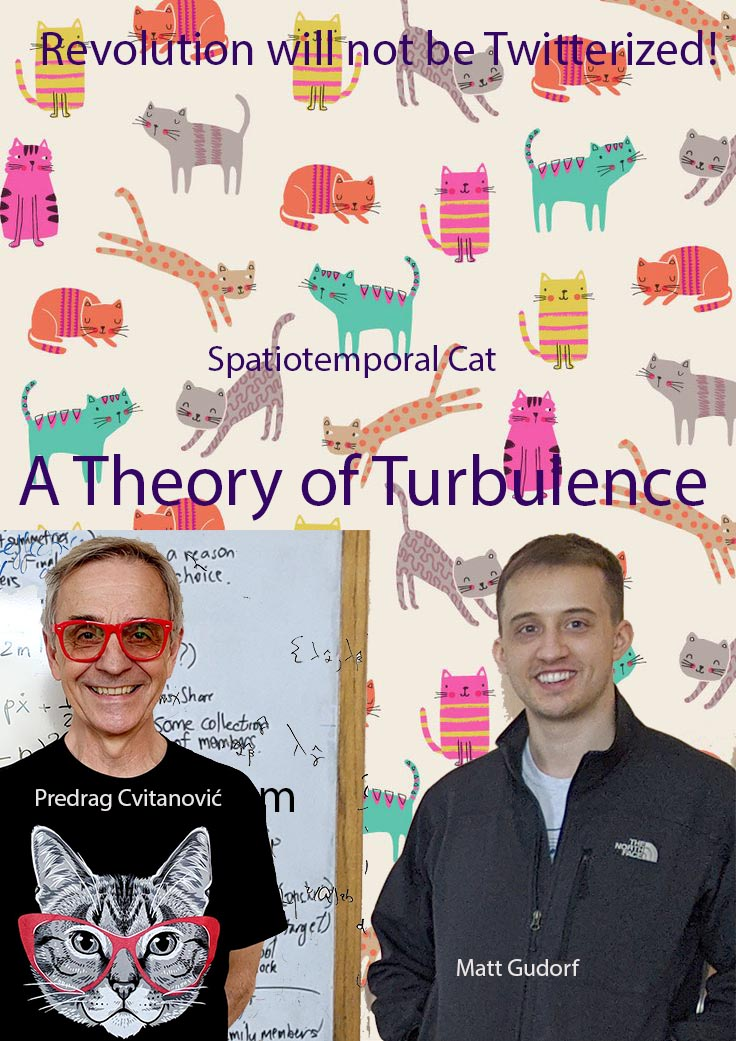
\includegraphics[width=0.55\textwidth]{HoweyCats}
%\end{center}
\end{frame}


\begin{frame}
  \titlepage
\end{frame}


\section[what this work is about]
 {what this work is about}

\begin{frame}{overview}
\begin{enumerate}
              \item {\Large
what this talk is about
                  }\textcolor{gray}{\small
              \item
turbulence in large domains
              \item
space is time
              \item
bye bye, dynamics
                    }
            \end{enumerate}
\end{frame}

\begin{frame}{how do clouds solve PDEs?}

\vfill

do clouds \textcolor{red}{integrate} Navier-Stokes equations?

\begin{center}
\centerline{\textcolor{red}{\Huge ?}}
%\end{center}
%for weather prediction, we store sets of weather sequences
%\bigskip\bigskip

%\begin{center}
\begin{minipage}[t]{\textwidth}
	\begin{center}
%\vspace{2ex}
\centerline{
\raisebox{-4.0ex}[5.5ex][4.5ex]
		 {
\includegraphics[height=12ex]{Hopf-a}}
~~~ $\Longrightarrow$ ~~ {other swirls} ~~ $\Longrightarrow$ ~~~
	\raisebox{-4.0ex}[5.5ex][4.5ex]
		 {
\includegraphics[height=12ex]{Hopf-b}}
          }
	\end{center}
\end{minipage}
\end{center}

are clouds Navier-Stokes supercomputers in the sky?

\end{frame}

\begin{frame}{part 1}
\begin{enumerate}
              \item {\Large
turbulence in large domains
                  }\textcolor{gray}{\small
              \item
space is time
              \item
spacetime
              \item
bye bye, dynamics
                    }
            \end{enumerate}
\end{frame}


\begin{frame}{goal : enumerate the building blocks of turbulence}
\begin{block}{Navier-Stokes equations} % (1822)}
\[
\dfrac{\partial \bv}{\partial t} + (\bv \cdot \nabla) \bv
	\,=\,
\frac{1}{R} \nabla ^2 \bv
-\nabla p
+ \mathbf{f}
    \,,\qquad
\nabla \cdot \bv = 0,
\]
\end{block}

\hfill{\small
velocity field  $\bv \in \mathbb{R}^3$
;
pressure field $p$
;
driving force $\mathbf{f}$
        }

\medskip

\begin{block}{describe turbulence}
starting from the equations (no statistical assumptions)
\end{block}

\bigskip

% large Reynolds number $R$:
\hfill {\Large\textcolor{red}{}}

\end{frame}

\begin{frame}{challenge : experiments are amazing}
\begin{center}
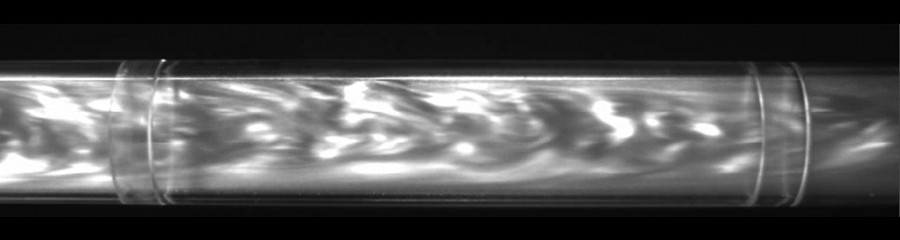
\includegraphics[width=0.7\textwidth]{mullin_puff2200} %pipe}
\end{center}
T. Mullin lab
\begin{center}
\bigskip
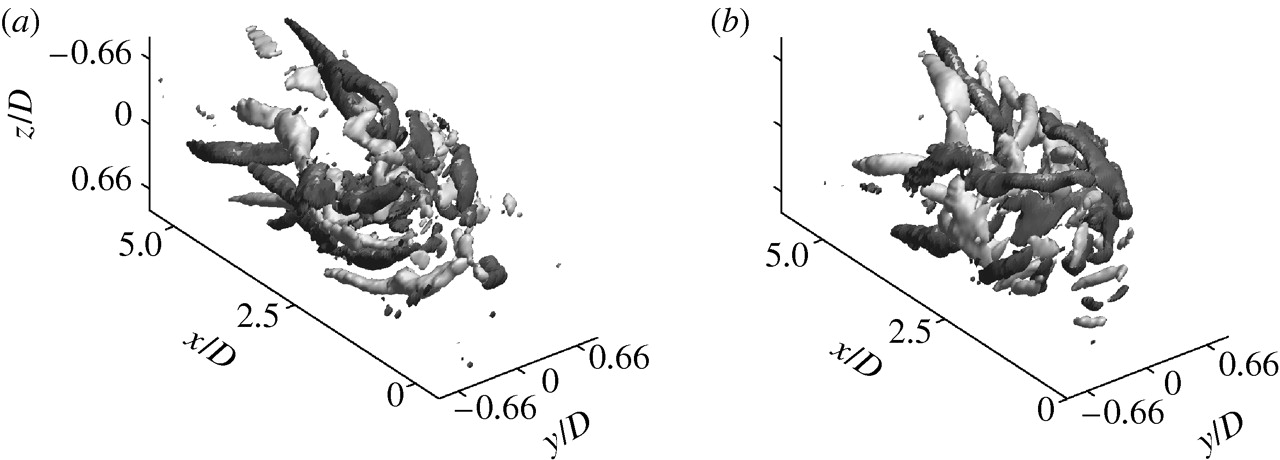
\includegraphics[width=0.7\textwidth]{deLHof09fig6} %pipe}
\end{center}
B. Hof lab
\end{frame}

%\begin{frame}{pipe theory and numerics}
%	\begin{columns}[t]
%	\column{.55\textwidth}
%amazing experiments! \\ amazing numerics! \\ beautiful visualizations !
%
%\bigskip\bigskip
%
%%relative periodic orbits,
%``Exact Coherent Structures'' :
%\\ numerical Navier-Stokes
%
%\medskip
%isosurfaces and cross sections \\ of the streamwise velocity
%
%\medskip
%
%\textcolor{red}{red} (\textcolor{blue}{blue}) streaks
%\\ are \textcolor{red}{faster} (\textcolor{blue}{slower}) \\ than the base flow
%
%\bigskip
%
%{{\tiny Ritter et al., Phys. Rev. Fluids (2018)}}
%
%	\column{.45\textwidth}
%\begin{center}
%  \includegraphics[width=1.0\textwidth,clip=true]
%                    {RZSEA18Fig3}
%\end{center}
%	\end{columns}
%\end{frame}

\section[dynamics in $\infty$ dimensions]
{dynamics in $\infty$ dimensions}

\begin{frame}{can simulate {\Huge large} computational domains}
\begin{center}
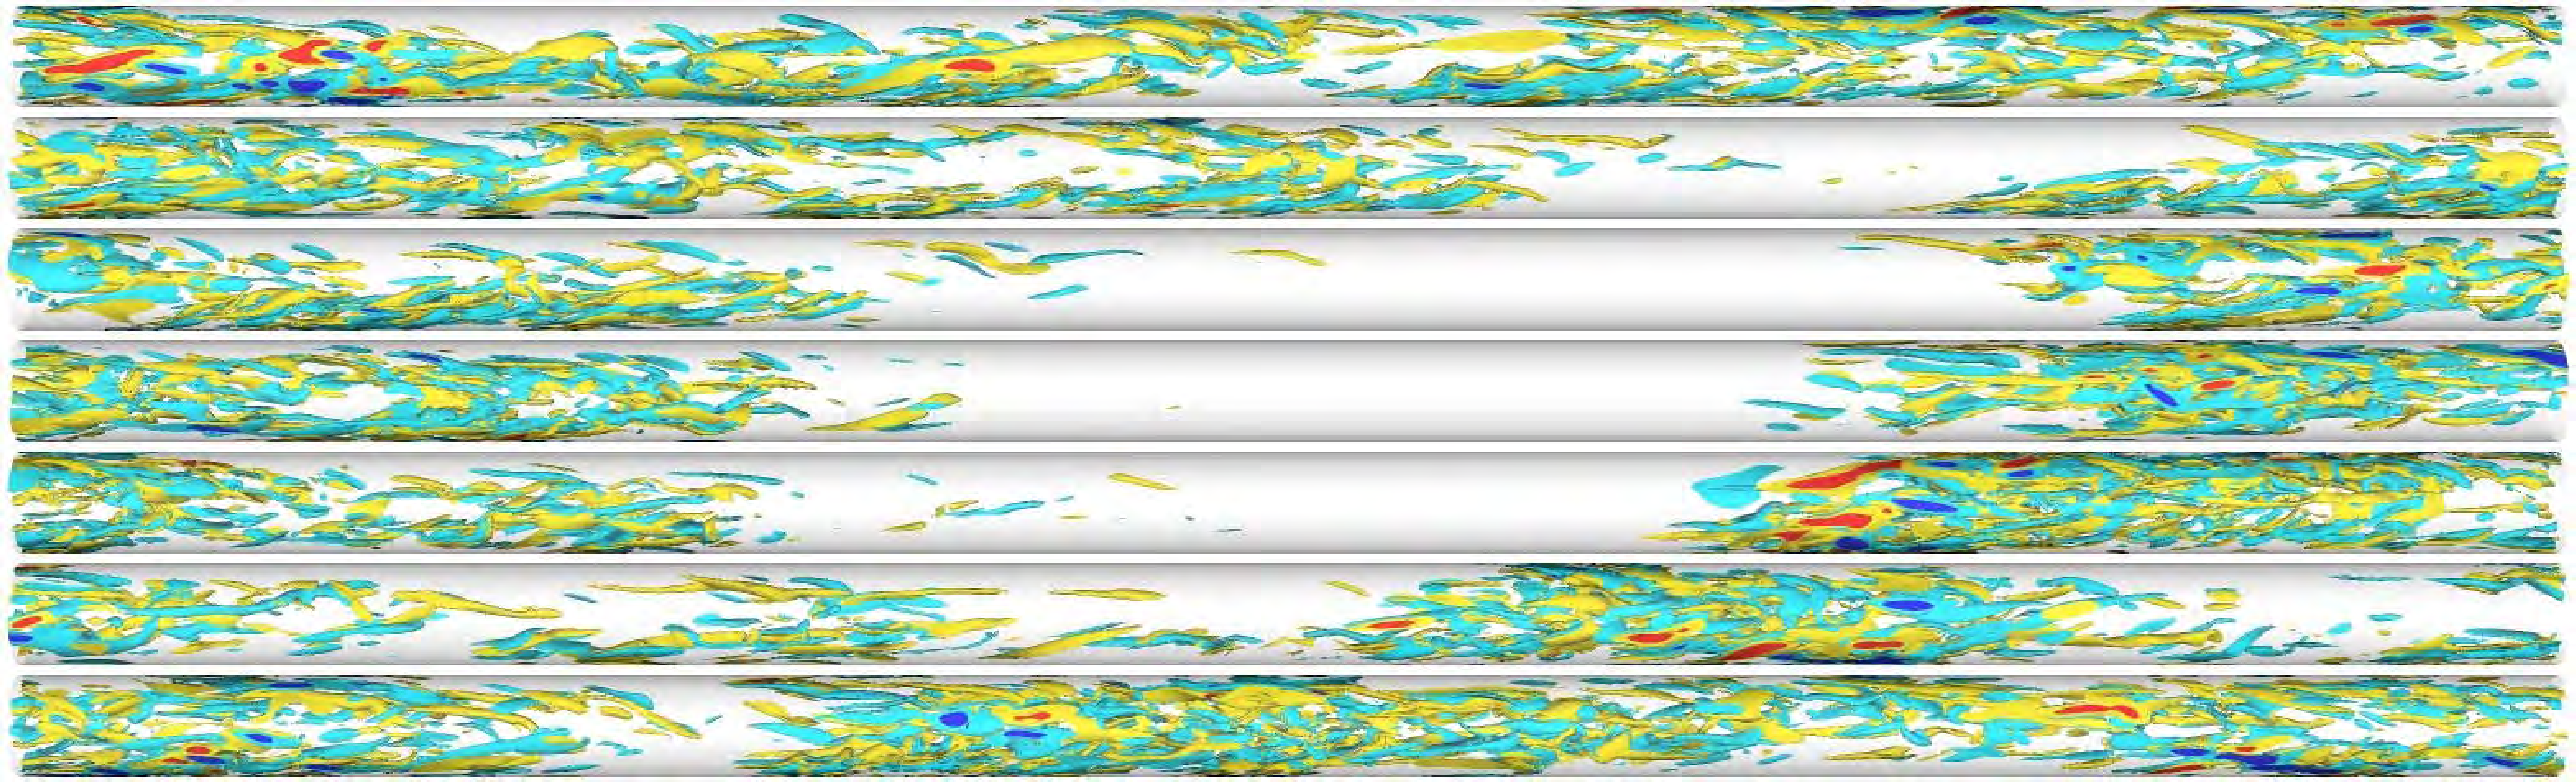
\includegraphics[width=1.0\textwidth]{AviHof13fig4}
\end{center}
pipe flow close to onset of turbulence
\footnote{M.~Avila and B.~Hof, {Phys. Rev. \bf E 87} (2013)}

\bigskip

but we have \textcolor{red}{\Huge hit a wall} :

\hfill exact coherent structures are too unstable to compute
\end{frame}

\begin{frame}{goal : we can do 3D turbulence, but for this presentation}
\begin{block}{Navier-Stokes equations} % (1822)}
\[
\dfrac{\partial \bv}{\partial t} + (\bv \cdot \nabla) \bv
	\,=\,
\frac{1}{R} \nabla ^2 \bv + (\cdots)
% -\nabla p + \mathbf{f}
%    \,,\qquad
%\nabla \cdot \bv = 0,
\]
\end{block}

\hfill{\small velocity field  $\bv(\bx;t) \in \mathbb{R}^3$}

\medskip

\begin{block}{not helpful for developing intuition}
we cannot visualize 3D velocity field at every 3D spatial point
\end{block}

\bigskip

% large Reynolds number $R$:
\hfill {\Large\textcolor{red}{look instead at 1D `flame fronts'}}
\end{frame}

\begin{frame}{(1+1) spacetime dimensional ``Navier-Stokes''}
\begin{block}{Navier-Stokes equations \hfill (1822)}
\[
\dfrac{\partial \bv}{\partial t} + (\bv \cdot \nabla) \bv
	\,=\,
\frac{1}{R} \nabla ^2 \bv + (\cdots)
\]
\end{block}
    \centerline{\textcolor{red}{$\blacktriangledown$}}
    \centerline{\textcolor{red}{$\blacktriangledown$}}
    \centerline{\textcolor{red}{$\blacktriangledown$}}
\begin{block}{\KS\ (1+1)\dmn\ PDE \hfill (1975)}
\[
  u_t + u \triangledown u \,=\,
    {\color{red}-}\triangledown^2 u {\color{red}-\triangledown^4 u}
    \,,\qquad   x \in \mathbb{R}
    \,,
\]
\end{block}
\bigskip

describes spatially extended systems such as
\begin{itemize}
 \item flame fronts in combustion
 \item reaction-diffusion systems
 \item \ldots
\end{itemize}
\end{frame}

\begin{frame}{an example : \KS\ on a large domain}
\begin{center}
  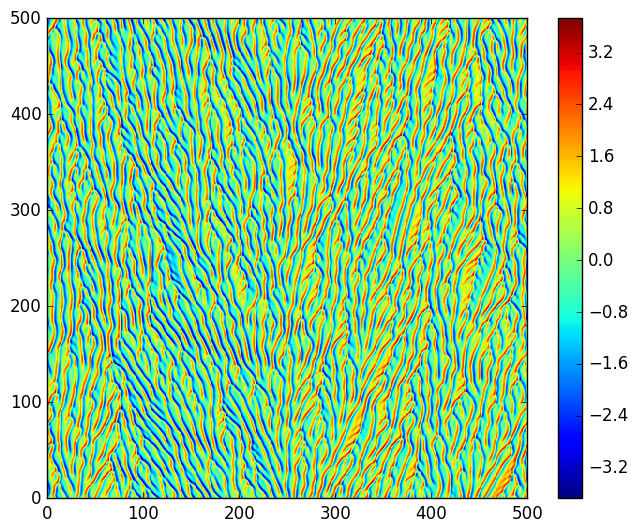
\includegraphics[width=.6\textwidth]{MNG_uu500b500}
%  \includegraphics[width=0.6\textwidth] %,height=0.5\textheight,clip=true]
%  {ks_largeL_cbar_200} %{ksevol-fig} %{ks_largeL_cbar}
\end{center}

{\footnotesize
[horizontal] space $\ssp \in [0,L]$
\qquad
{[up]} time evolution
}

\begin{itemize}
\item turbulent behavior
\item simpler physical, mathematical and computational setting than Navier-Stokes
\end{itemize}
\end{frame}

\begin{frame}{another example of large spacetime domain simulation}
\begin{block}{complex Ginzburg-Landau}
  \includegraphics[width=0.515\textwidth] %,height=0.5\textheight,clip=true]
  {cGLdefturbabs}
  \hfill
  (will return to this)
\end{block}

{\footnotesize
[horizontal] space $\ssp \in [-L/2,L/2]$
\qquad
{[up]} time evolution
}

\hfill {\scriptsize \color{orange} codeinthehole.com/static/tutorial/coherent.html}
\end{frame}

\begin{frame}{compact space, infinite time cylinder}
\begin{center}
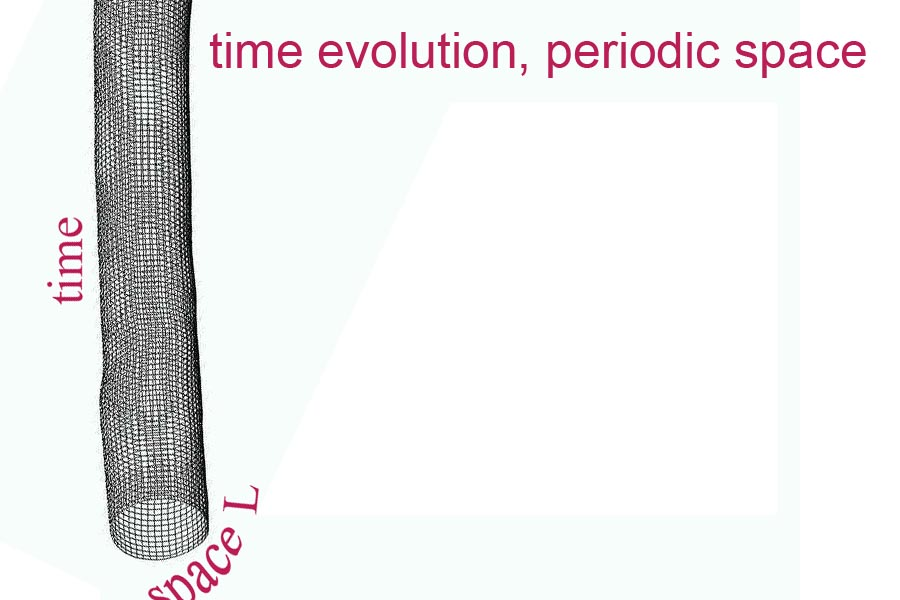
\includegraphics[width=0.9\textwidth]{cylinderTime}
\end{center}
% \hfill \color{red}{(impossible without xxx)}
so far : Navier-Stokes on compact spatial domains, all times
\end{frame}

\begin{frame}{compact space, infinite time} % \KS}
\begin{block}{\KS\ equation}
\[
  u_t \,=\,
    -({\color{red}+}\triangledown^2 +{\color{red}\triangledown^4}) u
    - u \triangledown u
    \,,\qquad   x \in [-L/2,L/2]
    \,,
\]
\end{block}

\bigskip

\begin{block}{in terms of discrete spatial Fourier modes}
$N$ ordinary differential equations (ODEs) in time
\[
\dot{\Fu}_k(\zeit) = ( q_k^2 - q_k^4 )\, \Fu_k(\zeit)
- i \frac{q_k}{2} \!\sum_{k'=0}^{N-1} \!\!\Fu_{k'}(\zeit) \Fu_{k-k'}(\zeit)
\,.
%\label{e-Fks}
\]
\end{block}
\end{frame}


\subsection{types of solutions}
\begin{frame}{evolution of \KS\ on small $L=22$ cell}
\begin{center}
  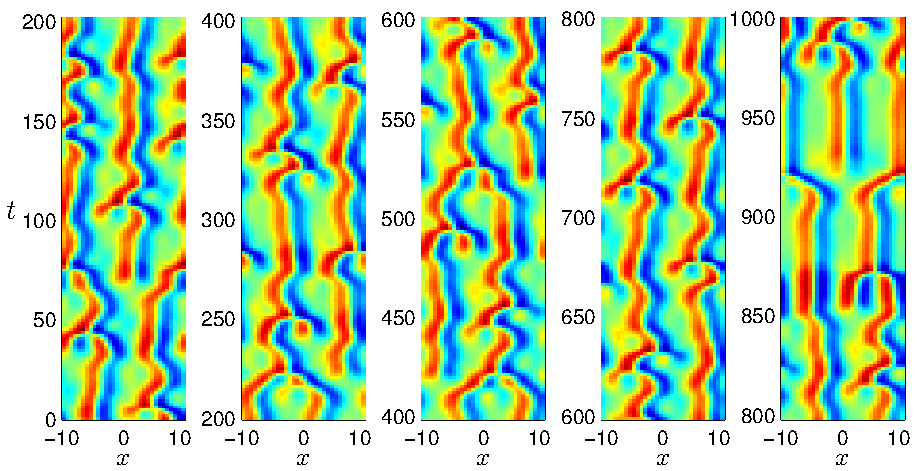
\includegraphics[width=0.9\textwidth,clip=true]{ks_L22_long_orbit}
\end{center}
horizontal: $x \in [-11,11]$
\\
vertical: time
\\
color: magnitude of $u(x,t)$
\end{frame}

\begin{frame}{part 2}
\begin{enumerate}
              \item
    \textcolor{gray}{\small
turbulence in large domains
        }
              \item
    {\Large
space is time
    }\textcolor{gray}{\small
              \item
spacetime
              \item
bye bye, dynamics
                    }
            \end{enumerate}
\end{frame}

\begin{frame}{yes, but}
\begin{center}
{\huge is space time?}
\end{center}
\end{frame}

\begin{frame}{compact time, infinite space}
rewrite \KS
\bea
    u_\zeit &=&  - u u_\conf
    -u_{\conf \conf}-u_{\conf \conf \conf \conf}
\nonumber     % \label{e-ks}
\eea
 as  4-fields vector
\bea
\transp{{\bf u}}&=&(u,u^{'},u^{''},u^{'''})
    \continue
&& \mbox{where }
    u^{'}   \equiv u_{\conf} \,,\;
    u^{''}  \equiv u_{\conf \conf} \,,\;
    u^{'''} \equiv u_{\conf \conf \conf}
\nnu
\eea
equation
\(
\frac{d~}{d\conf}{\bf u}(x)={\bf v}(x)
\)
now {\color{blue}1st order} in {\color{blue}spatial} derivative
\begin{block}{\KS\ = four coupled 1st order PDEs}
\bea
    \frac{d\,u}{d\conf}       &=& u^{'}
\,,\qquad
    \frac{d\,u^{'}}{d\conf}   \,=\,   u^{''}
\continue
    \frac{d\,u^{''}}{d\conf~}   &=&   u^{'''}
\,,\qquad
    \frac{d\,u^{'''}}{d\conf~~}  \,=\,  - u_{\zeit} - u^{''} - u\,u^{'}
\nonumber
\eea
\end{block}
\end{frame}

\begin{frame}{compact time, infinite space}
  1st order in {\color{blue}spatial} derivative
\begin{block}{evolve four 1st order PDEs for ${\bf u}(x)$ in $\conf$,}
\begin{itemize}
  \item
\[
\frac{d~}{d\conf}{\bf u}(x)={\bf v}(x)
\]
  \item
compact in time, periodic boundary condition
\[
  u(\conf, \zeit) = u(\conf, \zeit + \period{})
\]
  \item
initial data
\[
  \transp{{\bf u}}_0=(u(\conf_0, \zeit),u^{'}( \conf_0, \zeit),
                      u^{''}( \conf_0, \zeit),u^{''}( \conf_0, \zeit))
\]
specified for all $\zeit \in [0, \period{})$, at a fixed space point $\conf_0$
\end{itemize}
\end{block}
\end{frame}

\begin{frame}{can do : compact time, infinite space cylinder}
\begin{center}
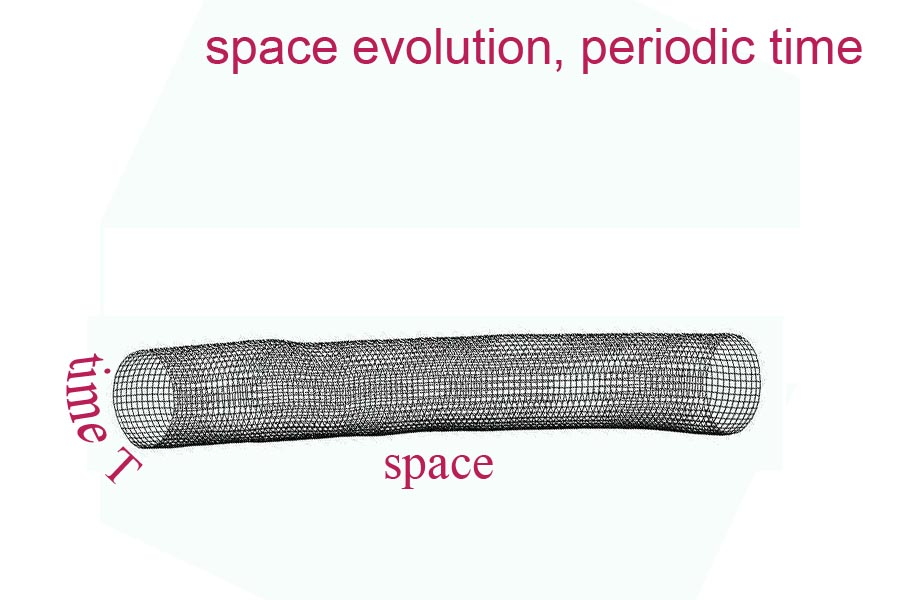
\includegraphics[width=0.9\textwidth]{cylinderSpace}
\end{center}
% \hfill \color{red}{(impossible without xxx)}
\end{frame}

\begin{frame}{a time-invariant \eqv, spatial \po}
\begin{center}
  \begin{minipage}[height=.45\textheight]{.45\textwidth}
    \centering \small{\texttt{(left)}}
    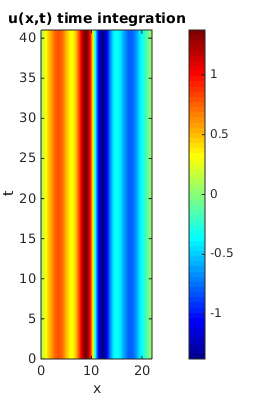
\includegraphics[width=\textwidth,height=.45\textheight]{MNGeq1time}
  \end{minipage}
  \begin{minipage}[height=.45\textheight]{.45\textwidth}
    \centering \small{\texttt{(right)}}
    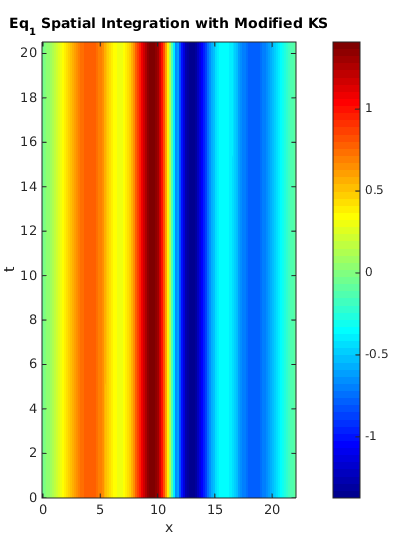
\includegraphics[width=\textwidth,height=.45\textheight]{MNGeq1space}
  \end{minipage}
\end{center}
   %\caption{
  evolution of $\EQV{1}$ : (left) in time, (right) in space
   \\
   initial condition for the spatial integration is the time strip
   $u(\conf_0,\zeit)$, $\zeit = [0,\period{})$, where time period
   $\period{} =0$, spatial $x$ period is $L=22$.
   % }\label{fig:MNGeqva1spttmp}

\vfill\hfill        Michelson 1986
%, Gudorf 2016
\end{frame}

\begin{frame}{a spacetime \twot\ integrated in either time or space}
\begin{center}
  \begin{minipage}[height=.40\textheight]{.35\textwidth}
    \centering \small{\texttt{(left)}}
    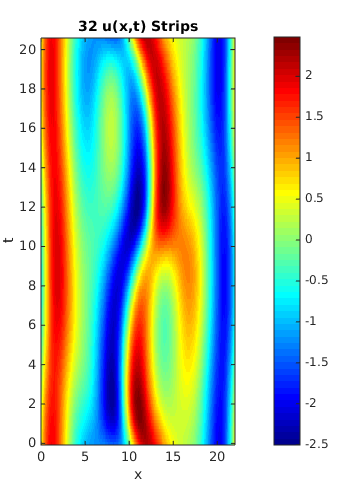
\includegraphics[width=\textwidth,height=.60\textheight]{MNGcomp32xint22}
  \end{minipage}
~~~~~~~~~
  \begin{minipage}[height=.40\textheight]{.35\textwidth}
    \centering \small{\texttt{(right)}}
    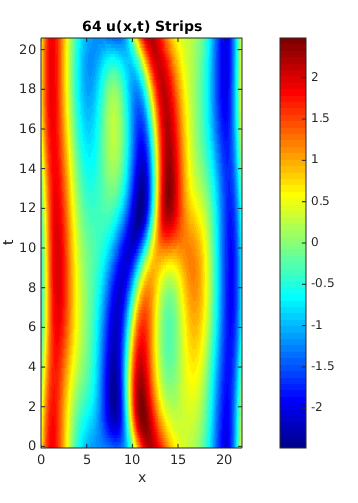
\includegraphics[width=\textwidth,height=.60\textheight]{MNGcomp64xint22}
  \end{minipage}
\end{center}
    (left) old : time evolution. (right) new : space evolution
    \\
    $x=[0,L]$ %22]$,
       initial condition : time periodic line $t = [0,T]$
  %2\,T_{\PPO{10.2}})$
  %\label{fig:MNGcompxint2}

\vfill\hfill        Gudorf 2016
\end{frame}

\begin{frame}{but integrations are uncontrollably unstable}

\begin{center}
{\huge neither} time {\huge nor} space integration {\huge works} \\
for large domains
\end{center}

\vfill
\color{red}{rethink the calculation}
\end{frame}

%%%%%%%%%%%%%%%%%%%%%%%%%%%%%%%%%%%%%%%%%%%%%%%%%%%%%%%%%%%%%%%%%%%%%%%%%%%
\begin{frame}{part 3}
\begin{enumerate}
              \item
    \textcolor{gray}{\small
turbulence in large domains
              \item
space is time
    }
              \item {\Large
spacetime
    }\textcolor{gray}{\small
              \item
bye bye, dynamics
                    }
            \end{enumerate}
\end{frame}

\begin{frame}{complex Ginzburg-Landau on a large spacetime domain}
\begin{block}{goal : enumerate nearly recurrent chronotopes}
  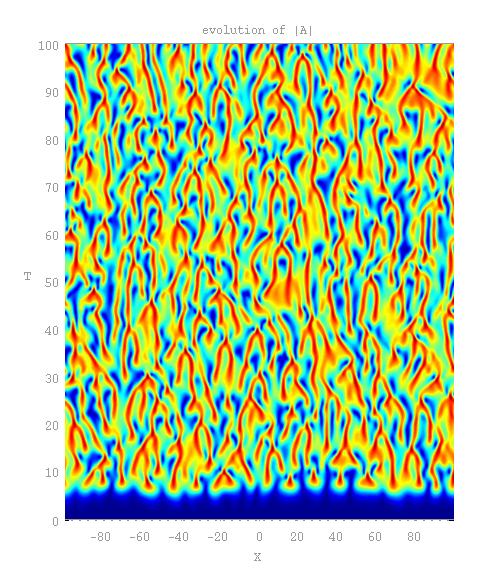
\includegraphics[width=0.4635\textwidth]{cGLdefturbabs}%
~~\raisebox{+3.33ex}[5.5ex][4.5ex]
		 {
\includegraphics[width=0.36\textwidth]{cGLdefturbclip}}
\end{block}

{\footnotesize
[left-right] space $\ssp \in [-L/2,L/2]$
\qquad
{[up]} time $t\in [0,\period{}]$
}
\end{frame}

\begin{frame}
    \frametitle{\KS\ on a large spacetime domain}
\begin{block}{the same small tile recurs often in a turbulent pattern}
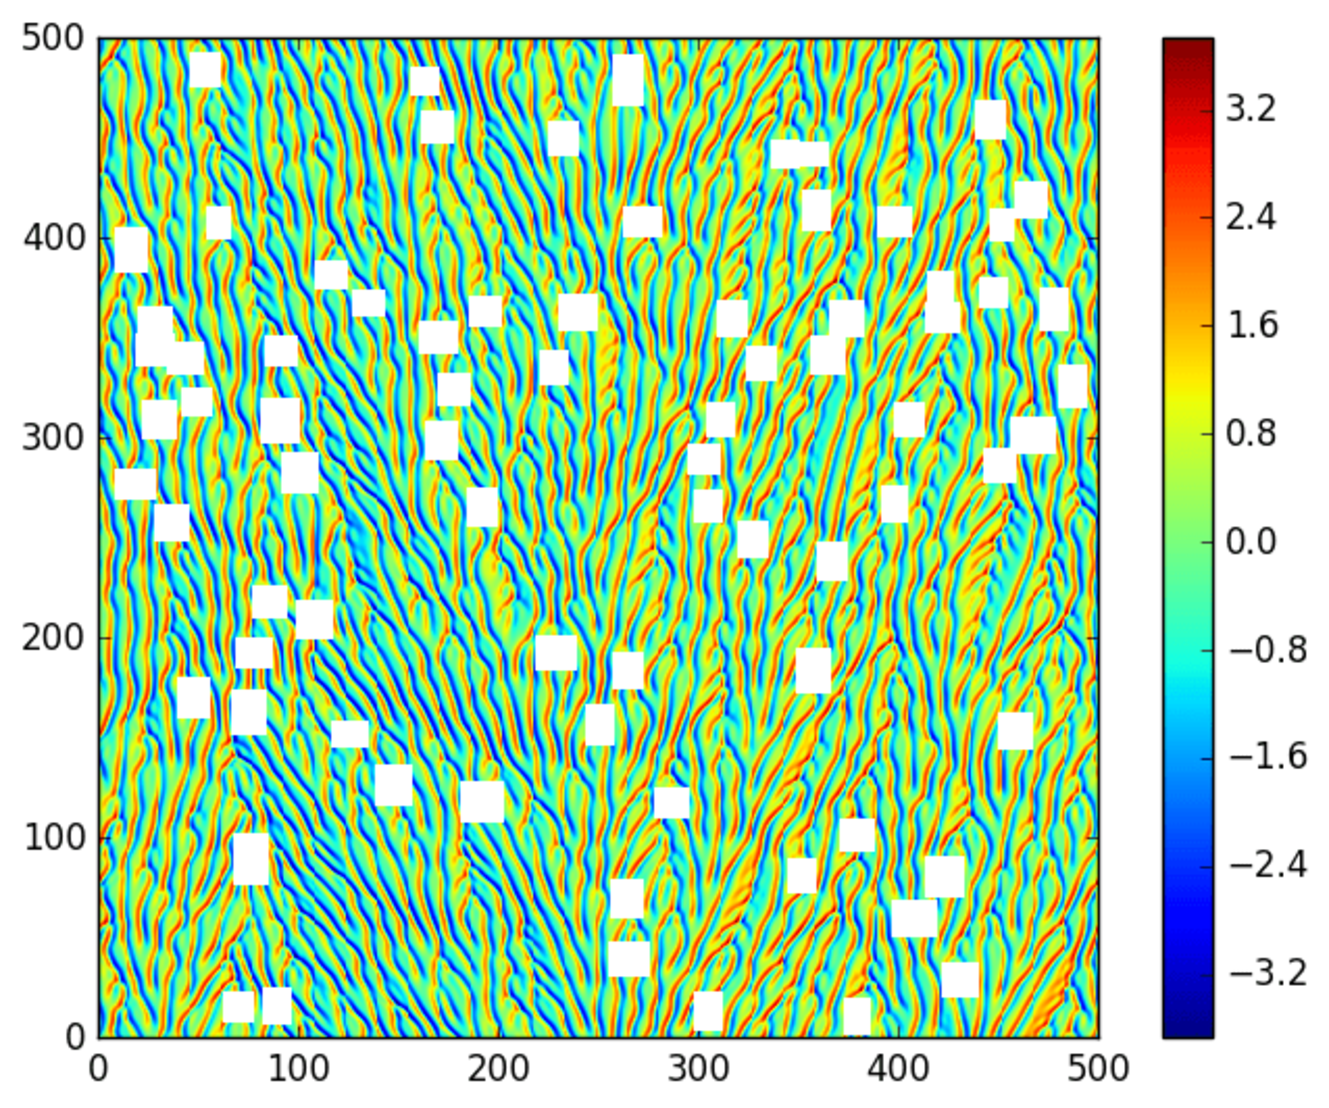
\includegraphics[width=.48\textwidth]{MNG_uu500b500co}
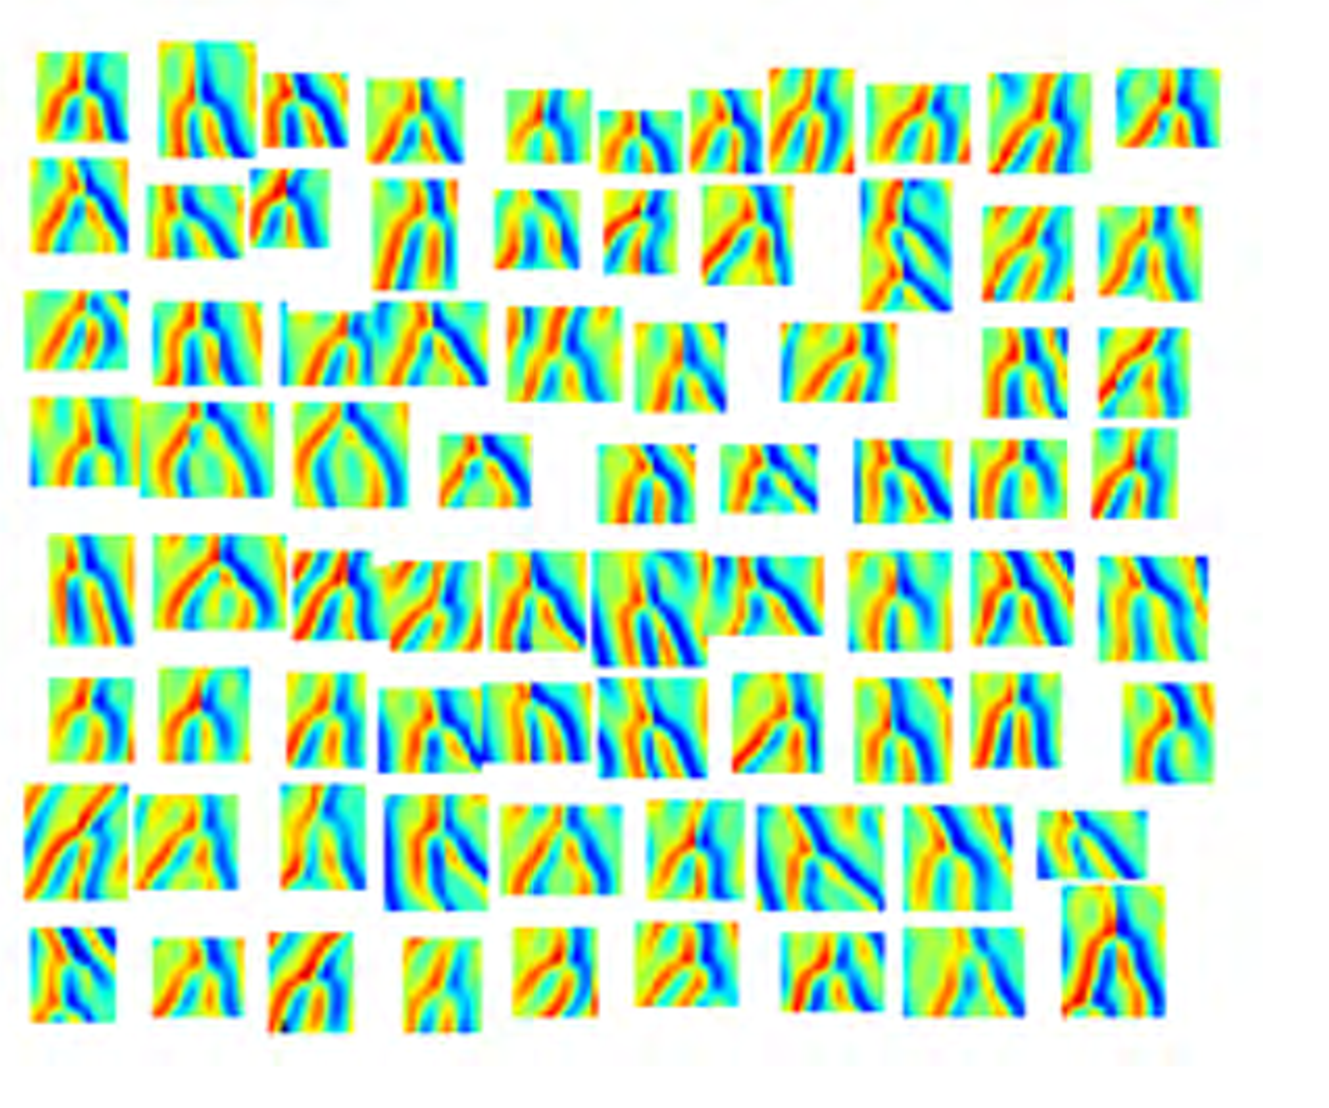
\includegraphics[width=.48\textwidth]{cutouts}
\end{block}
goal : define, enumerate nearly recurrent tiles
\end{frame}

\begin{frame}{chronotope
    \footfullcite{LePoTo96}%$^,$\footfullcite{WK09}
}
\begin{bartlett}{
In literary theory and philosophy of language, the chronotope is how
configurations of time and space are represented in language and
discourse.
                }\bauthor{
\HREF{https://en.wikipedia.org/wiki/Chronotope}
{Wikipedia : Chronotope}
                }
\end{bartlett}

\bigskip
\bigskip
%goes without saying : was done by a Soviet scientist first

\begin{itemize}
  \item Mikhail Mikhailovich Bakhtin (1937)
%  \item Politi, Giacomelli, Lepri, Torcini (1996)
%  \item Gutkin and Osipov (2016)
\end{itemize}
\end{frame}

\begin{frame}{use spatiotemporally compact solutions as chronotopes}
\begin{center}
\includegraphics[width=0.9\textwidth]{torusSpTime}
\end{center}
this `exact coherent structure'\\
\textcolor{red}{shadows} a small patch of spacetime solution $u( \conf, \zeit)$
\end{frame}

\begin{frame}{\po s generalize to $d$-tori}

\begin{block}{1 time, 0 space dimensions}
a {\statesp} point is {\em periodic} if its orbit returns to it
after a finite time \period{} ;
\\
such orbit tiles the time axis
by infinitely many repeats
\end{block}

\bigskip

\begin{block}{1 time, $d$-1 space dimensions}
 a {\statesp} point is {\em spatiotemporally periodic} if
it belongs to \\ an invariant $d$-torus ${\R}$ ;
\\
such torus tiles the spacetime
by infinitely many repeats
%,\\
%\ie, a \brick\ $\Mm_{\R}$ that
%tiles the lattice state  $\Mm$, \\
%with period $\ell_j$ in $j$th lattice direction
\end{block}
\end{frame}

\begin{frame}{a spacetime \twot\ integrated in either time or space}
\begin{center}
  \begin{minipage}[height=.40\textheight]{.35\textwidth}
    \centering \small{\texttt{(left)}}
    \includegraphics[width=\textwidth,height=.60\textheight]{MNGcomp32xint22}
  \end{minipage}
~~~~~~~~~
  \begin{minipage}[height=.40\textheight]{.35\textwidth}
    \centering \small{\texttt{(right)}}
    \includegraphics[width=\textwidth,height=.60\textheight]{MNGcomp64xint22}
  \end{minipage}
\end{center}
    (left) ~~~old : time evolution
    ~~~~~$t=[0,\period{}]$ %22]$,
        \\ \hfill {\scriptsize
       initial condition : space periodic line $x = [0,\speriod{}]$
                  }
        \\
    (right) new : space evolution
    $x = [0,\speriod{}]$ %22]$,
        \\ \hfill {\scriptsize
       initial condition : time periodic line $t = [0,\period{}]$
                  }
  %2\,T_{\PPO{10.2}})$
  %\label{fig:MNGcompxint2}

\vfill\hfill        Gudorf 2016
\end{frame}

\begin{frame}{every compact solution is a fixed point on a discrete lattice}
discretize $u_{nm} = u(\conf_n,\zeit_m)$ over
$N M$ points of spatiotemporal periodic lattice $\conf_n = n L/N$,
 $\zeit_m = m \period{}/M$, Fourier transform :
\[
\Fu_{k\ell} \,=\,
  \frac{1}{NM} \sum^{N-1}_{n=0} \sum^{M-1}_{m=0}
  u_{nm} \, e^{-i(q_k\conf_n + \omega_\ell \zeit_m)}
    \,,\quad
q_k = \frac{2 \pi k}{L}
    \,,\;
\omega_\ell = \frac{2 \pi \ell}{\period{}}
% \label{spattempFT}
\]
\KS\ is no more a PDE, \\
but an {\color{blue}{algebraic}} $[N\!\times\!M]$\dmn\ problem\\
of determining {\color{blue}{global}} solution ${\bf u}$ to
\begin{block}{fixed point condition}
\[
\left(- i \omega_\ell - ( q_k^2 - q_k^4 ) \right)\Fu_{k\ell}
+ i \frac{q_k}{2} \!\sum_{k'=0}^{N-1} \sum^{M-1}_{m'=0}\!\!
\Fu_{k'm'} \Fu_{k-k',m-m'}
    = 0
\]
\end{block}
\end{frame}

\begin{frame}{every calculation is a spatiotemporal lattice calculation}
field is discretized as
$\Fu_{k\ell}$ values  \\ over
$N M$ points of a periodic lattice

%\medskip

\begin{center}
\includegraphics[width=0.9\textwidth]{torusSpTime}
\end{center}
% \hfill \color{red}{(impossible without xxx)}
\end{frame}

\begin{frame}{professor Zweistein forgets to take his meds}
\medskip
statement : {\huge HA!} \\
You are imposing by hand the space \& time periods
\speriod{}, \period{} {\huge !}

\begin{center}
\includegraphics[width=0.35\textwidth]{spaceTime1}
\end{center}

answer : {\huge\color{red}{NO!}} \\
nature chooses \speriod{} \& \period{},
they are free parameters.
\end{frame}

\begin{frame}{there is no more time evolution}
solution to \KS\ is now given as
\begin{block}{condition that}
at each lattice point $k\ell$ \\
the tangent field at $\Fu_{k\ell}$
\end{block}
satisfies the equations of motion
\[
\left[- i \omega_\ell - ( q_k^2 - q_k^4 ) \right]\Fu_{k\ell}
+ i \frac{q_k}{2} \!\sum_{k'=0}^{N-1} \sum^{M-1}_{m'=0}\!\!
\Fu_{k'm'} \Fu_{k-k',m-m'}
    =
0
%\,.
%\label{e-FksSpattemp}
\]

\bigskip

this is a \textcolor{red}{local} tangent field constraint on a \textcolor{red}{global} solution
\end{frame}

\begin{frame}{think globally, act locally}
    \begin{center}
\includegraphics[width=0.85\textwidth]{globalLocal}
    \end{center}
for each symbol array \Mm, a periodic lattice state $\Xx_\Mm$
\end{frame}

\begin{frame}{unexpected gift from nature}
robust : no exponential instabilities
\\
\hfill as there are no finite time / space integrations
\bigskip

no need for $\sim
10^{-11}$ accuracies,
\bigskip

{\huge \textcolor{red}{so}}
\bigskip

accuracy to a few \% suffices, \\
\hfill you only need to get the shape of a solution right
\end{frame}

\begin{frame}{part 4}
\begin{enumerate}
              \item
    \textcolor{gray}{\small
turbulence in large domains
              \item
space is time
              \item
spacetime    }
              \item {\Large
spacetime computations
    }\textcolor{gray}{\small
              \item
bye bye, dynamics
                    }
            \end{enumerate}
\end{frame}


\begin{frame}{how to find solutions ? an ODE example}
\begin{center}
the law of motion : $\qquad \dot{\ssp} = \pVeloc(\ssp)$
\begin{minipage}[c]{0.55\textwidth}
\textcolor{red}{guess loop tangent}
$\lVeloc(\lSpace)
	\neq
\pVeloc(\lSpace)$

	\vskip 0.5cm

\textcolor{green}{periodic orbit}
$\lVeloc(\lSpace)$,~$\pVeloc(\lSpace)$
aligned
\end{minipage}%
~~~~~~~\begin{minipage}[c]{0.40\textwidth}
	\begin{center}
	\includegraphics[width=0.7\textwidth]{velocField}
	\end{center}
\end{minipage}
\end{center}
\begin{block}{cost function}%
\[
\costF[\lSpace] =
            \oint_\Loop ds\,(\lVeloc-\pVeloc)^2
    \,;\quad
    \lVeloc = \lVeloc(\lSpace(s,\tau))\,,\,\,
    \pVeloc = \pVeloc(\lSpace(s,\tau))
\,,
% \label{loopCostFct}
\]
\end{block}
\bigskip

penalize\footfullcite{lanVar1}%{ Lan and Cvitanovi\'c, Phys. Rev. (2004)}
 misorientation of the loop tangent
$\lVeloc(\lSpace)$
relative to the true dynamical flow tangent field $\pVeloc(\lSpace)$
\end{frame}

\begin{frame}{how do clouds solve PDEs?}
clouds do not \textcolor{red}{\Huge NOT} {integrate} Navier-Stokes equations

\bigskip\bigskip

\begin{center}
\begin{minipage}[t]{\textwidth}
	\begin{center}
\centerline{
\raisebox{-4.0ex}[5.5ex][4.5ex]
		 {\includegraphics[height=12ex]{Hopf-a}}
~~~ $\Longrightarrow$ ~~ {other swirls} ~~ $\Longrightarrow$ ~~~
	\raisebox{-4.0ex}[5.5ex][4.5ex]
		 {\includegraphics[height=12ex]{Hopf-b}}
          }
	\end{center}
\end{minipage}
\end{center}

do clouds satisfy Navier-Stokes equations?

\bigskip

{\Large yes!}

\centerline{
\textcolor{blue}{they satisfy them \textcolor{red}{\large locally}, everywhere and at all times}
}
\end{frame}

\begin{frame}{the equations imposed as local constraints}
\begin{block}{\KSe}
\[
F(u) = u_t + u_{\conf \conf} + u_{\conf \conf \conf \conf} + u u_{\conf} = 0
\]
\end{block}
\bigskip\bigskip
for example, minimize over the entire 2-torus
\begin{block}{cost function}
\[
G \equiv \frac{1}{2} |F(u)|^2_{L \times T}
%\ee{costfunctional}
\]
\end{block}
\vfill\hfill\textcolor{red}{\Huge need your help !}
\end{frame}

\begin{frame}{adjoint descent}
cost function
\[
  G = \frac{1}{2} \mathbf{F}^{\top}\mathbf{F}
  \,.
\]
introduce fictitious time ($\tau$) flow by differentiation of cost function.
\[
  \partial_{\tau}G = (J^{\top}\mathbf{F})^{\top}(\partial_{\tau}\mathbf{x})
\]
  ``adjoint descent'' method defined by chosing\footfullcite{Faraz15}
\[
  \partial_{\tau}\mathbf{x} = -(J^{\top}\mathbf{F})
\]

\end{frame}

\begin{frame}{does it work at all ?}
add strong noise to a \emph{known} solution, \\ twice the typical amplitude
\begin{block}{only the first test}
{\scriptsize (not how we actually generate guesses)} \\
\begin{minipage}[height=.32\textheight]{.35\textwidth}
\centering %\small{\texttt{(a)}}
\includegraphics[width=\textwidth,height=.32\textheight]{MNG_ppo1_noise_init}
\end{minipage}
    \qquad
\begin{minipage}[height=.32\textheight]{.35\textwidth}
\centering %\small{\texttt{(right)}}
\includegraphics[width=\textwidth,height=.32\textheight]{MNG_ppo1_noise_conv}
\end{minipage}
%\caption{ \label{fig:MNG_adjnewt_robustness}
\end{block}

{\scriptsize (left) initial guess: a known %\PPO{10.2}
\twot} \\
$(\speriod{0},\period{0})=(22.0,20.5057459345)$
+
strong random noise
\medskip

{\scriptsize (right) the resulting adjoint descent converged \twot} \\
$(\speriod{f},\period{f})=(21.95034935834641,20.47026321555662)$
%\end{figure}
\end{frame}

\begin{frame}{initial guess generation ?}
 \textcolor{blue}{the time scale} : the shortest
`turnover' scale characterized by the period of the shortest \po? Or perhaps
the Lyapunov time?

\bigskip

\textcolor{blue}{the spatial scale} :
$\bar{L}=2\pi\sqrt{2}$, the  most unstable spatial wavelength of the \KS

\bigskip

%%%%%%%%%%%%%%%%%%%%%%%%%%%%%%%%%%%%%%%%%%%%%%%%%%%%%%%%%%%%%%%%
%\label{fig:MNG_spacetime_smoothed} from siminos/spatiotemp/blogMNG.tex
\begin{minipage}[height=.32\textheight]{.30\textwidth}
\includegraphics[width=\textwidth,height=.32\textheight]{MNG_T100L44_init}
\end{minipage}

\medskip
initial : spatial $\bar{L}$-modulated random guess
%%%%%%%%%%%%%%%%%%%%%%%%%%%%%%%%%%%%%%%%%%%%%%%%%%%%%%%%%%%%%%%%

% \vfill\hfill        Gudorf 2018
\end{frame}

\begin{frame}{KS \twot\ found variationally}
%%%%%%%%%%%%%%%%%%%%%%%%%%%%%%%%%%%%%%%%%%%%%%%%%%%%%%%%%%%%%%%%
%\label{fig:MNG_spacetime_smoothed} from siminos/spatiotemp/blogMNG.tex
\begin{minipage}[height=.72\textheight]{.40\textwidth}
\centering \small{\texttt{(left)}}
\includegraphics[width=\textwidth,height=.63\textheight]{MNG_T100L44_init}
\end{minipage}
\begin{minipage}[height=.72\textheight]{.40\textwidth}
\centering \small{\texttt{(right)}}
\includegraphics[width=\textwidth,height=.63\textheight]{MNG_T100L44_final}
\end{minipage}

\vfill
(left) initial : $\bar{L}=2\pi\sqrt{2}$ spatially modulated ``noisy'' guess

(right) adjoint descent : converged \twot\
% \\
% spatial and time periods
% $L=24.07$, $T=31.86$
%%%%%%%%%%%%%%%%%%%%%%%%%%%%%%%%%%%%%%%%%%%%%%%%%%%%%%%%%%%%%%%%

\vfill\hfill        Gudorf 2018
\end{frame}


\begin{frame}{initial guesses, embedded in ergodic sea?}
\begin{block}{Historically, }
guesses extracted from close recurrences \\
observed in long turbulent simulations
\end{block}
\bigskip\bigskip
            \begin{enumerate}
              \item
inefficient, finds only the shortest, least unstable orbits%
\footfullcite{pchaot}$^,$\footfullcite{GHCW07}
              \item
can integrate only not far in time
            \end{enumerate}

\vfill\hfill\textcolor{red}{\huge need spatiotemporal guesses}
\end{frame}

\begin{frame}{guesses extracted from large spacetime domains}
\begin{minipage}[height=.45\textwidth]{.45\textwidth}
\centering %\small{\texttt{(a)}}
\includegraphics[width=\textwidth,height=.45\textheight]{MNGadjdescent500b500init}
\end{minipage}
\begin{minipage}[height=.45\textwidth]{.45\textwidth}
\centering %\small{\texttt{(b)}}
\includegraphics[width=\textwidth,height=.45\textheight]{MNGadjdescent500b500fin}
\end{minipage}
%\caption{ \label{fig:MNGlarge_adjointdescent}

(left) random initial state on
%\hfill
$(\speriod{},\period{})=(500,500)$

(right) adjoint descent $\to$ typical \KS\ state

\vfill\hfill
finite windows are our starting guesses for \twots
\end{frame}

\begin{frame}{another, much twittered : machine learning guesses}
``reservoir computing'' example\footfullcite{PHGLO18}

\bigskip

 \begin{columns}
 \column{0.35\textwidth}
~~~~~~\includegraphics[width=1\textwidth]{PHGLO18fig2}
 \column{0.65\textwidth}
 \begin{itemize}
 \item[(a)] data: \\ \KS\ simulation
 \item[(b)] reservoir computing prediction
 \item[(c)] two subtracted agree to \\
            $\sim 5$ Lyapunov times
 \end{itemize}
 \end{columns}
\vfill {\Large Q : \textcolor{red}{how would you learn this data?}}
\end{frame}

\begin{frame}{embarrassment of riches}
\begin{center}
{\huge what to do?}
\end{center}

\vfill

{\Large Matthew N. Gudorf}

\medskip

\hfill has 1\,000's of such \twots
\end{frame}


\begin{frame}{part 5}
\begin{enumerate}
              \item
    \textcolor{gray}{\small
turbulence in large domains
              \item
space is time
              \item
spacetime
    }
              \item {\Large
fundamental tiles
    }\textcolor{gray}{\small
              \item
bye bye, dynamics
                    }
            \end{enumerate}
\end{frame}


\begin{frame}{building blocks of turbulence}

how do we \textcolor{red}{recognize} a cloud?

\bigskip
\begin{center}
\centerline{\textcolor{red}{\Huge WATCH}}
%\end{center}
%for weather prediction, we store sets of weather sequences
%\bigskip\bigskip

%\begin{center}
\begin{minipage}[t]{\textwidth}
	\begin{center}
%\vspace{2ex}
\centerline{
\raisebox{-4.0ex}[5.5ex][4.5ex]
		 {\includegraphics[height=12ex]{Hopf-a}}
~~~ $\Longrightarrow$ ~~ {other swirls} ~~ $\Longrightarrow$ ~~~
	\raisebox{-4.0ex}[5.5ex][4.5ex]
		 {\includegraphics[height=12ex]{Hopf-b}}
          }
	\end{center}
\end{minipage}
\end{center}

\bigskip

{\Large by recurrent shapes!}

\vfill

\centerline{
\textcolor{blue}{so, construct an \textcolor{red}{\Large alphabet} of possible shapes}
}
\end{frame}

\begin{frame}{extracting a fundamental tile}
\begin{minipage}[height=.60\textheight]{.24\textheight}
\centering % \small{\texttt{(a)n}}
\includegraphics[width=.3\textheight,height=.55\textheight]{MNG_gapfull}
\end{minipage}
    $\quad\Rightarrow\;$
\begin{minipage}[height=.60\textheight]{.24\textheight}
\centering % \small{\texttt{(b)}}
\includegraphics[width=.3\textheight,height=.25\textheight]{MNG_gapsub1}
\end{minipage}
    $\quad\;\;\Rightarrow\;$
\begin{minipage}[height=.60\textheight]{.18\textheight}
\centering             % \small{\texttt{(c)}}
\includegraphics[width=0.20\textheight,height=.21\textheight]{ksstFigs/MNG_gap}
\end{minipage}
    $\;\Rightarrow\;$
\begin{minipage}[height=.60\textheight]{.12\textheight}
\centering % \small{\texttt{(d)}}
\includegraphics[width=0.17\textheight,height=.21\textheight]{MNG_gap_final}
\end{minipage}
%\label{fig:MNG_catseyefigs}

1) \twot\ %full\_L26.7\_T54.
    \\
2) \twot\ computed from initial guess cut out from 1)
    \\
3) ``gap" \twot, % po\_L17.3\_T15.3  %\reffig{fig:MNG_ppo_subdomains},
     initally cut out from 2)
     \\
4) the ``gap"  prime  \twot\ fundamental domain
\end{frame}

\begin{frame}%[allowframebreaks]
  \frametitle{a trial set of prime (rubber) tiles}
  \begin{block} {an alphabet of \KS\ fundamental tiles}
\begin{minipage}[height=.60\textheight]{.25\textheight}
\centering             % \small{\texttt{(c)}}
\includegraphics[width=0.26\textheight,height=.27\textheight]{ksstFigs/MNG_defect}
\end{minipage} \qquad
  % \includegraphics[width=.2\textwidth]{MNG_hook}
  % \includegraphics[width=.2\textwidth]{MNG_half}
\begin{minipage}[height=.60\textheight]{.25\textheight}
\centering     %{\footnotesize\texttt{\quad\quad Gap}}
\includegraphics[width=0.26\textheight,height=.27\textheight]{ksstFigs/MNG_gap}
\end{minipage} \qquad
\begin{minipage}[height=.60\textheight]{.25\textheight}
\centering             % \small{\texttt{(c)}}
\includegraphics[width=0.25\textheight,height=0.25\textheight]{ksstFigs/MNG_streak}
\end{minipage}
  \end{block}
\vfill
utilize also discrete symmetries : \\
spatial reflection, spatiotemporal shift-reflect,
$\cdots$
\end{frame}

\begin{frame}{\KS\ tiled by a small tile}
  \includegraphics[width=0.7\textwidth] %,height=0.5\textheight,clip=true]
  {MNG_tiling_rpo_13p02_T15}
  \vfill
tiling by relative periodic \twot\ \\ $(L,T)=(13.02,15)$
\end{frame}

\begin{frame}{spacetime tiled by a larger tile}
  \includegraphics[width=0.7\textwidth] %,height=0.5\textheight,clip=true]
  {MNG_tiling_rpo_L33p73_T35}
  \vfill
tiling by relative periodic \twot\ \\ $(L,T)=(33.73,35)$
\end{frame}

\begin{frame}{spacetime tiled by a tall tile}
  \includegraphics[width=0.7\textwidth] %,height=0.5\textheight,clip=true]
  {MNG_tiling_ppo_L55p83_T24}
  \vfill
tiling by shift-reflect \twot\ \\ $(L,T)=(55.83,24)$
\end{frame}

\begin{frame}{spacetime tiled by a larger tile}
  \includegraphics[width=0.7\textwidth] %,height=0.5\textheight,clip=true]
  {MNG_tiling_rpo_L32p0192_T51}
  \vfill
tiling by  relative periodic  \twot\ \\ $(L,T)=(32.02,51)$
\end{frame}

\begin{frame}{spacetime tiled by a larger tile}
  \includegraphics[width=0.7\textwidth] %,height=0.5\textheight,clip=true]
  {MNG_tiling_rpo_L44p48_T50}
  \vfill
tiling by  relative periodic  \twot\ \\ $(L,T)=(44.48,50)$
\end{frame}

\begin{frame}{any particular tiling looks nothing like turbulent \KS !}
  \includegraphics[width=0.7\textwidth] %,height=0.5\textheight,clip=true]
  {MNG_large_ergodic}

{\footnotesize
[horizontal] space $\ssp \in [-L/2,L/2]$
\qquad
{[up]} time evolution
}
\end{frame}

\begin{frame}{part 6}
\begin{enumerate}
              \item
    \textcolor{gray}{\small
turbulence in large domains
              \item
space is time
              \item
spacetime
              \item
fundamental tiles
    }
              \item {\Large
gluing tiles
    }\textcolor{gray}{\small
              \item
bye bye, dynamics
                    }
            \end{enumerate}
\end{frame}


\begin{frame}%[allowframebreaks]
  \frametitle{a qualitative tiling guess}
  \begin{block} {a tiling and the resulting solution}
  \qquad
\begin{minipage}[height=.80\textheight]{.25\textheight}
\centering             % \small{\texttt{(c)}}
  \qquad\qquad
\includegraphics[width=0.25\textheight,height=.36\textheight]{MNG_ppo_frankenstein}
\end{minipage} \quad\quad
\begin{minipage}[height=.80\textheight]{.25\textheight}
\centering      {\footnotesize\texttt{\quad\quad 2-torus}}
\includegraphics[width=0.35\textheight,height=.45\textheight]{MNG_ppo_L30_T44}
\end{minipage} \qquad\qquad
  \end{block}
\end{frame}

\begin{frame}{turbulence.zip : each solution has a unique symbolic name}
  \begin{block} {symbolic dynamics is 2\dmn!}
  \begin{center}
  \includegraphics[width=.25\textwidth,height=.4\textheight]{MNG_ppo_frankenstein}
~~~\includegraphics[width=.25\textwidth,height=.4\textheight]{MNG_approxsymbdyn}
~~~\includegraphics[width=.25\textwidth,height=.4\textheight]{MNG_approxsymbdyntrinary}
%  \includegraphics[width=.3\textwidth,height=.3\textheight]{MNG_ppo_L30_T44}
  \end{center}
  \end{block}
\begin{itemize}
 \item each symbol indicates a corresponding spatiotemporal tile
 \item these are ``rubber'' tiles
\end{itemize}
\end{frame}

%%%%%%%%%%%%%%%%%%%%%%%%%%%%%%%%%%%%%%%%%%%%%%%%%%%%%%%%%%%%%%%%
\begin{frame}{part 7}
\begin{enumerate}
              \item
    \textcolor{gray}{\small
turbulence in large domains
              \item
space is time
    }
              \item
    {\Large
bye bye, dynamics
    }
            \end{enumerate}
\end{frame}

\begin{frame}{in future there will be no future}
\begin{center}
{\huge goodbye}
\end{center}

\vfill

to long time and/or space integrators

\medskip

\hfill they never worked and could never work
\end{frame}

\begin{frame}{life outside of time}
\textcolor{red}{the trouble}:

forward time-integration codes too unstable

\bigskip
\bigskip

\textcolor{blue}{multishooting inspiration}:
 replace a guess that a  \textcolor{blue}{point} is on the periodic
orbit by a guess of the \textcolor{blue}{entire orbit}.

\bigskip

$\to$

\bigskip

spatio-temporally periodic solutions of classical field theories
can be found by \textcolor{blue}{variational methods}
\end{frame}

\begin{frame}{the equations solved as global optimization problems}
\begin{block}{impose the equations as local constraints}
\[
F(u) = u_t + u_{\conf \conf} + u_{\conf \conf \conf \conf} + u u_{\conf} = 0
\]
\end{block}
\bigskip\bigskip
minimize globally
\begin{block}{perhaps using cost function}
\[
G \equiv \frac{1}{2} |F(u)|^2_{L \times T}
%\ee{costfunctional}
\]
\end{block}
\end{frame}

\begin{frame}{can computers}

\vfill

{\Huge do this ?             }

\vfill
\end{frame}

\begin{frame}{the answer is}

\vfill

{\Huge
scalability
                  }

\vfill

%\hfill in the spirit of this workshop
\end{frame}

\begin{frame}{compute locally, adjust globally}
\begin{block}{Navier-Stokes codes}
\begin{itemize}
 \item
T. M. Schneider : developing a matrix-free variational Navier-Stokes code,
machine learning initial guesses
 \item
D. Lasagna and A. Sharma  : developing variational adjoint solvers to
find periodic orbits with long periods
 \item
Q. Wang : parallelizing {\color{red}spatiotemporal}
computation is FLOPs intensive, but more robust than
integration forward in time
\end{itemize}
\end{block}

\vfill\hfill
it's rocket science%
\footfullcite{Schneider19}$^,$%
\footfullcite{LaShMe18}$^,$%
\footfullcite{WGBGQ13}
%\footnote{{\tiny Q. Wang \etal,}\HREF{https://doi.org/10.1063/1.4819390}
%{\tiny\em Towards scalable parallel-in-time turbulent flow simulations},
%{\tiny Physics of Fluids (2013)}}
\end{frame}


\begin{frame}{
towards scalable parallel-in-time turbulent flow simulations
}
\begin{block}{future :}%
processor speed $\to$ limit

\medskip

number of cores $\to 10^6 \to \cdots$

\medskip
\end{block}

\emph{Wang et al (2013)
    \footfullcite{WGBGQ13}%$^,$\footfullcite{Ihara66}
    :} % Gomez, Blonigan, Gregory and Qian 2013 :}

next-generation : spacetime parallel
simulations, \\
on discretized $4D$ spacetime
computational domains, \\
with each computing core handling a spacetime lattice cell

\bigskip

compared to time-evolution solvers:
significantly higher level of concurrency, reduction the ratio of
inter-core communication to floating point operations

\bigskip

$\qquad\qquad\Rightarrow$ a path towards exascale DNS of turbulent flows
\end{frame}

\begin{frame}{enumerate hierarchically spatiotemporal patterns }
  \begin{block} {2D symbolic encoding $\Rightarrow$ admissible solutions}
  \begin{center}
\includegraphics[width=.25\textwidth,height=.38\textheight]{MNG_approxsymbdyntrinary}
~~~\includegraphics[width=.25\textwidth,height=.38\textheight]{MNG_ppo_frankenstein}
~~~\includegraphics[width=0.35\textheight,height=.45\textheight]{MNG_ppo_L30_T44}
  \end{center}
  \end{block}
\begin{itemize}
 \item each symbol indicates a minimal spatiotemporal tile
 \item glue them in all admissible ways
\end{itemize}
\end{frame}

\begin{frame}{machine learning will be needed}
``reservoir computing'' example\footfullcite{PHGLO18}
\bigskip

 \begin{columns}
 \column{0.35\textwidth}
~~~~~~\includegraphics[width=1\textwidth]{PHGLO18fig2}
 \column{0.65\textwidth}
 \begin{itemize}
 \item[(a)] data: \\ \KS\ simulation
 \item[(b)] reservoir computing prediction
 \item[(c)] two subtracted agree to \\
            $\sim 5$ Lyapunov times
 \end{itemize}
 \end{columns}
\vfill {\Large Q : \textcolor{red}{how would you learn this data?}}
\end{frame}

\begin{frame}{take home : clouds do not integrate PDEs}
%and do they care what PST hour is it?
%\\
%and at what longitude are they?
%\\
do clouds integrate Navier-Stokes equations?

\begin{center}
\centerline{\textcolor{red}{\Huge NO!}}
%\end{center}
%for weather prediction, we store sets of weather sequences
%\bigskip\bigskip

%\begin{center}
\begin{minipage}[t]{\textwidth}
	\begin{center}
%\vspace{2ex}
\centerline{
\raisebox{-4.0ex}[5.5ex][4.5ex]
		 {\includegraphics[height=12ex]{Hopf-a}}
~~~ $\Longrightarrow$ ~~ {other swirls} ~~ $\Longrightarrow$ ~~~
	\raisebox{-4.0ex}[5.5ex][4.5ex]
		 {\includegraphics[height=12ex]{Hopf-b}}
          }
	\end{center}
\end{minipage}
\end{center}

at any spacetime point Navier-Stokes equations describe the local tangent space

\bigskip

\centerline{
\textcolor{blue}{they satisfy them \textcolor{red}{\large locally}, everywhere and at all times}
}
\end{frame}


\begin{frame}{summary}
\begin{enumerate}
              \item
study turbulence in infinite spatiatemporal domains
              \item
theory : classify all spatiotemporal tilings
              \item
numerics : future is spatiotemporal
\end{enumerate}

\vfill

there is no more time

\medskip

there is only enumeration of spacetime solutions
\end{frame}

\begin{frame}{spatiotemporally infinite \catlatt}
%\begin{center}
%\hfill\includegraphics[width=0.55\textwidth]{spatiotempCat}
\hfill\includegraphics[width=0.55\textwidth]{DawnBishopCats}
%\end{center}
\end{frame}

\begin{frame}{part 8}
\begin{enumerate}
              \item
    \textcolor{gray}{\small
turbulence in large domains
              \item
space is time
              \item
spacetime
              \item
fundamental tiles
              \item
gluing tiles
              \item
bye bye, dynamics
    }
              \item {\Large
theory of turbulence ?
                    }
            \end{enumerate}
\end{frame}



\begin{frame}{are $d$-tori}

\vfill

{\Huge
a theory of turbulence ?
                  }

\vfill

\end{frame}

\begin{frame}{part 9}
\begin{enumerate}
              \item
    {\Large
(semi-)classical field theories
    }\textcolor{gray}{\small
              \item
\statesp
%              \item
% symmetry reduction
              \item
 symbolic dynamics
                    }
            \end{enumerate}
\end{frame}

\begin{frame}{Dreams of Grand Schemes : solve}
 \begin{center}
   \includegraphics[width=0.60\textwidth]{02-DreamEqs}
 \end{center}
\end{frame}

\begin{frame}{QFT path integrals : semi-classical quantization}
  \begin{columns}
  \column{0.42\textwidth}
\begin{block}{a local unstable extremum}
\includegraphics[width=1.00\textwidth,clip=true]{saddle}%
\end{block}
  \column{0.53\textwidth}
\begin{block}{a fractal set of saddles}
\includegraphics[width=1.00\textwidth,clip=true]{pde2}%
\end{block}
  \end{columns}
\end{frame}

\begin{frame}{the very short answer : POT}
\includegraphics[width=1.0\textwidth]{MvSydow7seal.jpg}
\bigskip
if you win : I teach you how

\vfill\hfill (for details, see \wwwcb{})
\end{frame}

\begin{frame}{}
\begin{center}
\includegraphics[width=0.60\textwidth]{f_1_08_1}
\end{center}
 tessellate the \statesp\ by {\Large recurrent flows}
\end{frame}

\begin{frame}{classical trace formula for continuous time flows}
\[ % \beq
    \sum_{\alpha=0}^\infty {1 \over \eigenvL -\eigenvL_\alpha }
    =
    \sum_p \period{p} \sum_{r=1}^\infty
    { e^{r (\beta \Obser_p -\eigenvL\period{p})}
            \over  \oneMinJ{r} }
\] %\ee{rpo:tr-L-cont} \eeq
relates the spectrum of the {\evOper}
\[ %beq
    \Lop(\ssp',\ssp)\,=\,
    \prpgtr{\ssp' - \flow{t}{\ssp}}
    \, e^{\beta \Obser(\ssp,t)}
    %\, .
    \label{rpo(8)}
\] %\eeq
to the unstable periodic orbits $p$ of the flow $\flow{t}{\ssp}$.

\end{frame}

\begin{frame}{classical trace formula for averaging over $2$-tori}
we conjecture
\[ % \beq
    \sum_{\alpha=0}^\infty {1 \over \eigenvL -\eigenvL_\alpha }
    =
    \sum_p \period{p}\speriod{p} \sum_{r=1}^\infty
    { e^{r (\beta \Obser_p -\eigenvL\period{p}\speriod{p})}
            \over  (\det H_p)^{r} }
\] %\ee{rpo:tr-L-cont} \eeq
weighs the unstable relative prime (all symmetries quotiented) $d$-torus $p$ by
its variational Hessian $H$ via Hill's formula
\[ %beq
    \det H_p = \det (1-J_p)
    %\label{rpo(8)}
\] %\eeq

\end{frame}

\begin{frame}{speculation : code discrete {Lagrangian} methods?}
the idea : construct a discrete counterpart to the considered system

\bigskip

variational integrator :
evolution map that corresponds to the discrete Euler–Lagrange equations

\end{frame}

\begin{frame}{Discrete {Lagrangian} methods}
action
\(
S(q)=\int_0^T \!dt\, L(q,\dot{q})
\)
~~+~~
Hamilton’s principle
\(
\delta S(q)=0
\)
\[
\mbox{discretize  }
\int_{t_k}^{t_{k+1}} L(q,\dot{q})\,dt
    \approx
{\Delta t} L(q_k,q_{k+1})
\,.
\]
symplectic methods preserve phase-space areas\footfullcite{MarWes01}

    \includegraphics[width=.45\textwidth]{GDPSS06fig5}
%\caption{\label{fig:GDPSS06fig5}

(left) Kelvin's circulation
advected by the flow is constant

(middle) the discrete version, on a Voronoi loop

(right) circulation is constant on any discrete loop.
\end{frame}

\begin{frame}{Discrete {Lagrangian} codes ?}
so far, no codes for \\
discretized spatiotemporal action / Lagrangian density
\[
S =\int\!dq^d\, {\cal L}(q)
\]
symplectic Euler incompressible fluid dynamics
time-evolution codes exist\footfullcite{PMTKMD11}

claim : can apply to  non-conservative system
\vfill\hfill \textcolor{red}{\NS ?}
\end{frame}


\begin{frame}{XXX}
\end{frame}

\begin{frame}{XXX}
\end{frame}

\begin{frame}{XXX}
\end{frame}

\begin{frame}{an intermediate spacetime domain}
\begin{minipage}[height=.32\textheight]{.45\textwidth}
\centering % \small{\texttt{(a)}}
\includegraphics[width=\textwidth,height=.32\textheight]{MNG_T100L44_init}
\end{minipage}
\begin{minipage}[height=.32\textheight]{.45\textwidth}
\centering % \small{\texttt{(b)}}
\includegraphics[width=\textwidth,height=.32\textheight]{MNG_T100L44_final}
\end{minipage}
%\caption{ \label{fig:MNG_spacetime_smoothed}

\medskip

(left) $\bar{L}=2\pi\sqrt{2}$ modulated initial random guess
\\
$(\speriod{0},\period{0})=(5\bar{L},100)=(44.4,100)$

\medskip

(right) Resulting \twot\ \\
$(\speriod{f},\period{f})=(43.066,105.08) = (\speriod{0} - 1.363,\period{0} + 5.08)$

\vfill\hfill
Adjoint descent took only 7 laptop CPU seconds
\end{frame}

\begin{frame}{temporally glued Frankenstein}
  \includegraphics[width=0.9\textwidth] %,height=0.5\textheight,clip=true]
  {MNG_rpo1_rpo2_timeimproved}
\end{frame}

\begin{frame}{spatial gluing of two \twots}
{\centering
\begin{minipage}[height=.1\textheight]{.8\textwidth}
\includegraphics[width=\textwidth,height=.5\textheight]{MNG_ppo1ppo2_space}
\end{minipage}
}
%\caption{ \label{fig:MNG-ppo1plus2-space}

% spatial gluing of two $L=22$  \twots\:
1) two \twots\ side by side
\\
2) initial \twots\ split into smaller tiles
\\
3) a guess \twot\ obtained by gluing / smoothing
\\
4) converges to a larger \twot
% surely wrong:  $(\speriod{f},\period{f}) = (44.23634914249,58.57834597407)$.
\end{frame}

\begin{frame}{temporal gluing of two \twots}
{\centering
\begin{minipage}[height=.1\textheight]{.8\textwidth}
\includegraphics[width=\textwidth,height=.5\textheight]{MNG_ppo1ppo2_time}
\end{minipage}
}
% \caption{ \label{fig:MNG-ppo1plus2-time}

1) an \twot\ atop another \twot\
\\
2) initial \twots\ split into smaller tiles
\\
3) a guess \twot\ obtained by gluing / smoothing
\\
4) converges to a larger \twot
% $(\speriod{f},\period{f}) = (44.23,58.58)$.
\end{frame}

\begin{frame}{KS \twots\ found by rocket science}
\footfullcite{WGBGQ13}

%%%%%%%%%%%%%%%%%%%%%%%%%%%%%%%%%%%%%%%%%%%%%%%%%%%%%%%%%%%%%%%%
% FIG. 18. of {WGBGQ13}
\begin{minipage}[height=.52\textheight]{.30\textwidth}
\centering
%\includegraphics[width=\textwidth,height=.70\textheight]{WGBGQ13fig18}
\end{minipage}
\begin{minipage}[height=.52\textheight]{.60\textwidth}
the initial guess

\bigskip

 the converged solution  $u(x,t)$
\end{minipage}
\end{frame}


\end{document}

% siminos/gudorf/thesis/chapter/numerics.tex
% $Author: predrag $ $Date: 2020-05-25 14:22:35 -0400 (Mon, 25 May 2020) $


In our Newton methods we measure the distance of the guess to the solution
by Euclidian sums of squares.

In discrete {Lagrangian} methods the distance between a guess solution and
the exact solution is measured in the symplectic area between the two.

Lagrangian:
\(
L(q,\dot{q})=K(\dot{q})-V(q)
\)

Action:
\(
S(q)=\int_0^T \!dt L(q,\dot{q})
\)

Hamilton's principle:
\(
\delta S(q)=0
\)

if we vary the path slightly, action is
unchanged to first order.

%%%%%%%%%%%%%%%%%%%%%%%%%%%%%%%%%%%%%%%%%%%%%%%%%%%%%%%%%%%%%%%
  \begin{figure}
  \begin{center}  %%% 2016-12-25  see
                  %%% siminos/figsSrc/inkscape/CatMapStatesp.svg
  \setlength{\unitlength}{0.45\textwidth}
 %% \unitlength = units used in the Picture Environment
  \begin{picture}(1,0.42749291)%
    \put(0,0){\includegraphics[width=\unitlength]{DiscrLagrVar}}%
    \put(0.77112773,0.37243164){\color[rgb]{0,0,0}\makebox(0,0)[lb]{\smash{$\ssp_{k+1}$}}}%
    \put(0.08972224,0.32911934){\color[rgb]{0,0,0}\makebox(0,0)[lb]{\smash{$\ssp_{k-1}$}}}%
    \put(0.63560716,0.022384){\color[rgb]{0,0,0}\makebox(0,0)[lb]{\smash{$\ssp_{k}$}}}%
  \end{picture}%
\end{center}
   \caption{ \label{fig:DiscrLagrVar}
%(Color online)
Discrete Euler-Lagrange equations are an extremum of the action.
   }
 \end{figure}
%%%%%%%%%%%%%%%%%%%%%%%%%%%%%%%%%%%%%%%%%%%%%%%%%%%%%%%%%%%%%%%%

The variational principle: path extremizes action

Discrete treatment of
Lagrangian mechanics:

Approximate action integral by a quadrature
rule
\[
L(q_k,q_{k+1}) \approx \int_{t_k}^{t_{k+1}} L(q,\dot{q})\,dt
    =
{\Delta t} L(q_k,q_{k+1})
\,.
\]


Symplecticity:
If we graph trajectories in the phase plane,
symplectic methods preserve areas in time.
This means that a closed loop (e.g. a periodic
motion, like the pendulum) won't expand or
contract.

The Legendre transforms between different generating function are of form
\[
H(q_k,p_{k+1})=p_{k+1}q_{k+1}-L(q_k,q_{k+1})
\,,
\]
where $q_{k+1}$ is implicitly defined by $p_{k+1}=\partial_2 L(q_{k},q_{k+1})$

Search for:

Asynchronous variational integrators (AVI). They assign different time
steps at different points in space (where more/less accuracy is
needed).

Example: falling object

Discrete Lagrangian:
\[
L(q_k,q_{k+1}) =
{\Delta t} \left[
\frac{1}{2} m \left(\frac{q_{k+1}-q_k}{{\Delta t}}\right)^2
- mg \left(\frac{q_k+q_{k+1}}{2}\right)^2
  \right]
\,.
\]
Discrete Euler-Lagrange equations
\beq %\label{eq:Definition generating function compound map}
\frac{\partial}{\partial q_{n}}
    \left( \genF(q_{n-1},q_{n}) + \genF(q_{n},q_{n+1}) \right)=0
    \,.
\ee{MKMP84(3.7)a}
lead to
\[
-m\,\frac{q_{k+1}-q_k}{{\Delta t}} - \frac{1}{2} {\Delta t}\,mg
+ m\,\frac{q_k-q_{k-1}}{{\Delta t}} - \frac{1}{2} {\Delta t}\,mg
        =0
\,.
\]
hence,
writing the acceleration as s discrete time Laplacian, the falling
object equation is
\bea
\frac{1}{{\Delta t}^2}\Box\,\ssp_n
    &=& -g
\continue
\Box\,\ssp_n &\equiv& \ssp_{n+1} - 2\,\ssp_{n} + \ssp_{n-1}
    \label{LaplTime}
\,.
\eea

Adding forcing/dissipation

For non-conservative forces, use the discrete Lagrange d'Alembert principle
by varying the {\em action}
    \beq %\label{eq:Definition generating function compound map}
\delta \action_{n,n+k} + \sum_{i=n}^{n+k-1}
\left(
F^{-}(q_{i},q_{i+k})\,\delta q_k
     +
F^{+}(q_{i},q_{i+k})\,\delta q_{k+1}
\right)
\,,
    \ee{MKMP84(3.5)a}
This gives the forced discrete Euler-Lagrange equations
\beq %\label{eq:Definition generating function compound map}
\frac{\partial}{\partial q_{n}}\genF(q_{n-1},q_{n})
 +
\frac{\partial}{\partial q_{n}}\genF(q_{n},q_{n+1})
 +
F^{-}(q_{i},q_{i+k})
 +
F^{+}(q_{i},q_{i+k})
=0
    \,.
\ee{MKMP84(3.7)b}
This is then illustrated by two strengths of frictional (linear
in velocity) damping of a damped pendulum.

\subsection{Literature survey}
\label{sect:spatioTempNumer}

\begin{description}
\item[2018-03-28 PC]

\HREF{https://hoj201academic.wordpress.com/} {Henry O. Jacobs}
course notes
\HREF{https://hoj201academic.files.wordpress.com/2012/09/hoj_disc_lag_mech_tut.pdf}
{Crash course in discrete {Lagrangian} mechanics}\rf{Jacobs12}
are in their entirety based on Marsden and West\rf{MarWes01} {\em Discrete
mechanics and variational integrators}, which has some 600 citations, so ther
is a large amount of literature to scan through.

Eva Kanso says that the discrete {Lagrangian} integration is formulated for
Euler in Pavlov\rf{PMTKMD11} {\em Structure-preserving discretization of
incompressible fluids}, \arXiv{0912.3989}, but if it works, it should also
work for Navier-Stokes by ``modelling the dissipation.''
They write: ``
Euler fluids have Lagrangian and
Hamiltonian descriptions, where the configuration space is
defined as the volume-preserving diffeomorphisms, and Kelvin's circulation
theorem is viewed as a consequence of Noether's theorem associated with the
particle relabeling symmetry of fluid mechanics. However computational
approaches to fluid mechanics have been largely derived from a
numerical–analytic point of view, and are rarely designed with structure
preservation in mind, and often suffer from spurious numerical artifacts such
as energy and circulation drift. In contrast, this paper geometrically
derives discrete equations of motion for fluid dynamics from first principles
in a purely Eulerian form. Our approach approximates the group of
volume-preserving diffeomorphisms using a finite-dimensional Lie group, and
associated discrete Euler equations are derived from a variational principle
with non-holonomic constraints. The resulting discrete equations of motion
yield a structure-preserving time integrator with good long-term energy
behavior and for which an exact discrete Kelvin's circulation theorem
holds.

[...] understanding  what  this  geometric  picture  of  fluid  flows brings
compared to traditional Large Eddy Simulation or Reynolds-Averaged
Navier-\-Stokes methods would be interesting, as our structure-preserving
approach is also based on local averages (i.e., integrated values) of the
velocity field.


The discretization of the Euler equations that we have obtained on the
regular grid coincides with the Harlow-Welsh scheme\rf{HarWel65}, and our Eq.
(28) is a Crank-\-Nicolson (trapezoidal) time update.  Therefore, our
variational scheme can be seen as  an  extension  of  this  approach  to
arbitrary  grids,  offering  the  added  bonus  of providing a geometric
picture.
''


\item[2018-03-29 Evangelos]
Good people to ask about such methods might be
Cristel Chandre or Phil Morrison.

\item[2018-03-30 PC]
Cristel is a regular visitor, but it is all about Dirac brackets - not sure
it helps for dissipative flows. I think it is the same / similar story for
Phil. But we can ask - Jeffrey Heninger is now his PhD student.

\begin{figure}
\centering
    \includegraphics[width=.75\textwidth]{GDPSS06fig5}
\caption{\label{fig:GDPSS06fig5}
Kelvin's Theorem: (left) in the continuous setting, the circulation
on any loop being advected by the flow is constant. (middle) the discrete
integration scheme enforces this property on each Voronoi loop, (right) thus
on any discrete loop. (Fig.~5 on page~63 ofn \refref{GDPSS06})
        }
\end{figure}


\item[2018-03-30 PC] Eva Kanso  sent us Grinspun \etal\rf{GDPSS06}
{\em Discrete Differential Geometry: An Applied Introduction} set of coure=se
notes to read. Presumably we should read {\em Discrete differential forms for
computational modeling}, which is a mostly mathematical discussion of
``discrete differential modeling,'' which I intend to skip, unless really
forced to learn it. {\em Stable, circulation-preserving, simplicial fluids}
is perhaps more relevant:

`` the approach also provides an accurate treatment of vorticity through a
discrete preservation of Kelvin's circulation theorem.''

The code, however, for all examples discussed, is spatial, and steps forward in time.

``
For purposes of computation one must derive discrete (in space and time)
representations of the underlying equations. The theories, which are discrete
from the start, and have key geometric properties built into their discrete
description can often more readily yield robust numerical simulations which
are true to the underlying continuous systems: they exactly preserve
invariants of the continuous systems in the discrete computational realm.

Jos Stam [1999; 2001] introduced to the graphics community the method of
characteristics for fluid advection and the Helmholtz-Hodge decomposition to
ensure the divergence-free nature of the fluid motion [Chorin and Marsden
1979].

Discrete exterior calculus (DEC) leads to numerically robust and efficient
simulations of the Navier-Stokes equations.
''

``
Fluid simulation are rarely designed to conserve defining physical
properties. Consider, for example, the need in many methods to continually
project the numerically updated velocity field onto the set of divergence
free velocity fields; or the need to continually reinject vorticity lost due
to numerical dissipation as a simulation progresses. We describe a
geometry-based algorithm for fluid simulation which exactly preserves
vorticity at a discrete level.

A careful setup of discrete differential quantities, designed to respect
structural relationships such as vector calculus identities, leads to a
numerical simulation method which respects the defining geometric structure
of the fluid equations.

We construct an integration scheme which employs intrinsically
divergence-free variables, and removes the need to enforce the usual
divergence-free constraint through a numerically lossy projection step.

The fundamental idea of geometric integration algorithm is to ensure that
Kelvin's theorem holds in the discrete setting: the circulation around any
loop in the fluid remains constant as the loop is advected,
see \reffig{fig:GDPSS06fig5}.
''

\item[2018-04-27 Samuel Hadden]
A widely used method for integrating multi-planet systems is
 Wisdom and Holman\rf{WisHol91}, see also discussion of it in Wisdom\rf{Wisdom17}.

Tsang \etal\rf{TGST15} generalize symplectic integration to treat
dissipative forces, \arXiv{1506.08443}

\item[2018-04-27 Noah DeTal, Predrag]
\HREF{https://scholar.google.com/citations?hl=en&user=4znehJIAAAAJ}
{Michael Kraus} is a busy beaver, developing variational integrators
for MHD.

Kraus and Maj\rf{KraMaj15}
{\em Variational integrators for nonvariational partial differential equations}
seems to be one of the most recent treatments with
all features we talked about: variational / Lagrangian formulation,
enforcement of conserved quantities / incompressibility, and applicability to
viscous / dissipative systems.

It's quite interesting - it imposes the constraint of satisfying the equations
of motion locally as we always do, by a Lagrangian multiplier. But then one
gets quite a bit of milage out of that matter of fact statement.

Kraus works with Phil Morrison, and by extension with Jeffrey Heninger, who
is currently his PhD student, see {\bf 2018-03-29 Evangelos} remark above.
They presented a 2017 poster titled {\em First numerical results towards a 3D
MHD equilibrium solver via artificial relaxation mechanisms }, but I do not
see a published version yet.

They say:

Embed an arbitrary dynamical system into a larger
Lagrangian system using the method of formal (or adjoint) Lagrangians, and
thereby extend the application domain of variational integrators to include
all dynamical systems.

To obtain a formal Lagrangian L, the equation $F [u] = 0$ is multiplied by an
adjoint variable $v$, giving $L = v \cdot F[u]$. Variation of the resulting
action functional $A = \int  d^{n+1}x L$ with respect to $v$ recovers the
original equation $F [u] = 0$. Variation of the action functional with
respect to the physical variable $u$ gives an additional equation that
determines the evolution of the adjoint variable $v$.

The dynamics of $v$ play a key role in relating symmetries of the formal
Lagrangian to conservation laws satisfied by $u$. Ibragimov\rf{Ibragimov06,
Ibragimov07a, Ibragimov07b} developed conservation laws of arbitrary
differential equations by extending the Noether theorem to formal Lagrangians
for the extended system $(u, v)$, which can be restricted to the original
system provided that it is possible to express the solution of the adjoint
variable $v$ in terms of $u$.

About Ibragimov: see
\HREF{http://gammett.ugatu.su/index.php?option=com_content&view=article&id=329\%3Anail-h-ibragimov&catid=66\%3Astaff-description&Itemid=130}
{here},
\HREF{http://www.bth.se/alga}{ALGA}, and his
\HREF{http://gammett.ugatu.su/index.php?option=com_content&view=category&layout=blog&id=11&Itemid=29}
{collected works}.
Further articles to check out:

Ibragimov\rf{Ibragimov11}
{\em Nonlinear self-adjointness and conservation laws}: ``
The general concept of nonlinear self-adjointness of differential
equations is introduced. It  embraces the strict self-adjointness
and quasi-self-adjointness. The equations possessing nonlinear
self-adjointness can be written equivalently in a strictly self-adjoint
form by using appropriate multipliers. All linear equations possess the
property of nonlinear self-adjointness, and hence can be rewritten in a
nonlinear strictly self-adjoint form.
''

Ibragimov\rf{Ibragimov18} {\em Conservation laws and non-invariant solutions
of anisotropic wave equations with a source}.

The good news is the Ibragimov is a triviality, says Anco\rf{Anco17} {\em
On the incompleteness of {Ibragimov}'s conservation law theorem and its
equivalence to a standard formula using symmetries and
adjoint-symmetries}

Then come along Ruggieri and Speciale\rf{RugSpe17}
{\em Conservation laws by means of a new mixed method}, and,
citing but ignoring Anco's contemporaneous gripe,
``merge the Ibragimov's method and the 1966 one by Anco and Bluman.''

\item[2019-04-17 Predrag]
Wei and Wang\rf{WeiWan19} {\em Symmetry analysis, conserved quantities and
applications to a dissipative {DGH} equation} describe and utilize Ibragimov's
approach:

``
Sophus Lie introduced the notion of Lie group in order to study the solutions of
ordinary differential equations. He showed
that the order of an ordinary differential equation can be reduced if it is
invariant under one-parameter Lie group of point transformations. The
applications of Lie groups to differential systems were mainly established by Lie
and Emmy Noether. In 1918, Noether presented the relationship between a
mathematics symmetry and conservation law of a physical system. Noether's (first)
theorem states that every differentiable symmetry of the action of a physical
system has a corresponding conservation law.
[...]

Noether's theorem can only be applied to equations with variational structure. A
large number of differential equations without variational structure admit
conservation laws. Thus, many authors developed some methods which do not rely on
the knowledge of Lagrangian functions to obtain conservation laws, such as the
characteristic method\rf{liede} and the direct method\rf{AncBlu02I,AncBlu02II}.
Ibragimov\rf{Ibragimov07a} proved a result which allows one to construct
conservation laws for equations without variational structure. Ibragimov theorem
is an extension of Noether's theorem where a formal Lagrangian is introduced in
order to get rid of the variational limitation. This paper uses the viewpoint of
Lie symmetry analysis to construct conservation laws by Ibragimov's theorem in
this paper.

They start by presenting the notations, definition of nonlinear self-adjointness
and Ibragimov's theorem on conservation laws. Next, they carry out Lie symmetry
analysis, derive some symmetry reductions and invariant solutions for their
system, a dissipative {DGH} equation. They then study the self-adjointness and
conservation laws of DGH by the Ibragimov's theorem.
''

\item[2019-05-21 Predrag]
\HREF{https://scholar.google.com/citations?user=lVixLdgAAAAJ}
{Mikhail Skopenkov}
(smart cookie; for slides, see \HREF{http://skopenkov.ru/}{skopenkov.ru})
{\em Discrete field theory: symmetries and conservation laws}\rf{Skopenkov17},
\arXiv{1709.04788}, gives ``a general algorithm constructing a discretization
of a classical field theory from a Lagrangian, with a discrete Noether
theorem relating symmetries to conservation laws and an energy conservation
theorem not based on any symmetry. This gives exact conservation laws for
electrodynamics, gauge theory, Klein-Gordon
and Dirac theory. He constructs a conserved discrete
energy-momentum tensor, approximating the continuum one at least for free
fields. The theory is stated in topological terms, such as coboundary and
products of cochains.''

His \emph{principles of discretization} are:
\begin{itemize}
\item keep approximation of continuum theory;
\item keep conservation laws exact;
\item drop spatial symmetries easily.
\end{itemize}
He obtains:
\begin{itemize}
\item
    discretization of several field theories in a similar fashion keeping
    conservation laws exact;
\item
    a discrete Noether theorem relating symmetries to conservation laws;
\item
    a discrete energy conservation theorem not based on a symmetry.
\end{itemize}

\item[2019-11-05 James Hanna] <hannaj@vt.edu> from
\HREF{http://www2.esm.vt.edu/~hannaj/} {Virginia Tech} writes:
Could you please point me to the discrete Noether business you referred to?

\HREF{https://ce.gatech.edu/node/421}
{Arash Yavari} is an interesting neighbor of yours.
He has been teaching at GaTech since 2005. He studies computational mechanics, and
in particular has been working to develop systematic theories of discrete
mechanics for crystalline solids with defects.

Here is something else interesting:

Gay-Balmaz and Yoshimura\rf{GayYos17a} {\em A {Lagrangian} variational
formulation for nonequilibrium thermodynamics. {Part I: Discrete} systems}, early
version \arXiv{1510.00792}

Gay-Balmaz and Yoshimura\rf{GayYos17} {\em A free energy {Lagrangian}
variational formulation of the {Navier-Stokes-Fourier} system},
\arXiv{1706.09010}

\item[2019-11-06 Predrag] More of such, some of it impossible to read:

Scholle and F. Marner\rf{SchMar17}
{\em A non-conventional discontinuous {Lagrangian} for viscous flow},
also \HREF{https://core.ac.uk/reader/84153262} {here}
looks quite interesting, and perhaps even implementable: ``
In an analogy with Madelung quantum mechanical fluid, a new Lagrangian is
proposed for a variational formulation of the Navier–Stokes equations.
''


Gay-Balmaz and Yoshimura\rf{GayYos18} {\em Dirac structures in nonequilibrium
thermodynamics}, \arXiv{1704.03935}: ``
In absence of irreversible processes these Dirac structures reduce to canonical
Dirac structures associated to canonical symplectic forms on phase spaces. Our
geometric formulation of nonequilibrium thermodynamic thus consistently extends
the geometric formulation of mechanics, to which it reduces in absence of
irreversible processes.
''

Gay-Balmaz and Yoshimura\rf{GayYos18a} {\em Variational discretization of the
nonequilibrium thermodynamics of simple systems}, \arXiv{1601.04882}: ``
[...] extend the variational integrators of Lagrangian mechanics to include
irreversible processes. The structure preserving property of the flow of such
systems is an extension of the symplectic property of the flow of the
Euler–Lagrange equations. In the discrete setting, we show that the discrete flow
solution of our numerical scheme verifies a discrete version of this property.
''

Bourdin \etal\rf{BCGI16} {\em Variational integrators of fractional {Lagrangian}
systems in the framework of discrete embeddings},  \arXiv{1601.04882}: ``
[...] interested in the conservation at the discrete level of this Lagrangian
structure by discrete embeddings. We then replace in this framework the
variational integrators developed in [Hairer \etal\rf{HaLuWa06}, Chapter VI.6,
\CBlibrary{HaLuWa06}] and
Marsden and West\rf{MarWes01}.

Not directly related, but
I liked Harmeet Singh and J. Hanna {\em Impulse and material symmetry}
APS DFD talk at Virginia Tech
(Jean-Luc Thiffeault would like it too, I think): ``
The balance of material momentum, also known as impulse or pseudomomentum, arises
from material (relabeling) symmetry. We will present a brief overview of the
history of this balance law of continuum mechanics, and discuss it in the context
of an ideal fluid. It will be shown that Kelvin's circulation theorem, Cauchy's
invariants, Weber's integral, and other related quantities follow from this
balance law
''

\end{description}

\section{Noether's theorem}
\label{sect:NoetherThe}


\begin{description}
    \PCpost{2016-11-23}{
A variational principle (such as the action \refeq{GutOsi15-3.1:model} in case
at hand) together with a continuous symmetry implies
\begin{quote}
\textbf{Noether's
theorem}: To every one-parameter, continuous group of symmetries of a Lagrangian
dynamical system there corresponds a scalar, real-valued conserved quantity.
\end{quote}
Is there is a version of it for discrete translations? What is the conserved
quantity for a single cat map? What is it for the lattice? Internet says
many contradictory things:

``The fact that a Lagrangian is unchanged by a discrete transformation  is of
no significance. There is no conserved quantity associated with the
transformation.''

``For infinite symmetries like lattice translations the conserved quantity is
continuous, albeit a periodic one. So in such case momentum is conserved
modulo vectors in the reciprocal lattice. The conservation is local just as
in the case of continuous symmetries.''

Read about it
\HREF{http://physics.stackexchange.com/questions/8518/is-there-something-similar-to-noethers-theorem-for-discrete-symmetries}
{here}.

{Mansfield}\rf{Mansfield06} in proceedings
\HREF{https://www.kent.ac.uk/smsas/personal/elm2/liz/papers/focm.pdf}
{here} and in her
\HREF{https://www.kent.ac.uk/smsas/personal/elm2/liz/papers/santander-land.pdf} {talk}
defines \emph{total difference} and says ``
Just as an integral of a total divergence depends only on the boundary data,
so does the sum over lattice domain of a total difference.''

She states the discrete {Noether's} Theorem, and in her Example 1.3.7  she shows
that for a discretization of a standard mechanical Lagrangian, time
invariance yields ``energy'' as a the conserved quantity.

Hydon and Mansfield\rf{HydMan11}.

Capobianco and Toffoli\rf{CapTof11} {\em Can anything from {Noether's} Theorem be
salvaged for discrete dynamical systems?} is fun to read (but ultimately
unsatisfactory):

``
we take the Ising spin model with both
ferromagnetic and antiferromagnetic bonds. We show that --and why--
energy not only acts as a generator of the dynamics for this family of
systems, but is also conserved when the dynamics is time-invariant.''

The \emph{microcanonical Ising model} is strictly deterministic and
invertible: on a given step, a spin will flip (that is, reverse its
orientation) if and only if doing so will leave the sum of the potential
energies of the four surrounding bonds unchanged. The Ising dynamics is a
second-order recurrence relation. They define ``energy'' as the length of the
boundary between `up' and `down' domains. While the magnetization—number of
spins up minus number of spins down—may change with time, that length, and
thus the energy, remains constant. The total energy of a system may be
defined as
\begin{enumerate}
  \item A real-valued function of the system's state,
  \item that is additive,
  \item and is a generator of the dynamics.
\end{enumerate}
In a discrete Hamiltonian dynamics, a state is no longer a
``position / momentum'' pair $<q,p>$ as in the continuous case, but an ordered
pair of configurations $<q_0,q_1>$.

A second-order dynamical system
has an evolution rule of the form
\[
x_{t+1} = g(x_{t},x_{t-1})
\,.
\]
            }

\end{description}

\svnkwsave{$RepoFile: siminos/spatiotemp/chapter/discsymm.tex $}
\svnidlong {$HeadURL: svn://zero.physics.gatech.edu/siminos/spatiotemp/chapter/discsymm.tex $}
{$LastChangedDate: 2019-10-18 20:49:56 -0400 (Fri, 18 Oct 2019) $}
{$LastChangedRevision: 6859 $} {$LastChangedBy: mgudorf3 $}
\svnid{$Id: discsymm.tex 6859 2019-05-09 20:51:31Z predrag $}

\chapter{Symmetries of space-time \KSe}
\label{chap:disc_symm}

In this chapter we look at the discrete subgroups of $\On{2} \times
\SOn{2}$ that arise when calculating \twot\ spatiotemporal solutions, and
write up the projection operators algebra needed to restrict the
computations to invariant subspaces. The discussion will be restricted to
solutions that lie in the flow invariant antisymmetric subspace $\bbU^+$,
whose spatiotemporal subgroup is $\Zn{2}\times (e)$, and \ppo s whose
discrete symmetry subgroup is $\Zn{2} \times \Cn{2}$.
    \PC{2018-04-24}{Summarize here the \KS\ analogue of relevant parts of the
    \pCf\ \eqva\ and \reqva\ classification of Gibson, Halcrow and
    Cvitanovi{\'c}\rf{GHCW07}.}

\section{Symmetries of \KSe}
\label{sect:KSsymm}
% siminos/spatiotemp/chapter/KSsymm.tex
% $Author: predrag $ $Date: 2020-05-07 17:34:06 -0400 (Thu, 07 May 2020) $

% called by
%           siminos/spatiotemp/chapter/spatiotemp.tex
%           siminos/tiles/GuBuCv17.tex

%\section{Symmetries of \KSe}
%\label{sect:KSsymm}

The \KSe\ \refeq{e-ks} is equivariant under spatial translations, spatial
reflections and temporal translations and Galilean transformations.
The Galilean symmetry $u(\conf,\zeit)$ is a solution,
then $u(x -ct,t) -c $, with $c$ an arbitrary constant
speed, is also a solution. Without loss of generality, in our
calculations we shall set the mean velocity of the front to zero,
\beq
\spaceAver{u}(\zeit)
  \,=\, \int_0^{\speriod{}} d\conf \, u(\conf,\zeit) = 0
\,.
\ee{GalInv}

If the system is compactified on a
2-torus, with periodic boundary conditions
$u(\conf,\zeit)=u(\conf+\speriod{},t+\period{})$, the symmetry group is
\beq
\Group = \On{2}_\conf \times \SOn{2}_\zeit
        = \Dn{1,\conf} \ltimes \SOn{2}_\conf \times \SOn{2}_\zeit
\,.
\ee{KSsymms}
The elements of the 1-parameter group of spatial shifts and reflections are
$\On{2}_\conf:\{\Shift_{\shift/\speriod{}},\Refl \}$, and
the elements of the 1-parameter group of temporal shifts are
$\SOn{2}_\zeit:\{\Shift_{\shift/\period{}}\}$.
If $u(\conf,t)$ is a solution, then $\Shift_{\shift/\speriod{}}\, u(\conf,t) =
u(\conf+\shift,t)$ is an equivalent solution for any shift $0 \leq \shift <
\speriod{}$, as is the reflection (`parity' or `inversion')
\beq
    \Refl \, u(\conf,\zeit) = -u(-\conf,\zeit)
\,.
\ee{KSparity}

%%%%%%%%%%%%%%%%%%%%%%%%%%%%%%%%%%%%%%%%%%%%%%%%%%%%%%%
% from \example{Invariance under fractional rotations.}{\label{exam:FractRot}
Consider a cyclic group
\[
\Cn{m} = \{e,\trHalf{},\trHalf{}^{2},\cdots,\trHalf{}^{m-1}\}
\,,\qquad \trHalf{}^m= e
\,.
\]
where $\trHalf{}$ is an \SOn{2} rotation by $2\pi/m$. $\Cn{m}$
is a discrete subgroup of \SOn{2} for any $m=2,3,\cdots$ .

A field $u$ on the $2\pi/m$ domain is now a
tile whose $m$ copies tile the entire domain. It is periodic on the
$2\pi/m$ domain, and thus has Fourier expansion with Fourier modes
$\exp(2\pi\ii m j \ssp)$. This means that $\SOn{2}$ always has an
infinity of discrete subgroups $\Cn{2}, \Cn{3}, \cdots,\Cn{m}, \cdots$;
for each the non-vanishing coefficients are only for Fourier modes whose
wave numbers are multiples of $m$.
%  } %end\example{exam:FractRot}
%%%%%%%%%%%%%%%%%%%%%%%%%%%%%%%%%%%%%%%%%%%%%%%%%%%%%%%

If we take discrete subgroups in $\Cn{2,\conf}$ in place of both \SOn{2} groups
then the order of the discrete group
\(
\tilde{\Group} = \Dn{1,\conf} \ltimes \Cn{2,\conf} \times \Cn{2,t}
\)
is of order $8$.
All \spt\ symmetries of discussion can be described by \emph{isotropy subgroups},
which are symmetry subgroups which leave solutions invariant.
Specifically the discrete symmetries,
spatial reflection symmetry and \spt\ shift-reflection symmetry. These particular
symmetries have isotropy subgroups
\(
\Group = \Dn{1,\conf}
\)
and
\(
\Group = \Cn{2,t}
\)
respectively. To cover the discrete \spt\ symmetries that
are realized by \twots\ we need to investigate the group
\(
\Group = \Dn{1,\conf} \times \Cn{2,t}\,,
\)
because its description includes
reflection and shift-reflection symmetries. The term shift-reflection
denotes solutions which are left invariant only after spatial reflection
and a time translation by half a period. We have disregarded
\Cn{2,\conf} for the discussion of discrete symmetries. This is
permitted because spatial half-cell shifts, even in combination
with other group elements only permit equivariant solutions,
not invariant. Solutions invariant under half-cell shifts in
space would have to be doubly periodic in space. For combination
with the cyclic group in time it would be a yet undiscovered
\twot which is invariant after a half-cell shifts in space and
then time. The general $\Cn{M,\conf} \times \Cn{N,t}$ case
is harder to describe; if $M=N$ then one example of a way
to construct an invariant solution would be to construct
a solution which would be invariant after $N$ total rotations.
For instance, a solution with the form
\beq
u(x,t) =\left[\begin{array}{c}
1\,2\,3 \\
3\,1\,2 \\
2\,3\,1
\end{array}\right]
\ee{e-uCmCn}
would be invariant after a cycle consisting of
one space rotation and two time rotations or
two space rotations and one time rotation (each by one third
of the domain in the respective, positive directions). This
seems incredibly unlikely as it requires the solution to be comprised of
permutations of three patterns which are all equivalent in domain size.
This unlikelihood only gets worse for higher order cyclic groups
We return from our tangent by getting into the meat of the
discussion by analyzing the group $ \Dn{1,\conf} \times \Cn{2,t}$.
We demonstrate some standard group theoretic calculations such as
looking at the character table \reftab{D1C2table} and projection operators
\refeq{e-D1C2operators}.

%%%%%%%%%%%%%%%%%%%%
\begin{table}[h!]
\caption{\label{D1C2table}
Because the direct product group is abelian we only have one dimensional
representations and as such the character table follows directly.
    }
\centering
\begin{tabular}{|c|c|c|c|c|}
\quad & $e$ & $\Refl_x$ & $\trHalf{t}$ & $\Refl_x \trHalf{t}$ \\
\hline
$E$ & 1 & 1 & 1 & 1 \\
$\Gamma_1$ & 1 & 1 & -1 & -1 \\
$\Gamma_2$ & 1 & -1 & 1 & -1 \\
$\Gamma_3$ & 1 & -1 & -1 & 1 \\
\end{tabular}
\end{table}
The character table \reftab{D1C2table}, leads
to the construction of four linear projection operators
\bea \label{e-D1C2operators}
P^{++} &=& \frac{1}{4}(1 +\Refl_x +\trHalf{\zeit}+ \Refl_x \trHalf{\zeit}) \continue
P^{+-} &=& \frac{1}{4}(1 +\Refl_x - \trHalf{\zeit}- \Refl_x \trHalf{\zeit}) \continue
P^{-+} &=& \frac{1}{4}(1 -\Refl_x  + \trHalf{\zeit} - \Refl_x \trHalf{\zeit}) \continue
P^{--} &=& \frac{1}{4}(1-\Refl_x  - \trHalf{\zeit} + \Refl_x \trHalf{\zeit})
\,,
\eea
where $\Refl_x$,$\trHalf{\zeit}$ denote spatial reflection about the $x=0$ line and time translation
by half a period, respectively.
The solution space can be decomposed into the irreducible subspaces produced
by these projection operators
$\bbU = \bbU^{++} \oplus \bbU^{+-} \oplus \bbU^{-+} \oplus \bbU^{--}$.
In the context of a \rv\ \spt\ Fourier basis each of these subspaces corresponds
to a subset of coefficients in the expansion \refeq{e-RealFourier}
\bea \label{D1C2subspaces}
u^{-+}(\conf,\zeit) &=& \sum_{k} \sum_{j} \akj \cos(\freqj \tn)\cos(\wavek \xm) \continue
u^{--}(\conf,\zeit) &=& \sum_{k} \sum_{j} \bkj \sin(\freqj \tn)\cos(\wavek \xm) \continue
u^{++}(\conf,\zeit) &=& \sum_{k} \sum_{j} \ckj \sin(\wavek \xm)\cos(\freqj \tn) \continue
u^{+-}(\conf,\zeit) &=& \sum_{k} \sum_{j} \dkj \sin(\wavek \xm)\sin(\freqj \tn) \,.
\eea
We won't use these equations just yet but they are good for classifying what each
projection operator corresponds to. This classification comes naturally
from the parity (odd, even) of the trigonometric functions therein. They can later
be used to derive constraints on the \spt\ \Fcs\ pertaining to invariance
under certain symmetry operations.

Before we continue,
it will first be convenient to calculate the relationships between
the projection operators \refeq{e-D1C2operators} and the spatial differentiation operator.
The utility comes later when we apply these projection operators to the \KSe, specifically
when considering the nonlinear term.
\bea \label{D2C2projopderivx}
D_{\conf} P^{++} &=& \frac{1}{4}D_{\conf}(1 +\Refl_x  + \trHalf{\zeit} + \Refl_x \trHalf{\zeit}) \continue
                 &=& \frac{1}{4}(1 -\Refl_x  + \trHalf{\zeit}- \Refl_x \trHalf{\zeit})D_{\conf} \continue
                 &=& P^{-+}D_{\conf} \continue
D_{\conf} P^{+-} &=& \frac{1}{4}D_{\conf}(1 + \Refl_x  - \trHalf{\zeit}- \Refl_x \trHalf{\zeit}) \continue
                 &=& \frac{1}{4}(1 -\Refl_x  - \trHalf{\zeit}+ \Refl_x \trHalf{\zeit})D_{\conf} \continue
                 &=& P^{--}D_{\conf} \continue
D_{\conf} P^{-+} &=& \frac{1}{4}D_{\conf}(1 -\Refl_x  + \trHalf{\zeit} - \Refl_x \trHalf{\zeit}) \continue
                 &=& \frac{1}{4}(1 +\Refl_x + \trHalf{\zeit} + \Refl_x \trHalf{\zeit})D_{\conf} \continue
                 &=& P^{++}D_{\conf} \continue
D_{\conf} P^{--} &=& \frac{1}{4}D_{\conf}(1 -\Refl_x  - \trHalf{\zeit} + \Refl_x \trHalf{\zeit}) \continue
                 &=& \frac{1}{4}(1 +\Refl_x  - \trHalf{\zeit} - \Refl_x \trHalf{\zeit})D_{\conf} \continue
                 &=& P^{+-}D_{\conf}\,.
\eea
These identities allow us to rewrite the nonlinear terms
present in each projection of the \KSe\ as derivatives
of projection components as opposed to projections of derivatives,
which we believe leads to less confusing analysis. Note that
the effect can be summarized by flipping the first $\pm$, pertaining
to the coefficient of the spatial reflection terms in \refeq{e-D1C2operators}
The surviving nonlinear terms after the application of each projection operator are
as follows
\bea \label{e-D1C2nonlinear}
P^{++}(u\partial_x u) &=& u^{\pm \pm}\partial_{\conf}(u^{\pm \pm})\continue
P^{+-}(u\partial_x u) &=& u^{\pm \pm}\partial_{\conf}(u^{\pm \mp})\continue
P^{-+}(u\partial_x u) &=& u^{\pm \pm}\partial_{\conf}(u^{\mp \pm})\continue
P^{--}(u\partial_x u) &=& u^{\pm \pm}\partial_{\conf}(u^{\mp \mp})\,.
\eea
Using these relations \refeq{e-D1C2nonlinear} we can produce the projections
of the \KSe\ onto the different irreducible subspaces, noting that the projection operator
commutes with the linear terms such that
\bea \label{e-KSEprojections}
P^{++}F(u) &=& u_{\zeit}^{++}+u_{\conf \conf}^{++}+u_{\conf \conf \conf \conf}^{++} \continue
           &+& (u^{++}\partial_{\conf}(u^{++}) + u^{+-}\partial_{\conf}(u^{+-}) \continue
           &+& u^{-+}\partial_{\conf}(u^{-+}) + u^{--}\partial_{\conf}(u^{--}))  \continue
P^{+-}F(u) &=& u_{\zeit}^{+-}+u_{\conf \conf}^{+-}+u_{\conf \conf \conf \conf}^{+-}\continue
           &+&(u^{++}\partial_{\conf}(u^{+-}) + u^{+-}\partial_{\conf}(u^{++}) \continue
           &+& u^{-+}\partial_{\conf}(u^{--}) + u^{--}\partial_{\conf}(u^{-+}))  \continue
P^{-+}F(u) &=& u_{\zeit}^{-+}+u_{\conf \conf}^{-+}+u_{\conf \conf \conf \conf}^{-+}\continue
           &+&(u^{++}\partial_{\conf}(u^{-+}) + u^{+-}\partial_{\conf}(u^{--}) \continue
           &+& u^{-+}\partial_{\conf}(u^{++}) + u^{--}\partial_{\conf}(u^{+-})) \continue
P^{--}F(u) &=& u_{\zeit}^{--}+u_{\conf \conf}^{--}+u_{\conf \conf \conf \conf}^{--}\continue
           &+&(u^{++}\partial_{\conf}(u^{--}) + u^{+-}\partial_{\conf}(u^{-+}) \continue
           &+& u^{-+}\partial_{\conf}(u^{+-}) + u^{--}\partial_{\conf}(u^{++}))\,.
\eea
Solutions to \refeq{e-ks} satisfy $F = 0$ by definition so
by extension solutions must also satisfy $P^{\pm \pm}F=0$.
With this we can determine the combinations of projection operators whose equations
are ``self contained''. This is similar to the notion of \textit{flow invariant subspaces}
but because we do not have dynamics we can't really use this term. Instead,
these subspaces correspond to a constrained set of equations that solutions with
particular discrete symmetries must adhere to.
For example, assume that the only nonzero component $u$ is $u=u^{++}$.
Substitution of \refeq{e-KSEprojections} yields
\bea \label{e-KSplusplus}
P^{++}F(u^{++}) &=& u_{\zeit}^{++}+u_{\conf \conf}^{++}+u_{\conf \conf \conf \conf}^{++}
                +u^{++}\partial_{\conf}(u^{++}) \continue
P^{+-}F(u^{++}) &=& 0 \continue
P^{-+}F(u^{++}) &=& 0 \continue
P^{--}F(u^{++}) &=& 0 \,,
\eea
so $\bbU^{++}$ is
an invariant subspace. In fact,
this subspace
corresponds to equilibria solutions which
live on the $\period{}=0$ line. The meaning
of self contained in this example is that we
assumed that $u=u^{++}$ and the only nonzero part
of \refeq{e-KSplusplus} is the $P^{++}F(u^{++})$ component.
Perhaps a more elucidating example is generated
by the assumption that $u=u^{--} \neq 0 $. Substitution
yields
\bea \label{e-KSminusminus}
P^{++}F(u^{--}) &=& u^{--}\partial_{\conf}(u^{--}) \continue
P^{+-}F(u^{--}) &=& 0 \continue
P^{-+}F(u^{--}) &=& 0 \continue
P^{--}F(u^{--}) &=& u_{\zeit}^{--}+u_{\conf \conf}^{--}+u_{\conf \conf \conf \conf}^{--}
\eea
which indicates that the equations are not self contained as components
other than $P^{--}F(u^{--})$ are non-zero. Recall that each of these
components is equivalently equal to zero. Because these equations represent
scalar field values defined at every $\conf, t$ this implies that in order
to satisfy
$u^{--}\partial_{\conf}(u)^{--}=0$
either $u^{--}$, its derivative $\partial_{\conf}(u)^{--}$, or both must equal
to zero at every point on the \spt\ domain. The only nontrivial
possibility is if there are (at least)
two disjoint regions such that $\Omega_u=\{(\conf,\zeit):u(\conf,\zeit)=0\}$
and $\Omega_{u_x}=\{(\conf,\zeit):u_x(\conf,\zeit)=0\}$. By smoothness, if
$u=0$ then $u_x=0$. This implies
that $u_x=0$ for all $(\conf,\zeit)$; if
$u_x=0$ everywhere and $u=0$ for some $(\conf,\zeit)$ then it must
be the case that $u=0$ everywhere
which contradicts our
original assumption that $u=u^{--} \neq 0 $.
The rest of the symmetry invariant subspaces follow from a
similar substitutions. To expedite the derivation process, note
that the equation for $P^{++}F$ contains
all of the symmetric terms $u^{\pm \pm}\partial_{\conf}(u^{\pm \pm})$
such that there is no
possibility of an invariant subspaces
which does not intersect $\bbU^{++}$.
Following a process of elimination we can show that the possible
symmetry invariant subspaces are $\bbU^{++}$, $\bbU^{++}\oplus \bbU^{--}$,
$\bbU^{++}\oplus \bbU^{+-}$ and $\bbU^{++}\oplus \bbU^{-+}$ and
of course the full space $\bbU$. There are no triplet subspaces
(comprised of three components) which can be shown using
the parity of the different subspaces. We can interpret
these subspaces by addition of the corresponding projection
operators \refeq{e-D1C2operators}
\bea \label{e-invariantoperators}
P_{0}\equiv P^{++} &=& \frac{1}{4}(1 +\Refl_x +\trHalf{\zeit}+ \Refl_x \trHalf{\zeit}) \continue
P_{\Refl_x}\equiv P^{++}+P^{+-} &=& \frac{1}{2}(1 + \Refl_x) \continue
P_{\trHalf{\zeit}}\equiv P^{++}+P^{-+} &=& \frac{1}{2}(1 + \trHalf{\zeit}) \continue
P_{\Refl_x \trHalf{\zeit}}\equiv P^{++}+P^{--} &=& \frac{1}{2}(1+\Refl_x \trHalf{\zeit})
\,.
\eea
With these projection operators we can interpret the symmetry
invariant subspaces as follows:
$\bbU^{++}$ represents the fixed point ($\period{}=0$) subspace,
$\bbU^{++}\oplus \bbU^{+-}$ the spatial reflection invariant subspace,
$\bbU^{++}\oplus \bbU^{--}$ the shift-reflection invariant subspace,
and lastly $\bbU^{++}\oplus \bbU^{-+}$ which
contains solutions that are invariant after a half period shift
in time. This subspace of
``twice repeating'' solutions is trivial and not useful; doubly periodic solutions
can always be made to repeat twice in time by definition. The interpretation
of the corresponding subspace is therefore not very intuitive.

The next question to answer is how continuous spatial translation symmetry
manifests itself in this \spt\ context.
How do these subspaces relate to the continuous spatial translation symmetry?
The three subspaces $\bbU_0,\bbU_{\Refl_x},\bbU_{\Refl_x \trHalf{t}}$
share an interesting property in a real valued (\SOn{2}) representation.
Specifically, the subspaces of \spt\ \Fcs\ corresponding
to invariance under these discrete symmetries
are all orthogonal to the space of spatial translations. This can
be seen by acting on the different orbits with the spatial
derivative operator which is the generator of infinitesimal translations.
The subgroup
\(
H = \Cn{M,\conf}
\)
represents continuous spatial translation symmetry after discretization.
We utilize a co-moving frame ansatz to handle this
symmetry, which we will now develop. As previously mentioned,
we use a \rv\ ($\SOn{2}$)
representation for the \spt\ \Fcs. This choice makes the matrix
representations of the group elements slightly more complicated
as they will be block diagonal as opposed to exactly diagonal.
Note that because of doubly periodic boundary conditions,
translations
are the same as rotation.
The matrix representation of the group element which spatially rotates $M$
Fourier modes by a value $\theta$ is a block diagonal matrix with $M$ blocks; each
block being a representation of two dimensional
rotations for the corresponding wavenumber $k$
\beq \label{e-SOnGroupElement}
\tilde{\LieEl}(\theta) \equiv
\begin{bmatrix}
\cos \wavek\theta  & -\sin \wavek\theta \\
\sin \wavek\theta & \cos \wavek\theta
\end{bmatrix}\,.
\eeq
This block diagonal matrix acts on $M$ Fourier modes;
the corresponding extension to the set of \spt\ \Fcs\
is simply $N$ copies of \refeq{e-SOnGroupElement}. In other
words we have $N$ blocks of \refeq{e-SOnGroupElement}.
This form lends itself to the matrix representation
for the co-moving reference frame transformation.
The co-moving reference frame is the reference
frame which makes {\rpo}s periodic by applying
a time-dependent spatial translation to every
point of the \twot. Using
\refeq{e-SOnGroupElement} the matrix representation
of the co-moving frame transformation is as follows
\beq \label{e-comovingRotation}
\LieEl(\frac{\sigma \tn}{\period{}}) \equiv
\begin{bmatrix}
\tilde{\LieEl}(\frac{\sigma t_1}{\period{}}) & 0 & \cdots & 0 \\
0 & \tilde{\LieEl}(\frac{\sigma t_2}{\period{}}) & \cdots & 0 \\
\vdots & \vdots & \ddots & \vdots \\
 0 & 0 & 0 & \tilde{\LieEl}(\frac{\sigma t_{\scalebox{.4}{$N$}}}{\period{}})
\end{bmatrix}
\,.
\eeq
Transformations of the type \refeq{e-comovingRotation}
will be used in our ansatz for doubly periodic solutions of
the \KSe\ which are relatively periodic.



\subsection{OLD: Symmetries of \KSe}
\label{sec:KSeSymm}
% KSe.tex     copied from siminos/rpo_ks/current/
% TEMPORARY, ELIMINATE EVENTUALLY  \label{s-KS}

%MOVED TO KSsymm.tex

%The \KSe\ is Galilean invariant: if $u(\conf,\zeit)$ is a solution,
%then $u(x -ct,t) -c $, with $c$ an arbitrary constant
%speed, is also a solution. Without loss of generality, in our
%calculations we shall set the mean velocity of the front to zero,
%\beq \int dx \, u = 0 \,. \ee{GalInv}
%As $\dot{a_0}=0$ in
%\refeq{SCD07:expan}, $a_0$ is a conserved quantity
%fixed to $a_0=0$ by the condition \refeq{GalInv}.


$G$, the group of actions $ g \in G $ on a
\statesp\ (reflections, translations, \etc) is a symmetry of the KS
flow \refeq{e-ks} if $g\,u_t = F(g\,u)$.
The \KSe\ is time translationally invariant, and space translationally invariant
on a periodic domain under
the 1-parameter group of
$\On{2}: \{\Shift_{\shift/\speriod{}},\Refl \}$.
If $u(\conf,\zeit)$ is a solution, then
$\Shift_{\shift/\speriod{}}\, u(\conf,\zeit) = u(x+\shift,t)$
is an equivalent solution for any shift
$-\speriod{}/2 < \shift \leq \speriod{}/2$,
as is the
reflection (`parity' or `inversion')
\beq
    \Refl \, u(x) = -u(-x)
\,.
\ee{SCD07:KSparity}
The translation operator action on the Fourier coefficients \refeq{eq:ksexp},
represented here by a complex valued vector
$a = \{a_k\in\mathbb{C}\,|\,k = 1, 2, \ldots\}$, is given by
\beq
  \Shift_{\shift/\speriod{}}\, a = \mathbf{g}(\shift) \, a \,,
  \label{eq:shiftFour}
\eeq
where $\mathbf{g}(\shift) = \mbox{diag}( e^{i q_k\, \shift} )$ is a complex
valued diagonal matrix, which amounts to the $k$-th mode complex plane
rotation by an angle $k\, \shift /\tildeL$.  The reflection acts on
the Fourier coefficients by complex conjugation,
\beq
  \Refl \, a = -a^\ast
\,.
\ee{FModInvSymm}
Reflection generates the dihedral subgroup $\Dn{1} = \{1, \Refl\}$
of $\On{2}$.  Let $\bbU$ be the space of
real-valued velocity fields periodic and square integrable
on the interval $\Omega = [-\speriod{}/2,\speriod{}/2]$,
\begin{align}
 \bbU  &= \{u \in \speriod{}^2(\Omega) \; | \; u(x) = u(x+\speriod{})\}  \,.
\end{align}
A continuous symmetry maps each state $u \in \bbU$
to a manifold of functions with identical dynamic behavior.
Relation $\Refl^2 = 1$ induces linear decomposition
$u(x) = u^+(x)+ u^-(x)$,
$u^\pm(x)= P^\pm u(x) \in  \bbU^\pm$,
into irreducible subspaces
$
\bbU = \bbU^+
       \oplus \bbU^-
$, where
\beq
    P^+=(1+\Refl)/2
    \,,\qquad
    P^-=(1-\Refl)/2
\,,
\ee{SCD07:P1P2proj}
are the antisymmetric/symmetric projection operators.
Applying $P^+,\,P^-$ on the \KSe\ \refeq{e-ks} we have\rf{KNSks90}
\bea
 u_t^+ &=& - (u^+u^+_x + u^-u^-_x )
                - u^+_{xx} - u^+_{xxxx}
    \continue
 u_t^- &=& - (u^+u^-_x + u^-u^+_x )
                - u^-_{xx} - u^-_{xxxx}
\,.
\label{SCD07:KSD1}
\eea
If $u^- = 0$, \KSf\ is confined to
the antisymmetric $\bbU^+$ subspace,
\beq
 u_t^+ = - u^+u^+_x
                - u^+_{xx} - u^+_{xxxx}
\,,
\label{SCD07:KSU+}
\eeq
but otherwise the nonlinear terms in \refeq{SCD07:KSD1}
mix the two subspaces.

Any rational shift $ \Shift_{1/m}u(x)=u(x+\speriod{}/m)$ generates a discrete
cyclic subgroup $\Cn{m}$ of $\On{2}$, also a symmetry of \KSe.
Reflection together with $\Cn{m}$ generates another
symmetry of \KSe, the dihedral subgroup $\Dn{m}$ of $\On{2}$.
The only non-zero Fourier components of a solution invariant
under $\Cn{m}$ are $a_{jm} \neq 0$, $j =1,2,\cdots$, while for a
solution invariant under $\Dn{m}$ we also have the condition
$\Re a_j=0$ for all $j$.
$\Dn{m}$ reduces the dimensionality of \statesp\ and aids computation of
\eqva\ and \po s within it. For example, the 1/2-cell translations \beq
    \Shift_{1/2}\, u(x)=u(x+\speriod{}/2)
\ee{KSshift}
and reflections generate $\On{2}$
subgroup $\Dn{2} = \{1, \Refl,\Shift,\Shift\Refl\}$,
which
reduces the \statesp\ into four irreducible subspaces
(for brevity, here $\Shift = \Shift_{1/2}$):
\begin{align}
 & \qquad\qquad\qquad\qquad\qquad
              ~~~ \Shift ~~ \Refl  ~\;  \Shift\Refl
    \nnu\\
P^{(1)} &= \frac{1}{4} (1 + \Shift + \Refl + \Shift\Refl)
           ~~~~  S  ~~  S   ~~   S
    \nnu\\
P^{(2)} &= \frac{1}{4} (1 + \Shift - \Refl - \Shift\Refl)
            ~~~~  S  ~~  A   ~~   A
    \nnu\\
P^{(3)} &= \frac{1}{4} (1 - \Shift + \Refl - \Shift\Refl)
           ~~~~  A  ~~  S   ~~   A
     \label{ek_defn}\\
P^{(4)} &= \frac{1}{4} (1 - \Shift - \Refl + \Shift\Refl)
          ~~~~  A  ~~  A   ~~   S
\,.
    \nnu
\end{align}
$P^{(j)}$ is the projection operator onto
$u^{(j)}$ irreducible subspace, and the last 3 columns
refer to the symmetry (or antisymmetry) of
$u^{(j)}$ functions under reflection and
1/2-cell shift.
By the same argument that identified \refeq{SCD07:KSU+},
the \KSf\
stays within the
 $\bbU^S =  \bbU^{(1)}+ \bbU^{(2)}$
irreducible invariant $\Dn{1}$ subspace  of
$u$ profiles symmetric under 1/2-cell shifts.

While in general the bilinear term $(u^2)_x$  mixes the
irreducible subspaces of $\Dn{n}$, for $\Dn{2}$ there are
four subspaces invariant under the flow\rf{KNSks90}:
\begin{itemize} %{romannum}
 \item
    $\{0\}$:~~~~~~ the $u(x)=0$ {\eqv}
 \item
    $\bbU^+ = \bbU^{(1)}+ \bbU^{(3)} $:\\
    the reflection $\Dn{1}$ irreducible space of antisymmetric $u(x)$
 \item
    $\bbU^S =  \bbU^{(1)}+ \bbU^{(2)}$:\\
    the shift $\Dn{1}$ irreducible space of $\speriod{}/2$ shift symmetric  $u(x)$
 \item
    $\bbU^{(1)}$:~~~~~\\
    the $\Dn{2}$ irreducible  space of $u(x)$ invariant under
    $x\mapsto \speriod{}/2-x,\ u\mapsto -u$.
\end{itemize} %{romannum}
With the continuous
translational symmetry eliminated within each subspace, there are no
\reqva\ and \rpo s, and one
can focus on the \eqva\ and \po s only, as was done
for $\bbU^+$ in \refrefs{Christiansen97,LanThesis,lanCvit07}.
In the Fourier
representation, the
$u \in \bbU^+$
antisymmetry amounts to having purely imaginary
coefficients, since $a_{-k}= a^\ast_k = -a_k$.
The 1/2 cell-size shift $\Shift_{1/2}$
generated 2-element discrete subgroup
$\{1,\Shift_{1/2}\}$ is
of particular interest
because in the $\bbU^+$ subspace the translational invariance of the full system reduces to
invariance under discrete translation \refeq{KSshift} by half a
spatial period $\speriod{}/2$.

Each of the above dynamically invariant subspaces is unstable
under small perturbations, and generic solutions of \KSe\ belong to
the full space.
Nevertheless, since  all \eqva\ of the KS flow studied in \refref{SCD07}
lie in the $\bbU^+$ subspace, $\bbU^+$  plays important role for the global
geometry of the flow.
However, linear stability of these \eqva\ has
eigenvectors both in and outside of $\bbU^+$, and needs to be
computed in the full \statesp.


\section*{Predrag's notes - temporary section}
\label{sect:KSsymmPC}
% siminos/spatiotemp/chapter/KSsymmPC.tex
% $Author: predrag $ $Date: 2019-04-18 01:01:46 -0400 (Thu, 18 Apr 2019) $

%\section*{Predrag's notes - temporary section}
%\label{sect:KSsymmPC}
% PC    2017-06-20, 2018-05-03

    \PCedit{
Symmetries of \pCf\ are discussed in
Gibson, Halcrow and Cvitanovi{\'c}\rf{HGC08}
{\em Equilibrium and traveling-wave solutions of plane {Couette} flow}.
Here I adopt clips from the repository \texttt{halcrow/n00bs/n00bs.tex} to
the {\spt} \KS, and will use this text as a temporary staging ground
before editing Matt's  \emph{chap:disc\_symm} text. Not very important, but
my life is a bit easier if I harmonize the notation with ChaosBook.org.
    }


We denote the spatial reflection through the origin by $\sigma$.
The $\sigma$ symmetry generates a discrete dihedral group
$\Dn{1,x} = \{e,\sigma\}$ of order 2, where
\beq
\sigma\, u(x,\zeit) = -u(-x,\zeit)
\label{sigma}
\,.
\eeq
With periodic boundary conditions, the spatial and time translation
symmetries become the $\SOn{2}_x \times \SOn{2}_\zeit$ continuous two-parameter
group of commuting spacetime translations
\begin{align}
\tau(\shift_x)_x\tau(\shift_\zeit)_\zeit u(x,\zeit)
    &= u(x+\shift_x, \zeit+ \shift_\zeit)
\,.
\label{translation}
\end{align}
The \KS\ equations are thus equivariant under the group
$\Group = \On{2}_x \times \On{2}_\zeit = \Dn{1,x} \ltimes \SOn{2}_{x} \times \SOn{2}_\zeit$,
where $\ltimes$ stands for a semi-direct product,
$x$  subscripts indicate spatial translations
and reflections in $x$, and $\zeit$ subscripts indicate time translations
in $\zeit$.

The solutions of an equivariant system can satisfy all of
the system's symmetries, a proper subgroup of them, or
have no symmetry at all. For a given solution $\bu$, the
subgroup that contains all symmetries that fix $\bu$ (that satisfy
$s \bu = \bu$) is called the isotropy (or stabilizer) subgroup of
$\bu$\rf{hoyll06,MarRat99, golubitsky2002sp, GL-Gil07b}. For example, a typical
turbulent trajectory $\bu(\bx,t)$ has no symmetry beyond the identity,
so its isotropy group is $\{e\}$. At the other extreme is the laminar
{\eqv}, whose isotropy group is the full symmetry
group $\Group$.

Consider $S = \{e, \trHalf{x}, \trHalf{\zeit}, \trHalf{x\zeit}\}$, where
\begin{align}
\trHalf{x} \, u(x,\zeit) &=  u(x+\speriod{}/2,\zeit) \nnu \\
\trHalf{\zeit} \, u(x,\zeit) &=  u(x,\zeit+\period{}/2) \label{shiftRot}\\
\trHalf{x\zeit} \, u(x,\zeit) &=  u(x+\speriod{}/2,\zeit+\period{}/2) \nnu
\,.
\end{align}
\PCedit{2018-05-01 TO BE CONTINUED\\}
Four isotropy subgroups of order 4 are generated by picking
$\sigma_{x\zeit}$ as the first generator, and $\sigma_{\zeit},\, \sigma_{\zeit}
\trHalf{x},\, \sigma_{\zeit} \trHalf{\zeit},\,$ or $\sigma_{\zeit} \trHalf{x\zeit}$
as the second generator (\emph{R} for reflect-rotate):
\begin{align}
 R~~  &=  \{e, \sigma, \sigma_\zeit, \sigma_{x\zeit}\}
      ~~~~~~~\; = \{e,\sigma_{x\zeit}\} \times \{e,\sigma_{\zeit}\} \nnu\\
 R_x~ &=  \{e,\sigma \trHalf{x}, \sigma_\zeit \trHalf{x}, \sigma_{x\zeit}\}
      ~~ = \{e,\sigma_{x\zeit}\} \times \{e,\sigma\trHalf{x}\}
        \label{subg4RR} \\
 R_\zeit~ &=  \{e, \sigma \trHalf{\zeit}, \sigma_\zeit \trHalf{\zeit}, \sigma_{x\zeit}\}
      ~~\; = \{e,\sigma_{x\zeit}\} \times \{e,\sigma_{\zeit}\trHalf{\zeit}\}
        \nnu\\
 R_{x\zeit} &= \{e, \sigma \trHalf{x\zeit}, \sigma_\zeit \trHalf{x\zeit}, \sigma_{x\zeit}\}
        = \{e,\sigma_{x\zeit}\} \times \{e,\sigma_{\zeit}\trHalf{x\zeit}\}
        \simeq S \,. \nnu
\end{align}
These are the only isotropy groups of order 4 containing $\sigma_{x\zeit}$
and no isolated translation elements. Together with $\{e,\sigma_{x\zeit}\}$,
these 5 isotropy subgroups represent the 5 conjugacy classes in
which expect to find {\eqva}.

The $R_{x\zeit}$ isotropy subgroup is particularly important, as many
{\eqva} belong to this conjugacy class.


\section{Fourier transform normalization factors}
\label{sect:FTnormal}
% siminos/spatiotemp/chapter/FTnormal.tex
% $Author: predrag $ $Date: 2019-05-09 16:51:31 -0400 (Thu, 09 May 2019) $

% called by
%           siminos/spatiotemp/chapter/spatiotemp.tex
%           siminos/tiles/GuBuCv17.tex

%\section{Appendix: Fourier transforms and normalization factors}
%\label{sect:FTnormal}
% Predrag                                           26 May 2016


\MNG{2016-06-17}{Burak Budanur wrote this.}
%
We have time-periodic solutions, namely two repeats of \ppo s,
however, in my intuition (which might be wrong) we don't
necessarily need to start simulations from those. Since the dynamics is
chaotic, after a finite time, say 20 Lyapunov times
($e^{-20} \sim O(10^{-9})$), correlations between initial condition and
final point will be so low that imposing periodicity in time will not
effect the outcome.

With this in mind, let's say that you solved the \KSe\ in spatially
periodic domain, with an initial condition on the strange attractor
(no transients), and obtained $u(\conf, \zeit)$, for $\conf \in [0, \speriod{})$
and $\zeit \in [0, T)$. You can find the spatial derivatives by
inverse Fourier transformations:
\bea
    u_{\conf}( \conf, \zeit) &=&
                \mathcal{F}^{-1} \left\{i q_k u_k \right\} \,, \quad
    u_{\conf \conf}( \conf, \zeit) =
                \mathcal{F}^{-1} \left\{(i q_k)^2 u_k \right\} \,, \quad
    \continue
    u_{\conf \conf \conf}( \conf, \zeit) &=&
                 \mathcal{F}^{-1} \left\{(i q_k)^3 u_k \right\} \,, \quad
    u_{\conf \conf \conf \conf}( \conf, \zeit) =
                 \mathcal{F}^{-1} \left\{(i q_k)^4 u_k \right\} \, .
    \label{e-Spectralderiv}
\eea
In fact, you must compute spatial derivatives as above (not by
approximating with finite-differences) because otherwise they will not
be as accurate numerically. Side note: depending on the implementation
you're using, Fourier transforms would need you to add a normalization
factor, usually a division by $N$ (number of modes).

Now that you have $u_{\conf}( \conf, \zeit)$ and its space derivatives,
you should take their value at $\conf = 0$ for $\zeit \in [0, T)$ as
your initial condition and input it to the space-integrator. Then you
can compare the outcome with the one you already have from
time-integration.
%}


\MNG{2016-07-13}{Burak Budanur wrote this section.}
In this section we go through the derivation of \refeq{e-FksX}
and state the correct normalizations for Fourier transforms.

Let us start from the following definition of the Fourier expansion of the
time-periodic function $u(t) = u(t + \period{})$:
\beq
    u(\zeit) = \sum_{k = -\infty}^{\infty}
    \Fu_k e^{i \omega_k \zeit} \, , \quad \mbox{where }
    \omega_k = 2 \pi k / \period{}
\,.
\label{e-Fseries}
\eeq

In order to find Fourier coefficients $\Fu_k$, we multiply the above equation
from the left by
$\frac{1}{\period{}} \int_0^{\period{}} d\zeit\ e^{-i \omega_m t}$,
on the RHS we get:
\beq
    \sum_{k = -\infty}^{\infty} \Fu_k \frac{1}{\period{}}
    \int_0^{\period{}} d\zeit\ e^{i (\omega_k - \omega_m) \zeit}
    =
    \sum_{k = -\infty}^{\infty} \Fu_k \frac{1}{\period{}}
    \int_0^{\period{}} d\zeit\ e^{i 2 \pi (k - m) \zeit / \period{}}
     \, .
\eeq
If $k \neq m$, then the integral above is integral of a periodic function
over one full period, hence $0$. If $k = m$, then it is the integral of $1$
from $0$ to $\period{}$, and we can replace the integral by $\period{} \delta_{km}$, which
picks out $\Fu_m$ from the sum. Hence we obtain the forward Fourier transform
of $u(\zeit)$ as
\beq
    \Fu_k = \frac{1}{T} \int_0^{\period{}} d\zeit\ u(\zeit)
            e^{- i \omega_k \zeit}
\eeq
We can approximate the above transformation by replacing the integral by a
Riemann sum $\int_0^T dt \rightarrow \sum_{n=0}^{N-1}\Delta t$, $\Delta t ={T}/{N} $,
hence we
obtain the discrete Fourier transform as
\bea
    \Fu_k &=& \frac{1}{N} \sum_{n=0}^{N-1} u(t_n) e^{-i \omega_k t_n} \,,
    \mbox{where } t_n = n T / N \continue
          &=& \frac{1}{N} \sum_{n=0}^{N-1} u(t_n) e^{-i 2 \pi n k / N}
          \, , \continue
          &=& \frac{1}{N} \mathcal{F} \{ u (t_n) \} \, ,
\label{e-FdscrApprx}
\eea
where $\mathcal{F} \{ . \}$ denotes the Fourier transformation in Matlab's
normalization convention. Consequently, if we take $2N+1$ terms from the
series \refeq{e-Fseries}, we obtain the inverse discrete Fourier transform as
\bea
    u(\zeit_n) &=& \sum_{k = - N/2}^{N/2} \Fu_k e^{i \omega_k \zeit_n}
                   \,, \quad
               \,=\, \sum_{k = - N/2}^{N/2} \Fu_k e^{i 2 \pi k n / N}
                   \,, \continue
               &=& N \mathcal{F}^{-1} \{\Fu_k \} \, ,
\eea
where $\mathcal{F}^{-1} \{ . \}$  is the inverse Fourier transform in the
Matlab's convention.

In Matlab it is probably is computationally preferable to carry out the
convolution in the fourth equation of \refeq{e-FksX} in time-domain as
\beq
    \sum_{m = -\infty}^{\infty} \Fu^{(0)}_{\ell - m} \Fu^{(1)}_m
        = \mathcal{F} \left\{ \mathcal{F}^{-1} \left\{\Fu^{(0)} \right\}
                              \mathcal{F}^{-1} \left\{\Fu^{(1)} \right\}
                      \right\} \, ,
\eeq
where  $\mathcal{F}$ and $\mathcal{F}^{-1}$ denote the Fourier transform
and its inverse, respectively. One should experiment with time-domain
sizes and truncation of the Fourier expansion.

One can insert the definition \refeq{e-Fseries} into \refeq{e-ksX} and then
multiply from left by the integral
$\frac{1}{\period{}} \int_0^{\period{}} d\zeit\ e^{-i \omega_m t}$
in order to confirm that the equation \refeq{e-FksX} is correct. But in order
to compute the nonlinear term pseudospectrally, we take the
Fourier transform of $u^{(0)} u^{(1)}$, that is
\bea
    \frac{1}{\period{}} \int_0^{\period{}} d\zeit\ e^{-i \omega_m t}
    u^{(0)} (t) u^{(1)} (t)
    &\approx& \frac{1}{N} \sum_{n = 0}^{N-1} u^{(0)}(t_n) u^{(1)}(t_n)
                                             e^{-i \omega_m t_n}
    \, , \continue
    &=& \frac{1}{N} \mathcal{F} \{ u^{(0)} u^{(1)} \} \, .
\eea


\section{Selection rules for Fourier coefficients}
\label{sect:selection}

\subsection{Selection rules for \KS}
\label{sect:selectionKS}
% siminos/gudorf/thesis/chapter/selectionKS.tex
% $Author: predrag $ $Date: 2020-05-25 15:18:45 -0400 (Mon, 25 May 2020) $

%\subsection{Selection rules for \KS}

\subsection{Selection rules for real-valued Fourier coefficients}
%\label{sect:selectionKS}

%Possible figures
%Pictographic display of selection rules/constraints




Although the \spt\ \KSe\ is easier to write in terms of a complex
Fourier-Fourier basis, the symmetry invariant subspaces generated
by symmetry constraints is easier to describe in terms of \rv\ \Fcs.
The \rv\
{\spt} Fourier expansion can be written

This is the expansion for a general {\spt} solution. For each discrete
symmetry of the \spt\ \KSe\ there is a unique set of constraints or
``selection rules'' for the \spt\ \Fcs. These selection rules constitute
\textit{symmetry invariant subspaces} of solutions of the \spt\ \KSe. In
this section we commit to the description of the selection rules of the
\Fcs. For more discussion on the symmetries themselves we refer the
reader to \refsect{sect:KSsymm}.

The two discrete symmetries we will describe are spatial reflection
symmetry and \spt\ shift-reflection symmetry. The shift-reflection
symmetry is a special case of the broader symmetry group $\Dn{n}\times
\Cn{n}$ ($n=2$). Due to the uncommon appearance of solutions with $n>2$
and the relatively easy generalization of the $n=2$ shift-reflection
case, we shall only consider the $n=2$ symmetry group.

The general procedure for producing these selection rules is not very
complicated. Let $R$ represent an arbitrary symmetry operation. If a
solution is invariant under $R$ then it satisfies the \textit{invariance
condition} $Ru = u$ or equivalently $(R-1)u=0$. Substitution of the
expansion \refeq{e-RealFourier} produces a set of constraints that can
only be satisfied when a subset of \rv\ \Fcs\ are individually equal to
zero. To begin we start with spatial reflection symmetry, as it is almost
trivial. Solutions invariant under spatial reflection only admit
spatially antisymmetric basis functions. Therefore, the selection rules
for spatial reflection symmetry are
\beq \label{e-ReflRules}
\akj,\bkj = 0 \mbox{  for all  } k,j
\,.
\eeq
\Spt\ shift-reflection is the composition of two symmetry operations:
spatial reflection $\Refl_x$ and time translation by $\tau_{\period{}/2}$.
The action of this symmetry is as follows $\Refl_x \tau_{\period{}/2} u(\conf, \zeit) = -u(-\conf, \zeit + \period{}/2)$.
When directly applied to the \rv\ Fourier expansion \refeq{e-RealFourier}
and by virtue of trigonometric identities and the parity of $\sin$ and $\cos$ we have
\beq
\begin{split}
\Refl_x \tau_{\period{}/2}\,u(\xm, \tn) &= -\sum_{k,j}
                                \cos(\wavek (-\xm)) (\akj\cos(\freqj (\tn + \period{}/2)) + \bkj \sin(\freqj (\tn + \period{}/2))) \continue
                                &+ \sin(\wavek(-\xm)) (\ckj\cos(\freqj (\tn + \period{}/2)) + \dkj\sin(\freqj (\tn + \period{}/2))) \continue
                            &= \sum_{k,j} -\cos(\wavek \xm) (\akj \cos(\freqj \tn)\cos(\pi j) + \bkj \sin(\freqj \tn)\cos(\pi j)))\continue
                                &+ \sin(\wavek \xm) (\ckj\cos(\freqj \tn)\cos(\pi j) + \dkj \sin(\freqj \tn)\cos(\pi j)) \continue
                            &= \sum_{k,j} (-1)^{j+1} \cos(\wavek \xm) (\akj\cos(\freqj \tn) + \bkj\sin(\freqj \tn))\continue
                                &+ (-1)^{j} \sin(\wavek \xm) (\ckj \cos(\freqj \tn) + \dkj \sin(\freqj \tn)) \, ,
\end{split}
\ee{e-ShiftReflectBasis}
By combining this with the invariance condition
$(\Refl_x \tau_{\period{}/2} - 1)u = 0$,
we find that the selection rules for \spt\ shift-reflection are as follows
\bea \label{e-ShiftReflRules}
\akj,\bkj &=& 0 \, \mbox{ for }\, j \, \mbox{ even } \continue
\ckj,\dkj &=& 0 \, \mbox{ for }\, j \, \mbox{ odd }
\,.
\eea


\subsection{Selection rules for Fourier coefficients of Navier-Stokes \ppo s}
\MNGedit{
This section makes the assumption that one is not in the flow invariant
subspace defined by Golubitsky and Stewart\rf{golubitsky2002sp} and
Gibson, Halcrow and Cvitanovi{\'c}\rf{GHCW07}, and also assumes that
outside of this flow invariant subspace that there are \ppo s. Then one
can calculate the number of active variables much like
%\refsect
{sect:selection\_KS} (?) if one took real valued transforms.
    }

The main results which I'll describe is for $s_1$ and $s_3$ "\ppo
solutions" if they exist, which I couldn't confirm. Think of this as an
algebra check on the previous work if its worthless or not interesting.

For $s_1$ we have $[u,v,w](x,y,z,t) = [u,v,-w](x+\frac{L_x}{2},y,-z,t+\frac{T}{2})$.
The functions $u,v,w$ have generic expansions (i.e. there is a sum over index $m$ that denotes unit directions $\hat{x}_m$ that
I'm not including) given by the following.
\bea
\mathbf{u}(\mathbf{x},t) &=& \sum_{jkn\ell} T_{\ell}(y)[\cos(q_j x)\cos(q_k z)(a_{jkn\ell}\cos(w_n t)+b_{jkn\ell}\sin(w_n t))\continue
                        &+& \cos(q_j x)\sin(q_k z)(c_{jkn\ell}\cos(w_n t)+d_{jkn\ell}\sin(w_n t))\continue
                        &+& \sin(q_j x)\cos(q_k z)(e_{jkn\ell}\cos(w_n t)+f_{jkn\ell}\sin(w_n t))\continue
                        &+& \sin(q_j x)\sin(q_k z)(g_{jkn\ell}\cos(w_nc t)+h_{jkn\ell}\sin(w_n t))]
\eea
applying symmetry operation $\tau s_1$ results in (with trigonometric identities and parity of functions)
\bea
u(\mathbf{x},t) &=& \sum_{jkn\ell} T_{\ell}(y)[(-1)^{j+n}\cos(q_j x)\cos(q_k z)(a_{jkn\ell}\cos(w_n t)+b_{jkn\ell}\sin(w_n t))\continue
                        &+& (-1)^{j+n+1}\cos(q_j x)\sin(q_k z)(c_{jkn\ell}\cos(w_n t)+d_{jkn\ell}\sin(w_n t))\continue
                        &+& (-1)^{j+n}\sin(q_j x)\cos(q_k z)(e_{jkn\ell}\cos(w_n t)+f_{jkn\ell}\sin(w_n t))\continue
                        &+& (-1)^{j+n+1}\sin(q_j x)\sin(q_k z)(g_{jkn\ell}\cos(w_n t)+h_{jkn\ell}\sin(w_n t))]
\eea
which results in the selection rules that $j+n$ must be even for the terms $a_{jkn\ell},b_{jkn\ell},e_{jkn\ell},f_{jkn\ell}$ and
$j+n$ must be odd for $c_{jkn\ell},d_{jkn\ell},g_{jkn\ell},h_{jkn\ell}$ for terms in the sums to be non-zero. These selection rules
also apply to the $v$ component of the velocity field, but they switch for the $w$ component due to the extra $-1$ that results from
$s_1$ symmetry operation.

For $j+n$ to be even, they either both half to be even, or both have to be odd, which reduces the number of terms in the summation
by a factor of $4$. Likewise, $j+n$ to be odd, the indices $j,n$ need to either be odd,even or even,odd pairs; again reducing the number
of terms in the summation by a factor of four. Therefore by imposing this type of symmetry and having an spatiotemporal discretization
only increases the dimensionality of the problem by a factor of $N_t / 4$, making it more manageable memory wise.

For solutions with invariant under $\tau s_3$ we have
\[
[u,v,w](x,y,z,t) = [-u,-v,-w](-x,-y,-z+\frac{L_z}{2},t+\frac{T}{2})
\,,
\]
using the parity of Chebyshev polynomials (because this transformation includes
changes to y), trigonometric identities, and parity of sine and cosine functions, we get
\bea
u(\mathbf{x},t) &=& \sum_{jkn\ell} T_{\ell}(y)[(-1)^{l+k+n+1}\cos(q_j x)\cos(q_k z)(a_{jkn\ell}\cos(w_n t)+b_{jkn\ell}\sin(w_n t))\continue
                        &+& (-1)^{l+k+n}\cos(q_j x)\sin(q_k z)(c_{jkn\ell}\cos(w_n t)+d_{jkn\ell}\sin(w_n t))\continue
                        &+& (-1)^{l+k+n}\sin(q_j x)\cos(q_k z)(e_{jkn\ell}\cos(w_n t)+f_{jkn\ell}\sin(w_n t))\continue
                        &+& (-1)^{l+k+n+1}\sin(q_j x)\sin(q_k z)(g_{jkn\ell}\cos(w_n t)+h_{jkn\ell}\sin(w_n t))]
\,,
\eea
where the selection rules are identical for each component of the velocity field because the symmetry transformation changes the sign
on all of the components. Because the result has the same requirement but over three indices I believe that this just reduces the number
of variables by a factor of $8$, so including a time dimension only increases the dimensionality by a factor of $8$.

\subsection{Selection Rules for \Cn{n} shift-reflection symmetries in Kolmogorov flow}
I've been working towards two dimensional Kolmogorov flow code and I realized that it
was imperative to figure out the symmetry invariant subspace related for shift reflection where
the shift is not a half domain but rather a cyclic shift of order $n$ as determined by the forcing
profile in the doubly periodic domain of numerical simulations.

Because the algebra get's exceedingly long I'll present the final result for the selection rules
as the equivalent problem of finding the kernel of a matrix operator. The idea is to work
completely with the vorticity field $\omega(x,y,t)$, which has symmetries of n-cell shift and
spatial reflection, as well as rotation by $\pi$. Specifically shift reflection on a spatial domain
$x \in [0,2\pi]$ and $y \in [0,2\pi]$, with forcing profile of $n$ cells is given by,

\beq
\omega (x,y,t) \rightarrow -\omega (-x,y+\frac{\pi}{n},t)
\eeq

and the rotation is given by,

\beq
\omega (x,y,t) \rightarrow \omega (-x,-y,t) \,.
\eeq

By using applying the invariance condition only for shift-reflection invariant (three) tori solutions, we start
with the expansion for the scalar field in terms of the real-valued Fourier basis functions.

\bea
\omega(x,y,t) &=& \sum_{jkn} [\cos(q_j x)\cos(q_k y)(a_{jkn}\cos(w_n t)+b_{jkn}\sin(w_n t))\continue
                        &+& \cos(q_j x)\sin(q_k y)(d_{jkn}\cos(w_n t)+f_{jkn}\sin(w_n t))\continue
                        &+& \sin(q_j x)\cos(q_k y)(g_{jkn}\cos(w_n t)+h_{jkn}\sin(w_n t))\continue
                        &+& \sin(q_j x)\sin(q_k y)(m_{jkn}\cos(w_n t)+p_{jkn}\sin(w_n t))]
\eea
If we assume there are preperiodic solutions under ($\ell$)-cell shift
reflection after a prime period $\period{p}$, the general selection rules can be
written as constraint conditions
\bea
a_{jkn} &=&  (-1)^{n+1}[a_{jkn}\cos(\frac{q_k \pi}{\ell})-b_{jkn}\sin(\frac{q_k \pi}{\ell})] \continue
b_{jkn} &=&  (-1)^{n}[a_{jkn}\cos(\frac{q_k \pi}{\ell})-b_{jkn}\sin(\frac{q_k \pi}{\ell})] \continue
d_{jkn} &=&  (-1)^{n}[d_{jkn}\cos(\frac{q_k \pi}{\ell})+f_{jkn}\sin(\frac{q_k \pi}{\ell})] \continue
f_{jkn} &=&  (-1)^{n}[-d_{jkn}\cos(\frac{q_k \pi}{\ell})+f_{jkn}\sin(\frac{q_k \pi}{\ell})] \continue
g_{jkn} &=&  (-1)^{n+1}[g_{jkn}\cos(\frac{q_k \pi}{\ell})+h_{jkn}\sin(\frac{q_k \pi}{\ell})] \continue
h_{jkn} &=&  (-1)^{n}[g_{jkn}\cos(\frac{q_k \pi}{\ell})-h_{jkn}\sin(\frac{q_k \pi}{\ell})] \continue
m_{jkn} &=&  (-1)^{n}[m_{jkn}\cos(\frac{q_k \pi}{\ell})+p_{jkn}\sin(\frac{q_k \pi}{\ell})] \continue
p_{jkn} &=&  (-1)^{n}[-m_{jkn}\cos(\frac{q_k \pi}{\ell})+p_{jkn}\sin(\frac{q_k \pi}{\ell})]
\eea

By doing some algebra one realizes that the coefficients are zero unless
$k_y$ the wavenumber associated with the direction that the forcing
profile varies over is only nonzero for integer multiples of the forcing
wavelength. In other words, if the forcing repeats four times, the only
nonzero $k_y$ are $k_y = 4,8,12, \cdots$. The way that the preperiodic
(time) condition comes into play is just like how it comes into play in
the \KSe\ equation, half of the modes are zero depending on whether the
time index $n$ is even or odd. Specifically, the modes that are zero are,

For $k_y$ being an odd number of multiples of the forcing profile index
$\ell$, we have the following constraints
\bea
d_{jkn},f_{jkn},m_{jkn},p_{jkn} &=& 0 \, \mbox{for}\, n \, \mbox{odd} \continue
a_{jkn},b_{jkn},g_{jkn},h_{jkn} &=& 0 \, \mbox{for}\, n \, \mbox{even}
\eea

For $k_y$ being an even number of multiples of the forcing profile index
$\ell$, we have the following constraints
\bea
d_{jkn},f_{jkn},m_{jkn},p_{jkn} &=& 0 \, \mbox{for}\, n \, \mbox{even} \continue
a_{jkn},b_{jkn},g_{jkn},h_{jkn} &=& 0 \, \mbox{for}\, n \, \mbox{odd}
\eea

Of course for \eqva\ this simplifies due to not having a third continuous
dimension, and we only have four distinct sets of coefficients
(combinations of $\sin$ and $\cos$ in $x,y$). In fact, it simplifies even
more due to not having the extra factor $-1^n$, such that the only
non-zero coefficients
\bea
a_{jk},b_{jk} &=& 0 \, \mbox{for}\, k_y \, \mbox{even multiple of forcing index} \continue
d_{jk},f_{jk} &=& 0 \, \mbox{for}\, k_y \, \mbox{odd multiple of forcing index} \continue
\eea

In summary, for \eqva\ with discrete shift reflection symmetry, the number of non-zero
modes equals $N_x*\frac{N_y}{2*\ell}$ and for preperiodic orbits it totals $N_x*\frac{N_y}{\ell}*\frac{N_t}{2}$.

Note, this is also useful for the \KSe\ if one desires the selection
rules for $\ell$ cyclic shift reflection, as there is no difference
between shift reflection in two continuous spatial dimensions versus one
space and one time; the analogy is perfect with $y$ playing the role of
$t$ in the \KSe.

\newpage
% siminos/spatiotemp/chapter/GuBuCv17blog.tex
% $Author: mgudorf3 $ $Date: 2021-03-01 18:23:28 -0500 (Mon, 01 Mar 2021) $

\section{Tiles' GuBuCv17 clippings and notes}
\label{sect:GuBuCv17blog}

Move good text not used in \refref{GuBuCv17} to this file, for possible
reuse later.

\begin{description}
\item[2016-11-05 Predrag]
A theory of turbulence that has done away with \emph{dynamics}?
We rest our case.

\item[2019-03-19 Predrag] Dropped this:
\\
In what follows
we shall state results of all calculations either in units of the
`dimensionless system size' $\tildeL$, or the system size $\speriod{} = 2 \pi
\tildeL$.

Due to the hyperviscous damping $u_{xxxx}$, long time solutions of \KSe\
are smooth, $a_k$ drop off fast with $k$, and truncations of
\refeq{SCD07:expan} to $16 \leq N \leq 128$ terms yield accurate
solutions for system sizes considered here (see
\refappe{sec:fourierRLD}).

For the case investigated here, the
\statesp\ representation dimension $d \sim 10^2$ is set by
requiring that the exact invariant solutions that we compute
are accurate to $\sim 10^{-5}$.

\end{description}

\subsection{GuBuCv17 to do's}
\label{sect:GuBuCv17ToDo}
Internal discussions of \refref{GuBuCv17} edits.

\begin{description}

\item[2019-03-17 Predrag to Matt]
My main problem in writing this up is that I see nothing in
the blog that formulates the variational methods that you use,
in a mathematically clear and presentable form.
Perhaps there is some text from\\
\texttt{siminos/gudorf/thesisProposal/proposal.tex}\\
that you can use to start writing up variational justification for
your numerical codes, section~\ref{sect:variational} {\em Variational methods}.

\item[2019-03-17 Predrag to Matt]
Please write up {\em tile extraction} and {\em glueing} in the style of a
SIADS article.


\item[2019-03-17 Predrag to Matt]
Should any of
Appendix \ref{sect:FTnormal}~{\em Fourier transform normalization factors}
be incorporated into {\bf GuBuCv17}\rf{GuBuCv17}?

\item[2019-04-10 Matt writing]
To begin \texttt{variational.tex} I included two equivalent formulations
of the variational problem; the first is written in a more concise manner
while the second is written in a more explicit manner. The longer of the
two is commented out. The more explicit description uses dummy variables
(Lagrange multipliers) which replace parameters $(\speriod{},\period{})$
as independent variables.

I'm including explanations of the numerical algorithms but I don't think
I should present them in their style for algorithms, because we didn't
invent them just applied them in a unique way. If desired I think the
easiest way of including them per SIADS style guide is to use the
algorithm package they suggest: \texttt{algpseudocode} and
\texttt{algorithmic} are the package names.

I feel conflicted as to whether to define the gradient matrix using a new
letter or the ``mathematician way". e.g. $A(x)$ or $DG(x)$. Also, I
started using $\mathbf{z}$ to represent {\statesp} vectors. I'm not a fan
of using $z$ but I don't want to confuse people by using $u$,$x$, etc.

I need to get better at writing or stop being OCD over how sentences are written.

\item[2019-04-16 Matt update]
In an effort to make the chapters and \texttt{GuBuCv17.tex} more modular,
I've split apart some of the chapters into smaller, more manageable pieces.
For example, \texttt{variational.tex} was covering too many topics to be
reflected by the file name and \texttt{numerics.tex} predominately covered discrete
lagrangian systems and Noether's theorem. The algorithms (matrix free adjoint descent,
matrix free GMRES and Gauss-Newton) have yet to be discussed in excruciating detail.
This is my fault, in hindsight I've done a poor job with recording what I do and
how I do it. I'm going to get better at this.

For the time being, until it is deemed unnecessary or unintelligent, I am going
to break the chapters into the files \texttt{adjointdescent.tex} and \texttt{iterativemethods.tex}.
I'm going to change the discourse so that instead of requiring the current order,
namely, \texttt{variational.tex}->\texttt{adjointdescent.tex}->\texttt{iterativemethods.tex}
the pieces will be written as to be independent of one another.

In order to get specific, I needed to include the \KSe\ written in the Fourier-Fourier basis; I put this in \texttt{sFb.tex}

\item[2019-04-17 MNG update]
Realized that in order to get specific with the numerical methods I need to
include both an exposition on the {\spt} Fourier modes  as well
as the matrix-free computations. The latter really stresses the improvements
over the finite-difference approximation of the Jacobian that requires
time integration ubiquitous in plane-couette and pipe numerics.
Expanding on \texttt{adjointdescent.tex} and \texttt{iterativemethods.tex}.
Again, the main stratagem is to make the separate \texttt{.tex} files
as independent as possible to avoid ``long distance references''.

\item[2019-04-18 MNG]
Heavy edits to \texttt{tiles.tex}
Added section on preconditioning \texttt{preconditioning.tex}
Formatting edits to \texttt{matrixfree.tex} can be ignored.
\\
Added details in \texttt{iterativemethods.tex} regarding GMRES
and SciPy wrapper for LAPACK solver GELSD

\item[2019-04-23 MNG]
Converting indices to abide by the conventions: physical space
indices $u(x_m,t_n)$, and \spt\ Fourier space indices
$\Fu_{kj}$.
\\{\bf 2018-05-09 PC} can do. Also, remember that
$u(x_m,\zeit_n)$ implies that everywhere the ordering is
$(\speriod{},\period{})$, and not $(\period{},\speriod{})$.

Luca Dieci asked (borderline pleaded) to abide by the
mathematics convention that $n$ is the index for discrete
time. I'm avoiding $\ell$ and $\tau_t$ due to the unnecessary
confusion with domain size $\speriod{}$ and period $\period{}$.
\\{\bf 2018-05-09 PC} Agreed. $\tau_t$ we usually control by macro
$\setminus zeit$, so currently
$\zeit_n$.

\item[2019-04-24 MNG]
Discussion of how I foresee paper(s) playing out in \texttt{blogMNG.tex}
by considering subject matter, narratives, and paper length.
Perhaps unsurprisingly I lean towards structuring a paper similar
to my thesis.

I'm unsure how to approach \spt\ symmetries in a practical manner.
Projection operators which produces symmetry invariant
subspaces are nice and complements the selection rules for different
symmetries nicely. Specifically it provides the reason for why
the selection rules exist and motivates the use of symmetry
constrained Fourier transforms. The only issue I have with this
is that the results of the formal derivation are not really used
beyong that.
I think this is likely a case of ``It-is-trivial-now-that-I-know-it' syndrome.
Perhaps it would be
sufficient to say that the selection rules constitute these subspaces
without the formalism?

\item[2019-04-29 MNG]
Rewrite of \texttt{KSsymm.tex} after double checking the
derivations.
Going to rewrite \texttt{sFb.tex}, I'm paying for the expedient
manner in which is was written; in other words just use a single
Fourier basis as opposed to a real basis and a complex basis, Matt.

\item[2019-04-30 MNG]
Rewrites to describe the \spt\ \KSe\ only in terms of \rv\
\Fcs\ for consistency. The index notation gets a little rough
but the pseudospectral form of the equation is nice enough.

Tried to find the most concise description of how I handle
\rpo s using mean velocity frame (time dependent rotation
transformation).

\item[2019-05-02 MNG]
Is it necessary to recap all of the results in \refsect{sect:KStimeInt}
in this paper? Other than the spatial integration calculation the results
described in \refrefs{DasBuch,SCD07}. I'm unsure how to connect the
{\spt} calculations to results pertaining to the dynamical system
formulation, e.g. temporal stability and energy budget.

Moved \texttt{SpatTempSymbDyb.tex} to after \texttt{tiles.tex} such that
it proceeds from finding tiles to using tiles.

The bulk of each section is complete; perhaps need to add some more
detail to \texttt{glue.tex} and \texttt{tiles.tex} but mostly need to
work on picking, producing, and inserting figures.

Going to list suggestions for figures at the top of each section in
commented text.

\item[2019-05-02 MNG]
Added tile figures: Extraction and converged results in \texttt{tiles.tex}.

Modifying scripts to produce figures of general numerical convergence
(initial condition to final converged \twot), produce figures
demonstrating step-by-step gluing for repeated gluing,
and produce figures for the ``frankenstein'' plots (combining tiles
to produce \twots). Basically just producing more figures.

\item[2019-05-11 PC]
moved Ibragimov to \texttt{gudorf/thesis/thesis.tex} until we find it useful.

\item[2019-05-13 MNG]
\begin{itemize}
%\item Reduced Whitespace on figures
\item Added spatial gluing figures
\item Added description of gluing procedure
\end{itemize}

\item[2019-05-13 PC]
Figures are looking great, and in my talks people seem to ``get'' tile
extraction and gluing, so they are very important. A few notes, before you
produce the next versions:
\begin{itemize}
%  \item
%never include labels like (a) in this example
%into a figure file - that is job for LaTeX and such labels can change
%from time to time, for the same figure.
%  \item
%If at all possible for your scrips: Never create a white border around a
%figure (see the example above),
%
%\fbox{\includegraphics[width=.4\textwidth]{ks_ux_largeL}}
%
%that wastes valuable real estate, always
%clip it tightly up to the first/last non-white pixel of the figure.
  \item
I think you should label all $u$ color bars in multiples of 1, or
or 0.5 if that is really needed, not different units in every plot.
  \item
Once you have improved a given figure,
% like the \texttt{MNG\_hook\_initial.png},
keep the same name rather than renaming it
(they are often shared between different articles, presentations and blogs)
\end{itemize}

\item[2019-07-05 PC] dropped from trawl.tex: ``
In both formulations there is no guarantee of convergence
but it is clearly better to take less time regardless of convergence.

In our formulation, convergence can not be guaranteed either, but the
resources committed to the initial guesses generation are negligible.
''

\bea \label{e-discretedefsOld}
\wavek &=& 2\pi\frac{k}{\speriod{}}\,,\qquad k=1,\cdots,M/2-1 \continue
\freqj &=& 2\pi\frac{j}{\period{}}\,,\qquad j=0,\cdots,N/2-1 \continue
\xm &=& \frac{m}{M}\speriod{}\,,\qquad m=0,\cdots,M-1 \continue
\tn &=& \frac{n}{N} \period{}\,,\qquad n=0,\cdots,N-1\,.
\eea

\item[2019-08-21 MNG]
Moved discussion of recurrence plots and multiple shooting from trawl.tex
to variational.tex

It seemed more coherent to first describe the disadvantages
of the IVP to motivate the variational problem. I'm going
to refer to what I do as ``solving a variational problem'' as
opposed to boundary value problem because it insinuates
(at least to me) that we're solving a Dirichlet BC in 1 + 1 dimensions
problem.

General narrative of variational.tex
\begin{itemize}
\item Exponential instability bad
\item Variational formulation good
\item How to solve variational problem (general description of optimization)
\item Losses from variational formulation (notion of dynamics, stability, bifurcation analysis).
\item How to recoup from these losses (adjoint sensitivity, Lagrangian, Hill's formula)
\end{itemize}

It's currently a hot mess.


\item[2019-09-20 MNG]
Input references to topological defects and motifs in complex networks. Renamed
the ``defect tile'' to the ``merger tile'' but also made the connection
that similar patterns in crystals are referred to as ``edge dislocations''.

Just clean up and rewriting \texttt{tiles.tex} mainly; it's almost in shape.

\item[2018-05-09 PC] Dropped:
The following definitions will be devoid of symmetry considerations
such that the equations represent the general case.

For $\tildeL<1$ the only \eqv\ of the
system is the globally attracting constant solution
$u(\conf,\zeit)=0$, denoted $\EQV{0}$ from now on. With increasing
system size $\speriod{}$ the system undergoes a series of
bifurcations. The resulting \eqva\ and \reqva\ are described
in the classical papers of Kevrekidis, Nicolaenko and
Scovel\rf{KNSks90}, and Greene and Kim\rf{ksgreene88},
among others. The relevant bifurcations up to the
system size investigated here are summarized in
\reffig{fig:SCD07ksBifDiag}: at $\tildeL=22/2\pi = 3.5014\cdots$,
the {\eqva} are the constant solution \EQV{0},
the  \eqv\ \EQV{1} called GLMRT by Greene and
Kim\rf{laquey74,ksgreene88},
the $2$- and $3$-cell states
\EQV{2} and \EQV{3}, and the pairs of \reqva\ \REQV{\pm}{1},
\REQV{\pm}{2}.
All \eqva\ are in the antisymmetric subspace $\bbU^+$, while
\EQV{2} is also invariant under $\Dn{2}$ and \EQV{3} under $\Dn{3}$.

Due to the translational invariance of {\KSe},
they form invariant circles
in the full \statesp.
In the $\bbU^+$ subspace considered here,
they correspond to $2n$ points, each shifted by $\speriod{}/2n$.
For a sufficiently small $\speriod{}$
the number of {\eqva} is small and
concentrated on the low wave-number end of the Fourier spectrum.

    %\PC{2018-05-04} {
dropped this: \Group, the group of actions $ g \in G $
    on a \statesp\ (reflections, translations, \etc) is a spatial symmetry of
    a given system if $g u_\zeit = F(g\,u)$.
%     u_\zeit + u_{\conf \conf} + u_{\conf \conf \conf \conf} + u u_\conf = 0
%    \refeq{e-ks}

An instructive example is offered by the dynamics for
the  $(\speriod{},\period{})=(22,\period{})$  system
that \refref{SCD07} specializes to.
The size of this
small system is $\sim 2.5$ mean wavelengths
($\tildeL/\sqrt{2}= 2.4758\ldots$),
and the competition between states with wavenumbers 2 and 3.

The two zero Lyapunov exponents are due to the time and
space translational symmetries of the \KSe.

For large system size, as the one shown in \reffig{f:ks_largeL}, it is
hard to imagine a scenario under which attractive periodic states (as
shown in \refref{FSTks86}, they do exist) would have significantly large
immediate basins of attraction.

\item[2019-10-17 MNG]: Merged symmetry discussions.
\texttt{KSsymmMNG1} was deleted because seems to be an old discussion predating
the \spt\ symmetry group discussion as it still mentions
equivariance. The focus should only be on invariance under symmetry operations,
as invariance gives rise to the the practical application
of the symemtry discussion which is constraints on the \spt\
\Fcs.
\texttt{KSsymmMNG} was deleted because it is just an older version
of \texttt{KSsymm}.
\texttt{KSsymmPC} uses different notation and says things better than I do
so I'll have to figure out how to merge it in.

\item[2019-10-25 PC]  dropped from \emph{variational.tex}:

Linear stability analysis has been used in bifurcation
analysis of describe the existence and bifurcations of solutions
as well as the geometry of state spaces corresponding to different
flows \refrefs{GHCW07,lanCvit07,W97}.

Commonly time variational integrators preserve symplectic structure

\item[2019-09-05 MNG] Dropped from \emph{variational.tex}:
{multishooting optimization of cost functional
because it doesn't jive with \spt\ methods (based on integration)}

{Adjoint sensitivity and Hill's formula sections
when I figure them out or they seem useful}:

Section on adjoint sensitivity
The \spt\ reformulation of a dynamical problem also
requires a reformulation of its linear stability
analysis.

Nevertheless, we still have the notions of tangent spaces and derivatives
so the natural replacement is the notion of sensitivity. In the context
of finite element (finite difference) representation, instead of computing
a derivative and transporting it around a periodic orbit, it instead
computes the derivative of the temporal average of the quantity with
respect to whichever parameter is desired\rf{Blonigan17,LaShMe18,Wang13}.
Because there is no transport,
one need not worry about the exponential instability present.
Essentially sensitivity is to stability as boundary value problem is
to initial value problem in this context. Because the \spt\ boundary
problem is defined on a compact domain on which the scalar field does
not diverge, dynamical observables are bounded; they do not experience
numerical overflow (underflow) associated with unstable (stable) manifolds.
%%%%%%%% Hill's formula.
\beq
S = \int_{\mathcal{M}} \mathcal{L}(u,v,u_x,v_x,u_t,v_t,u_xx,v_xx) dx dt
\eeq
such that the matrix of second variations, or Hessian, of this action functional
is defined as
\beq
H = \nabla \nabla^{\top} S
\eeq
such that the derivatives are taken with respect to the infinite dimensional
scalar fields $u,v,\dots,$ such that the Hessian matrix is infinite dimensional
prior to discretization of the scalar fields.
The resultant discrete Lagrangian system and subsequent Hessian should be
the Hessian of Hill's formula, I believe. If one is trying to derive
Hamilton's action principle as a result of discretization (\ie, finite differences)
as in \refref{KraMaj15} then one must take care to define \spt\ differentiation operators
in a manner consistent with an action principle. A large amount of
the derivation of the discrete action principle and discrete Noether's theorem
of\rf{KraMaj15} relates to using a finite element discretization in physical
space. I am unsure how these ideas extend to a Fourier basis; I currently
am assuming that as long as the differentiation operators, and hence the derivatives
(jet bundle) is properly defined then everything should work out.
When two total derivatives of the Lagrangian density are taken, one arrives
at the following matrix representation of the Hessian. Keep in mind that
we have ordered the variables in terms of the
order of the corresponding derivatives $(u,v,u_t,v_t,u_x,v_x,u_xx,v_xx)$.
\beq
\begin{bmatrix}
-v_x(t,x)/3 & u_x(t,x)/3 & 0 & -1/2 &v(t,x)/3 & -2u(t,x)/3 & 0 &0 \\
u_x(t,x)/3& 0 & 1/2 & 0 & u/3 & 0& 0& 0\\
0    &1/2 &0 &0 &0 &0 &0 &0 \\
-1/2 &0 &0 &0 &0 &0 &0 &0 \\
v(t,x)/3  &u(t,x)/3 &0 &0& 0& &-1 &0 &0 \\
-2u(t,x)/3 &0 &0 &0 &-1 &0 &0 &0 \\
0    &0  &0 &0 &0 &0 &0 &1 \\
0    &0  &0 &0 &0 &0 &1 &0 \\
\end{bmatrix} \,.
\ee{NotHessiantake2}
This is an infinite dimensional matrix, but upon discretization each block
will represent a diagonal matrix whose diagonal contains the scalar
field values of the corresponding spacetime coordinates. For instance,
$u_x/3 \equiv \frac{1}{3} u_x(x,t) \to \frac{1}{3} u_x(t_n, x_m)$. Because
each of the blocks are diagonal, \ie, $1 \equiv \mathcal{I}^{N*M}$, the
determinant expansion is long but not impossible to decipher. Note
the presence of the adjoint variables $v,v_x$. There is freedom in
the choice of what these variables should be, because they are non-physical.


\item[2020-02-28 MNG]
Reformatted the paper into sections which follow the outline so far:
,\texttt{tileoutline.tex}\\
\texttt{tileintro.tex}\\
\texttt{tilebody.tex}\\ \texttt{tilesummary.tex}\\
\texttt{tilefuture.tex}

\item[2020-05-04 PC] might reuse these somewhere:

Motivated by the presence of continuous symmetries we recast
chaotic nonlinear dynamical systems via a $(D+1)$-dimensional space-time theory.

Space-time translationally recurrent solutions are
invariant $(D+1)$-tori
%(and not the $1$-dimensional periodic orbits of the traditional periodic
%orbit theory).

larger tori can be constructed from the combination of smaller tori.

the entirety of space-time
can be explained via the shadowing by these tori.


This sets the stage for a 2\dmn\ {\symbolic}
of the infinite space-time \KSe\ wherein the fundamental
patterns constitute the symbolic alphabet.


As longer periods periodic
orbits are shadowed by the shorter ones, truncations of the theory to
finite sets of periodic orbits should suffice to predict any observable
of the `turbulent' flow to a finite accuracy.

There is a vast
literature on {\rpo s} since their first appearance, in
Poincar\'e study of the 3-body problem\rf{ChencinerLink,rtb},
where the Lagrange points are the \reqva.  They arise in
dynamics of systems with continuous symmetries, such as
motions of rigid bodies, gravitational $N$-body problems,
molecules, nonlinear waves  and the plane Couette fluid flow\rf{Visw07b}.

\item[2020-05-12 PC] Who's this Gunzberger02 in
 rf\{BorSch11,Gunzberger02,BoyVan04\}?
\item[2020-05-14 MNG] It's a text on numerical optimization.
\item[2020-05-19 PC]
Cannot find any such Gunzberger textbook, removed the reference,
sticking with the traditional Russian BorSch.

\item[2020-02-26 MNG] Let's get this done.
I'm realizing how little was actually written now that I'm done with my thesis and it is kind of laughable.

\item[2020-02-28] Flushing out \texttt{tileintro.tex}. 

\end{description}




\bigskip
Note to Predrag - send this paper to




%%%%%%%%%%%%%%%%%%%%%%%%%%%%%%%%%%%%%%%%%%%%%%%%%%%%%%%%%%%%%%%%%%%%%%%
\printbibliography[heading=subbibintoc,title={References}]

% siminos/spatiotemp/chapter/chronotopeNo.tex
% $Author: predrag $ $Date: 2020-07-02 12:19:27 -0400 (Thu, 02 Jul 2020) $

\chapter{Chronotopic literature}
\label{chap:chronotopeNo}
% Predrag                                           25  June 2020
%   moved to siminos/spatiotemp/blogCats.tex
% Predrag started                                    2 March 2016
%   was called by siminos/spatiotemp/blog.tex

\begin{description}
    \PCpost{2020-06-24} {
This chapter is now included into \\
\emph{siminos/spatiotemp/blogCats.tex} blog.
    }
\end{description}
%%%%%%%%%%%%%%%%%%%%%%%%%%%%%%%%%%%%%%%%%%%%%%%%%%%%%%%%%%%%%%%%%%%%%%%

\svnkwsave{$RepoFile: siminos/spatiotemp/chapter/lit.tex $}
\svnidlong {$HeadURL: svn://zero.physics.gatech.edu/siminos/spatiotemp/chapter/lit.tex $}
{$LastChangedDate: 2020-04-19 01:28:36 -0400 (Sun, 19 Apr 2020) $}
{$LastChangedRevision: 6820 $} {$LastChangedBy: predrag $}
\svnid{$Id: lit.tex 6820 2019-03-28 03:43:43Z predrag $}

\chapter{Spatiotemporal literature}
\label{chap:spatTempLit}

\begin{bartlett}{
\HREF{https://soundcloud.com/the-story-collider/kaca-bradonjic-the-nature-of-space-and-time}
{The Nature of Space and Time}
                }\bauthor{
Ka\'ca Bradonji\'c
                }
\end{bartlett}

\section{Spatiotemporal rocket science}
\label{sect:SpatTempRocketSci}

\begin{description}
\item[2017-01-23 Predrag]
not sure where to put this - into pipe blog or here, but
Wang \etal\rf{WGBGQ13}
{\em Towards scalable parallel-in-time turbulent flow simulations}
introduces ``the least squares shadowing (LSS) method'' and
uses \KS\ to illustrate the power of their method: ``
The initial condition is relaxed and information is allowed to propagate
both forward and backward in time. [...]
next-generation simulation paradigm can likely be spacetime parallel
simulations. These simulations subdivide the four-dimensional spacetime
computational domain. Each computing core handles a contiguous subdomain
of the simulation spacetime. Compared to subdivision only in the
three-dimensional space, spacetime parallel simulations can achieve
significantly higher level of concurrency, and reduce the ratio of
inter-core communication to floating point operations. [...]
Efficient time domain parallelism can only be achieved through
reformulating turbulent flow simulation into a well-conditioned problem.
We reformulate turbulent flow simulation into a well-conditioned problem
by relaxing the initial condition.
 [...]
Instead of trying to find the flow solution that satisfies both the
governing equation and the initial condition, we aim to find a flow
solution satisfying only the governing equation.
 [...]
Stability of the trajectory with a relaxed initial condition is achieved
by splitting a perturbation into stable and unstable components, and
propagating their effects forward and backward in time, respectively.
''

Blonigan and Wang\rf{BloWan14,BloWan15,BloWan16} might also be of interest.

\item[2017-01-25 Evangelos] In the sense that you describe in the last paragraph,
hasn't dynamics been dead already since Poincar\'e and Lorenz?
I mean that they showed that we have to study geometry and then time becomes
irrelevant. It's more like ``Dynamics is dead, long live dynamics!''

Wang \etal\rf{WGBGQ13} is very interesting indeed. I find it very similar
to your variational method for finding periodic orbits~\rf{CvitLanCrete02,lanVar1}.
In G.~Sanchez-Arriaga \etal\rf{sanchez2015} we have developed (without much thinking)
a boundary value solver discretized with finite differences both in time
and in space in order to detect periodic orbits. It resulted in a sparse
linear algebra system that was parallelizable, but we didn't study
how performance scales. There should be a straightforward extension of
Wang \etal\rf{WGBGQ13} for periodic orbits.

The main two challenges that I see with methods such as the
above~\refrefs{CvitLanCrete02,lanVar1,sanchez2015,WGBGQ13} is 1) finding
a suitable initial guess and 2) increased memory requirements. The first one
is there already when we search for periodic orbits and I suspect that it will
be worse for turbulence simulations. The second one might not be as serious
in next generation HPC platforms.

\PCpost{2017-03-09}{
Andrej Junginger, J\"org Main, G\"unter Wunner and Rigoberto Hernandez,
{\em Variational principle for the determination of unstable periodic orbits
  and instanton trajectories at saddle points},
\arXiv{1703.02472}
(Prof. Uzer knows the authors well) write: ``
  The complexity of arbitrary dynamical systems and chemical reactions, in
particular, can often be resolved if only the appropriate periodic orbit - in
the form of a limit cycle, dividing surface, instanton trajectories or some
other related structure - can be uncovered. Determining such a periodic orbit,
no matter how beguilingly simple it appears, is often very challenging. We
present a method for the direct construction of unstable periodic orbits and
instanton trajectories at saddle points by means of Lagrangian descriptors.
Such structures result from the minimization of a scalar-valued phase space
function without need for any additional constraints or knowledge. We
illustrate the approach for two-degree of freedom systems at a rank-1 saddle
point of the underlying potential energy surface by constructing both periodic
orbits at energies above the saddle point as well as instanton trajectories
below the saddle point energy.
}

\NBBpost{2014-11-15,2017-01-26}{
Fazendeiro, Boghosian, Coveney and L{\"a}tt\rf{FBCL10}
{\em Unstable periodic orbits in weak turbulence}
seem to have applied the variational periodic orbit finding method to fluid
flow by parallelizing the whole thing.
    }

\PCpost{2017-05-05}{
Boghosian \etal\rf{BFLTC11} {\em New variational principles for locating
periodic orbits of differential equations} is
the most detailed discussion (see also \refrefs{BBLTFC11,FBCL10}):

They reformulate the space–time algorithm of Lan and
Cvitanovi\'c\rf{lanVar1} in a clear-headed way, and use
using the methods of gradient descent or conjugate
gradients to solve the variational equations.

They apply it to the lattice-Boltzmann method for the solution of the
Navier–Stokes equations, with a fully parallel implementation using the
Message Passing Interface.
The method has first been tested on the Lorenz equations\rf{BBLTFC11}.
They apply this to weak homogeneous turbulence driven by an
Arnold–Beltrami–Childress force field in three spatial dimensions. Because
the algorithm requires storage of the space–time lattice, even the smallest
orbits require resources on the order of tens of thousands of computing
cores. Using this approach, two UPOs have been identified and some of their
properties have been analysed.

In \refref{FiBoKo05} they discuss ``Ginzburg–Landau-type minimization.''
(Probably not worth pursuing, they do not return to it)

''    }

\MNGpost{2017-08-16}{:
%\begin{description}\item[2017-01-23 Predrag]
Discussed David Lasagna's paper\rf{Lasagna17} on time averages and their
sensitivity to parameters. PC brought up the fact that derivatives of
averages tend to be fractal in nature due to horseshoes?
}

\item[2017-08-16 Ashley, 2019-02-21 Predrag]
Davide Lasagna\rf{Lasagna17}
{\em Sensitivity analysis} {\em of turbulence using unstable periodic orbits:
a demonstration on the {Kuramoto-Sivashinsky} equation}.
\\
{\bf  Ashley}
\Po s are finite, so can compute sensitivity avoiding the time integral.

Sets up a Lagrangian depending on parameters, takes variational derivative

ends up with the adjoint equation

(8b) is not a condition, it is fact.

Lasagna, Sharma and Meyers\rf{LaShMe18} {\em Periodic shadowing sensitivity
analysis of chaotic systems}, \arXiv{1806.02077} is a continuation of
Wang\rf{Wang13,Wang14}. The find Wang\rf{Wang13} Shadowing Lemma a major advance.
They credit Lasagna\rf{Lasagna17} for ``deriving periodic boundary conditions in
time for the sensitivity equations.''
The contribution of \refref{LaShMe18} is a shadowing-based algorithm, based on
the idea of enforcing periodic boundary condition in time to the sensitivity
equations, leading to the time periodic shadowing. Providing such boundary
conditions directly not only results in a method that is potentially simpler, but
it sufficient to obtain bounded (periodic) solutions almost always, resulting in
accurate gradients.

The adjoint periodic shadowing method we employ a classical Lagrangian
approach\rf{Cacuci81,BorSch11} starts by constructing the finite-time Lagrangian
function (16).

``Sum-of-squares" papers (seem unrelated to the spatiotemporal effort):

Huang, Chernyshenko, Goulart, Lasagna, Tutty and Fuentes\rf{HCGLTF15}
{\em Sum-of-squares of polynomials approach to nonlinear stability of
fluid flows: an example of application}

Lasagna, Huang, Tutty and Chernyshenko\rf{LHTC16}
{\em Sum-of-squares approach to feedback control of laminar wake flows}

Huang,  Jin,  Lasagna,  Chernyshenko and Tutty\rf{HJLCT17}
{\em Expensive control of long-time averages using sum of squares and its
application to a laminar wake flow}


The ``adjoint periodic shadowing methods'' papers are rather tedious read (lots of
variational equations!):

Cacuci\rf{Cacuci81} {\em Sensitivity theory for nonlinear systems. {I. Nonlinear}
functional analysis approach} is cited by many authors up to 2019, with suggestive
paper titles, like

Luchini and Bottaro\rf{LucBot14} {\em Adjoint equations in stability analysis}

Cacuci\rf{Cacuci15} {\em Second-order adjoint sensitivity analysis methodology
(2nd-{ASAM}) for computing exactly and efficiently first- and second-order
sensitivities in large-scale linear systems: {I. Computationa}l methodology}

Cacuci\rf{Cacuci19} {\em Second-order sensitivities of a general functional of
the forward and adjoint fluxes in a multiplying nuclear system with source}:
\\
2nd-order (Hessian) sensitivity information accelerates the
convergence of optimization algorithms.
\\
In atmospheric
sciences ``second-order adjoint
models" were used to compute products between the Hessian of the cost
functional and a vector (representing a perturbation in sensitivity analysis, a
search direction in optimization, an eigenvector, etc.) to perform sensitivity
analysis of the cost function with respect to distributed observations.

\item[2017-02-05 Tobias Schneider]  <tobias.schneider@epfl.ch>
There were several talks about these topics at
\HREF{http://www.pasc16.org} {pasc16.org}. In a session I organised Diego
Donzis gave an exciting talk about fluid dynamics simulations in the
future. Donzis and Aditya\rf{DonAdi14}
{\em Asynchronous finite-difference schemes for partial differential equations}
   is one of the papers but there is a lot of unpublished stuff.

Check MS14 at \HREF{http://www.pasc16.org/program/program/}
{pasc16.org/program} for Donzis abstract:
``
Turbulence is the most common state of fluid motion in nature and
engineering and is critical in environmental, astrophysical and
engineering flows. However, the complexity of the governing equations
leads to wide ranges of temporal and spatial scales and render the
problem almost intractable analytically. Thus, simulations, in particular
direct numerical simulations (DNS) which resolve the entire range of
scales from the exact governing equations, have become an indispensable
tool to advance the field. While very accurate spectral methods have been
used extensively up to petascale levels, they typically require
collective communications and synchronizations, two well-known potential
bottlenecks at exascale. We present our recent work on novel asynchronous
numerical schemes that virtually remove computational obstacles at a
mathematical level and present a path towards exascale DNS of turbulent
flows. We will highlight implications, challenges and opportunities in
terms of numerical issues, parallel performance, and implementation
issues on future exascale systems.
''

\item[2019-03-19 Tobias update]
I haven't seen any further developments beyond what Diego Dozis was
talking about but I am also not following the field too closely. These
developments are moreover aimed at something less exciting than treating
space and time on an equal footing. The idea is: How to relax the
requirement that all CPUs in a large computer have to work in a perfectly
synchronised way. This leads to numerical time-marching schemes for which
the individual CPU cores can work asynchronously. It's a big question
that arises with modern computers with literally thousands of CPU cores.
Essentially the idea is that you split the spatial domain and
time-integrate this domain independently of the others. When one needs
info on the neighbouring domains (typically at the boundaries) one does
not insist that the data for all subdomains is given at exactly the same
time step. Of course that leads to small errors but those integration
errors can be controlled. It's really just about time-marching schemes
that pose fewer synchronisation constraints and are thus better suited
for huge computers where inter-CPU communication is expensive.

I think numerical schemes that truly appreciate that space and time are to be
treated together will be on us and our community.

I have a few ideas that I would love to discuss. We are working on
constructing a variational code for Navier-Stokes (matrix-free). We will
start with a \KS\ demonstration (by the early fall?) and then move to 3D
Navier-Stokes.

My plan is to develop \emph{variational adjoint methods}\rf{Schneider19}.

\emph{Machine learning} will be used for constructing initial guesses.

Matrix-free adjoints\rf{Faraz15}.

Setup for 3D Navier-Stokes: combine parallelized Channelflow 2.0
with a robust, variational tool
for computing periodic orbits of 3D flows.

Historically, guesses are extracted from approximate recurrences observed
in long turbulent simulations\rf{pchaot}. This is
inefficient, useful only for the short, least unstable orbits.

\PCpost{2017-09-04} {               \toCB
Junginger \etal\rf{JuMWuHe17} {\em Variational principle for the determination
of unstable periodic orbits and instanton trajectories at saddle points} seem
specific to Hamiltonian dynamics. They write:

The complexity of arbitrary dynamical system  (chemical reaction, in
particular) can often be resolved if only the appropriate periodic orbit - in
the form of a limit cycle, dividing surface, instanton trajectories, or some
other related structure - can be uncovered. We present a method for the
direct construction of unstable periodic orbits and instanton trajectories at
saddle points by means of Lagrangian descriptors. Such structures result from
the minimization of a scalar-valued phase-space function without the need for
any additional constraints. We illustrate the approach for two-degree of
freedom systems at a rank-1 saddle point of the underlying potential-energy
surface by constructing both periodic orbits at energies above the saddle
point as well as instanton trajectories below the saddle-point energy.

Check also
Jim{\'e}nez Madrid and Mancho\rf{JimMan09}
{\em Distinguished trajectories in time dependent vector fields}:
Fixed points and periodic orbits are keystones for describing solutions of
autonomous and time periodic dynamical systems, as the stable and unstable
manifolds of these hyperbolic objects form the basis of the geometrical
template organizing the description of the dynamical system.
They give a new definition of ``distinguished trajectory'' that
encompasses the concepts of fixed point and periodic orbit and which when
applied to finite time and aperiodic dynamical systems identifies special
trajectories that play an organizing role in the geometry of the flow.
The definition is valid for identifying distinguished
trajectories with hyperbolic and nonhyperbolic types of stability. The
definition is implemented numerically and the procedure consists of
determining a path of limit coordinates. In the context of highly
aperiodic realistic flows the definition characterizes distinguished
trajectories in finite time intervals, and states that outside these
intervals trajectories are no longer distinguished.
}

\PCpost{2017-11-03} {
\HREF{https://scholar.google.com/citations?hl=en&user=6pzhrnkAAAAJ}{Jianke
Yang}\rf{Yang15} {\em A numerical method for computing time-periodic solutions
in dissipative wave systems} is another paper that finds \KS\ and \cGL\ {\rpo}s
using spatiotemporal methods.

It looks quite interesting, but it will requires bit of work to understand the
paper. Yang's Matlab codes are available
\HREF{http://www.cems.uvm.edu/~jxyang/codes.htm} {online}, so one can download
his \KS\ code and give it a go on some of our solutions.
    }

\item[2019-02-06 Predrag]
Catching up on the more recent work of
\HREF{https://scholar.google.com/citations?user=lOmH5XcAAAAJ&hl=en&oi=sra}
{Patrick Blonigan} (who happens to be recent Farazmand coauthor :)
and
\HREF{https://scholar.google.com/citations?user=DG3w3kMAAAAJ&hl=en&oi=sra}
{Qiqi Wang}.

Wang\rf{Wang13}
{\em Forward and adjoint sensitivity computation of chaotic dynamical systems}
has 44 citations.
It uses Lyapunov eigenvector decomposition for sensitivity analysis, but
that has high computational cost when the dynamical system has many
positive Lyapunov exponents.

Blonigan and Wang\rf{BloWan13}
{\em Multigrid-in-time for sensitivity analysis of chaotic dynamical systems}:

Wang\rf{Wang14} {\em Convergence of the least squares shadowing method for
computing derivative of ergodic averages}

Their papers say that LSS was introduced in
Wang, Hu and Blonigan\rf{WaHuBl14} {\em {Least Squares Shadowing} sensitivity
analysis of chaotic limit cycle oscillations}. The paper has 42 citations.
%, many of which are self-citations.

LSS computational cost is $O(mn^3)$ where $m$ is the number of time steps, and
$n$ is the number of dynamical degrees of freedom.

When the dynamical system is high dimensional, e.g., a discretized
partial differential equation, iterative solution methods should be used
instead of direct matrix solvers. Because the system is well-conditioned
and only twice as large as an initial value problem, an iterative
solution can potentially cost only a small multiple of an initial value
solution.

What I do not get is
the cost function - it is usual squares, but with respect to a
``pre-specified reference trajectory.''

\emph{Sensitivity analysis}\rf{LeAlHa00} computes the derivative of outputs to inputs
(derivative with respect a control parameter) of a
simulation. Conventional methods, including the tangent and the adjoint method,
fail when the dynamical system is chaotic and the outputs are long time averaged
quantities.

ensemble adjoint method\rf{LeAlHa00}

\index{sensitivity!analysis}

Chater \etal\rf{CNBW17} {\em Least squares shadowing method for sensitivity
analysis of differential equations}

Chater, Ni and Wang\rf{ChNiWa17} {\em Simplified {Least Squares Shadowing}
sensitivity analysis for chaotic {ODEs} and {PDEs}}

Blonigan and Wang\rf{BloWan18} {\em Multiple shooting shadowing for sensitivity
analysis of chaotic dynamical systems} present a variation of the method suitable
for high-dimensional systems, using multiple-shooting strategies.

Craske\rf{Craske19}
{\em Adjoint sensitivity analysis of chaotic systems using cumulant truncation}

Blonigan\rf{Blonigan17} {\em Adjoint sensitivity analysis of chaotic dynamical
systems with non-intrusive least squares shadowing} introduces a ``non-intrusive
least-squares shadowing (NILSS)'' algorithm.

Ni and Wang\rf{NiWan17} {\em Sensitivity analysis on chaotic dynamical systems by
{Non-Intrusive Least Squares Shadowing ({NILSS})}}

Ni\rf{Ni19} {\em Hyperbolicity, shadowing directions and sensitivity analysis of
a turbulent three-dimensional flow} uses the NILSS algorithm.

Kim and H. Choi\rf{KimCho14}
{\em Space-time characteristics of a compliant wall in a turbulent channel flow}

\PCpost{2019-03-19} { {\bf to Matt}
One of our problems is that we do not know what our spatiotemporal
variational method is called by other people who have presumably already
crossed this bridge before us.

In \HREF{http://www.inpe.br/ccis2019/} {\em CCIS 2019}
{\em Conference of Computational Interdisciplinary Sciences}
% President's room, Bobby Dodd Stadium, should be of interest to us:
\HREF{https://mae.mst.edu/academy/pepper} {Darrell Pepper}
gave a pleasant engineering talk to non-specialist audience on his
``meshfree approach.''
% March 19 10:30-11:30,
He has have been at this for a while, but is still active. His students
use the method in fluid dynamics problems. He tells many jokes, like
older professors from Las Vegas tend to. Sometime. His claims to fame are many, but in
particular he computed the direction of the radioactive plumes for both
3-Mile Island and Chernobyl.
% See whether you can chat him up, and show him your poster (illegally,
% like in a Moroccan bazaar, as an unregistered poster perhaps:).
% Curiously, not one other talk or poster seems of interest to us.

Most recently, Pepper has been working on how to
equip Las Vegas firemen with real time info which way the plumes are going, see
Pepper and Gonzalez\rf{PepGon18} {\em A localized meshless technique for
generating {3-D} wind fields}. For us Sect.~4. {\em The Meshless Method} is
helpful, as a succint summary. The point there is that they replace a
square mesh by support on a set of irregularly placed points (for
example, Las Vegas firehouses). Few bullet points from his talk

\begin{enumerate}
  \item
boundary element methods reduce the problem by one dimension (boundary
instead of the bulk)
  \item
Local Petrov-Galerkin good for steep gradients, \ie, shocks
  \item
Mashless methods work for Navier-Stokes, heat transfer, etc. They work
with primitive equations (velocity fields) rather than with vorticities,
as boundary conditions are difficult in the vorticity formulations.
  \item
Multiquadrics are good as they have explicit expressions for derivatives
  \item
Global mashless equation (linearized?) is a large matrix equation.
It can suffer poor conditioning, and is
efficient only for square domains.
  \item
Local mashless methods loop through all points one by one. They are
not ill conditioned.
  \item
They are engineers, they are happy if solutions are good to a few \%.
  \item
FreeFEM finite element code is free and can be downloaded
  \item
In atmospheric simulations: minimize variance between the observed and
the computed.
  \item
My feeling: meshless methods are good for inhomogenous discretizations, funky
boundary conditions. In our case, spectral methods (Fourier represenatations)
probably work better.
\end{enumerate}

The rest is my reading.
The meshless method was introduced by Fasshauer\rf{Fasshauer02} from whom
I gleaned this:

    They are interested in the numerical solution of a generic nonlinear
    (elliptic) PDE as a boundary value problem on some domain. Instead of
    discrete meshes, they work with the globally supported radial basis
    function (RBFs). Not clear to me how well these bases can be used on
    periodic domains. Globally supported multiquadric radial basis
    functions can be used for Newton iteration numerical solution of
    nonlinear partial differential equations. The use of coarse meshes
    during the initial iterations along with a multiquadric parameter
    which is adjusted with the meshsize increases the efficiency and
    stability of the algorithm.

    Fasshauer\rf{Fasshauer02} ``test problem'' is a nonlinear elliptic
    (\ie, a single $2D$ Laplacina) PDE on a unit square, different from
    but not totally irrelevent for our \KS\ application: he computes what
    we would call solution $u(t,x)$ over a quadratic domain, compatible
    with the given PDE. His solutions are of much simpler shape than most
    of Matt's solutions, so Matt seems to be solving a harder problem.

If of interest, try to check out the Fasshauer book\rf{Fasshauer07} with MATAB
codes.
Maybe we also have to learn about ``Nash iteration'' and the
Kansa\rf{KansaI90,KansaII90} or ``multiquadric method'' for solving problems in
2D and 3D arbitrary domains. Engineers like it for applying it to inhomogeneous
and irregular complex geometries. Closer to home, it has been used for computing
solutions to Burger's equation\rf{GaoChi14,SarAmi14}.

    }

\end{description}

\subsection{Adjoint sensitivity analysis}
\label{sect:AdjSenAn}

Sensitivity analysis, according to
\HREF{https://docs.juliadiffeq.org/latest/analysis/sensitivity.html}
{Julia}:

The local sensitivity of a solution of an ODE or a PDE model is given by the
derivative of the $i$th independent field of the solution with respect to the
$j$th parameter,
\( {\pde u_i}/{\pde p_j}. \)
There are three types of sensitivity analysis.
Local forward sensitivity analysis gives the gradient of the solution  along the
time evolution with respect to a parameter.
Local adjoint sensitivity analysis gives the gradient of some
functional of the solution, such as a cost function.
Global sensitivity analysis methods computes the
sensitivity over a domain without calculating derivatives.

Adjoint sensitivity analysis is used to find the gradient of the solution
$x(t,p)$ with respect to some functional of the solution. This adjoint requires
the definition of a scalar observable $a(x)$ where $x$ is a solution to the
differential equation.
Adjoint sensitivity analysis finds the gradient of
the integrated observable
\beq
A^t (x_0,p) = \int_{0}^{t}d\tau a(x(\tau,p)),
\ee{ASintObs}

I also like this
\HREF{https://marcschwalbach.com/posts/2016/5/29/a-taste-of-adjoint-sensitivity-analysis}
{introduction} by Marc Schwalbach. Unfortunately he lost steam after one post :)
For a weatherman's angle, see
Errico\rf{Errico97} {\em What is an adjoint model?}.


Traditional adjoint sensitivity methods face fundamental limitations when applied
on turbulence, which are addressed by development of robust methods for adjoint
analysis\rf{WaHuBl14}. %[15].

Over the past two decades it has been established that the
numerically exact invariant solutions of the Navier-Stokes
equations (``recurrent flows") serve as the ``building blocks" that
shape turbulent dynamics.

This dynamical framework  will be used to solve (and design) turbulent drag
reduction and optimisation problems in turbulence, in particular design of
compliant surfaces for drag reduction in plane channel flow.

Lasagna and Sharma are developing so called adjoint-based variational methods for
sensitivity analysis. With sensitivity information, they can design optimal
drag-reducing surfaces by using gradient-based optimisation methods.

The existing periodic orbit theory, so far successfully applied
only to low-dimensional dynamical systems, posits that the
description of the chaotic / turbulent state space is given by
ensembles of hierarchically organised unstable period solutions of
increasing length.
In contrast, Lasagna's working hypothesis is that a few periodic orbits of long
periods, embedded in state-space regions most frequented by turbulence and thus
capturing the full range of dynamical events, suffice. Which strategy works best
in practice remains an open question, and the approach proposed here should
certainly be explored.

They plan to develop new space-time parallel numerical methods to
find periodic orbits with long period and then develop adjoint
solverss
(formulated as a boundary value problem with periodic boundary condition)
to obtain gradient information.

The approach is based on the idea that adjoint analysis of such
structures can provide accurate sensitivities of time averaged
quantities with respect to the design surface parameters.


The proposed adjoint approach offers the ability to obtain
gradient information
with respect to a large number of parameters (the spatial
distribution of material properties)

For small perturbations, the sensitivity of a system is given by
the gradient with respect to a parameter.
Lasagna and Sharma have shown that this gradient can be obtained by
adopting adjoint techniques to periodic orbits.

A variation of any of the system's parameters (the viscosity in
case of {Kuramoto-Sivashinsky}) produces a computable state-space
distortion of periodic trajectories. They illustrate this by
varying viscosity $\nu$ from $(2\pi/39)^2$ to $(2\pi/38.5)^2$
for their shortest periodic orbit.

They compute a few thousand periodic orbits of period $\simeq 1000 \nu$. The
question is: what is the right orbit to use?

    \PC{2019-03-19} {It is Japanese heresy all over again (see comments at the
                     end of this section)}
They plan to consider only one periodic orbit, having a sufficiently long period
such as to span all possible dynamical events encountered by long chaotic
trajectories, i.e. shadowing many shorter, more elementary recurrent structures.
This is a different direction, where long-period orbits capture statistics of
turbulence.
The approach is based on empirical evidence
that, at least for low dimensional systems, the
variability across periodic orbits of similar
period $T$, e.g. the standard deviation of distribution
follows
the central limit theorem and decreases as
$1/\sqrt{T}$.

They view
turbulent flows as stationary equilibria of a four-dimensional PDE,
the Navier-Stokes equations in three spatial directions plus time,
with periodic conditions in time justified by the invariance under
time translation of statistically developed flows. With
sufficiently long temporal domains (akin to spatial domains larger
than a minimal flow unit), they expect that averages and their
gradients will converge with the size of the temporal domain.

Their goals are to a) demonstrate that these \po s
exists in Navier-Stokes problems b) develop an
understanding of their significance in describing turbulent
structure and evolution, b)
formalise a framework for control and optimisation of turbulence.

{\bf Time-parallel methods for long orbits}
They plan to develop new computational methods, suitable for arbitrarily long
orbits.

The system arising in the Newton search iterations is the
adjoint of this.
The
global-in-time nature of the adjoint problem on periodic orbits
enables mixed space/time domain decomposition methods, to
distribute computation across independent nodes of a
distributed memory system.

They use multiple-shooting techniques, exploiting time as an
additional direction for distributed memory parallelism. The
approach consists in partitioning the temporal interval into
independent sub-domains and than seeking the terminal adjoint
solution at the shooting points, imposing that the solution is
globally periodic and continuous at the shooting points.
    \PC{2019-03-19} {Just to drive Predrag more bewildered, they plot time
                     horizontally, space vertically :)}

Matrix-vector products for the construction of the Krylov basis
vectors in the GMRES solver can now exploit the block-banded
structure of this problem, by distributing the
sub-matrix/sub-vector products to different computational nodes in
a time-parallel fashion, and using independent adjoint
time-steppers to calculate actions, with minimal communication
required. Mixing spatial/temporal parallelism, via processor
grouping routines is a natural
extension.

Even if the proposed approach based is likely not applicable to
high-Reynolds number flows, the work holds the potential to accelerate
future development of adjoint methods suitable for chaotic systems\rf{LaShMe18}. % [16].


Task A.1 – This will be based on in-house codes under development at Southampton and
freely available software (e.g. J Gibson's channelflow). The influence of
the compliant wall will be modelled by linearised kinematic boundary
conditions, using standard modelling procedures\rf{LuShMc16,KimCho14}. % [12,7,11].


{\bf Space-time parallel algorithms for long periodic orbits.}

A dedicated c++ parallel Krylov
subspace library being developed at Southampton
\HREF{https://github.com/gasagna/ParK} {gitHub.com/gasagna/ParK}. The
Newton-Krylov-hookstep\rf{Visw07b} % [14]
approach will be used. They will
initially rely on temporal parallelism and subsequently extend the
library to spatial parallelism.

{\bf Space-time parallel adjoint solver.}
We will then couple
the adjoint time steppers developed in B.1 with the available
parallel Krylov solver to solve the adjoint boundary value problem.


The intersection of recurrent flow analysis with adjoint
techniques for optimisation is largely unexplored. So far,
recurrent flows have been primarily used as a proxy to understand
dynamics, i.e. as an analysis tool. Their program is
complementary to our efforts, because they aim to employ these
ideas for control and design.

\bigskip

On {\bf Japanese Heresy},
from \texttt{dasbuch/book/chapter/recycle.tex}:
\begin{description}
\item[2011-11-15  Predrag]%\item[2007-11-28 Predrag: Japanese Heresy]
Then there is in literature an `Alternative Periodic Orbit Theory' so
bold that one can only call it The Heresy: the conjecture is that if
one looks carefully enough, there exists a \emph{single} \po\ that
captures all dynamical averages of a turbulent flow. This is so wrong
that one is at loss what to say: there is NO such single \po.
Instead, there is the well established theory that says how \po s are
to be used, and how many are needed to capture the hyperbolic parts
of the {\nws} to a desired accuracy. It is as elegant and systematic
as Statistical Mechanics and Quantum Field Theory. Read
\HREF{http://chaosbook.org/}{ChaosBook.org}. But who reads books
nowadays?

Of course, if one picks at random a very long \po, one will get
estimates as good as from an ergodic trajectory of comparable length,
but then why make life hard by insisting on exact recurrence? When one
starts out, The Heresy is one of the paths to enlightenment: Berry
diplomatically writes ``he found one orbit'' in a pean to
Gutzwiller\rf{Berry12}. Indeed, in Gutzwiller first paper
(1969) on anisotropic Kepler system,  the \emph{one} \po\ obtained by
adiabatic deformation of a Kepler ellipse yielded 10\%\ accuracy,
which was great, as in those days it was generally believed that
semiclassics should be bad for the ground state. Two years later
Gutzwiller invented periodic orbit theory as a tool for physicists,
applied it to the full anisotropic Kepler problem, and since then
there is no turning back. Similarly, Kawahara\rf{KawKida01}
computed the first Navier-Stokes \po\ solution embedded in turbulence,
and observed that it gave rather accurate estimates of observables
such as the dissipation rate.
\end{description}



From \texttt{siminos/blog/UPO.tex}:
\begin{description}
\item[2012-05-13  Predrag] [...] until the first unstable periodic solutions of
Navier-Stokes were computed by Kawahara and Kida\rf{KawKida01} in 2001,
determining such solutions seemed utterly out of reach. Their \pCf\
`upper' periodic orbit appears embedded in the turbulent sea, and
captures statistics so well that it lead to the `Heresy', a belief of the
innocent that there exists a \emph{single} periodic orbit (!) that
captures turbulent statistics; we do not cite these papers, as
that was a vain hope of those too busy to read ChaosBook.org.

\item[2011-11-15  Predrag] From \texttt{pipes/blog/Alabama.tex}:
\\
Can you try this?
Compute the averages for $(D(\zeit),I(\zeit))$ for one period of
$\RPO{36.92}$ and for your $S$-subspace turbulent trajectory. That should
yield two point on the diagonal.  Kawahara was lucky there - they were
unreasonably close, the root of the Japanese Heresy. If they are not close,
$\RPO{36.92}$ does not go through the most concentrated regions of natural
measure.

From \refref{SCD07}: ``
Similarly close prediction of mean dissipation rate in the
\pCf\ from a single-period \po\ computed by
Kawahara and Kida\rf{KawKida01} has lead to
optimistic hopes that `turbulence' is different from
low-dimensional chaos, insofar that the determination of one special
\po\ could yield all long-time averages.
Regrettably, not true -- as always, here too one needs a hierarchy
of \po s of increasing length to obtain accurate
predictions\rf{DasBuch}.
    ''


\item[2007-11-28 Predrag: Japanese heresy]
We do not want to refer to wrong papers, but here it is, for
the internal record, so we do not forget not to cite it:

Mitsuhiro Kawasaki and Shin-ichi Sasa\rf{KaSa05},
    ``Statistics of unstable periodic orbits of a chaotic dynamical system
    with a large number of degrees of freedom.''

\item[2012-08-12  Predrag]
Goldobin\rf{Goldobin12} \emph{Limit distribution of averages over
unstable periodic orbits forming chaotic attractor}, \arXiv{1208.1691},
is much weirder still: it is motivated by the Japanese Heresy and cites
only the Maryland non-theory paper as the source on the periodic orbit
theory.  Remind him to cite ChaosBook.

\end{description}

From \texttt{siminos/lyapunov/Henon.tex}:
\begin{description}
\item[2011-10-06 Kazz]
There should be many \po s flowing like the chaotic trajectory. They
therefore have long periods and are non-hyperbolic (almost, always). But,
in my view, it would be interesting to decompose properties of the
chaotic trajectory into those of only a few number of \po s, whose period
is rather short and thus each of which covers only a local region of the
attractor. For the H\'enon map, we are still lacking such a minimal \po,
which accounts for the remaining non-hyperbolic points of the chaotic
trajectory.

\item[2011-10-06 Predrag]
Wow! This comment makes no sense, but it does smack of the famous
Japanese Heresy. There is NO such thing -
instead of this there is perfectly well developed theory that says how
you use \po s and how many do you need to capture the hyperbolic parts of
the {\nws}.
\end{description}

\section{Spatiotemporal literature - a blog}
\label{sect:SpatTempLit}

\begin{description}

\MNGpost{2018-07-17}{

\textbf{Notes on Literature review in thesis proposal}
I tried to motivate the need to go spatiotemporal by the wall that's been
hit in pipe and channelflow while still celebrating the amount of work
that codes like \texttt{channelflow} and \texttt{openpipeflow} have been
able to accomplish. It probably comes off as arrogant and I need to
rewrite it but I'm trying to get the point across that: There are lots of
people stepping back and trying to find other paths to solving the issues
of high-dimensional systems because the direct approach is providing
diminishing returns.

Don't mind all of the names and bibtex references, it was just
brainstorming that I didn't remove.
     }

\PCpost{2018-07-21}{``Lots of people stepping back and trying to find other
paths?'' Only our Wednesday Hangout crowd has computed Navier--Stokes
\ecs s\ in small computational domains, and I'm not aware of anyone
thinking of ``other paths'' to computing \ecs s\ in spatially infinite
domains other than you and me. Looking forward to reading the literature
review of these many paths that I'm unaware of.
}

\MNGpost{2018-07-23}{
I meant more along the ideas of what people are to do after the small
computational domain calculations are exhausted, not that others are
attempting to explain infinite spatiotemporal domains. For instance, some
of the ``other paths" are looking for edge states, families of
self-similar solutions, investigating localized solutions, reduced-order
models using Koopman modes, Nigel Goldenfeld's predator-prey ideas. My
statement was merely attempting to describe the many branches of
turbulence research. They are unrelated to my project so I'll use the
excuse that this was just an expedient comment in my blog and not a deep
philosophical statement.
}


    \PCpost{2016-11-10}{
Sobolev norms we have pondered a lot (sprinkled through various blogs) but for
now stick to the L2 (AKA Euclidean) norm.

Papers to read, possibly to test your variational
    code on the soultions reported there:

Rempel\etal\rf{RCMR04} {\em Analysis of chaotic saddles in high-dimensional
dynamical systems: the {Kuramoto-Sivashinsky} equation}.
Only in the antisymmetric subspace $\bbU^+$, periodic on $2\pi$ and vary
hyper-viscosity $\nu$. Might be good - do not know. For some reason neither
Siminos nor Budanur nor Xiong seem to have looked at this paper, nor the
subsequent ones.

Saiki\etal\rf{SYCMR15} {\em Reconstruction of chaotic saddles by
classification of unstable periodic orbits: {Kuramoto-Sivashinsky} equation}:
they work only in the antisymmetric subspace $\bbU^+$, see their Eq.~(3), but are
periodic on $2\pi$ and vary hyper-viscosity $\nu$, so you'll have to convert.
Looks like cut and paste of their earlier \refref{RCMR04}.
They use the PIM triple method\rf{pimyk,ReCi05}. BTW, calling a \po\  UPO is
like saying ``I am riding unstable bicycle'' every time you get on a bike
(all bicycles are unstable): `Note that our notation ``a-UPO'' may sound
awkward when expanded as ``attractor-unstable periodic orbit.''' In all
fairness, stupider things are known, like ``nonchaotic orbit" instead of \po,
check the next cubicle :)

What is obvious from looking at a paper like this one is that spacetime
invariant 2-tori persist in continuous families, as one change the domain
size $L$, so that must mean an additional marginal direction eigenvector for
the torus-finding variational routine...

Croft's papers\rf{CroDav06,Crofts07thesis,CroDav09,CrDaGo16} probably use
pseudoinverse - Levenberg-\-Marq\-uardt described in an appendix of
\refref{SCD07} is might be an example.
    }

\MNGpost{2016-12-20}{
Read through half of Moser\rf{moser86}. It is indeed hard to read but I'm
hoping that in conjunction with de la Llave's \textit{Introduction to KAM
Theory} I will get something out of it.

Read through about a quarter more of Trefethen\rf{Trefethen97} as well as went to
the physical library to skim some texts that another student recommended
for me. They were math texts on par with Moser\rf{moser86} about functional
analysis.
Read some more of numerical linear algebra, Trefethen\rf{Trefethen97},
starting to enjoy it as I think it is written quite well.

% While interesting, I decided to leave in the library for the
% rainiest of days.
    }


\MNGpost{2017-05-05}{Read Boghosian \etal\rf{BFLTC11}.
        }

\MNGpost{2017-05-08}{
I was reading a number
of papers\rf{Meza95,Chu09,BroWal97,MiAK03} having to do with
ill-conditioned linear systems and how to circumvent issues with GMRES.
}

\MNGpost{2017-06-06}{
Read some Guckenheimer\refref{guckb}
}

\MNGpost{2017-09-05}{Read Junginger \etal\rf{JuMWuHe17}
{\em ez, “Variational principle for the determination of unstable periodic
orbits and instanton trajectories at saddle points}, I think it could possibly
introduce some important topics.
}

\MNGpost{2017-04-14}{ I've been reading a bunch of papers\rf{TBAMR92} on
preconditioning methods; and specifically for GMRES algorithm.
}

\MNGpost{2018-01-23}{
Browsed through arXiv to try to survey the recent literature in fluid dynamics and chaotic dynamics fields
just to try and branch out a little bit so that my world view isn't a single leaf of the forest. Trying
not to spend too much time with them, just skimming and reading abstracts until my curiosity is peaked.

Also rereading the cats' blog, and subsequent papers in depth so that I can attempt to be of some use to Han Liang. I find Predrag's
write-up about the relative action definitions that appeared in \refref{LiTom17b} to be much more understandable
than the actual paper, and am hoping to understand the spatiotemporal cat map definition version of the
relative action soon.

Recently checked out a book on spectral methods in fluid dynamics from the Gatech library, it's a secondary
read for sure but I find it useful in formalizing the ideas I have learned through coding.
}

\MNGpost{2018-02-12}{
Been reading the same texts as well as \refrefs{Lopez2015,MarWes01,BolTre10}.
    }

\MNGpost{2018-02-16}{
Read Mackay and Meiss\rf{MacMei83}. Even though its three pages I didn't
really understand the corollary where they prove that multipliers
corresponding to the stability of the second variation of the action
(because the first variation is by definition to be zero) are reciprocal
reals, past the point that they know that there is a matrix that can be
written in a certain way under certain circumstances
    }

\MNGpost{2018-02-16}{
Reading Lopez\rf{Lopez2015} 2015. It seems that what we're doing is very close to being identical except
the fact that I am allowing the spatial domain size to vary. In the appendices she also
notes that the best (among numerous different behaviors) convergence behavior was when she used GMRES
as well as a preconditioning matrix that is the inverse of the linear portion of the \jacobianM.
(The matrix of variations of the corresponding linear portion of the nonlinear algebraic equations),
so with that I would argue that what is being done on my front is \emph{only} different in the fact
that I am working with the \KSe\ and am allowing
the spatial domain size to vary, which I believe is a non-trivial addition.
}



\MNGpost{2018-07-17}{
To that effect I gave examples of the ``stepping stones" between toy
models and full three\dmn\ turbulence. In my experience they are
the \KSe\ and the two\dmn\ Kolmogorov flow.

I intend to go over all of the spatiotemporal literature that I could find,
namely \refrefs{KnoMoor90,lop05rel,SoiMei91,BrKevr96,WGBGQ13,Lopez2015},
with the work by Vanessa L\'opez' having the closest resemblance to my
own, which is unsurprising due to the fact that I used
L\'opez\rf{lop05rel} as a resource; however, none of these studies
formulate a spatiotemporal \emph{theory} of turbulence.
}

\MNGpost{2018-07-17}{
{\bf KnoMoor90} Knobloch and
Moore\rf{KnoMoor90} write:
\begin{quote}
We have checked our results by expanding each modal amplitude in a
Fourier series in time, and obtaining algebraic equations for the
amplitudes of the Fourier components. We have found that this method
works well for our parameter values provided all the harmonics through
fourth order are retained.
\end{quote}

Due to this statement its hard to tell if Knobloch and
Moore\rf{KnoMoor90} {\em Minimal model of binary fluid convection}
accomplished something similar to me due to the fact there are still
parameters being set and not determined by the equations.
    }

\PCpost{2018-07-21}{
There is probably much to be learned from Knobloch and
Moore\rf{KnoMoor90}, but your calculations seem much harder. They have
three fields, and in eq.~(11) they expand them in three real spatial
Fourier modes, \ie, we are looking at a 9\dmn\ dynamical system.
They fix the domain $x\in[0,1]$ and impose Dirchlet boundary conditions,
their eq.~(2). They have two parameters $(\sigma,\tau)$ that they vary,
and as they mostly care about bifurcations, the few spatial Fourier modes
suffice for their goals.

The only thing that seem not the usual is that they indeed Fourier expand
in time and obtain algebraic equations, to study a time-modulated wave
(MW), which is weakly oscillating \rpo, a Hopf bifurcation in
Fig.~4.2\,(a) giving rise to a a single MW branch. Hopf bifurcation is a
pure circle (one complex Fourier coefficient), and their MW is weekly
distorted circle that it suffices to keeping only 4 time Fourier
coefficients.

Expanding time dependence of a \po\ in Fourier  is much older than their
work, see for example Divakar Viswanath\rf{DV02} {\em The
{Lindstedt-Poincar{\'e}} technique as an algorithm for finding periodic
orbits}, as is discussed in other blogs in the \emph{siminos} repo.
Divakar credits Lindstedt and Poincar{\'e}, but has many more recent
references that use time Fourier series to compute \po s, probably worth
reading and citing some of those.

{I owe nothing to this paper, honestly; I just thought that due to
the fact that it presented a spatiotemporal idea it was worth
mentioning.}

        }

\MNGpost{2018-07-17}{
{\bf SoiMei91}
Soibelman and Meiron\rf{SoiMei91} numerical procedures are spatiotemporal
minus being able to change the spatial domain; their analysis however is
still in terms of continuation of solutions in Reynolds number to find
bifurcations. Bifurcations imply changes of stability which implies
analysis that views the problem as a time dynamical system. Therefore I
think this is along the lines of Lan and Cvitanovi{\'c}\rf{lanCvit07}
where the \po 's are found spatiotemporally but the analysis is done as a
time-dynamical system.

        }

\MNGpost{2018-07-17}{
{\bf BrKevr96}
State the premise of going to a spatiotemporal Fourier basis, but because
they were investigating modulating traveling waves they claim that it
would be too costly due to the time discretization required to resolve
the high frequency temporal oscillations. Claims Soibelman and
Meiron\rf{SoiMei91} and Knobloch and Moore\rf{KnoMoor90} have done it...
see above.

        }

\MNGpost{2018-07-17}{
{\bf WGBGQ13}
They show its possible, even with the modified \KSe\ that doesn't have
reflection symmetry, but they're more interested in the scalability and
possibility rather than analysis of the results.
        }

\MNGpost{2018-07-17}{
{\bf lop05rel}
Similar to the exposition of \refref{SoiMei91}. These numerical procedures
are the closest to my code but still they do not allow system size to
change, and then they play around with the parameters in L{\'o}pez\rf{Lopez2015}.
}

\end{description}



%\section{A literature survey}
%\label{sect:MNGlit}

\section{Summary: Lan thesis}
\label{sect:MNGlanThe}

The beginning of Yuheng Lan's PhD thesis\rf{LanThesis}
{\em Dynamical Systems Approach to {$1-d$} Spatiotemporal Chaos -- {A} Cyclist's View},
is concerned with the history of, and ways how to approach turbulence from the dynamical
systems, periodic orbit theory point of view.

\subsection{Periodic orbit theory}
\label{sect:MNGpot}

This section offers a brief review of periodic orbit theory\rf{DasBuch},
including dynamical systems both discrete and continuous. The first topic
is how to calculate physical averages: space and time averages over
ergodic trajectories. For a quantity on a trajectory segment defined by
\beq
A^t (x_0) = \sum_{k=0}^{t} a(f^k (x_0)),
\eeq
the time average is defined as
\beq
\overline{a}(t) = \lim_{t\rightarrow \infty} \frac{1}{t} A^t (x_0),
\eeq
and a weighted space average is defined as
\beq
\left< a\right>(t)_\rho  = \int_\mathcal{M}dx \,\rho (x) a(f^t(x))
\eeq
The second topic discussed is how to formulate evolution operators and
invariant measures. The time evolution operator defined by a continuous
function $h(x)$ is defined as,
\beq
\mathcal{L}^{t} \circ h(x) = \int_{\mathcal{M}} dy \delta (x - f^{t} (y)) e^{\beta A^{t}} h(y)
\eeq

The important results are the trace formula, spectral determinant and
dynamical zeta function for flows, which are respectively:
\beq
tr\mathcal{L}^t = \sum_p T_p \sum_{r=1}^{\infty}\frac{e^{r\beta \cdot A_p}}{|\det(1-J_{p}^{r})|} \delta(t-rT_p)
\eeq
\beq
F(s)=\det(s-\mathcal{A})=\exp\left[-\sum_p \sum_{r=1}^{\infty} \frac{1}{r} \frac{e^{\beta \cdot A_p - sT_p}}
{|\det(1-J_{p}^{r})|}\right]
\eeq
\beq
\frac{1}{\zeta (z)}=\exp\left( -\sum_p \sum_{r=1}^{\infty} \frac{1}{r} t_{p}^{r} \right) = \prod_p (1-t_p)
\eeq
The definition of the dynamical zeta function is impractical so it is
best rewritten as a sum of terms listed in order of decreasing
contributions.
\bea
\frac{1}{\zeta (z)} &=& 1 - t_0 - t_1 - [t_{01}-t_0 t_1] - \ldots \\
&=& 1 - \sum_f t_f - \sum_n c_n
\eea
where $t_f$ are ``fundamental'' terms and $c_n$ are corrections.


\subsection{Variational method}
\label{sect:MNGvarMeth}

The variational method is employed via an initial guess and equation:
\beq
\frac{\partial^2 \tilde{\conf}}{\partial s \partial \tau}
-\lambda A \frac{\partial \tilde{\conf}}{\partial \tau}
-v\frac{\partial \lambda}{\partial \tau} = \lambda v - \tilde{v}
\eeq

Wherein a true periodic orbit can be found which minimizes the functional:
\beq
I = \int_{0}^{2\pi}\left(\tilde{v}-\lambda \frac{\partial \conf}{\partial s}\right)^2 \, ds
\eeq

If there is a parameter $c$, a different equation can be employed:
\beq
\left( A-\lambda \frac{\partial}{\partial s}\right)\,
\frac{\partial \conf}{\partial \tau}+\frac{\partial v_c}{\partial c}\,\frac{\partial c}{\partial \tau} =
\, -\left(\,v_c - \lambda \frac{\partial \conf}{\partial s}\right),
\eeq

The main benefit of this method avoids using multiple \PoincSec s due the numerical stability originating from topological sources.

\subsubsection{Search for \eqva}
\label{sect:MNGsearchEqva}


Steady solutions play an important role in organization of the \statesp,
albeit in a coarse manner. The equation that governs the steady solutions
(\eqva\ and \reqva) of the \KSe\ is:
    \PC{2016-08-08}{Much of this has already been said in
    \refsect{sect:MNGeqva}. Merge the material, label relevant equations
    there and here refer to them only by their numbers/labels.}
\beq
\nonumber
\frac{1}{2}u^2 + u_\conf + u_{\conf \conf \conf} = c
\eeq
With a substitution of variables, this equation can be written as a set
of first order ODE's, namely:
\beq
\nonumber
u_\conf = v ,\quad v_\conf = w , \quad w_\conf = u^2 - v -c
\eeq
This equation exhibits a reversal symmetry, $\conf \rightarrow -\conf , u
\rightarrow -u , v \rightarrow v , w \rightarrow -w$.
\beq
\nonumber
(u+w)_x = u^2 - c
\eeq
The last equation's behavior is dependent on the constant $c$, where
equilibria exist if $c>0$, namely at $c_\pm = (\, \pm \sqrt{c}, \, 0, \,
0 \,)$

Thirteen periodic solutions for $L=43.5$, $\nu=1$, were found using the the variational method, with their importance varying. The importance was measured by determining the distance between points on a typical orbit and the equilibria. Typical orbits in the non-wandering set seem to
be similar to these equilibria.

The average number of peaks of $u(\conf, \zeit)$ seems to follow closely to the average number of peaks in these thirteen equilibria.

\subsection{Steady solutions for a given $c$ value}
\label{sect:MNGsteadyFIXc}


Further study was done with $c=0.40194$. In this regime,
there are four periodic orbits that lay the foundation for
the symbolic dynamics developed in this paper. Specifically, these four important periodic orbits were labelled $a$, $b$, $ac_-$, $ac_+$. These were redefined as 0, 1, 2, 3, respectively, for convenience.

Four cycles of topological length 2 were found, namely: 01, 02, 03, 23. Fourteen cycles of topological length 3 were found, and 43 cycles of topological length 4 were found. It is believed that cycles with 12 and 13 are pruned from the symbolic dynamics.

The power of the symbolic dynamics and variational method lies in their combination. When used in conjunction, they can be used to find long orbits.

Study of 2D return maps on a \PoincSec\ was the next step in order to further devolve the \statesp\ into partitions.

\subsection{Bifurcations}
\label{sect:MNGbifur}


This section investigates how the fundamental cycles used to develop the symbolic dynamics bifurcate when changing the value of $c$. For cycles 0 and 1, there is evidence that a saddle-node bifurcation exists at $c=0.80167$ and an inverse period-doubling bifurcation occurs at $c=0.00078$, both of which are supported by eigenvalues of the respective Jacobians near these bifurcation points. In the limit of small $c$, $c\rightarrow 0^+$, perturbation techniques are used to analyze the properties of the equations governing the steady solutions.

For cycle 2, there is a very similar cycle near $c=0.29304$. There is evidence of a saddle-node bifurcation, supported by the eigenvalues of the Jacobian of both cycles near the bifurcation point. A similar phenomenon appears at $c = 0.42031$.

A table provides evidence that there are intervals of periods for which certain cycles do not exist. When within the "bands" of the table, the cycles exist with the corresponding period and $c$ value, which was undetermined.

\section{\KS\ \eqva\ literature survey}
\label{sect:KSeqvaLit}
\begin{description}

\ACpost{2017-10-02}
{Michelson\rf{Mks86} searches for
   % \PCedit{%2017-12-25
\reqva\ moving with velocity $c^2$
    % }
% \PC{2017-12-25}{you wrote ``steady state solutions'' here?}
\begin{equation}
    u(x,t) = -c^2 t + v(x)
\end{equation}
for the \KSe\ and arrives at the ODE
\begin{equation}
    \frac{d^4 v}{dx^4} + \frac{d^2 v}{dx^2} = c^2 - \frac{1}{2} \left( \frac{dv}{dx} \right)^2.
\label{ACwrongEqBlog}
\end{equation}
However, the version of the \KSe\ that Michelson uses differs from \refeq{eq:ks} in the first derivative term: ChaosBook has takes the square first and then the derivative while Michelson reverses the operations. As a result, Michelson's initial \KSe\ would allow for degenerate solutions of parity symmetry with respect to $x$.
% \PC{2017-12-25}{
%     you do not seem to define the \KSe\ in Michelson conventions
%     anywhere. Anyway, you had
%     \( \left( {dv}/{dx} \right)^2 \) in \refeq{ACwrongEqBlog}
%     (my edit of it somehow vanished?), but there is no such term in \KSe\ \refeq{eq:ks}.
%     You meant \( {d}v^2 /{dx}\)?
%     To me \refeq{eq:ksmich4} looks wring. Am I missing something?
%     }
Section 4 of Michelson\rf{Mks86} employs a finite difference algorithm to find the
steady state solutions $y = \frac{dv}{dx}$. I have gone through the steps to
obtain (4.2) and the finite difference equation. I am currently writing a
script to recreate the solutions that Michelson found with certain $c$ values.
% }

%\ACpost{2017-10-23}{ {\bf Michelson}\rf{Mks86}
I extended the iteration to include when the trajectory diverges from the
periodic orbit.

\begin{figure}[h!]
  \centering
  \includegraphics[scale=0.5]{ACxyplotc1266s1369a.png}
  \caption{
$(xy)$ plot. The trajectory generated through a finite difference scheme
outlined in Michelson\rf{Mks86} for $c=1.266$ and $s=1.369$.
  }

  \includegraphics[scale=0.5]{ACorbitc1266s1369a.png}
  \caption{\Statesp\ plot. The near-periodic orbit generated through a finite difference
  scheme outlined in Michelson\rf{Mks86} for $c=1.266$ and $s=1.369$.}
\end{figure}
}

\PCpost{2017-10-23}{
For whatever that is worth, my lecture on the equilibria of \KS\ is
                                                    \toVideo{youtu.be/9ng_yENhXEs}
\HREF{https://www.youtube.com/embed/9ng_yENhXEs} {here}.
    }


\item[2016-01-12 PC]  Literature
related to Michelson\rf{Mks86}:

Carmona \etal\rf{CFGT15}
{\em Noose structure and bifurcations of periodic orbits in reversible
three-dimensional piecewise linear differential systems}

Barker \etal\rf{BJNRZ12}
{\em Stability of periodic { Kuramoto-Sivashinsky} waves}

Aderogba, A. A. and Chapwanya, M. and Djoko\rf{AdChDj12}
{\em Travelling wave solution of the {Kuramoto-Sivashinsky} equation: A
computational study}


Dumortier,  Ibanez  and Kokubu\rf{DuIbKo06}
{\em Cocoon bifurcation in three-dimensional reversible vector fields}

Heidel and Zhang\rf{HeiZha07}
{\em Nonchaotic and chaotic behavior in three-dimensional quadratic systems:
{Five}-one conservative cases},

Nickel\rf{Nickel07}
{\em Travelling wave solutions to the {Kuramoto–Sivashinsky} equation }

Blomgren, Gasner, and Palacios\rf{BlGaPa05}
{\em Hopping behavior in the Kuramoto–Sivashinsky equation}
seems to be specific to $2D$: `` numerical `hopping' cellular flame
patterns are characterized by nonuniform rotations of a ring of cells, in
which individual cells make abrupt changes in their angular positions
while they rotate around the ring. Until now, these states have been
observed only in experiments but not in truly two-dimensional computer
simulations. A modal decomposition analysis of the simulated patterns,
via the proper orthogonal decomposition, reveals spatiotemporal behavior
in which the overall temporal dynamics is similar to that of equivalent
experimental states but the spatial dynamics exhibits a few more features
that are not seen in the experiments.
''


Dumortier,  Ibanez  and Kokubu\rf{DuIbKo06}
{\em Cocoon bifurcation in three-dimensional reversible vector fields}

Rempel \etal\rf{RCMR04}
{Analysis of chaotic saddles in high-dimensional dynamical systems: the
{Kuramoto-Sivashinsky} equation}: ``
study the role played by nonattracting chaotic sets called chaotic
saddles in chaotic transitions of high-dimensional dynamical systems. Our
methodology is applied to the Kuramoto-Sivashinsky equation. The paper
describes a novel technique that uses the stable manifold of a chaotic
saddle to characterize the homoclinic tangency responsible for an
interior crisis, a chaotic transition that results in the enlargement of
a chaotic attractor. The numerical techniques explained here are
important to improve the understanding of the connection between
low-dimensional chaotic systems and spatiotemporal systems which exhibit
temporal chaos and spatial coherence.''

Wilczak\rf{Wilczak03}
{\em Chaos in the {Kuramoto-Sivashinsky} equations -- a computer-assisted proof}

Strauss and Wang\rf{StrWan02}
 {\em Instability of traveling waves of the {Kuramoto-Sivashinsky} equation}

Ishimura\rf{Ishimura02}
{\em Remarks on third-order {ODEs} relevant to the {Kuramoto-Sivashinsky} equation}

Ishimura and Nakamura\rf{IshNak00}
{\em Nonexistence of monotonic solutions of some third-order ode relevant
to the {Kuramoto-Sivashinsky} equation}

Wittenberg and Holmes\rf{witt99hol}
{\em Scale and space localization in the {Kuramoto-Sivashinsky} equation}:
  ``
Using a wavelet basis, the spatiotemporally chaotic regime of the
    KSe is explored where a good seperation of scales is observed. In
    large scales, the dynamics is Gaussian. In the intermediate scales,
    the dynamics is reminiscent of travelling waves and heteroclinic
    cycles which is the typical behavior for small system size. In the
    small scales, the dynamics is intermittent. Through investigation
    of the interaction between different scales, we see the intermediate
    structures give the defining shape of the cell and the large scales
    trigger the spatiotemporal chaos. The small scales dissipate energy
    and modify the background in a average sense.

Yang\rf{ksyang97}
{\em On travelling-wave solutions of the {Kuramoto-Sivashinsky} equation}


Lau\rf{lau92}
{\em The cocoon bifurcations in three-dimensional systems with two fixed points}

Jones, Troy and MacGillivary\rf{kstroy92}
{\em Steady solutions of the {Kuramoto-Sivashinsky} equation for small wave speed}

Grimshaw and Hooper\rf{ksgrim91}
{\em The non-existence of a certain class of travelling wave solutions of
the {Kuramoto-Sivashinsky} equation},

Troy\rf{kstroy89}
{\em The existence of steady solutions of the {Kuramoto-Sivashinsky} equation}

Hooper and Grimshaw\rf{kshooper88}
{\em Travelling wave solutions of the {Kuramoto-Sivashinsky} equation}

Stanislavova and Stefanov\rf{StaSte11}
{\em Asymptotic estimates and stability analysis of {Kuramoto-Sivashinsky}
type models}

\end{description}

\subsection{Dong and Lan / DoLa14}
\label{sect:DoLa14}
Dong and Lan\rf{DoLa14}
{\em Organization of spatially periodic solutions of the steady
{Kuramoto-Sivashinsky} equation}

\begin{description}

\MNGpost{2017-07-17}{
{\bf DoLa14}
The goal of Dong and Lan\rf{DoLa14}
% {\em Organization of spatially
% periodic solutions of the steady {Kuramoto-Sivashinsky} equation}
is to
formulate a systematic way to locate periodic orbits with variational
method developed by Lan  and Cvitanovi{\'c}\rf{CvitLanCrete02,lanVar1},
as well as develop symbolic dynamics to classify these periodic orbits.
    }

\item[2013-12-29 PC] Dong and Lan\rf{DoLa14} study \eqva\ of \KS\ at $L
    = 43.5$. Previous system sizes were  was for antisymmetric
    subspace, system size $ \tildeL = 2.89109$ in
    \refref{Christiansen97}, $L = 38.5$ in \refref{lanCvit07}, $L =
    40.95$ in Lan~\etal\rf{LCC06}, and full \statesp\ $L=22$ in
    \refref{SCD07}. Dong and Lan continue the discussion of Lan's
    \HREF{http://www.cns.gatech.edu/~y-lan/thesis/thesis.pdf}
    {thesis}\rf{LanThesis}. Only \eqva, no mention of \reqva.

They credit Troy\rf{kstroy89,kstroy92} and Greene \& Kim\rf{ksgreene88}
with first studies of \KS\ \eqva.

\ACpost{2017-11-01}{{\bf DoLa14}
Reading this paper's introduction and background tremendously helped me understand
the \KSe\ more.
\begin{equation}
    u_t = (u^2)_x - u_{xx} - \nu u_{xxxx}
\end{equation}
The first derivative term is responsible for the interactions
between spatial modes at different scales (assuming this means length scales $L$)
and transfers energy from the low wavenumber modes to the higher ones. The second
term pumps energy into the system and makes it unstable at large scales while the
third term dissipates energy and damps at small scales.

Matt has gone over the spectral decomposition of the solution many times, but I
will just repeat it here for reference: using the form
\begin{equation}
    u(x,t) = i \sum_{k=-\infty}^{+\infty} a_k(t) e^{ikqx} \qquad \text{where } q = 2\pi/L,
\end{equation}
we can obtain an infinite ladder of coupled ODEs
\begin{equation}
    \dot{a}_k = [(kq)^2 - \nu (kq)^4] a_k - kq \sum_{m=-\infty}^{+\infty} a_m a_{k-m}.
\end{equation}
Since the dissipation term $\nu (kq)^4$ dominates for large wavenumber components, these
terms will not be excited enough significantly contribute to the dynamics. Thus, we can
truncate the set of ODEs such that $a_k = 0$ for $|k|>N$. In most cases, we take $N = 16$.
For small $L$, all Fourier modes are linearly stable, but the system quickly becomes
increasingly turbulent once $L$ increases by a significant amount.

From the video that Predrag recommended as well as the paper, the \KSe\ can be written as
\begin{align}
    &u^2 - u_x - \nu u_{xxx} = c\\
    &\implies \left\{
    \begin{array}{l}
	u_x = v\\
	v_x = w\\
	w_x = u^2 - v - c
    \end{array}
    \right.\\
    &\implies (u+w)_x = u^2 - c
\end{align}
We can see that $u+w$ increases without bound when $c<u^2$. When $c>u^2$ we can find
attractors appear in the state space. However, something weird happens when $c = u^2$
such that the derivative on the left side of Eqn 4.10 equals 0: both an attractor and
repeller appear in the state space, and it seems that trajectory enters the sink and
reappears at the source (if I'm understanding Predrag's drawing in the video correctly).

I'm still working through the variational methods part of the paper to see what they
actually did with the numerical simulations. So far, it seems that there exists four
simple building blocks for creating allowable orbits. This numbering notation reminds
me of the billiard (or pinball) orbit example that was covered in the Group Theory
class.
}

\item[2013-12-29 PC] we still have to study
Dong and Y. Lan\rf{DoLa14a}
{\em A variational approach to connecting orbits in nonlinear dynamical systems }

\end{description}

`` At fixed system size $L =43.5$, important equilibria
      are identified and shown to organize the dynamics. The first
      integral of the steady KSe leads to a 3D dynamical system with an
      integration constant $c$. At a typical value of $c = 0.40194$, four
      simplest cycles are identified and used as basic building blocks to
      construct longer cycles. The symbolic dynamics based on trajectory
      topology are very effective in classifying all short periodic
      orbits. The the return map on a chosen {\PoincSec} shows the
      complexity of the dynamics and the bifurcation of building blocks
      provides a chart to look for possible cycles at given periods. ''

The $n$ cell state\rf{FSTks86} is stable in finite windows for
arbitrarily large system sizes.

``
the antisymmetric heteroclinic orbit $\in \bbU^+$ connecting the two \eqva\ in
(9) is the only bounded nonconstant solution when the integration
constant $c\to\infty$\rf{mcord86}. For $c$ large enough, the heteroclinic
orbit remains the unique bounded solution\rf{Mks86}. It continues to be
numerically observable with $c$ down to 0.07\rf{kshooper88}, and was
computed analytically with normal form analysis for $c\ll
1$\rf{kschang86}. When $c$ decreases from large values, new connections
with more zeroes are born through saddle-node bifurcations until one
periodic orbit emerges as a limit of the connecting orbit with infinite
number of zeros. Bifurcation analysis with spatial Fourier modes gives
interesting features of spatially periodic steady solutions in certain
parameter regime\rf{ksgreene88}.
''

%%%%%%%%%%%%%%%%%%%%%%%%%%%%%%%%%%%%%%%%%%%%%%%%
\printbibliography[heading=subbibintoc,title={References}]

\ifsvnmulti
 \svnkwsave{$RepoFile: lyapunov/strategy.tex $}
 \svnidlong {$HeadURL: svn://zero.physics.gatech.edu/siminos/lyapunov/strategy.tex $}
 {$LastChangedDate: 2015-04-05 19:12:39 -0400 (Sun, 05 Apr 2015) $}
 {$LastChangedRevision: 4020 $} {$LastChangedBy: predrag $}
 \svnid{$Id: strategy.tex 4020 2015-04-05 23:12:39Z predrag $}
\fi

\chapter{Strategy, to write up}

\section{How to read me}

The text of the paper drafts is discussed in \refsect{sect:DraftBlog}
``Draft blog.''

To read the blog, go first to the latest blog post, end
of \refchap{sect:LyapKS} for \KS\ discussion, and the end
of \refchap{c-DailyBlog} for general remarks.

\refSect{sect:intro} is so far only Predrag's introduction to the Grand
Dream of this project. \refChap{s:LyapunovVec} focuses on `{\cLvs}' in general.
\refChap{sect:LyapKS} deals specifically
with the \KS\ calculations.
For specialized topics, consult the contents. Inner products are
discussed in \refappe{def:innerProduct},
{\PoincSec s} are discussed
in \refappe{s:PoincSect}, Newton method for flows in
\refappe{s-POs-flows}, and some tentative thoughts on how to think about
co-moving Floquet vector frames are discussed in
\refappe{sect:stabComoving} (stability in a co-moving frame) and
\refappe{sect:transport} (transport of vector fields).

Throughout:  {\footnotesize inCB} on the margin                 \inCB
indicates that the text has been transferred to an
article in siminos/*/,  or to ChaosBook.org
chapters, such as
\HREF{http://ChaosBook.org/chapters/continuous.pdf}
{continuous.pdf}.
 {\footnotesize 2CB} on the margin indicates that the text
still needs to be transferred to an article or ChaosBook.org.      \toCB

This \texttt{blog.pdf} file is \emph{hyperlinked}.
There is a bunch of handy links throughout,
now that we went to the trouble of downloading papers and stealing books. Brilliant.
For example, if you click on
this: \arXiv{1103.4536}, you might find a interesting paper to read.
\HREF{http://chaosbook.org/library/KoSa11.pdf}{Clicking here} will
lead you to our internal ChaosBook.org/library:
You'll need to log in as \texttt{student} and then enter \texttt{Lautrup}.
\HREF{http://www.zotero.org/groups/cns}{Zotero.org} is great,
but as only Evangelos and Predrag use it right now,
it is faster to stick stuff into ChaosBook.org library.
%
Kazz, please, log into https://passport.gatech.edu, and change your GT password:

\begin{tabular}{l|ll|ll} %{l|ll@{~~~}ll}
  % after \\: \hline or \cline{col1-col2} \cline{col3-col4} ...
                    & GT guest ID & svn ID   & svn password \\  \hline
  Kazumasa TAKEUCHI & ktakeuchi6  & kazumasa & beTheBest! \\
  Hugues   CHATE    & hchate3     & chate    & beTheBest! \\
\end{tabular}

\section{Papers to write}

% J Hightower http://www.brainyquote.com/quotes/authors/j/jim_hightower.html
% - former texas politician, author, speaker 1943-
% Jamie Waite (?)
% 'Only dead fish swim with the stream' a quote by Malcolm Muggeridge
% from http://www.kittozutto.com/showcase/go-with-the-flow/
\begin{bartlett}{
Even a dead fish can go with the flow.}
\bauthor{
Jim Hightower, Texas politician}
\end{bartlett}


\HREF{http://www.urbandictionary.com/define.php?term=Go\%20with\%20the\%20flow}
{urbandictionary.com}:

\begin{enumerate}
   \item To not push against prevailing behavior/norms/attitudes,
   occasionally including bowing to peer pressure.

   \item To not attempt to exert a large amount of influence on the
   course of events, whether a specific series of events or events in
   general. A person who does this is often referred to as ``laidback''
   or ``easygoing''.

   \item First known to be used by the Roman Emperor Marcus Arelius in
   his `Meditations.' Marcus wrote a lot about the flow of
   thoughts and happiness and concluded that ``most things flow
   naturally'' and that it was better to ``go with the flow''
   than to try to change society.
 \end{enumerate}

See siminos/blog for our most complete listing of
PACS classification, keywords.

\subsection{\emph{Phys. Rev. Lett.} ``Can the Inertial Manifold...''}
% Be Captured by Unstable Periodic Orbits?

\begin{bartlett}
\bauthor{Bob Dylan} %: ``??''}
To live outside the law   % \\
you got to be honest.
\end{bartlett}
% \PC{track down the Bob Dylan quote}

\begin{description}
\item[2011-07-21 Kazz] wrote the first draft (Predrag's
copy is dowloadable
\HREF{http://www.scribd.com/fullscreen/60910182?access_key=key-2e56zhcvvnqo7amghf6j}
{110721Kazz.pdf} from Scribd.com).

\item[2011-09-24 Hugues]
I would like to read the  Kobayashi and Y. Saiki paper\rf{KoSa11} you
cite in this blog; can you send this to me?

\item[2011-09-24 Predrag]
A copy is ChaosBook.org/library
\HREF{http://chaosbook.org/library/KoSa11.pdf}{click here}.
You'll need to log in as \texttt{student} and then enter \texttt{Lautrup}.

\item[2011-09-24 Hugues]
Kazz and I are now struggling to produce something that really looks like
a paper on the UPO/KS/{\cLvs} story. Kazz and Francesco met Radons and Yang
(RY) at DDays Oldenburg, and discovered there that RY had been working on
connecting {\cLvs} to \statesp, in other words produce evidence that the
``physical'' {\cLvs} do indeed constitute a local linear
approximation of the inertial manifold everywhere in state space. They
indeed did that, without using UPOS, just by looking at recurrences of
the trajectories to randomly selected points in state space. They have a
preprint, ready to submit. Kazz told them what we had been doing, leading
to the same conclusion.

We plan to submit 2 papers to be hopefully published ``back to back''.
Kazz and I have 2-3 weeks to complete a preprint so that both papers can
be submitted simultaneously to PRL. Even though Kazz just came back to
Japan and I'm here in Dresden to lead an ``Advanced Study Group'' on
something else, we both have to hurry...

Given the situation, you  and Evangelos  will have to decide
whether you want to appear as co-authors or not. We discussed
here with Evangelos, and had nice projects/ideas... not that we will be
able to advance on these fast enough to incorporate them in the paper,
but...

\item[2011-09-24 Predrag]
I learned a new thing from your work, how to think about the relation of
\po\ Floquet eigenvactors to the local linear tessellation of the
inertial manifold.
I really, really and truly do not care whether my name is on this PRL,
being tenured and all, as long as the true faith is propagated by our
collective work.

You also have to take in account that
I publish on glacial scales, in PRL only to help students
with getting postdocs. For example, you might not remember, but I hounded
you and Kurchan  at Inst. H. Poincar\'e in September 2008, with our
``{\optPart}'', and I am still writing up
\HREF{http://www.cns.gatech.edu/~predrag/papers/LipCvi07.pdf} {the
paper}\rf{LipCvi07} (and I \emph{mean} writing, I was at it this morning,
when your email arrived, and the associated blog is as of today 153 pages
of calculations, discussion, and literature notes). Our cigars should go
hand in hand with your physical dimensions, and together carpet the
inertial manifold like a bed of roses. But to help Domenico graduate, we
did write a PRL\rf{LipCvi08}.

\textbf{True confessions:} More seriously, I have worked on turbulent
field theories, fully focused, as a cruise missile, since
\HREF{http://www.cns.gatech.edu/~predrag/papers/preprints.html\#Trans2chaos}
{March 1976}, step by step. There is no time to screw around with
`universal' properties of turbulence, a physics tangent of 1960's as
harmful to science as the Theory of Everything and Nothing of the last few
decades. Life is too short for that. Our task is to describe given
turbulent phenomenon as is, not Lorenz it or Kolmogorov it until nothing
left to say about the phenomenon we want to describe.

My personal obsession, right or wrong: There is no way of going from the
equations of motion and boundary conditions to a description of the
turbulent flow other than in terms of invariants of the flow. So one
looooong step was going from extremal solutions of nonlinear field theory
path integrals to the periodic orbit theory. To get people off my back, I
credit Smale\rf{smale}, Ruelle\rf{ruelle} and Gutzwiller\rf{gutbook}, and
for turbulence Hopf\rf{hopf48}, but go read them and try to compute
something about turbulence; we finally did show how to recycle PDEs in
\refref{Christiansen97}, with the first demonstration that one can
compute hundreds of \po s in high-dimensional PDE \statesp s. Does
anybody cite this? No, one cites only papers which came 6 years later,
and find only (relative) \eqva\, such as Eckhardt\rf{FE03} and
Kerswell\rf{WK04}. Do I care? No, not at all - I am so happy to have a
community of colleagues who understand what is the path ahead Sure will
not find them among the super-stringers. And I do care about your
physical dimensions? Yes, very much, I do not see how to turn
Constantin\rf{constantin_integral_1989} into a computation, but your
approach seems very explicit and implementable. So it (along with our
noisy cigars) is key ingredient.


\end{description}


\subsection{\emph{Phys. Rev. E} ``The physical dimension of...''}

\begin{description}

\item[2010-05-25 Vaggelis]
Will we go for an arXiv version?

\item[2010-06-07 Predrag]
I think one should always submit
any article that is worth publishing also to arXiv;
it is open to anyone, rich or poor, and it is
more likely to reach the intended audience than only a publication through
any single journal.

\end{description}

\subsection{Reduced trace formulas?}

\begin{description}
 \item[2010-06-17 Vaggelis]
Since I have all rpo's up to level 7 for CLE I think I should try
to apply ``Continuous symmetry reduced trace formulas'' so that I get an incentive
to understand the paper. After all this group theory, it should be easier now.
 \item[2010-06-18 Predrag]
Would be nice if you did - both to understand the group theory better, and
also because I am not sure I have not missed some important detail about
invariant subspaces when I wrote the paper. Would be great to recycle KS
next, if CLE works.
\end{description}


\subsection{\emph{SIAM J. Appl. Dyn. Syst. ?}}

\begin{description}

\item[2010-06-07 Predrag] Next, the
``Dimensional reduction of Kuramoto-Sivashinsky ...'' paper:
40,000 \rpo s and noplace to go?
Can include movies and more graphics...

\end{description}

\svnkwsave{$RepoFile: siminos/spatiotemp/chapter/Kolmogorov.tex $}
\svnidlong {$HeadURL: svn://zero.physics.gatech.edu/siminos/spatiotemp/chapter/Kolmogorov.tex $}
{$LastChangedDate: 2019-05-09 18:30:52 -0400 (Thu, 09 May 2019) $}
{$LastChangedRevision: 6822 $} {$LastChangedBy: predrag $}
\svnid{$Id: Kolmogorov.tex 6822 2019-03-29 16:04:23Z predrag $}

\chapter{Kolmogorov flow}
\label{chap:Kolmogorov}
% Predrag                                            7 Dec 2018

\begin{description}

\PCpost{2018-12-07}{
% Predrag moved  to here      7 Dec 2018

Moved \emph{elton/blog/KFsymm.tex}  Mohammad and Predrag 2D Kolmogorov flow
discussions to here, current \refsect{sect:KFsymm}.
}

\MNGpost{2018-12-07}{
Mhm
}

\end{description}

%      extracted from blogMNG.tex

\svnkwsave{$RepoFile: siminos/spatiotemp/chapter/KFsymm.tex $}
\svnidlong {$HeadURL: svn://zero.physics.gatech.edu/siminos/spatiotemp/chapter/KFsymm.tex $}
{$LastChangedDate: 2019-05-09 18:30:52 -0400 (Thu, 09 May 2019) $}
{$LastChangedRevision: 6822 $} {$LastChangedBy: predrag $}
\svnid{$Id: KFsymm.tex 6822 2019-03-29 16:04:23Z predrag $}


\section{Notes on Kolmogorov flow}
\label{sect:KFsymm} % was \label{s:KFlit}
% Predrag moved elton/blog/KFsymm.tex  to here      7 Dec 2018

\begin{description}


\MFpost{2017-07-10}{
Read
\HREF{http://bura.brunel.ac.uk/handle/2438/14877}
{Smith and Wissink}\rf{SmiWis17} {\em Asymptotic analysis of the
attractors in two-dimensional Kolmogorov flow}.
}

%\PCpost{2017-07-10}{
%%\begin{verbatim}
%Mohammad Farazmand	mfarazmand7 	No2grandmothers
%%\end{verbatim}
%}

{\bf 2015-06-24 Predrag}
I was careless. Looks much simpler than \Dn{4}.
The generator \LieEl\ of the vertical \emph{cyclic symmetry group}
$\Zn{2n}=\{e,\LieEl,\LieEl^2,\cdots,\LieEl^{2n-1}\}$
of order $2n$ is a \emph{glide reflection}\rf{PlSiFi91}
\beq
\LieEl \, \bu(x,y)=
\begin{pmatrix}
- u(-x,y+\pi/n)\\
v(-x,y+\pi/n)
\end{pmatrix}
\,,
\ee{GlideRefl}
All $2n$ irreps are 1\dmn, with characters $\chi(g^{k}) = \omega^k$,
$\omega=\exp(\pi/n)$.
For $n=4$ the 8 irreps Frobenius character projection
operators \refeq{irrepFncts} are the discrete Fourier transforms
\bea
% && \qquad\qquad\qquad\qquad\qquad\qquad
%              ~~~~~~ \trHalf{x} ~~\, \trHalf{z}    ~\, \trHalf{xz}
%    \continue
\beUBg{1} &=& \frac{c_{1}}{8}
              (1 + \omega^{-1} \LieEl + \omega^{-2}\LieEl^2 + \cdots + \omega^{1}\LieEl^{2n-1})
      \, \uEQ      %~~~~  +  ~~  +     ~~   +
    \continue
\beUBg{2} &=& \frac{c_{2}}{8}
              (1 + \omega^{-2} \LieEl^2 + \omega^{-4}\LieEl^4 + \cdots + \omega^{2}\LieEl^{2n-2})
      \, \uEQ      %~~~~  +  ~~  -     ~~
    \label{globalKFframe}\\
\beUBg{3} &=& \frac{c_{1}}{8}
              (1 + \omega^{-3}  \LieEl^3 + \omega^{-6}\LieEl^6 + \cdots )
      \, \uEQ      %~~~~  -  ~~  +     ~~   - - 4n-2 2n + 2(n-1)
     \continue
\beUBg{2n-1} &=& \frac{c_{2}}{8}
              (1  + \omega\LieEl^{2n-1} + \cdots)
      \, \uEQ      %~~~~  -  ~~  -     ~~   +
    \nnu
\,,
\eea
The invariant subgroups are the cyclic groups $\{e\}$,
$\Zn{2} = \{e,\LieEl^4\}$ (translations by $\pi$),
$\Zn{4} = \{e,\LieEl^2,\LieEl^4,\LieEl^6\}$ (translations by $\pi/2$),
and \Zn{8}.

Aside: Should also understand first the relation between a fundamental domain for
\Zn{3} (3-disk in magnetic field) and these complex eigenvectors.

However, the rotation
\beq
R\,\bu = [-u(-x,-y),-v(-x,-y)]
\ee{KFrot}
does not commute with vertical \Zn{2n},
    \PC{2015-06-24}{please recheck}
\[
R \LieEl\,\bu = R [-u(-x,y+\pi/4),v(-x,y+\pi/4)]
         = [ u( x,-y-\pi/4),-v(x,-y-\pi/4)]
\]
\[
\LieEl R\,\bu = \LieEl [-u(-x,-y),-v(-x,-y)]
         = [ u( x,-y+\pi/4),-v(x,-y+\pi/4)]
\,,
\]
so the full order 16 group is more complicated than $\Zn{8}\times \Zn{2}$
(for possible groups \HREF{http://groupprops.subwiki.org/wiki/Groups_of_order_16}{click here}).
Instead, we have
\[
\LieEl^{-1} R\,\bu = \LieEl [-u(-x,-y),-v(-x,-y)]
         = [ u( x,-y-\pi/4),-v(x,-y-\pi/4)]
\,,
\]
so the generator algebra is of \Dn{8}:
\beq
R^2=e       \,,\quad
\LieEl^8=e \,,\quad
R \LieEl = \LieEl^{-1} R
\,.
\ee{D8gen}
%}

A presentation of \Dn{n} is
\beq
\langle \LieEl, R\mid \LieEl^n = R^2 = e, R\LieEl=\LieEl^{-1}R \rangle
\ee{presentDn}

%%%%%%%%%%%%%%%%%%%%%%%%%%%%%%%%%%%%%%%%%%%%%%%%%%%%%%%%%%%%%%%%%%%%%%
% PC 2015-06-20 adopted from siminos/xiong/thesis/chapters/symm.tex
\paragraph{Dihedral group $\Dn{8}$.}
\label{exam:D8chars}
The  \Dn{8} group
\[\Dn{8}=\{e,\LieEl,\LieEl^2,\LieEl^3,\cdots,\LieEl^7,
           R,R\LieEl^2,R\LieEl^3,\cdots,R\LieEl^7 \}
\]
has a
$8$ shift elements and $8$ shift-reflect elements.
There are $7$ classes:
$\{e\}$,
$\{\LieEl^4\}$,
$\{\LieEl^2,\LieEl^6\}$,
$\{R,R\LieEl^4\}$ and
$\{R\LieEl^2,R\LieEl{3/4}\}$.
There are four different one-dimensional irreducible representations,
whose characters are $\pm 1$ under reflection $R$ and shift-reflect
operation $R\LieEl$.
There are three 2-dimensional representations $E_j$.
It has 3 subgroups:  \Zn{4},  \Dn{2} and  \Zn{2}.
Life can be made easier by defining the quarter-shift as
$\LieEl{} = \LieEl$,
with $R^2=e$, $\LieEl^8=e$, and
$R\LieEl=\LieEl^{-1}R$.
The character table is given in \reftab{tab:D8char}.
    \PC{2015-06-25,2019-03-29}{\refTab{tab:D8char} not completed yet;
    needs 2 more E irreps to get the sum of (dim)$^2$ to 16. I started with
    Xiong's thesis \Dn{n}, not yet cross-checked with tables on the web.
    }
%%%%%%%%%%%%%%%%%%%%%%%%%%%%%%%%%%%%%%%%%%%%%%%%%%%%%%%%%%%%%%%%%%%%%%

%%%%%%%%%%%%%%%%%%%%%%%%%%%%%%%%%%%%%%%%%%%%%%%%%%%%%%%%%%%%%%%%%%%%%%
% PC 2015-06-25 adopted from siminos/xiong/thesis/chapters/symm.tex
\begin{table}
\begin{center}
\begin{tabular}{c|ccccccc}
$\Dn{8}$       & $A_1$& $A_2$& $B_1$& $B_2$& $E_1$ & $E_2$ & $E_3$\\
\hline
$\{e\}$        &   1  &   1  &  1   &  1  &  2  &  2  &  2  \\
$\{\LieEl^{2}\}$
               &   1  &   1  &  1   &  1  & -2 \\
$\{\LieEl{},\LieEl^{-1}\}$
               &   1  &   1  & -1   & -1  &  0  \\
$\{R,R\LieEl^{2}\}$
               &   1  &  -1  &  1   & -1  &  0  \\
$\{R\LieEl{},R\LieEl^{-1}\}$
               &   1  &  -1  &  -1  & 1   &  0   \\
$\{\LieEl{}^2,\LieEl^{-2}\}$
               &   ?  &   ?  & -?   & -?  &  ?  \\

$\{\LieEl{}^3,\LieEl^{-3}\}$
               &   ?  &   ?  & -?   & -?  &  ?  \\
\end{tabular}
\end{center}
  \caption{\label{tab:D8char}
Character table of dihedral group $\Dn{8}$.
  }
\end{table}
%%%%%%%%%%%%%%%%%%%%%%%%%%%%%%%%%%%%%%%%%%%%%%%%%%%%%%%%%%%%%%%%%%%%%%%


\MFpost{2015-06-24}{Lets define
\begin{equation}
(\tau\mathbf u)(x_1,x_2)=
\begin{pmatrix}
u_1(x_1,x_2+\pi/2)\\
u_2(x_1,x_2+\pi/2)
\end{pmatrix},
\end{equation}
and
\begin{equation}
(\sigma\mathbf u)(x_1,x_2)=
\begin{pmatrix}
-u_1(-x_1,x_2+\pi/4)\\
\quad u_2(-x_1,x_2+\pi/4)
\end{pmatrix}.
\end{equation}

Then all elements of the glide reflection symmetry can be written as
\[\Dn{4}=\{e,\trDiscr{}{1/4},\trDiscr{}{1/2},\trDiscr{}{3/4},
           \sigma,\sigma\trDiscr{}{1/4},
           \sigma\trDiscr{}{1/2},\sigma\trDiscr{}{3/4} \}.
\]
However,
$$\sigma\tau\neq \tau^{-1}\sigma, \quad \sigma^2\neq e.$$
Instead we have
$$\sigma\tau= \tau\sigma,\quad \sigma^2=\tau.$$
Do formulas \eqref{globalUBframe} still work?
\\
{\bf 2015-07-07} Now need sum over 16 elements, otherwise the same.
}

\PCpost{2015-06-21}{
Reading Platt, Sirovich, and Fitzmaurice\rf{PlSiFi91}:

For {Kolmogorov} flow they credit
V. I. Arnold and L. D. Meshalkin, Usp. Mat. Nauk 15, 247 (1960),
an article that I have not had a look at.

Stability was studied in the above article, as well as by Green\rf{Green74}.
Green studies various stable solutions, and does not cite Kolmogorov.

A stationary cellular
pattern that appears beyond the first bifurcation was discussed
G. I. Sivashinsky, Physica D 17, 243 (1985).

G. I. Sivashinsky and V. Yakhot, Phys. Fluids 28, 1040 (1985);
V. Yakhot and G. I. Sivashinsky, Phys. Rev. A 35, 815 ( 1987)
interpret long-wavelength instabilities as `negative viscosity'.

One needs to also look at
N. F. Bondarenko,. M. Z. Gak, and F. V. Dolzhansky, Atmos. Ocean.
Phys. 15, 711 (1979).

This system has \eqv\ solution
\beq
u(x,y)=\frac{Re}{n^2}\sin(n y),\quad v(x,y)=0,
\ee{KFeqv0blog}
A Reynolds number $\Reynolds$ for the flow may be naturally based on the
maximum speed of this solution, and the forcing length scale. This \eqv\
goes unstable at $\Reynolds=n\sqrt{2}$. Sufficiently high wavenumber
eigenvectors are always stable. They define doubly-periodic rectangular
domain
\[
(x,y)\in [0,2\pi]\times [0,2\pi]
\]
They use a spectral basis that is automatically divergence free,
and compute for the $n = 4$ case.
All runs are initiated as random perturbations off the ustable \eqv\
\refeq{KFeqv0blog}. 5000 + time units were integrated before
before any data were recorded.
[$16 \times 16$] spatial grid gave rise to underresolved
flows that were drastically different in nature, so their computations are
for [$32 \times 32$]  (i.e., 1024 ordinary differential equations).
This was
found adequate for the parameter range
$\Omega/\Omega_c<12.5$.

A stable \reqv\ bifurcates of an \eqv\ up at $\Omega/\Omega_c = 2.2$,
with phase velocity starting with 0.

For $1.97<\Omega/\Omega_c<2.2$ one is in regime where stable \eqv\ with
horizontal $\Zn{2}$ (or $\Dn{2}$ or some other symmetry?) rules.
This symmetry is also noted by Green\rf{Green74}. Apparently all stable
equilibria up to and including this one are invariant under the full
16-element discrete symmetries.

They find it remarkable that narrow stability windows in $\Omega/\Omega_c$
appear interspersed between chaotic episodes. Looks sensible to me.

Of all the chaotic states they observed, fig.~14 is the only state that
they dare
chaotic both spatially and temporally and hence
turbulent, according to common convention.



Their Kaplan-Yorke (`Lyapunov') dimension is accurate to the first digit only.
By the time they get to $\Omega/\Omega_c=12.5$ it is about 11.

\emph{Poincar\'e sections} were computed following Keefe\rf{Keefe85}. They
realize that the Poincar\'e section planes should be invariant under the
symmetry (both discrete and continuous). They find it a good practice to
choose as a section a plane for which the flow projections maximize the
energy with respect to the L2 norm.

Their \emph{discussion of symmetries} is clear and succinct. Will have
to use all of it.
The generator
of the vertical cyclic symmetry group of order $2n$ is a \emph{glide reflection}
(here eq.~(13)). In eqs.~(31), (32)
they give explicit action of symmetries on the Fourier basis.

Rotation through $\pi$ in is another group
generator, i.e., if $\bu$ is a Kolmogorov flow then
\[
R \bu \to [-u(-x,-y),-v(-x,-y)]
\]
is one also. In all there are $4n$ discrete symmetries group elements.

The remaining symmetry group is the continuous group of translations
in the $x$ direction.

    }

\PCpost{2015-06-24}{
Even though Sirovich\rf{Sirovich87} cites Birkhoff and
MacLane\rf{BirkMacL63} for \emph{glide reflection}, I did not find it in
that book. However, glide reflection is standard, described many
places.
%http://www.math.uchicago.edu/~may/VIGRE/VIGRE2008/REUPapers/Levine.pdf
Perhaps these would be good references, if a citation is needed (I have
not looked at them):

\noindent
H.S.M. Coxeter. Introduction to Geometry. John Wiley and Sons, Inc. 1969.
\\
Heinrich W. Guggenheimer. Plane Geometry and its Groups. Holden-Day. 1967.
\\
Killingbeck\rf{Killingbeck70} might be
a potentially useful reference (maybe too chemical?)

There are four isometries in the plane: translation, rotation,
reflection, and glide reflection, see \reffig{fig:BaloglouSketch}.
A \emph{reflection} flips points over an invariant axis or line. A
\emph{glide reflection} combines a reflection with a translation along
the direction of the mirror line.

%%%%%%%%%%%%%%%%%%%%%%%%%%%%%%%%%%%%%%%%%%%%%%%%%%%%%%%%%%%%%%%%%%%%
% http://www.emis.de/monographs/Isometrica/circle-isometries.pdf
\begin{figure}
  \centering
  \includegraphics[width=0.40\textwidth]{BaloglouSketch}
  \caption{
The four isometries in the plane.
  }\label{fig:BaloglouSketch}
\end{figure}
%%%%%%%%%%%%%%%%%%%%%%%%%%%%%%%%%%%%%%%%%%%%%%%%%%%%%%%%%%%%%%%%%%%%

Glide reflections commute with each other, which is not generally the
case for any two given isometries. Given two
congruent sets on the plane, it is in general either a rotation or a
glide reflection -- depending on the orientation between them -- that
maps one to the other. Reflections and non-trivial glide reflections are
mutually exclusive.

The isometry group of a polygon may only consist of rotations and
reflections. In fact only 2 types of such groups are possible, the cyclic
groups \Zn{n} and the dihedral groups \Dn{n} (Leonardo (da Vinci)'s Theorem).
Translations and glide reflections may leave an infinite set invariant
(and presumably a finite set defined on a periodic domain),
see for example \reffig{fig:Baloglou2reflGlides}, taken from notes by
George Baloglou.

%%%%%%%%%%%%%%%%%%%%%%%%%%%%%%%%%%%%%%%%%%%%%%%%%%%%%%%%%%%%%%%%%%%%
% http://www.emis.de/monographs/Isometrica/circle-isometries.pdf
\begin{figure}
  \centering
  \includegraphics[width=0.40\textwidth]{Baloglou2reflGlides}
  \caption{
A wallpaper pattern of pgg type,
invariant under glide reflections (represented by dotted
lines) in two perpendicular directions.
  }\label{fig:Baloglou2reflGlides}
\end{figure}
%%%%%%%%%%%%%%%%%%%%%%%%%%%%%%%%%%%%%%%%%%%%%%%%%%%%%%%%%%%%%%%%%%%%


The lattice unit is always a \emph{generating region}, but a generating
region (fundamental domains) may be smaller than the lattice units.
    }

\PCpost{2015-06-21}{
In \refref{Sirovich87}, Sirovich discusses how to incorporate
symmetries of flows in computation of a correlation matrix from data,
for
\begin{itemize}
  \item Plane Poiseuille (channel) flow
  \item Poiseuille flow in a rectangular channel
  \item B\'enard problem (convection).
  \item Flow past bodies of revolution
  \item Flow in a circular pipe
  \item Plane Couette flow
  \item Taylor-Couette flow
  \item Flow past a circular cylinder
\end{itemize}
However, he does not mention {Kolmogorov} flow.


V. I. Arnold\rf{arnold91k}

Chandler, Lucas \&\ Kerswell\rf{ChaKer12,LucKer12,LucKer14}

R. Mitchell \rf{MitchellThesis13} PhD thesis
(in \texttt{ChaosBook.org/library}),
{\em Transition to turbulence and mixing in a quasi-two-dimensional
        {Lorentz} force-driven {Kolmogorov} flow}.
    }

\PCpost{2012-11-07 }{
In systems with continuous symmetries there are important classes of
invariant solutions referred to as `relative' or
`equivariant'\rf{Huyg1673,Poinc1896}.
                    }

\end{description}



\section{Symmetries and isotropy subgroups}
\label{s:KFsymm}
% n00bs.tex
% 2009-06-16 , 16 Jun 2009

\renewcommand{\ssp}{a}


On an infinite domain and in the absence of boundary conditions, the Navier-Stokes
equations are equivariant under any $2D$~translation, $2D$~rotation, and
$\bx \to -\bx$, $\bu \to -\bu$ inversion through the origin\rf{frisch}.
In $2D$ the inversion is the same as rotation by $\pi$.
In Kolmogorov flow, the parallel side walls restrict the rotation
symmetry to rotation by $\pi$ about the $z$-axis. We denote this rotation
by $\sigma_{x}$ and the inversion through the origin by $\sigma_{xy}$.
{The suffixes indicate
which of the homogeneous directions $x,z$ change sign and simplify the
notation for the group algebra of rotation, inversion, and translations
presented in \refsects{s:flipnshift}{s:67-fold}.}
The $\sigma_{xy}$ and $\sigma_x$ symmetries generate a discrete dihedral group
$D_1 \times D_1 = \{e,\sigma_x,\sigma_{z},\sigma_{xy}\}$ of order 4, where
\begin{align}
\sigma_x    \, [u,v](x,y) &= [-u,-v,w](-x,-y,z) \nnu \\
\sigma_y    \, [u,v](x,y) &= [u, v,-w](x,y,-z)  \label{sigma}\\
\sigma_{xy} \, [u,v](x,y) &= [-u,-v](-x,-y) \nnu
\,.
\end{align}

The walls also restrict the translation symmetry to $1D$ streamwise
translations. With periodic boundary condition, these translations
become the $\SOn{2}$ continuous one-parameter
group of streamwise translations
\begin{align}
\tau(\shift) [u,v](x,y) &= [u, v](x+\shift, y)
\,.
\label{translation}
\end{align}
The equations of Kolmogorov flow are thus equivariant under the group
$\GPKF = \On{2} \times \Dn{4} = D_{1,x} \ltimes \SOn{2} \times \Dn{4}$,
where $\ltimes$ stands for a semi-direct product, and sign changes in
$x$, and $y$ subscripts indicate spanwise translations and sign changes
in $y$.

The solutions of an equivariant system can satisfy all of the system's
symmetries, a proper subgroup of them, or have no symmetry at all. For a
given solution $\bu$, the subgroup that contains all symmetries that fix
$\bu$ (that satisfy $s \bu = \bu$) is called the isotropy (or stabilizer)
subgroup of $\bu$. \rf{hoyll06,MarRat99, golubitsky2002sp, GL-Gil07b}.
For example, a typical turbulent trajectory $\bu(\bx,t)$ has no symmetry
beyond the identity, so its isotropy group is $\{e\}$. At the other
extreme is the laminar {\eqv}, whose isotropy group is the full
Kolmogorov symmetry group $\GPKF$.

In between, the isotropy subgroup  of most
of the \eqva\ reported here is $S = \{e, s_1, s_2, s_3\}$, where
\begin{align}
s_1 \, [u,v](x,y) &= [u, v, -w](x+L_x/2, y, -z) \nnu \\
s_2 \, [u,v](x,y) &= [-u, -v, w](-x+L_x/2,-y,z+L_y/2) \label{shiftRot}\\
s_3 \, [u,v](x,y) &= [-u,-v,-w](-x, -y, -z+L_y/2) \nnu
\,.
\end{align}
Flow-invariant subgroups might play an important role in the turbulent
dynamics. In this section we provide a partial classification of the
isotropy groups of $\GPKF$, sufficient to classify all currently known
invariant solutions and to guide the search for new solutions with other
symmetries.


\subsection{Flips and half-shifts}
\label{s:flipnshift}

A few observations will be useful in what follows. First, we note the
key role played by the {rotation and reflection} symmetries $\sigma_x$
and $\sigma_y$ \refeq{sigma} in the classification of solutions and
their isotropy groups. The equivariance of Kolmogorov flow under
continuous translations allows for {\reqva} solutions, \ie,
solutions that are steady in a frame moving with a constant velocity
in $(x)$. In {\statesp}, {\reqva} either trace out
circles or wind around tori, and these sets are both
continuous-translation and time invariant. The sign changes under
$\sigma_x$ and $\sigma_{y}$, however, imply particular
centers of symmetry in $x$ and $y$,
and thus fix the translational phase of fields that are fixed by these
symmetries. Thus the presence of $\sigma_x$ or $\sigma_y$ in an
isotropy group prohibits {\reqva} in $x$ or $z$, and the
presence of $\sigma_{xy}$ prohibits any form of {\reqv}. Guided
by this observation, we will seek {\eqva} only for isotropy subgroups
that contain the $\sigma_{xy}$ inversion symmetry.

Second, the periodic boundary conditions impose discrete
translation symmetries of $\tau(L_x, 0)$ and $\tau(0, L_y)$ on
velocity fields. In addition to this full-period translation symmetry,
a solution can also be fixed under a rational translation, such as
$\tau(m L_x/n, 0)$ or a continuous translation $\tau(\ell)$.
If a field is fixed under continuous translation, it is
constant along the given spatial variable. If it is fixed under rational
translation $\tau(m L_x/n, 0)$, it is fixed under $\tau(m L_x/n,
0)$ for $m \in [1, n-1]$ as well, provided that $m$ and $n$ are
relatively prime. For this reason the subgroups of the
continuous translation $\SOn{2}$ consist of the discrete cyclic groups
$\Zn{n}$ for $n=2,3,4,\ldots$ together with the trivial subgroup $\{e\}$
and the full group $\SOn{2}$ itself. For rational
shifts $\ell_x/L_x = m/n$ we simplify the notation a bit by rewriting
\refeq{translation} as
\begin{align}
\trDiscr{x}{m/n} = \tau(m L_x/n, 0)
\,.
\label{translDisc}
\end{align}
Since $m/n = 1/2$ will loom large in what follows, we omit exponents of $1/2$:
\beq
    \trHalf{x} = \trDiscr{x}{1/2}
    \,,\;
    \trHalf{z} = \trDiscr{z}{1/2}
    \,,\;
    \trHalf{xz} = \trHalf{x} \trHalf{z}
\,.
\label{tauHalf}
\eeq
If a field $\bu$ is fixed under a rational shift $\tau(L_x/n)$,
it is periodic on the smaller spatial domain $x \in [0,L_x/n]$.
For this reason we can exclude from our searches all \eqv\
whose isotropy subgroups contain
rational translations in favor of \eqva\ computed on smaller domains.
However, as we need to study bifurcations into
states with wavelengths longer than the initial state,
the linear stability computations
need to be carried out in the full $[L_x,2]$ cell.
For example, if \tEQ{}\ is an \eqv\ solution in the
$\bCell_{1/3}= [L_x/3,2]$ cell, we refer to the
same solution repeated thrice in $\bCell = [L_x,2]$
as ``streamwise-tripled'' or
$3 \times \tEQ{}$. Such solution is by construction fixed under the
$\Zn{3} = \{e,\trDiscr{x}{1/3},\trDiscr{x}{2/3}\}$ subgroup.


Third, some isotropy groups are conjugate to each other under symmetries
of the full group $\GPKF$. Subgroup $H'$ is conjugate to $H$ if there is
an $s \in \GPKF$ for which $H' = s^{-1} H s$. In spatial terms, two
conjugate isotropy groups are equivalent to each other under a coordinate
transformation. A set of conjugate isotropy groups forms a conjugacy
class. It is necessary to consider only a single representative of each
conjugacy class; solutions belonging to conjugate isotropy groups can be
generated by applying the symmetry operation of the conjugacy.

In the present case conjugacies under spatial translation symmetries are
particularly important. Note that $\On{2}$ is not an abelian group, since
reflections $\sigma$ and translations $\tau$ along the same axis do not
commute \rf{Harter93}. Instead we have $\sigma \tau  = \tau^{-1} \sigma$.
Rewriting this relation as $\sigma \tau^{2} = \tau^{-1} \sigma \tau$, we
note that \bea \sigma_x \tau_x(\ell_x, 0)
  &=& \tau^{-1}(\ell_x/2, 0) \, \sigma_x \, \tau(\ell_x/2, 0)
\,.
\label{origShift}
\eea
The right-hand side of \refeq{origShift} is a similarity
transformation that translates the origin of coordinate system. For
$\shift_x = L_x/2$ we have
\beq
\trDiscr{x}{-1/4} \, \sigma_{x} \, \trDiscr{x}{1/4}
        = \sigma_{x} \trHalf{x}
\label{origQuartShift}
\,,
\eeq
and similarly for the spanwise shifts / reflections. Thus for
each isotropy group containing the shift-reflect $\sigma_x \tau_x$
symmetry, there is a simpler conjugate isotropy group in which
$\sigma_x \tau_x$ is replaced by $\sigma_x$ (and similarly
for $\sigma_y \tau_y$ and $\sigma_y$). We choose as the representative
of each conjugacy class the simplest isotropy group, in which all such
reductions have been made. However, if an isotropy group contains both
$\sigma_x$ and $\sigma_x \tau_x$, it cannot be simplified this way,
since the conjugacy simply interchanges the elements.

Fourth, for $\shift_x = L_x$, we have $\trHalf{x}^{-1} \, \sigma_{x} \,
\trHalf{x} = \sigma_x \,,$ so that, in the special case of half-cell
shifts, $\sigma_x$ and $\tau_x$ commute. For the same reason, $\sigma_y$
and $\tau_y$ commute, so the order-16 isotropy subgroup \beq G = D_{1,x}
\times \Zn{2} \times D_{1,z} \times C_{2,z} \subset \GPKF
\ee{order16subgrp} is abelian.


\subsection{The 67-fold path}
\label{s:67-fold}

We now undertake a partial classification
of the lattice of isotropy subgroups of Kolmogorov flow. We focus on
isotropy groups involving at most half-cell shifts, with $\SOn{2} \times \Dn{4}$
translations restricted to order 4 subgroup of spanwise-streamwise
translations \refeq{tauHalf} of half the cell length,
\beq
T = \Zn{2}\times C_{2,z}
  =  \{e,\trHalf{x},\trHalf{z},\trHalf{xz}\}
\,. \label{tauD2} \eeq All such isotropy subgroups of $\GPKF$ are
contained in the subgroup $G$  \refeq{order16subgrp}. Within $G$, we look
for the simplest representative of each conjugacy class, as described
above.


Let us first enumerate all subgroups $\isotropyG{} \subset G$.
The subgroups can be of order
$|\isotropyG{}| = \{1,2,4,8,16\}$.
A subgroup is generated by multiplication of a set of
generator elements, with the choice of
generator elements unique up to a permutation of subgroup
elements.
A subgroup of order $|\isotropyG{}| =  2$ has only one generator,
since every group element is its own inverse. There are 15
non-identity elements in $G$ to choose from, so there are 15 subgroups
of order 2.
Subgroups of order 4 are generated by multiplication of two
group elements. There are 15 choices for the first and 14
choices for the second. However, each order-4 subgroup
can be generated by $3 \cdot 2$ different choices of generators.
For example, any two of $\tau_x, \tau_y, \tau_{xz}$ in any order
generate the same group $T$. Thus there are $(15 \cdot 14)/(3 \cdot 2) = 35$
subgroups of order 4.

Subgroups of order 8 have three generators.  There are
15 choices for the first generator, 14 for the second, and 12 for the
third. There are 12 choices for the third
generator and not  13, since if it were chosen to be the product of the
first two generators, we would get a subgroup of order 4.
Each order-8 subgroup can be generated
by $7 \cdot 6 \cdot 4$ different choices of three generators, so there are
$(15 \cdot 14 \cdot 12)/(7 \cdot 6 \cdot 4) = 15$ subgroups of order 8.
In summary: there is the group $G$ itself, of order 16,
15 subgroups of order 8, 35 of order 4, 15 of
order 2, and 1 (the identity) of order 1,
or 67 subgroups in all \rf{HalcrowThesis}.
This is whole lot of isotropy subgroups to juggle; fortunately,
the observations of \refsect{s:flipnshift} show that there
are only 5 {\em distinct conjugacy classes} in which we can expect
to find \eqva.

The 15 order-2 groups fall into 8 distinct conjugacy
classes, under conjugacies between $\sigma_x \tau_x$ and $\sigma_x$
and $\sigma_y \tau_y$ and $\sigma_y$. These conjugacy classes are
represented by the 8 isotropy groups generated individually by the 8
generators
$\sigma_x,\, \sigma_y,\, \sigma_{xy},\, \sigma_x \tau_y,\,  \sigma_y \tau_x,\,
\tau_x,\, \tau_y,\,$ and $\tau_{xz}$. Of these, the latter three imply
periodicity on smaller domains. Of the remaining five,
$\sigma_x$ and $\sigma_x \tau_y$ allow {\reqva} in $z$,
$\sigma_y$ and $\sigma_y \tau_x$ allow {\reqva} in $x$.
Only a single conjugacy class, represented by the isotropy
group
\beq
  \{e,\sigma_{xy}\}
\,,
\ee{S3subgrp}
breaks both continuous translation symmetries. Thus, of all
order-2  isotropy groups, we expect only this group to have {\eqva}.

Of the 35 subgroups of order 4, we need to identify those that
contain $\sigma_{xy}$ and thus support {\eqva}. We choose
as the simplest representative of each conjugacy class the isotropy
group in which $\sigma_{xy}$ appears in isolation.
Four isotropy subgroups of order 4 are generated by picking
$\sigma_{xy}$ as the first generator, and $\sigma_{z},\, \sigma_{z}
\trHalf{x},\, \sigma_{z} \trHalf{z},\,$ or $\sigma_{z} \trHalf{xz}$
as the second generator (\emph{R} for reflect-rotate):
\begin{align}
 R~~  &=  \{e, \sigma_x, \sigma_y, \sigma_{xy}\}
      ~~~~~~~\; = \{e,\sigma_{xy}\} \times \{e,\sigma_{z}\} \nnu\\
 R_x~ &=  \{e,\sigma_x \trHalf{x}, \sigma_y \trHalf{x}, \sigma_{xy}\}
      ~~ = \{e,\sigma_{xy}\} \times \{e,\sigma_{x}\trHalf{x}\}
        \label{subg4RR} \\
 R_y~ &=  \{e, \sigma_x \trHalf{z}, \sigma_y \trHalf{z}, \sigma_{xy}\}
      ~~\; = \{e,\sigma_{xy}\} \times \{e,\sigma_{z}\trHalf{z}\}
        \nnu\\
 R_{xz} &= \{e, \sigma_x \trHalf{xz}, \sigma_y \trHalf{xz}, \sigma_{xy}\}
        = \{e,\sigma_{xy}\} \times \{e,\sigma_{z}\trHalf{xz}\}
        \simeq S \,. \nnu
\end{align}
These are the only isotropy groups of order 4 containing $\sigma_{xy}$
and no isolated translation elements. Together with $\{e,\sigma_{xy}\}$,
these 5 isotropy subgroups represent the 5 conjugacy classes in
which expect to find {\eqva}.


\section{{\StateDsp} visualization}
\label{s:KFvisualStatSp}

\refRef{GHCW07} presents a method for visualizing low-dimensional
projections of trajectories in the infinite-dimensional {\statesp} of the
Navier-Stokes equations. Briefly, we construct an orthonormal basis
$\{\be_1, \be_2, \cdots, \be_n\}$ that spans a set of physically
important fluid states $\bu_A$, $\bu_B$, $\dots$, such as {\eqv} states
and their eigenvectors, and we project the evolving fluid state $\bu(t)$
onto this basis using the $L^2$ inner product \refeq{innerproduct}. This
produces a low-dimensional projection
\beq
\ssp(t) =(\ssp_1, \ssp_2, \cdots, \ssp_n, \cdots)(t)
    \,,\qquad
\ssp_n(t) = (\bu(t), \be_n)
\,,
\ee{intrSspTraj}
which can be viewed in $2d$ planes $\{\be_m, \be_n\}$ or in $3d$
perspective views $\{\be_{\ell},\be_m, \be_n\}$. The {\stateDsp}
portraits are {\em dynamically intrinsic}, since the projections are
defined in terms of intrinsic solutions of the equations of motion, and
{\em representation independent}. Such bases are
effective because moderate-\Reynolds\ turbulence explores a small
repertoire of unstable coherent structures, so that the trajectory $a(t)$
does not stray far from the subspace spanned by the key structures.

There is no {\em a priori} prescription for picking a `good' set of
basis fluid states, and construction of $\{\be_n\}$ set requires
some experimentation. As shown in
\refref{GHCW07}, the dynamics of different regions of {\statesp}
can be elucidated by projections onto basis sets constructed from
combinations of {\eqva} and their eigenvectors.

% ------------------------------------------------------------
% ChaosBook \Chapter{symm}{11apr2015}{Discrete symmetry factorization}

A group element $\LieEl\in \Group$ acts on  a function
$\rho(\ssp)$ defined on \statesp\ $\pS$ by its {\em operator representation}
\beq
U(\LieEl)\,\rho(\ssp) = \rho(\matrep{\LieEl}^{-1}\ssp)
\,.
\ee{ActOnFcts}
This is the conventional, Wigner definition of the effect of
transformations.

The Frobenius `character orthogonality' theory of \irrep s
(irreducible representations) of finite groups
says that all invariant
subspaces are obtained by weighted averages (`projections')
\beq
\rho^{(\irreplab)}(\ssp)
    =
\frac{d_\irreplab}{|\Group|} \sum_{\LieEl}
\character{\irreplab}{\LieEl}\,U(\LieEl)\,\rho(\ssp)
    =
\frac{d_\irreplab}{|\Group|} \sum_{\LieEl}
\character{\irreplab}{\LieEl}\,\rho(\matrep{\LieEl^{-1}}\ssp)
\ee{irrepFncts}

The simplest example is afforded by the 1\dmn\ subspace (irrep)
given by the fully symmetrized average of components of the regular basis
function $\rho^{reg}(\ssp)$
\[
\rho^{(A_1)}(\ssp)
    =
 \frac{1}{|\Group|} \sum_{\LieEl}^\Group \rho(\matrep{\LieEl}\,\ssp)
\,.
\]
By construction, $\rho^{(A_1)}$ is invariant under all actions of the group,
\(
U(\LieEl)\,\rho^{(A_1)}(\ssp) = \rho^{(A_1)}(\ssp)
 \,.
\)
This $\rho^{(A_1)}(\ssp)$ invariant subspace is a special case
of \refeq{irrepFncts},
with all $\character{A_1}{\LieEl}=1$.
In other words, for every ${\LieEl}$ this is an eigenvector of the
{\regrep} $\regmatrep{\LieEl}$ with eigenvalue 1.


By now the group acts in many different ways, so let us recapitulate:

  \begin{tabular}{r c l}
    $\LieEl~$ &~~~ & abstract group element, multiplies other elements \\[0.3em]
    $\matrep{\LieEl}$ &~~~ & [$d\!\times\!d$] \statesp\  transformation matrix,
                      multiplies $\ssp\in\pS$ \\[0.3em]
    $U(\LieEl)$ &~~~ & operator,
                acts on functions $\rho(\ssp)$ defined over \statesp\ $\pS$\\[0.3em]
    $\matirrep{\irreplab}{\LieEl}$ &~~~ & [$d_\irreplab\!\times\!d_\irreplab$]
               irrep,  acts on invariant subspace $\rho^{(\irreplab)}(\sspRed)$
  \end{tabular}

Note that the {\statesp} transformation $\matrep{\LieEl} \neq \matrep{e}$
can leave sets of `{\em boundary}' points  invariant (or `invariant
points'); for example, under reflection
$\sigma$ across a symmetry plane, the plane itself remains invariant.

%%%%%%%%%%%%%%%%%%%%%%%%%%%%%%%%%%%%%%%%%%%%%%%%%%%%%%%%%%%%%%%%%%%%%%
% PC 2015-06-20 adopted from siminos/xiong/thesis/chapters/symm.tex
\paragraph{Dihedral group $\Dn{4}$.}
\label{exam:D4chars}
The  \Dn{4} group
\[\Dn{4}=\{e,\trDiscr{}{1/4},\trDiscr{}{1/2},\trDiscr{}{3/4},
           \sigma,\sigma\trDiscr{}{1/4},
           \sigma\trDiscr{}{1/2},\sigma\trDiscr{}{3/4} \}
\]
has a
$4$ shift elements and $4$ shift-reflect elementS.
There are $5$ classes:
$\{e\}$,
$\{\trDiscr{}{1/2}\}$,
$\{\trDiscr{}{1/4},\trDiscr{}{3/4}\}$,
$\{\sigma,\sigma\trDiscr{}{1/2}\}$ and
$\{\sigma\trDiscr{}{1/4},\sigma\trDiscr{}{3/4}\}$.
There are four different one-dimensional irreducible representations,
whose characters are $\pm 1$ under reflection $\sigma$ and shift-reflect
operation $\sigma\trDiscr{}{1/4}$.
There is one 2-dimensional representation $e$.
It has 3 subgroups:  \Zn{4},  \Dn{2} and  \Zn{2}.
Life can be made easier by defining the quarter-shift as
$\trDiscr{}{} = \trDiscr{}{1/4}$,
with $\sigma^2=e$, $\trDiscr{}{4}=e$, and
$\sigma\trDiscr{}{}=\trDiscr{}{-1}\sigma$.
The character table is given in \reftab{tab:D4char}.
    \PC{2015-06-21:  I started with Xiong's thesis \Dn{n},
    cross-checked with tables on the web. Hopefully correct.
    }
%%%%%%%%%%%%%%%%%%%%%%%%%%%%%%%%%%%%%%%%%%%%%%%%%%%%%%%%%%%%%%%%%%%%%%

%%%%%%%%%%%%%%%%%%%%%%%%%%%%%%%%%%%%%%%%%%%%%%%%%%%%%%%%%%%%%%%%%%%%%%
% PC 2015-06-20 adopted from siminos/xiong/thesis/chapters/symm.tex
\begin{table}
\begin{center}
\begin{tabular}{c|ccccc}
$\Dn{4}$       & $A_1$& $A_2$& $B_1$& $B_2$& $E$ \\
\hline
$\{e\}$        &   1  &   1  &  1   &  1  &  2  \\
$\{\trDiscr{}{2}\}$
               &   1  &   1  &  1   &  1  & -2 \\
$\{\trDiscr{}{},\trDiscr{}{-1}\}$
               &   1  &   1  & -1   & -1  &  0  \\
$\{\sigma,\sigma\trDiscr{}{2}\}$
               &   1  &  -1  &  1   & -1  &  0  \\
$\{\sigma\trDiscr{}{},\sigma\trDiscr{}{-1}\}$
               &   1  &  -1  &  -1  & 1   &  0
\end{tabular}
\end{center}
  \caption{\label{tab:D4char}
Character table of dihedral group $\Dn{4}$.
  }
\end{table}
%%%%%%%%%%%%%%%%%%%%%%%%%%%%%%%%%%%%%%%%%%%%%%%%%%%%%%%%%%%%%%%%%%%%%%%


In this paper we present global views of all invariant solutions in terms
of the orthonormal `translational basis' constructed in \refref{GHCW07}
from the eight translated or translated/reflected copies of any state,
for example \uEQ, projected using the Frobenius character projection
operators \refeq{irrepFncts} on the 4 one-dimensional representations:
    \PC{2015-06-20}{I have not thought through yet how to use the two
    copies of the two-dimensional representation $E$, bringing the number of
    group-theoretically orthonormal coordinates to 8; no Gram-Schmidt
    orthogonalizations required. Presumably the fundamental domain is
    the 1/8-space, with all $\beUBg{1} >0$.
    }
\bea
% && \qquad\qquad\qquad\qquad\qquad\qquad
%              ~~~~~~ \trHalf{x} ~~\, \trHalf{z}    ~\, \trHalf{xz}
%    \continue
\beUBg{A_1} &=& \frac{c_{A_1}}{8}
              (1 + \trDiscr{}{} + \trDiscr{}{2} + \trDiscr{}{-1}
                   + \sigma + \sigma\trDiscr{}{}
                   + \sigma\trDiscr{}{2} + \sigma\trDiscr{}{-1})
      \, \uEQ      %~~~~  +  ~~  +     ~~   +
    \continue
\beUBg{A_2} &=& \frac{c_{A_2}}{8}
              (1 + \trDiscr{}{} + \trDiscr{}{2} + \trDiscr{}{-1}
                   - \sigma - \sigma\trDiscr{}{}
                   - \sigma\trDiscr{}{2} - \sigma\trDiscr{}{-1})
      \, \uEQ      %~~~~  +  ~~  -     ~~   -
    \label{globalUBframe}\\
\beUBg{B_1} &=& \frac{c_{B_1}}{8}
              (1 - \trDiscr{}{} + \trDiscr{}{2} - \trDiscr{}{-1}
                   + \sigma - \sigma\trDiscr{}{}
                   + \sigma\trDiscr{}{2} - \sigma\trDiscr{}{-1})
      \, \uEQ      %~~~~  -  ~~  +     ~~   -
     \continue
\beUBg{B_2} &=& \frac{c_{B_2}}{8}
              (1 - \trDiscr{}{} + \trDiscr{}{2} - \trDiscr{}{-1}
                   + \sigma + \sigma\trDiscr{}{}
                   - \sigma\trDiscr{}{2} + \sigma\trDiscr{}{-1})
      \, \uEQ      %~~~~  -  ~~  -     ~~   +
    \nnu
\,,
\eea
where $c_n$ is a normalization constant determined by
$\Norm{\beUBg{n}} = 1$, and a group element is a shorthand for
\refeq{ActOnFcts}, action of the group on function \uEQ,
\beq
\LieEl\,\uEQ(\ssp) = U(\LieEl^{-1})\uEQ(\ssp) = \uEQ(\matrep{\LieEl}\ssp)
\,.
\ee{ActOnKFfcts}
for example
$\trDiscr{}{}\uEQ(\ssp) = \uEQ(\matrep{\trDiscr{}{}}\ssp) $.

This is a low-dimensional projection intended for visualization. The
dimensionality is lower than the full \statesp, so trajectories can
appear to cross in such projections. We emphasize again that this is one
of many possible projections that can be constructed from linear
combinations of exact solutions, their spatial translations, and their
stability eigenfunctions.


\renewcommand{\ssp}{x}


\section{Kolmogorov flow blog}
\label{sect:KolmBlog}
% Predrag                                            7 Dec 2018
%      extracted from blogMNG.tex

\begin{description}

\MFpost{2015-04-21}{The Kolmogorov flow
\begin{equation}
\partial_t \mathbf u = -\mathbf u\cdot\nabla\mathbf u -\nabla p
+\frac{1}{\mbox{Re}}\Delta \mathbf u + \sin (4y) \mathbf e_1,\quad \nabla\cdot \mathbf
u=0,
\label{eq:kolmogorov}
\end{equation}
is solved with periodic boundary conditions in $x$ and $y$ on the domain $(x,y)\in
[0,2\pi]\times [0,2\pi]$.
\begin{figure}
	\centering
	(a)\includegraphics[width=.40\textwidth]{Kol_CK13_E1}
	(b)\includegraphics[width=.47\textwidth]{Kol_R40_n128_vort_adj+newton}
	\caption{(a) Equilibrium E1 found by Chandler \& Kerswell, JFM 722 (2013) (b) The
	same equilibrium found by adjoint equation integrated for $4\times 10^4$ time units
	(takes approximately $3$ minutes) plus 7 iterations of Newton-GMRES to decrease the
	$L^2$ error to $5\times 10^{-13}$. Here, $\mbox{Re}=40$. Note that panels (a) and (b)
	appear to be related
	by a shift-and-reflect symmetry.}
	\label{fig:Kol_R40_E1}
\end{figure}
}
	
\PCpost{2015-06-20}{
The Kolmogorov flow domain $(x,y)\in [0,2\pi]\times [0,2\pi]$ in
\refeq{eq:kolmogorov} really bugs me. The Rayleigh number controls the
viscosity legth scale, as compared to the strip width. Experimentally one
fixes the number $n$ of spanwise strips, and can chose any streamwise
length, so the domain should be a rectangle, such that for given $n$ and
$Re$ if one doubles the streamwise length, on doubles the number of
vortices, while keeping their shape intact. Forcing them  into a square
domain would squash the vortices. 3rd floor people must have thought all
this through...
}

\MFpost{2015-06-19}{Define the projection operator
\beq
\mathcal P\mathbf u = \frac{1}{4n}\sum_{m=0}^{2n-1}\mathcal
S^m\left[\mathbf u +\mathcal R\mathbf u\right],
\ee{MMFaxis1}
as the average over all discrete symmetries of the Kolmogorov flow
in the \slice. Let
$I[\mathbf u]$ denote the energy input for the state $\mathbf u$. For
Kolmogorov flow, the energy input $I[\mathbf u]$ is linear in $\mathbf
u$. Due to its linearity and since the energy input is conserved under
any symmetry action, we have $I[\mathcal P\mathbf u]=I[\mathbf u]$.
Therefore, $$I[\mathbf u-\mathcal P\mathbf u]=0,$$ that is all the
contribution to the energy input comes solely from the projection
$\mathcal P\mathbf u$!
}

\PCpost{2018-12-07}{
Blah blah.
}

\subsection{Kolmogorov Flow doubly periodic formulation}

The equations governing two dimensional Kolmogorov flow can be written in terms
of velocity field $\mathbf{u}$(eliminated later) and vorticity $\omega$ in the
following manner. For now I will just write the homogeneous equations, with
forcing easily added afterwards

\beq
\omega_t - \hat{z}\cdot(\nabla \times (\mathbf{u}\times \omega \hat{z})) - \frac{1}{Re}\nabla^2 \omega = 0
\eeq

The only difficult part of rewriting this equation in terms of $(2+1)$ spatiotemporal Fourier coefficients
(assuming periodic boundary conditions) is the nonlinear term, not only due to the cross products
but the necessity to express the velocity field in terms of the streamfunction, and consequently the
vorticity field as $\mathbf{u} = \nabla \times (\nabla^{-2} \omega)$
which is possible due to the two dimensional approximation. The operator $\nabla^{-2}$ is the inverse
of the Laplacian, which is technically singular; I asked around and the standard practice is to essentially
define it in fourier space as $\frac{1}{|\mathbf{k}|^2}$, where $|\mathbf{k}|^2 = k_x^2 + k_y^2$. For
numerical purposes its apparently common practice to say that the inverse of the $k_x = k_y = 0 $
term equals $1$. In other words, $1/0 = 1$. It's just a means of approximating the operator in
spectral space.

Although \rf{ChaKer12} give nice formula that is almost entirely of Fourier coefficients, I find it
more useful to completely eliminate the velocity field components $\mathbf{u} = (u,v)$ from the equation.

Therefore, the pseudospectral (homogeneous) spatiotemporal equation takes the form,

\bea \label{eqn:2DK_spectral}
\ii \omega \Omega &+& \ii k_x \mathcal{F}[\mathcal{F}^{-1}(\frac{\ii k_y}{|\mathbf{k}|^2} \Omega)* \mathcal{F}^{-1}(\Omega)] \continue
                  &-& \ii k_y \mathcal{F}[\mathcal{F}^{-1}(\frac{\ii k_x}{|\mathbf{k}|^2} \Omega)*\mathcal{F}^{-1}(\Omega)] \continue
                  &-& \frac{|\mathbf{k}|^2}{Re} \Omega = G(\Omega,T,L_x,L_y) = 0
\eea

Likewise, if allowed to write differentiation operators via $D_t,D_x,D_y$, etc, then the jacobian
takes on the form in pseudospectral representation,

\bea \label{eqn:2DK_spectral_jac}
J   &=& D_t + D_x \mathcal{F}[diag(D_y \nabla^{-2} \omega)\mathcal{F}^{-1} + diag(\omega)D_y \nabla^{-2}\mathcal{F}^{-1}]\continue
    &-& D_y \mathcal{F}[diag(D_x \nabla^{-2} \omega)\mathcal{F}^{-1} + diag(\omega)D_x \nabla^{-2}\mathcal{F}^{-1}] \continue
    &-& \frac{\nabla^2}{Re}
\eea

By taking the complex conjugate and multiplying by the Feynman equation \refeq{eqn:2DK_spectral},
the expression for the adjoint descent direction, $-J^{\dagger}G$.

\bea \label{eqn:2DK_adjointdescent}
-J^{\dagger}G  &=& [D_t + \mathcal{F}diag(D_y \nabla^{-2} \omega)\mathcal{F}^{-1} D_x \continue
               &-& \mathcal{F} \nabla^{-2} D_y diag(\omega)\mathcal{F}^{-1}D_x \continue
               &-& \mathcal{F}diag(D_x \nabla^{-2}\omega)\mathcal{F}^{-1} D_y\continue
               &+& \mathcal{F} \nabla^{-2} D_x diag(\omega)\mathcal{F}^{-1}D_y \continue
               &-& \frac{\nabla^2}{Re}] \cdot G
\eea

\subsection{Kolmogorov Flow non periodic boundary conditions}

Mike Schatz and I had a conversation today via Hangouts because he wanted
to follow up on our presentation and discuss how this could possibly be relevant
to his group. The main goal we discussed was to pursue a spatiotemporal numerical
formulation for a experimentally comparable setting, namely Kolmogorov flow without
doubly periodic boundary conditions and incorporating Rayleigh
friction. I explained that the key difference would
be to change to a Chebyshev polynomial basis due to the boundary conditions but work
with the vorticity field as is common practice.

For starters, I'll describe the basic formulation for \eqva\, in a Chebyshev-Chebyshev basis. The key details is that to have accurate or
viable numerics the spatial grid would have to be defined not on an equidistant,
rectangular grid but rather defined at (this is a specific choice, but a common one)
what are known as the Chebyshev-Gauss Lobatto quadrature nodes. In other words, any
initial condition would either have to be either initialized in spectral space (very very preferable), or initialized on the discretized grid defined by the set of points in physical space,

\beq \label{eqn:CGLnodes}
(x_m,y_n) = (\cos (\frac{\pi m }{M}),\cos (\frac{\pi n }{N}) \,.
\eeq

It is this discretization that allows us to use a (Chebyshev) polynomial basis
in a collocation method, as an equally spaced grid would induce error from
the Runge phenomenon (like the Gibbs phenomenon for Fourier modes but for polynomial bases). One benefit (I believe?) is that the discretization has a higher
resolution near the walls. Another benefit of this specific choice of quadrature nodes
is that by definition they are the points at which the derivative of the Chebyshev
polynomials are zero, \ie $T'(x_m) = 0$. Other choices, such as the Chebyshev-Gauss nodes would instead provide the condition $T(x_m) = 0$.

With a two-dimensional spatial grid defined on the Chebyshev-Gauss-Lobatto nodes,
we can use a discrete cosine transform to determine the spectral coefficients of the
Chebyshev polynomial basis \rf{CHQZ06}.

For a scalar vorticity field, $\omega(x_m,y_n)$, the corresponding Chebyshev modes
are calculated with the following formula

\beq
\Omega_{jk} = \frac{2}{M*N}\frac{1}{\bar{c}_j \bar{c}_k} \sum_{n,m} \frac{\omega_{nm}}{\bar{c}_n\bar{c}_m} \cos (\frac{\pi m j}{M})\cos (\frac{\pi n k}{N})
\eeq

and the corresponding inverse transformation given by

\beq
\omega_{nm}\Omega_{jk} = \sum_{j,k} \Omega_{jk} \cos (\frac{\pi m j}{M})\cos(\frac{\pi n k}{N}) \,.
\eeq

In this context there are no continuous translation symmetries, nor does the shit-reflect exist. The only remaining symmetry is in fact the rotational symmetry,
defined by action on the vorticity field $ R \cdot \omega (x,y) \rightarrow \omega (-x,-y)$.

Via the invariance condition,
\beq
\omega - R \cdot \omega = 0 \,,
\eeq
one can derive selection rules for the Chebyshev modes with spatial rotation symmetry. The rotation action is equivalent to the coordinate
transformation $x\rightarrow -x, y\rightarrow y$. Via the Chebyshev-Gauss-Lobatto relation,

\bea
x_m &=& \cos(\pi m / M) \continue
-x_m &=& -\cos(\pi m / M) \continue
-x_m &=& \cos(\pi)\cos(\pi m / M) \continue
-x_m &=& \cos(\pi m / M + \pi) \continue
\cos^{-1}(x_m) &=& \pi m / M  + \pi \continue
\eea

which after substitution into the invariance condition (in terms of Chebyshev modes),

\beq
\sum_{j,k}\Omega_{jk}\cos (\frac{\pi m j}{M})\cos(\frac{\pi n k}{N})
=\sum_{j,k}\Omega_{jk}\cos (\frac{\pi m j}{M}+j\pi)\cos(\frac{\pi n k}{N} + k\pi) \,,
\eeq

in turn implies the following,

\beq
\Omega_{jk} = (-1)^{j+k}\Omega_{jk} \mbox{for all} j,k.
\eeq

Therefore the subset of modes $(\Omega_{jk} : j+k = \mbox{odd})$ are forced
to be zero by discrete symmetry.

These selection rules hold only for solutions in the rotationally invariant subspace, naturally.





\end{description}

%%%%%%%%%%%%%%%%%%%%%%%%%%%%%%%%%%%%%%%%%%%%%%%%%%%%%%%%%%%%%%%%%%%%%%%
\printbibliography[heading=subbibintoc,title={References}]

% % siminos/blog/ChaosBook.tex
% $Author: predrag $ $Date: 2019-05-14 19:37:57 -0400 (Tue, 14 May 2019) $

\chapter{ChaosBook.org blog}
\label{chap:ChaosBook}

\renewcommand{\ssp}{x}

\begin{description}

\item[2011-10-24 PC]
I have added this chapter to collect our ChaosBook.org edits /
comments. If you svn co dasbuch, you have the dasbuch/book/chapter/*.tex
source code and can clip and paste formulas to here. I never refer to a
chapter by its current number, as chapter numbers change from edition to
edition - latter on (years hence) trying to figure out what ``Chapter
17'' is can be quite confusing. Internally, each chapter is kept track
off by its file name, for example, in this blog ``continuous'' refers to
\refchap{c-continuous} {\em Relativity for cyclists}.

\item[2011-12-08 PC] Of possible interest from
\HREF{http://chaos.aip.org/?track=CHAOSDEC11}{chaos.aip.org Dec. 11 2011}:

\HREF{http://www.mathjax.org/}{MathJax} is an open-source JavaScript
display engine that produces high-quality math in all modern browsers. In
addition to higher-quality, cross-platform, browser-agnostic equation
rendering, readers of AIP online journals can now copy equations from
journal articles and paste them directly into text editors like Word,
LaTeX, MathType, and research wikis, as well as into calculation software
like Maple, Mathematica, and others.

To see MathJax in action, visit
\HREF{http://chaos.aip.org/resource/1/chaoeh/v21/i4/p043126_s1}{your
favorite Chaos article} and select the Read Online option. Once in the
HTML view, go to the navigation bar and turn on MathJax. From there you
can copy and paste any equation into your favorite MathML-enabled editor.
\HREF{http://www.mathjax.org/demos/copy-and-paste/}{Watch the video}.

And here is a Springer search engine for LaTeX snippets:
\HREF{http://www.latexsearch.com/}{www.latexsearch.com}.


\item[2013-10-04 PC to Wet \&\ Wild]                      \toCB
I find the material in the linear stability \emph{chapters 4 and 5}
very important for anything we do in CNS research projects, and I
have rewritten these chapters radically several times, following
readers' suggestion - please be critical and suggest how to clarify /
reorganize the material.

\emph{Lyapunov exponents (Chapter 6)} are an abomination, but you should
know what they are and what they are not, as almost  all literature
uses them uncritically - Xiong Ding can explain the difference
between the ``Lyapunov (singular) vectors" and the ``covariant
(Lyapunov!? again)" vectors.

I myself find working through examples very helpful, and several of
the problems really help a lot the digestive process.

In CNS research only Jeffrey uses ``singular vectors" - they appear
naturally when one adds weak stochastic noise to deterministic flows
(Langevin dynamics). But before Jeffrey  can discuss Fokker-Planck
operators in the study group, you have to study \emph{Chapter 16
Transporting densities} and \emph{Chapter 17 Averaging}.

Unless there are Prof. Uzer's and/or Prof. Tan's students in the
group (anybody talks to Norman?), you can skip \emph{Chapter 7 Hamiltonian
dynamics} and \emph{Chapter 8 Billiards}, but I do not see anything else that
can be skipped before \emph{chapter 16}.

as always, it might be wise to ignore professorial opining, but that's my 5 cents.

BTW, ain't the eBook version deadly cute? We can add to it video simulations, dynamics gifs, audio, whatever it takes to make it a SOOC (small open online course)

\end{description}

\section{ChaosBook.org broken links}
\label{c-brokenLinks}

Predrag should fix these (mark when fixed):
\begin{itemize}
  \item[[~]] 2011-09-27
\HREF{http://www.cns.gatech.edu/~predrag/papers/preprints.html\#KS}
{Vachtang's term paper} link to
\\
www.cns.gatech.edu/$\sim$predrag/papers/vachtang.ps.gz
  \item[[~]] 2011-09-27
\HREF{http://www.cns.gatech.edu/~predrag/papers/preprints.html\#KS}
{Vachtang Putkaradze PhD thesis} link to
\\
www.nbi.dk/$\sim$putkarad
  \item[[~]] 2011-12-10
mark here when done with transferring things worth saving from
\texttt{siminos/chao/blog.tex}
  \item[[~]]
\end{itemize}


%%-------------------------------------------------------
%%-----   Overture
%\section{Chapter: Overture}
%\label{c-intro}\noindent dasbuch/book/chapter/intro.tex
%\begin{description}
%\end{description}

%%-----   Flows
%\section{Chapter: Go with the flow}
%\label{c-flows}\noindent dasbuch/book/chapter/flows.tex
%\begin{description}
%\end{description}

%%-----   Maps
%\section{Chapter: Discrete time dynamics}
%\label{c-maps}\noindent dasbuch/book/chapter/maps.tex
%\begin{description}
%
%\item[2012-01-02 CS to PC]
%
%\end{description}

%%-----   Stability
%\section{Chapter: Local stability}
%\label{c-stability}\noindent dasbuch/book/chapter/stability.tex
%\begin{description}
%
%\end{description}

%%-----   Cycle stability
%\section{Chapter: Cycle stability}
%\label{c-invariants}\noindent dasbuch/book/chapter/invariants.tex
%\begin{description}
%\end{description}

%%-----   Smooth conjugacies
%\section{Chapter: Go straight}
%\label{c-conjug}\noindent dasbuch/book/chapter/conjug.tex
%\begin{description}
%
%\end{description}

%%-----   Newton
%\section{Chapter: Hamiltonian dynamics}
%\label{c-newton}\noindent dasbuch/book/chapter/newton.tex
%\begin{description}
%
%\end{description}

%%-----   Billiards
%\section{Chapter: Billiards}
%\label{c-billiards}\noindent dasbuch/book/chapter/billiards.tex
%\begin{description}
%\end{description}

%%-----   Discrete symmetries
%\section{Chapter: World in a mirror}
%\label{c-discrete}\noindent dasbuch/book/chapter/discrete.tex
%\begin{description}
%\end{description}

% siminos/blog/LorenzD1.tex
% $Author: predrag $ $Date: 2016-04-27 17:14:34 -0400 (Wed, 27 Apr 2016) $


\section{Desymmetrization of Lorenz flow}
\label{sect:LorenzD1}
% Predrag 2016-04-11

                        \toCB

%%%%%%%%%%%%%%%%%%%%%%%%%%%%%%%%%%%%%%%%%%%%%%%%%%%%%%%%%%%%%%%%%%%%%%%
% extracted from ChaosBook
% \example{Equivariance of the Lorenz flow.}{\label{exam:3dinvDscr}
\index{Lorenz flow!symmetry}            \toCB
%(continued from \refexam{exam:3dCoordDscr})~~
The Lorenz equations\rf{lorenz}
\beq
    \left[
        \begin{array}{c}
\dot{x} \\ \dot{y} \\ \dot{z}
    \end{array}
    \right]
    =
    \left[
        \begin{array}{c}
\sigma (y-x) \\
\rho x - y -xz \\
xy -bz
    \end{array}
    \right]
    =
  \left(\barr{ccc}
    -\sigma  & \sigma &  0 \\
    \rho     &   -1   &  0 \\
       0     &    0   & -b
    \earr\right)
    \left[
        \begin{array}{c}
{x} \\ {y} \\ {z}
    \end{array}
    \right]
+
    \left[
        \begin{array}{c}
{0} \\ {-xz} \\ {xy}
    \end{array}
    \right]
\ee{LorenzA}
are equivariant under the action of the
order-2 group cyclic group $\Ztwo =
\{e,\Rot{1/2}\}$,
where $\Rot{1/2}$ is
$[x,y]$-plane, half-cycle rotation by $\pi$ about the $z$-axis,
%
%       } %end \example{Equivariance of the Lorenz flow
%%%%%%%%%%%%%%%%%%%%%%%%%%%%%%%%%%%%%%%%%%%%%%%%%%%%%%%%%%%%%%%%%%
% extracted from ChaosBook
% \example{Desymmetrization of Lorenz flow:}{ \label{exam:LorenzD1}
% Predrag                           04apr2008
% Predrag                           19jan2008
% moved to here from halcrow/blog/TEX/lorenz.tex
% \index{Lorenz flow}
%\PC{ChaosBook: start the discrete.tex example here, link to the intro example in
%    the flow.tex chapter}
%(continuation of  \refexam{exam:3dinvDscr})~~
%
\beq
(x,y,z) \to \Rot{1/2}(x,y,z) = (-x,-y,z) \,.
\ee{LorenzR}
$(\Rot{1/2})^2=1$ condition decomposes the \statesp\ into two linearly
irreducible subspaces $\pS = \pS^+ \oplus \pS^-$,
% the $z$-axis $\pS^+$ and the $[x,y]$ plane $\pS^-$,
with projection operators
\(
\PP^+ = \frac{1}{2}(1 + \Rot{1/2})\,,
\)
\(
 \PP^- = \frac{1}{2}(1 - \Rot{1/2})
 \,,
\)
onto the two subspaces given by
%(see \refsect{s:ProjOper})
 \beq
 \PP^+ % = \frac{1}{2}(1 + \Rot{1/2})
 =   \left(\barr{ccc}
    0  &  0 & 0  \\
    0  &  0 & 0 \\
    0  &  0 & 1
    \earr\right)
     ,\quad
 \PP^- % = \frac{1}{2}(1 - \Rot{1/2})
  =   \left(\barr{ccc}
    1  &  0 & 0  \\
    0  &  1 & 0 \\
    0  &  0 & 0
    \earr\right)
\,.
 \label{projOp:sig}
 \eeq
%
%\bea
%    \left(
%        \begin{array}{c}
%0 \\ 0 \\ \dot{z}
%    \end{array}
%    \right)
%&=&
%  \left(\barr{ccc}
%       0     &    0   &  0 \\
%       0     &    0   &  0 \\
%       0     &    0   & -b
%    \earr\right)
%    \left(
%        \begin{array}{c}
%{0} \\ {0} \\ {z}
%    \end{array}
%    \right)
%+
%    \left(
%        \begin{array}{c}
%{0} \\ {0} \\ \frac{1}{4}(x_+ + x_-)(y_+ + y_-)
%    \end{array}
%    \right)
%\continue
%    \left(
%        \begin{array}{c}
%\dot{x}_- \\ \dot{y}_- \\ 0
%    \end{array}
%    \right)
%&=&
%  \left(\barr{ccc}
%    -\sigma  & \sigma &  0 \\
%    \rho     &   -1   &  0 \\
%       0     &    0   &  0
%    \earr\right)
%    \left(
%        \begin{array}{c}
%{x_-} \\ {y_-} \\ 0
%    \end{array}
%    \right)
%+
%    \left(
%        \begin{array}{c}
%{0} \\ {-z\,x_- } \\ 0
%    \end{array}
%    \right)
%\label{Lorenz-+}
%\eea
%or
%
In the symmetry-reduced coordinates, the coupled ODEs \refeq{LorenzA}
decompose into a 2\dmn\ antisymmetric irrep and a 1\dmn\ symmetric
irrep.
\bea
    \left(
        \begin{array}{c}
\dot{x}_- \\ \dot{y}_-
    \end{array}
    \right)
&=&
  \left(\barr{cc}
    -\sigma  & \sigma \\
    \rho     &   -1
    \earr\right)
    \left(
        \begin{array}{c}
{x_-} \\ {y_-}
    \end{array}
    \right)
+
    \left(
        \begin{array}{c}
{0} \\ {-z\,x_- }
    \end{array}
    \right)
\continue
\dot{z}_+ \quad &=& -b\, {z}_+ + \frac{1}{4}x_-y_-
\,,
\label{LorenzDesym}
\eea
where $z_+ = z$ and $z_- = 0$.
As $(x,y)$ are odd under rotation by $\pi$, $({x}_+, {y}_+)=(0,0)$.
This example is too trivial to be instructive, all I have done is add
subscripts to the variables, but they are unchanged.
Oh, well.

We define the fundamental domain by the (arbitrary) condition $\hat{x}_-
\geq 0$, and whenever the trajectory $\ssp(\zeit)$ exits the domain, we
replace its functional dependence by the corresponding fundamental domain
coordinates,
\[(x_-, y_-) = \Rot{1/2}(\hat{x}_-, \hat{y}_-) = (-\hat{x}_-, -\hat{y}_-)
\quad \mbox{if} \quad {x_-}< 0
\,,
\]
and record that we have applied $\Rot{1/2}$ (that is the `reconstruction
equation' in the case of a discrete symmetry). When we integrate
\refeq{LorenzDesym}, the trajectory coordinates
$(\hat{x}_-(\zeit), \hat{y}_-(\zeit))$
are discontinuous whenever the trajectory crosses the fundamental domain
border. That, however, we do not care about - the only thing we need are
the \PoincSec\ points and the \Poincare\ return map in the fundamental
domain.


There are two kinds of compact (finite-time) orbits. \Po s
$\ssp(\period{p})=\ssp(0)$ are either self dual under rotation \Rot{1/2}
(a repeat of a \rpo), or appear in pairs related by \Rot{1/2}; in the
fundamental domain there is only one copy
$\sspRed(\period{p})=\sspRed(0)$. \Rpo s (or `\ppo s')
$\sspRed(\period{p})=\Rot{1/2}\sspRed(0)$ are \po s in the fundamental
domain.


\subsection{\PoincSec s}

\PoincSec\ hypersurface can be specified implicitly
by a single condition, through a function $\PoincC(\ssp)$ that is zero
whenever a point $\ssp$ is on the \PoincSec,
  \beq
\sspRed \in \PoincS \quad \mbox{iff}
\quad \PoincC(\sspRed) = 0 \,.
  \ee{PoincULor}
In order that there is only one copy of the section in the fundamental
domain, this condition has to be invariant,
$\PoincC(\LieEl\sspRed) = \PoincC(\sspRed)$
for $\LieEl \in \Group$, or, equivalently, the normal to it has to be
equivariant
\beq
\pde_j \PoincC( \LieEl \sspRed) =  \LieEl \pde_j \PoincC(\sspRed)
\quad \mbox{for} \quad \LieEl \in \Group
\,.
\ee{PoincSctEqvLor}

In case at hand, a choice of \PoincSec\  is rather easy.
By taking as a \PoincSec\ any  $\Rot{1/2}$-equivariant,
non-self-inter\-sect\-ing surface that contains the $z$ axis, the
\statesp\ is divided into a half-space fundamental domain
$\tilde{\pS}=\pS/\Ztwo$ and its $180^o$ rotation $\Rot{1/2}\tilde{\pS}$.
An example is afforded by the $\PoincS$ plane section of the Lorenz flow
given in ChaosBook.
% in \reffig{fig:LorenzSect}.
Take the  fundamental domain $\tilde{\pS}$ to
be the half-space between the viewer and $\PoincS$. Then the full Lorenz
flow is captured by re-injecting back into $\tilde{\pS}$ any trajectory
that exits it, by a rotation of $\pi$ around the $z$ axis.

As any such $\Rot{1/2}$-invariant section does the job, a choice of a
`fundamental domain' is here largely mater of taste. For purposes of
visualization it is convenient to make the double-cover nature of the
full \statesp\ by $\tilde{\pS}$ explicit, through any \statesp\
redefinition that maps a pair of points related by symmetry into a single
point.

\subsection{Invariant subspace}

As the flow is $\Ztwo$-invariant, so is its linearization $\dot{\ssp} =
\Mvar \ssp$. Evaluated at $\EQV{0}$, $\Mvar$ commutes with  $\Rot{1/2}$,
and
%, as we have already seen in  \refexam{exam:LorenzStab},
the $\EQV{0}$ {\stabmat} $\Mvar $ decomposes into $[x,y]$ and $z$ blocks.
    \PC{create ChaosBook example in  refsect{s:StabRpo} from the last
    sentence}

The 1\dmn\ $\pS^+$ subspace contains the fixed-point subspace, with the
$z$-axis points left \emph{point-wise invariant} under the group action
\beq
\Fix{\Ztwo} =
   \{ \ssp \in \pS \mid \LieEl  \, \ssp = \ssp \mbox{ for } g \in \{e,\Rot{1/2}\} \}
%\,.
\ee{dscr:LorFPsubsp}
(here $\ssp = (x,y,z)$ is a 3\dmn\ vector, not the coordinate $x$). A
\Ztwo-fixed point $\ssp(t)$ in $\Fix{\Ztwo}$ moves with time, but
% according to \refeq{flowInv}
remains within it, $\ssp(t) \in \Fix{\Ztwo}$, for
all times; the  subspace $\Fix{\Ztwo}$ is {\em flow invariant}.
In the case at hand, for $(x,y,z)=(0,0,z)$ the Lorenz equation
\refeq{LorenzDesym} is reduced to the exponential contraction to the
$\EQV{0}$ \eqv,
% \PC{pointer to turbulence chapter here}
\beq
\dot{z} = -b \, z
\,.
\ee{LorenzZaxis}
For higher-dim\-ens\-ion\-al flows the flow-invariant subspaces
can be high-dim\-ens\-ion\-al, with interesting dynamics of their own.
Even in this simple case this subspace plays an important role as a
topological obstruction: the orbits can neither enter it nor exit it, so
the number of windings of a trajectory around it provides a natural,
topological symbolic dynamics.

The $\pS^-/\EQV{0}$ subspace is, however, {\em not} flow-invariant, as the
nonlinear terms $\dot{z}=xy - bz$ in the Lorenz equation \refeq{LorenzA}
send all initial conditions within $\pS^-=(x_-(0),y_-(0),0)$ into the full
% , $z(t) \neq 0$
\statesp\  $\pS^+\cup\pS^-$.

\bigskip

The exercises that follow are about the basic
ideas of how one goes from finite groups to the continuous ones.
The main idea comes from discrete groups, the discrete Fourier transform
interpreted as the
{\em projection operators for cyclic group \Zn{N}}. The cyclic group
$C_N$ is generated by the powers of the rotation by $2\pi/N$, and in
general, in the $N\to\infty$ limit one only needs to understand the
algebra of $T_\ell$, generators of infinitesimal transformations,
$D(\theta) = 1+i \sum_\ell \theta_\ell T_\ell$. They turn out to be
derivatives.

The $N\to\infty$ limit of \Zn{N} gets you to the continuous Fourier
transform as a representation of $\Un{1}\simeq\SOn{2}$, but from then on
this way of thinking about continuous symmetries gets to be increasingly
awkward. So we need a fresh restart; that is afforded by matrix groups,
and in particular the unitary group $\Un{n}=\Un{1}\otimes\SUn{n}$, which
contains all other compact groups, finite or continuous, as subgroups.

    Reading: Chen, Ping and Wang\rf{ChPiWa89}
    {\em Group Representation Theory for Physicists},
    \HREF{http://chaosbook.org/library/Chen5-2.pdf}
    {Sect 5.2} {\em Definition of a Lie group, with examples}.

    Reading:
\HREF{http://ckw.phys.ncku.edu.tw/} {C. K. Wong} {\em Group Theory} notes,
\HREF{http://ckw.phys.ncku.edu.tw/public/pub/Notes/Mathematics/GroupTheory/Tung/Powerpoint/6._1DContinuousGroups.ppt}
{Chap 6 {\em 1D continuous groups}}, % (power point notes)
Sects. 6.1-6.3 {Irreps of $\SOn{2}$}. In particular, note that while
geometrically intuitive representation is the set of rotation $[2\!\times\!2]$
matrices, they split into pairs of 1\dmn\ irreps.
Also, not covered in the lectures, but worth a read: Sect. 6.6 completes
    discussion of Fourier analysis as continuum limit of cyclic groups
    $C_n$, compares $\SOn{2}$, % $\On{2}$,
    discrete translations group, and continuous translations group.


Going through these exercises might be helpful:

%%%%%%%%%%%%%%%%%%%%%%%%%%%%%%%%%%%%%%%%%%%%%%%%%%%%%%%%%%%%%%%%%
%\Problems{\On{2} reduction}{2016-04-12}
    \begin{exercises}
    \begin{enumerate}

\item

%%%%%%%%%%%%%%%%%%%%%%%%%%%%%%%%%%%%%%%%%%%%%%%%%%%%%%%%%%%%%%%%%
\exercise{Irreps of \SOn{2}.}{  \label{exer:SO2irrep}
Matrix
\beq
\Lg = \MatrixII{0}{-i}{i}{0}
\ee{SO2gen}
is the generator of rotations in a plane.
\begin{enumerate}
  \item Use the method of projection operators to show that for rotations
in the $k$th Fourier mode plane, the
irreducible $1D$ subspaces orthonormal basis vectors are
\[
\jEigvec[\pm k] = \frac{1}{\sqrt{2}}
            \left(\pm {\bf e}_1^{(k)} -i\,{\bf e}_2^{(k)}\right)
\,.
\]
How does $\Lg$ act on $\jEigvec[\pm k]$?
  \item
What is the action of the $[2\!\times\!2]$ rotation matrix
\[
 D^{(k)}(\theta)= \begin{pmatrix}
                \cos k\theta & -\sin k\theta\\
                \sin k\theta   & \cos k\theta
                  \end{pmatrix}
\,,\qquad k =1,2,\cdots
\]
on the $(\pm k)$th subspace \jEigvec[\pm k]?
  \item
What are the irreducible representations characters of \SOn{2}?
\end{enumerate}
} %end \label{exer:SO2irrep}
%%%%%%%%%%%%%%%%%%%%%%%%%%%%%%%%%%%%%%%%%%%%%%%%%%%%%%%%%%%%%%%%%

%%%%%%%%%%%%%%%%%%%%%%%%%%%%%%%%%%%%%%%%%%%%%%%%%%%%%%%%%%%%%%%%%
\exercise{Reduction of a product of two \SOn{2} irreps.}{ \label{exer:SO2Clebsch}
%    \item[Vvedensky exer. PS10.7]
%% http://www.cmth.ph.ic.ac.uk/people/d.vvedensky/groups/PS10.pdf
Determine the Clebsch-Gordan series for \SOn{2}. Hint: Abelian
group has 1\dmn\ characters. Or, you are just multiplying terms in
Fourier series.
      } %end \exercise{.}{ \label{exer:XXX}
%%%%%%%%%%%%%%%%%%%%%%%%%%%%%%%%%%%%%%%%%%%%%%%%%%%%%%%%%%%%%%%%%

%%%%%%%%%%%%%%%%%%%%%%%%%%%%%%%%%%%%%%%%%%%%%%%%%%%%%%%%%%%%%%%%%
\exercise{Irreps of \On{2}.}{  \label{exer:O2irrep}
\On{2} is a group, but not a Lie group, as in addition to continuous
transformations generated by \refeq{SO2gen} it has, as a group element, a
parity operation
\[
\sigma = \MatrixII{1}{0}{0}{-1}
\]
which cannot be reached by continuous transformations.
\begin{enumerate}
  \item Is this group Abelian, \ie, does  $\Lg$ commute with $R(k\theta)$?
Hint: evaluate first the
 $[\Lg,\sigma]$ commutator and/or show that
 \(
 \sigma D^{(k)}(\theta) \sigma^{-1} = D^{(k)}(-\theta) \,.
 \)
  \item
What are the equivalence classes of this group?
  \item
What are irreps of \On{2}? What are their dimensions?

Hint: \On{2} is the $n\to\infty$ limit of $D_n$, worked out in
\refexer{exer:irrepDn}
{\em Irreducible representations of dihedral group $\Dn{n}$}.
Parity $\sigma$ maps an \SOn{2} eigenvector into another eigenvector,
rendering eigenvalues of any $\On{2}$ commuting operator degenerate.
Or, if you really want to do it right, apply Schur's first lemma to
improper rotations
\[
 R^{'}(\theta)= \begin{pmatrix}
                \cos k\theta & -\sin k\theta\\
                \sin k\theta &  \cos k\theta
                  \end{pmatrix}
                \sigma
              = \begin{pmatrix}
                \cos k\theta &  \sin k\theta\\
                \sin k\theta & -\cos k\theta
                  \end{pmatrix}
\]
to prove irreducibility for $k\neq 0$.
  \item
What are irreducible characters of \On{2}?
  \item
Sketch a fundamental domain for \On{2}.
\end{enumerate}
} %end \label{exer:SO2irrep}
%%%%%%%%%%%%%%%%%%%%%%%%%%%%%%%%%%%%%%%%%%%%%%%%%%%%%%%%%%%%%%%%%

%%%%%%%%%%%%%%%%%%%%%%%%%%%%%%%%%%%%%%%%%%%%%%%%%%%%%%%%%%%%%%%%%
\exercise{Reduction of a product of two \On{2} irreps.}{ \label{exer:O2Clebsch}
%    \item[Vvedensky exer. PS10.7]
%% http://www.cmth.ph.ic.ac.uk/people/d.vvedensky/groups/PS10.pdf
Determine the Clebsch-Gordan series for \On{2}, \ie,
reduce the Kronecker product
\(
D^{(k)} \bigotimes D^{(\ell)}
\,.
\)
      } %end \exercise{.}{ \label{exer:XXX}
%%%%%%%%%%%%%%%%%%%%%%%%%%%%%%%%%%%%%%%%%%%%%%%%%%%%%%%%%%%%%%%%%

%%%%%%%%%%%%%%%%%%%%%%%%%%%%%%%%%%%%%%%%%%%%%%%%%%%%%%%%%%%%%%%%%
\exercise{A fluttering flame front.}{  \label{exer:O2KS}
\begin{enumerate}
  \item
Consider a linear partial differential equation for a real-valued field
$u=u(x,t)$ defined on a periodic domain $u(x,t) = u(x+L,t)$:
\beq
  u_t + u_{xx} + \nu u_{xxxx}=0
    \,,\qquad   x \in [0,L]
    \,.
\ee{ksLin}
In this equation $t \geq 0$ is the time and
$x$ is the spatial coordinate.
The subscripts $x$ and $t$ denote partial derivatives with respect to
$x$ and $t$:
$u_t = \partial u/d\partial $, $u_{xxxx}$ stands for the 4th spatial
derivative of
$u=u(x,t)$ at position $x$ and time $t$.
Consider the form of equations under coordinate shifts $x \to  x+\ell$
and reflection $x \to -x$. What is the symmetry group of \refeq{ksLin}?
  \item
Expand $u(x,t)$ in terms of its \SOn{2} irreducible components
(hint: Fourier expansion) and rewrite \refeq{ksLin} as
a set of linear ODEs for the expansion coefficients.
What are the eigenvalues of the time evolution operator? What is
their degeneracy?
  \item
Expand $u(x,t)$ in terms of its \On{2} irreducible components
(hint: Fourier expansion) and rewrite \refeq{ksLin} as
a set of linear ODEs.
What are the eigenvalues of the time evolution operator? What is
their degeneracy?
  \item
Interpret $u=u(x,t)$ as a `flame front velocity' and add a quadratic
nonlinearity to \refeq{ksLin},
\beq
  u_t + {\textstyle\frac{1}{2}}(u^2)_x + u_{xx} + \nu u_{xxxx}=0
    \,,\qquad   x \in [0,L]
    \,.
\ee{ks}
This nonlinear equation is known as the \KSe, a baby cousin of \NS.
What is the symmetry group of \refeq{ks}?
  \item
Expand $u(x,t)$ in terms of its \On{2} irreducible components
(see \refexer{exer:O2irrep}) and rewrite \refeq{ks} as
an infinite tower of coupled nonlinear ODEs.
  \item What are the degeneracies of the spectrum
of the eigenvalues of the time evolution operator?
\end{enumerate}

} %end {.}{  \label{exer:XXX}
%%%%%%%%%%%%%%%%%%%%%%%%%%%%%%%%%%%%%%%%%%%%%%%%%%%%%%%%%%%%%%%%%

%%%%%%%%%%%%%%%%%%%%%%%%%%%%%%%%%%%%%%%%%%%%%%%%%%%%%%%%%%%%%%%%%
\exercise{\On{2} fundamental domain.}{ \label{exer:O2fund}
You have $\mathrm{C}_{2}$ discrete symmetry generated by flip $\sigma$,
which tiles the space by two tiles.
\begin{itemize}
  \item Is there a subspace invariant under this $\mathrm{C}_{2}$? What
form does the tower of ODEs take in this subspace?
  \item How would you restrict the flow (the integration of the tower of
coupled ODEs) to a fundamental domain?
\end{itemize}
      } %end \exercise{.}{ \label{exer:XXX}
%%%%%%%%%%%%%%%%%%%%%%%%%%%%%%%%%%%%%%%%%%%%%%%%%%%%%%%%%%%%%%%%%

%\ProblemsEnd
\end{enumerate}
    \end{exercises}


%%-----   Continuous symmetries
%\section{Chapter: Relativity for cyclists}
%\label{c-continuous}
%\noindent dasbuch/book/chapter/continuous.tex
%\begin{description}
%\end{description}

%%-----   Qualitative dynamics, pedestrian
%\section{Chapter: Charting the state space}
%\label{c-knead}\noindent dasbuch/book/chapter/knead.tex
%\begin{description}\item[2012-01-?? PC]
%
%\end{description}

%%-----   Qualitative dynamics, for cylists
%\section{Chapter: Stretch, fold, prune}
%\label{c-smale}\noindent dasbuch/book/chapter/smale.tex
%\begin{description}
%
%\end{description}


%%-----   Finding fixed points
%\section{Chapter: Fixed points, and how to get them}
%\label{c-cycles}\noindent dasbuch/book/chapter/cycles.tex
%\begin{description}\item[2012-01-?? PC]
%
%\end{description}


%%-----   Walk about: Markov graphs
%\section{Chapter: Walkabout: Transition graphs}
%\label{c-Markov}\noindent dasbuch/book/chapter/Markov.tex
%\begin{description}
%\end{description}

%%%-----   Counting
%\section{Chapter: Counting}
%\label{c-count}\noindent dasbuch/book/chapter/count.tex
%\begin{description}\item[2012-01-?? PC]
%
%\end{description}

%%-----   Transporting densities
%\section{Chapter: Transporting densities}
%\label{c-measure}\noindent dasbuch/book/chapter/measure.tex
%\begin{description}
%\end{description}

%%-----   Averaging
%\section{Chapter: Averaging}
%\label{c-average}\noindent dasbuch/book/chapter/average.tex
%
%\begin{description}
%\item[2012-01-?? PC]
%
%\end{description}

%%%-----   Trace formulas
%\section{Chapter: Trace formulas}
%\label{c-trace}\noindent dasbuch/book/chapter/trace.tex
%\begin{description}
%\end{description}

%%-----   Spectral determinants
%\section{Chapter: Spectral determinants}
%\label{c-det}\noindent dasbuch/book/chapter/det.tex
%\begin{description}
%\end{description}

%%%-----   Cycle expansions
%\section{Chapter: Cycle expansions}
%\label{c-recycle}\noindent dasbuch/book/chapter/recycle.tex
%\begin{description}
%\end{description}

%%%-----   Discrete symmetries
%\section{Chapter: Discrete factorization}
%\label{c-symm}\noindent dasbuch/book/chapter/symm.tex
%\begin{description}\item[2012-01-?? PC]
%
%\end{description}

%%%-----   Why cycle?
%\section{Chapter: Why cycle}
%\label{c-getused}\noindent dasbuch/book/chapter/getused.tex
%\begin{description}
%\end{description}


%%%-----   Why does it work?
%\section{Chapter: }\label{c-converg}\noindent dasbuch/book/chapter/converg.tex
%
%
%%%-----   Intermittency
%\section{Chapter: }\label{c-inter}\noindent dasbuch/book/chapter/inter.tex
%
%
%%%-----   Relativity for cyclists
%\section{Chapter: Relativity for cyclists II}
%\label{c-rpo}\noindent dasbuch/book/chapter/rpo.tex
%\begin{description}
%\end{description}

%%%-----   Diffusion confusion
%\section{Chapter: Deterministic diffusion}
%\label{c-diffusion}\noindent dasbuch/book/chapter/diffusion.tex
%\begin{description}
%\end{description}

%%-----   PDEs
%\section{Chapter: Turbulence?}
%\label{c-PDEs}\noindent dasbuch/book/chapter/PDEs.tex 30aug2011
%\begin{description}
%\end{description}


%-----   Dimension of turbulence
%\section{Chapter: Dimension of turbulence}
%\label{c-dimension}\noindent dasbuch/book/chapter/dimension.tex
%\begin{description}
%\end{description}


%%-----   Feigenbaum for cyclists
%\section{Chapter: Universality in transitions to chaos}
%\label{c-UFO}\noindent dasbuch/book/chapter/UFO.tex

%%-----   Complex universality
%\section{Chapter: Complex universality}
%\label{c-complex}\noindent dasbuch/book/chapter/complex.tex
%\begin{description}\item[2012-01-?? PC]
%\end{description}

%%-----  "Semiclassics" for noise
%\section{Chapter: Noise}
%\label{c-noise}\noindent dasbuch/book/chapter/noise.tex
%\begin{description}
%\end{description}

%%-----   Finding cycles variationally
%\section{Chapter: Relaxation for cyclists}
%\label{c-relax}\noindent dasbuch/book/chapter/relax.tex
%\begin{description}\item[2012-01-?? PC]
%
%\end{description}

%%-----   Semiclassical quantization
\section{Chapter: Semiclassical quantization}
\label{c-traceSemicl}\noindent dasbuch/book/chapter/traceSemicl.tex

\begin{description}
\item[2012-07-22 PC]
Vergini\rf{Vergini12} writes in {\em Semiclassical approach to long time
propagation in quantum chaos: predicting scars}:

``
We present two powerful semiclassical formulas for quantum systems with
classically chaotic dynamics, one of them being the Fourier transform of
the other. The first formula evaluates the autocorrelation function of a
state constructed in the neighborhood of a short periodic orbit, where
the propagation for times greater than the Ehrenfest time is computed
through the contribution of homoclinic orbits. The second formula
evaluates the square of the overlap of the proposed state with the
eigenstates of the system, providing valuable information about the
scarring phenomenon.
''

\item[2013-04-04 PC] Rivas\rf{Rivas13}
{\em Semiclassical matrix elements for a chaotic propagator in
         the scar function basis} looks interesting.

\end{description}

%%%-----   Appendices
%%\appendix
%
%
%%%-----   A brief history of chaos
%\section{Appendix: }\label{c-appendHist}\noindent dasbuch/book/chapter/appendHist.tex
%
%
%%%-----   Maps and billiards
%\section{Appendix: }\label{c-appendB}\noindent dasbuch/book/chapter/appendB.tex
%
%
%%%-----   Linear algebra, Hamiltonian Jacobians
%\section{Appendix: }\label{c-appendStability}\noindent dasbuch/book/chapter/appendStability.tex
%
%
%%%-----   Cycles
%\section{Appendix: }\label{c-flows}\noindent dasbuch/book/chapter/appendCycle.tex
%
%%%-----   Symbolic dynamics techniques
%\section{Appendix: }\label{c-flows}\noindent dasbuch/book/chapter/appendSymb.tex
%
%
%%%-----   Counting
%\section{Appendix: }\label{c-flows}\noindent dasbuch/book/chapter/appendCount.tex
%
%
%%%-----

%\section{Appendix: Implementing evolution}
%\label{c-appendMeasure}\noindent dasbuch/book/chapter/appendMeasure.tex
%\begin{description}
%\end{description}

%%%-----   Applications
%\section{Appendix: }\label{c-flows}\noindent dasbuch/book/chapter/appendApplic.tex
%
%
%%%-----   Discrete symmetries
%\section{Appendix: }\label{c-flows}\noindent dasbuch/book/chapter/appendSymm.tex
%
%
%%%-----   Coveregence of spectral determinants
%\section{Appendix: }\label{c-flows}\noindent dasbuch/book/chapter/appendConverg.tex
%
%%%-----   Stat mech
%\section{Appendix: }\label{c-flows}\noindent dasbuch/book/chapter/appendStatM.tex
%
%
%%%-----   Infinite dimensional operators
%\section{Appendix: }\label{c-flows}\noindent dasbuch/book/chapter/appendWirzba.tex
%
%
%%%-----   Statistical Mechanics
%\section{Appendix: }\label{c-flows}\noindent dasbuch/book/chapter/statmech.tex
 % for ChaosBook inserts, currently not used
\svnkwsave{$RepoFile: siminos/chapter/spatiotemp/blogAC.tex $}
\svnidlong {$HeadURL: svn://zero.physics.gatech.edu/siminos/spatiotemp/chapter/blogAC.tex $}
{$LastChangedDate: 2019-05-15 14:46:03 -0400 (Wed, 15 May 2019) $}
{$LastChangedRevision: 6812 $} {$LastChangedBy: predrag $}
\svnid{$Id: blogAC.tex 6812 2019-03-20 21:42:41Z predrag $}

\chapter{Andy Chen: Fall 2017 notes}
\label{chap:blogAC}
% Predrag                                           26 May 2016

\bigskip

\hfill {\large Andy Chen <achen87@gatech.edu >}

   % *********************************************************************
\hfill   {\color{red} The latest entry at the bottom for this file / chapter}

\section{Fall 2017 project description}

\begin{description}

    \PCpost{2017-08-23}{
The expected part - to complete the project successfully - is to

\begin{description}
%  \item[[ ]] 2016-05-22 went through plane Couette
%  \HREF{http://ChaosBook.org/tutorials} {tutorial}
  \item[[ ]]
Understand our formulation of search for spatiotemporally periodic solutions
of the 1D Kuramoto Sivashinsky equation, learn how to use Matt's codes, and
numerically reproduce his \KS\ solutions for
several finite $L\times T]$ spatiotemporally doubly-periodic domains (\twots).
  \item[[ ]]
Report on your progress at least once weekly by entering detailed blog posts
of your progress, both in learning the subject (what have you learned by
studying such and such publication) and in recording your progress (successful
and unsuccessful numerical calculations, what insights were needed to fix
them. Matt will teach you how, he is very good in blogging his progress.
  \item[[ ]]
Determine
by the end of the semester at least one (but hopefully many:) new
solution that we do not have already in our database.
  \item[[ ]]
Deliver by the end of semester the project report (for examples, see
ChaosBook.org/projects).
\end{description}

\bigskip

Optional things you might want to do, to gain a deeper understanding:
\begin{description}
  \item[[ ]] Read ChaosBook.org chapter
\HREF{http://ChaosBook.org/paper.shtml\#PDEs}{Turbulence?},
critically (with comment for Predrag to improve it)!
It aims to explain the relation between $L$ and the hyperviscosity
$\nu$, and it should be the fastest introduction to \KSe, for our
purposes, so blog %in \refsect{c-PDEs}
about what is unclear and what is missing.
% mark this box once you have entered a summary in \refsect{c-PDEs}
  \item[[ ]] \KS\ description in \refsect{sect:KStimeInt}
  \HREF{http://chaosbook.org/course1/Course2w16.html} {Course 2, week 16}
  might also be helpful.
  \item[[ ]] derive Michelson\rf{Mks86} ODEs and reproduce numerically
  some \eqva\ and \reqva\ for the $T=0$, spatially infinite domain
  \item[[ ]] Reading part of the project:
The best papers on $T=0$ seem to be
\begin{description}
  \item[[ ]] Michelson\rf{Mks86}
  \item[[ ]] Lan and Cvitanovi{\'c}\rf{lanCvit07}, summarize it here in
\refsect{sect:KSeqva}
  \item[[ ]] Lan\rf{LanThesis} thesis, summarize it here in
\refsect{sect:KSeqva}
  \item[[ ]] understand Dong and Lan\rf{DoLa14} {\em Organization of
  spatially periodic solutions of the steady {Kuramoto–Sivashinsky}
  equation} in detail, summarize it here in \refsect{sect:DoLa14}.
\end{description}
check off the boxes once you have read the above sources
and entered material learned from them either here, or in separate
sections (one for each source, as, for example, \refsect{sect:DoLa14})
  \item[[ ]] summarize $T=0$ in \refsect{sect:KSeqva}
  \item[[ ]] write a code that solves
 \KS\ evolution forward in space for finite $T$ periodic, spatially infinite domain
 (see \refsect{sect:KSspaceInt}; ask Burak for help)
  \item[[ ]] discuss the patterns that you see
  \item[[ ]] describe at length the $T\neq0$ results in \refsect{sect:KSspaceInt}
\end{description}
Andy, check off the boxes, with the date, as you complete them.
That, written up in your blog (this \emph{blogAC.tex} file), is good
enough for the completion of the Fall 2017 term project.
    }

    \PCpost{2017-08-23}{
For this project you are not expected to do original research - it's meant to
be an undergraduate training, but if you have time, there could also be
a bonus part:
If, in addition, you
\begin{description}
  \item[[ ]]
If you write new code, contribute to developing the theory, it would be
wonderful, and sometime this can lead to a publication (see
ChaosBook.org/projects/pubs.html)
  \item[[ ]] write up a literature survey
  \item[[ ]] compute any (by definition, new) {\po}s and/or {\rpo}s
for a fixed finite $T$ time-periodic spatial strip
  \item[[ ]] reduce the \On{2} symmetry of the \eqv\ equations
  \item[[ ]] there should be
also solutions that belong to invariant subspaces, much group-theoretical
analysis not done yet (that would mean that there are all kinds of
important \reqva\ that the literature has missed)
\end{description}
Such contributions are likely worth a publication.

But you have a heavy course load, and your courses take priority.
And, always! get enough sleep.
    }

\end{description}

\section{Andy's blog}
\label{sect:blogAndy}

   % *********************************************************************
\hfill   {\color{red} The latest entry at the bottom of this blog}

\begin{description}

%     \ACpost{2017-08-23}{
% Here is an example of \ACedit{text edit by me},
% and here one of a footnote by me\AC{2017-08-23}{test footnote}.
%    }

%     \ACpost{2017-08-23}{My \\
% SVN repo is {\em svn://zero.physics.gatech.edu/siminos}
% \\
% userID is
% \texttt{achen87}, the password is \texttt{spatioTemp}

% folders are in \texttt{siminos/chen/}
% \begin{itemize}
%   \item[python/]
%   \item[matlab/]
%   \item[presentations/]
%   \item[projectFall17/]
% \end{itemize}
% Predrag recommends that I keep \texttt{00ReadMe.txt}'s up to date,
% with descriptions of what program does what, etc...
%     }

    \ACpost{2017-08-23}{
Discussion with Predrag and Matt, \KS\ \eqva\ and \reqva\ project Fall 2017:
\begin{itemize}
\item blog the project progress here
\item blog whatever I'm reading and learning about
    dynamical systems here
\end{itemize}
    }

\PCpost{2017-08-23}{to Andy:
%Everything from here on is copied from Matt's blog, and you want to delete
%it. I kept it here just so you can se how some pieces of LaTeX code work. In
%any case,
Scan through Matt's blog \refchap{chap:blogAC}, especially the beginning,
for useful pointers how to start and what to study...
   }


\PCpost{2017-08-24}{
% It would be easier (and faster in the long run) to do this on the
% CNS linux cluster. Your userID is \emph{achen87}, I emailed you the password separately.

You can use the linux box in the second bay to the left in
the grad students office W503,
or linux terminal in the computer cubicle W508E (Matt has the key),
Login as \emph{achen87}. Then  -if you are not logged into hard.physics-
\\
\emph{ssh -X achen87@hard.physics.gatech.edu}
\\
that puts you into
(former) Xiong's
linux box which has all the packages you need already installed.
If you start generating lots of data, store it locally, somewhere in
\emph{hard.physics.gatech.edu:/usr/local/home/achen87/}

You can get there by \emph{cd localHard}. That is needed because your
home directory is backed up every night, and if there are
President Rump-self-perception size files in it, it will break the backup for
everyone.

 If not using a CNS linux box,
 \HREF{http://www.cns.gatech.edu/CNS-only/VPN.html}{VPN} to get past the
 firewall. Then \\
 \emph{ssh -X achen87@zero.physics.gatech.edu}
 \\From there,\\
 \emph{ssh -X achen87@hard.physics.gatech.edu}
 \\
 This \emph{-X} enables you to open
 the \emph{hard.physics.gatech.edu} Matlab etc. on your own laptop, provided ...
 (simpler you talk to Matt about it).
     }


\MNGpost{2017-08-25}{:
Andy here are some references for the numerical methods used for time integration,
SO(2) symmetry reduction, and a couple papers on finding spatiotemporal solutions.
\begin{itemize}
  \item Spatiotemporal papers\rf{WGBGQ13,lop05rel}
  \item Numerical methods: Time-integrator\rf{ks05com}
  \item Direct-matrix methods\rf{Chu09}
  \item \SOn{2}\ symmetry reduction: Budanur \etal\rf{BudCvi14}
  \item Spatiotemporal blog in the SVN  repository \texttt{dasbuch}
\end{itemize}
I would focus on \wwwcb\ and then the blog as that is
the best general resource around, especially the chapter
\HREF{http://ChaosBook.org/paper.shtml\#PDEs}{Turbulence?}.

The next in terms of priority is Kassam and Trefethen\rf{ks05com} for the
numerical integration, and the Budanur, Cvitanovi\'c, Davidchack, and Siminos
2015 article\rf{BudCvi14} for how we quotient the spatial translation
symmetry of the \KSe.
}

\ACpost{2017-08-25}
{
  SVN checked out all folders and files in the directory
  \\
  zero.physics.gatech.edu:/home/chen/siminos/ onto my laptop
}

\ACpost{2017-08-28}
{
Read through MNGkstorifunc\_rfft.py and MNGkstori.py:
\begin{itemize}
  \item Refamiliarized myself with Newton's Method and Fourier Transforms
  \item Read about FFT, RFFT, iRFFT, HDF5 files, and the Kronecker product
\end{itemize}
}

\ACpost{2017-08-30}
{
Began reading Chapter
  \HREF{http://ChaosBook.org/paper.shtml\#PDEs} {Turbulence?} from ChaosBook
}

\ACpost{2017-09-06}
{ :
\begin{description}
\item[Meeting with Matt]
Discussed the code that attempts to locate initial
conditions for the spatiotemporal code. Matt has been translating the MATLAB
code into python and is almost done with the initial condition locator.

The exponential time differencing Runge-Kutta 4th order (ETDRK4) code takes a
point in hyperspace and evolves it through time to find {\ppo}s.
This point can either be retrieved from a file or generated by the python
script itself. Each iteration generates a Poincar\'e plane containing the
initial point and evolves the system while searching for close orbits: if the
point evolves back to the general location of the initial point and crosses
the Poincar\'e plane, the initial point is recorded as a promising input
candidate for the spatiotemporal code.

To perform the time evolution, ETDRK4 increments time and finds solutions to
the KS equation. When a possible orbit is found, the script performs FFT to
``clean up'' the orbit: high frequency coefficients are discarded so that the
orbit becomes periodic. However, discarding terms should be done carefully:
eliminating too many terms may drastically change the location of the orbit in
{\statesp}.

\item[{\Ppo} vs {\rpo}]
{\Ppo} orbit refers to solutions found by the ETDRK4
code. These orbits exhibit periodic ``mirroring'' in a t-x plot (not sure what
this mirroring is). Relative periodic orbit refers to orbits that lie on a t-x
torus (still not sure exactly how this works) such that the path traced by the
orbit corresponds to a t-x plot that repeats itself but each cycle may be
offset in position.

\item[Ch 30: Turbulence?]
Page 573 talks about {\rpo} vs {\ppo}. It seems that
{\ppo}s are more symmetric than {\rpo}s: any shift accumulated in the first orbit
will be compensated by shifts in later orbits, thus bringing the solution back
to the initial condition.
\end{description}
}

\ACpost{2017-09-08}
{ :
\begin{description}
  \item[Space groups]
Space groups most often refer to symmetry groups in 3D space (though many
texts refer to 2D case as space groups as well). The operations include
reflection, rotation, improper rotation (roto-reflection), screw axis, and
glide plane.
  \item[Wallpaper groups]
These are the space group analogs in 2D. There are 17 distinct groups, but
colors can be added / removed to decrease / increase the number of symmetry
operations. In to 2 dimensions translation, rotation, reflection, and glide
reflection are valid operations in the group. Frieze groups are subset of 2D
patterns that exhibit 1D properties: they can be visualized as a line with
tick marks on each side.
  \item[Symmetry groups in 1D]
Reflection and translation are the only symmetry operations in 1D. A special
type of reflection (``negative reflection'') is produced when the reflection
of a 2-colored 1D object results in the negative image of the original.
Perhaps time reversal can be interpreted as such 1D symmetry group.
\end{description}
}

    \PCpost{2017-09-08}{
In the long run (for later, when you revisit your notes to write up the
project report) to refer now to the literature that you found useful, and are
reading right now. Let's say Dresselhaus \etal\rf{Dresselhaus07}, if that's
where you got the above information from.
    }

    \PCpost{2017-09-12}{
My draft of the paper that Matt and I should write starts with the above
\refchap{chap:spatiotemp} {\em Space-time, sliced \& sectioned}. I recommend
you read it, it should motivate the whole project. And feel totally free to
clip \& paste whatever from this text into the introduction of your project,
\refchap{chap:reportAC}~{\em Spatiotemporal solutions of \KSe} (a tentative
title).
    }

\ACpost{2017-09-18}
{ Studying
{\bf Plane Couette Tutorial}
The information available in plane Couette
\HREF{http://ChaosBook.org/tutorials}{tutorial} explained the {\statesp}
simulations for the Navier-Stokes equation. It is mentioned that the
simulations are run in full (61506 dimensional) {\statesp}, but this work
is not considered modeling(?). The NS equations for plane Couette flow are
equivariant under ``shift-reflect'' and ``shift-rotate'' transformations where
exact invariant solutions include equilibria and periodic orbits. Even if the
initial state of the fluid is not in an invariant subspace, the turbulent
dynamics stay close to invariant subspace terbulence at all times. This is
most likely analagous to the attractors in KS that Matt mentioned.

Exact solutions of NS include the classic laminar equilibrium, Nagata lower
and upper equilibria (two branches resulting from bifurcation in bulk
dissipation rate ($D$) vs Re plot), and others. When Re is large, high $D$
curves become more unstable so we usually look at the low $D$ ones. Solutions
also have preferred wavelengths determined by the wall separation distance and
can form a orthonormal basis. However, there are usually only 4 ``vectors''
(is the entire 61\,506 dimensional \statesp\ not entirely spanned?).
}
\PCpost{2017-10-02}{\PCedit{
The three or four vectors that we typically construct,
 are vectors in the entire 61\,506 dimensional
\statesp, cleverly chosen so that projection on the small subspace they span
are informative about the structures we are interested in (heteroclinic
connections; visitation of \po s to various regions of the \statesp).
The do not span the entire \statesp.
}}


\ACpost{2017-09-20}
{ :
I have started reading through Michelson\rf{Mks86}. I am still digesting
\refsect{sect:KStimeInt} as well as the info from the plane Couette tutorial
and will start watching the Youtube links in
\HREF{http://chaosbook.org/course1/Course2w16.html}{Course 2, week 16}.

About current \refeq{spatFT} in \refsect{sect:KStimeInt}~{\em \KS\ on a
spatial strip}: indicating that the sums in the first equation are iterating
over $n$ might help clarity.
}

\PCpost{2017-10-02}{ I guess I do not understand ``iterating
over $n$.'' Please rewrite the 0th order draft in your report
\refsect{ACsect:KStimeInt} in such a way that that is clearer?
    }

\ACpost{2017-10-02}{
Should all the derivations be logged in the project
report or blog (or both)?
}

\PCpost{2017-10-02}{
Good - I was getting worried about the silence. My advice for Michelson staff
is to blog / enter into the report draft what formulas you needed to do your
calculations. For example, the KS equation is of different form there (if I
remember correctly, you have to convert it to the form we use), etc. You need
to report sufficient detail so it is clear what you are computing.

It is OK to clip and paste from LaTeX source files - in siminos (all our recent
articles are there) and dasbuch repositories you have most of the stuff
already typed up. Saves time. I can give access to y-lan if you needed.
    }

\ACpost{2017-10-06}
{ :
\begin{description}
\item[{\Ppo} Initial Conditions]
According to Matt, the method of weighting the Fourier coefficients on a
Gaussian distribution centered around the first few terms does not work as well
as we hoped. He is continuing on the adjoint method while I continue to work
through the literature.

\item[Michelson1986]
Using the difference method, the \KSe\ \refeq{eq:ksmich1} can be approximated by
\begin{equation}
    \frac{(y_{j+3} - 3 y_{j+2} + y_{j+1} - y_j)}{\Delta x^3} + \frac{y_{j+2} - y_{j+1}}{\Delta x} = c^2 - \frac{y_{j+2}^2 + y_{j+1}^2}{4}.
\end{equation}
The derivation can be found in my project report (how should I cite it?). I'm
not sure why the nonlinear squared term neglects the mixed term $\frac{1}{2} y_0 y_1$ if
its intended approximation is of the form $[\frac{1}{2} (y_0 + y_1)]^2$. The paper might
discuss the solution to this problem and I just haven't found it yet (I will keep
searching and thinking about it). The paper also uses the initial condition $y(0) = 0$,
but the difference method requires at least three points before it can go through
the iterative process of convergence. Michelson establishes a new parameter $s$ such
that the neighboring $y$ points of $y_0$ are scaled directly to the step size of $x$:
$y_1 = -y_{-1} = \Delta x \cdot s$. To find a suitable $s$, an upper bound $y_{\text{max}}$
is defined such that we can keep track of $x_{\text{max}}(s) = x_j = j \Delta x$ where $j$
is the index of $y_j$ at the first occurrence of $|y_j| \geq y_{\text{max}}$.

I am currently trying to replicate the solutions that Michelson found with $y_max = 10$ and
$\Delta x = 0.05$. His paper bounds $c$ to the interval $[0,4]$ so I might try to run a sweep
after producing some of the result he found with his $c$ values.

Since the solution equation has the speed parameter of $c^2$, does this mean
that two solutions exist for each set of steady system differing only in the
direction of propagation?

In comparison to the \KSe\ used in \HREF{http://ChaosBook.org/paper.shtml\#PDEs}{Turbulence?},
Michelson remains true to the original equation without the viscosity term on the fourth
spatial derivative of $u$. I'm still not quite sure how to include the viscosity term, but I'm
looking into it.

\end{description}
}

\ACpost{2017-10-11}
{ :
\begin{description}
\item[Michelson1986]
I'm still working through the Numerical Experiments section and trying to
understand the proof for $s$ bounds of solutions. The python script runs
smoothly, spitting out the $y_{\text{max}}$ for any given $s$ and $c$ parameter,
so I just need to understand which $s$ to use. The paper mentions that solutions
can be found with a parameter $s$ that corresponds to a local maxima in the
function $x_{\text{max}}(s)$. I see maxima when using a step size of 1 for $s$.
I will be testing for smaller step sizes and see if the peaks are actual
maxima or discontinuities.

\end{description}
}

\ACpost{2017-10-13}
{ :
\begin{description}
\item[Michelson1986]
Starting from Equation 30.1 in \HREF{http://ChaosBook.org/paper.shtml\#PDEs}{Turbulence?}
which includes density $\rho$ and viscosity $\nu$ terms. To arrive at Equation 30.4, the
viscosity is scaled out by rescaling the interval of $x$:
\begin{equation}
    x \in [0,L] \to [0,L \nu^{-1/2}].
\end{equation}
Predrag mentioned including the viscosity term in the code for generating Michelson's
solutions, but wouldn't the scaling caused by viscosity just be reflected in the scaling
of the $x$-axis when plotting $xy$? If so, then the general shape of curves in any
$yy'$ plots would be unaffected by the viscosity value.

I'm still trying to understand the data that the python code is giving me and how to find
the bounded solutions. During the testing of the current code, I have found a discontinuity
in $x_{\text{max}}$ at $c=1.8$ and $s \in [-11.4865655,-11.48656525]$. It's probably
nothing of interest, but I'm still excited something is working. The code currently only
iterates in the positive $y$ direction. I guess I could go backwards into the negative $y$
direction, but I'm not sure if it'll be any more helpful at this stage (maybe in the
future).

I'm still trying to figure out where to go after finding these $x_{\text{max}}$ extrema,
but after reviewing the spectral methods that Matt showed me and from Chapter 4 of the blog
I'm not sure how the nonlinear term works (I'll ask him about it next time). It has also
been a while since I worked with fourth order Runge-Kutta so refreshing myself was a
nice trip down memory lane.

\end{description}
}

\ACpost{2017-10-16}
{ :
\begin{description}
\item[Meeting with Matt]
I talked to Matt about the nonlinear term in the spectral method and it works exactly
as described in \HREF{http://ChaosBook.org/paper.shtml\#PDEs}{Turbulence?}: the coefficients
are taken to configuration space where they are squared, and then the terms are returned
back to Fourier space.

\item[Michelson1986]
Plots of the $xy$ curves look remarkably similar to those in Michelson's
paper (will refine and attach next time)! For $s \in [-5,5]$ and $c \in
[1.210,1.300]$, some curves exhibit many cycles of periodicity, thus
representing trajectories near spatially periodic \eqva. I'll also look into
using the spectral methods for the solution rather than using finite
difference.
%     \PC{2017-12-11}{
% Andy had referred in the previous draft to ``stable periodic orbits.'' Aren't
% all these spatial \eqva\ violently unstable? Ask Matt.
%     }

\end{description}
}

\ACpost{2017-10-18}
{ :
\begin{description}
\item[Michelson1986]
Michelson's paper talks about a solution at $c=1.266$. During my sweep for $c$ and $s$ values
that indicate the general location of periodic orbits, I eventually narrowed my search down to
$c=1.266$ and $s \in [1.330,1.400]$. At $s=1.369$, an orbit with several periods is found
(c.f.\ Fig. 5.1 and 5.2). This $s$ value is isolated from another nearby range of $[1.372,1.389]$
where the orbit has a significant number of periods before diverging.

\begin{figure}[h!]
  \centering
  \includegraphics[scale=0.5]{ACxyplotc1266s1369.png}
  \caption{
$(xy)$ plot. The trajectory generated through a finite difference scheme
outlined in Michelson\rf{Mks86} for $c=1.266$ and $s=1.369$.}

  \includegraphics[scale=0.5]{ACorbitc1266s1369.png}
  \caption{\Statesp\ plot. The near-periodic orbit generated through a finite difference
  scheme outlined in Michelson\rf{Mks86} for $c=1.266$ and $s=1.369$.}
\end{figure}

Matt talked to me about a shooting method detailed in Chapter 16.2 of the ChaosBook to refine the
quasi-periodic (?) orbit into an true periodic orbit. I'll read up on that and figure out how to
implement it. Alternatively, Predrag suggested using variational methods to clean up the orbit: a
paper by Dong-Lan goes through the process for finite difference method. Once I get that done, I
might sweep through a different range of $c$ to find more signs of orbits.

We also concluded that the $s$ parameter in the finite difference method
sets the initial conditions for the first and second derivative for the start of the iteration
process. Since the initial condition $y_{-1} = y_{1} = \Delta x \cdot s$ sets the solution as an
even function, I should get the same orbit traveling in the opposite direction if I iterate through
the finite difference scheme in the negative $x$ direction. This entire process will be outlined in
the project report.

\end{description}
}

\ACpost{2017-11-15}
{ :
\begin{description}
\item[Yang15]
The author attempts to obtain time-periodic solutions rather than spatially periodic
ones. Yang's method uses the PDE framework to compute solutions, allowing the system's
structure to be retained and its adjoint to be calculated analytically. It also incorporates
conjugate-gradient method for its computational speed.

The parameters used in the equations are computed with the solution itself. Time is
scaled such that a frequency parameter can be expressed in terms of the periodic solution
itself through a Rayleigh-like quotient:
\begin{equation}
    \omega = \frac{\left< \mathbf{u}_{\tau}, \mathbf{F} \right>}{\left< \mathbf{u}_{\tau}, \mathbf{u}_{\tau} \right>}.
\end{equation}
Matt mentioned that we should consider scaling the space domain instead, but having both
space and time as variables will require some tinkering with Yang's code.

Furthermore, the author arrives at an integrodifferential equation and solves it by the
Newton-CG method:
\begin{equation}
    \mathbf{L}_0 \equiv \frac{\left< \mathbf{u}_{\tau}, \mathbf{F} \right>}{\left< \mathbf{u}_{\tau}, \mathbf{u}_{\tau} \right>} \mathbf{u}_{\tau} - \mathbf{F} = 0.
\end{equation}
Apparently the ''price is worth paying for'', but I will need to continue reading to figure
out what Yang is referring to.

\end{description}
}

\ACpost{2017-11-20}
{ :
\begin{description}
\item[Yang15]
Nevermind the last comment from my last blog post. Yang makes it clear that the \KSe\
can now be expressed only in terms of $u(x,t)$ without the need for $\omega$ anymore.
The PDE is now an equation with both differential terms and integral terms in the form
of inner products. This extra step will probably be unnecessary if we decide to keep
time unscaled.

To solve the integrodifferential equation, Yang uses Newton conjugate-gradient (CG)
method. To solve $Ax = b$ given $A$ and $b$, CG requires $A$ to be a symmetric,
positive semidefinite matrix. The method decomposes the solution $x$ into a combination
of mutually conjugate vectors $p_i$, where $p_i$ and $p_j$ are conjugate if
\begin{equation}
    p_i^{\top} A p_j = 0.
\end{equation}
I think Yang is applying the system of equations solver onto
\begin{equation}
    \mathbf{L}_{1n} \Delta \mathbf{u}_n = -\mathbf{L}_0(\mathbf{u}_n)
\end{equation}
where $\mathbf{L}_{1n}$ is the operator $A$ and $-\mathbf{L}_0(\mathbf{u}_n)$ is the
vector $b$.

For Ginzburg-Landau equations, Yang was able to manipulate the solution into
\begin{equation}
    \omega U_{\tau} + i \mu U = G
\end{equation}
where $G = f(|U|,\mathbf{x} \partial_x) U$. Taking $U$ and $G$ as complex functions,
they can be rewritten as
\begin{equation}
    \left\{
    \begin{array}{l}
	U = u + iv\\
	G = g + ih.
    \end{array}
    \right. \label{eq:blogac1}
\end{equation}
Taking the real and imaginary components of \refeq{eq:blogac1}, we arrive at
\begin{equation}
    \left\{
    \begin{array}{l}
	\omega u_{\tau} - \mu \nu - g = 0\\
	\omega v_{\tau} + \mu u - h = 0,
    \end{array}
    \right.
\end{equation}
and by taking inner products, we can express the parameters as
\begin{equation}
    \left\{
    \begin{array}{l}
	\mu = \frac{\left< v,h \right> - \left< u,g \right>}{2 \left< u,v \right>}\\
	\omega = \frac{\left< u_{\tau},h \right> + \left< v_{\tau},g \right>}{2 \left< u_{\tau},v_{\tau} \right>}.
    \end{array}
    \right.
\end{equation}
Similarly, Matt and I tried to apply Yang's process to the \KSe\ . Since our equation
is real valued, we take the \KSe\ to Fourier space to invoke both real and imaginary
components to the solution. However, we hit a bump in the road when solving for the
parameters since our equation includes a nonlinear term.

We tried to use the energy density from
\HREF{http://ChaosBook.org/paper.shtml\#PDEs}{Turbulence?} of ChaosBook to fix this
problem, but the nonlinear term still presents itself as an obstacle. We are
exploring other methods to continue Yang's procedure.

\end{description}
}

\ACpost{2017-11-29}
{ :
\begin{description}
\item[Yang15]
Matt decided that it would be better to leave the \KSe\ in the space domain
rather than try to manipulate it in Fourier space. By applying the dot product on
the right side of each term in the time reparameterized version
($u_t \to \omega u_{\tau}$) of the \KSe\
\begin{equation}
    \omega u_{\tau} = u u_x - u_{xx} - \nu u_{xxxx}
\end{equation}
with $u$ and $\omega u_{\tau} = -f - \nu u_{xxxx}$, we obtain the parameters
$\omega$ and $\nu$ in terms of the solution itself:
\begin{align}
    \nu &= -\frac{\left< f, u \right>}{\left< u_{xxxx}, u \right>}\\
    \omega^2 &= 1 - \left[ \frac{\left< f, u \right>}{\left< u_{xxxx}, u \right>} \right]^2 = 1 - \nu^2.
\end{align}
The second expression restricts $\nu$ to the domain $[0,1]$, but this interval
includes all the values of $\nu$ that Yang has tested with his other numerical
methods. Now we just need to get the Newton method solver adjusted to find periodic
solutions. I will explore the MATLAB code Yang references in the paper to see
if any of it can be repurposed.

\end{description}
}

\ACpost{2017-12-01}
{ :
\begin{description}
\item[Yang15]
Following Yang's process to arrive at the linearization operator of $\mathbf{L}_0$,
Equation 15, of the paper, I have found
\begin{equation}
    \nu(u + \tilde{u}) = \nu - \frac{\left< \left[f_1 + \nu \partial_x^4 \right] \tilde{u} - \omega u_{\tau}, u \right>}{\left< u_{xxxx}, u \right>} + O(\tilde{u}^2)
\end{equation}
where I used
\begin{equation}
    \mathbf{L}_0 = \omega u_{\tau} + \nu u_{xxxx} + f = 0.
\end{equation}
My result looks similar to Yang's, but the only difference is that I kept the
$\nu$ term out of the function $f$. If we had also included the $\omega$ term
in $f$ such that
\begin{equation}
    f \equiv \omega u_{\tau} + u_{xx} - u u_x,
\end{equation}
then the expression we arrive at for $\nu$ is
\begin{equation}
    \nu(u + \tilde{u}) = \nu - \frac{\left< \left[f_1 + \nu \partial_x^4 \right] \tilde{u}, u \right>}{\left< u_{xxxx}, u \right>} + O(\tilde{u}^2),
\end{equation}
strikingly similar to Yang's Equation 15.

\end{description}
}


\end{description}

%%%%%%%%%%%%%%%%%%%%%%%%%%%%%%%%%%%%%%%%%%%%%%%%%%%%%%%%%%%%%%%%%%%%%%%
\printbibliography[heading=subbibintoc,title={References}]

\svnkwsave{$RepoFile: spatiotemp/chapter/reportAC.tex $}
\svnidlong {$HeadURL: svn://zero.physics.gatech.edu/siminos/spatiotemp/chapter/reportAC.tex $}
{$LastChangedDate: 2019-05-09 18:30:52 -0400 (Thu, 09 May 2019) $}
{$LastChangedRevision: 6812 $} {$LastChangedBy: predrag $}
\svnid{$Id: reportAC.tex 6812 2019-03-20 21:42:41Z predrag $}

\chapter{Andy Chen: Equilibria of KS}
% {Andy's research report}
\label{chap:reportAC}

\noindent
{\Large{\textbf{Andy Chen Fall 2017 Report}}}

\section{Introduction}
\label{sect:Repintro}
	
Here we start by studying \reqv\ solutions of the \KS\ system for $L=22$ minimal
cell\rf{SCD07,lanCvit07}, where  the dynamical system is sufficiently small
that we can think of it as a low-dimensional, or a ``few-body'' system in
Gutkin and Richter\rf{EPUR14,EDASRU14,EnUrRi15,EDUR15} condensed matter
parlance, in the limit where the columns in the Gutkin and Osipov %\rf{GutOsi15}
$2D$ symbolic dynamics spatiotemporal table
%(not a 1\dmn\ symbol sequence block), a column whose
% temporal symbolic dynamics we will know, sooner or later.
take constant values, \ie, spatial solutions are temporally steady.
Michelson\rf{Mks86} then describes the bottom row. The full Michelson \statesp\
is 4\dmn\ (3-dimensional dynamics plus a parameter), and, in addition to the
translation equivariance, it is reflection equivariant which makes it \On{2}
equivariant, so slicing together with a \Zn{2} symmetry reduction is required.

The goal of this project was to determine at least one, and hopefully a set of
{\rpo}s of the shortest periods in both the time and the space directions (with
no imposition of a fixed, finite length $L$ periodic spatial domain). However,
within the time frame of the project, I was only able to verify a Michelson
calculation of one particular \reqv\ solution, and I was not able to assign to
this solution any symbol plane, or proceed to calculation of any
spatiotemporally varying \po\ or \rpo\ solutions.


%\subsection{Overview of the project and its results}
%\label{sect:overview}
    % siminos/xiong/thesis/chapters/overview.tex
% $Author: xiong $ $Date: 2017-03-05 17:40:12 -0500 (Sun, 05 Mar 2017) $


\section{Overview of the thesis and its results}

% \PC{2017-03-01 This is my first draft. Rewrite Burak text.
%     Make this into a concise overview, like we do for our papers. State
%     clearly what is NEW that you did, in a separate paragraph
%     }
This thesis is organized as follows.
In \refchap{chap:intro}, we recall some basic facts about dissipative
dynamical systems relevant to this thesis, the traditional types of fractal
dimensions, and introduce the concept of the inertial manifold.
We review the literature on estimating
the dimension of inertial manifolds by covariant
(Lyapunov) vectors, and related algorithms.
\refchap{chap:Symmetry} is devoted to the discussion of symmetries in
dynamical systems. A reader who is familiar with the group representation
theory can skip \refsect{sect:group}.
\refsect{sec:symReduce} discusses the slicing technique we use to reduce
continuous symmetries of dynamical systems, and the tangent dynamics in the
slice.
Methods of \refchap{chap:Symmetry} are a prerequisite to the calculations of
\refchap{chap:ks}, where we study invariant structures in the
symmetry-reduced \statesp\ of the one\dmn\ \KSe.
\refChap{chap:im} contains the main result of this thesis. We investigate the
dimension of the inertial manifold in the one\dmn\ \KSe\ using the
information about the linear stability of pre/relative \po s of the system.
\refChap{chap:ped} introduces our \ped\ algorithm, essential tool for
computation of the Floquet multipliers and \Fv s reported in
\refchap{chap:im}. Readers not interested in the implementation
details can go directly to \refsect{sect:applic}, where the
performance of the algorithm is reported.
We summarize our results and outline some future directions in
\refchap{chap:conc}.

The original contributions of this thesis are mainly contained in
\refchap{chap:im} and \refchap{chap:ped}. The \ped\ introduced
in \refchap{chap:ped} is capable of resolving Floquet
multipliers as small as $10^{-27\,067}$.
In \refchap{chap:im}, we estimate the dimension of an
inertial manifold from the \po s embedded in it, and verify that our results
are consistent with earlier work based on averaging \cLvs\ over ergodic
trajectories.
This calculation is the first of its kind on this subject that is not an ergodic
average, but it actually pins down the geometry of inertial manifold's
embedding in the \statesp. It opens a door to tiling inertial manifolds by
invariant structures of system's dynamics.

%%% ======================================================================
%
%\chapter{Symmetries in dynamical systems}
%\label{chap:Symmetry}
%
%% siminos/xiong/thesis/chapters/symIntro.tex
% $Author: predrag $ $Date: 2021-06-19 11:30:00 -0400 (Sat, 19 Jun 2021) $

Symmetries play an important role in physics. In the study of
pattern formation\rf{cross93},
patterns with different symmetries form under different boundary conditions or
initial conditions. By considering symmetries only, quite a few
prototype equations such as \cGLe\rf{AKcgl02}
are proposed and have abundant applications in many fields.
So, in general,
symmetries help create a wonderful physical world for us.
However, in the analysis of chaotic systems, symmetries introduce
drifts of orbits along the symmetry directions and thus make the geometrical
structure of the global attractor more complicated than it really is.
In this case,
symmetries should be reduced before we conducting any analysis. In this chapter,
we review the basic notions of group theory, symmetry reduction
methods, and establish the relation between dynamics in the full \statesp\
and that in the symmetry-reduced \statesp.
% Finally, we factorize the
% evolution operator with respect to symmetries of the system so as to
% simplify the cycle averaging formula.

%% siminos/xiong/thesis/chapters/symGroup.tex
% $Author: predrag $ $Date: 2021-06-19 11:30:00 -0400 (Sat, 19 Jun 2021) $

\section{Group theory and symmetries: a review}
\label{sect:group}

In quantum mechanics, whenever a system exhibits some symmetry, the
corresponding symmetry group commutes with the Hamiltonian of this
system, namely, $[U(\LieEl), H] = U(\LieEl)H - HU(\LieEl) = 0$. Here
$U(\LieEl)$ denotes the operation corresponding to symmetry $g$ whose
meaning will be explained soon. The set of eigenstates with degeneracy
$\ell$, $\{\phi_1, \phi_2, \cdots, \phi_\ell\}$, corresponding to the same
system energy $H\psi_i = E_n\psi_i$, is invariant under the symmetry
since $U(\LieEl)\psi_i$ are also eigenvectors for the same energy.
This information helps us understand the spectrum of a Hamiltonian and
the quantum mechanical selection rules. We now apply the same idea to
the classical {\evOper} $\Lop^t(\ssp_e, \ssp_s)$
for a system $\flow{t}{\ssp}$ equivariant under a discrete symmetry group
$\Group=\{e, \LieEl_2, \LieEl_3,\cdots, \LieEl_{|\Group|}\}$ of order
$|\Group|$:
\begin{equation}
  \label{eq:equiva}
  \flow{t}{{D}\LieEl}\ssp)={D}(\LieEl)\,\flow{t}{\ssp} \quad \text{for}
  \quad \forall
  \LieEl\in\Group
  \,.
\end{equation}
We start with a review of some basic facts of
the group representation theory. Some examples of good references
on this topic are \refref{Hamermesh62, Tinkham}.

Suppose group $\Group$ acts on a linear space $V$ and function
$\rho(\ssp)$ is defined on this space $\ssp\in V$. Each element
$\LieEl\in\Group$ will transform point $\ssp$ to ${D}(\LieEl)\ssp$. At
the same time, $\rho(\ssp)$ is transformed to $\rho'(\ssp)$. The value
$\rho(\ssp)$ is unchanged after state point $\ssp$ is transformed to
${D}(\LieEl)\ssp$, so $\rho'({D}(\LieEl)\ssp) = \rho(\ssp)$. Denote
$U(\LieEl)\rho(\ssp)=\rho'(\ssp)$, so we have
\begin{equation}
  \label{eq:ogfx}
  U(\LieEl)\rho(\ssp) = \rho({D}(\LieEl)^{-1}\ssp)
  \,.
\end{equation}
This is how functions are transformed by group operations. Note, $D(\LieEl)$
is the representation of $G$ in the form of space transformation matrices.
The
operator $U(\LieEl)$, which acts on the function space, is not the same as
group operation ${D}(\LieEl)$, so \refeq{eq:ogfx} does not mean that
$\rho(\ssp)$ is invariant under $\Group$. \refExam{exam:C3matrRep} gives
the space transformation matrices of $\Zn{3}$.

%%%%%%%%%%%%%%%%%%%%%%%%%%%%%%%%%%%%%%%%%%%%%%%%%%%%%%%%%%%%%%%%%%%%%%
\exampl{A matrix representation of cyclic group $\Zn{3}$.}{
  \label{exam:C3matrRep}                                    \inCB
  A 3\dmn\ matrix representation of the 3-element cyclic group
  $\Zn{3}=\{e,C^{1/3},C^{2/3}\}$ is given by the three rotations by
  $2\pi/3$ around the $z$-axis in a 3\dmn\ \statesp,
  \bea
  {D}(e) &=&
  \begin{bmatrix}
    1 & & \\
    & 1 & \\
    & & 1
  \end{bmatrix}
  \,,\quad
  {D}(C^{1/3}) =
  \begin{bmatrix}
    \cos\frac{2\pi}{3}  & -\sin\frac{2\pi}{3} & \\
    \sin\frac{2\pi}{3}  & ~\cos\frac{2\pi}{3}  & \\
    & & 1
  \end{bmatrix}
  \,,
  \continue
  {D}(C^{2/3}) &=&
  \begin{bmatrix}
    \cos\frac{4\pi}{3}  & -\sin\frac{4\pi}{3}  & \\
    \sin\frac{4\pi}{3}  & ~\cos\frac{4\pi}{3}  & \\
    & & 1
  \end{bmatrix}
  \,.
  \nnu
  \eea
  %\index{matrix rep!cyclic group}
  ~~(continued in \refexam{exam:C3regularRep})
}
%%%%%%%%%%%%%%%%%%%%%%%%%%%%%%%%%%%%%%%%%%%%%%%%%%%%%%%%%%%%%%%%%%%%%%

\subsection{Regular representation}
An operator $U(\LieEl)$ which acts on an infinite\dmn\ function space
is too abstract to analyze.
We would like to represent it in a more familiar way.
Suppose there is a function $\rho(\ssp)$ with symmetry $\Group$ defined in full
\statesp\ $\pS$, then full \statesp\ can be decomposed as a union
of $|\Group|$ tiles each of which is obtained by transforming the fundamental
domain,
\begin{equation}
  \label{eq:domain}
  \pS =  \bigcup_{g\in \Group}g\pSRed
  \,,
\end{equation}
where $\pSRed$ is the chosen fundamental domain.
So $\rho(\ssp)$ takes $|G|$ different forms by \refeq{eq:ogfx} in each sub-domain
in \refeq{eq:domain}. Now, we obtained a natural choice of a set of bases in this
function space called the \emph{regular bases},
\beq
\label{eq:RegBasis}
\{ \rho_1^{reg}(\sspRed), \rho_2^{reg}(\sspRed), %\rho_3^{reg}(\sspRed),
\cdots, \rho_{|\Group|}^{reg}(\sspRed)\}
=
\{
\rho(\sspRed), \rho(\LieEl_2\sspRed), % \rho(\LieEl_3\sspRed),
\cdots, \rho(\LieEl_{|\Group|}\sspRed) \}
\,.
\eeq
Here, for notation simplicity we use
$\rho(\LieEl_i\sspRed)$ to represent $\rho(D(\LieEl_i\sspRed))$ without
ambiguity.
These bases are
constructed by applying $U(\LieEl^{-1})$ to $\rho(\sspRed)$ for each
$\LieEl\in\Group$, with $\sspRed$ a point in the fundamental domain.
The [$|G|\!\times\!|G|$] matrix representation of the
action of $U(\LieEl)$ in bases \refeq{eq:RegBasis} is called the \emph{(left)
regular representation} $D^{reg}(\LieEl)$. Relation \refeq{eq:ogfx} says that
$D^{reg}(\LieEl)$ is a permutation matrix, so each row or column has only one nonzero
element.

We have a simple trick to obtain the regular representation quickly.
Suppose the element at the $i$th row and
the $j$th column of $D^{reg}(\LieEl)$
is $1$. It means
$\rho(\LieEl_i\sspRed) = U(\LieEl) \rho(\LieEl_j\sspRed)$, which
is $g_i=\LieEl^{-1}g_j \implies g^{-1} = g_i g_j^{-1}$. Namely,
\beq
D^{reg}(\LieEl)_{ij} = \delta_{\LieEl^{-1},\, g_i g_j^{-1}}
\,.
\ee{eq:RegRep}
So if we arrange the
columns of the multiplication table by the inverse of the group elements,
then setting positions with $\LieEl^{-1}$ to 1 defines the regular
representation $D^{reg}(\LieEl)$. Note, the above relation can
be further simplified to $g = g_jg_i^{-1}$, but it exchanges the rows and
columns of the multiplication table, so $g = g_jg_i^{-1}$
should not be used to get $D^{reg}(\LieEl)$.
On the other hand, it is easy to see
that the regular representation of group element $e$ is always the identity matrix.

%%%%%%%%%%%%%%%%%%%%%%%%%%%%%%%%%%%%%%%%%%%%%%%%%%%%%%%%%%%%%%%%%%%%%%%
\begin{table}[h]
  \caption[ The multiplication tables of the $\Zn{2}$ and $\Zn{3}$]{
    The multiplication tables of the (a) group $\Zn{2}$ and (b) $\Zn{3}$.
  }
  \label{tab:C3MultTab}
  \begin{center}
    \centering
    (a)
    \begin{tabular}{c | c c}
      $\Zn{2}$         & $e$        & $\sigma^{-1}$  \\ \hline
      $e$              & $e$        & $\sigma$   \\
      $\sigma$ & $\sigma$  & $e$         \\
    \end{tabular}
    \quad
    (b)
    \begin{tabular}{c | c c c}
      $\Zn{3}$         & $e$        & $(C^{1/3})^{-1}$ & $(C^{2/3})^{-1}$ \\ \hline
      $e$              & $e$        & $C^{2/3}$ & $C^{1/3}$  \\
      $C^{1/3}$ & $C^{1/3}$  & $e$       & $C^{2/3}$   \\
      $C^{2/3}$ & $C^{2/3}$  & $C^{1/3}$ & $e$
    \end{tabular}
  \end{center}
\end{table}
%%%%%%%%%%%%%%%%%%%%%%%%%%%%%%%%%%%%%%%%%%%%%%%%%%%%%%%%%%%%%%%%%%%%%%%


%%%%%%%%%%%%%%%%%%%%%%%%%%%%%%%%%%%%%%%%%%%%%%%%%%%%%%%%%%%%%%%%%%%%%%
\exampl{The regular representation of cyclic group $\Zn{3}$.}{
  \label{exam:C3regularRep}                                    \inCB
  (continued from \refexam{exam:C3matrRep})~~
  Take an arbitrary function $\rho(\ssp)$ over the \statesp\ $\ssp \in \pS$, and
  define a fundamental domain $\pSRed$ as a 1/3 wedge, with axis $z$ as its
  (symmetry invariant) edge. The \statesp\ is tiled with three copies of the wedge,
  \[
    \pS =  \pSRed_1\cup\pSRed_2\cup\pSRed_3
    =  \pSRed\cup C^{1/3}\pSRed\cup C^{2/3}\pSRed
    \,.
  \]
  Function $\rho(\ssp)$ can be written as the 3\dmn\ vector of functions
  over the fundamental domain $\sspRed \in \pSRed$,
  \beq
  (\rho_1^{reg}(\sspRed),\rho_2^{reg}(\sspRed),\rho_3^{reg}(\sspRed))
  = (\rho(\sspRed),\rho(C^{1/3}\sspRed),\rho(C^{2/3}\sspRed))
  \,.
  \ee{eq:C3RegRep}
  The multiplication table of $\Zn{3}$ is given in \reftab{tab:C3MultTab}.
  By \refeq{eq:RegRep}, the regular representation matrices
  $D^{reg}(\LieEl)$ have `1' at the location of $\LieEl^{-1}$ in the
  multiplication table, `0' elsewhere. The actions of the operator
  $U(\LieEl)$ are now represented by permutations matrices (blank entries
  are zeros):
  \beq
  D^{reg}(e) = %&=&
  \begin{bmatrix}
    1 & & \\
    & 1 & \\
    & & 1 \\
  \end{bmatrix} \,,  \quad
  % \continue
  D^{reg}(C^{1/3}) = %&=&
  \begin{bmatrix}
    ~ & 1 & ~\\
    ~ & ~ & 1\\
    1 & ~ & ~ \\
  \end{bmatrix}\,,  \quad
  D^{reg}(C^{2/3}) =
  \begin{bmatrix}
    ~ & ~ & 1\\
    1 & ~ & ~\\
    ~ & 1 & ~ \\
  \end{bmatrix}
  \,.
  \label{eq:C3reg}
  \eeq
  %\index{regular rep!cyclic group}
} %end \exampl{A regular representation of cyclic group $\Zn{3}$.}{
%%%%%%%%%%%%%%%%%%%%%%%%%%%%%%%%%%%%%%%%%%%%%%%%%%%%%%%%%%%%%%%%%%%%%%

%%%%%%%%%%%%%%%%%%%%%%%%%%%%%%%%%%%%%%%%%%%%%%%%%%%%%%%%%%%%%%%%%%%%%%%
\begin{table}[h]
  \caption[The multiplication table of  $\Dn{3}$]{
    The multiplication table of  $\Dn{3}$, the group of symmetries of an equilateral
    triangle.
  }
  \label{tab:D3MultTab}
  \begin{center}
    \centering
    \begin{tabular}{c | c c c c c c}
      $D_3$ & $e$ & $(\sigma_{12})^{-1}$ & $(\sigma_{23})^{-1}$ & $(\sigma_{31})^{-1}$
      & $(C^{1/3})^{-1}$ & $(C^{2/3})^{-1}$ \\ \hline
      $e$ & $e$ & $\sigma_{12}$ & $\sigma_{23}$ & $\sigma_{31}$  & $C^{2/3}$ & $C^{1/3}$\\
      $\sigma_{12}$ & $\sigma_{12}$ & $e$ & $C^{1/3}$ & $C^{2/3}$  & $\sigma_{31}$ & $\sigma_{23}$\\
      $\sigma_{23}$ & $\sigma_{23}$ & $C^{2/3}$ & $e$ & $C^{1/3}$  & $\sigma_{12}$ & $\sigma_{31}$\\
      $\sigma_{31}$ & $\sigma_{31}$ & $C^{1/3}$ & $C^{2/3}$ & $e$  & $\sigma_{23}$ & $\sigma_{12}$\\
      $C^{1/3}$ & $C^{1/3}$ & $\sigma_{31}$ & $\sigma_{12}$ & $\sigma_{23}$ & $e$ & $C^{2/3}$   \\
      $C^{2/3}$ & $C^{2/3}$ & $\sigma_{23}$ & $\sigma_{31}$ & $\sigma_{12}$ & $C^{1/3}$ & $e$
    \end{tabular}
  \end{center}
\end{table}
%%%%%%%%%%%%%%%%%%%%%%%%%%%%%%%%%%%%%%%%%%%%%%%%%%%%%%%%%%%%%%%%%%%%%%%

%%%%%%%%%%%%%%%%%%%%%%%%%%%%%%%%%%%%%%%%%%%%%%%%%%%%%%%%%%%%%%%%%%%%%%
\exampl{The regular representation of dihedral group $\Dn{3}$.}{
  \label{exam:D3regularRep}                                    \inCB
  $\Dn{3} = \{ e, \sigma_{12}, \sigma_{23}, \sigma_{31}, C^{1/3}, C^{2/3}\}$
  represents the symmetries of a triangle with equal sides.
  $C^{1/3}$ and  $C^{2/3}$ are rotations by $2\pi/3$ and $4\pi/3$ respectively.
  $\sigma_{12}, \sigma_{23}$ and $\sigma_{31}$ are 3 reflections.
  The regular bases in this case are
  \[
    \left(\rho(\sspRed),\,\rho(\sigma_{12}\sspRed) ,\, \rho(\sigma_{23}\sspRed) ,\,
      \rho(\sigma_{31}\sspRed) ,\, \rho(C^{1/3}\sspRed) ,\, \rho(C^{2/3}\sspRed)\right)
    \,.
  \]
  It helps us obtain the multiplication table quickly by the following relations
  \begin{equation}
    \label{eq:C3relations}
    \sigma_{31} = C^{1/3}\sigma_{12} \,,\quad
    \sigma_{23} = C^{2/3}\sigma_{12}\,,\quad
    C^{1/3}\sigma_{12} = \sigma_{12}C^{2/3} \,,\quad
    C^{2/3}\sigma_{12} = \sigma_{12}C^{1/3}
    \,.
  \end{equation}
  The multiplication table of
  $\Dn{3}$ % = \{ e, \sigma_{12}, \sigma_{23}, \sigma_{31}, C^{1/3}, C^{2/3}\}$
  is given in \reftab{tab:D3MultTab}.
  By \refeq{eq:RegRep}, the 6 regular representation matrices
  $D^{reg}(\LieEl)$ have `1' at the location of $\LieEl^{-1}$
  in the multiplication table, `0' elsewhere.
  For example, the regular representation of the action of
  operators $U(\sigma_{23})$ and
  $U(C^{2/3})$ are, respectively:
  \[
    D^{reg}(\sigma_{23}) =
    \begin{bmatrix}
      0 & 0 & 1 & 0 & 0 & 0 \\
      0 & 0 & 0 & 0 & 0 & 1 \\
      1 & 0 & 0 & 0 & 0 & 0 \\
      0 & 0 & 0 & 0 & 1 & 0 \\
      0 & 0 & 0 & 1 & 0 & 0 \\
      0 & 1 & 0 & 0 & 0 & 0
    \end{bmatrix}
    \,,\quad
    D^{reg}(C^{1/3}) =
    \begin{bmatrix}
      0 & 0 & 0 & 0 & 1 & 0 \\
      0 & 0 & 0 & 1 & 0 & 0 \\
      0 & 1 & 0 & 0 & 0 & 0 \\
      0 & 0 & 1 & 0 & 0 & 0 \\
      0 & 0 & 0 & 0 & 0 & 1 \\
      1 & 0 & 0 & 0 & 0 & 0
    \end{bmatrix}
    \,.
  \]
  %%%%%%%%%%%%%%%%%%%%%%%%%%%%%%%%%%%%%%%%%%%%%%%%%%%%%%%%%%%%%%%%%%%%%%
} %end \exampl{The regular representation of dihedral group $\Dn{3}$.}{

\subsection{Irreducible representations}

$U(\LieEl)$ is a linear operator under the regular bases.
Any linearly independent combination of the regular bases can be used as
new bases, and then the representation of $U(\LieEl)$ changes respectively.
So we ask a question: can we find a new set of bases
\begin{equation}
  \rho^{irr}_i=\sum_j S_{ij}\rho^{reg}_j
  \label{eq:trans}
\end{equation}
such that the new representation $D^{irr}(\LieEl) = SD^{reg}(\LieEl)S^{-1}$ is block-diagonal
for any $\LieEl\in\Group$ ?
\begin{equation}
  D^{irr}(\LieEl) =
  \begin{bmatrix}
    D^{(1)}(\LieEl) & & \\
    & D^{(2)}(\LieEl) & \\
    & & \ddots \\
  \end{bmatrix}
  = \bigoplus_{\mu=1}^{r} d_\mu D^{(\mu)}(\LieEl)
  \,.
  \label{eq:irre}
\end{equation}
In such a block-diagonal representation, the
subspace corresponding to each diagonal block is invariant under $\Group$
and the action of $U(\LieEl)$ can be analyzed subspace by subspace.
It can be easily checked that for each $\mu$, $D^{(\mu)}(\LieEl)$ for all
$\LieEl\in\Group$ form another representation (\emph{irreducible
  representation}, or \emph{irrep}) of group $\Group$.
Here, $r$ denotes the total number of
irreps of $\Group$. The same irrep may show up more than once in the decomposition
\refeq{eq:irre}, so the coefficient $d_{\mu}$ denotes the number of its
copies.  Moreover, it is proved\rf{Hamermesh62} that $d_{\mu}$ is also equal to the dimension
of $D^{(\mu)}(\LieEl)$ in \refeq{eq:irre}.
Therefore, we have a relation
\[
  \sum_{\mu=1}^r d_\mu^2 = |G|
  \,.
\]

%%%%%%%%%%%%%%%%%%%%%%%%%%%%%%%%%%%%%%%%%%%%%%%%%%%%%%%%%%%%%%%%%%%%%%
\exampl{Irreps of cyclic group $\Zn{3}$.}{
  \label{exam:C3irReps}                                     \inCB
  (continued from \refexam{exam:C3regularRep})~~
  For $\Zn{2}$ whose multiplication table is in \reftab{tab:C3MultTab}, we can form
  the symmetric base $\rho(\sspRed) + \rho(\sigma\sspRed)$
  and the antisymmetric base $\rho(\sspRed) - \rho(\sigma\sspRed)$. You can verify
  that under these new bases, $\Zn{2}$ is block-diagonalized.
  We would like to generalize this symmetric-antisymmetric
  decomposition to the order 3 group $\Zn{3}$. Symmetrization
  can be carried out on any number of functions, but there is no obvious
  anti-symmetrization. We draw instead inspiration from the Fourier
  transformation for a finite periodic lattice, and construct from the
  regular bases \refeq{eq:C3RegRep} a new set of bases
  \bea
  \rho^{irr}_0(\sspRed) &=& \frac{1}{3}\left[
    \rho(\sspRed) ~+~ \rho(C^{1/3} \sspRed) ~+~ \rho(C^{2/3} \sspRed)
  \right]
  \label{eq:c3f1}\\
  \rho_1^{irr}(\sspRed) &=& \frac{1}{3}\left[
    \rho(\sspRed) + \omega\,\rho(C^{1/3} \sspRed) + \omega^2 \rho(C^{2/3} \sspRed)
  \right]
  \label{eq:c3f2}\\
  \rho_2^{irr}(\sspRed) &=& \frac{1}{3}\left[
    \rho(\sspRed) + \omega^2 \rho(C^{1/3} \sspRed) + \omega\,\rho(C^{2/3} \sspRed)
  \right]
  \label{eq:c3f2}
  \,.
  \eea
  Here $\omega = e^{2i\pi/3}$.
  The representation of group $\Zn{3}$ in this new bases is block-diagonal
  by inspection:
  \begin{equation}
    D^{irr}(e) =
    \begin{bmatrix}
      1 & & \\
      & 1 & \\
      & & 1 \\
    \end{bmatrix} \,,\quad
    D^{irr}(C^{1/3}) =
    \begin{bmatrix}
      1 & 0 & 0\\
      0 & \omega & 0\\
      0 & 0 & \omega^2 \\
    \end{bmatrix}  \,,\quad
    D^{irr}(C^{2/3}) =
    \begin{bmatrix}
      1 & 0 & 0\\
      0 & \omega^2 & 0\\
      0 & 0 & \omega \\
    \end{bmatrix}
    \,.
    \label{eq:c3irr}
  \end{equation}
  So $\Zn{3}$ has three 1\dmn\ irreps. Generalization to any
  $\Zn{n}$ is immediate: this is just a finite lattice Fourier transform.
}% end \exampl{Irreps of cyclic group $\Zn{3}$
%%%%%%%%%%%%%%%%%%%%%%%%%%%%%%%%%%%%%%%%%%%%%%%%%%%%%%%%%%%%%%%%%%%%%%

\paragraph{Character tables.}
Finding a transformation $S$ which simultaneously block-diagonalizes the
regular representation of each group element sounds difficult.
However, suppose it can be achieved and we obtain a set of irreps $D^{(\mu)}(\LieEl)$,
then according to Schur's lemmas\rf{Hamermesh62}, $D^{(\mu)}(\LieEl)$ must satisfy a set of
orthogonality relations:
\begin{equation}
  \label{eq:ortho}
  \frac{d_\mu}{|G|} \sum_g D_{il}^{(\mu)}(\LieEl) D_{mj}^{(\nu)}(g^{-1}) = \delta_{\mu \nu}
  \delta_{ij} \delta_{lm}
  \,.
\end{equation}
Denote the trace of irrep $D^{(\mu)}$ as $\chi^{(\mu)}$, which is referred to as
the \emph{character} of $D^{(\mu)}$. Properties of irreps can be derived from
\refeq{eq:ortho}, and we list them as follows:
\begin{enumerate}
\item The number of irreps is the same as the number of
  classes.
\item Dimensions of irreps satisfy
  $\sum_{\mu=1}^{r} d^2_\mu = |G| $
\item Orthonormal relation I :
  $\sum_{i=1}^{r} |K_i| \chi_i^{(\mu)} \chi_i^{(\nu)*} = |G|\delta_{\mu \nu} $. \\
  Here, the summation goes through all classes of this group, and $|K_i|$ is
  the number of elements in class $i$. This weight comes from the fact that
  elements in the same class have the same character. Symbol $*$ means
  the complex conjugate.
\item Orthonormal relation II :
  $\sum_{\mu=1}^{r} \chi_i^{(\mu)} \chi_j^{(\mu)*} = \frac{|G|}{|K_i|}\delta_{ij} $. \\
\end{enumerate}
The characters for all classes and irreps of a finite group are
conventionally arranged into a \emph{character table}, a square matrix
whose rows represent different
classes and columns represent different irreps.
Rules 1 and 2 help determine the number of irreps and
their dimensions. As the matrix representation of class $\{e\}$ is always the
identity matrix, the first row is always the dimension of the
corresponding representation. All entries of the first column are always 1,
because the symmetric irrep is always one\dmn. To compute the
remaining entries, we should use properties 3, 4 and the class multiplication
tables.   Spectroscopists conventions use labels $A$ and $B$ for
symmetric, respectively antisymmetric nondegenerate irreps, and
$E$, $T$, $G$, $H$ for doubly, triply, quadruply, quintuply degenerate irreps.

%%%%%%%%%%%%%%%%%%%%%%%%%%%%%%%%%%%%%%%%%%%%%%%%%%%%%%%%%%%%%%%%%%%%%%
\begin{table}[h]
  \caption[Character tables of $\Zn{2}$, $\Zn{3}$ and $\Dn{3}$]{
    Character tables of $\Zn{2}$, $\Zn{3}$ and $\Dn{3}$.
    The classes
    $\{\sigma_{12},\sigma_{13},\sigma_{14}\}$, $\{ C^{1/3}, C^{2/3} \}$
    are denoted $3\sigma$, $2C$, respectively.
  }
  \label{tab:D3charac}
  \centering
  \begin{tabular}{c|ccc}
    $\Zn{2}$ & $A$ & $B$ \\
    \hline
    $e$  & 1 & 1  \\
    $\sigma$ & 1 & -1
  \end{tabular}
  \qquad
  \begin{tabular}{c|ccc}
    $\Zn{3}$ & $A$ & \multicolumn{2}{c}{$E$}  \\
    \hline
    $e$ & 1 & 1  & 1 \\
    $C^{1/3}$ & 1 & $\omega$ & $\omega^2$ \\
    $C^{2/3}$ & 1 & $\omega^2$  & $\omega$
  \end{tabular}
  \qquad
  \begin{tabular}{c|ccc}
    $\Dn{3}$ & $A$ & $B$ & $E$ \\
    \hline
    $e$ & 1 & 1  & 2 \\
    $3\sigma$ & 1 & -1 & 0 \\
    $2C$   & 1 & 1  & -1
  \end{tabular}
\end{table}
%%%%%%%%%%%%%%%%%%%%%%%%%%%%%%%%%%%%%%%%%%%%%%%%%%%%%%%%%%%%%%%%%%%%%%

%%%%%%%%%%%%%%%%%%%%%%%%%%%%%%%%%%%%%%%%%%%%%%%%%%%%%%%%%%%%%%%%%%%%%%
\exampl{Character table of $\Dn{3}$.}{\label{exam:D3charTab}         \inCB
  (continued from \refexam{exam:D3regularRep})~~
  Let us construct \reftab{tab:D3charac}.
  one\dmn\ representations are denoted by $A$ and $B$, depending on
  whether the basis function is symmetric or antisymmetric with respect to
  transpositions $\sigma_{ij}$. $E$ denotes the two\dmn\ representation.
  As
  $\Dn{3}$ has 3 classes, the dimension sum rule $d_1^2+d_2^2+d_3^2 = 6$
  has only one solution $d_1=d_2=1$, $d_3=2$. Hence there are two one\dmn\
  irreps and one two\dmn\ irrep. The first row is $1,1,2$, and the first
  column is $1,1,1$ corresponding to the one\dmn\ symmetric representation. We take
  two approaches to figure out the remaining 4 entries. First, since $B$
  is an antisymmetric one\dmn\ representation, so the characters should be $\pm 1$.
  We anticipate $\chi^{B}(\sigma) = -1$ and can quickly figure out the
  remaining 3 positions. Then we check that the obtained table satisfies the
  orthonormal relations. Second, denote $\chi^{B}(\sigma)=x$ and
  $\chi^E(\sigma)=y$, then from the orthonormal relation of the second
  column with the first column and itself, we obtain $1+x+2y=0$ and
  $1+x^2+y^2=6/3$. Then we get two sets of solutions, one of which is
  incompatible with other orthonormal relations, so we are left with
  $x=-1$, $y=0$.
  Similarly, we can get the other two characters.
} %end \exampl{Character table of $\Dn{3}$.}{\label{exam:D3charTab}
%%%%%%%%%%%%%%%%%%%%%%%%%%%%%%%%%%%%%%%%%%%%%%%%%%%%%%%%%%%%%%%%%%%%%%

\subsection{Projection operator}
We have listed the properties of irreps and the
techniques of constructing a character table, but we still do not know how to
construct the similarity transformation $S$ which takes a regular representation into a
block-diagonal form. Think of it in another way,
each irrep is associated with an invariant subspace, so by
projecting an arbitrary function $\rho(\ssp)$ into its invariant subspaces, we
find the transformation \refeq{eq:trans}.
One of these invariant subspaces is $\sum_g \rho(g\sspRed)$, which is the basis of
the one\dmn\ symmetric irrep $A$. For $\Zn{3}$, it is \refeq{eq:c3f1}.
But how to get the others? We resort to the projection operator:
\begin{equation}
  \label{eq:projecIrre}
  P^{(\mu)}_{i} = \frac{d_\mu}{|G|}\sum_g \left(D^{(\mu)}_{ii} (\LieEl)\right)^* U(g)
  \,.
\end{equation}
It projects an arbitrary function into the $i$th basis of irrep
$D^{(\mu)}$ provided the diagonal elements of this representation
$D^{(\mu)}_{ii}$ are known. $ P^{(\mu)}_{i} \rho(\ssp) = \rho^{(\mu)}_i$.
Here, symbol $*$ means the complex conjugate. For unitary groups
$\left(D^{(\mu)}_{ii} (\LieEl)\right)^* = D^{(\mu)}_{ii} (\LieEl^{-1})$.
Summing $i$ in \refeq{eq:projecIrre} gives
\begin{equation}
  \label{eq:projectSum}
  P^{(\mu)} = \frac{d_\mu}{|G|}\sum_g \left(\chi^{(\mu)}(\LieEl)\right)^*U(g)
  \,.
\end{equation}
This is also a projection operator which projects an arbitrary function onto
the sum of the bases of irrep $D^{(\mu)}$.

Note, for one\dmn\ representations, \refeq{eq:projectSum}
is equivalent to \refeq{eq:projecIrre}. The projection operator is
known after we obtain
the character table, since the character of an one\dmn\ matrix is the matrix itself.
However, for two\dmn\ or higher\dmn\ representations, we need to know the
diagonal elements $D^{(\mu)}_{ii}$ in order to get the bases of invariant subspaces. That is to say,
\refeq{eq:projecIrre} should be used instead of \refeq{eq:projectSum} in this case.
\refExam{exam:D3irrepBases} illustrates this point. The two one\dmn\ irreps are obtained
by \refeq{eq:projectSum}, but the other four two\dmn\ irreps are obtained by
\refeq{eq:projecIrre}.

%%%%%%%%%%%%%%%%%%%%%%%%%%%%%%%%%%%%%%%%%%%%%%%%%%%%%%%%%%%%%%%%%%%%%%
\exampl{Bases for irreps of $\Dn{3}$.}{
  \label{exam:D3irrepBases}                                       \inCB
  (continued from \refexam{exam:D3regularRep})~~
  We use projection operator \refeq{eq:projectSum} to obtain the
  bases of irreps of $\Dn{3}$.
  From \reftab{tab:D3charac}, we have
  \begin{align}
    P^{A}\rho(\sspRed)
    & = \frac{1}{6}
      \left[
      \rho(\sspRed) + \rho(\sigma_{12}\sspRed) + \rho(\sigma_{23}\sspRed)
      + \rho(\sigma_{31}\sspRed) + \rho(C^{1/3} \sspRed) + \rho(C^{2/3} \sspRed)
      \right] \\
    P^{B}\rho(\sspRed)
    & = \frac{1}{6}
      \left[
      \rho(\sspRed) - \rho(\sigma_{12}\sspRed) - \rho(\sigma_{23}\sspRed)
      - \rho(\sigma_{31}\sspRed) + \rho(C^{1/3} \sspRed) + \rho(C^{2/3} \sspRed)
      \right]
      \,.
  \end{align}
  For projection into irrep E, we need to figure out the explicit
  matrix representation first. Obviously, the following 2 by 2 matrices are E irreps.
  \begin{equation}
    D^E(e) =
    \begin{bmatrix}
      1 & 0\\
      0 & 1 \\
    \end{bmatrix} \,,\quad
    D^E(C^{1/3}) =
    \begin{bmatrix}
      \omega & 0 \\
      0 & \omega^2 \\
    \end{bmatrix}  \,,\quad
    D^E(C^{2/3}) =
    \begin{bmatrix}
      \omega^2 & 0 \\
      0 & \omega \\
    \end{bmatrix}  \,
    \label{eq:c3E_1}
  \end{equation}
  \begin{equation}
    D^E(\sigma_{12}) =
    \begin{bmatrix}
      0 & 1 \\
      1 & 0\\
    \end{bmatrix} \,,\quad
    D^E(\sigma_{23}) =
    \begin{bmatrix}
      0 & \omega^2 \\
      \omega & 0 \\
    \end{bmatrix}  \,,\quad
    D^E(\sigma_{31}) =
    \begin{bmatrix}
      0 & \omega  \\
      \omega^2 & 0 \\
    \end{bmatrix}  \,.
    \label{eq:c3E_2}
  \end{equation}
  So apply projection operator \refeq{eq:projecIrre} on $\rho(\sspRed)$ and
  $\rho(\sigma_{12}\sspRed)$, we get
  \begin{align}
    P^E_1\rho(\sspRed)
    & = \frac{1}{6}
      \left[
      \rho(\sspRed) + \omega \rho(C^{1/3} \sspRed) + \omega^2 \rho(C^{2/3} \sspRed)
      \right] \\
    P^E_2\rho(\sspRed)
    & = \frac{1}{6}
      \left[
      \rho(\sspRed) + \omega^2 \rho(C^{1/3} \sspRed) + \omega \rho(C^{2/3} \sspRed)
      \right]  \\
    P^E_1\rho(\sigma_{12}\sspRed)
    & = \frac{1}{6}
      \left[
      \rho(\sigma_{12}\sspRed) + \omega \rho(\sigma_{31} \sspRed) + \omega^2 \rho(\sigma_{23} \sspRed)
      \right] \\
    P^E_2\rho(\sigma_{12}\sspRed)
    & = \frac{1}{6}
      \left[
      \rho(\sigma_{12}\sspRed) + \omega^2 \rho(\sigma_{31} \sspRed) + \omega \rho(\sigma_{23} \sspRed)
      \,.
      \right]
  \end{align}
  The above derivation has used formulas \refeq{eq:C3relations}.
  Under the invariant bases
  \[
    \left\{
      P^A\rho(\sspRed), P^B\rho(\sspRed), P^E_1\rho(\sspRed), P^E_2\rho(\sigma_{12}\sspRed),
      P^E_1\rho(\sigma_{12}\sspRed),  P^E_2\rho(\sspRed)
    \right\}
    \,,
  \]
  we have
  \[
    D^{irr}(\sigma_{23}) =
    \begin{bmatrix}
      1 & 0 & 0 & 0 & 0 & 0 \\
      0 & -1 & 0 & 0 & 0 & 0 \\
      0 & 0 & 0 & \omega^2 & 0 & 0 \\
      0 & 0 & \omega & 0 & 0 & 0 \\
      0 & 0 & 0 & 0 & 0 & \omega^2 \\
      0 & 0 & 0 & 0 & \omega & 0 \\
    \end{bmatrix}
    \quad
    D^{irr}(C^{1/3}) =
    \begin{bmatrix}
      1 & 0 & 0 & 0 & 0 & 0 \\
      0 & 1 & 0 & 0 & 0 & 0 \\
      0 & 0 & \omega & 0 & 0 & 0 \\
      0 & 0 & 0 & \omega^2 & 0 & 0 \\
      0 & 0 & 0 & 0 & \omega & 0 \\
      0 & 0 & 0 & 0 & 0 & \omega^2 \\
    \end{bmatrix}
    \,.
  \]
} % \exampl{Basis for irreps of $\Dn{3}$.}{\label{exam:D3irrepBases}
%%%%%%%%%%%%%%%%%%%%%%%%%%%%%%%%%%%%%%%%%%%%%%%%%%%%%%%%%%%%%%%%%%%%%%

The $C_3$ and $D_3$ examples used in this section can be generalized
to any $C_n$ and $D_n$. For references, \refExam{exam:CnChars}, \refexam{exam:DnOddChars}
and \refexam{exam:DnEvenChars} give the character tables of $C_n$ and $D_n$.

%%%%%%%%%%%%%%%%%%%%%%%%%%%%%%%%%%%%%%%%%%%%%%%%%%%%%%%%%%%%%%%%%%%%%%
\exampl{Character table of cyclic group \Zn{n}.}{\label{exam:CnChars}
                                                                     \inCB
  The symmetry under a discrete rotation by angle $2\pi/n$ gives birth to a
  cyclic group $\Zn{n}=\{e,C_n,C_n^2,\cdots,C_n^{n-1}\}$.
  Since $\Zn{n}$ is Abelian, each element forms a separate class, and thus
  $\Zn{n}$ has $n$ one\dmn\ irreducible representations. The
  characters multiply as group elements:
  \(\chi_\alpha (C_n^i)\chi_\alpha
  (C_n^j)=\chi_{\alpha} (C_n^{i+j})
  \, \mod n
  \,.
  \)
  Therefore, we get \reftab{tab:CnChars}.
}% end \exampl{Character table of \Zn{n}.}{\label{exam:DnChars}
%%%%%%%%%%%%%%%%%%%%%%%%%%%%%%%%%%%%%%%%%%%%%%%%%%%%%%%%%%%%%%%%%%%%%%

%%%%%%%%%%%%%%%%%%%%%%%%%%%%%%%%%%%%%%%%%%%%%%%%%%%%%%%%%%%%%%%%%%%%%%
\begin{table}[h]
  \caption[Character table of cyclic group \Zn{n}]{
    Character table of cyclic group \Zn{n}. Here $k,j=1,2,\cdots,n-1$.
  }
  \label{tab:CnChars}
  \begin{center}
    \begin{tabular}{c|cr}
      $\Zn{n}$       & $A$& $\Gamma_{j}$ \\
      \hline
      $  e  $        &   1  &   1  \\
      $C^{k}_{n} $        &   1  &   $\exp(\frac{i2\pi kj}{n})$   \\
    \end{tabular}
  \end{center}
\end{table}
%%%%%%%%%%%%%%%%%%%%%%%%%%%%%%%%%%%%%%%%%%%%%%%%%%%%%%%%%%%%%%%%%%%%%%%

%%%%%%%%%%%%%%%%%%%%%%%%%%%%%%%%%%%%%%%%%%%%%%%%%%%%%%%%%%%%%%%%%%%%%%
\exampl{Character table of dihedral group $\Dn{n}=C_{nv}$, $n$ odd.}{
  \label{exam:DnOddChars}                                           \inCB
  The  \Dn{n} group
  \[
    \Dn{n}=\{e,C_n,C_n^2,\cdots,C_n^{n-1},\sigma,C_n\sigma,\cdots,
    \Zn{n}^{n-1}\sigma\}
  \]
  has
  $n$ rotation elements and $n$ reflections.
  Group elements satisfies $C_n^i\cdot C_n^j\sigma=C_n^j\sigma\cdot C_n^{n-i}$,
  so $C_n^i$ and $C_n^{n-i}$ form a class. Also,
  $C_n^{n-i}\cdot C_n^{2i+j}\sigma=C_n^j\sigma\cdot C_n^{n-i}$ implies that
  $C_n^j\sigma$ and $C_n^{2i+j}\sigma$ are in the same class. Therefore,
  there are only three different types of classes:
  $\{e\}$, $\{C_n^k,C_n^{n-k}\}$ and
  $\{\sigma,C_n\sigma,\cdots, \Zn{n}^{n-1}\sigma\}$. The total number of
  classes is $(n+3)/2$. In this case, there are 2 one\dmn\
  irreducible representations (symmetric $A_1$ and anti-symmetric $A_2$ )
  and $(n-1)/2$ two\dmn\ irreducible representations. In the $j$th
  two\dmn\ irreducible representation, class $\{e\}$ has form
  $\bigl(\begin{smallmatrix}
    1&0\\ 0&1
  \end{smallmatrix} \bigr)$,
  class $\{C_n^k,C_n^{n-k}\}$ has form
  $\bigl(\begin{smallmatrix}
    \exp(\frac{i2\pi kj}{n}) &0 \\ 0& \exp(-\frac{i2\pi kj}{n})
  \end{smallmatrix} \bigr)$,
  and class $\{\sigma,C_n\sigma,\cdots, \Zn{n}^{n-1}\sigma\}$ has form
  $\bigl(\begin{smallmatrix}
    0&1\\ 1&0
  \end{smallmatrix} \bigr)$.
  We get \reftab{tab:DnOdd}.
}% end \exampl{Character table of \Dn{n}, $n$ odd
%%%%%%%%%%%%%%%%%%%%%%%%%%%%%%%%%%%%%%%%%%%%%%%%%%%%%%%%%%%%%%%%%%%%%%

%%%%%%%%%%%%%%%%%%%%%%%%%%%%%%%%%%%%%%%%%%%%%%%%%%%%%%%%%%%%%%%%%%%%%%
\begin{table}[h]
  \caption[Character table of dihedral group $\Dn{n}=C_{nv}$, $n$ odd.]{
    Character table of dihedral group $\Dn{n}=C_{nv}$, $n$ odd.
  }
  \label{tab:DnOdd}
  \begin{center}
    \begin{tabular}{c|ccc}
      $\Dn{n}$ ($n$ odd)  & $A_1$& $A_2$& $E_{j}$ \\
      \hline
      $  e  $        &   1  &   1  &  2 \\
      $C_n^k,C_n^{n-k} $ &   1  &   1  &  $2\cos(\frac{2\pi kj}{n})$ \\
      $\sigma,\sigma C_n^1,\cdots,\sigma C_n^{n-1}$  &   1  &   -1  &  0  \\
    \end{tabular}
  \end{center}
\end{table}
%%%%%%%%%%%%%%%%%%%%%%%%%%%%%%%%%%%%%%%%%%%%%%%%%%%%%%%%%%%%%%%%%%%%%%%


%%%%%%%%%%%%%%%%%%%%%%%%%%%%%%%%%%%%%%%%%%%%%%%%%%%%%%%%%%%%%%%%%%%%%%
\exampl{Character table of dihedral group $\Dn{n}=C_{nv}$, $n$ even.}{
  \label{exam:DnEvenChars}                                     \inCB
  In this case, there are $(n+6)/2$ classes:
  $\{e\}$,
  $\{\trDiscr{}{1/2}\}$,
  $\{\trDiscr{}{k/n},\trDiscr{}{(n-k)/n}\}$,
  $\{\sigma,\sigma\trDiscr{}{2/n},\cdots,\sigma\trDiscr{}{(n-2)/n}\}$ and
  $\{\sigma\trDiscr{}{1/n},\sigma\trDiscr{}{3/n},\cdots,\sigma\trDiscr{}{(n-1)/n}\}$.
  There are four different one\dmn\ irreducible representations,
  whose characters are $\pm 1$ under reflection $\sigma$ and shift-reflect
  operation $\sigma\trDiscr{}{1/n}$. We get \reftab{tab:DnEven}.
}% end \exampl{Character table of \Dn{n}, $n$ even
%%%%%%%%%%%%%%%%%%%%%%%%%%%%%%%%%%%%%%%%%%%%%%%%%%%%%%%%%%%%%%%%%%%%%%

%%%%%%%%%%%%%%%%%%%%%%%%%%%%%%%%%%%%%%%%%%%%%%%%%%%%%%%%%%%%%%%%%%%%%%
\begin{table}[h]
  \caption[Character table of dihedral group $\Dn{n}=C_{nv}$, $n$ even.]{
    Character table of dihedral group $\Dn{n}=C_{nv}$, $n$ even.
    Here $k,j=1,2,\cdots,n-1$.
  }
  \label{tab:DnEven}
  \begin{center}
    \begin{tabular}{c|ccccc}
      $\Dn{n}$ ($n$ even)  & $A_1$& $A_2$& $B_1$& $B_2$& $E_j$ \\
      \hline
      $  e  $        &   1  &   1  &  1   &  1   &  2  \\
      $\trDiscr{}{1/2}$
                           &   1  &   1  &  $(-1)^{n/2}$   & $(-1)^{n/2}$  & $2(-1)^{j}$ \\
      $\trDiscr{}{k/n},\trDiscr{}{(n-k)/n}$ ($k$ odd)
                           &   1  &   1  & -1   & -1
                                                       & $2\cos(\frac{2\pi kj}{n})$  \\
      $\trDiscr{}{k/n},\trDiscr{}{(n-k)/n}$ ($k$ even)
                           &   1  &   1  & 1   & 1
                                                       &  $2\cos(\frac{2\pi kj}{n})$  \\
      $\sigma,\sigma\trDiscr{}{2/n},\cdots,\sigma\trDiscr{}{(n-2)/n}$
                           &   1  &  -1  &  1   & -1   &  0  \\
      $\sigma\trDiscr{}{1/n},\sigma\trDiscr{}{3/n},\cdots,\sigma\trDiscr{}{(n-1)/n}$
                           &   1  &  -1  &  -1   & 1   &  0  \\
    \end{tabular}
  \end{center}
\end{table}
%%%%%%%%%%%%%%%%%%%%%%%%%%%%%%%%%%%%%%%%%%%%%%%%%%%%%%%%%%%%%%%%%%%%%%%

%\section{Symmetry reduction for dynamical systems}
\label{sec:symReduce}

In a dynamical system with discrete or continuous symmetries,
points in the \statesp\ which are related to each
other by symmetry operation should be treated as a group.
Each member of this group has the same dynamical properties, so
we say that they are dynamically equivalent.
It is a good practice to choose a single representative in each
group and study the dynamics of this representative point instead.
This treatment is called \emph{symmetry reduction}. The
new \statesp\ that this representative point lives in is called
the \emph{(symmetry-)reduced \statesp}
After it was invented, symmetry reduction becomes
extremely successful for simplifying the analysis
of a dynamical system with symmetries. In this section,
we will discuss symmetry reduction techniques and study
the tangent dynamics in the reduced \statesp.

\subsection{Continuous symmetry reduction}
\label{sec:cred}

We use the same setup as in \refsect{sec:covVecs} and copy a
few equations here for convenience.
The content of this subsection is based on the materials in\rf{DasBuch}.
Let $ \dot{\ssp} = \vel(\ssp) \,,\ssp(x, t) \in \reals^n$  define a flow.
Usually we omit the dependence on coordinates, and write $\ssp(t)$.
Denote the evolution semigroup of this flow by $\ssp(t)=\flow{t}{\ssp_0}$.
We say that this flow
is equivariant under a continuous symmetry group $\Group$ if
\begin{equation}
  \label{eq:equivariant}
   \LieEl \vel(\ssp) =  \vel(\LieEl \ssp) \,,\quad
   \LieEl \flow{t}{\ssp} = \flow{t}{\LieEl \ssp}
   \quad \text{for any} \quad  \LieEl \in \Group
   \,.
\end{equation}
The two equations above are equivalent.
In practical applications, $\Group$ is always a Lie group.
Basically,
\refeq{eq:equivariant} means that if two starting states, which
are related to each other by a group operation, evolve for the same period of
time, then
the end states are related by the same group operation.

Now we introduce the terminology that will be used in the later discussion.
In is often more convenient to write the Lie group
$\Group$ in its exponential form
\begin{equation}
  \LieEl(\gSpace)=e^{\gSpace \,\cdot\, \Lg }
  \,,\qquad
  \gSpace \cdot \Lg  = \sum_{a=1}^s \gSpace_a \Lg_a
  \,,
  \label{eq:Lie}
\end{equation}
where $\Lg_a$, $a=1, 2\cdots, s$
are the \emph{generators} of $\Group$, and $\gSpace_a$ are
the parameters of this group.  Dot product refers to a sum over
generators in this section.
Generators of a real representation are antisymmetric:
\begin{equation}
  \label{eq:Tanti}
  \transp{\Lg_a} = - \Lg_a
  \,,
\end{equation}
where $\transp{\Lg_a}$ denotes the transpose of $\Lg_a$.
Let's work out a simple example. The
translation group $\{ g : g(x_0)\ssp(x, t) = \ssp(x+x_0, t) \}$
is denoted as $g(x_0) = \exp(x_0 \frac{\partial}{\partial x})$. Here,
$\frac{\partial}{\partial x}$ is the only generator and
$x_0$ is the parameter. Furthermore, we assume that the generators
of $\LieEl(\gSpace)$ commute with each other: $\Lg_a\Lg_b = \Lg_b\Lg_a$.

We define the \emph{group orbit} of a point $\ssp$ as
\begin{equation}
  \mathrm{Orb}(\ssp) = \{\LieEl\,\ssp : \LieEl \in {\Group}\}
  \,.
  \label{eq:orb}
\end{equation}
A group orbit is an $s$\dmn\ manifold, but it is
not a real orbit. It is a collection of all
dynamically equivalent points.
The \emph{group tangent} of state $\ssp$ is defined as
\begin{equation}
  \groupTan_a(\ssp)_{i}= (\Lg_a){}_{ij} \ssp_j
  \,,
  \label{eq:gTan}
\end{equation}
which is basically a matrix-vector product.
Note, \refeq{eq:equivariant} says that the flow equation is
equivariant under $\Group$, but it does not mean that
any orbit in the \statesp\ possesses all symmetries in $G$.
Now we define several important invariant structures.

\paragraph{\Eqv} $\ssp(\zeit) = \ssp(0)$. Namely, $\vel(\ssp) = 0$.

\paragraph{\Reqv} A state point $\ssp(x, t)$
is a \reqv\ if
\begin{equation}
  \ssp(\zeit) = \LieEl(\zeit \, \velRel) \, \ssp(0)
  \,=\, e^{\zeit \, \velRel \cdot \Lg} \ssp(0)
  \,,
  \label{eq:req}
\end{equation}
where $c$ is a constant. Definition \refeq{eq:req} is equivalent to
$\vel(\ssp) = \velRel \cdot \groupTan(\ssp)$. A \reqv\ is
very similar to an \eqv\ except for a constant drifting in the
group direction.

\paragraph{\Po}  $\ssp(\period{p}) = \ssp(0)$. $\period{p}$ is the
period.

\paragraph{\Rpo} Similar to \po s,
if a state returns to its initial state except for
a group translation after a center time, then we say that
this point is on a \rpo.
\begin{equation}
  \ssp_p (0) = \LieEl_p \ssp_p (\period{p} )
  \,,
  \label{eq:rpo}
\end{equation}
where $\period{p}$ is the period. $\LieEl_p = \LieEl(\gSpace_p)$
takes the end state to the initial state. We use subscript $p$ to
indicate that the variable belongs to a \po\ or \rpo.

With the above setup, we illustrate how to use
\emph{slice} to reduce continuous symmetries.
The idea is similar to a Poincar\'e section.
We define a slice that cuts every group orbit only once, so that we
can use this
intersection point as the representative of the whole group orbit.
The simplest slice is a flat hypersurface that is normal to the
group tangent of a pre-specified point $\slicep$:
\begin{equation}
  \braket{\sspRed - \slicep}{\sliceTan{a}} = \braket{\sspRed}{\sliceTan{a}} = 0
  \,,\quad
  \sliceTan{a} = \groupTan_a(\slicep) = \Lg_a \, \slicep
  \,,\quad
  \text{for} \quad a = 1, 2, \cdots, s
  \,.
  \label{eq:slice}
\end{equation}
Here, we use a bra-ket notation for the inner product of two
real vectors in $\mathbb{R}^n$,
\[
  \braket{u}{w} = \transp{u} w = \sum_{i=1}^n u_i w_i
  \,.
\]
A hat on a state indicates that it is a state in the symmetry-reduced \statesp.
Definition \refeq{eq:slice} has used
$\braket{\slicep}{\sliceTan{a}} = \braket{\slicep}{\Lg_a \, \slicep} = 0$
which is the result of the antisymmetry of $\Lg_a$ \refeq{eq:Tanti}.
Now, symmetry reduction turns out to be a process of finding
a specific group element $\LieEl(\gSpace)$ that transforms each state
$\ssp$ into the slice.
\begin{equation}
  \sspRed = \LieEl^{-1}(\gSpace) \, \ssp
  \,.
  \label{eq:slice2}
\end{equation}
$\sspRed$ is the state on the slice that represents $\ssp$ and the whole group orbit
of $\ssp$. Note, it usually requires different group parameter $\gSpace$ for
different states in \refeq{eq:slice2}.
Equivalently, we can recover the state in the full \statesp\ by
the state in the symmetry-reduced \statesp\ and the group parameter $\gSpace$,
\begin{equation}
  \label{eq:slice3}
  \ssp = \LieEl(\gSpace) \, \sspRed
  \,.
\end{equation}

The symmetry reduction process described above is called the \emph{post-processing}
method. That is, we need to know the trajectory beforehand in order to reduce
it into the slice. However, many a time, it is more efficient to integrate
the system in the slice directly. This posts a question of what the dynamics is
like in the slice. Let us start from finding the reduced velocity in the slice.
Take the time derivative of both sides of \refeq{eq:slice3},
$ \vel(\LieEl\sspRed) = \vel(\ssp) = \dot{\LieEl}\sspRed + \LieEl\velRed $.
Rewrite it with $\velRed = \LieEl^{-1} \vel(\LieEl \, \sspRed)
- \LieEl^{-1} \dot{\LieEl} \, \sspRed$ and the equivariance condition
\refeq{eq:equivariant} leads to
$\velRed = \vel - \LieEl^{-1} \dot{\LieEl} \, \sspRed $.
Also,  by \refeq{eq:Lie} and the definition of the group tangent \refeq{eq:gTan}, we
get
\[
  \LieEl^{-1} \dot{\LieEl}\, \sspRed  = \sum_{a=1}^s \dot{\gSpace}_a(\sspRed)
  \, \Lg_a \sspRed =
  \sum_{a=1}^s \dot{\gSpace}_a(\sspRed) \groupTan_a(\sspRed)
  \,.
\]
So the velocity in the slice is given as
\begin{equation}
  \velRed(\sspRed)
  = \vel(\sspRed)
  \,-\, \sum_{a=1}^s \dot{\gSpace}_a(\sspRed) \groupTan_a(\sspRed)
  \label{eq:svel}
\end{equation}
The dynamics of $\gSpace_a(\sspRed)$
is governed by the slice. Taking the time derivative of the slice condition
\refeq{eq:slice} and substituting \refeq{eq:svel}, we get
\[
  \braket{\sliceTan{a}}{\velRed(\sspRed)} =
  \braket{\sliceTan{a}} {\vel(\sspRed)} -
  \sum_{b=1}^s \braket{\sliceTan{a}}{\groupTan_b(\sspRed)} \, \dot{\gSpace}_b
  = 0
  \,, \quad
  \text{for} \quad a = 1, 2,\cdots, s
  \,.
\]
This defines $s$ linear equations with total $s$ unknowns. Define the
coefficient matrix as $L$ whose element is
\begin{equation}
  \label{eq:phiL}
  L(\sspRed)_{ab} =  \braket{\sliceTan{a}}{\groupTan_b(\sspRed)}
  \,,
\end{equation}
then we can solve the equation for $\dot{\gSpace}_a(\sspRed)$.
In summary, the dynamics in the slice is governed by
\begin{eqnarray}
  \velRed(\sspRed)
  & = & \vel(\sspRed)
        \,-\, \sum_{a=1}^s \dot{\gSpace}_a(\sspRed) \groupTan_a(\sspRed)
        \,,\qquad\quad \sspRed \in \pSRed
        \label{EqMotMFrame0} \\
  \dot{\gSpace}_a(\sspRed)
  & = &  \sum_{b=1}^{s}(L^{-1})_{ab} \braket{\sliceTan{b}}{\vel(\sspRed)}
        \,,\qquad\quad a = 1, 2, \cdots, s
        \label{MFdtheta0}
        \,.
\end{eqnarray}
The above in-slice dynamics fails when $L$ is singular. One obvious cause of
failure is a situation where some $\sliceTan{a}$ are parallel. So when
choosing the template points for defining the slice, we need to guarantee
that $\sliceTan{a}$, $a=1, 2, \cdots, s$ are not parallel. Under this
assumption, a slice fails only when the in-\slice\ state $\sspRed$
makes \refeq{eq:phiL} singular. The set of these points defines the
\emph{border} of the slice.

When the group has only one parameter $\gSpace$, then matrix $L$ is
a scalar and the above formula can be simplified as
\bea
\velRed(\sspRed) &=& \vel(\sspRed)
                    \,-\, \dot{\gSpace}(\sspRed) \groupTan(\sspRed)
    \,,\qquad\quad \sspRed \in \pSRed
\label{EqMotMFrame}
\\
\dot{\gSpace}(\sspRed) &=&
                            {\braket{\vel(\sspRed)}{\sliceTan{}}}/
                            {\braket{\groupTan(\sspRed)}{\sliceTan{}}}
\label{MFdtheta}
\,.
\eea


\subsection{Tangent dynamics in the slice}
\label{sect:tang}

Equations \refeq{EqMotMFrame0}\refeq{MFdtheta0} or
\refeq{EqMotMFrame}\refeq{MFdtheta} describe the dynamics
in the slice, by which we can obtain the whole in-slice
trajectory given a starting in-slice state. However, sometimes
we not only desire the in-slice orbit but also the
tangent dynamics in the slice. More precisely,
formulas \refeq{eq:stab} and \refeq{eq:tangentDynamics}
describe the tangent dynamics in the full \statesp. What are
the corresponding formulas in the slice? What is the relation
between \JacobianM\ in the slice and that in the full \statesp?
This subsection is devoted to answering
these questions. For simplicity, in the following, we assume
that the continuous group has only one parameter, \ie, $s=1$ in
\refeq{eq:Lie}. Nevertheless, the technique described
below can be easily extended to symmetries with more than one
group parameter.

\begin{figure}[h]
  \centering
  \includegraphics[width=0.9\linewidth]{jacobian_full_slice}
  \caption[Jacobian in the slice]{
    The relation between deformations in
    the full {\statesp} and in the \slice.
    The pink plane is the slice. The black curve is a trajectory in the {\statesp}.
    The cyan curve is the corresponding trajectory in the {\slice}.
    Infinitesimal deformation $\delta \ssp(t_1)$ at time $t_1$
    is transported to $\delta \ssp(t_2)$ at time $t_2$.
    $\delta \sspRed(t_1)$ and $\delta \sspRed(t_2)$ are the in-slice
    correspondents.
  }
  \label{fig:jacobian_full_slice}
\end{figure}

First, we investigate how infinitesimal deformation is
transformed into the slice from the full \statesp.
We start from the \slice\ condition \refeq{eq:slice}.
Infinitesimal deformation $\delta \sspRed$ at $\sspRed$
should be confined to the \slice\ too, so we have a constraint
\begin{equation}
  \braket{\delta \sspRed}{\sliceTan{}}=0
  \,.
  \label{eq:constraint_dx}
\end{equation}
Here, the subscript of $\sliceTan{}$ is omitted because we assume
that there
is only one group parameter.
Taking the derivative of \refeq{eq:slice3} we get
$ \delta \ssp = \delta \LieEl(\gSpace) \sspRed + \LieEl(\gSpace)
\delta \sspRed $ which is equivalent to
\[
  \delta \sspRed=-\Lg \sspRed\delta \gSpace + \LieEl(\gSpace)^{-1}\delta\ssp
  \,.
\]
Substituting it into \refeq{eq:constraint_dx},
we get
$\braket{-\mathbf{T}\sspRed\delta \gSpace + \LieEl(\gSpace)^{-1}
\delta\ssp}{t'}=0$
which is
\begin{equation}
  \label{eq:delta_theta}
  \delta \gSpace=
  \frac{\braket{\sliceTan{}}{\LieEl(\gSpace)^{-1}\delta\ssp}}
  {\braket{\groupTan(\sspRed)}{\sliceTan{}}}
\,.
\end{equation}
Now  $\delta \sspRed$, the infinitesimal deformation in the \slice, can be
expressed by the deformation in the full {\statesp} $\delta\ssp$:
\begin{equation*}
  \ket{\delta \sspRed}
  =
  -\frac{\braket{\sliceTan{}}{\LieEl(\gSpace)^{-1}\delta\ssp}}
  {\braket{\groupTan(\sspRed)}{\sliceTan{}}}
  \ket{\groupTan(\sspRed)}
  + \LieEl(\gSpace)^{-1} \ket{\delta \ssp}
  \,,
\end{equation*}
that is,
\beq
\label{eq:variation_full_slice}
\ket{\delta \sspRed} =
\left(\matId-\frac{\ket{\groupTan(\sspRed)}\bra{\sliceTan{}}}
  {\braket{\groupTan(\sspRed)}{\sliceTan{}}} \right)
\LieEl(\gSpace)^{-1}\ket{\delta \ssp}
:=
h(\sspRed)\LieEl(\gSpace)^{-1}\ket{\delta \ssp}
\eeq
The physical interpretation of \refeq{eq:variation_full_slice} is manifest.
Infinitesimal deformation $\delta \ssp$ at $\ssp$ in the full {\statesp} is
first transformed to point $\sspRed$ by $\LieEl(\gSpace)^{-1}$ and then
projected into the {\slice} by $h(\sspRed)$ illustrated in
\reffig{fig:jacobian_full_slice}.
The matrix
\beq
\pMat(\sspRed)=
    \matId-\frac{\ket{\groupTan(\sspRed)}\bra{\sliceTan{}}}
    {\braket{\groupTan(\sspRed)}{\sliceTan{}}}
%\,.
\ee{projFullToSlice}
projects infinitesimal deformation in the full {\statesp} into the {\slice}.
It is singular and has the following properties.
\begin{itemize}
\item $h(\sspRed)\ket{\groupTan(\sspRed)}=0$ :
  any infinitesimal deformation along the group tangent direction
  at $\sspRed$ in the full {\statesp} will disappear after projection.

\item $\bra{\sliceTan{}}h(\sspRed)=0$ : any vector projected into the {\slice} will be
  perpendicular to the group tangent of the template point as expected. This
  property and the above one both prove that matrix $h(\sspRed)$ is not full-rank.

\item In-slice velocity \refeq{EqMotMFrame} turns out to be
  \[
    \velRed(\sspRed)= \vel(\sspRed)
    -\frac{\braket{\vel(\sspRed)}{\sliceTan{}}}{\braket{\groupTan(\sspRed)}{\sliceTan{}}}
    \groupTan(\sspRed)=h(\sspRed)\vel(\sspRed)
    \,.
  \]
  The velocity field is transformed by matrix $h(\sspRed)$.
\end{itemize}

Since projection matrix \refeq{projFullToSlice} is singular,
the projection
reduces the dimension of the system by one.
However, \refeq{projFullToSlice} is still expressed in
the full {\statesp}.
In practice,
we desire to work in a lower\dmn\ system after quotienting out
the continuous symmetry.
Now let's decrease the dimension of all matrices and
vectors in the {\slice} by one explicitly.
Denote
\[
  \pMat(\sspRed)=
  \begin{bmatrix}
    h_{1} \\
    h_{2} \\
    \vdots \\
    h_{n}
  \end{bmatrix}
  \,.
\]
Each $h_{i}$ is a row vector and $n$ is the dimension of the full {\statesp}.
From the second property of $h(\sspRed)$ we know that $h_{i}$ are linear
dependent: $\sliceTan{1}h_{1}+\sliceTan{2}h_{2}+\cdots +\sliceTan{n}h_{n}=0$.
Here $\sliceTan{i}$ are
components of vector $\sliceTan{}$.
Assume $t'_{\xi}\neq 0$, then
\[
h_{\xi}=\sum_{i=1,i\neq \xi}^{n}-\frac{\sliceTan{i}}{\sliceTan{\xi}}h_{i}
\]
so $h_{\xi}$ can be eliminated from $\pMat(\sspRed)$:
\[
  \pMat(\sspRed)=
  \underbrace{
    \begin{bmatrix}
      1 & & & & \\
      & 1 & & & \\
      & & \ddots & & \\
      -\frac{\sliceTan{1}}{\sliceTan{\xi}} &
      -\frac{\sliceTan{2}}{\sliceTan{\xi}} & & \cdots &
      -\frac{\sliceTan{n}}{\sliceTan{\xi}} \\
      & & & \ddots  & \\
      & & & & 1 \\
    \end{bmatrix}
  }_{n\times (n-1)}
  \underbrace{
    \begin{bmatrix}
      h_{1} \\
      \vdots \\
      h_{\xi-1} \\
      h_{\xi+1} \\
      \vdots \\
      h_{n} \\
    \end{bmatrix}
  }_{(n-1)\times n}
  := P'\pMatM(\sspRed)
  \,.
\]
The above expression is the {rank factorization}
of $h(\sspRed)$ with $\pMatM(\sspRed)$ a full-rank matrix.
The superscript of the minus sign indicates that
the matrix (vector) is $(n-1)$\dmn.
Similarly, from the {\slice} condition $\braket{\sliceTan{}}{\sspRed}=0$,
we can reduce the dimension of a
point on the {\slice} by one
\[
  \sspRed=P'\sspRedM
\]
and also reduce the dimension of an infinitesimal deformation by one
\[
  \delta \sspRed=P'\delta \sspRedM
  \,.
\]
Here, $\sspRedM$ and
$\delta \sspRedM$ are both $(n-1)$\dmn\ vectors.
\[
  \sspRedM=\transp{[\sspRed_1, \cdots, \sspRed_{\xi-1}, \sspRed_{\xi+1}, \cdots, \sspRed_{n}]}
  \,, \quad
  \delta \sspRedM= \transp{[\delta \sspRed_1, \cdots, \delta \sspRed_{\xi-1},
    \delta \sspRed_{\xi+1}, \cdots, \delta \sspRed_{n}]}
  \,.
\]
Now relation \refeq{eq:variation_full_slice} can be rewritten as:
\begin{equation}
  \label{eq:projectionReduced}
  \ket{\delta \sspRedM} = \pMatM(\sspRed)\LieEl(\gSpace)^{-1}\ket{\delta \ssp}
\end{equation}
Note that the left side of the above equation
is an $(n-1)$\dmn\ vector while the right side $\ket{\delta \ssp}$
is an $n$\dmn\ vector and the $[(n-1)\times n]$ matrix $\pMatM(\sspRed)$
is the ``projection'' operator.

%%%%%%%%%%%%%%%%%%%%%%%%%%%%%%%%%%%%%%%%%%%%%%%%%%%%%%%%%%%%%%%%%%%%%%%%
\subsection{In-slice \JacobianM }
\label{sect:sliceJac}

Now let's turn to the transformation of the \JacobianM.
In \reffig{fig:jacobian_full_slice},
there is a trajectory from $\ssp(\zeit_1)$ to $\ssp(\zeit_2)$ in the full {\statesp}.
The corresponding transformed in-\slice\ trajectory is from $\sspRed(\zeit_1)$
to $\sspRed(\zeit_2)$.
Infinitesimal deformations in the full {\statesp} and in the
{\slice}  will be evolved by the
\JacobianM\ in the full {\statesp} and in the {\slice} respectively.
\begin{eqnarray}
  \jMps\delta \ssp(t_1) & = & \delta \ssp(t_2)
                              \label{eq:sliceJ}  \\
  \hat{\jMps}\delta \sspRedM(t_1) & = &\delta \sspRedM(t_2)
                                           \label{eq:sliceJ2}
                                           \,.
\end{eqnarray}
Here, $\jMps = J^{t_2 -t_1}(\ssp(t_1), \zeit_1)$ and
$\hat{\jMps} = J^{t_2 -t_1}(\sspRedM(t_1), \zeit_1)$.
For notation simplicity, we omit all parameters of \JacobianM\
if no confusion occurs.
Substituting \refeq{eq:projectionReduced} into \refeq{eq:sliceJ2},
we get
\[
  \hat{\jMps}  \pMatM(\sspRed(t_1)) \LieEl(\gSpace_1)^{-1} \delta\ssp(t_1)=
  \pMatM(\sspRed(t_2)) \LieEl(\gSpace_2)^{-1}\delta\ssp(t_2)
  =
  \pMatM(\sspRed(t_2)) \LieEl(\gSpace_2)^{-1}\jMps\delta\ssp(t_1)
  \,.
\]
The last step above has used relation \refeq{eq:sliceJ}.
This results in
\begin{equation}
  \label{eq:relation_jacobian1}
  \hat{\jMps}\pMatM
  (\sspRed(\zeit_1))\LieEl(\gSpace_1)^{-1}=
  \pMatM(\sspRed(\zeit_2))\LieEl(\gSpace_2)^{-1}\jMps
  \,.
\end{equation}
$\hat{\jMps}$ is an $[(n-1)\times (n-1)]$ matrix as we can easily see.
The geometrical meaning of relation \refeq{eq:relation_jacobian1} is obvious
in \reffig{fig:jacobian_full_slice}. On the left side, the
infinitesimal deformation $\delta \ssp(\zeit_1)$ at $\ssp(\zeit_1)$ is
transported to the slice first,
and then projected into the \slice, after which it is
evolved by $\hat{\jMps}$ to in-slice point
$\sspRed(\zeit_2)$. On the right side, the
infinitesimal deformation $\delta \ssp(\zeit_1)$ at $\ssp(\zeit_1)$ is evolved
first to $\ssp(\zeit_2)$
by $\jMps$, then transported to the slice, and finally projected
into the \slice.

By \refeq{eq:relation_jacobian1},
the relation between {\cLvs} in the full {\statesp} and in the {\slice}
can be obtained for
physically interesting invariant subsets: \eqva, \reqva, \po s, and
\rpo s.

\paragraph{In-slice stability matrix of an \eqv}
For an \eqv\ $\ssp(\zeit_1) = \ssp(\zeit_2) := \ssp_q$, we have
$\sspRed(\zeit_1)=\sspRed(\zeit_2) :=\sspRed_q$ and
$\gSpace_{1}=\gSpace_{2} := \gSpace_q$.
Formula \refeq{eq:relation_jacobian1} becomes
\begin{equation}
  \hat{\jMps}\pMatM
  (\sspRed_q)\LieEl(\gSpace_q)^{-1}=
  \pMatM(\sspRed_q)\LieEl(\gSpace_q)^{-1}\jMps
  \,.
  \label{eq:Jeqv0}
\end{equation}
Moreover, by \refeq{eq:tangentDynamics} we have $J=e^{(t_2-t_1)A}$
for \eqva, so \refeq{eq:Jeqv0} becomes
\begin{equation}
  \hat{A} \pMatM
  (\sspRed_q)\LieEl(\gSpace_q)^{-1}=
  \pMatM(\sspRed_q)\LieEl(\gSpace_q)^{-1}A
  \,,
  \label{eq:Jeqv1}
\end{equation}
where $\hat{A}$ is the in-slice stability matrix.
\refeq{eq:Jeqv1} relates stability matrix in the \slice\ and that in the
full \statesp\ by a similarity transformation.
So
\begin{equation}
  \label{eq:Jeqv}
  \hat{\ExpaEig}_{j} = \ExpaEig_{j} \,, \quad
  \jEigvecRed[j] = \pMatM(\sspRed_q)\LieEl(\gSpace_q)^{-1} \jEigvec[j]
  \,.
\end{equation}
Here, $\hat{\ExpaEig}_{j}$ and $\ExpaEig_{j}$ are the
stability exponents in the \slice\ and in the full \statesp\ respectively.
$\hat{\jEigvec}$ and $\jEigvec$ are the corresponding eigenvectors.

\paragraph{In-slice stability matrix of a \reqv}
For an \reqv\ $\LieEl(c(\zeit_2-\zeit_1)) \ssp(\zeit_2) =  \ssp(\zeit_1)$,
we also have $\sspRed(\zeit_1)=\sspRed(\zeit_2) :=\sspRed_q$ and
$\gSpace_{1} = \gSpace_{2} - c (\zeit_2 - \zeit_1)$. Formula
\refeq{eq:relation_jacobian1} reduces to
\begin{equation}
  \hat{\jMps} \left( \pMatM(\sspRed_q)\LieEl(\gSpace_1)^{-1} \right) =
  \left( \pMatM(\sspRed_q)\LieEl(\gSpace_1)^{-1} \right)
  \LieEl(c(t_2-t_1))^{-1}\jMps
  \,.
  \label{eq:Jreqv0}
\end{equation}
If let $\zeit_2 - \zeit_1 = \delta \zeit$ be an infinitesimal time
lapse. Then
\[
  \jMps = \matId + A \delta \zeit \,\quad
  \text{and} \quad
  \LieEl(c(\zeit_2 - \zeit_1)) = \matId + c\Lg \delta\zeit
\]
are
first-order accurate. Thus \refeq{eq:Jreqv0} gives
\begin{equation}
  \label{eq:Jreqv1}
  \hat{A} \left( \pMatM(\sspRed_q)\LieEl(\gSpace_1)^{-1} \right) =
  \left( \pMatM(\sspRed_q)\LieEl(\gSpace_1)^{-1} \right)
  (-c\Lg + A)
  \,.
\end{equation}
Actually, $-c\Lg + A$ is the \emph{effective} stability matrix of
a \reqv\ in the full \statesp, so \refeq{eq:Jreqv1}
relates the stability matrix in the \slice\ with the effective stability matrix
in the full \statesp\ by a similarity transformation. Therefore,
their spectra and eigenvectors have the same relation as in
\refeq{eq:Jeqv}.

\paragraph{In-slice \JacobianM\ of a \po}
For a \po\ $\ssp(0)=\ssp(\period{p})$, if we
set $\zeit_2 = \zeit_1 + \period{p}$ we have
$\sspRed(\zeit_1)=\sspRed(\zeit_2) :=\sspRed_p$ and
$\gSpace_{1}=\gSpace_{2} := \gSpace_p$. So, the Floquet matrix
has relation
$\hat{\jMps}_p\pMatM
(\sspRed_p)\LieEl(\gSpace_p)^{-1}=
\pMatM(\sspRed_p)\LieEl(\gSpace_p)^{-1}\jMps_p$.
Therefore, the \Fv s and Floquet multipliers
in the slice and those in the full \statesp\
have the
same relation as in \refeq{eq:Jeqv}.

\paragraph{In-slice \JacobianM\ of a \rpo}
For a \rpo\
$\ssp(0)=\LieEl(\gSpace_p)\ssp(\period{p})$, if we also
set $\zeit_2 = \zeit_1 + \period{p}$ then we have
$\sspRed(\zeit_1)=\sspRed(\zeit_2):=\sspRed_p$ and
$\gSpace_1 = \gSpace_p + \gSpace_2$.
Relation \eqref{eq:relation_jacobian1} becomes
\begin{equation}
  \label{eq:Jrposlice}
  \hat{\jMps} \pMatM
  (\sspRed_p)\LieEl(\gSpace_{1})^{-1}
  = \pMatM (\sspRed_p)\LieEl(\gSpace_{1})^{-1} \jMps_p
  \,.
\end{equation}
Here $\jMps_p = \LieEl(\gSpace_p) J$ is the Floquet matrix in the full
\statesp\ for a \rpo. So the same as \po s, we have relation \refeq{eq:Jeqv}.

In summary, relation \refeq{eq:Jeqv} holds for \eqva, \reqva, \po s, and
\rpo s. The stability spectrum (Floquet spectrum) in the slice is the
same as that in the full \statesp. Eigenvectors (\Fv s)
in the full \statesp\
are first transported to the slice and then projected into the slice.
This is the exact reason that using a slice to reduce continuous symmetries
not only keeps the dynamical properties unchanged but also
simplifies the analysis.

%%%%%%%%%%%%%%%%%%%%%%%%%%%%%%%%%%%%%%%%%%%%%%%%%%%%%%%%%%%%%%%%%%%%%%%%
\subsection{An example: the \twomode\ system}

In this subsection, we use the \twomode\ system as an example to
illustrate the techniques described in the previous two subsections.
We follow Chaosbook\rf{DasBuch}
for the setup of the \twomode\ system
\bea
\dot{x}_1 &=& (\mu_1    - r^2)\,x_1 + c_1\,(x_1 x_2 + y_1 y_2)
    \,,\qquad       r^2 = x_1^2 + y_1^2
\continue
\dot{y}_1 &=& (\mu_1    - r^2)\,y_1 + c_1\,(x_1 y_2 - x_2 y_1)
\continue
\dot{x}_2 &=& x_2 +  y_2 + x_1^2 - y_1^2  + a_2 x_2 r^2
\continue
\dot{y}_2 &=& -  x_2 + y_2 + 2\,x_1 y_1  + a_2 y_2 r^2
\,.
\label{angSO2set1real}
\eea
and the choice of parameters:
\[
  \mu_1 = -2.8\,,\quad
  a_2 = -2.66\,,\quad
  c_1 = -7.75\,.
\]
Full \statesp\ points are represented as
$\ssp = \transp{(x_1, y_1, x_2, y_2)}$.
The \twomode\ system \refeq{angSO2set1real} has an \SOn{2} symmetry
\[
  \LieEl(\gSpace) \,=\,  \left(\barr{ccccc}
    \cos \gSpace  &\sin \gSpace  & 0 & 0  \\
    -\sin \gSpace  &~\cos \gSpace  & 0 & 0  \\
    0 & 0 &  \cos 2\gSpace &\sin 2\gSpace    \\
    0 & 0 &  -\sin 2\gSpace &~\cos 2\gSpace
    \earr\right)
  \,
\]
with the corresponding Lie group generator
\beq
 \Lg \,=\,   \left(\barr{ccccc}
    0  & 1 & 0  &  0   \\
    -1  &  0 & 0  &  0  \\
    0  &  0 & 0  & 2   \\
    0  &  0 & -2  &  0
    \earr\right)
  \,.
\ee{2modefLieGen}
In order to reduce this continuous symmetry,
$\slicep=\transp{(1,0,0,0)}$ is chosen as the template point the
same as that in
Chaosbook\rf{DasBuch}, and thus the resulting \slice\ condition is
\[
  \braket{\sspRed}{\sliceTan{}} = 0
  \;\text{and}\;
  \hat{x}_1 > 0
  \quad \text{with} \quad
  \sliceTan{} = \transp{(0, -1, 0, 0)}
  \,.
\]
The in-slice state is denoted as
$\sspRed = \transp{(\hat{x}_1, 0, \hat{x}_2, \hat{y}_2)}$.
Symmetry reduction is equivalent to rotating every state into
the positive real axis in the $(x_1, y_1)$ plane.

\begin{figure}[h]
  \centering
  \includegraphics[width=0.8\textwidth]{twomodes_configuration}
  \caption[A \rpo\ in the \twomode\ system.]
  {
    The configuration of $\cycle{1}$ in the full \statesp\ projected
    into subspace $[x_{1},x_{2},y_{2}]$ (the blue curve) and in the slice (
    the red curve).
  }
  \label{fig:twomodes_configuration}
\end{figure}
In this subsection, we focus on one \rpo\ in the \twomode\ system
whose initial condition is
\begin{equation}
  \label{eq:2modeInit1}
  \cycle{1}: \quad (0.4525719,\quad 0.0,\quad 0.0509257,\quad 0.0335428)
  \,.
\end{equation}
The orbit has period $3.6415$.
\refFig{fig:twomodes_configuration} depicts \rpo\
$\cycle{1}$ in the full \statesp\ and in the slice.
The Floquet multipliers associated with this orbit are
\begin{equation}
  \label{eq:2modeMulti1}
  \ExpaEig_{j} : \quad (-1.481177, \quad
  -1.066888\cdot 10^{-09},\quad  0.999414,\quad  0.999913)
  \,.
\end{equation}
It has a weak expanding direction, a strong
contracting direction, and two marginal directions.

\begin{figure}[h]
  \centering
  \includegraphics[width=0.8\textwidth]{twomodes_full}
  \caption[Marginal \Fv s in the \twomode\ system.]{
    The gray planes are spanned by the two marginal \Fv s.
    of \rpo\ $\cycle{1}$.
    The pink, green arrows are the velocity vectors and the group
    tangents on this orbit respectively.
    The blue curve is \rpo\ $\cycle{1}$ projected into the
    subspace $[x_{1},x_{2},y_{2}]$.
  }
  \label{fig:twomodes_full}
\end{figure}
The velocity field $\vel(\ssp)$ and the group tangent $\groupTan(\ssp)$
are \Fv s of this system and give rise to the two
marginal multipliers in \refeq{eq:2modeMulti1}, but the corresponding
two \Fv s are degenerate which cannot be told apart when we solving the
eigenequation of the \JacobianM. However, we can check whether $\vel(\ssp)$
and $\groupTan(\ssp)$ are contained in the subspace spanned by
these two \Fv s. This is the idea of \reffig{fig:twomodes_full},
in which we show the planes spanned by the two marginal \Fv s, the velocity field,
and the group tangent, along this orbit.
As we can see, $\vel(\ssp)$ and $\groupTan(\ssp)$ do lie in the planes.
Therefore, the calculation of Floquet spectrum and \Fv s
of $\cycle{1}$ is accurate at least for illustration purpose.

\begin{figure}[h]
  \centering
  \includegraphics[width=1\textwidth]{twomodes_reduced}
  \caption[\Fv s in the slice in the \twomode\ system]{
    In-slice \Fv s for \rpo\ $\cycle{1}$.
    The red closed curve is $\cycle{1}$.
    (a) The marginal \Fv\ (pink).
    (b) The expanding (blue) and contracting (green) \Fv s in the slice.
  }
  \label{fig:twomodes_reduced}
\end{figure}

Now the task is to transform these \Fv s into the slice.
By the Lie group generator \refeq{2modefLieGen}, we get the
group tangent of an in-slice point
$\sspRed = \transp{(\hat{x}_1, 0, \hat{x}_2, \hat{y}_2)}$:
\[
  t(\sspRed)=(0,-\hat{x}_{1},2\hat{y}_{2},-2\hat{x}_{2})
  \,.
\]
Then by \refeq{projFullToSlice} we have
\[
  \pMat(\sspRed)=
  \begin{pmatrix}
    1 & 0 & 0 & 0 \\
    0 & 0 & 0 & 0 \\
    0 & 2\hat{y}_{1}/\hat{x}_{1} & 1 & 0 \\
    0 & -2\hat{x}_{2}/\hat{x}_{1} & 0 & 1 \\
  \end{pmatrix}
  \,.
\]
We choose to eliminate the second coordinate $\hat{y}_{1}$, then
\[
  \pMatM(\sspRed)=
  \begin{pmatrix}
    1 & 0 & 0 & 0 \\
    0 & 2\hat{y}_{1}/\hat{x}_{1} & 1 & 0 \\
    0 & -2\hat{x}_{2}/\hat{x}_{1} & 0 & 1 \\
  \end{pmatrix}
\,.
\]
Matrix $\pMatM(\sspRed)$ transforms \Fv s in the full \statesp\ into the
slice which are shown in \reffig{fig:twomodes_reduced}.
The group tangent $\groupTan(\sspRed)$, as one marginal vector,
disappears and the planes in \reffig{fig:twomodes_full}
collapse to the velocity
field along the orbit shown in \reffig{fig:twomodes_reduced}(a).
The other two projected \Fv s are shown in
\reffig{fig:twomodes_reduced}(b).

\begin{figure}[h]
  \centering
  \includegraphics[width=0.8\textwidth]{twomodes_poincare}
  \caption[\Fv s on the {\PoincSec} in the \twomode\ system]{
    A vertical {\PoincSec} is constructed from the origin
    (black point) and a relative equilibrium
    (blue point) in
    the slice.
    The \PoincSec\ intersects $\cycle{1}$ (the red closed curve)
    at the green point.
    In-slice \Fv s are projected into the
    {\PoincSec}. The red/blue vector is the expanding/contracting
    \Fv. The marginal vector along the orbit disappears on the {\PoincSec}.
  }
  \label{fig:twomodes_poincare}
\end{figure}

In a similar way\rf{DasBuch}, \Fv s on
the slice could be
projected onto a {\PoincSec}. The projection matrix is
\[
  h_{\mathcal{P}}(\sspRed) = \matId -
  \frac{\ket{\hat{\vel}}\bra{\partial U}}{\braket{\hat{\vel}}{\partial U}}
  \,,
\]
where $U(x) = 0$ defines the {\PoincSec} with $\partial U$ its normal direction.
$\hat{\vel}$ is the in-slice velocity.
A \PoincSec\ can be fixed by choosing three points on it, or equivalently,
by three conditions. Here, we choose a ``vertical'' \PoincSec, namely, we demand
that the
$\hat{y}_2$ component of its normal direction vanishes. Next, this \PoincSec\
goes through the origin $(0,0,0)$ and a \reqv\
\[
  (\hat{x}_{e1}, \hat{x}_{e2},
  \hat{y}_{e2})=(0.439965,\quad -0.386267, \quad 0.070204)
  \,,
\]
shown in \reffig{fig:twomodes_poincare}.
In this case, $\partial U=(\hat{x}_{e2},- \hat{x}_{e1}, 0)$ and we get
\[
  h_{\mathcal{P}}(\sspRed)
  =\frac{1}{\hat{v}_{1}\hat{x}_{e2}-\hat{v}_{2}\hat{x}_{e1}}
  \begin{pmatrix}
    -\hat{v}_{2}\hat{x}_{e1} & \hat{v}_{1}\hat{x}_{e1} & 0 \\
    -\hat{v}_{2}\hat{x}_{e2} & \hat{v}_{1}\hat{x}_{e2} & 0 \\
    -\hat{v}_{3}\hat{x}_{e1} & \hat{v}_{3}\hat{x}_{e1} &
    \hat{v}_{1}\hat{x}_{e2}-\hat{v}_{2}\hat{x}_{e1}\\
  \end{pmatrix}
  \,.
\]
\refFig{fig:twomodes_poincare} shows the projected
expanding and contracting \Fv s
on the {\PoincSec}. The marginal vector (velocity field)
disappears.

\begin{figure}[h]
  \centering
  \includegraphics[width=0.8\textwidth]{twomodes_poincare_return}
  \caption[First returning points on the {\PoincSec} in
  the \twomode\ system]{
    A set of circularly (radis=0.1) distributed points (red)
    around the intersection
    point evolves for one period.
    Their first returning points (green) are recorded.
    The pink and blue arrows are the expanding
    and contracting
    \Fv s projected onto the {\PoincSec} respectively.
    Here $r=(\hat{x}_{1}^2+\hat{x}_{2}^2)^{1/2}$.
  }
  \label{fig:twomodes_poincare_return}
\end{figure}

Last, \reffig{fig:twomodes_poincare_return} shows the
{\PoincSec} and the
two projected \Fv s. A set of
circularly distributed points around
the intersection point  evolves for one period
and their first returning points are
recorded.
The contracting direction is close to the vertical direction,
and \refeq{eq:2modeMulti1} says that the contracting rate is large
in this direction. Therefore,
the returning points are squashed heavily in the
vertical direction; however, the magnitude of expanding multiplier is
about 1.5, so the elongation in the horizontal direction is relatively
small.

In summary,
we have reduced the \SOn{2} symmetry of the \twomode\ system
and discussed the \Fv s of a specific \rpo\ in the full state space and in the
slice. The marginal direction along the group orbit tangent is eliminated by the
slice. Furthermore, we have constructed a \PoincSec\ of codimension two with
respect to the original system. In this \PoincSec, the \rpo\ $\cycle{1}$
is reduced to a fixed point with
one expanding and one contracting \Fv, and the dynamics is
greatly simplified. This simple example illustrates why symmetry reduction
is an indispensable tool when studying dynamical systems with
continuous symmetries.


%% siminos/xiong/thesis/chapters/symFactor.tex
% $Author: predrag $ $Date: 2017-03-09 17:25:05 -0500 (Thu, 09 Mar 2017) $

% Xiong 2017-03-08 omitted from the thesis

\section{Discrete factorization of the dynamic zeta function}
\label{sect:fact}

When a dynamical system has a discrete symmetry, the cycle averaging
formula \refeq{eq:sd} and \refeq{eq:zeta} can be simplified substantially,
and the expansion needs
much fewer orbits to achieve the desired accuracy.
In this section, we discuss how the \dzeta\ can be factorized by a
product of contributions from each irreps of this discrete symmetry.

\subsection{Factorization of $C_3$ and $D_3$}

\begin{figure}[h]
  \centering
  \includegraphics[width=0.9\textwidth]{C3orbits}
  \caption[Orbits in a system with $C_3$ symmetry.]{
    The two different kinds of \po s in a system with
    $C_3$ symmetry.
    The green region is the chosen fundamental domain.
    The red cycles are \po s.
  }
  \label{fig:C3orbits}
\end{figure}

$C_3$ has two subgroups $\{e\}$ and $\{e, C^{1/3}, C^{2/3}\}$, so there are
two types of \po s as shown in \reffig{fig:C3orbits}. A type-(a) orbit
has symmetry
$\{e\}$, \ie, no symmetry, and it has two replicas by rotation $C^1/3$  and $C^{2/3}$
respectively, which are not shown in this figure. So the contribution from
a type-(a) orbit to the \dzeta\ \refeq{eq:zeta} is $(1-t_p)^3$.
The cubic order refers to the a fact that there are three sibling orbits together.
Also, since the entire orbit is in the fundamental domain, we have
\[
  1/\zeta_a = (1 - t_{\hat{p}})^3
  \,.
\]
The hat on $p$ means that $t_{\hat{p}}$ is evaluated only on the part of the orbit that
is in the fundamental domain.
A type-(b) orbit is invariant under $e$, $C^{1/3}$ and $C^{2/3}$.
This orbit has no siblings and only one third
of this orbit is in the fundamental domain. The other two thirds are replicas
by rotation $C^1/3$  and $C^{2/3}$ of the part in the fundamental domain. So, its
contribution to \dzeta\ is
\[
  1/\zeta_b = 1 - t_p = 1 - t_{\hat{p}}^3
  \,.
\]
Here, relation $t_p= t_{\hat{p}}^3$ is easily obtained by its definition in
\refeq{eq:zeta}.
On the other hand, by \refexam{exam:C3regularRep},
we know that the regular representations of $e$,
$C^{1/3}$, and $C^{2/3}$ are respectively
\[
  D^{reg}(e) = %&=&
  \begin{bmatrix}
    1 & & \\
    & 1 & \\
    & & 1 \\
  \end{bmatrix} \,,  \quad
  % \continue
  D^{reg}(C^{1/3}) = %&=&
  \begin{bmatrix}
    ~ & 1 & ~\\
    ~ & ~ & 1\\
    1 & ~ & ~ \\
  \end{bmatrix}\,,  \quad
  D^{reg}(C^{2/3}) =
  \begin{bmatrix}
    ~ & ~ & 1\\
    1 & ~ & ~\\
    ~ & 1 & ~ \\
  \end{bmatrix}
  \,.
\]
You can easily verify that
\[
 (1 - t_{\hat{p}})^3 = \det(1 - D^{reg}(e)t_{\hat{p}}) \,, \quad
 1 - t_{\hat{p}}^3 = \det(1 - D^{reg}(C^{1/3})t_{\hat{p}}) =
 \det(1 - D^{reg}(C^{2/3})t_{\hat{p}})\,.
\]
Therefore, you see that the contribution from \po s to the
\dzeta\ in a system with $C_3$
symmetry are related to the regular representation of $C_3$.

\begin{figure}[h]
  \centering
  \includegraphics[width=0.9\textwidth]{D3orbits}
  \caption[Orbits in a system with $D_3$ symmetry.]{
    The four different kinds of \po s in a system with
    $D_3$ symmetry.
    The green region is the chosen fundamental domain.
    The red cycles are \po s.
  }
  \label{fig:D3orbits}
\end{figure}

Let us check out another example - a system with $D_3$ symmetry.
$D_3$ has four different kinds of subgroups $\{e\}$, $\{e, \sigma\}$,
$\{e, C^{1/3}, C^{2/3}\}$, and $D_3$ itself. Here $\sigma$ can be
any one of $\sigma_{12}$, $\sigma_{23}$ or $\sigma_{31}$. Accordingly,
there are four types of \po s as shown in \reffig{fig:D3orbits}.
The fundamental domain is one sixth of the full \statesp.
Similar to the analysis of the two orbits in the $C_3$ case, we have
\[
  1/\zeta_a = (1 - t_{\hat{p}})^6
  \,,\quad
  1/\zeta_b = (1 - t_{\hat{p}}^2)^3
  \,,\quad
  1/\zeta_c = (1 - t_{\hat{p}}^3)^2
  \,,\quad
  1/\zeta_d = 1 - t_{\hat{p}}^6
  \,.
\]
\refExam{exam:D3regularRep} gives the regular representation of $D_3$.
You can also verify that
\begin{align*}
   & (1 - t_{\hat{p}})^6 = \det(1 - D^{reg}(e)t_{\hat{p}}) \,, \quad
     (1 - t_{\hat{p}}^2)^3 = \det(1 - D^{reg}(\sigma)t_{\hat{p}}) \\
   & (1 - t_{\hat{p}}^3)^2 = \det(1 - D^{reg}(C^{1/3})t_{\hat{p}})\,,\quad
     1 - t_{\hat{p}}^6 = ?
     \,.
\end{align*}
I leave a question mark above since no analogous expression exists for it.
We will come back to it after proving
the identity \refeq{eq:symfac}.

We can generalize the above observation for a system invariant under
a general discrete group
$\Group=\{e, \LieEl_2, \LieEl_3,\cdots, \LieEl_{|\Group|}\}$.
Let $h$ be an element of $\Group$
with order (period) $m$, \ie, $m$ is the smallest positive integer such
that $h^m = e$. Then we have
\begin{equation}
  \label{eq:symfac}
  (1 - t^m)^{\frac{|G|}{m}} = \det(1 - D^{reg}(h)t)
  \,.
\end{equation}
The proof starts from the matrix identity $\ln\det = \tr\ln$, by which we have
\[
  \ln \det(1 - D^{reg}(h)t) = \tr \ln (1 - D^{reg}(h)t)
  = -\sum_{k=1}^\infty \frac{\tr D^{reg}(h^k)t^k}{k}
  \,.
\]
The last identity above comes from the Taylor expansion
$\ln(1-x) = -\sum_{k=1}^\infty \frac{x^k}{k}$.
As we know, the regular representation of
a group element has nonzero trace if and only if this group element is
$e$. So we have,
\[
  \ln \det(1 - D^{reg}(h)t) =  -\sum_{k=1}^\infty \frac{|G|t^{mk}}{mk}
  =  -\frac{|G|}{m}\sum_{k=1}^\infty \frac{t^{mk}}{k}
  = \frac{|G|}{m} \ln (1 - t^m)
  \,.
\]
Therefore, we obtain \refeq{eq:symfac}. This is why we have the observation
in the $C_3$ and $D_3$ example. However, for the type-(d) orbit in
\reffig{fig:D3orbits}, the symmetry group of this orbit is
$\{e, \sigma_{12}, \sigma_{32}, \sigma_{13}, C^{1/3}, C^{2/3}\}$. The order of
$\sigma$ is 2 while the order of $C^{1/3}$ is 3. The least common multiple is
6. Therefore, the contribution to the \dzeta\ is $(1-t_{\hat{p}}^6)^{1}$ and it
cannot be written as form $\det(1 - D^{reg}(h)t_{\hat{p}})$ with some $h\in G$.

Actually, we can write
\[
  1-t_{\hat{p}}^6 = \det(1 - D^{reg}(C^{1/3})t_{\hat{p}}^2) \,,\quad
  \text{or} \quad
  1-t_{\hat{p}}^6 = \det(1 - D^{reg}(\sigma)t_{\hat{p}}^3)
\]
With $D^{reg}(C^{1/3})$ the $[3\times 3]$ representation of $C^{1/3}$ in group $C_3$
and $ D^{reg}(\sigma)$ the $[2\times 2]$ representation of $\sigma$ in
reflection group $\{e, \sigma\}$. Anyway, for the type-(d) orbit we
have no choice but to give up the regular representation of $D_3$.

\subsection{Factorization of $C_n$ and $D_n$}

for a discrete symmetry group
$G=\{{ e},{ g}_2,\ldots,{ g}_{|G|}\}$. The orthogonality and completeness
of projection operator
can be easily verified by the orthogonality relation among characters of
irreducible representation. Define $ \cal L_\alpha=P_\alpha \cal L$, then
the trace of {\evOper} $\cal L$ can be decomposed into a sum of
$ \sum_\alpha \tr {\cal L}_\alpha$ because of the completeness of projection
operators.
\Xiong{2014-05-03}{Here the decomposition of trace just relies on the
  completeness of projection operators, we haven't used the commuting
  relation between {\evOper} and group transform. Am I right?}
So we only need to investigate the projected trace formula:
\begin{align*}
  \tr {\cal L}_\alpha & = \frac{d_\alpha}{|G|}\sum_{h \LieEl\in\Group} \chi_\alpha (h)
                        {\bf h}^{-1} \int_\pS dx \, {\cal L} ( x,x) \\
                      & =\frac{d_\alpha}{|G|}\sum_{h \LieEl\in\Group} \chi_\alpha (h) {\bf h}^{-1}
                        \sum_{a \LieEl\in\Group}\int_{\tilde{\pS}} d(a\tilde{x}) \,{\cal L} (a\tilde{x},a\tilde{x})
  \\
                      & =\frac{d_\alpha}{|G|}\sum_{h \LieEl\in\Group} \chi_\alpha (h) {\bf h}^{-1}\,\cdot
                        |G|\int_{\tilde{\pS}} d(\tilde{x}) \,{\cal L} (\tilde{x},\tilde{x}) \\
                      & = d_\alpha \sum_{h \LieEl\in\Group} \chi_\alpha (h) \int_{\tilde{\pS}} d\tilde{x} \,
                        {\cal L} ({\bf h}^{-1} \tilde{x},\tilde{x})
\end{align*}
In the above derivation, we have used the invariance of {\evOper}
under group transform. For a \po\ in the fundamental domain
$\tilde{p}$, we follow the standard argument in Chaosbook and get
\[
  \int_{\tilde{\pS}} d\tilde{x} \, {\cal L} ({\bf h}^{-1} \tilde{x},\tilde{x}) =
  \cl{\tilde{p}} \sum_{r=1}^\infty { e^{r \beta \cdot \Obser_{\tilde{p}}}
    \over  | \det \left( {\bf 1}- {\tilde\monodromy}_{\tilde{p}}^{r} \right)
    | } \delta_{n,\cl{\tilde{p}} r}\delta_{h,h_{\tilde{p}}^r}
  \,;
\]
so, the {\Fd} is
\bea
F(z) &=& \prod_\alpha F_\alpha (z)^{d_\alpha}
\continue   %\,\, , \quad \quad
F_\alpha (z) &=&
{\rm exp}  \left( - {
    \sum_{\tilde{p}} \sum_{r=1}^\infty {1 \over r}
    {\chi_\alpha (h_{\tilde{p}}^r)  z^{\cl{\tilde{p}} r}
      e^{r \beta \cdot \Obser_{\tilde{p}}}
      % {\phi_p^r}
      \over  | \det \left( {\bf 1}- {\tilde\monodromy}_{\tilde{p}}^{r} \right) | }
  } \right)
\,\,  ,
\eea
which is discrete factorization for maps. The same method can be applied to
flows with discrete symmetry:
\[
  F_\alpha (z) =
  {\rm exp}  \left( - {
      \sum_{\tilde{p}} \sum_{r=1}^\infty {1 \over r}
      {\chi_\alpha (h_{\tilde{p}}^r) e^{r (\beta \cdot \Obser_{\tilde{p}}-sT_{\tilde{p}})}
        % {\phi_p^r}
        \over  | \det \left( {\bf 1}- {\tilde\monodromy}_{\tilde{p}}^{r} \right) | }
    } \right)
\]

Making an approximation
$| \det \left( {\bf 1}- {\tilde\monodromy}_{\tilde{p}}^{r} \right) | \approx
|\Lambda_{\tilde{p}}|$ where $\Lambda_{\tilde{p}}$ is the product of all
expanding multipliers, we get the factorized zeta function:
\begin{equation}
  F_\alpha (z) =
  {\rm exp}  \left( -
    \sum_{\tilde{p}} \sum_{r=1}^\infty {1 \over r}
    \chi_\alpha (h_{\tilde{p}}^r) t_{\tilde{p}}^{r} \right)
  \label{eq:redzeta}
\end{equation}

Formula \eqref{eq:redzeta} is the ultimate goal of Discrete Factorization,
which basically tells us that,
equipped with character table of the group in question, we can write down
all the factorized zeta function for all classes of this group. On the
other hand, in order to verify our result,
let's calculate the zeta
function in the full \statesp.
\begin{align*}
  F(z) &= \prod_\alpha F_\alpha (z)^{d_\alpha} \\
       &= {\rm exp}  \left( -
         \sum_{\tilde{p}} \sum_{r=1}^\infty {1 \over r}\sum_{\alpha}
         \left(d_{\alpha}\chi_\alpha (h_{\tilde{p}}^r)\right) t_{\tilde{p}}^{r} \right) \\
       &= {\rm exp}  \left( -
         \sum_{\tilde{p}} \sum_{r=1}^\infty {1 \over r}
         |G|\delta_{h_{\tilde{p}}^{r},e}  t_{\tilde{p}}^{r} \right) \\
       &= {\rm exp}  \left( -
         \sum_{\tilde{p}} \sum_{k=1}^\infty {|G| \over mk}
         t_{\tilde{p}}^{mk} \right)
         \,,
\end{align*}
that is
\begin{equation}
  \label{eq:fullzeta}
  F(z)= \left(1-t_{\tilde{p}}^{\frac{|G|}{m}}\right)^{m} \,,
\end{equation}
where $m$ is the smallest positive number such that $h_{\tilde{p}}^{m}=e$, namely
the multiplicity of the \po\ in the full \statesp.
Formula \eqref{eq:fullzeta} is just the left side of
\beq
(1-t_{\tilde{p}}^{h_p})^{g/h_p}
=\det \left(1- D(h_{\tilde p}) t_{\tilde p} \right)
=
\prod_{\alpha} \det(1-D_{\alpha}(h_{\tilde{p}}) t_{\tilde{p}} )^{d_\alpha}
\eeq
in Chaosbook and actually formula \eqref{eq:redzeta} is the right side of
it. For completeness, I derive their equivalence here. By the
definition of character and representation of a group,
$\chi_\alpha (h_{\tilde{p}}^r)= \tr D_{\alpha}(h_{\tilde{p}}^r)
=\tr (D_{\alpha}(h_{\tilde{p}}))^{r}$ where $D$ is the regular representation
of this group, so \eqref{eq:redzeta} can be rewritten as follows,
\begin{align*}
  F_\alpha (z) & =
                 {\rm exp}  \left( -
                 \tr \sum_{\tilde{p}} \sum_{r=1}^\infty {1 \over r}
                 (D_{\alpha}(h_{\tilde{p}}))^{r} t_{\tilde{p}}^{r} \right) \\
               & ={\rm exp}  \left(
                 \tr \sum_{\tilde{p}} \ln (1-D_{\alpha}(h_{\tilde{p}}))
                 \right) \\
               & = \prod_{\tilde{p}} \det(1-D_{\alpha}(h_{\tilde{p}}))
\end{align*}
Here, we have used relation $\tr \ln= \ln \det$. All calculation of
factorized zeta function in Chaosbook is conducted by
$\det(1-D_{\alpha}(h_{\tilde{p}}))$, but I are apt to use \eqref{eq:redzeta}
because it doesn't contain information about any specific representation.
\Xiong{2014-05-05}{I am not sure whether I understand it correctly here.}
All the following examples are analyzed by \eqref{eq:redzeta}.

\paragraph{$C_{n}$} case

When $h_{\tilde p}=e$,
\[
  F_{A}=F_{\Gamma_j}={\rm exp} (-\sum_{r=1}^\infty {1 \over r}t_{\tilde{p}}^{r} )
  =1-t_{\tilde p}
  \,,
\]
Where we only investigate the contribution from one specific periodic
orbit and ignore the summation $ \sum_{\tilde{p}}$.

When $h_{\tilde p}=C_n^k$, Similarly,
\[
  F_{A}=1-t_{\tilde p}
\]
\[
  F_{\Gamma_j}={\rm exp} (-\sum_{r=1}^\infty {1 \over r}e^{\frac{i2\pi kjr}{n}}
  t_{\tilde{p}}^{r} )
  =1-e^{\frac{i2\pi kj}{n}} t_{\tilde p}
  \,,
\]
In sum,
\vskip 12pt
\begin{tabular}{rlccc}

  $h_{\tilde p}$ &  & &  $A$  &  $\Gamma_{j}$ \\
  $e$:
                 & $(1-t_{\tilde p} )^n$  &=&$(1-t_{\tilde p})$ & $(1-t_{\tilde p})$  \\
  $C_n^{k}$:
                 & $(1-t_{\tilde p}^m )^{\frac{n}{n}}$ &=&  $(1-t_{\tilde p})$ & $(1-\exp(\frac{i2\pi kj}{n})t_{\tilde p})$ \\
\end{tabular}
\vskip 12pt
\noindent


\paragraph{$C_{nv}$ ($n$ odd)} case:
When $h_{\tilde p}=e$,
\[
  F_{A_1}=F_{A_2}={\rm exp} (-\sum_{r=1}^\infty {1 \over r}t_{\tilde{p}}^{r} )
  =1-t_{\tilde p}
\]
\[
  F_{E_j}={\rm exp} (-\sum_{r=1}^\infty {2 \over r}t_{\tilde{p}}^{r} )
  =(1-t_{\tilde p})^2
\]
When $h_{\tilde p}=C_n^k$, the same goes for $A_1$ and $A_2$:
$F_{A_1}=F_{A_2}=1-t_{\tilde p}$, but for $E_j$, it requires a little
special treatment.
\begin{align*}
  F_{E_j}= & {\rm exp} (-\sum_{r=1}^\infty {1 \over r}2\cos\frac{2\pi kjr}{n}
             t_{\tilde{p}}^{r} ) \\
  = & {\rm exp} \left(-\sum_{r=1}^\infty {1 \over r}(\exp(\frac{i2\pi
      kjr}{n})+\exp(-\frac{i2\pi kjr}{n}))t_{\tilde{p}}^{r} \right) \\
  = & \left(1-\exp(\frac{i2\pi kj}{n})t_{\tilde p} \right)
      \left(1-\exp(-\frac{i2\pi kj}{n})t_{\tilde p} \right) \\
  = & 1-2\cos\frac{2\pi kj}{n}t_{\tilde p}+t_{\tilde p}^2
\end{align*}
When $h_{\tilde p}\in \{\sigma,C_n^1\sigma,\cdots,C_n^{n-1}\sigma\}$,
$h_{\tilde p}^2=e$.
\begin{align*}
  F_{A_1}= &1-t_{\tilde p} \\
  F_{A_2}= &{\rm exp} (-\sum_{r=even}^\infty {1 \over r}t_{\tilde{p}}^{r}
             +\sum_{r=odd}^\infty {1 \over r}t_{\tilde{p}}^{r} )
             =(1+t_{\tilde p}) \\
  F_{E_j}= &{\rm exp} (-\sum_{r=even}^\infty {1 \over r}2t_{\tilde{p}}^{r})
             =(1-t_{\tilde p}^2)
\end{align*}

In sum,

\vskip 12pt
\begin{tabular}{rlcccc}

  $h_{\tilde p}$ &  & &  $A_1$  &  $A_2$  &  $E_j$  \\
  $e$:
                 & $(1-t_{\tilde p} )^{2n}$  &=&$(1-t_{\tilde p})$ & $(1-t_{\tilde p})$ &
                                                                                          $ (1-t_{\tilde p})^4 $ \\
  $C_n^k,C_n^{n-k} $:
                 & $(1-t_{\tilde p}^m )^{\frac{2n}{m}}$ &=&  $(1-t_{\tilde p})$ & $(1-t_{\tilde p})$ &
                                                                                                       $ (1-2\cos(\frac{2\pi kj}{n})t_{\tilde p}+t^{2}_{\tilde p})^2 $ \\
  $\sigma,C_n^1\sigma,\cdots,C_n^{n-1}\sigma$:
                 & $(1-t_{\tilde p}^2 )^{n}$ &=&  $(1-t_{\tilde p})$ &                      $(1+t_{\tilde p})$ &$ (1-t_{\tilde p}^2)^2 $ \\
\end{tabular}
\vskip 12pt
\noindent


\paragraph{$C_{nv}$ ($n$ even)} case:
% When $h_{\tilde p}=e$, we have $F_{A_1}= %F_{A_2}=F_{B_1}=F_{B_2}=1-t_{\tilde p}$
% and $F_{E_j}=(1-t_{\tilde p})^2$
%
% When $h_{\tilde p}=C_2$, similarly, $F_{A_1}= F_{A_2}=1-t_{\tilde p}$,
% $F_{B_1}=F_{B_2}=1-(-1)^{n/2}t_{\tilde p}$ and
% $F_{E_j}=(1-(-1)^jt_{\tilde p})^2$.

Similar calculation gives us the following
factorized zeta function table.

\vskip 12pt
\begin{center}
  \begin{tabular}{b{1cm}lcccccl}

    $h_{\tilde p}$ &  & &  $A_1$  &  $A_2$  &  $B_1$  &  $B_2$  &  $E_{j}$  \\
    $e$:
                   & $(1-t_{\tilde p} )^{2n}$  &=&$(1-t_{\tilde p})$ & $(1-t_{\tilde p})$ &
                                                                                            $(1-t_{\tilde p})$ &$(1-t_{\tilde p})$&$ (1-t_{\tilde
                                                                                                                                    p})^4 $ \\
    $C_2$:
                   & $(1-t_{\tilde p}^2 )^n$ &=&  $(1-t_{\tilde p})$ & $(1-t_{\tilde p})$ &
                                                                                            $(1-(-1)^{\frac{n}{2}}t_{\tilde p})$ &$(1-(-1)^{\frac{n}{2}}t_{\tilde p})$ &
                                                                                                                                                                         $(1-(-1)^jt_{\tilde p})^4 $ \\
    $C_n^{k}$ (odd):
                   & $(1-t_{\tilde p}^m )^{\frac{2n}{m}}$ &=&  $(1-t_{\tilde p})$ & $(1-t_{\tilde p})$ &
                                                                                                         $(1+t_{\tilde p})$ &$(1+t_{\tilde p})$ &
                                                                                                                                                  $ (1-2\cos(\frac{2\pi kj}{n})t_{\tilde p}+t^{2}_{\tilde p})^2 $ \\
    $C_n^{k}$ (even):
                   & $(1-t_{\tilde p}^m )^{\frac{2n}{m}}$ &=&  $(1-t_{\tilde p})$ & $(1-t_{\tilde p})$ &
                                                                                                         $(1-t_{\tilde p})$ &$(1-t_{\tilde p})$ &
                                                                                                                                                  $ (1-2\cos(\frac{2\pi kj}{n})t_{\tilde p}+t^{2}_{\tilde p})^2 $ \\
    $\sigma$:
                   & $(1-t_{\tilde p}^2 )^n$&=& $(1-t_{\tilde p})$ & $(1+t_{\tilde p})$ &
                                                                                          $(1-t_{\tilde p})$ &$(1+t_{\tilde p})$& $ (1-t_{\tilde p}^2)^2 $ \\
    $C_n^1\sigma$:
                   & $(1-t_{\tilde p}^2 )^n$&=& $(1-t_{\tilde p})$ & $(1+t_{\tilde p})$ &
                                                                                          $(1+t_{\tilde p})$ &$(1-t_{\tilde p})$& $ (1-t_{\tilde p}^2)^2 $ \\
  \end{tabular}
\end{center}
\vskip 12pt
\noindent

When it comes to continuous symmetry, projection operator is
\beq
{P}_\eigenvG
= d_\eigenvG \int_{G} dg\,
\, \chi_\eigenvG(g^{-1})  O_g
\,.
\eeq
The corresponding trace formula in the irreducible subspace is
\beq
\sum_{\beta=0}^\infty
{1 \over \eigenvL -\eigenvL_{\eigenvG,\beta} }
=
d_\eigenvG \sum_p
\period{p}
\sum_{r=1}^\infty
\chi_\eigenvG( g_p^r)
{
  e^{r (\beta \Obser_p -\eigenvL\period{p})}
  \over
  {\left|\det\!\left(\matId-
        \tilde{\monodromy}_{\eigenvG,p}^r\right)\right|}
}
\,.
\eeq
Therefore the \Fd\ is factorized as

\bea
\det(\eigenvL - \Aop) &=& \prod_\alpha F_\alpha (z)^{d_\alpha}
\continue   %\,\, , \quad \quad
F_\alpha (z) &=&
{\rm exp}  \left( - {
    \sum_{\tilde{p}} \sum_{r=1}^\infty {1 \over r}
    {\chi_\alpha (g_{\tilde{p}}^r)  z^{\cl{\tilde{p}} r}
      e^{r \beta \cdot \Obser_{\tilde{p}}}
      % {\phi_p^r}
      \over  | \det \left( {\bf 1}- {\tilde\monodromy}_{\tilde{p}}^{r} \right) | }
  } \right)
\,\,
\eea
It differs from the discrete case on that now the group operator
$g_{\tilde{p}}$ is continuous and the factorization may have infinite terms.

\paragraph{Used formulas} Here I list several formulas used in the
above post.

\begin{equation}
  \frac{1}{2\pi}\sum_{n=-\infty}^{\infty}e^{inx} = \delta(x)
\end{equation}
This identity comes from one definition of delta function
$\delta(x)=\lim_{N\to \infty}
\frac{1}{2\pi}\frac{\sin(N+1/2)x}{\sin(\frac{1}{2}x)}$ and simple
calculation gives
$\sum_{n=-N}^{N}e^{inx}=\frac{\sin(N+1/2)x}{\sin(\frac{1}{2}x)}$.

\begin{equation}
  \sum_{R}\chi_\alpha(R) \chi_\beta(SR^{-1})=\frac{|G|}{d_\alpha}\,
  \delta _{\alpha,\beta} \chi_\alpha(S)
\end{equation}
This is the orthogonality between characters of irreducible
representations. If we set $S=e$, then it reduces to
$\sum_{R}\chi_\alpha(R) \chi_\beta(R^{-1})=|G|\delta _{\alpha,\beta}$.
The orthogonality of projection operators can be checked:
\begin{align*}
  P_\alpha P_\beta = & \frac{d_\alpha}{|G|}\, \frac{d_\beta}{|G|}
                       \sum_{h,s\LieEl\in\Group} \chi_\alpha (h) \chi_\alpha (s) {\bf h}^{-1} {\bf s}^{-1} \\
  = & \frac{d_\alpha}{|G|}\, \frac{d_\beta}{|G|} \sum_{s\LieEl\in\Group}
      \frac{|G|}{d_\alpha}\,\delta _{\alpha,\beta} \chi_\alpha(sh)(\bf{sh})^{-1} \\
  = &\delta _{\alpha,\beta} \frac{d_\alpha}{|G|}\,\sum_{s\LieEl\in\Group}
      \chi_\alpha(s){\bf s}^{-1} \\
  = & \delta _{\alpha,\beta}\, P_\alpha
\end{align*}

The last formula is
\begin{equation}
  \sum_\alpha d_\alpha \chi_\alpha (R) = |G|\, \delta_{e,R}
  \label{eq:groupcomplete}
\end{equation}
which comes from orthogonality relation above. For regular representation,
the trace of $R$ in terms of irreducible representations is
$\chi (R)=\sum_\alpha a_\alpha \chi_\alpha (R)$, so the summation of all group
elements gives
\[
  \sum_{R}\chi (R)\chi_\alpha (R^{-1})=\sum_\alpha a_\alpha \sum_{R}
  \chi_\alpha (R) \chi_\alpha (R^{-1}) =|G|\, a_\alpha
\]
On the other hand, $\chi (R)=|G|\, \delta_{e,R}$ for regular representation,
then the left side of the above expression is just $|G|\,\chi_\alpha (e)$,
so $a_\alpha =\chi_\alpha (e) =d_\alpha $ the dimension of $\alpha_{th}$
irreducible representation. In this way, we obtain \refeq{eq:groupcomplete}.
Now the completeness of projection operator can be checked:
\[
  \sum_\alpha P_\alpha = \sum_\alpha \frac{d_\alpha}{|G|} \sum_{h\LieEl\in\Group}
  \chi_\alpha (h)  {\bf h}^{-1}
  =\frac{1}{|G|} \sum_{h\LieEl\in\Group} \left(\sum_\alpha d_\alpha \chi_\alpha (h)
  \right){\bf h}^{-1}
  =e
\]


%% ======================================================================
\section{\KSe}
\label{chap:KS}
    % siminos/chen/projectFall17/chapters/KSintro.txt    pdflatex project
% $Author: predrag $ $Date: 2021-01-22 16:12:00 -0500 (Fri, 22 Jan 2021) $


\KSe\ is one of the most studied models of
complex \spt\ dynamics in spatially extended systems.
It was formulated
independently by Kuramoto in the context of angular phase
turbulence in reaction-diffusion systems\rf{KurTsu75}, and
by Sivashinsky in the study of hydrodynamic instability of laminar
flames\rf{michsiv77}.
It also describes the instabilities of
dissipative trapped ion modes in plasmas\rf{laquey74} and the
flow of a viscous liquid film down a vertical wall\rf{ShSi82}.
Its one\dmn\ form is frequently written as
\begin{equation}
  u_t+\frac{1}{2}(u^2)_x+u_{xx}+u_{xxxx}=0\,,\; x\in [0,L]
  \label{eq:ks}
\end{equation}
defined on a periodic domain $u(x, t) = u(x+L, t)$.
In the combustion formulation, $u(x, t)$ represents the
flame front velocity. Everyday experience tells us that a candle flame
flickers and its shape changes quite often, without any exterior influence.
Therefore, \KSe\ is expected to exhibit chaotic behaviors.
\refFig{fig:KS_L100200} displays its \spt\ profiles with
domain size $L=100$ and $200$ respectively. Recurrent patterns appear not
only along the temporal axis but also along the spatial axis. This \spt\
chaotic behavior is also observed in other spatially-extended dynamical
systems such as \cGLe\rf{SPScgl92}.
At the same time, \reffig{fig:KS_L100200} provides coarse information about
the time and length scale of this ``dimensionless'' system.
In all our simulations, we set $L = 22$, which is large enough to exhibit
complex \spt\ chaotic dynamics{\rf{SCD07}}.

\begin{figure}
  \centering
  \includegraphics[height=0.35\textheight]{KS_L100N256}
  \includegraphics[height=0.35\textheight]{KS_L200N256}
  \caption[\Spt\ plots of the one\dmn\ \KSe\ for $L=100$ and $200$.]{
    Simulations of the one\dmn\ \KSe\ for domain size $L=100, 200$ respectively with random initial
    conditions. The color represents the magnitude of $u(x, t)$.
  }
  \label{fig:KS_L100200}
\end{figure}

To summarize, the form of the \KSe\ \refeq{eq:ks} on a periodic domain in one
space dimension that we use in this report is
\beq
    u_\zeit =  - u u_\conf
    -u_{\conf \conf}-u_{\conf \conf \conf \conf}
\,,\qquad
    x\in [0,L]
\,,
\ee{ACe-ks}
where subscripts denote partial derivatives.

\section{Numerical setup}
\label{sect:KSnumer}
	\input{../chen/projectFall17/chapters/KSnumerical}

\section{Symmetries of \KSe}
\label{sect:KSsym}
    \section{Symmetries}
\label{sect:kssym}

The one\dmn\ \KSe\ has three different
symmetries. Suppose $u(x, t)$ is an orbit in this system, then we have
\begin{itemize}
\item \emph{Galilean invariance}: $u(x-ct,t)+c$ is also a
  valid orbit, where c is a constant
  number. These two orbits have different mean velocity
  $\int dx\, u$.
\item \emph{Reflection invariance}:   $-u(-x,t)$ is also a valid orbit.
  In the Fourier mode space, reflection takes form $a_k \to -a_k^{*}$.
\item \emph{Translation invariance}: $u(x+\ell,t)$ is another valid orbit.
  In the Fourier mode space, translation takes form $a_k \to e^{iq_k\gSpace} a_k$
  with $\gSpace = 2\pi \ell/L$.
\end{itemize}
The zeroth Fourier mode $a_{0}$ represents the
mean velocity of $u(x, t)$. by setting $a_{0}=0$ in the integrator,
we eliminate the Galilean symmetry.
Therefore, we only need to account for the \On{2} symmetry of this system.
Reflection in \statesp\ \eqref{eq:fourierspace} takes the form
\[
  R=\diag(-1,\, 1, \, -1, \, 1,\cdots)
  \,.
\]
The translation symmetry corresponds to an one-parameter \SOn{2}
group in the \statesp,
\[
  \LieEl(\gSpace)=\diag(r_{1},r_{2},\cdots,r_{N/2-1})
\]
with
\[
  r_{k}=
  \begin{pmatrix}
    \cos k\gSpace & \sin k\gSpace \\
    -\sin k\gSpace & \cos k\gSpace
  \end{pmatrix}
  %,\quad k=1,2,\cdots,N/2-1
  \,.
\]
The corresponding Lie group generator is
\[
  \Lg= \diag(t_{1},t_{2},\cdots,t_{N/2-1}),\quad
  t_{k}=
  \begin{pmatrix}
    0 & k \\
    -k & 0
  \end{pmatrix}
  \,.
\]
Based on the consideration of these symmetries,
there are three types of invariant orbits in \KS\ system: \po s in the
$b_k=0$ invariant antisymmetric subspace, pre\po s which are self-dual
under reflection,
and \rpo s with a shift along group orbit after one
period. As claimed in \refref{SCD07}, the first type is absent for a domain
as small as $L=22$, and thus we focus on the last two types of orbits.
\begin{itemize}
\item
  For pre\po s $\cssp(0)=R\cssp(\period{p})$ , we only need to evolve
  the system for a prime period $\period{p}$ which is half of the whole
  period. The Floquet matrix is
  $\jMps_{p}(\cssp)=R\jMps^{\period{p}}(\cssp)$.
\item
  A \rpo,
  $\cssp(0)=\LieEl_p\cssp(\period{p})$, returns after one period
  $\period{p}$ to the initial state upon the group transform
  $\LieEl_p=\LieEl(\gSpace_p)$, so the corresponding Floquet matrix is
  $\jMps_p(\cssp)=\LieEl_p\jMps^{\period{p}}(\cssp)$.
\end{itemize}
In later sections, we calculate the stability of both pre\po s
and \rpo s. We anticipate that there are two marginal directions
for both types of orbits. One marginal direction corresponds to the
velocity field and the other one is the group tangent, which is
proved in \refexam{exam:KSmarginal}.
%%%%% example start %%%%%
\exampl{
  $\vel(\cssp)$ and $\groupTan(\cssp)$ are the two marginal directions
  of both pre\po s and \rpo s}{
  \label{exam:KSmarginal}
  The \JacobianM\ transports both velocity field and group tangent along the
  flow $\jMps^{\period{p}}\vel(\cssp(0)) = \vel(\cssp(\period{p}))$,
  $\jMps^{\period{p}}\groupTan(\cssp(0)) = \groupTan(\cssp(\period{p}))$.
  Therefore, for pre\po s, we have
  $\jMps_p\vel(\cssp(0)) = R\vel(\cssp(\period{p}))
  =R\vel(R\cssp(0))$.
  Here, we have used the definition of a pre\po\ and the form of
  its Floquet matrix. By use of the equivariance relation of
  the velocity field
  under reflection $\vel(R\cssp(0)) = R\vel(\cssp(0))$, we get
  \[
    \jMps_p\vel(\cssp(0)) = R \cdot R\vel(\cssp(0)) = \vel(\cssp(0))
    \,.
  \]
  So, we see that the velocity field is one marginal direction of pre\po s
  with Floquet multiplier $1$. Similarly, for the group tangent we have
  $\jMps_p\groupTan(\cssp(0)) = R\groupTan(R \cssp(0)) =
  R \cdot \Lg \cdot R \cssp(0) $ following definition \refeq{eq:gTan}.
  Since reflection anti-commutes with rotation $R\Lg + \Lg R = 0$, then
  we have
  \[
    \jMps_p\groupTan(\cssp(0)) = -\Lg \cdot R \cdot R \cssp(0) =
    -\groupTan(\cssp(0))
    \,.
  \]
  Therefore, the group tangent is also a marginal direction of pre\po s
  but with Floquet multiplier $-1$.  A group tangent reverses direction
  after one period for pre\po s.


  For \rpo s, by a similar process we have
  \[
    \jMps_p\vel(\cssp(0)) = \LieEl_p \vel( \LieEl_p^{-1} \cssp(0)) = \vel(\cssp(0))
  \]
  and
  \[
    \jMps_p\groupTan(\cssp(0)) = \LieEl_p \groupTan( \LieEl_p^{-1} \cssp(0))
    = \groupTan(\cssp(0))
    \,.
  \]
  So, the velocity field $\vel(\cssp)$ and the group tangent  $\groupTan(\cssp)$
  are two degenerate \Fv s for \rpo s, but not degenerate for
  pre\po s.
}
%%%%% example end %%%%%
In order to reduce \On{2} symmetry, we can choose to
reduce reflection symmetry first and then translation
symmetry, or vice versa.
Note that reflection does not commute with translation
$R\LieEl(\gSpace) = \LieEl(-\gSpace)R$,
so the result of symmetry reduction depends on the order
we choose.
In this section, we elect to quotient out the \SOn{2} symmetry
by the technique described in \refsect{sec:symReduce},
more precisely, by the 1st mode slice\rf{BudCvi14}
defined by
\begin{equation}
  \label{eq:ksslice}
  c_1 = 0 ,\, b_1 >0
  \,.
\end{equation}
This corresponds to choosing
$\slicep = (1, 0,\cdots, 0)$ as the template point
in \refeq{eq:slice}.
The reduced \statesp\ is denoted as
\begin{equation}
  \label{eq:KSspred}
  \sspRed=(\hat{b}_{1}, \hat{b}_{2}, \hat{c}_{2},\cdots, \hat{b}_{N/2-1}, \hat{c}_{N/2-1})^\top
  \,.
\end{equation}
Here, $\hat{c}_{1} = 0$ is omitted explicitly.
We can rotate orbits in the full \statesp\ to
the \SOn{2}-reduced \statesp\ by transformation
$a_k \to e^{-ik\gSpace_1}a_k$ where $\gSpace_1$ is the phase of the first Fourier mode.
Alternatively, we can choose to integrate the system directly in the slice.
For a reduced \statesp\ point \refeq{eq:KSspred}, which is
a $(N-3)$-element vector, the corresponding group tangent in the full
\statesp\ is
$\groupTan(\sspRed) = (0, -\hat{b}_{1}, 2\hat{c}_{2}, -2\hat{b}_{2}, \cdots,
(N/2-1)\hat{c}_{N/2-1}, -(N/2-1)\hat{b}_{N/2-1})^\top$.
The template point is $\slicep=(1,0,\cdots,0)$;
then the corresponding group tangent is $\sliceTan{} = (0, -1, 0, \cdots, 0)$.
From \refeq{MFdtheta}
we get the dynamics in the slice
\[
  \velRed(\sspRed) = \vel(\sspRed)
  \,-\, \dot{\gSpace}(\sspRed) \groupTan(\sspRed)
  \,,\quad
  \dot{\gSpace}(\sspRed) = \frac{-\Im[\vel_1(\sspRed)] }{ \hat{b}_{1} }
  \,.
\]
When an in-slice orbit gets close to the slice border $\hat{b}_1 = 0$,
the trajectory can attain arbitrarily high speed.
To alleviate this numerical difficulty,
we rescale the time step by $dt=\hat{b}_1 d\tau$.
Thus the time-rescaled dynamics in the slice is
\begin{equation}
  \label{eq:ksRescale}
  \frac{d \sspRed}{d\tau} = \hat{b}_1 v(\sspRed) + \mathtt{Im}[v_1(\sspRed)] t(\sspRed)
  \,.
\end{equation}


\section{\KS\ on a spatial strip}
\label{ACsect:KStimeInt}
    % siminos/gudorf/thesis/chapter/KStimeInt.tex
% $Author: predrag $ $Date: 2020-05-25 15:18:45 -0400 (Mon, 25 May 2020) $

%\section{Spatially periodic \KS}
%\label{sect:KStimeInt}

%    \PCedit{
%[{\bf 2016-02-06 Predrag}
%summarize the standard case on spatially $\speriod{}$-periodic domain]
%    }

It is not possible to integrate numerically the \KSe\ on the
\spt ly doubly infinite domain \refeq{e-ks}. Instead, the standard practice
is to confine the system to a spatially \speriod{}-periodic domain,
specify a smooth spatially periodic initial condition
$u(\conf,\zeit)=u(\conf+\speriod{},\zeit)$, and integrate
\beq
    u_\zeit + u_{\conf \conf} + u_{\conf \conf \conf \conf} + u_\conf u = 0
    \,,\quad
    x \in [0,\speriod{})
    \label{e-ksL}
\eeq
forward in time on the \spt\ cylinder of  \reffig{fig:spaceTime1}\,(a).
Though stable periodic solutions do exist\rf{FSTks86}, for a  generic,
sufficiently
large spatial domains, all numerical \KS\ solutions exhibit ``steady
state turbulence'' illustrated by \reffig{f:ks_largeL}.

%%%%%%%%%%%%%%%%%%%%%%%%%%%%%%%%%%%%%%%%%%%%%%%%%%%%%%
\begin{figure}[h]
    \begin{center}
\begin{minipage}[height=.20\textheight]{.18\textwidth}
\centering
\includegraphics[width=.75\textwidth]{cylinderTime1}
    \vfill
\small{\texttt{(a)}}
\end{minipage}
~~~~
\begin{minipage}[height=.20\textheight]{.75\textwidth}
\centering
\includegraphics[width=.80\textwidth]{cylinderSpace1}
\\
\small{\texttt{(b)}}
\\
\includegraphics[width=.50\textwidth]{spaceTime1}
\\
\small{\texttt{(c)}}
\end{minipage}
    \end{center}
\caption{\label{fig:spaceTime1}
(a) The 1D \KSe\ is usually integrated on a \spt\ cylinder of an
    arbitrary fixed $\speriod{}$ periodic spatial extent, with time
    $\zeit\in\{-\infty,\infty)$; for an example, see \reffig{f:ks_largeL}.
(b) It is also possible to integrate the equation on a \spt\ cylinder of an
    arbitrary fixed $\period{}$ periodic temporal extent, with position
    ranging over $\conf\in\{-\infty,\infty)$, see \refsect{sect:KSspaceInt}.
(c) Here we shall seek {\spt}ly \twot\ solutions $u(\conf,\zeit)$ over a 2-torus of
    dynamically determined size $(\speriod{},\period{})$ , see
    \refsect{sect:KStwots}.
}
\end{figure}
%%%%%%%%%%%%%%%%%%%%%%%%%%%%%%%%%%%%%%%%%%%%%%%%%%%%%%


Smooth, spatially periodic velocity field $u$ %(\conf,\zeit)=u(x+\speriod{},\zeit)$
is naturally represented in the Fourier space,
\beq
  u(\conf,\zeit)
   =\sum_{m=-\infty}^{+\infty} a_m(\zeit)\,e^{ i 2\pi m\conf /\speriod{} }
\,,
\ee{eq:ksexp}
with the $1$D PDE \refeq{e-ksL}
replaced by an infinite set of
ODEs for the complex Fourier coefficients $a_m(t)$:
\beq
\dot{a}_m %= \pVeloc_m(a)
     = ( q_m^2 - q_m^4 )\, a_m
    - i \frac{q_m}{2} \sum_{k=-\infty}^{+\infty} a_k a_{m-k}
\ee{SCD07:expan}
where $q_m =  2\pi m/\speriod{}$.
Since $u(\conf,\zeit)$ is real, $a_m=a_{-mm}^\ast$, and we can replace the
sum by a $m > 0$ sum.


Consider the \KSe\ \refeq{e-ks} on a {\spt} cylinder
$(\conf,\zeit)\in([0,\speriod{}),\reals)$, defined on a a spatial strip of width
$\speriod{}$, with spatially periodic boundary condition $u(\conf,\zeit)=u(x+\speriod{},t)$, see
\reffig{fig:spaceTime1}\,(a).
Discretize spatially the \KS\ system by Fourier expanding the field
$u(\conf_n,\zeit)= u_n(\zeit)$ over $N$ points of a periodic spatial 1D
lattice $\conf_n=n\speriod{}/N$,
\bea
  \Fu_k(\zeit) &=& \frac{1}{N} \sum^{N-1}_0 u_n(\zeit) e^{-iq_k\conf_n}
  \,=\, \frac{1}{N} \sum^{N-1}_0 u_n(\zeit) e^{-i 2 \pi k n /N}
  \,,\quad
q_k = \frac{2 \pi k}{\speriod{}}
\continue
  u_n(\zeit) &=&\sum_{k=0}^{N-1}\Fu_k(\zeit) e^{iq_k\conf_n}
    \,=\, \sum_{k=0}^{N-1}\Fu_k(\zeit) e^{i 2 \pi k n /N}
\,,
\label{spatFT}
\eea
and expressing \refeq{e-ks} in terms of discrete spatial Fourier modes as
$N$ ordinary differential equations (ODEs) in time
\beq
%\dot{\Fu}_k(\zeit)
\frac{d~}{d\zeit}\Fu_k(\zeit)
= ( q_k^2 - q_k^4 )\, \Fu_k(\zeit)
- \frac{i q_k}{2} \!\sum_{k'=0}^{N-1} \!\!\Fu_{k'}(\zeit) \Fu_{k-k'}(\zeit)
\,.
\label{e-Fks}
\eeq

        \PCedit{
In the Fourier representation the \reqva\ time dependence is
\beq
 a_k(t) e^{-itc q_k} = a_k(0)
\,.
\ee{reqvaF}
Differentiating with respect to time, we obtain
the Fourier space version of the \reqv\ condition
\refeq{KSeqvCond},
\beq
 \pVeloc_k(a) - i q_k c a_k = 0
\,,
\ee{reqvCondF}
which we solve for (time independent) $a_k$ and $c$.
        }


%%%%%%%%%%%%%%%%%%%%%%%%%%%%%%%%%%%%%%%%%%%%%%%%%%%%%%%%%%%%%%%%%%
\subsubsection{Temporal stability}
\label{exam:KurSivTempstab}
% From ChaosBook Chapter{PDEs}{2016-01-23}{Turbulence?}

To calculate the temporal stability of a spatial \eqv\ $\Fu_\stagn$
    \PC{2019-05-16}{dropped
(or a temporally \po).
%\refeq{eq:StabMat} is plain wrong, no?
    }
we need to evaluate  the \stabmat\ (the matrix of temporal
velocity gradients)
\beq
%  \Mvar_{ij}(a_q)  = \left.\frac{\partial v_i}{\partial a_j}\right|_{a=a_q}
  \Mvar_{ij}(\Fu_\stagn)  =
  \left.\frac{\partial \dot{\Fu}_i}{\partial \Fu_j}\right|_{\Fu={\Fu_\stagn}}
\,.
\label{eq:StabMat}
\eeq
For \KS\ we can
compute $\Mvar(\Fu_q)$ efficiently using the linearity
of the Fourier transform, see \refref{SCD07}.
Consider the four matrices
$\frac{\partial \dot{b}_k}{\partial b_j},\frac{\partial
\dot{b}_k}{\partial c_j},\frac{\partial \dot{c}_k}{\partial
b_j},\frac{\partial \dot{c}_k}{\partial c_j}$,
where the real and imaginary parts of $\Fu_k$ are
$\Fu_k=b_k+ic_k$.
For illustration, consider the $b_k=0$ invariant antisymmetric subspace
$\bbU^+$,
\beq
\dot{c}_k= \pVeloc_k(c)
     = ( q_k^2 - q_k^4 )\, a_k
    - \frac{q_k}{2} \sum_{m=-\infty}^{\infty} c_m c_{k-m}
\,,\qquad   q_k = k/2\pi \speriod{}
\,.
\ee{expan}
The temporal {\stabmat} \refeq{eq:StabMat} restricted to the invariant
antisymmetric subspace $\bbU^+$ follows from \refeq{expan}:
\beq
{\Mvar}_{kj}(c) =\frac{\pde v_k(a)}{\pde c_j  }
=(q_k^2- q_k^4)\delta_{kj} + q_k ( c_{k-j}- c_{k+j})
\,.
\ee{expanMvar}
For the full \statesp, consult sect.~6.2 {\em Calculating stability of equilibria}
of Siminos thesis\rf{SiminosThesis}.

\subsubsection{\KS\ $u=0$ temporal equilibrium}
\label{sect:KSu0equiT}

The \KS\ flat flame front $u(\conf,\zeit)=0$ is always a temporal {\eqv} of \refeq{e-ks},
whose temporal {\stabmat} \refeq{expan} is
diagonal, with real temporal stability exponents $\eigExp[k]= q_k^2- q_k^4$,
the eigenvectors are spatial Fourier modes, and consequently the
temporal {\jacobianM} is diagonal as well,
\(
\jMps^t_{kj} = \delta_{kj} \ExpaEig_k(\zeit)
    \,,\;
\ExpaEig_k(\zeit) = e^{(q_k^2- q_k^4)\,t}
\,.
\)
%	} %end \example{\Stabmat,  antisymme
%%%%%%%%%%%%%%%%%%%%%%%%%%%%%%%%%%%%%%%%%%%%%%%%%%%%%%%%%%%%%%%%%%


\section{Michelson method applied to \KSe}
\label{chap:KSmichelson}
    \input{../chen/projectFall17/chapters/KSmichelson}

\section{Yang method applied to \KSe}
\label{chap:KSyang}
    \input{../chen/projectFall17/chapters/KSyang}

\section{Summary}
\label{sect:summary}
    %  conclusion.tex
% $Author: predrag $ $Date: 2009-08-20 12:41:28 -0400 (Thu, 20 Aug 2009) $

\section{\Statesp\ geometry of spatially extended systems}


This thesis contribution to the dynamical system's approach
to spatially extended systems is to provide a framework for
elucidating state space geometry in the presence of
continuous symmetries. The presence of symmetry enriches
\statesp\ structure and profoundly influences dynamical
behavior. A a striking example is provided by the robust
homoclinic (or heteroclinic) connections in \KS\ flow
(discussed in \refchap{chap:kseStSp}) that provide a
recurrence mechanism by connecting neighborhoods of saddles
along a homoclinic (or heteroclinic) loop and organizing a
group of {\rpo s} around them.

The  \statesp\ structure remains unclear until points related
by continuous symmetry are identified and the dynamics is visualized in
reduced \statesp. Once this reduction procedure was carried out for \KS\ flow
we were able to identify (in \refchap{chap:kseRedStSp}) the
``stretching and folding'' of the unstable manifold of a \reqv\ as
the mechanism responsible for organizing a different group of \rpo s. Moreover
we were able to demonstrate that \rpo s  follow the unstable manifold of \REQV{\pm}{1}
for a while until carried over to the unstable manifold of \EQV{2} therefore
revealing the interplay of unstable manifolds of different objects, living
in subspaces with different symmetry, in shaping the geometry of the attractor.

The understanding of the geometry of \KSe\ for $L=22$ is by
no means complete. The obvious next step is to identify
suitable Poincar\'e sections for the study of unstable
manifolds and the \rpo s clustered around them. Contrary to
the \CLe\ example of \refchap{chap:lasers} where a global
section was found and the dynamics was described as a first
return map to the section, in the case of \KS\ equation we
will need more than one sections. Each section will be used
to capture the dynamics of the unstable manifold of a
(relative) equilibrium until it starts folding back to
itself. Parameterizing the intersection of a manifold with
the \Poincare\ section by Euclidean length along it, a
forward map from section to section will be constructed and
convolution of those maps will result in a return map. This
approach meshes very well with the construction of a Markov
partition of the dynamics, if such a partition is within
reach. A potential obstacle is that unstable manifolds of
objects of interest for \KS\ dynamics are often
high-dimensional, \eg $4$-dimensional for \REQV{\pm}{1}, and
their visualization and parametrization is a non trivial
task. Nevertheless, since the separation of the leading
eigenvalues is large, we expect that the continuation of the
strongly unstable eigenspace will play the dominant role.
Furthermore, we still need to investigate the role played by
trajectories originating in the $\eigExp[1,2]$ eigenspace of
\EQV{1} that are not in the antisymmetric subspace and are
therefore expected to play a role in organizing the
relative periodic orbits.


\section{Symmetry reduction}

For this geometric understanding to be possible we had to develop a
a symmetry reduction procedure for our specific needs
and with the following
constraints in mind:
1) the method must work efficiently in high-dimensional \statesp, 2) reduction
can be local but the local pieces have to be joined together in
a way that the global geometry of the attractor is elucidated.

For visualization purposes the method of moving frames is efficient in providing
symbolic expressions for invariants up to moderate dimension. When the
representation of the symmetry group is a direct sum of irreducible representations,
as usually is the case with discretizations of PDEs, we can define a moving
frame in one irreducible subspace and construct invariants for the rest of
the irreducible subspaces, as necessary for visualization.
The invariants thus obtained are singular but the singularities can be removed,
or merely moved away from regions of dynamical interest.
Then solutions computed in the equivariant variables can be visualized
in the invariant basis without any discontinuities introduced.

This leads us to the next step, which is reduction using the
geometrical interpretation of moving frames as a group
operation that brings points back to a local {\csection} of
group orbits. This is a linear operation for any given point
and can be implemented efficiently even for high-dimensional
discretizations of PDEs. The crucial step is to avoid
transformation singularities by restricting attention to
local, group-invariant Poincar\'e sections that do not
contain any points on which the transformations become
singular.

As noted in the introduction, a method of symmetry reduction
for PDEs has been presented by Rowley and
Marsden\rf{rowley_reconstruction_2000}, that allows one to
integrate a PDE defined in the reduced space along with a
reconstruction equation to recover the dynamics of the
original problem. This procedure identifies the reduced space
$\Manif/\Group$ with a subset of $\Manif$, called a slice, in
the same spirit we identified the reduced space with a
cross-section.
    \PC{rewrite this sentence}
The reconstruction equation is guaranteed to
work locally, in the neighborhood of the initial condition
but can fail globally. In \refref{rowley_reconstruction_2000}
choosing a new slice is proposed as a method to overcome this
difficulty and the different slices are to be treated as
local coordinate charts on $\Manif/\Group$. Yet, this can
obscure the study of global aspects of dynamics. It will be
interesting to investigate how this difficulty is connected
to the singularities present in the moving frame method and
whether the insight gained here can help one avoid
singularities while still identifying the reduced space with
a single slice.


    \PC{
perhaps mention as future generalizations: invariant tori -
``larger'' symmetries?
    }


\renewcommand{\cl}[1]{{\ensuremath{|#1|}}}  % the length of a periodic orbit, Ronnie

%%%%%%%%%%%%%%%%%%%%%%%%%%%%%%%%%%%%%%%%%%%%%%%%%%%%%%%%%%%%%%%%%%%%%%%
\printbibliography[heading=subbibintoc,title={References}]

\svnkwsave{$RepoFile: siminos/spatiotemp/chapter/homology.tex $}
\svnidlong {$HeadURL: svn://zero.physics.gatech.edu/siminos/spatiotemp/chapter/homology.tex $}
{$LastChangedDate: 2019-05-09 18:30:52 -0400 (Thu, 09 May 2019) $}
{$LastChangedRevision: 6836 $} {$LastChangedBy: predrag $}
\svnid{$Id: homology.tex 6836 2019-04-18 03:47:17Z predrag $}

\chapter{Persistent homology}
\label{chap:homology}
% Predrag                                           29 Oct 2018
%      extracted from blogMNG.tex

\begin{description}

\NBBpost{2018-07-05}{
A possible method to systematically classifying the
patterns could be the
\href{https://en.wikipedia.org/wiki/Persistent_homology}{persistent homology}.
Matt, If you could generate a large spatiotemporal plot along and a
corresponding peak-detected version, then I can take them to
\href{http://pub.ist.ac.at/~edels/}{Herbert Edelsbrunner} and ask for his
advice on how to go about extracting a finite library of patterns.
}

\MNGpost{2018-09-11}{
{\bf [Persistent homology]}
Spent the morning searching through literature on
persistent homology in conjunction with pattern detection,
partial differential equations. I have about ten papers that
I need to add them to the bib but I need to skim them to
pick out the good ones first.

Set-up a meeting for tomorrow at 3:00 pm.
with Brett Tregoning from the Schatz'
group to discuss their \refref{KLTSPSM16}
\textit{Analysis of Kolmogorov Flow and Rayleigh-B\'enard Convection using Persistent
Homology} and to get a general introduction on the
subject.
}

\MNGpost{2018-09-12}{
Happy Birthday to me. Now back to work.

\begin{description}
\item[Konstantin Mischaikow Seminar on Persistent Homology]
\HREF{https://youtu.be/IV50VdIuhkA}{Youtube}
The audio cuts in and out so be warned its annoying to listen to.

\item[Talked to Brett Tregoning]
Went through the idea of persistent homology. He recommends (as do I)
watching the videos to get an idea on persistent diagrams in the
supplementary materials at
    \PC{2018-09-25}{``at'' what? \refRef{KLTSPSM16}?}

\item[PHAT]
I can't believe that I have to say this again but I spent an incredibly frustrating amount of time trying to
install a different package to be able to run persistent
homology code in Python, as opposed to writing my own code.

Little did I know that the developers have not updated the description of their package on their webpage since
circa 2013, but it's a fools errand to attempt to install it on a Windows machine. It's almost comical
because their installation instructions literally include only one command line, \texttt{pip install phat}. Only after five hours did I realize that they
did not update the dependencies required for the Windows version, but perhaps I should have known what it meant for the ``Python Bindings'' to only work on linux and MacOS.

Maybe I'm stupid for not exclusively working in Linux land but the documentation for packages written without
an installer is really terrible.

Going to attempt to install a different package named Perseus next, or just only run phat from Light terminal.

\end{description}
}

\MNGpost{2018-09-14}{
\begin{description}
\item[Persistent Homology]
Testing implementations on Linux running
Ubuntu to see what persistent homology
code will be easiest to implement. Out of Rachel Levanger's
\HREF{https://github.com/rachellevanger/tda-persistence-explorer}(tda-persistent-homology) package, Perseus \HREF{http://people.maths.ox.ac.uk/nanda/perseus/index.html}(perseus)
and the barebones PHAT package \HREF{https://pypi.org/project/phat/}(PHAT) (the framework that Rachel Levanger's
code is built upon.

I think the easiest is going to be Rachel Levanger's code because its setup to take a folder of
greyscale images and create the corresponding persistence diagrams. Therefore it should be
somewhat easy to reproduce figures for families of solutions and pass them to these Python functions.
The downside for me is that my main machines are Windows based and this is only active on Linux, so I
will have to see if there are any permission issues in regards to the installation process; I think I should
be fine but I had to find work arounds for channelflow 2.0.

The other two might are not nearly as expedient but if something comes out of Rachel Levanger's codes then
it might be worthwhile to learn the PHAT framework and write my own codes.
\end{description}
}

\begin{figure}[ht]
\begin{minipage}[height=.32\textheight]{.45\textwidth}
\centering \small{\texttt{(a)}}
\includegraphics[width=\textwidth,height=.32\textheight]{MNGmvfPE}
\end{minipage}
\begin{minipage}[height=.32\textheight]{.45\textwidth}
\centering \small{\texttt{(b)}}
\includegraphics[width=\textwidth,height=.32\textheight]{MNGfullsspPE}
\end{minipage}
\caption{ \label{fig:MNGtestPEdiagrams}
(a) Persistence diagrams for hook family in mean velocity frame (doubly-periodic representation)
(b) Persistence diagrams for hook family of solutions in full state-space. Evidence that code
doesn't support periodic boundary conditions or else these two plots would be the same.
}
\end{figure}

\MNGpost{09-18-2018}{
\begin{description}
\item[Persistent Homology]
Went through testing of Rachel Levanger's %\texttt{Persistence explorer}
Python module. While I can get the persistent homology code to run it
seems that in the documentation that periodic boundary conditions
haven't been implemented yet; although this seemingly contradicts the
data that I saw for two dimensional Kolmogorov flow in the supplemental
materials for the \refref{KLTSPSM16}.

The whole idea is that it is supposed to be picking out
topological information, specifically, for a scalar field $u(x,t)$ and its
image under a homeomorphism $g \circ u(x,t)$ should have the same ``Persistence
Diagrams'' but \reffig{fig:MNGtestPEdiagrams} shows otherwise. Attempting this with relative periodic \twot\ solutions in the
mean-velocity frame and full \statesp\ leads to two different persistence
diagrams, thereby somehow encoding the quantitative difference of the doubly
periodic nature in the mean velocity frame.

I am going to attempt to establish contact with the author of the code
to see if there is any way to adapt my images to be able to utilize
the code properly.

\item[Explanation of persistence diagrams]
The general concept regard persistence diagrams is fairly straightforward; its only
the details of the algorithmic implementation when it gets tricky.

If we imagine a two
dimensional scalar field $u(x,t)$ as a topographical height map, and then we imagine scanning through
the landscape with a constant valued plane $f(\theta)$ (which is easiest to visualize as the ``sea-level'')
that defines sublevel sets $\{u(x,t) : u(x,t) \leq f(\theta)\}$, then we can count the number
of topologically distinct components, labeled by the $n^{\text{th}}$ \emph{Betti number}, $\beta_n$.
The first three Betti numbers can be described by the following: $\beta_0$ counts the number of connected components,
$\beta_1$ counts the number of one-dimensional holes, and $\beta_2$ counts number of voids or ``cavities''
(not applicable with two dimensional scalar fields). In this case, these components are defined with respect to the
sub-level sets or ``sea-level''. Connected regions above sea-level define
    \PC{2018-09-25}{``define'' what?}

To get an intuition for these quantities it is probably easiest to watch the
supplementary videos
\HREF{https://www.sciencedirect.com/science/article/pii/S0167278916000270}
{(click here)} for Schatz group's persistent homology paper\rf{KLTSPSM16}.

What one sees in \reffig{fig:MNGtestPEdiagrams} are the compilation of persistence diagrams for the family of solutions
of the \KSe\ associated with the ``hook'' or ``defect'' pattern, in the
(a) mean velocity frame and in the
(b) full \statesp.
Because these are continuous families of solutions, there should be continuity in the space of persistence diagrams.

The troubling evidence shown in \reffig{fig:MNGtestPEdiagrams} is that the data displayed is supposed to be invariant under
homeomorphisms. I believe that this Python package is not taking the periodic boundary conditions into
account and therefore cannot be fully utilized at this point.

\MNGedit{Confirmed by Rachel Levanger, does not support periodic boundary conditions}
\end{description}
}

\MNGpost{2018-09-24}{
\begin{description}
\item[Persistent Homology]
Schatz' group forgot to bring it up in their weekly
meeting but they believe that Miroslav Kram\'ar  perhaps produced a persistent homology calculation with
the doubly periodic 2-D Kolmogorov flow numerical data (as opposed to experimental data).

Michael Schatz made a comment about a small difference between persistent homology
of two dimensional scalar fields with and without periodic boundary conditions. Coding-wise there
are distinctions because one needs to make sure to not overcount the connected sub-level sets or else
the persistence diagram will not be mathematically consistent between different images, \ie, the technique
is useless if not written specifically to take periodic boundary conditions into consideration. I believe the point
he was trying to make is that because we are working with a topological torus
there is the emergence of a single birth-death event on the $\beta_2$ (Betti number equals two) diagram,
which counts the number of ``cavities'' (think of iso-vorticity surfaces) of the torus.
I believe for him that this is just a trivial piece of information
due to the topology of tori; there is an ``inside'' to the two dimensional
surface, therefore a $\beta_2$ birth-death event occurs.

I reached out to Dr. Kram\'ar, asked him that he share his algorithms with me.

He replied and pointed me towards a library named \texttt{GUDHI} (it's almost like its saying ``Hi Gudorf!'' so maybe its a sign) that uses cubical complexes (fancy words to say that it tracks the level sets
where scalar field $u(x,t) < \theta$) on a lattice to produce the persistence diagrams. I'm hoping to get this
up and running soon.
\end{description}
}


\MNGpost{2018-09-25}{
%There was a huge dump of messages when trying to install GUDHI on light; I can't
%run ``make install'' to install the library so I will need to get Predrag's credentials
%one more time.

All of the documentation is laid out so much better than some other libraries that I've
recently dealt with and it seems that its a relatively widely used library, see
\HREF{http://gudhi.gforge.inria.fr/}{(GUDHI code website)}.

While the only thing I need to do is ``make install'' and then test with ``make test,''
the input file needs to be of a very specific format and the output seems to be of a very
specific format so it looks like I will be writing some python scripts to be able to use
the library. First, I need to use the same algorithm (either custom or built-in) that takes
a greyscale bitmap image and converts it to numbers $n \in [0,255]$ to represent the \twot\
in the correct way.

The input file must list the following, the first line lists the dimension $d=2$ of the array
to be input. Next the negative of the number of rows and columns \textbf{negative for periodic boundary conditions}
$-N$ and $-M$ are listed on successive lines.

Lastly the bitmap data of the scalar field (in my case a matrix) is flattened into a vector, starting at the
bottom left of the field.

So, for example, the following ``data''
\beq
U = \begin{bmatrix}
    7 & 8 & 9 \\
    4 & 5 & 6 \\
    1 & 2 & 3 \\
    \end{bmatrix}
\eeq
would be represented by a text file written exactly as such,

2 (number of dimensions) \\
-3 (number of rows, periodic boundary conditions imply negative) \\
-3 (number of rows, periodic boundary conditions imply negative) \\
1 \\
2 \\
3 \\
4 \\
5 \\
6 \\
7 \\
8 \\
9 \\

The output is a text file containing the lists of births and deaths of different
Betti number components. I do not believe that this has plotting functionality
so I'll take the output and run it through a python script that processes the data
and plots the persistence diagrams of the \twot. I kind of wished that
    \PC{2018-09-26}{`wished that'' what?}
    \PC{2018-09-26}{ Is \reffig{fig:MNG_hookPDdiagram_likelywrong}
    really tracking the hook family \reffig{fig:MNG_leftright_family}\,(d-f)?
    }
}

\begin{figure}[ht]
\begin{minipage}[height=.32\textheight]{1.05\textwidth}
\centering \small{\texttt{(a)}}
\includegraphics[width=\textwidth,height=.32\textheight]{MNG_hook_PDcolor}
\end{minipage}
\caption{ \label{fig:MNG_hookPDdiagram_likelywrong}
Persistence diagrams of the hook family of solutions
\reffig{fig:MNG_leftright_family}\,(d-f) for zeroth and first
Betti numbers. The coloring represent energy; the same qualitative coloring is
producing if you track the period of solutions or the spatial domain size. In other words
the continuity of the persistence diagrams cannot be described by system parameters.
}
\end{figure}

\MNGpost{2018-09-25}{
Including a figure of the persistence diagrams for the continuous family of solutions produced
by numerical continuation of the hook tile in domain size. The color coding represents the energy of the
solution; one can see that the coloring is not a nice continuous gradient therefore the family is not parameterized
by energy, nor is it parameterized by $T$ or $L$.

While I got the code running on light (it runs really quickly) I'm still
learning the details, specifically about the use of \emph{cubical complexes},
which I believe is just a way of approximating the infinitely dimensional
scalar field after it has been discretized, \ie, think of the scalar field as
a height map of rectangular prisms analogous to Riemann integration.

The horizontal lines of \reffig{fig:MNG_hookPDdiagram_likelywrong} represent ``infinity,'' \ie, there are features
that are born at a finite ``time'' (threshold value for level sets of cubes arranged in grid) and persist as the threshold
passes the maximum of the function.

The Betti number zero point at infinity makes sense and can be explained. For mathematical consistency whenever two
simply connected regions are merged the younger one dies; therefore the global minimum lives from the beginning until the end.

The Betti number one points along the infinity boundary make absolutely no sense to me and have convinced me that
I'm missing a small detail in the calculation thats giving me errant data. What these points imply is that there are holes
that persist past the maximum of the function, but at that point everything would be beneath the ``sea level'' leaving only
one Betti number zero region (as previously described). Yet despite this I get lots of points at infinite for Betti number one
persistence diagrams.

I believe that the code that produces correctly formatted text files is
correct. What I believe I needed to do (and therefore implemented this) is to
first map the values of the scalar field $u(x,t)$ to the 8\,bit integers $(z
\in (0,1, 2, \cdots, 255))$ as these numbers are sufficient (and necessary in
certain formats) to represent a grayscale image.

The transformation that I apply is to add the absolute value of the minimum value of the scalar field across the scalar field such that the global
minimum has a value of zero. Then, the scalar field is rescaled by dividing the values of the field by the sum of the old minimum plus old maximum,
which after the first transformation is the new global maximum value. This leaves us with a scalar field valued between zero and one; multiplying
by 255 and then casting the field from floats to integers leaves us with the correctly valued field.

The lexicographical ordering that is mentioned in my previous post is relatively straightforward, we just need a vector whose elements are ordered
such that they represent the values of the field going from left to right $x=0\rightarrow L$ starting at the bottom $t=0$ and ending at the top $t=T_p$.
This is easily accomplished by rearranging the array with built in functions in Python (numpy, scipy).

I thought that perhaps the errors were occurring because I had to manually make the field periodic as opposed to the normal representation where
the leftmost values $x=0$ do not equal the right most values $x=L$ but the connect is assumed; this is generally how discrete Fourier transforms
format the data. I tested this and the results made even less sense, so I'm going to attempt to see if I can get Brett Tregoning or Michael Schatz to
join us next week (this week is likely too short notice).
}

    \PCpost{2018-09-26}{
I do not think anyone of us can make sense of
\reffig{fig:MNG_hookPDdiagram_likelywrong} without seeing the corresponding
black-white diagram of the hook family
\reffig{fig:MNG_leftright_family}\,(d-f), in the spirit of video 1
\HREF{https://www.sciencedirect.com/science/article/pii/S0167278916000270}
{(click here)} from Schatz group's persistent homology paper\rf{KLTSPSM16}.

\MNGedit{Chose one constituent member of the family of solution to produce such an animation, located in
\texttt{figs} titled \texttt{animated\_PDhook0} which can be viewed via google chrome. }
    }
\begin{figure}[ht]
\begin{minipage}[height=.32\textheight]{.8\textwidth}
\centering \small{\texttt{(a)}}
\includegraphics[width=\textwidth,height=.32\textheight]{MNG_threeD_family}
\end{minipage}
\caption{ \label{fig:MNG_threeD_family}
Persistence diagrams of the hook family of solutions for zeroth,first, and
second Betti numbers $\beta_0,\beta_1,\beta_2$. The persistent homology
calculation was performed by concatenating the family of solutions to form
a scalar field in three dimensions.
}
\end{figure}

\MNGpost{2018-09-27}{
{\bf [Numerical Continuation]}
Still working on the visualization for
persistent homology calculations, data management. The plan for tomorrow is
likely to numerical continue some solutions and then try to compute persistence
diagrams of the entire family and see if any useful information comes out.
}

\MNGpost{2018-09-27}{
{\bf [Persistent Homology]}
Spent a lot of time playing with persistent homology tools today.I went through a
variety of tests to gain intuition on persistence diagrams and ensure I
understand what they mean, and they are correct. I'm much more confident than I
was before today about what is actually going on with persistence diagrams,
especially the difference between components with different Betti numbers. I
searched for good examples of what the different numbers actually mean but I
found only the basic description of zero being simply connected regions, one
meaning ``one-dimensional holes'', and two being cavities.

I didn't really have an intuition for what constitutes a one dimensional hole,
but now I understand it is just a hole that you can draw a one dimensional curve
around, much like how a cavity is a hole that is enclosed by a two dimensional
surface. This explains the two points at infinity for tori, which are equivalent
to the direct product of two circles. Its these two circles that give rise to the
two infinitely persistent holes. The other, transient, holes on the persistence
diagram correspond to the torus not being completely filled in during the
thresholding process. An easy way to explain this is to think of the thresholding
process applied to the scalar field as coloring in the surface of the torus. Now
imagine this coloring process continues until almost all of the torus is filled
in except a small patch of the surface. This small patch would lead to a point on
the $\beta_1$ persistence diagram because you can draw a curve around it, and the
point at which the point dies is when this patch gets filled in.

These comments might seem obvious after the fact but I feel like there aren't
many people that attempt to explain it in an easy manner so I am going to do it
for myself. Many of the tests were sanity checks like, can I input the scalar
field information as real numbers?(yes). Does the data have to be periodic or is
periodicity assumed(has to be periodic)? Why are there births on the $\beta_1$
diagram when it appears as though nothing is happening? (It turns out that merely
sharing a vertex is sufficient to be connected in the ``cubical complex''
scheme).

I agree that \reffig{fig:MNG_hookPDdiagram_likelywrong} is terrible to look at,
especially because the color coding isn't labeled. After today's training I
thought of something that might be a good idea.
\reffig{fig:MNG_hookPDdiagram_likelywrong} is a superposition of an entire family
of solutions' persistence diagrams which is hard to analyze. Normally the scalar
fields that are being used to produce persistence diagrams are temporal snapshots
and so the natural means of visualizing this is a movie of persistence diagrams.
I don't know why this hasn't been done for the time series case, but instead of
attempting to parameterize the ``family'' of persistence diagrams, or make a
movie, why not just compute the persistent homology of the entire set of
snapshots at once; in other words my idea is to think of families of solutions as
a scalar field in three dimensions;two of which have periodic boundary
conditions.

This thought is what produced \reffig{fig:MNG_threeD_family}, which is the
persistence diagram computed for the entire family of numerically continued hook
solutions at different domain sizes at once. I am unsure as to whether the
different spatiotemporal domain sizes matters in this case, as I know (due to
Konstantin Mischaikow) that persistence diagrams are invariant under
homeomorphism, so if the rescaling transformation is a homeomorphism (which I
think is the case?) then it would not matter if the ``total'' transformation
comprised on individual two dimensional homeomorphisms is itself a homeomorphism.
One other problem is that in order to visualize the thresholding in this case
(The type of movie that makes the diagrams easy to understand as Predrag and I
both believe) it needs to be drawn in three dimensions which isn't easy and
likely not as enlightening. I believe this is an idea worth thinking through but
I am unsure if it is worth pursuing unless some interesting information comes out
of the consequent persistence diagrams.
\\

{\bf [Numerical Continuation and other codes]}
Still working on the initial condition generation for glueing together solutions
and symbolic dynamics, as well as numerical continuation, visualization for
persistent homology calculations, data management. The plan for tomorrow is
likely to numerical continue some solutions and then try to compute persistence
diagrams of the entire family and see if any useful information comes out.
\\

{\bf [Persistent homology calculations]}
The main takeaway seems to be numerical continuation of relatively large
solutions does not change the main features that much and so solutions
(subdomains, really) could possibly be identified by their persistence diagrams.

Although I put a decent amount of work into the three-dimensional family
versions of this code I think the single two-dimensional snap shot captures
all of the important information. The three dimensional representation just
shows that familes of solutions are continuous deformations of one another,
which we really already knew.

}

\begin{figure}[ht]
\begin{minipage}[height=.32\textheight]{1.0\textwidth}
\centering %\small{\texttt{(a)}}
\includegraphics[width=\textwidth,height=.32\textheight]{MNGpers500b500}
\end{minipage}
\caption{ \label{fig:MNGpers500b500}
Persistence diagram for a large spatiotemporal trajectory (not periodic in time)
disaplying a particular thresholding value for the scalar field immediately
before and $\beta_1$ events are born occur (right figure).
}
\end{figure}

\MNGpost{2018-10-05}{
Trying to make up for lost time by working overtime during the week and
completely crashing on weekends. I'm hoping I can keep it up

\begin{description}
\item[Persistent Homology]
I'm only including one figure
I produced from a persistent homology calculation on segments of an ergodic trajectory,
$t \in [0,20]$,$t \in [0,40]$, etc. as the temporal extent of the time series was
increased the Betti number zero events seemingly get squashed into the bottom of the
persistence diagram and vice versa for the Betti number one events. In other words I guess
as one samples more and more of the attractor the persistence diagram asymptotically
approaches some regularized distribution. This could just be a red herring because
as one takes in more data the more regularized it will be. It's essentially the bottom third
of the range of values that the scalar field can take on is dominated by spots. Around the two
thirds point (as measured from the bottom of $[-u_{min},u_{max}]$) all of the black spots become
connected, which I find kind of surprising, due to the fact that it just seems to be at some arbitrary
value that long time series approach asymptotically. Likewise, for the one-dimensional holes, Betti number
one events, none exist until a certain threshold point. It could be meaningly less but perhaps after
accounting for noise one could derive a relation between persistence diagrams and solution, or characterize
the attractor as an asymptotic state in persistence diagram space. Something to ponder.

\end{description}
}

\begin{figure}
\begin{minipage}[height=.32\textheight]{.9\textwidth}
\centering \small{\texttt{(a)}}
\includegraphics[width=\textwidth,height=.32\textheight]{MNG_PD_short}
\end{minipage}
\begin{minipage}[height=.32\textheight]{.9\textwidth}
\centering \small{\texttt{(b)}}
\includegraphics[width=\textwidth,height=.32\textheight]{MNG_PD}
\end{minipage}
\caption{ \label{fig:MNG_PD}
(a) Persistence diagram of ergodic segment with temporal extent $T=200$.
(b) Persistence diagram of ergodic segment with temporal extent $T=4800$, (includes (a) as
   the first $200$ time units)
}
\end{figure}

\begin{figure}
\begin{minipage}[height=.32\textheight]{.9\textwidth}
\centering
\includegraphics[width=\textwidth,height=.32\textheight]{MNG_PD_F_short}\\
\small{\texttt{(a)}}
\end{minipage}
\begin{minipage}[height=.32\textheight]{.9\textwidth}
\centering
\includegraphics[width=\textwidth,height=.32\textheight]{MNG_PD_F}\\
\small{\texttt{(b)}}
\end{minipage}
\caption{ \label{fig:MNG_PD_F}
(a) Filtered persistence diagram (lifetime $\leq 1.5$ eliminated arbitrarily)
    of ergodic segment with temporal extent $T=200$
(b) Filtered persistence diagram
   of ergodic segment with temporal extent $T=4800$ ( includes (a) as
   the first $200$ time units)
}
\end{figure}

\begin{figure}
\begin{minipage}[height=.32\textheight]{1.0\textwidth}
\centering
\includegraphics[width=\textwidth,height=.32\textheight]{MNG_PD_S}\\
\small{\texttt{(a)}}
\end{minipage}
\begin{minipage}[height=.32\textheight]{1.0\textwidth}
\centering
\includegraphics[width=\textwidth,height=.32\textheight]{MNG_PD_FS}\\
\small{\texttt{(b)}}
\end{minipage}
\caption{ \label{fig:MNG_PD_S}
Demonstrations of apparent reflection symmetry that relates reflections of the $\beta_0$ (simply connected regions persistence diagram) to
the $\beta_1$ (one-dimensional holes) persistence diagram.
(a) Persistence diagrams showing (left) reflected $\beta_0$, (middle) $\beta_1$ and (right) colored comparison.
(b) Filtered persistence diagrams showing (left) Reflected $\beta_0$, (middle) $\beta_1$ and (right) colored comparison.
Both (a) and (b) were computed for ergodic segment with temporal extent $T=4800$.
}
\end{figure}

\MNGpost{2018-10-10}{
\begin{description}
\item[Persistent homology of large ergodic segments]

In this post I will report on the recent results from applying the theory
of persistent homology to solutions of the Kuramoto-Sivashinsky equation.

Persistent homology calculations with small spatiotemporal solutions
has not yet provided anything fruitful, at least in my interpretation. Because
the solutions are defined on small domains there is no room
for very complex features and therefore the persistence diagrams have very few features.

I had the idea that perhaps the persistent homology of a long ergodic
segment might prove enlightening, as this is the opposite of the small spatiotemporal
area limit. I was unsure if the results were trivial so I reported them to Predrag
after the weekly plumbers meeting. Both of us found the results interesting
but couldn't really explain them.

(Side Note: I'm only going to provide the static persistence
diagrams for the ergodic trajectories because the spatiotemporal solution is too large to make
any sense out of the black and white spatiotemporal field being animated.)

An interesting observation is that there
seems to be two transitions. The first is where all thresholded regions become connected, the
second is a minimum value for loops to be born. This is slightly surprising to me. It makes
sense that there would be a maximum value after which everything is connected, but I would have expected
it to be much closer to the global maximum of the solution. More surprising is that no $\beta_1$ events
exist before a certain threshold; this is strange to me. It says that there is nowhere on the solution where
thresholded region make a ``loop'' until a certain minimum value. Perhaps this is not supposed to be surprising, as
the general behavior in time is of pairs of streaks, where successive minima are generally separated by maxima spatially.

Something that I found really interesting is that there appears to be a symmetry relation between the
Betti number zero and Betti number one diagrams. By reflecting the Betti zero $\beta_0$
events across the line $y=-x$ (technically $Death = -Birth$ using correct axis labels) maps the Betti zero
events to the approximate region of the persistence diagram that Betti one events populate. I don't know what this ``approximate symmetry'' means,
but if I had to bet I believe the most likely explanation is that it is a manifestation of reflection equivariance
of the \KSe\ and nothing more. Also, this is technically ignoring the infinite persistence points, I think this is
valid as these point are special and need to be considered separately.

The observations (without proof) that I believe are important are
\begin{itemize}
\item
    As $T \rightarrow \infty$ the region on the persistence diagrams where events
    exist becomes smaller. A mathy way of saying this is something along the
    lines of for a sequence of increasing $T_k$, the induced sequences of
    ``areas'' (as measured by, the convex hull of the set of points for instance)
    $A_k$ of the persistence diagrams follow the approximate rule $A_k+1
    \subseteq A_k$ and as $k \rightarrow \infty$, $A_k \rightarrow \bar{A}$,
    where $\bar{A}$ appears to be some statistically steady state. It could be
    that there is more going on under the multiple layers of data but the general
    idea that there is some asymptotic behavior I think is well merited. This
    convergence of the occupied regions in the persistence diagrams is
    demonstrated by computing multiple persistence diagrams for ergodic
    trajectory segments of varying temporal extents. In \reffig{fig:MNG_PD} (a)
    is the persistence diagram computed for the first $T=200$ time units of the
    ergodic segment and (b) is the first $T=4800$ units. This asymptotic behavior
    perhaps implies that some statistical information can be retrieved from
    persistence diagrams in the large $T$ limit.
\item
    The persistence diagrams looked like they had reflection symmetry over the
    line $y=-x$, and so I produced figures demonstrating this approximately. This
    is demonstrated for the unfiltered data and filtered data in of
    \reffig{fig:MNG_PD_S}\,(a) and (b) , respectively. The two regions overlap
    but it isn't an exact mapping as I had hoped. I'm still thinking through this
    but as I previously stated I believe that it is reflection equivariance
    shining through the data. I think I might test this by seeing what pops out
    when I perform the persistent homology computation on a trajectory in the
    antisymmetric subspace.
\item
    If events with lifetimes (death minus birth) less than a certain threshold
    are removed(i.e. require a minimum distance away from diagonal) the picture
    becomes more clear, especially the symmetry claim. This lifetime threshold
    was a guess to attempt to eliminate the least persistence information
    (near-diagonal eve\-nts). The filtering for two different time segments can
    be seen in \reffig{fig:MNG_PD_F}.
\end{itemize}

\end{description}

}

\MNGpost{2018-10-24}{
{\bf [Plumbers]}
We discussed the interesting information that seems to arise from performing
persistent homology calculations on large spatiotemporal domains (pieces of
ergodic trajectory). While currently in its early stages, we believe that the
asymptotic behavior captures statistical information about the inertial
manifolds; I'm going to produce a comparison between the large ergodic trajectory
and all \twots\ in the libraries I've formed to see if any interesting
comparisons can be made.
}


\PCpost{2018-10-29}{
Curious - is it possible that there is only one reference on the whole field of
persistent homology, the
Kram{\'a}r, Levanger, Tithof, Suri, Paul, Schatz and Mischaikow\rf{KLTSPSM16}
paper?
Or is that the only paper you have looked at?

The only other paper we have in \texttt{siminos.bib} is
Krishan, Kurtuldu, Schatz, Gameiro, Mischaikow and Madruga\rf{KKSGMM07}
{\em Homology and symmetry breaking in {Rayleigh-B{\'{e}}nard} convection:
{Experiments} and simulations}.
}

\PCpost{2019-04-05}{
Just to keep track of the activities in the field -
Jean-Philippe Lessard
(McGill University),
Jason D. Mireles James
(Florida Atlantic University)
and
Jan Bouwe van den Berg
(Vrije Universiteit Amsterdam)
gave an April 1, 2019 \HREF{http://www.crm.umontreal.ca/2019/Computer19/index_e.php}
{tutorial} on {\em A Computer-Assisted Constructive Approach to Nonlinear Dynamical Systems}.

This was followed by
a \HREF{http://www.crm.umontreal.ca/2019/Rigorous19/index_e.php} {workshop}
{\em Rigorous Computational Dynamics in Infinite Dimensions},
a \HREF{http://www.crm.umontreal.ca/2019/Framework19/index_e.php} {tutorial}
{\em A Topological-Combinatorial Framework for Dynamics},
and
a \HREF{http://www.crm.umontreal.ca/2019/Dynamique19/index_e.php} {workshop}
{\em Data Driven Dynamics: Algebraic Topology, Combinatorics and Analysis}.

Snippets:

``Some early successful applications of these methods for infinite dimensional
problems have been: [...] proving spatio-temporal behaviour in the
Kuramoto-Sivashinsky PDE;  [...]  and proving spontaneous periodic orbits in the
Navier-Stokes flow. ''

``Connecting orbits in ill-posed PDEs. Ill-posed PDEs (with no suitable initial
value problem) that come with a variational structure allow for the construction
of a Floer homology. Connecting orbits are essential ingredients of this
construction. If we can rigorously compute such connecting orbits, they yield
specific \emph{local} information, which when combined with generic global
analytic arguments, will lead to powerful forcing results.''

``explores the computational challenges of rigorously identifying and extracting
fundamental dynamical features such as equilibria, periodic orbits, connecting
orbits and invariant manifolds in infinite-dimensional dynamical systems.''

Mike Schatz is representing us this meeting:
\begin{enumerate}
  \item
    Dimension reduction. Data sets often have extremely high extrinsic
    dimension, but the information content is much lower dimensional. As an
    example, using Navier-Stokes as a model makes
    an infinite dimensional problem. Numerical simulations and
    experimentally collected data can easily involve million dimensional
    approximations. However, for many problems of interest the dimension of the
    attractor is on the order of 100 or less.
  \item
    \Statesp\ reconstruction from data. Typically only a subset of the relevant
    variables are observed. Therefore to capture the full dynamics requires some
    form of reconstruction of a model of \statesp.
  \item
    Information extraction. Typically the information of interest involves
    identification of dynamic structures or the possibility of prediction of
    dynamic behavior. Given that the input data is noisy and that steps 1 and 2
    involve processing the data, one needs robust techniques for extracting
    information.
\end{enumerate}

        }
\end{description}
%%%%%%%%%%%%%%%%%%%%%%%%%%%%%%%%%%%%%%%%%%%%%%%%%%%%%%%%%%%%%%%%%%%%%%%
\printbibliography[heading=subbibintoc,title={References}]

\svnkwsave{$RepoFile: siminos/spatiotemp/chapter/reportMNG.tex $}
\svnidlong {$HeadURL: svn://zero.physics.gatech.edu/siminos/spatiotemp/chapter/reportMNG.tex $}
{$LastChangedDate: 2019-10-18 20:49:56 -0400 (Fri, 18 Oct 2019) $}
{$LastChangedRevision: 6846 $} {$LastChangedBy: mgudorf3 $}
\svnid{$Id: reportMNG.tex 6846 2019-04-24 15:30:37Z mgudorf3 $}

\chapter{Space-time investigation of \KS\ system}
\label{chap:reportMNG}
% Predrag                                           26 May 2016

\bigskip

\hfill {\large Matthew N. Gudorf <matthew.gudorf@gatech.edu>}


\section{Turbulence? An overview}
\label{sect:MNGintro}

Fluid flows are well described by the Navier-Stokes equation. Instead of
beginning research with a partial differential equation with three
spatial dimensions, it is wiser to begin with simpler partial
differential equation, e.g. ``Navier-Stokes'' in one spatial dimension,
in order to gain some intuition about the larger picture.

\subsection{\KS\ system}
\label{sect:KSsyss}

One of the simplest partial differential equations that exhibits
spatiotemporal chaotic behavior is the \KS\ [henceforth KS]
system\rf{KurTsu76,siv}, which is used to model a number of different
phenomena, such as unstable flame fronts. The equation for the velocity
of such a flame front
$u(\conf, \zeit)$ on a periodic domain, $u(\conf, \zeit)= u(\conf + L,
\zeit)$.
\beq
    u_\zeit + \frac{1}{2}(u^2)_\conf + u_{\conf \conf} + \nu u_{\conf \conf \conf \conf} = 0 \, \quad x \in [0, L]
\eeq
The terms each contribute differently to the dynamics: $u_{\conf \conf}$
contributes to instability, $u_{\conf \conf \conf \conf}$ provides
damping, and $u^2_{\conf}$ transfers energy between large and small
scales (e.g. between Fourier modes with small and large wavenumbers).

The equations can be made dimensionless by scaling out the 'viscosity'
$\nu$ with transformations $\conf \rightarrow \conf\nu^{1/2}, \zeit
\rightarrow \zeit\nu , u \rightarrow u\nu^{-1/2}$. Hence the
\KSe\ takes the non-dimensionalized form:
\beq
     u_\zeit + \frac{1}{2}(u^2)_\conf + u_{\conf \conf}
     + u_{\conf \conf \conf \conf} = 0 \, \quad x \in [0, L\nu^{-1/2}]=[0,2\pi\tildeL]
\ee{ks}
In these dimensionless units, periods of periodic solutions are also
rescaled following the relation: $T_p = \frac{T^{*}_p}{\nu}$.

Possible avenues of study of the equation and its behavior include
varying $L$ while keeping $\nu = 1$, or varying $\nu$ while keeping $L =
1$ or $2\pi$.

The \KS\ equation have a number of different symmetries, namely: spatial
translational invariance, temporal translation invariance, reflection
invariance, and Galilean invariance. In order to exploit the periodicity
of the equations, we recast the field in its Fourier representation
\beq
u(\conf, \zeit) =
\sum_{k = -\infty}^{\infty} \Fu_k e^{iq_kx} \quad \mbox{where } \, q_k = \frac{2\pi}{L}
\,.
\eeq
The \KSe's representation in terms of spatial Fourier modes is then:
\beq
\dot{\tilde{u}}_k = (q_k^2-q_k^4)\Fu_k-i\frac{q_k}{2}\sum_{m=-\infty}^{\infty}\Fu_m\Fu_{k-m}
\,.
\eeq
The hyper-viscosity term $-q^{4}_k$ term, damps the higher modes such
that a truncation of Fourier modes still yields accurate results, however
different numbers of modes can inherently change the nature of the
solution in the asymptotic limit.

One can also look at the antisymmetric subspace of the full \statesp\
defined by $u(\conf,\zeit)=-u(-\conf,\zeit) \in \bbU^+$. The subspace
$\bbU^+$ can be described with the case of purely imaginary Fourier
coefficients $\Fu_k \rightarrow i\Fu_k$, such that the evolution equation
becomes:
\beq
\dot{\tilde{u}}_k
= (q_k^2-q_k^4)\Fu_k-\frac{q_k}{2}\sum_{m=-\infty}^{\infty}\Fu_m\Fu_{k-m}
\,.
\eeq
By doing so, one eliminates the continuous translational symmetry that is
present in the full \statesp\ formulation.

\subsection{Visualizations}
\label{sect:MNGvisual}


There are plenty of ways to visualize the evolution of solutions to the
\KSe, however not all visualizations are equal in terms of insight or
usefulness. In our applications, pretty plots of the spatiotemporal
dynamics of $u(\conf, \zeit)$ are usually not the most useful for further
analysis; projections of trajectories in $\infty$\dmn\ \statesp s are often
more useful.
Furthermore, Poincar\'e return maps often offer more information than the
full \statesp\ pictures, specifically about the fractal structure of
strange attractors.

\subsection{\Eqva}
\label{sect:MNGeqva}

By setting $u_t = 0$ and integrating over \refeq{ks} once, one arrives at
\beq
\frac{1}{2}u^2 + u_\conf + u_{\conf \conf \conf} = c
\,,
\eeq
which we can write as $3$ ODEs in $\conf$,
\beq
u_\conf = v ,\quad v_\conf = w , \quad w_\conf = u^2 - v -c
\,.
\eeq
This equation exhibits a reversal symmetry, $\conf \rightarrow
-\conf , u \rightarrow -u , v \rightarrow v , w \rightarrow -w$.
The third equation can be rewritten as
\beq
(u+w)_x = u^2 - c
\,.
\eeq
For us the interesting dynamics occurs for $c>0$. The sets of bounded
solutions are complex and fractal in nature. The equilibria in this
regime are given by $c_+ = (\sqrt{c},0,0)$ and $c_- = (-\sqrt{c},0,0)$.
One can acquire the Floquet multipliers by linearizing the flow around
one of the equilibria; the opposite equilibria will exhibit a reversed
stability profile due to the 'time' reversal symmetry previously
mentioned.

For fixed system size $L$, the only surviving equilibria have periodicity
equal to $L$. The corresponding equilibrium condition is then:
\beq
q^2_k (1-q^2_k)\Fu_k + i\frac{q_k}{2}\sum_{m=-\infty}^{\infty}\Fu_m \Fu_{k-m} = 0
\,.
\eeq
On a finite periodic domain, the spatially periodic equilibria have periods which
are multiples of $L$. There is a bifurcation every time $\tildeL$
crosses and integer value, i.e. when $\tildeL = n$, $n$-cell states are
generated through pitchfork bifurcations.
    %\PC{2016-08-15}{\tildeL\ has not been defined anywhere}

In the full \statesp\ they form an invariant circle due to translational
invariance.

In the antisymmetric subspace $\bbU^+$ the aforementioned equilibria
correspond to two points, which are half-period translations of each
other:
            %\PC{2016-08-08}{you have not yet defined `the antisymmetric
            %subspace', this remark cannot be understood here..}
\beq
\nonumber
u(\conf, \zeit) = -2\sum_k \Fu_{kn}\sin{(kn\conf)} \quad \mbox{where,} \quad \Fu_{kn} \in \mathbb{R}
\eeq
The spatially periodic solutions is finite, due to the finite allowance
of zeros of analytic functions on a finite-dimensional compact manifold.

\subsection{Time-stability analysis: why flame fronts flutter?}
\label{sect:MNGtimeStab}


The time-evolution stability matrix evaluated at an \eqv\ $\ssp_q$ is
constant, therefore the Jacobian follows by exponentiation:
\beq
\nonumber
\J^{t}\,(\ssp_q) = e^{At} \quad \mbox{where,} \quad A = A(\ssp_q)
\,.
\eeq
For small $\tildeL<1$, $u(\conf, \zeit) = 0$ is a globally attractive
stable equilibrium. As $\tildeL$ increases, there is a sequence of
bifurcations that affects the dynamics in an unstable and `turbulent'
manner.

Long wavelength perturbations are linearly unstable, while short
wavelength perturbations are strongly contractive. For example, an
equilibrium solution can be very unstable in 5 eigen-directions, but with
strong contraction in higher, stable eigen-directions. In particular, the
equilibrium $u(\conf,\zeit)=0$ has Fourier modes as linear stability
eigenvectors. The Fourier modes who satisfy $|k|<\tildeL$ are unstable.
The most unstable mode has $k$ closest to $\frac{\tildeL}{\sqrt{2}}$.

Truncation of higher Fourier modes can by justified through the following
analysis: If the initial $\Fu_k$ are small then the bilinear term $\Fu_m
\Fu_{k-m}$ can be neglected. Then the equations become decoupled linear
equations whose solutions are exponentials. There are then a finite
number of modes growing with time. These unstable modes excite the higher
modes through the bilinear term. However, higher modes are highly damped.
Therefore the intermediate wavelengths play an important role in
maintaining a dynamic, on-average equilibrium, but truncation can be
employed so long as all important modes are kept. A consequence of this
is that an infinite-dimensional problem has become finite dimensional.

There is no chance of reversing the evolution because of the high (in
principle infinite) number of highly-contracting modes. The time reversal
turns these into highly unstable modes.

\Eqva\ are important because they play two different roles:
\begin{itemize}
\item More unstable directions implies less time spent by an orbit in its neighborhood.
\item Orbits spend large fractions of time in neighborhoods of equilibria with only a few unstable directions.
\end{itemize}

\subsubsection{Intrinsic parameterization}
\label{sect:MNGintrPar}


The best coordinate system to use are generated by the stable/unstable manifolds. It would be best to find a coordinate transformation to new, curvilinear coordinates where the dynamics take place but it's not known if this can be done, let alone if it can be done globally.

\subsection{Energy budget}
\label{sect:MNGenBudg}


The space average of a function $a(\conf, \zeit)$ periodic on the interval $L$ is given by
\beq
\left<a\right> = \left<a\right>(\zeit) = \frac{1}{L}\oint a(\conf,\zeit)\,dx
\eeq
Total derivatives vanish via spatial periodicity, and integration by parts yields
\beq \nonumber
\left<f_x\right> = 0, \quad \left<f_xg\right> = -\left<fg_x\right>
\eeq
The mean value of time dependent $\left<a\right>(\zeit)$ is given by
\beq
\bar{a} = \lim_{t\to\infty}\frac{1}{t}\int_{0}^{t}\,d\tau \,\left<a\right>
\eeq
The average value of a function on a periodic orbit only requires the
integration over one period. For an equilibrium the time
average is equal to the space average, which is in turn equal to the
value of the function evaluated at the equilibrium.

For the \KSe\ the local velocity square, ${u^2}/{2}$, can be interpreted
as the kinetic energy density when used in the spatial average equation.

Because the Fourier modes are eigenvectors of the translation operator,
the energy is a diagonalized quadratic norm in Fourier space.
\beq
E = \sum_{k=1}^{\infty} E_k , \quad E_k = \frac{1}{2}|a_k|^2
\eeq
By applying a time derivative, a substitution of variables and
integration by parts, one arrives at
\beq
\dot{E} = P - D , \quad P = \left<u^2_x\right>, \quad D = \left<u^2_{xx}\right>
\eeq
As the time averaged energy density on a generic orbit is expected to go
to a constant, on average the power-in $P$ and the dissipation rate$D$
balance each other.

In the Fourier basis the conservation of energy can be written
\beq
\sum_{k=-\infty}^{\infty}\,(q^2_k-q^4_k)\overline{E}_k
\eeq
Therefore $\overline{E}_k$ have to decrease faster than $q^{-4}_k$.
            \PC{2016-08-15}{I disagree (asymptotic bound says nothing
            about small $k$), so I have removed this: ``The active
            Fourier modes can be determined by whether they deviate from
            this bound.''}

\subsection{Numerical methods}
\label{sect:MNGnumMeth}


There are three main methods by which one can attempt to integrate a PDE:
\begin{itemize}
\item Discretize the configuration space by means of a grid of $N$ points
    and approximate the derivatives $u_\conf$, $u_{\conf \conf}$, and
    $u_{\conf \conf \conf \conf}$ with a finite difference scheme of
    appropriate order.
\item Integrate the equations for a finite number of (truncated) Fourier
    modes, paying attention to the stability of the integrator and
    stiffness of the equations.
\item Pseudo-spectral integration of the equations: at each step calculate
    the nonlinear term in configuration space and then bring
    the result back to Fourier space.
            %\PC{2016-08-08}{I thought you compute the nonlinear term in the
            %configuration space, then Fourier transform it?}

\end{itemize}


\section{Summer 2016 Report}
\label{sect:MNGsumm16}

In this report I will describe my efforts towards implementing MATLAB
code that allows for spatial integration of the \KSe. The big caveat is
that I have still not been able to accomplish this, at least as of the
time of the current version of this report.

\subsubsection{\KSe}
\label{sect:MNGkse}


The one spatial dimension \KSe\ is given by
\beq
    u_\zeit + u u_\conf
    + u_{\conf \conf}+\nu u_{\conf \conf \conf \conf} = 0 \,,
    \label{e-MNGre1}
\eeq
The terms of this equation all play different roles: $u_{\conf \conf}$
is an ``anti-diffusion'' term, that pumps energy into the system and
feeds instabilities on large length scales,
$u_{\conf \conf \conf \conf}$ which provides damping on small  length scales, and
the nonlinear, inertial term $u u_\conf$ which transfers energy between
large and small scales. The ``hyper-viscosity" $\nu$ plays through
the dimensionless parameter $\tildeL = L/(2\pi \sqrt{\nu})$ a role analogous
to the role that the Reynolds number $Re$ plays in the Navier-Stokes equation.

When the \KSe\ is taken with spatially periodic boundary conditions
$u(\conf + L, \zeit) = u(\conf, \zeit)$,  $u(\conf, \zeit)$
can be interpreted as  the vertical velocity
field of a ``ring of fire'', produced by a Bunsen burner, for example. A
number of studies\rf{kstroy89,kstroy92,ksgreene88,Mks86,DoLa14}
explore the steady solutions of this system, i.e., where $u_t = 0$.
These solutions are important when viewed from a topological perspective,
as the equilibria play a role in the organization of the \statesp.


\subsection{Time integration}
\label{sect:MNGtimeInt}


In order to get into spatial integration of a time-strip, one must first generate the time strip. Because of the spatial periodicity of $u(\conf, \zeit)$, the time evolution of solutions is best done in Fourier space. The \KSe\ in Fourier space takes the form,

\beq
\dot{\tilde{u}}_k = (q_k^2-q_k^4)\Fu_k-i\frac{q_k}{2}\sum_{m=-\infty}^{\infty}\Fu_m\Fu_{k-m}
\label{e-MNGre2}
\eeq

The term with $-q_k^4$ serves to damp higher Fourier modes, which allows accurate and stable results even when truncating the infinite number of Fourier modes, a notion that makes numerical implementation feasible. Also, because $u(x,t)$ is a physical and hence, a real quantity, there also exists the relation between Fourier coefficients $u_{-k}=u_k^{*}$. Therefore for a truncation that keeps $N$ Fourier modes, we can rewrite the Fourier space equation as,

\beq
\dot{\tilde{u}}_k = (q_k^2-q_k^4)\Fu_k-i\frac{q_k}{2}\sum_{m=0}^{N/2-1}\Fu_m\Fu_{k-m}
\label{e-MNGre3}
\eeq

To integrate this equation numerically, we first start with spatially
discretizing the \KS\ system by Fourier expanding the field
$u(\conf_n,\zeit)= u_n(\zeit)$ over $N$ points of a periodic spatial
lattice $\conf_n = n L/N$,
\bea
  \Fu_k(\zeit) &=& \frac{1}{N} \sum^{N-1}_0 u_n(\zeit) e^{-iq_k\conf_n}
  \,=\, \frac{1}{N} \sum^{N-1}_0 u_n(\zeit) e^{-i 2 \pi k n /N}
  \,,\quad
q_k = \frac{2 \pi k}{L}
\continue
  u_n(\zeit) &=&\sum_{k=-N/2+1}^{N/2}\Fu_k(\zeit) e^{iq_k\conf_n}
    \,=\, \sum_{k=-N/2+1}^{N/2}\Fu_k(\zeit) e^{i 2 \pi k n /N}
\,,
\label{e-MNGre4}
\eea
where $k$ ranges from $-N/2+1$ to $N/2$ due to how MATLAB's Fast Fourier Transform (FFT) handles an even number of configuration space points. In order to have a completely symmetric spectrum, one would need to have an odd number of configuration space points, which depending on the number and size of prime factors, would increase the computation time.

Following in the footsteps of others, MATLAB code \texttt{kursiv.m} originating from Kassam and Trefethen\rf{ks05com}, is adapted in order to provide accurate time-evolution data of $u_n(\zeit)$. The scheme used in this implementation is a combination of two different methods, Exponential Time Differencing (ETD) and Fourth Order Runge-Kutta (RK4) to form a new schema aptly abbreviated ETDRK4. All of this is applied in \texttt{ksint.m} which was written by Xiong and Ruslan. This generates the time evolution data for spatial Fourier modes with $k = \pm 1, \pm 2, \ldots, \pm 15$. The amplitudes for the $k=0$ and $k=-N/2$ ($N$ even), are taken to be zero.

In order to get the correct fields $u$, $u_x$, $u_{xx}$, and $u_{xxx}$,
one must reorder the values produced by \texttt{ksint.m}, this is because
the real and imaginary components of $\Fu_k$ are stored separately in the
array returned by the function. In order to comply with MATLAB's Inverse
Fast Fourier Transform (IFFT), the correct way to order the coefficients,
$\Fu_k$, based on mode number $k$ is,

\begin{tabular}{c||c|c|c|c|c|c|c|c}
\hline
k : & 0 & 1 & ... & N/2 & -N/2+1 & -N/2+2 & ... & -1 \\
\hline
\end{tabular}

The velocity field $u(\conf,\zeit)$ is retrieved via application of
MATLAB's Inverse Fast Fourier Transform (IFFT) on each column of
time-evolution data, which correspond to different times. The first three
spatial derivatives of the velocity field are retrieved through the
spectral method known as spectral differentiation via the equations
     \PC{2016-08-15}{Shouldn't $u_k$ be $\Fu_k$ in \refeq{e-MNGre5}?}
\bea
    u_{\conf}( \conf, \zeit) &=&
                \mathcal{F}^{-1} \left\{i q_k \Fu_k \right\} \,, \quad
    u_{\conf \conf}( \conf, \zeit) =
                \mathcal{F}^{-1} \left\{(i q_k)^2 \Fu_k \right\} \,, \quad \continue
    u_{\conf \conf \conf}( \conf, \zeit) &=&
                 \mathcal{F}^{-1} \left\{(i q_k)^3 \Fu_k \right\} \,, \quad
                 \label{e-MNGre5}
\eea
A  as we shall see in \refsect{sect:MNGspatInt}, the values of the
spatial derivatives on a time strip are required for spatial integration.

The initial conditions for the time evolution of $\PPO{10.2}$ were
provided by Xiong Ding's \texttt{ks22h02t100E.mat}.

\subsection{Spatial integration}
\label{sect:MNGspatInt}

\subsubsection{Fourier expansions}
\label{sect:MNGspatFourier}

In order to begin spatial integration, we will expand the time periodic data generated from time integration into its discretized temporal Fourier modes. First we will start with the expansion of a time periodic function $u(\zeit) = u(\zeit + T)$, in terms of its temporal Fourier modes.

\beq
    u(\zeit) = \sum_{k = -\infty}^{\infty}
    \Fu_k e^{i \omega_k \zeit} \, , \quad \mbox{where }
    \omega_k = 2 \pi k / \period{}
\,.
\label{e-MNGre6}
\eeq

The Fourier coefficients $\Fu_k$ can be retrieved by inverting \refeq{e-MNGre6},
\beq
    \Fu_k = \frac{1}{T} \int_0^{\period{}} d\zeit\ u(\zeit)
            e^{- i \omega_k \zeit}
            \label{e-MNGre7}
\eeq

The discrete version of these relations can be obtained with the approximation $\int_0^T dt \rightarrow \sum_{n=0}^{N-1}\Delta t$, $\Delta t ={T}/{N} $, namely for the discrete Fourier transform,

\bea
    \Fu_k &=& \frac{1}{N} \sum_{n=0}^{N-1} u(t_n) e^{-i \omega_k t_n} \,,
    \mbox{where } t_n = n T / N \continue
          &=& \frac{1}{N} \sum_{n=0}^{N-1} u(t_n) e^{-i 2 \pi n k / N}
          \, , \continue
          &=& \frac{1}{N} \mathcal{F} \{ u (t_n) \} \, ,
\label{e-MNGre8}
\eea
and likewise for the inverse discrete Fourier transform,
\bea
    u(\zeit_n) &=& \sum_{k = - N/2+1}^{N/2} \Fu_k
    e^{i \omega_k \zeit_n} \, \quad \continue
               &=&\, \sum_{k = - N/2+1}^{N/2} \Fu_k e^{i 2 \pi k n / N}
\label{e-MNGre9}
\eea
The next step is to derive the form that \KSe\ takes in terms of spatial Fourier modes. First we define,
\beq
    u^{(0)} \equiv u \, , \quad
    u^{(1)} \equiv u_{\conf} \, , \quad
    u^{(2)} \equiv u_{\conf \conf} \, , \quad
    u^{(3)} \equiv u_{\conf \conf \conf}
\label{e-MNGre10}
\eeq
which allows us to write the \KSe\ as a system of equations,
\bea
    u^{(0)}_{\conf} &=& u^{(1)} \continue
    u^{(1)}_{\conf} &=& u^{(2)} \continue
    u^{(2)}_{\conf} &=& u^{(3)} \label{e-MNGre11} \\
    u^{(3)}_{\conf} &=& - u^{(0)}_{\zeit} - u^{(2)} - u^{(0)} u^{(1)}
                        \nonumber
\,.
\eea
Now we write the equivalent expression in its Fourier representation,
taking into consideration a truncated number of Fourier modes $N$.
\bea
    \frac{\partial}{\partial \conf} \Fu^{(3)}_k &=&
        - i \omega_k \Fu^{(0)}_k
        \, - \Fu^{(2)}_k
        \, - \sum_{m = 0}^{N/2-1} \Fu^{(0)}_{m} \Fu^{(1)}_{k-m}
         \continue
    \frac{\partial}{\partial \conf} \Fu^{(2)}_{k} &=& \Fu^{(3)}_{k} \, , \continue
    \frac{\partial}{\partial \conf} \Fu^{(1)}_{k} &=& \Fu^{(2)}_{k} \, , \label{e-MNGre12} \\
    \frac{\partial}{\partial \conf} \Fu^{(0)}_{k} &=& \Fu^{(1)}_{k} \, , \nonumber
\eea
The rationale behind the truncation in this context is currently not as
solid as opposed to the time-integration of a (spatial Fourier mode
discretization). There is no longer a term in our equations that damps
the higher modes. There isn't any term that provides energy either, but
the damping was a good control of numerical accuracy. Burak has
proposed to introduce an artificial diffusion term of form $\epsilon
u_{tt}^{(3)}$ into the fourth equation in \refeq{e-MNGre11}. In the Fourier
space this would take the form $-e w_k^2 \Fu_k^{(3)}$, where $e$ is known
as an \textit{artificial diffusion constant}. In our numerics, implementing this with
$e=10^{-4}$ produced no significant effect. According to Burak, a value
$e=10^{-4}$ is still a very large value for the artificial diffusion
constant. Therefore, I did not include this term in most of my computations.

\subsubsection{Handling nonlinearity}
\label{sect:MNGnonlin}


The nonlinear term can be handled in a couple of different ways. The first is to directly calculate the convolution sum; this is undesired as it is slow and more importantly does not treat floating-point truncation errors well. The second method is to calculate it via pseudo-spectral method,

\beq
\sum_{m=0}^{N/2-1} \Fu^{(0)}_m \Fu^{(1)}_{k-m} = \frac{1}{N} \mathcal{F} \left\{ u^{(0)} u^{(1)} \right\} .
\label{e-MNGre13}
\eeq

The third option is to calculate it in a fully spectral manner via the circular convolution function included in MATLAB, \texttt{cconv}. It's hard to tell which is the best from looking at the values produced because they are all similar up to numerical accuracy, but I would believe the pseudo-spectral method is the best because of how the circular convolution function works, the lack of speed of the convolution sum.

\subsubsection{Aliasing errors and dealiasing}
\label{sect:MNGalias}

An additional procedure can be applied to the pseudo-spectral method in order to combat what is known as \textit{aliasing}. Aliasing is byproduct of discretization, wherein the amplitude of higher frequency (or similarly high wavenumber) modes can affect the amplitudes of lower modes. The happens when higher modes are misrepresented as lower modes. For $k = -N/2+1, \ldots, N/2$ and  $j \in \mathcal{Z}$,

\bea
e^{\frac{i 2 \pi \left( k+jN \right) }{N}} &=& e^{\frac{i 2\pi k }{N}}*e^{i 2\pi j}\\
 &=& e^{i 2\pi k }. \nonumber
\eea

In order to account for this, one must apply a dealiasing formula to the computation of the pseudo-spectral term. One way of accomplishing this is to zero-pad the corresponding Fourier mode data before computing the IFFT which results in $u^{(0)}$ and $u^{(1)}$. For example, the number of Fourier mode coefficients is increased from $N$ to $2N$ by including $N$ zero-valued coefficients. The IFFT is then applied which produces $u^{(0)}$ and $u^{(1)}$ arrays each of length $2N$. Element wise multiplication is used with these new arrays of length $2N$ to produce an array equal to the product $u^{(0)} u^{(1)}$. The product is then brought back to Fourier space via FFT. The final step is taking the new Fourier mode data, an array of $2N$ Fourier Coefficients, and extracting the coefficients belonging to modes $k = -N/2+1, \ldots, N/2$.

\subsubsection{Numerical integration}
\label{sect:MNGspatInt}

The actual implementation concerning the integration of these equations was to use the MATLAB's stiff-ODE integrator \texttt{ode15s}. This integrator has higher accuracy than some of its counterparts, such as \texttt{ode23s} and \texttt{ode23tb}. The integrator is designed to be used with its own variable step size algorithms in order to deal with the stiffness of equations, however, linearly space steps can be used if so desired. The error tolerances can also be controlled using \texttt{ode15s} while using a variable step size.

so that the relative tolerance is much more useful when dealing with small numbers. If the relative tolerance is set to be too low, accumulated round off errors will dominate the inaccuracy, while if it is set too high the local discretization errors will dominate.

The integrator requires a separate MATLAB file, \texttt{velocityfunction.m} whose input is $\Fu^{(i)}_{k}$, for $i = 0,1,2,3$ according to \refeq{e-MNGre10} and whose output is $\frac{\partial}{\partial \conf}\Fu^{(i)}_{k}$ i.e. it is the implementation of \refeq{e-MNGre12}.

Once the integrator has finished running, my current MATLAB code
\\
\texttt{timeperiodic.m} converts the spatial evolution of the Fourier
coefficients $\Fu_k^{(i)}$ $i = 0,1,2,3$ into the four (discretized)
spatial fields $(u,
u_\conf, u_{\conf \conf}, u_{\conf \conf \conf})$ via the use of
MATLAB's IFFT.

\subsubsection{Spatial integration results}

\begin{figure}[h]
  \begin{minipage}[height=.20\textheight]{.48\textwidth}
    \centering \small{\texttt{(a)}}
    \includegraphics[width=\textwidth,height=.20\textheight]{MNGF0xint5}
  \end{minipage}
  \begin{minipage}[height=.20\textheight]{.48\textwidth}
    \centering \small{\texttt{(b)}}
    \includegraphics[width=\textwidth,height=.20\textheight]{MNGF1xint5}
  \end{minipage}
  \\
  \begin{minipage}[height=.20\textheight]{.48\textwidth}
    \centering \small{\texttt{(c)}}
    \includegraphics[width=\textwidth,height=.20\textheight]{MNGF2xint5}
  \end{minipage}
  \centering
  \begin{minipage}[height=.20\textheight]{.48\textwidth}
    \centering \small{\texttt{(d)}}
    \includegraphics[width=\textwidth,height=.20\textheight]{MNGF3xint5}
  \end{minipage}
   \caption{
   Spatial integration $x=[0,5]$ of temporal Fourier mode amplitudes plotted on a
   $\log_{10}$ scale. (a) $\Fu^{(0)}_{k}$, (b) $\Fu^{(1)}_{k}$,
   (c) $\Fu^{(2)}_{k}$, and (d) $\Fu^{(3)}_{k}$.
            }
  \label{fig:MNGrfig1}
\end{figure}

In its current form, my code is only able to give somewhat sensible
results for short spatial integrations $\conf = [0, L]$, $L = \approx 1$,
where the period of the desired spatially periodic solution is known to
be $L=22$.

This can be seen by looking at the Fourier coefficient amplitudes over
the course of spatial integration, see \reffig{fig:MNGrfig1}. The spectrum
seems to flatten, i.e. the amplitudes of the higher modes grow
dramatically as the spatial extent of the integration is increased.

Considering these limitations I work around the fact that there is a
limited spatial extent on which my integrator seems to work. The way that
I decided to deploy my code was the take increase the number of
configuration space points to 64 in order to increase the resolution and
then integrate the 64 corresponding time-periodic strips over $x = [0,
22/64] = [0, 0.34375]$. I then combine the results such that the
resulting figure attempts to represent spatial integration for $x =
[0,22]$. This technique is not able to exploit the variable step size of
the integrator, as the strips would be of varying sizes and hence the
compilation would not be a very meaningful visualization.

\begin{figure}[h]
  \begin{minipage}[height=.40\textheight]{.35\textwidth}
    \centering \small{\texttt{(a)}}
    \includegraphics[width=\textwidth,height=.45\textheight]{MNGcompxint22}
  \end{minipage}
  \begin{minipage}[height=.40\textheight]{.35\textwidth}
    \centering \small{\texttt{(b)}}
    \includegraphics[width=\textwidth,height=.45\textheight]{MNGppo1timeint}
  \end{minipage}
   \caption{Comparison of (a)compilation of 64 spatial integration strips integrated over $x=[0,0.34375]$ and (b) time integration of \PPO{10.2} integrated over time $T = [0,4\,T_{\PPO{10.2}}$, for system size $L=22$}
  \label{fig:MNGrfig2}
\end{figure}

The \reffig{fig:MNGrfig2} is a comparison between the spatial integration
of \refeq{e-MNGre12} using the compilation method I employed in
\texttt{timeperiodic.m} and the time integration of \refeq{e-MNGre3}
using the ETDRK4 numerical scheme implementation of MATLAB file
\texttt{ksint.m}. The behavior of these figures seem to exhibit similar
patterns up to a what appears to be a reflection in the time direction,
implying that there is some unaccounted symmetry. This can be seen by
what I call the ``tails" of the pattern in the middle being pointed in
opposite directions for time and space integration.
        \PC{2016-08-15}{in your {\bf 2016-08-11 Matt} blog entry you seem
        to say that you have now corrected this, and replaced figures by
        the correct ones?}



\subsubsection{Future work and comments}
\label{sect:MNGfuture}

The hope for my code is to be capable of spatial integration of infinite extent. My results are disappointing to me to say the least, having been thrown for loops by what should have been insignificant details, but I hope to use what I've learned in terms of coding in the future.

Some possible means of improving the equations is to look for better ways to dealias the pseudo-spectral term or to use the same method but require it to be more rigorous (e.g. more zero-padding).

Second would be to write an integration scheme that could produce more accurate results. My first thought is to apply the ETDRK4 schema to spatial integration, however, I'm not sure if this would work with a system of equations rather than a single PDE.

Another possible, yet dubious and not warranted, course of action is to find a different way to apply damping in the equations, as the steady growth of the Fourier amplitudes is the main cause of all of my problems.

% Predrag moved this FTnormal.tex to discsymm.tex 2019-03-17
%\section{Appendix : Fourier transforms and normalization factors}
%\label{sect:FTnormal}

\section{Spatiotemporal solutions of \KS}
\label{sect:BeginningsPaper}
To find doubly-periodic spatiotemporal solutions to the \KSe while allowing the domain size,
period, and any extra parameters (e.g. shift due to SO(2) rotations) to change, we use a Fourier-Fourier
basis due to the expected exponential convergence behavior of the (spatiotemporal) Fourier coefficients to zero
if a sufficient number of discretization points is used as the spatiotemporal functions are smooth in space
and time.

\subsection{Kuramoto-Sivashinsky in spacetime}
The Kuramoto-Sivashinsky equation is a dissipative partial differential
equation in one spatial dimension.
In a dimensionless form, it can be written as,
\beq
u_t(\conf,\zeit)
= -u_{\conf \conf \conf \conf,\zeit} - u_{\conf \conf,\zeit} - u u_{\conf,\zeit}
\eeq
The explorations into the geometry of its {\statesp}\rf{SCD07}, the
dimension of a possible inertial manifold\rf{DCTSCD14}, and many other
studies have been done on it as it proves itself an interesting case
study of chaotic dynamical systems in continuous variables. The steady
solutions were studied by Michelson\rf{Mks86} as well as Dong and
Lan\rf{DoLa14} in attempts to categorize the geometry and symbolic
dynamics of solutions on the $T=0$ line. Generally, most studies have
been spatiotemporal, with the time being a continuous parameter that
induces a dissipative semi-flow $t \geq 0$. In this case study, we pose
the problem of finding spatiotemporal invariant solutions by assuming
doubly periodic initial conditions, transforming to a Fourier-Fourier
basis, and then solving the truncated set of nonlinear algebraic
equations

\beq \label{eqn:SpacetimeFourier}
(-i\omegaj +(-\wavek^2 + \wavek^4)) \akj
+ \frac{i\wavek}{2}\sum_{k',j'=-\inf,-\inf}^{\inf,\inf}\akj
a_{k-k',j-j'}
=0
\eeq

The numerical details of the solving this equation are explained in \refsect{section:Methods}, where
we elect to use a real valued equivalent form of \refeq{eqn:SpacetimeFourier}. Before the numerical
procedure of solving these equations is tractable, we need to inquire into the nature of the symmetries
of the \KSe and how they affect the spatiotemporal spectrum of Fourier coefficients first.

\subsection{Spatiotemporal symmetries of the \KSe}
\label{sect:KSsymm}
% siminos/spatiotemp/chapter/KSsymm.tex
% $Author: predrag $ $Date: 2020-05-07 17:34:06 -0400 (Thu, 07 May 2020) $

% called by
%           siminos/spatiotemp/chapter/spatiotemp.tex
%           siminos/tiles/GuBuCv17.tex

%\section{Symmetries of \KSe}
%\label{sect:KSsymm}

The \KSe\ \refeq{e-ks} is equivariant under spatial translations, spatial
reflections and temporal translations and Galilean transformations.
The Galilean symmetry $u(\conf,\zeit)$ is a solution,
then $u(x -ct,t) -c $, with $c$ an arbitrary constant
speed, is also a solution. Without loss of generality, in our
calculations we shall set the mean velocity of the front to zero,
\beq
\spaceAver{u}(\zeit)
  \,=\, \int_0^{\speriod{}} d\conf \, u(\conf,\zeit) = 0
\,.
\ee{GalInv}

If the system is compactified on a
2-torus, with periodic boundary conditions
$u(\conf,\zeit)=u(\conf+\speriod{},t+\period{})$, the symmetry group is
\beq
\Group = \On{2}_\conf \times \SOn{2}_\zeit
        = \Dn{1,\conf} \ltimes \SOn{2}_\conf \times \SOn{2}_\zeit
\,.
\ee{KSsymms}
The elements of the 1-parameter group of spatial shifts and reflections are
$\On{2}_\conf:\{\Shift_{\shift/\speriod{}},\Refl \}$, and
the elements of the 1-parameter group of temporal shifts are
$\SOn{2}_\zeit:\{\Shift_{\shift/\period{}}\}$.
If $u(\conf,t)$ is a solution, then $\Shift_{\shift/\speriod{}}\, u(\conf,t) =
u(\conf+\shift,t)$ is an equivalent solution for any shift $0 \leq \shift <
\speriod{}$, as is the reflection (`parity' or `inversion')
\beq
    \Refl \, u(\conf,\zeit) = -u(-\conf,\zeit)
\,.
\ee{KSparity}

%%%%%%%%%%%%%%%%%%%%%%%%%%%%%%%%%%%%%%%%%%%%%%%%%%%%%%%
% from \example{Invariance under fractional rotations.}{\label{exam:FractRot}
Consider a cyclic group
\[
\Cn{m} = \{e,\trHalf{},\trHalf{}^{2},\cdots,\trHalf{}^{m-1}\}
\,,\qquad \trHalf{}^m= e
\,.
\]
where $\trHalf{}$ is an \SOn{2} rotation by $2\pi/m$. $\Cn{m}$
is a discrete subgroup of \SOn{2} for any $m=2,3,\cdots$ .

A field $u$ on the $2\pi/m$ domain is now a
tile whose $m$ copies tile the entire domain. It is periodic on the
$2\pi/m$ domain, and thus has Fourier expansion with Fourier modes
$\exp(2\pi\ii m j \ssp)$. This means that $\SOn{2}$ always has an
infinity of discrete subgroups $\Cn{2}, \Cn{3}, \cdots,\Cn{m}, \cdots$;
for each the non-vanishing coefficients are only for Fourier modes whose
wave numbers are multiples of $m$.
%  } %end\example{exam:FractRot}
%%%%%%%%%%%%%%%%%%%%%%%%%%%%%%%%%%%%%%%%%%%%%%%%%%%%%%%

If we take discrete subgroups in $\Cn{2,\conf}$ in place of both \SOn{2} groups
then the order of the discrete group
\(
\tilde{\Group} = \Dn{1,\conf} \ltimes \Cn{2,\conf} \times \Cn{2,t}
\)
is of order $8$.
All \spt\ symmetries of discussion can be described by \emph{isotropy subgroups},
which are symmetry subgroups which leave solutions invariant.
Specifically the discrete symmetries,
spatial reflection symmetry and \spt\ shift-reflection symmetry. These particular
symmetries have isotropy subgroups
\(
\Group = \Dn{1,\conf}
\)
and
\(
\Group = \Cn{2,t}
\)
respectively. To cover the discrete \spt\ symmetries that
are realized by \twots\ we need to investigate the group
\(
\Group = \Dn{1,\conf} \times \Cn{2,t}\,,
\)
because its description includes
reflection and shift-reflection symmetries. The term shift-reflection
denotes solutions which are left invariant only after spatial reflection
and a time translation by half a period. We have disregarded
\Cn{2,\conf} for the discussion of discrete symmetries. This is
permitted because spatial half-cell shifts, even in combination
with other group elements only permit equivariant solutions,
not invariant. Solutions invariant under half-cell shifts in
space would have to be doubly periodic in space. For combination
with the cyclic group in time it would be a yet undiscovered
\twot which is invariant after a half-cell shifts in space and
then time. The general $\Cn{M,\conf} \times \Cn{N,t}$ case
is harder to describe; if $M=N$ then one example of a way
to construct an invariant solution would be to construct
a solution which would be invariant after $N$ total rotations.
For instance, a solution with the form
\beq
u(x,t) =\left[\begin{array}{c}
1\,2\,3 \\
3\,1\,2 \\
2\,3\,1
\end{array}\right]
\ee{e-uCmCn}
would be invariant after a cycle consisting of
one space rotation and two time rotations or
two space rotations and one time rotation (each by one third
of the domain in the respective, positive directions). This
seems incredibly unlikely as it requires the solution to be comprised of
permutations of three patterns which are all equivalent in domain size.
This unlikelihood only gets worse for higher order cyclic groups
We return from our tangent by getting into the meat of the
discussion by analyzing the group $ \Dn{1,\conf} \times \Cn{2,t}$.
We demonstrate some standard group theoretic calculations such as
looking at the character table \reftab{D1C2table} and projection operators
\refeq{e-D1C2operators}.

%%%%%%%%%%%%%%%%%%%%
\begin{table}[h!]
\caption{\label{D1C2table}
Because the direct product group is abelian we only have one dimensional
representations and as such the character table follows directly.
    }
\centering
\begin{tabular}{|c|c|c|c|c|}
\quad & $e$ & $\Refl_x$ & $\trHalf{t}$ & $\Refl_x \trHalf{t}$ \\
\hline
$E$ & 1 & 1 & 1 & 1 \\
$\Gamma_1$ & 1 & 1 & -1 & -1 \\
$\Gamma_2$ & 1 & -1 & 1 & -1 \\
$\Gamma_3$ & 1 & -1 & -1 & 1 \\
\end{tabular}
\end{table}
The character table \reftab{D1C2table}, leads
to the construction of four linear projection operators
\bea \label{e-D1C2operators}
P^{++} &=& \frac{1}{4}(1 +\Refl_x +\trHalf{\zeit}+ \Refl_x \trHalf{\zeit}) \continue
P^{+-} &=& \frac{1}{4}(1 +\Refl_x - \trHalf{\zeit}- \Refl_x \trHalf{\zeit}) \continue
P^{-+} &=& \frac{1}{4}(1 -\Refl_x  + \trHalf{\zeit} - \Refl_x \trHalf{\zeit}) \continue
P^{--} &=& \frac{1}{4}(1-\Refl_x  - \trHalf{\zeit} + \Refl_x \trHalf{\zeit})
\,,
\eea
where $\Refl_x$,$\trHalf{\zeit}$ denote spatial reflection about the $x=0$ line and time translation
by half a period, respectively.
The solution space can be decomposed into the irreducible subspaces produced
by these projection operators
$\bbU = \bbU^{++} \oplus \bbU^{+-} \oplus \bbU^{-+} \oplus \bbU^{--}$.
In the context of a \rv\ \spt\ Fourier basis each of these subspaces corresponds
to a subset of coefficients in the expansion \refeq{e-RealFourier}
\bea \label{D1C2subspaces}
u^{-+}(\conf,\zeit) &=& \sum_{k} \sum_{j} \akj \cos(\freqj \tn)\cos(\wavek \xm) \continue
u^{--}(\conf,\zeit) &=& \sum_{k} \sum_{j} \bkj \sin(\freqj \tn)\cos(\wavek \xm) \continue
u^{++}(\conf,\zeit) &=& \sum_{k} \sum_{j} \ckj \sin(\wavek \xm)\cos(\freqj \tn) \continue
u^{+-}(\conf,\zeit) &=& \sum_{k} \sum_{j} \dkj \sin(\wavek \xm)\sin(\freqj \tn) \,.
\eea
We won't use these equations just yet but they are good for classifying what each
projection operator corresponds to. This classification comes naturally
from the parity (odd, even) of the trigonometric functions therein. They can later
be used to derive constraints on the \spt\ \Fcs\ pertaining to invariance
under certain symmetry operations.

Before we continue,
it will first be convenient to calculate the relationships between
the projection operators \refeq{e-D1C2operators} and the spatial differentiation operator.
The utility comes later when we apply these projection operators to the \KSe, specifically
when considering the nonlinear term.
\bea \label{D2C2projopderivx}
D_{\conf} P^{++} &=& \frac{1}{4}D_{\conf}(1 +\Refl_x  + \trHalf{\zeit} + \Refl_x \trHalf{\zeit}) \continue
                 &=& \frac{1}{4}(1 -\Refl_x  + \trHalf{\zeit}- \Refl_x \trHalf{\zeit})D_{\conf} \continue
                 &=& P^{-+}D_{\conf} \continue
D_{\conf} P^{+-} &=& \frac{1}{4}D_{\conf}(1 + \Refl_x  - \trHalf{\zeit}- \Refl_x \trHalf{\zeit}) \continue
                 &=& \frac{1}{4}(1 -\Refl_x  - \trHalf{\zeit}+ \Refl_x \trHalf{\zeit})D_{\conf} \continue
                 &=& P^{--}D_{\conf} \continue
D_{\conf} P^{-+} &=& \frac{1}{4}D_{\conf}(1 -\Refl_x  + \trHalf{\zeit} - \Refl_x \trHalf{\zeit}) \continue
                 &=& \frac{1}{4}(1 +\Refl_x + \trHalf{\zeit} + \Refl_x \trHalf{\zeit})D_{\conf} \continue
                 &=& P^{++}D_{\conf} \continue
D_{\conf} P^{--} &=& \frac{1}{4}D_{\conf}(1 -\Refl_x  - \trHalf{\zeit} + \Refl_x \trHalf{\zeit}) \continue
                 &=& \frac{1}{4}(1 +\Refl_x  - \trHalf{\zeit} - \Refl_x \trHalf{\zeit})D_{\conf} \continue
                 &=& P^{+-}D_{\conf}\,.
\eea
These identities allow us to rewrite the nonlinear terms
present in each projection of the \KSe\ as derivatives
of projection components as opposed to projections of derivatives,
which we believe leads to less confusing analysis. Note that
the effect can be summarized by flipping the first $\pm$, pertaining
to the coefficient of the spatial reflection terms in \refeq{e-D1C2operators}
The surviving nonlinear terms after the application of each projection operator are
as follows
\bea \label{e-D1C2nonlinear}
P^{++}(u\partial_x u) &=& u^{\pm \pm}\partial_{\conf}(u^{\pm \pm})\continue
P^{+-}(u\partial_x u) &=& u^{\pm \pm}\partial_{\conf}(u^{\pm \mp})\continue
P^{-+}(u\partial_x u) &=& u^{\pm \pm}\partial_{\conf}(u^{\mp \pm})\continue
P^{--}(u\partial_x u) &=& u^{\pm \pm}\partial_{\conf}(u^{\mp \mp})\,.
\eea
Using these relations \refeq{e-D1C2nonlinear} we can produce the projections
of the \KSe\ onto the different irreducible subspaces, noting that the projection operator
commutes with the linear terms such that
\bea \label{e-KSEprojections}
P^{++}F(u) &=& u_{\zeit}^{++}+u_{\conf \conf}^{++}+u_{\conf \conf \conf \conf}^{++} \continue
           &+& (u^{++}\partial_{\conf}(u^{++}) + u^{+-}\partial_{\conf}(u^{+-}) \continue
           &+& u^{-+}\partial_{\conf}(u^{-+}) + u^{--}\partial_{\conf}(u^{--}))  \continue
P^{+-}F(u) &=& u_{\zeit}^{+-}+u_{\conf \conf}^{+-}+u_{\conf \conf \conf \conf}^{+-}\continue
           &+&(u^{++}\partial_{\conf}(u^{+-}) + u^{+-}\partial_{\conf}(u^{++}) \continue
           &+& u^{-+}\partial_{\conf}(u^{--}) + u^{--}\partial_{\conf}(u^{-+}))  \continue
P^{-+}F(u) &=& u_{\zeit}^{-+}+u_{\conf \conf}^{-+}+u_{\conf \conf \conf \conf}^{-+}\continue
           &+&(u^{++}\partial_{\conf}(u^{-+}) + u^{+-}\partial_{\conf}(u^{--}) \continue
           &+& u^{-+}\partial_{\conf}(u^{++}) + u^{--}\partial_{\conf}(u^{+-})) \continue
P^{--}F(u) &=& u_{\zeit}^{--}+u_{\conf \conf}^{--}+u_{\conf \conf \conf \conf}^{--}\continue
           &+&(u^{++}\partial_{\conf}(u^{--}) + u^{+-}\partial_{\conf}(u^{-+}) \continue
           &+& u^{-+}\partial_{\conf}(u^{+-}) + u^{--}\partial_{\conf}(u^{++}))\,.
\eea
Solutions to \refeq{e-ks} satisfy $F = 0$ by definition so
by extension solutions must also satisfy $P^{\pm \pm}F=0$.
With this we can determine the combinations of projection operators whose equations
are ``self contained''. This is similar to the notion of \textit{flow invariant subspaces}
but because we do not have dynamics we can't really use this term. Instead,
these subspaces correspond to a constrained set of equations that solutions with
particular discrete symmetries must adhere to.
For example, assume that the only nonzero component $u$ is $u=u^{++}$.
Substitution of \refeq{e-KSEprojections} yields
\bea \label{e-KSplusplus}
P^{++}F(u^{++}) &=& u_{\zeit}^{++}+u_{\conf \conf}^{++}+u_{\conf \conf \conf \conf}^{++}
                +u^{++}\partial_{\conf}(u^{++}) \continue
P^{+-}F(u^{++}) &=& 0 \continue
P^{-+}F(u^{++}) &=& 0 \continue
P^{--}F(u^{++}) &=& 0 \,,
\eea
so $\bbU^{++}$ is
an invariant subspace. In fact,
this subspace
corresponds to equilibria solutions which
live on the $\period{}=0$ line. The meaning
of self contained in this example is that we
assumed that $u=u^{++}$ and the only nonzero part
of \refeq{e-KSplusplus} is the $P^{++}F(u^{++})$ component.
Perhaps a more elucidating example is generated
by the assumption that $u=u^{--} \neq 0 $. Substitution
yields
\bea \label{e-KSminusminus}
P^{++}F(u^{--}) &=& u^{--}\partial_{\conf}(u^{--}) \continue
P^{+-}F(u^{--}) &=& 0 \continue
P^{-+}F(u^{--}) &=& 0 \continue
P^{--}F(u^{--}) &=& u_{\zeit}^{--}+u_{\conf \conf}^{--}+u_{\conf \conf \conf \conf}^{--}
\eea
which indicates that the equations are not self contained as components
other than $P^{--}F(u^{--})$ are non-zero. Recall that each of these
components is equivalently equal to zero. Because these equations represent
scalar field values defined at every $\conf, t$ this implies that in order
to satisfy
$u^{--}\partial_{\conf}(u)^{--}=0$
either $u^{--}$, its derivative $\partial_{\conf}(u)^{--}$, or both must equal
to zero at every point on the \spt\ domain. The only nontrivial
possibility is if there are (at least)
two disjoint regions such that $\Omega_u=\{(\conf,\zeit):u(\conf,\zeit)=0\}$
and $\Omega_{u_x}=\{(\conf,\zeit):u_x(\conf,\zeit)=0\}$. By smoothness, if
$u=0$ then $u_x=0$. This implies
that $u_x=0$ for all $(\conf,\zeit)$; if
$u_x=0$ everywhere and $u=0$ for some $(\conf,\zeit)$ then it must
be the case that $u=0$ everywhere
which contradicts our
original assumption that $u=u^{--} \neq 0 $.
The rest of the symmetry invariant subspaces follow from a
similar substitutions. To expedite the derivation process, note
that the equation for $P^{++}F$ contains
all of the symmetric terms $u^{\pm \pm}\partial_{\conf}(u^{\pm \pm})$
such that there is no
possibility of an invariant subspaces
which does not intersect $\bbU^{++}$.
Following a process of elimination we can show that the possible
symmetry invariant subspaces are $\bbU^{++}$, $\bbU^{++}\oplus \bbU^{--}$,
$\bbU^{++}\oplus \bbU^{+-}$ and $\bbU^{++}\oplus \bbU^{-+}$ and
of course the full space $\bbU$. There are no triplet subspaces
(comprised of three components) which can be shown using
the parity of the different subspaces. We can interpret
these subspaces by addition of the corresponding projection
operators \refeq{e-D1C2operators}
\bea \label{e-invariantoperators}
P_{0}\equiv P^{++} &=& \frac{1}{4}(1 +\Refl_x +\trHalf{\zeit}+ \Refl_x \trHalf{\zeit}) \continue
P_{\Refl_x}\equiv P^{++}+P^{+-} &=& \frac{1}{2}(1 + \Refl_x) \continue
P_{\trHalf{\zeit}}\equiv P^{++}+P^{-+} &=& \frac{1}{2}(1 + \trHalf{\zeit}) \continue
P_{\Refl_x \trHalf{\zeit}}\equiv P^{++}+P^{--} &=& \frac{1}{2}(1+\Refl_x \trHalf{\zeit})
\,.
\eea
With these projection operators we can interpret the symmetry
invariant subspaces as follows:
$\bbU^{++}$ represents the fixed point ($\period{}=0$) subspace,
$\bbU^{++}\oplus \bbU^{+-}$ the spatial reflection invariant subspace,
$\bbU^{++}\oplus \bbU^{--}$ the shift-reflection invariant subspace,
and lastly $\bbU^{++}\oplus \bbU^{-+}$ which
contains solutions that are invariant after a half period shift
in time. This subspace of
``twice repeating'' solutions is trivial and not useful; doubly periodic solutions
can always be made to repeat twice in time by definition. The interpretation
of the corresponding subspace is therefore not very intuitive.

The next question to answer is how continuous spatial translation symmetry
manifests itself in this \spt\ context.
How do these subspaces relate to the continuous spatial translation symmetry?
The three subspaces $\bbU_0,\bbU_{\Refl_x},\bbU_{\Refl_x \trHalf{t}}$
share an interesting property in a real valued (\SOn{2}) representation.
Specifically, the subspaces of \spt\ \Fcs\ corresponding
to invariance under these discrete symmetries
are all orthogonal to the space of spatial translations. This can
be seen by acting on the different orbits with the spatial
derivative operator which is the generator of infinitesimal translations.
The subgroup
\(
H = \Cn{M,\conf}
\)
represents continuous spatial translation symmetry after discretization.
We utilize a co-moving frame ansatz to handle this
symmetry, which we will now develop. As previously mentioned,
we use a \rv\ ($\SOn{2}$)
representation for the \spt\ \Fcs. This choice makes the matrix
representations of the group elements slightly more complicated
as they will be block diagonal as opposed to exactly diagonal.
Note that because of doubly periodic boundary conditions,
translations
are the same as rotation.
The matrix representation of the group element which spatially rotates $M$
Fourier modes by a value $\theta$ is a block diagonal matrix with $M$ blocks; each
block being a representation of two dimensional
rotations for the corresponding wavenumber $k$
\beq \label{e-SOnGroupElement}
\tilde{\LieEl}(\theta) \equiv
\begin{bmatrix}
\cos \wavek\theta  & -\sin \wavek\theta \\
\sin \wavek\theta & \cos \wavek\theta
\end{bmatrix}\,.
\eeq
This block diagonal matrix acts on $M$ Fourier modes;
the corresponding extension to the set of \spt\ \Fcs\
is simply $N$ copies of \refeq{e-SOnGroupElement}. In other
words we have $N$ blocks of \refeq{e-SOnGroupElement}.
This form lends itself to the matrix representation
for the co-moving reference frame transformation.
The co-moving reference frame is the reference
frame which makes {\rpo}s periodic by applying
a time-dependent spatial translation to every
point of the \twot. Using
\refeq{e-SOnGroupElement} the matrix representation
of the co-moving frame transformation is as follows
\beq \label{e-comovingRotation}
\LieEl(\frac{\sigma \tn}{\period{}}) \equiv
\begin{bmatrix}
\tilde{\LieEl}(\frac{\sigma t_1}{\period{}}) & 0 & \cdots & 0 \\
0 & \tilde{\LieEl}(\frac{\sigma t_2}{\period{}}) & \cdots & 0 \\
\vdots & \vdots & \ddots & \vdots \\
 0 & 0 & 0 & \tilde{\LieEl}(\frac{\sigma t_{\scalebox{.4}{$N$}}}{\period{}})
\end{bmatrix}
\,.
\eeq
Transformations of the type \refeq{e-comovingRotation}
will be used in our ansatz for doubly periodic solutions of
the \KSe\ which are relatively periodic.



\subsection{OLD: Symmetries of \KSe}
\label{sec:KSeSymm}
% KSe.tex     copied from siminos/rpo_ks/current/
% TEMPORARY, ELIMINATE EVENTUALLY  \label{s-KS}

%MOVED TO KSsymm.tex

%The \KSe\ is Galilean invariant: if $u(\conf,\zeit)$ is a solution,
%then $u(x -ct,t) -c $, with $c$ an arbitrary constant
%speed, is also a solution. Without loss of generality, in our
%calculations we shall set the mean velocity of the front to zero,
%\beq \int dx \, u = 0 \,. \ee{GalInv}
%As $\dot{a_0}=0$ in
%\refeq{SCD07:expan}, $a_0$ is a conserved quantity
%fixed to $a_0=0$ by the condition \refeq{GalInv}.


$G$, the group of actions $ g \in G $ on a
\statesp\ (reflections, translations, \etc) is a symmetry of the KS
flow \refeq{e-ks} if $g\,u_t = F(g\,u)$.
The \KSe\ is time translationally invariant, and space translationally invariant
on a periodic domain under
the 1-parameter group of
$\On{2}: \{\Shift_{\shift/\speriod{}},\Refl \}$.
If $u(\conf,\zeit)$ is a solution, then
$\Shift_{\shift/\speriod{}}\, u(\conf,\zeit) = u(x+\shift,t)$
is an equivalent solution for any shift
$-\speriod{}/2 < \shift \leq \speriod{}/2$,
as is the
reflection (`parity' or `inversion')
\beq
    \Refl \, u(x) = -u(-x)
\,.
\ee{SCD07:KSparity}
The translation operator action on the Fourier coefficients \refeq{eq:ksexp},
represented here by a complex valued vector
$a = \{a_k\in\mathbb{C}\,|\,k = 1, 2, \ldots\}$, is given by
\beq
  \Shift_{\shift/\speriod{}}\, a = \mathbf{g}(\shift) \, a \,,
  \label{eq:shiftFour}
\eeq
where $\mathbf{g}(\shift) = \mbox{diag}( e^{i q_k\, \shift} )$ is a complex
valued diagonal matrix, which amounts to the $k$-th mode complex plane
rotation by an angle $k\, \shift /\tildeL$.  The reflection acts on
the Fourier coefficients by complex conjugation,
\beq
  \Refl \, a = -a^\ast
\,.
\ee{FModInvSymm}
Reflection generates the dihedral subgroup $\Dn{1} = \{1, \Refl\}$
of $\On{2}$.  Let $\bbU$ be the space of
real-valued velocity fields periodic and square integrable
on the interval $\Omega = [-\speriod{}/2,\speriod{}/2]$,
\begin{align}
 \bbU  &= \{u \in \speriod{}^2(\Omega) \; | \; u(x) = u(x+\speriod{})\}  \,.
\end{align}
A continuous symmetry maps each state $u \in \bbU$
to a manifold of functions with identical dynamic behavior.
Relation $\Refl^2 = 1$ induces linear decomposition
$u(x) = u^+(x)+ u^-(x)$,
$u^\pm(x)= P^\pm u(x) \in  \bbU^\pm$,
into irreducible subspaces
$
\bbU = \bbU^+
       \oplus \bbU^-
$, where
\beq
    P^+=(1+\Refl)/2
    \,,\qquad
    P^-=(1-\Refl)/2
\,,
\ee{SCD07:P1P2proj}
are the antisymmetric/symmetric projection operators.
Applying $P^+,\,P^-$ on the \KSe\ \refeq{e-ks} we have\rf{KNSks90}
\bea
 u_t^+ &=& - (u^+u^+_x + u^-u^-_x )
                - u^+_{xx} - u^+_{xxxx}
    \continue
 u_t^- &=& - (u^+u^-_x + u^-u^+_x )
                - u^-_{xx} - u^-_{xxxx}
\,.
\label{SCD07:KSD1}
\eea
If $u^- = 0$, \KSf\ is confined to
the antisymmetric $\bbU^+$ subspace,
\beq
 u_t^+ = - u^+u^+_x
                - u^+_{xx} - u^+_{xxxx}
\,,
\label{SCD07:KSU+}
\eeq
but otherwise the nonlinear terms in \refeq{SCD07:KSD1}
mix the two subspaces.

Any rational shift $ \Shift_{1/m}u(x)=u(x+\speriod{}/m)$ generates a discrete
cyclic subgroup $\Cn{m}$ of $\On{2}$, also a symmetry of \KSe.
Reflection together with $\Cn{m}$ generates another
symmetry of \KSe, the dihedral subgroup $\Dn{m}$ of $\On{2}$.
The only non-zero Fourier components of a solution invariant
under $\Cn{m}$ are $a_{jm} \neq 0$, $j =1,2,\cdots$, while for a
solution invariant under $\Dn{m}$ we also have the condition
$\Re a_j=0$ for all $j$.
$\Dn{m}$ reduces the dimensionality of \statesp\ and aids computation of
\eqva\ and \po s within it. For example, the 1/2-cell translations \beq
    \Shift_{1/2}\, u(x)=u(x+\speriod{}/2)
\ee{KSshift}
and reflections generate $\On{2}$
subgroup $\Dn{2} = \{1, \Refl,\Shift,\Shift\Refl\}$,
which
reduces the \statesp\ into four irreducible subspaces
(for brevity, here $\Shift = \Shift_{1/2}$):
\begin{align}
 & \qquad\qquad\qquad\qquad\qquad
              ~~~ \Shift ~~ \Refl  ~\;  \Shift\Refl
    \nnu\\
P^{(1)} &= \frac{1}{4} (1 + \Shift + \Refl + \Shift\Refl)
           ~~~~  S  ~~  S   ~~   S
    \nnu\\
P^{(2)} &= \frac{1}{4} (1 + \Shift - \Refl - \Shift\Refl)
            ~~~~  S  ~~  A   ~~   A
    \nnu\\
P^{(3)} &= \frac{1}{4} (1 - \Shift + \Refl - \Shift\Refl)
           ~~~~  A  ~~  S   ~~   A
     \label{ek_defn}\\
P^{(4)} &= \frac{1}{4} (1 - \Shift - \Refl + \Shift\Refl)
          ~~~~  A  ~~  A   ~~   S
\,.
    \nnu
\end{align}
$P^{(j)}$ is the projection operator onto
$u^{(j)}$ irreducible subspace, and the last 3 columns
refer to the symmetry (or antisymmetry) of
$u^{(j)}$ functions under reflection and
1/2-cell shift.
By the same argument that identified \refeq{SCD07:KSU+},
the \KSf\
stays within the
 $\bbU^S =  \bbU^{(1)}+ \bbU^{(2)}$
irreducible invariant $\Dn{1}$ subspace  of
$u$ profiles symmetric under 1/2-cell shifts.

While in general the bilinear term $(u^2)_x$  mixes the
irreducible subspaces of $\Dn{n}$, for $\Dn{2}$ there are
four subspaces invariant under the flow\rf{KNSks90}:
\begin{itemize} %{romannum}
 \item
    $\{0\}$:~~~~~~ the $u(x)=0$ {\eqv}
 \item
    $\bbU^+ = \bbU^{(1)}+ \bbU^{(3)} $:\\
    the reflection $\Dn{1}$ irreducible space of antisymmetric $u(x)$
 \item
    $\bbU^S =  \bbU^{(1)}+ \bbU^{(2)}$:\\
    the shift $\Dn{1}$ irreducible space of $\speriod{}/2$ shift symmetric  $u(x)$
 \item
    $\bbU^{(1)}$:~~~~~\\
    the $\Dn{2}$ irreducible  space of $u(x)$ invariant under
    $x\mapsto \speriod{}/2-x,\ u\mapsto -u$.
\end{itemize} %{romannum}
With the continuous
translational symmetry eliminated within each subspace, there are no
\reqva\ and \rpo s, and one
can focus on the \eqva\ and \po s only, as was done
for $\bbU^+$ in \refrefs{Christiansen97,LanThesis,lanCvit07}.
In the Fourier
representation, the
$u \in \bbU^+$
antisymmetry amounts to having purely imaginary
coefficients, since $a_{-k}= a^\ast_k = -a_k$.
The 1/2 cell-size shift $\Shift_{1/2}$
generated 2-element discrete subgroup
$\{1,\Shift_{1/2}\}$ is
of particular interest
because in the $\bbU^+$ subspace the translational invariance of the full system reduces to
invariance under discrete translation \refeq{KSshift} by half a
spatial period $\speriod{}/2$.

Each of the above dynamically invariant subspaces is unstable
under small perturbations, and generic solutions of \KSe\ belong to
the full space.
Nevertheless, since  all \eqva\ of the KS flow studied in \refref{SCD07}
lie in the $\bbU^+$ subspace, $\bbU^+$  plays important role for the global
geometry of the flow.
However, linear stability of these \eqva\ has
eigenvectors both in and outside of $\bbU^+$, and needs to be
computed in the full \statesp.


%\subsection{Numerical Methods}
%\label{section:Methods}
%
%\subsubsection{Newton-Krylov-Hookstep}
%
%\subsubsection{Newton's Method}
%
%\subsubsection{Adjoint Descent}

%%%%%%%%%%%%%%%%%%%%%%%%%%%%%%%%%%%%%%%%%%%%%%%%%%%%%%%%%%%%%%%%%%%%%%%
\printbibliography[heading=subbibintoc,title={References}]

\svnkwsave{$RepoFile: siminos/spatiotemp/chapter/blogMNG16.tex $}
\svnidlong {$HeadURL: svn://zero.physics.gatech.edu/siminos/spatiotemp/chapter/blogMNG16.tex $}
{$LastChangedDate: 2020-07-02 12:19:27 -0400 (Thu, 02 Jul 2020) $}
{$LastChangedRevision: 6805 $} {$LastChangedBy: predrag $}
\svnid{$Id: blogMNG16.tex 6805 2019-03-17 20:54:15Z predrag $}

\chapter{Matt's 2016 blog}
\label{chap:blogMNG16}
% Predrag                                           26 May 2016

\bigskip

\hfill {\large Matthew N. Gudorf <matthew.gudorf@gatech.edu>}

   % *********************************************************************
\hfill   {\color{red} The latest entry at the bottom for this blog}

\section{Summer 2016 project description}
\label{s:summer16}

\begin{description}

    \PCpost{2016-05-22}{
\begin{description}
  \item[[x]] 2016-05-22 went through plane Couette
  \HREF{http://ChaosBook.org/tutorials} {tutorial}
  \item[[x]] numerically reproduce \KS\ evolution forward in time for
several finite $L$ periodic domains (use Xiong Ding codes)
  \item[[ ]] read ChaosBook.org chapter
\HREF{http://ChaosBook.org/paper.shtml\#PDEs}{Turbulence?}, very
critically! It aims to explain the relation between $L$ and the hyperviscosity
$\nu$, and it should be the fastest introduction to \KSe, for our
purposes, so blog %in \refsect{c-PDEs}
about what is unclear and what is missing.
% mark this box once you have entered a summary in \refsect{c-PDEs}
  \item[[ ]] summarize \KS\ in \refsect{sect:KStimeInt}
  \HREF{http://chaosbook.org/course1/Course2w16.html} {Course 2, week 16}
  might also be helpful.
  \item[[ ]] derive Michelson\rf{Mks86} ODEs and reproduce numerically
  some \eqva\ and \reqva\ for the $T=0$, spatially infinite domain
  \item[[ ]] Reading part of the project:
The best papers on $T=0$ seem to be
\begin{description}
  \item[[ ]] Michelson\rf{Mks86}
  \item[[ ]] Lan and Cvitanovi{\'c}\rf{lanCvit07}, summarize it here in
\refsect{sect:KSeqva}
  \item[[ ]] Lan\rf{LanThesis} thesis, summarize it here in
\refsect{sect:KSeqva}
  \item[[ ]] understand Dong and Lan\rf{DoLa14} {\em Organization of
  spatially periodic solutions of the steady {Kuramoto–Sivashinsky}
  equation} in detail, summarize it here in \refsect{sect:DoLa14}.
\end{description}
check off the boxes once you have read the above sources
and entered material learned from them either here, or in separate
sections (one for each source, as, for example, \refsect{sect:DoLa14})
  \item[[ ]] summarize $T=0$ in \refsect{sect:KSeqva}
  \item[[ ]] write a code that solves
 \KS\ evolution forward in space for finite $T$ periodic, spatially infinite domain
 (see \refsect{sect:KSspaceInt}; ask Burak for help)
  \item[[ ]] discuss the patterns that you see
  \item[[ ]] describe at length the $T\neq0$ results in \refsect{sect:KSspaceInt}
\end{description}
Matt, check off the boxes, with the date, as you complete them.
That, written up in your blog (this \emph{blogMNG16.tex} file), is good
enough for the completion of the Summer 2016 term project.
    }

    \PCpost{2016-05-22}{
If, in addition, you
\begin{description}
  \item[[ ]] reproduce some periodic
orbits and \PoincSec s for
$L=22$ periodic domain (use Xiong Ding codes)
  \item[[ ]] write up a literature survey, \refsect{sect:KSeqvaLit}
  \item[[ ]] compute any (by definition, new) {\po}s and/or {\rpo}s
for a fixed finite $T$ time-periodic spatial strip
  \item[[ ]] reduce the \On{2} symmetry of the \eqv\ equations
  (my impression is that no one in the literature has done that)
  \item[[ ]] there should be
also solutions that belong to invariant subspaces, much group-theoretical
analysis not done yet (that would mean that there are all kinds of
important \reqva\ that the literature has missed)
\end{description}
That is most likely worth a publication.
    }

\end{description}

\section{Matt's blog}
\label{sect:blogRS}

\begin{description}

    \MNGpost{2016-05-26}{
Here is an example of \MNGedit{text edit by me},
and here one of a footnote by me\MNG{2016-05-26}{test footnote}.
   }

    \MNGpost{2016-05-22}{
my SVN repo is {\em svn://zero.physics.gatech.edu/siminos}
\\
userID is
\texttt{mgudorf3}, the password is rather aspirational
    }

    \MNGpost{2016-05-22}{
Discussion with Predrag, \KS\ \eqva\ and \reqva\ project Summer 2016:
\begin{itemize}
\item blog the project progress here
\item blog whatever I'm reading and learning about
    dynamical systems here
\end{itemize}
    }

    \MNGpost{2016-05-23}{
 I've been working on reading the ChaosBook, so far chapts.~1 and 2.

 Considering doing the online Course 1.
    }

%    \PCpost{2016-05-26}{
%If you are taking notes on, or have a question about the ChaosBook or
%course material, enter it into \refchap{c-PDEs}.
%    }

\MNGpost{2016-05-22}{

\begin{itemize}
\item Installed Anaconda, Latex, Visual Studio to multiple machines.
\item Studied Movies of Plane Couette Tutorial
\end{itemize}

}

\MNGpost{2016-05-23}{

\begin{itemize}
\item Read Chapters 1,2 of Chaosbook
\item Read Nagata\rf{N90}
{\em Three-dimensional finite-amplitude solutions in \pCf:
bifurcation from infinity}. Describes the calculation of
the Nagata lower/upper branches pair of
equilibrium solutions to \pCf.
    \PC{2016-06-29}{A very technical paper, not (yet) relevant to your project.
        Do not worry if you do not understand parts of it}
\end{itemize}
}

\MNGpost{2016-05-24}{
\begin{itemize}
\item Video lectures for Chaosbook chap 1-2
\item Read Chapter 3
\item Gathered papers and resources for Computational Fluid Dynamics and
Kuramoto-Sivashinsky system
\end{itemize}
	}

\MNGpost{2016-05-25}{
\begin{itemize}
\item Video Lectures for Chaosbook Chapter 3
\item Began Working through Chaos Book HW1.
\end{itemize}
	}

\MNGpost{2016-05-26}{
\begin{itemize}
\item Finished Chaosbook: Homework 1 (server error couldn't submit)
\item Read Chapters 4, 5 Chaosbook
\item Read Dong and Lan\rf{DoLa14}, summarize it here in \refsect{sect:DoLa14}
\item Watched video lectures for Python learning via 1
\item Began reading Newman\rf{Newman12} {\em Computational Physics}
        (a python book)
        \PC{2016-06-29}{ask Xiong for what he likes as an introduction to python}
\end{itemize}
	}

%\MNGpost{2016-05-26}{
%%\textbf{Current Comments}
%%\begin{description}
%%\item[BlahBlah]
%\color{blue}
%Spent an (embarrassing) amount of time trying to access the repository,
%find my blog post file, and still can't get the .tex file to compile
%properly with all of the references; I'll ask adrien/rana/xiong what I'm
%doing wrong.
%%\end{description}
%	}

\PCpost{2016-05-26 Skype screen-sharing session}{
Showed how to use \emph{SVNtortioise}
(svn up, commit, log, diff), \emph{WinEdt} (master file, locate errors) and
\emph{JabRef}.
        }

\MNGpost{2016-05-26}{
%\textbf{Current Comments}
%\begin{description}
%\item[BlahBlah]
Still figuring out if I'm referring to articles properly.
	}

\XDpost{2016-05-27}{
For 1d \KS\ system,  you can start with
Kassam and Trefethen\rf{ks05com}
{\em Fourth-Order Time-Stepping for Stiff PDEs}. This
has a sample code to integrate \KS. You probably also need
to understand the pseudo-spectral method - a good introduction is
(you can look at my copy):
Trefethen\rf{trefethenSpectral} {\em Spectral Methods in MATLAB}.

Cvitanovi{\'c}, Davidchack and Siminos\rf{SCD07}
{\em On the {\statesp} geometry of the \KS\ flow in a periodic domain}
discusses \KS\ dynamics. You may have a look at
it and try to find the 2 \reqva\ by yourself.
    }

\NBBpost{2016-05-31}{
I agree with Xiong in that Matt should learn the essentials of the
pseudo-spectral methods as he will need to write his own integrator at
some point.

Kassam--Trefethen time-stepping scheme is elegant, also the
paper\rf{ks05com} is a good read, but it is not crucial since a generic
ode integrator does the job once the velocity function is correctly
defined.

For a fast start, Matt can run my (fortran + python and matlab), Xiong's
(cpp + matlab), and Ruslan's (matlab) codes in the siminos
repository, and pick one that suits his taste.

My matlab codes

\emph{siminos/ksConnected/ksETDRK4.m} (integrator, 73 lines)

and

\emph{siminos/ksConnected/vel.m} (velocity function, 26 lines)

might be easier to read because I calculate linear and nonlinear terms in
separate lines and calculation of nonlinear term is really all Matt needs
to understand.

As always, I'm available for skype/hangout whenever Matt might have a question.
    }

\PCpost{2016-05-31}{
Please try to keep Matt's workload within realistic bounds. Matt will have to
first write forward ODEs integration code for the time-periodic, $\infty$-space
\KS. Finding \eqva, \reqva, and {\po}s is another level, with a Newton code.
Let's postpone that (see the project outline in the beginning of this chapter,
edit as you see fit).
}

\MNGpost{2016-05-30}{.
\begin{description}
\item[Review] Took notes on \wwwcb{} Chapters 2-5 and Dong and Lan\rf{DoLa14}
         Watched video lectures for chapters 4-6. Edit: For week two of \wwwcb{}
\item[Learning] Read chapter 6, began reading chapter 14
    of \wwwcb{}, began video lectures for chapter 14.
    I'm trying to get to chapter 30 but I'm not sure if this is skipping too much
    but the book recommends only 2-5, 14, 15 to get to Chapter 30.
\item[Reading] Read and took notes (per Xiong's recommendation) on
Kassam and Trefethen\rf{ks05com}; planning on doing the same with
Cvitanovi{\'c}, Davidchack and Siminos\rf{SCD07} tomorrow.
\end{description}
    }

\MNGpost{2016-05-31}{.
\begin{description}
\item[Tangent] Went off on a tangent on materials way beyond the scope
    of my project (and most likely unrelated) before I brought myself
    back to Earth. Ranged from $C^*$-Algebras to KK-Theory to B{\'e}zier
    Curves. (I.E. Brownian Motion through Wikipedia)
\item[Reading] Began thorough reading of Cvitanovi{\'c}, Davidchack and Siminos\rf{SCD07}
\item[Review] Went over Kassam and Trefethen\rf{ks05com} notes
\end{description}
    }

\PCpost{2016-06-01}{
$C^*$-Algebras? Strongly unrecommended.
    }

\MNGpost{2016-06-02}{
\begin{description}
\item[Matlab]
    Downloaded and installed Matlab, spent time learning syntax and tried
    for some time to implement Matlab codes for \KS\ that Burak mentioned
    in {\bf Burak 2016-05-31},
    with an addition of a surface plot similar to Figure~6 of
    Kassam and Trefethen\rf{ks05com}.
    Produced a nonsensical plot; I believe it's because I don't know what
    to use for $x_0$.
\item[Learning]
    Reviewed some materials and completed \wwwcb{/course1} homework 2.
\item[Reading] Took some more notes on Cvitanovi{\'c}, Davidchack and Siminos\rf{SCD07}
\end{description}
    }

\MNGpost{2016-06-03}{
\begin{description}
\item[Matlab]
    Reproduced Figure~6 of Kassam and Trefethen\rf{ks05com}.
    Took a long time to debug a simple mistake but it was a good learning
    experience.
\item[Reading]
    Finished thorough notes on Cvitanovi{\'c}, Davidchack and Siminos\rf{SCD07}
\item[Comments]
    Am I writing these posts too often and/or should I reserve this space for more important messages? I don't want to make it a personal diary but I find it helpful for organizing what I've done so far.
\end{description}
    }

\PCpost{2016-06-04}{
That's great - more detail, rather than less, especially if you run into
something that you feel you do not understand well enough - there Burak, Xiong
and I can be of help.

Looks like you are moving right along - if your code produces something
that is qualitatively like Fig.~2.1 of Cvitanovi{\'c}, Davidchack and Siminos\rf{SCD07},
then you are ready to start coding equations of \refsect{sect:KSspaceInt}.
However, there is still much theory to read before you feel confident
about the results, see the project outline above, \refchap{chap:blogMNG16}.
    }

\MNGpost{2016-06-06}{
\begin{description}
\item[Learning]
Watched \wwwcb{/course1} video lectures for weeks 3, 4.
Read and took notes on \wwwcb{} chapters 7, 10, 11.

Went over notes on Cvitanovi{\'c}, Davidchack and Siminos\rf{SCD07} and
met with Predrag to talk about the bases with which visualizations are
produced. What I learned was it's better to get into the action by going
to points of interest (e.g. equilibria) and then look at their unstable
manifolds directly by projecting onto the respective eigenvectors. For
$2-D$ unstable manifolds this includes also using a third eigenvector
corresponding to the least contracting  eigenvalue/Floquet exponent, or
eigenvector with sufficient symmetry properties and contracting
eigenvalue.

\item[KS]
Played with the ETDRK4 code for \KS\ a bit more; varying parameters, size
of spatial domain, number of modes/spatial resolution, timestep.
Was able to reproduce for different spatially periodic domains.

I want to get a better idea of what I'm looking at. I believe I grasped a
better idea of what transient behavior looks like, because after a
certain time, there were no more distinguishable patterns no matter how
many modes I included, but the patterns after this critical time change
depending on the number of modes.
\end{description}

    }

\NBBpost{2016-06-06}{
I found this
\HREF{https://en.wikibooks.org/wiki/Parallel_Spectral_Numerical_Methods}{
wikibook}
a very practical introduction to the spectral methods for the solution
of PDEs. It starts with fundamentals and simple examples and goes all
the way to the parallel integration of Navier-Stokes equations in a 3D
box. Lectures also have accompanying Matlab/Python codes with them, and
the advanced parts have Fortran/MPI examples.
}

\PCpost{2016-06-07}{:

\begin{enumerate}
                      \item
The goal right now is to develop some intuition about spatiotemporal
turbulence, but not (as yet) write Newton codes for finding \eqva,
\reqva, and {\po}s.
                      \item
The goal of the project is to start simulating \KS\ on a finite
time-periodic, infinite configuration space  domain. (you would be the
first to do it, Burak and I believe). That would be a successful summer
project.
                      \item
The ultimate goal of the large research project is to take both time and
configuration space coordinates to infinity, and incorporate into this
PDE (for the first time for any PDE) Gutkin and Osipov\rf{GutOsi15} $2D$
discrete time, discrete space symbolic dynamics ideas.
                      \item
\emph{The dream} is to then port this to the infinite-length exact
turbulent Navier-Stokes pipe flow.
                    \end{enumerate}
        }

\MNGpost{2016-06-09}{
\begin{description}
\item[Review] Reviewed Chapters 7, 10, 11 of \wwwcb{}
\item[Meeting] Met and discussed projects with Rana and Adrien. Decided to meet up and discuss Ch. 14 of \wwwcb{} together on Monday.
\item[Reading] Read and took notes on \refref{Mks86}.
\item[Exercises] Completed Assignments 3 and 4 for \wwwcb{/course1}
\item[Additional]
Stumbled across some ways one could possibly improve Newton-Raphson
method such that it isn't as reliant on initial value.
A quote from: Abbasbandy \etal\rf{asNHAM07}:

``When the initial value $x_0$ is not good, comparing with the results
given by other methods, much fewer iterations are needed by HAM; even if
a bad initial approximation is chosen, which leads to divergent results
by other method, we can still find the root efficiently"

Similar applications are discussed by Wu and Chueng\rf{wc2ph10}
\end{description}

        }

\MNGpost{2016-06-10}{
Spent a lot of time messing around with matlab code on progressively
larger spatial domains to see if anything similar to Michelson\rf{Mks86}
popped up. For instance, when $L = 256 \pi$ what appears to be a
discontinuity in $u(x,t)$ develops at $x \approx 200$ and then at $x
\approx 200$ and $x \approx 600$, a distance $L/2$ away, turbulent
patterns emerge. I was trying to see if this had anything to do with the
discussion about bifurcations in Michelson\rf{Mks86} but I don't think I
know enough about bifurcations.
    }

\PCpost{2016-06-13}{
Instead of reading Michelson, it is probably easier to read the later
references I gave above (Lan, our papers, ChaosBook). There is no chance
now that you can see anything Michelson-related by integrating PDEs in
time - it applies only to $t=0$. However, it should be important for
study of the time-periodic PDE.

There can be no discontinuity in \KS\ evolution - hyperviscosity term in
the equation prohibits that. Presumably you are using too few Fourier
modes. Roughly speaking, if you double the domain lengh $L$, you should
double the number of Fourier modes in order
to attain the same accuracy...
    }

\MNGpost{2016-06-13}{
I don't know what I'm seeing then, as I made sure to be overzealous with
the number of modes. For $L = 256 \pi$ I used 20000 modes; it wasn't
really a discontinuity but just a region of sharp change in $u$. I
probably overlooked something else.

\begin{description}
\item[Learning] Read and took notes on chapters 12, 13, 14 \wwwcb{}
                Watched video lectures for weeks 5, 6 \wwwcb{}
\end{description}
    }

    \PCpost{2016-06-17}{
When in doubt whether a calculation returns a sensible answer, include
your plot / figure here, in the blog. Then Xiong, Burak and I can have a
look at it...
    }

\MNGpost{2016-06-13}{

Read \wwwcb{} Chapter 15
\\
Had a spatiotemp meeting
    }

\MNGpost{2016-06-13}{
Began my attempt to code space integration of \KS\ but quickly got
confused; The section \refsect{sect:KSspaceInt} presumes that we know
$u(x,t)$ and its derivatives for $t \in [0,T)$ ; Does this imply
that we know the initial conditions/analytic form of these
functions, and then evolve them at time at fixed $x$ to initiate the
grid of time values, and then commence the space integration?
    }

    \PCpost{2016-06-17}{
By construction, any temporal Fourier modes initial condition is
time-periodic with the fixed time period $T$. We have no very good idea
what the attractor looks like, so you can start with a first few Fourier
modes of order 1, rest 0. Or perhaps you can pick $T$ to be the shortest
(relative) \po\ \period{p} for $L=22$, take the time sequence at some
fixed $x$ as the initial condition (Xiong will tell you where it is in
this repository). We do not know what's a good starting guess. My hope is
that for $\period{} < \period{p}$, the time domain is too small to
accommodate spatiotemporal turbulence, and the attractor converges to a
Michelson-type $\period{}=0$ spatially chaotic strange set (no interesting
time dynamics).
    }


\MNGpost{2016-06-13}{
    \begin{description}
    \item[KSspaceint]
    Spent most of the day trying to code spatial integration. I have the part that takes in data for the velocity function $u(x,t)$ and its derivatives down. Trying to apply fourth order Runge-Kutta on the rest; It likes to blow up to infinity, when I put in even dumber initial conditions it still likes to blow up. I believe this is due to one of three things:
    \begin{enumerate}
    \item Runge-Kutta is insufficient in it's accuracy.
    \item Not handling the non-linear term correctly.
    \item Not handling time derivative term correctly.
    \end{enumerate}
    Will attempt to reach Burak soon.

    \item[Spatiotemp]
    Meeting: I came in late due to real life but the gist of what I gathered was the procedure on how to get inequalities to generate lines in order to describe the certain fixed symbols in a sequence. When a symbol is fixed, the area bounded by these lines describes the frequencies of that symbol. Longer chains of symbols generate more lines, and more conditions/rules on which pieces of area are of interest. The general formulae involve Chebyshev polynomials. Adrien and Rana are going to look for
    [$2 \times 2$] squares next I believe.

    \item[Sidenote]
    I'm getting some sort of error with siminos.bib that won't allow me
    to compile the blog. I would try to fix it myself but I'm unsure what
    the error message means.
    \end{description}
    }
    \PCpost{2016-06-21}{
``some sort of error'' does not cut it as an explanation to the IT squad.
If it is a comma that Xiong forgot, I fixed it now. You can fix such
errors yourself, the error message tells you what line of the *.bib file
to fix. But, if you have not edited \emph{siminos.bib} and are getting
such errors, try going to \emph{siminos/bibtex/},  remove all
\emph{siminos.bib*} files, svn up. Should fix it.
    }

\NBBpost{2016-06-17}{
    The numerical instability was something that I was expecting. While
    the points you mentioned can definitely cause it (especially make
    sure that you treat all terms correctly), there is an obvious
    difficulty with \refeq{e-ksX}, that is the absence of the diffusion
    term. Let us have a look at the original \KSe\ in the Fourier space
    \beq
        \dot{\Fu}_k = (q_k^2 - q_k^4) \Fu_k
                    - \frac{i q_k}{2} \mathcal{F}\{u^2\}_k \, \quad
        \mbox{where, } q_k = 2 \pi k / L \, , \Fu_k = \mathcal{F}\{u\}_k
        \, . \label{e-Fksex}
    \eeq
    Now pay attention to the coefficient of the linear term:
    \beq
        q_k^2 - q_k^4 = \frac{(2 \pi)^2 k^2}{L^2}
                      - \frac{(2 \pi)^4 k^4}{L^4} \label{e-clinear}
    \eeq
    If we set \refeq{e-clinear} to $0$, we find $k = L / 2 \pi$;
    for $k$ smaller than this value, \refeq{e-clinear} is positive
    and negative if $k > L / 2 \pi$. For large enough $k$, this term
    falls down as $k^4$, dominating everything and strongly damping the
    high Fourier modes. This is the main justification of using a finite
    Fourier mode truncation for the numerical study of \KSe.
    In many PDEs with diffusion (second order space derivatives),
    this damping goes like $k^2$, however, in \KSe\ \refeq{e-ks} ,
    the second-order space derivative has negative sign, thus it
    supplies energy to the low wave numbers (negative diffusion), while
    the energy is dissipated like $k^4$ (hyper diffusion) at higher
    ones. Another consequence of this fact is time-irreversibility:
    In principle, we have a deterministic PDE at hand, present (an
    initial condition) describes future perfectly well, so we may expect
    to recover the initial condition if we know the final one. However,
    this is may not be the simple task of backwards-integrating
    \refeq{e-Fksex} in time. The reason is once we reverse the arrow of
    time, the negative diffusion vs. hyper diffusion story becomes the
    opposite and we supply energy to the system at higher and higher
    Fourier modes which are all unstable, hence no finite-truncation
    can be justifiable.

    With this in mind, let us look back at \refeq{e-ksX} and
    \refeq{e-FksX}. You can see that there is no (hyper)diffusion term
    that damps Fourier modes corresponding to high frequencies. There is
    no obvious production term (energy supply) either, but still control
    of numerical accuracy in this case is not as obvious as it was for
    the spectral discretization in space. The similar situation appears
    for advection equations in fluid mechanics and one way to deal with
    that is adding an ``artificial diffusion'' term, such as
    $\epsilon u^{(3)}_{tt}$ to the RHS of the first equation in
    \refeq{e-ksX}, which would show up as
    $- \epsilon \omega_k^2 \Fu_k^{(3)}$ in Fourier space. Once you do that,
    of course, there is a new parameter to experiment with. You should
    make sure that $\epsilon$ is small enough so that it's effect for
    long time scales (low frequencies) are negligible and it effects
    only very-high frequency modes, that corresponds to the time scales
    you don't really care.

    Once you make sure all your terms are correct, please try adding an
    artificial diffusion term to the equation and see if it stabilizes
    the numerics. We can then check if it gives a numerically correct
    result by comparing it to time-integrated results.
    Also please \color{red} commit your code\color{black}.

    Another potential problem we might have is so-called ``aliasing'',
    that is generation of artificial sub-harmonics from the
    finite-truncation of the nonlinear term (you can learn about it
    from any pseudospectral methods for PDEs book, see for instance
    \refref{Canuto88}).
    This may or may not cause numerical instability issues but certainly
    has an effect on the accuracy. But hopefully is secondary at this
    level.

    This, by the way, was my main concern about insisting on having an
    initial condition from a time-integrated simulation, because in
    time-evolution, we know that high Fourier modes damp and the flow
    is driven towards an energy-balanced (on average) chaotic attractor.
    We don't have such a guarantee in space-integration, and that's why
    I was thinking we should start with a point on the attractor.
}

    \PCpost{2016-06-21}{
email to Lan Yueheng <lanyh@bupt.edu.cn>, Skype yueheng\_lan :

Matt, a graduate student here, is reading your \KS\ papers (with me and
Dong) and your thesis, parts on the Michelson strange attractor that
describes $T=0$ equilibria for infinite spatial domain. Burak and I have
not decided to whether to first look at it in the reflection
antisymmetric invariant subspace $\bbU^+$ (as we did - probably preferable, as
there are no relative equilibria, no relative periodic orbits and no
continuous symmetry to quotient), or study the full $\On{2}$-equivariant
problem.

I'm going away for a few weeks, a real vacation - do you mind helping
Matt by Skype (matthew.gudorf) or whatever is convenient? It's a lot of
material to master, and he has no background in nonlinear dynamics.
    }

\MNGpost{2016-06-21}{:

%    \begin{description}
     {\bf KSSpaceInt}
%    \color{red}
    After shedding much sweat and many tears I think I made a little bit
    of headway into the integration process. There are still many
    problems but I can at least generate a plot for very limited sizes of
    spatial integration i.e. $L = 2$ with step size $.01$.
    %I could be doing this completely wrong/thinking about it the wrong
    %way because I'm not that great at coding.
    I'm going to include my matlab files,
    % if I can figure it out in my tired state,
    that include many comments
    on what I'm attempting to do. the main Matlab file is
    \texttt{timeperiodic.m} so if you have the other two files around and plug
    in the initial conditions indicated at the top you'll be able to see
    what I see; I'm not sure how to include figures directly into the
    blog.
%    \end{description}
    }

\MNGpost{2016-06-23}{:
    \begin{description}
    %\color{red}
    \item[Meeting with Burak and Predrag]
    Talked about the progress so far, explained my Matlab code
    \texttt{timeperiodic.m} for the spatial integration of \KS\ a fixed
    finite $T$ time-periodic spatial strip.

    My strategy, in order to initialize the $x$ integration of
    \refeq{e-ksX}, was to time-integrate $L=22$ \KS\ for
    $t\in\{0,1000\}$, store this as a large matrix, decide by eyeballing
    that transients have died out by $t=t_{in}=400$, take
    $t\in\{t_{in},t_{in}+T\}$ column of values of $u(x_0,t)$, where
    $x_0=250$, arbitrarily picked,  and $T=??$, all in my own units. Fourier
    transform $u(x_0,t)$ to $\tilde{u}(x_0,k)$, assuming periodicity in
    $T$, construct from it $\tilde{u}_{x}(x_0,k)$, $\tilde{u}_{xx}(x_0,k)$
    and $\tilde{u}_{xxx}(x_0,k)$, then Fourier transform these back to
    discretized time-vector
    \beq
    ({u}(x_0,t),{u}_{x}(x_0,t),{u}_{xx}(x_0,t),{u}_{xxx}(x_0,t))
    \ee{U_mx}
    $t\in\{0,T\}$ time-periodic strip. These 4 spatiotemporal fields are
    then integrated forward in $x$ using \refeq{e-ksX} and my own
    Runge-Kutta routine (no FFTs).

    Burak was cool with all of this. Still, the time Fourier modes seem to explode.
      Some of the talking points:
        \begin{enumerate}
        \item Use real time and space units instead of the number of
            discretization steps.
        \item Improve the notation for the variables.
        \item  For a space integrator, use a built-in Matlab integrator
            such as ``ODE45" as opposed to my manually coded fourth-order
            Runge-Kutta.
        \item My ergodic segment $u(x_0,t)$ is discontinuous (a
            Heaviside function discontinuity) at $T \to0 $ point, and so
            are ${u}_{x}(x_0,t),{u}_{xx}(x_0,t)$ and ${u}_{xxx}(x_0,t)$.
            That means that Fourier spectrum will be essentially flat to
            arbitrarily high frequencies, and useless as an initial
            condition. Burak's diffusion regulator might mitigate some of
            that, but in any case, regularized initial condition will be
            off the strange attractor.
         \item Perhaps pick $t_{in}$ by requiring that it corresponds
            to a close recurrence in time direction, $u(x_0,t_{in})
            \approx u(x_0,t_{in}+T)$, as a possible initial condition on
            a time-strip? Probably continuity in $u(x_0,t)$ alone does
            not help, as $u_t(x_0,T)$ and higher derivatives in $t$ are
            still discontinuous, Fourier transform does not like that
            either.
         \item Use a cubic spline through a range of points spanning across the
            point of discontinuity $u(x_0,T)$. This, however, would
            necessarily lift us off of the attractor, which was the whole
            point of waiting that time-transients die, etc.
        \item  Taking into account all of the above problems of
            picking good initial $t=0$ time-vector \refeq{U_mx}, we gave
            up on initialization by a time-segment of an ergodic
            trajectory, and decided to use Xiong periodic orbit data for
            one of the shortest $\period{p}$ {\rpo}s or {\ppo}s on the
            $L=22$ spatial strip as an initial condition.
        \item Will have to time-reintegrate Xiong \po\ using $\Delta t =
            \period{p}/2^{M}$ time-step to set up time-discretization
            needed for a spatial direction pseudo-spectral FFT
            integrator.
        \item How do we know that the integrator in space is working?
            It presumably has to reproduce the initial $u(x_0,t)$ and its
            derivatives at $u(x_0+L,t)$ and its repeats  $u(x_0+mL,t)$.
            If this is correct, it should also give us some sense of the
            stability of the $u(x_0+x,t)$ orbit in the $x$-evolution.
        \item Boris says that in a secret document he has shown that for
        a spatiotemporaly periodic solution (a torus that tiles the
        spacetime)
\beq
\det (1-J) = \det (1-K)
\,,
\ee{BGsecret1}
            where the \jacobianM\ $K$ is computed for the
            linearization of the evolution in the $x$, spatial direction.
            That would be an additional check on the integrator.
        \item Will have to think what does it mean to start with an \rpo?
        The tiling is by parallelepiped rather than by rectangles. Can
        cheat by starting with a \po\ obtained by a repeat of an \ppo.
        That's considered good enough for government work.
        \end{enumerate}

    \item[Exercise]
        Derive \refeq{BGsecret1}. You get Lenin Medal for that.

    \item[Discussion with Xiong]
    Xiong showed me where the codes for his time integration are and how
    to retrieve the data for periodic orbits from a file. I'll need to
    install a linux virtual machine image to run the time integration
    code.

    \end{description}
    }

\MNGpost{2016-06-24}{:
    {\bf KSSpaceInt}
Worked all day to try and get \texttt{ksint.m} to run. With some help from my brother (who is also a code guru) I created a virtual image that runs 64 bit Ubuntu as well as a shared folder between my current Windows operating system and my Ubuntu virtual image.

I believe that I need Ubuntu to run \texttt{MEXksint.mexa64} which is called in previously mentioned MATLAB function, but there seems to be a problem with some missing libraries which I was unable to locate; due to how they are imported it looks like they are some custom made files and not MATLAB libraries. I e-mailed Xiong about this and hope to clarify this issue so that I will have some results come Monday.
    }

    \PCpost{2016-06-24}{
It would be easier (and faster in the long run) to do this on the
CNS linux cluster. Your userID is \emph{gudorf}, I emailed you the password separately.

You can use the linux box in the second bay to the left in
the grad students office W503 (if Kinsey is not there),
or linux terminal in the computer cubicle W508E (Xiong has the key),
or Boris Gutkin's linux box (he is never there before 4-5 pm :) in W501B.
Login as \emph{gudorf}. Then
\emph{ssh -X gudorf@hard.physics.gatech.edu}; that puts you into Xiong's
linux box which has all the packages you need already installed.

If you start generating lots of data, store it locally, somewhere in

\emph{/usr/local/home/gudorf/}

You can get there by \emph{cd localHard}. That is needed because your
home directory is backed up every night, and if there are
Mr. Rump-self-perception size files in it, it will break the backup for
everyone.

If not using a CNS linux box,
\HREF{http://www.cns.gatech.edu/CNS-only/VPN.html}{VPN} to get past the
firewall. Then \\
\emph{ssh -X gudorf@zero.physics.gatech.edu}
\\From there,\\
\emph{ssh -X gudorf@hard.physics.gatech.edu}
\\
This \emph{-X} enables you to open
the \emph{hard.physics.gatech.edu} Matlab etc. on your own laptop, provided ...
(simpler you talk to Xiong about it).

    }

\MNGpost{2016-06-24}{

\begin{description}
\item[KSspaceint]
Revamped my code over the weekend and debugged today with help of Xiong.
Solutions still blow up past $L=12$ and are not very descriptive past $L
\approx 8$. In \reffig{fig:MNGspaceIntL22}
I show $u(x,t)$ resulting from my curreent spatial
integration of $u^{(\ell)}(x_0,t)$ for the periodic domains
$T= 2\,T_{\PPO{10.2}} =20.5058$ and
$T=4\,T_{\PPO{10.2}} = 41.0116=2*T_a$
and $x_0=11$ (by random choice of
spatial grid coordinate $x_i = 16$, $1 \leq x_i \leq 32$).
%I hope to get a more useful result tomorrow but I had been coding/debugging
%for twelve hours and decided to leave it at that for the day.
Fourier modes are my
next objective, which will be easier.
% in fact and I'm surprised I didn't do it first.

\begin{figure}
  (a) \includegraphics[width=0.45\textwidth]{MNG1periodL22}
  (b) \includegraphics[width=0.45\textwidth]{MNG2periodL22}
\caption{
Spatiotemporal plots of $u(11,t)$; for the spatial integration of
\refeq{e-FksX} for time periodic-domains
(a) $T= 2\,T_{\PPO{10.2}} =20.5058$ and
(b) $T=4\,T_{\PPO{10.2}} = 41.0116$, from $x=0$ to $x=6$ (starting at the top).
The initial $u(11,t)$
are given by the $\PPO{10.2}$ time profile at $x=11$.
This is a reproduction
\PCedit{(PC what is ``reproduction?'')}
of Xiong's code \texttt{ksint.m} along with
application of fast Fourier transforms and their inverses.
\label{fig:MNGspaceIntL22}
}
\end{figure}

\item[Concerns]
\begin{enumerate}
 \item
 I don't know what the order of magnitude is considered large for the artificial diffusion constant $e$ so I went with $e=0.1$, will talk to Burak to get a better idea.
\item
Even with using \texttt{ode45.m} in MATLAB, the solutions still diverge at $L \approx 12$. Past $L \approx 6$ the plots of $u(11,t)$ became very undescriptive as the magnitude begins to diverge. Will try implementing \texttt{ode15s.m} which deals with stiff differential equations better than (\texttt{ode45.m} unless there is a better suggestion.
\end{enumerate}
\end{description}
    }

\MNGpost{2016-06-24}{

\begin{description}
\item[Meeting with Burak]
Burak and I discussed the current problems I am having and also questions I had regarding \KS\ spatial integration.  The main pieces of advice were as follows:
\begin{itemize}

\item Should verify that the truncation of Fourier modes is reasonable,
i.e. the amplitudes decrease towards zero. Recommended that I plot the
logarithm of the Fourier mode amplitudes to look at their initial values.

\item An implicit integration method might need to be deployed because
explicit methods can be unstable. Burak suggested to look at both the
``Implicit Midpoint Method" and ``Fixed Point Iteration Method".
\BB{2016-06-25}{
Implicit midpoint method is a symplectic integrator, which is appropriate
for Hamiltonian dynamics. When you implement it, you get an algebraic equation
for the next step in integration, one way of solving for the next step is
``Fixed point iteration''. There might be better methods.
}

\item Also
mentioned Symplectic Integrators because they are energy-preserving. Noted
that I should probably start with the artificial diffusion term should be
zero when I begin these implicit methods, although that will probably be
inaccurate when integrating over large spatial domains.

\end{itemize}

 \item[Initial Fourier mode amplitudes]
 The following is the initial Fourier mode amplitudes plotted against their
 frequencies on a logarithmic scale. The zero-frequency mode dominates and
 I'm not sure if that is problematic or not.

 \begin{figure}
    \centering
    \includegraphics[width=0.65\textwidth]{MNGinitialfourier}
    \caption{
    Initial amplitudes of Fourier coefficients of temporal Fourier modes
    (512 positive frequency modes) for two periods of the shortest
    \ppo\ $\PPO{10.2}$, plotted on a logarithmic (base 10) scale. }
    \label{MNGinitialfourier}
 \end{figure}

  \item[KSspaceint]
  More attempts at trying to get my spatial integration code to work so that
  the temporal Fourier amplitudes do not diverge/blow up.

  Switching from \texttt{ode45} to \texttt{ode15s} had little to no effect. Attempting to correct for aliasing by zero-padding when calculating the nonlinear term via pseudo spectral method. That is, when calculating:

  \beq
  \sum_{m = -\infty}^{\infty} \Fu^{(0)}_{k - m} \Fu^{(1)}_m
        = \mathcal{F} \left\{ \mathcal{F}^{-1} \left\{\Fu^{(0)} \right\}
                              \mathcal{F}^{-1} \left\{\Fu^{(1)} \right\}
                      \right\} \, ,
  \eeq

  The "zero-padding" process can be described as the following: Firstly we add extra elements, which are equal to zero, to each array representing $u^{(0)}$ and $u^{(1)}$
  (the length of each array is determined by the temporal resolution, let's call it $N$). Typically, the number of zeros we add is equal to (or greater than) the original number of elements in each array. After "padding" with zeros, each array now contains $2N$ elements. The inverse FFT's are then applied is the equation above, as well as the convolution. The next step is to apply the FFT to the convolution, leaving us with an array that still has $2N$ number of elements. The final step is to prune $N$ elements away so that the final result has $N$ elements. This is done to
  eliminate artificial sub-harmonics produced by finite truncation of Fourier modes.

  Sadly, this did not seem to help the lack of damping and divergence was still present.
  \end{description}
  }

\NBBpost{2016-07-02}{
Zero-frequency mode is the average value of the initial signal. I don't see a
problem with it having a large value.
Please give us more detail about what is on \reffig{MNGinitialfourier}, does
the initial condition correspond to two periods of the shortest \ppo\ $\PPO{10.2}$? How many Fourier modes are there? Does it go below 5 orders of magnitude
drop-off if you include more modes?
}

\MNGpost{2016-07-04}{

    \begin{description}
    \item[KSspaceint]
    Spent the day trying to figure out the best way to compute the convoluted sum on the left hand side of following equation:
    \beq
    \label{e-KScp}
    \sum_{m = -\infty}^{\infty} \Fu^{(0)}_{k - m} \Fu^{(1)}_m
        = \mathcal{F} \left\{ \mathcal{F}^{-1} \left\{\Fu^{(0)} \right\}
                              \mathcal{F}^{-1} \left\{\Fu^{(1)} \right\}
                      \right\} \, ,
    \eeq
    and keep my code consistent. Wrote this in \texttt{convolutionsum.m}.
    Sort of worried about how trying to evaluate an infinite sum with a truncated number of modes.

    In order to keep the code consistent I also edited \texttt{timeperiodic.m} by reordering the Fourier mode from negative frequencies to positive frequencies. Hopefully this will solve once and for all the problem of whether my Fourier modes are normalized correctly. I keep finding conflicting notation, no doubt due to the difference in conventions between engineers and everyone else.

    \item[Misc.]
    Edited the caption for the \reffig{MNGinitialfourier}, will try adding more Fourier modes to see how the amplitudes behave.
    \end{description}
    }

\PCpost{2016-07-05}{
I am a bit worried about \reffig{MNGinitialfourier}, where the modes
flatten out to about $10^{-4.7}$. That presumably means that the initial
condition -should have been on the domain $T= 2\,T_{\PPO{10.2}}
=20.5058$- is not smoothly periodic, but it someplace has either a
$\delta$-function singularity, or - more likely, a Heaviside
$\theta$-function step? A good initial time-periodic $u(x_0,t)$ should
fall off at least exponentially, with Fourier modes leveling off only at
the machine precision. And I doubt one needs 512 modes (I assume that
means 256 complex Fourier modes?). I would have guessed that 64 would
have been plenty...

Consult with Xiong about the quality of your initial $u(x_0,t)$
``periodic'' profile? You have to be much more explicit about what you and
Xiong did to $\PPO{10.2}$ to obtain your initial $u(x_0,\cdot)$ for Burak
and me to ponder what went wrong. While you are at it, perhaps do not
pick arbitrary $x_0=11$ initial $u(x_0,\cdot)$. When you look at the time
evolution of $\PPO{10.2}$ on the $L=22$ domain, pick initial $x_0$ such
that $u(x_0,t)$ looks as smooth as possible (not sure that what I
recommend here really matters).
    }

\PCpost{2016-07-05}{
Your $T= 2\,T_{\PPO{10.2}} =20.5058$ in \reffig{fig:MNGspaceIntL22}\,(a)
initial should be strictly periodic, I agree. But there is no need to yet
again double the size of the periodic domain, as in
\reffig{fig:MNGspaceIntL22}\,(b). That is asking for more trouble than
needed right now.

The good news is that your evolution of the two domains is consistent.
    }

\PCpost{2016-07-05}{
Why from $x=0$ to $x=6$, when the initial $u(x_0,t)$ are given by the
$\PPO{10.2}$ time profile at $x_0=11$?

You sure that it is $u(x_0,t)$ ``starting at the top?''. Judging by the
color scale on the right, the initial $u(0,\cdot)$ is essentially flat,
and it is still rather small by $u(6,\cdot)$: I do not remember $u$ to be
so small in magnitude, but my memory can be wrong. You can crosscheck
with plots in Cvitanovi{\'c}, Davidchack and Siminos\rf{SCD07} whether
your $u$ magnitudes are what they typically see.
    }

\item[2016-07-05 Xiong]
Matthew had a question about FFT used in my code.
\begin{quotation}
  Hey Xiong,

  I know we discussed the matlab file ksint.m in detail, and it is working well, but I have a question that you might be able to help me with.

  The inverse fast Fourier transform implemented by MATLAB divides the result by N where N is the number of modes. I am applying this inverse transformation to values returned by ksint.m, and I'm unsure how the normalization should be treated in order to recover the correct values for u(x,t).

  I have a suspicion that I need to multiply the results by N in order to cancel out the division by N from IFFT, this is because otherwise the initial values seem too small, on the order of hundredths.

  If you have any idea I would be very thankful!

  -Matt
\end{quotation}

The truth is that the normalization convention of
discrete Fourier transform I am using is
different from the standard one. The reason is that I need to
keep my code consistent with the code and data provided in folder
\texttt{siminos/matlab/ruslan}, which is also the convention used
in \refref{SCD07}.
I almost forget this difference
after identifying it 3 years ago.
Please search \texttt{2013-08-01} in \texttt{siminos/lyapunov/blog.pdf}
to see the details.

PS Compile it first. \texttt{cd sinimos/lyapunov \&\& pdflatex blog.tex}.

\begin{figure}[h]
  \centering
  \begin{minipage}{.32\textwidth}
    \centering \small{\texttt{(a)}}
    \includegraphics[width=\textwidth]{ppo1State64}
  \end{minipage}
  \begin{minipage}{.32\textwidth}
    \centering \small{\texttt{(b)}}
    \includegraphics[width=\textwidth]{rpo1State64}
  \end{minipage}%
  %\begin{minipage}{.55\textwidth}
  %  \centering \small{\texttt{(c)}}
  %  \includegraphics[width=\textwidth]{ppo1spectrum64}
  %\end{minipage}
  \caption{ %(Color online)
    (a) Pre\po\ $\cycle{pp}_{10.25}$ and
    (b) \rpo\ $\cycle{rp}_{16.31}$ for total evolution time
    $4\,\period{pp}$ and $2\,\period{rp}$, respectively. The \edit{spatial} shift
    for $\cycle{rp}_{16.31}$ after one prime period $\simeq-2.863$.
%    (c) The real parts of Floquet exponents paired for a given $k$ as
%    $(k,\eigRe[2k-1])$ and $(k,\eigRe[2k])$, for $\cycle{pp}_{10.25}$ with
%    truncation number $N=64$. The dashed line (green) is
%    $q_{k}^{2}-q_{k}^{4}$. The inset is a magnification of the region
%    containing the 8 leading \edit{exponents}.
    From Ding and Cvitanovi{\'c}\rf{DingCvit14}.
  }
  \label{fig:ppo1rpo1}
\end{figure}

\PCpost{2016-07-05}{
The first test is to see whether your \emph{time} integration reproduces
\reffig{fig:ppo1rpo1} over the $t\in [0,2\,T_{\PPO{10.2}}]$ time
interval, starting with Xiong's data set for $\PPO{10.2}$. If that is
working, a vertical line for some $x_0\in [0,22]$ is used for initial
$u(x_0,\cdot)$ for \emph{space} integration. If the integrator is
working, the updated version of \reffig{fig:MNGspaceIntL22}\,(a) should
coincide with \reffig{fig:ppo1rpo1}\,(a) over the $x\in [0,22]$ space
interval. That would be enough to declare victory for this summer
project.
    }

%%%%%%%%%%%%%%%%%%%%%%%%%%%%%%%%%%%%%%%%%%%%%%%%%%%%%%%%%%%%%%%%%%%
%\begin{figure}[t]
%\begin{center}
%%  (\textit{a})\includegraphics[width=0.35\textwidth, clip=true]{figs/1wKS22equil.eps}
%%~~~~(\textit{b})\includegraphics[width=0.35\textwidth, clip=true]{figs/2wKS22equil.eps}
%%\\
%%  (\textit{c})\includegraphics[width=0.35\textwidth, clip=true]{figs/3wKS22equil.eps}
%%~~~~(\textit{d})\includegraphics[width=0.35\textwidth, clip=true]{figs/equilSpatial.eps}
%\includegraphics[width=0.95\textwidth]{SCD07fig5-1}
%\end{center}
%\caption{
%(a) \EQV{1}, (b) \EQV{2}, and (c)
%\EQV{3} \eqva. The \EQV{0} \eqv\ is the $u(x)=0$ solution.
%(d) $(u,u_x,u_{xx})$ representation
%of (red) \EQV{1}, (green) \EQV{2},  (blue) \EQV{3} \eqva,
%(purple) \REQV{+}{1},  and (orange) \REQV{-}{1} \reqva.
%$L=22$ system size.
%From Cvitanovi{\'c}, Davidchack and Siminos\rf{SCD07}.
%    }
%\label{f:KS22Equil}
%\end{figure}
%%%%%%%%%%%%%%%%%%%%%%%%%%%%%%%%%%%%%%%%%%%%%%%%%%%%%%%%%%%%%%%%%

\PCpost{2016-07-05}{
\refFig{fig:ppo1rpo1} from
Cvitanovi{\'c}, Davidchack and Siminos\rf{SCD07} gives you some indication
of what are typical sizes of $(u,u_x,u_{xx})$ for the $L=22$ spatial domain.
    }

\MNGpost{2016-07-06}{

\begin{description}

\item[BurakTalks]
Burak believes that the easiest way for me to pick up a spurious divergence is there is someplace, (most likely calculating the nonlinear term via pseudospectral method) where the normalizations of fft and ifft are incorrect.

In order to verify this, he suggested calculating the nonlinear term via both methods in \refeq{e-KScp}, i.e. a convolution sum and the other via the pseudo spectral method. The following is how I formulated \texttt{convolutionsum.m} for future reference. \\
\end{description}

Step Zero: Original ordering of Fourier modes ($N=2^p$), mode numbers range from $-N/2$ to $N/2-1$ in increments of 1, based on \texttt{fft} function in MATLAB

\begin{tabular}{c || c | c | c | c | c | c | c | c | c }
\hline
 Mode-numbered ordering of $\Fu^{(0)}$:
 & -N/2 & -N/2+1 & ... & -1 & 0 & 1 & ... & N/2-1  & N/2-1 \\ \hline
 Mode-Numbered Ordering of $\Fu^{(1)}$:
  & -N/2 & -N/2+1 & ... & -1 & 0 & 1 & ... & N/2-1  & N/2-1 \\ \hline
\end{tabular}

Step One: Cyclically permute $\Fu^{(0)}$ by $k-1$, reverse the ordering of $\Fu^{(1)}$, (Note: extra shift by 1 to get  into the right position due to reversing $\Fu^{(1)})$

\begin{tabular}{c || c | c | c | c | c | c | c | c | c }
\hline
 Mode-numbered o of $\Fu^{(0)}$:
 & N/2+k+1 & ... & k-2 & k-1 & k & k+1 & ... & N/2+k-1  & N/2+k \\ \hline
 Mode-numbered ordering of $\Fu^{(1)}$:
 & N/2-1 & ... & 2 & 1 & 0 & -1 & ... & -N/2+1 & -N/2 \\ \hline
 \end{tabular}

Final Step: Element-wise multiplication and summation of allowed combinations

Depending on whether we shift to the right($k<0$) or left($k\geq0$), the admissible combinations to the convolution sum are either the last $N-k$ elements (for $k<0$) or the first $N-k$ elements(for $k\geq0$). The admissability is a condition that arises from truncating the infinite sum to a sum from $-N/2$ to $N/2-1$


Although Burak predicted that I would need to multiply by a factor of $1/N$ in order to get my pseudo-spectral calculation to agree with the convolution sum calculation, I found the terrifying result that they matched when I multiplied the pseudo-spectral calculation by $N$, which would cause my equations to be even more unpredictable and has me questioning all of the different FFT's and IFFT's normalizations in my code.

\begin{description}
\item[XiongTalks]
Asked Xiong about how the spatial Fourier mode data produced by \texttt{ksint.m} is normalized and the correct procedure to acquire the correct amplitudes for $u(x_0,t)$ and its derivatives. He pointed me in the direction of \texttt{siminos/lyapunov/blog.pdf} which even though he claims is normalized unconventionally, I believe it fits with the MATLAB convention of including $1/N$ with the inverse FFT. This is a problem because this is what lead to the small values of $u(x_0,t)$ in the first place, more reasonable values (relative to the scale of figures in \refref{SCD07}).

\item[KSspaceint]
Still trying to find what I'm missing when it comes to whether the reason for numerical instability in my code is due to Fourier transform normalizations, the integration method I'm using, etc. Compared initial and final values produced by time integration of \texttt{ksint.m} of spatial Fourier modes, and the corresponding values of $u(x_0,0)$ and $u(x_0,20.5058)$ and found $u(x_0,0) - u(x_0,20.5058) \approx 10^{-9}$ for $x_0 = 1.375$ (point 2 out of 32 on spatial grid). I found this value of $x_0$ to yield somewhat smoother results than $x_0 = 11$, that's the reason for the change.

\end{description}
}

\PCpost{2016-07-08}{
When you write ``20.5058'' you mean not 20.5058, but $T= 2\,T_{\PPO{10.2}}$ to all
11 digits (or however many Xiong gives you) of precision, not a 6-digit number, right?
    }

\MNGpost{2016-07-07}{
% \color{red}
Still trying to figure out why the temporal Fourier modes do not drop off exponentially, as I believe this is one of the factors for the numerical instability I am faced with. Like I mentioned in my previous post, the order of the difference between the initial value $u(x_0,0)$ and $u(x_0,20.5058)$ for $x_0=1.375$ is $\approx 10^-9$, just to make sure this small discrepancy wasn't the problem, I forced the initial value and final value to be identical but this yielded no fruitful results.

I have been scouring documentation and testing new editions of my code \texttt{timeperiodic.m}. I tried to see if varying the amount of steps and amounts of temporal modes affected the amplitudes in a beneficial way but they did not.
%
%The only idea left to me is that maybe there is too much precision on the Fourier coefficients so that when I apply MATLAB's FFT it's picking up on modes that should normally not be present. I don't know if this claim makes sense to be quite honest. I take a time-periodic strip, apply an FFT (usually with the same number of modes as the number of data points in the strip for convenience), and get Fourier coefficients whose amplitudes level out at $\approx 10^{-4}$. Will try the numerical precision idea tomorrow.
%
%Edit: Realized that this was fatigue driven nonsense.
}

\MNGpost{2016-07-07}{
From Xiong's blog in {\em siminos/lyapunov/blog.pdf} eq.~(7.97) (label
{xfft2}): he seems to show that when converting from a convolution sum
of continuous Fourier modes, as in \refeq{e-KScp}, to a discrete
Fourier transform representation, there is an additional factor of
$1/N$ (N = number of modes) that I hadn't accounted for. The importance
behind this is that I believe this factor cancels the multiplication of
the pseudospectral term by $N$ that Burak and I had discussed, which
incidentally was creating bad results.
\\
{\bf Edited 2016-07-08}
\\
Another development: I was not defining the
frequencies for temporal Fourier modes correctly.
For continuous Fourier transforms, i.e. $\omega_k = 2\pi  k / T$, but for the
discrete transforms $w_k = 2\pi  k / N_t$ , where $N_t$ is the number of
data points input into the FFT.

This did not fix the code completely, but when I had, by accident, input
$w_k = 2\pi  k / T N_t$, I got somewhat stable (able to integrate from
$x=0$ to $x \approx 40$) results; will include a figure later. I believe
I am close to meaningful results.
}

\item[2016-07-08 Xiong]
Discrete FFT in matlab is
\[
  a_k = \sum^{N-1}_0 u(x_n) e^{-iq_kx_n} \,,\quad
  u(x_n) = \frac{1}{N} \sum_{k=0}^{N-1}a_k e^{iq_kx_n}
\]
But we are using
\[
  a_k = \frac{1}{N} \sum^{N-1}_0 u(x_n) e^{-iq_kx_n} \,,\quad
  u(x_n) = \sum_{k=0}^{N-1}a_k e^{iq_kx_n}
\]
So the normalization is different. ksint.m uses the C++ implementation of
\texttt{siminos/matlab/ruslan/ksfmetd2.m}. In this file, you can find the
nonlinear term coefficient is $g = 0.5i\,k\,N$, not $0.5i\,k$. This is how
Ruslan took care of the normalization difference. If you follow this
rule, your code should be fine. Embarrassingly, I forgot this difference
when producing \reffig{fig:ppo1rpo1}, and Predrag did not catch error in
time, so the wrong scale is in the published Ding and
Cvitanovi{\'c}\rf{DingCvit14}. The scale in \reffig{fig:ppo1rpo1} is
about 0.03. Multiplying it with $64$ (I use 64 modes in \refref{DingCvit14}),
you should get the scale in \reffig{SCD07f:KS22Equil}. %\reffig{f:KS22Equil}.

\PCpost{2016-07-09}{to Xiong:
Wow, that's painful - is it too late to fix \reffig{fig:ppo1rpo1} in Ding
and Cvitanovi{\'c}\rf{DingCvit14}? The paper is not on line yet. And can
you fix this in all current codes that you are using for \KS\ \PoincSec\ calculations, so this error does not seep into the coming \KS\
symbolic dynamics paper?
}

\begin{figure}
    \centering
(a) \includegraphics[width=0.35\textwidth,height=0.7\textwidth]{MNGppo1timeint}
~~~
(b) \includegraphics[width=0.35\textwidth,height=0.7\textwidth]{MNGode23stimeint}
    \caption{\label{fig:MNGtimeintL22}
    \Ppo\ $\PPO{10.2}$ of $L=22$ system integrated over
    (a) $t\in[0,
    4\,\period{\PPO{10.2}}]$ in order to compare to \reffig{fig:ppo1rpo1}.
    Produced by Kassam and Trefethen\rf{ks05com} \texttt{ksint.m}, but
    now correctly scaled, following Xiong.
    (b) $t=[0, 6\,T_{\PPO{10.2}}]$. Produced by MATLAB function
    \texttt{ode23s}.
    }
\end{figure}


\MNGpost{2016-07-09}{
Results from \refref{DingCvit14} reproduced in \reffig{fig:MNGtimeintL22}\,(a).
Vertical line from this data is used as initial condition for
space-integration.  Still can't get numerically stable results after more
testing and editing.

According to
\HREF{https://en.wikipedia.org/wiki/Discrete-time_Fourier_transform}
{Wikipedia} {\em Discrete-time Fourier transform},
the correct formulation for the frequencies is
\beq
\omega_k = \frac{2\pi k}{N T}
\ee{MNGdscrFreq}
($N$ is the number of modes).
\MNG{}{Edited the 2016-07-09 post to abide by this.}
    }

\PCpost{2016-07-09}{
Your code is an integrator. A suggestion, for testing purposes:

Why don't you test it as a \emph{time integrator} (instead of Kassam and
Trefethen\rf{ks05com} code - your code should be good enough for short
times integrations), start with Xiong's $u(x,0)_{\PPO{10.2}}$, integrate
\KS\ to $u(x,2\period{})_{\PPO{10.2}}$, see how well you reproduce
\reffig{fig:MNGtimeintL22}\,(a). When that works, return back to testing it as
an integrator in \emph{space}.
    }

\MNGpost{2016-07-11}{
%\color{red}
Realized after more testing that the stiffness of equations \refeq{e-ksX}
was not being addressed by the integrator I was implementing. I used
MATLAB integrator  \texttt{ode23s} to test time integration and produced
\reffig{fig:MNGtimeintL22}\,(b). As anyone can see this does not reproduce results
from \refref{DingCvit14}. Even with that in mind, I attempted to apply
\texttt{ode23s} to spatial integration and was left waiting for code to
compile that never completed. I now beginning to believe that in order to
get quick and accurate results from integration of these stiff PDE's that
I will have to adapt a different scheme for my code, possibly the code
from Kassam and Trefethen\rf{ks05com} in order to properly integrate.
This would involve using Chebyshev Differentiation Matrices as mentioned
in Kassam and Trefethen\rf{ks05com} or a similar method to represent the
linear terms because I don't believe the linear part of the equation can
be represented by a diagonal matrix.
}

\PCpost{2016-07-12}{
At least visually, the two integrators in \reffig{fig:MNGtimeintL22}
agree pretty well. Have you maybe committed the wrong
\reffig{fig:MNGtimeintL22}\,(b)? If not, why don't you show us the plot
of the spatial integrator, if not for $L=22$, at least for $x\in\{0,1\}$
with very small space-step integration, so we can see that you are
starting with $u(0,t)$ that agrees with \reffig{fig:ppo1rpo1}.

At this time, it is more important to get qualitatively right space
integration. We can worry about improving the integrator later. Perhaps
it is not the problem of a numerical integrator. Our starting
\refeq{e-FksX} might be wrong in some deep and profound way...
    }

\item[2016-07-12 Xiong to Matt]
\texttt{ode23s} has options to set the accuracy of each integration
step, and you can print out the integration statics. This implicit
integrator has order 2, so you should not expect your result to be
very accurate. Other choice maybe \texttt{ode15s}.

You observed that \texttt{ode23s} halted forever for spatial integration.
It means that it is reducing the time step to an extremely small
value so as to match the local error tolerance. Probably, you can
increase this tolerance to get a qualitative picture. As you know,
implicit scheme like \texttt{ode23s} are always stable.


\PCpost{2016-07-05}{
I order to match up with our temporal evolution of \KS\ plots,
in $u(x,t)$ color-coded plots always plot the spatial $x$ coordinate
along the $x$-axis, increasing from the left to the right, and the
temporal $t$ coordinate along the $y$ axis, increasing from $t=0$
upwards. Label axes $x$ and $t$, not using words. Try to use the same
units, \ie, if one plot is time-periodic on $T=7$ and the other on
$T=14$, the strip representing the second plot should be twice as wide.

Makes it easier to eyeball different plots...
    }

\PCpost{2016-07-08}{
In preparing the initial condition for the space integration, when you
write ``20.5058'' you mean not the 6-digit number 20.5058, but $T=
2\,T_{\PPO{10.2}}$ to all 11 digits (or however many Xiong gives you) of
precision, right?
    }

\MNGpost{2016-07-13}{

\begin{description}
\item[Comments]
I am indeed using $T=2\,T_{\PPO{10.2}}$.

On the comments about the graphical conventions, I will adhere to this from now on; I think it will be easier to scale in LaTeX, rather than scaling the MATLAB output as I have been doing.


Found another resource \HREF{http://blogs.mathworks.com/steve/2010/03/15/the-dft-and-the-dtft/}{MATLAB forum} that uses $\omega_k = \frac{2\,\pi\,k}{N}$ for the frequencies. Using this in latest formulation.

\item[MattToXiong]
I think I have experienced what you have mentioned in the past, in regards to error tolerances; when my code was incorrect it was reducing the step size to
$\Delta x \approx 10^{-14}$. I will definitely look into the error tolerances tomorrow.

\item[QuestionForBurak]
I think I might have misinterpreted what Burak wrote down some time ago, in reference to his statement:

$\epsilon u^{(3)}_{tt}$ to the RHS of the first equation in \refeq{e-ksX}, which would show up as $- \epsilon \omega_k^2 \Fu_k$ in Fourier space.

Does this mean that I should have a term that looks like $- \epsilon \omega_k^2 \Fu^{(3)}_{k}$? or $- \epsilon \omega_k^2 \Fu^{(0)}_{k}$? (Note: The only difference is the superscripts) I have been using $- \epsilon \omega_k^2 \Fu^{(3)}_{k}$ and now I am full of doubts.

%\item[KSspaceint]
%I was going to upload more new figures but now I think it's slightly too premature, I think it would be better to get an answer Burak and apply a little bit more testing before uploading.

\end{description}
    }

\NBBpost{2016-07-13}{to Matt:
Your original interpretation was right, I corrected my previous post.
}

\begin{figure}[ht]
  \begin{minipage}[height=.40\textheight]{.32\textwidth}
    \centering
    \includegraphics[width=\textwidth,height=.40\textheight]{MNGxint2altwkep1}
    \small{\texttt{$\omega_k = \frac{2 \pi k}{N\,T}$ $e=0.1$}}
  \end{minipage}
  \begin{minipage}[height=.40\textheight]{.32\textwidth}
    \centering
    \includegraphics[width=\textwidth,height=.40\textheight]{MNGxint2e0}
    \small{\texttt{$\omega_k = \frac{2 \pi k}{N}$ $e=0$}}
  \end{minipage}
  \begin{minipage}[height=.40\textheight]{.32\textwidth}
    \centering
    \includegraphics[width=\textwidth,height=.40\textheight]{MNGxint2ep1}
    \small{\texttt{$\omega_k = \frac{2 \pi k}{N}$ $e=0.1$}}
  \end{minipage}
  \caption{
  Spatial integration of initial temporal strip of $u_{\PPO{10.2}}$,
  ($T=4\,T_{\PPO{10.2}}$) for $x = [0,2]$ with varying the conflicting
  definitions for the frequencies $\omega_k$ and varying the artificial
  diffusion constant $e$.
  I believe that the reason why there is no difference between
%\PCpost{2016-07-23}{
  the first and second panel is
  because both were poorly formulated due to the misstep I had with the
  frequencies mentioned in my post of 2016-07-21.
  I also changed the $- i \omega_k \Fu^{(0)}_k$ to both $i \omega_k
  \Fu^{(0)}_k$ and  $\omega_k \Fu^{(0)}_k$, with no effect on the spatial
  integrations displayed here. In retrospect, the plots displayed here
  are quite meaningless.
  }
  \label{fig:MNGxint2}
\end{figure}

\begin{figure}[h]
  \begin{minipage}[height=.40\textheight]{.32\textwidth}
    \centering
    \includegraphics[width=\textwidth,height=.40\textheight]{MNGxint16altwkep1}
    \small{\texttt{$\omega_k = \frac{2 \pi k}{N\,T}$ $e=0.1$}}
  \end{minipage}
  \begin{minipage}[height=.40\textheight]{.32\textwidth}
    \centering
    \includegraphics[width=\textwidth,height=.40\textheight]{MNGxint16e0}
    \small{\texttt{$\omega_k = \frac{2 \pi k}{N}$ $e=0$}}
  \end{minipage}
  \begin{minipage}[height=.40\textheight]{.32\textwidth}
    \centering
    \includegraphics[width=\textwidth,height=.40\textheight]{MNGxint16ep1}
    \small{\texttt{$\omega_k = \frac{2 \pi k}{N}$ $e=0.1$}}
  \end{minipage}
  \caption{
  Spatial integration of initial temporal strip of $u_{\PPO{10.2}}$, ($T=4\,T_{\PPO{10.2}}$) for $x = [0,16]$
  with varying the conflicting definitions for the frequencies $\omega_k$ and varying the artificial diffusion constant $e$}
  \label{fig:MNGxint16}
\end{figure}

\begin{figure}[h]
  \begin{minipage}[height=.40\textheight]{.32\textwidth}
    \centering
    \includegraphics[width=\textwidth,height=.40\textheight]{MNGxint22altwkep1}
    \small{\texttt{$\omega_k = \frac{2 \pi k}{N\,T}$ $e=0.1$}}
  \end{minipage}
  \begin{minipage}[height=.40\textheight]{.32\textwidth}
    \centering
    \includegraphics[width=\textwidth,height=.40\textheight]{MNGxint22e0}
    \small{\texttt{$\omega_k = \frac{2 \pi k}{N}$ $e=0$}}
  \end{minipage}
  \begin{minipage}[height=.25\textheight]{.32\textwidth}
    \centering
    \includegraphics[width=\textwidth,height=.40\textheight]{MNGxint22ep1}
    \small{\texttt{$\omega_k = \frac{2 \pi k}{N}$ $e=0.1$}}
  \end{minipage}
   \caption{
  Spatial integration of initial temporal strip of $u_{\PPO{10.2}}$, ($T=4\,T_{\PPO{10.2}}$) for $x = [0,22]$
  with varying the conflicting definitions for the frequencies $\omega_k$ and varying the artificial diffusion constant $e$.
  }
  \label{fig:MNGxint22}
\end{figure}

\begin{figure}[h]
    \centering
  \begin{minipage}[height=.40\textheight]{.32\textwidth}
    \centering
    \includegraphics[width=\textwidth,height=.40\textheight]{MNGxint44altwkep1}
    \small{\texttt{$\omega_k = \frac{2 \pi k}{N\,T}$ $e=0.1$}}
  \end{minipage}
    \caption{
    Spatial integration of initial temporal strip of $u_{\PPO{10.2}}$,
    ($T=4\,T_{\PPO{10.2}}$) for $x = [0,44]$.}
    \label{fig:MNGxint44}
\end{figure}


\MNGpost{2016-07-13}{

I have included plots \reffig{fig:MNGxint2}, \ref{fig:MNGxint16}, \ref{fig:MNGxint22}, and \ref{fig:MNGxint44} of spatial integration of \refeq{e-FksX} using my code \texttt{timeperiodic.m} and \texttt{velocityfunction} (which I really should rename).

I varied the definitions of $\omega_k$ because I still find conflicting
sources. I believe \reffig{fig:MNGxint44} is evidence showing that indeed
$\omega_k = \frac{2 \pi k}{N\,T}$ is the correct formulation because I could
not produce similar results for integration over $x = [0,44]$ with the
alternative definition: $\omega_k = \frac{2 \pi k}{N}$.

The specific value of $e=0.1$ was initially random. After some testing, it seemed to have no effect for $\omega_k = \frac{2 \pi k}{N\,T}$ plots. Its effect on the $\omega_k = \frac{2 \pi k}{N}$ plots was such that for $e \leq 0.05$ the values of $u(x,t)$ would diverge faster. For values $e \geq 0.1$ there were diminishing returns, as the results for $e = 1$, $e = 10$ and $e = 100$ were almost identical.

}


\begin{figure}[ht]
  \begin{minipage}[height=.40\textheight]{.32\textwidth}
    \centering \small{\texttt{(a)}}
    \includegraphics[width=\textwidth,height=.40\textheight]{MNGduxint44ep1}
    \small{\texttt{$\omega_k = \frac{2 \pi k}{N\,T}$ $e=0.1$}}
  \end{minipage}
  \begin{minipage}[height=.40\textheight]{.32\textwidth}
    \centering \small{\texttt{(b)}}
    \includegraphics[width=\textwidth,height=.40\textheight]{MNGdduxint44ep1}
    \small{\texttt{$\omega_k = \frac{2 \pi k}{N\,T}$ $e=0.1$}}
  \end{minipage}
  \begin{minipage}[height=.25\textheight]{.32\textwidth}
    \centering \small{\texttt{(c)}}
    \includegraphics[width=\textwidth,height=.40\textheight]{MNGddduxint44ep1}
    \small{\texttt{$\omega_k = \frac{2 \pi k}{N\,T}$ $e=0.1$}}
  \end{minipage}
   \caption{
  Spatial integration of initial temporal strip derivatives of
  $u_{\PPO{10.2}}$, ($T=4\,T_{\PPO{10.2}}$) for $x = [0,44]$.
  (a) $u_{x}(x,t)$, (b) $u_{xx}(x,t)$, and (c) $u_{xxx}(x,t)$.
  In retrospect, the plots here are not correct, due to the confusion I
  was having with frequencies. In the spirit of the experimenter's
  notebook, we keep here the record of all results, good and bad.
  }
  \label{fig:MNGxint44deriv}
\end{figure}

\MNGpost{2016-7-14}{
%\color{red}
Spent today with more testing and investigation into why the values of
$u(x,t)$ seem to increase as the integration range is increased. In
\reffig{fig:MNGxint44} I show that after some initial length $x$ the
derivatives appear periodic. I am hesitant to say there is ``transient"
behavior because this happens in a finite spatial interval, not time, but the
fact remains that the spatial derivatives
$u_x(x,t)$, $u_{xx}(x,t)$ and $u_{xxx}(x,t)$  seem to be well-behaved while
$u(x,t)$ itself is not.

I believe this is due to the first equation of \refeq{e-FksX} being
dominated by the term $\Fu^{(2)}_{k}$.
}

\PCpost{2016-07-22}{
According to \refeq{e-Fseries} the correct definition for a continuous
time Fourier transform is is $\omega_k=2\pi k/\period{}$. You say that
\reffig{fig:MNGxint44} shows that $\omega_k=\frac{2\pi k}{N\,T}$ is the
correct definition. Maybe you can add some further text to the
discretization approximation \refeq{e-FdscrApprx} and show that the
continuous time Fourier transform \refeq{e-Fseries} indeed leads to
\refeq{MNGdscrFreq}.
\\{\bf Matt 2016-07-25}
Because $\omega_k$ is coming from term $- u^{(0)}_{\zeit}$ when written
in terms of continuous time Fourier modes, I believe the correct
definition to use is the expression $\omega_k = \frac{2 \pi k}{T}$. It
is then that the terms $\Fu_k$ are replaced by their discretized
versions, namely \\
$\Fu_k = \frac{1}{N} \sum_{n=0}^{N-1} u(t_n) e^{-i
2 \pi n k / N} = \frac{1}{N} \mathcal{F} \{ u (t_n) \}$ \.
Unless there is
something I didn't understand from what Burak has told me (and written
in \refsect{sect:FTnormal}), I believe I have done this correctly.
        }

\NBBpost{2016-07-13}{
In \refsect{sect:FTnormal} I go through the derivation of \refeq{e-FksX}
in order to clarify all possible normalization related issues in Fourier
transforms. Please go through \refsect{sect:FTnormal}, make sure each
step is correct, both on paper and in your code.
}

\MNGpost{2016-07-18}{
Went through calculations as Burak requested. I was in agreement with the results but
would like to hear whether there is a reason for the pseudospectral term to be written
as $\frac{1}{N} \mathcal{F} \{ u^{(0)} u^{(1)} \}$ versus an expression that is completely
in terms of Fourier modes. There might be a subtlety I'm not picking up on, but my derivations
implied that it could be written instead as a convolution between $\Fu^{(0)}_{k}$ and $\Fu^{(1)}_{k}$.
The reason why I would want to keep everything in terms of Fourier modes is because I feel like it
would make the integrator more efficiently.
\\{\bf Predrag  2016-07-23} I think the general strategy of
pseudospectral codes is to evaluate nonlinear terms in the configuration
space, then do integration stepping in the Fourier representation.
\\{\bf Xiong 2016-07-24 }
Using $\frac{1}{N} \mathcal{F} \{ u^{(0)}
u^{(1)} \}$ instead an expansion in Fourier modes because of their
different computational complexity: $O(N\log N)$ versus $O(N^2)$.

Thanks a lot for the help Burak! I really do appreciate it.
}

\begin{figure}[h]
\centering
  \begin{minipage}[height=.40\textheight]{.32\textwidth}
    \centering
    \includegraphics[width=\textwidth,height=.40\textheight]{MNGcompxint22}
    \small{\texttt{$\omega_k = \frac{2 \pi k}{T}$ $e=0.0001$}}
  \end{minipage}
\caption{
Spatial integration results for 64 time periodic strips
$T=4\,T_{\PPO{10.2}}$ from the time evolution of $\PPO{10.2}$ compiled
into one image. The time periodic strips were generated by Xiong's MATLAB
code \texttt{ksint.m}. The initial time periodic strips were integrated
over spatial intervals $[x_n, x_{n+1}]$ with $x_n = 22 \frac{n}{64}$, $n
= 0, ..., 63$.
        }
\label{fig:MNGcompxint}
\end{figure}

\MNGpost{2016-07-19}{
%\color{red}
I finished applying changes to my code that Burak helped me with.

After more testing and still having diverging results, but having seemingly good results for
small spatial integration $x \in [0,\approx 1]$ I decided that the best test for my code in its current state was to
glue a bunch of spatial integration results together and see if they agreed with the time-integrated results.
Specifically, there were a total of 64 strips integrated over intervals $[x_n, x_{n+1}]$ with
$x_n = 22 \frac{n}{64}$ , $n = 0 , ... , 63$ . The main integrator used was \texttt{ode15s}
from MATLAB, with step sizes of $\Delta x = 0.01375$ (each strip had 25 steps for the spatial integration).

The results look better than I expected because my code hasn't been able to produce results from a single
time periodic strip, integrated over $x = [0,22]$. Although I made a small mistake when producing this figure, it should not be the cause of
why it seems to be evolving backwards in time when compared to the time evolution of $\PPO{10.2}$ seen
in \reffig{fig:ppo1rpo1} from Ding and Cvitanovi{\'c}\rf{DingCvit14}.

Although it turned out better than expected, I'm unsure if these results are meaningful in the long run because
of the small spatial extent of each spatially integrated strip, they may not be large enough to truly demonstrate
spatial evolution; but I am still hopeful about the result.
}

\NBBpost{2016-07-20}{
\refFig{fig:MNGcompxint} looks nice and I think it is a meaningful test.
Although I can see a discontinuity around $x = L/2$, that is probably a minor
error. I wonder if you can reproduce this figure with $\epsilon = 0$; $10^{-4}$
is still very high. Moreover, if your spatial integration works for
$\Delta x \approx 1$, then why don't you use $22$ different strips rather than
$64$ so that we can see more clearly if something went wrong.

I had a quick look at your code to check one thing: When you are taking initial
time strip data from time-integration, I think you are taking an interval
$t = [0, 4 \period{}]$, including $t = 4 \period{}$, if this is the case, you
should change it to $t = [0, 4 \period{})$ excluding the final point in time,
see definitions of Fourier transforms above. I'm not sure how much change this
would cause but this might be the reason why \reffig{MNGinitialfourier} does
not drop off as it should, because including final point messes up the
smoothness.
}

\begin{figure}[h]
  \begin{minipage}[height=.20\textheight]{.25\textwidth}
    \centering \small{\texttt{(a)}}
    \includegraphics[width=\textwidth,height=.20\textheight]{MNGcomp8xint22}
  \end{minipage}
  \begin{minipage}[height=.20\textheight]{.25\textwidth}
    \centering \small{\texttt{(b)}}
    \includegraphics[width=\textwidth,height=.20\textheight]{MNGcomp16xint22}
  \end{minipage}
  \\
  \begin{minipage}[height=.20\textheight]{.25\textwidth}
    \centering \small{\texttt{(c)}}
    \includegraphics[width=\textwidth,height=.20\textheight]{MNGcomp32xint22}
  \end{minipage}
  \centering
  \begin{minipage}[height=.20\textheight]{.25\textwidth}
    \centering \small{\texttt{(d)}}
    \includegraphics[width=\textwidth,height=.20\textheight]{MNGcomp64xint22}
  \end{minipage}
   \caption{
   Spatial integration $x=[0,22]$ with zero artificial diffusion ($e=0$).
   Initial conditions are time periodic strips $t = [0,
   2\,T_{\PPO{10.2}})$ provided by \texttt{ksint.m}. The number of
   integration strips, (i.e., the number of time-periodic initial
   conditions from \texttt{ksint.m} used for spatial integration)
   are: (a) 8, (b) 16, (c) 32, and (d) 64.
   }
  \label{fig:MNGcompxint2}
\end{figure}

\MNGpost{2016-07-20}{
\begin{description}
%\color{red}
\item[MattToBurak]

Fixed the the time interval to be $t = [0, 4\,T_{\PPO{10.2}})$ as opposed
to $t = [0, 4\,T_{\PPO{10.2}}]$, and set $e = 0$. Both had no effect on
the solutions. I believe that I just messed up the indices on the loop I
am running, which fixed the discontinuity that was apparent in
\reffig{fig:MNGcompxint}, and no longer in the respective figure, (d), in
\reffig{fig:MNGcompxint2}. The intricacies are hard to notice but I
attempted to keep them scaled the same as \reffig{fig:MNGcompxint}. The
qualitative behavior for 8 strips is wildly different from the others.
Although hard to see, there are a number of discontinuities for 16
strips, and the behavior for 32 and 64 seem identical.
\\
{\bf Predrag 2016-07-22} I interpret
  \reffig{fig:MNGcompxint2}\,(a) as indication that the spatial
  integration is not working, the remaining plots as indication that the
  spatial transient is longer than $L/16$ or so... Do you agree?
  \\
  {\bf Matt} I agree. It seems the best my code can do
in its current form is spatial integration to about $x \approx 1$ if
there are to be no discontinuities.

Based on Predrag's recommendation I changed the time interval from $t =
[0, 4\,T_{\PPO{10.2}})$ to $t = [0, 2\,T_{\PPO{10.2}})$ as it might help
the solutions be more stable.

\item[KSspaceint]
Attempted again to find the cause of the divergence by playing with
equations \refeq{e-FksX} by introducing scaling factors on the different
terms and proceeding with spatial integration. So far the only definitive
result is that making the nonlinear term larger makes the equations blow
up faster, which is not very surprising. I also changed the $- i \omega_k
\Fu^{(0)}_k$ to be both $i \omega_k \Fu^{(0)}_k$ and  $\omega_k
\Fu^{(0)}_k$ with no effect on the spatial integrations for
\reffig{fig:MNGcompxint2}. My main motivation was to try simple things
which could possibly have an effect. I thought the main problem was the
nonlinear term, but if I recall correctly I removed it from the equation
in an albeit ridiculous procedure, and I still had the divergence
problem. I'll verify this tomorrow because I'm having trouble recalling
if that's actually what I did, but I wanted to write it down to remind
myself.
\end{description}
}

\begin{figure}[ht]
  \begin{minipage}[height=.45\textheight]{.45\textwidth}
    \centering \small{\texttt{(a)}}
    \includegraphics[width=\textwidth,height=.45\textheight]{MNGps1}
  \end{minipage}
  \begin{minipage}[height=.45\textheight]{.45\textwidth}
    \centering \small{\texttt{(b)}}
    \includegraphics[width=\textwidth,height=.45\textheight]{MNGps2}
  \end{minipage}
   \caption{Double-sided power spectrum: $\log_{10}|\Fu^{(0)}_{k}|^2$ for initial time-periodic strips
   (a) $t = [0, 2\,T_{\PPO{10.2}}]$
   and (b) $t = [0, 2\,T_{\PPO{10.2}})$ where the number of modes is $N=520$}
  \label{fig:MNGFinit520}
\end{figure}

\begin{figure}[h]
  \begin{minipage}[height=.45\textheight]{.45\textwidth}
    \centering \small{\texttt{(a)}}
    \includegraphics[width=\textwidth,height=.45\textheight]{MNGps3}
  \end{minipage}
  \begin{minipage}[height=.45\textheight]{.45\textwidth}
    \centering \small{\texttt{(b)}}
    \includegraphics[width=\textwidth,height=.45\textheight]{MNGps4}
  \end{minipage}
   \caption{
   Double-sided power spectrum: $\log_{10}|\Fu^{(0)}_{k}|^2$ for initial time-periodic strips (a) $t \in [0, 2\,T_{\PPO{10.2}}]$
   and (b) $t \in [0, 2\,T_{\PPO{10.2}})$. This is the same as \reffig{fig:MNGFinit520} except zoomed in to show $\approx 100$ modes. \color{red} Note: The windowing
   is slightly off between the two as I did this by hand.
            }
  \label{fig:MNGFinit100}
\end{figure}

\begin{figure}[h]
  \begin{minipage}[height=.20\textheight]{.48\textwidth}
    \centering \small{\texttt{(a)}}
    \includegraphics[width=\textwidth,height=.20\textheight]{MNGF0xint5}
  \end{minipage}
  \begin{minipage}[height=.20\textheight]{.48\textwidth}
    \centering \small{\texttt{(b)}}
    \includegraphics[width=\textwidth,height=.20\textheight]{MNGF1xint5}
  \end{minipage}
  \\
  \begin{minipage}[height=.20\textheight]{.48\textwidth}
    \centering \small{\texttt{(c)}}
    \includegraphics[width=\textwidth,height=.20\textheight]{MNGF2xint5}
  \end{minipage}
  \centering
  \begin{minipage}[height=.20\textheight]{.48\textwidth}
    \centering \small{\texttt{(d)}}
    \includegraphics[width=\textwidth,height=.20\textheight]{MNGF3xint5}
  \end{minipage}
   \caption{
   Spatial integration $x=[0,5]$ of temporal Fourier mode amplitudes plotted on a
   $\log_{10}$ scale. Each vertical strip is a fast Fourier transform of a
   time periodic strip $t = [0, 2\,T_{\PPO{10.2}})$ provided by
   \texttt{ksint.m}.
   (a) $\Fu^{(0)}_{k}$, (b) $\Fu^{(1)}_{k}$,
   (c) $\Fu^{(2)}_{k}$, and (d) $\Fu^{(3)}_{k}$.
            }
  \label{fig:MNGFxint5}
\end{figure}

\MNGpost{2016-07-21}{:
%\color{red}
\begin{description}
\item[PowerSpectrumFigures]
The first set of figures in \reffig{fig:MNGFinit520} are the power spectra for initial time-periodic conditions for
$t = [0, 2\,T_{\PPO{10.2}}]$ and $t = [0, 2\,T_{\PPO{10.2}})$ in order to compare whether there are any differences.
Because the interesting details are hard to see, I've also included \reffig{fig:MNGFinit100} which are merely magnified
versions of \reffig{fig:MNGFinit520}. There seems to be no difference between the two, when taking my poor windowing into
consideration.

Some key things to note about the plots in \reffig{fig:MNGFxint5} is that
this is the power spectrum on a logarithmic scale,
$\log_{10}|\Fu^{(0)}_{k}|^2$, as opposed to the amplitude spectrum in
\reffig{MNGinitialfourier}. The other key difference is that I am using
the normalization convention $\Fu_k = \frac{1}{N} \mathcal{F} \{ u (t_n)
\}$. Previously I was dividing by N on application of the inverse FFT.

When the number of modes is smaller than the number of time steps, the
amplitudes are much larger in magnitude. When the number of modes is
taken to be greater than the number of time steps, the amplitudes
resemble the Fourier transform of a rectangular window function. The optimal
(smallest amplitudes) number of modes seems to be equal to the number of
time steps.

\item[FourierSpaceInt]
Also included in this blog post are plots of the spatially integrated
Fourier mode \emph{amplitudes}
    \PCedit{
$|\Fu^{(0)}_{k}|$,
           }
plotted on a $\log_{10}$ scale, in an attempt to see why the equations
are still unstable. I thought that this might be useful in identifying
any peculiar behavior, but all of the plots in \reffig{fig:MNGFxint5} are
very similar to each other. $\Fu^{(3)}_{k}$ seems to blow up first which
drags the rest $\Fu^{(0)}_{k}$, $\Fu^{(1)}_{k}$, $\Fu^{(2)}_{k}$, with
it. This interpretation is based on the scales included in the figures.
\end{description}
}

\PCpost{2016-07-23}{ %comment on \MNGpost{2016-07-21}{:
I do not understand the difference between (a) and (b) in
\reffig{fig:MNGFinit520} and \reffig{fig:MNGFinit100}. Presumably they
are time-power spectra for time-periodic $u(x_0,t)$  at different fixed
$x_0$?
    \\{\bf Matt} The difference in (a) and (b) is the
    \reffig{fig:MNGFinit520} and \reffig{fig:MNGFinit100} was based on
    Burak's recommendation to check and see whether having $t = [0, 4
    \period{}]$ vs. $t = [0, 4 \period{})$, (the latter being correct)
    had an impact on the amplitude spectrum / power spectrum.
    I was using MATLAB's absolute value feature $abs()$ so I'm certain
    they are being calculated the correct way.

Why are they oscillating wildly? Are you really looking at
complex amplitudes when you write $|\Fu^{(0)}_{k}|^2$, or are
you squaring the imaginary and real part separately? It looks like your
even modes mean something, and all odd modes are vanishing. That is
probably not good, as do not see off hand why $\Fu_0$ should be
vanishing, for example.
    \\{\bf Matt 2016-07-25} I'm still confused as to this oscillation as
    well.
    \\{\bf Matt 2016-07-26} The rapid oscillation of \reffig{fig:MNGFinit520} seems to only occur for the Fourier Coefficients of temporal FFT of $1st$, and $16th$ configuration space points when a resolution of $32$ points is used. The other sets of Fourier Coefficients seem to be better behaved, i.e. much less oscillatory but not completely monotonic.

Then again, it might be a peculiarity of the orbit being \ppo, though I
do not see how symmetry under a spatial reflection transfers into vanishing
temporal Fourier modes...

No matter, \reffig{fig:MNGFinit520} tells you that $N=520$ is vastly too
many modes, something like $N=20$ should suffice.
    \\{\bf Matt 2016-07-25}
I took $N$ to be different from the number of configuration space points
was mainly for testing to see if the amplitudes behaved as expected,
i.e., decaying exponentially.
    }

\PCpost{2016-07-23}{
So the problem with your integrand is
elsewhere, perhaps in the normalization of the nonlinear-linear term?
    \\{\bf Matt} I'm still trying to figure out the problem, but I don't
    believe it has to do with the normalization of the nonlinear term.
    The evidence for this is that I can compute the nonlinear term using
    multiple methods: MATLAB's built-in convolution function, a
    convolution sum, and manual fully-spectral calculation and they all
    yielded the same results.
        }

\PCpost{2016-07-23}{
Above, on 2016-7-14, you write that $u(x,t)$ is not well-behaved ``due to
the first equation of \refeq{e-FksX} being dominated by the term
$\Fu^{(2)}_{k}$.'' I do not see that.
}

\PCpost{2016-07-23}{
$u_{x}(x,t)$, (b) $u_{xx}(x,t)$, and (c) $u_{xxx}(x,t)$ of
\reffig{fig:MNGxint44deriv} seem to go to a spatial limit cycle
of fixed spatial frequency, except $u(x,t)$ is drifting off in
amplitude. Cannot be right...
    }


\PCpost{2016-07-23}{
I do not see why would you use $N$ different from $T/\Delta t$, where
$\Delta t$ is your (Xiong's?) time discretization? It is a discrete
Fourier transform of a discrete periodic lattice, so the number of
Fourier modes should strictly equal the number of configuration space
points, right? As in \refsect{sect:FTnormal}, and confirming your
observation: ``The optimal (smallest amplitudes) number of modes seems to
be equal to the number of time steps.''
    \\{\bf Matt 2016-07-25}
If the configuration space has 520 discretized time points, would it not
be correct to take $N=520$? I don't believe fewer time steps suffice for
Xiong's integrator. When I tried in the past to take 128 steps, for
example, it would produce poor results (not periodic in time).
    \\{\bf Predrag 2016-07-26}
That is true of the integration - the orbit is unstable. However, once
you have the point on the orbit, which is quite smooth, a smaller number of
Fourier modes might do the job to the machine accuracy (as you see in your power plots).
Try using every second point, ie $N=260$, see what it's power spectrum looks like.

BTW, you should redo Xiong's integrations by using $N=2^m$, to be able to
exploit FFT. Best to discuss this with Xiong.
}

\PCpost{2016-07-23}{
To me the plots in \reffig{fig:MNGFxint5} all blow up at the same time,
not $\Fu^{(3)}_{k}$ blowing up first. More worrisome is that high
frequencies all grow, meaning the spectrum is flattening out, so there is
some singularity (a step?) growing in $u(\cdot,x)$ with increasing $x$.
That should not happen, the correct $u(\cdot,x)$ is smooth for all $x$.
    }

\PCpost{2016-07-23}{
I am stumped, I cannot think of a good test of your spatial integrator.
You could try to reproduce \eqva\ of
\refrefs{Mks86,LanThesis,lanCvit07,DoLa14} - that would only have the
zeroth Fourier mode in your integration of $\Fu^{(i)}_0(\conf)$, \ie, you
would test your PDE integrator on time-independent initial condition.

I do not see anything wrong with the spatial evolution
\refeq{e-ksX}, except I'm puzzled that I do not remember ever having
read that one can trade in a temporal evolution for spatial evolution
on a spatiotemporally periodic domain (a 2-torus).

I suspect there are still errors in the way \refeq{e-ksX} has been coded...
    }


\MNGpost{2016-07-25}{:
%\color{red}
Still trying to figure out any fixes I can apply to my code. Began
outlining/drafting for report due next week.
}

\begin{figure}[ht]
  \begin{minipage}[height=.20\textheight]{.48\textwidth}
    \centering \small{\texttt{(a)}}
    \includegraphics[width=\textwidth,height=.20\textheight]{MNGspec0}
  \end{minipage}
  \begin{minipage}[height=.20\textheight]{.48\textwidth}
    \centering \small{\texttt{(b)}}
    \includegraphics[width=\textwidth,height=.20\textheight]{MNGspec1}
  \end{minipage}
  \\
  \begin{minipage}[height=.20\textheight]{.48\textwidth}
    \centering \small{\texttt{(c)}}
    \includegraphics[width=\textwidth,height=.20\textheight]{MNGspec2}
  \end{minipage}
  \centering
  \begin{minipage}[height=.20\textheight]{.48\textwidth}
    \centering \small{\texttt{(d)}}
    \includegraphics[width=\textwidth,height=.20\textheight]{MNGspec3}
  \end{minipage}
   \caption{ Results from Spectral Differentiation method \refeq{e-Spectralderiv} and comparison to $u(x,t)$.
   (a) $u(x,t)$, (b) $u_x(x,t)$,
   (c) $u_{xx}(x,t)$, and (d) $u_{xxx}(x,t)$.
            }
  \label{fig:MNGspecderiv}
\end{figure}

\MNGpost{2016-07-26}{

\begin{description}
\item[ErrorHunting]
Started looking at parts of the code that I may have been taking for granted. I thought most of the problems were arising from normalization issues, error tolerances, frequencies, spectral methods, and the actual integrator, \texttt{ode15s}, so that's where most of my time has been spent. Having still not achieved spatial integration for $x \in [0,22]$, I've been picking through everything for a while now to see if there's something I might have been taking for granted or overlooked.

Previously, I had checked the results from the time integrator by reproducing \reffig{fig:ppo1rpo1} in \reffig{fig:MNGtimeintL22}. Also, as an secondary check of periodicity, I plotted orbits in $u(x,t)$, $u_x(x,t)$, $u_{xx}(x,t)$ coordinates, and other combinations such as $u_x(x,t)$, $u_{xx}(x,t)$, $u_{xxx}(x,t)$ just to see if the time-integrated data formed a closed orbit, which they appeared to.

This being said, it seems I was unaware that checking the periodicity of derivatives calculated by spectral differentiation in \refeq{e-Spectralderiv} was insufficient. The derivatives don't seem to demonstrate the actual rates of change of $u(x,t)$, which might be why the spatial integration could be blowing up. As one can see in \reffig{fig:MNGspecderiv}. (Apologies for the custom paint job on the figures, I realized that the titles were incorrect after leaving the office.)

I found in \HREF{http://math.mit.edu/~stevenj/fft-deriv.pdf}{fftderiv} that one needs to treat the even and odd numbers of derivatives differently in terms of the form the wave numbers need to take, c.f. \textbf{Algorithm 1} \textbf{Algorithm 2}. When applying this to my code it didn't change the results from the spectral differentiation.

\MNGedit{Burak pointed out I was making a mistake. Updated the figures in response.
}

\item[RegardingPCpost] (I will also put these comments in the appropriate place in regards to the correspondence of the previous couple days.) \\
    The rapid oscillation of \reffig{fig:MNGFinit520} seems to only occur for the FFT corresponding to the $1st$, and $16th$ configuration space points when a resolution of $32$ points is used.

\end{description}
}
\MNGpost{2016-08-08}{
Was Ill for the majority of last week so I didn't accomplish much outside of my report, hence the lack of blog posts.

\begin{description}
\item[Dealiasing]
Instead of the so called "$3/2$ rule" delaliasing method (where the nonlinear term is
computed on a larger grid created by zero-padding arrays), I applied the so-called
"$2/3$ rule" where the values of the highest $1/3$ of Fourier coefficients are set to zero
when calculating the nonlinear term of \refeq{e-FksX}. Got the idea from \HREF{arXiv:math/0701337}{arXiv}.
This did not seem to help in any way after testing.
\item[Equilibrium test]
Tested spatial integration for initial condition that was constant in time (i.e. only nonzero
Fourier coefficient was the $0th$ mode. I wasn't completely sure what to do for the initial conditions
of the spatial derivatives so I assumed they fell under the same condition. I tested with multiple sets initial values for
the derivatives (the zeroth modes $\Fu^{i}_0 \quad i=1,2,3$). When all of the derivatives were set to zero,
there was no change in $u(\conf,\zeit)$ (done as a sanity check). When the initial conditions for the spatial derivatives
were taken from the time integration the values of $u(\conf,\zeit)$ (constant in time but not space) oscillate between negative and positive values
before escaping to $-\infty$. The amplitude of the Fourier coefficient $\Fu^{0}_0$ was the only nonconstant value.
\item[FutureWork]
I'm unsure where I should proceed from here. I am still searching for further improvements to my code but I am really running out of ideas,
other than scrapping the integration routine I am running and \emph{trying} to apply the ETDRK4 schema from \refref{ks05com}; which I'm not sure can
even be applied.
\item[MeetingRocklin]
Made plans to talk to Prof. Rocklin this Wednesday.
\end{description}
}

\MNGpost{2016-08-10}{
\begin{description}
\item[MeetingWithZeb]

I met with Professor Rocklin as was planned. We discussed topological transformable materials
and their implications and properties. The primary topic of this discussion was \textit{floppy modes}.
Which are soft deformations of the system with small energy costs. This is done in order to create materials
whose mechanical properties can change by means of such a transformation. We touched on other topics as well
such as elasticity theory and amorphous materials. Papers read/skimmed:
\HREF{http://arxiv.org/pdf/1510.06389.pdf}{arXiv:1512.06839v1 [cond-mat.soft]},
\HREF{http://arxiv.org/pdf/1510.06389.pdf}{arXiv:1510.04970v1 [cond.mat.mes-hall]},
\HREF{http://arxiv.org/pdf/1403.0936.pdf}{arXiv:1403.0936v1 [cond-mat.soft]}.

\item[KSspaceint]
I've been looking for more ways to change my code/find methods that are of use in spatial integration, looking for
different ideas across the internet and in \refref{trefethenSpectral}.

Tested whether or not the higher modes are corrupting the lower modes by doing different tests; namely forcing
higher modes to be equal to zero. This had no effect on the evolution of the lower modes who are so dominant the
behavior of $u(\conf,\zeit)$ was also unchanged.

Did more testing on the $2/3-rule$ dealiasing scheme. This showed marginal improvements over no aliasing, but it is better than
the $3/2-rule$ because it's cheaper computationally.
\end{description}

}

\MNGpost{2016-08-11}{

\begin{description}

\item[KSspaceint]
Looked at the spatial evolution of $u(\conf, \zeit)$ in a new way today in hope to get some new idea on how to make some progress.
I made the integrator plot $u(\conf, \zeit) = N \mathcal{F}^{-1} \left( \Fu^{0}_k \right)$ at every step and watched it like an animation.
What I observed was that $u(\conf,\zeit)$ is seemingly unchanged until
some critical point where the field seems to destabilize, at which point
the field inverts itself, and then at (usually one or two) a few points
diverges towards infinity. I investigated this further by introducing some
parameters into equation \refeq{e-FksX}. The most notable result from
this experimentation was that the equations became more stable after
making the contribution of $\Fu^{2}_k$ larger in comparison to the other
terms in,
\beq \nonumber
 \frac{\partial}{\partial \conf} \Fu^{(3)}_\ell =
        - i \omega_\ell \Fu^{(0)}_\ell
        \, - \Fu^{(2)}_\ell
        \, - \sum_{\ell' = -\infty}^{\infty} \Fu^{(0)}_{\ell - \ell'} \Fu^{(1)}_{\ell'},
\eeq
which I was not expecting due to how the terms behave in time integration.
\item[Windowing]
Looked into applying a windowing function in order to deal with spectral leakage and any discontinuities present; had little effect on the integration process but completely corrupted $u(\conf,\zeit)$. At least I learned something I suppose.

\item[ErrorCorrection]
I realized through my animation method described above that the
integrator was mishandling the initial conditions which caused a couple
of figures to display backwards time-behavior over spatial integration,
e.g. \reffig{fig:MNGcompxint}. I have uploaded new figures which should
be correct.
\end{description}
}

    \PCpost{2016-08-15}{
I do not quite understand ``until some critical point'' (you mean a value
of the integration coordinate $x$?) and ``at (usually one or two) a few
points diverges towards infinity'' (you mean values of time $\zeit$?)
while looking at $u(\conf, \zeit) = N \mathcal{F}^{-1} \left( \Fu^{0}_k
\right)$, but that might be a hint that there is something seriously wrong
with the concept of integration of these equations along the spatial
coordinate. But why then can one integrate it for the $\period{}=0$, \ie,
\eqva?

I have not yet put together
\refsect{sect:KStimeInt} and \refsect{sect:KSspaceInt}, and recast the
problem of finding a periodically repeating spatio-domain as a fixed
point condition, like Boris likes to do (allegedly - I have not seen the
formulas for the fixed point \jacobianM\ yet), but:

There are two ways of solving differential equations. One is as
integrate-forward problem, with given initial conditions - that is what
we are trying to do now.

The other is as a variational problem, where one makes a guess
loop\rf{CvitLanCrete02,lanVar1} (for a \po) or a guess torus\rf{LCC06}
(for an invariant torus, such as we search for here), and then defines an
error function that measures the integral squared of the local deviation
of the tangent space to the guess from the tangent space as defined by
the equations of motion at the point. That is guaranteed to converge by
{\descent}, for a decent enough initial guess (and our guess is the
numerically exact solution). The stability is $1-J$, and Boris says that
its determinant does not care whether one integrates time or space. Still not
obvious to me, but feels right.

What I am saying is that I still worry that your code has an error, such
that locally the tangent fields are not as given by the (instantaneous)
equations of motion. If there is any error in that, the integration must
go awry. Concretely, if tangents to surface your integrator sweeps out by
integrating the initial time-periodic state do not agree with the
tangents to the exact solution (the instantaneos equations of motion),
the code has an error. That is a \emph{local} test, it requires no
integration.
    }

\MNGpost{2016-08-16}{
\begin{description}
\item[Testing]
Did more code testing yesterday and today, but no progress to report.
\item[Report]
Small additions and edits to \texttt{reportMNG.tex}.
\item[Reading]
Began parsing through the literature on (variational) {\descent},
specifically \refrefs{CvitLanCrete02,lanVar1} and for invariant tori
\refref{LCC06}.
\item[MattToPC]
The derivatives at this stage are be calculated by spectral
differentiation method, if I'm understanding you correctly you're saying
if my tangent fields are wrong then the integration cannot proceed
correctly, which I agree with. Do we know of a way to check this outside
of something like finite difference methods?
    \\{\bf Predrag 2016-08-19}
Wish I knew. Whatever goes into the integration subroutine as the
equations to integrate must (instantaneously, or in one integration step)
satisfy \refeq{ks} and \refeq{e-MNGre11}.
\end{description}
}

\NBBpost{2016-08-18}{to Matt:

If I'm not mistaken, you have been trying to use Matlab's built-in integrators
most of the time. My suggestion for you is to look for implicit integrators
used for Hamiltonian systems, which are symmetric under time-reversal. We have
an analogous situation here since we have space-reversal symmetry. You can
start with the implicit midpoint method.}


    \PCpost{2016-08-18}{
I would not use much time on improving integrators at this stage (the
flow is not Hamiltonian, but there is lots of literature on time-reversal
invariant dynamical systems - \refref{lamb98,LaWu02,Bosetti2010} are a
few examples). We either have a bug in the code, or there is something
seriously amiss about the whole idea. First we need to go step by step
through the code, then someone re-derives the equations and writes an
independent code from the scratch. If two independent codes produce the
same trajectories, then we need to rethink the whole idea.
    }

\begin{figure}
\small{\texttt{(a)}}
\includegraphics[width=0.2\textwidth]{MNGxintim5}
\small{\texttt{(b)}}
\includegraphics[width=0.2\textwidth]{MNGxintode15s5}
\small{\texttt{(c)}}
\includegraphics[width=0.37\textwidth]{MNGLIxint22}
\caption{\label{fig:MNGxintcomparison}
Spatial integration $x \in [0,5]$ comparison of integrators
(a) \texttt{ode15s} and
(b) implicit midpoint method. Initial condition was a time strip of
\PPO{10.2}.
(c) Spatial integration $x \in [0,22]$ using values for $u_{\conf \conf
\conf \conf}(\conf,\zeit)$ acquired from spectral differentiation as
opposed to evaluation of the \KSe. The implicit midpoint method was
employed as the integrator as I found it easier to control the step size.
}
\end{figure}

\MNGpost{2016-08-18}{:

\begin{description}
\item[MNGtoPC]
Would it be worthwhile to write up a step-by-step summary, i.e. a
walk-through, of my code and perhaps add it to my report?
    \\{\bf Predrag 2016-08-19}
Hope not - seems like too much work...
\item[ImplicitMidpointMethod]
According to \reffig{fig:MNGxintcomparison}\,(a) and (b)  my
implementation of the implicit midpoint method generates the same results
as ode15s, albeit at a slower pace. The figure includes spatial
integration data for $x \in [0,5]$ using the same initial condition as
usual, a time strip of \PPO{10.2}.
\item[AnotherTest]
I decided to test my integrator with one more (final?) method. Instead of
evaluating the Fourier coefficients $\Fu^{(3)}_k$ corresponding to
$u_{\conf \conf \conf \conf}(\conf,\zeit)$, during the integration
process using the \KSe, I generated them by
means of spectral differentiation using the initial condition.

I acknowledge that I am bypassing the entire point of my project but I
just figured I might as well test this case as I thought it might
demonstrate whether the accuracy of the derivatives I have been using all
along has been adequate. Sadly, not even this test will reproduce the
\PPO{10.2} orbit, as can be seen in \reffig{fig:MNGxintcomparison}\,(c).
I believe that this indeed shows that the inaccuracy is playing a larger
role than I might have initially anticipated, as even the values for the
derivatives taken directly from the time integration were inadequate in
reproducing the orbit. I used a spatial discretization of 1024
configuration space points in order to help smooth out the derivatives
for spatial integration, i.e. $x_n = n\,22/1024, \, n =0, 1, \ldots,
1024$.
\end{description}
        }

    \PCpost{2016-08-19}{
\refFig{fig:MNGxintcomparison}\,(a) and (b) are sure going off the charts:
\\
$u(\conf,\zeit) \to -65$. Flummoxed.
    }

\MNGpost{2016-08-20}{:
There are two different programs one can apply to regarding working at UC Santa Barbara.
\begin{description}
\item[Graduate Fellowship Program]
According to \HREF{https://www.kitp.ucsb.edu/apply/fellowships/graduate-fellowship-program}{Graduate Fellowship Program}
the process of the applying to the graduate fellowship program
is as follows:
the \emph{advisor} is required to fill
out a nomination form consisting of the
personal information of the student and
a short letter of recommendation for the program
and acknowledge the \textbf{minimum five month} stay at UC Santa Barbara.
(The student can also stay up to 6 months). They support up to
four graduate students at a time, either in Summer (July-December) or
Spring (January-June).

The student is reimbursed up to 2100 dollars a month for housing and
food; there is also a rather ambiguous statement about round-trip
travel "some assistance can also be provided".

The deadline for nominations for the January-June stay is September 1st,
while the deadline for the July-December stay is February 1st.

\item[KITP Affiliate Program]
I couldn't find a page describing this program other than the actual
form itself
\HREF{https://www.kitp.ucsb.edu/affiliate-nomination}{Affiliate Program Form};
wherein it requires the advisor's information/stay information,
information about the student or postdoc, and the
proposed stay for the student or postdoc. This is supposed to be a minimum of three
weeks.
If there is a plan for the student/postdoc to stay greater
than or equal to six weeks
financial support can be requested.

The main requirement is that the advisor has already
received an invitation;
I could not find deadline information
pertaining to this form; any questions are
supposed to be sent to the director of the
program via \HREF{https://www.kitp.ucsb.edu/contact/Director}{Contact Director}.
I sent a message via this link requesting the deadline information.
\end{description}
}

\MNGpost{2016-08-20}{:
With help of Lan and Cvitanovi{\'c}\rf{lanVar1} I rederived,
\[
\frac{\partial^2 \tilde{\conf}}{\partial s \partial \tau}
-\lambda A \frac{\partial \tilde{\conf}}{\partial \tau}
-v\frac{\partial \lambda}{\partial \tau} = \lambda v - \tilde{v}
\]
in order to get a better understanding of all of the working pieces
and where the terms originate from.

From what I understand, a guess loop (which is required to be a
relatively good guess to a periodic orbit) is parameterized/discretized
with variables $s_n$ (which has to be done carefully to avoid
clumping, which would destroy the numerical smoothness).
The periodic orbit is discretized with variable $t_n$.
Each point on this guess loop, L, has two important
vector quantities associated with it, namely, the loop tangent $\tilde{v}$
and the flow velocity $v$. A cost functional is minimized such that
after a process of continuous deformations parameterized by
fictitious time variable $\tau$
the two vectors converge in the limit of the loop $L$ approaches the
periodic orbit. The magnitudes of these two vectors are matched with
a scaling coefficient $\lambda = \frac{\Delta t_n}{\Delta s_n}$.

If I am understanding this correctly, in the scope of my problem, if a time
periodic orbit is taken to be the initial guess loop, then the flow velocities
take over the role of loop tangents, and the flow velocities role is replaced
with the corresponding spatial derivatives.

While I haven't begun the actual implementation of this I'm sure there are some
subtleties that I am missing out on, I especially have my doubts about whether
the form of variational equation should look the same as the role of time
is being replaced by a spatial variable, although perhaps I'm supposed to merely
view them as means by which the loop is parameterized.

The part that troubles me is that as far as I see this will not enable spatial
integration of infinite extent because the end result would be a spatially
periodic loop if functioning properly, but for my purposes this is
better than getting no results \ie, where my project currently stands
with direct spatial integration in Fourier space.
}

    \PCpost{2016-08-22}{
The \po\ examples\rf{CvitLanCrete02,lanVar1} illustrate the {\descent} idea. The power of the method is that arbitrarily long,
arbitrarily unstable long cycles can be found (see the long \KS\ orbit in
Fig.~6\,(d) of \refref{lanCvit07}; also $T=0$ spatial {\po}s of Sect.~III
could not have been found without the {\descent}). In our project we
are interested in determining a doubly-periodic time- and space-
translation invariant torus from a guess torus. An example, admittedly a
pretty mild one, is worked out in \refref{LCC06}.
    }

\MNGpost{2016-08-22}{:

\begin{description}
\item[MeetingWithPC]
Discussed the variational {\descent}
in the case of spacetime torus.
Briefly mentioned the motivation in regards to its benefits of stability
versus integration procedures. The main idea is that there are two
tangent spaces defined at each spacetime point. My goal is to
formulate fictitious time integration that minimizes a cost-functional
between these two tangent spaces.

This process will be implemented by minimizing the angle of separation between the tangent hyperplanes defined by the two tangent spaces. In order to have computational progression and not stall out, I must decide on a method of symmetry reduction in order to break both continuous symmetries present in the problem at hand: time and translational symmetries. By doing so I will force the system to evolve in a "tranverse" direction, i.e. the direction of interest.

\item[Variational Newton Method for spacetime torus]
We begin with an initial condition that takes
the form of a spacetime torus. In my case, this will specifically be the short
periodic orbit $\PPO{10.2}$ of the $L=22$ Kuramoto-Sivashinsky system.
The \statesp\ points \textbf{x} will be parameterized by
    \PC{2016-08-22}{that presupposes a very special parametrization, where
    all $s_i$ sit on unit circles. For example, the curvilinear length
    $ds = (\sum_i (dx_i)^2)^{1/2}$ is not normalized like that.}
$\mathbf{s} = ( s_1 , s_2, ... , s_m ) \in [ 0, 2\pi ]^m $ such that
\[
\mathbf{x}( \mathbf{s} +2\pi\mathbf{k} ) = \mathbf{x}( \mathbf{s} )
\quad \mbox{for all} \quad \mathbf{k} \in \mathcal{Z}^m.
\]

The torus we are searching for will be an invariant set of the mapping
\[
\mathbf{f}(\mathbf{x}(s)) = \mathbf{x}( \mathbf{s} + \mathbf{\omega}( \mathbf{s} ))
\]
where  \textbf{$\omega$} is the parametrization dependent shift.
With this initial condition, a fictitious time parameter $\tau$
is to be defined such that it parameterizes a continuous
transformation between the initial guess torus and the torus
invariant under the mapping (homotopy?).

The fictitious time evolution will be defined by the
minimization of a cost functional
    \PC{2016-08-22}{Have not wrapped my head around \refeq{MNGtorusCost} yet}
\beq
\mathbf{F}(\mathbf{s},\tau)^2 =
    \left(
    \mathbf{x}(\mathbf{s} + \mathbf{\omega}(\mathbf{s},\tau ), \tau)
    - \mathbf{f}(\mathbf{x} ( \mathbf{s},\tau))
    \right)^2
\ee{MNGtorusCost}

\end{description}
        }

\MNGpost{2016-08-23}{:
Still trying to understand the variational {\descent};

What I originally thought was that given the initial condition,
the time integrated solution \PPO{10.2}
(thanks for the ghostbusting)
defined on an $N \times M$ grid. $N$ is determined
by the spatial resolution/discretization and $M$
is determined by the number of time steps in
the integration process. For computational speed,
$N$ and $M$ should be taken to be powers of 2 to
exploit the speed of MATLAB's FFT algorithm.

For simplicity it's probably best to have $N=M$, but
for the sake of unambiguous subscripts I will keep it
as $M$ for the time being.
    \PC{2016-08-24}{please keep  $N$ and $M$ distinct. Ideally, use the
    same letters that Cats use in the \catlatt s project}
By doing so, the parameterization / discretization of the initial
condition becomes,
    \PC{2016-08-24}{please use a different letter for space length $s_1$}
\beq
\nonumber
\mathbf{s} = (s_1,s_2) = (x_n,t_m)
\eeq
where $x_n = \frac{n L}{N}$ and $t_m = \frac{m T}{M}$ for
$n = 0, \ldots, N-1$ and $m = 0, \ldots, M-1$.

With this discretization, I believe the tangent space defined over the
discretization and in terms of space and time Fourier modes becomes:
\beq
\mathbf{v}(\mathbf{s},\tau) =
    \begin{bmatrix}
    i \sum_{k} q_k a_k(\tau)e^{i q_k x_n} \\
    i \sum_{j} w_k b_k(\tau)e^{i w_k t_m}
    \end{bmatrix}
    \, \mbox{where,} \quad q_k = \frac{2\pi k}{L}, w_j =\frac{2\pi j}{T}
\ee{MNGTangentSpace}
with $k = -N/2+1, \ldots, N/2$ and $j= -M/2+1,\ldots,M/2$.

There are a number of things I am getting very confused with.
At first I thought I was going to be performing fictitious time
evolution such that a cost functional involving the tangent space
of the evolving torus and the tangent space of an invariant torus
would be minimized. In other words, I thought I would use the
definition for the tangent space in \refeq{MNGTangentSpace}
and evolve the torus until
\beq
\mathbf{v}(\mathbf{s},\tau)=
    \begin{bmatrix}
    \sum_{k} \dot{a}_k(\tau)e^{i q_k x_n} \\
    i \sum_{j} w_j b_j(\tau)e^{i w_j t_m}
    \end{bmatrix}
\ee{MNGTangentSpace2}
where $\dot{a}_k$ is calculated from the representation of \KSe\
used for the time integration of the spatial Fourier modes \refeq{e-Fksex}.
This is what I thought at first, but by doing so I will be neglecting
\refeq{e-FksX} in this process, although I don't see how to incorporate
\refeq{e-FksX} as this would introduce four independent variables for
the temporal Fourier modes, making my 2-torus into a 5-torus?
    }
    \PCpost{2016-08-24}{
It does not matter how many dimensions it is embedded in, and how many
first-order equations you have, the torus is 2\dmn, one dimension for
each continuous symmetry. It's tangent space is a 2\dmn\ plane embedded
in your $N \times M$ dimensions. You compute it by doing infinitesimal
shifts in time and space, \ie, by taking derivatives... I think.
    }

\MNGpost{2016-08-24}{
Also by keeping the second component constant I believe I'm ignoring parts
of the dynamics.
\MNG{2016-08-24}{I believe this is okay as the Fourier coefficients depend on the
fictitious time $\tau$ so it's not holding anything constant in actuality.}

One of the other reasons why I believe I don't understand what's going on is
because in Lan's paper\rf{LCC06}, his formulation of the cost functional
\refeq{MNGtorusCost} includes the difference between the mapping \textbf{f}
and the {\statesp} representation of the torus \textbf{x}. I'm quite
confused how to formulate the mapping in this circumstance, unless this is
exactly the point, meaning that it's numerically determined by the
fictitious time evolution of the \jacobianM.

In short, I still have a lot of work to do in order to understand this method.
}

\MNGpost{2016-08-24}{: Spent the day reading Schilder \etal\rf{SOHV05} and
rereading \refref{CvitLanCrete02}, Lan and Cvitanovi{\'c}\rf{lanVar1}, as well as \refref{LCC06} in hopes of
better understanding this method.

In regards to some of the statements in my blog post yesterday; for a torus
to be invariant after the application of \textbf{f}, which is the
criterion that we're using to guide the fictitious time evolution according
to \refref{LCC06}, the only intepretation my brain can think of is that
\textbf{f} represents the tangent space of the torus that results from
this fictitious time evolution. If so I feel like maybe I was a little
hasty in my judgment of the equation I came up with for the mapping
\textbf{f}, namely \refeq{MNGTangentSpace2}.

For a little more investigation of \refeq{MNGtorusCost}, I
believe the reason behind the $\omega$ in the term
$\mathbf{x}(\mathbf{s},\omega(\mathbf{s},\tau),\tau)$ is that
the orbit reached by fictitious time evolution \textit{could}
be a \rpo\ as opposed to a \ppo. In this case the application
of the \textbf{f} would not leave the orbit unchanged after one
period until the corresponding shift is taken into account?
That is of course if my interpretation of \textbf{f} is indeed
the flow field. The only other idea I've been able to think of is
some sort of circle map that permutes items around the discretization.

This is why I still don't understand why \textbf{x}
is in \refeq{MNGtorusCost} as opposed to \textbf{v}.

On how one can handle this quantity, $\omega$, it may or may not
be fixed a priori, and one can use the following rules: for a fixed
shift equal to $\omega$ one must require
\beq
0 = \frac{\partial\omega}{\partial\tau}
\eeq
while for searching for an torus of a "given topology", one must
employ what Lan refers to as the \textit{phase condition}
\beq
0 = \oint ds \,\mathbf{v} \cdot \frac{\partial\conf}{\partial\tau}
\label{e-MNGphaseCond}
\eeq
where \textbf{v} is a $[ d \times 2]$ dimensional tensor, where
$d$ is the dimension of the statespace. \textbf{x} incorporates both the spatial and temporal Fourier modes so
it is $[2\times d]$ in size.
}

    \PCpost{2016-08-24}{
Sorry, I have to go to bed now, and might not be able to help in days ahead.
For specific questions, ask

\noindent
Yueheng Lan
\\
Home:	yueheng\_lan@yahoo.com
\\
Work	lanyh@bupt.edu.cn
\\
Mobile	+86861013520900575
\\School of Science,
Beijing University of Posts and Telecommunications
\\
Skype	yueheng\_lan


    }

\MNGpost{2016-08-29}{
\begin{description}
\item[CodeFromLan]
Received some code from Lan, trying to interpret it at the moment;
I have no experience in Fortran so at best
I'm trying to get a sense of
what he has done so that I can start to produce my own code.
\item[Readings]
Still trying to figure out the best way to implement variational {\descent} code. Read Fox\rf{FoxCvi14} \textit{A brief life and death
of a torus, computation of quasiperiodic solutions to the
kuramoto-sivashinsky equation} and skimmed through a number of papers,
with the most time spent on Rasmussen and Dieci\rf{RasDie08}, and Ge and
Leung\rf{GeLe98}.
\end{description}
}

\PCpost{2016-08-30}{
Thanks for checking the literature! Remember, our torus is much easier
than what most literature tries to find - it suffices to find the \rpo\
in the time direction, with period $L$, the torus is then swept out by a
rigid rotation by $L$ in the spatial direction. Finding invariant tori
not due to symmetries (like
\refrefs{LCC06,paskauskas2008,paskauskas2009a,} and the above Fox
manuscript\rf{FoxCvi14}) is very interesting, but do not work too hard on that right
now - our spatiotemporal domain is ``trivial'' in the spatial direction.

Here, for completeness are some more torus papers:
\rf{HanBer80,CheSu90,toricgl,Leis97,GL-Tsa03,SOHV05,SaNeSi10,
FigHar12,SanNet13,LROBK13,FoxPhDthesis,Fox14,FoxMei16}. Just to glance
at, not necessarily read in any depth.
}

    \PCpost{2015-09-15}{
(reposted here from \texttt{elton/blog/AdamBlog.tex})

Reading about robustness of invariant tori. Farazmand likes to refer to
Fenichel\rf{Feniche71} (to read it,
\HREF{http://chaosbook.org/library/Feniche71.pdf}{click here}). My
understanding is that if a stability exponent is purely imaginary, it
can destroy a torus at an rational resonance; but if it has a real part
(hyperbolic case), there is no way for the Floquet exponent to approach
the purely imaginary winding number of the torus, there can be no
resonance, and the torus remains smooth and robust for an open interval
of the system parameter values.

Figueras and Haro\rf{FigHar12} write:
``it has been known for a long time that persistence of invariant
manifolds is closely related to the concept of normal
hyperbolicity\rf{Feniche71,Sacker65}. %21
%34 M. W. Hirsch, C. C. Pugh, and M. Shub, Invariant manifolds,
%    Lecture Notes in Math. 583, Springer-Verlag, Berlin, 1977.
%50 R. Ma\~{n}\'e, Persistent manifolds are normally hyperbolic,
%   Trans. Amer. Math. Soc., 246 (1978), pp. 261-283.
We consider the analogous
concept, tailored for skew products over rotations. Roughly speaking, an
invariant torus is fiberwise hyperbolic if the linearized dynamics on the
normal bundle is exponentially dichotomous, that is, the normal bundle
splits into stable and unstable bundles on which the dynamics is
uniformly contracting and expanding, respectively. Notice that the
tangent dynamics is dominated by the normal dynamics, since the former
presents zero Lyapunov exponents. This implies that fiberwise hyperbolic
invariant tori are robust and are as smooth as the system [ 28 ].
% A. Haro and R. de la Llave, A parameterization method for the
% computation of invariant tori and their whiskers in quasi-periodic maps:
% Rigorous results, J. Differential Equations, 228 (2006), pp. 530-579.
''

Figueras' thesis might be an easier read:
\HREF{http://www2.math.uu.se/~figueras/preprints/files/phd_thesis/Jordi_LLuis_Figueras_Romero_PHD.pdf}
{click here}.
    }

\MNGpost{2016-08-31}{
\begin{description}
\item[Bib]
Skimming Dieci, Lorenz and Russell\rf{DiLoRu91}, but
I get lost in the mathematical formalism.
\item[KSspaceInt]
Tried some new ideas but they didn't accomplish anything and weren't
very well founded anyway.
\item[TalkWithBoris]
Had a preliminary meeting with Boris talking about some of the spatial
integration results. He said he would think on whether the divergent
results are fundamental to the equations and if there is some method
to keep the spatial integration bounded without changing the nature
of the equations. We scheduled a meeting at 3 pm Thursday
September 1st.

\item[Reason behind my confusion:]
I think the reason why I've been so confused for the past
week or so is due to Lan\rf{LCC06} and Fox\rf{FoxCvi14},
i.e. I was mixing up two different methods.

\textbf{I'm going to include what I had already typed up for completeness,
but I want to reiterate that I was mistaken on what I needed to do.}

\begin{itemize}
\item Fox\rf{FoxCvi14} evolution process for a 2-torus involves the use
of \PoincSec s to reduce it to a mapping of a 1-torus. The
section is taken, due to its simplicity, is normally a hyperplane of
codimension 1. This also reduces one of the two continuous symmetries
inherent in the problem, \ie, invariance under time translations.
\item The remaining \SOn{2} continuous symmetry can be handled by an
additional condition, for instance the ``phase condition" in
\refeq{e-MNGphaseCond}, which ensures that the ``average motion of points
in the loop equals zero"\rf{LCC06}.
\item The initial condition is then taken to be a loop on the \PoincSec; How one decides on the points taken is still unknown to me. I
thought they might be generated by just evolving the system in time or space
via the equations \refeq{e-FksX} and \refeq{e-Fksex} but I'm not sure.
\item Together with the initial condition and the {\descent} equation,
\beq
\frac{\partial \conf}{\partial \tau}(s + \omega, \tau) + \frac{\partial \conf}{\partial s}(s + \omega, \tau)\frac{\partial \omega}{\partial \tau}(\tau) - J(\conf(s,\tau))\frac{\partial \conf}{\partial \tau}(s,\tau) =
f(\conf (s,\tau))-x(s+\omega,\tau),
\ee{MNGNewtonDescent}
one performs fictitious time integration until the maximum of the cost
functional \refeq{MNGtorusCost}, evaluated over the loop points is less than a
certain cut-off threshold. \item The previous part takes a nontrivial inversion
of the \jacobianM\ due to it being so large. This was done with a combination
of LU decomposition and using the LU-Decomposition to approximate the inverse
\end{itemize}
\textbf{Work In Progress/Comments}
\begin{itemize}
\item Trying to understand why the \jacobianM\ in \refref{LCC06} only has one
index, as it is supposed to represent a matrix. Also puzzling to me is how
it can be represented as a single Fourier series.
\item I'm working on trying to figure out if the \PoincSec\
formulation will really work for me.
\item In a discussion with PC I was told to work with the tangent
space in a manner that would involve two different systems of autonomous
ODEs. Namely, the spatial evolution equations of \refeq{e-FksX} and the
time evolution equations \refeq{e-Fksex}. I'm unsure if it was meant to just
use one of these systems for evolution and then look at the tangent spaces or
to use both in some combined manner. I imagine I would use one as the spatial
and temporal Fourier modes both depend on $u(\conf,\zeit)$ but I'm not sure
if this would just reproduce previous results or would take things a step
further.
    \item
Fox\rf{FoxCvi14} mentions that the the function \textbf{f} in
\refeq{MNGtorusCost} is actually the Poincar{\'e} return map, so I'm
trying to figure out how one can the deduce the derivatives needed in
order to compute the \jacobianM.
\end{itemize}


\end{description}
}

\MNGpost{2016-09-01}{:
The following is a description of the meeting with Boris
and Predrag.

Boris said he hadn't yet looked at my blog for results,
but his main concern is whether the problems I have are
fundamental or numerical, as are seemingly everyone's
feelings about my project.

One of Boris' main suggestions were to check the spatial integration
for the zeroth mode, and see what the results are.

Another suggestion was to examine the stability of the
$u(\conf,\zeit)=0$.

There was much discussion on \refeq{BGsecret1} and whether or not there
is actually a constant term present that was not previously accounted
for. For the specific cat map example it seems that this constant is not
present, which is why it had previously eluded Boris. (I think?)

The idea was brought up that somehow the spatial direction reflection
symmetry (analogue of time reversal for time direction) was affecting the
spatial integration in a manner that has so far been unaccounted for.
Also was the idea that somehow the stability in the time-direction would
cause instability in the spatial direction; leading to the idea of
perhaps taking a smaller temporal domain as the initial condition, much
like how one would take a smaller spatial domain in the time-integration
process in order to provide stability. Noted in this discussion were the
$T=0$ domain from Lan\etal\rf{lanCvit07,DoLa14} solutions, and the
sequence of bifurcations that occur (in time direction) as domain size
$L$ is increased.
}

\MNGpost{2016-09-02}{
{\bf Spatial integration of the zeroth Fourier mode}
Adapted the code for spatial integration of the zeroth
temporal Fourier mode. Because this is a purely real quantity,
one can plot the amplitude versus spatial variable \conf,
as can be seen in \reffig{fig:MNGzmxint11}.
The integration blows up ($\Fu^{(0)}_0 \rightarrow -\infty$)
at $\conf \approx 12.292453$, so in order to capture what
happens before this divergence the plot represents the value
of the zeroth Fourier coefficient for $\conf \in [0,11]$.
    }

%    \PC{2016-09-08}{Where is figure fig:MNGxintZeroM?}
%    \MNGedit{2016-09-09}{That's just what I first called \reffig{fig:MNGzmxint11},
%        removing it somehow eluded me.}
%%%%%%%%%%%%%%%%%%%%%%%%%%%%%%%%%%%%%%%%%%%%%%%%%%%%%%%%%%%%%%%%%%%%%%
\begin{figure}
\centering
\includegraphics[width=.45\textwidth]{MNGzmxint11}
\caption{\label{fig:MNGzmxint11}
Value of the zeroth Fourier coefficient versus the spatial
variable $\conf$ for spatial integration $\conf \in [0,11]$.
The initial time-periodic loop was retrieved from time integration of
\KSe\ using \texttt{ksint.m} over $T = [0, 2\,T_{\PPO{10.2}}]$
using 1024 steps.}
\end{figure}
%%%%%%%%%%%%%%%%%%%%%%%%%%%%%%%%%%%%%%%%%%%%%%%%%%%%%%%%%%%%%%%%%%%%%%

\PCpost{2016-09-02}{
To me your initial version of the spatial {\stabmat} \refeq{MNGeqvaStblty} looked too diagonal -
it is all off-diagonal, I tried to rewrite it in \refeq{PCeqvaStblty}
(also, more logically, in the increasing order of $\Fu{}^{(J)}$).
\PCedit{(has been fixed since I wrote the above comment)}.
However, Boris has a quick way to the eigenvalues in terms of a quartic
equation, he'll show you how. Basically, in spatial evolution we seem to
have a repeller, not a strange attractor, and all spatial evolution will
take off to infinity, unless we ensure it is staying on the repelling
set. We kind of know that already from the $T=0$ spatial evolution.
    }

\MNGpost{2016-09-02}{
{\bf Stability of u=0 \eqva}
By rearranging the system of ODEs of \refeq{e-FksX}, the velocity gradients
matrix  $\Mvar$ evaluated with $u=0$ takes the form,
\beq
\Mvar(\mathbf{0}) =
\begin{bmatrix}
  0 & 1 & 0 & 0 \\
  0 & 0 & 1 & 0 \\
  0 & 0 & 0 & 1 \\
  Diag\{-i \omega_k\} & 0 & -1 & 0
\end{bmatrix}
\ee{MNGeqvaStblty}
\MNG{2016-09-05}{\MNGedit{Sleep deprivation : I had originally written
this in the wrong order because it looked pretty}}
where each entry is of size $N \times N$ where $N$ is the number of temporal
Fourier modes kept in the truncation. (i.e. $1 = I_N$) and
$\omega_k = \frac{2 \pi k }{T}$ for $k = -N/2+1, \ldots, N/2$.

The eigenvalues (stability exponents $\eigExp[j]=\eigRe[j]+i\eigIm[j]$)
of this {\stabmat} for a system of 32 Fourier modes (i.e. the size of
$\mathbf{A} = [128 \times 128]$) can be categorized in the following
manner:
\begin{itemize}
\item
60 stability exponents with positive real parts, $\eigRe[j]> 0$, with the
largest being the complex conjugate pair
$\eigExp[\pm] \approx 1.1985 \pm i 0.6154$
\item
60 stability exponents with negative real parts, $\eigRe[j]<0$,
\item
2 stability exponents equal to zero (up to machine precision).
\item
2 purely imaginary stability exponents, $\eigExp[j]=0 \pm i$
\end{itemize}
    }

\PCpost{2016-09-08}{
This numerical spectrum looks like what Boris would expect from his quick
way to get the eigenvalues in terms of a quartic equation, I guess you
two have not talked about it yet. You do not mention it, but the negative
exponents are the reflections of the positive ones, you might want to
arrange $j$ range in such a way that $\eigRe[-j]= - \eigRe[j]$. You
should get exact analytic formula for this spectrum as a solution of a
quartic equation.

The easiest way to survey the spectrum is to plot it
the $(\eigRe,\eigIm)$ plane; as an example I take a random stability
exponents plot from my \pCf\ work with Gibson and Halcrow,
\reffig{fig:newfp-lambdaplot}. That flow is dissipative (no
``time''-reversal invariance), so you expect a few expanding (positive)
exponents, few marginal due to symmetries, and infinity of negative ones.
In the case at hand, spectrum is symmetric under $\eigRe[-j]= - \eigRe[j]$,
so it will suffice to plot the $\eigRe[j] \geq 0$ half-plane.

By the way, do not plot multipliers $\ExpaEig_j$ for \eqv\ solutions
in the complex plane like Marcotte and Grigoriev do. That is nonsensical
for \eqva; to get a multiplier, you have to pick a (totally arbitrary
and unnatural) $T$ in the formula  $|\ExpaEig_j|=\exp(T\eigRe[j])$.
    }

%%%%%%%%%%%%%%%%%%%%%%%%%%%%%%%%%%%%%%%%%%%%%%%%%%%%%%%%%%%%%%%%%%%%%%
\begin{figure}
\centering
\includegraphics[width=.75\textwidth]{newfp-lambdaplot-zoom1}
\caption{\label{fig:newfp-lambdaplot}
Stability eigenvalues spectrum for one of the \pCf\ \eqva\ studied by
Halcrow, Gibson and Cvitanovi\'c (unpublished). Just an example of the
spectrum, not the one we are studying here.}
\end{figure}
%%%%%%%%%%%%%%%%%%%%%%%%%%%%%%%%%%%%%%%%%%%%%%%%%%%%%%%%%%%%%%%%%%%%%%



\MNGpost{2016-09-02}{
Predrag stopped in to see how I was doing and asked me to also determine
the eigenvalues of the {\stabmat} for the zero-mode only system i.e. the
eigenvalues of the $[4\!\times\!4]$ {\stabmat}, in order to verify whether the
spatial integration results of \reffig{fig:MNGzmxint11} are valid. My
question, is where the {\stabmat} should be evaluated, presumably near the
point of divergence? i.e. ($\conf \approx 12.292453$)?
}

\PCpost{2016-09-08}{
$u(x,t)=0$ is an \eqv\ both in the temporal and spatial direction. So I
would first look at stability eigenvalues (stability exponents) of the
spatial stability matrix on the $T=0$ temporal ``strip'', along the $x$
axis. That is, first the zero with temporal strip, than a small $T$ temporal
strip. Not sure about this...
    }

\PCpost{2016-09-02}{
I guess I do not know what \reffig{fig:MNGzmxint11} means. I meant that
if you start with $T=0$ spatially periodic profile (but not changing in
the time direction) its evolution is given by 4 ODEs, uncoupled to
evolution for any other initial time. So you need it to initialize the
four $u^{(I)}(0,\zeit)$ with precise values corresponding to one of our
\eqv\ or \reqv\ points, the same four numbers for {\em every $\zeit$}.
For that you need to use one of our \eqv\ or \reqv\ solutions, not the
\rpo\ \PPO{10.2}. After Fourier transform one still has 4 precise numbers
$\Fu^{(I)}_{0}$, and the rest of Fourier components vanishes.
    }

% \MNGpost(2016-09-02){ Made a small edit, read PC posts.}

\MNGpost{2016-09-06}{ {\bf KsSpaceInt}
Performed spatial integration on a time-strip from one of the equilibrium solutions
of \KSe\ , received from
Xiong's data file \texttt{ksReqx32.h5}. I believe that this corresponds to
$\EQV{1}$ of \refref{SCD07}, due to the label in the data file. I can't seem to locate
my flash drive that had the plot on it, but the general procedure was familiar.
I took a time-strip of values (now constant) and attempted spatial integration.

The resulting behavior was a monotonic decrease of the zeroth mode
Fourier amplitude to negative infinity, seen in \reffig{fig:MNGeqvaint8}
differing from the result of \reffig{fig:MNGzmxint11},
where I integrated the zeroth Fourier mode data retrieved from a time strip of \PPO{10.2};
I think this is worth mentioning because it seems that by using an equilibrium as the
initial condition for spatial integration behaves much worse, however this
could be idiosyncratic property of the particular time strip used.
    }

\PCpost{2016-09-10}{
To me
\reffig{fig:MNGeqvaint8} and \reffig{fig:MNGzmxint11} look comparable.
Can you replot \reffig{fig:MNGeqvaint8} as $\log|u(x,0)|$? I expect that would give you
a straight line, whose slope is the leading spatial stability exponent.
    }

\MNGpost{2016-09-06}{
\begin{description}
\item[TalkWithPC]
Discussed the apparent truth that we are dealing with a strange repeller.
As I grasp it, this is not necessarily confirmation that my code is
performing its duties, there could still be some numerical issues, but
the repeller guarantees that these are the death of any attempt to
reproduce \PPO{10.2}. The best way to handle this problem seems to be the
variational {\descent}. I currently have Fortran95 code sent to me by
Lan that produces invariant tori, but I'm new to Fortran and don't quite
understand it. \textbf{PC} mentioned I should talk to Lan and ask him
about code that produces periodic orbits as opposed to tori for the time
being, and to learn Fortran via by my own merits (and perhaps Xiong's).

\item[NewtonDescent]
Sent an e-mail to Lan asking for direction towards the codes for finding periodic orbits
using Newton method.
\end{description}
}

\begin{figure}
\centering
\includegraphics[width=.45\textwidth]{MNGeqvazmint8}
\caption{\label{fig:MNGeqvaint8}
Plot of the amplitude of the zeroth temporal Fourier mode coefficient
versus $\conf$ for $\conf \in [0,8]$. The initial condition is a time strip of
(identical) values taken from the first equilibrium $\EQV{1}$, in the notation
of \refref{SCD07}.}
\end{figure}

\MNGpost{2016-09-07}{
%\begin{description}
%\item[KSspaceInt]
%Here's the figure that I couldn't include yesterday
%This displays the monotonic divergence towards $-\infty$ that I claimed yesterday.
{\bf Fortran}
Spent most of the day so far learning how to code in Fortran, trying to walk
through some of Lan's codes. I feel like I learned quite a bit; I also ended
up finding his Fourier transform code online, as it was taken from
\textit{Numerical Recipes}.

I wonder if it would be worthwhile to re-do my spatial integration code
in a different language and
see if the results are identical. I feel like this wouldn't be too taxing with enough help
from \textit{Numerical Recipes}\rf{Press96}.
    }


%\PCpost{2016-09-08}{FIXED NOW
%Somebody has entered a non-ASCII character into an entry in \emph{siminos.bib},
%cannot figure out which one. That's why the compilation now always gives 2 errors;
%the first one is due to my laziness in including {\em appendStatM.tex}, but
%the second is a typo somewhere in the bib file...
%    }

\begin{figure}[h]
\begin{minipage}[height=.25\textheight]{.32\textwidth}
\centering
\small{\texttt{(a)}}
\includegraphics[width=\textwidth]{MNGstbexp1}
\end{minipage}
\begin{minipage}[height=.25\textheight]{.32\textwidth}
\centering
\small{\texttt{(b)}}
\includegraphics[width=\textwidth]{MNGstbexp100}
\end{minipage}
\begin{minipage}[height=.25\textheight]{.32\textwidth}
\centering
\small{\texttt{(c)}}
\includegraphics[width=\textwidth]{MNGstbexp10000}
\end{minipage}
\caption{\label{fig:MNGeqvastbexp}
$(\eigRe[j],\eigIm[j])$ complex plane plots of the stability exponents
$\eigExp[j]=\eigRe[j]+i\eigIm[j]$ for the
stability matrix from
\refeq{MNGeqvaStblty},
 512 Fourier modes were kept in each instance, meaning
the stability matrix is of size $2048 \times 2048$. The
temporal extent for each plot is
(a) $T = [0,1]$, (b) $T = [0,10]$, and (c) $T = [0,10000]$
}
\end{figure}


\MNGpost{2016-09-09}{:
\begin{description}
\item[Yesterday]
I was learning Python, gave up on Fortran due to suggestions.
I think I should be able to program a variational {\descent} code with a little
bit more Python practice.

\item[Stability exponents]
I'm including three separate plots \reffig{fig:MNGeqvastbexp}
of the stability exponents $\eigExp[j]$ for the
$u(\conf,\zeit) = 0$. Equilibrium of a temporal strip of differing \period{},
 but with the
number of modes constant. The only effect that the differing
temporal extents have on \refeq{MNGeqvaStblty} is on $w_k = {2 \pi k}/{T}$.
In all three figures I've kept
$512$ temporal Fourier modes, meaning that the stability matrix
is of size: $2048 \times 2048$.

The temporal extents of each, $T = [0,1]$, $T = [0,100]$, $T = [0,10000]$,
were chosen because they elucidate
different patterns when plotted on the complex plane;
however, I'm not sure if this is meaningful
because, again, the different temporal extents only affects
the frequencies $w_k$. Also, $10000$ seemed absurdly
large but I was curious to what happened at an extreme
range.
\end{description}
}

\PCpost{2016-09-10}{
Mhmmm - not sure what to make of $\eigIm[j]$ in the $(\eigRe,\eigIm)$
plane plots of \reffig{fig:MNGeqvastbexp}. Anyway, Boris says assume that
eigenvector of the $u(x,t)=0$ \eqv\ is of form $\sin(\omega t)\exp(k x)$
(missing some $2\pi$'s and $T$'s), stick it into the \KSe, you get a
quartic equation for $\eigExp[j]$. The eigenvalues plotted in
\reffig{fig:MNGeqvastbexp}, their symmetries and their multiplicities
presumably follow.
    }

\PCpost{2016-09-12}{ to Matt:
Does \refeq{e-FksSpattemp} explain your \reffig{fig:MNGeqvastbexp}?
Happy birthday!
    }

\MNGpost{2016-09-12}{
There was a missing factor of $-i$ in the $\omega_\ell$ term in
\refeq{e-FksSpattemp}. It comes from to the time derivative of the
Fourier expression for $\Fu_{k,\ell}$. I corrected \refeq{e-FksSpattemp}.
I wasn't getting equivalent scatter plots for the solutions to the
(initial, erroneous) quartic equation \refeq{e-FksSpattemp} and the
stability exponents of \refeq{MNGeqvaStblty}, which lead me to find the
error.
}

\begin{figure}[ht]
  \begin{minipage}[height=.32\textheight]{.45\textwidth}
    \centering \small{\texttt{(a)}}
    \includegraphics[width=\textwidth]{MNGstbexp8}
  \end{minipage}
  \begin{minipage}[height=.32\textheight]{.45\textwidth}
    \centering \small{\texttt{(b)}}
    \includegraphics[width=\textwidth]{MNGquareq8}
  \end{minipage}
   \caption{\label{fig:MNGstbspec8}
   Plots of (a) the spatial stability exponents of \refeq{MNGeqvaStblty}, (b)
   solutions to the (corrected) quartic equation \refeq{e-FksSpattemp}. 8
   temporal Fourier modes.}
\end{figure}
\MNG{2016-09-22}{Copied the wrong plot to flash drive, will update MNGquareq8 tomorrow}
\begin{figure}[ht]
  \begin{minipage}[height=.45\textheight]{.45\textwidth}
    \centering \small{\texttt{(a)}}
    \includegraphics[width=\textwidth,height=.45\textheight]{MNGeq1time}
  \end{minipage}
  \begin{minipage}[height=.45\textheight]{.45\textwidth}
    \centering \small{\texttt{(b)}}
    \includegraphics[width=\textwidth,height=.45\textheight]{MNGeq1space}
  \end{minipage}
   \caption{Integration of $\EQV{1}$ from \refref{SCD07}, periodic
   on domain $L=22$, (a) in time, using \refeq{e-Fks},
   and (b) in space, using \refeq{e-MNGmodifiedFksX}.
   The initial condition for the spatial integration was the time strip
   $u(\conf,\zeit)$, $\conf = L/2$, $\zeit = [0,T)$, where
   T happened to be $2\,\PPO{10.2}$, for no particular reason.
   Also, in order to produce the spatial integration plot, a spatial
   shift equal to $\frac{68 L}{128}$ was employed.}
  \label{fig:MNGeqva1spttmp}
\end{figure}

\begin{figure}[ht]
\centering
\includegraphics[width=.5\textwidth]{MNGeqva1error}
\caption{\label{fig:MNGeqva1error}
    Absolute error between time integrated and spatially integrated
    solutions of $Eq_1$.
}
\end{figure}


\MNGpost{2016-09-12}{: Thank you for the birthday wishes.
It's actually really timely because I have quite good news today.

\begin{description}
\item[EqvaStbExp]

Even with the corrected \refeq{e-FksSpattemp}, the spectra of
\reffig{fig:MNGstbspec8} only agree up to an exchange of the real and
imaginary parts. I haven't quite figured out why this is, but during my
experimentations I found that modifying \refeq{MNGeqvaStblty} in certain
ways produces exciting results.

\item[ModifiedFksX]
If I introduce a sign change to the identity matrices on the
super-diagonal of \refeq{MNGeqvaStblty}, the two formulas for eigenvalues
agree.
    \PC{2016-09-13}{you do not mean ``approximately agree,'' you mean
    ``exactly,'' \ie, to the numerical accuracy of whatever program you
    are using to compute the eigenvalues, right?}
Likewise if I changed the sign of the diffusion term in the bottom row of
\refeq{MNGeqvaStblty}, the spectra agree.

The really interesting part comes when you apply both of these
transformations; it leaves the stability exponent spectrum invariant,
leaving me to believe I had stumbled upon some sort of symmetry. The
corresponding modified equations \refeq{e-MNGmodifiedFksX} after such a
transformation are as follows (only sign changes),
\bea
\frac{\partial}{\partial \conf} \Fu^{(0)}_{\ell} &=& -\Fu^{(1)}_{\ell}
         \continue
\frac{\partial}{\partial \conf} \Fu^{(1)}_{\ell} &=& -\Fu^{(2)}_{\ell}
        \continue
\frac{\partial}{\partial \conf} \Fu^{(2)}_{\ell} &=& -\Fu^{(3)}_{\ell}
        \label{e-MNGmodifiedFksX} \\
\frac{\partial}{\partial \conf} \Fu^{(3)}_\ell
      &=&
  i \omega_\ell \Fu^{(0)}_\ell + \Fu^{(2)}_\ell
  \sum_{\ell' = -\infty}^{\infty} \Fu^{(0)}_{\ell - \ell'} \Fu^{(1)}_{\ell'}
\,. \nonumber
\eea
I applied this transformation to my spatial integration equations, and
\emph{voila}!
%    \PC{2016-09-13}{``viola'' is a beautiful instrument, in right hands}
 They worked, for at least up to $L=22$, when using a time strip of
$\EQV{1}$ as an initial condition. \refFig{fig:MNGeqva1spttmp} are plots
of both the time and spatial integration of $\EQV{1}$ from \refref{SCD07}.
The spatial integration uses \refeq{e-MNGmodifiedFksX}, the temporal
integration uses \refeq{e-Fks}.

It should be noted that after the application of a FFT, the Fourier coefficients
except the zeroth mode were set to zero (i.e. equivalent to taking a truncation
of a single temporal Fourier mode). Failure to do so lead to numerical catastrophe.

It seems that the symmetries are playing a much larger role
than I might have believed. I also haven't gotten to the bottom to
which of the spectra is the correct representation.

Now of course with every bit of good news comes bad news. I was unable
to extend the spatial integration of $\PPO{10.2}$ for $\conf = [0,22]$.
The behavior of the spatial integration of $\PPO{10.2}$ did change as can
be seen in \reffig{fig:MNGppo1xint10}, however,
I believe we still do not have the whole picture.

The initial Fourier transform included 1024 modes,
of which all but 32 were truncated. The reason
for this is that in order to ensure accuracy in the production of the initial
condition via \emph{time} integration, one must take an adequate number of steps.
However, there are residual effects due to the non-zero values of the higher modes,
therefore another truncation was applied.

All in all, having a pretty good birthday.

\end{description}
}

\begin{figure}[ht]
\centering
\includegraphics[width=.16\textwidth,height=.32\textheight]{MNGppo1xint10}
\caption{\label{fig:MNGppo1xint10}
Spatial integration using a time-strip solution of \PPO{10.2}
as an initial condition, located at $\conf = L/2$. The extent of the
integration is $\conf = [0,10]$.}
\end{figure}

\PCpost{2016-09-13}{
Nice birthday present to yourself. Congrats. Some of these minus signs
come from the Fourier transform conventions, \ie, whether you use
$\exp(-iq_k\conf_n)$ or $\exp(+iq_k\conf_n)$. Please make sure that
conventions we use in \refchap{chap:spatiotemp} and in this blog agree
with \refref{SCD07}, fix everything accordingly. $\Fu_\ell$ are complex
Fourier modes, so morally, there perhaps should be a factor $-i$ for
every single $\partial/\partial \conf$ derivative in the definitions of
$\Fu^{(J)}_\ell$ in \refeq{e-MNGre12} (not sure that this suggestion
makes sense). Fix all formulas accordingly (if Burak or I do not like
your redefinitons, we can always revert them, be fearless).
    }

\PCpost{2016-09-13}{
Please recheck \refeq{spatialStabExp}. If correct, it agrees with
\reffig{fig:MNGstbspec8}\,(b), so there is a problem with the
\reffig{fig:MNGstbspec8}\,(a) calculation. They must agree.
    }


\MNGpost{2016-09-14}{
\begin{description}
\item[Coding and Misc]
Rescaled \reffig{fig:MNGeqva1spttmp} and
\reffig{fig:MNGeqvastbexp} Still working on calculations regarding
the stability exponents. Worked out code to reorder stability exponents
of \refeq{MNGeqvaStblty} in ascending order with respect to the real part,
likewise with solutions to \refeq{e-FksSpattemp} to make sure they are
within machine precision of each other, which they are (as long as I swap
the real and imaginary parts, which is still an issue with \refeq{MNGeqvaStblty}
that I'm working on).

\item[Fourier Conventions]
The conventions agree with \refref{SCD07} as far as I can tell, leading me to be
somewhat confused. I'll try to be more explicit tomorrow when I get a chance
to complete sorting things out.
\end{description}
}


\MNGpost{2016-09-15}{
\begin{description}
\item[KsSpaceInt]
There are three different ways to get my spatial integration
code to produce the result (b) \reffig{fig:MNGeqva1spttmp}, which are
\begin{enumerate}
  \item Use \refeq{e-MNGmodifiedFksX} instead of \refeq{e-FksX}
  \item Take the complex conjugate of initial conditions produced by \texttt{ksint.m}
  \item Use $-i q_k$ instead of $i q_k$ in the spectral differentiation for producing initial conditions.
\end{enumerate}

For spatial integration of a time strip of \PPO{10.2}, the equations \refeq{e-MNGmodifiedFksX} do not
seem to be very helpful, meaning my choices are narrowed down to items 2, 3 on the previous list.

I trust Xiong's description of how to reorder the spatial Fourier mode coefficients, but what I'm left
with doesn't work either; from the description of the FFT page the spectral differentiation should be
$i q_k$ by all accounts.

\item[Quartic equation and stability exponents]
Realized I made a mistake, it should be a positive factor of $i$ not $-i$ in \refeq{spatialStabExp}
and the like. Even with this correction I still cannot finger the problem behind all of this, it's
like there is a missing factor of $i$ that is somehow eluding me, as this would switch the real and
imaginary parts (and because all complex stability exponents are coming in complex conjugate pairs, this
would fix everything, one need not worry about the sign of the complex part).

\end{description}
}

\begin{figure}[ht]
  \begin{minipage}[height=.32\textheight]{.45\textwidth}
    \centering \small{\texttt{(a)}}
    \includegraphics[width=\textwidth]{MNGstbexp8cor}
  \end{minipage}
  \begin{minipage}[height=.32\textheight]{.45\textwidth}
    \centering \small{\texttt{(b)}}
    \includegraphics[width=\textwidth]{MNGquareq8cor}
  \end{minipage}
   \caption{\label{fig:MNGstbspec8cor}
   Plots of (a) the spatial stability exponents of \refeq{MNGeqvaStblty}, (b)
   solutions to the (again corrected?) quartic equation \refeq{e-FksSpattemp}. 8
   temporal Fourier modes.}
\end{figure}

\begin{figure}[ht]
  \begin{minipage}[height=.45\textheight]{.45\textwidth}
    \centering \small{\texttt{(a)}}
    \includegraphics[width=\textwidth,height=.45\textheight]{MNGppo1time}
  \end{minipage}
  \begin{minipage}[height=.45\textheight]{.45\textwidth}
    \centering \small{\texttt{(b)}}
    \includegraphics[width=\textwidth,height=.45\textheight]{MNGppo1Space2}
  \end{minipage}
   \caption{Integration of $\PPO{10.2}$ , (a) in time using \refeq{e-Fks},
   (b) in space using \refeq{e-FksX}.
   The initial condition for the spatial integration was the time strip
   $u(\conf,\zeit)$, $\conf = L/2$, $\zeit = [0,2\,\PPO{10.2})$. The spatial
   integration was carried out in two separate pieces, $\conf \in [0,11]$ and
   $\conf \in [-11, 0 ]$ and then were conjoined to produce (b). There is a
   discontinuity at $L/2$ due to numerical instability that has still
   not been resolved. (I believe (a) here is correct,
    it differs from (a) in \reffig{fig:ppo1rpo1} by conjugation of spatial Fourier coefficients).}
  \label{fig:MNGppo1spttmp}
\end{figure}

\MNGpost{2016-09-19}{:
%Apologies for the lack of blog posts; I wasn't feeling well in the latter
%half of last week.

\begin{description}
\item[ErrorHunting]
I found a possible reason behind poor spatial integration results;
While looking at \texttt{ksfmetd2.m}, Ruslan's code
for \KS\ time-integration, on which \texttt{ksint.m} is supposedly based,
I noticed when he stores each step of the solver into an array, he separates
the Fourier coefficients into their real and imaginary parts, and I believe
he means to transpose this array but in fact performs a conjugate transpose
on accident. The notation in MATLAB is an apostrophe for a conjugate transpose, and
and a period followed by an apostrophe for a transpose, so it's an easy mistake to make.
I can't think of any reason to
conjugate the time-integrated values of the Fourier coefficients; hence, why I believe
this is a mistake.

That being said, I don't know if this somehow carried over into \texttt{ksint.m}, but
if this is the case, then there is no need for one to use the modified equations
\refeq{e-MNGmodifiedFksX}, or
to use the different (and conflicting) definition for spectral differentiation, (i.e.
the definition would then follow the conventions of \refeq{e-MNGre5}.)
\item[KSspaceInt]
In \reffig{fig:MNGppo1spttmp}, I have plotted what I believe to be the correct version of the
time integration of \KS, as I really don't see why Ruslan would conjugate the time-stepped Fourier
coefficients unless there is something I missed in his code. Along with this is a spatial integration
of a time strip (Located at $x_0 = L/2 =11$ that is a compilation of two separate integrations, $x \in [0,11]$ and
$x \in [-11,0]$ relative to the location of the initial condition, $x_0 = 11$. Note, there is a small discontinuity
where the two separate integrations meet, which is due to even more numerical issues. To produce the plots, I took
a truncation of 32 Fourier modes and required that $1/3$ of the spectrum was completely damped i.e. equal to zero.
I also used the MATLAB circular convolution function \texttt{cconv} to compute the nonlinear term as it yielded less
of a discontinuity.

\item[VariationalNewtonDescent]
Began coding in Python.

\item[FksSpatTemp]
Is it correct to solve for $i q_k$ and not $q_k$ in example \refeq{e-FksSpattemp}? I tried
to provide corrections because I believe that is the case but my eyes are starting to give so I
might have missed something.

\item[PPOstbExp]
    \PCedit{\PC{2016-09-20}{please recheck, correct all other relevant
    text and figure captions accordingly, then remove \texttt{PCedit}.}
Wrote MATLAB code that can compute the eigenvalues of the spatial
\stabmat\ at a given $\conf$ instant. An example of is plotted in
\reffig{fig:MNGppo1stbexp}. These are meaningful only for temporal \eqva.
They are not the {\em spatial stability exponents} of a spatially
evolving state, initialized at some $\conf_0$. To compute spatial
stability exponents, \ie, the mean rates of expansion/contractions and
rotations of infinitesimal trajectory deviations along the distinct
eigendirections of the {\em spatial} \jacobianM, I would need to
integrate the spatial \jacobianM\ from $\conf_0$ to $\conf$, compute its
eigenvalues (the stability multipliers), take their logs, divide by
$\conf-\conf_0$ and make sure that their phase has not slipped by $2\pi$.

Talking about phase slips: I have to ask Xiong why he claims that the
``unwrapped phase'' cannot be computed?
\beq
\Mvar(\Fu)^{IJ}_{jk} =
\begin{bmatrix}
  0 & \delta_{jk} & 0 & 0 \\
  0 & 0 & \delta_{jk} & 0 \\
  0 & 0 & 0 & \delta_{jk} \\
  -i \omega_k\,\delta_{jk}-\Fu_{k-j}^{(1)} & -\Fu_{k-j}^{(0)} & -\delta_{jk} & 0
\end{bmatrix}
\ee{MNGeqvaStblty2}
    }

\end{description}
}

\begin{figure}[ht]
\centering
\includegraphics[width=.5\textwidth]{MNGppo1stbexp}
\caption{\label{fig:MNGppo1stbexp}
    \PCedit{ % 2016-09-20
Eigenvalues of the spatial \stabmat\ \refeq{MNGeqvaStblty2} for
time-strip initial condition $\conf_0 = 0$ (?) from \PPO{10.2},
evaluated at $\conf = 9.6680\cdots$. 32 temporal Fourier modes.
These numbers have no dynamical
meaning, I show here just that I can plot them, with correctly scaled
axes.
    }
}
\end{figure}

\PCpost{2016-09-08, 2016-09-20}{
I guess number $\neq$ log(number) cannot be taught. $\ExpaEig_j$ is a
stability \emph{multiplier}. Its logarithm(magnitude) divided by time is
the real part of the \emph{stability exponent}, denoted everyplace here by
$\eigRe[j]$. That's why I use these clumsy macros - cannot confuse the
number for its logarithm if one uses the macros.
}

\PCpost{2016-09-13, 2016-09-20}{
Please plot all complex plane plots (such as \reffig{fig:MNGstbspec8})
with fixed, same scale on both axes. You always want $r \exp(\theta)$   to
trace out a circle, not an ellipse. \refFig{fig:MNGppo1stbexp} is good, but
probably need only $[-2,2]$ range, or less. Label axes
$(\eigRe,\eigIm)$, not by words.
    }

\MNGpost{2016-09-20}{: In reference to \refeq{MNGeqvaStblty2}, I was in the process
of thinking about whether it was meaningful or not, tending towards not...
sometimes I make dumb mistakes and interpretations of things at 2 a.m. apologies}

\PCpost{2016-09-20}{
Please plot all complex plane plots (such as )
with fixed, same scale on both axes. You always want $r \exp(\theta)$   to
trace out a circle, not an ellipse. \refFig{fig:MNGppo1stbexp} is good, but
probably need only $[-2,2]$ range, or less.
Note that the eight $\ell =0$ Fourier modes,
    %\PC{2016-09-22}{In \refeq{spatialStabExp0} I only get 4, not 8 of
    %these roots total. Please recheck, correct all other relevant text
    %and figure captions accordingly, then remove this footnote.}
\begin{itemize}
\item
2 stability exponents equal to zero
\item
2 purely imaginary stability exponents, $\eigExp[j]=\pm i$, each with
multiplicity 2,
\end{itemize}
in the center of plots of \reffig{fig:MNGstbspec8cor} have vanished in
\reffig{fig:MNGstbspec8}. Except for the $\eigExp[j]=\pm i$ cases?
Cannot tell from the microscopic plot. Explain why? Usually marginal
eigenvalues indicate that the solution has continuous symmetries.
$u(\conf,\zeit)=0$ presumably has all the symmetries \KSe\ can have, but
an arbitrary state $u(9.6680\cdots,\zeit)$ presumably has no symmetries.
Also, I cannot tell from the ellipses of \reffig{fig:MNGstbspec8cor}
whether the remaining eigenvalues come in octets, on circles of given
radios, and phases rational fractions of $2\pi$. That would also need to
be explained. The spatiotemporal evolution might be Hamiltonian, not only
time-reversal invariant (that is less restrictive than the Hamiltonian
symplectic volumes conservation).
    }

\MNGpost{2016-09-20}{:

\begin{description}
\item[PlumbersLocal0430]
See pipes blog.

\item[KsSpaceInt]
Worked towards improving the accuracy of spatial integration to no avail. Also worked towards producing
a figure representing the error between the spatial integration and time integration results in regards
to $Eq_1$.

\item[DiffReview]
I plan to look over PC's diffs so that I can stop repeating the same mistakes over and over again. I'll try
to be better with this in the days ahead.

\end{description}
}

\PCpost{2016-09-22}{
The $\ell =0$ roots of \reffig{fig:MNGstbspec8cor}\,(b) do not agree with
my \refeq{spatialStabExp0}, can you recheck both? To me
\reffig{fig:MNGstbspec8}\,(b) seems correct. Maybe also draw a few
circles of radia \refeq{spatialStabExp1}, so we can see that all $\ell
\neq 0$ roots are the correct distance from the origin, with 4 roots on
each circle?
%
%If I were you, I would take pencil and a new sheet of paper, and
%carefully rederive all $u=0$ \eqv\ formulas from the scratch, get the
%signs right once for all.
}

\PCpost{2016-09-22}{
Having stability eigenvalues paired with opposite real parts
$\eigRe[k]=-\eigRe[k+1]$ is very standard, both for the time-reversal
invariant and the Hamiltonian ODEs and PDEs. Everything discussed in
\refsect{sect:KSeqvaLit} is of that type, so they all are integrating
hyperbolically unstable systems, both forward and backward in time. How
do they do it?
}
\begin{figure}[ht]
\begin{minipage}[height=.32\textheight]{.45\textwidth}
\centering \small{\texttt{(a)}}
\includegraphics[width=\textwidth]{MNGppo1m21}
\end{minipage}
\begin{minipage}[height=.32\textheight]{.45\textwidth}
\centering \small{\texttt{(b)}}
\includegraphics[width=\textwidth]{MNGppo1m7}
\end{minipage}
\caption{ \label{fig:MNGppo1per}
Time-strip initial condition $T = [0,2\,T_{\PPO{10.2}})$, located at $\conf =
L/2 = 11$ integrated in two parts over $\conf = [0,11]$ and $\conf =
[-11,0]$. The number of undamped Fourier modes of each plot are (a) 21 and
(b) 7.
}
\end{figure}
\begin{figure}[ht]
\begin{minipage}[height=.45\textheight]{.45\textwidth}
\centering \small{\texttt{(a)}}
\includegraphics[width=\textwidth,height=.45\textheight]{MNGppo1m21e}
\end{minipage}
\begin{minipage}[height=.45\textheight]{.45\textwidth}
\centering \small{\texttt{(b)}}
\includegraphics[width=\textwidth,height=.45\textheight]{MNGppo1m7e}
\end{minipage}
\caption{\label{fig:MNGppo1error}
Absolute error between time-integrated solutions of $\PPO{10.2}$ and spatially integrated solutions. A Time-periodic initial condition $T = [0,2\,T_{\PPO{10.2}})$ was taken from the time integrated solution. This initial time-strip was integrated spatially in two parts, $\conf = [0,11]$ and $\conf = [-11,0]$. The number of active Fourier modes in each plot are (a) 21, and (b) 7.
}
\end{figure}

\MNGpost{2016-09-22}{
\begin{description}
\item[Errors]
Updated \reffig{fig:MNGeqva1spttmp} to reflect what I believe is
the correct time-integration. Also included in \reffig{fig:MNGeqva1error} is the absolute value of the difference
between spatial integration and time integration results of \reffig{fig:MNGeqva1spttmp}. The accuracy of integration the ODEs
of \refeq{e-FksX}, even with the more stringent MATLAB integrator
\texttt{ode113}, is not reliable past spatial extent $\conf \approx 18$. The reason for the relatively high error at the beginning of the integration is due to the

\item[Spatial Integration Accuracy]
I was worried about the how a time strip of $\PPO{10.2}$ with $T = [0,2\,T_{\PPO{10.2}})$ was less accurate than a strip of temporal
extent $T = [0,4\,T_{\PPO{10.2}})$ so I did some more investigation. For plot (b) from \reffig{fig:MNGppo1spttmp}, one third of the Fourier spectrum was damped to avoid aliasing errors (Damped in this context means the Fourier coefficients were set to $0$ at every integration step). After some testing, I found that
the error can be minimized further by keeping \emph{fewer} modes active, i.e. setting more modes to zero. This discrepancy can be seen in \reffig{fig:MNGppo1per}, where the number of active Fourier modes are (a) 21, and (b) 7. These specific values for the
number of modes were determined by (a)Damping one-third of the spectrum as previously mentioned, and
(b) keeping all modes with frequency $| \omega_k | \leq 0.9192 \ldots = {6\pi}/{T_{\PPO{10.2}}} $ active. The specific bound on the frequencies was determined by numerical testing the error, and looking for when it was minimized.

This bound also held for the strip $T = [0,4\,T_{\PPO{10.2}})$. This is because if  $|\omega_k| \leq 0.9192 \ldots < 1 $, then the following inequality holds, $|i \omega_k \Fu_k^{(0)}| < |\Fu_k^{(0)}|$. While there is still a
numerical error when damping this thoroughly,the major patterns of the time-integrated solution persist in the spatially integrated solution produced in \reffig{fig:MNGppo1per}, so I thought this was worth noting.

\item[StabilityExponents]
I went through the derivations of the equations multiple times but it only yielded the same results of \refeq{spatialStabExp} and \refeq{spatialStabExp1}. The only way that I know of getting (a) and (b) from \reffig{fig:MNGstbspec8} to match is to require
$q_k \to i q_k$, i.e. $q_k$ is purely imaginary. There are ways to change the \stabmat\ to get the two to match but I feel that this is ill-founded as the equations of \refeq{e-FksX} have recently been
providing reasonable yet inaccurate results in regards to reproducing $\PPO{10.2}$. I've,
however, fixed a couple of negative signs that were remnants of changing the equations multiple times.

I've updated \reffig{fig:MNGstbspec8} and \reffig{fig:MNGstbspec8cor} by
adding in circles that demonstrate that the $\eigExp[j]$ lie in quartets
on circles of radii $|\eigExp[j]|$, as given by \refeq{spatialStabExp1}.

The discrepancy between 4 marginal $\eigExp[j]$ and 8 marginal values was
due to me copying the convention for $\omega_k$ from the FFT frequencies,
a mistake on my part. It included the 0 frequency twice.
The current \reffig{fig:MNGstbspec8}, \reffig{fig:MNGstbspec8cor} should
reflect the frequency spectra $\omega_\ell = \frac{2 \pi \ell}{T}$ , with
$\ell$ symmetric about 0, i.e. $\ell = -N/2, \ldots, 0, \ldots, N/2$.
\end{description}
}

\MNGpost{2016-09-29}{
\begin{description}
\item[KSspaceInt]
Tried to use finite differences as a way to compute the time derivative term as a potential
alternative to $i \omega_\ell \Fu_{\ell}^{(0)}$, in hopes that it might enable keeping more
modes but the results were poor on my first attempt; I thought it still might be worth tweaking
because of the frequency bound condition that determines the best results with integration in Fourier
space. Just to recall, this was keeping $| \omega_\ell | < 1$ modes.
\item[MeetingWithDeLaLlave]
E-mailed Professor de la Llave from the Mathematics Department to have a meeting, no response as of posting.
\item[VariationalMethod]
More coding... slower than I hoped due to the transition from Matlab to Python.
\item[DDays2017]
Began the application process for poster presentation.
\end{description}
}

\MNGpost{2016-10-03}{:
%Arrived late because I had to get a root canal, hopefully it will help
%because the pain has been rather distracting.
The day was spent working on variational method code.
}

\MNGpost{2016-10-04}{
\begin{description}
\item[NewtonMethod]
Continued working on coding while rewriting some of the previous code I had written.
Trying to be extra careful and take nothing for granted due to my previous frustrations.
\item[CatsAndSpacetime]
Meeting with Boris, Predrag, Rana, Adrien and Li Han. The cats were
playing with yarn (for Adrien neither the old Matlab code, nor the new
Mathematica implementation works so far, and Li Han Skyped infrom an
M-theory modular domain) so most of the discussion was regarding
Aizenman's analysis of the 2D Ising model using the
\HREF{https://en.wikipedia.org/wiki/Ihara_zeta_function} {Ihara
zeta function} (see \refchap{chap:Ising2D}). Predrag mentioned that he had
formulated a
\HREF{http://chaosbook.org/~predrag/papers/preprints.html\#PlanFieldThe}
{planar field theory} and never found physical problems to apply it to.
Also, he feels that the zeta function approach a much better way to look
at the problem due to the difficulties of interpreting Onsager's previous
solution. There were some subtleties involving the admissability of
certain graphs, their symbolic dynamics, and the pruning rules therein.

Also mentioned was the Smale school and de la Llave's work (see
\refsect{chap:dailyBlog} posts starting with {\bf 2016-09-28}), in which
they treat multiple `times' simultaneously. Our work, with space and time
being treated on the same footing, is an example of that perspective.
Predrag, however, has found tracking down and understanding that
literature very difficult. So far he finds Politi \etal's `chromotopic'
papers (which we are reading and bloggin about in
\refchap{chap:chronotope}   % \refsect{sect:LePoTo96}
and subsequent sections) closest in the spirit to our work.

Bunimovich and Sinai\rf{BunSin88} (see \refsect{sect:BunSin88}) was
briefly discussed. It appears that nobody before Gutkin and
Osipov\rf{GutOsi15} has studied the strong coupling ($\epsilon=1$ case).

\end{description}
}

\MNGpost{2016-10-06}{
Getting closer to finishing {\descent} for loops code. Still needs work on the
"approximate iterative inversion" as denoted by Lan in \refref{LanThesis}, but
as of right now most of the meat has been written.
}

\MNGpost{2016-10-10}{:
Still debugging Newton method code. I got it running but there are still errors
somewhere as it's not performing well. Asked Chris for advice on if
I was handling the Differentiation matrix for the finite difference scheme that
approximates tangent to the loop properly; after some changes the
performance worsened. So as it stands I am still in the debugging/rewriting phase.
}

\MNGpost{2016-10-11}{: Uploading the working copies of previous MATLAB codes
for spatial integration of finite extent and Python codes for Newton method, which
is still giving me trouble. Still trying to get all the pieces working together
properly. After some preliminary results I feel like the biggest problem currently
is with approximation of the loop tangent. The initial error seems to be too large
considering the initial loop I am using as a check is \PPO{10.2}. However, I have
found and fixed a couple parts of the code \texttt{MNGvnd.py}, or more specifically
the functions that it uses which are located in \texttt{MNGvndfunctions.py}.
}

\MNGpost{2016-10-13}{:Still no exciting results. Xiong told me to switch
to Python 2.7 as opposed to the current build I was using due to the
fact that the majority of the Physics community uses this. I had to track
down some of the differences which took some time, spent some time discussing
with some of my colleagues in our hopes that sharing with others would lead
to not missing the bigger picture and we would be able to help each other.
It seems I was able to help them more than they could help me.

Currently still rewriting parts of the code trying to get used to Pythons
conventions...there are many silly things that are happening for unknown
reasons; such as taking the difference of two arrays is somehow changing
their shape.

Trying to also keep up with the Cat map postings made by PC in hopes I can
contribute next time the feline circus makes it into town.
}

\MNGpost{2016-10-19}{:
\begin{description}
\item[Readings]
Still trying to find an adequate answer to PC's question "How do they do it?"
in reference to reversible systems. I haven't found an adequate answer yet
in \refsect{sect:KSeqvaLit} but I am still trying to cover it. The only peculiarity
that I've found so far are that apparently was in \refref{AdChDj12} they "split" the
full \KSe\ into two parts; I think might have been related to something specific in \refref{ksgrim91}
but I haven't looked at \refref{ksgrim91} yet.

\item[Python]
Trying to be more careful with every step to make sure I'm not overlooking anything.
I think I took the fact that MATLAB is more of a tool and less of a language like Python for
granted. Specifically I've found and corrected mistakes in the calling of functions and broken
broke them down into individual steps; there are other changes regarding the handling of arrays
but that was just a careless error.

To improve the efficiency I also am in the process of changing the code to take
advantage of the real valued $u(\conf,\zeit)$, i.e. taking half of the Fourier spectrum.

I've been doing the computation in Fourier space as when I worked through Lan's prescription
I didn't find any assumptions that would preclude this but I had a moment of doubt today. Hopefully
some of the changes I've been making will help in this regard.
\item[MATLAB]
I should have noted that while I've been mainly trying to learn Python and create {\descent}
code I've also been going back to MATLAB every so often when I have an idea that I feel might
help the numerical accuracy. I suppose it's a case of the first child being the favorite.
\end{description}
}

\MNGpost{2016-10-20}{
\begin{description}
\item[Cats]
Adrien presented his verification efforts of some of his results. It looked
quite a bit like the partner orbits of Boris' presentation, but I couldn't
confirm as Adrien was pressed for time and had to get back to grading.

Rana also presented results regarding entropy and relative frequencies. To be
more specific I believe it was Measure-Theoretic Entropy (according to
wikipedia's definition seemingly matching was Boris had written down). There
was much discussion about this entropy between PC and BG, as well as log-log
plots. There was then a discussion about relative frequencies, which Boris
claimed to look parabolic; I rather felt like they were more trapezoidal, but
I don't think the geometries of the histogram were important. Boris felt that
the way that Rana had ordered the trajectories was good and maybe insightful?
She plotted the frequencies in a sort of modulo arithmetic way, using the
symbolic dynamics as the base for the number system. Also discussed was how
inadmissable trajectories or pruning rules could be accounted for by
redefining the symbolic dynamics. PC made reference to Smale horseshoes and
how longer trajectories typically have smaller "gaps" due to pruning rules
but there were be more of them.

\item[Python]
Still just chugging along. PC stressed that I should test a much simpler
system, (e.g. R\"ossler) to get it working correctly to start; I believe this
is useful advice, but I need to be careful as most of the functions are
written to be directly related to the spatial \KS\ system, perhaps this is a
bad choice.
\end{description}
}

\MNGpost{2016-10-22}{
\begin{description}
\item[MeetingWithDeLaLlave]
I discussed my work with Professor de la Llave and a Mathematics post-doc
Livia yesterday. I ran them through the numerical schema and general
procedure used to produce spatial integrations such as
\reffig{fig:MNGppo1per}. Professor de la Llave expressed the difficulties
with such an integration and really stressed that it would be quite
difficult, but he had some suggestions as to possible ways to eliminate some
of the instability. He didn't want to get into the proofs or the procedure
but he suggested some resources namely \refrefs{Llave09, Weinstein85,
Mielke91} which I've been trying to read through. His general comment was
that I might be able to eliminate certain unstable directions (which he
believes I might have been crudely doing via the damping of high frequency
Fourier Coefficients in the spatial integration process)

\item[Python]
Still wrestling with snakes. Professor de la Llave voiced his concerns with
the variational method but he also says that this has been discussed with PC
in the past and there have been agreements to disagree.
\end{description}
}

\MNGpost{2016-10-24}{
\begin{description}
\item[MathColloquium]
Went to a colloquium titled `Estimations on Diffusion Constants for Chaotic
Billiards' presented by Prof. Hong-Kun Zhang of the University of
Massachusetts Mathematics Department;
The topics discussed were
Billiard maps, Motivations from Fluid and Statistical Mechanics, Diffusion of
Lorentz gas, Superdiffusion of Billiards. To get a flavor, in an ``infinite
horizon" Lorentz gas, there exist channels where no deflections occur which
leads to superdiffusive properties. In the example given the Green-Kubo
Formula fails and the Central Limit Theorem doesn't apply so Professor Zhang
and her Ph.D. student used Borel
$\sigma$-algebras /(Stochastic) Filtrations / Martingale Approximation to somehow
get a superdiffusion constant (I think?). The main question raised by
Professors de la Llave and Bonetto was if this had an analogous PDE
description but Professor Zhang said that it hadn't been thought through.

\item[Python]
I was being stubborn and trying to get the spatial variational method code to
work.
% ; I feel as though I've disappointed P.C.; I didn't really have an answer
% for why I haven't gotten the code to work but I blamed it on my poor
% performance with Python.
 All I can really say at this point is that I will
continue to try hard. I currently had been working on trying to reconfigure
the problem such that I could perform the fictitious time integration with
only positive frequency $\omega_\ell$ modes and exploit the real valued field
to decrease the dimension of the problem, but realized this is more trouble
than it's worth for the time being. I have also been working out an
equivalent expression for a calculation that is completely entirely in
configuration space; I realized that I had only undertaken the Fourier space
expression out of habit although it would most likely guarantee smoother
results than finite difference schemes in configuration space. To further
remedy my situation I spent the last part of my day writing code to enable me
to perform the variational method on the R{\"o}ssler system before I waste
any more time.

\item[Reading]
Read more of \refref{Mielke91} and \refref{Llave09}, while interesting I feel
like I should probably shelve these for the time being.
\end{description}
}
\MNGpost{2016-10-25}{:
Variational Newton code for the R\"ossler system has been adapted from the code for spatial \KSe\ that I have
been working on previously. It behaves mostly how it should however it stalls out once the loop gets close to
the periodic orbit. The final result remains smooth and visually looks similar to the shortest periodic orbit
of R\"ossler flow but the period and numerical values are off; such that trying to verify the trajectory via
numerical integration proves that it is indeed not periodic.

I made what I believe to be corrections/improvements to the iterative refinement of the corrections but it
still only allowed for the final error to be near $10^-2$, nowhere near the required machine precision to
be reputable. The period of the loop is within $10^-1$, again not near close enough.

Possible reasons for this are is that the initial condition I am using is
not refined enough to produce desired results or there are more errors
lurking. Once I am confident that it is working properly I will move on
to the antisymmetric subspace $\bbU^+$ results that Lan has produced for
\KSe.
}

\MNGpost{2016-10-27}{:
Spent the past two days gutting my variational method code and rewriting most of it
from scratch using what I've learned from debugging. It seems to be working for the R\"ossler
system under certain conditions. The main condition is that the quantity being constrained
in order to break the translational invariance needs to be fairly close to its true value or
else the fictitious time integration stalls very quickly. The order of error for this value
also depends on how close the rest of the initial guess loop is. To be concrete, if $x_0$ is
the constrained coordinate then $\delta x_0 < 10^{-4}$ seems to be a reasonable bound even if
the rest of the loop is relatively far away from the periodic orbit. My initial thoughts were that so
long as the periodic orbit didn't miss the Poincar\'e section
completely then we were in business but seems to be much more delicate than that.

I plan to apply what I've learned to \KSe\ tomorrow, if I can't get anywhere then I will pursue
the antisymmetric subspace $\bbU^+$. My biggest worry at the moment is whether the finite differences
make sense in the scope of complex valued variables; I feel like I might have to separate the real
and imaginary parts or apply the differentiation matrix in configuration space and then bring the
results back to Fourier space, similar to how I computed the nonlinear term using a pseudospectral
method in the code I have written for numerical integration of \refeq{e-FksX}.

}

\MNGpost{2016-10-31}{:
\begin{description}
\item[NewtonDescent]
After waffling back and forth on which is the best way to proceed I've written what I believe
to be a correct version to my code; I haven't been able to get it to run yet however as the
discretization I chose for accuracy seems to eat up too much memory at the time being, I'll try
again when I get home to my desktop but I might have to trim down the loop from 128 spatially discretized
points to 64 or even 32; however I feel like this might not be sufficient.
I found a few mistakes in my rewriting of the code for \KS\ since I completing my R\"ossler
code. Another problem was that the damping of the higher
frequency temporal modes that I thought would help the computations by making the matrix of \refeq{e-MNGVND}
sparse. This was actually making the matrix singular, which was the source of some of the numerical problems I had been having.

My main concern at the moment is that in previous tests the negative, positive frequency pairs of Fourier
coefficients are not maintained as complex conjugates of one another; this is what maintains the
inverse Fourier transform as real valued. I'll hopefully be able to fix this, but I might have to revert to taking
the real fast Fourier transform (RFFT) which only keeps the positive frequency
components thus eliminating the balancing act that I have been trying to get to. I tried this before but it introduced further complications
in my head and in the coding procedure for the stability matrices. It should not be hard to do, but I kept making mistakes
and  was unsure about my equations such that I
decided to revert back to the full FFT for my purposes. Perhaps there is a way to encode this condition into the constraint
that is being used to break the translational invariance, $\hat{r}$ in \refeq{e-MNGVND}, but I have not figured out if that
is possible either.

The main equation being employed in this process is that of fictitious time flow
from Lan's thesis\rf{LanThesis}
\beq
\frac{\partial^2 \tilde{\conf}}{\partial s \partial \tau}
-\lambda A \frac{\partial \tilde{\conf}}{\partial \tau}
-v\frac{\partial \lambda}{\partial \tau} = \lambda v - \tilde{v}
\eeq
rewritten as the matrix equation
\beq \label{e-MNGVND}
\begin{bmatrix} \hat{A} & -\hat{v} \\ \hat{r} & 0 \end{bmatrix}  \left[ \begin{array}{c} \delta \tilde{\conf} \\ \delta \lambda \end{array} \right]
=
    \delta \tau \left[ \begin{array}{c} \lambda v - \tilde{v} \\ 0 \end{array} \right]
\,.
\eeq
The key definitions of this equation for a spatially discretized system $\tilde{x}$ of $N$ points in $d$ dimensions, with the parameterization
variable $s_n$ such that $\tilde{x}_n = \tilde{x}(s_n)$:
\begin{itemize}
\item Finite $[Nd\!\times\!Nd]$ difference matrix,
\beq \nonumber
\hat{D} = \frac{1}{12 h} \begin{bmatrix} 0 & 8 & -1 & 0 & \ldots & 1 & -8 \\
                    -8 & 0 & 8 & -1 & 0 & \ldots & 1 \\
                    1 & -8 & 0 & 8 & -1 & 0 & \ldots  \\
                    \vdots & \vdots & \vdots & \vdots & \vdots & \vdots & \vdots \\
                    \end{bmatrix} \quad \mbox{where,} \quad  h = \frac{L}{N}
\eeq
\item $[Nd\!\times\!Nd]$ matrix composed of finite difference matrix and
stability matrices,
\beq \nonumber
\hat{A} =  \hat{D} - Diag(A(x(s_1)), A(x(s_2)), ..., A(x(s_n)))
\eeq
\item Discretized loop langent
\beq \nonumber
\tilde{\mathbf{v}} = \frac{\partial \mathbf{\tilde{\conf}}}{\partial s} = (\hat{D} \mathbf{\tilde{x}})
\eeq
\item $[Nd\!\times\!1]$  velocity field $v$ vector given by \refeq{e-FksX}
\item Constraint to break translational invariance, a $[1\!\times\!Nd]$ vector
$\hat{r}$,
\item $\lambda$ is a mean ``tangential speed''  that converts the
parameterization variable into the length (the parameter is time if using
\refeq{e-Fksex} for the velocity and loop is parameterized by time) of
the periodic orbit.
\beq
\lambda \Delta s_n = \Delta x_n
\eeq
    \label{e-MNGVNDdef}
\end{itemize}
\end{description}
}

\MNGpost{2016-11-01}{:
\begin{description}
\item[PlumberMeeting]
See pipes blog.
\item[SpacetimeCats]
Meeting regarding the cats paper and my current work. Professor de la LLave joined in while I was attempting
to discuss what I had done so far. There was much discussion about the parameterization I had been using
and whether it was better to use a curvilinear parameterization rather than time.
\item[NewtonDescent]
Wrote functions for the {\descent} for the time equation \refeq{e-Fksex}. The only differences between
the code I had currently written for the spatial {\descent} and this are the definitions of the velocity field
and therefore, the definition of the stability matrix. The only other additions that would have to be
taken into account depend on how the initial conditions are produced and or formatted.
\item[FiniteDifferenceSchema]
The coefficients of the five-point stencil method were called into question as to where they arise from. The general
idea is that for an equidistant grid of points one can define Lagrange interpolating polynomials and then derive a
recursion relation for the correct weighting of the grid points which depends on the order of accuracy and the
order of the derivative being approximated.
\item[PseudoInverse]
After the suggestion from de la Llave, I investigated the pseudoinverse
formulation for the matrix equation \refeq{e-MNGVND}. There are many
different ways to define a pseudoinverse but the most common seems to be
the Moore-Penrose pseudoinverse, see mathworld.wolfram.com
\HREF{http://mathworld.wolfram.com/Moore-PenroseMatrixInverse.html}{pseudoinverse}.
The most important property in my opinion is that for the non-square
matrix equation,
\beq \nonumber
\mathbf{B} \mathbf{x} = \mathbf{y}
\eeq
the application of the pseudoinverse $\mathbf{B^{+}}$ (Wolfram notation) leads to the shortest length least squares solution
\beq \nonumber
\mathbf{x} = \mathbf{B^{+}} \mathbf{y}
\eeq
If I understood professor de la Llave, the
corresponding formula for variational {\descent} using this
formulation would be,
\beq \label{e-MNGVNDpseudo}
\begin{bmatrix} \hat{A} & -\hat{v} \end{bmatrix}  \left[ \begin{array}{c} \delta \tilde{\conf} \\ \delta \lambda \end{array} \right] =
    \delta \tau \left[ \begin{array}{c} \lambda v - \tilde{v} \end{array} \right],
\eeq
which neglects the constraint that was previously used to break the
translational invariance in order to get fictitious time flow that is
transverse to the direction of the velocity field, but still enforces
transversality, by selecting the shortest least squares solution.

After application of this to the R\"ossler system, I noticed that the
code runs slower due to the calculation of the pseudoinverse matrix.
However, there were fewer fictitious time steps required to reach the
desired error threshold of the cost functional. As long as the
pseudoinverse isn't required to be calculated too frequently, the method
might be preferable to the Newton with a constraint. In addition, it
avoids the somewhat arbitrary definition of a constraint.
\end{description}
}

\MNGpost{2016-11-06}{
\begin{description}
\item[VariationalNewtonMethod]
Taking hints from Lan's thesis\rf{LanThesis} I've been trying to improve
the code handling the fictitious time evolution to improve the
efficiency. The main idea that Lan provides is repeatedly using the same
matrix as an approximate to the true matrix, in order to avoid
recomputing it at every step. What I believe he means by this is to reuse
the matrix,
\beq \nonumber
\mathbf{M} = \begin{bmatrix} \hat{A} & -\hat{v} \\ \hat{r} & 0 \end{bmatrix}
\eeq
or equivalently the non-square matrix,
\beq \nonumber
\mathbf{M} = \begin{bmatrix} \hat{A} & -\hat{v} \end{bmatrix}
\eeq
for multiple fictitious time $\tau$ steps, as an approximation. This is
available to us because as long as the cost functional is being minimized, the
fictitious time evolution is proceeding in the ``correct" direction.

Currently in my code, once the matrix $M$, or equivalently, $M_n = M(\tau_n)$
is defined, it is used in the calculation of corrections to the loop,
$\delta \tilde{\conf}(\tau_k)$ for as many steps $k = n, n+1, \ldots, m$
as possible until the cost functional increases; at this point I apply an
iterative improvement scheme, which is an iterative method used to
improve the numerical accuracy of solutions, defined by the process,
\bea
\mathbf{r}_m &=& \mathbf{b} - \mathbf{M} \mathbf{x}_m \continue
\mathbf{M}\mathbf{d}_m &=& \mathbf{r}_m \continue
\mathbf{x}_{m+1} &=&  \mathbf{x}_m + \mathbf{d}_m
\eea
The general idea is that by solving the same linear equation using the
remainder, $\mathbf{r}_m$ of the original equation, one can find corrections
$\mathbf{d}_m$ to the original solution $\mathbf{x}_m$.

I feel that this process is not so useful in practice, as the approximate
inversion of the matrix $\mathbf{M}$ is seemingly accurate enough to
always provide a close solution to matrix equations such as
\refeq{e-MNGVNDpseudo}.

If this iterative method to improve the accuracy cannot enable further
fictitious time evolution, then the matrix $\mathbf{M}_n$ is recomputed
at the current location of the loop in {\statesp}.

\item[Variational method for antisymmetric subspace $\bbU^+$ of KS]
Still trying to find a systematic way of producing initial conditions for
the use of variational {\descent}. The main equation governing the
fictitious time evolution is again \refeq{e-MNGVND} or the non-square
matrix variant, \refeq{e-MNGVNDpseudo}. The only differing components
from that of the R\"ossler system, or spatial \KS\ is the definition of
the velocity field $v$ and therefore the definition of the stability
matrices $A$.

For a spatially periodic initial conditions, the (truncated) evolution
equations in time for the spatial Fourier coefficients $a_k$ are,
\beq \label{e-antisymks}
\dot{a}_k = (q_{k}^{2} - q_{k}^{4})a_k - q_{k}/2 \sum_{m = -N/2}^{N/2-1} a_{((k-m))} a_m
\eeq
where the parentheses for the index in the sum indicates a modulo $N$
operation due to the truncation. \MNGedit{Didn't use this fact in
practice, much easier and faster to compute via FFT}. Therefore the
stability matrix is defined by the sum of a diagonal matrix and circulant
matrix multiplied by a factor of $q_i$, or in terms of the elements of
the stability matrix,
\beq \label{e-antisymks2}
A_{ij} = \frac{\partial \dot{a}_i}{\partial a_j} = (q_{i}^{2} - q_{i}^{4})\delta_{ij} -  q_i (a_{(i-j)}-a_{(i+j)})
\eeq
\MNGedit{Apparently forgot to finish writing this. Forever:)}
\end{description}
}


\begin{figure}[ht]
\begin{minipage}[height=.32\textheight]{.45\textwidth}
\centering \small{\texttt{(a)}}
\includegraphics[width=\textwidth]{MNGvndinit1}
\end{minipage}
\begin{minipage}[height=.50\textheight]{.45\textwidth}
\centering \small{\texttt{(b)}}
\includegraphics[width=\textwidth]{MNGvndfinal1}
\end{minipage}
\caption{ \label{fig:MNGVND1} $u(\conf, \zeit)$ for $L=22$ spatial size
(a) before and (b) after, application of the variational {\descent}
code to the first equilibrium plus periodic deformations
proportional to $\delta a_k(t) = \cos (2 \pi k t/T)$.
The value of the cost functional $F^2$ is decreased from $\approx 40$ to
$\approx 8$. The time period of the final result is $T \approx 39$. (Poor
formatting: time is vertical axis, space is the horizontal axis, will fix
that another time...)
}
\end{figure}
\begin{figure}[ht]
\begin{minipage}[height=.32\textheight]{.45\textwidth}
\centering \small{\texttt{(a)}}
\includegraphics[width=\textwidth,height=.45\textheight]{MNGvndinit2}
\end{minipage}
\begin{minipage}[height=.50\textheight]{.45\textwidth}
\centering \small{\texttt{(b)}}
\includegraphics[width=\textwidth,height=.45\textheight]{MNGvndfinal2}
\end{minipage}
\caption{ \label{fig:MNGVND2}
$u(\conf, \zeit)$ $L=22$ domain size
(a) before and
(b) after the application of the variational {\descent} code to \PPO{10.2} plus
periodic deformations proportional to $\delta a_k(t) = \cos (2 \pi k t/T)$. The
cost functional $F^2$ is reduced from $\approx 350$ to $\approx 4.5$. The time
period of the final result is $T \approx 47$. (Time is vertical axis, space is
the horizontal axis.)
}

\end{figure}

\MNGpost{2016-11-07}{
\begin{description}
\item[Preliminary results for antisymmetric subspace $\bbU^+$]
I finally got the variational {\descent} to run for the antisymmetric
subspace $\bbU^+$ equations \refeq{e-antisymks} and \refeq{e-antisymks}. The error
is still not being minimized to an acceptable level but there are many
things going on that could be the culprit. Namely, as it was preliminary
testing I was using 32 spatial Fourier modes and 32 time discretized
points; I believe that the testing will be further improved by
sacrificing Fourier modes and increasing the number of discretized
points; however, this might not necessarily be the case as the initial
conditions themselves may be flawed.

In their current construction I first took the spacetime data
corresponding to the first equilibrium and \PPO{10.2} integrated in time
for $2\,T_{\PPO{10.2}}$ (for arbitrary reason for the equilibrium) and
reduced them to the antisymmetric subspace $\bbU^+$ by taking the imaginary parts
of the spatial Fourier spectra. Then I (perhaps unwisely for a first
test) added periodic deformations to the spectra of the form (using the
convention of \refeq{e-antisymks} where $a_k(t)$ denotes the $k$th
spatial Fourier coefficient)
\beq
\tilde{a}_k(\zeit) = a_k(\zeit) + a_k(0)\cos (2 \pi k t/T)
\ee{whyThisDeformation}

Applying the variational {\descent} with these initial conditions produced \reffig{fig:MNGVND1}
and \reffig{fig:MNGVND2}. It should be noted that varying the initial fictitious time step $\delta \tau$
alters the final result of the descent but I haven't figured out if this is a major flaw as of yet.

\item[Improvements and Ideas]
\begin{itemize}
\item Start with unaltered equilibrium and \PPO{10.2} with varying sizes of time domains.
\item Use completely different and hopefully smarter initial conditions
\item Increase the size of the temporal discretization.
\item Decrease the number of spatial Fourier modes.
\item Incremental improvements to efficiency and accuracy
\end{itemize}

\end{description}
}

\MNGpost{2016-11-08}{:
Went to the PDE seminar hosted by the Mathematics department. It was titled "Global existence for quasilinear wave equations close to Schwarzschild" presented by Mihai Tohaneunu from the University of
Kentucky. He only had time to really sketch the proof but it involved using harmonic coordinates, Klainerman vector field method, Klainerman-Sobolev type bounds to prove the stability of exact
solutions with a metric that is semilinear in nature.
}

\MNGpost{2016-11-08}{:
Variational Newton method code still not performing to expectations. Varying
the number of discretized points seemingly had no effect on how well the
initial conditions converged, just made the code run slower as the matrices
involved are larger. I believe this is merely a property of the initial
conditions and not of the code itself, however, I am still making changes to
the code such as reordering the main time-stepping loop and double checking the
velocity and stability matrix functions. I've been trying to find mention of
the initial values for the cost functional so that I can compare to how close
my initial guess loops are to a specific periodic orbit but the only mention so
far has been in the unpublished \refref{FoxCvi14}, in which the initial value
of the cost functional is of order $F^2(0) = 10^-4$. In comparison my initial
conditions $F^2(0) \approxeq 10^2$ meaning that my guess loops are far from any
periodic orbit and hence will likely fall. They do however contract quite well,
as the cost functional appears to be decaying exponentially in $\tau$ however
they tend to get stuck.

I've been thinking that if the variational {\descent} shakes the orbit until
the method stalls why not hit it with a hammer? My idea is to first find the
component of $\lambda v - \tilde{v}$ that is contributing the most to the cost
functional and introduce some sort of perturbation that would increase the cost
functional before (hopefully) being minimized again. I'd be curious to hear
what others think about this as I haven't really done anything rigorously so it
might be a fool's errand but I just dislike how in this method it seems like
(at least from my interpretation of \refref{FoxCvi14}) that you need to be relatively
close to any periodic orbit to get it to work correctly.
}

\begin{figure}[ht]
\begin{minipage}[height=.32\textheight]{.45\textwidth}
\centering \small{\texttt{(a)}}
\includegraphics[width=\textwidth,height=.45\textheight]{MNGvndinit3}
\end{minipage}
\begin{minipage}[height=.50\textheight]{.45\textwidth}
\centering \small{\texttt{(b)}}
\includegraphics[width=\textwidth,height=.45\textheight]{MNGvndfinal3}
\end{minipage}
\caption{ \label{fig:MNGVND3} $u(\conf, \zeit)$ $L=22$ spatial size
(a) before and (b) after application of the variational {\descent}
code to the imaginary part of \PPO{10.2} over a full {\statesp} period.
The time ``period" (b) is $T \approx 0$, but has been blown up for viewing
pleasure. (Poor formatting, time is vertical axis, space is the
horizontal axis will fix.... still haven't wrapped head around Python
formatting)
}
\end{figure}

\MNGpost{2016-11-10}{:
\begin{description}
\item[General comments]
I'm trying to understand what I myself was thinking about when I wrote my last blog post. I wasn't really making sense as the variational method is supposed to be smooth deformations parameterized by tau. Also, I don't know how the parameterization
in the loop would be affected...at least I didn't put any real
time or effort into it.
f
Briefly chatted with PC after class. We discussed how there might be continuous families of solutions that would imply the need to derive
a non trivial way to deal with the symmetries, which might be handled by rescaling in a undisclosed manner. These symmetries would allow for sliding around any periodic orbits found due to the marginal directions not accounted for. Asked about one of the
more general ideas behind using a pseudoinverse matrix as opposed to
a Poincar\'e section constraint. PC recommended looking up some of the literature from neural networks and to work through simple type
problems to really get a feel for the method.

Also mentioned that I should have been working with a different sized system in order to match Lan's results, and that I should make
sure to check out the Levenberg-Marquardt methods mentioned in \refref{SCD07}.

\item[Newton method]
I realized and fixed an error in regards to the variational Newton method
code for the antisymmetric subspace $\bbU^+$ of \KS. The problem was that in the
calculation of the nonlinear term the Nyquist frequency mode was allowed
to have a nonzero value through my calculation of the nonlinear term in
the definition of the velocity, \refeq{e-antisymks}, which is a big
problem as both the zeroth mode and $k = -N/2$ mode need to be real, and
hence zero in the antisymmetric subspace $\bbU^+$. This fix resulted in a fast,
but somewhat strange calculation; one of the initial conditions I had
previously prepared that has very little variation in time, (a)
\reffig{fig:MNGVND3} seemingly fell into an equilibrium, which cause the
loop parameterization to behave poorly; The "period" seemingly oscillated
around zero as if the loop was fluctuating around a $T = 0$ equilibrium.
I don't even know if what I'm saying makes sense as this occurrence is
quite strange to me. My bug fixing might have opened doors for other
creatures to get in I suppose but I'm not sure as of right now. It should
be noted that I made these changes before changing the system size to
correspond to previous work.

\item[Reading]
Forgot to include that I also skimmed some relatively random papers about
symmetries and bifurcations near families of solutions and Sobolev spaces (in
regards to the latter it caught my eye because it has to do with solutions to
PDEs suppository and might be a better definition for a norm instead of the
current L2 norm being used? I haven't read enough to know the differences but
I was trying to expose myself).

\end{description}
}


\PCpost{2009-09-13}{Previous computational domains for \KS\ (clip \& paste
from \emph{siminos/lyapunov/KS.tex})

[...] We have stability of a periodic orbit from
\refref{Christiansen97}, for \KS\ on the periodic b.c.,
antisymmetric subspace $\bbU^+$, system size $\tilde{L} = 5.8$ close
to the onset of chaos, 16 real Fourier modes. As (perhaps?)
discussed in \refref{lanCvit07}, one has to be careful about
defining the effective system size $\tilde{L}$ for the
antisymmetric subspace $\bbU^+$, so these computations are done on
$L=36.31$ (or $L = 18.155$ if one considers the fundamental
$[0,L/2]$ domain only). Going from $(L,\nu) =
(2\pi,0.029924)$ of \refref{Christiansen97} to $(L,\nu) =
(L,1)$ convention used here requires that the time be
rescaled as $t \to \nu t$, and the Lyapunov exponents as
$\lambda_i \to \lambda_i/ \nu = \lambda_i/ 0.029924 $,
which would mean that then we
computed only the first pair of isolated eigenvalues. The
reason is that for periodic orbits we are computing {\em
Floquet multipliers} which underflow numerically very
quickly, so we cannot compute many {\em Floquet exponents}.
The {\cLv} methods are apparently
much smarter.

In \refref{lanCvit07} computations are done at $L = 38.5$,
but we listed only 4 eigenvalues per periodic orbit, and
considering hopeless organizational skills on the Lan astral
plane, I doubt that the full spectra can be rescued from
Lan's calculations.
}

\PCpost{2016-11-11}{ I do not know whether Helleman and Bountis\rf{Hell79}
{\em Periodic solutions of arbitrary period, variational methods} is any
good, but you might want to have a glance at it, not at least for the earlier
literature on the variational methods that Lan and I had most likely missed.
The Poincar\'e quotes are surely inspirational!
  }

\MNGpost{2016-11-15}{
\begin{description}
\item[Plumbers Meeting]
See pipes blog.

\item[Reading]
Finished reading through \refrefs{Hell79, RCMR04}, I had access to both \refrefs{RCMR04,SYCMR15} as of yesterday and although I can't believe I'm this unlucky it seems the accessibility to \refrefs{RCMR04,SYCMR15} has changed in the past day. I have a copy of \refref{RCMR04} but not \refref{SYCMR15}.

\item[KITP conference]
Trying to get lodging and other details figured out. Began writing abstract for application for poster presentation (Due December 9th). Hopefully will have better variational method results by the time the conference comes around, would welcome recommendations on what to include, but I have a general idea in my head of what I can include; namely time-integration equations and previous results (with proper citations for Xiong's initial conditions) in comparison to spatial \KSe\ and integration procedures and results. Motivation for variational {\descent}, the respective equations and results.

\item[Random]
Had to spend a chunk of time catching up on TA duties; I usually grade papers over the weekend but was unable to this week due to sickness.
\end{description}
}

\MNGpost{2016-11-18}{:
\begin{description}

\item[Newton method]
I've been working on getting better initial conditions to use for the
{\descent} method for antisymmetric subspace $\bbU^+$ of \KS, as
everything so far either stalls out, goes to the equilibrium as in
\reffig{fig:MNGVND3}.

Currently I was either just taking something familiar, such as \PPO{10.2} and taking only the imaginary components of the Fourier coefficients and ran my code to see what happens by shooting in the dark, I found this adequate for debugging purposes but not for practical application.

Next I chose just Fourier coefficients that are periodic in time and smooth, such as $\Fu_k = A_k \cos (k \zeit )$.

The way to do this is to use a Poincar\'e section but I've had problems
implementing this due to the fact that the time integration that I'm
accustom to is written in MATLAB and I'm trying to work in Python
currently. That being said, I've been writing code that adapts the
time-integration of \texttt{ksint.m} to Python so that I can do exactly
this. For antisymmetric subspace $\bbU^+$ of \KS\ I can integrate in time
and then once I've found a close recurrence I will be able to use Fourier
smoothing (e.g. discarding higher Fourier modes) and then try to learn
Lan's black magic of ``manually deforming" the loop to be smooth as to
avoid discontinuities in the time direction\rf{LanThesis}.

There is a storm in the distance however, as this general procedure is
ruined for the spatial problem. As we know from the chronotopic
literature %\rf{LePoTo96,LePoTo97,PoToLe98,GiLePo95}
(see \refchap{chap:chronotopeNo}), that
iteration in space typically does not converge to the same attractor as
iteration in time, and generally corresponds to a strange repeller.
Therefore I cannot hope to form an initial guess loop from using a
Poincar\'e section in the spatial direction, as typically all of my
Fourier coefficients go off to infinity before a recurrence is found.

My idea to remedy this is to actually use \emph{time} integration to form a initial guess loop for applying {\descent} in \emph{space}. If I integrate a spatially periodic initial condition in time, by virtue of the spatial periodicity there is a close recurrence in the spatial direction (close and not exact only due to discretization I believe). If I've thought about this the right way. It's the smartest way I can think of to generate an initial condition for the spatial {\descent} \refeq{e-FksX} given that my spatial integration code is ill-behaved. If my \emph{spatial} code was working and there is no lapse in my rationale then it might actually have been a way to produce smooth initial guess loops for the \emph{time} direction {\descent} code.
   \MNG{2016-11-18}{I kept thinking about the process of using time integration
   to produce loops for spatial {\descent}. The newest thought concerns the
   fact that time and spatial directions do not usually converge to the same
   attractor. Maybe this implies that my idea of using \emph{time} integration
   with spatially periodic boundary conditions to produce an initial guess loop
   for \emph{spatial} {\descent} could be the \emph{worst} way of doing
   so...still haven't thought it through enough.}

\item[Reading]
In between coding sessions I've been trying to not lose sight of the bigger picture which in my head  is periodic orbit theory. I've been trying to spend any downtime/breaks from Python by rereading the Bible (Chaosbook)

\item[misc]
A lot of time spent on random errands that come with being an adult and preparing for trip to UCSB. Also students had a hard time with their homework this week so I've had to put more work into shepherding.

Prof. Grigoriev was able to remedy the issue with the computer I'm working with on; Updating graphics drivers did not accomplish this so he installed a new version of Linux Mint (v17.3), which resolved my issues. I made sure to notify Burak as to disrupt his calculations as little as possible.
\end{description}
}

\MNGpost{2016-11-21}{:
Spent all day and night trying to convert time integration code to Python to no avail. I'm convinced there is a specific reason why Kassam and Trefethen\rf{ks05com} use MATLAB.
I have checked it in so many different ways yet it just numerically fails around $T \approx 300$. It makes no sense to me as I can easily manipulate the code while working in MATLAB....implying that I have an understanding of what it's doing. The only resources I found were that perhaps the matrix exponentiation that takes place could possibly be less accurate; checking everything manually yields quantities that are within machine precision to the corresponding MATLAB quantitites.

This puts a wrench in my plans of writing Python code to develop a procedural way to generate initial conditions for {\descent} using a Poincar\'e section and elbow grease; I will try to do this using MATLAB and ask around for solutions towards why I'm so bad at Python. I'm honestly at a loss for words.That being said there ain't no rest for the wicked so I'll try to implement this in MATLAB and see where it leads.
}

\MNGpost{2016-11-22}{:
\begin{description}
\item[Rooftop Plunge]
Talked with Professor Molei Tao of the Mathematics department. We discussed methods other than the {\descent} on how to find repelling (hyperbolic)
periodic orbits. He suggested that I apply a method which parameterizes an interval of points which crosses a separatrix such that a point on this
discrete interval is guided to the orbit by means of using the dynamical system redefined with a fictitious time, and iterative reparameterization that
is applied repeatedly as points defined on this interval are swept along the unstable directions.

Specifically if the original dynamical system is given by,
\beq \nonumber
\dot{\mathcal{X}} = f(\mathcal{X})
\eeq
Then an interval of points $\Phi ( \tau , \alpha )$ parameterized by $\alpha$ which undergo fictitious dynamics in a new variable $\tau$ obeys,
\beq \label{e-Taoseparatrix}
\Phi_{\tau}(\tau , \alpha) = f ( \Phi (\tau , \alpha)) ,
\eeq
with endpoints of the interval at any fictitious time are given by $\alpha = 0 , 1$. Over the course of this fictitious time evolution the interval
will begin to shoot apart due to the unstable manifold of the hyperbolic periodic orbit. As I understood it, after evolution of finite fictitious time $\tau_0$ a new
interval $I_n$ is interpolated between two points that have yet to be completely swept away by the unstable manifold in order to begin the procedure again. I must maintain the original parameterization when defining these subintervals, e.g. if the original interval $I_{0} = [0,1]$ then each subsequent interval
is decided by $I_n = [\alpha_{n}^{-}, \alpha_{n}^{+}]$ where $\alpha_{n}^{\pm}$ are the corresponding values of the parameterization of points previously interior to the proceeding interval that will define the endpoints of the newest interval iteration.

Additionally, a forcing term may be included in order to balance the expansion due to the unstable manifold. (Committed from memory, but I believe it to be correct).
\beq
\Phi_{\tau}(\tau , \alpha) = f ( \Phi (\tau , \alpha)) + \Lambda_{\alpha} \Phi (\tau , \alpha)
\eeq


Professor Tao also showed me a different way of defining the cost-functional currently being used. In his notation of \refref{MTao16}, an action functional of the form
\beq
S[\mathcal{X}] = \frac{1}{2}\int_{0}^{T} ||\dot{\mathcal{X}}-f(\mathcal{X})||_{L_{2}}^{2} dt
\eeq
can be rewritten if we expand out the norm,
\beq
S[\mathcal{X}] = \frac{1}{2}\int_{0}^{T} ||\dot{\mathcal{X}}||^{2}+||f{\mathcal{X}}||^{2}-2< \mathcal{X},f(\mathcal{X})> dt
\eeq
and finally upon usage of the Cauchy-Schwarz Inequality, we see,
\beq \label{e-TaoCostfunc}
S[\mathcal{X}] \geq \hat{S}[\mathcal{X}] = \int_{0}^{T} ||\dot{\mathcal{X}}|| \cdot ||f( \mathcal{X})||-2< \mathcal{X},f(\mathcal{X})> dt
\eeq
The benefit of rewriting this is that one can see that the equality holds when $\mathcal{X} = f( \mathcal{X} ) $ which can
be guaranteed by rescaling time.

The main idea of this new equation is that it is maximizing how parallel the two vectors are by virtue of the inner product. By rescaling the time
the entire functional can be minimized. There was a subtle point about how the two minimizers are not generally the same but the time rescaling procedure guaranteeing the equality makes it so that solving both problems are equivalent.

\item[literature]
Began poking through the literature cited in \refref{MTao16} to get more feel for variational methods.

\item[{\Descent}]
Abandoned Python in the hunt for initial conditions for the time being.
Began adapting time integration code from \refref{ks05com} to develop a
Poincar\'e section to find a close recurrence in order to begin manually
deforming integrated results into a relatively closed loop. I attempted
today to produce such an orbit but I need to first rearrange the
time integration code for reflect time integration of the antisymmetric
subspace $\bbU^+$. I believe that otherwise I have a good idea of how to create
the Poincar\'e section and an idea of how to smooth out the loop manually
by using an interpolation and introducing some sort of weighting function
such as a sine curve that will forcibly make the higher modes periodic in
time.
\end{description}
}

\begin{figure}[ht]
\begin{minipage}[height=.32\textheight]{.45\textwidth}
\centering \small{\texttt{(a)}}
\includegraphics[width=\textwidth,height=.32\textheight]{MNGloop1pre}
\end{minipage}
\begin{minipage}[height=.32\textheight]{.45\textwidth}
\centering \small{\texttt{(b)}}
\includegraphics[width=\textwidth,height=.32\textheight]{MNGloop1post}
\end{minipage}
\caption{ \label{fig:MNGloop1}
An initial guess loop projected onto the $(a_1, a_2)$ Fourier coefficient
coordinate axes, (a) before and (b) after application of Fourier
smoothing.)
}
\end{figure}

\MNGpost{2016-11-25}{:

Mostly done with matlab code to produce initial conditions for variational method using Poincar\'e section and Fourier smoothing to produce initial guess loops that are smooth and generally better than what I had previously been producing.

The code takes an arbitrary initial condition and integrates it for a long enough time such that any transient behavior dies out. Then finds an initial and first return points of intersection with a
Poincar\'e section described by the hyperplane $a_1 = 0$.

After words this loop is processed by Fourier smoothing of the individual
coefficients in order to make them periodic. I couldn't get a rewritten
version of the ETDRK4 code to work for the antisymmetric subspace $\bbU^+$ for
long times yet so I worked around this by taking the imaginary part of an
antisymmetric initial condition. I seem to have be having similar
problems to what I encountered when trying to adapt the code to a python
implementation, it breaks down right when the transients are filtered
out. Naturally there shouldn't be any issues as the code only requires a
change of the definition of the nonlinear term and taking the imaginary
part of the initial condition, but even so, I've been able to produce
some loops with my jerry-rigged code namely \reffig{fig:MNGloop1}
}
\MNGpost{2016-11-29}{:

Staying up all night to code changed very little in regards to my status sadly. I reworked the Poincar\'e section MATLAB code and I feel more confident in it as I get trajectories that look like figure 1 (a) in \refref{lanCvit07}.

Plugging these new initial conditions into my {\descent} code changed nothing however, so I reworked this as well to only evolve the Fourier coefficients corresponding to positive frequencies, thereby reducing the dimensionality of the problem. I had to rewrite the stability matrix and velocity function to exploit this. In the current version the contributions from the nonlinear term are calculated explicitly via the sum also used by Rempel et al.\rf{RCMR04},

\beq \nonumber
\frac{-q_k}{2} \sum_{m=-N}^{m=N} a_m a_{k-m} = \frac{-q_k}{2} \left( \sum_{m=k-N}^{m=-1} a_{-m} a_{k-m} - \sum_{m=1}^{m=k-1} a_m a_{k-m} + \sum_{m=k+1}^{m=N} a_m a_{m-k} \right),
\eeq

where the positive frequency modes are denoted by $k = 1 , \ldots, N$, and $q_k = \frac{2 \pi k}{L}$. The corresponding equation of evolution is therefore
\beq \label{e-MNGposFM}
\dot{a}_k = ( q_{k}^{2} - q_{k}^{4})a_k + \frac{q_k}{2} \left( \sum_{m=k-N}^{m=-1} a_{-m} a_{k-m} - \sum_{m=1}^{m=k-1} a_m a_{k-m} + \sum_{m=k+1}^{m=N} a_m a_{m-k} \right)
\eeq
(Before approximately halving the spectrum there were 2\,N + 1 modes in the notation of \refref{RCMR04}. I'm following their notation because having N/2 everywhere just serves to clutter the equation.) It's possible that I made a mistake in implementing the stability matrix in this form, the corresponding equation that I derived was, I need to double check tomorrow.
\beq \label{e-MNGposStbM}
A_{ij} = ( q_{i}^{2} - q_{i}^{4} ) \delta_{ij} + \frac{-q_k}{2}(a_{i+j} +2 a_{j-i} - a_{i-j} ),
\eeq
where $i,j = 1, \ldots, N $ and terms like $a_{i-j} = 0$ for $i < j$.
Implementing these changes sped my code up considerably but I still was unable to achieve good results. I believe this might have been due to using too few discritized time points. I increased the number of points but was unable to get the code to run in a timely manner, and due to the amount of memory it was using I decided to leave it for tomorrow after double checking.

Also still unable to determine why the ETDRK4 code works perfectly in MATLAB but fails after finite time in Python. The problem is that the intermediate modes seem to diverge which I thought was a sign that I had possible defined the nonlinear term incorrectly but as far as I can tell it yields results identical to MATLAB results early in the integration process. I don't know much about the discrepancies between the precision of the built-in MATLAB functions vs. numpy. I read that there might be a problem with matrix exponentiation that's required due to differing definitions of the Pad\'e approximants but I haven't been able to confirm.

All in all, walking the sad road of a wandering gunslinger in the Wild West (In honor of HBO's WestWorld).
}

\begin{figure}%[ht]
\begin{minipage}[height=.32\textheight]{.5\textwidth}
\centering \small{\texttt{(a)}}
\includegraphics[width=\textwidth,height=.32\textheight]{MNGVND4projinit}
\end{minipage}
\begin{minipage}[height=.32\textheight]{.5\textwidth}
\centering \small{\texttt{(b)}}
\includegraphics[width=\textwidth,height=.32\textheight]{MNGVND4projfinal}
\end{minipage}
\begin{minipage}[height=.32\textheight]{.5\textwidth}
\centering \small{\texttt{(c)}}
\includegraphics[width=\textwidth,height=.32\textheight]{MNGvndinit4}
\end{minipage}
\begin{minipage}[height=.32\textheight]{.5\textwidth}
\centering \small{\texttt{(d)}}
\includegraphics[width=\textwidth,height=.32\textheight]{MNGvndfinal4}
\end{minipage}
\caption{ \label{fig:MNGVND4}
Preliminary results of 2016-11-29 version of {\descent} code.
(a) Tailored initial guess loop for system size $L=38.5$ with approximate
period of $T \approx [0,26)$ defined with 16 Fourier modes with 64 discretized
time points,
(b) Resulting loop after application of {\descent} code. The approximate values
for the cost functional are (a) $F_{initial}^2 \approx 200$ and (b)
$F_{final}^2 \approx 10$. The (a) initial and (b) final spacetime plots of the
values of $u(\conf,\zeit)$ have also been included for comparison.
}
\end{figure}



\MNGpost{2016-11-30}{:
Past two days have been spent making changes to {\descent} and testing
those changes. For any changes that I make that translate generically to
any system I try to test them with R\"ossler first before applying them
to antisymmetric subspace $\bbU^+$ of \KS. The other changes that are
unique to antisymmetric \KS\ must of course be tested in that realm. The
changes are looking promising, as I can find longer periodic orbits in
the R\"ossler system now, however the period seems to be slightly off
(Integrating the solution after application of {\descent} yields a
solution that is periodic but overlaps). This is my number one suspect
for why the {\descent} code continues to stall at the moment; however,
for the R\"ossler system although it is much slower for longer periodic
orbits, it still converges very quickly once $F^2 < 1$.

After applying these changes to antisymmetric subspace $\bbU^+$ of \KS\ I
produced results in \reffig{fig:MNGvnd4} that look much more like
\rf{lanCvit07} fig 1(a) (ergodic trajectory belonging to antisymmetric
subspace)  and less like \reffig{fig:MNGvnd1}, \reffig{fig:MNGvnd2},
\reffig{fig:MNGvnd3}. I believe these results, although comparable in
their final values of cost functional $F^2 \approx 10$, are much more
demonstrative and close to actual periodic solutions belonging to the
antisymmetric subspace $\bbU^+$ of \KS. I'm using the similarity as a gauge of how
good the results are but I understand that once I find periodic orbits I
will use the quantitative approach of verification which compares spectra
of periodic orbits.

Applied Professor Tao's definition of cost functional \refeq{e-TaoCostfunc}
with very poor results (initial values of $F^2 \approx 10^6)$. I don't think I
handled the time rescaling that is required correctly but I didn't get much
time working through it yet.
}

\MNGpost{2016-12-05}{
\begin{description}
\item[Sanity check]
I went back through the calculations for keeping only the positive
Fourier modes for antisymmetric subspace $\bbU^+$ of \KS, as I felt like
that was the only place I could have made a mistake at this point; I did
indeed discover a mistake in the definition for the stability matrix
equation, and will lay the derivation here as proof I am accomplishing
something; albeit minor. I also rederived the equation for the velocities
for the positive Fourier modes but this was less interesting as it was
just rewriting sums
\refeq{e-MNGposFM}. Therefore beginning with \refeq{e-MNGposFM},
\beq \nonumber
\dot{a}_k = ( q_{k}^{2} - q_{k}^{4})a_k + q_k \left( \sum_{m=k-N}^{m=-1} a_{-m} a_{k-m} - \sum_{m=1}^{m=k-1} a_m a_{k-m} + \sum_{m=k+1}^{m=N} a_m a_{m-k} \right)
\eeq

\begin{multline*}
\frac{\partial \dot{a}_k}{\partial a_j}=(q_k^2 - q_k^4)\delta_{kj} \\
+ q_k \left( \sum_{m=k-N+1}^{0} a_{-m} \delta_{(k-j)m} + a_{k-m} \delta_{-mj}\right)\\
-q_k \left(\sum_{m=0}^{k} a_{k-m} \delta_{mj} + a_m \delta_{(k-j)m} \right)\\
+q_k \left(\sum_{m=k}^{N-1} a_{m-k} \delta_{mj} + a_m \delta_{m(k+j)}\right)
\end{multline*}
whereby using the bounds for the sums over $m$ in conjunction with the
Kronecker delta functions leads to inequalities for $j$ which determine
the contributions from each sum depending on the value of $j$.
Specifically there are three separate triangular matrices that can be
calculated according to these recipes for $A_{kj}$,
\beq
\begin{tabular}{|c|c|}
\hline
$0 \leq j \leq k $ & $-2 a_{k-j}$ \\
$0 \leq j \leq N-1-k $ & $2 a_{k+j}$ \\
$k \leq j \leq N-1 $ &  $2 a_{j-k} $ \\
\hline
\end{tabular}
\,,
\eeq
where all indices excluding the summation indices $m$ range from $0,
\ldots, N-1$ in order to adhere to how Python indexes arrays.

I have triple checked this and spent the majority of the day testing and
debugging this, and yet it seems to completely destroy all of the
progress I have made; it destroys the smoothness of the initial guess
loop immediately and therefore ruins the entire fictitious integration
process. This makes no sense to me as the motivation for such endeavors
were Rempel's use of only the positive Fourier spectrum\rf{RCMR04} and
some of Lan's old codes that I have looked at in order to get some divine
inspiration from the astral plane.

This is disheartening as I thought I finally figured out my problems but
I suppose its back to the drawing board.
\end{description}
}

\MNGpost{2016-11-07}{:
\begin{description}
\item[variational methods for dummies]
Spent too much time figuring out why explicitly calculating the sums seem
to be so different than the previous ways of calculating the velocity and
stability matrix elements. I spent some time tracking down what I
believed was an indexing error either in the derivation or how I have
written the code, I made some mistake when rewriting the equation to
correspond to Python's indexing situation but I believe I know how to fix
the issues.

After testing I believe \MNGedit{that the number of discretized point
I have been using is much too small in order to induce smooth fictitious time dynamics}
  \PCedit{(PC: believe what?)} and noting that the number of discretized points
  used in in \refref{lanCvit07} are larger than what I have been using.
  I have been trying to improve the efficiency of the code that I already have,
  as previous efforts with discretizations larger than $N = 128$ when using the
  first $d=16$ positive Fourier modes tends to run very very slowly due to the
  generation of pseudoinverses of matrices of such large size, $Nd \times Nd+1$.
  Lan used $N=512$ for in certain examples.
\MNGedit{I believe that the number of discretized point I have been using is much
too small in order to induce smooth fictitious time dynamics.}

\item[KITP]
Almost done writing the abstract that I need to submit for poster presentation. I'm definitely interested in feedback.

\item[Navier Stokes]
Sent out a line of communication to Professor Gibson about codes
and Krylov subspace methods that he mentioned in the email
correspondence with PC. Tried to pick up a few texts but the end of the
year ramp up and my own stupidity has left me desiring
for more hours in the day.
\end{description}
}

\MNGpost{2016-12-13}{:

\begin{description}
\item[coding]
The coding struggles continue. I don't know how Lan was able to accurately sum the nonlinear term as whenever I do it explicitly
I get inaccurate results when compared to the FFT method of doing so. I've only seen sources claiming that these sums are inaccurate
and so I am throwing out
these sums which is disappointing because I am so utterly frustrated at this problem and I thought it would be my savior. \HREF{http://epubs.siam.org/doi/abs/10.1137/S1064827593247023}{proof?}

I am trying a new way of calculating the stability matrices that I will write up once I've confirmed that I haven't gone insane/made errors in how I wrote it down. Also found and removed a few small errors that my eyes had somehow missed. This fixed the problem I was having with the periods of the periodic orbits of the R\"ossler system.

To speed up the code I starting using a different implementation of the
pseudoinverse that comes from the same Python library. This
implementation uses the matrix's singular value decomposition as opposed
to a least squares solver and seems to speed up the process by quite a
bit; not enough however to really make an impace into the exceedingly
long times that come with finely discretized initial guess loops (16
spatial modes, 512 time points).

I'm letting the code run overnight with these new definitions so I might
have a happy surprise in the morning.

\item[reading]
Read a few chapters of Numerical Linear Algebra by Trefethen and Bau\rf{Trefethen97}. If I had more time I would've also try to brush up on my coupled-map

\end{description}
}

\MNGpost{2016-12-15}{:

\begin{description}
\item[Code]
I'm making some strides in rewriting the code such that it is more
efficient by trying to use less memory; so now I get my
bad results even faster. I found out
now that the smooth loops that I had been generating for
initial conditions only looked nice
because the specific Fourier coefficient projections I was using
(normally $(a_1, a_2)$) were not exhibiting the Gibbs
Phenomena nearly as much as the higher
Fourier modes are. i.e. I didn't consider how smoothing the Fourier spectrum
can actually take the initial guess loop quite far away
from the integrated results using the hyperplane Poincar\'e
section and therefore is probably the main reason
why improvements to my code seemingly have no effect.
I need to treat these discontinuities in the higher ($k>1$)
Fourier modes more carefully. The main idea that
popped into my head is to use a cubic spline before initiating
the Fourier smoothing (discarding the higher Fourier mode data).
I've been trying to look for better methods or information as splines
have their own related Gibbs phenomenon\rf{ZhangMar97} when uniform
discretizations are used and I am trying to avoid rewriting the code the generates
my initial conditions to be defined on anything but uniform meshes;
Chebyshev point interpolation might be an option as I know that a
good MATLAB package called \texttt{chebfun} written
by the One (Trefethen) exists for these purposes, but I haven't looked
into it yet. Also added \refref{Wright04} in case it proves useful. Didn't
get around to implementing this
as my day was cut in half with exam grading.

\item[Calculations]
Currently I am using only the positive part of the Fourier spectrum but doing the calculations for the velocities/stability matrices with the full spectrum
as I cannot get the summation formulae for the convolution sum (nonlinear) term to behave as well as Lan did. I must say that this sideways motion of waffling
between methods is disappointing but as I get more and more used to the method I believe the more natural concepts are rising to the top.

The new equation for the elements of the stability matrix that I arrived at,
    \PC{2017-01-10}{What's $\ell, \tilde{\ell}$ in \refeq{e-MNGstbmat}?}
\beq
        \frac{\partial \dot{\Fu}_k}{\partial \Fu_j} = (q_k^2 - q_k^4) \delta_{kj}
-2 q_k N \mathcal{F}\{\mathcal{F}^{-1}(\delta_{\ell j})
       \times \mathcal{F}^{-1}(\Fu_{\tilde{\ell}})\}_k
        \,,
\label{e-MNGstbmat}
\eeq
where
\(
q_k = 2 \pi k / L \, , \Fu_k = \mathcal{F}\{u\}_k
\,.\)

The factor of N (power of 2, size of spatial discretization) is to follow the convention that the normalization of $1/N$ is applied upon the forward transformation (but in Python and MATLAB it is applied
upon inverse FFT, therefore we need two factors of N to cancel the built-in normalizations). The multiplication of the inverse FFTs is carried out element-wise
hence the explicit multiplication symbol. Although the result looks completely obvious I wanted to make sure that I didn't mess anything up such that I don't spend
any more time trying to define quantities I should have known so this is what I arrived at after writing the nonlinear term explicitly in terms of the discrete Fourier
transform summations. I.e.,
\bea
&&N\frac{\partial}{\partial \Fu_j}
\sum_{n=0}^{N-1} \left(
\sum_{\ell,\tilde{\ell} = -N/2}^{N/2-1}
        \Fu_{\ell}\,
        \Fu_{\tilde{\ell}}e^{i (q_l+q_{\tilde{\ell}}) x_n}
                \right)_n e^{-i q_k x_n}
\continue
&&= \sum_{n=0}^{N-1} \left(
\sum_{\ell = -N/2}^{N/2-1} \delta_{\ell j} e^{i q_l x_n}
\sum_{\tilde{\ell} = -N/2}^{N/2-1}
\Fu_{\tilde{\ell}}e^{i q_{\tilde{\ell}} x_n}
                \right.
\continue
&&\qquad\qquad    \left.
+ \sum_{\tilde{\ell} = -N/2}^{N/2-1} \delta_{\tilde{\ell} j} e^{i q_l x_n}
  \sum_{\ell = -N/2}^{N/2-1} \Fu_{\ell}e^{i q_{\ell} x_n}
                \right)_n e^{-i q_k x_n}
\continue
&&= 4N \mathcal{F}\{\mathcal{F}^{-1}(\delta_{\ell j})
\times \mathcal{F}^{-1}(\Fu_{\tilde{\ell}})\}_k
\eea
%Need a better way of formatting this *****FIND ME LATER MATT*****
% PC 2017-09-12 reformated it, but not rechecked

\end{description}
}

\MNGpost{2016-12-17}{:

\begin{description}
\item[Coding]
Still getting the "falling into equilibrium" problem with changes to initial condition generation, i.e.
the loop is deformed to a very small (in terms of temporal length) loop around the trivial equilibrium
$u = 0$. Somehow this is the only local minimum that my code sees and I haven't been able to figure out
why.

\item[misc]
Downloaded and played with the \texttt{chebfun} package produced by Trefethen and others but with the
other changes I made I haven't implemented anything involving this. Also got my new laptop up to task
for programming/subversion needs.

\item[KITPabstract]
Read through the changes PC made to abstract. I like them especially the rephrasing for the motivation for
variational method, every way I wrote it made it seem tacked on and not a central concept.
(PC - thanks! every little bit of praise helps:)
\end{description}
}

\PCpost{2016-12-17}{
Can you offer to Boris (by email - he's showing up on Saturday, but I do not know
for how long) to help him install whatever on his laptop, teach him how to use
subversion? It seems that he can edit our article only if he is logged onto the
linux machine in his office, which really slows down everything...
    }

\PCpost{2016-12-17}{
This might be a red herring, but Moser was very good (he is the M in
KAM-theory), and maybe there is something useful for you in Moser\rf{moser86}
{\em Minimal solutions of variational problems on a torus}. Do not be
discouraged if it is hard to read - we might have to ask Prof. de la Llave to
translate it for us.
    }

\MNGpost{2016-12-20}{:
\begin{description}
\item[Coding]
Wrote MATLAB code using \texttt{chebfun} to trigonometrically
 interpolate time-integrated Fourier coefficient data
as well as convolute this interpolated data with a Gaussian mollifier
to manually deform initial loop guesses into
continuous curves. In conjunction with the Fourier smoothing and paying
attention to how the mollified data behaves
at the boundaries it works quite well.

Almost there. I can taste it. Initial Loops now have initial values for the
cost functional $\mathcal{F}^2 \approx 1-10$ if I'm lucky. The only place
I believe that there could possibly be an error still is in the code for the
stability matrices, however, it could just be that the initial guess loops as
well. (Mostly tested with older initial conditions so far, according to
\rf{LanThesis} 3/10 initial conditions failed, considering I don't know how he
explicitly produced these my rates might just be much higher).

Played around with implementing the Poincar\'e section constraint on the more unstable modes but to not effect, went back to pseudoinverses in the end.

\item[Misc]
Wrote a nearly exhaustive (I believe at least) tutorial for Boris on how one uses subversion. I made sure to not leave any breathing
room for mistakes. I can be sure of this as I just recently had to go through the entire procedure for my new laptop as of a couple days ago.

\item[Misc2]
Submitted poster presentation abstract and began working on
formatting/gathering plots that I intend to use. So far I have the
time-integrated and spatially integrated versions of \PPO{10.2}, and the
variational {\descent} applied to the R\"ossler system. I'm really hoping
I'll have something for \KS\ antisymmetric subspace $\bbU^+$ by the time
I need to print. I am hopeful.

\end{description}
}

\begin{figure}[ht]
  \begin{minipage}[height=.30\textheight]{.45\textwidth}
    \centering \small{\texttt{(a)}}
    \includegraphics[width=\textwidth,height=.20\textheight]{MNGVND6init}
  \end{minipage}
  \begin{minipage}[height=.30\textheight]{.45\textwidth}
    \centering \small{\texttt{(b)}}
    \includegraphics[width=\textwidth,height=.20\textheight]{MNGVND6fin}
  \end{minipage}
  \\
  \begin{minipage}[height=.30\textheight]{.45\textwidth}
    \centering \small{\texttt{(c)}}
    \includegraphics[width=\textwidth,height=.20\textheight]{MNGVND6inittile}
  \end{minipage}
  \centering
  \begin{minipage}[height=.30\textheight]{.45\textwidth}
    \centering \small{\texttt{(d)}}
    \includegraphics[width=\textwidth,height=.20\textheight]{MNGVND6fintile}
  \end{minipage}
   \caption{  \label{fig:MNGVND6}
(a) Initial condition for variational {\descent} using $N=15$ positive spatial
    frequency Fourier modes discretized over 128 points in time.
(b) Final loop after application of {\descent}.
(c) Initial and
(d) final spatiotemporal plots of $u(\conf,\zeit)$. The initial value and final
    cutoff value for the cost functional were $\mathcal{F}^2 = 0.61460192$ and
    $\mathcal{F}^2 = 10^{-10}$.
   }
\end{figure}

\MNGpost{2016-12-20}{:

\begin{description}
\item[{\descent}]
99 percent of the way there, I believe.
Very close to reproducing center periodic orbit $\cycle{01}$ from \refref{lanCvit07}
(without looking at stability multipliers/exponents, basing this off of the period,
 as well as figure~5\,(b) of \refref{lanCvit07} as crude guideline.)
 Currently I have \reffig{fig:MNGVND6}, which is close but there is a
 discrepancy as the period is $T \approx 25.6768$ which differs from
 the value $T = 23.6356$ from\rf{lanCvit07}. I'm thinking this might be
 due to the difference in the implemented methods as he calculated
 everything explicitly using sums.
 \\
{\bf 2017-01-10 Predrag} It's probably as good as you can expect it - we
do not know what was the dependence of Lan's computation on various
truncations. Tthe answer could be reproducible in a given setup to
many digits, but systematic errors due to the truncations might be much
larger. The leading Channelflow stability eigenvalue  (let's say) might be
reproducible to machine precision, but when you change the
discretization, the answer changes in 6th digit.

\item[poster]
The journey continues, happy with antisymmetric results for now and will try to get spatial results on the poster if I'm lucky. I think I should be able to if I exploit \refref{SiminosThesis} properly and learned from my mistakes.
Setting the bar high as per usual.

\end{description}
}

\MNGpost{2016-12-21}{

\begin{description}
\item[Code]
I managed to get an alternate version of the Newton method code working using
previous mistakes as a guide. I now have two versions, one that uses FFTs to
calculate the velocities and stability matrices and one that uses explicit sums
like Lan's. The results agree to within a certain precision, based on their
periods. Also included are the run times as a means of showing which version is
favorable, which of course is the FFT version as it requires fewer operations.
In all calculations I made it such that the cutoff value for the cost
functional was to machine precision.

\begin{tabular}{|c|c|c|}
                          & $T$               & $T$   comp.   \\
\hline
FFT + pseudoinverse  & $25.6768522498$ & 42 seconds \\
FFT + inverse  & $25.6768522713$ & 36 seconds \\
Explicit sums + pseudoinverse &  $25.678522628$ &185 seconds\\
Explicit sums + inverse &  $25.6768522555$ & 151 seconds\\
\hline
\end{tabular}

What I believe this means is that there are small differences in
implementation of the loop that controls fictitious time evolution
between Lan's codes and mine that are causing the discrepancies. I've
tried redefining this in multiple ways but other than the obvious change
between pseudoinverses or inverses they all have been failures.

\item[Poster]
I have most of the information that I believe should be on the poster but
its too much text.
\item[spatial code]
Worked a little in making changes that helped me with antisymmetric
subspace $\bbU^+$ work, but mainly spent the day trying to verify my
results and figure out why they are different than Lan's.
\end{description}
}

\MNGpost{2016-12-22}{:

\begin{description}
\item[Code]
After more testing I found one of the discrepancies between Lan's code
and my own; the number of Fourier modes used in computation. I don't know
why I didn't think of it earlier as it seems obvious now that including
more modes  changes  the periodic orbit  in a numerical sense. By using
$N=16$ positive frequency modes my code now yields the period to be $T =
25.6355$ vs. Lan's $T = 25.6356$. I wish he had included more digits as
it's hard to distinguish if this is actually still a discrepancy or if
it's just a rounding issue. Regardless, I'm one step further.
 \\
{\bf 2017-01-10 Predrag}
Lan's numbers might be given to more digits in the svn repository \texttt{y-lan}
(alert me if your svn ID/password does not let you check it out).
Possibly you can find them by some linux magic, like\\
\texttt{ >cat FileName | grep 25.63}\\
Also, you can fish through y-lan directories on zero.physics.gatech,
but those are not tidy (to put it mildly:).

The only other difference that I know of between our codes is his matrix inversion process. He does this using LU decomposition for the banded diagonal matrix and
the Woodbury formula for the cyclic border terms\rf{LanThesis}.

\item[Poster]
Almost done with draft. Having a hard time condensing important information while sounding coherent.
\end{description}
}

\MNGpost{2016-12-24}{:
Mainly worked on getting poster to a presentable state. Multiple critics deemed there to be far too much text so I gutted the poster and tried to focus on the visual elements and equations more. pdf uploaded to repository under \texttt{/gudorf/presentations/KITPposter}.
}

\PCpost{2016-12-24}{Slowly re-reading the blog for the past few months - I
really like how clearly Matt records step-by-step progress in the project.

A comment about calculations in the \KS\ invariant antisymmetric subspace
$\bbU^+$. Your \refeq{e-antisymks} unfamiliar at the first glance (I have
not rechecked it, as it is derived and discussed in ChaosBook.org), but
the Fourier coefficients should all be real, and the calculation is
carried out only on 1/2 of the $L$-domain, with the correct antisymmetric
subspace $\bbU^+$ boundary conditions: \emph{they are not periodic}.
Morally, when comparing the antisymmetric subspace $\bbU^+$ to the full
\statesp\ dynamics, on should say that its domain size is $L/2$. That is
why there is so little going on in this invariant subspace when $L=22$;
have to go much higher in $L$ to get chaotic dynamics. No matter what are
initial guesses, you only can find some \eqva\ in the invariant subspace
for $L=22$, so your ``solutions'' are very unlikely to be solutions. You
can see this clearly in \reffig{fig:MNGVND1} - the left half is just the
right half reflected and multiplied by -1. So the cost function (if you
define it on spatial mesh) is computed only on the $[0,L/2]$ domain. The
b.c.'s are automatically enforced by the form of the Fourier expansion,
with coefficients beyond $N/2$ set equal to zero, not moded as you do in
defining $a_{((k-m))}$. You might be right, I had not used aliasing in my
calculations, but maybe should have.

Taking the spacetime data corresponding to the first equilibrium and
\PPO{10.2} integrated in time for $2\,T_{\PPO{10.2}}$ reducing them to
the antisymmetric subspace $\bbU^+$ by taking the imaginary parts of
their spatial Fourier spectra will land you a mile from any solution in
the invariant subspace. Not sure why you added the deformation
\refeq{whyThisDeformation}. At lest I think it does satisfy the b.c.'s.
Anyway, you could have used a first few Fourier modes for Feynman's
trousers belt, and it would have been as good initial guess.

The structure of the ``solution'' in \reffig{fig:MNGVND1} is unfamiliar
to me, but the scales of the features seem not too small (small rapidly
varying shapes would indicate that something is very wrong). The value of
the cost functional $F^2$ decreasing from $\approx 40$ to $\approx 8$ in
\reffig{fig:MNGVND1} probably means that the descent has gotten hung up
in a false ``minimum,'' and it is not converging to a true spatiotemporal
solution. \refFig{fig:MNGVND2} looks more suspect (lots of unfamiliar
small-size structures). \refFig{fig:MNGVND3}, however, looks totally
credible - is is one of the \eqva\ that we list in our papers? As explained above,
for $L=22$ I agree with you: I expect
everything to either stall or go to a known \eqv, as in \reffig{fig:MNGVND3}.
}

\PCpost{2016-12-27}{:
Is the poster source file too big to commit? More fun if one can tinker with it.
}



\end{description}

%%%%%%%%%%%%%%%%%%%%%%%%%%%%%%%%%%%%%%%%%%%%%%%%%%%%%%%%%%%%%%%%%%%%%%%
\printbibliography[heading=subbibintoc,title={References}]

\svnkwsave{$RepoFile: siminos/spatiotemp/chapter/blogKITP.tex $}
\svnidlong {$HeadURL: svn://zero.physics.gatech.edu/siminos/spatiotemp/chapter/blogKITP.tex $}
{$LastChangedDate: 2021-03-20 11:53:00 -0400 (Sat, 20 Mar 2021) $}
{$LastChangedRevision: 6807 $} {$LastChangedBy: predrag $}
\svnid{$Id: blogKITP.tex 6807 2019-03-19 22:53:09Z predrag $}

\chapter{Matt's KITP blog}
\label{chap:blogKITP}
% Predrag                                           1 May 2018

\begin{description}
\MNGpost{2017-01-03}{Happy New Year!
\begin{description}
\item[KITP chats]
Chatted with Ismail Hameduddin about his project in laymen's terms about
defining non-zero mean velocity near the walls in pipe flow and how he
and his adviser's model predicts this. Chatted with Burak about puffs in
pipe flow, I believe he's going to run his presentation by me as practice
for himself and education for me.

Burak is also convinced beyond a reasonable doubt that the key to spatial
integration is symplectic integration, even though we have discussed at
length with Predrag that the formulation of the \KSe\ is \emph{not} of
the symplectic form (\ie, does not have the coordinate/momentum type
structure). That being said he wants me to look into this more.

\item[KITP poster]
Made arrangements for the poster to be printed on campus after some minor
edits.

\item[Numerical Linear Algebra]
Read through more of Trefethen and Bau\rf{Trefethen97} in preparation of
meeting with PC and JG. Arnoldi iteration, GMRES, Krylov subspaces were
main topics covered. Trying to work through some of the problems to gain
a better intuition rather than just reading.

\item[{\descent} antisymmetric subspace $\bbU^+$]
In response to PC's comments of December 24th. All of the figures
\emph{prior} to \reffig{fig:MNGVND6} were either ill-conditioned initial
conditions that did not converge to periodic orbits
(\reffig{fig:MNGVND4}) or completely numerically wrong code-wise
(\reffig{fig:MNGVND1}, \reffig{fig:MNGVND2}, \reffig{fig:MNGVND3}). I was
trying to show any progress I was making in terms of quantitative pieces
as opposed to me merely claiming ``I'm making progress". I suppose I
should have gone back for the record and stated ``avoid looking at this"
or ``this is complete nonsense" to prevent confusion, as there is no way
anyone could know otherwise. Equations such as \refeq{whyThisDeformation}
should be avoided like the plague.
\\
{\bf Predrag 2017-01-03} No need to revisit any of that, it's just the
log of your work as it progresses. It's my fault for having fallen so far
behind in reading your blog. Sorry...

\refFig{fig:MNGVND6}\,(b) and (d) is the periodic orbit $\cycle{01}$ as
defined in \refref{lanCvit07} (the {\descent} applied in
\reffig{fig:MNGVND6} is with $L = 38.5$).

\item[Spatial {\descent}]
Made small contributions to the code, but needs a quite a bit more work.
Still working through how to properly handle real and imaginary parts
separately in an efficient manner.
\end{description}
}


\MNGpost{2017-01-04}{:

\begin{description}
\item[Waleffe] is trying to answer the question of ``which solutions are
fundamental in shear flows". In investigation he looked at optimum
transport solutions on a reduced length scale (relative to solutions of
Boussinesq equation) and looked at the scaling of solutions in regards to
Nusselt and Rayleigh numbers.

Main take-away: claims that 2-D sheet scaling being close to 3-D data
scaling implies that the dynamics can be described by sheets alone(?)

\item[Wesfreid]
gave an experimenter's look into B\'enard -- von K\'arm\'an instabilities and use of vortex generators as actuators for flow control as well as
Couette-Poiseuille puffs/spots.

Main take-aways: Vortex generators can be used to reduce total drag in
expense of local regions of higher drag. In Couette-Poiseuille spots the
Couette flow was generally antiparallel to the Poiseuille flow.

\item[John Gibson] introduced me to Channelflow and we discussed some of
the methods that it uses, specifically Arnoldi iteration.
Discussed the general layout of Channelflow in terms of library and
scripts but ran out of time to do anything specific. I'm trying to get it
up and running (see Misc.) so that I can give the c++ a whirl.

\item[Reading]
Reviewed some material from Trefethen \& Bau\rf{Trefethen97}, began
picking out some Navier-Stokes papers to read\rf{CviGib10,GHCW07}. Gibson  \etal\ refer
to Aubry \etal\rf{Aubry88}.

\item[Spatial {\descent}]
In between all of the informal meetings and cookie breaks I maybe some more small edits to this code, but minimal progress from yesterday.

\item[Misc]
Installing a virtual machine image of Linux mint in hopes that I would be
able to get Channelflow up and running so I can toy around with it...
I'm convinced that I should just reinstall Linux mint to be the
main operating system of my computer immediately, I know I would have to
do this eventually anyway as performance is otherwise split between the
machine image and the Windows operating system. I'm going to try and do
this early tomorrow in hopes that I can look at channel flow before
talking to John again.
\end{description}
}

\MNGpost{2017-1-5}{:
\begin{description}
\item[Ati Sharma] tries to answer the question of why Koopman modes look
like resolvent modes... a question I ask myself daily (just
kidding... I'm hoping the tutorial to be quite extensive). Previewed
Koopman operators and their use in rewriting nonlinearities into a
different form such that one can expand about the mean flow solution. Use
of Singular Value Decomposition (SVD) acts as a filter iff there is
separation of the singular values $\sigma_i$. The main connection that
popped into my head was how Arnoldi iteration picks out dominant
eigenvalues... I looked into DMD and wikipedia mentioned both Arnoldi
iteration and SVD methods so maybe the similarity is not entirely in my
head.

\item[Dennice Gayme] investigates ``restricted nonlinear methods'' (RNL). The
main question posed was "does momentum redistribution lead to
structure?". I.e. does a streamwise description of \pCf\
with unstructured noise, lead to similar structure present in
\pCf. Dennice claims it does, although this was undertaken with
relatively low Reynolds number. I believe it was Prof. Caulfield who
suggested (and Prof. Gayme agreed completely) that the next step is to
undertake some sort of linear stability analysis in order to see if this
is somehow related to the transition of streaks/rolls to self-sustained
turbulence.

\item[Reading]
Tried to familiarize myself with dynamic mode decomposition methods in
preparation for the Koopman mode tutorial tomorrow. Borrowed
Pope\rf{popebook} from Ismail Hameduddin in order to prepare for the second
talk tomorrow per recommendation of Burak.

\item[Channelflow]
Going through a C++ tutorial recommended by Ismail to help with the transition towards Channelflow. Still trying to set it up properly such that I can run some example files before starting any of my own endeavors.

\item[Misc.]
\begin{itemize}
\item Discussed the Lagrangian formulation of \KSe\ with Burak and Predrag.
\item Briefly discussed machine learning to find inertial manifolds with Genta Kawahara.
\end{itemize}
\end{description}
}
\MNGpost{2017-1-7}{:
\begin{description}
\item[Koopman \`a la Mezi\'c]
\HREF{http://online.kitp.ucsb.edu/online/transturb17/mezic}{(video)}.
\item[Koopman \`a la Clarence Rowley]
\HREF{http://online.kitp.ucsb.edu/online/transturb17/rowley}{(video)}.
\item[Mean flow tutorial \`a la Laurette Tuckerman]
\HREF{http://online.kitp.ucsb.edu/online/transturb17/tuckerman}{(video)}.
\item[readings]
More Pope\rf{popebook} and Channelflow documentation
\item[spatial {\descent}]
Did a little bit more work towards completion of code; specifically deriving
matrix elements for stability matrices; I want to rederive everything a second
time before I upload it here as small mistakes held me back in antisymmetric
$\bbU^+$ of \KS.
I believe I will be reducing the number of modes in numerical implementation as
I have to keep track of 8 times the number of coefficients (factor of two from
real and imaginary parts of Fourier coefficients, factor of four from
system of four equations for each mode number).
The only tasks I have left are making sure the velocity function,
stability matrix elements, and differentiation matrix used to approximate
the loop tangent are defined correctly. I guess there is one additional factor
which is producing the initial conditions for searches

\item[Weekend Plans]
\begin{itemize}
\item Review literature posted to transturb wiki \HREF{http://transturb17.wikispaces.com/}{wikispace}
\item Familiarize myself with Channelflow by going through tutorial, finish c++ review \HREF{www.cplusplus.com}{c++ resource}
\item Finish spatial Newton code hopefully
\end{itemize}
\end{description}
}


\MNGpost{2017-01-09}{:
\begin{description}
\item[Channelflow]
Still learning how to manipulate things in c++ and linux. I'm still getting errors when trying to compile the simple example files, and it's obvious from the output that the libraries paths aren't defined correctly but I've tried a number of different ways to change this and they don't work. I'll be asking my office mates in hopes that they will be kind enough to elucidate the matter. Trying to keep the chin held high.
\item[reading]
Read some of the literature from transturb, I am trying to focus on the video feeds however as I find that these are better avenues for review.
\item[spatial {\descent}]
I suppose I was quite hopeful in trying to get this done over the weekend.
\end{description}
}

\MNGpost{2017-1-09}{:
%Regretfully did not type these up from the start. Need to transcribe and/or rewatch to get main points on the record.
\begin{description}
\item[R. Kerswell Talk]
\HREF{http://online.kitp.ucsb.edu/online/transturb-c17/kerswell/}{(video)}.
\item[G. Kawahara Talk]
\HREF{http://online.kitp.ucsb.edu/online/transturb-c17/kawahara/}{(video)}.
\item[R. Grigoriev Talk]
\HREF{http://online.kitp.ucsb.edu/online/transturb-c17/grigoriev/}{(video)}.
\item[C. Cossu Talk]
\HREF{http://online.kitp.ucsb.edu/online/transturb-c17/cossu/}{(video)}.
Near wall streak structures known since the sixties. Self-sustaining process is main source of turbulent kinetic energy at low to moderate $Re$. Increasing $Re$ contributes to an emerging energy peak in terms
of streamwise wavelength and wall distance. This emerging peak has to
do with structures scaling with outer units, and is believed by some
to be dominant at very large $Re$.

Looking at linearized equation with turbulent mean flow and include eddy-viscosity associated with turbulent mean flow and look at the most
amplified perturbation as a function of the spanwise scale. There are two peaks, one that does not change with $Re$ and the second peak which
does scale with $Re$.

Showed that linear instability can be a source of energy, but asks if
large scale structures can self sustain in the absence of small scales.

The opposite case, showing small-scale structures can self-sustain, was
done by using minimal flow units to remove any large active scales.

To do this with large scales there were two ideas, use a very coarse discretization, or filter the small scales and take into account dissipation such that there is no unphysical energy production peak at
the scale of the grid.

Using a local spatial filter, (spatial average around each point). This
yields and additional term which is the divergence of the Reynolds stress. Reynolds stress modeled with eddy viscosity and Smagorinsky.

To damp more small scales, increase the Smagorinsky constant. Although
this produces unphysical solutions, want to see if large-scale structures survive, which they do.

For intermediate sized structures, take a smaller sized box than that which was used for large scaled structures, and then kill out the small
scale structures using the method that was used for large scale structures.

The takeaway is that structures of all scales can self-sustain, contradicting the hypothesis of multiple hairpin vortices being advected
by the mean flow contribute to large scale structures. These larger structures extract energy from the mean flow via lift-up.

Using Newton's Method to find invariant solutions, then do continuation
in the Smagorinsky constant, to find upper branch solutions. The filtered steady solutions are connected to the branch of Navier-stokes
solutions found by many others.

\item[M. Avila Talk]
\HREF{http://online.kitp.ucsb.edu/online/transturb-c17/avila/}{(video)}.
\item[A. Duran Talk]
\HREF{http://online.kitp.ucsb.edu/online/transturb-c17/duran/}{(video)}.
\item[S. Tobias Talk]
\HREF{http://online.kitp.ucsb.edu/online/transturb-c17/tobias/}{(video)}.
\textit{The generalised quasilinear approximation: Application to jets,
HMRI, and rotating Couette flows}.
Quasilinear really means to keep only certain interaction terms. Divide the quantity of desired investigation and split it into a mean term, and fluctuation term about that mean.

The quasilinear approximation is to discard interaction terms which are contribute to fluctuations and are based on only fluctuation terms. I.e. mean and fluctuation interaction that effects the mean is kept, fluctuation interactions that affect the mean are kept, but fluctuation-fluctuation interactions that affect the fluctuations are discarded.

Effectiveness of this approximation in fluids is ofter measured by Kubo number, but you need to do the full calculation in order to find this number; it is not something one can know a priori.

In the Generalised quasilinear approximation (GQL) the terms are separated into short-scale and large-scale interactions.

GQL consists of keeping interactions of large scale mean-mean interactions (large scale determined by low wavenumber, for example), large scale mean and small scale fluctuation interactions, and small scale fluctuation-fluctuation interactions.

GQL with a wavenumber cutoff
keeping only three spatial Fourier modes outperforms the regular QL approach, as QL overemphasizes the role of waves. (Rossby wave can only reinforce Rossby wave). GQL allows for scattering into different wave numbers.
\end{description}
}

\MNGpost{2017-1-10}{:
\begin{description}
\item[Channelflow]
Practicing using Channelflow. Trying to learn all of the command line switches and codes through practice, went through
the tutorial.

\item[T. Mullin Talk]
\textit{The sensitivity of transition in a pipe}
\HREF{http://online.kitp.ucsb.edu/online/transturb-c17/mullin/}{(video)}. \\
Poiseuille flow, add perturbations. Measured the probability
of transition to turbulence versus the normalized amplitude of perturbation.
A way to introduce these perturbations is to introduce a jet with a small hole. At
$Re \approx 3,000$ the transition probability is still sharp (sigmoid like curve), but with $Re \approx
2000$, you get a small hump that proceeds the main transition.
Two different amplitudes of disturbance leads to
two different behaviors even though the centerline velocities behave in the same manner
showing similar patterns to Marc Avila's slug profiles.

Velocity defect and variance seem to settle in same place for puffs.
For the amplitudes between these two large transition
probability areas (the region where you have small probability to transition)
the correlation does not not follow this behavior.

\item[S. Rubenstein Talk]
\textit{Colliding vortex rings; Rapid breakup of coherent structures}
\HREF{http://online.kitp.ucsb.edu/online/transturb-c17/rubinstein/}{(video)}.
How do coherent structures break up, how large scales give energy to small scales. Basing
off of Lim and Nickels (1992). Small Reynolds number vortex ring collision produced a tiara of
(which looked self-similar) rings. Inviscid process of vortex reconnection
described by vortex filaments and sheets to explain energy cascade.

Rodolfo introduced the numerical side of the vortex ring collisions.
Navier-Stokes fluids look like Biot-Savart equations vortex collision. Fatter cores
in the numerics is able to reproduce the vortex reconnection.

\item[R. Poole Talk]
\textit{Low-drag turbulent states in Newtonian and non-Newtonian fluids}
\HREF{http://online.kitp.ucsb.edu/online/transturb-c17/poole/}{(video)}. \\
Drag reduction is something that you can measure in non-Newtonian fluids in any geometry
In non-Newtonian fluids you have to talk about different viscosities, extensional, biaxial, etc.
Separation of dynamics into active and hibernating turbulence,
where hibernating is defined by Virk limit (away from Blasius) characterized
with low Reynolds shear stresses. Stereoscopic PIV (2D3C) results show hibernating turbulence is not
laminar flow, and mainly consists of a spanwise motion of counter rotating
vortices.

\item[E. Wesfreid Talk]
\textit{New experiments on the subcritical transition to turbulence in Couette-Poiseuille flow}
\HREF{http://online.kitp.ucsb.edu/online/transturb-c17/wesfreid/}{(video)}
Two types of Couette-Poiseuille flow, depending on direction of pressure gradient.
Can measure the velocity profile to verify it is behaving correctly.
Centrifugal instability in plane-Couette flow is the Taylor instability while in plane Couette-Poiseuille flow
is the Taylor-Dean instability.

Introduce pertubation with hole in stationary wall in Couette-Poiseuille flow. Streamwise
perturbations of spot due to transient forcing of temporal extent "1". Can produce large scale
structures with inhomogeneous friction. Self-sustatining iff the amplitude of the perturbation
is sufficiently large.

\item[M. Schatz]
\textit{Forecasting turbulence using the geometry of invariant solutions: Experiments, theory, and numerics}
\HREF{http://online.kitp.ucsb.edu/online/transturb-c17/schatz/}{(video)}.
Talking about shadowing invariant solutions in {\statesp}.
Are there specific experiments that can elucidate the unstable/stable manifolds
of these invariant solutions?
Kolmogorov flow. Spatially sinusoidal forcing.
Can't really do 2-d flows experimentally so do quasi 2-d flows instead.
Separation of variables to introduce vertical velocity profile, results in modified Navier-Stokes
equation with a parameter $\beta$ on the advection term, and a linear friction (Rayleigh friction) term.
Inertial term (prefactor) introduced to delve into bifurcations of solutions in more
detail. Doubly periodic, singly-periodic + no slip, NPS boundary conditions.

Modulated flow; rotation symmetry. Imperfect bif. from laminar.
Non-periodic simulation (NPS). recurrence diagram.

Using norm of flow fields to find times of slow "{\statesp} speed" to initiate
Newton-Krylov searches for periodic orbits.

\item[C. Beaume]
\textit{Transitional shear flows: Computing exact coherent states in two dimensions}
\HREF{http://online.kitp.ucsb.edu/online/transturb-c17/beaume/}{(video)}.
Using asymptotic reductions as reduced order modeling of nonlinear flows.
Introduction to \pCf.
Introduction to Waleffe flow. Free-slip boundary conditions, sinusoidal forcing.
coexistance of laminar (attractive) and turbulent solutions. Constrain to the
separatrix between laminar basin of attraction and these unstable manifolds of
invariant solutions. Typically the fixed points that organize the dynamics are
upper branch solutions.

Lower branch solution Wang, Gibson, Waleffe (2007). Fourier decomposition for
steady-state ECS, shows the coefficients of decomposition scale with Re
number.

Wants to solve for fluctuations (fast time scale) while keeping averaged quantities
(slow-time scale)
fixed. This yields an eigenvalue equation for the fluctuations.

Using his specific algorithm, he wants to bring the "leading" eigenvalue (discarding
eigenvalues with larger real parts but also imaginary parts) to zero, as the marginality
is an indicator of a steady state.

Uses L. Tuckerman algorithm for preconditioning, semi-implicit Euler scheme to solve for linear term
explicitly and nonlinear term implicitly. Results in resolvent $(I - \omega L)^{-1}$.

Do not need same preconditioner for mean, fluctuation equations.
mean equation preconditioner $P = I-L$
fluctuation equation preconditioner $P = (I - Re^{-1} L)$

Messy Bifurcation curves for modulated solutions, strange behaviors. They make Rich Kerswell nervous. Increasing
resolution smoothes them, has to do with low-dimensional representation.

\item[B. Budanur]
\textit{Unstable manifolds of recurrent flows in pipe flow}
\HREF{http://online.kitp.ucsb.edu/online/transturb-c17/budanur/}{(video)}.
Unstable manifolds shape the separatrix of the chaotic attractor.
Unstable manifolds for Poiseuille flow/pressure driven flow
Continuous symmetries lead to relative invariant solutions.
Reducing the symmetry by removing the parameterization of translation, leads to
something much nicer topologically.
Introducing time evolution as mapping f. Listing symmetries. In group notation,
flow mapping f commutes with group element operation (group action).
Each solution has infinitely many symmetry copies on its group orbit.
Symmetry reduction is a coordinate transformation such that group
orbit is mapped to one orbit.

Intro to \SOn{2} reduction via {\fFslice}. Not geometry dependent, can define
coordinates as you see fit. Can use these projections to project neighbors onto slice.
Therefore one can project the tangent space onto the slice. which allows
for numerical integration that is completely contained in the symmetry
reduced space if you are careful.

Example, unstable manifolds of traveling waves. Create a small ball (circle for 2d unstable
manifold) and integrate to map out unstable manifold. Use a PIM triple/bisection to increase resolution
and capture more of the unstable manifold.

Using a recurrence based norm, can use small values of the norm to begin Newton searches for
invariant solutions. Then one can play the game of mapping this invariant solution's unstable manifold

Going over using higher energy solution as energy control that drives system towards laminarisation.
"too much turbulence kills turbulence".

Talking about localized relative periodic orbits, M. Avila's paper.

Can reduce dynamics/Floquet vectors of map of {\fFslice} with Poincar\'e section.

Calculating unstable manifolds of traveling waves and relative periodic orbits and generalizing
so long as symmetries are of the \SOn{2} class.

Puff formation in this subspace seems to be forming along heteroclinic connection between LB and UB
solutions.

\textbf{E. Knobloch Comments}
Bifurcations from a group orbit. Derived 25 years ago. Projections lose structure about the global structure of the
manifolds. Lose information of the vector field that is orthogonal to the group orbit.

\item[P. Cvitanovi\'c]
\textit{Turbulence: How fat is it?} %My favorite title so far.
\HREF{http://online.kitp.ucsb.edu/online/transturb-c17/cvitanovic/}{(video)}.
Strange attractor stuffed into a finite-dimensional body bag.
Computation of covariant Lyapunov vectors, covariant vectors are non-normal.
Algorithmic approach to compute these.
Physical dynamics is hyperbolically separated from the infinity of transient modes.

\KSe\ spectrum of eigenvalues (Lyapunov spectrum). The values of the Lyapunov exponents.
Sharp shoulder where you fall off the cliff.

Doubling the spatial length doubles the number of "physical" dimension. Increasing
modes in same length just increases the number of "transient" modes.

Transient and "entangled" = "physical" perturbations. Entanglements is between stable and unstable
manifolds, where stable can win for a short time until unstable takes back over. Inertial manifold
locally spanned by entangled covariant vectors.

Dimension of the inertial manifold.
Distribution of angles between eigenvectors. Need to take stable eigenvectors into
account due to nonlinearities. Kaplan-Yorke wrong by factor of two.
Transient eigenvectors cannot have angle of zero and in fact are likely to be orthogonal
to one another.

With these linearizations we are still embedded in higher dimensions so where the blip are we.

Cartography. Cover the inertial manifold with a set of flat charts/tiles. The tiles determine
when you need to switch your maps.

Computing Floquet vectors of periodic orbits to machine
precision.

From periodic Schur decomposition, 8 modes are entangled, the rest are transient.

Believed that this is only necessary to do for one periodic orbit, as this
computation done for 500 periodic orbits all provided the same number of entangled
modes.

The more honest answer to Laurette. Take the first n eigenvectors, defines linear space,
find complement to that space, find the angle between those two spaces.

When you do not have enough eigenvectors to span the neighborhood of periodic orbit
then the angles of ergodic trajectories will not be small as you will be "poking" out.

inertial manifold spanned locally by entangled covariant vectors, tangent to unstable/stable
manifolds. The rest is transient.
\end{description}
}

\MNGpost{2017-1-11}{:
\begin{description}
\item[coding]
Small amount of work put into spatial {\descent} code but most of the evening was used chatting
with people over dinner at KITP residence.
\item[K. Julien Talk]
\textit{Quasigeostrophic investigations of non-hydrostatic, stably-stratified and rapidly rotating flows}
\HREF{http://online.kitp.ucsb.edu/online/transturb-c17/julien/}{(video)}.
Motivations are strong system rotation and stable density stratification characterize many geophysical flows.
Rossby and Froude numbers much less than unity.
Large spatial size leads to normal mode analysis, eddy dynamics on different
scale than gravity waves and coriolis terms(Related to Froude and Rossby number respectively).
Classical QG equations.
Scale of the forcing leads to either inverse energy cascade or direct enstrophy cascade.

With Froude order unity get columnal waves. Try to get reduced equations as these things are hard
to resolve due to aspect ratio.

This leads to non-dimensional Boussinesq Equations, which in turn with assumptions about
scale lead to non-hydrostatic quasi-geostrophic equations.
Results simulation results in large scale barotropic modes. To explain the layering
of the solutions to some of the simulations.

\item[N. Constantinou Talk]
\textit{Understanding self-organization in turbulent flows by studying the statistical state dynamics}
\HREF{http://online.kitp.ucsb.edu/online/transturb-c17/constantinou/}{(video)}.
Long streaky structures in boundary layer turbulence of the Earth.
Claims.
"Underlying dynamics of structure formation lies in the interaction of turbulent eddies with
mean flows"
"Often structure formation only has analytic expressions in statistical state dynamics"
"Because of the first claim, a second-order closure of SSD is often adequate"

Introduction to SSD.
\begin{enumerate}
\item Split into mean + eddy terms
\item Form hierarchy of same-time statistical moments/cumulants
\item Find how each of the moments/cumulants evolve
\item Throw away everything above second order (S3T)
\end{enumerate}

"By studying the dynamics of the statistics, new phenomena arise that are not present or
obscured in single flow realizations."

How does a state with no mean flow become unstable? Perturbations produce Reynolds
stresses that reinforces the perturbation. Applies to 2d as well as 3d.

Find eigenvalues and eigenfunctions and then plug into dynamics.

\item[K. Deguchi]
\textit{The high-Reynolds number limit of self-sustained magnetohydrodynamic dynamos}
\HREF{http://online.kitp.ucsb.edu/online/transturb-c17/deguchi/}{(video)}.
MHD dynamo introduction, exchange kinetic and magnetic energy.
Applying nonlinear analysis of subcritical shear flows to MHD dynamos. Zero
net flux implies purely driven by shear.
Asymptotic expansion in inverse Reynolds number. Stretching coordinate and matching.

Self-consistent asymptotic analysis
Many different ways to handle the order the leading powers of asymptotic expansion.

Vortex-wave interaction, self-sustaining process theories for the driving mechanism
of streamwise vortices. Explanation of these processes.

Using MHD equations with Hall term.
Derive a wave equation, produce Alfven wave.

Stress jump in roll component, Resonant Absorption Theory.

Lots of really long equations, with the effect of system rotation and linear instability following as analysis.
\item[J. Klewicki Talk]
\textit{Invariant representation of mean inertia provides a theoretical basis for the log law in turbulent boundary layers}
\HREF{http://online.kitp.ucsb.edu/online/transturb-c17/klewicki/}{(video)}.
High Reynolds number boundary layers. Logarithmic mean velocity profile. Von K\`arm\`an constant.

Open question for logarithmic dependence in boundary layers not
well understood.

Rationalizing the log law. Prandtl
derivation (distance from the wall scaling hypothesis).

Looking for invariant formulation (coordinate independent) version of equation that we can solve to get log law.

Rescaling equations when viscous, pressure gradient, turbulent inertial forces are all of same order leads to invariant representation in this layer.

Taken equations of motion, used similarity for closure, rescaled them in a way such that you get a nonlinear equation that you can integrate to get a log-law.

Apply similar transformation for boundary layers after finding that one of the terms is constant.
\end{description}
}

\MNGpost{2017-1-12}{:
\begin{description}
\item[spatial {\descent}]
Worked on code a slight bit more in between talks.
\item[B. Mckeon Talk]
\textit{Self-similarity in the resolvent model: Linear response and nonlinear interactions}
\HREF{http://online.kitp.ucsb.edu/online/transturb-c17/mckeon/}{(video)}.
Summary of resolvent analysis, expansions around mean such that nonlinearity all
contained in one term.
Resolvent operator transports, singular values.
Randomized scheme because resolvent operator is very low rank in regime of turbulence,
i.e. only few singular values from decomposition are required. Low rank
related to critical layers.

Discussion about the shapes of these resolvent modes, regions of different behaviors
based on wave speed. Wave speed localizes reponse of resolvent operator. Low wave
speed implies that all resolvent modes are "attached" to the wall, then an
intermediate region, then a region of wave speed values such that all modes
are "detached".

Dynamics dictated by when wave speed is equal to local turbulent mean, that is to say these
are the values that result in physical behaviors.

In the inner regions the singular values "do all of the hard work".

Required that U-c should be scalable in y for geometric self-similarity, shows after scaling
that.
Self similarity related to attached eddy ideas of Townsend et al.
Shows similar results for broadband forcing.

Nonlinear interacting hierarchies, interaction of triatically consistent modes allows
for excitation of another set?

Everything seems predicated on knowing the mean, or giving a good guess for the mean based
on experiment rather than a priori knowledge.
\item[M. Jovanovi\'c]
\textit{Color of Turbulence}
\HREF{http://online.kitp.ucsb.edu/online/transturb-c17/jovanovic/}{(video)}.
Spatiotemporal spectrum of stochastic forcing. Using linear navier-stokes equations with
stochastic input, linearized around the turbulent mean.

"Can I choose stochastic input based on spectrum such that linear dynamics produce correct
statistical information"

Proposed approach: view second-order statistics as data for an inverse problem. His contribution
is a principled way of turbulence model as an inverse problem.

A good way of getting insight is to look at how quantities are scaled into observable
quantities that we care about.

Stochastic forcing that is white in time and $y$, harmonic in $x,z$.

Linear equations can capture coherent structures.

Using Lyapunov equation propagates white correlation of sources into colored statistics
of coordinates, using spatial covariance matrix. $AX+ XA* = -BWB$.
If W positive definite, then X positive semi-definite, but converse not true.
Colored in time $AX +XA* = -(BH +HB*)$

Convex optimization problem.

White-noise too restrictive, cannot reproduce dns with whit in time forcing.
Suprising: quality of completion of incomplete data, retrieving matrix structure.
Without keeping physics in the mix, you would get complete garbage.

\item[A. Sharma Talk]
\textit{Resolvent Modes and invariant solutions}
\HREF{http://online.kitp.ucsb.edu/online/transturb-c17/sharma/}({video)}
Using resolvent modes to find new invariant solutions of Navier-Stokes.
Linearization about the mean (w=0) mode. leads to equation relating
second order terms to u.
Nonlinear terms are exciting the mean,invert (explanation of resolvent operator equation)
$(wI -L)^-1$. Resolvent is well approximated via projection, use SVD to give a basis.

To fix the coefficients properly is a quadratic optimisation problem of an algebraic
equation.
Hopefully resolvent mode analysis is representative of the effect of invariant
solutions on {\statesp} and the low dimensionality of said solutions.

Showing actual solutions to pipe flow and their projections onto small number
of modes and comparison.

using mean flow of solutions, "at that point in {\statesp}"....this isn't right is it?

Projection of upper branch solution looks like lower branch counterpart. If you put
upper branch projection and search for solution, looks like equilibria.

Using a project-and-search algorithm (project onto resolvent modes, then use Newton-Krylov).
Dissipation continuations graphs.

\item[Clancy Rowley]
\HREF{http://online.kitp.ucsb.edu/online/transturb17/rowley}{(video)}.
\textit{Data-driven methods for identifying nonlinear models of fluid flows}
Dynamic Mode Decomposition, Koopman Operator, data approximating Koopman.

Eigenfunctions of the Koopman operator determine coordinates in which a system
evolves linearly.

If U has enough eigenfunctions so that we can reconstruct
the state x from the values of the eigenfunctions then
there is a coordinate change in which the dynamics is linear.

Data-driven inner product.
Subspace S spanned by a set of observables
Projection Theorem
Approximate Koopman operator by projection onto the subspace S.

Numerical method that is obtained is the same as DMD, but will
be able to say more about correspondence about Koopman operator and DMD.

The data driven inner product converges to normal L2 norm in limit of large
numbers.
Create subspace spanned by n observables, define projection operator.

Theorem(Data-Driven Projetion)
Let A = X+X then for any $v \in \mathcal{C}^n$ then
PU F(v)= F(Av), that is A is the matrix representation of the projection of Koopman.

Turns out this matrix, A, is identical to matrix computed in EDMD. (Extended
Dynamic Mode Decomposition).

What if there is an eigenfunction that is in subspace S, then this method
is able to find it.

If subspace is invariant under U. If v is eigenfunction of A, then $\phi$ is
an eigenfunction of u, with $\phi = F(v)$.

Hard to actually check if S is invariant under U.

Choice of observables to determine the basis is nontrivial.

Using this model with POD modes and comparison to Galerkin truncation
of Fourier modes. Works much better than Galerkin when white noise
introduced.

\item[M. Green Talk]
\textit{Tracking coherent structures in massive-separated and turbulent flows}
\HREF{http://online.kitp.ucsb.edu/online/transturb-c17/green/}{(video)}.
pFTLE and nFTLE: finite time Lyapunov exponents. (positive and negative time).
This is a field that is used to differentiate between dynamically distinct
regions. Negative time FTLE is where fluid is attracted in forward time.

What can we do with this information about these ridges? Non-parallel
intersections interesting. Saddle-like behavior of these intersections.

Intersection starts on cylinder and seems to track vortices.
Extracting physics from the distances of vortex core and cylinder, etc.

Can tie vortex shedding to the dynamics of the saddle point.

Can you track similar coherent structures in 3D turbulence?
Subsequent vortex generation can be tracked by additional saddle
generation.

Tracking material transport that will be involved in secondary hairpin
generation, drawn up from the wall.

nFTLE, pFTLE surfaces calculated in channel flow. Projected onto 2-d plane,
used PIV program to calculate average velocity of saddle points correlations
Comparison to velocity profiles, slower than mean in bulk, faster than mean
near walls. Similar to perturbation profile of ...

Can we use these saddle tracking methods to follow coherent structures in 3d?
not so simple because they actually live on 2d surfaces.
Large amounts of velocity data needed but it's really hard to mess up the general
direction of unstable/stable manifolds of these structures.

\item[Y. Hwang Talk]
\textit{Self-sustaining attached eddies in wall-bounded turbulence}
\HREF{http://online.kitp.ucsb.edu/online/transturb-c17/hwang/}{(video)}.
Attached Eddy Hypothesis, Townsend. Viscous layer, buffer layer, Log region (scales with wall),
wake region.
Linear spanwise length scale growth is intimately related to the log region scaling.
Isolating motions at given spanwise length scale growth, filter out larger scaling,
damping out smaller structures. Smagorinsky scale damping.

Showing self-sustaining process of attached eddies with correlation functions.

"real" part of the talk. Pressure fluctuation generated by nonlinear feeding processes
of vortices.
Showing length scale of streamwise vortices is the same as the length scale of pressure
off of the wall.

Both rapid and slow pressure is generated in streamwise wavy structures. Rapid
pressure is mediating the lift-up effects which controls the generation of
streaks from streamwise vortices.

Slow pressure generation is dominated by streamwise vortical structure.

Skin-friction generation. Not generated by singular structure at a given
length scale. Everyone is important at high Reynolds number.

Three methods for skin-friction, identifying size of structures responsible.
Using Fukugata-Iwamoto-Kasagi identity. Only include structures up to given length scale,
artificial damping of large structures.

FIK say that large scale structures contribute the most to skin-friction. Getting
rid of largest structures doesn't reduce drag that much, it's actually disposing
of log-region scale structures that will reduce drag the most.

Supressing the lift-up reduces drag.

Upper branch is more related to large scale structures.

\item[E. Knobloch]
\textit{A nonlinear model of noise-sustained structure in subcritical systems}
\HREF{http://online.kitp.ucsb.edu/online/transturb-c17/knobloch/}{(video)}.
Lots of interesting things happen when you diverge from periodic boundary conditions.
Changes convective instability to absolute instability. Convective instability
is things that grow and are then advected with the flow, other stability
is things that grow in place and fill the domain.

Complex-Ginzburg Landau. For range of bif. parameter things are convectively
unstable, and outside this region structures are absolutely unstable.

Study the model problem that has the same dichotomy.
Bifurcation diagram with different amplitudes of disturbances.

%Look at this slide in more depth
Scale the equations in limit of large advection, use Li\'enard transformation
to change the problem to a BVP.
Spatial van der Pol oscillator.

The coincidence of the two manifolds results in an "orbit flip bifurcation".

Talking about the front location, originally "found" using phase diagrams,
then looking at inlet perturbations eta and seeing how the location of the
front changes.

"the observed sensitivity finds a natural explanation in the
presence of canard segments on solutions of the spatial BVP
for the steady states of the model. These results are obtained by
recasting the mode as a slow-fast system in space and focusing on its steady states subject to

Even very small changes to inlet boundary conditions have a huge effect.

\item{S. Zammert}
\textit{Coherent structures in boundary layers in the quasilinear approximation}
\HREF{http://online.kitp.ucsb.edu/online/transturb-c17/zammert/}{(video)}.
Exact solutions with smaller scales or multiple scales.
Rescale coherent structure with factor $\lambda$ and plug back into Navier stokes and find
that this is related to scale factor $\lambda$ at $Reynolds / \lambda^2$.
With this scaling, coherent structures of multiple scales can coexist, creating a hierarchy of scaled
solutions.

Lower branch solutions only. Wall normal localization gets lost.
Method also works for localized solutions.
Apply rescaling procedure to axes of wall-normal localization leads to results that are
completely self-similar.

Linear stability analysis, stablity eigenvalues, have same
self-similar spectrum, therefore
can use larger structures at lower reynolds numbers to do
analysis at higher reynolds numbers.

Quasilinear approximation, split into spanwise and no-spanwise variation.
Define projection operators s.t. you get either of these.
Nonlinear term split into parts, some discarded
others kept. $(u2 \cdot \nabla )u1 + p1 (u2 \cdot \nabla) u2$
discard part that effects mean flow.

Much simpler dynamics in quasilinear approximation, attracting state in this approx is
always steady.
Qualitatively the profiles of the nonlinear, quasilinear cases are similar.
Profiles scale in the same way that solutions did.

How turbulent mean profiles are related to exact coherent solutions.
Bifurcations of quasilinear states, what's going on?

The amplitudes of modes vs. reynolds number, decrease quite rapidly at low re, but
dip then plateau at higher Re.
Whenever a new mode becomes active, bifurcations of quasilinear.

Look at how new modes contribute to profile. Modes do not interact, turn off
certain modes as way of initializing initial condition for ECS search.
Low mode numbers lead to linear profiles in the bulk and high contribute to
boundary layer.

Continuation to nonlinear system. Homotopy introduced such that the parameter
equal to one are ECS in quasilinear, 0 equal to ECS in nonlinear.

In order to synthesize turbulence, you need constant energy scaling.
\end{description}
}

\MNGpost{2017-1-13}{:
\begin{description}
\item[L. Tuckerman Talk]
\textit{Transition to turbulence in Waleffe and Kolmogorovian flows}
\HREF{http://online.kitp.ucsb.edu/online/transturb-c17/tuckerman/}{(video)}.
Taking quasi-turbulent (no kolmogorov scaling) and quasi-laminar flow to larger scale domain.

Using coupled map lattice to analyze
structures on this large domain.

Are results from coupled map lattice
continuous? Turbulence fraction
graphs have same slope on log-log
plot as directed percolation.

Shows how large domains are necessary
to pick up on structures.

\textbf{Waleffe Flow}
Reproduces interior of Plane-Couette
well by having sinusoidal body force
and free-slip boundary conditions.

Truncated Waleffe flow results in
system of seven PDEs.

Simulations find that transition is continuous, shares same critical
exponent.

Directed Percolation is the basis
of these exponents, although
never truly realized in physical
systems.

Can be classified by three independent
exponents, turbulent fraction, laminar
gaps in time, laminar gaps in space.

(turbulent and laminar taking the role
which is normally discussed as excited
and unexcited in directed percolation).

Streamwise spatial gaps do not agree.

\item[B. Hof Talk]
\textit{Transition to turbulence in channel flow}
\HREF{http://online.kitp.ucsb.edu/online/transturb-c17/hof/}{(video)}.
Stripes present in channel flow.

Edge-tracking of tilted domain (tilted so that stripes are
perpendicular to domain boundaries). Using Newton method
to converge the solution.

Lower branch bifurcates into RPO solution which becomes the
new edge state, followed to upper branch.
Following shows more bifuracations and then a boundary crisis, this scenario
gives rise to transient striped patterns.

Might be able to find in experiment as it is a stable RPO,
but would need a localized version without periodic boundary conditions.

There is an angular dependence of the
bifurcation diagram (angle of tilted domain). 45 degrees seems optimal.

Transient stripes and puffs to sustained. Time scales are very long
and very important because turbulent
fraction continues to climb as system
is evolved.

Memoryless process of pipe flow puffs
lead to measuring characteristic life
time. Growing more than decay is being
used as a indirect method of characterizing the critical Reynolds
number at which sustained turbulence occurs ($Re_c \approx 2040$).

$Re = 2020$ the turbulent fraction goes
the zero after a large number of advective time units,
while at $Re = 2060$ there appears to be a statistical
steady state w.r.t. turbulent fraction.

Using a directed percolation analogy,
discrete model based on lifetime and splitting statistics, but cannot get
critical exponents because interactions
are not taken into consideration in model. When interactions are taken
into account, the percolation exponent comes out.

\item[B. Eckhardt Talk]
\textit{Dynamical systems analysis of transition in boundary layer flows}
\HREF{http://online.kitp.ucsb.edu/online/transturb-c17/eckhardt/}{(video)}.
Looking at spatiotemporal development of flow downstream from a thin plate.

Five main spatial behaviors of flow, arranged in a streamwise fashion:
\begin{itemize}
\item free-stream turbulence
\item streak growth
\item breakdown into turbulent spots or nucleation.
\item spatio-temporal intermittency (spots spreading and merging)
\item turbulent boundary layer
\end{itemize}

Localized edge-state that produces secondary structures. It's difficult to
access asymptotic dynamics because there is spatial development.

This is complicated, so instead apply
suction such that the developing boundary layer is translationally
invariant. Then can look at asymptotic
suction boundary layer. It is linearly
stable up to $Re_c = 54370$, but goes
turbulent with bypass transition at
much smaller $Re = 270$.

In short-wide domains, edge states evolved in time go through a
process that results in spatial translation; can
relate to self-sustaining mechanism.

Can development multiple edge states the move left, right, oscillate,
and move erratically when tuning parameters.

Can compare edge states and nucleation events. When starting with an initial
random perturbation field, there is a transient period where perturbations decay,
leading to streak growth. Before
the streaks transition into turbulence via nucleation events,
look at the streak structure. These spatiotemporal
structures are similar in width, strength, and sinuous instability
 wavelength to the edge states found previously.

Looking at random initial conditions
in a {\statesp} view. The energies of velocity components of
initial conditions come close to those of
edge states and then are either ejected
towards turbulent behavior, or cross the edge states and decay.

Measuring "intermittency factor" which
seems identical to Tuckerman's "turbulent fraction" from directed
percolation.

The nucleation model in conjunction
wth the probabilistic cellular
automaton gives a good description
of bypass transition.
\end{description}
}

\MNGpost{2016-1-14}{:
Looking at Lan's directory, I was able to find what I believe is the period
of $\overline{01}$ orbit to six decimal digits, $T_{\overline{01}} = (25.6356)82$
which conflicts with my value of $T_p = 25.635484$

Spent some time learning c++.
}H

\MNGpost{2017-1-16}{:
\begin{description}
\item[G. Falkovich Talk]
\textit{Interaction between mean flow and turbulence}
\HREF{http://online.kitp.ucsb.edu/online/transturb17/falkovich/}{(video)}.
Isotropic homogeneous turbulence is basically nonsense because
it discards interactions.

Has a localized edge, so it leaves a wake, edge has asymptotic behavior.
Drag coefficient goes to constant as Re goes to infinity.
Friction factor for pipe flows scales like 1/Log(Re) as Re goes to infinity.

Cannot describe turbulence generated by a flow, so instead try to describe a
flow generated by turbulence. How to predict a glow generated by an inverse
cascade in two dimensions.

How? Set the small scale forcing, change the geometry to change the flow.

Guiding principle to guess is to guess that it occupies the lowest available
wavenumber.

In a box with symmetry, expect dipole or large central vortex with four small
counter rotating vortices at the corners. If discarding symmetry expect
flow along long direction.

Two-dimensional turbulence, including forcing and friction. Condition
for a strong mean flow estimated by kolmogorov factor.
$\epsilon^{-1/3}L^{2/3} \alpha << 1$. Epsilon is total net force.

This friction is not viscous friction, for example its set by the layer
of lubricant \`a la Schatz.

Two-dimensional vortex sustained by small-scale forcing.
J Laurie et al PRL 2014.
Radial forcing generalization Frishman and Falkovich, unpublished.
Next step is describing correlation functions of turbulence,
long calculation, resulting in expression for pressure
as a function of radius.

Prediction that first harmonic is independent of radius.
Graphs of mean flow and momentum flux quantities vs. r showing
valid region of theory.

Numerical modeling in a box with no-slip boundary
Clear symmetry breaking, vortices have direction. Takes many turnover
times to see behavior.

Inverse cascade on a sphere, non-rotating.
Same procedure as before, argument for neglecting large velocity, pressure
correlation terms, leading to a new closed equation on the momentum flux.

Can we have a plane flow out of a two-dimensional turbulence with
forcing and friction? Aspect not equal to one, argument of lowest
wavenumber makes jets, not vortices.

Inverse cascade on a torus. Starting with aspect ratio one, have vortices,
changing the aspect ratio produces jets, but vortices remain.

Long time means restore translational invariance that is broken on small
time scales.

Lowering friction increases the number of vortices.
Radius of curvature going to zero is very interesting limiting case.

Inverse cascade and vortices in compressible 2d turbulence.
Compression creates shock waves which dissipate energy on small scales.
Use of shallow water equations for the density fluctuations, density
equated to height.
Viscosity is an irrelevant perturbation in regards to large vortices
and or inverse cascade.

\item[D. Lecoanet: Introduction to Dedalus]
\HREF{http://online.kitp.ucsb.edu/online/transturb17/lecoanet/}{(video)}.
Pseudo-spectral, open-source, python code. Enter equations as strings.
Hard to install, otherwise easy to use.

Great for equations that do not have specific optimized
implementations (e.g. asymptotic equations) and data analysis.

Can solve reduced model equations to verify their accuracy.

Example problems: Burgers equation, Kelvin-Helmholtz instability.

Initial value problem, need equations, domain, timestepping scheme.

Goes into Solver variable, which gives a state and integrator, and fields.

Implicit, explicit time stepped. Implicit on LHS of equality, explicit
on RHS of equality. i.e. linear terms on LHS and nonlinear on RHS.

Restricted to Fourier and Chebyshev bases, only allowed one Chebyshev basis
at the moment.

Can have non-constant coefficients for Chebyshev but not Fourier bases.

\item[Channelflow]
Got the basics of c++ down, going through Channelflow scripts and documentation to understand
what each of them do in detail.
\item[reading]
Reading and rereading \refref{DingCvit14} to understand the process employed for \KSe. Filling
in gaps with \refref{Trefethen97} as I see fit.
\item[misc]
Rewatched S. Tobias' talk as review and transcribed notes for it.

\end{description}
}

\MNGpost{2017-1-17}{:
\begin{description}
\item[B. Marston Talk]
\textit{El ni\~no as a topological insulator: A surprised connection between geophysical fluid dynamics and
quantum physics}
\HREF{http://online.kitp.ucsb.edu/online/transturb17/marston/}{(video)}.
Kelvin waves play key role.
Intro to integer quantum hall effect and topological insulators.

Immunity to macroscopic messiness is due to topological robustness.
Leftward, Rightward bulk movement prevents back scattering due to
inhomogeneities. This leads to quantum spin hall effect and topological insulators.
Special curves of dispersion relations are the states that propagates
along the edges of the physical object (surface states). Spin-orbit
interactions stratifies the spin states are produce the quantum spin
Hall effect.

Dispersion relation of shallow water waves on a spherical surface,
coriolis force switches direction at equator. Wave that propagates along
equator is trapped. Gravity waves, Yanai waves, Kelvin waves, Rossby waves.

Two layer model, behaves very differently with and without rotation. Need
enough rotation for time-scale separation.

Numerical spectrum from shallow-water simulations. shallow means wavelength
of waves in relation to depth.

Topologically protected systems, i.e coupled gyros, acoustic modes.
Key factors of topologically insulation is gaps in dispersion relation
other than these edge modes. Can interpret equatorial divide as the edge
modes. Need to break time-reversal symmetry in part of the system.

Shallow water equations on Lieb lattice. Leads to dispersion
diagram that has bulk states, and edge states (linearly dispersing modes),
which equal Kelvin, Yanai waves.

Linearized equations of motion, leads to Chern number and Bulk-Edge correspondence.
Parameterize eigenstates of frequency space equations (linearized), kx, ky, f
parameterized by trigonometric functions. Multiply by phase factor to repair the
ill-defined azimuthal coordinate at the north-pole and south-pole.

Chern number comes from quantum analog, magnetic field being applied to a sphere.

Plots verifying protection from obstacles, (analogous to inhomogeneities in quantum systems).

Claims that Kelvin waves at ocean basin boundaries, Magneto-Rossby waves, Fluids
with mean flows are all topologically protected. This is related to the lack
of back scattering, but maybe this is
related to E. knobloch's talk? only persists in convective instability regime? Or
is this back-scattering completely unrelated to upstream growth.

Protection from interactions/nonlinearities, Fractional Quantum Hall effect arises
from strong interactions.

\item[Marie Farge and Kal Schneider Talk]
\textit{Energy dissipation caused by boundary layer instability at vanishing viscosity}
d'Alembert's paradox, dissipative properties of vortices in wall bounded 2d flow,
differences in navier-stokes, euler, prandtl solutions.

Finite-time singularities are a candidate for explaining the dissapation rate
at high reynolds number.

Kato's theorem, navier-stokes solutions converge toward Euler solution iff
the viscosity vanishes.

Volume-penalization (pseudo-spectral). Brickman term added to Navier-Stokes
equation that produces vorticity at the wall, and boundary layers are
detached from the wall. What happens at the wall that makes boundary
layers detach?

Vortex dipole produces many small scall vortices from lifting the boundary
layer off of the wall. Looking locally at the combined vortex structure,
the dissipation of the attached vorticity layer goes to zero, but the
detached vortex has constant dissipation. Detached vortex scales like
$1/Re$ term, while attached vorticity layer scales like $1/Re^{1/2}$.

Wall assumed solid, but there is a porosity ($1/\eta \mbox{where,} \quad \eta = permeability$) that induces
the volume penalization term.

\textit{Comparison between Navier-Stokes and Euler, Prandtl solutions.}
Replacing no-slip with this volume-penalization term. Replacing
spectral method (due to its order) with compact finite differences.
The big plus is that it is applicable at higher Re numbers because
you can take larger permeability values.

Reformulate Prandtl equations to be in terms of vorticity. Only have
viscous term in y-direction, but not in wall-normal direction. Coupling
between Prandtl and Euler is the pressure gradient. Scaling argument
saying that you can discard wall-normal terms, but keep wall-normal
derivatives. Non-uniform grid that depends on time, before and
after the boundary layer detachment.

Prandtl solution finite time singularity well known, expected due
to Kato's theorem that navier stokes converges to euler.

Production of dissipative structures is the key feature of boundary layer
detachment.

In DNS the Prandtl boundary layer is used to justify the coarseness
of numerical grids, trying to show that one needs to be careful and this
thickness may not be the correct guiding factor. Results suggest
that new aymptotic description of flow beyond the breakdown of the
Prandtl regime is possible.

Prandtl is great for when the boundary layer remains attached "keep it alive".

$1/Re$ number scaling is wall-number scaling.

Reynolds number original definition is ratio of norm of nonlinear term,
to the norm of the linear term.
\end{description}
}
\MNGpost{2017-1-19}{:
\begin{description}
\item[T. Schneider]
\textit{Computing Clouds: Why turbulent coherent structures are crucial for
predicting climate change}
\HREF{http://online.kitp.ucsb.edu/online/transturb17/schneider/}{(video)}.

Shows that equilibrium climate sensitivity is a great tool for predicting
various quantities related to climate change. (carbon dioxide concentration, amount of total
reflectance).

Equilibrium climate sensitivity (ECS) vs. Low-cloud reflectance variations
(normalized w.r.t. seasonal fluctuations in temperature).

Most atmospheric water is vapor not in clouds.
Clouds form where small residual of water condenses in coherent turbulent updrafts.

Difficulty in these limited area simulations is that they have typically have not
respected the energy flux balances previously, such that you get an exponential
growth in atmospheric water vapor.

PyCLES code.
Anelastic Navier-Stokes, discontinuity capturing (WENO) advection schemes.

Every climate model has three subscale schemes. Deep convection, shallow convection,
boundary layer turbulence. Parametric and structual discontinuities for processes with
common limits.

Reduce number of free parameters by using adiabatically conserved variables.
Let Coherent structures interact with the isotropic part (mean flow)? But do
not allow coherent structures to interact with each other.

New EDMF scheme, have draft equations and grid-mean equations.

\item[Koopman Coalition]
There is a connection between Koopman and using periodic orbits to
compute manifolds. How can we go beyond doing simulations and
looking at good modes?

Hyperbolic objects as opposed to attracting sets? Can we use
this for transient.

How to tame the continuous spectrum, in order to not just
do point spectrum, need Colm's input and need
functional space to be "correct" somehow.

\textit{Transition to turbulence: highway through the edge of chaos is charted
by Koopman modes}
Plane-couette flow: potential to be turbulent, what is the minimal energy state
and its structure that allows you to transition to turbulence.
Shortest distance to the edge manifold (energy norm). Follow edge state's stable
manifold and then get ejected to turbulence by unstable manifold.

Can do Koopman analysis around plateau of energy of perturbations, specifically
around the GMRES residual minimum. The point is to do the Koopman analysis
around the edge state.

The structure at this instant can almost completely be described by three modes.

Least-squares fitting of the amplitudes of modes that best reproduce the structure
of original structure.

The three modes that best describe the state are labeled "growth, neutral and decaying".
The neutral mode mataches the GMRES solution of the edge state, the growing mode
matches relatively well the evolution in time of DNS. The decaying mode matches simulation
backwards in time.

Minimal seeding accomplished by adjoint looping, look to Rich Kerswell papers for info.
Can accomplish the same with edge tracking.

Pick up a lot of continuous spectrum in different time segments because you're in the
basin of attraction of something else.

Can use pullbacks to linearize anywhere on basin of attraction. How do you expand
about the edge state as it isn't an attractor.

For saddles, define Koopman eigenfunctions about the saddle, can continue it as a strip
about the manifold via the dynamics. This foliation produces a distribution.
Can define bouncing between invariant solutions via the Koopman analysis.

Exponentials give rigorous expansion when dealing with autonomous system. Koopman
is non-normal in dissipative flows.

\item[M. Farge Talk]
Introduction by L. Tuckerman:
L' \'economie 101, inelasticity of journal prices.

Journals aren't evil, well, some are.
\HREF{http://dissem.in}{dessim.in}

\item[misc]
Almost done reviewing the more advanced concepts in c++
that I'm not so familiar with.

\end{description}
}

\MNGpost{2017-1-20}{:
\begin{description}
\item[I. Marusi\'c Talk]
\textit{Modeling high Reynolds number wall turbulence using the attached eddy hypothesis}
\HREF{http://online.kitp.ucsb.edu/online/transturb17/marusic/}{(video)}.
Using data and recent discoveries to test Townsend's attached eddy hypothesis.

Description of different regions of wall bounded flow, viscous region close to wall and
log-region and beyond where attached eddy models are defined (viscous not leading order).

Demonstrating that log region dominates at high $Re$.
Quotes from Townsend 1976. Perry and Chong (1982) claim that hierarchy or structures
lead to equations and log dependence of mean flow.

Inviscid structures can be predicted by inviscid equations, of course expect them to be invariant.
Continuous hierarchy of scales.
Geometric progression of scales. Telephone poles and dead cats attached to horizon.
Flip, shear, and squint and it looks like boundary layer.

"Are attached eddies real or just a statistical construct?"
Interpretation of eddies is energy contributing structures, organized
motion that contributes to kinetic energy. Contributions
to vorticity from attached eddies only give the mean, which is a very small
contribution.

Thinks that instead of looking at energy and enstrophy should look at instantaneous
changes in velocity fields. Thinks of logarithmic layer as stair case that jitters around
a line. Organized velocity fields that have vorticity associated with them but do not
contribute to the enstrophy.

Count the number of realizations of momentum zones, average over Reynolds number. The number
of momentum zones follows logarithmic growth.

Take hierarchical approach, keep dividing by scale factor and rescale velocities of demarcated
structure, randomly scatter them about and look at mean velocity field. Get logarithmic
scaling of the number of momentum zones that agree with DNS, claim that the requirement
is that the objects are self-similar.

Looking at spatial statistics, central limit theorem, poisson statistics, definitions of
moments and cumulants.

Any statistic with a wall-normal part, no logarithm. No wall-normal part means logarithm.
Correlation statistics asymptotically approach Gaussian distribution in limit of high $Re$,
much like Poisson statistics.

Problems arise from treating everything as point processes that have no spatial exclusion
with hierarchical structures of different scales.

\item[J. Jimenez]
\textit{Can we see coherent structures in wall-bounded turbulence?}
\HREF{http://online.kitp.ucsb.edu/online/transturb17/jimenez/}{(video)}.
Can we relate turbulence structures to coherent structures that people have found?
Structures to javier are autonomous identities that determine their futures.

Even if most of the flow may be structureless, it's important to identify key structures
because they are useful. (Seeing a storm cloud, even an isolated one, means you should bring an umbrella).

Javier's requirements:
\begin{itemize}
\item Strength (Stronger than background)
\item Observable
\item Relevant
\item Either: Energy production or sink, or energy repository.
\end{itemize}

Using joint pdf (pdf in two variables) can find important structures by quadrant analysis.
How does one look for these things? Need to look at where things are of comparable scale.
You do not want to mix energy and vorticity. How do you separate energy and dissipation or vorticity.

Energy produced by eddies has to be coupled by the shear. Corrsin parameter.
There is a characteristic time, nonlinear eddy turnover time, and shear deformation time.
Corrsin parameter is the ratio of turnover time to shear deformation time. Shear dominated,
means "linear" energy input. Corrsin parameter of order unity is "the playground" and of
very small means shear independence, nonlinear, no energy input.

Near wall, reynolds stresses small so has to be carried by shear.
By looking at phase velocity of velocity field, minimizing a wave equation relation
you can get phase velocity of individual Fourier components which corresponds to different
distances from the wall.

Stratification of spectra of different components of phase velocity
are similar when subsets of scales are viewed.
Can plot the scaled derivatives with respect to distance to the wall to decompose into
structural regions, from regions of large and small scale structures to transient areas.

Small scale structures have to do intimately with the near-wall viscous region, large scales
are linked to the bulk phase velocity, log layer is the transient regions.

Looking down (spanwise streamwise representation) can get the energy contained in a small
subsection that represents the energy contained in the viscous spectral subregion, and then plotting
vs. the wall normal coordinate leads to a maximum velocity intensity of 11.

Doing the same with the large-scale region, agrees quite well with highest POD mode of the velocity.
i.e. the phase velocity.

Linear transient growth analysis of the flow yields the same result.
Doing the same with logarithmic layer gives good agreement with the mean profile and the advection
velocity, as well as the phase velocity profile as a function of wall normal coordinate.

Things are similiar in the log layer but outside of this the large structures are not self-similar
when you get to the scale of the channel.

Structures bursting. Measured by quick changes in energy production and dissipation, has nothing to
to with the wall.

A theory for tilting things, Linearised Orr-Sommerfeld equation (inviscid Orr).
As the tilting angle changes continuously, get build up of the wall-normal component of the velocity.

Video demonstrating the connection between tilting and growth of wall
normal velocity component.
\end{description}
}

\MNGpost{2017-01-23}{:
\begin{description}
\item[G. Chini Talk]
\textit{An asymptotic theory for coupled uniform momentum zones
and vortical fissures in turbulent wall flows}
\HREF{http://online.kitp.ucsb.edu/online/transturb17/chini2/}{(video)}.
What is the role of invariant solutions in the limit of very large $Re_{\tau}$
Lower branch states seem to be important for transitional turbulence.
Might be able to explain near-wall coherence by these invariant solutions
because they only see a moderate effective $Re_{\tau}$.

Far from the wall, quasi-coherent motions with streamwise length scales approximately
5-15h are observed at high $Re_{\tau}$. Are these associated with ECS?

Hwang and Cossu say yes, with their Smagorinsky constant continuation, others who
claim that large scales come by via small scale hairpin vortex trains advected by
the flow.

Reference to instantaneous velocity profiles of Marusi\'c, decomposition into
uniform momentum zones and vortical fissures.

Can invariant solutions explain these instantaneous velocity profiles near the
wall?

Implications of mean momentum balance analysis. Long-time averaged x-momentum equation
has mean viscous term, turbulent inertia term (gradient of Reynolds
stress), and pressure gradient term.

The claim is that the momentum zone jumps correspond to regions of vorticity, or
vortical fissures.

Want to construct invariant solutions that somehow explain these momentum zones and
velocity profiles.

Tracking the lower branch solution to high Reynolds number, and it also converges
to solution of Vortex-Wave Interaction equations. Looking at Fourier analysis
and scalings of different Fourier modes.

When looking at the streamwise averaged streamwise momentum equation using VWI
scalings you get an effective Reynolds number felt by mean flow is order unity.

Asymptotic analyses of do not show sharp gradients of the rolls and streaks.

Reynolds number continuation of upper branch states leads to converges to lower
branch scaling.

Wants an invariant solution whose mean flow looks like instantaneous profiles.
They get more and more unstable directions but also get more isolated.
Reference to Clancy Rowley's previous work into scaling with symmetries involved,
but cannot do this with mean values.

Do local analysis of vortical fissures, with periodic boundary conditions.
Does Navier-Stokes admit a solution like this? Decompose into mean and fluctuation
term. Two different time scales. Why not two spatial scales? There could be but
for here there is not.

Mean-flows are isolated points in {\statesp} that mean nothing in terms of the dynamics.
Streamwise fluctuations are not of order $u_{\tau}$, thinks that this implies that there
should be discontinuities in the mean flow.

Dennice: There's a physical reason why it's ok to do this, looking at streamwise vortices,
so it seems that it might be ok to average in the streamwise direction to produce a mean
because these vortices are only z and y dependent??

Assume that the scaling of the average is s.t. the mean scales with inverse Reynolds, but
not as strongly as $1/Re$. Employ two-timing, Parse Navier-Stokes into mean and fluctuation equations.

Reduced PDE equations for the mean, fluctuations. Fluctuation equation is quasilinear.
This implies they admit separable and single mode (traveling wave) solutions in x. No direct
coupling between fundamental mode and higher harmonics.
Gradients of mean valued things are small, because of the assumption that they are smooth.

Linear stability analysis of Orr-Sommerfeld to help deduce scaling arguments for fluctuation
terms. Can do this because this is a steady state solution? It's a local, steady state solution?

Reynolds stress not driving the mean-flow seen via the streamwise Fourier transformed quantities,
of rescaled velocity components.

Can restore three dimensional incompressibility because of how the critical layer scales velocities.
Insist spanwise fluctuations drive mean flow?

Get critical layer variants of mean equations and fluctuation equations.
\item[Turbulence \`a la D. Barkley]
A nice recap of the key concepts and ideas; didn't type down much because eating took
priority. Key concepts: Turbulence and scaling laws, dynamical systems approach, manifolds of invariant solutions, self-sustaining
processes, transitional turbulence, edge states, puffs, splitting of puffs and growth and decay rates, directed percolation picture.

\item[Reading]
Started through Blonigan, Wang \etal\
papers\rf{WGBGQ13,BloWan13,BloWan15,BloWan16}. Interesting, I find
\refref{WGBGQ13} similar to variational {\descent}. I'm not really
sure how the spatial evolution is included, and if you look at their
converged solutions they are seemingly on the same spatial domain size as
the initial condition; I might just be missing something that I need to
reread. The ability to parallelize is of course a large distinction, and
the continuation through their advection velocity parameter is distinct
as well.

\end{description}
}

\MNGpost{2017-1-24}{:
\begin{description}
\item[T. Schneider]
\textit{From turbulence transition to shell buckling}
\HREF{http://online.kitp.ucsb.edu/online/transturb17/schneider2/}{(video)}.
Look at when prebuckled state loses linear stability, to see when buckling occurs.
Extreme sensitivity to inhomogeneity, imperfections.

See this via thin shell structures. Studied in reality via axially
loaded cylinders and sphere under uniform pressure.

Classical approach of understanding, bifurcation diagram of shortening
versus load parameter. Linear instability of the imperfect system,
given imperfections can predict buckling load. Of course,
typically imperfections are not known a priori.

Instead of looking at linear instability of the imperfect system,
look at the nonlinear finite amplitude instability of the perfect system.

Characterize basin of attraction as a function of load, get unstable equilibria
edge states in some norm, etc.

Geometric nonlinearity in elastic systems.
Displacement fields in terms of Lagrangian(fixed in material) coordinates.
get change in distance between material points, Green-Lagrange strain tensor,
typically nonlinear function of displacement field, usually linearized.

Relation for cauchy stress tensor for isotropic Hookean material,
relation to original coordinates?

Donnell-Mushtari-Vlassov theory, for deformations of thin elastic shell.
Find in-plane stress of mid-plane to get the nonlinear term that matters,
which is the one who only depends on normal direction of midplane.

Leads to DMV equations. Nonlinear and nonlocal equations like Navier-Stokes.
Want to construct nonlinear equilibria on the basin boundary of the unbuckled state.

Use edge-tracking. the edge state equilibrium is localized dimple on the surface.
Do continuation in axial load parameter. Leads to shrink of depth of dimple,
at zero the eigenmodes are not localized. Dimple pattern grows and wraps around shell.

Azimuthal symmetry, impose reflection invariance, could have also imposed translational
invariance.

Very high number of modes that become unstable at the same parameter value. Increasing
axial length induces snaking along axial direction.

Finite amplitude perturbations of a shell in fluids. Taking a perfect solution and
use perturbations that are known, much like in elastic materials.

Finding edge state with claim that the force should increase, and then return to zero
as you reach the edge-state equilibrium.

\item[S. Bagheri Talk]
\textit{Flow of non-smooth surfaces}
\HREF{http://online.kitp.ucsb.edu/online/transturb17/bagheri/}{(video)}.
Outline:
\begin{itemize}
\item Find favorable fluid-structure interaction mechanisms
\item Effective boundary conditions induces by non-smooth surfaces
\item Fabrication of surfaces and experiments
\end{itemize}

Fiber in cylinder wake breaks symmetry, induces lift and reduces drag.
Filament in oscillating flow, symmetry breaking in intermediate pulsation range.

Look at collection of filaments. Need to do coarse grained effective representation,
such that the average interactions are the same.

Take effective boundary conditions generated by poroelastic surface or reduce to
porous surface. Leads to two second order tensor relations for boundary
conditions on the velocity components taking the place of no-slip.

Streamwise velocity profiles shifted up or down based on the roughness in
the form of slip-lengths.

Wall tangential velocity condition
If structures are small, only contributions to flow are linear shear in the
viscous layer. If the structures extended into the buffer layer, this would
not be the case.

Related to drag reduction via a skin friction coefficient equation, looks like
dispersion relation?

Wall normal velocity condition
Permeability of interior related to boundary conditions on the interface, not
completely intuitive.

In this porous version of the equations, need to solve continuity equation
inside the coating to account for permeability.

How does one generate the two different tensors, $\mathbf{M}$ and $\mathbf{K}$.

DNS of two dimensional model, with porous media. Look at streamwise velocity
close to the interface to identify the slip. FreeFEM plus to do DNS.

Use coarse grained representation to derive the same quantities.
Take unit cell, with multiscale expansion of microscale equations.
Solving leading order equations in unit cell, slip-length comes out. Get
similar slip-length as DNS.

Coupling porous wall boundary conditions to turbulent channel flow, seeing
how it affects near-wall structures.

Experimentally, use UV lithography on polymers to induce roughness.

Inclined water table experiments. PIV measurements and comparison
to smooth wall setup leads to a smaller velocity near the wall and
higher velocity away from the wall (log-layer).

There is a decision that needs to be made of where to decide where the "wall"
is. Currently being taken to be the top of the filaments.

Would like to use filaments as actuators and sensors once studied.

\item[Channelflow]
Began writing some code and chipping away at the checklist I wrote for myself.
Currently trying to figure out how I'm going to numerically obtain small-time
\jacobianMs\ in a reasonable amount of time. I've been looking through the
Channelflow documentation as to use the resources at hand to the fullest extent.
The main problem is that the top-level machinery is all relatively easy but
getting into the guts is somewhat daunting considering the sheer number of
amounts of parts. One step at a time is the name of the game. Thinking of fine-grained
additions I can make to the checklist previously written, again, hopefully the
organization will help in this effort.

\end{description}
}
\MNGpost{2017-1-25}{:
\begin{description}
\item[M. Kiewat Brown Bag talk]
Looking to some how get more yield out of currently unused data created
by their simulations. Using Large eddy simulation and some other methods for
DNS.

Pressure induced drag accounts for most of the drag, but still look at vortex
induced drag.

DMD used but due to intense memory requirements. Discussion from much
of Clancy's talk, streaming DMD missed out.

\item[A. Willis Brown bag talk]
Have \reqva\ , have dynamics so therefore have trajectory. Compose
group orbit with shifts. Interested in association of group orbit
members?

Begin with template point on the group orbit via symmetry reduced point.
Looking at minimal distance between subsequent time snapsnots of template?
Slice condition $< \bar{a} - a'|t'> = 0$, locally $|| g(\theta)\bar{a} || = constant$ s.t.
$<\bar{a}|t'>=0$. this leads to slice condition $<\bar{a}|t'> = 0$. Temporal evolution
equivalent to shifting in space for traveling wave, so can relate.

dynamics within slice using defintions of $\bar{a}$ and symmetry invariant velocity,
$\dot{\bar{a}} = v(\bar{a}) - \dot{\theta} \bar{t}$, slice condition $<\bar{a}|\bar{t}'> =0$
get condition for $\dot{\theta} = <v(\bar{a})|\bar{t}'>/<\bar{t}|\bar{t}'>$

Complicated group orbit, get lifting out of the slice which makes the denominator
equal to zero, which is a problem.

Method of connections (not slicing)
put $\bar{t}' = \bar{t} = t$
Projecting out motion along the group orbit. Dynamics from $a_0$ to $a_1$, project.
dynamics back to $a_0$, means different tangent vector so projection leads to a phase
change such that you aren't brought back to original point, phase change is
known as geometric phase.

Principle component analysis. Reducing shift and reflect symmetry. Two clouds
which are related to shift and reflect. Zooming in on one of the clouds and
using Poincar\'e sections. Get ergodic clouds on Poincar\'e section, zooming
in around dense areas get connection between period doubling by looking at manifold.

\item[Excitable Media Discussion]
\HREF{http://online.kitp.ucsb.edu/online/transturb17/excitability/}{(video)}.
R. Grigoriev beginning. Spiral wave chaos: tiling, local symmetries, and
asymptotic freedom. Phase singularity at spiral core.

Model of cardiac dynamics, reaction-diffusion system. Karma model.
Forget about diffusion initially by ignoring spatial properties connections between
cells.

Looking at nullclines and equilibria. Apply dynamical systems views to the problem,
have varieties of solutions, look for periodic/relative equilibria on chaotic attractor.
Use recurrence plot to initiate search for invariant solutions (exact coherence structures).
Double periodicity includes symmetry operations (translation, finite rotation). Use
minima as initial guesses for Newton-Krylov solver. Notes on symmetry and symmetry breaking,
two dimensional planar model is better model of atria as opposed to ventricles.

Some intial conditions converge to small residuals but not non-zero residuals. Why? THere
is structure that does not disappear after certain time.

\CGLe\ discussion. Split into amplitude and phase (its complex so easily done). The amplitude
has very long time dynamics that slows down over time. Real part is fast dynamics. In amplitude
diagram there are boundaries where the interiors each support one spiral.

Use enclosed area of trajectories instead of amplitude, Can find the elapsed time from crossing a
Poincare section instead of phase.

\CGLe\ is general form for any system that goes through oscillatory instability, i.e. hopf bifurcation
with zero wavenumber.

Can describe tile boundaries analytically. Can describe dynamics by imposing Neumann boundary conditions
at the edges of tiles. Boundaries meander after time evolution.

Meandering of spiral cores is possible but not necessary. Meandering, stable, alternans type cores depending on
parameter. in \CGLe\ the cores all have the same frequency and you would have periodic orbit.

Break-up, drift, and collapse.
Looking at the Floquet multipliers of spiral wave. Multipliers are mostly inside the unit circle in the
complex plane but there are a few multipliers that corresponds to absolute instability. Pair of multipliers
near the boundary of the unit circle correspond to convective instability.

Anternans instability, action potential with multiple length scales. Refractory (relaxation period where it
can not be excited). Breaking up of a plane wave into spiral waves.

Looking at Stroboscopic map (time measured in periods). Get core drifting, tile deformation. In order
to understand this, can show that periods are exponentially decaying functions of linear scale. Matching
phase at tile boundaries, moving boundaries depending on spiral frequencies. Small tiles become larger,
large tile become smaller. Unless tiles are all the same size, cannot have periodic solutions.

Imposing boundaries break global symmetry, right eigenfunctions (goldstone modes), adjoint eigenfunctions
are exponentially localized. Symmetry is perfect on the interior but gets fuzzy near the boundary.

Midway conclusion: do not expect to find periodic solutions. On a small enough domain there is an amount
of spatiotemporal coherence. You will never find solutions on large domains because of the lack of coherent.

Dwight's work of applying oscillating field with near resonant frequency that makes them synchronize.


\item[Channelflow]
Looking through the programs to see what I can incorporate from what John has already written. I'm going to
see if he has time tomorrow to talk through things.
\end{description}
}

\MNGpost{2017-01-26}{:
\begin{description}
\item[M. Graham Talk]
\HREF{http://online.kitp.ucsb.edu/online/transturb17/graham/}{(video)}.
Model turbulent drag reduction in polymer solutions. Polymers reduce drag.
Maxiumum drag reduction asymptote. Asymptotic curve between poiseuille limit and Prandtl-von Karman limit.
Log-law for polymers, Virk law.

Long linear polymers work best, when dissolved in water they turn into a long brownian motion like path.
Relaxation time, time it takes to approximately diffuse its own length.
Weissenberg number, which describes:
Polymer chains tumble in shear flows such that they have little effect on viscosity. In extensional flows,
polymer chains stretch, "Lagrangian chaotic velocity fields are extensional". Hyperbolic flows = extensional?

Intermittent dynamics for Newtonian and moderate Weissenberg number, active and hibernating turbulence.
Area averaged velocity profile switches between quiescent periods near Virk limit and von Karman limit.

Polymer stretching generates torque which works to undo streamwise vortices.
Estimate on polymer stress using Lyapunov exponents. Believes that active turbulence is amount of
time that the polymer stress remains below a critical threshold.

There is a family of solutions that have the property that within a certain parameter range, the
upper branch solution is near von Karman and the lower branch is near Virk.

Could do Newton searches for viscoelastic solutions but hasn't been done
yet, edge-tracking viscoelastic has been done.

At this $Re$ the hypothesis is that polymer effect is to increase the Weissenberg number, which brings
the states closer to the edge state in some sense.

Looking at spatial variation of drag, Detector functions vs. clustering methods, k-means clustering or
Otsu's method. Once you have the regions you can do conditional averaging to get mean profiles. Mean
profiles of these low drag regions, low-speed streaks are similar to lower branch coherent states.

\item[Y. Duguet]
\textit{Turbulent bifurcations in intermittent shear flows: From puffs to stripes}
\HREF{http://online.kitp.ucsb.edu/online/transturb17/duguet/}{(video)}.
Shear flows with linearly stable laminar base flows implies a possibility of sustained
laminar turbulent coexistence. Exposition of D. Barkley's work on expanding slugs.

Exposition of laminar, intermittent and turbulent regions of $Re$ scales for a variety
of geometries.

In 2D plane Couette solutions, look at 2D spectrum, there appears to be a gap in the spectrum
so they used two Gaussian filters to look at large length scale and small length scales separately.

Investigation of overhang regions (preference towards one of two channel flows at edges of puffs).
By mass conservation, there is a constraint includes streamwise velocity deviation and spanwise velocity
deviation w.r.t spanwise. Therefore because there is streamwise velocity variation, there must be
spanwise velocity variation. Interfaces must have oblique growth.

Why do spots organize into stripes, they also conserve mass.

Homotopy with a new parameter which is the aspect ratio of spanwise to wall normal length scale,
in this case things die out near the walls so it doensn't really help show puffs to stripes.

New homotopy, based on annular pipe flow. New homotopy parameter which is the radius ratio
in pipeflow. Relevant length unit is the cylinder gap, the difference between radii. The
dynamical parameter is frictional Reynolds number. Even though the asymptotic limit
is not Hagen-Poiseuille flow, want to show that the same phenomenology exists.

Showing results of simulations at various values of new homotopy parameter. Changing
from helical (oblique on unwrapped cylinder) structures to spatially localized
puffs.

Same mass budgeting as before but now in cylindrical coordinates.
Looking at spectra of each direction. Graphs of length scales as
functions of the homotopy parameter. Get regions of different behaviors
of confinement. The regions are strong confinement at both walls,
confinement only at inner wall, and no confinement.

Statistics, generate PDFs after filtering. PDFs of azimuthal velocities
and angles. Bifurcation diagrams of statistical modes (maximum of PDF).

Goldenfeld hypothesized that it is crucial to think about zonal flows
in a pipe, but Yohann thinks that they are of no statistical importance
due to the lack of peaks in his PDFs.

\item[P. Cvitanovi\'c Math Colloquium]

\item[periodic eigendecomposition]
Plan to meet to with J. Gibson tomorrow, undisclosed time based on his schedule.
\item[Misc.]
Listened to C. Rowley, S. Bagheri, P. Cvitanovi\'c talk about Koopman,
singular eigenfunctions of Koopman operator.
\end{description}
}

\MNGpost{2017-1-29}{
\begin{description}
\textit{Physics of puffs and slugs}
\item[D. Barkley]
\HREF{http://online.kitp.ucsb.edu/online/transturb17/barkley/}{(video)}.
Main mechanism that extracts energy from mean flow is nonlinear
interactions with velocity profile. $-\overline{uv}<u>$. Production
exceeds dissipation at interfacial upstream edge, slightly downstream
dissipation exceeds production, and later there is a region in equilibrium.

In comoving frame, the interfacial edge moves upstream (source of confusion). Turning down Reynolds number serves to eliminate the
region of energy equilibrium. Describing the puffs as flame fronts,
making the analogy that the "flame" is moving upstream, but because
it is also being advected by the flow it leads to confusion. Fluid
parcels are constantly flowing through the interfacial upstream edge,
and are being "entrained" by the structure of the puff. Likewise
for the downstream front, fluid is constantly leaving the downstream
interface and relaminarizing. Can get entrainment at both edges.

\item[M. Avila]
Movies of various slugs, much discussion on the upstream and downstream edges and why you should treat them the same. Dwight
claims that this is because of the entrainment that occurs at both
ends. Roman Grigoriev bringing up the transport of momentum at the
interfaces.

Investigations using Lagrangian frame moving with a patch of isoenstropy surface.

\item[J. Gibson]
Discussed periodic eigendecomposition with John, first question that was
brought up was whether periodic Schur decomposition is required, as opposed
to performing Arnoldi iteration of periodic orbits to get Floquet vectors.

Most of the discussion was both of us trying to reconcile our opinions and
how we both are thinking of the problem in the context of \refref{DCTSCD14}.
\end{description}
}

\MNGpost{2017-1-31}{
\begin{description}
\item[P. Hall]
\textit{Canonical exact coherent structures: The emergence of distributed states
and the Law of the Wall}
\HREF{http://online.kitp.ucsb.edu/online/transturb17/hall/}{(video)}.

Looking at structures as $Re$ goes to infinity gives insight on finite $Re$
solutions.

Looking at two non-localized states for arbitrary shear flows, they are the
foundation for producing families of solutions.
Type 1: (Self sustained processes) Vortex-wave interactions.
Type 2: Freestream coherent structures. Relevant to transition induced
by free-stream turbulence.

VWI reduction applied to asymptotics. $3D$ time dependent navier stokes
transformed to 2d steady navier stokes, convection diffusion, eigenvalue
problem.

Logarithmic jump in pressure when you cross the critical layer, unless
the critical layer is flat.

Three time scales for VWI.
1. slow roll-streak diffusion timescale t
2. fast inviscid wave timescale $Re*t$
3. birth death timescale for vwi states $Re^{1/2}*t$

Drag vs. alpha bifurcation diagram.
Looking at VWI solutions and their Reynolds stresses, which for lower
branch solutions concentrate in critical region. For upper branch
solutions they begin in the critical layer but after continuation
they begin to become exotic, but this can be explained by asymptotics.

Looking at bifurcations of upper and lower branch solutions show
why upperbranch is so much more unstable than lower branch.
Instabilities on three different time scales.

Rescaling by taking streamwise and spanwise wavenumbers

Generate new solution by introducing spatial periodicity, by stacking
solutions on top of each other.
where interactions depend on the spatial period.

Get a time periodic solution from this stacking procedure due to
single mode waves?

Defining the infinite array computational problem.

Starting with spatially periodic solution in Couette flow,
generalizes to arbitrary shear flow, but only in flows that
have a logarithmic profile.

Locally looks like Couette flow locally, but phase speeds slowly
changes similar to WKB, eikonal equation.

\item[R. Monaco]
\textit{Convection: from small plumes to large coherent structures}
\HREF{http://online.kitp.ucsb.edu/online/transturb17/monaco/}{(video)}.
Taylor-Couette and Rayleigh-Benard.
Transition turbulence of Taylor-Couette flow.
Conflicting evidence of Taylor-Couette flows, showing large
scale structures can persist conflicting with previous
experiments.

Azimuthal and time averaging. Aspect ratios are different
but can explain apparently.

Streamwise velocity behavior in large variety of flows follows
Virk log-law.

Adding riblets doesn't really change structure in bulk.

Turning off rotation, rolls persist for relatively large times.
Changing behavior of rotation, corotating, outer rotating, etc.

Rayleigh benard flow, boundary conditions changing the nature
of solutions dramatically.

mixed temperature boundary conditions seemingly have no effect, by
means of different geometries of adiabatic and conducting regions at
boundaries.

\item[Spatial KS]
Had the idea to involve Galilean invariance in spatial integration, i.e.
somehow formulate  $0 = \int u(\conf, \zeit) d\conf$ into a local constraint
that can be used to constrain the integration to the repeller. Burak thinks
is is definitely something worth pursuing.

\item[Shadowing Lemma]
Read some papers, had short discussion with PC, I agree it isn't too
informative and takes too much time to get anything worthwhile out.

\item[Variational methods]
Discussion about the general practice,
Why didn't we use Fourier instead of finite differences, using
fourier would be diagonal, instead of having cyclic border terms.
How to deal with continuous families of tori still needs to be
explained. Roman gave me contact of another GT student working
on such methods.

\item[Num Lin Alg]
Review of QR, arnoldi iteration, GMRES. Will begin using arnoldi
iteration on periodic orbits from J. Gibson's repository and then
comparing angles tomorrow.

\end{description}
}

\MNGpost{2017-02-01}{
\begin{description}
\item[Inertial Manifold]
Used Channelflow's arnoldi iteration on two periodic orbits of plane couette, I am
a little confused as to how the eigenfunctions are represented as output so I wasn't
able to produce any pairwise angles or norms yet. I spent too much time digging through
the code with little benefit; although I hate bugging John with these types of questions it's
probably best to just ask.

\item[Lagrangian Formulation of KS]
Poked through literature on Lagrangian formulations of partial differential
equations tt seems that it is relatively common to formulate these things for KdV equation
but not really any other equations.

\item[KS spatial integration]
Looked around for a way to follow up on the idea of using Galilean invariance as a
constraint condition for spatial integration, haven't found or come up with any local
condition that could be applied as of yet.

\item[Avila meeting]
Shared current projects and work with Marc Avila whom was curious since he saw
my poster. Discussed spatial integration, variational methods, invariant spatiotemporal
tori and the benefits of variational methods versus shooting methods.

He was interested in using spatial integration to reconstruct boundary layer information
from PIV data. He also suggested using a test case of applying the spatiotemporal
variational method that we are trying to deploy to a case where a stable torus exists and
then see if one could track tori and the breakdown of tori.

\item[Li Xi]
viscoelastic flow, Weissenberg number better than Deborah number because it's more physical.
Comparison of relaxation time vs. deformation time (shear rate).

If time scale of polymer contraction is slow relative to flow, then can introduce new
nonlinearity that consists of how the polymer reacts to the "new" dynamically evolved flow.

In general $Re$ and weissenberg number $Wi$ are changed via changing the flow rate, which
simultaneously changes both.

In channel flow, there tends to be a proportionality of $Wi$ and the transition to turbulence.
"above" this transition, only get drag reduction above a critical $Wi$ number.

Velocity of FENE p models is the same as experimental data, but otherwise results are qualitative.
depiction of parameter space.

Description of "phase transition" between LDR and HDR regime. In LDR the velocity profile
in the buffer layer increases in magnitude, until the HDR regime where the slope of the
velocity profile in the log layer increases, so there are obviously two different
processes occuring. He thinks that vortices burst/break up less such that the flow is more
coherent.

Wants to identify the time-scale that identifies the transition.

\item[Ismail Hameduddin]
Continuation of viscoelastic talks. Mathematics of viscoelastic modeling.
Get a linear equation for the elements of the conformation tensor under
some assumptions.

\end{description}
}

\MNGpost{2017-02-02}{:
\begin{description}
\item[J. Gibson]
\textit{Julia: the future of scientific computing}
\HREF{http://online.kitp.ucsb.edu/online/transturb17/gibson/}{(video)}.
Combines best properties of Python, Matlab, LISP, and C.
Demonstration of Julia through notebooks via jupyter.
c
\item[N. Goldenfeld]
\textit{Statistical mechanics of the phase transition to turbulence: zonal flows,
ecological collapse and extreme value statistics}
\HREF{http://online.kitp.ucsb.edu/online/transturb17/gibson/}{(video)}.
Statistical approach to turbulence. Going from finite number of particles
in a box, use statistical mechanics to explain equilibrium behavior. Claim
is that the same is true for an infinite number of particles in a box (fluid)

Comparison of puff splitting decay mean time plot to predator-prey model
as a function of prey birth rate. Does extinction equal turbulence?

There is a possibility that turbulence is a long lived transient, changed
after Hof's experiment that measured the survival probability of puffs.

Believes that superexponential scaling is the correct interpretation.
Relating metastable puffs to directed percolation. Four fundamental
processes.

Phase transition characterized by universal exponents, as functions of
parameter p, the probability of continuing.

Directed percolation done spatiotemporally, using correlation length
as a means of generating scales in the problem. Do statistics on these
simulations.

Reasoning behind super exponential scaling and extreme statistics.
Mean follows central limit theorem, maximum follows three types of
distributions. Probability the largest fluctuation exceeds $Re$
threshold then decay superexponentially. Looking at statistics

The reason you expect super exponential decay, is the means by which
decay is measured.

Once correlation length gets to the order of the spatial extent, the
statistics switch from superexponential to power law.

Logic of modeling phase transitions
\begin{itemize}
\item Magnets
\item Electronic structure
\item Ising Model
\item Landau Theory
\item Renormalization group universality class

\item Turbulence
\item Kinetic Theory
\item Navier Stokes equation
\item ?
\item ?
\end{itemize}

Identification of collective modes at the laminar-turbulent transition,
similar to Landau theory only look at important structures near the
transition.

Zonal Flows. Computing instantaneous reynolds stress is anisotropic,
which flows into the walls, which drives the zonal flow. Zonal flow
inhibits reynolds stress (makes it more isotropic). Zonal flow isn't
driven by the mean flow because there is orthogonal to mean flow.

Comparison of zonal mode-turbulence and predator-prey models. Predator
prey models driven stochastically. Lotka-Volterra. Oscillatory effects
from satiation model. Fluctuations and oscillations produced by
demographic stochasticity.

Predator-prey path integrals and quantum field theory. Try to write
down a Landau theory for this.

Allowed field theoretical processes look like the same four fundamental
processes of directed percolation.

Demonstrated turbulence to directed percolation via predator prey and field
theory.

Superexponential vs. critical scaling.

Crutchfield and Kaneko

\item[B. Eckhardt Secret]
\textit{The transition to turbulence in shear flows: a dynamical systems perspective}

No video because it was held in South hall.
Sort of recap of previous presentation.
How fat is turbulence? Apparently as fat as an elephant.
Nikuradse in 1930s shows the frictional factor dependence on $Re$.

Intermittent case is defined by linear stability of laminar profile.
Expect smooth transition when you have subcritical bifurcation.
Coherent structures and {\statesp}. Create a new basin of attraction
via homoclinic bifurcation. Transition from attracting closed state
to fractal open set.

Crises for attracting set of one coherent structure isn't really enough
to explain statespace. Conglomerate of crises is sufficiently stable such that it is possible to never return to laminar.

\item[Arnoldi]
Producing eigenfunctions and Floquet exponents and multipliers for a range
of periodic orbits from John's repository, pinned down John for a quick talk on whether I'm getting reasonable values for exponents, etc. I was also confused on how the eigenfunctions were being represent, he somewhat
cleared it up and directed me towards matlab scripts to use to reproduce
fields as to begin taking norms and computing angles. Looking through matlab scripts.

\item[Readings]
The first part of Farrell et al. on generalized stability theory.
Horseshoes and blenders via

\item[KAM]
Even though I'm not employed by Rafael de la Llave I found myself sidetracked by
KAM theory to gain some insight into what is generally done with tori.
\end{description}
}

\MNGpost{2017-02-03}{
\begin{description}
\item[Jörg Schumacher]
\textit{Boundary layer dynamics and large-scale structure in turbulent
convection}
Announcement of Euromech colloquium.

Intro to thermal convection.
What are dynamics at bottom and sidewall boundary layer.
Going from laminar boundary layers to turbulent boundary layers,
can see that bulk is turbulent via Kolmogorov spectrum.

Always work with Boussinesq approximation, boundary layers for low and
high $Pr$, changes thickness of thermal boundary layer.

Numerical simulations for liquid mercury required to be parallelizable.

Skin friction field at bottom is complex even in the laminar boundary layer regime. Seems like avoiding calling it turbulent. Looks turbulent to
me.

One can remove the precession of "impact" and "ejection" zones (convection cells component on bottom plate) by proposed coordinate transformation.

Pure fluid turbulent cascade is extended with Prandtl number.
Trying to understand velocity profile in boundary layers, no answers for now?

Large-scale order in convection. Large aspect ratios.

Time averaging at a higher Reynolds number makes results look like lower
$Re$.

Koopman analysis projected back into {\statesp}, grouped around these modes.

Don't lose structure from lower Prandtl numbers under continuation.

\item[P. Arratia Talk]
Flow of polymeric solutions. High shear serves to unwrap polymers.
Reduced navier stokes equations, introduce new nonlinearity with terms that describe the polymers interaction with the fluid. FENE-p models.

Flows that stretch polymers really well, high velocity gradients.
Role of curvature, curved streamlines lead to "hoop stresses". Taylor
Couette flow is linearly unstable even at zero $Re$.

Schematic for transition in viscoelastic similar to Newtonian fluids.

Is there a nonlinear instability to laminar viscoelastic flow at low $Re$?
Discussion of global instability, once you have finite perturbations, no longer talking about linear stability.

Experimental setup, cylinders, subcritical instability demonstrated by
graphs of velocity fluctuations vs $Wi$ for different numbers of cylinders. Saturation implies subcritical instability, hysteresis
in $Wi$ continuation seems to confirm this.

Little bit of discussion of velocity profile in the middle of the channel, as there was confusion on how one of the graphs was being produced.
\end{description}
}

\MNGpost{2017-02-06}{
\begin{description}
\item[Channelflow]
Learning how to write bash shell scripts to automate the process of using
Channelflow commands to compute generate time discretization
of periodic orbits, arnoldi iterations for eigenfunctions, and pairwise angles
of eigenfunctions.
\item[Spatial integration]
Spent more time trying to figure out if I can
use galilean invariance as an integration constraint.
\item[Spatiotemporal parallelization debriefing]
Debriefing of \refref{WGBGQ13} with Ashley Willis taking the lead. Discussion over coffee
he said that he would work through some calculations and then let me compare it to
variational {\descent}.
\item[What would Koopman do]
Listened to Igor Mezi\'c discuss Koopmanism and answer questions from Mohammad Farazmand,
R. Grigoriev, M. Schatz.

\end{description}
}

\MNGpost{2016-2-7}{
\begin{description}
\item[C. Caulfield]
\textit{Telling the time, using the clockwork of turbulence to answer open questions
in fluid dynamics}
What is shortest distance between edge manifold in energy norm, therefore could find
the smallest perturbation to transition to turbulence.

Linear optimal perturbation is not sufficient as it is streamwise invariant? Therefore
use a localized nonlinear perturbation.

Using variational methods that maximizes energy, makes sure that navier-stokes is
imposed for all space and time, imcompressibility, initial energy $c$ of perturbation.

Finding adjoint equations via integration by parts, can use Newton solver to solve
adjoint equation. It's like a backwards in time Newton-solver which doesn't blow
up due to using the adjoint variable.

Identify transition by the energy gain and optimal time.

Localization of initial condition has nothing to do with edge state it's only
to exploit the Orr mechanism. Edge state is a streamwise structure due to the box
size?

Use DNS results as initial condition for GMRES algorithm.
Use Koopman/DMD modes applied to snapshots. Looking at spectrum, relatively well
peaked. Three Koopman modes is enough to capture the DNS results near the energy plateau
region of time, otherwise known as the edge-state.

Discussion about whether this is linear or nonlinear.

Using adjoint somehow requires converge on arbitrarily long time, so adjoint methods.

Stratified flows. Get spontaneous layers that aren't taylor vortices, i.e. structures
that don't scale with the gap width.

Most linearly unstable mode connection to nonlinear interactions.
Recurrent structures in stratified flows.

\item[Rama Govindarajan Talk]
\textit{Droplet Dynamics in model vortices}
Heavy particles converge to regions of high strain and leave regions of high
vorticity, bubbles would do the opposite.

Behavior dependent on spatial position of particles relative to the vortex.
Polar coordinate equations that arise are parameter free, they would normally
take into account time dependence of length scale which is associated with both
the particles and the vortex core. The particles do not interact, do not affect
the flow.

Dynamical simulations show that vortices appear to behave as solid objects that
experience the Magnus effect. Can create vorticity through baroclinic torque.

Buoyancy definitely affects the size of structures that appear in 2-D DNS
simulations.

Looking towards clouds, general description of a self-sustaining process,
equations that now involve the vapor pressures and saturation and Stokes
number.

\item[Solving Turbulence Debrief]
Relation between fictitious time and time, seems to become blended
Discussions of variational {\descent} and how it's really crude.
Discussions about parallelization, no longer doing time integrations,
Parameterizing the space of curves in "fictitious time" isn't obvious
in this method.

How second order equation is sufficient for parallelization.
Looking at secord order equation that Ashley has written down,
the RHS looks like the current formulation of the variational {\descent}.

John seems to be implying that instead of the normal variational {\descent} matrix equation that arises from the fictitious time PDE, one
can use Krylov methods, PC doesn't see how to incorporate small steps
into this.

Is cost function always the $L2$ norm? The issue has to do with the area
where localization is valid, higher norms reduces this size.
Mathematicians like to use a $1+ \epsilon$ norm, which bypasses the
kinky structure of the one norm.

\item[Cost functional version of multishooting]
Ashley wants me to attempt to implement the minimization of the cost
functional \refeq{e-MultishootCost} which leads to the variational
equations (under the assumption that there is no symmetry operation
$g(\phi)$, which is the simplest case to take),
\refeq{e-MultishootVariational}.

The general procedure indicated by Ashley is that you shoot the reference points
i.e. the set of $x_i  i = 0 ... M-1$ to retrieve $y_i = f^{t}(x_i)$ and then
set the second of these variation equations equal to zero to get $w_{i}(T_i)$.
You use an adjoint equation for $w$ to pull back $w_{i}(T_i)$ to $w_{i}(0)$,
and then use the variations in $T_i$ and $x_i$ to update your reference state in
order to proceed until the cost functional described by \refeq{e-MultishootCost} is
minimized to desired cut off.

I'm going to apply this to antisymmetric subspace $\bbU^+$ of \KSe\ and
then work with Ashley to hopefully parallelize it.

I wrote a crude version by repurposing function definitions from
variational {\descent}, as well as the numerical time-stepping algorithm
from \refref{ks05com}.

The main part that is left is to derive the adjoint equation and decide on how
to evaluate it, and then include that in the crude version I have currently.
\end{description}
}

\MNGpost{2017-02-08}{

\begin{description}
\item[M. Gudorf Brown Bag]
Talked about spatial integration and variational methods.
B. Eckhardt brought up similarities to Burgers equation and
was concerned with how \KSe\ deals with shocks.

J. Jimenez was concerned about how well-posed the spatial integration
problem is and what we hope to get out of it
Shortly after the talk in the cafe next door,
B. Eckhardt brought up ideas very similar described $T=0$
steady state equation from \refref{DoLa14} about how the solutions
to the steady state equation (equilibria in time) form a very coarse
way to partition the time dynamics. He also mentioned that the talk was
good, he cited Divakar Viswanath and his approach of thinking
about the problem and adapting methods, and how this was crucially
important for results in Plane-Couette

J. Gibson thinks that the variational {\descent} is bad method
due to its number of steps and formulation as essentially a gradient
descent method. He thinks an alternative description with

He also brought up that although there are continuous symmetries in the
Plane-Couette problem, Newton-Krylov methods are well suited to picking out
solutions without ``sliding" around due to the continuous symmetries.

Other suggestions were to use Krylov methods in combination with
variational {\descent}.

\item[R. Grigoriev]
Excitability talk, review of spirals using Karma model.
Square boundary (no periodic boundary conditions)
, three marginal eigenvalues on square domain.
Discussion of relative equilibria on square domain. As long
as spiral is in center of domain it doesn't drift but when
offset it begins to drift.

Rotation and translation of square domains, don't overlap, so take
smaller circular domain in the interior of the intersection of rotated
square domains has some property? Sort of confused here, Roman said people
taking circular domains were lazy, but ends up having to do that in some
respect.
Once spirals are far from the walls, or far from each other,
exponential decay of response
functions tell you that they spiral-wall or spiral-spiral
pairs do not really interact anymore. The converse statement is
that small domain sizes will strongly impact the spiral core.

Spiral chaos and excitable systems can be decomposed into slow
dynamics of tiles and fast dynamics of spirals.

Implications for fluid turbulence, need to look at adjoint
and the role of pressure on localized solutions. The adjoint in
detail means the adjoint eigenfunctions about the linearization
of localized solutions.

Dwight Barkley explains that perturbations along the adjoint
of a certain eigenvector is what leads to perturbations along
the eigenvector desired. This is due to the fact that the adjoint
is orthogonal to the complement of the desired eigenvector.

\item[Variational multishooting]
I rederived the equations \refeq{e-MultishootCost} and \refeq{e-MultishootVariational}
in order to solidify the thought process. Ashley was kind enough to produce
the equation for the adjoint \refeq{e-msadjoint} which I also went through.

\item[A. Willis Coffee discussion]
Discussed variational methods with Ashley, and in detail discussed how I
implemented the variational {\descent}. I personally feel there is much
room for optimization, and that automation of generating initial conditions
would be a much sought after device for many people interested in exact
coherent solutions. One of his methods that differed from mine was using the
angle between successive descent directions as a means to control the step size.

\end{description}
}

\MNGpost{2017-02-09}{
\begin{description}
\item[M. Farazmand Talk]
\textit{Extreme events in turbulent flows: A variational approach}
Trying to explain intermittent bursts in energy dissipation by
explaining it away by saying there is an ECS that is visited albeit
rarely. The solution wasn't find by Newton-Krylov methods, so needed
another method. Chose to work with Adjoint method.

Lots of discussion on gradient methods, John really would like
to see comparisions with these variational methods with modified
Newton.

Looking at nonlinear energy transfers through by using a graph with Fourier modes
as the vertices.

Needs a new variational method,
\begin{itemize}
\item Classical case of these types of bursts is a symmetry breaking bifurcation. (Near-equilibrium systems)
\item Multi-scale methods, requires separation of slow and fast degrees of freedom
\item Theory of large deviations (multi-equilibrium driven by stochastic force)
\item Optimally time-dependent modes (Using Lyapunov exponents, predictive, not physics)
\end{itemize}

Looking for initial states that trigger extreme growth of observable. The idea
is that the solutions are in some submanifold of {\statesp}, and try to find states
that shoot you away from the submanifold. Look for states that maximize a time
delayed supremum of observable.

%A little bit more goes here I spent the remainder of talk focusing rather than writing. Will
%review video and update

\item[Modified Newton's Method]
Talked with John and Ashley about the method that John always likes to bring up when
the topic of the variational {\descent} is brought up. The only way to know
which is the best is to do testing it seems.

\item[Tower room]
Discussions about the program and where do we go from here. Javier Jimenez thinks
it is time to formulate interactions between different scales, i.e. multiscale theory.
Shell models, examples, and the history of turbulence were discussed.
\end{description}
}

\end{description}
%%%%%%%%%%%%%%%%%%%%%%%%%%%%%%%%%%%%%%%%%%%%%%%%%%%%%%%%%%%%%%%%%%%%%%%
\printbibliography[heading=subbibintoc,title={References}]

\svnkwsave{$RepoFile: siminos/spatiotemp/chapter/blogMNG17.tex $}
\svnidlong {$HeadURL: svn://zero.physics.gatech.edu/siminos/spatiotemp/chapter/blogMNG17.tex $}
{$LastChangedDate: 2020-04-19 01:28:36 -0400 (Sun, 19 Apr 2020) $}
{$LastChangedRevision: 6859 $} {$LastChangedBy: predrag $}
\svnid{$Id: blogMNG17.tex 6859 2019-05-09 20:51:31Z predrag $}

\chapter{Matt's 2017 blog}
\label{chap:blogMNG17}
% Predrag                                           1 May 2018

\begin{description}

\MNGpost{2017-02-13}{
\begin{description}
\item[Inertial manifold dimension]
Installed Channelflow to terminal in Howey, wrote and currently
running scripts to automatically compute Floquet vectors generated via Arnoldi iteration at 256 points
around the shortest periodic orbit of the HKW (Hamilton, Kim, Waleffe) minimal flow unit. Split into
four tasks and hopefully my crude script writing hasn't overlooked anything. Will probably run for
a couple of days.

More details: Using 100 arnoldi iterations to produce all unstable and marginal eigenvectors, in addition to
50 stable eigenvectors. I'm hoping 100 iterations is enough for convergence, seems
to be from preliminary tests in Cali.

\item[Fritz John PDE book]
On order from library, should arrive tomorrow.

\item[Variational multishooting]
Still trying to implement adjoint equation.
\end{description}
}

\MNGpost{2017-02-15}{:
\begin{description}
\item[Variational multishooting]
I have implemented all of the pieces, but it seems to share some of the bad
behavior that I encountered when implementing the variational {\descent},
the problem is that I do not know how to compensate for this unlike the other
time, as there isn't much wiggle room other than increasing the discretization
or the number of integrations steps in the shooting process. I think the problem
is due to the ability of allowing the shooting times to vary independently of
one another. Either way, it seems to run much slower than what I already have
so I think I will shelve this idea for now, as it is much more important to use
what I am comfortable with to produce tori than discuss and investigate the
differences between numerical methods. (The other investigation would be modified
Newton with trust region that John Gibson talked to Ashley Willis and I about). I personally
think conjoining Krylov subspace methods with the variational {\descent} is the
way to go.

\item[Fritz PDE]
Read the first chapter (of four total) of the partial differential equations book.
It went over the method of characteristics for first order equations. It seems
to pick up in the next chapter so I'm excited to see where this leads.

\item[Guckenheimer and Holmes]
Picked up this book via suggestion of Burak
\end{description}
}

%look to dimension.tex in pipes
%\begin{figure}[ht]
%\centering
%\includegraphics[width=0.9\textwidth]{MNGp19p02_12}
%\caption{\label{fig:MNGIP12}
%Pairwise angles between Floquet vectors corresponding to the two
%most unstable Floquet exponents $\lambda_{\pm} = 0.026566170899604846 \pm
%0.028912315120577528i$. These angles were evaluated by computing the $L2$ %inner product
%of the corresponding Floquet vectors
%at $256$ discretized points around the shortest known periodic orbit of %the HK3 cell %p19p02 in Channelflow notation
%}
%\end{figure}

\MNGpost{2017-02-16}{
\begin{description}
\item[Pairwise angles]
Spent most of the day trying to figure how to correctly write bash scripts in linux, and
how to apply them to Channelflow.
Uploading first results from pairwise angle calculations of Floquet vectors for Channelflow.
Rereading about how to move onto principal angles between linear subspaces as was done in \refref{DCTSCD14}
\end{description}
}

\MNGpost{2017-02-21}{
\begin{description}
\item[Spatial {\descent}]
Debugging and changing spatial {\descent} code. I think I've pinned down the main problem
to be an error in trying to use Fourier transforms rather than explicit sums in my definition
for the stability matrix elements, or initial condition generation. I'm currently using the
shortest periodic orbit in time as an initial guess; Therefore, I would expect the value
of the cost functional to be small relative to something that isn't already doubly-periodic
in time and space. While the value of the cost functional is relatively small, it still may
be too large for an initial guess.

That being said I can at least list what I believe to be the most likely cause of errors.
\begin{itemize}
\item Error in definition of stability matrix elements; this can be seen from the inability of
the fictitious time evolution to lower the value of the cost functional.
\item Poor initial conditions, in a specific sense. I think a periodic orbit is a good start, but
the number of Fourier modes kept or discretization in space might be impeding progress; One problem
is memory requirements due to having a system of equations for spatial derivatives as opposed to a
single ODE prevents large discretizations.
\end{itemize}

\item[Fritz PDE]
It's taking a while to digest; There are a lot of geometrical notions about solutions to PDEs that
I have never really considered before. Apparently cones are much more abundant that I would have
previously believed.

\end{description}
}

\MNGpost{2017-02-21}{
\begin{description}
\item[spatial {\descent}]
Put a lot of time into debugging spatial {\descent} code. Due to size of
the system it takes much longer to run than antisymmetric subspace
$\bbU^+$ calculations making it more time consuming to check to see if
its running properly. Currently I am able to take initial conditions with
initial value of cost functional $\mathcal{F}^2 \approx 150$ to a final
value of $\mathcal{F}^2 \approx 10^{-5}$. This leads me to believe I have
caught most of the small errors and only have a little bit more work into
finding what I am overlooking before it will be fully operational (if I
may be so bold as to sound like an engineer).

One of the main problems I have been having is that the fictitious time evolution is much more
temperamental; increasing step sizes seems to be much more "unstable" in the sense that even
when close to (spatially) periodic solutions it is still possible to overshoot and therefore
ruin the run. In order to combat this I am going to make a run on Light with much smaller step
sizes than I would normally use, and let it run overnight.

\item[Fourier differentiation for later use]
I also have been playing around with using Fourier series (spectral differentiation) as a means
to calculate the approximate tangent space. As one would expect, it is much faster than multiplying
a large matrix (finite differencing scheme) with a large vector (Approximately 100 times faster), but
there I am somewhat confused on how to include this into the matrix equation \refeq{e-MNGVND}
that is the meat of
the computation process, without completely rewriting my code.

The reason for this is such: Spectral differentiation with respect to a parameterization variable,
$s$, can be rewritten as multiplication by a diagonal matrix with elements $is$, but this requires
the vector that is representing the entire loop to be ordered in a very specific way. If the loop
was ordered in this specific way it would reduce to multiplication of a large diagonal matrix which would
be repeating the (small) diagonal matrices with elements $is$. If one wants to do it this way I believe
the easiest way, in order to avoid reordering the stability matrix elements, would be to formulate it
this way mathematically: The matrix $D_{\mathcal{F}}$, which produces the approximate tangent space
after multiplication with the "loop vector" $\mathbf{x}$, could be represented in such a way,

\beq \nonumber
D_{\mathcal{F}} = \mathbf{P}^{-1}\mathbf{F}^{-1}\mathbf{Diag}(is)\mathbf{F}\mathbf{P} \quad
    \mbox{where,}
\label{e-FvndBAD}
\eeq
$\mathbf{F}$ = Block diagonal matrix composed of Fourier transform matrices (i.e. to Fourier transform each
of the Fourier coefficient series with respect to parameterization variable), $\mathbf{P}$ = Permutation matrix
to reorder in specific way to enable easy Fourier transforms.

This is probably too convoluted as it is somewhat hard to explain, but keeping a record for future
possible implementations.

\end{description}
}

\MNGpost{2017-02-22}{
\begin{description}
\item[Checklist]
Modifying and relocating checklist from before to correctly denote what is currently being accomplished
for finding principal angles of subspaces for channel flow.

%boxes to be filled with 'x' and dated when completed. Checklist is subject to change
\item[[x]] \MNGedit{1-24-2017} Generate time discretized periodic orbit using Channelflow.
\item[[x]] \MNGedit{2-2-2017} Use Arnoldi iteration to find eigenfunctions of periodic orbits
\item[[x]] \MNGedit{2-13-2017}Produce eigenfunctions around periodic orbit in an \emph{automatic} rather than manual fashion
\item[[x]] \MNGedit{2-16-2017}Compute $L2$ pairwise norms of eigenfunctions as first measure of angles.
\item[[]] Compute principal angles between subspaces of eigenfunctions.

\item[Principal angles]
Here is a description that I am trying to implement in c++ in order to work with Channelflow, this corresponds to the
last step in the checklist, but has multiple steps itself.

Procedure taken from \refref{BjoGol73}:
\item[[]] For the nth subspace, form two matrices A, B such that $Range(A) = span{e_1, ..., e_n},
            Range(B) = span{e_{n+1}, ... , e_N}$, $e_k = k^{th} eigenvector$
\item[[]] Use Eigen c++ package to perform Householder triangularization to produce QR decompositions of A and B.
\item[[]] Form matrix $M = Q_A{\dagger}Q_B$ and apply c++ JacobiSVD on it to get principal values $\sigma_k$
\item[[]] $\sigma_k$ from previous step = $\cos \theta_k$ where $\theta$ is the principal angle between the $k$th subspace of A,B.
          (only care about the first principal angles, not orthogonal complements).

\item[spatial {\descent}]
Bad results from overnight trial; stalls out around
cost functional value $\mathcal{F}^2 \approx 10^{-8}$. Final configuration
space velocity field is a highly oscillating very non-physical
 type solution that looks like the result of aliasing; I believe I need
to incorporate more Fourier modes as a first step to fix the
 issue, or the number of discretization points, although doing so leads me
to run out of memory

\textbf{After talking to PC today he pointed out that
this is likely due to forgetting to slice the orbit; Need to do this with {\fFslice}}.

\item[Reading]
Read a little bit more of Fritz, linear subspace
angles\rf{BjoGol73}, symmetry reduction\rf{BudCvi14}

\item[Xiong's comments]
Xiong really thinks that in order to get anything meaningful I
need to find Floquet vectors along all possible periodic orbits, as
well as orbits that shadow these orbits.

\item[updates]
Updated codes to svn, updated pairwise angle figure from feb 16th.

\item[arnoldi iteration]
Getting more Floquet vectors from periodic orbits from Channelflow database; there seems to be a problem this time around.
Background of the problem:
before arnoldi iteration proceeds, the arnoldi program of Channelflow
computes the $L2$ norm of $\sigma f^{T}(u)-u$ and
warns if it is greater than $10^-8$; for the first point on the orbit
this time around this error is $10^{-10}$ but for other
points it's $\approx 10^{-1}$. Need to figure out what is causing
this discrepancy. The first thing that this points to is that
the DNS of the periodic orbit is unstable and I need to go back
and decrease the step size, but the step size was already smaller
than the default when I generated the data in the first place.


\end{description}
}

\item[Xiong to Matt 2017-02-23]
With only a few {\po}s, I think it may be easier to check the local Floquet
exponents first. They are defined as
\beq
  \lambda_{j}(\ssp)
  = \transp{\bm{e}_j(\ssp)}D(\ssp)\,\bm{e}_j(\ssp)
  = \lim_{\tau\rightarrow 0}\frac{1}{\tau}\ln ||J^\tau(\ssp)\bm{e}_j(\ssp)||
  \,.
\ee{XiongNotAgain}
$D$ is the strain tensor $D = (\Mvar + \transp{\Mvar})/2$ with $\Mvar$ the
stability matrix. It may be hard to obtain the transpose of $\Mvar$, but we
can evolve the Floquet vectors $\bm{e}_j(\ssp)$ (of the full cycle) by the
\jacobianM\ for a short time to get the instantaneous expansion/contraction
rates. \reffig{fig:localFErpo1} shows the local Floquet exponents for
\RPO{16.31} in \KSe. There is a clearly separation between the leading
8 modes and the rest. Maybe you can observe similar phenomenon in the channel
flow. That will give an estimate of the dimension.
%look to dimension.tex in pipes
%\begin{figure}[h]
%  \centering
%  \includegraphics[width=0.7\textwidth]{localFErpo1}
%  \caption{
%    The leading 10 local Floquet exponents for \RPO{16.31} in KS %equation.}
%  \label{fig:localFErpo1}
%\end{figure}

\PCpost{2017-02-23}{
``Local Floquet exponents'' are back? This is like calling function $f(\ssp)$
``local integral''
\[
\lim_{\ssp''\to\ssp} \frac{1}{\ssp''-\ssp}\int_\ssp^{\ssp''}\!\!d\ssp'f(\ssp')
\,.
\]
$\Mvar(\ssp)$ is $d$\dmn\ generalization of $dv(\ssp)/d\ssp$, and that is an
object that is not invariant under general nonlinear coordinate transformations.
The value of such derivative could be anything - the only meaningful quantity
is the spectrum of the Floquet matrix, which is invariant.
There is no reason to give any particular significance to
\[
  \transp{\bm{e}_j(\ssp)}D(\ssp)\,\bm{e}_j(\ssp)
  = \transp{\bm{e}_j(\ssp)}\Mvar(\ssp)\,\bm{e}_j(\ssp)
\]
and one does not need to evaluate $\transp{\Mvar}$, as the transpose of
a scalar is itself,
\[
\transp{(\transp{\bm{e}_j}\Mvar\,\bm{e}_j)}
=
\transp{\bm{e}_j}\transp{\Mvar}\,\bm{e}_j
\,.
\]
We put up with this nonsense in \refref{DCTSCD14} only in order to finally
get the paper submitted - it is not my job to teach adult collaborators
nonlinear dynamics, if they are unwilling to learn. Grad students - that's
different.
Oscillations in \refeq{XiongNotAgain} happen to be mild, but we have no
argument that they should be mild. That's fortuitous.
}

\item[Xiong to Predrag 2017-02-23] Yes, you are right. We do not
need $\transp{A}$ get the instantaneous expansion/contraction rate.
But it is required in the definition because
 $\transp{\bm{e}_j}\transp{\Mvar}\,\bm{e}_j$ is a complex number
for complex vectors. I do not think that such an
instantaneous rate is nonsense. The idea is backed by the domination of
Oseledec splitting. Experiments with \cGLe\ with \cLvs\ also
use this idea. For now, if we do not have enough orbits to study
the principle angles statistically, why not try to have a look at
local Floquet exponents? Maybe it gives us some intuition.

\MNGpost{2017-02-23}{:
\begin{description}
\item[J. Demmel talk]
\textit{Communication-Avoiding Algorithms for Linear Algebra and Beyond}
\HREF{https://people.eecs.berkeley.edu/~demmel}{(Link with Slides)}
\HREF{https://bebop.cs.berkeley.edu}{(Additional Info)}

Motivation is that algorithms have two costs, flops and moving data.
Counting costs, flops measured in time per flop, "words moved" measured in
bandwidth, messages (described as groups of "words") measured by latency.

Minimize communications to save energy.

Redesign algorithms to avoid communication, between all memory hierarchy levels. Obtain
lower bounds if possible.

Some Numbers:
12 times faster matrix multiplication (on 64 thousand cores)
 (doesn't scale too well, larger matrices achieve
only something like 2.7 times)
3 times faster tensor contractions

Outline of Communication-Avoiding (CA) algorithms.

Survey of CA Linear Algebra
Direct Linear algebra, lower bounds on communication on $Ax=b$, $Ax= \lambda x$, least squares, svd.
being added to LAPACK, PLASMA, MAGMA.

Lower bound on Bandwidth cost for all $n^3$ like (three nested loops) linear algebra.
Let M = fast memory size per processor
Lower bound
Words\_moved(per processor) = $\mathcal{O}$( flops(per proc) / $M^{1/2} )$

``When can you obtain this lower bound in sparse case?"
(not considering things like diagonal matrix multiplication which is highly optimized)

Lower bound on the Latency cost
\\words\_moved(per processor) = flops(per processor)/ $M^{3/2}$


Naive intro to linear algebra, matrix multiplication with three loops.

Split matrices into $b \times b$
How big should b, be?
Need b sized blocks to fit into fast memory, lower bound of $flops/M^1/2$

Parallel matrix multiplication,
Break matrix into small submatrices.

Summary of dense parallel algorithms attaining communication lower bounds.
obtain lower bounds with lower bounds of messages and words. (with b constant).

Algorithms have been optimized to follow, but there is an additional step of
optimization with regards to the memory size M.
"Can we always hit the lower bound no matter how much memory there is?" yes.


12 times factor of speeding up is due to a 95 percent reduction in communication time
Algorithm was sold to company that was later acquired by intel.

Same thing with Tall-skinny QR.
Break into blocks, do local QR decomposition. break into smaller and smaller blocks
via repeated QR. (MPI reduce).

"how does this affect the stability?"
QR: only use multiplication by orthogonal matrices, still works.
When abandoning partial pivoting had to prove stability (which was proved in an
unreferenced paper).

Where do $M^{1/2}$ come from in the lower bounds: generalization of lower bounds
General case of matrix multiplication, as many indices as you want. only really need the
indices.

Access locations indexed by group homomorphisms, maps list of indices
to specific matrix element?

Ongoing: Implement and improve algorithms to generate lower bounds, optimal algorithms.
Extend speedups by using extra memory $(n+1/2)$ dimension algorithms

Krylov subspace methods
(Arnoldi, Lanczos, CG, GMRES)
Assume matrix well-partitioned.
Serial implementation: (k sparse matrix multiples. moves slow to fast memory)
New case: read from slow memory to fast memory \textbf{once}
parallel implementation on p processors: price we pay is some redundant computation
(flops are cheap).
Challenges: Poor partition, preconditioning, num. stability.

Instead of using monomial basis, use a "Newton basis" for CA-GMRES to achieve same
convergence properties of GMRES.

\end{description}
}

\MNGpost{2017-02-24}{:
\begin{description}
\item[S. Berman Math Colloquium]
\textit{A classical Hamiltonian model for HHG}
High Harmonic Generation, send in intense laser pulse into gas,
focused in directions transverse to propagation.

Measured the transmitted light, the spectrum typically is composed
of three distinct behaviors for intensity as a function
of frequency, monotonic decrease, plateau, and then convergence
to zero. Interested in plateau region in a classical sense.

Introducing an electric field description for the incident light.
Radiation from incident light interacting with gas. Main goal
is to try to describe plateau region classically.

The basis for the classical model is to assume there are N single electron
atoms indexed by position. Assume ions do not interact with each other, and
therefore there is only potential due to the interactions between atoms and
their electrons. Therefore, the different ions will interact indirectly through
the electric and magnetic fields.

Have a set of ODEs that come from Lorentz force law and Maxwell's equations.
Has a Hamiltonian structure, want to try and preserve this structure.

Defines a Hamiltonian and the derived Poisson Bracket.
Need a finite discrete implementation that captures all of the Physics.

Reduction of the Hamiltonian by defining a periodic box such that one
can Fourier transform in all three spatial coordinates. Find expressions
for Functional derivatives that were present in Poisson Bracket, i.e.
trying to get expressions for dynamical equations in Fourier space.

Make linear transformations that eliminate trivial time dependence,
changes the Hamiltonian to look like harmonic oscillator, and modifies
the poisson bracket but still satisfies Jacobi identity.

This transformed system still isn't tractable due to its size. Doesn't
take into consideration ionization, but theory predicts comoving electric
fields so that you only care about electric field in a small box.
\end{description}
}

\MNGpost{2017-02-27}{:
\begin{description}
\item[spatial {\descent}]
Further changes to spatial code, yielding equilibria in time. Previously
when I was working with antisymmetric subspace $\bbU^+$ in time, this
typically indicated that there was some mistake with a numerical factor
somewhere, but here I am not so sure as it is still a periodic orbit in
space. Although, if I had to wager, it would be a mistake that I'm
looking over somewhere.

Another main challenge is how to implement a slice condition to deal with translational
invariance. Typically this is dealt with when the spatial Fourier series is being used, and
therefore it is easier to represent a hypersurface that eliminates this marginal direction; in
the spatial {\descent} code (this is what I call using \refeq{e-FksX} with variational {\descent}) I am trying to eliminate the translational freedom but it's not as straightforward as
the {\fFslice}; as the {\fFslice} in this case would eliminate time translations.
I've been looking towards some of the papers about invariant tori and their "phase conditions" as a
possible means of escape.


\item[Floquet vectors]
I've been having a problem with computing the Floquet vectors associated with {\rpo}s.

I produce a discretized periodic orbit by using Channelflow's DNS, while restricting solutions
to remain in their symmetry subspace as dictated by the symmetries listed in the data base at
\HREF{www.Channelflow.org}{(Channelflow)}. Then at each of these discretized points along the
periodic orbit, I begin arnoldi iteration. One of the first checks of the arnoldi iteration verifies
whether $\sigma f^T (u) - u \approx 0 $, as this is what dictates a relative periodic solution.
Now, the problem is that for the first point
of the discretization (i.e. the initial condition taken from the database, $u_0$ ),
$\sigma f^T(u_0) - u_0 \approx 10^{-8}$, but for any other point of the discretization, the error
is more like $10^{-1}$, which is unacceptable as it means we've somehow been set off course. At first
I thought this doesn't seem unreasonable as we are dealing with unstable solutions, but if the \rpo\ is
so unstable, then why does the initial condition yield a reasonable result after time integration?

The only thing left is the fact that the discretized points of the periodic orbit are being generated
by me, meaning that there is room for human error; I must be not properly using the symmetries in
when generating the time discretization of the {\rpo}s. This is the only thing I can think of as
everything works well when there are no symmetry group elements other than the identity. That being
said, until I figure out what is going on I will be producing Floquet vectors of periodic orbits that
have this trivial symmetry group.

\end{description}
}

\PCpost{2017-03-01}{
I think of slices and Poincar\'e on the same footing, in the spirit of
spacetime democracy. That's why I reformulated the invariant \twot\ as an
algebraic fixed point condition, for a set of $MN$ algebraic equations for
the spatiotemporal Fourier coefficients \refeq{e-FksSpattemp}.

I believe that the \jacobianM\ that linearizes \refeq{e-FksSpattemp} has
\emph{three} marginal directions.

Two are for the exact continuous spatial and temporal symmetries. I have left
to you and our other collaborators is to decide how to section (in time
direction) and slice (in the spatial direction) these equations. I believe if
you use a version of Newton method that uses a pseudeinverse (Appendix of
\refref{SCD07}, Gibson's person-to-person advice to you), you do not have to
impose the section/slice constraints. If you do, try first to use {\fFslice}
(rotate both time and space modes, separately, to set the $\cos(\phi_x)=0$,
$\cos(\phi_t)=0$ for both Fourier series, thus decreasing the dimensionality
to $(M-1)(N-1)$\dmn\ symmetry-reduced \statesp, and hope that we are safely
away from the slice border. We also have to quotient the spatial reflection
symmetry, but let's wait with that one...

Then there is one marginal direction (I believe) for the continuous family of
physically different solutions (what we usually call ``adiabatic
continuation'' while varying a continuous parameter, let's say the domain
size $L$ in the old-fashioned fixed spatial domain calculations). For $T=0$
spatial \eqva\ case, this is the ``energy'' $E$, the integration constant in
the integral of \refeq{e-ksSteady}, see Sect.~2.2 of \refref{SCD07} and
Sect.~5.3 of Lan's thesis\rf{LanThesis}. I have not thought through what that
is for $\period{}>0$, but I cannot see how it can be ignored - there will be
finite curves in the $L\period{}$ plane where such continuous families exist
between their birth and their destruction. In the spacetime they will look
like a rubber-sheet deformations of a given geometrical pattern.

If we are lucky, a version of Newton method that uses a pseudeinverse might
be able to find one solution in a family, which then we can continue into the
whole family. In any case, you have the 60\,000 {\po}s to play with at
$L=22$ value. And then sit and think about what does this'all mean :)
\
}

\MNGpost{2017-03-02}{:
\begin{description}
\item[Floquet Vectors]
Was able to find the error of why I couldn't get good results for {\rpo}s
of Channelflow. It turns out that instead of taking the symmetry information
from the Channelflow website I should have been using the Channelflow command
``findsymmetries" to produce the generators of the symmetry group for particular
solutions. John's input from our correspondence definitely helped out; that being
said, I am now be able to produce Floquet vectors for all of the periodic orbits
in the Channelflow repository. Although after noting the convergence properties
I have doubled the number of Arnoldi iterations as a precaution.

\item[Xiong's Thesis]
Finished proofreading Xiong's thesis. My main focus in corrections was to improve
some grammatical errors and offer suggestions on how to reword things. If I was a
revolutionary I probably would have gone through and rewritten entire paragraphs, as
I still find the sections on periodic eigendecomposition to be relatively convoluted;
my main focus was that if its good enough to be published than I probably should just
leave it be. Regardless, he seemed very pleased with the comments that I left, and said
that they were very helpful.

\item[spatial {\descent}]
I realized that I should not have to worry about implementing a slicing condition
in the spatial version of variational {\descent}; All that was required in the
time case was to reduce the symmetry associated with the marginal direction parallel to
velocity, i.e. a Poincar\'e section. I didn't worry about the spatial translational invariance
and it was able to converge to a solution just fine in the time case.

In this line of thought, because space and time have their roles
reversed, I should only have to take into consideration the translational
invariance in the spatial direction and not the \SOn{2} symmetry in the (now periodic)
time direction.

I also changed the definition of the stability matrix elements that arise due
to the nonlinearity in hopes this will fix my problems; All in all, things are
working \emph{much} better than they were even when compared to yesterday,
although the convergence properties are still not where they need to be in
order to say I "found" an new solution yet (For an initial condition whose
initial cost functional value is $\mathcal{F}_0^2 \approx 5$ my code is able to
reduce it to $\mathcal{F}_{\tau}^2 \approx 10^{-1}$). I'm currently testing my
code with discretized versions of \PPO{10.2}, but I am going to try to see what
happens to an more general initial condition next.

There also might be a smarter way of choosing a constraint that enables better
convergence, as opposed to the ``first coordinate" hyperplane (i.e. the first
Fourier mode in most systems). I'm currently playing around with using a
hyperplane condition on the ``more dynamical" variables \MNGedit{which is a
hasty and crude name not to be taken seriously}. What I mean by this is that in
\refeq{e-FksX} the spatial derivatives of the Fourier coefficients of
$u^{(3)}$, which represents the third derivative, are much more complex than
the other derivatives, so perhaps using a hyperplane condition on one of these
coordinates would be better; this hasn't seemed to be the case yet.

\end{description}
}

\MNGpost{2017-03-06}{:
\begin{description}
\item[Variational {\Descent} (General)]

Realized I made a small mistake when thinking about using Fourier transforms along
the parameterization direction in order to approximate the loop tangent space \refeq{e-FvndBAD}.

I thought that I would have to somehow permute the elements \refeq{e-FvndBAD} of the "Loop Vector" (vector that
encodes the parameterization of initial condition for periodic orbit search). The reasoning behind this
was in order to use differentiate with respect to a parameterization variable $s$, I would need
the elements to be in sequential order with respect in parameterization variable $s$, in order to
multiply by vector $i \vec{m}$, where $m$ is the conjugate variable (in a Fourier transform sense)
to $s$. This is \textbf{\emph{not}}
the case, as I can merely exploit the Kronecker outer product to produce a diagonal matrix such that
along the diagonal there are $M$ duplicates of each element of $\vec{m}$

I should have realized this sooner
but I'm still not convinced this will enable faster calculations.

We are essentially diagonalizing a sparse matrix for $\mathcal{O}(M\,(n log(n)))$ flops
from taking $M$ Fourier transforms of length $n =$~power~of~$2$.
This is all well and good, but I think that there might be complications from the stability matrices;
I need to go through the calculation, but the naive way to write the
stability matrices in their new representation is:
 $\tilde{\mathbf{A}} = \mathbf{F} \mathbf{A} \mathbf{F^{*}}$, where $F$
is a unitary matrix representing the discrete Fourier transform.
% These $F$ matrices %are practically
%full matrices, meaning that we are essentially trading the diagonalization of a sparse matrix for
%a new dense matrix.
\MNG{}{Note that Kronecker product again makes matrices sparse, such that
previously full DFT matrix is now sparse}

When you include the amount of flops needed to produce the product of these matrices, I don't think
the benefits outweigh the costs \emph{unless} a much smaller discretization can be used due to the
convergence of Fourier coefficients (i.e. a truncation in the parameterization variable).

Next is the representation of the fictitious time evolution as a system of linear equations, similar to
\refeq{e-MNGVNDpseudo}, which is restated here for comparison to the new system of equations.

The old linear system is given by,
\beq
\begin{bmatrix} M & -v \end{bmatrix}  \left[ \begin{array}{c} \delta \tilde{\conf} \\ \delta \lambda \end{array} \right] =
    \delta \tau \left[ \begin{array}{c} \lambda v - \tilde{v} \end{array} \right],
\eeq
where $M = D - \lambda Diag(A_n)$ with $D$ being the finite difference matrix, and $A_n$ a block diagonal matrix containing stability matrices.

Now, the equations the same form, with new variables described by over-bars
\beq \label{e-MNGVNDpseudoFMAT}
\begin{bmatrix} \bar{M} & -\bar{v} \end{bmatrix}  \left[ \begin{array}{c} \delta \tilde{\bar{\conf}} \\ \delta \bar{\lambda} \end{array} \right] =
    \delta \tau \left[ \begin{array}{c} \lambda \hat{\bar{v}} - \tilde{\bar{v}} \end{array} \right],
\eeq
where $\bar{M} = \mathbf{F} Diag (i \vec{m}) \mathbf{F}^* \otimes \mathbf{I}_d - \lambda Diag(A_n)$
%$\bar{M} = Diag (i \vec{m}) \otimes \mathbf{I}_d - \lambda \mathbf{F} Diag(A_n) \mathbf{F}^*$,
and $\bar{v} = \mathcal{F}(v)$, $\tilde{\bar{v}} = (Diag(i \vec{m})* \tilde{\bar{\conf}}$.
\MNG{}{I changed this such that the only difference
between my current code and this formulation
 is the calculation of approximate tangent space via Fourier methods.}

\item[Spatial {\Descent}]
Rewrote the main body of the fictitious time evolution loop to hopefully deal
with memory management a bit better, but still getting memory issues.
Waiting on latest Arnoldi iteration to finish before using terminal to do calculations.

Waffling between implementation of least squares solver for pseudoinverse variational
{\descent}.

GMRES seems to be locked by memory.
Also tried to implement QR decomposition as in Trefethen\r{Trefethen97}
but trying to stick to pseudoinverse and least squares solvers as they
typically work better; also keeping track of large matrices is a downside.

The best results, (i.e. better than square matrix problem, but still not
good enough) was with SciPy's LSQR algorithm, which, in the paper that
it is based on \refref{PaSaLSQR}, describes it as a ``conjugate-gradient-like" algorithm,
with better stability. I haven't gotten into the nitty gritty as of yet.


\item[Floquet vectors]
Spent some time checking results to make sure I'm doing everything correctly before proceeding.
Began writing c++ code that will calculate principal angles between subspaces; I think I might
be able to get away with writing this in Python and I might try to do so as I think it would
take less time than writing in c++.

Still just running arnoldi iterations on light to produce data for future use.

\item[Physics Colloquium: Vadim Roytershteyn]
\textit{Turbulence and Magnetic Resonance in Space and Astrophysical Plasmas}
Large range of scales by astrophysical nature.

Variety of models and approximations used to tackle range of scales.

Hope to answer: How dynamics of small scales affect the large scales.

Magnetic reconnection; rapid change in magnetic field topology.
Movie that demonstrates reconnection of field lines; important process
because plasma transport is essentially determined by these field lines,
with transport in the transverse direction being quite slow.

The amount of plasma transported to Earth from solar wind is dependent
on two boundary layers of the Earth's magnetic field.

Mesoscale simulation; Hybrid particle in cell calculation, this is a Monte-Carlo Technique.
These are easily parallelizable, and are therefore well-suited for large scale computing.

Quasi-Parallel vs Quasi perpendicular Shock; interaction between shock waves and
turbulence.

How do results generalize to three dimensions?

Large-scale Reconnection: Sweet-Parker Model.
Has a peculiar scaling law that can be explained by transition to turbulence,
or the fact that at a certain point you reach the kinetic scale of the plasma.

Flux conservation is hard because there is separation of magnetic field
lines due to turbulence.

Plasma Turbulence:
Three scales, $f^{-1}$ range, inertial range, sub-ion range.

Incredible simulation of a Kelvin-Helmholtz instability.

\end{description}
}

\PCpost{2017-03-09}{
Roytershteyn was so kind to find out who I was, and send me a copy of
Riley\rf{Riley12}
{\em On the probability of occurrence of extreme space weather events}.
The historically important is the Carrington extreme space weather event of
1859. With all the caveats, his estimate of the probability of another
Carrington event occurring within the next decade is $\sim12\%$, which
worries me much more in the short term than the climate change, a slowly
rolling chronic accumulation of relatively localized disasters,
with more time for adaptation. And in 2012 we seem to have had a
\HREF{https://science.nasa.gov/science-news/science-at-nasa/2014/02may_superstorm}
{close call}.

    }

\MNGpost{2017-03-07}{:
\begin{description}
\item[Plumbers' hangout]
See pipes blog.

\item[March Meeting practice talks]
Was invited by Sabetta Matsumoto to participate in listening to talks and providing feedback in
exchange for free food.

I thought it would be good to experience short 10 minute talks to see
the general practices.


\item[S. Markande]
\textit{A chiral minimal surface from space group symmetries.}

Principal curvatures, gaussian curvature, mean curvature; minimal surfaces. appearance in nature.

Use discrete symmetry groups to represent minimal surfaces as
a prime patch. Three commuting symmetries due to lattice.

Weierstrass-Ennepper representation and Gauss Map.

Keep succinct paraphrase on the slides. Describe
his role better and accomplishments better.

\item[Jon Michel]
System viewed as connections and nodes, key property
is connectivity. In d dimensions, 2 d is necessary
to be stiff.

Spending too much time on "Our system slide". Hard
to see what you're talking about, be more demonstrative
with multiple slides.

\item[Perry Ellis]
Nematics on a Torus
Defining defects by (Conley Index of nematics?).
Poincar\'e Hopf Theorem.

Tracking defects with inherent topological charge, similar
to spiral cores of Grigoriev et al.

No flux of defects across boundary?
Locally everywhere zero as you increase the velocity, which
is a measure of the activity.

\item[Michael Tennenbaum]
\textit{Reconfigurable mechanical properties of fire ant aggregations}
Collections of fire ants are active in terms of stress and rheology
as opposed to a simple liquid. Research on how to model the activity
of these ants as
well as measure physical quantities associated with the aggregation.

\item[Variational multishooting]
After talking to Ashley, who told me to start the multishooting
effort with only a few number of points rather than the large
discretization used as if it was a {\descent}, I looked back
into the variational multishooting technique that he described back
in Santa Barbara. I took four point on the original orbit, while
my code is minimizing the cost functional \refeq{e-MultishootCost}
I am yet again getting the ``equilibrium descent" for an antisymmetric initial
condition $\in \bbU^+$ that converges with my variational {\descent} code.
This resulting equilibrium "solution" is a typical result when
something is ill-defined. I would speculate that the manner in which
I am handling the adjoint equations is the culprit, as I tried to
modify the ETDRK4 of \refref{ks05com} to be the numerical integration
routine to integrate the equations.

\item[\KS\  on a torus]
While waiting for Arnoldi iteration to finish so that I could begin testing the
spatial variational {\descent} without fear of memory problems I was trying to
think about the best way to use \refeq{e-FksSpattemp}, which I will restate
here:
\beq
\left[ i \omega_\ell - ( q_k^2 - q_k^4 ) \right]\Fu_{k,\ell}
+ i \frac{q_k}{2} \!\sum_{k'=0}^{N-1} \sum^{M-1}_{m'=0}\!\!
\Fu_{k',m'} \Fu_{k-k',m-m'}
    =
0
\,.
\eeq
PC elaborated that in order to find the fixed point associated with
this, ``The Newton method
then requires inversion of $1-J$, \ie, $\det(1-J)$, where $J$ is the
2-torus \jacobianM, yet to be elucidated."

I was hoping to work towards this goal today, by rewriting \refeq{e-FksSpattemp} in manner that fits the form $f(x)-x = 0$.

First, $\Fu_{k,\ell}$ represents matrix elements, so it makes sense
to rewrite the equation as a matrix equation. Define matrices
$\mathbf{Q}_1 \equiv Diag(-q_k^2 +q_k^4)$,
$\mathbf{W} \equiv Diag(i \omega_\ell)$,
$\mathbf{Q}_2 \equiv Diag(\frac{i q_k}{2})$, and let
the two dimensional FFT be represented by matrix multiplication
$\mathbf{U} = \mathbf{F}_M \mathbf{u} \mathbf{F}_N$,
where the matrix elements $U_{k,\ell} = \Fu_{k,\ell}$.

With these definitions the equation can be rewritten as:
\beq
\mathbf{Q_1} \mathbf{U} \mathbf{W} + \mathbf{Q_2}\mathbf{F_M}(\mathbf{u} \otimes \mathbf{u})\mathbf{F_N} = 0
\label{e-FksSpattempMat}
\eeq
where the nonlinear term is calculated in configuration space as to avoid the two dimensional convolution.

Because $\mathbf{Q_1}$ and $\mathbf{W}$ are diagonal, their inverses are easily found, and the equation \refeq{e-FksSpattempMat} can be rewritten

\beq
\mathbf{Q_1}^{-1} \mathbf{Q_2}\mathbf{F_M}(\mathbf{u} \otimes \mathbf{u})\mathbf{F_N}\mathbf{W}^{-1} + \mathbf{U} = 0
\eeq
Now we can redefine $\mathbf{U} \rightarrow -\mathbf{U}$, and remember to convert
back after finding the fixed point.

Define
\beq
f_{k,\ell}(\Fu_{k,\ell}) \equiv \mathbf{Q_1}^{-1} \mathbf{Q_2}\mathbf{F_M}( \mathbf{u} \otimes \mathbf{u}) \mathbf{F_N} \mathbf{W}^{-1}
\eeq
and therefore we have an equation of the form:
$f_{k,\ell}(\Fu_{k,\ell})-\Fu_{k,\ell} = 0$,
where the \jacobianM\ is given by the fourth rank tensor that arises from taking partial derivatives with
respect to $\Fu_{k,\ell}$
More to be derived in the future, hoping to make headway into finding tori; I can't tell if this equation
is going to be useful or if I should really be working towards deriving and learning variational {\descent}
equations for finding tori similar to Lan, Chandre and Cvitanovi{\'c}\rf{LCC06}.


\end{description}
}

\MNGpost{2017-03-08}{:
\begin{description}
\item[Xiong's Last Stand]
Attended Xiong's thesis defense. I thought it went well overall;

\item[spatial {\descent}]
Fixed memory issue by making it such that the "{\descent} matrix" i.e. the matrix in
\refeq{e-MNGVNDpseudoFMAT} is not evaluated before each least squares evaluation; rather, we
keep this matrix constant as an approximation and then when the cost functional can no longer
decrease, i.e. we have left the local neighborhood of the stability matrices that define the matrix,
we redefine the matrix and then restart the search; this is similar to what is implemented in
other variational {\descent} code; forgot this fact when I rewrote the spatial {\descent}
code to use LSQR to solve the least squares problem as opposed to using matrix inversion.

Application of the spatial {\descent} code to ergodic trajectories that have been deformed to
be periodic in time were resulting in the "falling into equilibrium" problem, this was due to a bug
where the wrong temporal system sizes were being used.

Application of spatial {\descent} on \PPO{10.2} results in a reduced cost
functional but seems rather obstinate in regards to convergence. Luckily, the
approximate loop seems to fluctuate around spatial extent $L=22$. I think this
is a good indication as it means the spatial {\descent} is capturing the
spatial geometry of \PPO{10.2}. That is to say, even while reducing the cost
functional the solution doesn't want to betray itself, as it originates from
the spatial system size $L=22$.

I implemented  \refeq{e-MNGVNDpseudoFMAT} and am currently testing whether or not this makes a difference.
Fourier methods are only slightly different than finite difference methods when calculating the
approximate tangent spaces (usually determined by the initial value of cost functional)
but it might help the convergence capabilities, currently running a test on an
ergodic trajectory from $L=88$ initial domain size.

I think part of the problem is due to how I am solving the least squares problem at this point.
I want to avoid actually taking a pseudoinverse, as this can take an enormous time and end up being
a futile effort.

I've been toying around with some ideas of maybe somehow converting the currently underdetermined
system into an overdetermined one by looking to maybe constrain the least changing coordinates, as
this is an indication that they are close to being converged to the orbit. Regardless, I am looking
towards more ways and hopefully better ways of solving the least squares equations.

\item[initial condition production]
rewrote some parts of the matlab code I am using to generate the initial conditions, in order
to get a more exact period in time.
\end{description}
}

\MNGpost{2017-03-10}{:
Spent all of my time today trying to figure out ways to get spatial {\descent} to work properly.
but alas all that I tried whether it be the error tolerances, step sizes (variable or constant), initial condition
discretizations, least squares solvers, pseudoinverse or regular inverse methods, hypersurface constraints,
matrix preconditioners, etc, did not help the converge properties.

By examining the corrections being applied to deform the loop, specifically the maximum correction applied
in each step it seems most of the steps are modifying the "period" i.e. the spatial extent of the initial
condition the most. There might be some way to discourage this with an additional condition on the
rescaling factor $\lambda$ that matches the magnitudes of the approximate tangent space to the
actual tangent space.

The majority of modifications being put into changing this rescaling factor seem to be the cause of
the critical slow down of the algorithms, which might be indication of the presence of a continuous
symmetry that needs to be dealt with that isn't currently being dealt with.

The one thing that I've learned is that there must be some crucial fact that I have overlooked that
I took for granted in searching for periodic orbits in time.
}

\MNGpost{2017-03-13}{:
\begin{description}
\item[Floquet vectors and principal angles]
Finished code that will allow for computation of principal angles between
linear subspaces of Floquet vectors.
Should have plots soon, specifically the angles between subspaces
of Floquet vectors at $64$ points along the orbit titled p19p06 on the
channelflow database. Need to figure out a way to make it presentable as opposed
to just a bunch of lines on a figure.

I think I need more evidence before any claims are made, but from this particular
periodic orbit, the angles between subspaces decreases until $n=13$, afterwards it
increases. I do not see the distinction of being bounded away from zero only for
$n > n_c$ as of yet. More investigation required.

\item[spatial {\descent}]
Still haven't been able to get this to work, after some thought over the weekend
I have been trying to implement a major change to the code. The general idea is this,
the first three equations of \refeq{e-FksX} will by definition match the approximate
loop tangents as they are generated via spectral differentiation, which is now
how I am computing the approximate loop tangents. I have been trying to work out how
this can be exploited as to greatly reduce the dimensionality of the system. I.e. instead
of keeping track of the real and imaginary components of the Fourier coefficients
of $u, u_x, u_{xx}, u_{xxx}$, I should be able to only keep track of $u$, and then match
the last equation of \refeq{e-FksX} to the fourth derivative of u computed by spectral
differentiation. The main problem with this formulation is that I haven't been able to
rewrite figure out the best way to rewrite the stability matrix elements, other than they
should only depend on the real and imaginary components of the temporal Fourier modes of $u$.

If I am successful in this endeavor, I should be able to reduce the dimensionality by a factor
of four, i.e. reducing the size of matrices involved by a factor of sixteen, which should
also eliminate "redundant degrees of freedom" as I have denoted them in my head, as the derivatives
$u_x, u_{xx}, u_{xxx}$ are (obviously) coupled to $u$; so by reducing the dimensionality and making
it such that only corrections are made to $u$, we inherently are correcting the derivative fields
as well.

\item[Arnoldi Iteration]
Still just chugging along, using about $32$ points per orbit for calculations
of Floquet vectors. I haven't decided on a standard as of yet but this will allow
for relatively speedy calculations as opposed to higher discretizations.

\end{description}
}

\MNGpost{2017-03-14}{:
\begin{description}
\item[Floquet vectors]
More principal angle calculations and arnoldi iterations. Still producing data;

\item[Spatial {\descent}]
Went through my overhaul ideas with Xiong, before implementing anything. He said he needed
some time to think about what I was trying to do. I found some matrix
element equations that might be useful in the near future; the problem is that I am confused
on how to compute (local) stability matrix elements if I use spectral differentiation (global)
to produce spatial derivative fields in \refeq{e-FksX}. I need more time to work through it but if
it's as I think it might be it could drastically simplify calculations.

After discussing this with Xiong he seemed to imply it might be better to just work on solving the
fixed point condition for invariant tori; which I have been doing.

\item[tori]
While running other codes, I've been writing code that will solve the fixed point, i.e. algebraic
nonlinear equation that determines invariant tori.
Xiong lead me to look at L{\'o}pez \etal\rf{lop05rel}, which I took the time today to
read. I feel like it covers a lot of useful ideas and concepts that I will be
able to directly apply to my own problem. They use a numerical least squares
solver \texttt{lmder} to find fixed points, but I think it might be good to
invest time into implementing Newton-Krylov hookstep since J. Gibson holds it in
such high esteem. The general idea is to use a nonlinear solver to solve
\refeq{e-FksSpattempMat} augmented with a number of conditions for shifts and
periods such that the system is not underdetermined.

\end{description}
}

\MNGpost{2017-03-18}{:
\begin{description}
\item[KS tori]
More work on torus fixed point codes; uploaded current version to svn.
Took time today to redefine functions to be in terms of new class variables.

I was sort of confused on how to use the Matrix-vector product approximation
to the \jacobianM\ in order to use the Newton-Krylov method in conjunction with
SciPy's implementation of GMRES. I want to use their version as opposed to
creating my own version as is optimal considering it is optimized outstanding
code, and will leave less room for error on my behalf; but there's the problem
that it only works if you provide $A$ and $b$ in order to solver $Ax = b$.

I'm currently working on something that I believe should work, which is to split
the \jacobianM\ into nonlinear and linear contributions; The normal equation that
arises is $J \delta u = -F(u)$. Due to the fact that I am looking for fixed points
this reduces to figuring out the kernel of the linear map defined by the \jacobianM.

There might be much more specifics in for this endeavor, but what I am planning
on doing is abusing the fixed point condition, splitting the \jacobianM\ into
an explicitly defined linear contribution, and an approximately defined (via
matrix-vector product approximation:
\(
J_{NL} \delta u = F(u + \delta u) - F(u)/ \epsilon
\,,
\)
where epsilon is a small (but not too small, as stated in
L{\'o}pez \etal\rf{lop05rel}), it should probably be around $\sqrt{\epsilon}_{machine}$ and
$\mathcal{O}(\epsilon) \approx \mathcal{O} \delta u$.

Then I would have a system of the form (L stands for linear, NL stands for nonlinear)
$J_L \delta u \approx - J_NL \delta u$, where I would be able to plug this system
into SciPy's GMRES function with $J_L = A, -J_NL \delta u = b$ and solve for x.

I haven't come across any reason why this shouldn't work, the things I know I still have
to include are the generators of symmetry operations $\sigma$, which should be present in the
Matrix-vector approximant equation, and in the definitions of the mapping $F$.

On these comments, the main references I have been studying are
\refrefs{lop05rel, KK04, BroSa90, ChaJac84}.
    \PC{2019-05-08}{what is bibitem \emph{KK04jfnk}? Different from \emph{KK04}?}

\item[Floquet Vectors]
Still producing more sets of Floquet vectors and running principal angle codes on them.

\item[K. Krishan Talk]
Listening to Mike Schatz' former student, Kapil Krishan, talk about the differences between industry and academia, his experiences at Proctor and Gamble, what he thinks could be done better (communication of research between private sector and scientific communities mainly),
networking, CV building and many other real world necessities for success.
\end{description}
}

\MNGpost{2017-03-23}{:
\begin{description}
\item[Floquet Vectors]
Still doing arnoldi iterations; 200 iterations per point on every orbit is too time consuming
so I reduced the number of arnoldi iterations back to 100.

\item[Tori hunting]
Rewrote lots of \texttt{MNGkstorifunc.py} as I've decided to abandon computing any \jacobianM\ explicitly
as the Matrix-vector approximation seems to be quite ubiquitous, and employed with Newton-Krylov methods it
is also known as Inexact Newton-Krylov as well as
\jacobianM-free Newton Krylov. This was somewhat hard of a decision to make as it meant I wasted some time
deriving explicit forms for the matrix elements of the \jacobianMs, but such is life.

Therefore, I began writing my own Newton-Krylov
(i.e. Arnoldi iteration, GMRES) code as opposed
to using the SciPy package implementation. The idea is that even though I previously claimed that I wanted
to avoid this as their GMRES implementation is optimized, it will probably benefit me to avoid explicitly
defining any \jacobianM.

I was hung up on how to actually compute these ``matrix-vector approximations"
in my context, after some exploring \refref{BoFra05, seg05, EshSle04}.
I think I've figured them out but I plan on talking to J. F. Gibson to confirm.
The other things I am trying to reconcile between the different notations is
how L{\'o}pez \etal\rf{lop05rel} handles symmetries of solutions as it's slightly different
than when one has a forward time mapping, I believe. These things and working in
the class objects I've defined in python turned out to be somewhat trickier
than I had first intended but I hope to get things up and running by the
weekend.

As a first test of this code I'll be using time integrations of rpo's from the svn repository, as they
are well converged solutions that have all of the information attached.

Also a note on symmetry, the way that J. Gibson
\HREF{www.channelflow.org}{(channelflow)} handles the spatial and temporal
translation symmetry is to constrain the Newton steps to only progress in
directions \PCedit{transverse to the spatial and temporal equivariance directions};
the idea is to use
additional equations of the currently underdetermined system of equations
(because we are keeping track of ``extra" variables: time and spatial periods,
spatial phase shifts from \rpo).

The additional equations that are tacked onto the Matrix-vector product approximation
of the \jacobianM\ are the inner products $( du, \frac{du}{dx} )$, $( du, \frac{du}{dL} )$, $( du, \frac{du}{dT} )$ in this
case. I am slightly worried that the galilean invariance will also make this more complicated; The reduction of the
galilean invariance in usually handled by setting the zeroth spatial Fourier coefficient equal to zero, but in this
two dimensional spectrum of Fourier coefficients this corresponds to a whole row of coefficients in the matrix
of coefficients equal to zero. In other words if the time series of these zeroth modes is always zero, then
the time Fourier transform of this information will also be identically zero.

Also, I still need to implement the Viswanath\rf{Visw07b} hookstep algorithm.

\end{description}
}

\MNGpost{2017-03-28}{:somehow this didnt save before I submitted it and I accidentally closed out
so the description of the talk I went to and the web meeting might be a little rough. need to
commit more often.
\begin{description}
\item[plumbers meeting]
Burak showed the two dimensional unstable manifold and displayed the size in comparision
to an original neighborhood in order to show the size of the domain in which the linearization
is valid.

Ashley showed a traveling wave solution in pipeflow that was acquired via his feedback-mechanism
(variable Reynolds number).

I described what I am doing with the torus search Newton-Krylov code and Floquet vectors.

Predrag commented on how Xiong did statistics of Floquet vectors using 400 periodic orbits,
and how he used orbits that shadow periodic orbits and showed how the displacement vector (in {\statesp})
lays in the subspace spanned by a finite number of Floquet vectors of the shadowed orbit.

\item[PDE seminar: Xukai Yan]
\textit{-1 homogeneous solutions of stationary incompressible Navier-Stokes equation with singular rays}
I went to the PDE seminar hoping to learn more about continuous families of solutions, and see
how Mathematicians deal with Navier-Stokes. The work that was done was for incompressible navier stokes
solutions that are axisymmetric and swirless ($u_\phi = 0 $ in spherical coordinates). Description and proof
that even when there is a singularity at the south pole, there exist families of solutions with different
properties (bounded, finite, etc.) in certain parameter ranges. I think I should do some secret mathematics
training in order to get more out of these talks because at the end of the day it's interesting but extremely
hard to take anything away from these talks for me.

\item[ks tori]
Spent the remainder of the day working on my Newton-Krylov code to find tori of \KS\ . I believe everything
is ready for testing after preparation of an initial condition. I have a number of ideas of what could go
wrong due to the fact that I still get confused over this specific formulation of GMRES.

The way I have it formulated right now is order to find roots $F(u,T,L) = 0$, I begin with the general formulation
of Newton's method for fixed points which (due to $F(x^*)$ equaling zero, with $x^*$ being the fixed point of this mapping, including
variations to period and spatial length of the system and any parameters that control other continuous symmetries.).
takes the form $J(x_N) \delta \conf_N = -F(x_N)$. Just to specify if the dimension of the {\statesp} (i.e. the number
of two dimensional Fourier coefficients) is $2MN$, where the factor of two is due to splitting the coefficients into
real and imaginary parts, then the vector $x^*$ is $2MN + 3$ (I think), due to freedom to change the period, length and
spatial phase. This is different than dealing with a symmetry reduced equations (which I feel like I should know is what I have
to do, but evidence in channelflow makes it seem like it is not necessary to find solutions).

To begin the hunt with Newton-Krylov Methods we need to produce
a test vector for the power iteration that will produce the Krylov subspace. This is taken to be the vector
whose norm is the residual to be minimized, i.e. $r_0 = -\mathbf{b} - \mathbf{A} \delta \conf^{(0)}$ where b is a vector containing $F(x)$ with a finite
number of zeros concatenated at the end to make b a $2MN + 3$ dimensional vector. Likewise, constraints formed by inner products
are appended to the vector $J \delta \conf$ (a 2MN dimensional vector) in order to make the corrections unique, and not solutions
to an underdetermined system. These conditions constrain the corrections to be orthogonal to directions of equivariance.

This ``residual vector" is sent to Arnoldi iteration in order to produce the
regular Hessenberg and Orthonormal matrices of this iterative procedure. In
between Arnoldi iterations, we check the new value of the residual, i.e.
$||b-A\delta\conf^{(k)}||$. If this meets a specific tolerance, it is then
passed to the least squares problem that defines GMRES\rf{Trefethen97}, find
y that minimizes $||H_n y - ||b|| e_1||$, this solution to the least squares
problem $y$ is then converted to Newton correction via multiplication of
orthonormal matrix $x = Q_n y$. If this Newton correction does not minimize
the residual sufficiently, GMRES is restarted. Until either a maximum
iteration number is met, or the relative differences between residuals stalls
out.

GMRES specific problems to take into consideration, breakdown of the arnoldi iteration, if the test vector lies in the Krylov subspace,
then there will be a subdiagonal element of the Hessenberg matrix equal to zero (due to linear dependence and orthogonalization with
respect to the Krylov subspace). If this occurs then GMRES is restarted with another random test vector.
Numerically, this should be a condition on the value of the norm
of the vector being iterated upon.

In order to evaluate the matrix vector product $J \delta \conf$, the matrix-vector approximation previously discussed is used, where
we use $J\delta \conf \approx F(\conf +\delta \conf) - F(\conf) / \epsilon$, where $\epsilon = ||\delta \conf||$.

\item[Floquet vectors]
Still doing arnoldi iterations in order to do statistics of Floquet vectors

\end{description}
}

\MNGpost{2017-03-29}{:
\begin{description}
\item[PDE talk]
\textbf{Yue Liu}
\textit{Asymptotic analysis on the modeling of the shallow-water waves with the Coriolis effect}
Rotation-Camassa-Holm equation
Rotation-Green-Naghdi equation
Rigorous justification
wave-breaking phenomena
Solitary wves
Camassa-Holm in two dimensions.

Wants to focus on cammassa-holm and quadratic nonlinearities.
Comparison with euler equation to justify mathematical model
Do we still get wave breaking phenomena

Key defining features of Camassa-Holm, higher order nonlinearities that quadratic, (cubic and quartic terms).
These are the terms that deal with rotation, so it makes sense to have a constant (wave speed) term such that
if the rotation defined by another constant is zero, these terms disappear. I.e. in the limit of no coriolis
force we retrieve the Korteger de-vries equation.

Another way of saying this is that there is a parameter range in which the model returns to KdV, sometimes need
to investigate the transition between two regimes.

Camassa-HOlm models the existence of permanent and breaking waves. Breaking waves similar to burgers equation,
the wave form is bounded but the spatial derivative blows up in finite time. Solitary waves are peaked solitons
"peakons".

Derivation of RCH equations from euler equation + coriolis force.
Use asymptotic expansions to find relationship between constant and part of the velocity field, doing
so allows for substitution and will lead to CH equation after derivation.

H1 energy norm, $\int u^2 + \beta ux^2 u$

In order to justify this equation or model first do a comparison to KdV.

In the KdV regime:
Throwing away highing order terms, comparisons between Ch equation and RKdV equation via
the sobolev norm between solutions that start with the same initial velocity field data, remains
bounded a constant to second order for a finite time.

In the CH regime, do similar comparision between green-naghdi and camassa-holm equations.

\item[torus code]
Mostly debugging the code that I've been writing. There is a big problem with the class objects
that I wrote most of the code to revolve around, I'm fixing it I think as we speak but they
are behaving as I thought they would so it doesn't look like I will be able to do much testing
today.

\end{description}
}

\MNGpost{2017-03-30}{:
\begin{description}
\item[torus code]
I think I've fixed the problems I was getting yesterday from passing of class objects around
from function to function, it had to do with using a variable named after the class instance
itself, which made the code really screwy. Currently I'm just ironing out the small errors but
the thing that seems the most problematic is the Matrix-vector approximation for the \jacobianM.

Currently it is returning a vector whose norm is way too large to be correct. I haven't been able
to figure out why yet.
\end{description}
}

\MNGpost{2017-04-02}{:
\begin{description}
\item[Floquet vectors]
Another batch of arnoldi iterations started.

\item[torus code]
Finding bugs in GMRES code and elsewhere. Matrix vector products were too large because I forgot square root
when defining a norm method for my class objects.

I'm trying to work out the kinks and get some results by Tuesday so I can show and get comments from
the plumbers during the web meeting. There's yet another bug in the GMRES portion of the code that I haven't found yet,
but I suspect it has something to do with the matrix-vector approximation. I wasn't able to figure it out today but
will hopefully get it done tomorrow.

\item[pdes]
Went to the library to try and read a little on PDEs in a formal mathematical way. Fritz is too esoteric for
my taste, so I've started reading Lawrence Evan's intro book on suggestion.

\end{description}
}

\MNGpost{2017-04-03}{:
\begin{description}
\item[torus code]
Still just trying to get this code to work. Doesn't look like I'll have results to show at the meeting
today. Hate to share a lack of progress but I still haven't figured
out what's wrong with my GMRES code.

I generated some new initial conditions and after much debugging I found that it is indeed the matrix
vector approximation of the action of the \jacobianM\ that is messing things up. Numerically, this amounts
to $J \delta \conf_j \approx F(u + \epsilon \delta \conf_j) - F(u) / \epsilon $ producing a vector whose norm
monotonically increases regardless of the orthonormalization process of arnoldi iteration. I haven't been able
to find any issues in how I've coded the arnoldi iteration after debugging so I'm convinced that it is how
the mapping function has been coded, but I haven't had much luck in finding errors there either.

Still hoping to get it running soon, maybe I'll get lucky and find the mistake in time for the meeting.
\end{description}

}

\MNGpost{2017-04-06}{:
\begin{description}
\item[torus code]
Still do not have results but put a lot of work into the past two days into rewriting and debugging.
Added more pieces of code to act as contigencies in case GMRES fails, but currently there is a type
of stalling that I am attributing to the factor that my matrix-vector approximations are still baffling
me.

With what I have all reason to believe is a reasonable initial condition, a 64 by 64 discretization
of the first \ppo\ of \KS\ the initial value of the norm of the value of the mapping
$||F(u,T,L)||_2 \approx 10^-3$. I take this to be a good initial condition as the other values of norms
I have seen have had much higher initial values of this norm. The problem arises when I approximate
$J \delta \conf$. With almost any randomly generated $\delta \conf$, the norm of the vector $||J \delta \conf||_2
\approx F(u+\delta u, T + \delta T, L + \delta L) - F(u,T,L) / \epsilon $ with $||\delta \conf||_2 = \epsilon$.
yields a value that is dramatically larger than $||F(u,T,L)||_2$, and as such it does not allow for a convergent
Newton-Krylov search. The fact that the norm of the mapping of the spatiotemporal field is small, leads me to
believe that the code involving the mapping is correct, but if this is the case then the matrix-vector approximation
should be well written as well, as all it involves is this mapping function. It's this circular logic
with a hole in it that has been frustrating me to no end.

Something I can try is to use a second order approximation as opposed to a first order.
This would replace the approximate with $||J \delta \conf||_2
\approx F(u+\delta u, T + \delta T, L + \delta L) - F(u-\delta u,T - \delta T,L - \delta L) / \epsilon $

I thought it might be the form of the randomly generated perturbations that was possibly making things
go awry, as I believe it's logically justified to restrict perturbations such that the perturbed field would
yield a real field if transformed back into configuration space. I wasn't doing this before, but it seemed to
help my woes to a small extent, at least in terms of GMRES convergence; but again, in the scheme of things
it is a negligible benefit as the residual of the matrix-vector approximate far outstrips any change I
have made.

I reworked the GMRES code and validated that the arnoldi iteration portions were working properly by
testing the orthonormality of the Krylov subspace matrices (matrix whose columns are Krylov subspace
basis vectors) and rewrote the portion when it comes to updating residuals and verifying that the GMRES
is actually reducing the residuals.

Also added more update messages and warning messages in order to help the debugging process.

\item[Floquet vectors]
Another set of arnoldi iterations started. There are a couple of orbits from the database that are
not periodic after DNS. I've been trying to figure them out as to why what I am doing works for other
orbits but not these. Running a Newton-Krylov search to perhaps converge the orbits to a higher precision.
In hopes that will help. Not really worried about it right now as I still have a number of other orbits to
run before I deplete the database.

\end{description}
}

\MNGpost{2017-04-10}{:
\begin{description}
\item[torus code]
Tried a number of new ideas (well...new to me) in order to get convergence of my Newton-Krylov code.

The second order finite difference approximation didn't really help the values I was getting from approximating
the \jacobianM\ so instead I tried to look for why the approximation seems so poor; I hadn't looked at the contributions
from the nonlinear and linear parts separately (I actually thought I did this a while ago but I think I had poor initial conditions
before). It turns out that the stiff components of the spatiotemporal mapping (i.e. high wavenumber modes due to the fourth power
of $q_k$) are what are contributing to the (what I consider too large) magnitude of the approximation the most.

I tried playing around with the perturbation magnitudes again, since it is mostly the high wavenumber modes contributing to the
magnitude of the approximate matrix-vector product I played around with having the perturbations to these modes be smaller in
magnitude than the rest, (i.e. some subset of the perturbations of the matrix of spatiotemporal Fourier coefficients is smaller in
magnitude than the lower (wavenumber, frequency number) modes). This didn't have enough of an effect so I instead started trying
to think of a way to justify a $2/3$ rule dealiasing (i.e. damping by setting equal to zero) of these contributions. This is
usually done during time-stepping, and is justified via an energy input argument. There is usually a contribution to the energy
of a solution due to aliasing and as such the higher modes are damped in any calculations in order to maintain energy-balance.

Also, the GMRES procedure is stalling out, so I have been looking towards ways to fix this. It seems that this is a relatively
well studied problem and the answer is to introduce preconditioning matrices into the GMRES scheme. This is done in a number
of ways and I have to find the best one for my problem, but I am also trying to find one that fits into my code already.
I think I will implement FGMRES, where the F stands for ``Flexible"\rf{Saad93}. It is called this because it
encourages the preconditioner to change at every outer-loop (Newton) step, while remaining the "same" for the inner-loop (arnoldi or GMRES)
steps. (same in quotes because at every iteration the rule to generate the preconditioner stays the same, but the matrix technically
changes in size).

Yet another condition that I have been investigating is the effect of changes to the period and spatial size in expressions
such as $F(u + \delta u , T + \delta T, L + \delta L)$. I'm trying to wrap my head around why it makes sense to take difference between
two solutions where I am essentially changing the domain size while keeping the discretization the same. What I mean by this is that
traditionally the (spatial) domain remains constant, and the mapping time $T$ is changed, but I think this only makes sense when the time-dependence
is implicit. What I would be attempting to do is, for instance, change the box size in a Navier-Stokes solution and then subtract it
from a minimal unit cell solution, which I am pretty sure doesn't make sense, or at least not to me. This might just be due to my
inability to abstractify the solution space of an equation; it could possibly make sense as the solutions would still be close in
continuation parameters, time and space.

\item[Floquet vectors]
More arnoldi iterations. Trying to think of a proper way to generate shadowing orbits in a procedural manner by adding a point on
periodic orbit to a perturbation, maybe in the direction of a weakly unstable mode.

\end{description}
}

\MNGpost{2017-04-14}{:
\begin{description}
\item[torus code]
I was being dumb with how I was creating the random perturbation vectors for my
GMRES procedure. After thinking about it a little more I realized I should just
create a random field of initial conditions in configuration space and then perform
a spatiotemporal Fourier transform to get the correct form of field. I can't explain
how much easier this is than what I was doing before. With this the stiff parts of the
linear portion of the mapping and as such I have returned the previous damping
of higher modes back to undamped status.

This helps the GMRES steps converge to a reasonable amount but with all coding there
is still something else wrong as the Newton step that would be generated from GMRES
still does not reduce the residual, meaning that even though I'm solving the linear system,
there is something wrong in the piece of my code that produces corrections.

I've also been reading a bunch of
papers\rf{ChaJac84,Saad93,EldSim12,MoReHa14,LotYe05,GrGrReSz16,TBAMR92} on
preconditioning methods; and specifically for GMRES algorithm. It seems to be
a heuristic science much like taking Poincar\'e sections so I might have to
try a number of different preconditioners before I get one that works, or use
a combination of multiple different ones with different properties.
%    \PC{2017-05-02}{what is reference TBAMR92?}

\item[evans pde]
Some more reading for my formal pde education.

\item[Floquet vectors]
Still producing arnoldi iterations, figure out the problem with the few solutions I couldn't get
to converge so all I need is time to run iterations to produce sets of Floquet vectors now.
\end{description}
}

\MNGpost{2017-04-14}{:
\begin{description}
\item[torus code]
Talked to xiong to get some new ideas; He thinks that what I was trying to do
with the initial perturbation is somewhat of a misleading idea as it is reasonable
to take the zero vector to be the initial perturbation and begin arnoldi iteration
with the vector $-F(u) = b$, such that the Krylov subspace being generated through
GMRES is $K_n = <b, Ab, A^2b, ...>$.

Also I think I should be only using GMRES on half of the spectrum and such that there
are fewer variables in memory, and this way the structure of the Fourier coefficients
remains representative of a real valued velocity field when inverse Fourier transforms
are applied. I didn't do this until now because I didn't think it would be necessary
as I didn't see any mention of it in John's code but I think I should have known better
as this is what I have done in the variational codes at least.

While they aren't the most original ideas this gives me some new things to try over
the weekend, if they don't work I'll return to the preconditioner ideas.

\item[Floquet vectors]
Another round of arnoldi iterations.

\item[physics forum]
Listen to Chris Crowley talk about his work on localized solutions in Taylor-Couette flow

\item[misc]
Helped Kimberly with channelflow for a bit.
\end{description}
}

\MNGpost{2017-04-17}{:
\begin{description}
\item[Floquet]
Still performing arnoldi iterations.

\item[torus code]
Was hoping to push through the changes and have them work in order to have some results
by the time the invariant solutions meeting happens in a couple hours but they don't seem
to be affecting the resulting Newton corrections that much. I rewrote large
chunks of the code in order to only perform arnoldi iteration on half of the spatiotemporal
Fourier coefficients, those independent from the other (negative) half of the spectrum.
I thought this would enable good Newton corrections due the fact that the full spectrum could
be reproduced by some matrix operations, and now I would have a determined system rather than
keeping track of a number of redundant variables.

Going to move on to preconditioners next, and I added (I believe up to the standards
of a decent human being modifying the bib file ) two more papers, \refref{Gijzen95,ReSaWo10} in this effort.


\end{description}
}

\MNGpost{2017-04-19}{:
Not too much on the docket today, just trying some new methods and rewriting
torus code. One of the things I tried to get the Newton steps in my Newton-Krylov
to reduce the residual adequately. One of the things I implemented was to
break up the mapping into linear and nonlinear parts, and in the calculation
of matrix-vector products, compute the linear \jacobianM\ explicitly while
keeping the nonlinear matrix-vector product as an approximation via finite
differences. This is due the the fact that the matrix-vector product approximation
for both was producing vectors that were very large in magnitude. I haven't seen
this method mixed in this way and as such it might be beneficial to compute
the nonlinear \jacobianM\ as well, but this seemed like something I can try to
get more accurate results for $J \delta \conf$.

Still trying to implement preconditioners for the GMRES problem as well, but
haven't been successful in that regard, and even with the explicit formulation
for the linear \jacobianM\ the GMRES still stalls, and produces Newton steps
that reduce the residual very little, on a relative basis.
}

\MNGpost{2017-04-26}{:
\begin{description}
\item[torus code]
Realized I haven't posted in a while which I regret but I haven't had much to say as not much
progress has been made since I posted last anyway.

I'm attempting to rewrite and use a new combination of techniques to solve for invariant
tori. This is predicated on the fact that the linear portion of the spatiotemporal mapping seems to be causing
the problems with my GMRES code.

I haven't been able to determine for a fact if varying both the temporal and spatial lengths of solutions at the
same time is the correct way of going about things but I'm going to try this new combination in hopes that
it helps my issues.

The basis of my thought is this, iterative methods work best when eigenvalues of the matrix in the linear equation
one is trying to solve are gathered; This is why preconditioners work so well in conjunction, with say, GMRES.
The best preconditioners resemble the inverse of the matrix in question and are easily computed.

With this in mind, it is the convenience of matrix vector products, i.e. never forming the \jacobianM\ explicitly
in this case that are the basis of my computations. The problem I have is that without forming the \jacobianM\
explicitly I am confused on how to get the information required to construct a preconditioner; although I have
seen mention that even the matrix-vector products with the preconditioning matrix and the vector in question
may be approximated.

I am hoping to bridge the gap between these two with a hybrid method that uses the convenience of matrix-vector
products, the easily formed \jacobianM\ corresponding to the linear portion of the spatiotemporal mapping, and
preconditioning.

Because I believe it is the linear portion of the mapping that is dominating the spectrum of the full (without
treating linear, nonlinear portions of the mapping as separate entities), I am going to attempt computing
the nonlinear portion of $J \delta \conf$ with a finite difference approximation, while computing the linear portion
explicitly. I will then use a preconditioner that is solely based on the linear portion of the mapping in order to hopefully
have a clustered spectrum of eigenvalues, which will in turn hopefully enable my GMRES code's functionality to improve.

I am hopeful that this will work and I will cite these things better after I get the 20 plus GMRES papers I've been looking
at sorted out. They're all similar so it's hard to disseminate the knowledge when writing blog posts.

\item[Floquet vectors]
Three more periodic orbits to compute Floquet vectors for; trying to keep the number of sample points per time
constant so the longer orbits get more points. I'm not sure if this is necessary but it seems a valid precaution;
unfortunately more points means more time to complete.
\end{description}
}

\MNGpost{2017-04-27}{:
\begin{description}
\item[torus code]
Rewrote functions in Newton-Krylov code to run with right-preconditioning
$J M (M^{-1} \delta \conf) = -F(x)$ with a Jacobi (approximate inverse of
\jacobianM\ based on diagonal elements) as a preconditioner, using the
hybrid finite-difference and explicit linear \jacobianM\ method I am trying and mentioned
in yesterday's blog post. Still have more
testing to do and the Jacobi preconditioner is usually not the best preconditioner from what
I have seen. Another common precondition uses the incomplete LU factorization
which I think I will try if it doesn't work.
Still have a couple more things to do before I can test properly but given
the prior difficulties I don't see things magically working out.

Sadly most of my time rewriting everything is because I tried to be fancy when I
should have kept everything as arrays. I'm basically converting it back to simpleton
code because it just makes changing things way too involved when it should be a few
lines.

\item[reading]
Read some fluid dynamics texts\rf{popebook} in between coding sprees.

\end{description}

}

\MNGpost{2017-05-01}{:
More work on torus code; After implementing my idea of defining
the nonlinear \jacobianM\ via finite-differences and the linear \jacobianM\
explicitly didn't work too well, I moved on to trying to see if doing everything
explicitly with use of SciPy's implementation of GMRES does the trick.

I didn't attempt this before because I was trying to explicit define \jacobianMs\
due to the memory usage but now considering I couldn't get the finite-difference
approximation to work (or maybe it's better to say that I don't think it's suited
for this problem) I decided to try doing everything explicitly, or at least
without using finite-differences

Xiong recommended using a Jacobi preconditioner (taking the inverse of the diagonal
elements of the \jacobianM) but I haven't had good results with this yet. I implemented
an ILU (incomplete LU factorization) preconditioner which approximates the inverse
of the entire \jacobianM, as opposed to only the diagonal elements. This worked better,
with Newton steps that actually reduced the residual and didn't send the period or length
to zero and or negative values. The only problem is that after a few
steps it would then fail to decrease the residual.
 I have a feeling this is an indication I am on the right
track but there are still some bugs to work out.
}

\PCpost{2017-05-03}{:

{\bf Matt 2017-04-10} ``the effect of changes
to the period and spatial size in expressions such as $F(u + \delta u , T +
\delta T, L + \delta L)$: [...]  why does it make
sense to take difference between two solutions where I am essentially
changing the domain size while keeping the discretization the same?''

{\bf Predrag} I do not think of it as subtracting domains of different sizes:
as far as the discretization is concerned, it is always the same $(N,M)$
discrete lattice, only the values of the field $u(x,t)$ on the lattice sites
are changing as you vary parameters $(L,\period{})$.

Look at the Fourier-discretized torus \refeq{e-FksSpattemp}. The
discretizations $(N,M)$ are the numbers of spatial, temporal Fourier modes
kept in the calculation. Clearly you can keep  $(N,M)$ constant while you
vary $(L,\period{})$ to $(L',\period{}')=(L+\delta L,\period{}+\delta\period{})$.
Spatiotemporal domain size $(L,\period{})$ enters only through the
parametrization
\(
q_k = {2 \pi k}/{L}
    \,,\;
\omega_\ell = {2 \pi \ell}/{\period{}}
\,.
\)

You can think of the way it was traditionally done in continuing solutions.
First we fixed the spatial domain to a constant $L$, varied $\period{}$ to
$\period{}+\delta\period{}$ in order to find a spatiotemporally periodic
solution $u^{(1)}(x,t)$. Then we increased the spatial domain size $L$ to
$L+\delta L$, and used $u^{(1)}(x,t)$ (the same $N$ Fourier modes) as a
starting guess, varied $\period{}$ to $\period{}+\delta\period{}$ and
determines the spatiotemporally periodic solution $u^{(2)}(x,t)$,
parametrized by $(L+\delta L,\period{}+\delta\period{})$.

But this traditional continuation is like having a function $F(x_1,x_2,x_3)$
which happens to have zeros lying on a curve in 3-space, fixing $(x_2,x_3)$,
using 1D Newton to determine $x_1$, then changing $x_2$ to $x_2+\delta x_2$,
using 1D Newton to determine the new $x_1$, \etc. Clearly not smart, you want
to use the 3D Newton instead. As solutions are not isolated --they lie on a
curve-- you need some extra condition to parametrize them along the curve. Could
be $L$ or $T$, but we should probably think of something smarter, like the
energy of the solution.
}

\MNGpost{2017-05-03}{:
\begin{description}
\item[R.I. Sujith Talk]
\textit{Synchronization transition in a thermoacoustic system}
A talk given organized by the aerodynamic engineering department.


Known for his work on non-normal systems.
Sound makes flame fluctuate, fluctuation causes oscillations
when tend to break things into pieces.

This talk looks at the onset of thermoacoustic instability.
Combustion noise is a stable operation, instability has a
sharp frequency.

There is also an intermittent state, it is not a transient
phenomena.

Spatiotemporally, there are no large scale structures present
in the "stable operation". In the "unstable operation" there
is a large scale structure.

Look at acoustic energy production, and phases between
pressure and heat
"instantaneous hilbert phase between pressure and heat
produces oscillations".

Intermittency can be described by intermittent synchronization
of the phases of heat release and pressure.

Use recurrence plot to describe probability to return to
set in {\statesp}.

Desynchronized (generic turbulence)
have low prob, phase synch has intermediate
prob, general synch are essentially periodic orbits.
(Invariant solutions return to themselves. amazing)

Modeling combustion oscillator using a kicked rotor model.
There is a progression of the type of turbulence one sees:
chaos, intermittent phase synchronization, phase synchronization,
 general synchronization (phase and amplitude).

using a spatiotemporal kicked rotor with kicks that are localized
in time and space, along with a galerkin truncation
to develop ODEs for the model.

phenomenological model shows the transition from
desynchonized chaos to generalized synchronization.

spatiotemporal dynamics!

They have a large spatial grid, with a lot of different
snapshots. Looking at the instantaneous phase of the snap
shots. In different stages of synchronization, different
structures are present, in desynchronized chaos there are
no large scale structures.

"Chimera state" where there is a coexistence of synchrony and asynchrony
is found in the network of coupled identical osciallators.

Sounds like the close pass to a periodic orbit to me.

characterization of global synchrony through the kuramoto
order parameter.
Close to zero implies desynch. close to unity implies synch.

on the importance of being nonlinear.

"using a term like nonlinear science is like describing the
study of zoology is the study of non-elephant animals".

acoustics can also cause coherence much like
hydrodynamics.

\item[torus code]
Working on a test case where I do not allow for any changes to period and length
to see if just trying to solve for Fourier coefficients on a spatiotemporal
spectral grid enables convergence of GMRES algorithms.

If this doesn't work I think I will attempt an even simpler problem, i.e.
the two modes problem as per Burak's recommendation; much like how I started
with the R\"ossler system for the variational method.

\item[two mode]
Eliminating variations in period and spatial size didn't enable GMRES
code to work.
Thinking about how to
Lower the difficulty by going to two-modes system without
variations to parameters. Taking initial parameter values from Chaosbook sect. 12.4.2.

I'm sort of confused as to how to generalize the results to a fixed point of a spatiotemporal mapping
but I'm thinking maybe I should just test my GMRES algorithm to find periodic orbits first.
I could also do this with \KS\ so I'm thinking maybe I should just do that.
\end{description}
}

\MNGpost{2017-05-04}{:
\begin{description}
\item[De Le Llave Talk]
Talking about tori whose dynamics given by rotation.
Need a condition number to describe whether you have a bad parameterization/embedding.
Can tell whether or not what you are calculating is "garbage" using condition number.
Example of rotating henon map (henon map with cubic term and trigonometric coupling) and standard map.

``Lyapunov multipliers constant but the angles (I wish I knew which ones)
are changing." Seemed somewhat relevant to the crossing of Floquet
vectors in inertial manifold calculations.

\item[Molei Tao]
\textit{Hyperbolic periodic orbits in nongradient systems and small-noise-induced metastable transition}
By adding a small amount of noise to a deterministic system anything is possible. The concrete
example of this would be having three fixed points on a line. In a deterministic system, one cannot go from
the left-most fixed point to right-most fixed point due to the middle fixed point. When there is noise,
however, one can transition from
``van't Hoff-Arrhenius law'': transition rate $\alpha \exp{-2 \Delta V / \epsilon}$.

Rare event dynamics, running the dynamics would be an exponential cost, instead use Freidlin-Wentzell large
deviation theory.

Minimum Energy Path (MEP) coincides with maximal likelihood path (MLP) in a gradient system, therefore
can find these transitions by using "string method".

MLPs need not go through saddle points, as they may or may not exist, but by introducing a fictional rotation,
a periodic orbit whose stable manifold is the rotated seperatrix, and whose unstable directions separate the attracting
fixed points.

Deal with unstable periodic orbits by reparameterizing the equations such that the points on the line of
discretized points remains uniformly spaced. \emph{This is a way to deal with ill-conditioned problems}.

\item[Angel Jorba]
\textit{Computational of power expansions of Poincar\'e maps}
Talking about automatic differentiation
Given an example, make a variable substitution,

General idea is we have a program where you input data and outputs a certain result.
Replace operations with corresponding power series operations to produce the power series
of the result with respect to initial data.

I.e. by having a program
that does "something" it is relatively easy to get derivatives to any order.

MPFR is a package for extended levels of precision.

Taylor method need not reduce step size to increase accuracy.
Modify Taylor's method to work on jets (polynomials from automatic differentiation)
as opposed to numbers.

\item[Marc Jorba-Cusco]
\textit{Computation of invariant manifolds related to hyperbolic fixed points of Poincar\'e maps}
(Battery died)

\item[torus code]
After listening to Rafael De Le Llave's talk I am going to write some code to check the condition
number associated with the spatiotemporal \KS\ system. I thought condition numbers had to do
with the accuracy of numerical integration only and had overlooked this. I imagine from
all of my previous work that it will turn out that the problem is ill-conditioned, but I think
it is worthwhile to calculate this for future reference and in order to describe whatever special
and or custom method I will eventually come up with.


\end{description}
}

\MNGpost{2017-05-05}{:
\begin{description}
\item[torus code]
A quick computation of the condition number of the explicitly defined \jacobianM\ using
singular value decomposition reveals that it's in the tens of millions, which I believe
proves that I am dealing with a highly ill-conditioned system of equations.

By disabling changes to the period and length of the system this is lowered by an
order of magnitude, however, I believe this still implies that the system is highly ill-conditioned
even when trying to find fixed points of the spatiotemporal mapping on a fixed spatiotemporal domain.

Xiong suggested that perhaps I can use the singular values to produce a preconditioner that might help,
I'm looking into this as well as some other papers\rf{Meza95}

\item[readings]
Looking for better was to deal with ill conditioned systems within the realm of GMRES as noted above.
\end{description}
}

\MNGpost{2017-05-08}{:
\begin{description}

\item[angel jorba conversation and torus code]
Angel Jorba explicitly stiffness and extrapolation in terms of linear finite difference operators, and
then recommended using LAPACK solver routines as opposed to GMRES to see if that's where some errors lie.

He also recommended an interesting way to "get out of a hole" which is to tack on extra terms to the
equation being studied such that is permits a (imposed) known simple solution. Usually this method does not
require anything fancy and it can be used to figure out if anything funny is going on, i.e. a symmetry
that is unaccounted for.

Still trying to find a simple test case for the spatiotemporal problem. As a sanity check I had the
solve routine implemented by SciPy (which I believe uses LAPACK, will look into wrappers in the near
future), solve the linear system. As expected it finds the $u_{kl} = 0$ solution within machine precision
in exactly one Newton step; that being said it seems it might be better to avoid GMRES for the time being.

I still think the problem lies in the accuracy of the calculation of the nonlinear contributions to the
jacobian and think that I might need to talk to Angel again about automatic differentiation before he leaves
on Friday (I believe). The problem with this is from what I've seen it's a relatively large time commitment,
and if there are easier errors to fix in the code then this method might not produce better results.


\end{description}
}

\MNGpost{2017-05-11}{:
Spent the entire day going about coding a new way; I felt like I might have slipped
into some of my old habits of jumping in too quickly so I felt I should write down
derivations and pseudo-code before even touching my python code in order to make
sure everything makes sense.

Today's dealings mainly involved working through the "direct matrix method" in \refref{Chu09}.
The reasons why I opted to rewrite my code in this way are: I feel like it is less
prone to errors than index notation, it agrees with how I think about things, as it
very much resembles \refeq{e-FksSpattempMat}, something that I worked through myself.

The basis of the method is to rewrite everything into either component-wise products
(also known as, entrywise product, hadamard product,
schur product)  or matrix multiplications. In this form, the spatiotemporal mapping is given explicitly
by the following equation. Note that $\star$ implies component wise products (saves computing time versus
matrix-vector products with diagonal matrices and a vector) and $(\dot)$ implies matrix multiplication. $\Fu$
from here on is going to be a vector $\in \mathcal{R}^{MN}$ where $M$ is number of discretized points in time and $N$ is
the number of discretized points in space. In practice, due to the symmetries of the problem, (galilean invariance, real valued
velocity field implies a symmetry in the spatiotemporal Fourier coefficients), $\Fu \in \mathcal{R}^{mn}$ where
$m = M-1$ and $n = N/2 - 1 $. (I could have likewise chosen $m = M/2 -1$ and $n = N-1$ if so desired.) In this formulation,
the Fourier coefficients kept $(\tilde{u}_{k \ell})$ pertain to values of indices $k = 1, 2, \ldots, N/2-1$ and $\ell = 0,1, ...
M/2-1, -M/2+1, \ldots, -1$ (Nyquist frequency removed, $l = M/2$).

As will be seen, this makes the formulation of the matrices corresponding to Fourier transforms, also known as "DFT matrices",
rectangular; but I made sure the matrix multiplications are well defined if defined correctly. One might argue that making
this change is undesirable due to the number of operations of matrix multiplication, but I feel like it will be competitive
once I do the calculations on how many operations are gained or lost.


For the time being I formulating this method to fix $T$ and $L$; this \emph{should} be
an easy addition afterwards.

\beq \label{e-FksMatrix}
(Q_1 \star \Fu) + (W \dot \Fu) + Q_2 \dot F \dot ((F^{-1} \dot \Fu) \star (F^{-1}\dot \Fu))
\eeq

}

\MNGpost{2017-05-12}{:
With the definition of the spatiotemporal mapping in place, it is convenient to now describe the "direct-matrix calculus"
operations as defined in \refref{Chu09}

For arbitrary matrices $A$, functions of $\Fu$, $F(\Fu), G(\Fu)$, the rules for differentiation are as follows,
(note asterisks indicate component wise multiplication and dots indicate matrix multiplication.)

\beq \label{e-DMdiffrules}
\frac{\partial}{\partial \Fu}(A \cdot \Fu) = A
\eeq

\beq
\frac{\partial}{\partial \Fu}(F(\Fu) \ast G(\Fu)) = diag(G(\Fu)) \ast \frac{ \partial F(\Fu) }{ \partial \Fu } + diag(F(\Fu)) \ast \frac{ \partial G(\Fu) }{ \partial \Fu}
\eeq

\beq
\frac{\partial}{\partial \Fu} = A \cdot \frac{ \partial F(\Fu) }{ \partial \Fu }
\eeq


With the use of these identities, I find the the form of the \jacobianM\ as,

\beq
J = W + Q_1 + Q_22 \cdot F \cdot diag(F^{-1} \ast \Fu) \cdot F^{-1}
\eeq

In order to exploit the matrix vector notation, I construct matrices that would apply element-wise multiplication
of powers of $q_k$ and $\omega_\ell$ to the spectral grid at fixed $k$ and ranging $\ell$ (or vice-versa) and then
exploit Kronecker products to form a matrix that applies this multiplication over all indices.

For a quick example, a diagonal matrix whose diagonal elements equal $-q_k^2 + q_k^4$ is made, and then a right-hand
Kronecker product is taken such that the final matrix is of size $(mn)^2$ (note: small letters represent reduced dimensionality
due to symmetry of Fourier coefficients). I.e. it is a matrix whose diagonal contains $m$ copies of the elements of
the vector of length n whose elements equal $-q_k^2 + q_k^4$.

Because we also want to split into real and imaginary parts, this is actually done twice, such that the final matrix diagonal
is two copies of the diagonal of the matrix of size $(mn)^2$. In this manner, we can correctly apply the operation of multiplication
by $-q_k^2 + q_k^4$ to a vector whose elements equal ${a_{kl}, b_{kl}}$ where $a_{kl},b_{kl} = Real[\Fu_{kl}], Imag[\Fu_{kl}]$.
Note, due to the how python arranges indices upon reshaping of arrays, the second index $\ell$ is the "inner" index, what I mean by this
is that all values of $\ell$ are cycled through, at which time the "outer" index $k$ is cycled once. Also, the vector is formatted
such that all real parts of the coefficients are cycled through before reaching the imaginary parts of the coefficients.

The definitions of the matrices are as follows,

\beq \label{e-MNGwoperator}
\begin{bmatrix}
W = 0 & -\omega_\ell \\
    \omega_\ell & 0
\end{bmatrix}
\eeq

\beq \label{e-MNGq1operator}
\begin{bmatrix}
Q_1 = -q_k^2 + q_k^4 & 0 \\
    0 & -q_k^2 + q_k^4
\end{bmatrix}
\eeq

\beq \label{e-MNGq2operator}
\begin{bmatrix}
Q_2 = 0 & -q_k / 2 \\
    q_k / 2 & 0
\end{bmatrix}
\eeq

The matrices governing the forward and backward inverse transforms are confusing and I don't think will be
well elucidated when written in equation form, therefore, I will try to explain them. With the forward
two dimensional discrete Fourier transform defined as $F = F_T \cdot F_X$.

$F_X$ is a matrix of shape
$2\,M\,n \times M\,N$, which is produced by taking the real-valued FFT of the identity $\mathcal{I}_N$, and
deleting the first and last rows (this is due to symmetries in the Fourier coefficients), after some reordering
of the rows (due to discrepancies of scipy convention and how I would like to order my {\statesp} vectors),
a right-hand Kronecker product is taken with the identity $\mathcal{I}_M$.

$F_T$ is a matrix of shape $2*m*n \times 2 * M *n $ which is produced by taking the regular(complex) FFT on the
identity $\mathcal{I}_M$, at which point the row corresponding to $\ell = M/2$ is removed. Because the {\statesp} vector is split into real and imaginary parts at this point (due to the real valued fft applied by $F_X$,
we must split the real and imaginary components of the current matrix into blocks, such that this matrix is
also real valued.

The inverse to these matrices are computed in a similar manner, only with columns removed instead of rows, and
inverse fft's being applied.

Therefore once finished, I should be able to define these matrices only once per Newton-Krylov search (or linear
solver whichever I settle on) when
I am not allowing for variations to either the period or system size.

That being said, this is almost the entire code so I still haven't completed it. The trickiest part is the matrices
representing Fourier transforms. Note: I am only deleting rows and columns
that would correspond to zero-valued Fourier coefficients,
so I should not be losing any information in the process. That being said, there is a small error somewhere that
I haven't been able to find that is preventing the operation of $F^{-1} \cdot F$ from equalling the identity.

}

\MNGpost{2017-05-12}{:
\begin{description}
\item[Floquet vectors]
Only one more iteration to go, then analysis will be able to be performed.
\item[torus code]
Some encouraging results after implementing the changes described over the past two days.
My code is performing the best it has so far, although with results up to interpretation
as of now.

After applying Newton's method to spatiotemporal mapping described by the matrix vector
equation \refeq{e-FksMatrix} on a fixed domain size and period (only a temporary measure to
provide an intermediate step between the full problem and where I was), with a discretization
(fishnet stocking) of 16-by-64 $\conf \times \zeit$ points of \PPO{10.2}, the mapping was minimized to
within machine precision. BUT!

The only problem is that the resulting solution is essentially the $u=0$ equilibrium within
machine precision. My thought is that it is at least minimizing a fully
nonlinear mapping as opposed to all of my other efforts, and usually when applied to
periodic orbit hunting the period is allowed to vary. So it might just be that
fixing both space and time is so unnatural that the only direction left for the
Newton corrections is towards the equilibrium.

The reason the discretization of 16-by-64 $\conf \times \zeit$ points
was chosen is due to the condition number
of the initial \jacobianM\ $J(u_0)$ (index denotes Newton step).

The condition number of the initial \jacobianM\ for my 64-by-64 $\conf \times \zeit$ points
was a whopping $\approx 1.4 * 10^8$, while in the 16-by-64 case it was a more manageable
$\approx 6.7 * 10^3$.

I think this is very encouraging considering how much I have been struggling. I also
really like this method as I do not have to really think about indices one-by-one. The only
downside is that I must calculate \jacobianMs\ explicitly, but with a discretization of
approximately this size, the code runs and finishes in less than a second (literally 0.84 seconds
using the time feature in python.)

The problems I had with implementing the matrices governing the Fourier transforms was resultant
of applying the Kronecker products in the wrong order, leading to nonsensical transforms. (The
reason I was so confused is that I was consistent in my error, $F \dot F^{-1}$ was equalling
the identity, so I thought the error must have been elsewhere.

Now I need to add on the parameter (period and spatial domain size) dependence to the \jacobianM\
with the equivariance conditions as the additional constraints for Newton steps. I think I am
just going to write this part from scratch as well as it seems coming from a different angle is
helping quite a bit.
\end{description}
}

\MNGpost{2017-05-16}{:
\begin{description}
\item[torus code]
Added code to enables varying period and spatial dimension of the spatiotemporal
Newton's method code. It converges to within machine precision, however, there is a
slight problem that I've been trying to hunt down. For the initial condition that
I described in the prior posts, my spatiotemporal fishnet stocking (or two dimensional
spectral grid), the period ends up being stretched by a large factor, the spatial size
shrinks, and the spatiotemporal Fourier coefficients shrink to the equilibrium solution $u=0$.

In the past with my variational code this usually implied bad constraint equations, or a small
numerical error somewhere in the code. (i.e. a factor of two as was the case for the variational
code.) I spent the remainder of the day hunting for errors but haven't found any so far. To be honest,
I am again encouraged just by the fact that the full problem is at least converging to something, even
if it is a horrible numerical result.

I'm looking into other constraints that I could possibly implement to hope to settle this once and
for all. It might just be that these constraints work better for GMRES versus linear solvers based
on LAPACK, I'm not sure right now.

\end{description}

}

\MNGpost{2017-05-16}{:
\begin{description}
\item[Floquet vectors]
It turns out I was mistaken, there is one more arnoldi iteration to perform. Analysis will
begin once it finishes.

\item[Torus Code]
In order to avoid headaches with constraints, I chose the easy road which was to use a least
squares (pseudoinverse) solver as opposed to the solver I was using.

This dramatically changed the behavior of corrections to the period and spatial size of the
system, but sadly, the initial condition I used still went to the trivial equilibrium. I am
going to try to improve the initial condition I am using as the initial residual is relatively
large, so it could just be a mistake in the initial condition generation. Going to test
on other equilibria and see what comes out from the black box.

As a test I think it is prudent to rewriting my variational codes using these new methods
and compare them with the old codes.

\item[Cristel Chandre Talk]
\textit{Driving the formation of the RbCs dimer using a laser pulse}
An in-depth explanation of a formulation of a model of how dimers are
formed in a composite Rubidium, Cesium mixture. Hamiltonian system,
Poincar\'e section, Numerical modeling, lasers, interaction potential.

\end{description}
}

\MNGpost{2017-05-17}{:
Spent the entire day rewriting old codes to follow the new conventions that I find
useful. Specifically spent the entire day on variational {\descent} code
that will in theory find periodic orbits of \refeq{e-FksX}, the system of spatial equations
of \KS.

Still need to try new initial conditions for both torus code and this new
formulation of the spatial {\descent} code; Almost done rewriting the
spatial {\descent} code. Amazing to me that experience can change the
time scale of a project that took weeks and or months on the first go-around
into a project that takes days, of course, there is now guarantee that it will
work but one has to be optimistic.

The key idea is that because the initial conditions for the spatial system,
$u, u_{\conf}, u_{\conf \conf}, u_{\conf \conf \conf}$ were all being generated
through spectral differentiation, it made matching the tangent spaces redundant in
three variables, as the approximate tangent spaces were being generated with spectral
differentiation as well. Therefore, the idea is to turn only the last equation in
\refeq{e-FksX} into a ``direct-matrix"\rf{Chu09} equation similar to the spatiotemporal mapping,
and match it to the velocity field's fourth derivative.

By proceeding in this manner, the equation for the fourth derivative, (which I will
refer to from here on as \emph{the} tangent space) takes the following ``direct-matrix"\rf{Chu09} form.
Note, that I am attempting to devise an equation that is only dependent on the Fourier coefficient of the
velocity field and not any of the spatial derivatives. This is acceptable because the spatial derivatives
are derived from the original velocity field anyway. What appears now in the equations are linear operators
that produce the derivatives accordingly. Therefore, $\Fu$ will refer to $\Fu^{0}$ in accordance with
notation previously used. Finally, the velocity equation (fourth spatial derivative) now appears as follows,

\beq \label{e-FksXdirectmatrix}
v = -W \dot \Fu - Q_2 \dot \Fu - F \dot ((F^{-1}\dot \Fu) \star ((F^{-1}\dot Q1 \Fu)),
\eeq

Using the direct-matrix differentiation rules noted above \refeq{e-DMdiffrules}, the stability matrix takes on the following form,

\beq \label{e-FksXdirectStbMat}
A = - W - Q_2 - F \dot (diag(F^{-1}\dot Q1 \dot \Fu)\dot F^{-1} + diag(F^{-1} \dot \Fu) \dot F^{-1} \dot Q1)
\eeq

For a quick description of the operators, $W$ is the operator that produces the time derivative of a given field
$\Fu$, $Q_2$ produces the second spatial derivative, $F$ performs a forward FFT of a time-series, $Q_1$ produces
the first spatial derivative. In this notation, the approximate tangent space would be the fourth spatial derivative
as produced by spectral differentiation, i.e. $\tilde{v} = Q_4 \dot \Fu$. Everything else from the variational
{\descent} is left untouched.

I'm hoping that this will enable convergence of the spatial system of equations to find periodic orbits in space, the
main motivation for performing these changes were firstly, the code wasn't working probably due to some inaccuracies or errors,
secondly, by keeping
everything defined in terms of only the original velocity field $u(\conf, \zeit)$ I dramatically reduce the memory
requirements and degrees of freedom of the system.
}

\begin{figure}[ht]
\begin{minipage}[height=.32\textheight]{.45\textwidth}
\centering \small{\texttt{(a)}}
\includegraphics[width=\textwidth,height=.32\textheight]{MNGvndspaceinit1}
\end{minipage}
\begin{minipage}[height=.32\textheight]{.45\textwidth}
\centering \small{\texttt{(b)}}
\includegraphics[width=\textwidth,height=.32\textheight]{MNGvndspacefinal1}
\end{minipage}
\caption{ \label{fig:MNGvndspace1}
(a) Initial condition of the 16-by-16 space-by-time discretization of \PPO{10.2} ($L=22$) for spatial
variational {\descent} of the \KSe\
(b) Resulting spatiotemporal \po\ (perhaps badly converged temporal equilibrium), with
final spatial extent of $L = 19.9324743429$
}
\end{figure}



\MNGpost{2017-05-22}{:
Spent the day debugging the spatial {\descent} code, found a negative sign error in the expression for
matrices governing Fourier transforms, converted from taking real(cosine and sine) fft's in one variable (time) to complex fft's
as I was having some trouble reproducing the time derivative term otherwise. Took a while to figure out what was wrong until
I looked at matrix-product results piece by piece and compared to expected results in MATLAB. Rewrote how matrices (derivative
operators) are formulated in terms of the Fourier transform operators. Also found a peculiarity when it came to the accuracy
of matrix multiplcation depending on the order in which the matrices were multiplied...haven't figured that one out yet but nonetheless
I corrected it.

I believe I got it working finally, however, the results so far aren't as
interesting as I had dreamed. I finished this at the end of the day so I didn't
get to test it too much, but so far there are two resulting possibilities.
First, with a time periodic initial condition, i.e. one of the periodic orbits
in time of \KS, when allowing for spatial domain changes and changes to the
temporal Fourier coefficients, the solution (only tested one so far) converged
to one of the temporal equilibria of the \KS\ system. This I believe is an
indication that my code is indeed working, even though this was usually a sign
of numerical issues when searching for periodic orbits in time using the
variational methods, (i.e. the only way to reduce the cost functional
$\mathcal{F}^2 = \lambda v - \tilde{v}$ is to send $v$ and $\tilde{v}$ to $0$.
The reason I believe this is still valid is because the spatial derivatives of
the equilibrium state found are nonzero; i.e. one of the "spatial periodic
orbits" I have found is indeed the temporal equilibrium of the system.

When using a coarse discretization of 16-by-16 space-by-time points
the spatial domain size that the solution settled to was $L=19.9324743429$, with the
value of cost functional being within machine precision of $0$.

When the spatial discretization was doubled, i.e. a 32-by-16 space-by-time
grid, the resulting domain size was $23.7360639824$.

Likewise, when using a 16-by-32 space-by-time discretization, the resulting domain size was $L=19.9398768032$, which indicates that the
domain size of the converged solution is highly dependent on the (spatial)discretization being using.

The second possibility is a convergence to a zero domain size solution, which in my variational method for time usually indicated an equilibrium of
the system. I.e. the two possibilities were either an equilibrium in time (but still a periodic orbit in space), or a spatial equilibrium.
}


\MNGpost{2017-05-24}{:
\begin{description}
\item[spatial variational]
After more investigation it turns out that the spatial variational code is indeed not working yet. Tried to put
resulting orbits into time integrator in order to reproduce the result and got an unmatching solution.
\reffig{fig:MNGvndspace2} is my
newest "results". It uses a \RPO{16.31} of the \KSe\ as the initial condition. I think I was deceived by how nice it looks
I suppose...couldn't find any errors today that could enable reproduction via time integration.

As an additional test I put the solutions into Burak's symmetry reduced time integrator to verify whether
the "solution" in \reffig{fig:MNGvndspace2} was a \rpo\ but alas there was no luck; there is some other error
that I haven't been able to identify as of yet.

Found another negative sign error, updating \reffig{fig:MNGvndspace1}.

\item[torus code]
Applied changes based on implementation from spatial variational method to my torus finding code but it seems
I jumped the gun as I cannot reproduce any orbits found by spatial {\descent} via time integration.

\end{description}
}

\begin{figure}[ht]
\begin{minipage}[height=.32\textheight]{.45\textwidth}
\centering \small{\texttt{(a)}}
\includegraphics[width=\textwidth,height=.32\textheight]{MNGvndspaceinit2}
\end{minipage}
\begin{minipage}[height=.32\textheight]{.45\textwidth}
\centering \small{\texttt{(b)}}
\includegraphics[width=\textwidth,height=.32\textheight]{MNGvndspacefinal2}
\end{minipage}
\caption{ \label{fig:MNGvndspace2}
(a) Initial condition of the 16-by-16 space-by-time discretization of \RPO{16.31} ($L=22$) for spatial
variational {\descent} of the \KSe\ (b)Resulting "spatial periodic orbit" (temporal equilibrium), with
final spatial extent of $L = 21.9394614064$
}
\end{figure}
\begin{figure}[ht]
\begin{minipage}[height=.32\textheight]{.45\textwidth}
\centering \small{\texttt{(a)}}
\includegraphics[width=\textwidth,height=.32\textheight]{MNGvndspaceinit3}
\end{minipage}
\begin{minipage}[height=.32\textheight]{.45\textwidth}
\centering \small{\texttt{(b)}}
\includegraphics[width=\textwidth,height=.32\textheight]{MNGvndspacefinal3}
\end{minipage}
\caption{ \label{fig:MNGvndspace3}
(a) Initial condition of the 32-by-16 space-by-time discretization of a piece
of an ergodic trajectory that has been deformed to be periodic in time. $L=44$.
(b) Resulting spatiotemporal \po, with
final spatial extent of $L = 44.3937151766$.
}
\end{figure}

\MNGpost{2016-05-27}{:
\begin{description}
\item[updated figures]
updated \reffig{fig:MNGvndspace2}, \reffig{fig:MNGvndspace1}, and uploaded \reffig{fig:MNGvndspace3} to display
current results.

\item[spatial variational]
Found some errors, corrected some bugs, and made some changes that I believe improve my codes. Included a constraint to the variational
equations that constrains the sum of the zeroth temporal modes to be 0. This was done after noticing that
the sum of the zeroth temporal modes over the spatial extent of the loop were within machine precision of 0; I don't
really know what it is a manifestation of just yet but I wouldn't be surprised if this is how the galilean invariance
presents itself in the spatial system.

Still haven't been able to reproduce results from \reffig{fig:MNGvndspace2}, \reffig{fig:MNGvndspace1},\reffig{fig:MNGvndspace3}
via time integration but I also haven't been able to figure out how to use Burak's symmetry reduced integrator appropriately despite
my best efforts.

\item[Floquet vectors]
Arnoldi iterations are complete, starting analysis after checking principal angle codes and automating it.
Preliminary calculations from a single orbit are giving me weird results, in fact, the exact opposite of what
I would expect.
\end{description}
}


\begin{figure}[ht]
\begin{minipage}[height=.32\textheight]{.45\textwidth}
\centering \small{\texttt{(a)}}
\includegraphics[width=\textwidth,height=.32\textheight]{MNGspacetimeinit1}
\end{minipage}
\begin{minipage}[height=.32\textheight]{.45\textwidth}
\centering \small{\texttt{(b)}}
\includegraphics[width=\textwidth,height=.32\textheight]{MNGspacetimefinal1}
\end{minipage}
\caption{ \label{fig:MNGspacetime11}
(a) Initial condition of the 32-by-32 space-by-time discretization of \PPO{10.2}:
$(L_0,\period{0}) = (L_0, 2\period{p_0})= (22,20.5057459345)$.
(b) Resulting spatiotemporal fixed point
$(L_p,2\period{p}) =  (22.0000104401, 20.5057499188)$
}
\end{figure}


\MNGpost{2017-05-30}{:
Found some bugs and errors in the spatiotemporal fixed point code. With spatiotemporal initial conditions generated by time integrating \PPO{10.2}, \PPO{14.3} with initial residuals of $\approx 0.0013$ and $\approx 0.000226$ respectively, the residual is reduced to $\approx 10^{-9}$. Including figures. Still trying to figure out how to set up
the mapping for relative periodic solutions, i.e. how to include a parameter that controls the drift associated with the group orbit.

Still can't figure out why the spatial variational converges to within
machine precision but cannot reproduce results via time-integration.
}

\begin{figure}
\begin{minipage}[height=.32\textheight]{.45\textwidth}
\centering \small{\texttt{(a)}}
\includegraphics[width=\textwidth,height=.32\textheight]{MNGvndspaceinit2}
\end{minipage}
\\
\begin{minipage}[height=.32\textheight]{.45\textwidth}
\centering \small{\texttt{(b)}}
\includegraphics[width=\textwidth,height=.32\textheight]{MNGvndtimefinal2}
\end{minipage}
\begin{minipage}[height=.32\textheight]{.45\textwidth}
\centering \small{\texttt{(c)}}
\includegraphics[width=\textwidth,height=.32\textheight]{MNGvndspacefinal2L}
\end{minipage}
\caption{ \label{fig:MNGspaceandtime1}
(a) Initial condition of the 16-by-16 space-by-time discretization of
\RPO{16.31}. $L_0 = 22$.
(b) Resulting periodic orbit after variational {\descent} in time $L =
22, T = 15.7444884386$,
(c) resulting periodic orbit after variational {\descent} in space.
%%%lost the number for final spatial size will need to run code again.
}
\end{figure}

\MNGpost{2017-06-06}{:
\begin{description}
\item[vnd time part two]
As a means of cross-checking results I wrote variational {\descent} code for time, debugged, and got it working. It follows the "direct-matrix" approach
that I have been finding useful.
The velocity equation takes the form
\beq \label{e-MNGkstimeDM}
v = Q_1 \cdot \Fu - Q_2 \cdot F \cdot ((F^{-1}\Fu) \star (F^{-1}\Fu))
\eeq
and the stability matrix is therefore
\beq
A = Q_1 - 2 * Q_2 * \cdot F \cdot diag(F^{-1}\Fu) \cdot F^{-1}
\eeq

I am hoping to use this as a launchpad for other tests for the spatiotemporal fixed point code.

\item[principal angles of Floquet subspaces]
Finished automating code that produces angles between linear subspaces of Floquet vectors. It is running as I type this
and I am hoping that it will be finished by tomorrow morning.

\item[misc]
\reffig{fig:MNGspaceandtime1} is a comparison between resulting orbits from both space and time variational {\descent}.
The general structure of the resulting orbit is preserved even though the periods are quite different. At first I believed that
these were supporting evidence that something is going right but now I am confused. The spatial domain resulting from the \emph{spatial}
{\descent} is largely unchanged, meaning that the orbit that results should be a unique solution with a unique period; but the \emph{time}
variational {\descent} changes the period somewhat drastically, and because the spatial domain size is fixed this might mean that I am
finding the same solution but this is contradictory because the periods are so different. Also good evidence that there is something wrong is that
the \emph{time} {\descent} is taking a \rpo\ initial condition and seemingly changing it into a periodic orbit? I don't know what
to think of it but I am glad that I rewrote the time {\descent} code as it'll be a good stepping stone into whether or not I need to rewrite the equations
in a symmetry reduced form in order to find {\rpo}s or not. I think that's where I'm headed at least.
\end{description}
}

\MNGpost{2017-06-08}{:
\item[torus code and symmetry reduction]
After more debugging and anecdotal evidence from preliminary results of the spatiotemporal fixed point code
I've decided that I should implement a symmetry reduced form of the fixed point finder because it seems to only
work for {\ppo}s and I think this if anything a good practice to implement symmetry reduction.

I debated with myself over how I should implement this; the main two
methods that waffled between were 1. introducing a parameter that governs
the symmetry operation of the \SOn{2} symmetry that would be allowed to
change and or be corrected as the Newton's method implementation runs its
course, or, 2. formulate a ``direct-matrix"\rf{Chu09} for the symmetry
reduced equations as to treat \rpo\ as an invariant 1-torus. I elected for
option two, as I am sort of confused as to how I would implement the
parameter from option one in a spatiotemporal setting as opposed to a
setting where the action of time is still in the setting of a
one-parameter flow.

That being said, and taking much from Chaosbook and \refref{BudCvi14}, this is how I am trying to implement
a symmetry reduced version of my current spatiotemporal code.

Firstly, we must generate symmetry reduced spatiotemporal initial conditions, this, plainly, is done by
using a symmetry reduced time integrator such as Burak's \texttt{ksETDRK4red.m} to generate a spatiotemporal
discretization that will be used for the hunt.

Next, I rewrite the direct-matrix equations in a symmetry reduced form. I find it easiest to first
look at the symmetry reduced velocity equations for \KSe\ and then figure out what is necessary to take
the leap into turning them into a spatiotemporal mapping such as \refeq{e-FksSpattemp}.

Taking equations (8),(9) from \refref{BudCvi14}, the symmetry reduced flow takes the form
\bea
    \hat{v}(\hat{a}) &=&
                v(\hat{a}) - \dot{\theta}(\hat{a})t(\hat{a}) \,, \quad
    \dot{\theta}(\hat{a}) =
                \frac{\langle v(\hat{a}) | t'(\hat{a}) \rangle}{\langle t(\hat{a}) | t'(\hat{a}) \rangle} t(\hat{a})    \,, \quad
    \label{e-symred}
\eea

Now, in order to put this symmetry reduced flow
into a spatiotemporal setting, where the entire orbit is then treated as a vector in the domain the spatiotemporal mapping,
we must make note that for the $N-by-M$ discretizations that we are going to use in the fixed point finder
we need to expand these formulae to account for the fact that we need $M$ copies of the template vector $t(\hat{a})$ for every
point in time; likewise in order to evaluate the group tangent of at for the $2NM$
dimensional vector (2 because of Fourier)
we need to take a Kronecker product between the identity and the \SOn{2} generator in order to have a
$[2NM\!\times\!by-2NM]$ matrix that
will produce the correct group tangent after multiplication with the spatiotemporal vector.

Now once we have all of these things in place we can produce an equation similar to \refeq{e-FksSpattempMat} for the
symmetry reduced flow. Substituting $v$ from \refeq{e-MNGkstimeDM},
(the transparency) the symmetry reduced flow can be written as
\beq
\hat{v}(\hat{a})= \frac{\partial a}{\partial \tau} = f(a),
\eeq
where $\tau$ is the in-slice time.

Then applying an operator $F_t$ that takes the temporal Fourier transform around the orbit, and rewriting the time-derivative
by exploiting the Fourier transform we are left with
\beq
W_{\tau}*\hat{u} - F_{\tau} \cdot f(\hat{a}) = 0
\eeq
Now, for the record, I write the equation in its complete
direct-matrix, symmetry reduced form.
\bea
0 &=&
W_{\tau}*\hat{u}
- F_t ( Q_1 \cdot \Fu - Q_2 \cdot F \cdot ((F^{-1}\Fu) \star (F^{-1}\Fu))
    \ceq
- \frac{\langle Q_1 \cdot \Fu - Q_2 \cdot F \cdot ((F^{-1}\Fu) \star (F^{-1}\Fu)) | t'(\hat{a}) \rangle}
       {\langle t(\hat{a}) | t'(\hat{a}) \rangle} t(\hat{a}))
\eea
where $\Fu$ is now the vector quantity that completely describes the spatiotemporal symmetry reduced orbit in question.

Note: the definitions of the operators before taking Kronecker products are from \refeq{e-MNGwoperator}, \refeq{e-MNGq1operator}, \refeq{e-MNGq2operator}.
}

\MNGpost{2017-06-08}{:
\begin{description}
\item[symmetry reduction implementation]
Spent the second half of my adventure writing components to reduce spatial translational symmetry in the
codes I wrote earlier this week for {\descent} in time for the full-{\statesp}.
I should be able to plug this right into the spatiotemporal fixed point code
once I get it working and I feel that this is a good test-bed. This essentially covers what I wrote earlier
this morning.

I can't seem to figure out why currently but the resulting symmetry reduced velocity isn't of the proper
form i.e. it has a component out of the first Fourier mode slice still. I wasn't able to pin down the error
but I'm hopeful I'll figure it out by tomorrow.

\item[floquet]
small error in automation procedure means I have to run angle producing code again.
graphs of angle distributions for each subspace by tomorrow most likely.
\end{description}
}

\MNGpost{2017-06-09}{:
Finished producing preliminary angle data and figures and codes that allow for plotting.

Went over preliminary data from angle figures with Predrag.
\begin{enumerate}
  \item
Taking a cue from the Lorenz system (see the series of ChaosBook examples
on Lorenz):
\\
the Lorenz invariant subspace --the $z$ axis-- has a very simple
dynamics, with the single \eqv\ the attracting \eqv\ at the origin.
However, if its stability is computed in the full 3D \statesp\ (as it
always must be), the invariant subspace turns out to be unstable, with a
strongly repelling full \statesp\ Floquet eigenvector that makes the
subspace isolated from the full \statesp; you can exit it with any small
generic perturbation, but there is no probability of coming back -
indeed, all the ergodic density is concentrated on Lorenz ears, one never
approaches the $z$ axis.
\\
Conclusion: the Lorenz chaotic dynamics, is far away from,
and nothing like the invariant subspace dynamics.

  \item
Taking a cue from the \KS\ system:
\\
The dimension of the \KS\ (antisymmetric) invariant subspace $\bbU^+$ (imaginary
parts of Fourier modes only) is half of the dimension of the full \statesp.
To approach it, one would need half of the coordinates to tend to zero.
That is possible if the invariant subspace had all eigenvectors that point
out of it stable, but that is not the situation for chaotic dynamics
cases studied. To approach the invariant subspace, 30 out of 60 (let's say)
coordinates would have to be zero or close to it - very unlikely...
  \item
The invariant subspace $\bbU^+$ is the subspace of antisymmetric functions;
functions that repeat themselves twice over domain $L$ (up to a
reflection). In other words, the size of the domain is $L/2$. As we
expect the number of physical degrees of freedom to scale linearly with
$L$, the physical dimension of the subspace is half of the full \statesp;
it is much less chaotic than the full \statesp.
\\
Conclusion: the \KS\ chaotic dynamics, is far away from,
and nothing like the invariant subspace dynamics.
So why in so many problems (\KS, \cGL, Navier-Stokes ...) people study dynamics
in invariant subspaces. For convenience only; they are easier (almost no one
knows how to reduced continuous symmetries), they have {\po}s rather than {\rpo}s
embedded in the ergodic sea, etc. That's what we are doing with Gibson's
{\po}s data set; unphysical, but available.
  \item
other periodic
orbits on the attractor in the full {\statesp}. I.e. Make sure that
Floquet vectors themselves are in the invariant subspace, otherwise
will not really get good information as once one leaves an invariant
subspace there is no
  \item
Only want Floquet vectors that lie in invariant subspace, as taking cues
from Lorenz system, the invariant system is isolated from other periodic
orbits on the attractor in the full {\statesp}. I.e. Make sure that
Floquet vectors themselves are in the invariant subspace, otherwise
will not really get good information as once one leaves an invariant
subspace there is no

  \item
Making sure to use only prime period due to stability and that information isn't being repeated.
Might have to redo arnoldi iterations such that perturbations are contained within the same invariant
subspace as the solution. If not, I should definitely check if Floquet vectors of solutions of
the invariant subspace lie in the invariant subspace to get good angle infromation. I can
test this by whether or not the Floquet vector is invariant after application of discrete symmetry
operation.

  \item
For Floquet multipliers that come in a complex conjugate pairs I need to treat
the plane spanned by the two vectors as a single geometrical object when computing the
principal angles arising from subspaces.

  \item
To harken back to invariant subspaces, inertial manifold described by invariant solutions
on the attractor and not necessarily solutions that lie in invariant subspaces due to isolation, i.e.
the solutions are "far-away" when taken in the context of the dynamics.
I.e. need orbits that are part of the attractor; it is believed that solutions in
channelflow database indeed are taken from the attractor due to
finding initial conditions for Newton-Krylov search from ergodic trajectory and recurrence plots.

  \item
Need to go over an document how the statistics were produced. how the angles were produced.

  \item
Whether one must constrain perturbations to invariant subspace in order to guarantee the Floquet vectors
all remain in the invariant subspace. (small number of orbits that I would need to redo arnoldi iteration for in
this case.

\end{enumerate}

}

\MNGpost{2017-06-13}{:
\begin{description}
\item[symmetry reducing]
Still rewriting code to be able to find {\rpo}s in hope that it will improve the spatiotemporal
fixed point code. I thought it wasn't working because there were problems
with how I implemented the combination of template point of the slice and symmetry reduced velocity
equations but I forgot I needed to also change the stability matrix definition to pertain to
symmetry reduced velocity equations.

\item[floquet vectors]
Trying to figure out the best implementation for what I discussed with PC on Friday. I think I'll have to
import the values of the Floquet multipliers via the text file generated by arnoldi iteration, and for
each $n$th subspace calculation, check if the imaginary part of the Floquet multiplier is zero or not,
and then either calculate the angle of the $n$th subspace or skip to $n+1$ as to include the plane
spanned by the two Floquet vectors instead of splitting them into two different complementary subspaces.
\end{description}
}

\MNGpost{2017-06-13}{:
\begin{description}
\item[starting over arnoldi iterations]
J. Gibson, PC and I realized that in my calculation neither the orbits
nor the Floquet vectors were constrained to the flow-invariant subspace.
The {\po}s stay (up to small numerical errors) in the subspace, but one
should not include the Floquet vectors that point into the full \statesp;
the dynamics within the invariant subspace has little to do with the
dynamics on the full \statesp\ chaotic attractor, an object that is
distant from the invariant subspace (see the {\bf 2017-06-09} discussion
above) and therefore the principal angles for these Floquet vectors
describe neither the subspace inertial manifold nor the full \statesp\
inertial manifold.

In other words the procedure that I need to enact as soon as possible includes

\begin{enumerate}
\item Get \emph{additional} periodic solutions of the Hamilton, Kim, Waleffe cell from J.Gibson mentioned in hangouts meeting.
\item Make sure that the solutions are highly accurate by running them through Newton-Krylov code.
\item Confirm with J. Gibson that I am handling the symmetry operations correctly as to not do this again.
\item Integrate in time while constrained to invariant subspace.
\item Arnoldi iterations with constraint on the velocity field and the perturbations to invariant subspace
to get Floquet vectors that also lie in invariant subspace.
\item Check to see if Floquet vectors are invariant under symmetry operation (checks and balances).
\item Principal angle calculation with geometric properties (no splitting between complex conjugate pairs)
taken into consideration
\item Check to see if trajectories shadowing {\po}s lie in the span of the Floquet vectors
\item Produce plots of principal angles between complementary subspaces of Floquet vectors.
\end{enumerate}

Most of these things are automated already, but the arnoldi iterations and Newton-Krylov codes will take time
to run. I think I should elect for smaller discretizations by not saving as many time-integrated points,
as it would take less time,
but have some thoughts and comments about the discretizations.

\color{red}
I might want to take into consideration the varying importance of different orbits.
The premise for this idea is that shorter orbits have a more pronounced effect on the dynamics. In this vein,
weighing the shorter periodic orbits higher, through a larger discretization,
might be more beneficial in elucidating the geometric structure of the inertial manifold.

On the other hand, if the goal is to capture the geometrical information without redundant information,
a smaller discretization
might be favorable. I am using the $L_2$ distance between the initial condition
and the successive points of the orbit's discretization to give me an idea of how close the points are in the invariant
subspace and perhaps use this as the crudest of measure to avoid repetition.
\color{black}
Currently running the Newton-Krylov convergence in an automated fashion on the previous orbits that I had. Just to make
sure that the information we are getting is as accurate as possible, considering I have to redo the entire process anyway.

\item[symmetry reducing]
Made some changes for the variational {\descent} routine to take keyword arguments such that
one can choose between the symmetry reduced routine for trying to find {\rpo}s and the full {\statesp} routine for {\ppo}s.

Added definition of symmetry reduced stability matrix following equation 13.24 from Chaosbook,
edited some other changes to quantities involved in symmetry reduction to fit with taking real valued
FFTs.
Preliminary tests still show bad results. Need to do more debugging and testing tomorrow.
\end{description}
}

\MNGpost{2017-06-15}{:
\begin{description}
\item[floquet]
After finding some errors in filenames and symmetry files I have the solutions from
John's database rerun in the Newton-Krylov solver.

Also produced the discretizations through DNS for the orbits. I am opting to have
32 points per orbit. This is a compromise to have fewer points per orbit but as the periods
differ by up to a factor of 6 I feel that this still weighs the shorter periodic orbits more
as there are more sample points per unit of DNS time. Again, the main motivation is time, if I could
compute in infinitesimal time I would like to have more points per orbit; secondly, it's a compromise
between treating different periodic orbits the same or differently.

By using a smaller number of arnoldi iterations and number of points on each orbit it will
dramatically speed up the process (not to mention not making mistakes).

Arnoldi iterations are currently running such that the floquet vectors are constrained to the same
invariant subspace as the solutions that they are being produced by; I'm not sure if I should
run four different calculations for the possible antisymmetry and symmetry pairs or if I need
to just include all of the symmetry generators for all possibilities in one run.

In more detail, the complete symmetry group of solutions that I am
working with is described by the ascii representation of symmetry group
elements

\bea
e &=& 1, \,1, \,1, \,1, \,0, \,0
         \continue
s_{xyz} t_z &=& 1, \, -1, \, -1, \,-1, \,0, \,0.5,
        \continue
s_z t_x &=& 1, \,1, \,1, \,-1, \,0.5, \,0
          \continue
s_{yz} t_{xz} &=& 1, \,-1, \,-1, \,1, \,0.5, \,0.5
\eea
where, the symbols follow the following order, and have the respective
effects on solutions
\bea
&&(c, s_x, s_y, s_z, a_x, a_z)[u,v,w](x,y,z)
\continue
    &&\quad\to
\ceq\qquad
    c [s_x u, s_y v, s_z w](s_x x + a_x L_x, s_y y, s_z z + a_z L_z)
\nnu
\eea
J. Gibson seems to agree that I have the symmetry files in order for
constraining the periodic orbits to this symmetry subspace described above. Now all I am
wondering if it is only this symmetry subspace that is of interest
to constrain Floquet vectors to, or if the "antisymmetry" combinations
denoted by a value of $c=-1$ for combinations of two of the symmetry group elements
(i.e. given the above set, the "antisymmetries" would be given by maintaining the same
symmetry group but including negative signs on the following pairs, leaving the other
elements unchanged.\\
 $(-s_z t_x, -s_{yz} t_{xz}), (-s_{xyz} t_z, -s_{yz} t_{xz}),(-s_{xyz} t_z, -s_z t_x)$
 needs to also be taken into consideration.

\item[symmetry reduction]
Still can't get the routine to work for finding {\rpo}s of the time system. The initial
residual is a little high than what I would expect so I think I need to go over the definition
of symmetry reduced velocity again. A rework might be in order for all of the symmetry reduction
parts but only time will tell based on work put in tomorrow, now that I believe I have all of the
arnoldi iterations running for my other project I think (as long as I got the symmetry groups for
the floquet vectors correct then I can focus solely on this again).


\end{description}
}

\MNGpost{2017-06-16}{:
\begin{description}
\item[floquet]
I was worried about some preliminary results from arnoldi iterations so I stopped them and try to think about
the problem a little bit more. It seems that by constraining the floquet vectors to the same invariant
subspace as the solution I was losing out on information and needed to also calculate the floquet vectors
that lie in the "antisymmetry" subspaces as well. These subspaces are categorized by a negative sign
assigned to one of the generators.

What tipped me off was that during the current iterations there is a lack of the three marginal floquet
vectors, and from as far as I can tell by restricting to the same invariant subspace as the solution,
the arnoldi iteration only includes one of the three.

By writing out the multiplication table of the group I am attempting to solve this problem by changing
the list of generators from
\bea
s_{xyz} t_z &=& 1, \, -1, \, -1, \,-1, \,0, \,0.5,
        \continue
s_z t_x &=& 1, \,1, \,1, \,-1, \,0.5, \,0
\eea

to the following:
\bea
s_{xyz} t_z &=& 1, \, -1, \, -1, \,-1, \,0, \,0.5,
        \continue
s_z t_x &=& 1, \,1, \,1, \,-1, \,0.5, \,0
          \continue
-1*s_{yz} t_{xz} &=& -1, \,-1, \,-1, \,1, \,0.5, \,0.5
\eea

where as before, the lists of numbers follow the notation ${c,s_x,s_y,s_z,t_x,t_z}$ where $s$ stands for
shift-reflect and $t$ stands for shift-rotate in the appropriate variable as denoted by the subscript.

This seems to be incorrect however, as all of the floquet vectors belonging to this space are stable.

\item[floquet after PC meeting]
After talking to PC about the concerns noted above it it appears that I was computing the iterations correctly,
and that all my worries were for nought. This is good in a way as the communication between us gave us a better
mutual understanding of what I am actually computing; however, it also means that I wasted half of my day chasing
ghosts. I think it was for the best as it gave me a better understanding of the problem and will prevent confusion
in the future however.

\item[symmetry reduced variational method]
Finding some better numerical results with the alternate definitions for
\refeq{e-symred} which are, ($x_i$ implying real part of $i$th Fourier mode,
$y_i$ is the imaginary part, where $i = 1, ..., N/2-1$

\bea
    \frac{\partial \hat{a}}{\partial \tau} &=&
                \hat{x}_1 v(\hat{a}) - \dot{y}_1(\hat{a}) t(\hat{a}) \,, \quad
    \frac{\partial \theta(\hat{a})}{\partial \tau} = \dot{y}_1(\hat{a})
                   \,, \quad
    \label{e-symred2}
\eea

Currently trying to figure out the correct way of reconciling this new definition with
direct matrix implementation.

I believe that the stability matrix with take the following form,
\beq
\hat{A} = diag(x_1)\cdot A - diag(\dot{y}_1(\hat{a}))\cdot T
\eeq

\end{description}
}

\MNGpost{2017-06-19}{:
\begin{description}
\item[floquet vectors]
Based on the current progress, I estimate that the arnoldi iterations will be done by next
weekend.

I am currently writing some new portions of code that will take in the files storing
the floquet multipliers as to make sure that vectors corresponding to complex conjugate
multipliers are not separated into different subspaces during angle calculations.

I am currently only going to take 32 points per orbit to see if I can get a rough idea
for the angles. If need be I can always procure more points on orbits and do the arnoldi
iterations for the additional points.

\item[symmetry reduction variational method]
Finished implementing the newer version of symmetry reduction variational method
\refeq{e-symred2}.
Still having issues as initial condition for the value of the cost-functional, which
is the best indication I have that I am still somehow messing up the symmetry reduced equations;
the only other contributor could be the approximate loop tangent, which I realized today
should also be symmetry reduced, i.e. it doesn't make sense to compare the in-slice velocity
to an \MNGedit{approximations of element in the full {\statesp} tangent bundle}.

I know it isn't any of the definitions that I would be using for {\ppo}s because, for example,
an initial loop defined on 32 points in space and 128 points in time for \PPO{10.2} starts with an initial
value of the cost functional of $F^2 \approx 10^{-10}$ which is far better than anything that I have
ever had before, and of course as a sign of it's working it reduces the residual to within machine
precision with the correct period.

When I try this type of discretization with \RPO{16.3} I have no luck, and I get the "converging to equilibrium"
problem that usually indicates I have contradictory definitions or something else the matter.
So there must be something else that I am either forgetting or not paying correct attention to.

I did find a bug, however, where in the computation of the cost functional, sometimes the wrong
definition of velocity would be used; this helped reduce the initial cost functional value for
{\rpo}s to order $\approx 10$. I think it might be time to talk to Burak and see if he agrees
with the definitions I'm using as I am running out of ideas.
\end{description}
}

\begin{figure}[ht]
\begin{minipage}[height=.32\textheight]{.45\textwidth}
\centering \small{\texttt{(a)}}
\includegraphics[width=\textwidth,height=.32\textheight]{MNGvndtimefinal1}
\end{minipage}
\begin{minipage}[height=.32\textheight]{.45\textwidth}
\centering \small{\texttt{(b)}}
\includegraphics[width=\textwidth,height=.32\textheight]{MNGvndtimeproj1}
\end{minipage}
\caption{ \label{fig:MNGspacetime1}
(a) 32-by-128 space-by-time discretization of \PPO{10.2} resulting from
temporal variational method.
(b) Fourier-mode projection of (a) on the first two real parts of spatial
Fourier coefficients $a_1, a_2$.
}
\end{figure}

\MNGpost{2017-06-20}{:
\begin{description}
\item[symmetry reduced variational]
Including a checklist of possible faults of my symmetry reduced
variational method code, ranked in terms of likeliness. I've already
checked these definitions a number of times but until I can verify with
one-hundred percent certainty that they are correct I will leave them here unmarked. In other words they are possibly the outstanding issues.

\begin{enumerate}
\item function definition of symmetry reduced velocity equation
\item function definition of symmetry reduced stability matrix
\item Whether approximate tangent field operator needs to be symmetry
reduced. (I believe so).
\item Generation of symmetry reduced {\descent} matrix (based on velocity and stability matrix being reduced)
\item Slice template vector
\item Infinitesimal generator of rotations T
\end{enumerate}

Next are the things I know have no problem as they work perfectly with
{\ppo}s.

\begin{enumerate}
\item Operators that produce spatial, temporal derivatives.
\item Operators that perform forwards and backwards Fourier transforms
\item full {\statesp} velocity
\item full {\statesp} stability matrices
\item fictitious time stepping routine
\item Operator that produces full {\statesp} approximation to tangent field.
\end{enumerate}

\item[meeting with burak]
Planning on talking to Burak tomorrow if I can't get the symmetry reduced variational
code to work by tomorrow.

\item[additional figs]
Included the figures of results from full {\statesp} variational method to find \PPO{10.2}
for completeness. These include a two-dimensional Fourier mode projection and the full
spatiotemporal velocity field.


\item[Microextensive chaos of a spatially extended system] Wanted to read
\refref{tajima02} as it was referenced in \refref{XuPaul16} but ran out
of time.

\end{description}
}

\MNGpost{2017-06-23}{:
After being frustrated for a while I finally realized the dumb mistake I have been making
when it comes to symmetry reduction. I have been trying to compute the symmetry reduced
velocity at every point of the discretized symmetry reduced {\rpo}s all at once. This was
the wrong choice because the equations rely on inner products of vectors specific to each point
along the discretization (namely the full \statesp\ velocity and the group tangents at
the slice template point and each time discretization point).

I don't know why I didn't realize this before (I guess I'm learning?) but something clicked
when I noticed that the wrong elements were being set to zero in my previous formulation, in other
words the in-slice symmetry reduced velocity wasn't tangent to the slice.
I tested out the formulae I have been using for a single point along the discretization in time and everything resolved.

In more detail, previously I was using a template point that was the same dimension as the entire discretized
orbit, i.e. for an $N-by-M$ space-by-time discretization of an \rpo\ I was using $M$ copies
of the same template vector expecting it to work but this is fundamentally flawed because
when I use the equations \refeq{e-symred} all this does is mix all of the information of
the orbit together in a jumbled fashion that makes absolutely no sense.

It probably doesn't need to be said, as I have been doing this for about a week but again
I reiterate that I am working on a way of reconciling the formulae with the direct-matrix
implementation that I have been using.

If I can't figure out a way then there is the back-up
plan of performing operations one at a time (as opposed to using
linear operators that act on the entire discretized orbit at once)
by computing the symmetry reduced velocity of each \statesp\ point and each symmetry reduced
stability matrix one by one and then compiling them respectively into the vector, matrix that I need:
A vector containing the in-slice velocities at every point along the orbit and a block
diagonal matrix whose blocks are comprised of in-slice stability matrices evaluated as the
respective point along the orbit.

Before rewriting this portion I am still going through the list of other possible defects.
So far I can verify that the group tangent of the template point and the generator of infinitesimal
rotations is valid. I am getting wrong results for the full {\statesp} velocity as compared
to Burak's MATLAB codes which I can't explain at the moment, considering those definitions
worked fine for {\ppo}s.

All in all tomorrow will hopefully be a good day for my research.
}

\MNGpost{2017-06-27}{:
Found a negative sign compatibility error in Burak's symmetry reduction code
that I was using to produce initial conditions. I believe this goes
back to other MATLAB codes for \KS\ that contained conjugation where
it wasn't correct, similar to compatibility issues I had with
my spatial integration code.

Wrote code that computes the symmetry reduced velocities each temporal
discretization point at a time and likewise for the symmetry reduced
stability matrices.

These two combinations dramatically reduced the initial values for
cost functionals in the variational Newton code, however I am still getting problems with convergence likely due to a small error somewhere,
or some problems with how I am trying to circumvent the issues.

This workaround also rises concerns for how I am going to implement the
symmetry reduction in the spatiotemporal fixed point codes, as I try to
treat the solution to the spatiotemporal fixed point equation as one object, as I believe it should be. That being said I am still trying
to find a way to work with entire orbits instead of this way because it
doesn't feel too intuitive. I am working through another way which
I will write up once I am confident in its accuracy.
}

\MNGpost{2017-06-27}{:
\begin{description}
\item[inertial manifold]
Arnoldi iterations are taking longer than I had remembered. Will probably been done by next weekend.

\item[symmetry reduced variational methods]
After I posted yesterday I almost immediately figured out the issue with the current formulation and why it won't work. It's a matter
of the ordering of the variables; the way I have the code currently written the variables are ordered in a spatiotemporal vector
that cycles through the time first and then space. I.e. if $k$ and $\ell$ were indices that take values from $0, \cdots, N-1$
and $0, \cdots, M-1$ respectively representing the the space and time discretization, for every unit change to $k$, the index
$\ell$ would have cycled through $M$ values.

Now, this isn't important it's just a clerical part of coding but the problem I am now facing is that this specific ordering
is going to make it much harder to finish the symmetry reduction variational code. I've tried to work things out
in a number of ways but they are require some very unintuitive measures that I feel would be best to avoid. So, for now,
I am going to rewrite everything such that the ordering of the \statesp\ vector cycles through spatial indices first, in other
words switching to a different standard.

With this in mind, I believe I have a way to rewrite \refeq{e-symred} such that it will serve my purposes of symmetry reduction.
Like I've said before the problem I had from a lack of practice was that I was trying to symmetry reduce the entire orbit at
once not taking into consideration that the group tangent direction (amongst other things) is a time-dependent quantity.

Here is how I believe I can fix things once I change the ordering of the spatiotemporal vector i.e. the orbit in vector form.
It basically relies on computing $M$ copies of \refeq{e-symred} while keeping all of the information at different times separate.
Starting with,
\bea \nonumber
    \hat{v}(\hat{a}) &=&
                v(\hat{a}) - \dot{\theta}(\hat{a})t(\hat{a}) \,, \quad
    \dot{\theta}(\hat{a}) =
                \frac{\langle v(\hat{a}) | t'(\hat{a}) \rangle}{\langle t(\hat{a}) | t'(\hat{a}) \rangle} t(\hat{a})    \,, \quad
\eea

Let $v$ now be matrix whose rows (instead of columns as to reshape the matrix into a vector properly)
are the full \statesp\ velocity evaluated along the time discretization of a symmetry reduced
\rpo. Likewise, define $\hat{a}$ as a matrix whose rows are the current (in fictitious time) representation of the symmetry
reduced \statesp\ points that comprise the \rpo. Then, we can change the inner product notation to a matrix-vector product notation
by virtue of the group tangent template vector being constant. For example, the velocity will now be concatenated in a matrix
in the following manner.

\beq
v(\hat{a}) \rightarrow \mathbf{V} \equiv [v(\hat{a}(\tau_0)) | v(\hat{a}(\tau_1)) | \cdots | v(\hat{a}(\tau_{M-1})) ]
\eeq

following this notation the equation for evaluating the symmetry reduced velocity at every point along our discretization
will be

\bea \nonumber
    \hat{\mathbf{V}}^T(\hat{a}) &=&
                \mathbf{V}^T(\hat{a}) - \dot{\theta}(\hat{a}) \mathbf{t}^T(\hat{a}) \,, \quad
    \dot{\mathbf{\theta}}(\hat{a}) =
                (\mathbf{V}^T(\hat{a}) \cdot t'(\hat{a})*/ \mathbf{t}^T(\hat{a}) \cdot t'(\hat{a})) \mathbf{t}^T(\hat{a})  \,, \quad
\eea

Now the onto the stability matrix; as opposed to the symmetry reduced velocity where
I can just concatenate vectors into matrix and perform element-wise operations and matrix-vector products, with the stability
matrices I needed to rewrite definitions of all of the matrices involved in the direct-matrix derivation which I am
still in the process of. Some of them are easy, where the effect of the reordering merely results in the opposite order
kronecker product.

Hoping to be testing by tomorrow to settle this once and for all.
Submitting the different version of the functions implemented today in different file for versioning purposes. Will delete
once finished.

\item[chats]
Going to chat with Ravi on Thursday at some undisclosed time and place, probably the office on the fifth floor.

\end{description}
}

\MNGpost{2017-06-29}{:
\begin{description}
\item[symmetry reduction]
Wrote code to produce more general initial conditions for symmetry reduced variational methods.
Alright. I have mostly figured out the issues. I guess I was confused on how to use the in-slice time symmetry reduced
velocity in conjunction with the direct-matrix formulation before. I was attempting to use equations \refeq{e-symred}
in place
of something similar to \refeq{e-symred2} and this was a tragic mistake that took me a week to figure out.

The following are what I believe to be the correct implementation of symmetry reduction for the variational
method when applied to a {\rpo} that has been generated with a symmetry reduced integrator. In other words,
when the initial condition is a spatiotemporal discretization embedded in the slice

{\color{red} With this new formulation the initial value of the cost functional is $F^2 \approx 10^{-8}$ for
a symmetry reduced reproduction of \RPO{16.3}. This
is comparable with an excellent initial condition with all of the correct formulae in previous works.}

The new equation I am using for calculation of the symmetry reduced velocities (w.r.t. in-slice time) in the
direct-matrix formulation is,
\beq \label{e-KSsymDMvel}
\hat{v} = (diag(x_1(t)) \otimes I_{N-2})\cdot v - (diag(\dot{y}_1(t)) \otimes I_{N-2}) \cdot (I_M \otimes T) \cdot \Fu
\eeq

This is relatively simple to explain when using \refeq{e-symred2} as a reference. $diag(a_1(t))$ is a diagonal
matrix that when multiplied with the full \statesp\ velocity vector produces a vector whose entries
are equal to $x_1(t_i)*v(t_i)$ where $x_1$ is the real component of the first Fourier mode. likewise for $diag(\dot{y}_1(t))$
except $\dot{y}_1$ is the velocity of the imaginary component of the first Fourier mode. the $\otimes$ symbol here
denotes a Kronecker product (outer product) whose purpose is to copy the values $x_1$ and $y_1$ as to create a diagonal
matrix whose dimension equals the dimension of the velocity vector $v$. i.e. I need an outer product with a $N-2$ identity
matrix to ensure that I have $N-2$ copies of $x_1$ and $y_1$ so that each of the $N-2$ Fourier modes gets multiplied by
the correct factor.

To simplify the notation and make it more apparent how to derive the stability matrix in direct-matrix notation, I rewrite
$X_1 = diag(x_1(t)) \otimes I_{N-2}$ and $Y_1 = diag(\dot{y}_1(t)) \otimes I_{N-2}$.

The equation for the stability matrix for the entire orbit is therefore.

\beq \label{e-KSsymDMstb}
\frac{\partial \hat{v}}{\partial \Fu} = \hat{A} = X_1 \cdot A - Y_1 \cdot T
\eeq

There is still a small error lurking because despite of the small initial value for the cost functional I still have not
achieved convergence within machine precision.

I believe it might be that I have treated $X_1$ and $Y_1$ as constant matrices as opposed to functions of $\Fu$. This
is the only place that I find room for errors so far.

\item[chats]
Chatted with Ravi about his method of finding heteroclinic connections. Specifically,
we talked about the method of using cotangent inverse as a mapping such that the curve is
reparameterized on a finite interval of real numbers so that Chebyshev functions can be
deployed. Also went over the current issues that he is facing namely the oscillations that
occur around equilibrium (which apparently upon a certain choice can be made to occur in the middle
of the connection). Also went over the adjoint method that he learned from
that Chebyshev functions

\item[arnoldi iterations]
Arnoldi iterations are still going strong.

\end{description}
}

\MNGpost{2017-07-03}{:
Small progress on symmetry reduced variational methods front. With some small changes to how I implemented
\label{e-KSsymDM0}. and playing around
with different discretizations of \RPO{16.3} I was able to get a final result whose value
of the cost functional is $F^2 \approx 10^{-12}$. This is four orders of magnitude of improvement
from the initial value of $F^2 \approx 10^{-8}$ but it's still not good enough.

The new formulations of \refeq{e-KSsymDMvel} and \refeq{e-KSsymDMstb} are written in the following ways, to more
explicitly represent the dependence of the matrices $X$ and $Y$ on the underlying quantities, namely the
orbit vector (vector representing the time discretizations of the spatial Fourier series)
and the full {\statesp} velocity vector.

\beq \label{e-KSsymDMvelnew}
\hat{v} = (X \cdot \Fu) \ast v - (\dot{Y} \cdot v) \ast (I_M \otimes T) \cdot \Fu
\eeq

with this (more) correct direct-matrix velocity equation we can then derive the corresponding stability matrix,
using the rules of calculus described in \refref{Chu09}

\beq \label{e-KSsymDMstbnew}
\frac{\partial \hat{v}}{\partial \Fu} = \hat{A} = diag(v)\cdot X + diag(X \cdot \Fu )\cdot A - diag(T \cdot \Fu)\cdot (Y \cdot A) - diag(Y \cdot v)\cdot T
\eeq


The new formulation helped me find an error in how I was deriving the stability matrix as there was dependence on
both the orbit vector $\Fu$ and velocity vector $v$ in the matrices $X_1$ and $Y_1$ in \refeq{e-KSsymDMstb} that
I was not accounting for.

As I previously mentioned this did help a little bit but it did not completely
solve the problem as I still do not have convergence although I have a really
good initial condition (as evidenced by the initial condition's cost functional
value).

I don't see any more room for errors in the stability matrix definitions, so I
think it might be something more idiosyncratic of {\rpo}s, namely, how the time
discretization using in-slice time might be more unevenly distributed as
opposed to the full \statesp\ dynamical time.
}

\MNGpost{2017-07-06}{:
After trying numerous small modifications to the variational method's system
of equations from \refref{LanThesis} including implementing factors involving
the coordinate involved in defining the in-slice time and other quantities
involving the slice tangents I didn't get any improvements over what I already
had. I still think the problem has to do with the slice time so I went over
the derivation of the equations and I believe I found a correction that can be
made.

The derivation of the system of equations used to find the fictitious time
corrections to the initial guess loop involves substitution of the
partial derivative of the rescaling factor with respect to fictitious time.
The way that this is done is via the definition

\beq
\lambda_n = \frac{\Delta t_n }{\Delta s_n} \, ,
\eeq
where, $s$ is the parameterization variable, here defined with a subscript $n$
to indicate that the parameterization need not be uniform around the initial guess
loop (although this is what I work worth as it makes things much easier to program).
$t$ in this instance stands for the real dynamical time of the orbit.

If we substitute the definition for the in-slice time, this equation takes the form

\beq
\lambda_n = \frac{\Delta \hat(t)_n (x_1)_n }{\Delta s_n}
\eeq

Going through the almost identical derivation for the system of equations there
is one place where I believe they differ. Normally, there is the substitution

\beq
\delta t_n = \frac{\partial \lambda_n}{\partial \tau} \Delta s_n \delta \tau
\eeq

Normally this is easily generalized in order to produce a uniform rescaling of the period
around the orbit,
but if the coordinate $x_1$ is involved I believe that this should take the form

\beq \label{e-inslicevarmeth}
\delta t_n = (\frac{\partial \lambda_n}{\partial \tau}(x_1)_n + \frac{\partial (x_1)_n}{\partial \tau} \lambda_n)\Delta s_n \delta \tau
\eeq

As the in-slice time rescaling is coordinate dependent, this formula seems to beg for a description
of the general equation that has a coordinate dependent rescaling. This is kind of what I have been stuck on
as this is quite different from what I am used to.

For a orbit that is described by $M$ points in time we would need ${\lambda_i}$ where $i = 0, ... , M-1$.

I'm currently working on implementing this into my current code but it's gotten the best of me so far.
}

\MNGpost{2017-7-10}{:
The way I am attempting to solve the problem I am having with in-slice time is as such,
for $M$ discretized points representing an in-slice time description of a {\rpo} I am introducing
$M$ different time rescaling quantities $\lambda_m$. In this way the original variational
method equation changes from
\beq
\begin{bmatrix} D - \lambda diag(A_0, ... , A_{M-1}), & -v \end{bmatrix}
       \left[ \begin{array}{c} \delta \tilde{\conf} \\ \delta \lambda \end{array} \right] =
    \delta \tau \left[ \begin{array}{c} \lambda v - \tilde{v} \end{array} \right],
\eeq
to
\bea
&&\begin{bmatrix} D - diag(\lambda_0 * A_0, ... , \lambda_{M-1} * A_{M-1}), & -diag(v_0, ..., v_{M-1}) \end{bmatrix}  \left[ \begin{array}{c} \delta \tilde{\conf} \\ \delta \lambda_{m}
            \end{array} \right]
\continue
&&=
    \delta \tau \left[ \begin{array}{c} diag(\lambda_m) v - \tilde{v} \end{array} \right],
\eea
In this way the correction mentioned in \refeq{e-inslicevarmeth} is not being resolved but I want to try
to see if more flexibility in the rescaling of in-slice time with respect to fictitious time evolution
is sufficient before getting into an equation I derived; it's also a simpler step whose changes could be
carried over to the full in-slice time description I probably will need.
}

\MNGpost{2017-07-12}{:
Making the single change of a non-uniform parameterization rescaling did not help the variational {\descent} for {\rpo}s so I moved onto the modified formulation \refeq{e-inslicevarmeth} in hopes this would
solve my problem.

It was a little tricky to figure out the best way to implement but I got it running with unfortunately
no better performance than the original symmetry reduced variational {\descent} that I had about a week
ago. It could be my derivation of the modified descent equations is off but I am testing some other avenues
currently. Namely, with a non-uniform parameterization with in-slice time I am testing a non-uniform
finite difference scheme to approximate the loop tangent as opposed to a Fourier description.
I feel the non-uniformity of the discretization is probably something to be avoided but I am testing this
as a last stand.

With a $32\times128$ space-by-time discretization of \RPO{16.3} the initial
cost functional value is still $F^{2} \approx 10^{-8}$ so it has some legs to
move in the right direction, i.e. I am not losing too much accuracy by
switching the numerical method approximating the loop tangent. After some
testing this did not help the convergence either and took much longer.

I'm going to recheck the derivation I went through and see if there's anything
I can change while also taking some of the improvements I have learned and put
them to work on the spatiotemporal fixed point codes.
}

\MNGpost{2017-07-20}{:
%Haven't posted in a while because I was suffering from some type of stomach flu earlier in the week
%trying to catch up for lost time
Wrote some new code for symmetry reduced spatiotemporal fixed point finding; currently
it seems a little strange to me because I only know how to quotient the spatial translation
symmetry in spatial Fourier space as opposed to spatiotemporal (double) Fourier space.

The way that this I am attempting this, are with the equations, in direct-matrix notation:

Using the definition of the reduced velocity in time, \refeq{e-KSsymDMvelnew}, restated here
for reference,
\beq
\hat{v} = (X \cdot \Fu) \ast v - (\dot{Y} \cdot v) \ast (I_M \otimes T) \cdot \Fu,
\eeq
We then find the equivalent spatiotemporal system by Fourier transforming in time by means
of application of $F_t$ linear operator denoting the transform and moving everything to one
side. Here, the $\Fu$ stands for a description of the initial solution that is only Fourier in space.
\beq
W\cdot F_t \cdot \Fu -F_t\cdot((X \cdot \Fu) \ast v - (\dot{Y} \cdot v) \ast (I_M \otimes T) \cdot \Fu) = 0
\eeq
The stability matrix resulting from this symmetry reduced mapping is therefore,

where $\hat{A}$ is in reference to the equation previously defined \refeq{e-KSsymDMstbnew}.

\beq
J = W\cdot F_t - F_t\cdot \hat{A}
\eeq

Even though the changes to the system of equations aren't too complex, the previous incarnation
of the code used pretty different set of orderings and other small nuisances that have made it
a debugging nightmare due to my confusion between other variants of my codes, I realize now that
I shouldn't have prepared different initial conditions for every code I write and should have
made everything complementary so that all initial conditions of \KSe\ could be used in
any variant of the the variational codes (albeit still being split between symmetry reduced
versions or not) as well as the Newton's method codes.

The part that troubled me for a while was how to implement symmetry reduction of the spatial translation
symmetry in a spatiotemporal way as opposed to what I have now. I haven't been able to come
up with anything good yet but it just seems like a little bit of a hack job to reduce
the symmetry before taking things to the spatiotemporal stage. Because I am trying
to find fixed points after symmetry reduction I imagined that this case should be
exactly be like symmetry reduction of a \reqva\ but I haven't found a good way of treating
the equations yet.
}

\MNGpost{2017-07-24}{:
Almost finished with symmetry reduced spatiotemporal fixed point code, all that remains is redefining the
partial derivatives of the spatiotemporal mapping with respect to time and domain size parameters in order
to get corrections to the spatial domain size and period.

Made some changes that make the problem seem more natural, namely, I included some terms such that everything
is in terms of linear operators acting on vectors of spatiotemporal Fourier coefficients as opposed
to a weird mixture I had before. The upside is that everything is defined spatiotemporally, but it might
look a little odd at first glance because there are certain terms which only have one type of Fourier transform operator being applied.

I also elected to change the temporal Fourier transform to a RFFT based description as opposed to a FFT
based description (FFT produces both sides of the spectrum, negative and positive Fourier modes based on index
where RFFT just produces half of the spectrum). I avoided this earlier because it was easier at first but
now that I have some experience this RFFT based description is definitely desired as it minimizes the number
of variables in the system. (It is possible, of course to take a FFT and then keep half of the terms but
this would be hard to implement given my direct-matrix implementation). The problem isn't completely
symmetric in terms of space and time however, as the Galilean invariance eliminates the need to keep
track of the terms corresponding to zeroth and Nyquist $(N/2)$ modes of the spatial spectrum; The easiest
way to describe this is that the discretization in spatiotemporal Fourier space is $N-2 by M$ where $N$
is the spatial discretization and $M$ is the temporal discretization.

With this description the new equation for the spatiotemporal mapping takes a similar form to what I was
implementing the last time I posted, with a few changes.

The mapping now takes the form,
\beq \label{e-symredmapping}
W\cdot \Fu -F_t\cdot((X \cdot F_t^{-1} \Fu) \ast v - (\dot{Y} \cdot v) \ast (I_M \otimes T) \cdot F_t^{-1} \cdot \Fu) = 0
\eeq
where, $\Fu$ denotes a vector of spatiotemporal Fourier coefficients.

The symmetry reduced stability matrix needed for Newton's method then takes the form
\bea
M &=& W - F_t [diag(X \cdot F_t^{-1} \cdot \Fu)\cdot A - diag(v)\cdot(X\cdot F_t^{-1})
    \ceq
+ diag(Y\cdot v) \cdot (T \cdot F_t^{-1})
+ diag(T\cdot F_t^{-1} \cdot \Fu) \cdot (Y\cdot A)]
\eea
This is in addition to the partial derivatives with respect to in-slice time
and domain size that have yet to be elucidated.

Once this is finished I will be fully capable of finding spatiotemporal fixed
points corresponding to {\ppo}s and {\rpo}s whence I will hope to be able to
make a dent in the real project.
}

\MNGpost{2017-7-31}{:
Put lots of work into the symmetry reduced spatiotemporal fixed point code trying to make
up for my lack of productivity when I was back home.

Finished implementing the partial derivatives of the new equation \refeq{e-symredmapping} but
had to figure out how to rewrite them because of differing definitions than previous versions, namely,
the ordering of the Fourier coefficients.

Rewrote definitions for the operators pertaining to differentiation in
time, space, the spatiotemporal mapping,  \jacobianM, symmetry reduced
\jacobianM. In other words, most of the code, to correspond to the
differing Fourier transforms.

I still haven't figured out another way to do the symmetry reduction in a spatiotemporal manner,
if it is even possible, so I am
left with debugging what I have worked on so far; Still having issues so I have some more slogging
through the trenches before getting symmetry reduced spatiotemporal fixed point to work.

I have been thinking for a while when this works how I will begin to apply it to glue different orbits together,
but finding {\rpo}s in a symmetry reduced space and {\ppo}s in full {\statesp} can't really be stuck together
in my mind so I think the correct way would be to find the {\rpo}s in reduced {\statesp}, reproduce
them in full {\statesp} through numerical integration and then try to glue them together. This wouldn't
warrant a further attempt to find another spatiotemporal fixed point however because the \rpo\ in full
{\statesp} through one prime period would not be periodic in time, but it would be periodic in space.
There a couple of thoughts I have had about this, one being that perhaps maybe when looking at the
problem spatiotemporally this means that rpo's must be maintained within the interior of a spatiotemporal
domain in order to ensure the tiling is a fixed point, this might point towards pruning rules of the underlying
spatiotemporal dynamics but it is kind of a cheap trick and isn't really what I had imagined, which was just
to treat {\ppo}s and {\rpo}s on the same footing in a symmetry reduced space; even though it isn't meaningful
(or possible?) to bring a \ppo\ to a slice, but I was hoping to be able to get a point where the different types
of periodic orbits would be building blocks treated as equal in a spatiotemporal setting.

In this vein, although I know the main goal is to work towards a spatiotemporal symbolic dynamics, I was
thinking about perhaps looking at time and space separately and trying to reconcile the two.
These are more of dreams than reality and my thoughts on this aren't really clear
even to me at this point, but perhaps it would be beneficial to look at different combinations of allowed
orbits in time and space separately before looking at a full spatiotemporal setting.

In the spatial system, with periodic boundary conditions in time, i.e. a
slightly different problem than Dong and Lan\rf{DoLa14}, I am curious as
to whether it would be easier to develop symbolic dynamics there, as I
believe all spatial ``periodic orbits" are either temporal equilibria,
{\ppo}s in time or {\rpo}s in time, due to the spatial boundary
conditions imposed when looking at the time system. My main idea is that
because the existence of these different types of ``orbits" in the
spatial system depend on the spatial size of the system, which is
ostensibly the parameter controlling the onset of turbulence, perhaps it
would be easier to designate symbolic dynamics because there is somewhat
clear hierarchy as to when the corresponding objects appear; equilibria
appear first, then {\ppo}s and {\rpo}s.

These ideas might come off as rambling at this point because I have
nothing to back it up, but I felt it was worth expounding upon.

}

\MNGpost{2017-08-01}{:
\begin{description}
\item[plumbers meeting]
When I came in Burak was talking about symmetry reduction of multiple
commuting continuous symmetries corresponding to pipe flow, showing
the derived equations.

After this description, he shows a local coordinate plot of perturbations around a solution and shows that some laminarize
and some go turbulent, suggesting an edge-state type idea.

He then presented a new traveling wave solution that had some interesting properties, including a large number of unstable modes; Perturbations in the $\pm$ direction of the $11th$ eigenmode and showed
that they either laminarized or went turbulent.

John had a question quite relevant to my endeavors into principal angles, which was "how did you determine the accuracy of the eigenvalues" to which Burak expounded that he increased the resolution
until the eigenvalues converged.

Uses an initial condition that was originally at $Re = 10^4$ and use it for a simulation at $Re = 3*10^3$. The higher Reynolds number turbulence
cannot be sustained and proceeds to laminarize. Scaling the turbulence down by multiplying by a small coefficient

New trajectory and new traveling wave comparison, using $L_2$ distance between new and old traveling wave and new traveling wave.

{\Statesp} projection of trajectories with high energy that laminarize
(putting high reynolds number solution into low reynolds number simulation).

Showing solution that is spanwise localized while turbulence is not,
i.e. implying it is far away from turbulence.

In full-{\statesp} people only found the one traveling wave solution,
however by working in the symmetry reduced {\statesp} he found another
traveling wave solution that can be found by following the unstable manifold of the other traveling wave solution.

PC recommends a paper on rigorous bounds on observables in chaotic in
turbulent flows by D. Goluskin, Tobasco, Doering, showing for instance
in the Lorenz system that the energy for points with a certain bound on the $z$ coordinate is saturated by the equilibria, and then when $z$ increases then the energy is saturated by the shortest periodic orbit.

John discusses his results with different computing languages, showing off Julia and its speed.

Ravi implemented M. Farazmand's adjoint method for the Lorenz system. He was only getting convergence to the trivial solution of $0$ but then made some changes that converged to a periodic orbit. Set up adjoint
equation, used stiff integrator (implicit), did not work with explicit
integrator. Used the "momentum method" and explicit integration and got
it to work. It seems to have good convergence properties but needs to use some time of forcing factor to keep it away from the trivial solution. Is trying it on $2-D$ Navier stokes, might run into a problem
when {\statesp} dimension gets too high.

\item[debugging]
Going through a checklist of possible errors in symmetry reduced spatiotemporal fixed point code. Might have to reformulate if everything checks out.
\end{description}
}

\MNGpost{2017-08-08}{:
\begin{description}
\item[reading]
Read new Jimenez paper in anticipation for discussion today.

\item[sym reduced]
Still debugging, I have found a number of bugs, but I'm disappointed at how long it is taking me
to find small mistakes, I've been inclined to define everything in two different ways
based on the ordering of the spatiotemporal Fourier coefficients
and comparing almost every matrix vector product by means of plotting the resulting spatiotemporal field
in order to iron out everything. It's been a very time consuming procedure considering I rewrote the
code for the symmetry reduction purposes and so far it has found me a negative sign error and
a pair of switched variables.

I was having some weird issues when using two real-valued fft's (half-spectrum), so I have also
reverted to using a half-spectrum fft in space, and a full-spetrum fft in time. I tried rewriting
this portion of the code in probably five different ways but I reverted it due to the weird issues,
which were the spatiotemporal Fourier coefficients had the property that for $\Fu_kl$,
$Re[\Fu_kl] = 0$ for $l= even$, $Im[\Fu_kl] = 0$ for $l=odd$. I don't know why this is but I've reverted
back to the previous definitions, modified for different ordering.

Now that I have gotten rid of all of the nagging little bugs in all of my definitions, I'm hoping to have
the symmetry reduced fixed point code done by the end of the day, if there are no numerical issues
with applying a least-squares Newton to the problem.


\end{description}
}

\MNGpost{2017-08-09}{:
Mostly done with the core of symmetry reduced spatiotemporal fixed point code. There are some issues
with the in-slice parameterization being maintained which I believe can be chalked up to using
a least squares solver.

The residual by using a least-squares solver on a 32 by 32 space-by-time parameterization of \RPO{16.3}
can currently be reduced to $10^{-9}$. Most of this reduction is obtained with the first few Newton steps,
where after the fourth step or so the residual is reduced to $10^{-8}$. Even after the application of a total
of 50 Newton steps the residual only reduces minimally (to the level previous stated). The slice condition
of the phase of the first Fourier mode to be zero is not being maintained, and I believe this is why the
residual does not fall to within machine precision. In my experience for variables that are constrained to
zero (i.e. the first Fourier mode phase) it is best to leave them out of the calculation of the least-squares
solver, like what is done for the zeroth spatial mode terms (which equal zero due to Galilean invariance), such
that no erroneous changes can be made, i.e. if they aren't a part of the calculation due to their values equaling
zero, they really should not be carried along by the numerical method, it should be implied that they are always zero,
and not kept track of.


}

\MNGpost{2017-08-15}{:
\begin{description}
\item[spatiotemp code]
Been spending a lot of time trying to improve the convergence of the spatiotemporal symmetry reduced code,
as the Newton iterations don't make the large improvements one would expect. Still only reaching a threshold
of $10^{-9}$.

\item[First attempt at new constraints]
The first attempt to improve the algorithm was simply to include constraints that make sure the Newton steps
are orthogonal to the directions of time and spatial equivariance by requiring the corresponding
inner products to be zero. This was done by including two additional rows to the previously over-determined
system that correspond to $\frac{\partial \Fu}{\partial \conf}$ and $\frac{\partial \Fu}{\partial \zeit}$
such that the following relations hold $<\frac{\partial \Fu}{\partial \conf},\delta \Fu >=0$, $<\frac{\partial \Fu}{\partial \zeit},\delta \Fu >=0$
I believe this is what was meant by Burak and PC in last week's meeting when they mentioned the hyperplane formed
by time and spatial equivariance. This offered no improvement over the least-squares solver solving the under-determined
system (i.e. the system without constraints).

\item[Second attempt at new constraints]
The second constraint that I tried was to hold certain spatiotemporal Fourier coefficients fixed, by fixing their
real and imaginary components separately to yield two constraints. This also offered no improvements to the convergence,
but I need to see if whether this is due to the particular choice of Fourier coefficient still.

\item[More efficient code]
I finally got the rewrite working (to the same numerical accuracy) as its predecessor. This version uses only the
real-valued FFTs (i.e. the positive halves of the spectrum for time and space, which halves the number of variables
in the system as opposed to the full spectrum FFTs. While this did not improve the accuracy much if at all, it did
decrease the amount of time required for computation.

\item[Another attempt at improving convergence]
Another tactic that I tried to employ was to remove the symmetry reduced variables (the spatiotemporal spectrum
corresponding to the symmetry reduced first spatial modes) from the computation of Newton step corrections
using the least squares solver. Because the slice condition is to hold these components to be equal to zero,
I removed the corresponding rows and columns from the spatiotemporal \jacobianM\ to see whether the least-squares
solver was using them as extra degrees of freedom used to minimize the residual of the mapping, $F^{2}$.

What I noticed is that by removing them from the system, the residual \emph{increases}, in other words the convergence
to a spatiotemporal fixed point is worse. While it is hard for me to currently quantify, the extra degrees of freedom
seem to give extra leeway to the least-squares solver, which includes "corrections" to the symmetry reduced variables
of order $10^{-7}$ even though the computation of the mapping has zero magnitude as it should. In other words,
through computation of the spatiotemporal fixed point using Newton's method in conjunction with a least-squares solver,
a non-zero phase is picked up that, although relatively small, breaks the slice constraint.

\item[Lorenz system gmres]
As I never got my Newton-Krylov hookstep code to work previously, I am now attempting it again now that I have most of the
definitions of the spatiotemporal mapping correct. To begin, instead of starting with a GMRES implementation of the spatiotemporal
code I have begun an implementation for the Lorenz system.


\end{description}
}

\MNGpost{2017-08-16}{:
\begin{description}
\item[symmetry reduced spatiotemp code]
Made some small changes that went a long way, found a small error in the equivariance
constraint related to spatial translation. (Even though the spatial translation symmetry
has been dealt with a slice, my code requires these constraints to ensure that the
Newton steps don't bring the spatiotemporal fixed point out of the slice.

Also changed from a least-squares solver to a linear-system solver for when the
constraints are in-place. This is one of the things I tend to forget to do when
I put constraints in place, if I am solving a square linear system I need to do
it exactly.

With these changes, the in-slice spatiotemporal representation of \RPO{16.3} in
conjunction with the constraints to be orthogonal to the directions of time and space
equivariance brought the Newton residual to within machine precision in two steps,
when using an 32-by-32 space-by-time discretization (spatiotemporal Fourier modes)
of the \rpo.

\item[numerical experiment]
I am curious to see how robust my spatiotemporal code is so I am going to perform
a numerical experiment that compares three different codes I have written.

I will first pass the same initial condition, \ppo\ or \rpo, through the spatial
and temporal variational {\descent} separately. I will then take the results from
both of these efforts and pass them through the spatiotemporal Newton code. My goal
is to hopefully show that while the initial conditions will have distinct changes when
trying to fit them to a spatial or temporal periodic orbit, they will both converge to the
same spatiotemporal fixed point.

I appreciate any comments that deem this a irrelevant or worthwhile effort.

First I think there might be some small errors in the spatial variational {\descent}
that I have to clean up but I don't think this should take too much time now that I have
been through the ringer.
\end{description}
}

\MNGpost{2017-08-21}{:
Ran into a problem when I began the search for new periodic orbits of \KS\ . While
the symmetry reduced spatiotemporal code runs fine its full \ssp\ portions don't work
at all with the changes that were made.

Fixed these problems mostly but still have poor results, this is mind-boggling
considering this is a much easier portion of code to figure out than the symmetry
reduced variant.

It works alright (final Newton residual $\approx 10^{-10}$) if I elect to use a
least squares solver while removing the constraints that prevent Newton steps
from moving in directions of time, and space equivariance so I thought
that's where the problem must lie.

After looking at the initial
condition I was using there was a very strange and currently unexplained
phenomenon with the spatiotemporal Fourier coefficients, where the half
corresponding to real components of the spatial spectrum, are only nonzero
for even modes in time and the half corresponding to imaginary components
of the spatial spectrum are only nonzero for odd modes in time, in other words
half of the spatiotemporal spectrum of Fourier coefficients is zero.

I am using the same definitions for the linear operators that perform the
Fourier transforms for both the symmetry reduced code and the full {\statesp} code and the symmetry reduced initial condition looks how one would
expect, for $\Fu_{k,l}$ as you increase the value of the index in either
space or time, for a periodic function the value of the corresponding
coefficient decreases, i.e. higher modes contribute less.

This is due to the preperiodic nature of the solution,
in other words I don't think I am handling the reflection symmetry properly
in my Newton calculations. This is probably the reason why it didn't converge
to within machine precision in the former calculations.

I think the most obvious choice here is to test whether rewriting the coe
to not carry along any extraneous variables is the easiest choice. The later
would be to find a way to reconcile my method with only using the prime
period and then merely applying the reflection symmetry if one wants the
entire orbit. The problem with this is that the method relies heavily
on spectral methods and it only works when the solution is truly periodic,
i.e. not a prime period.

Lan handled this in the variational method by using a finite difference
scheme\rf{LanThesis} that applied symmetry operations to the boundary terms,
I'll attempt to check this out to see if there is something I can take from it.

The {\rpo} portion of the code is great, on the other hand. I thought there were
some issues because the second shortest {\rpo} didn't converge, but this was
merely a matter of discretization. The 32-by-32 space-by-time discretization
would not work but a 32-by-128 discretization will converge to within
machine precision. This makes sense due to the fact the orbit is nearly four times
as long when parameterized using in-slice time.

The increasing nee for larger discretizations is really telling me I need to develop
a method that can handle huge dimensionality i.e. John's Newton-Krylov hookstep for
the problem.

I have a lot more work to do it seems!

}

\MNGpost{2017-08-22}{:
While rolling in bed I realized that there should be two different ways
I can possibly handle the reflection symmetry issue,

The first would be to not have the spatiotemporal system be Fourier-Fourier
in spacetime but keep the time direction in physical space. This would enable
me to modify the spatiotemporal fixed point equation for {\ppo}s to be reduced
to solving for the corresponding spatiotemporal fixed point using only
prime periods if I used the finite difference scheme in conjunction with the
reflection symmetry operator to evaluate the time derivative.

The modified equation would be,
\beq
D \cdot u + Q_1 \cdot u + Q_2 \cdot FFT_x \cdot (IFFT_x \cdot u)^2 = 0,
\eeq
Where the only difference is that the spatiotemporal vector would now
represent $u_k(t_m)$ instead of $\Fu_{k,l}$.

The second option would be to remove the extraneous (zero valued) variables
from the system of equations, which would require a bit of effort as
I would have to modify all of the operators I am using in direct-matrix
notation.

The easier of the two by-far is the finite difference method in time so that
is what I am going to run through today.

}

\MNGpost{2017-08-22}{:
The finite difference scheme with the reflection symmetry operation isn't
working too well for me so I am going to move on to the second method
which uses spatiotemporal Fourier coefficients and then discards the variables
that are zero.

I guess it makes sense that half of the spatiotemporal variables are discarded
because only half of them are truly unique due to the prime period being
the irreducible representation of the full orbit, and the prime period is
exactly half of the full orbit. A curious manifestation of the reflection
symmetry that I didn't realize.

When its finished I will be able to find spatiotemporal fixed points
associated with {\ppo}s and {\rpo}s but not periodic orbits in the
antisymmetric subspace $\bbU^+$.
}

\MNGpost{2017-08-24}{
\begin{description}

\item[spatiotemp]
More work into \ppo\ code. I figured out the best way to formulate the
FFTs such that only the nonzero spatiotemporal Fourier coefficients
are kept. This corresponds to keeping the odd numbered temporal modes
of the real components of the spatial spectrum and even numbered temporal
modes for the imaginary components of the spatial spectrum.

The way I am handling this is to formulate a matrix that performs two
FFTs at the same time for the two different types of time series. The
normal real-valued FFT matrix is staggered with zeros such that the
real components of the spatial spectrum only are multiplied by the
columns corresponding to odd modes and likewise for the imaginary spatial
components. In order to ensure that the real and imaginary components aren't
mixing it is important to enlarge the matrix by staggering the non-zero elements
with zeros.

The matrix has been confusing to put together to say the least but the benefit
of this method is that I will have a spatiotemporal vector that only consists
of non-zero elements \emph{and} is ordered in such a way that I believe only
minor changes will been required in the other operators that produce the spatial,
temporal derivatives. Also the added benefit is the reduced dimensionality in
solving the linear system as only half of the spatiotemporal variables are
"active".

The forward transform is working but I am having some difficulty finding
an error in the inverse transform.

\item[hoping for new invariant solutions]
After some testing and getting bad results of trying to find new solutions
I believe I will have to switch to Newton-Krylov hookstep method as the
dimensionality required for the longer (in-slice time) {\rpo}s are hard
to evaluate given memory restrictions.

By taking a recurrence from ergodic trajectories using a crude Poincar\'e section
formulation, and then using convolution with a Gaussian mollifier yields bad
spatiotemporal results. Due to the discrepancy between the few steps of convergence
it takes for known orbits and the complete lack of convergence for the few new orbits
tried it seems to indicate that either the initial Newton residual for convergence has
to be smaller than what I am starting with. $10^{-3}$ seems to be the maximum
for the initial residual value.

In short, it could be the size of the discretizations limiting convergence, generating
initial conditions in a bad way, or just Newton's method failing.


\item[clean up and commentation]
Cleaned up and annotated some of the codes that Andy will need to help
the spatiotemp process.

\end{description}
}

\MNGpost{2017-08-28}{
Spatiotemporal \ppo\ code finished I believe.

The \ppo\ specific formulation of most of the differentiation operators
and Fourier transform operators are finished. They are hard to explain
due to their very specific natures but I will try my best.

The current formulation for the spatiotemporal mapping for {\ppo}s
is

\beq \label{e-spatiotempPPO}
W \cdot \Fu + Q_1 \cdot \Fu + F \cdot ((F^{-1} \cdot \Fu) \ast (F_x^{-1} \cdot Q_2 \cdot F_t^{-1} \cdot \Fu)) = 0
\eeq

The spatiotemporal Fourier transform operators are produced by taking the non-commutative products
$F = F_t \cdot F_x$ and $F^{-1} = F_x^{-1} \cdot F_t^{-1}$. Note, they are only non-commutative due
to the very specific way in which non-zero spatiotemporal Fourier coefficients are produced in order
to have a numerically advantageous linear system to solve later down the line. One could, if so desired,
flip the order but the matrices would have to change accordingly.

In their current formulation, $F_x$ is the operator the enacts the spatial Fourier transform on the
configuration space spatiotemporal velocity field defined on a M-by-N discretization. The output
of the transformation is a vector consisting of the real and imaginary components of the spatial
Fourier spectrum for positive half of the spectrum, i.e. $\tilde{u}_k$ for $k = 1,2,3, \ldots N/2-1$,
as this is all the information required to reproduce the original spatiotemporal velocity field. The
$k=0$ mode is dropped due to Galilean invariance and the $k = N/2$ mode is dropped from requiring it
to be zero because we begin with a real-valued field.

The operator that performs a forwards Fourier transform in time, $F_t$ is an unusual operator that
will not work outside of the context of {\ppo}s . It produces the nonzero portion of the spatiotemporal
Fourier spectrum which consists of the odd modes in time for the real components of the spatial spectrum
and the even modes in time for the imaginary component of the spatial spectrum. Another way of describing
this is to say it really is performing two different Fourier transforms in time at once, one which keeps the odd
numbered time modes $\Fu_{k,\ell}, \mbox{where,} \ell = odd$ and one which produces the even numbered time
modes $\Fu_{k,\ell}, \mbox{where,} \ell = even$. The benefit of such a transformation is that we can solve
for only the variables that are relevant to the spatiotemporal fixed point system of equations, and the
dimensionality of the problem is halved.

Due to the very specific structure of the spatiotemporal Fourier coefficients kept after the spatiotemporal
Fourier transformation, all of the other operators needed to change as well.

The one tricky part of the new formulation is that the nonlinear term needs to be evaluated in a specific
manner given these new definitions. It's a subtle difference, described by evaluating the nonlinear term
with either $-\frac{1}{2}(u^2)_\conf$ or $-u u_\conf$. Although they represent the same quantity, the order
in which the operations are applied when using my specific selection of spatiotemporal Fourier coefficients
(i.e. choice of Fourier transform operators) will drastically change to result.

The quantity $-u u_\conf$ will produce the correct values while $-\frac{1}{2}(u^2)_\conf$ will produce a vector
of zeros. This has to do with the underlying spectrum and the computation of the nonlinear term pseudospectrally,
something that is hard for me to quantify without sounding convoluted but here is my best attempt. The reflection
symmetry will make it such that the real component of the spatial spectrum always goes through one period, while
the imaginary part of the spatial spectrum goes through two. If you are using a very specific formulation of
the Fourier transform (like I am) and you attempt to square the function before applying the spectral differentiation
operator,you will get a null vector because the product lies in the same subspace, but the square alone does not.

Now that the core code is written it should be noted that there are still many improvements that can
be made to the actual numerical scheme solving the equations. I am using the Python equivalent of LAPACK's linear
solver which is ok to work with with small discretizations.

Also to be noted, normally for Newton-Krylov methods, the action of the \jacobianM\ on elements of the tangent
space in a dynamical system is approximated by finite-differences of integrated equations. I might be
able to just employ Python's (SciPy's technically) GMRES implementation because I am explicitly forming the
stability matrix of the spatiotemporal fixed points. (There is no mapping forward in "time" so I am trying to avoid
using the term `\jacobianM'. I believe this is consistent with other \HREF{Chaosbook.org} notation but I will probably
be told otherwise).

}

\MNGpost{2017-08-29}{:
\begin{description}
\item[spatiotemp]
Talked to P.C. briefly about finding new solutions and the best way to go about it. Predrag mentioned
that he was worried about the coordinate dependent in-slice time parameterization so I will work
towards the normal dimensionless time parameterization. There might be a need to redefine
the slice condition for the spatial coordinate as this change will introduce sharp
changes in the velocity field with respect to time if the orbit comes near the singular
slice boundary.

Another topic I haven't really pursued is that there is some quantification of the
spatiotemporal area as entropy that I need to read up on.

For trying to find new solutions
the couple of ideas shared were using the fact that we have been working on the same sized
domain $L=22$ forever so it might work to take advantage of how the number of orbits grows
in time and space by looking at the limits of skinny rectangular orbits. The ideal
is to grow the domain "diagonally" i.e. finding orbits that have a large spatiotemporal
area but there are unique challenges, such as attracting orbits that might prove to be
pitfalls.

\item[janitorial duties]
Began the process of translating matlab codes still in use to python. I've been meaning to do
this for a while so I can focus on working in one coding environment but it's always fallen to
the bottom of the list.

This way I can annotate the codes Andy will use while rewriting and cleaning them up.

\end{description}
}

\MNGpost{2017-09-01}{:
\begin{description}
\item[spatiotemp code]
Still writing code to find spatiotemporal fixed points of {\rpo}s that are parameterized
in time with the dynamical time instead of rescaled in-slice time. It's taking some time
given the current formulation of my codes because the equations that primary equations
that govern the in-slice velocity and stability matrices are hard to reconcile with the
direct-matrix formulation using a vector that tracks the spatiotemporal Fourier coefficients.

I ran into this problem a little before and ended up switching to the in-slice time formulation
because it was easier to implement; the key problem is that the inner products in the equations
cannot mix time-dependent quantities, such as the velocity and group tangents. This can be
alleviated by converting the $M*N$ dimensional spatiotemporal velocity vector into a $M-by-N$ matrix
such that the matrix-vector product of this "velocity matrix" and group tangent template which
defines the first Fourier mode slice $V \cdot t'$ equals a vector whose elements each represent an
inner product. It isn't the prettiest method but it gets the job done.

The main challenge is the stability matrix equation, as the spatiotemporal direct-matrix formulation
the spatiotemporal stability matrix is calculated as a single large object. In this alternate formulation,
in order to calculate the symmetry reduced stability matrices everything needs to be calculated separately,
what I mean by this is that the coordinate (time) dependant terms cannot be mixed and are at odds with
the spatiotemporal descriptors in place currently. I will have to either figure out a new way to produce
the terms all at once or figure out a way to put separate matrices together. The first outlook seems
more enticing merely because the secondary method would constitute a new set of function definitions
that would most likely take some time to test and implement.

\item[other spatiotemp]
Uploaded the beginnings of the python translations of the initial condition generation codes in order
to enable andy and myself to work completely in Python. The idea is to have a script that depending
on the user's choice will integrate in time, either in a symmetry reduced
subspace or not, with a random or user provided initial condition, integrate out the transient parts,
set up a Poincar\'e section and find a close recurrence mainly by itself, prepare the initial condition
by removing higher frequency Fourier mode components and saving the file so that it may be used
to test the spatiotemporal code. It's taking a while because what plan for is an amalgamation of
approximately five different codes in one. The main goal is to put ease-of-use at the forefront
to the user by changing function arguments rather than changing the code manually.


\end{description}
}

\MNGpost{2017-09-05}{:
Mainly worked on the initial condition preparation code that I will explain to Andy how to use
on Wednesday at a secret meeting.

Implemented most of the function definitions needed in Python, just need to do a little clean up
work and annotate for Andy's future use.

Put a little work into the dynamical time spatiotemp code, still haven't figured out how
to reconcile the equation for the stability matrices.
}

\MNGpost{2017-09-07}{
\begin{description}
\item[invariant solns]
Went through Elena's progress with minimal seeds, and Burak's work
with Akshunna.

The general idea insofar as I know is that the minimal seed is a perturbation that
places you on the stable manifold of edge state to either attempt to send to turbulence
or laminar solutions. The minimal seed that Burak shared was a perturbation localized in
the spatial directions of the problem (and I suppose time as well,even though its produces a global
solution later on);
in the given example there were two examples, one
which laminarized the solution and one that sent things to turbulence.


I didn't ask anything out loud because I tend to dwell on my thoughts rather than share
but I was curious as to why the perturbation with minimal energy should be localized, but
this was answered in part by Elena's attempts to filter the higher frequency components,
and Predrag's comments that one would like something to be global.

In regards to Burak's work with Akshunna, alas the melatonin is fogging my memory,
but I remember it had to do with homoclinic orbits that go off from some type
of invariant solution, transition to turbulence, and return.

\item[Andy Meeting]
Ran through the current implementation of the initial condition generation code
and the main points and ways to play around with it with Andy

\item[spatiotemp initial condition code]
Finished most of the code, but in order to become functional I need to figure out
one last piece which involves converting a real-valued integrator to complex-valued.
I believe there are built in functions and methods to do so. Note: that I use this
only
to find the first intersection with the Poincar\'e section exactly, i.e. I use it
to find the time between the last step of the ETDRK4 integrator and the Poincar\'e section.
So the other 99.9 percent of the integration is enacted by the ETDRK4 integrator.
\end{description}
}

\MNGpost{2017-09-07}{:
Still fixing all of the errors in the initial condition production code, as not
all cases are producing reliable results.

I had to rewrite the "fine" time integration procedure because I am finding that
using a built-in SciPy integrator requires too many redefinitions of \KSe\ quantities
and I felt that it detracted from the simplicity and transparency of the code, so
currently I rewrote it so that once one gets near a close-recurrence to the
Poincar\'e section it uses a recursive function call with different keyword
arguments to find the final value of time needed to land on the section.

There are still some bugs that I need to get through, namely i need to verify
that the poincare search is doing it's job and I think I need to include
a function that enforces the reflection symmetry of the problem because
otherwise I am going to pick up initial conditions that are unfit for the
spatiotemporal code.

}

\MNGpost{2017-09-12}{:
\begin{description}
\item[symmetry reduced spatiotemp code]
Still ironing out bugs in the code meant to find spatiotemporal fixed
points corresponding to solutions of {\rpo}s parameterized with respect
to dynamical time as opposed to in-slice time. I realized today I was drastically
over complicating the operations needed to be done; The current formulation
is definitely on the right track as the resulting equations for the
direct-matrix expressions for the symmetry reduced spatiotemporal mapping
and symmetry reduced stability matrices are essentially matrix formulations
of \HREF{Chaosbook.org} equation $(13.24)$, which is the symmetry reduced
stability matrix.

There are still a few bugs however, but I will probably have them ironed out
shortly.

The definitions that I am using for the following equations are as such,
$Y$ denotes a matrix that picks out the first imaginary spatial mode component,
such that a matrix-vector product $Y \cdot v$ is equivalent to the inner product
$< v | t_p >$ where $t_p$ is the group tangent template vector, and $v$ is the
velocity. Note that the construction of $Y$ is completely dependent on the fact
that the inner product only has one non-zero term (namely, the imaginary component
of the first mode) due to the specific nature of the group tangent template $t_p$.

Likewise, $X$ is a matrix that will pick out the first real component, such that
the expression $X \cdot F^{-1}_t \cdot \Fu$ is equivalent to the inner product
$<t | t_p>$. Again, this is predicated on the group tangent template having such
a specific form. The general idea is that the group tangent row vectors $<t|$
are coordinate dependent, so in order to calculate them, we need to be in a
Fourier-Time representation, and not Fourier-Fourier.

With these definitions in mind, the dynamical time representation of the symmetry reduced
equations takes the form

\beq \label{MNGsymred_dyn_t}
\hat{v} = v - \frac{Y \cdot v}{X \cdot F^{-1}_t \Fu} .* (T \cdot F_t^{-1} \cdot \Fu)
\eeq

One can see that substitution of the spatiotemporal
terms with their "equivalent" inner product notations makes this equation equal to
\HREF{Chaosbook.org} equations $(13.7)$ and $(13.8)$. I put "equivalent" in quotes
because the inner products in the equations just listed are coordinate dependent
quantities, while this notation calculates everything at once.

The spatiotemporal mapping (applying Fourier transform of time of the symmetry reduced flow field)
the takes the form,

\beq
W \cdot \Fu - F_t \cdot( v - \frac{Y \cdot v}{X \cdot F^{-1}_t \Fu} .* (T \cdot F_t^{-1} \cdot \Fu)) = 0
\eeq

The symmetry reduced stability matrix then takes the form,

\beq
\hat{A} = A - diag(\frac{Y \cdot v}{X \cdot F_t^{-1}\cdot \Fu})\cdot T\cdot F_t^{-1}
- diag(T \cdot F_t^{-1}\cdot \Fu) \cdot \frac{diag(X \cdot F_t^{-1}\cdot \Fu)\cdot(Y\cdot A) -diag(Y \cdot v)\cdot X \cdot F_t^{-1}}{(X \cdot F_t^{-1}\cdot \Fu)^2}
\eeq

Again with the substitutions $X \cdot F^{-1}_t \cdot \Fu \equiv <t | t_p>$ and $Y \cdot v \equiv < v | t_p >$ the
equation is reminiscent of the corresponding equation in  \HREF{Chaosbook.org} equation $(13.24)$.

The full spatiotemporal stability matrix then takes the form,

\beq
\frac{\partial G}{\partial \Fu} = W + F_t \cdot \hat{A}
\eeq

So far the mapping is correct in the sense that the initial Newton residual of the mapping
is relatively small, $10^{-5}$, so I believe the bug to be how I am implementing the division
in the terms in the stability matrix.

\item[initial condition generation code]
After more debugging I realize I was just expecting the initial condition generation
code to know whether something was a \ppo\ without programming it that way,
made corrections to the recurrence plot formulation to be computed with
$||\sigma u(t + \tau) - u(t)||$ and for the best guess to be plucked from that array of
values. This, in conjuction with modifying the Poincar\'e condition, will hopefully
only allow {\ppo}s to be found if that is what is desired. The modification of the
Poincar\'e condition is that the Poincar\'e section is now determined by the reflection
of the initial starting point, meaning that the procedure should now pick out the prime
period of any \ppo. The entire periodic orbit will then be produced by applying the
reflection symmetry on the prime period, glueing them together, and smoothing out
any high Fourier mode components that exist.

Need to be more thorough with my changes however as I am still picking up on orbits that
seem to be {\rpo}s.



\item[reading]
In order to spread my horizon of thought outside of what is just easiest to program
I've put myself on a reading schedule of some of the texts I find easier to read
and useful, approximately 30 minutes per text per day. I've found it helps motivate
my brain to wake up and start to engage in the right way.

\end{description}
}

\MNGpost{2017-09-13}{
\begin{description}
\item[Mark Paul]
\textit{Building a Physical Understanding of High Dimensional Dynamics using a Lyapunov Analysis}
Beginning with linear algebra foundation and the Oseledecs multiplicative ergodic theorem.

"There exists in the long time limit, the operator M whose eigenvalues are the Lyapunov exponents,
and eigenvectors are the Lyapunov vectors"

Backwards Lyapunov vector = using information from the past, i.e. evolving Lyapunov vectors forward
in time. Using future vectors and bringing them back, i.e. lose information by bringing either
of these sets forward or backward in time.

This is the motivation of Covariant Lyapunov vectors, invariant set of vectors that are non-normal
that represent growth in different perturbation directions.
Ginelli, Wolfe et al. Tellus 2007, Pazo et al.

Leads to the degree of hyperbolicity, dimensions (fractal, physical, inertial manifold),
Physics and spurious modes, Spatiotemporal dynamics.

Lorenz equation example.

Coupled map lattices using diffusively coupled tent-maps, work of Takeuchi et al.
Angle between Lyapunov vectors gives the decomposition between physical and spurious
modes, principal angle calculations.

They use the pairwise angles between Lyapunov vectors instead of principal angles
between subspaces.

"Shoulder" seems to be dependent on the diffusivity constant, but not the case in Rayleigh-B\'enard?

How to visualize a Lyapunov vector?
In rayleigh-benard the temperature field is a good indication of the dynamics, so look at the perturbation
temperature field sliced through the mid-plane. Look at the difference between the whole vector, versus
the temperature component of the leading Lyapunov vector.

Rayleigh-Benard, local defects imply large magnitude of leading Lyapunov vector.

When they calculated the principal angle they chose to use the angle between stable and unstable manifold,
not the approximate physical, spurious modes.

The more local the more likely you are to land in the span of the physical modes? Ironic because the
higher wave numbers are dissipated faster than the lower wavenumbers. How are global, coherent structures
reconcile with the fact that the leading Lyapunov vectors seem to be the most local?

Ah, They only appear to be local because they are taking the midplane slice, in the most dynamically
relevant direction, z, they are probably global.

\end{description}
}

\MNGpost{2017-09-15}{:
The day was mainly preoccupied with listening to the presentation of data assimilation by Elizabeth
Cherry, giving another crash course to Andy and then listening to Andy and Predrag's conversation.

The remainder of time was split between writing additions to the initial
condition code that will be used by Andy and investigating implementation of
Mohammad's adjoint method\rf{Faraz15} in its application to the spatiotemporal
version of the \KSe. I investigated this before but comments by Lenard van
Veen have inspired this approach yet anew.

His method was worked out in \refref{Faraz15} for equilibrium and relative
equilibrium solutions in more Navier-Stokes type flows, and used to find new
equilibria in $2-D$ Kolmogorov flow. I am investigating because if one looks at
the problem spatiotemporally then perhaps larger invariant structures can be
found. I.e. if the problem can find fixed points of an equation, then perhaps
in the spatiotemporal formulation where periodic orbits are represented by
fixed points of the nonlinear mapping, they can be found with the same method.

Another motivation is because these adjoint methods seem ubiquitous whether it be in Physics or Engineering
so I figure that learning them is probably a good idea.

My main problem is that I only ever see the adjoint formulation for PDEs which are first order in time;
I only have a nonlinear mapping so I am trying to figure out if I can find the adjoint of the mapping
directly or perhaps if I can do something neat like figure out the adjoint equations for in time,
and then treat them on a spatiotemporal level in order to get an adjoint mapping, much like how the mapping
was formulated from the \KSe\ .

I don't know if what I am postulating is idiotic but we'll see after I talk to Mohammad
}

\MNGpost{2017-09-15}{
Uploading some changes to the initial condition preparation code. Generic starting
point is now based on random initial condition, shaped to be periodic in space as the
old formulation was a little hard to work around if trying to do a long search. This
way there's no worry about the starting point, as long as transients are integrated out.

Changed the Poincar\'e constraint for {\ppo}s so that it finds the prime period, and
added code to produce the full orbit by applying reflection symmetry to the prime period
and gluing the two together.
}

\MNGpost{09-18-2017}{:
Talked to Mohammad about the adjoint method; I confirmed some of my beliefs on
it but in regards to practically implementing it I think I was slightly off
or misunderstood Mohammad. What I recall him saying was "if you system is
already discretized then the form should take ...." after which he referenced
the equation
\beq
G(u) = - \transp{[\nabla F(u)]} F(u)
\ee{MMFadjointF}
in his 2016 paper\rf{Faraz15}, while wishing to minimize the cost functional
$||F(u)||^2$ that the way to implement it was to integrate (in fictitious time)
in the direction provided by $G(u)$ in \refeq{MMFcostF}, using a (adaptive)
Runge-Kutta scheme or something similar for best results.

I tried implementing this for the spatiotemporal version of \KSe\
but it doesn't work for my implementation when $F(u)$ is defined
by the spatiotemporal mapping  $F_{k,\ell}(\Fu_{k,\ell})$.

Predrag stepped in and said I should start with a much easier system and
so after trying and failing to get the adjoint method to work for \KSe\
I started a version that employs adjoints to minimize a cost functional
for the R\"ossler system; Namely I tried employing it to find equilibria
by taking $||F(x)||^2 \equiv ||v(x)||^2$; due to the fact that $v(x^{\star})=0$
for an equilibrium point. The form that the adjoint should take on is then
$G(u) = - \transp{[\nabla v(x)]} v(x)$, or so I thought. I couldn't get this
to work either so I must have drastically misunderstood Mohammad's explanation.

I went through a derivation of the adjoint operator $\mathcal{L}^\dagger (u ; u'')$
and what I have matched the result produced by Mohammad as a practice on how to
generally produce adjoints, so I'm slowly learning something. Still trying to figure
everything out.

The motivation behind implementing the adjoint method is that Newton's method
radius of convergence seems to be obstructively small for the spatiotemporal
system. The other issue is that it doesn't make sense to me to use close
recurrences and time integration to produce initial conditions for the
spatiotemporal system; We are trying to work without dynamics,
so why let dynamics dictate the initial condition?

Hopefully implementing the adjoint in conjunction
with Newton's method once the residual of the spatiotemporal system
is sufficiently minimized will allow for production of initial conditions
spatiotemporally, since the adjoint methods do well until they slow down
near the local minima it seems.
}

\MNGpost{2017-09-20}{
\begin{description}
\item[adjoint code]
Got the R\"ossler code working to find equilibria; I can already see in this
simple system why a hybrid Newton-adjoint code is worthwhile, as even for this system
as the residual of one of the fixed points is reduced to within machine precision
while the other only goes to $10^{-8}$ in the same amount of fictitious time;

Some more optimization into the actual values of the fictitious time steps can
and needs to be investigated by me but I think the general idea is down pat.

Now I move on to attempting to implement these newly learned ideas in conjunction
with fourth-order Runge-Kutta for \KSe\ , and then producing a hybrid method that
allows good convergence.

The procedure I will be following can be outlined as follows: Firstly for the
system that we want to solve for the roots, namely $F(\Fu) = 0$, instead of
solving for the Newton corrections directly via a linearized equation
$\nabla F(\Fu) \delta \Fu_n = -F(\Fu_n)$
we want to step in fictitious time in the ``adjoint direction" given by
$G(\Fu) = - \transp{[\nabla F(\Fu)]} F(\Fu)$.
(My early formulation requires explicit construction of the matrix $ \nabla
F(\Fu) $ but this is the easiest extension of the spatiotemporal code that I
currently have so it is what I will begin with). Once the direction is known,
we can use a fictitious time-stepping algorithm such as Runge-Kutta fourth
order to produce the system of equations
\bea
k_1 &=& G(\Fu_N)
         \continue
k_2 &=& G(\Fu_N + (h/2)*k_1)
        \continue
k_3 &=& G(\Fu_N + (h/2)*k_2)
         \continue
k_4 &=& G(\Fu_N + h*k_3)
        \continue
u_{n+1} &=& u_n + (h/6)*(k_1 + 2*k_2 + 2*k_3 + k_4)
\label{e-adjRK4} \nonumber
\eea

As we are looking for an efficient scheme, most likely to be implemented in a
hybrid method, with the adjoint portion just getting us to within the radius of
convergence of a Newton or Newton-Krylov Method, $G(\Fu_N)$ will be reused for
multiple fictitious time steps as the approximate updates aren't important in
the grand scheme of eventual convergence with Newton. The form that this
condition is likely to take is that we step in the direction given by
$G(\Fu_N)$ until we can no longer reduce the residual. If the residual is small
enough we then pass the approximate solution to Newton or Newton-Krylov. If it
isn't small enough, we redefine $G(\Fu_{N+1})$ and then continue.

I am attempting to use notation here such that the lower-case letters define
each step in the fictitious time-stepping procedure, while the upper-case
letters indicate a redefinition of the underlying adjoint quantities.

\item[additional investigations]
Lots of reading about adjoint methods, Zahr, Persson and Wilkening\rf{ZaPeWi16}
being an interesting example, although they seem to be more interested in
steady solutions (stable limit cycles). It seems that the main use of adjoint
methods is to produce gradients with respect to parameters in a similar effort
to how matrix vector products are used to approximate derivatives.

As an exercise I derived the adjoint operator for the \KSe\ ,
$\mathcal{L}^{\dagger}(u ; u^{''})$ which dramatically increased my
understanding of the what that expression even means, at least in the small
context I am applying it. An example of what I mean by this is that I now
understand that "the adjoint direction" in this context is specific to the
quantity one wishes to minimize but "the adjoint equation" is a general
expression that is based on the underlying PDE or operator. This also helped me
understand in more detail about why Mohammad derives the analytic expression
for ``the adjoint direction" corresponding to multiple cases in his
paper\rf{Faraz15}.

\end{description}
}

\MNGpost{2017-09-25}{
Decided it would be best to implement a spatiotemporal version of Mohammad's adjoint method for
R\"ossler before moving back to \KSe\ . I'm trying to allow for the computation to take the
same form as it will for \KS\ , which means taking the Fourier transform with respect to time
of the velocity equations and thereby devising a mapping whose zeros correspond to periodic
orbits of the system.

After application of the Fourier transform, the equations take the form,

\bea
0 &=& i w_k x_k + y_k + z_k
         \continue
0 &=& - x_k + i w_k y_k - a y_k
        \continue
0 &=& -b_0 + c z_k + (x \cdot z)_k
\label{e-RosslerSpacetime} \nonumber
\eea

Where the nonlinear term is computed via the standard pseudospectral method for computing convolution
sums that we are used to by now.
}

\MNGpost{2017-09-26}{
From the plumbers meeting:

Burak wanted to know Predrag's opinion on the figure that Burak and his intern Akshunna produced.
He believes it satisfies shows there is a Smale horseshoe due to the homoclinic connection and therefore
the three solutions they have are really a subset of infinite solutions that necessarily exist.

John thinks I should look at the condition number of the Hessenberg matrix and that my woes may just be
completely numerical. The condition number being too large is an indication that the matrix is becoming
rank deficient and as such is the source of a loss of orthogonality of the Floquet vectors with respect
to each other.

Went to Edgar Knobloch's talk on geostrophic turbulence. Thought it was quite amazing with how far
he can get with just asymptotic analysis; Was curious to find out whether he thought the reason behind
lack of inverse cascade but didn't get a chance to ask before class.

All in all just chugging along with codes and readings, starting with the papers recommended by Edgar Knobloch.
}

\MNGpost{2017-09-27}{
Today was spent either at talks, David Krej\v{c}i\v{r}\'{i}k's talk on the spectral geometry
of quantum waveguides and Yannis Kevrikedis' talk on a smart way to go from micro-scale
to macro-scale without a equation.

The first looks at the effect of twisting and bending of tubes and how that effects the spectrum
of the Laplacian, namely whether there are any discrete eigenvalues in addition to the essential
(continuous) part of the spectrum. Before moving onto the quasi-cylindrical domains
(can define a sequence of identically sized balls (open sets) through
the entire non-compact domain), he first showed results for quasi-conical (can define an arbitrarily
sized ball somewhere in the domain) and quasi-bounded
domains (neither quasi-conical nor quasi-cylindrical).

The quasi-cylindrical surfaces (codimension one) that were investigated were constant (non-circular) cross section
surfaces, and the transformations that were investigated were twisting and bending. The formulation relied
on using the Fermi coordinate parameterization. The results were that bending can produce bound states (discrete
part of spectrum) while twisting did not but rather a Hardy inequality arises.

Dirichlet boundary conditions were always
used but there was an interesting comment that if you had a bent non-compact quasi-cylindrical surface,
where half had Neumann boundary conditions and the other half had Dirichlet boundary conditions then
bound states would only exist for the Dirichlet half.

Kevrikedis' Talk was about how when one only has microscale laws of nature (equations) there is a way to
extract out useful macroscale information, granted that one either is told the important observable or
has some sort of intuition. The microscale simulations are run with certain initial conditions, and then
a euler step is taken in the direction of the gradient of the macroscale observable. In this way,
the very long time microscale simulations can be reduced to bursts of simulation the explore locally, while
large steps in some observable are taken to explore globally. The process uses machine learning and a number
of other techniques not really elucidated but the general idea is when the macroscale equation is not known,
this is a way to avoid microscale computation time.

\begin{description}
\item[Kirchg\"assner]
I'm really trying to understand \refref{Kirchgassner82} in depth but my lack of training
in mathematical formalism is failing me. So far what I see is that for elliptic equations the best
place to look for solutions that are bounded on an infinite domain is to look near the center manifold
(which I believe is equivalent to the manifold spanned by marginal directions)
of the trivial equilibrium. This sort of makes sense as there is no exponential blow-up in {\statesp}
along this manifold but the specifics are still not clear to me, other than the fact that the "center manifold
reduction" seems to play a key role. Again, the specifics are not clear to me but the general idea is to
derive a new differential equation (ODE in his case) that is a reduction of the original equation and
is applicable when the norm of the solution is small. In other words, there is a specific equation for
solutions that are small in some norm.

\item[coding]
Still working on the spatiotemporal implementation of Mohammad's adjoint descent to the R\"ossler system.

\end{description}

}

\MNGpost{2017-10-02}{
\begin{description}
\item[Rossler adjoint]
Still working out the kinks of the spatiotemporal adjoint implementation for R\"ossler system.

Wasted a lot of time trying to work around the built-in ode integrator that SciPy has to offer
as they are more efficient in integrating equations and choosing the different integration methods
alotted to it, but there's just too many open bugs with them (a surprising amount if you stray away
from real-valued ode's where the only parameters are of the scalar type).

So after wasting this chunk of time I decided to go back to my original plan which was to use Runge-Kutta
4th order to integrate in the adjoint direction. After messing about with this I realized that my idea
of sparingly updating the operators involved; i.e. step in a constant direction until the residual
of the cost functional (which is in this case the square of the semi-norm of the spatiotemporal mapping $F$)
no longer decreases is a bad idea as the integrator returns garbage; I think I was conflating this method
with my experience with the {\descent}. Because I am using a fourth order integrator that relies on
function evaluations, one can't be so cheap with the computations being put into it.

\item[spatiotemporal initial conditions]
Implemented a spatiotemporal way of producing initial conditions for the R\"ossler system that utilizes
random number generation and products of the Fourier spectrum with Gaussian distributions. With this I can produce
(non-physical) initial conditions whose spatial complexity varies with the standard deviation
of the gaussian distribution. The general idea is that because we have time periodicity for the spatiotemporal
fixed points, as long as the Fourier (power) spectrum (in time) exhibits a geometric convergence to zero it
should converge towards a spatiotemporal fixed point when utilizing the adjoint methods employed.

The next leap is to go from completely non-physical to reshaping the initial condition according to the
spatiotemporal mapping. In my experience the mapping is highly unstable, and any
application needs to be treated with care. The general idea I have is to first produce a non-physical
initial condition and then apply the mapping and rescale so that the initial condition is deformed into
something slightly more relevant to the system of equations we wish to solve. This might not work out
well as there is no intuitive manner in which to rescale the Fourier spectrum other than repeated
application of the Gaussian smoothings.

\item[Newton-Krylov hookstep]
I've also begun a Newton-Krylov hookstep algorithm for understanding and comparison purposes, but there isn't
anything to the code as of yet.
\end{description}
}


\begin{figure}
\begin{minipage}[height=.32\textheight]{.45\textwidth}
\centering \small{\texttt{(a)}}
\includegraphics[width=\textwidth,height=.32\textheight]{MNGadjointinit}
\end{minipage}
\\
\begin{minipage}[height=.32\textheight]{.45\textwidth}
\centering \small{\texttt{(b)}}
\includegraphics[width=\textwidth,height=.32\textheight]{MNGadjointfinal}
\end{minipage}
\begin{minipage}[height=.32\textheight]{.45\textwidth}
\centering \small{\texttt{(c)}}
\includegraphics[width=\textwidth,height=.32\textheight]{MNGhybridfinal}
\end{minipage}
\caption{ \label{fig:MNGadjoint_hybrid}
(a) Initial condition for hybrid adjoint-{\descent} initial residual
of the spatiotemporal mapping $F^{2}_0 = 4.14084684359$.
(b) Output of the spatiotemporal adjoint method $F^{2}_{adj} = 0.0992808956991$,
(c) resulting spatiotemporal fixed point after applying Newton's method , $F^{2} \approx 10^{-15}$.
}
\end{figure}

\MNGpost{2017-10-04}{:
Finished up testing of Mohammad's adjoint method with lackluster sub-par results. Spent way too
long optimizing the method and trying to improve its speed. While the adjoint
method when applied to the spatiotemporal fixed point problem of the R\"ossler equations
does decrease the residual of the cost functional with the semi-norm of the mapping defined
by taking the discrete Fourier transform of the R\"ossler equation in time, the decrease
in the residual in minimal. This
is my claim after double and triple checking everything and comparing to straight-up Newton.

I think there is a use for it as a very crude preconditioner for Newton, or better yet Newton-Krylov hookstep.

When producing an initial condition based on close recurrences and using a Poincar\'e section, all but one coordinate
are likely to not be periodic; By taking a Fourier transform in time and setting the high frequency (some cut off in
mode number) the initial condition is smoothed out, but at the price of making the parameterized (now-smooth) loop
non-representative of the equations. By applying this adjoint method in conjunction with a crude tolerance, it can
be used to deform the initial condition into something more likely to converge with Newton.

Added quite a bit of functionality to the R\"ossler code but I'm just going to develop my own Newton-Krylov hookstep
code for R\"ossler now, unless there is some drastic change in my opinion about the adjoint method.
}

\PCpost{2017-10-08}{
I do not understand ``Krylov" in ``Newton-Krylov hookstep''
as applied to R\"ossler: If you are in 3~dimensions, what can Krylov do? Is the idea
that you are using numerical derivatives instead of using the exact

\MNGedit{The idea was to get the algorithms worked out for R\"ossler as even though there are only 3-dimensions, the spatiotemporal
system of equations one must solve to find Newton updates will have dimensionality $3M$ where $M$ is the number of time discretized
points, therefore for a long periodic orbit even in a small dimension system the dimensionality of the spatiotemporal system can
be as large as in \KSe\ if searching for very long orbits in R\"ossler, i.e. upwards of twenty Poincar\'e section returns. }
    }

\MNGpost{2017-10-06}{:
Some thoughts about numerical difficulties I have been facing. Predrag indicated that perhaps I should
look towards collocation methods as a numerical remedy for my situation. I don't mean to be picky but
I have been confused about this statement as Fourier (spectral) methods are collocation methods. The goal
is to find coefficients s.t. the solution can be written as an expansion in some basis, (i.e. a Galerkin
method is a collocation method with imaginary exponentials as the basis, Chebyshev Collocation is the
same but with Chebyshev polynomials as the basis.)

I think I have realized the difficulty with application of collocation methods with finding spatiotemporal
fixed points. The main problem in using spectral methods for this problem is that not only are we trying
to find the coefficients that minimize some residual such that the discretized solution exactly satisfies
the underlying equations, but when changing the domain size $L$ and period $T$ the basis functions (Imaginary
exponentials etc.) are ALSO changing. One might be able to get around this by creating a numerical
procedure that fixes the domain sizes, finds the best coefficients for that domain size, then allow the
domain size to change but this really isn't in the spirit of finding a spatiotemporal solution, we
would not like to constrain anything to change.

Therefore, I believe what perhaps Predrag is referring to is a method of relaxation, where all derivatives
are rewritten as finite differences between grid points.

\MNGedit{I am going to see if adjoint method works better in R\"ossler with using finite differences to approximate
the time derivatives now}
}

\MNGpost{2017-10-06}{
Reading my last post and realizing that I was conflating two different things; the way the what I was talking about
i.e. trying to match coefficients of a collocation method whilst changing the basis functions as well is essentially
is represented numerically by changing the values of a solution while also changing the domain size. I realized that
this is independent of the type of methods being used because numerically the affect of changing the domain size is
necessarily present in both types of methods. In other words I didn't think through it enough earlier.

Finite difference code adjoint code stalls just like Fourier code. I let an idea get to my head too quickly.

Ravi was kind enough to share a draft of his thesis which includes ways to speed up and improve adjoint descent, which
I am currently reading through.
}

\begin{figure}
\begin{minipage}[height=.32\textheight]{.45\textwidth}
\centering
\includegraphics[width=\textwidth,height=.32\textheight]{MNGsttrivmult}
\end{minipage}
\caption{ \label{fig:MNGsttrivmult}
Spectrum of spatiotemporal multipliers associated with the linearization about the trivial solution
to the spatiotemporal mapping $F$. Plot is in the complex plane.
Vertical lines indicate the position of the values
$-q_k^2 +q_k^4$, horizontal lines indicate the position of $\pm w_\ell$, dots indicate
multipliers corresponding to this linearization.
}
\end{figure}


\MNGpost{2017-10-10}{:
The equations that I will describe are the spatiotemporal mapping described by discretizing the \KSe\ in
space and time, and then taking a spacetime Fourier transform that transforms the equations into a set
of nonlinear algebraic equations dependent on the spatiotemporal Fourier coefficients.

The next part of my formulation is to represent the indexed equations as matrix-vector products where
the vector is a $M*N$ dimensional vector (before taking care of continuous and discrete symmetries).
of spatiotemporal Fourier coefficients ordered in a a specific manner to be further elaborated on.

The matrices will be matrix representations of differential operators (time, space derivatives applied
to the spatiotemporal field of coefficients) or spatiotemporal discrete Fourier transforms.

If I may be so bold as to begin with the equations written in terms of the Galerkin truncation in space and
time of spatiotemporal Fourier coefficients;

I will denote the components of the mapping $F$ which is dependent on all of the spatiotemporal Fourier coefficients $\Fu_{k,l}$
as such:

\beq \label{e-MNGspattemp}
F(\Fu)_{k,\ell} = (i\omega_\ell -q_k^2 +q_k^4 )\Fu_{k,l} + iq_k/2 \sum_{\prime{k},\prime{\ell}} \Fu_{k-\prime{k},\ell-\prime{\ell}} \Fu_{k,\ell}
\eeq

Personally, I find it much easier in avoiding to mistakes to represent this mapping as matrix representations acting upon a spatiotemporal vector,
AND I have elected to represent the spatiotemporal Fourier coefficients by their real valued representations. The reason behind the real-valued
representations is that there are some underlying conjugacy conditions due to symmetries in the spectrum
such that the number of independent variables is far fewer than the total number of complex spatiotemporal Fourier coefficients, and I find
it easier to deal with these conditions in a real-valued representation. If one doesn't handle these conjugacy conditions then the linear
system of equations we desire to solve later will be singular and yield nonsense. In the words of Viswanath, "Determining the exact dimension
of the vector $x$ can be a little tricky because one needs to eliminate
Fourier coefficients that are conjugates of certain others and so on"\rf{Visw08}, I elect for simplicity which will hopefully be agreed upon after reading this.

Due to the ordering of the Fourier coefficients previously \emph{not} elucidated upon, the structure of the spatiotemporal vector will cycle through
all values of spatial index $k$ before changing the temporal index $\ell$. In a visual example this corresponds to
\beq \label{e-MNGstvec}
\transp{[\Fu_{k,l}]} = \transp{[\Fu_{k,0}, \Fu_{k,1}, \ldots, \Fu_{k,M/2}]}
\eeq
This notation can be somewhat confusing,especially more so when discrete symmetries
are taken into account, but hopefully I can clarify in this manner: When I take a spatial Fourier transform
with real-valued notation, then only half of the spectrum $k > 0$ is independent information. This is because the configuration
space field is real valued, the spatial Fourier coefficients
take follow the conjugacy rule $u_k(t) = u_{-k}^*(t)$.

In order to have a real valued representation these must be split between real and
imaginary components, i.e. $u_k(t) = a_k(t) + i b_k(t)$.

Now, $a_k(t)$ and $b_k(t)$ again constitute real valued series in time, so one follows the same procedure but in time (different ordering).

By doing so we can formulate differential operators to act on vectors with such an ordering,
in an absence of knowledge about naming conventions,

I will denote $W$ as the differential operator that, using spectral
differentiation, produces the time derivative of our spatiotemporal field; equivalent to multiplication of
the respective spatiotemporal Fourier coefficients
by $i \omega_\ell$.

$Q_1$ will denote
the differential operator that produces the second and fourth spatial derivatives, equivalent
to multiplication by $-q_k^2 +q_k^4$

$Q_2$ will denote
the differential operator that produces the first spatial derivative divided by two, equivalent
to multiplication by $i q_k / 2$.

$\mathcal{F}$ and $\mathcal{F}^{-1}$ will denote the matrix representations
of forward, and backward spatiotemporal Fourier transforms.

As to the explicit structures of these matrix representations, look further down.
With these definitions the nonlinear algebraic equation takes the following form.

\beq
F(\Fu) = ( W + Q_1) \Fu + Q_2 \mathcal{F} ((\mathcal{F}^{-1} \Fu)*(\mathcal{F}^{-1} \Fu)) \mbox{where} \, * \equiv \mbox{entrywise multiplication}
\eeq

For starters let us survey what linearizing about the trivial equilibrium $\Fu{k,\ell}=0$ yields.

\beq \label{e-MNGstlintriv}
\frac{\partial F(\Fu)}{\partial \Fu}|_{\Fu = 0} = W + Q_1 \equiv L
\eeq

The structure of $L = W + Q_1$ is copies of $-q_k^2 +q_k^4$ along the diagonal, and $-w_k$ on a
superdiagonal and $w_k$ on a subdiagonal.

The structure of $L$ is such that the multipliers take
the form $\Lambda_{k,l} = (-q_k^2 +q_k^4) \pm i w_\ell$, in addition to two marginal modes which should
are due to temporal and spatial translations. These two modes are dealt with by imposing two constraints.

In this regard. If we apply a perturbation to the trivial equilibrium, $\delta \Fu = \delta \Fu_{k=4,\ell=0}$
whose $L^2$ norm is reasonably small, then the spatiotemporal mapping yields $F(\delta \Fu) = (-q_4^2 +q_4^4)\delta \Fu_{k=4,\ell=0}$

This is relatively interesting as the spectrum of \reffig{fig:MNGsttrivmult}, if I am interpreting it correctly, seems to indicate
that somehow time is related to rotation while space is related to stretching.

A similar spectrum can be obtained for spatiotemporal fixed points
corresponding to {\ppo}s, except with some modulation in space due to the
nonlinear contribution. for {\rpo}s most of the structure is seemingly
lost. I don't have any results from antisymmetric orbits $\in \bbU^+$ but
I will try to provide an example of each tomorrow.
}

\MNGpost{2017-10-11}{
Proofreading Ravi's Thesis. Learning about his accelerated adjoint methods, Tried a bunch of silly things that I thought
would help the method converge but upon thinking about them I found myself wanting.

Plumbers meeting with more discussion about Burak and Akshunna's homoclinic orbits, accidentally muting people, Sadly I can't
remember the rest right now.

Talked with P.C. about the notion of spatiotemporal stability, Fuzzy Windows, Cat Maps, Invariants that everyone must be
able to reproduce.
}

\MNGpost{2017-10-11}{
\begin{description}
\item[Dynamical sampling talk]
Talk was hard to understand for someone without Mathematical training. I didn't really
understand what was going on for the most part because of the precise language he used.

What I got out of it is that in the context of viewing a Krylov subspace (he never
referred to it as such but that's what it was) as a "system"
in some sense you can show that certain properties of the operator are required in
order to show the Krylov subspace has properties such as being "complete" or being
a "frame" or its "Bessel-ness".

The most interesting part
was him using spectral decomposition of the operator to show that the Krylov
subspace is a "system" only if the eigenvalues are bounded away from zero and
near one. This is the general condition for when arnoldi iteration (more specifically
GMRES) will be a useful numerical method. Kind of interesting to see such different
language applied to something I have seen so often. The problem is I don't understand
what "system" means, I think it might be a linearly dependent basis?

\item[Cynthia Reichhardt]
\textit{Jamming and Clogging of Passive and Active Particles in Disordered Media}
Looking at the effect of density on clogging and jamming. Clogging is dependent on
some sort of geometry, Jamming isn't. Jamming is a phase transition described by
a diverging length scale, i.e. in a solid in order to move one particle you
would have to move them all.

Mentioning of some professor named Barringer whose experiments set the precedent
for the scaling ratios of binary mixtures of disks.

Assumption that motion of disks is overdamped is related to an assumption of friction,
but otherwise it is neglected.

Push a disk through 2-d nonhomogenous array of disks, look at how large its neighborhood
of interactions are. As density increase the neighborhood becomes global.

Now look at density of immobile disks. (previous example was one fixed disk limit).
Number of immobile disks decreases the jamming density. Corresponds to diverging length scale,
once length scales are equal they should cause jamming, but it turns out there is a critical
density of immobile disks that will cause jamming regardless of free moving disk density.

Takes a very long time to organize into a clogged state. I.e. an attractive fixed point with
very long transient times.

Clogged state described by anisotropy of the arrangement of free-moving disks and the transient
time it takes. Also there is a void that is typically normal to the direction of the motion.

Clogging states have a memory because the anisotropic voids created by one direction of
forcing will become pathways for movement if the direction of the forcing is changed due
to the lack of disks in that region.

To conclude, Jamming is a critical phase transition while clogging is a non-equilibrium
phase transtion.

Now moving on to active matter. Active in the regard that propulsion is an internal
mechanism. Specifically looked at run and rumble dynamics of bacteria such as ecoli.

Clustering of steric active particles, are velocities identical?

\end{description}
}

\MNGpost{2017-10-13}{:

While it's not lost on me that I spend too much time learning numerical methods and
not enough Physics, this is what I have to do to get anywhere it seems.

\begin{description}
\item[ravi thesis]
Finished proofreading Ravi's thesis and learning the material within.

\item[Adjoint improvements]
Implemented changes to adjoint code that include the following combinations

\begin{itemize}
\item Ravi's iterative method
\item Ravi's "rotation" method. (It's preconditioning)
\item Momentum term from Nesterov
\item (still crude) adaptive time stepping for RK4
\end{itemize}

I'm still tinkering with different combinations and definitions for all of these that
maximize speed. The improvements are relatively different from Ravi's at this point, in
about the same computation time as before I only manage to get an order of magnitude
improvement over my previous methods when applied to the R\"ossler system. In the scope
of the larger problem which is spatiotemporal \KSe\ this might do fine because most
of the work should be done by Newton, we only need to get within a region where Newton
will converge.

The general idea behind Ravi's "rotation" method is that there are some Fourier modes
that are slowly changing in fictious time, so we want to maximize the change of
these modes in any numerical algorithm we implement. His explanation of the method
he decides to use and the justification falls in line with most justifications
I have read for using preconditioning in any iterative or descent method, which is,
namely, that it varies from problem to problem and unless the structure of the matrix
from the linear system has a specific structure, then the choice of preconditioner
falls to intuition and other dark arts.

Yurii Nesterov is a Russian Mathematician who has made great strides in convex optimization
and some of his papers have thousands of citations due to their impact on numerical algorithms
corresponding to improvements in speed\rf{Nesterov83}. The classical text on the subject however seems to
be Boyd and Vandenberghe 's \textit{Convex Optimization}\rf{BoyVan04}. If anyone is interested
there are also video lectures on Convex Optimization done by Stanford with Stephen Boyd as the
lecturer, He's a very enthusiastic and insightful lecturer so it's good to put on in the background
while doing menial tasks. \HREF{https://www.youtube.com/playlist?list=PL3940DD956CDF0622}{video lectures}.
Also the book is available for free on his personal website \HREF{https://web.stanford.edu/~boyd/cvxbook/}{book}.


\item[spatiotemp]
Spent some time trying to think of a way to exploit symmetries in the spectrum
of spatiotemporal (Floquet in this case?) multipliers. I haven't come up
with anything as of yet.

\item[Julia]
Began reading the documentation of Julia as a means to increase the speed
of Python code.


\end{description}
}

\MNGpost{2017-10-17}{:
Implemented the accelerated adjoint method for \KS. The initial performance
on test cases was very good but for general initial conditions generated by close
recurrence the performance still needs to be improved.

The general description of the adjoint method is that we are stepping
in fictitious time determined by $-\transp{J(\Fu)} F(\Fu)$ as this ensures that
the cost functional will monotonically decrease to $0$. The description of the improvements
can be summed up by the following.

The linear component of the spatiotemporal mapping, and thus the contribution
to the \jacobianM\ is dominated by the contribution by the Laplacian and
Laplacian squared terms of the \KSe. The way it presents itself in the
contribution to the \jacobianM\ of the mapping is to have a dominant
diagonal. This is one of the instances where use of a diagonal (Jacobi)
preconditioner is motivated.

This is implemented by introducing the preconditioning matrix $M$ such that the new adjoint direction
is given by  $\partial_\tau \Fu = -M\transp{J}(\Fu) F(\Fu)$

This has its benefits for this system but there may be an even smarter choice hiding out somewhere.

The other advancement is described in (its a secret Russian paper that only few may read apparently)
\rf{Nesterov83} that proves that by including a 'momentum' term in the iterative process, then
the descent process can be sped up by including a contribution from the previous fictitious time
direction. The algorithm that this manifests in is given by

\bea \label{eqn:Nesterov_factor}
\mu_0 &=& 1 \continue
\mu_k &=& \frac{1 + \sqrt{1+4*\mu_k^2}}{2} \continue
\delta \Fu_{k+1} &=& \delta \Fu_k + \frac{\mu_k-1}{\mu_k +1} \delta \Fu_{k-1}
\eea

If the residual increases then the momentum is restarted at $\mu = 1$ and the iterative
procedure begins again.

Just to reiterate, I have implemented these methods for spatiotemporal \KSe\ and it can
take a (relatively) arbitrary initial condition and descend it to reduced the residual.

Now specifically, I haven't found an initial condition that the full hybrid process
in conjunction with Newton works yet. So the next steps are to implement Newton-Krylov
hookstep methods (finally getting to it after everything else) and clean up the initial
condition generation code (which I started today).

If both of these changes does nothing then the last resort will be to pass close recurrence
initial conditions to a Newton-descent in time in order to give one of the tangent spaces the
correct shape before starting the spatiotemporal hybrid descent.

The other option is to let the adjoint descent run for arbitrarily long times, but I'm not
convinced this is helpful. We shall see.

}

\MNGpost{2017-10-21}{:
\item[spatiotemp]
Almost finished with the Newton-Krylov hookstep method, reading Dennis and Schnable
\rf{Dennis96} for the best way to calculate the trust region among other things.

The first implementation worked with Givens rotations such that the Hessenberg
matrix produced via arnoldi iteration was transformed into an upper triangular
matrix, thereby making the nonlinear optimization part of GMRES easy to solve,
or so the resources say.

I have opted to just use a least squares solver on
this part, and a blackbox nonlinear solver to calculate the optimal hookstep
direction, as they tend to be easier to code.

\item[Mohammad Conversation]
Mohammad posed the idea at the last plumbers meeting that I should just derive
the spatiotemporal adjoint equations and then use these to compute the adjoint
direction instead of explicitly forming the \jacobianM\ and computing
$G(\Fu) = -1 \,\transp{[\nabla F(\Fu)]} F(\Fu)$. We shared ideas back and forth,
all of my ideas ended up in required that we had already discretized the equations,
which is what we were trying to avoid; He mentioned that when he made the statement
he thought it shouldn't be too hard but in our conversation it was non-trivial
and more complicated then he had anticipated. To this end, no real progress was
made on my end after thinking about this for a while.

\item[adjoint misc]
Tried playing around with some other numerical procedures that I thought would help
the adjoint, but I was either not careful enough when implementing them or there
is something else at play. For instance, I tried implementing dealiasing the nonlinear
computation to make them more accurate but this really wasn't well received by
my spatiotemporal adjoint descent code.


}

\MNGpost{2017-10-24}{
\item[numerics]
Almost done with the hybrid methods, will be posting statistics hopefully before
tomorrow's meeting.

The spatiotemporal fixed point code now has the ability to run the following numerical
methods in searches.

\begin{itemize}
\item Hybrid Preconditioned Adjoint-Momentum-Descent Newton-Krylov hookstep (Main method)
\item Newton-Krylov hookstep
\item Damped Newton (For really good initial conditions)
\item Undamped Newton (For really good initial conditions)
\item Preconditioned Adjoint Descent
\item Raw Adjoint Descent
\item Momentum accelerated Adjoint Descent.
\end{itemize}

Standalone Adjoint Descent code, (Preconditioned, accelerated) should be used if the numerical residual
isn't too important and one just wants a fuzzy window/smoothing out an close recurrence guess.

Standalone Newton Method Type procedures should only be used if the initial condition is
exceedingly close to a spatiotemporal fixed point (at least in the case of damped, raw Newton, still
need to test the hookstep).

A little work needs to be done on the following before I can proclaim \emph{Ta da!}.

\begin{itemize}
\item Automated Initial condition generator is still a little rough around the edges.
\item The focus on numerical methods has lead me astray from the time parameterization for {\rpo} fixed
points
\item The trust-region calculation and general comments in the hookstep code need to be improved.
\item Numerical statistics need to be introduced to determine the efficacy of the various methods
versus each other.
\item Another constraint needs to be implemented for \ppo\ fixed points, the current code utilizes
constraints on the Newton steps such that they are orthogonal to time,space equivariance, however
in the \ppo\ case the direction of spatial equivariance is an impossibility due to the
peculiar form of the Fourier transforms used that exploit the discrete symmetry. ( I just realized
this today, it turns out that by keeping the terms I did I believe I might have 'accidentally'
quotiented the $\SOn{2}$ symmetry, when I thought I was getting rid of the reflection symmetry.
Still looking into maybe this is close to quotienting $\On{2}$. Currently as a work around I am using
something ill-advised (constraining the steps to be orthogonal to the $2nd$ and $4th$ spatial derivatives
with no motivation to do so except it improved performance.
\item Preconditioning for the arnoldi iteration portion of the hookstep code should probably be
implemented, as it helps a lot for the adjoint descent.
\end{itemize}

In regards to the comments about quotienting $\On{2}$ for {\ppo}s. I've been thinking a lot about it today and
trying to utilize some of the teachings of my adviser (Gasp) to try to think about symmetries spatiotemporally.
I'm trying to reconcile the fact that the reflection symmetry present in \ppo\ fixed points can be inverted by
translating by the period of the fundamental domain. (i.e. $R u(x,t) = u(x,t + T_p)$


}

\MNGpost{2017-10-26}{
\begin{description}
\item[automated initial condition generation]
Still debugging the {\rpo} part of this code, might include the ability to pass the initial
condition to a {\descent} in time just to smooth out and or correct the tangent space
before sending it to spatiotemporal problem (My last resort if I can't get it to work for
spatiotemporal initial conditions produced by close recurrence).

\item[janitorial duties]
The spatiotemporal fixed point code has grown to an extent that it is becoming far too unwieldy and
some of the functions defined by me were done without a thought as to what to call them.

Most of my time today was spent splitting the file with all of the function declarations into
a number of pieces, and keeping the numerical methods separate. This isn't exactly progress
but I'm hoping it will speed things up in the future. As it was previously written, for each
numerical method I needed a separate function depending on the symmetry (isotropy subgroup,
stabiliser, etc) of the initial condition. Now that most of the numerical methods are working
I am trying to rewriting them to be independent of the symmetry of the solution other than
a keyword argument ((switch,flag) for those who use command prompt to run scripts.) The reason
it was written this way is because I had to formulate it in terms of test-cases and so usually
I choose a certain subgroup to work in at first.

\item[hookstep]
Reading Dennis and Schnable\rf{Dennis96} to improve the trust-region calculations for hookstep,
it all seems sort of heuristic to me but I'm sure there are rigorous proofs elsewhere that I wouldn't
understand. Confusing as well. The general idea is that because of the specific form of an equation
to calculate the optimal hookstep, Newton's method in the free parameter is suboptimal, so they
introduce lower and upper bounds on the trust region and a modified linesearch and also a quadratic
model to test the accuracy of the hookstep. Seems to be needed as John did it as well.

\item[failed attempt]
I thought perhaps that perhaps applying the adjoint descent on a fixed spatiotemporal area would help
poor initial conditions converge, but the adjoint descent really doesn't seem to agree with a fixed
'window'. The idea is that before approaching the full spatiotemporal problem, we should really correct
the tangent space first.

\item[other spatiotemp implementations]
Still improving functionality of the code and some small numerical procedures.
During the rewrite I wrote pieces of code to apply least squares to the Newton method procedures
to avoid constraints that seem to vary in there efficacy.

Here's a short list
of things I am trying to get done:

\begin{itemize}
\item Dealiasing using 3/2 rule, via prolongation and contraction matrices (spatiotemporal zero-padding)
\item Constraint-type keyword arguments
\item Preconditioned GMRES
\item Statistics on the numerical procedure (i.e. Residual of Cost Functional versus computation time, iterations, function calls, etc.
\item Statistics and or plots of spectra and eigenvectors of spatiotemporal \jacobianM
\item Trying to think of spatiotemporal invariants to perhaps use as axes in plots
\end{itemize}


\end{description}
}

\MNGpost{2017-10-30}{
\begin{description}
\item[spatiotemp code]
Finished the reorganization, added some functionality by means of being able to plot
residual versus iteration number for different methods. Included preconditioning matrices
for {\rpo} and antisymmetric orbits $\in\bbU^+$.

\item[spatiotemp initial conditions]
Still debugging this. Narrowed down the problems to taking too large of steps in the
integrator and something ill defined in the Poincar\'e section piece of code.

\item[Schatz and Grigoriev Group]
By request of Ravi, I presented some results of the adjoint method and discussed
how it was implemented for my spatiotemporal problem. Most of the questions came
from Roman G., Mike Schatz, Kimberly S. Roman was concerned about the marginal
directions and whether or not solutions exist.

\end{description}
}

\begin{figure}
\begin{minipage}[height=.32\textheight]{.45\textwidth}
\centering \small{\texttt{(a)}}
\includegraphics[width=\textwidth,height=.32\textheight]{MNGppo1_spectrum}
\end{minipage}
\\
\begin{minipage}[height=.32\textheight]{.45\textwidth}
\centering \small{\texttt{(b)}}
\includegraphics[width=\textwidth,height=.32\textheight]{MNGppo2_spectrum}
\end{minipage}
\begin{minipage}[height=.32\textheight]{.45\textwidth}
\centering \small{\texttt{(c)}}
\includegraphics[width=\textwidth,height=.32\textheight]{MNGppo3_spectrum}
\end{minipage}
\caption{ \label{fig:MNGppospacetimespec}
(a) Spatiotemporal multiplier spectrum for \PPO{10.2},
(b) Spatiotemporal multiplier spectrum for \PPO{14.3},
(c) Spatiotemporal multiplier spectrum for \PPO{32.3}.
Intersections between horizontal and vertical lines indicate where the
multipliers would be for the $u(\conf,\zeit)=0$.
In other words, changes from this grid indicate
differences between the linearized spatiotemporal spectrum and the full
spatiotemporal spectrum. All three solutions converged to within machine
precision when defined on a 32-by-32 spacetime grid; Fourier calculations
done with $15 \times 31$ spatiotemporal Fourier coefficients.
}
\end{figure}


\MNGpost{2017-10-31}{
\begin{description}
\item[spatiotemp]
Fixed some bugs related to keyword arguments. All numerical methods are now independent
of the particular type (isotropy subgroup) of solutions other than keyword argument
"symmetry". Included default values for tolerances, dimension of Krylov subspaces, adjoint
fictitious time, and etc. so that other users don't have to think worry about specifics if
they just want black box numerical algorithms to work with.

Still working on improving the hookstep algorithm, as well as initial condition generation code,
the initial conditions specifically need to be pretty precise or else the spatiotemporal convergence
will not work. The hookstep improvements are just confusing as all hell to me.

The general procedure is to use a modified Newton search for the optimal hookstep; Using John's
code as a guide I've realized there are quite a few more additions than I orginally thought
that need to be made before I can say it's "done".

\item[initial conditions]
Still trying to figure out the bug regarding Poincar\'e sections, will hopefully find by the
end of the day. For \ppo\ I am constructing Poincar\'e sections based on the reflected partner
of the initial point returned by close recurrence. I.e. for an initial condition $u(\conf,0)$
I am attempting to produce initial conditions that shadow {\ppo}s by constructing a hyperplane
whose template point is the reflection operation (performed in Fourier space) $R u(\conf,0)$.
and then defining tangent and normal vectors to the plane based on the first Fourier mode.

\item[misc]
Realized that my damped Newton is actually equivalent to backtracking line-search type Newton
due to the fact that I keep reducing the step size until I find a correction that reduces
the residual, instead of just using a reduced step-size Newton.
\end{description}
}

\MNGpost{2017-10-31}{
Trying to see if there are any way to use the initial spatiotemporal spectra that would
determine if a solution will converge or not. For instance, for the tenth shortest \ppo\
I needed to use a 32-by-64 space by time discretization to get it to converge. I.e.
I had to increase it by a factor of two.

It should be noted that this factor of two is what I chose not because it was the smallest
increase but rather its the convention I'm used to due to the fact it improves the performance
of FFTs. Now, because I was more focused on accuracy rather than performance, I have implemented
these so-called direct-matrix methods. I.e. I am explicitly forming everything in terms of
matrices and vectors, so I believe that as long as I retain even numbers my code will run,
meaning that I do not have to sacrifice much performance to improve the discretization,
because I only have to perform the FFTs (forwards and backwards, space and time) once.

I'm going to be testing this in the future, something along the lines of: If convergence fails,
increase the time discretization by two, four, etc. For the spatial discretization there doesn't
seem to be such an issue due the fourth spatial derivative, but when I get to large domains
I will likely have to make some adjustments there as well.

Still improving hooksteps, can't really get this optimization using Lagrange constraints via \refref{Dennis96}
to work.

}

\MNGpost{2017-11-02}{:
\phantomsection\label{2017-11-02MNG} % refer to it by
% on page~\pageref{2017-11-02MNG}
Reading about trace formulas and zeta functions makes me think I should rewrite my equations
such that everything is a fixed point with period one. Right now I guess you could say that
everything is represented by fixed points of period two, because $F(\Fu)=0$, not $F(\Fu)=\Fu$.

In this case then the general formulae I have been using would only need to be tweaked in a relatively
small manner. In order to formulate a function that follows $G(\Fu) = \Fu$, we need to do some rearrangement
in the spatiotemporal equations I have been utilizing. (Also, I'm going to switch up the conventions I have been
using for almost a year now to something more recognizable by the reader).

In what follows $D_i$ are differential operators with respect to the index, and $F$ are spatiotemporal Fourier
transform operators.
\beq
(D_{\zeit} - D_{\conf \conf} + D_{\conf \conf \conf \conf})\Fu + D_{\conf}F((F^{-1} \Fu)^2) = 0
\eeq
Noting that the operator that equates to the difference
of the second and fourth spatial differentiation operators is diagonal, and not singular by construction, we can
easily take the inverse of the operator (because it's diagonal), and we arrive at the equation
\beq \label{eqn:MNGspacetime_reform}
G(\Fu) = (D_{\conf \conf} - D_{\conf \conf \conf \conf})^{-1} (D_{\zeit} \Fu + D_{\conf}F((F^{-1} \Fu)^2)) = \Fu
\eeq
This might be the ``proper" way of doing things, even numerically, because this essentially scales out the large
spatial components due to the fourth order term.

I'm still learning (slowly) the methodology and intuition behind trace formulas and zeta functions but this might
be the proper way of viewing things because then all doubly periodic orbits are in fact spatiotemporal fixed
points as opposed to period two orbits. (in other words instead of a string of symbols $\bar{N} \bar{0} \bar{0} \dots$
in the fictitious dynamics introduced by applying the mapping function, I am instead identifying the orbit by just $\bar{N}$,
where $N$ is a label given to spatiotemporal fixed points.)
}

\MNGpost{2017-11-07}{
In reference to the post of {\bf 2017-03-14},
%\phantomsection\label{2017-03-14MNG} % refer to it by
on page~\pageref{2017-03-14MNG}
in \refchap{chap:dailyBlog}~{\em
Space-time, blogged} I would argue that what I have done is quite similar to
L{\'o}pez \etal\rf{lop05rel}.

By using the spacetime Fourier-Fourier basis representation of the spatiotemporal field with
Galerkin truncations in space and time
\beq   \label{eqn:mng_am_ansatz_ks}
    \am{m}(t)  =  \sum_{n \in \integers} \akj \e^{\ii \omegaj t} \, ,
\eeq
The nonlinear algebraic equations in this basis are \refeq{e-FksSpattemp}.
I will restate the equations here
for completeness and comparison to L{\'o}pez \etal\rf{lop05rel}.
In the spacetime Fourier-Fourier basis, the \KSe\ takes
the form,
\beq
\left[ \ii \omegaj - ( \wavek^2 - \wavek^4 ) \right] \akj
+ \frac{ \ii \wavek }{2} \!\sum_{k'} \sum_{j'}\!\!
\akj a_{k-k',j-j'}
    = 0
\,.
\ee{FkSpattemp}
while in L{\'o}pez \etal\rf{lop05rel}, with the ansatz for {\rpo}
solutions \refeq{eqn:am_ansatz} the \cGL\ take the form
\bea
\ii \left( \frac{2 \pi n}{T} - \frac{\varphi}{T} - m \frac{S}{T} \right)\,\akj
    &=&
    R \akj  - m^2 (1+\ii \nu)\akj
    \label{eqn:spacetime_lop05rel}\\
    - (1+ \ii \mu)\sum_{m'}
      \sum_{n'} a_{k_1,j_1} a_{k_2,j_2} a_{k_3,j_3}^{*}
\,,
\nnu
\eea
where $m_1+m_2-m_3 = m'$ and $n_1+n_2-n_3 = n'$.

The differences between our methods arise when setting up the equation as a root
solving procedure. In L{\'o}pez \etal\rf{lop05rel} the numerics is handled by solving for the
roots of the function $F(\akj ,\varphi , S, T) = 0$ where $F$ is the function described
by \refeq{eqn:spacetime_lop05rel} if one moved all of the terms to one side of the equation.

In my current procedure, I solve
\refeq{e-FksSpattemp}, % PC: Matt had here {eqn:FksSpattemp}
or for comparison,
$F(\akj, T, L) = 0$, where $T,L$ are in the factors $\omegaj,\wavek$ respectively.

I do not explicitly include variables that control the spatial translations of the system and,
up until now, have elected to search for {\rpo} solutions pertaining to
\refeq{e-FksSpattemp} % PC: Matt had here {eqn:FksSpattemp}
by finding them in the first Fourier mode slice. Part of the reason of this was I didn't
understand the reasoning behind parameterizing the spatial translations by $\zeit$ by means
of the factor in the ansatz $\e^{-\ii \wavek \frac{S}{T}t}$. I thought the shift factor
had to be explicitly calculated by the coordinates, and not assumed through this type of time
dependence.

My comments of
{\bf 2017-11-02} on page~\pageref{2017-11-02MNG}
were mainly predicated by the fact that once we find these roots, I don't think
we can apply the same type of reasoning as Politi and Torcini\rf{PolTor92b} as
they aren't truly fixed points of a fictitious dynamical system, like so,
$F(\akj, T, L) = {\akj, T, L}$. But rather, like I have already
described, they are the roots of a system of nonlinear algebraic equations,
$F(\akj, T, L) = 0$.

If I am so inclined to change how I search for relative periodic orbits in the same manner as
L{\'o}pez \etal\rf{lop05rel} I believe all I would have to actually implement is this $\e^{-\ii \wavek \frac{S}{T}t}$
factor in my ansatz, such that the new equations for solutions with $\SOn{2}$ symmetry would be,
\beq
\left[ \ii \omegaj - m \frac{S}{T} - ( \wavek^2 - \wavek^4 ) \right] \akj
+ \frac{ \ii \wavek }{2} \!\sum_{n'} \sum_{m'}\!\!
\akj a_{k-k',j-j'}
    = 0
\,.
\label{eqn:FksSpattemp_rel}
\eeq
such that the spatiotemporal solutions would now be roots of the nonlinear system of equations,
$F(\akj, S, T, L) = 0$

}

%\PCpost{2018-01-20}{
%Moved Matt's Politi and Torcini\rf{PolTor92b} blogposts
%to \texttt{blogCats}, dailyCats.tex.
%% Predrag 18 April 2020 returned to siminos/spatiotemp/blog.tex
%    }

\MNGpost{2017-11-08}{
\begin{description}
\item[plumbers]
Second part of plumbers meeting was about discussing
why averaging over a line in the infinite spatiotemporal
case is fundamentally different than looking at a finite
rectangle or strip. The latter imposes both length and time
scales likely different than how nature would impose them
and hence any statistics gained would be necessarily different.

\item[conversation with Andy]
Discussed variational methods, Jianke Yang's code, and
applications to Graduate school at length with Andy.

\item[Jianke Yang]
Read through the code and ran it, the hybrid Newton and
conjugate gradient descent can reach a tolerance value of
$10^{-10}$ pretty easily, taking only seconds to run; but when
the tolerance is made more strict then after experimentation
with it, it doesn't converge even after running for hours; I might
be missing something numerically but I guess I'm trying to test his
algorithm against the same standards I'm holding my algorithms.


\end{description}
}

\MNGpost{2017-11-13}{
{\bf Jianke Yang spatiotemp}
I'll try to outline Jianke Yang's paper\rf{Yang15}

He begins with an exposition about the previous work specifically
Lan and Cvitanovi{\'c}\rf{lanVar1} and L{\'o}pez \etal\rf{lop05rel}, which are two of the main papers I work
around so there's likely something I can take from this paper.

Jianke Yang has the following to say about working with an infinite tower of ODEs versus PDEs.

\begin{quote}
In this article, we develop a new numerical method for computing
time-periodic solutions in dissipative wave equations. This work is motivated by several reason. First, our view is that the best way
to compute such solutions in PDEs is to do so in the PDE framework,
rather than converting PDEs to large systems of ODEs or algebraic
equations. The advantage of the PDE framework is that the structure
of the PDE is retained, and important quantities such as the
linearization operator of the PDE can be calculated analytically.
Second, almost all numerical methods for time-periodic solutions
in PDEs involve solving lare systems of linear equations. Since
conjugate-gradiate methods are widely recognized as probably
the fastest numerical method for solving linear algebraic
and operator equations, we are motivated to incorporate conjugate-
gradient methods into our algorithm.
\end{quote}

He says that he prefers to work in the "PDE framework" but he uses
spectral code to compute all derivatives (due to the accuracy of
spectral methods versus finite differences). I don't buy the
comment about working in the "PDE framework". He is making it sound
like he doesn't use the ODEs in Fourier space but this is exactly
what he is doing when he uses them to compute spatial and temporal
derivatives. In other words the basis for his claim for working
in the "PDE framework" is that he solves the resultant linear system
(via a combination of Newton and conjugate-gradient)
in physical space versus Fourier space.

If I had to rephrase these comments I would say that he finds it
advantageous to compute all terms pseudospectrally; the derivatives
are computed in spectral space but the linear system of equations that
arise are solved in physical space. His claim that "no truncation to
ODEs or algebraic equations is necessary" is \emph{nonsense}. That's exactly
what is necessary in order to compute the derivatives spectrally.

Another difference between his code and my own is to use "quasi Rayleigh
quotients" to determine free parameters. (e.g. the period of the solution).

For example, to determine the period of periodic solutions of the
\KSe\ he rescales time $\tau = \omega \zeit$ such that $0 \leq \tau \leq 2 \pi$, such that the PDE can be rewritten as,

\beq \nonumber \label{e-Yang15pde}
\omega u_{\tau} = F ( \conf, \partial_{\conf}, u) \mbox{where,} \, \tau = \omega \zeit
\eeq

and then rewrite $\omega$ in terms of the solution itself via the so
called quasi Rayleigh quotient,

\beq \nonumber \label{e-Yang15omega}
\omega = \frac{< u_{\tau}, F > }{< u_{\tau},u_{\tau}>}
\eeq

such that the original equation now takes the form,

\beq \label{e-Yang15}
\frac{< u_{\tau}, F > }{< u_{\tau},u_{\tau}>} u_{\tau} - F ( \conf, \partial_{\conf}, u) = 0
\eeq

Due to the inner products (defined as the spatiotemporal $L_2$ inner product) the equation to solve now takes an integro differential form,
but he says that this price is worth paying for.

He then derives analytic equations for the linearization of \refeq{e-Yang15}, which is going to be the linear system that is
going to be solved to yield the Newton corrections.

In order to apply his Newton conjugate gradient method, he needs
to transform the system such that it becomes self-adjoint, but I feel
that any exposition into this likely would not be helpful for discussion
as its all numerics at this point. He does however mention the practicality of preconditioning the linear system, which is something
that I have been debating.

{\bf Further derivations}

Due to the fact that J. Yang is writing the spatiotemporal equations
as a root finding procedure, a linear expansion will be required
to set up the system of equations that need to be solved in order to
step in the correction direction (If one thinks about it in the scope
of Newton's method, we need to be able to linearize about the root
such that we derive a linear system of equations whose solution is
the Newton correction).

Due to the presence of this time-rescaling factor $\omega$ and its
explicit definition in terms of the so called quasi Rayleigh quotient,
in order to linearize the equation \refeq{e-Yang15} about a root, we need to derive the expression for the linearization
of $\omega(u) = \frac{< u_{\tau}, F > }{< u_{\tau},u_{\tau}>}$.

In other words, we need an expression for $\omega(u + \delta u)$. To
get a useful form of this equation, we first use the fact that we know
the linearization for the function $F$.

\bea
\omega(u + \delta u) &\approx& \frac{< (u+ \delta u)_{\tau}, F(x,\partial_x, u + \delta u) > }
                                {< (u+ \delta u)_{\tau},(u+ \delta u)_{\tau}>} \continue
\omega(u + \delta u) &\approx& \frac{< (u+ \delta u)_{\tau}, F(x,\partial_x, u) + F_1 \delta u > }
                                {< (u+ \delta u)_{\tau},(u+ \delta u)_{\tau}>}\,,
\eea
where $F_1$ is what Yang calls the ``linearization operator" but others would recognize it as the
\jacobianM.

We can simplify this expression by substituting the equality given by \refeq{e-Yang15pde},

\beq
\omega(u + \delta u) \approx \frac{< (u+ \delta u)_{\tau}, \omega u_{\tau} + F_1 \delta u > }
                                {< (u+ \delta u)_{\tau},(u+ \delta u)_{\tau}>}
\eeq

And then just for add and subtract $\omega \delta u_{\tau}$ in order to separate into two terms,

\beq
\omega(u + \delta u) \approx \frac{< (u+ \delta u)_{\tau},
                                \omega (u+\delta u)_{\tau} + (F_1 - \omega \partial_{\tau}) \delta u > }
                                {< (u+ \delta u)_{\tau},(u+ \delta u)_{\tau}>}
\eeq

After keeping only first order terms in $\delta u$ we get,

\beq \label{e-Yang15linearomega}
\omega(u + \delta u) \approx \omega -  \frac{< u_{\tau},
                                    (\omega \partial_{\tau} - F_1) \delta u > }
                                {< u_{\tau},u+ \delta u)_{\tau}>}
\eeq

The whole point of this exercise was to describe the linearization of the equation whose roots
will result in doubly periodic solutions, namely \refeq{e-Yang15}.

To derive the expression for the \jacobianM\ of \refeq{e-Yang15} we will use the decomposition
elucidated in \refeq{e-Yang15linearomega}. This can be explained by the following equations,

\bea
L_0 (u) &=& \frac{< u_{\tau}, F > }{< u_{\tau},u_{\tau}>} u_{\tau} - F ( \conf, \partial_{\conf}, u)
        \continue
L_1 &\equiv& \frac{\partial L_0}{\partial u} = (\omega \partial_{\tau} - \frac{\partial F}{\partial u}) + \frac{\partial \omega}{\partial u} u_{\tau}
        \continue
L_1 &=& (\omega \partial_{\tau} - F_1) - \frac{< u_{\tau},(\omega \partial_{\tau} - F_1)> }{< u_{\tau},u_{\tau}>} u_{\tau}
        \continue
P &\equiv& (\omega \partial_{\tau} - F_1) \Rightarrow
        \continue
L_1 \delta u &=& P \delta u - \frac{< u_{\tau},P \delta u> }{< u_{\tau},u_{\tau}>} u_{\tau}
\eea

With this definition we can then solve by iterative methods the system of equations given
by,

\beq
L_1 \delta u = -L_0 \, ,
\eeq

such that when when $L_0 = 0$ we have found the solution.

This is the general derivation for one extra parameter (in this case $\omega$, which is a taking the place of period),
the general derivation for a two parameter case (which is necessary to allow period and domain size to vary) is the
next undertaking.

}

\MNGpost{2017-11-13}{
\begin{description}
\item[initial condition generation]
In order to reduce the number of garbage initial conditions,
we first pass through a close-recurrence problem that sifts
through en ergodic trajectory for a possible place that we
can set up a Poincar\'e constraint. This is done
by time-integration followed up by computing $||u(x,t_0) - \sigma u(x,t_0 + \tau)||$
where $\sigma$ is the relevant symmetry operation for the type of orbit we
are searching for.

The current Poincar\'e procedure can be defined by the following:

For an example point defined by its spatial Fourier coefficient
representation $u(x_n, 0) = \sum_{k} (a_k + \ii b_k ) e^{i q_k x_n}$,

For \ppo\ solutions,
I define a Poincar\'e section whose template point is the reflection
of the real component of the first Fourier mode. Namely,

$\Fu_{template}  = \transp{[0 -a_1 0  0 \dots -a_{1}]}$

Note: $a_{1} = a_{-1}$ by conjugacy symmetry of Fourier coefficients of
real valued function.

Then the Poincar\'e section constraint is defined by this template point,
as well as the transverse component of the velocity evaluated at the
spatial reflection of our starting point, or written as an equation,

\beq
U(\Fu) = <\Fu_{template} - \Fu | \hat{n} > \mbox{where,} \quad
\hat{n} = \frac{v(R \Fu) - <v(R \Fu)|\hat{t}> \hat{t}}{||v(R \Fu) - <v(R \Fu)|\hat{t}> \hat{t}||}
\eeq

In order to ensure that the transversality condition is always to find $U(\Fu) = 0$
between the two points $U(\Fu_{n-1}) < 0,U(\Fu_{n}) > 0 $, we include the orientation
of the velocity in the definition of $\hat{n}$.

\end{description}
}

\MNGpost{2017-11-14}{
\begin{description}
\item[Spatiotemp reformulation continued]
Working my way towards an implementation of the reposed spatiotemporal problem that
involves inverting a differential operator (the sum of second and fourth spatial derivative operators)
defined by equation \refeq{eqn:MNGspacetime_reform}, restated here for completeness.

\bea
G(\Fu, T, L) &\equiv& D_X^{-1}(D_t \Fu + D_x F (F^{-1} \Fu)^2 ) - \Fu = 0
    \continue
D_X &\equiv& D_{xx} - D_{xxxx}
\eea

Such that the reposed problem is truly a fixed point problem, $G(x)- x = 0$, instead of
the similar root finding problem $F(x) = 0$. I believe that this can be motivated theoretically
in terms the desire to have some spatiotemporal notion of stability of these solutions as well
as cycle expansions.

When treated as the true fixed point problem, the action of $G(x)$ on doubly periodic solutions
is an involution, meaning that points get mapped to themselves. Although this last statement
is obvious, I am stating it because it demonstrates the (what I consider to be)
unnatural behavior of the alternative
problem, where, no matter where you are in this spatiotemporal {\statesp}, every doubly
periodic solution gets mapped to zero under the action of $F$. I believe this to be unnatural
because if you're looking at the linearization of this spatiotemporal function $F$ you are
looking at the linear neighborhood at a point in spatiotemporal {\statesp} that is necessarily
far away from the original doubly periodic solution. Also, the other part I find unnatural about
this is that because every doubly periodic solution is being mapped to zero, all of the solutions
are in a sense being identified to one another no matter where they really exist. There is probably
a smarter and or more precise way of rephrasing that last sentence but its the best I could come up with.

The other perspective on why being mapped to zero seems unnatural is in terms of the symbolic dynamics,
intuitively each doubly periodic solution (tile, rectangle, etc.) should be able to be identified by
a symbol; In the root-solving formulation it is impossible to formulate a fictitious discrete time
with the spatiotemporal mapping because the itinerary would look something
like $\bar{N}\bar{0}\bar{0}\bar{0}\dots$.

On the other hand, this is also well motivated in a numerical sense because the reformulation
inverts an operator who is comprised of numbers ranging from order unity to numbers orders of magnitude
larger. This is poor for iterative methods unless one introduces a preconditioning, because these large
diagonal elements will a large range of eigenvalues. The reason this is poor, for say, Newton-Krylov method
is that for an example when there is one dominant eigenvalue, the power iteration that produces
the Krylov subspace, $\mathcal{K}_n = {b, Ab, A^2 b, \dots}$ will tend to converge to the most dominant
eigenvector, and hence its known that such methods work best when the eigenvalues are clustered near unity.

So effectively, by reposing the problem by inverting the diagonal operator I am effectively rescaling
space as one might do by either preconditioning or by defining a Sobolev norm to use instead of the
usual $L_2$ norm.


\item[misc]
Also now that I am more comfortable with the fundamentals I am moving away from the
direct matrix notation in favor of code that only uses function calls in order
to evaluate the linearization of the spatiotemporal problem through finite differences
rather than explicitly forming the spatiotemporal \jacobianM. This will take time,
PC will probably argue that I have been wasting my time and or doing the wrong thing all
along because this is what Newton Krylov methods really calls for but that would be wrong;
a Krylov subspace need not be generated by repeatedly evaluating finite difference approximation
of the \jacobianM, it can instead by generated by power series of the \jacobianM\ if
it is formed explicitly. The main problem with form this matrix explicitly is that it can
be impossible due to memory constraints but so far I haven't hit that threshold. Regardless
of this disagreement it will be better to rewrite a different version of the code.

\item[spatiotemp continueds]
Running current hybrid method formulation on a batch of initial conditions to see if I can get anything
to converge.

\item[known bugs]
The initial condition generation code still needs to be improved for \ppo\ type spatiotemporal
solutions as a false discontinuity is forming when I conjoin the fundamental domain and its
reflection together to form spatiotemporal initial conditions.

Getting some unnatural results in the GMRES portion of the Newton-Krylov code where
increasing the size of the Krylov subspace gives worse corrections, should not be possible;
I think a debugging procedure using Rossler is in order; The function definitions are all
written generally so it shouldn't take a lot of time.
\end{description}
}

\MNGpost{2016-11-29}{:
\begin{description}
\item[Coding]
I added code that works in physical space after computing derivatives in Fourier-Fourier space,
the main incentive was to try and see if Jianke Yang's claim that it's better to work in the
"PDE framework" agrees with me. Sadly it doesn't seem to be the case for me. I didn't do things
exactly like he did, and I guess what I in fact implemented could be described by saying
"everything is the same except the linear system of equations that I need to solve are in terms of
the physical velocity field $u$ and not its spatiotemporal Fourier components."

During this process I find it rather confusing and intriguing that the code I have written that
compute hooksteps minimizing the quadratic residual $|A dx - b |^2$ with the constraint $|dx|^2 \leq \delta^2$
where delta is some trust region \emph{seems to only work in physical space for me}. The main culprit is that
when trying to minimize the quadratic form $|A dx - b |^2$ we rewrite this to exploit the fact that
GMRES calculations have already been performed; Namely using the arnoldi iteration recursion relation between
the matrices

\beq \nonumber
A Q_n = Q_{n+1} H_n \, \mbox{where} \,
\eeq

$Q_k$ refers to a matrix whose columns span the $k$th Krylov subspace,

to rewrite the quadratic residual as,
\beq \nonumber
|H_n s - b|^2 \, \mbox{where} \,,
\eeq
$dx = Q_n s$. Performing a singular value decomposition on $H_n$ allows us to simplify the problem such that
linear system becomes diagonal. i.e. with $H_n = U D \transp{V}$, and performing some algebra, we are left with
\beq \nonumber
|D \hat{s} - \hat{b}|^2
\eeq

In the above equation $\hat{s} = \transp{V} s $ and
$\hat{b} = \transp{U} Q_{n+1}^{\top} b$, with $\hat{s}$ being
constrained to be within a trust region described by delta. $|\hat{s}|^2 \leq
\delta^2$. The main way that this problem is tackled by Dennis and Schnable
\rf{Dennis96} is to assume the dependence on a new parameter $\mu$ such that
\[
\hat{s}_i = \frac{\hat{b}_i}{d_i + \mu}
\,,
\]
and then use a modified Newton method to find zeros of the function
\[
\Phi (\mu) = |\hat{s}(\mu)|^2 - \delta^2
\,.
\]
The reason why they use a modified Newton (one that seems to be very specific to the problem) is that
due to the form of the presumed dependence on $\mu$ the regular Newton is found to be suboptimal in
the sense that it always undershoots when making correction. The form of the modified Newton to optimize
this $\mu$ is the following

\beq
\Delta \mu = \frac{|\hat{s}(\mu)| \Phi (\mu)}{\delta \prime{\Phi}(\mu)}
\eeq

which can be seen that the modification is in the form of the prefactor $\hat{s} / \delta$

Now the main problem (with unknown reasons) is that the for the spatiotemporal problem in Fourier-Fourier
space, the residual vector is much smaller in magnitude, such that $\prime{\Phi (\mu)}$ is near zero; and as
such the process essentially contains a division by zero. This is discomforting as it makes it seem like perhaps
the hookstep isn't so well suited for whatever reason. GMRES still works fine, although the dimension of the Krylov
subspace for adequate reasons reaches the hundreds per Newton iteration.

GMRES with the reformulated problem does indeed work better than in the original problem it seems.
As strange as it sounds, basic Newton works for the original formulation of the spatiotemporal equations but not for the
reformulated equations that have bene rescaled by the laplacian like terms; for GMRES its the exact opposite.

\item[mohammad spatiotemporal adjoint]
The first iteration of this doesn't seem to work too well; I'm unsure if this is due to some parameters in the integrator
(i.e., do I need more spatial Fourier modes?) or a bug elsewhere.

\end{description}
}

\MNG{2017-12-06}{
The problem seems to be one of different scales, the magnitude of the typical
element of $\hat{b}$ is of order $10^{-6}$ while the order of the typical element
of $D$, the diagonal matrix that arises is of order $10^{2}$; this large
discrepancy ensures that the modified Newton is ill-defined as the values for
$\prime{\Phi}$ will be very close to zero.
}

\MNGpost{2017-12-12}{
\begin{description}
\item[hookstep]
Added in sophistication that John Gibson uses, but frankly I am getting much better
results by just using GMRES and little the dimension of the Krylov subspace go higher.

The sophistication compares the reduction in residual of the spatiotemporal mapping between
a linear model, quadratic model, and the hookstep correction. Either I am not optimizing the
parameter that determines the hookstep correctly or the trust region isn't being determined well;
The change I made was to have the radius of the trust region start with a value equal to the
$L_2$ norm squared of the residual, as an arbitrary larger number makes it so the optimization
process fails; which is to be expected I suppose.

\item[Lopez reformulation]
Trying to rewrite the {\rpo} code so that I can avoid using slices for two main reasons, in
order to rescale the equations to better work with GMRES and to avoid the in-slice parameterization.
This will instead of quotienting the $\SOn{2}$ symmetry but instead keep track of it via
a shift parameter. The way the L{\'o}pez \etal\rf{lop05rel} discusses this is that it reduces
the two-frequency problem on a torus to a one frequency problem.
 The main reason is that when using slices it makes it hard to rescale
the equations by the Laplacian squared term like I have done for \ppo\ solutions. The reason
I want to do this is because GMRES seems to work much better with the rescaled equations
as it's preconditioning in a way. The general interpretation is that it's a choice of moving
frame where the parameter determining the \PCedit{what??}

\end{description}
}

\MNGpost{2017-12-13}{.

\begin{description}
\item[initial condition generation]
Testing more stringent conditions to hopefully produce better initial conditions for spatiotemporal
code, they're crude bounds such that during the close recurrence searching procedure there is now a maximum
allowed value for the $L_2$ norm, and after a Poincar\'e intersection has been obtained there is now
a trial to compute what the $L_2$ norm would be for the resultant spatiotemporal mapping. This is helping
produce some better initial conditions which will be passed to the hybrid adjoint Newton-Krylov code I have
currently. I'm also trying to be less brash by choosing a value for the initial domain size that is closer
to the $L=22$ domain size, currently I am trying to find \ppo s for a $L=24$ domain size.

Also instead of the whole save point routine I have elected to go for random initial conditions and integrating
out the transients each time as sometimes I would end up on the stable manifold of an equilibrium for a long time
which would waste a lot of computing time.

\item[\rpo\ reformulation]
Realized that reformulating the {\rpo} spatiotemporal code to encode the \SOn{2} shift with a parameter is a larger
undertaking then I thought, due to all of the different dependencies of the code I have currently; The general
idea is that the shift can be parameterized by time, although I still feel like this is somehow only incorporating
a specific time of translation; In other words I can't shake the feeling that

The general idea is to produce an ansatz for the relation between endpoints (initial point and the
endpoint i.e. point after one prime period) on a {\rpo} in such a fashion (described in terms of
spatial Fourier modes to make the representation of the translation easier),
\beq \label{e-MNG_rpo_st_ansatz}
\Fu_k(0) =e^{i k S t/T_p}\Fu_k(T) \, ,
\eeq
where the spatial drift, shift, etc. is parameterized by time and a shift parameter $S$. The
form of the rescaled spatiotemporal mapping would then take the following form.
\bea \label{e-MNG_rpo_spacetime_reform}
x &=& (\Fu, T, L, S)
    \continue
G(x) &\equiv& D_X^{-1}((D_t + D_S) \Fu + D_x F (F^{-1} \Fu)^2 ) - \Fu
    \continue
D_X &\equiv& D_{xx} - D_{xxxx}
\eea
where $x$ is a vector representing all of the varying quantities $(\Fu , T_p, L, S)$, and $D_S$
is an operator representing the time derivative of the exponential prefactor in \refeq{e-MNG_rpo_st_ansatz}

Then the spatiotemporal fixed points would be the zeros to this function $G(x)=0$ otherwise referred to by me
as the spatiotemporal mapping.
\end{description}
}

\MNGpost{2017-12-13}{
I think most of my problems might be solved by developing a little bit more patience;
By producing finer time integrations in the initial condition generation procedure
and allowing the hybrid adjoint descent to run for longer I am getting closer to convergence,
as opposed to have things quickly be produced and quickly converge.

The implementation of the bounds and other associated quantities for
hooksteps and double doglegs in \refrefs{ChanKers13,duguet08} are
\PCedit{what ??}.
}

\begin{figure}
\begin{minipage}[height=.32\textheight]{.45\textwidth}
\centering \small{\texttt{(a)}}
\includegraphics[width=\textwidth,height=.32\textheight]{MNG_st_init}
\end{minipage}
\\
\begin{minipage}[height=.32\textheight]{.45\textwidth}
\centering \small{\texttt{(b)}}
\includegraphics[width=\textwidth,height=.32\textheight]{MNG_st_vnd}
\end{minipage}
\begin{minipage}[height=.32\textheight]{.45\textwidth}
\centering \small{\texttt{(c)}}
\includegraphics[width=\textwidth,height=.32\textheight]{MNG_st_f}
\end{minipage}
\caption{ \label{fig:MNG_vndst}
(a) The very rough initial condition produced by close recurrence and
intersection of a Poincar\'e hyperplane determined by a {\statesp}
point's reflection $L=24, T=23.8125$.
(b) Where the spatiotemporal initial condition ends up after
variational Newton-descent in time $L=24, T=31.997939649161918$.
(c) The final spatiotemporal fixed point after hybrid adjoint descent
with the reformulation of the preperiodic spatiotemporal mapping, with final domain
size and period $L=24.0714310445$, $T=31.8597201649$
.
}
\end{figure}


\MNGpost{2017-12-14}{
\begin{description}
\item[spatiotemp]
Finally got a machine precision convergence for an arbitrary initial condition (i.e. not one of the solutions
provided by someone else). I believe if I run the adjoint hybrid method long enough and have an accurate enough
initial condition then the convergence is global.

The method uses the adjoint descent and then is followed up with Newton-Krylov hookstep where if the GMRES
solution does not reduce the residual significantly enough then the hookstep is calculated with the conditions
provided by \refref{ChanKers13}. The trust region radius is determined by if the first hookstep in each Newton iteration
is successful in reducing the residual then the radius is doubled, and every time it fails it is reduced by half.

The main issue now is to try to trawl {\statesp} for the best possible initial conditions for the method.

The solution that was found was initialized by finding minima of the $L_2$ norm of a close recurrence procedure
and then the entire spatiotemporal representation was produced by time integration. This next point is probably
going to be the most contentious point I'm going to make, but in order to get a better initial condition for
the full spatiotemporal problem I passed it to the variational {\descent} I had in time to correct the
tangent in time first. I don't think this is being too restrictive because the residual
($L_2$ norm of the spatiotemporal mapping) only changes by one order of magnitude in the original formulation
or two orders of magnitude in the rescaled formulation \refeq{eqn:MNGspacetime_reform}. So, even though it has
been converged in the time-dynamical system sense, it is still many orders of magnitude away from machine
precision residual in the spatiotemporal residual sense.

For comparison, a periodic orbit that is reproduced with known coordinates and time integration would have
a spatiotemporal residual would most likely start around $10^{-6}$ if has been produced well.

The reason I did this was merely to improve the initial conditions. I don't find it to be somehow cheating
because when I pass it to the spatiotemporal problem everything is still allowed to change just in the way
that it was if I had passed the original initial condition to the spatiotemporal problem. This can likely
be conquered by merely producing better initial conditions, which I think can be achieved with more patience
in the process.

Something else I could do is try the adjoint descent in physical space as opposed to Fourier-Fourier space.

\end{description}
}

\MNGpost{2017-12-20}{:
Tried to trawl {\statesp} for initial conditions for my spatiotemporal code and realized that
it ran really slowly for small step sizes (large number of steps). Figured out how to speed
it up by rewriting some key parts of the close recurrence calculations; realized I was sloppy
when it came with the actual optimization previously. Essentially by unrolling some 'for'-loops
and rewriting some key portions I was able to dramatically speed it up.

Instead of the Poincar\'e constraint in addition to close recurrence calculations, which
are in my mind somewhat redundant because I'm trying to compute approximations I instead
played around with a number of different procedures that only relied on close recurrence
calculations, i.e. minimizing the $L_2$ norm of the difference between two {\statesp} points.

Something that I experimented with numerically was a procedure that computed a coarse time-integration
and then if the $L_2$ norm was within a certain tolerance, it would be recomputed with an increased number
of time steps. This would produce great initial conditions in a small number of cases, where the local minima in the
close recurrence diagram actually corresponded to a recurrence, as it would rightly increase the accuracy of both
the starting point of the orbit, the ending point, and the period. I'm sort of deciding between this
and just running one close recurrence trawl with fine integration, because in the majority of cases the
local minima of the $L_2$ norm is just happenstance and not related to a useful recurrence. One of the
symptoms of this is that in certain instances the finer time-integration would actually increase
the minimum of the $L_2$ norm. This didn't make sense to me, and could be due to the exact way I had the
procedure implemented, i.e. taking the minimum from the coarse close recurrence procedure and then
using it as the starting point for the fine close recurrence procedure might be too hopeful, and it might
be best to just start at the same point with the same time range.

So, essentially I sped up the routines to give at least better performance in terms of number of initial
conditions, but the accuracy of such initial conditions could use a little tweaking in terms of bounds
and implementation.

}


\end{description}
%%%%%%%%%%%%%%%%%%%%%%%%%%%%%%%%%%%%%%%%%%%%%%%%%%%%%%%%%%%%%%%%%%%%%%%
\printbibliography[heading=subbibintoc,title={References}]

\svnkwsave{$RepoFile: siminos/spatiotemp/chapter/blogMNG18.tex $}
\svnidlong {$HeadURL: svn://zero.physics.gatech.edu/siminos/spatiotemp/chapter/blogMNG18.tex $}
{$LastChangedDate: 2020-09-06 00:05:02 -0400 (Sun, 06 Sep 2020) $}
{$LastChangedRevision: 6859 $} {$LastChangedBy: predrag $}
\svnid{$Id: blogMNG18.tex 6859 2019-05-09 20:51:31Z predrag $}

\chapter{Matt's 2018 blog}
\label{chap:blogMNG18}
% Predrag                                          15 March 2019

\begin{description}


\MNGpost{2018-01-08}{
\begin{description}
\item[initial conditions]
I believe all but one issue are ironed out now, the only problem that
still arises is when an orbit gets stuck near an equilibrium for the
entire length of time integration of a close recurrence will the initial
condition generation produce something not worthwhile.

The way that this was accomplished was by tuning the restart procedure as
well as tuning time integration in the close recurrence procedure, as
well as the total time being integrated, number of time steps. I have
abandoned the Poincar\'e hyperplane in favor of this fine time
integration. I also abandoned playing around with running a coarse time
integration and then refining it as this produced strange results. I
thought that it would merely produce a larger region around the local
minimum (region of the close recurrence plot) by tuning the amount of
time integrated of the second time integration as well as increasing the
number of time steps but sometimes this procedure would either restart in
the wrong spot or miss the local minimum returning a larger (in terms of
the residual of the $L_2$ norm of the difference between starting and
final points.) Therefore, I decided it was wrothwhile due to other
speed-ups to just perform the finer close recurrence and if nothing is
found then just restart.

\item[spatiotemp code]
In between testing these new initial conditions I have decided to rewrite
and add some different ways that the hookstep is calculated. This is due
to there being a lack of safety nets for when the hookstep code
previously would fail and the code would have to abort. This seems to be
due to trying to optimize a hookstep for too large of a trust region.
While normally you would just check the residual and then if it isn't
reduced, one would reduce the trust region and continue. But, in my case
this would lead to numerical overflow and the code would abort.
Therefore, a safer, more constrained optimization protocol had to be
adopted. Now, the parameter that computes the size of the corrections is
always bounded and if it fails to lie in these bounds, a value is chosen
based on the iteration.

In other words when asked to find a vector $\hat{s}$ that minimizes $||D
\hat{s} - \hat{b} ||_2 $ subject to $\hat{s} \leq \delta $, the general
solution is given by\rf{Dennis96,ChanKers13},
\beq \label{eqn:hookstep}
\hat{s} = \frac{\hat{b} d_i}{d_i^2 + \mu} \mbox{    (no summation)}
\,,
\eeq
\ie, this is the solution that minimizes $\Phi(\mu) = ||s(\mu)||^2 - \delta^2$.

Now I will elect to follow the procedure in \refref{Dennis96} that instills bounds on the parameter $\mu$.
The lower bound will be chosen by the ``normal"
Newton procedure instead of the one that is adapted to solve for $\mu$ for this problem.

During each iteration to update $\mu$, we calculate lower($\ell$) and upper (u) bounds by

Initializing them at first by $\ell_0 =- \frac{\Phi(0)}{\Phi^{\prime}(0)}$ and $u_0= |\nabla F(x_c)|/\delta_c$.

Then at each step for the lower bound we increase the lower bound by taking the maximum between

\beq
\ell_{+}^N = \mu_c - \frac{\Phi(\mu_c)}{\Phi^{\prime}(\mu_c)}
\eeq

and the current lower bound.

To update the upper bound we decrease it by taking the minimum between the current upper bound and the
current value of mu,
\beq
u_{+} = min(u_c , \mu_c)
\eeq

where $+$ indicates the next value of the parameters, and ``c" indicates the current value (following
\rf{Dennis96} notation as to not confuse myself).

The next iterate $\mu_{+}$ is calculated by the 'adapted' Newton method.

\beq
\mu_{+} = \mu_c - \frac{s(\mu_c)}{\delta_c} \frac{\Phi(\mu_c)}{\Phi^{\prime}(\mu_c)}
\eeq

and then tested to see if it lies in our trusted region $[\ell_{+}, u_{+}]$. If it doesn't,
then the next iterate $\mu_{+}$ is taken to be $\max ((\ell_{+} u_{+})^{1/2}, 10^{-3} u_{+})$
which Dennis and Schnable claim is most often used to calculate the initial value $\mu_0$.

We then let the iteration run until the norm of the hookstep lies in our trust region. (I might change
this to be until the residual of the function $\Phi (\mu)$ is minimized sufficiently).

After these changes, we then need to decide to do with the trust region and our current hookstep.
If the hookstep does not minimize the residual sufficiently when compared to the linear model,
we need to decrease the trust region radius (which they say they just do by halving it but also give
details on calculating a multiplier between one tenth and one half). If the residual compares
favorably to the quadratic residual then we can keep this as a backup step before increasing the
trust region radius by a factor of two and attempting to try again.

\end{description}
}

\MNGpost{2018-01-10}{
Finished the implementation of most of the changes to hookstep and initial condition generation,
whether they need any changes is up to testing
that is proceeding now.

Used new initial condition generation code to generate a few hundred guesses for spatial domains that take integer
values in the range $L \exists [22,43]$. Now I just need a little time to run code and see if anything converges
}

\begin{figure}
\begin{minipage}[height=.32\textheight]{.45\textwidth}
\centering \small{\texttt{(a)}}
\includegraphics[width=\textwidth,height=.32\textheight]{MNG_st_init2}
\end{minipage}
\\
\begin{minipage}[height=.32\textheight]{.45\textwidth}
\centering \small{\texttt{(b)}}
\includegraphics[width=\textwidth,height=.32\textheight]{MNG_st_adj2}
\end{minipage}
\begin{minipage}[height=.32\textheight]{.45\textwidth}
\centering \small{\texttt{(c)}}
\includegraphics[width=\textwidth,height=.32\textheight]{MNG_st_f2}
\end{minipage}
\caption{ \label{fig:MNG2}
(a) Initial spatiotemporal initial condition, whose dimensions are
$(\speriod{},\period{})=(22.0,103.125)$.
(b) Approximate spatiotemporal fixed point after adjoint descent,
$(\speriod{},\period{})=(22.026,103.13)$.
(c) Converged spatiotemporal fixed point after hybrid method,
$(\speriod{},\period{})=(22.232,102.94)$.
}
\end{figure}


\MNGpost{2018-01-12}{
\begin{description}
\item[{\twots}]

Fixed errors in the blog. Uploaded Figures, now to expand on them.

The first set of figures \reffig{fig:MNG-vndst} is an example of using variational Newton descent in time to
improve an arbitrarily poor initial condition such that it converges under application of my spatiotemporal fixed
point code after the Newton Descent.

The second set of figures in \reffig{fig:MNG2} is an example of convergence without using any modfication beforehand
via Newton Descent. The solution was converges to within machine precision by using a hybrid method.
Namely, the initial condition was first run through Mohammad's adjoint descent and then once a certain number
of steps had been taken (In practice this is set to a fixed number of steps but it is usually a sufficient
number to reach a region where the adjoint descent only provides marginal improvement). Secondly,
it was sent to an adaptive Newton method, that decreases the residual of the cost functional
by decreasing the step length until this is ensured. I elected to try this method because even though
I completely changed the hookstep code it still doesn't seem to be up to snuff when it comes to efficiency.

The perplexing part about the spatiotemporal fixed point in \reffig{fig:MNG2} is that while the initial condition
represents one period of a \ppo, the final, resulting spatiotemporal fixed point is seemingly
five copies of a shorter orbit (in time). As there is little difference between (b) and (c) in \reffig{fig:MNG2}
it seems this is due to the adjoint descent. It could just be an inaccurate initial condition, or perhaps the
adjoint descent is missing the longer orbit for its shadow.

\item[initial conditions]

It turns out the vast majority of initial conditions were equilibria; I instilled a lower bound that should
prevent these from being generated, but it's a very heuristic process.

\end{description}
}

\MNGpost{2018-01-16}{
\begin{description}
\item[Robust modes in hydrodynamic flows]
Read Professor Gunaratne's paper that is the focus of his planned talk here.
I was going to ask whether
partitioning simulations in space and comparing their spectra would also
be a valid or worthwhile endeavor as currently he takes a series of snapshots
of the flow in a computational cell, uses subsets to compare spectra in time.
(I believe the subsets were the full series, the first half, the second half, even
numbered snapshots and odd numbered snapshots). Dynamic mode decomposition is then performed on these
subsets and robust modes are defined by modes that are common to all subsets.

\item[spatiotemp]
Almost done with the automation procedure to find spatiotemporal fixed points associated
with \ppo s. I combined the initial condition generation code and the solution converging code
into one Python script. What it will do is work through
different domain sizes one-by-one, produce initial conditions for the convergence code, and if
the initial conditions satisfy certain requirements on the residual of the cost functional, run
the convergence code on it. Currently have it setup so that long trawls of {\statesp} are performed
as opposed to shorter more accurate trawls, getting some weird results so it could be the step size
is too large, however.

\item[hookstep]
Fixed the bugs regarding trust region being too large; in which case the optimization procedure
would fail or give nonsensical results because the parameter involved would diverge towards negative
infinity. In other words, it seems to work when the approximate solution first evaluted
at $\mu = 0$ in \refeq{eqn:hookstep} is larger than the trust region. I.e. it works when
$|\hat{s}(\mu = 0)| > \delta$. Then, by the effect of increasing $\mu$ ensures that the solution's norm
is being scaled back to within the trust region. If the norm of $s(\mu = 0) < \delta$ then the optimization
tries to enlarge the approximate solution by making the denominator smaller via cancellation. I find no
mention of the in \refref{Dennis96} but they do have a chapter on rescaling. The reason why this is so confusing
to me is that I thought by using my reformulated, rescaled equations I would have already dealt with any scaling
issues but it seems it isn't so easy. I'm going to test if whether the original formulation shares this property
or not, meaning that it could be the case that the original equations are more useful in using the hookstep
method and the rescaled equations are better for descent and regular Newton methods. I find this hard to be
the case because I know a properly scaled matrix is almost required for GMRES to be useful, as it includes
power iteration of matrix vector products so maybe there is still yet another problem with the hookstep code
that hasn't been found as of yet.

\item[slides]
Uploaded some crude slides with the basic ideas of what I'm working towards. Hopefully will be able to discuss
with Professor Gunaratne.

\end{description}
}

\MNGpost{2018-01-18}{
\begin{description}
\item[tori finder]
Have the automated code up and running on my terminal, still need to learn how to tweak its priority,
strangely the CPU usage during the close recurrence procedure is seemingly soft limited to one core
but the convergence code is jumping to all eight cores. Going to keep an eye on it for the time being.

I might elect to do a different residual criterion that just uses norms, right now it calculates
a time integration series, and its reflection. Then the close recurrence criterion is based on the
$L_2$ norm between the reflected series and the physical one; the rational being that if we pass
through one prime period of a \ppo, then the endpoint should be the reflected partner
of the initial point. The problem with this is for every time $t$ the $L_2$ norm of the difference
with every reflected future point must be computed. A more efficient solution might be to just compute
all of the $L_2$ norms once and then trust that if an initial point has a similar norm of a reflected
endpoint, then they are symmetric under reflection. This seems hopeful, and I feel like I'm almost
being academically dishonest at this point because this is yet another idea from L{\'o}pez \etal\rf{lop05rel}.

\item[rpo reformulation]
Reformulating the \rpo\ portion of the code to use a co-moving frame. This is the only option I believe
if I would like to rescale the equations, as the first Fourier mode slice would be very nasty. This method
also avoid rescaling time.

The general idea is akin to L{\'o}pez \etal\rf{lop05rel} where the approximate solution or initial condition is shifted
into the co-moving frame to first make the initial condition truly periodic and then the inverse shift
is kept track of so that the ``true" solution (the one in the initial frame) can be recomputed after
convergence. If I've understood everything this should allow for the following equations, note the very
similar rescaling by the inverse of the diagonal operator containing the second and fourth powers of the wavenumber.

The one trade-off of this method is increasing the dimensionality of the problem by one, this is because of the extra
parameter keeping track of the shift.

\bea \label{eqn:rpo_spacetime_reform}
G(\Fu, T, L) &\equiv& D_X^{-1}((D_t + S) \Fu + D_x F (F^{-1} \Fu)^2 ) - \Fu = 0
    \continue
D_X &\equiv& D_{xx} - D_{xxxx}
    \continue
S   &\equiv& diag(\frac{-i m \ell}{T})
\eea

where, the definition of the operator $S$ comes naturally from the definition of the shift required to transform from the
co-moving frame to the initial frame, $\hat{\Fu} = e^{\frac{-i m \ell_p t}{T}}\Fu$.
I'm cheating for the sake of simplicity in typing the equations because
I'm actually using the real-valued representation where the operator is actually an off diagonal \SOn{2} type matrix.


\end{description}
}

\MNGpost{2018-01-21}{
\begin{description}
\item[automated code]
Automated code snagged over the weekend due to an error in the minimum allowed trust region length. Easy fix, restarted,
It had found only the trivial equilibrium solution before this restart. On a more optimistic note, limiting the cpu usage
and other related matters are much easier than I anticipated. For some reason I had it in my head I had to do this in Python
which makes me laugh now because I run my scripts on the terminal through the command prompt. For reference using the
'nice' command sets priority and 'cpulimit' is pretty self explanatory.

\item[rpo reformulation]
I think I have the way I need to implement the comoving frame code down, but there are some intricacies that I need
to decide on before I try to assimilate the new code into the old, like when and how I solve for the initial shift factor,
whether this is done after the initial condition is generated or after its passed to convergence code. The functions
that are required are well on their way. Before implementing these things spatiotemporally I'm making sure I understand
the shifting procedure in Fourier $\times \zeit$ so that I don't flounder around like I have in the past. Also going
to be doing my testing with the shortest \rpo\ from Xiong's library.


\end{description}
}

\MNGpost{2018-01-22}{
Picking some of the low hanging fruit with adjoint Newton method, uploading some more figures and converged data.
Still working on the co-moving frame implementation for \rpo\ code. Taking longer than I thought, finished the
implementation for the shifting parameter now just need to redefine the spatiotemporal mapping, and some partial
derivatives.

Went to an interesting talk on the dynamics and input-response analysis of worms and fruit flies. Apparently
the locomotion of worms can be described by only four eigenmodes.
}

\MNGpost{2018-01-23}{
\begin{description}
\item[Torus \jacobianM]
In a ChaosBook course lecture, Predrag asked me to formalize the $\mathcal{T}^2$ \jacobianM,
the \jacobianM\ of the torus that has semi-flow properties in space and time. I believe one would say
this is a specific case of a \jacobianM\ for manifolds with two compact continuous directions. It must
obey periodicity in space and time, as opposed to just time in the dynamical systems point of view.

\item[coding]
Still writing the new \rpo\ code, and my treatise on why I believe it will work.
Need to talk to Predrag as he believes that a comoving frame representation
is just the wrong way of handling things. I agree that this is by no means quotienting any symmetries, but
I figured that the main benefits (No slicing, no time rescaling,easily recovering
the full {\statesp} representation of the torus) outweighed the downside of having to keep track of a
shifting parameter, marginal direction. I believe Predrag would say that I merely need to extend the idea of slicing
and Poincar\'e sections to the spatiotemporal world view but this has always confused me, hopefully for good reason.

\item[spatiotemporal fixed points]
The automated code running on my terminal has only acquired equilibria (trivial and nontrivial) so I need to make
some changes. I dramatically increase the time integration lengths in order to hopefully acquire more accurate guesses,
but have yet to see if this is improving things or just slowing things down. Will report tomorrow hopefully.

\end{description}
}

\MNGpost{2018-01-30}{
\begin{description}
\item[Co-moving frame write-up and motivation]

\item[Spatiotemporal \jacobianM\ on the torus]

\item[Miscellaneous]
Tried to define a CFL type condition for the initial condition generation code, also improved the approximate period.

Main problem is getting stuck at equilibria because time steps are too large and the time integration cannot resolve

\end{description}
}

\MNGpost{2018-01-31}{
\begin{description}
\item[plumbers]
Christian Hafner gave us a presentation about the elastica problem and how the
basins of attraction for the convergence of Newton's method to find solutions
that minimize a bending energy cost functional are fractal.

\item[comoving frame write up]
large write up coming soon

\item[2 torus \jacobianM\ write up]
%Predrag 2018-02-02
Here are some templates from the temporal stability discussions:

\end{description}

%%%%%%%%%%%%%%%%%%%%%%%%%%%%%%%%%%%%%%%%%%%%%%%%%%%%%%%
\hfill    \fastTrackExam{exam:EquiInfntmsl}
          \fastTrackExam{exam:spatioTempStab}
          \fastTrackExam{exam:FloqTorus}
}

%\newpage

    \MNGpost{2018-02-12}{
My writing has turned into a greater endeavor than I realized, due to the fact
that when it's out of context it's hard to follow. I've added what I currently
have to \\
\texttt{siminos/spatiotemp/chapter/reportMNG.tex},
it's amazing how hard it is to write coherently in
a scientific paper type style rather than a blog.

That's how I'm approaching this, as the beginning of a paper or my thesis proposal.

Also updating a bunch of codes. For more scientific writing refer to changes in
\texttt{MNGReport.tex}
    }

    \PCpost{2018-02-12}{
Thanks for taking the initiative, I've been thinking along the same lines.
Remember, your thesis proposal and thesis templates are in
\texttt{siminos/gudorf/}, so start moving science parts of the blog rather than
\texttt{siminos/spatiotemp/chapter/reportMNG.tex} (this currently has one
macros to fix) there - we need this also for papers, once we are ready to
write them...
    }

\MNGpost{2018-02-16}{
\begin{description}

\item[Floquet Theory for PDEs]
Requested the text, Floquet Theory for Partial Differential Equations (1949)
by Peter Kuchment\rf{Kuchment93} to help with spatiotemporal \jacobianM. On
this note, I went to the math talk \texttt{A Newton-like Method for Computing
Normally Hyperbolic Invariant Tori} but didn't learn much as it was de la
Llave's new student's first talk. They basically discussed results from
\rf{HCFLM16}.

Afterwards, I questioned Prof. de la Llave and he said that what I was trying to do was basically Bloch's
theorem, because Floquet Theory is a linear theory. I'm going to wait to get the book by Kuchment\rf{Kuchment93} until I make
a verdict. Also he recommended the work of a poor man who was sent to a Siberian work camp and led a sad life
afterwards, Serguei Kozlov, and his work on the reducibility of quasiperiodic differential operators. Sadly,
I have yet to find this work in a language other than Russian. Other searches of the same topic led to multiple
papers but I can't tell whether they'll be of any use. I did find one that seemed somewhat promising but
I'll have to read it before I can really tell.

\item[Introduction to Ergodic Theory]
The following are collections of notes from Leonid Bunimovich's talk on \texttt{Introduction to Ergodic theory}

Ergodic Theory began with Boltzmann when trying to describe the statistical behaviors of many body systems
in a classical sense.

For a {\statesp} with associated $\sigma$-algebra and measure. The major questions were whether
invariant measures that are consistent with dynamics exist. The definition of invariant measure was
built with the notion of preimages, because even in the simplest example of a non-injective function,
the image of a subset will increase in size but the pre-image of a non-injective function will remain
invariant. Example given was the tent map. The length of the image of any interval will double in length,
but the preimage maintains the same length, therefore length (Lebesque measure)is an invariant measure
of the tent map when
described with respect to preimages. Formally, this is written,

\beq \nonumber
\mu (T^{-1} A) = \mu (A) \,,
\eeq
where, $A$ is a subset of the {\statesp} $\mathcal{M}$.

For a generic system there can be numerous invariant measures, so the next question that arises is what are
the natures of invariant measures?

If we know an invariant measure of a system, what can we say about the time average of a system (discrete or
continuous time). I.e. given an invariant measure, does

\beq \nonumber
\lim{N \to \inf} \frac{1}{N} \sum_{m=0}^{N-1} f(T^{m}x),
\eeq
exist? Is it finite? ($T$ is the operation associated with mapping in discrete time, $m$).

What follows are known as \emph{Ergodic Theorems}. The more important example, due to Birkhoff, proved
that for $f \exists L^{1}$ then the aforementioned limit converges to another function denoted $\hat{f}(x)$,
and the other more important result that,
\beq \nonumber
\int_{\mathcal{M}} \hat{f}(x) d\mu =  \int_{\mathcal{M}} f(x) d\mu
\eeq

From this integral relation, between $\hat{f}$ and $f$ it follows that the time average (the previously mentioned
limit) equals the space average (integral over {\statesp}) for any measureable (invariant) function.

This, stated in a slightly different context via the Poincar\'e Theorem on Recurrences states that for
a subset, $A$, and invariant measure $\mu$. If $\mu (A) > 0$ then almost all points of $A$ return to $A$
\emph{infinitely} many times. This tells us explicitly that dynamics are recurrent, but tells us not
about the nature of the recurrences (the times between recurrences of two distinct points in $A$ are
essentially random).

The next point I did not fully grasp when spoke about, but suppose $B$ is a subset of points in $A$ such that
\beq
B = {x \exists A : \forall k  > 0, T^{k} x \exists A}
\eeq

The follow point was that none of the preimages of $B$ intersect $B$, $T^{-m} B \cap B = \null $, and because
of the invariant measure, $\mu (B) = 0$.

The next topic, was the work of Gibbs. Define the correlation function
\beq \nonumber
\int_{\mathcal{M}}f(T^n x)g(x) d\mu(x)
\eeq
With invariant measure $\mu$ this converges in the infinite time limit to the product of integrals of $f$ and
$g$ over the {\statesp} with respect to this measure. Physically, this is a statement that a non-equilibrium system
converges to a equilibrium state due to the system being ergodic?

\item[Finite Time Dynamics]
I was slightly late to this talk so the discussion I heard began with discussion of so-called "open systems"
where you have a statespace, then cut a non-measure zero hole in it such that there is a non-zero "escape"
from the system.

My favorite Bunimovich quote arose early in the discussion.
"Escape rate was introduced by Physicists so even if it is a natural thing to ask about, it might not be
reasonable."

He lead an introduction to the topic by introducing correlation functions between sequences (denoted "words") of a coin-tossing
game, where the correlation function measured the likeness of words in such a manner. Given the word "abracadabra", the (auto)correlation
of it with itself is measured by seeing if the words match, if so, we count a value of one. If not, zero. Then we shift the second
word (not periodically) and then count how many times the words match. So for abracadabra the (auto)correlation would be equal to
a binary sequence whose length is equal to the length of the word, with corresponding ones and zeros. (10000001001) in this case.
This can easily be seen by the presence of only one letter "c" in the word, so until the shift rids us of the "c", we will not have
a match. Once the "c" is gone, we match again with "abra" and the final "a".

Prof. Bunimovich then led a discussion on some of the counter-intuitive results that follow from this definition of correlation
function, namely that shorter words implied faster "escape" from the open system (as defined by the measure I believe)??

The second half of the talk really took me for a spin, when he started discussing the "first hitting probability" or "first passage
probability". I really did not understand this but the main take away was that for finite time interval (discrete graph that was
represented by a curve) before an intersection in the first hitting probability before one word ultimately wins out. Like I previously
mentioned, I really didn't grasp this but I think the general idea was that there is a finite time interval where things can be predicted, but
in dynamical systems we are always studying the behavior after such behavior ends?


\item[Spatiotemporal Navier Stokes]
With the concept of a very small number of active spatiotemporal modes, usually due to discrete symmetries
I applied this in a very rough way to test the number of active modes in one of the shortest orbits (in time)
of the HKW computation cell, also known to channelflow users as "p19p02".

I first took $M=16$ points in time (16 snapshots) of the shortest periodic
orbit whose spatial discretization requires $N_x = 32 \times N_y = 49 \times N_z = 32 \times 3 = 150528 \equiv dim(\mathcal{M}_{xyz})$ physical
space variables to describe. The total number of variables in the spatiotemporal discretization is then $150528*16 = 2408448$.

To test the number of "active modes" spatiotemporally, I used real-valued FFTs in the spanwise and streamwise direction, and
the discrete cosine transform (which I think is equivalent to the Chebyshev coordinates but I could be drastically wrong) in the
wall normal direction. To describe the number of active modes I counted the number of spatiotemporal coefficients,
now $(Fourier \times Fourier \times Chebyshev) \times Fourier$ in three directions,
had a absolute value (not the square) that was greater than $10^{-14}$.

I claim that in the shortest periodic orbit 'p19p02' is
$N_{active} = 564477$. In other words, approximately seventy-five percent of the spatiotemporal information is redundant/not used.
Therefore, for a full spatiotemporal description using 16 points in time in this basis, the number of variables used
to describe it only increases by a factor of $3.74998007015$. This is a nontrivial increase in dimensionality,
but much less than the expected multiple of $16$.

For $M=32$ the reduction percentage increases, but so do the number of modes corresponding to time. The multiple for
$M=32$ was $7.26536591199$,  which is slightly less than two times the $M=16$ multiple. I believe that this is due
to extra modes in time which themselves are non-active.

I still need to test this on a case that has non-zero shift, but in order to exploit these methods I need a truly periodic
orbit not a fundamental domain, so the number of points in time would have to increase by two, and I am unclear whether
it would be as beneficial or even better.

\end{description}
}

\MNGpost{2018-02-19}{
\begin{description}
\item[Reading]
The {\em Floquet Theory of Partial Differential Equations},
Kuchment\rf{Kuchment93} was a large waste of time for me. Try as I might I
don't have enough formal mathematics training to understand the complexity
nor the depth of such things.

Been looking for more mentions of Normal Linear stability of Tori, which in mathematics lingo
is the stability pertaining to transverse directions of tori. Seems to be the right direction to go.

Added Broer, Hoo and Naudot\rf{BroHooNau07} to siminos.bib, seems promising
but I need to induce solitary confinement and read it 20 times to truly
understand it.

\item[code]
Found an error in the initial condition generation code, fixed, playing around with
finite difference approximations for \jacobianMs, which I seem to have trouble with.
Spent too much time on this as I understand exactly what should happen but it seems to have
a lot of difficulties when dealing with spatiotemporal equations for whatever reason.

Tried for the longest time to get it to work for the R\"ossler system which seems to give
me more difficulty than \KS\ for whatever reason, probably experience. My comment towards
R\"ossler is that the variational Newton method works so well that it's the only numerical
method that should ever be applied to it to find periodic orbits.

\item[Writing]
Moved scientific writing to thesis proposal section, tried to get more done but it's a slow
endeavor so far. Nothing is sacred in those tex files so feel free to comment.

\end{description}
}



\MNGpost{2018-02-22}{
\begin{description}
\item[Most of my day]
Either listened, discussed, or talked about Physics all day. Had the plumbers
meeting followed up by the talk \texttt{Particle induced viscous fingering}
(which I found very accessible and overall a great talk). After lunch I had
an afternoon discussion with Predrag about the spatiotemporal cat-map, the
tiling used and the symbolic dynamics and the differences between
Percival-Vivaldi linear code and the new linear code using Adler-Weiss
coordinates. This began with a treatise on what being symplectic means in
terms of the symplectic group, and its action on the normal bundle and
conservation of pairwise areas, and the implications therein.

After an enjoyable mid afternoon coffee Noah DeTal began a discussion with me about working
through the method of slices of the wave equation with spatially periodic boundary conditions.
After some thought I came to the conclusion there was no need for such machinery really because
any relative equilibrium solution could be made into an equilibrium by the appropriate Galilean
coordinate transformation, and the fact that the equations are linear reinforced this idea, because
we know any solution can be represented as a superposition of complex exponentials with the correct
wavenumbers. My intuition might be wrong but it seems that its really the nonlinearity that makes
the requirement of fancier methods to deal with symmetry. I'm no expert in PDEs but this seemed good enough
to me.

Likewise, after my discussion with Noah, another one of my graduate student colleagues, Zack Jackson; Professor
Wiesenfeld's student discussed his simplified model that he created and is using to describe the motion
of a ring which contains so-called "smarticles" (tiny robots with a prescriptive behavior). This went
on for about an hour at which point I began to describe my work to him again because, in his words,
"Every time you explain what you are trying to do I feel like I understand it less." and "I don't see
a clear goal in mind". This took two hours to sort out and the conversation ended with him becoming
even more pessimistic due to the numerical difficulties, although I tried to end it on an upbeat note.
He believes there's no way that this is going to work, but then again this isn't really his type of problem,
i.e. one that's well suited with his skill set. He's great and picking out the important processes and taking
averages thereby creating simple models for certain processes. The comparison between my work and many-body
Quantum Mechanics was made which was slightly disheartening but I am hopeful that my research will lead to
\emph{something}, although it could be like the most recent Plumbers paper whose importance seems to me
to be left to the winds of Fate.

\item[actual work]
Otherwise the \emph{actual} work was to compute the \jacobianM\ of the spatially periodic orbit resultant
from one of the temporal equilibrium. It's either a numerical issue due to the dramatic digression between
the orders of magnitude of Floquet Multipliers but I was unable to show prove the equality $Jv = v$, which
is likely due to the lack of precision of the marginal Multiplier. This is not making me very hopeful
for the spatiotemporal periodicity but there might be some issue that I didn't account for as of yet.

\item[Readings]
Still chipping away at \refref{guckb},\rf{Canuto88} and \rf{BroHooNau07}
\end{description}
}

\begin{figure}
\begin{minipage}[height=.32\textheight]{.45\textwidth}
\centering \small{\texttt{(a)}}
\includegraphics[width=\textwidth,height=.32\textheight]{MNG_rpo1_st}
\end{minipage}
\\
\begin{minipage}[height=.32\textheight]{.45\textwidth}
\centering \small{\texttt{(b)}}
\includegraphics[width=\textwidth,height=.32\textheight]{MNG_rpo1_Lminus}
\end{minipage}
\begin{minipage}[height=.32\textheight]{.45\textwidth}
\centering \small{\texttt{(c)}}
\includegraphics[width=\textwidth,height=.32\textheight]{MNG_rpo1_Lplus}
\end{minipage}
\caption{ \label{fig:MNG-rpo1-Lrange}
(a) Converged
    \RPOtwot{22}{16.3}, %\RPO{16.3},
    in the mean velocity frame.
(b) Identical to (a), except for $L_0=22-\pi \sqrt{2}$.
(c) Likewise to (b), except $L_0=22+\pi \sqrt{2}-1/8$.
Exact details (numbers) in 2018-02-25 blog post.
}
\end{figure}


\MNGpost{2018-02-25}{
\begin{description}
\item[Reading]
Reading and really trying to understand \refref{BroHooNau07} as I think that there are good things there
once one passes over notions such as "versal unfolding" (no prefix on versal, although they seemingly add "trans" or "uni"
in front depending on very specific circumstances unknown to the reader).

It's opening my eyes because they describe a $\mathbb{T}^n$ symmetric Torus, one that is equivariant in
$n$ dimensions as being an underlying object upon which a vector field is laid onto. This isn't a revolutionary
notion but it does help a bit in the abstractification. The interesting part is how they describe tori as living
in a higher dimensional space ($N+1$) due to the varying of a parameter $\mu$.

\begin{quote}
The nondegeneracy condition means that the normal linear, leading part
\beq
NX_{\mu}(x, y) = \omega(\mu)\frac{\partial}{\partial \conf} + \Omega(\mu)y\frac{\partial}{\partial y}
\eeq
of $X$ is transversal to the conjugacy class of $NX_0$ in the space of normally
affine vector fields. Such a generic condition plays a role in persistence
results in the following sense. At the level of affine conjugacies and affine
vector fields, the transversality condition provides the persistence of the tori
$(y = 0)$ by the unfolding theorem... Without the invertibility of $\Omega(0)$,
this transversality property in general will be lost. As a result, the
persistence of invariant tori is not guaranteed.
\end{quote}

Piecing this together is a little tough for me, especially thinking of an entire vector field $X$ as transversal
to the conjugacy class of the normal bundle. I believe the next statement is the reason why they assume $\mu = 0$
in most examples.

\begin{quote}
By the Inverse Function Theorem, the invertibility of $\Omega_0$ implies that, for each $\mu$ in a neighborhood
of 0, the vector field $X(\mu)$ locally has exactly one single invariant torus $T_{\mu}$. Again
by the Inverse Function Theorem, up to a $\mu$-dependent translation, we have $T_{\mu} \cong T_n \times {0}$.
From now on we shall assume this simplification to have taken place.
\end{quote}

\item[numerical experiments]
While fixing inconsistencies introduced by implementing mean velocity frame code,
I experimented with how much I could change the domain size parameter $L$ for the
test case, the shortest (time) \rpo\ at $L=22$. When only varying the domain size
I found that there was a wider range of convergence than I had thought.

I thought this was a result perhaps of using a least squares Newton-type method, but when I was able to create
a new constraint now I have a square linear system (I tried to implement some constraint on the tranversality
to shifting, but found that I have to subtract out the spatial translation direction to get this specific
linear system to work). In other words, my three additional constraints that I add to make the linear system
square are

\bea \label{eqn:rpo_spacetime_constraints}
<\frac{\partial u}{\partial \zeit},du> &=& 0
    \continue
<\frac{\partial u}{\partial \conf},du> &=& 0
    \continue
<(\dot{\phi} - 1)\cdot \mathbb{T},du> &=& 0
\eea

The in-depth details on $\dot{\phi}$ are in \texttt{done.tex}, in my thesis proposal section, but simply
put $\phi (t) \cdot \mathbb{T} \in \mathfrak{so}(2)$, such that the corresponding Lie group element
$g = \exp{(\phi (t) \cdot \mathbb{T})}$\,,$\phi(t) = \frac{\sigma t}{T_p}$
transforms the \rpo\ into the mean velocity frame. The reason for the
subtraction of one is to remove any component in the spatial translation direction, otherwise it is
nearly linearly dependent with the second constraint.

\item[New figures]
So, I produce a square linear system, solve it, and solutions are unique right? Not quite it seems.
I am able to very (seemingly) continuously the domain size until approximately $\pm pi \sqrt{2}$ (Half
of the most unstable wavelength), wherein convergence is no longer guaranteed. Therefore, the new
figures depict converged solutions that start with identical quantities other than domain size. It gets
even stranger, one might notice the upper bound being slightly less than half of the most unstable wavelength,
this is in fact due to not being able converge at exactly half; \emph{however} if I go to $pi \sqrt{2} + 1/64$
it \emph{does} converge spatiotemporally. I suppose a fuzzy boundary is to be expected,
but it seems counterintuitive to me at least

The exact data for \reffig{fig:MNG-rpo1-Lrange}

(a) $T_0,L_0,\sigma_0=16.314805095414,22, -2.87478470726$, \\
$T_f,L_f,\sigma_f=16.05715597431866,21.976838394845288,-2.9005450692620047$. \\

(b) $T_0,L_0,\sigma_0=16.314805095414,22 - \pi \sqrt{2}, -2.87478470726$ \\
$T_f,L_f,\sigma_f=17.210152777052322,22.085913422049373, -2.9162371552096955$ \\

(c) $T_0,L_0,\sigma_0=16.314805095414,22 + \pi \sqrt{2}-1/8,-2.87478470726$ \\
$T_f,L_f,\sigma_f=14.46304615768534,21.79212000706519,-2.897881739121017$ \\

\item[Jupyter]
Finally sat down and looked into how to use jupyter code notebooks. I'm not sure it'll be that useful because of how
I have segmented my code but I'll probably be using it for faster calculations from now on.
\end{description}
}

\MNGpost{2018-02-27}{
\begin{description}
\item[math talk]
Went to how to make a black hole in a vaccum with gravity waves. Apparently the
requirement is that all of the papers on this topic are 600 page monoliths where
mathematicians play with bounds of objects in order to globally the metric tensor (in terms of a finite region of spacetime) in order to prove that the result is a trapped region, claiming that Penrose showed that a trapped region
implies a singularity. This was done by using the Einstein's equations in Vaccuum and then implying bounds on different quantities to remove all lower order terms. In six dimensions (five space plus one time) he said he can prove
that unstable naked singularities exist, unstable in the sense that if you poke them they get shy and cover up.

\item[lunch talk]
Listened to Jim Gates and ate my fill of (free) pizza. Listened to his story about how he became a Physicist, started a life in public policy as well as
making documentaries. When I personally asked if he had any advice for graduate students today he really thinks that one must be very intentional in their plans in terms of setting a goal, then really breaking down how to achieve that goal. I think this is generally good advice for how to live a good life.

\item[searching for answers]
Spent most of the research portion of the day trying to scour literature about
whether collocation methods (Galerkin, etc.) are valid in the presence of
changes of domain size. Found nothing similar. The idea I was having is that
most of the time pseudospectral and spectral methods are used is when they
discretize equations such that each discrete point is a fixed node on some grid
with equidistance spacing. The spatiotemporal code might behave so poorly
because although there is periodicity in time and space, changing the period
and system size $L$ is equivalent to changing the spacing of the rectangular
spacetime grid. I couldn't find any examples where this is done other than
continuation, where the domain size, period, or likewise any other scalar
parameter is treated as a knob that remains fixed during the search for minima
of the cost function.

\end{description}
}

\MNGpost{2018-03-06}{
\begin{description}
\item[Notes on rotation number talk]
The following are from the notes taken from the talk given by
Evelyn Sander in her presentation. About half of the talk
was about numerics and how well things converge given certain
criteria. I'll try to stick to the topics as best as I can.

The following are references she mentioned at the end of the talk

\refrefs{DDSSSWY16, DSSY17, DaSaSaYo17}

The first is of letter-style, the second is longer and actually a paper
that was published in Nonlinearity, and the third is a prepublished paper
on arXiv.

She also cited Levnaji\'c and Mezi\'c but without a specific paper.

Professor Sander first introduced the notion of rotation with the mapping
of a torus,

\beq \nonumber
T_p : \theta \to \theta + \rho (mod 1) \,,
\eeq

where $\rho$ is defined as the "rotation vector" with irrationally related components
(no rigid rotation).

There is a \emph{choice of coordinates} such that we can define,

\beq
F(\theta) = \theta + \rho (mod 1) \,,
\eeq

such that we can then use the trajectory of $\theta$ with respect to the map $F$
,which is denoted $\{ \theta_n \}$, to compute the rotation vector $\rho$.

The next part is an example calculation of how to get $\rho$ with a one dimensional
map on a circle and a trajectory of points $\{ \theta_n \}$. Let $p$ be a point that
lies in the circle's interior (not necessarily the center). Then with the trajectory
of points, let $\Delta_n = \theta_n - \theta_{n-1}$. They calculate $\rho$ using,

\beq
\rho = \lim\limits{N \to \inf} \frac{1}{N} \sum_{n=1}^{N} \Delta_n mod 1
\eeq

In other words, they are using averaging to calculate the irrational rotation
vector. This is slow, and she admits it, that's why most of the talk was
broken into two subsections, which are additional methods employed to help
with convergence. The first is called the "Birkhoff weighting method", and the
second is called the "Takens embedding method".

Side Note: She also wanted to be explicit about the problem being solved
so there was a side note about calculating such things in higher dimensions.

Given $A$, a unimodular($det = \pm 1$) $d\times d$ matrix, let,

\bea
\bar{\theta} &=& A \theta
    \continue
\bar{\theta}_{n+1}&=& \bar{\theta}_{n} + A\rho
    \continue
d > 1 &\Rightarrow& A \rho (mod 1) \, \mbox{is dense in the torus,}
\eea

In such a case, she says to restrict to a submanifold $M$, being one or two
dimensional and with the projection map from the torus to $M$,
\beq
\Phi : T \to M \,,
\eeq

to then compute $\rho_{\Phi}$ from $\{ \Phi_n \}$.

The remainder of the talk were examples and explanations of the two
methods used to speed to convergence of the averaging method to find $\rho$

The first of which was the Birkhoff weighted averaging. For a sequence
of points of an iterative map $x_n \equiv F^n (x_0)$. Define the Birkhoff average
as,,

\beq
B_N(f) = \frac{1}{N} \sum f(x_n) \to_{\mbox{large N}} \int f(x) d\mu(x)
\eeq

This quantity can be shown to have $\mathcal{O}(1/N)$ convergence, Prof. Sander
claims this is because we're taking an inherently infinite object (non periodic trajectory)
and cutting off a piece of it. To account for this she and collaborators weighted the Birkhoff
sum with the following factor.

\beq
\omega_{p}(t) = \exp{-[t(1-t)]^{-p}}
\eeq

Numerical evidence suggests that the speed of convergence depends on how flat it is at the endpoints,
where she showed graphs of varying smoothing procedures. Paraphrasing: Because the exponential has infinitely many
derivatives equal to zero at the endpoints, we get this better behavior.

The rest of the talk is much more easily explained using figures rather than words, So I'll point them to the papers
if anyone is interested.

In conclusion what I learned is that you can measure angles of quasiperiodic structures but in all of the cases
where one actually sits down can averages how the angles change on a given trajectory you seemingly need to be
able to pick a point inside of the quasiperiodic structure in a region where the "winding number"
is equal to plus or minus one.

\end{description}
}

\MNGpost{2018-03-07}{{\bf Defense of is spacetime?}
For today's plumbers meeting the only people who attended were Burak, Roman,
Elena and I. For all intensive purposes it turned into a thesis defense for
our spacetime project.

My main idea that pushed the conversation into a discussion that I feel
turned into a 'thesis defense' type conversation was that for
{\twots} with $\Zn{2}$ isotropy subgroup, I have not
found a way to calculate corrections to the system size $L$, or in other
words ways to define a constraint for the underdetermined linear system
due to allowing changes to the period and domain size $T$,$L$. The
ubiquitous constraint that is imposed in almost all Newton-Krylov methods
are constraints that prevent corrections (solutions) to the linear system
from having components in the spatial, time translational directions. In
mathematical terms, for a Newton correction, the following constraints
are imposed by the first two equations in
\refeq{eqn:rpo_spacetime_constraints}.

The problem is that the spatial translation direction is an invalid constraint for \ppo s
due to the reflection symmetry.

I described the benefits of going into Fourier-Fourier space and the
resulting subspaces that occur for solutions with discrete symmetries but the
main point that both Burak and Roman stressed were that because these
solutions constitute a one-parameter continuous families of solutions in the
parameter $L$, that no matter the result of convergence of my code, the
solution that is chosen from this family is going to be dependent on the
solver. I really had to stress that I'm allowing the domain size to vary as a
parameter of the calculation and the way to view it is a scaling factor that
corrects the magnitude of the spatial tangent space, much like how the period
will rescale the magnitude of the tangent space in time.

They still were not convinced. Burak says I should only look for periodic
orbits at different domain sizes and then use pseudo arc-length continuation
to get the solution at different $L$ values. I suppose this issue will not be
resolved until I introduce a constraint such that the solution that is
retrieved by my code is, for instance, the particular member of the family of
solutions that has minimal area, or some other constraint. This might be what
\emph{would} make my code special; it says "A'ha! you see there is a special
representative of this one parameter family of solutions, and not only that
but this is the one that appears in large spacetime calculations."

Burak says he is worried because I've been focused too much on numerical
methods which I agree with, and am missing out on the general idea of the
project.
% I found this to be helpful in bringing me back to Earth, but at the same time
I agreed with Burak that even though the appearance of doubly
periodic solutions in a large space time simulation is impossible, that
likely there would be an interior region of such solutions that would be
(hopefully) shadowing my tiles well; in an exponential sense much like the
spatiotemporal cat map. We agreed that the manifestation of a small spacetime
solution need not be a particular representative of the one parameter family
of solutions, so how will any comparison be made? Again I tried to argue that
there will be a subset of the interior that should satisfy shadowing
exponentially well but I'm not sure if this will be the case.

\begin{itemize}
  \item
The problem arises with the domain size changing:
Burak and Roman remain unconvinced that allowing the domain size to vary
through the calculation is necessary or even a good idea.
  \item
Roman claims that whichever solution I converge to is more likely a property
of the solver than something special.
  \item
Burak thinks it's much better to calculate periodic orbits in time and then
use pseudo arc length continuation to get them at different sizes.
  \item
It seems until I can find some special criterion (minimal area, energy, etc.)
that picks out a representative of the continuous family of solutions, they
will not be on board.
\end{itemize}
}

\PCpost{2018-03-07}{
Do not worry about professor's opinions, it's hard for them to digest new
ideas, but that Burak does not get it is worrisome. Precocious professoritis?

The main point of going spatiotemporally infinite in both time and space is
to let dynamics set both spatial and temporal scales (in our way of thinking,
the spatial and temporal periods of the shortest invariant 2-tori), not
impose them by hand. It works for short times, infinite space - see
Michelson\rf{Mks86}. It is pretty and not at all mysterious. The gentlemen
have not studied it, but Lan and I have, it is described in Lan's
thesis\rf{LanThesis}. We have a clean theory (``\eqva\ of \eqva'') of why
\eqva\ and \reqva\ have the spatial wavelengths they have, a theory that
mashes well with the web of \po s for \KS\rf{SCD07}.

The  gentlemen just happen to be the right age to have been indoctrinated to
accept that for chaotic temporal dynamics, the periods of \po s are intrinsic
to solutions, it would never occur anyone use a pseudo arc length
continuation to find them for a given system (\ie, a system with all
parameters and b.c.'s fixed). Were they born 30 years earlier, they would
think deterministic chaos could not arise. Whether they can digest the idea
that spatial periods are also intrinsic to the system at hand, \ie, that
``space is time,'' I cannot predict. Not your problem.

We have conceptual and computational problems, but not on this level.
Revolution will not, will not, will not be televised, but it will be on
YouTube. You'll come on top:)
}

\MNGpost{2018-03-07}{
{\bf Transpose vector product.}
I'm indebted to Roman because even though I've scoured the literature for a
matrix free representation of the product $\transp{J} x$, he pointed out that
Ravi did this, and after some thought I realized that if I can explicitly
form the \jacobianM, then reverse engineering what this matrix vector product
might be possible. The problem lies in the fact that Ravi used finite
differences to define derivatives so that the product with the transpose is
much more straightforward.

In my Fourier-Fourier description this is going to be harder, but I believe
that the only difficulty will be the reverse engineering of how to compute
the nonlinear component, as the linear component is fairly straightforward.

In more depth, the action of the linear component for $\Zn{2}$ type solutions
can be represented by matrix multiplication by a tridiagonal matrix, with the
main diagonal being filled with $-q_n^2 +q_n^4$, and the two off diagonals
filled with terms $\pm \omega_m$ (no $\ii$ because in real-valued
representation). Therefore action of the transpose only affects these off
diagonal terms by swapping the signs of them $\pm \omega_m \rightarrow \mp
\omega_m$. This is exactly the action produced by sending $T \rightarrow -T$.

Therefore, the linear component of the matrix vector product (here $lin$
subscript denotes `linear'),
\beq
J_{lin}^{\top} (\epsilon dx)
= \frac{1}{\epsilon}
(F_{lin}(u+\epsilon du,-T+ \epsilon dT,L+ \epsilon dL) - F_{lin}(u,-T,L))
\,,
\ee{eqn:linear_action_transpose}
where $dx = \{du,dT,dL\}$.
Because the transposition only affects the component of the \jacobianM\ that is
constituted by swapping the sign of the time derivative, we can make the
substitution in the function call.

The nonlinear term is much less straightforward and will take a little work,
if its possible at all.

The main goal is to be able to write the matrix-vector product in terms of
function calls so that no matrices are explicitly formed. This would
dramatically increase the speed at which my adjoint descent code runs and due
to the global convergence of the method, and the speed when used in a hybrid
method, this might be exactly the robustness that we need to find large
doubly-periodic spacetime solutions at least.
}

\begin{figure}[ht]
\begin{minipage}[height=.32\textheight]{.45\textwidth}
\centering \small{\texttt{(a)}}
\includegraphics[width=\textwidth,height=.32\textheight]{MNG_area_wrongL}
\end{minipage}
\begin{minipage}[height=.32\textheight]{.45\textwidth}
\centering \small{\texttt{(b)}}
\includegraphics[width=\textwidth,height=.32\textheight]{MNG_area}
\end{minipage}
\caption{ \label{fig:MNGspacetime12}
(a) Spatiotemporally converged \PPOtwot{22}{10.2} given "wrong" initial domain size $L_0 = 20$.
(b) Spatiotemporally converged \PPOtwot{22}{10.2}.
}
\end{figure}

\PCpost{2018-10-29}{\PCedit{
What is the difference between
\reffig{fig:MNGspacetime12}\,(a) and (b)?
                            }
                    \MNGedit{The initial condition for (a) was identical for (b) (shortest \ppo\ from $L=22$, \emph{except} the initial domain size of (a) was purposefully chosen to be the (``wrong'') value $L_a=20$. This was just a test to see if the solution would still converge given relative error of domain size.}
                            }

\MNGpost{2018-03-09}{
\begin{description}
\item[coding]
More work into \rpo\ matrix-vector product formulation of the spatiotemp code.

Still trying to figure out what I can use as extra constraints.
For \ppo s I can still constrain to be transverse to time translations
to give me corrections but because of the reflection symmetry I cannot
impose tranversality to the spatial translation direction, which is what
is used to complete the underdetermined linear system. Maybe I'm thinking
about it the wrong way as usually these are just implemented as constraints
to prevent the Newton correction from pointing in symmetry directions,
and so I might be able to use the

I sort of went down a rabbit hole as to test what extra constraints are possible
I tested a constraint the prevents changes in area. This was easy enough
to implement, and it worked, but its the exact opposite of what I would
like to accomplish. The tangent space(s) are what should be telling me
the correct scales for $L$ and $T$. Because of this I tried to impose
a constraint such that the area is minimized but I can't currently
think of a way that doesn't do this \emph{too well}. What I mean by
this is that if you say that you want to minimize $T*L$ then it will
just send one of those parameters to $0$, naturally.

One interesting thing that came about from the area constraint is
that if you tell my code the wrong area. If for instance I changed
$L_0$ to $L_0 - 2 = 20$ then it had to change the characteristic
wavelength in time to fit in my box. Including figures for scientific
curiousity.

The main idea I'm trying to flush out here is that if I cannot use
tranversality constraints to complete the linear system then
perhaps I need to complete the linear system by creating constraints
on the parameters themselves.

\item[pseudo arc-length constraint]
Investigated this method in hopes that maybe I could prove Burak wrong
by including "pseudo arc-length continuation" in the actual spatiotemporal
code at the same, but sadly it doesn't look like one can have cake and eat
it too.

\item[matrix free adjoint descent]
Calculating the nonlinear term in a matrix free way is harder than even I thought
it would be. More write up on this coming soon.

\item[pipeflow]
Kimberly gave me a nice introduction into pipeflow as well as personally
typed notes and explanations. We did not however run anything as the
PACE credentials had not come through as of our discussion, but she
walked me through the structure of pipeflow and its utilities from
her copy on hard. It's a lot to take in but I think with a little
practice it shouldn't be too bad. If I ever decide I need to do
anything extra I will likely find ways of converting the data files
to something that Python can handle just because I've become so accustom
to it.
\end{description}
}

\PCpost{2018-03-09}{
Back to cranky fessors. You look at slide 12 of my
\HREF{https://absuploads.aps.org/presentation.cfm?pid=13452}
{APS March Meeting 2018 slides}, and you can {\em see} spatial periodicity of
about $\sqrt{2}$.
I doubt that there are continuous families in the spatially infinite case -
it looks like solutions come in continuous families, as we impose artificial
spatial periodicity of $L$ (the Fourier space is a subspace of the full,
continuous Fourier space) and our solutions can be continued to nearby
systems with slightly different $L$'s. That does not necessarily mean the
wildly unstable spatially infinite system has continued families of
solutions. Though it might.
}

\PCpost{2018-03-10}{
Not sure why are we looking exclusively at \ppo\ \PPOtwot{22}{10.2}, other than that
is what we had started with it (\reffig{fig:MNGppo1per} and earlier).
\refFigs{fig:MNGspacetime12}{fig:MNGspacetime1} and the earlier such figures
are equivariant under rotation by $\pi$ around the appropriately chosen
origin, and $u\to-u$, so one is working too hard - a fundamental domain would
be easier to compute on. But I agree if the code is supposed to find a
doubly-periodic orbit, it should find this one as well.
}



\MNGpost{2018-03-14}{:
Reponse to Predrag. I don't mean to look exclusively at \ppo\ it just happened
to be that for the longest time I only had the slicing spatiotemporal code and
not the mean velocity frame code that I thought would work better. It does work better
in the case where I derive explicit matrices but the additional parameter makes it
slightly more complex in the matrix-free case, which is what I'm working on now: specifically
matrix free Newton-Krylov hookstep (with left preconditioning) and matrix-free adjoint descent.

My main position on the fundamental domain for \ppo\ is that it is unwise if you want
to go to Fourier $\times$ Fourier, but is much better for using finite differences in Fourier
$\times$ time. I tried to explain that using Fourier $\times$ Fourier presents us with a type
of fundamental domain in \texttt{done.tex}, where only half of the spatiotemporal modes
are non-zero. The analogy I tried to apply here is that we use the fundamental domain in configuration
space because
half of the flow field information is \emph{redundant} due to symmetry. With using spatiotemporal Fourier
modes half of the information is \emph{unnecessary} due to symmetry. There aren't many hills that
I will defend but one of them is that you want to use Fourier $\times$ Fourier without using a fundamental domain,
because you get the advantage of exponential convergence of the Fourier coefficients
in both (wavenumber,frequency number) indices, you get the reduced dimensionality due to the symmetry, and you
get much better approximations to the derivatives due to spectral differentiation: multiplying by $\ii q_n$ is much
more accurate than using finite differences.
}

\begin{figure}[ht]
  \begin{minipage}[height=.30\textheight]{.45\textwidth}
    \centering \small{\texttt{(a)}}
    \includegraphics[width=\textwidth,height=.20\textheight]{MNG_condition_ppo1}
  \end{minipage}
  \begin{minipage}[height=.30\textheight]{.45\textwidth}
    \centering \small{\texttt{(b)}}
    \includegraphics[width=\textwidth,height=.20\textheight]{MNG_condition_conv1}
  \end{minipage}
  \\
  \begin{minipage}[height=.30\textheight]{.45\textwidth}
    \centering \small{\texttt{(c)}}
    \includegraphics[width=\textwidth,height=.20\textheight]{MNG_condition_ppo1_reform}
  \end{minipage}
  \centering
  \begin{minipage}[height=.30\textheight]{.45\textwidth}
    \centering \small{\texttt{(d)}}
    \includegraphics[width=\textwidth,height=.20\textheight]{MNG_condition_conv1_reform}
  \end{minipage}
   \caption{
  Logarithm of condition number versus iteration number for
  \refeq{e-FksSpattemp} % PC: Matt had here {eqn:FksSpattemp}
  with initial conditions (a)\PPOtwot{22}{10.2}, (b) Initial condition from  \reffig{fig:MNG-vndst}(b). (c) and (d) are the same initial conditions but use \refeq{eqn:MNGspacetime_reform}.
   }
  \label{fig:MNG_condition}
\end{figure}


\begin{figure}[ht]
\begin{minipage}[height=.32\textheight]{.45\textwidth}
\centering \small{\texttt{(a)}}
\includegraphics[width=\textwidth,height=.32\textheight]{MNG_condition_ppo1_prec}
\end{minipage}
\begin{minipage}[height=.32\textheight]{.45\textwidth}
\centering \small{\texttt{(b)}}
\includegraphics[width=\textwidth,height=.32\textheight]{MNG_condition_conv1_prec}
\end{minipage}
\caption{ \label{fig:MNG_condition_prec}
Logarithm of condition number versus Newton iteration with right preconditioning (a) \PPOtwot{22}{10.2}
(b) Unnamed spatiotemporal initial condition from \reffig{fig:MNG-vndst}
}
\end{figure}

\MNGpost{2018-03-15}{:
Trying to view the spatiotemporal equations in a more objective manner. Relearning some of the stuff I learned
from Brown and Walker\rf{BroWal97} on GMRES and ill-conditioned systems (output very sensitive to perturbations to input), determined
by the condition number $\kappa(A) =  {\max(\sigma_A)}/{\min(\sigma_A)}$.

As per usual\PC{2018-03-15}
{Rechecked what the phrase ``as per usual''  means: ``used for
describing something annoying that often happens''}
 the engineers are more grounded in reality with these kinds of problems: A quote from some random
lecture notes on condition numbers: "Usually, bad condition numbers, in engineering contexts, result from poor design. So, the engineering solution to
bad conditioning is to \emph{redesign}".

This is partly what I attempted to achieve by rescaling the equations in a way
that I didn't realize was similar to Laurette Tuckerman's methods.

So currently this is what I'm faced with. For the matrix-free code I need constraints that do not make the approximation to the system nearly singular
so what I've been doing is constructing constraints and checking the condition
number of the resulting Newton-equation matrix.

This is then compared to the condition number of the underdetermined, least-squares system which seemingly acts as a lower bound as far as I can tell.
This is sort-of motivated by Brown and Walker\rf{BroWal97} because they test GMRES on nearly singular systems by comparing the GMRES solution to what they would have received by using a pseudo-inverse.

Absolutely terrible constraints will make the solution singular. Bad constraints
make the system nearly singular, meaning that accuracy of say, explicitly evaluating the inverse of the Newton-equation matrix would result in very inaccurate results.

Here is an example of the effect of constraints on the condition number $\kappa_{A_0} \equiv \kappa_0$ of the Newton-equation matrix.

\begin{table}
\centering
\begin{tabular}{c|c}
Constraint Types & $\kappa_0$   \\
\hline
Least-Squares  & $172377.687831$ \\
$\frac{\partial u}{\partial t},F$  & $103963203.961$ \\
$\frac{\partial u}{\partial t}$,zeroth-time &  227405.009895\\
$\frac{\partial u}{\partial t}$,area &  178091.066076\\
\hline
\end{tabular}
\end{table}


The same computation but for \refeq{eqn:MNGspacetime_reform} version of spatiotemporal fixed point code.
\begin{table}
\centering
\begin{tabular}{c|c}
Constraint Types & $\kappa_0$   \\
\hline
Least-Squares  & $10292.9974962$ \\
$\frac{\partial u}{\partial t},F$  & $26706141.6672$ \\
$\frac{\partial u}{\partial t}$,zeroth-time &  21901.7560002\\
$\frac{\partial u}{\partial t}$,area &  10631.6286184\\
\hline
\end{tabular}
\end{table}

This investigation made me question whether "our condition improves" over
the course of running my convergence code. \reffig{fig:MNG_condition} seems to
indicate that (of course) the opposite is true! As you approach the {\twot} the matrix becomes more ill-conditioned. This is mainly
presented as a piece of evidence that the linear system that arises from equations
\refeq{e-FksSpattemp} % PC: Matt had here {eqn:FksSpattemp}
and \refeq{eqn:MNGspacetime_reform} are
hard to solve to within machine precision. Well, no mystery there. What this really indicates to me is that
without having a good preconditioner we might be lost in solving it in the more general (more complex spatiotemporal geometries) case.

Right preconditioning where the preconditioner is formed by rescaling by the
linear portion of the equation
\refeq{e-FksSpattemp}, % PC: Matt had here {eqn:FksSpattemp}
\ie, multiplying by
\[
{1}/{(q_n^2+q_n^4+\omega_m)}
\,.
\]
Comparison of
\reffig{fig:MNG_condition}\,(c,d) and \reffig{fig:MNG_condition_prec}\,(a,b)
(respectively) we can see that reformulation of the equations has about the
same effect as right preconditioning. I think preconditioning is going to be
much easier for others to digest because technically the rescaling would make
the corresponding inverse operator singular if $L = j\,\pi $, with $j$ as any
integer, but it has the advantage of being able to think of the converged
solution as an actually fixed point of the reformulated equations
\refeq{eqn:MNGspacetime_reform}, rather than as merely a root of
\refeq{e-FksSpattemp}. % PC: Matt had here {eqn:FksSpattemp}
}

\MNGpost{2018-03-20}{
\begin{description}
\item[spatiotemporal adjoint approximation]
Still trying to figure out if I can approximate the nonlinear matrix vector
product $-\transp{J} f$, where the cost function is defined by $F=1/2
\transp{f}f$. I thought this would be easy given that I have code that
explicitly defines matrices so I thought it would be easy to reverse engineer
what I need but it doesn't seem that easy unless I'm making some mistakes
somewhere.

\item[spatiotemp code]
Wrote the ``reformulated" (rescaled) version of the mean velocity frame
code for \rpo\ {\twots}. As expected, it works a lot better
with iterative methods such as GMRES.

I'm only able to get away with this reformulation because the diagonal
terms corresponding to laplacian and laplacian squared operators
dominate. For the mean velocity frame representation of
\RPOtwot{22}{16.3}, %\RPO{16.3}
the condition number is reduced to around $\kappa \approx 2000$ which is
about an order of magnitude better than \ppo\ {\twots}.

It seems that these reformulations will be necessary as the matrix free
code relies on approximations to iterative methods. When the iterative
methods fail for the exact problem (explicitly formed matrices) I know
I'm in danger. Luckily the test cases I've run through where, for
instance, GMRES fails for the original equation but succeeds with the
reformulated equations. Like I have mentioned before the reformulation is
sort of a cheap trick I am using that could essentially be accomplished
by preconditioning but I came up with some kooky ideas I want to try out
to see if the reformulation of {\twots} actually induces
an iterative map or if I just think it does. Maybe I'm in fantasy land
but because I am essentially rewriting \refeq{e-FksSpattemp},
%Predrag 2018-03-21 was \refeq{eqn:FkSpattemp} ??
which can
be drastically simplified as $F(u,T,L,\sigma) = 0$, as another equation
$\tilde{F}-\Fu = 0$. I think the physical interpretation of the second
equation is much clearer than the first, but it has its own issues as it
demands for inversion of an operator that can technically become
singular. The reformulated equations for the mean velocity frame
{\twots} can be stated as,
\MNG{2018-06-28}{
\MNGedit{This was not the equation I put in practice as the inversion of
the Laplacian and Laplacian squared term turned out to not be useful.}
        }
\beq \label{eqn:MNGspacetime_reform_mvf}
G(\Fu) = (D_{\conf \conf} - D_{\conf \conf \conf \conf})^{-1}
    ((D_{\zeit}+S) \Fu + D_{\conf}F((F^{-1} \Fu)^2)) -\Fu = 0,
\eeq
where $S$ is the derivative of the Lie algebra element,
$\dot{\phi}\cdot \mathbb{T}=  {2 \pi n \sigma}/{TL}$,
such that ${2\pi \sigma}/{L} =\theta$ is the parameter needed to perform
\SOn{2} group action.
\beq \label{eqn:MNGspacetime_mvf}
G(\Fu) = (D_{\zeit} + S + D_{\conf \conf} - D_{\conf \conf \conf \conf}) \Fu
          + D_{\conf}F((F^{-1} \Fu)^2)) = 0,
\eeq
where $S$ is the derivative of the Lie algebra element, $\dot{\phi}\cdot
\mathbb{T}=  {2 \pi n \sigma}/{TL}$, such that ${2\pi \sigma}/{L}
=\theta$ is the parameter needed to perform \SOn{2} group action.


\item[rabbit hole]
Was rereading sections about Chaosbook topics and went down the rabbit
hole of Youtube lectures on modular forms, $L$-functions,
asymptotics....etc. It opened my eyes on some things.
%  so I don't really
% consider it a waste of time but probably not what my patient adviser
% would like to hear.
I did find myself thinking about the trace
formulas from today's class in ways that I might not have if I hadn't
watched these lectures, and overall I said it went well other than
attendance. Rasmus was afraid everyone was asleep so I tried to lead a
discussion for the last thirty minutes or so about some random notions I
recently learned which devolved into statistical mechanics and other
topics.

\item[grateful Rasmus] I think Rasmus setup is such that as he writes, he
does not see the screen with people faces, so he is talking into a grand
void. You were great help to him, and stimulated a discussion about
things he cares about. Rasmus writes :)

``N{\aa}, s{\aa} fik vi diskuteret sporformlen, jeg holdt mig til diskrete
afbildninger, som du foreslog, og diskuterede PF og trace for
Ulam-afbildningen, alts{\aa} det tent map som er gennemg{\aa}ende eksempel.

Til sidst fik jeg engageret nogle af de andre (2!) lidt i samtalen, og s{\aa}
gik det meget bedre, is{\ae}r Matt var god til at sparke ind. Ellers var
det et sp{\o}rgsm{\aa}l om at forklare, hvordan brugen af en gen. funktion ikke
``bare" er et smart trick, men at det b{\aa}de i det diskrete tilf{\ae}lde
(Z-transform) og kontinuerte (Laplace) fordrer, at man t{\ae}nker p{\aa}
konvergensen. Det vil man jo ogs{\aa} se, n{\aa}r man g{\aa}r lidt i dybden i forhold
til hvor vi er nu. Jeg synes det er sjovt og det helt rigtige at starte
arbejdet "the plumber way" uden at folk skal bruge et semester eller tre
p{\aa} at fare vild i Sobolev, Banach og Hilbert rum, men derfor tror jeg
ogs{\aa} man skal stoppe op en gang i mellem og sige, OK, her skal vi s{\aa} lige
passe p{\aa}, vi har faktisk en konvergensradius, etc. Det g{\o}r du jo ogs{\aa} i
bogen, men jeg tror det er vigtigt at tage det op i diskutionerne, for
der sidder en del og er lidt forvirrede...

Vi fik ogs{\aa} talt lidt stat. mek. og termodynamik og at i stat. mek. er
vores gen. funkt. af en funktionel form, der er fastlagt igennem et
variationsprincip, og derfor ikke frit opfundet. Vi diskuterede ogs{\aa}
brugen af tilstandssummen, og jeg understregede dens fysiske betydning,
hvilket er noget jeg ofte finder, at studerende har sv{\ae}rt ved eller
aldrig har h{\o}rt om!

Det er klart for mig, at jeg m{\aa} forberede mig p{\aa} en lidt anden m{\aa}de til
torsdag, hvor jeg g{\aa}r ud fra at jeg er p{\aa} igen?

Jeg tror jeg skal opfordre folk fra starten til at bryde ind.

Tak for et super godt kursus, som er vildt inspirerende! For 26 {\aa}r siden
sad jeg til dit seminar i CATS og havde {\o}rerne sl{\aa}et helt ud, og det er
jo dejligt, at man kan komme tilbage efter s{\aa} mange {\aa}r og bare samle
tr{\aa}den op som om der n{\ae}rmest ingen tid er g{\aa}et. Det skyldes jo is{\ae}r det
HELT ENORME arbejde der m{\aa} v{\ae}ret lagt i ChaosBook. Ganske enkelt
fantastisk imponerende!
''

\item[balance]
I think it should be noted that I feel like my productivity has gone down over the past semester, but I've begun sleeping every day, exercising 5-6 days a week and actively participating in science outreach related volunteer work (Basically repeat volunteer of the Atlanta Science Festival). I think I'm putting this here because of the guilt that I feel when it comes to the
opportunity costs of doing these activities. My mood is basically determined
by how I think my research is going and its definitely been worse than it is right now, so I think I'm on the right track.

\item[mens sana in corpore sano] One cannot do twat without balance, and
to me this hysterical social media era (that too will pass) seems to be a
distraction that interferes with continued, calm concentration needed to
solve hard problems. You are the right age to do it.

\HREF{https://www.youtube.com/watch?v=BRFwGWkWzE0} {Sometimes the fastest way to get there is to go slow}


\end{description}
}

\MNGpost{2018-03-28}{
\begin{description}
\item[spatiotemp]
I think I understand why the reformulated (rescaled) equations works so well with
iterative methods even though the pseudospectrum of eigenvalues of the Newton system
is more localized. The most unstable eigenvalues correspond to the highest spatial wavenumber
modes from looking at their spatiotemporal field representations. I think that the geometric
convergence (\ie small absolute value) of the spatiotemporal Fourier with high index numbers
doesn't allow for the "dominant" eigenvalue to "dominate", per se. Meanwhile,
the effect of the rescaling switches the roles in the pseudospectrum of the Newton system,
where the small index spatiotemporal modes (who typically have the largest absolute value)
get magnified, allowing the most contributing (pseudo)eigenvectors (generalized?) to dominate
the iterative methods. In short, the rescaling changes the pseudospectrum so that
the most dominate pseudo eigenvalues now correspond to the spatiotemporal modes with
the largest magnitude.

\item[automated spacetime convergence]
Now that I am comfortable with saying the the direct-matrix (forming matrices explicitly)
methods will work for both $\Zn{2}$ and \SOn{2} isotropy subgroup (\rpo\ in its mean velocity frame)
solutions I have been working on the matrix-free methods. This was done in a poor order
however because I should have made the changes to the automated {\twot}
finder to run on light while figuring this out.

That being said, I am making some slight tweaks to the automated code such that
the isotropy subgroup is not chosen a priori, but rather I just find the
absolute minimum of the recurrence plot and then determine which isotropy
subgroup is exhibited by this solution. In order to do this I need a more
general comparison so that I don't accidentally filter out one or the other
type, this is done by just looking at the absolute values of the spatial mode
spectrum during the close recurrence integration, then passing the
{\twot} to a custom function to see if the solution has a
smaller cost function residual as an \rpo\ or \ppo. This is just a more general
approach that I'm hoping will work in the long run. Because I am using the
explicit matrix code I believe I won't be able to go further than
discretizations that are much larger than $M*N = 64^2$, so I will be trawling
for relatively less complex {\twots} than I will hopefully
achieve with the matrix free code.

\item[matrix free code]
I believe the main source of error (due to the fact that I am using the same exact gmres code)
for certain test cases is that the matrix-vector approximation is just too inaccurate to
produce a reliable Krylov subspace to find solutions in. I'm attempting to work around this with
higher order finite difference approximations for the matrix-vector approximations, but the difference
upon the first iteration between the first order ($\mathcal{O}(\Delta x)^2$ error) and the higher
order ($\mathcal{O}(\Delta x)^4$ error) is approximately $10^-10$. I need to compare the finite difference
approximation to the explicit matrix computation still.

\item[plumbers]
Burak and Predrag led a discussion about torus breakdown because of Burak's plots of unstable manifolds
and some symmetry breaking bifurcations. I forgot my notes that I wrote down at the office but I recall
\refrefs{Feniche71,SwiWie84} being the overarching reference along with two others I cannot recall.

Torus breakdown and Arnol'd tongues (that Arnol'd) were explained by Predrag
in terms of circle maps with a weak nonlinearity, internal frequencies and external (forcing) frequencies.
I never really understood what Arnol'd tongues were but the explanation of the overlapping and the width
having to do with rational frequencies and resonances was enlightening.

\item[Cilia by Eva Kanso]
Went to the nonlinear dynamics lecture presented by Eva Kanso of University of Southern California.
I thought the physics was quite interesting and hoping that the "capturing" of particles can eventually
be engineered to capture all of the crap that we humans put into the air.

\item[EM spacetime]
\refRef{XQSLZ17} interests me and I'm hoping it might lead me to a notion of local Galilean invariance
that I could use in \KSe. The dream is that it would help with spatial integration which is still
in the dark recesses of my mind.

\end{description}
}

\begin{figure}[ht]
\begin{minipage}[height=.32\textheight]{.45\textwidth}
\centering \small{\texttt{(a)}}
\includegraphics[width=\textwidth,height=.32\textheight]{MNG_ppo1_noise_init}
\end{minipage}
\begin{minipage}[height=.32\textheight]{.45\textwidth}
\centering \small{\texttt{(b)}}
\includegraphics[width=\textwidth,height=.32\textheight]{MNG_ppo1_noise_conv}
\end{minipage}
\caption{ \label{fig:MNG_adjnewt_robustness}
Everyone's favorite test-case {\twot} is back but with a good
amount of noise.
(a) \PPOtwot{22}{10.2} with random noise added to the spatiotemporal spectrum of the same
order as the solution, initial \twot\
$(L_0,T_0)=(22.0,20.5057459345)$.
(b) The resulting machine-precision converged \twot; the
method used was a hybrid of adjoint descent and least-squares Newton,
$(L_f,T_f)=(21.95034935834641,20.47026321555662)$.
}
\end{figure}


\MNGpost{2018-03-30}{
\refFig{fig:MNG_adjnewt_robustness} (a) is the resultant of adding random noise
$\mathbf{\eta}$ to the spatiotemporal Fourier coefficients of \PPOtwot{22}{10.2}, such
that $|\mathbf{\eta}|_2=0.5$, while the spatiotemporal Fourier coefficients of
\PPOtwot{22}{10.2} themselves have an approximate norm $|\akj|\approx 0.76$. The
initial condition (with noise) is then passed first the adjoint descent
algorithm for discretized equations from Farazmand\rf{Faraz15}. Using
Runge-Kutta fourth order to integrate in the fictitious time direction provided
by the adjoint descent equations $\partial_{\tau} \akj = -\transp{J}F$,
and taking one thousand steps of size $\Delta \tau = 0.0025$, I then pass the
corrected initial condition to least-squares Newton, as it has worked better
for me in the past than GMRES or Newton-Krylov-hookstep.

I almost never see a case where the adjoint descent doesn't stall out, and
because the residual of the initial cost functional was so high due to the
noise, the tolerance on the residual was never met, so I introduced a step
number limit. I find the step number limit to be much more reliable than say, a
specific amount of fictitious time, because the step sizes that reduce the
residual seem to vary over a relatively large range depending on the particular
solutions. (I tend to start at $\Delta \tau = 0.01$ and then divide by two
until the Runge-Kutta step provides a decrease to the residual; sometimes this
starting point proves to be too large and the entire scheme fails due to
numerical overflow, i.e. if you take steps too large things can go very poorly
instantaneously). The other additions of the adjoint descent equations were due
to Ravi; although he performed the descent method in physical space and not
Fourier space, there were two additional procedures that he added:

\begin{itemize}
\item Preconditioning
\item "Momentum" factor from \refref{Nesterov83}
\end{itemize}

The description of the momentum factor intuitively is that if we are able to find a sequence of fictitious time integration
points that reduce the residual, then we should take larger steps. This is unwise because we are using an explicit
integration algorithm and can
lead to inaccurate results. Apparently one way around this is to add in a prefactor that represents "momentum"
in the sense as long as we are making good steps we add the previous step weighted by this prefactor as described
in \refeq{eqn:Nesterov_factor}.
If we're going in the 'right' direction, we want to go further in that direction. Using the adaptive stepsize Runge-Kutta
(RK45) never worked for me, but this seemed to work like magic. By using the correct rational function of a new parameter $\mu$
which tends to one as we make an infinite number of "correct" steps, it improves the reduction of the residual in the same amount
of steps.

Most of the computational time was taken up by the adjoint descent, for \reffig{fig:MNG_adjnewt_robustness} the adjoint descent
took about 1111 seconds ($\approx 18$ minutes), and 4.1 seconds for the damped Least-Squares Newton.

The vast majority of the computational time (81 percent) is spent redefining the explicitly formed
Jacobian transpose required to compute $-\transp{J} F$, otherwise known as the adjoint direction.

I think this is great news if I can get matrix-free version of adjoint descent I can at least
hope to greatly improve the speed of the computation, initial error tolerance, and efficiency of finding {\twots} at large
$(\speriod{},\period{})$.
}


\begin{figure}[ht]
\begin{minipage}[height=.32\textheight]{.45\textwidth}
\centering \small{\texttt{(a)}}
\includegraphics[width=\textwidth,height=.32\textheight]{MNGadjdescent500b500init}
\end{minipage}
\begin{minipage}[height=.32\textheight]{.45\textwidth}
\centering \small{\texttt{(b)}}
\includegraphics[width=\textwidth,height=.32\textheight]{MNGadjdescent500b500fin}
\end{minipage}
\caption{ \label{fig:MNGlarge_adjointdescent}
(a) Random numbers on a discretization of a spacetime area of
$(\speriod{},\period{})=(500,500)$.
(b) As far as adjoint descent takes me the cost functional is no where near
machine precision but one can see that scales are appearing. The \spt\ grid
has a discretization of 64 points in time and 256 in space}
\end{figure}

\MNGpost{2018-04-02}{
\begin{description}
\item[spatiotemp]
Realized that perhaps adjoint descent would be better applied to full {\statesp} as opposed to spatiotemporal
symmetry subspaces because its an integration(descent) type method. I wrote new codes that apply adjoint
descent to the complex representation of the spatiotemporal \KSe, \ie\
\refeq{e-FksSpattemp}. % PC: Matt had here {eqn:FksSpattemp}
The main benefit of doing so is that in the real-valued representation that I
use for everything it isn't straight forward how to calculate the transpose of
the Fourier transform and inverse transform operations, but when I use a
complex representation the transformation is unitary; meaning that the
conjugate transposes that arise are easily replaced using the unitarity
property of the Fourier transform (with proper normalization).

Therefore, it is much faster to use adjoint descent in a complex representation than in my real-valued, symmetry
dependent representations. The reason why I avoided the complex representation in the past is that there are
numerous conjugacy relations between spatiotemporal modes that make the corresponding Newton system singular
if not taken care of; The trick here is that we aren't solving a linear system, but rather integrating in fictitious time direction.

If one wants to write this in terms of the adjoint operator
notation that Mohammad uses; I believe the spatiotemporal adjoint operator is defined as such,

\beq
\frac{\partial u}{\partial \tau}= -\mathcal{L}^{\dagger}(u(x,t),f(x,t))=(\partial_{\conf \conf}+\partial_{\conf \conf \conf \conf}+\partial_{\zeit}) f + u\partial_{\conf}f
\eeq

This opposes Mohammad's definition, which was the adjoint operator derived for the time dynamical system, where the "adjoint variable"
was an integral over the motion.
\beq
\frac{\partial u}{\partial \tau} = -\mathcal{L}^{\dagger}(u,\int_{0}^{T}F(s)ds),
\eeq

He's smart so he's probably correct but I'm trying to avoid
time integration in all circumstances, even initial condition generation.

Currently running tests on spatiotemporal domains initiated from random noise, large scale domains, and seeing
what comes out. Random noise on a $T,L = 500,500$ domain ran long enough starts to pick out the length scales of
the \KSe, and its the matrix-free computation that allows it to run fast enough to do anything.

One problem is that when computing corrections to the period and length the system attempts to make them complex
so I've just be taking the real part to make sure they remain physics constants

\refFig{fig:MNGlarge_adjointdescent} is an example of the limits of the method so far. Taking (pseudo) white
noise on a large space-time domain and then running the adjoint descent reproduces structures that look similar to those
seen within simulations of the \KSe.

I'm still hoping to use this as a way of reverse engineering the right way to
implement matrix-free adjoint descent with my real representation code.

Another idea is to ``mix the representations". I.e. use the complex representation with the fast, matrix-free adjoint descent code and then switch to the real representation when I get close enough to use Newton or GMRES. This would be the most efficient as opposed to rewriting all of my other codes to be in complex representations, especially because I had problems with it in the past.

Another topic I need to breach is whether I can constrain the adjoint descent to preserve the symmetry subgroup of any solutions found. If I can get the matrix-free method to work in the real representations this will automatically hold but not so in the complex representation as I'm abusing the extra variables and unitarity of the Fourier transform so that everything is unconstrained.

\end{description}
}

\MNGpost{2018-04-04}{:
Everyone seemed excited at my results from \reffig{fig:MNGlarge_adjointdescent}
in the plumbers meeting; I will try to write up what I had in more depth to
enable discussion. Also due to popular demand I added the ability to keep the
length fixed and initiated a trial at $L=22$, discretized over $(N,M)=(64,64)$
(space,time) points starting from white noise. Will post results tomorrow after the
run finishes. Limiting the adjoint descent to ten million steps (about eight
hours computation time).

I'm worried that there is no notion of symmetry currently built into the code
(although the equations are different between \rpo in the mean velocity frame,
and \ppo so it will hopefully be taken care of due to that fact) and therefore am
still working towards making my real valued code matrix-free.

Spent way too long figuring out the complex variables that I need to keep, it
turns out its half of the spatiotemporal spectrum, I thought I could figure out a
subset of non-redundant information that would be smaller for \ppo type solutions
but that doesn't seem to be the case. The conjugacy identities only apply to the
first transform (either space or time) because the first transformation is from a
real valued field to a complex valued field. Regardless, the code is now running
without redundant information with fixed length; I agree with Predrag this isn't
the way to go about things but it is worth trying to see how versatile the code
can be. The only problem with the matrix-free methods is now the second half of
the hybrid algorithm, meaning getting GMRES or Newton-Krylov-hookstep to converge
once the adjoint desecent, which is now fast, gets close enough to a solution.

My (discrete) symmetry woes might also be alleviated by imposing the discrete
symmetry in the beginning, because then the adjoint descent will go towards the
closest minimum, hopefully being a solution with \Zn{2} symmetry. I'm doubtful
that my code is this much of an oracle, however.

So that being said, I can now initialize essentially white noise which is no
where a solution to the \KSe\ locally and get close to the attractor without
any time integration, but I need to play around with the size of the
discretizations as it might be necessary to overfit if starting from a terrible
(random noise) guess. I'm hoping what I've done this week helps Predrag with
his talk later this week, I'm sure I can help write out something about the
numerics using Farazmand\rf{Faraz15} as a guide.
}

\MNGpost{2018-04-09}{
Finally back to the office after four days of one-armed moving apartments. The
$L=22$ run that I started last Wednesday failed due to a coding
error so I'm currently running two different runs of $L=50$ sized
domain, one with the length fixed and one with nothing fixed. Both are being
put through ten million adjoint descent steps, so it'll take until tomorrow to
finish.

Talked to Noah as he says that he figured out the spatiotemporal {\jacobianM}.
I disagree with some of his points, namely that you can elect to choose a
single point of the scalar field $u(x,t)$, and transport a scalar perturbation.
The reason I don't think this is what we desire is that the spatiotemporal
{\jacobianM} in this case is just a scalar because the tangent space
perturbation is a scalar. After a small amount of math he arrives at a partial
differential equation that the spatiotemporal {\jacobianM} must obey
\beq \label{eqn:Noah_spacetime_jacobian}
\frac{\partial \Aop(x,t)}{\partial \zeit}+\frac{\partial^2 \Aop(x,t)}{\partial \conf^2}+
\frac{\partial^4 \Aop(x,t)}{\partial \conf^4}
+u \frac{\partial \Aop(x,t)}{\partial \conf}
+(\partial_{\conf}u)\Aop(x,t)
=0
\,,
\eeq
which he says is then something you need to solve with appropriate boundary
conditions on $\Aop(x,t)$. (I claim that $\Aop(x,t)^{0,0}=1$ and if it truly is a scalar then
$J^{T,L}=\Lambda$ is enforced I believe) so that it becomes a boundary value
problem. But I think this is too simple as,

\begin{itemize}
\item this only produces one Floquet multiplier
\item the {\jacobianM} being a scalar doesn't capture tangent space dimension
\end{itemize}

I was able to identify that if you look at equation
\refeq{eqn:Noah_spacetime_jacobian}, and rearrange it such that everything but
the time derivative is on the right-hand side then it is exactly equivalent to
the standard time-evolution equation for the {\jacobianM},
\beq
\frac{\partial \jMps^{t}}{\partial \zeit} = \Mvar \jMps^{t}
\,,
\ee{JacobEvol}
where $\jMps^t \rightarrow \jMps^{t,x}$. This can be seen by writing
the {\stabmat} $A(u(\conf,\zeit))$ in operator form,
\beq
A(u(\conf,\zeit))
= - \partial_{\conf \conf}
- \partial_{\conf \conf \conf \conf}
- diag(u(\conf,\zeit)_{\conf})
- diag(u(\conf,\zeit))\partial_{\conf}
\,.
\ee{MNGstabMatKS}
This is the type of equation, one in terms of spatiotemporal operators
(matrices that act on the spatiotemporal vector $u(x,t)$ through matrix
multiplication), that I arrive at when calculating the explicit matrix for
Newton's method, namely the matrix block defined by
$\frac{\partial F}{\partial u}$, where $F \equiv$ \KSe\ \refeq{e-ks}.
Some people\rf{KK04,Chu09}
    \PC{2019-05-08}{what is bibitem \emph{KK04jfnk}? Different from \emph{KK04}?}
%    \PC{2018-04-09}{Can you amplify ``people'' by explicit references to
%        literature? Calling it ``Newton matrix'' would not be helpful, as there
%        are already various ``Newton matrices'' in the literature. I would like
%        to read up on this...}
refer to this as the {\jacobianM} of a function $F$,
though Viswanath\rf{Visw08} refers to the equation involving {\jacobianM}
as a constituent as the ``Newton matrix,'' or, more precisely, as
``Newton system" as well as ``Newton equations".
}

\MNGpost{2018-04-09}{
Writing code that is sort of dependent on results from today's trials. I'm
going to go even further in the hybrid direction which takes the best elements from all of my codes and throw them at the problem; the only issue is that the
code whose results I showed last week do not specify any symmetries, but I need to specify the subgroup for my other codes.

I plan on writing code that uses matrix free adjoint descent in the complex representation, and if the trials show emergence of a symmetry subgroup I will pair this with the explicit matrix
methods least squares Newton. This gives me the best chance of convergence to within machine precision from noise to {\twots} I believe, but its dependent on whether the complex adjoint descent is picking out solutions with symmetries or not.
}

\PCpost{2018-04-09}{
Matt's \refeq{JacobEvol}, \refeq{MNGstabMatKS} refer to the evolution in time only,
they are not the full spatiotemporal {\stabmat}.
Noah's \refeq{eqn:Noah_spacetime_jacobian} is the \KS\
\refeq{e-ks} linearized
$u(\ssp,\zeit)=u^*(\ssp,\zeit)+\delta u(\ssp,\zeit)$,
about a given \statesp\ point, \ie, in our approach
a given field $u^*(\ssp,\zeit)$ specified over a \twot.
This is what Matt and I have been discussing frequently over the last
year.
The matrix (generalization of the time-evolution {\stabmat}
or the matrix of velocity gradients) of functional derivatives
\beq
\Aop \equiv \left.\frac{\delta F}{\delta u}\right|_{u=u^*}
\ee{PCstabMatKS}
which describes the tangent space at $u^*$, was initially called $J^{t,x}$ in
\refeq{eqn:Noah_spacetime_jacobian}, a notation which I
changed to $\Aop(x,t)$. This is still not right, as $\Aop$ is a matrix,
something like $\Aop(x',t'; x,t)$, but we do it correctly in the Fourier mode
expansions. One presumably integrates over the \twot\ to get the {\jacobianM}
$\jMps^{TL}$. As the boundary conditions are doubly periodic, the perturbation
$\delta u(\ssp,\zeit)$, and the two matrices should be expanded in terms of
discrete Fourier modes (as we already do). The spectrum of $\jMps^{TL}$ is not
one ``Floquet'' multiplier, $\jMps^{TL}$ is a variation of a function
$u(\ssp,\zeit)$ under variation of function $\delta u(\ssp,\zeit)$, there are
infinitely many multipliers.

\MNGpost{2018-04-10}{I agree that \refeq{JacobEvol} is the time evolution Jacobian, I suppose I was trying to claim that
that \refeq{eqn:Noah_spacetime_jacobian} makes sense in the limit $\Aop(x,t)\rightarrow \Aop(0,t)$ as being
the time evolution Jacobian only. My main issue with \refeq{eqn:Noah_spacetime_jacobian} is something we will have to discuss
in person; Noah claims because we are starting with a scalar representative point on a two torus, then \refeq{eqn:Noah_spacetime_jacobian}
is a scalar equation not a matrix equation, because \Aop(x,t) is a scalar acting on a scalar perturbation through arithmetic multiplication.
I claim that if we throw out this notion and instead view \refeq{eqn:Noah_spacetime_jacobian} as a matrix equation then it makes sense.}
}

\PCpost{2018-04-10}{
I do not understand Noah. Maybe you can show him that the Fourier expansion
of $u(x,t)$ is infinite-dimensional, \ie, a scalar \emph{function} lives in
an infinite-dimensional \statesp?
}

\begin{figure}[ht]
\begin{minipage}[height=.32\textheight]{.45\textwidth}
\centering \small{\texttt{(a)}}
\includegraphics[width=\textwidth,height=.32\textheight]{MNG_T100FixedL50init}
\end{minipage}
\begin{minipage}[height=.32\textheight]{.45\textwidth}
\centering \small{\texttt{(b)}}
\includegraphics[width=\textwidth,height=.32\textheight]{MNG_T108p43FixedL50final}
\end{minipage}
\caption{ \label{fig:MNG_adjdescent_fixedL}
(a) Noise initialized on a spacetime domain $T=100, L=50$.
(b) Resultant field after ten million steps of adjoint descent with fixed
    $L=50$; $T \approx 108.43$.
        }
\end{figure}

\MNGpost{2018-04-10}{
Results from first run from yesterday are in. This was the adjoint descent
applied to a spactiotemporal domain initialized with noise with $T=100$,
$L=50$; keeping $L=50$ fixed. The result is an apparent non-solution that
looks like an equilibrium plus some high frequency numerical artifacts in
time. I am inclined to believe these poor results are due to fixing the
spatial domain size, but technically I used different codes to produce
\reffig{fig:MNGlarge_adjointdescent} and \reffig{fig:MNG_adjdescent_fixedL},
so there could be a small error somewhere. Small in this instance means the
adjoint descent code can still run until it hits the maximum number of steps
but qualitatively wrong results. We shall see if fixing the domain size (or
perhaps the initial condition was the issue).
}

\PCpost{2018-04-10}{
To me, \reffig{fig:MNG_adjdescent_fixedL} seems to be saying that you are
computing the $u(x,t)=0$ \eqv, but not very accurately. It seems not to be a
high frequency problem - the dominant spatial mode is $k=8$.
}

\begin{figure}[ht]
\begin{minipage}[height=.32\textheight]{.45\textwidth}
\centering \small{\texttt{(a)}}
\includegraphics[width=\textwidth,height=.32\textheight]{MNG_T100L44_init}
\end{minipage}
\begin{minipage}[height=.32\textheight]{.45\textwidth}
\centering \small{\texttt{(b)}}
\includegraphics[width=\textwidth,height=.32\textheight]{MNG_T100L44_final}
\end{minipage}
\caption{ \label{fig:MNG_spacetime_smoothed}
(a) Smoothed and $\bar{L}=2\pi\sqrt{2}$ modulated ``noise''
initialized on a spacetime domain
$(L_0,T_0)=(5\bar{L},100)=(44.4,100)$. Initial residual $F^2 = 1808$.
(b) Resultant \twot\ after meeting tolerance
$F(\tau)^2= 1.86<10^{-3} F(0)^2$.
$(L_f,T_f)=(43.066,105.08) = (L_0 - 1.363,T_0 + 5.08)$.
The computation took only 7 CPU seconds on my laptop.
}
\end{figure}

\MNGpost{2018-04-11}{
\refFig{fig:MNG_spacetime_smoothed}\,(b) is the main result for this blog post.

Here is how I construct the initial condition (a):

I start by initializing a spatiotemporal domain with noise, and then I smooth
the Fourier spatial coefficients (whose number is known only to me) by
multiplying the spatial spectrum by exponentially decay (not using Gaussians
but perhaps this is better) whose maximum is centered on the most unstable
wavenumber $\bar{L}=2\pi\sqrt{2}\simeq 8.886$. I'm using spatial domain sizes
$L$ which are integer multiples of $\bar{L}$ so this requires no interpolations.

I then take the temporal Fourier transform and truncate the higher (time)
frequency modes (at only to me known truncation number).

The key to getting solutions that are not $u(x,t)=0$ \eqv\ is to start with an
initial guess whose maximum (minimum) values are greater (less) than
what a non-trivial doubly periodic solution would have.

The previous problem of finding equilibria is due to the fact that the adjoint
descent must descend in a direction which decreases the square of the $L_2$
norm cost function, which in this case is the square of the \KSe\
\refeq{e-FksSpattemp}. % PC: Matt had here {eqn:FksSpattemp}.
Therefore, in order to find interesting solutions
%        \PC{2018-04-11}{You wrote ``non-\eqv\ solutions''. But all solutions
%        you find are \eqva\ on \twot.}
one \emph{must} start with a spatiotemporal scalar field that has
maxima (minima) that are larger (smaller) than what doubly periodic solutions
would have, otherwise the only descent direction left to the method is
towards doubly periodic solutions whose maxima and minima are smaller
than the initial condition's; namely, the trivial \eqv\ $u(x,t)=0$.
        \PC{2018-04-12}{That is not quite right.}

For those just skimming the TL;DR version of this statement is that one should
give more room for the descent methods to work by starting with initial
conditions whose maxima and minima are larger than what a
nontrivial spatiotemporal \eqv\ would have, and one has the freedom to do so
as the initial state in these cases are mere guesses that we can mold as
we wish.

The only other comment I wish to make is that with the other improvements, and
heuristically guessing a discretization size that would work, the error
tolerance was met in a mere seven seconds.
}

\begin{figure}
\begin{minipage}[height=.32\textheight]{.45\textwidth}
\centering \small{\texttt{(a)}}
\includegraphics[width=\textwidth,height=.32\textheight]{MNG_T500L888_init}
\end{minipage}
\\
\begin{minipage}[height=.32\textheight]{.45\textwidth}
\centering \small{\texttt{(b)}}
\includegraphics[width=\textwidth,height=.32\textheight]{MNG_T500L888_final}
\end{minipage}
\begin{minipage}[height=.32\textheight]{.45\textwidth}
\centering \small{\texttt{(c)}}
\includegraphics[width=\textwidth,height=.32\textheight]{MNG_T500L888_capped}
\end{minipage}
\caption{ \label{fig:MNG_spacetime_capped}
(a) Smoothed noise initialized on a spacetime domain $T=500$,
$L=100\,\bar{L} \approx 889$, where $\bar{L}=2\pi\sqrt{2}$.
Initial residual $F^2 = 16635$
(b) Resultant spatiotemporal field after one-hundred thousand adjoint descent
steps $F^2_f = 3.66$, $T_f = 682.62$, $L_f=828.31$.
(c) The same $u(x,t)$ as in (b), except with the displayed values constrained
between $-2.4 \leq u(x,t) \leq 2.4$. Computation time was approximately an hour
and ten minutes.
}
\end{figure}

\MNGpost{2018-04-11}{
Added \reffig{fig:MNG_spacetime_capped} to demonstrate that the structure of
the \KSe\ is present in the large spatiotemporal domain results but is obscured
by localized maxima and minima that distort the scale of the resultant
spatiotemporal field.
The computation was done on a 256-by-256 discretized spatiotemporal grid.
Because of conjugacy conditions, the code uses a truncation of 126 (two less
that half because of Galilean invariance) in the spatial wavenumber index and
no truncation in the temporal index, resulting in $\akj$ for $n = 1,
\ldots , 127$ and $-128 \leq m \leq 128$. I figured that as long as I contained
the most unstable wavelength and something sufficient for time then it would be
ok, but as PC says it is likely nonsense. This is one of likely many ways I can
take advantage of conjugacy condition $\akj=(a_{-k,-j})^{\star}$.
}

\PCpost{2018-04-11}{
This is great news!

To me \reffig{fig:MNG_spacetime_smoothed} seems initialized with
$L_0=6\bar{L}$, even though your labels say $L_0=44.43$. This is close to,
but not exactly the double of the historical $L=22$ domain.
}

\PCpost{2018-04-11}{
I doubt \reffig{fig:MNG_spacetime_capped} means anything; at least, it is
worrisome, as it has large $u\approx0$ regions that one never sees in large
$L$, forward in time simulations. You would need at least twenty as many
spatial Fourier modes as for \reffig{fig:MNG_spacetime_smoothed} , but you do
not specify the spatial and temporal Fourier mode truncations anywhere.
}

\PCpost{2018-04-11}{
Anyway, keep it simple, and forget insanely large spatiotemporal domains for now.
Instead, start (always!) with your noisy but modulated initial guesses, with
\begin{enumerate}
  \item
$(L_0,T_0)$ picked from sizes for which you already have exact solutions, such
as \reffig{fig:ppo1rpo1}, \reffig{fig:MNGspaceandtime1},
\reffig{fig:MNGspacetime11}, \reffig{fig:MNGVND6}, \reffig{fig:MNGppo1spttmp},
\reffig{fig:MNGvndspace3}, \reffig{fig:MNG-vndst}, \reffig{fig:MNG2}, and some
longer $(\period{p},22)$ from Xiong's library. Even though your noisy initial
conditions have no symmetries, some of the solutions should converge to known
\po s with symmetries. If you get no known solutions, start worrying.
  \item
halve $T_0$'s and see if you get anything (hopefully not, one can probably
prove that the trivial \eqv\ $u(x,t)=0$ is the only solution).
  \item
halve $L_0$'s and see if you get anything (hopefully not, one can probably
prove that the trivial \eqv\ $u(x,t)=0$ is the only solution).
  \item
double $T_0$'s and see what you get.
  \item
double $L_0$'s and see what you get.
  \item
play with $T_0$'s to develop a feeling for what the time scale of the problem is.
  \item
If all this works, start thinking again (your current setup cannot find \rpo s, etc)
\end{enumerate}
}

\MNGpost{2018-04-12}{
I  handle \rpo s by solving the spatiotemporal equation in the mean velocity
frame, as there is an added term that tracks any \SOn{2} shift with a
parameter.
% It at least has the capacity to find solutions with spatial shifts.
I think that trying to make a sliced code matrix free would be even harder than
what I am attempting for real-valued \ppo code. In order to fulfill these ideas
in an expedient way it seems that I need do some more automation.
}

\PCpost{2018-04-11}{
Do not implement a sliced matrix free code, adding a spatial phase translation
parameter is the right way to go.
}

%\PCpost{2018-04-11}{
%Spent the morning so far searching for the equation that defines the cost
%functional you are currently using. Thwarted. In the next commit I'll just
%insert it someplace...
%}
%
\MNGpost{2018-04-11}{
The cost functional used above is
\beq
G \equiv \frac{1}{2} |F(u,T,L)|^2
\,,
\ee{costfunctional}
where $F$ is the \KSe\ \refeq{FkSpattemp} in spatiotemporal Fourier space.
}

\begin{figure}
\begin{minipage}[height=.32\textheight]{.42\textwidth}
\centering \small{\texttt{(a)}}
\includegraphics[width=\textwidth,height=.32\textheight]{MNG_T20L22_init}
\end{minipage}
\\
\begin{minipage}[height=.64\textheight]{.45\textwidth}
\centering \small{\texttt{(b)}}
\includegraphics[width=\textwidth,height=.32\textheight]{MNG_T20L22_final}
\end{minipage}
\begin{minipage}[height=.32\textheight]{.45\textwidth}
\centering \small{\texttt{(c)}}
\includegraphics[width=\textwidth,height=.305\textheight]{MNG_rpo16}
\end{minipage}
\caption{ \label{fig:MNG_L22_fixed}
(a) Smoothed noise initialized on a spacetime domain $T=2\,T_{\PPOtwot{22}{10.2}}$,
$L=22$.
(b) Resulting spatiotemporal field after $10^5$ adjoint descent
steps with $L=22$ fixed, $T_f = 50.1981$. It bears no
relation to \PPOtwot{22}{10.2} of \reffig{fig:MNG_L22_fixed}\,(a).
(c) \RPOtwot{22}{52.6}, %\RPO{52.6},
the orbit whose period was closest to the result
of adjoint descent (b), included purely for comparison.
}
\end{figure}

\MNGpost{2018-04-12}{
Finished automation of initializing spatiotemporal domains whose dimensions are
the periods given by either \rpo s or \ppo s and domain starts at $L=22$. The
results are currently mixed and needed a few new tricks to even get to fair
results.

Namely, it seems that with the tools I developed earlier this week that the
adjoint descent method will drastically enlarge the spatial domain (drastic
being anywhere from a factor of three to factors of thousands) or go towards
solutions that look like time equilibria. I believe this is likely due to the
trick I am using that takes advantage of the initial condition being a
non-solution. By increasing the magnitude of the scalar field I am more likely
to find ``better" solutions, but when on a small domain the adjoint descent
seems to be predisposed to fix the discrepancy in the tangent space by
elongating the tile due to the inverse proportionality of the derivatives to
$T,L$.

Also didn't see good results with the specific temporal wavenumber truncation
I was using yesterday.

To circumvent both of these issues I made sure that the temporal scale was on
the order of the spatiotemporal domain (by keeping only the first and zeroth
temporal wavenumbers, $m=0,1,-1$) and by fixing the domain size. These changes
and playing around with the normalization of the scalar field led to
\reffig{fig:MNG_L22_fixed}. The time period is still being stretched quite a
bit (more than a factor of two) but I think fixing the tile completely is too
strict of a constraint for the method to work, and it is the opposite direction
I want to take the functionality of the code.
}

\PCpost{2018-04-12}{
The code you are currently using searches only for \po s. They are of two
kinds: periodic (generically those exist only in the reflection antisymmetric
invariant subspace $\bbU^+$, you will recognize it immediately), and even repeats of
\ppo s.

If you have really found a \ppo\ of period
$T=2\,T_{\PPO{??}}=50.1981$, that one should be in Davidchack, Siminos and
Xiang tables? They are supposed to be compete for short orbits.

What happens with the example of \reffig{fig:MNG_L22_fixed}
if you replace the initial guess \reffig{fig:MNG_L22_fixed}\,(a) (for which the
resulting \po\ has a longer time period, but pretty much the same
spatiotemporal shape) with the known, but noise-perturbed
$(\speriod{},\period{})=(22,2\,\period{\PPOtwot{22}{10.2}})$ \ppo\ of \reffig{fig:ppo1rpo1}\,(a)?
Your initial \reffig{fig:MNG_L22_fixed}\,(a) guess has 3 spatial wiggles, but
\PPOtwot{22}{10.2} has only 2, so maybe it is not surprising that it does not converge
to \PPOtwot{22}{10.2}.
}

\MNGpost{2018-04-13}{
I'm running more stringent trials on light right now with fixed L to see
what I get. I guess I wasn't thinking and assumed that I could also find \rpo s
but thats exactly what the explicit equation that contains \SOn{2} shift parameter
is for. I think the error in the number of wiggles is a small mistake due to
trying to pick out a wavenumber that is not represented in the discretization,
\ie if the domain isn't an integer wavenumber than without increasing the discretization
in space I'm not exactly determining the scale of the most unstable wavelength because
it no longer corresponds to an integer wavenumber.

I'm running more stringent (in terms of tolerance) runs on
a fixed domain so if anything good pops out I'll be sure to add
it.
}

\MNGpost{2018-04-13}{
Longer trials don't seem to be producing \ppo s but because of the fixed domain
size the rate of convergence of the adjoint descent is slowing down much faster than usual.

I think I need to play around with switching the preconditioning on and off and figure out
the correct time scale before any great achievements can be made.

And just to sound like a broken record I still need I'll need impose symmetries in
the long run as its too big of a constraint to not use.
}

\MNGpost{2018-04-17}{
\renewcommand{\Refl}{\ensuremath{R}}
Can't sleep. Not good. Or is it?

While laying in bed for hours I had what I at the time thought was a good idea which begged the question
``If I can add a term to \refeq{eqn:MNGspacetime_reform_mvf} so that it knows its working with solutions
with \SOn{2} symmetry. Why cannot do the same for solutions with \Zn{2} symmetry?"

The general idea is this.
I know how to act the reflection symmetry onto the equations, can I not create
an ansatz or modify the cost functional that mimics the way L{\'o}pez
\etal\rf{lop05rel} deal with rotational symmetry?

The first idea was borne from the fact that the \KSe\ under reflection are still equal to zero
by equivariance,
\beq
-u_{\zeit}(-\conf,\zeit)
-u_{\conf \conf}(-\conf,\zeit)
-u_{\conf \conf}(-\conf,\zeit)
-u(-\conf,\zeit)u_{\conf}(-\conf,\zeit)=0,
\ee{KS_reflected}
So is there not a way to use this to reformulate (yet again) my problem in such
a way that I achieve a complex representation for solutions with \Zn{2}
symmetry?

\PCedit{%2018-04-17
The reflection operator $\Refl$ acts on coordinate $x$ as $\Refl x=-x$, and on
the velocity field $u$ (dimensionally $[x]/[t]$) as $\Refl u(x,t)=-u(-x,t)$.
Relation $\Refl^2 = 1$ induces\rf{DasBuch}
linear decomposition $u(x) = u^+(x)+ u^-(x)$, $u^\pm(x)= P^\pm u(x) \in
\bbU^\pm$, into irreducible subspaces $ \bbU = \bbU^+ \oplus \bbU^-$, where
\beq
    P^+=(1+\Refl)/2
    \,,\qquad
    P^-=(1-\Refl)/2
\,,
\ee{P1P2projMNG}
are the antisymmetric/symmetric projection operators.
Applying $P^+,\,P^-$ on the \KSe\ \refeq{e-ks} we have\rf{KNSks90}
\bea
 u_t^+ &=& - (u^+u^+_x + u^-u^-_x )
                - u^+_{xx} - u^+_{xxxx}
    \continue
 u_t^- &=& - (u^+u^-_x + u^-u^+_x )
                - u^-_{xx} - u^-_{xxxx}
\,. \label{KSD1MNG} \eea If $u^- = 0$, \KS\ flow is confined to the
antisymmetric $\bbU^+$ subspace, \beq
 u_t^+ = - u^+u^+_x
                - u^+_{xx} - u^+_{xxxx}
\,,
\label{KSU+MNG}
\eeq but otherwise the nonlinear terms in \refeq{KSD1MNG}
mix the two subspaces.
}

Let's first write \refeq{KS_reflected} in a more suggestive form:
\beq
\exp{\ii \pi}(F(u(-\conf,\zeit))) = \Refl \circ F(u(-\conf,\zeit))
\eeq

The first idea was okay, well $0+0 = 0$ so let's see what that yields in terms of the cost functional,
let $\Refl$ denote the operation of reflection, then
\beq
\tilde{F} \equiv F + \Refl \circ F,
\eeq
leads to a {\color{red} completely wrong, just elaborating on my though process} cost functional,
\beq
G = \frac{1}{2}\tilde{F}^{\dagger} \tilde{F} =  \frac{1}{2}((1+e^{\ii \pi})F)^{\dagger} ((1+e^{\ii \pi})F) \,
\ee{costfunctionaltestone}
but carrying out this calculation leads to the trivial result $G=0$ due to cancellation. Likewise, a definition
\beq
\tilde{F} \equiv F + \Refl \circ F,
\eeq
just leads to an extra factor of $4$ in the original cost functional equation, but would technically alter the adjoint
direction, explicitly
\bea \label{costfunctionaltesttwo}
G &=& \frac{1}{2}\tilde{F}^{\dagger} \tilde{F} \continue
  &=&  \frac{1}{2}((1-e^{\ii \pi})F)^{\dagger} ((1-e^{\ii \pi})F) \continue
  &=& \frac{1}{2}F^{\dagger} (1-e^{-\ii \pi})(1-e^{\ii \pi})F \continue
  &=& 2 F^{\dagger}F
\eea
therefore there would be no change in the adjoint direction $-J^{\dagger} F$ outside of a scalar
multiple.

I haven't given up hope yet however, as these formulations forgot the implicit flipping $x \rightarrow -x$
that is contained within the scalar field itself $u(-\conf, \zeit)$. I think that we can exploit this.

When not using the fundamental domain, a reflection applied to a \ppo\ produces an equivalent solution but
not an invariant solution. This is because in terms of a spatiotemporal tile, the "top" and "bottom" (fundamental
domains) get switched. Therefore in order to have an invariant representation of the solution, we need to translate
in time by $T_p$. In other words, this is how the reflection operation acts on a \ppo when viewed as a periodic orbit,
and not from the fundamental domain perspective.
\beq
\Refl \circ
\begin{bmatrix}
 -u(-\conf,\zeit) \\
 u(\conf,\zeit)
\end{bmatrix}
=
\begin{bmatrix}
u(\conf,\zeit) \\
-u(-\conf,\zeit)
\end{bmatrix}
\ee{reflection_operation}

As we can see, the "bottom" $0 \leq t \leq T_p$ has been switched with the
"top" $T_p \leq t \leq 2 T_p$, therefore in order to enforce invariance under
\Zn{2} symmetry we also need to impose a time translation.
\beq
T \circ \Refl \circ
\begin{bmatrix}
 -u(-\conf,\zeit) \\
 u(\conf,\zeit)
\end{bmatrix}
=
T \circ
\begin{bmatrix}
u(\conf,\zeit) \\
-u(-\conf,\zeit)
\end{bmatrix}
=
\begin{bmatrix}
 -u(-\conf,\zeit) \\
 u(\conf,\zeit)
\end{bmatrix}
\ee{invariant_reflection_operation}

So what if we compose a function, that enforces this? Will it enable a symmetry
constrained calculation much like the mean velocity frame equation? With
\beq
\tilde{F} = (1 + T \circ \Refl\,\circ)F \,,
\ee{reflection_invariant_F}
the cost functional becomes
\beq
G = \frac{1}{2}\tilde{F}^{\dagger} \tilde{F}
  =  \frac{1}{2}((1 + T \circ \Refl \circ)F)^{\dagger} ((1 + T \circ \Refl \circ)F) \,
\ee{invariant_cost_functional}
which I do not think can be simplified. However, this affects the adjoint
descent in a non-trivial way. It requires $\tilde{F}$ be equal to zero, not
only that $F=0$.

\renewcommand{\Refl}{\ensuremath{\sigma}}
}

\MNGpost{2018-04-17}{
\begin{description}
\item[response to Predrag]
I agree with Predrag on the following: I understand that the
antisymmetric subspace $\bbU^+$ has its own decomposition, as odd
functions with respect to the spatial have only imaginary components of
spatial Fourier coefficients. If I was looking for solutions in this
subspace I would use the equations for the antisymmetric subspace in
terms of spatiotemporal Fourier modes.

I disagree with Predrag on the following point, \po s in the
antisymmetric subspace $\bbU^+$ are \emph{invariant} under reflection
while \ppo 's are \emph{equivariant}. The way to make a \ppo
\emph{invariant} is the action defined by spatial reflection plus time
translation. \Po s in the antisymmetric subspace $\bbU^+$ would also
fall into this category but the reverse is not true. Therefore, I believe
I should be able to modify the equation \refeq{e-FksSpattemp} to enforce
this reflection and translation property much like how I modified the
equation \refeq{e-FksSpattemp} to incorporate a parameter that tracks the
\SOn{2} shift.

\item[Luca Dieci Meeting]
I ran Professor Dieci through my thesis proposal and the things he pointed out were to call
the method I'm using Fourier collocation. He really insisted on using $M$ for space and $N$
for time; just because of mathematical conventions.

The parts he found lacking were lack of constraints in the adjoint descent and Gauss-Newton (the apparent
official name for least-squares Newton method) method. He recommended finding solutions to the
nonlinear algebraic equations $F(x)=0$ such that $||\mathbf{x}||_2$ is minimized for instance. There are
some heuristic things one must include that I pointed out because $\mathbf{x}=0$ is a solution. I believe
Molei Tao has papers on fictitious forces one can introduce such that the trivial solution is avoided so
I'll look there for insight.

His main worry was whether the method works with tiling the same solution in time and space, because
we're claiming they're doubly periodic therefore copies of each tile should also be valid. If they
aren't he said he would start to worry (and so would I).

Appealing to his own experience he really stressed numerical continuation in the parameter $L$.
I'm unsure if this is just an unfamiliarity with what we are trying to accomplish but he says (and
I agree) this is done rather ubiquitously but I guess one has to go against the grain in some places
to have a new idea.

His last question was a rather broad one, he asked what the main goal was. I told him to compute a
library of {\twots} to be able to be able to find them in large general {\twots} in order to build predictions for infinite space and time. He seemed to me to really like
and understand the idea.

The only other comment was my worry that symmetries are too important to not use, hence my post from
yesterday, to which he agreed. { \color{red} Note: I did not show him what I wrote yesterday so do not confuse
his agreement with "symmetry is important" with "Matt is right" in this context.}

\MNGedit{Addendum: He also mentioned that because we are doing (inherently global) collocation in time and space we might be able to
get away with using a coarse number of modes and then refine the guesses as we get closer to solutions}

\item[Talk with PC]
Had a discussion with Predrag on whether \ppo solutions live in an invariant subspace because if one looks
at the full {\statesp} orbit corresponding to a \ppo, then like I previously mentioned,
it is equivariant under reflection but invariant under reflection and a time shift equal to the prime
period.

I believe that if there is a subspace in which \ppo s live, then the
antisymmetric subspace $\bbU^+$ must be contained as yet another
subspace; the logic behind this is that reflection already leaves the
antisymmetric orbit $\in\bbU^+$ invariant, and so time translation by
half of the period leaves it invariant as well? Or would the inclusion of
this translation just be an equivariant transformation? Perhaps the two
spaces are something like the following:

\item[spatiotemporal symmetries]

These ideas arose due to the nature of handling how to keep \ppo\ type {\twots} invariant
under symmetry. For a generic solution of the \KSe\ that has not been compactified in time, the general
symmetry group would be $\On{2} \times \mathbb{R}$, as any time translation is valid as the equations
are autonomous. Once we compactify time and assume doubly periodic solutions, then we should compactify
time as well such that the general symmetry group of doubly periodic solutions is $ G \equiv \On{2} \times \SOn{2}$.

When viewed from this context we can identify the isotropy subgroups of $G$ for each type of solution.
These are not symmetry actions which the solutions are equivariant under but rather the symmetry actions
that the solutions are \emph{invariant} under.

\beq
G_{x} = \{g \in G : g x = x \}
\ee{symmetry_invariance}

With this definition, the isotropy groups of the different types of solutions have the following isotropy
groups:
\begin{table}[h!]
\centering
\begin{tabular}{c|c}
\hline
RPO & $\{ e, e \}$ \\
PPO & $\{ e, e \} \cup \{ \sigma, \pi \}$ \\
ANTI & $\{ e, e \} \cup \{\sigma, e \}$ \\
\hline
\end{tabular}
\end{table}
where $\sigma$ represents the reflection operation of $\Zn{2}$ and $\pi$ is
the proper rotation by $\pi$, or equivalently the non-identity element of
$\Cn{2}$. Therefore, for \ppo\, type solutions we \textbf{cannot} write the
isotropy group as $\Zn{2}\times\Cn{2}$ as we need an even smaller subgroup.
For the antisymmetric \po s $\in\bbU^+$ the isotropy group is
$\Zn{2}\times{e}$, and for \rpo\, 's there is only the trivial isotropy
group.

This is sort of backwards in the way that we usually view symmetries of solutions, but I believe its because
we usually list the symmetries that a solution is equivariant under and not invariant under.
The logic behind this is that any infinitesimal transformation
(spatial or time translation) will not leave the solution invariant; therefore,
the only possible isotropy subgroups are discrete subgroups of $\On{2} \times \SOn{2}$.

With this in mind, I believe the correct formulation for the \ppo invariant subspace version of the
spatiotemporal function \refeq{e-FksSpattemp} should be the following. Let $\mathbb{I}, \mathcal{R}$
be the labels for the elements of the \ppo isotropy subgroup. Because we can either reflection and rotations
are space, and then time, they commute in this case; this is why we can just label the transformation by
$\mathcal{R}$.

By defining

\beq
\frac{1}{2}(\mathbb{I} + \mathcal{R})\mathbf{F}(\mathbf{x}) = \mathbb{P}\mathbf{F}(\mathbf{x})
\ee{ppo_invariant_equation}

The modified cost functional for \ppo s is then,

\beq
H = \frac{1}{2}(\mathbb{P} \mathbf{F}(\mathbf{x}))^{\dagger}(\mathbb{P} \mathbf{F}(\mathbf{x}))
\ee{ppo_cost_functional}


\end{description}
}

\PCpost{2018-04-24}{The Summit, summarized:

1) All \pCf\ \eqva\ and \reqva\ classified in Gibson, Halcrow and
Cvitanovi{\'c}\rf{GHCW07} are (ignoring the wall normal, physically
compactified $y$ direction) are doubly-periodic solutions of 2D PDE in
$(x,z)$ = (streamwise, spanwise) infinite directions. Matt will understand
the \refref{GHCW07} and then, by clip \& paste from it, summarize the relevant
parts of that paper in \refsect{sect:KSsymm},
and illustrate the shift \& reflect \eqv\ solutions by their $u_j(x,1/2,z)$
plots (to belabor the obvious: there is not \emph{time} in the \pCf\ \eqv\
setting, and the compact $y$ interval is there only to accommodate vortex structures
and burn energy).

2) The spacetime
doubly-periodic solutions of 2D \KS\ PDE that we study are compactifications of
$u(x,t)$ = (spanwise, timewise) infinite directions. The well known and understood
classification of symmetries and invariant subspaces of \pCf\ applies -as is- to
the \KS\ problem.

In particular, the much beloved shift \& reflect subspace of small domain \pCf\
is the pre-periodic subspace of  small spatiotempral tile \KS.

QED - Matt had a wonderful insight, and explained this way, the plumbers will follow.
}

\begin{figure}
\begin{minipage}[height=.32\textheight]{.5\textwidth}
\centering \small{\texttt{(a)}}
\includegraphics[width=\textwidth,height=.32\textheight]{MNG_nbeq}
\end{minipage}
\begin{minipage}[height=.32\textheight]{.5\textwidth}
\centering \small{\texttt{(b)}}
\includegraphics[width=\textwidth,height=.32\textheight]{MNG_ppo1_init}
\end{minipage}
\begin{minipage}[height=.32\textheight]{.5\textwidth}
\centering \small{\texttt{(c)}}
\includegraphics[width=\textwidth,height=.32\textheight]{MNG_nbeq_SR}
\end{minipage}
\begin{minipage}[height=.32\textheight]{.5\textwidth}
\centering \small{\texttt{(d)}}
\includegraphics[width=\textwidth,height=.32\textheight]{MNG_ppo1_SR}
\end{minipage}
\caption{ \label{fig:MNG_shiftreflect}
(a) Plot of  the $z$ component of the vector
velocity field $w(z,x)$ at the wall-normal midplane $y=0$, $y \in [-1,1]$
from ``newbie" equilibrium of \pCf.
(b) The shortest preperiodic orbit \KS\ \PPOtwot{22}{10.2}. %, $L=22$ domain size.
(c) Shift and reflected $-w(-z,x+\frac{L_x}{2})$ version of (a).
(d) Shift and reflected $-u(-x,t+\frac{T}{2})$ version of (b).
}
\end{figure}

\MNGpost{2018-04-24}{
\begin{description}
\item[Talks with Predrag, part one]

Had a discussion about the stuff I had written up about projection operators and how I can
derive invariant subspaces of "preperiodic solutions" for \pCf\ and then
Predrag wondered whether I can relate the shift-reflect symmetry of \pCf\
to the spatiotemporal symmetry operation for preperiodic orbits in the \KSe.

It turns out that the subgroups are identical and they provide a great chance for
an analogy between \pCf\ and the \KSe. In \reffig{fig:MNG_shiftreflect}
we take the wall normal
midpoint $y=0$ of the newbie equilibrium, and then plot the $z$ component of the
velocity vector, $w(z,x)$ (the order of the variables has a purpose). We also
plot the spatiotemporal scalar field of the shortest preperiodic orbit $u(x,t)$.

Then in (c) we the apply shift-reflect symmetry from the plane Couette,
and in (d) we apply the spatial reflection and time translation symmetry on
the \KS\ solution.

Because both solutions are invariant under these symmetries (c) and (d) are
exact copies of (a) and (b) respectively, but if we compare the equations for the
symmmetry transformation we can see the analogy take shape.

\bea \label{shiftreflect_comparison}
s_1 w(z,x) &=& -w(-z,x+\frac{L_x}{2}) \continue
\sigma \tau u(x,t) &=& = -u(-x, t+\frac{T}{2})
\eea

Therefore, the two dimensional spatial cross section $(z,x)$ of the $z$ component
of the velocity field of \pCf\ has the same symmetry as the
two dimensional \emph{space-time} preperiodic orbit of the \KSe.

The implication of this is that there is now a very precise definition of what
we mean by preperiodic orbit. It is a {\twot} that satisfies
shift(in time) and reflect(in space) symmetry equivalent to two spatial
dimensional plane Couette cross-section.

Therefore not only do we believe all of the machinery available to us from \refrefs{SCD07,GHCW07}
is applicable to spatiotemporal discrete symmetry subgroups in the \KSe, but also we believe
this fact to be a bridge to the gap between spatiotemporal \KSe\ and \pCf.

\item[Talks with Predrag, part two]
The next topic of discussion was about how to approximate the time scale for large
{\twots}, as the spatial scale is already pretty well understood as
being the most unstable wavelength of the \KSe. We've been using an approximation
of the temporal scale of about ten to twenty dimensionless time units but we discussed
and thought of a number of ways we can approximate the time scale.

\begin{itemize}
\item Count and average the number of maxima and minima in time strips of the scalar
    field originating from a large {\twots} to give an average wavelength
\item Count the number of maxima and minima in space, and see if and when this number changes.
    Numerically, this would be tracking when the spatial waveform has a "birth or death" event.
\item Combine or compare the previous two methods to see if \PCedit{if what?}
\item Use the "slope" of traveling wave solutions, exponents of $EQ_2$ (dynamically relevant)
    \eqv.
\item Use Lyapunov time
\end{itemize}
\end{description}
}

\MNGpost{2018-04-24}{
Figured out how shift and reflect subspace for complex Fourier representation (\ppo\ subspace).
It's much easier than I previously thought and was doing this morning, which was taking the real-valued
expression and substituting complex exponentials for sines and cosines.

First the complex spatiotemporal Fourier transform, $m$ is the spatial index, $n$ is the time index

\beq
u(\conf,\zeit) = \sum_{m=-M/2,n=-N/2}^{m=N/2-1,n=N/2-1} \Fu_{nm}e^{\ii(q_m \conf + \omegaj \zeit)},
\eeq

which we then perform shift and reflect symmetry operation on,

\beq
\tau \Refl u(\conf,\zeit) = \sum_{m=-M/2,n=-N/2}^{m=N/2-1,n=N/2-1} -\Fu_{nm}e^{\ii(q_m (-\conf) + \omegaj (\zeit+\frac{T}{2}))},
\eeq

which after some simplification can be written,

\beq
\sum_{m=-M/2,n=-N/2}^{m=N/2-1,n=N/2-1} (-1)^{n+1} \Fu_{nm}e^{\ii(q_m (-\conf) + \omegaj \zeit)}
\eeq

We can't equate them just yet, but I found it most useful to make the transformation $m\rightarrow -m$ in
the original sum rather than the sum after the symmetry operation, this transformation yields the following
equation,

\beq \label{shiftreflect_ppo_complex}
(-1)^{n+1} \Fu_{nm} = \Fu_{n,-m} \,.
\eeq

Now using this, in combination with the two-dimensional conjugacy relation for the two dimensional
Fourier transform of a real valued field $\Fu_{nm} = \Fu_{-n,-m}^{\dagger}$, we can figure out
the invariant subspace, or at least the non redundant set of Fourier coefficients that we need
to reproduce $u(\conf,\zeit)$.

In order to explain this, I will do it pictorially, as the
spatiotemporal Fourier transform is easiest to represent in two
dimensions (i.e. a matrix).

\begin{table}[h!]
\centering
\begin{tabular}{|c|c|c|c|c|}
\hline
\quad  $n\;\setminus\; m$
                  & $0$  & $1,\ldots,M/2-1$                & $-\frac{M}{2}$ & $-M/2+1,\ldots,-1$ \\
\hline
$0$               & $0$  & $\Fu_{0m}$                     & $0$            & $-\Fu_{0,m}$        \\
\hline
$1,\ldots,N/2-1$  & $0$  & $\Fu_{nm}$                     & $0$            & $(-1)^{n+1}\Fu_{nm}$ \\
\hline
$\frac{-N}{2}$    & $0$  & $0$                             & $0$            & $0$                 \\
\hline
$-N/2+1,\ldots,-1$ & $0$  & $(-1)^{n+1}\Fu_{nm}^{\dagger}$ & $0$           & $\Fu_{nm}^{\dagger}$ \\
\hline
\end{tabular}
\end{table}
where the coefficients $\Fu_{nm}$ in this table only imply positive indices, $n>0$ and $m>0$. So in order to
reconstruct the original field $u(\conf,\zeit)$ we only need the spatiotemporal modes consisting of indices $ n \geq 0$
and $m > 0$. The rest of the table is purely instructions on how to recreate the spatiotemporal spectrum so that the
inverse Fourier transform can be applied.
}

%%%% IGNORE - was an error in the code %%%%%%%%%%%
%\MNGpost{2018-04-30}{
%{\bf - shift-reflect anxiety}
%There are noticeable differences between the tenth shortest \ppo\ on the $L=22$
%domain and its shift-reflection. From \reffig{fig:MNG_shiftreflect_ppo10},
%projection of the original solution (a) onto the shift reflect subspace by
%using \refeq{PsPnsproj} produces a spatiotemporal field (b) that is \emph{not}
%identical.
%
%I'm worried because I believe this means one of two possibilities: The
%pessimistic possibility is that \ppo\ solutions are not invariant shift-reflect
%symmetry or, the more optimistic possibility, "long" time integration is
%numerically unstable and hence it does not stay in the shift-reflect subspace.
%\PPO{43,6} is unlike \PPOtwot{22}{10.2} as can be seen in \reffig{fig:MNG_shiftreflect}
%parts (b) and (d). Strangely enough, passing both (a) and (b) from
%\reffig{fig:MNG_shiftreflect_ppo10} to my (older but typically more reliable)
%real-valued code both converge to spatiotemporal fixed points ((c) and (d) of
%\reffig{fig:MNG_shiftreflect_ppo10}) by using a Gauss-Newton method (what I
%previously called "least-squares Newton's method").
%}

%%%% IGNORE - was an error in the code %%%%%%%%%%%
%\begin{figure}
%\begin{minipage}[height=.32\textheight]{.5\textwidth}
%\centering \small{\texttt{(a)}}
%\includegraphics[width=\textwidth,height=.32\textheight]{MNG_ppo10_init}
%\end{minipage}
%\begin{minipage}[height=.32\textheight]{.5\textwidth}
%\centering \small{\texttt{(b)}}
%\includegraphics[width=\textwidth,height=.32\textheight]{MNG_ppo10_init_SR}
%\end{minipage}
%\begin{minipage}[height=.32\textheight]{.5\textwidth}
%\centering \small{\texttt{(c)}}
%\includegraphics[width=\textwidth,height=.32\textheight]{MNG_ppo10_final}
%\end{minipage}
%\begin{minipage}[height=.32\textheight]{.5\textwidth}
%\centering \small{\texttt{(d)}}
%\includegraphics[width=\textwidth,height=.32\textheight]{MNG_ppo10_final_SR}
%\end{minipage}
%\caption{ \label{fig:MNGshiftreflectppo10}
%(a) Spatiotemporal $u(\conf,\zeit)$ generated via time integration of \PPO{43.6}
%on $L=22$ domain.
%(b) The result of projecting (a) onto the shift-reflect subspace.
%(c) The resulting spatiotemporal fixed point after passing (a) through direct-matrix code,
%$L_f=22.0004274064$, $T_f=87.2203435133$.
%(d) The resulting spatiotemporal fixed point after passing (b)  through direct-matrix code,
%$L_f=22.0791364096$, $T_f=86.4690817733$.
%}
%\end{figure}
%

\MNGpost{2018-04-30}{
{\bf - coding efforts}
Almost done implementing the new complex valued codes for the shift-reflect
subspace and spatiotemporal \rpo\ codes, or so I thought before the previously
described investigation.

For the shift-reflect complex-valued code it seems that the $L_2$ norm is a much better
measure that it was in any of the previous codes. My favorite test case, \PPOtwot{22}{10.2}
on $L=22$ domain starts with an initial cost function residual of $\frac{1}{2}|F|^2 \approx 10^{-9}$
and is able to converge to within machine precision using adjoint descent alone in under one second.
This result uses a 32-by-32 discretization in space and time
which corresponds to the set of Fourier modes $n\geq0, m>0$; which corresponds to a set of 16-by-15
spatiotemporal modes.

There is a slight problem however because now generic smooth fields $u(\conf,\zeit)$ with
imposed shift-reflect symmetry, time and spatial scales, are generally terrible. There cost function
residuals typically start off in upper atmosphere, i.e. the thousands. The noticeable difference
between the modulated initial conditions and known preperiodic solutions is that typically there
are very long nonlinear streaks in the time direction for \ppo\ 's that I'll need to reliably
reproduce. One attempt at this is to limit the time scale to be the entire domain i.e. start with only the $n=0,1$ modes on a spatiotemporal domain, but
its not working too well.
}

%\PCpost{2018-05-01}{
%%%% IGNORE - was an error in the code %%%%%%%%%%%
%I share the anxiety about \reffig{fig:MNGshiftreflectppo10}\,(b) and (d) -
%these plots are unrelated to each other, let alone to \PPO{43.6}. Can you
%retest your new code by reproducing \reffig{fig:MNG_shiftreflect}\,(d) with your
%`projection' method?

%Once you start getting
%accurate results, it might be easiest to subtract pixel-by-pixel (if it is not
%too complicated) pairs of plots you are comparing. That tends to show you
%regions where the errors come from.
%}

\begin{figure}
\begin{minipage}[height=.32\textheight]{.5\textwidth}
\centering \small{\texttt{(a)}}
\includegraphics[width=\textwidth,height=.32\textheight]{MNG_ppo10_init}
\end{minipage}
\begin{minipage}[height=.32\textheight]{.5\textwidth}
\centering \small{\texttt{(b)}}
\includegraphics[width=\textwidth,height=.32\textheight]{MNG_ppo10_init_SRtest}
\end{minipage}
\begin{minipage}[height=.32\textheight]{.5\textwidth}
\centering \small{\texttt{(c)}}
\includegraphics[width=\textwidth,height=.32\textheight]{MNG_ppo10_final}
\end{minipage}
\begin{minipage}[height=.32\textheight]{.5\textwidth}
\centering \small{\texttt{(d)}}
\includegraphics[width=\textwidth,height=.32\textheight]{MNG_ppo10_final_SRtest}
\end{minipage}
\caption{ \label{fig:MNGSRppo10fixed}
(a) Spatiotemporal $u(\conf,\zeit)$ generated via time integration of
\PPOtwot{22}{43.6}.
(b) The difference between (a) and its shift-reflection
(c) The resulting spatiotemporal fixed point after passing (a) through direct-matrix code,
$L_f=22.0004274064$, $T_f=87.2203435133$.
(d) The difference between (c) and its shift-reflection.
}
\end{figure}

%\MNGpost{2018-05-01}{
%Anxieties are quelled. It was just an error in the lines of code that
%performed the shift-reflection for \PPO{43.6} as can be seen in
%\reffig{fig:MNGSRppo10fixed}. (I used the wrong number of discretization
%points for the time-translation). Strange how it converged nevertheless.
%}

\begin{figure}
\begin{minipage}[height=.32\textheight]{.5\textwidth}
\centering \small{\texttt{(a)}}
\includegraphics[width=\textwidth,height=.32\textheight]{MNG_ppo1p3_init}
\end{minipage}
\begin{minipage}[height=.32\textheight]{.5\textwidth}
\centering \small{\texttt{(b)}}
\includegraphics[width=\textwidth,height=.32\textheight]{MNG_ppo1p3_final}
\end{minipage}
\caption{ \label{fig:MNGSRaddition}
(a) Linear combination $\frac{1}{2}(
\PPOtwot{22}{10.2} +
\PPOtwot{22}{32.3})$
used as the initial guess, with starting domain size, time period
$(\speriod{0},\period{0}) = (22,42.6097031254)$, where
$42.6097031254 = \period{\PPOtwot{22}{10.2}} + \period{\PPOtwot{22}{32.3}}$.
(b) Resulting \twot\ with
$(\speriod{p},2\,\period{p}) = (31.5056,25.2461)$.
}
\end{figure}

\MNGpost{2018-05-01}{
Trying to see how robust the shift-reflect subspace is through testing.

Linear combinations of shift-reflect subspace solutions providing better
results than spatiotemporal initial conditions who start as modulated noise
in the shift-reflect subspace. \reffig{fig:MNGSRaddition} (a) shows the
linear combination of the shortest and third shortest \ppo\ on the $L=22$
domain. The resultant solution has a drastically (more than order one)
different domain size and period than the original guess. I am surprised this
worked, but it might show how powerful spatiotemporal invariance can be.
}

\PCpost{2018-05-01}{
Now \reffig{fig:MNGSRaddition} seems to have wandered out of the
shift-reflect subspace; it is just a $r=2$ repeat of what seems to be an
inaccurate \twot\ $(L_p,T_p) = (31.5056,12.6230)$ in the antisymmetric
subspace $\bbU^+$. You have to make sure you cannot float from $\bbU^s$ into
$\bbU^+$ - they should be two distinct, orthonormal flow invariant subspaces.
Or if you can flow from one into the other, explain in
\refsect{sect:ppo_subgroup} how that happens.
}

\PCpost{2018-05-02}{
Further thoughts about \reffig{fig:MNGSRaddition}
- interrupted, might continue later:)
}

\PCpost{2018-05-02}{
Remarks on notation: we use curly brackets when listing group elements, as in
$S = \{e, \trHalf{x}, \trHalf{\zeit}, \trHalf{x\zeit}\}$. I understand
why you write $\{\Refl,1\}$, $\{1,\tau\}, \cdots$ (in order to explicitly
indicate the distinction between acting in space and acting in time, but
this is not how it is conventionally done, so I'll replace such by the standard
subscript notation $\{\Refl,1\}\to\Refl_x$, $\{1,\tau\}\to\trHalf{\zeit}, \cdots$.
}

\MNGpost{2018-05-11}{
\begin{description}
\item[Projection operators]
Played around with projection operators with the mistake of not thinking about
what I was doing sadly. I need to be able catch myself more readily when going
down these rabbit holes as they affect my productivity.

I was na\"ively hoping that because \rpo and \ppo 's appear in pairs that
there would be some sort of relation between the shift-reflect subspace
and \rpo 's. I investigated angles between \rpo 's and their projections
onto the shift reflect subspace but everything lead to a garbled mess with
no useful information. There seems to be no organization in the manner I had
hoped in all combinations of plotting shift, period, angles between orbit
and subspace, and any other dumb idea I could come up with.

\item[Subspaces]
After thinking a little bit and writing it up in \texttt{discsymm.tex},
the symmetry invariant subspaces are the shift-reflect, antisymmetric
$\bbU^+$ subspace, and then the ``twice-repeating" in time subspace (invariant
under $\trHalf{\zeit}$. The quandary I have with this subspace is that
I think it is completely unimportant, as a ``twice-repeating" antisymmetric
solution would still be in the antisymmetric subspace $\bbU^+$. Therefore, the
twice repeating subspace or $\bbU^{++}\oplus \bbU^{-+}$ in the current notation
is only twice repeating solutions without shift-reflect symmetry or reflection
symmetry. So what are they? Projection onto the subspace leads to symmetric
doubly periodic structures but there is no symmetric flow-invariant subspace
so I'm confused as to why this would present itself in the derivation.

\item[Attempt at conservation laws]
Tried to work through Ibragimov results to derive a "conserved vector" but
after trying to work things through for far too long I realize I have no idea what
I'm doing. I thought that I could make the "Formal Lagrangian" quasi-self adjoint
for the shift-reflect subspace and derive a conservation law due to that but it
gave me nonsense.

The general idea was to use the quasi-self adjoint criterion $v = \phi (u)$ (as opposed
to $v=u$ if the equations were self-adjoint, and then figure out what $\phi (u)$
converts the adjoint equation to the original \KSe\ .

Substitution of $v = \phi(u)$ into \refeq{adjoint_equation} and grouping by
derivatives of $\phi$,denoted by primes,leads to the following equation
\beq
\phi^{'}  (-u_{\zeit}+u_{\conf \conf} + u_{\conf \conf \conf \conf}) - u \phi^{'}\partial_{\conf}u
+ \phi^{''}(3u_{\conf \conf}^2+4u_{\conf}u_{\conf \conf \conf})+\phi^{'''}(6u_{\conf}^2 u_{\conf \conf})
+ \phi^{''''}u_{\conf}^4 = 0
\eeq

The big waste of time arises from the following desire; If I assume that a linear function ansatz, $\phi(u)=g u$ then all of the higher order
derivatives vanish, resulting in

\beq
g (-u_{\zeit}+u_{\conf \conf} + u_{\conf \conf \conf \conf}) - u g \partial_{\conf}u = 0
\eeq

I was trying to see if I could figure out a symmetry operation $g$ such that the negative signs on the nonlinear term and
time derivative term vanish, then the equations would be quasi self-adjoint. I wasted a lot of time without realizing
the only way to flip the sign on the time derivative would be time-reversal; so this whole pursuit is worthless. Reflection
would switch the sign on the nonlinear term however, so I thought maybe if $g = \sigma \tau$, i.e. shift reflection, then
it would work if $u$ was in the shift-reflect subspace but it didn't work out. Basically I was careless in the beginning
and then Euler-Lagrange equation based on the "Formal Lagrangian" that is incorrect and nonsensical.

\item[Matrix free's last hope]
The finite difference calculation that is used to approximate the matrix
vector product is just too inaccurate to be of use for the spatiotemporal
problem. Comparing the norms of the two vectors, the exact product, $|J \delta \mathbf{x}|$,
and its approximation,
$|\frac{F(x+\delta \mathbf{x})-F(x)}{|\delta x|}|$ they're off by almost exactly $|\delta x|$,
which makes me feel like I had made some stupid mistake but changing this in the GMRES code
makes it completely worthless.

I believe the best pursuit is going to be use matrix-free methods on the front end of
the calculation and then pass the possible solution to least-squares Newton, explicit
matrices and all unless I can find another matrix-free calculation that is more accurate
than finite-difference arnoldi inside of the GMRES routine.

Just because I believe it will work I am going for the first option. Automate my
code so that it produces initial conditions in the various subspaces, runs them through
the adjoint descent method, and if a tolerance is reached it then solves the Newton's
method equation by explicit construction of the linear system.
\end{description}
}

\begin{figure}
\begin{minipage}[height=.32\textheight]{.5\textwidth}
\centering \small{\texttt{(a)}}
\includegraphics[width=\textwidth,height=.32\textheight]{MNG_P1P4}
\end{minipage}
\begin{minipage}[height=.32\textheight]{.5\textwidth}
\centering \small{\texttt{(b)}}
\includegraphics[width=\textwidth,height=.32\textheight]{MNG_P1P4_proj}
\end{minipage}
\caption{ \label{fig:MNGSRorganization}
Organization of \ppo\ solutions from $L=22$ domain projected into two dimensions using projection operators that form the shift-reflect subspace. The horizontal axis is defined by $P_1 = \frac{|u^{++}|}{|u|}$ , and the vertical axis
is defined by $P_4 = \frac{|u^{--}|}{|u|}$.
(a) Time integrated \ppo\ s (blue dots) and equilibria
(triangles: (red,green,magenta) for (first,second,third) \eqva\ )
(b) Projecting all solutions onto the $\bbU^{++} \oplus \bbU^{--}$ shift reflect subspace and then plotting using the same axes.
}
\end{figure}

\MNGpost{2018-05-14}{
\begin{description}
\item[Projection Operators]
Trying to figure out the best way to utilize projection operators from
\texttt{discsymm.tex} in trying to find {\twots} in
the shift-reflect subspace.

I think the problem with the shift-reflect invariant subspace code is
that it finds \eqva\ solutions too often, which I believe is because
the adjoint descent method doesn't discriminate between $\bbU^{++}$
and $\bbU^{++}\oplus \bbU^{--}$ as the zeroth temporal modes need to be included for the shift-reflect subspace calculation. So
I am trying to use projection operators to either begin \twot\ spatiotemporal
initial conditions ``closer" to shift-reflect subspace solutions and ``further"
from \eqva, i.e. the $\bbU^{++}$ symmetry invariant subspace.

One of the consequences of this was \reffig{fig:MNGSRorganization}, which
I'm having trouble realizing if it is entirely trivial or not because the
organization when projecting onto two components squares of the $L_2
norms$ are constrained, but their distribution $0.5 < p_1 < 0.95$ seems
an interesting consequence. My explanation for the discrepancy between
(a) and (b) in \reffig{fig:MNGSRorganization} is picking up errors from
time-integration as the shift-reflect subspace is not a flow-invariant
subspace, but rather a spatiotemporal symmetry invariant subspace.

This can be applied in generating initial conditions, by ensuring that
the proportionality is right before starting the matrix-free adjoint
descent. I have also improved this part of the code before today as well
but never took anything like this into account.

\item[Direct Matrix Code]
Still going through the optimization and fat cutting so that explicit matrix
methods in conjunction with matrix-free adjoint descent.
\end{description}
}

\MNGpost{2018-05-18}{
\begin{description}
\item[spatiotemp codes]
Nothing to report other than progressing through the tedious
process of scrapping, improving, and making various codes compatible.

I'm also trying to make the code consistent with the notation of this blog and
others so if anyone went through them they would understand what everything means.

Redefining almost all of the explicit matrix code improved the accuracy and
reliability a lot such that I think once all of the codes are compatible
I'll be in a really good spot to find lots of {\twots}.

\end{description}
}

\begin{figure}
\begin{minipage}[height=.32\textheight]{.5\textwidth}
\centering \small{\texttt{(a)}}
\includegraphics[width=\textwidth,height=.32\textheight]{MNGppo1p2_init}
\end{minipage}
\begin{minipage}[height=.32\textheight]{.5\textwidth}
\centering \small{\texttt{(b)}}
\includegraphics[width=\textwidth,height=.32\textheight]{MNGppo1p2_final}
\end{minipage}
\caption{ \label{fig:MNGppo1p2}
(a) Initial guess for the hybrid \twot\ code:
$(L_0,T_0) = (22.0,24.5833538399)$
(b) Resulting \twot\ solution: $(L_p,T_p) = (25.036,26.584)$
}
\end{figure}



\MNGpost{2018-05-22}{
Still in the beginning of the automation procedure,
having some coding troubles with the matrix free code for
\twot\ \rpo\ solutions. Included is a figure of something that I believe
is good that came out; mostly finding equilibria and solutions close to
$u(\conf,\zeit)=0$. This is likely due to how I am starting initial
conditions in a very na\"ive way as I tend to do whenever starting out
codes instead of thinking it through I'm just testing the combination of
codes by throwing anything in and seeing if something comes out. So far,
the methods seem to be poor ways of trying to get solutions:
\begin{itemize}
\item conjoining two spatial periods of \twot\ solutions seems to yield
        poor results.
\item linear combinations of \ppo\ \twot\ solutions is okay in certain
    circumstances if the length scales are correct. Incorrect length
    scales tends to lead to numerical results where $L\rightarrow \infty$
    for all practical purposes.
\item random initial condition generation hasn't been applied yet.
\end{itemize}

\refFig{fig:MNGppo1p2} is an example of what I would call a good result
for the hybrid methods. Constricting a symmetry on a trivial initial
condition might be too strict of a constraint and I've been wondering if perhaps
I should run full-{\statesp} descent methods and then impose symmetry
constraints as a secondary method. More testing to come.

I have a lot to \emph{think} about in the days ahead. The idea of imposing
symmetry as a secondary option or modifying the preconditioning of the adjoint
descent are still my main pursuits as maybe I can somehow modify them or introduce a fictitious forcing that will avoid \eqva\ type solutions.
}

\MNGpost{2018-05-23}{
Burak still doesn't see any reason to look for {\twots} with $L$ not fixed,
claims it can't work even though I showed him evidence that it does. I agree with
him that I need to find the reason for why it works and why it picks out a single
representative solution.

He suggested that I look at the (time) Floquet multiplier spectrum as he believes
I might be finding periodic orbits at saddle-node bifurcations. I tried
to test this quickly but numerical underflow prevents me from seeing such
things unless I implement the algorithm from Ding and Cvitanovi{\'c}\rf{DingCvit14},
 I believe.

Much more work on automation code, just finding small inconsistencies
from testing, working on converging the \ppo\ \twot\ solutions from
Xiong's main \texttt{h5} file before moving onto randomly generated initial
conditions. The main idea from this kind of testing is namely,
to see if there are any errors in the automation code, but also see the
number of points needed for faithful time discretizations; the \ppo\ solutions
are numbered based on their temporal periods in the file so I'm hoping that
after some number that either the code will fail or not look accurate, because
I am using a 32-by-32 space-by-time discretization for all of the initial conditions.

Qualitatively, it seems that 32 points in time, (16 real valued modes) works well
up until $2\,T_{ppo}=140$ solutions, depending on the different structures present.
Convergence with this same number of modes can be achieved for periods larger than this,
so I will have to take an in-depth look at the spatiotemporal spectra to see if there is anything
discernable about these solutions.

It's quite possible that I merely haven't tuned the adjoint descent well enough, as I'm only
allowing for two thousand adjoint descent steps where for an arbitrary initial condition I have
used up to one-hundred thousand. But known \ppo\ solutions should converge regardless, so I
am taking it on the size of the discretization and not the methods which seem to work fine
for other solutions.

I think because the spatial scale is well-defined the approach I will take is as follows
for new {\twots}.

For a variety of domain sizes and periods, I will slowly increase the length until I cannot
find anything (as described by a number of failed trials) that converges.

As my code allows for any additive factor of two increase
in the discretization size in either time or space, I'll have to describe the quantitative
way to increase said discretizations in an orderly manner. At each new starting domain length,
I will have a minimum number of spatially discretized points, and then gradually increase the
temporal discretization as the numerics seem fit. I.e., there will be a systematic description
to the growth of the discretizations instead of just multiplicative factors of two, because
this grows too quickly.

I believe I fixed all of the issues in the matrix-free \rpo\ code so now all that is left
before the computers can take over is to do testing on the initial condition generation from
a modulated spatiotemporal tile, and  seeing
if there is any way I can weigh the cost functional to penalize moving towards the $\bbU^{++}$
symmetry invariant subspace where \eqva\ live.

}

\MNGpost{2018-05-24}{
I believe all of the automation and coding is done, now there is only to run
it. A possible result is that it works perfectly and finds many
{\twots} of varying spatiotemporal symmetry subgroups. The
numerical issues that remain are (1) tuning the discretizations, (2) defining
the notion of spatiotemporal stability, and perhaps
(3) penalizing $\bbU^{++}$ solutions.

I think more likely is that it finds some solutions, but mostly \eqva\ and I
still need a way to think around this. I think weighing by something like
${1}/{(u-u^{++})}$ would do the trick, but Elena mentioned in the plumbers
meeting that Ashley tried ``something similar" (Predrag: read the pipes blog
where it is described) and it didn't work.

\textbf{They don't care if space is time? Barbarians! I do.}
Otherwise other than perhaps some small efficiency, notational changes,
and antisymmetric subspace $\bbU^+$ codes the only thing left on the
table are the notions of spatiotemporal stability on compactified
spacetime and why the methods are picking out certain solutions.

In my mind its rather arbitrary
which domain size it lands on but apparently I need a manifest reason in order to motivate it amongst the
other powers that be. I am assuming this is the way it will go for the defense of my
thesis proposal as well.

This is somewhat airing my grievance to Burak's comments that it is
finding an arbitrary domain size (and actually he went as far as to say it shouldn't be
possible without additional constraints).

As far as I'm concerned domain size and periodic
boundary conditions seemed to be axiomatic. Why attempt to perform
periodic orbit theory on the \KSe\ with $L=22$ instead of $L=22.030238210398$? My main
point is to elucidate this grievance that I just can't seem to get through to Burak.

The conventional applications of the periodic orbit theory to \KS\ start by
\textit{a priori} fixing the domain size.
What I am suggesting is that instead we let the equations themselves
dictate the periodic domain sizes which satisfy the \KS\ spatiotemporally.

Another argument is, sure, the
solutions \emph{might} (as there might be a breakdown or some other bifurcation)
be able to be continued in domain size using pseudo arc length continuation; but isn't
the whole reason behind this project due to the lack of advancement in the theory of turbulence
calculations and periodic orbit theory on large computational domains anyway?
}

\begin{figure}
\begin{minipage}[height=.32\textheight]{.5\textwidth}
\centering
\includegraphics[width=\textwidth,height=.32\textheight]{MNG_ppo1cont_floq}
\end{minipage}
\caption{ \label{fig:MNG_ppo1cont_floquet}
Absolute value of the leading Floquet multiplier versus domain size, calculated
by numerical continuation of \PPOtwot{22}{10.2} and fixing domain size. The red square
is where the numerically converged {\twot} sits when converged
without domain size being fixed.
}
\end{figure}


\MNGpost{2018-05-28}{
Trying everything that I can think of to explain the reason behind why my
methods work. The Gauss-Newton method, otherwise referred to as
``least-squares" Newton, solves the underdetermined linear system $Ax=b$ by
solving for the $x$ of minimum norm that satisfies the equation. The
translational symmetries do not need to be separately constrained because
that would imply an added cost via increasing the norm of $\ssp$.
    \PC{2018-05-28}{
By ``the $x$ of minimum norm'' you mean Moore-Penrose pseudoinverse \refeq{e-MNGVNDpseudo}?
    }

I am doing more analysis on whether I can constrain a physically meaningful quantity, i.e.
a least energy density solution that perhaps would be more likely to be realized in the infinite spatiotemporal
world-view, but this isn't obvious to me as it is coupled to other solutions nonlinearly. All in all
I think I know a little more about why my code is finding the solutions it is finding, but so far
I cannot tell if there is a more meaningful reason, as other calculations based on the area, energy,
norm of the final state-vector, seem not to be meaningful quantities for the Gauss-Newton code.

I think my code is still worthwhile as the solutions that it finds can be used for other
numerical continuation efforts if a obvious constraint (minimal area for instance) can
be numerically derived. So, even if there is no motivation behind the specific solutions
that I am finding, they are still great initial conditions for further efforts. They are
being found without any time integration or close recurrence procedures due to the
efficacy of the adjoint descent when starting with modulated noise.



\PCpost{2018-05-28}{Re. your recent trawls:
check whether $\expctE$ of \reqv\ \refeq{SCD07eq:stdks} defined in
Cvitanovi{\'c}, Davidchack and Siminos\rf{SCD07} Eq.~(2.17) is indeed
constant when evaluated at any $x$ in the periodic spatial domain. If the
\KS\ \eqv\ solutions belong to continuous families as functions of $L$, I
think $\expctE=\expctE(L)$ should vary with $L$. The notion of ``energy
density'' $\expctE$ might be useful for \po s as well, see Sect.~3 of the
above paper.
}


For $E>0$ \eqva\ and \reqva\ are organized by the {\eqv} points of
\refeq{SCD07eq:stdks}
\beq
c_{+}=(\sqrt{E},0,0)\,,\qquad c_{-}=(-\sqrt{E},0,0)
\,,
\ee{EqvEqvPts}
as explained in ChaosBook\rf{CBook:PDEs}, Example~30.6. {\em Equilibria of
equilibria.}

Now rescale $u$ in \refeq{SCD07eq:stdks} as
\(u \to u_p\sqrt{\expctE_p}\):
\beq
{\textstyle\frac{1}{2}}u_p^2
    + \frac{1}{\sqrt{\expctE_p}} (- c u_p + u_{p,x} + u_{p,xxx})=1
\,,
\label{rescal:eq:stdks}
\eeq
The {\eqv} points of \refeq{SCD07eq:stdks} are now
\beq
c_{+}=(1,0,0)\,,\qquad c_{-}=(-1,0,0)
\,,
\ee{EqvEqvPtsRsc}
so all \reqva\ should line up nicely, like
ducks in a row.
You can do the same thing for any \twot\ $p$ by rescaling the \KSe\ \refeq{e-ks}
by the \twot\ $p$ energy density \refeq{twotEnergy}.

I do not remember Lan and me doing this, but it looks like the symbolic
dynamics for all \eqva\ and \reqva\ could be a $\pm$ for each turn around the
stable manifold of $c_{\pm}$.
}

%%%%%%%%%%%%%%%%%%%%%%%%%%%%%%%%%%%%%%%%%%%%%%%%%%%%%%%%%%%%%%%%%%
\begin{figure}[t]
\begin{center}
  (\textit{a})\includegraphics[width=0.35\textwidth, clip=true]{1wKS22equil}
~~~~(\textit{b})\includegraphics[width=0.35\textwidth, clip=true]{2wKS22equil}
\\
  (\textit{c})\includegraphics[width=0.35\textwidth, clip=true]{3wKS22equil}
~~~~(\textit{d})\includegraphics[width=0.35\textwidth, clip=true]{equilSpatial}
\end{center}
\caption{
(a) \EQV{1}, (b) \EQV{2}, and (c)
\EQV{3} \eqva. The \EQV{0} \eqv\ is the $u(x)=0$ solution.
(d) $(u,u_x,u_{xx})$ representation
of (red) \EQV{1}, (green) \EQV{2},  (blue) \EQV{3} \eqva,
(purple) \REQV{+}{1},  and (orange) \REQV{-}{1} \reqva.
$L=22$ system size. From Cvitanovi{\'c}, Davidchack and Siminos\rf{SCD07}.
    }
\label{SCD07f:KS22Equil}
\end{figure}
%%%%%%%%%%%%%%%%%%%%%%%%%%%%%%%%%%%%%%%%%%%%%%%%%%%%%%%%%%%%%%%%


Also, I'm unsure whether my code is having a harder time finding \twot\ spatiotemporal
invariant solutions at larger domains or if its just a consequence of punctuating
the runs more often to make more tuning and corrections.



\PCpost{2018-05-30}{Some logical cross-checks:
The  \KSe\ is Galilean
invariant: if $u(x,t)$ is a solution, then $v+u(x-vt,t)$, with $v$ an
arbitrary constant velocity, is also a solution.
In our fixed $L$ calculations we only work in the zero mean velocity
frame, so let us also require that in $L\to\infty$ limit
\beq
\int dx \, u = 0
\,.
\ee{DasBuch:GalInv}
Suppose that
\beq
\oint dx \, u_p = C_p \neq 0
\ee{DasBuch:GalInvNonZero}
for a given \twot\ $p$. But that cannot tile the infinite space
\refeq{DasBuch:GalInv}, as each repeat over
a segment of length $L$ increments the integral by $C_p$. Hence it
is OK to demand that $\expct{u}=0$ vanishes for every solution $p$.

Note also that $\expct{u}=0$ implies that the energy density is proportional
to twice the variance of $u$,
\beq
\sigma^2
   = \expct{(u-\expct{u})^2}
   = \expct{{u}^2}
\,.
\ee{variance}
This quantity is a ``random walk'' in $u$, and expected to grow linearly with
$L$, so the energy density \refeq{SCD07ksEnergy} is expected to go to a limit
for $L\to\infty$, justifying the rescaling of $u$ proposed above. That also
means that the range of $u$ values for a typical \reqv\ should (could?) grow
linearly with $L$, and for a typical \twot\ proportionally to $L\period{}$.

The reason I obsess about this is that we need to have the same (covering)
alphabet everywhere. So our letters should correspond to local \emph{increments} (like
the turns of the unstable spiral around the equilibrium $c_{-}$),
and not be proportional to the magnitude of $u$.
}

\MNGpost{2018-05-31}{
Having trouble finding the magic bullet for rescaling \eqva.
I believe that the correct transformation for rescaling
$u$ in \refeq{SCD07eq:stdks} is $u \to u_p\sqrt{2 \expctE_p}$,
rather than Predrag's \(u \to u_p\sqrt{\expctE_p}\).

This can be seen by looking at the equilibrium condition of \refeq{rescal:eq:stdks}.
If the solution has spatial derivatives equal to zero, then \refeq{rescal:eq:stdks}
implies $\frac{1}{2}u_p^2 = 1$, which in turn implies $u_p^{\pm} = \pm \sqrt{2}$.
    }

\MNGpost{2018-05-31}{
Therefore, I believe the correct transformation is  \(u \to u_p\sqrt{2 \expctE_p}\),
which leads to
\beq
u_p^2 + \sqrt{\frac{2}{\expctE_p}}(- c u_p + u_{p,x} + u_{p,xxx})=1
\,,
\label{rescal:eq:stdks2}
\eeq
rather than Predrag's
\refeq{rescal:eq:stdks}.
    }


With my rescaling, the {\eqv} points of \refeq{SCD07eq:stdks} are now
\beq
c_{+}=(\frac{1}{\sqrt{2}},0,0)\,,\qquad c_{-}=(-\frac{1}{\sqrt{2}},0,0)
\,,
\ee{EqvEqvPtsRscMNG}
After further investigation and numerous checks the rescaling by the now
corrected value still doesn't seem to work
for \eqva\ solutions on arbitrary domain sizes. The issue seems to be
that solutions bifurcate via crossing over $(0,0)$ in the rescaled
$(u_p,u_{p,x})$ axes, almost in the act of shedding loops that
do not follow the symbolic dynamics prescribed by looping around the equilibria
at $(\pm 1,0,0)$.

\MNGpost{2018-05-31}{
Animation \HREF{../figs/eqva_bif.gif} {../figs/eqva\_bif.gif}
(run it in Chrome or in Photoshop or the like)
shows the change of an \eqv\ identified in the next post with increasing the domain
size from $L=12$ to $L=32$ through numerical continuation (as opposed to hundreds
of ``slides"). The left frame is a plot $(u_p,u_{p,x})$, and the right frame
plots $(x,u_p(x))$. The domain size is indicated in the title of each plot.
Note that $u_p$ are the \PCedit{\emph{rescaled}} fields, as defined  by
\refeq{rescal:eq:stdks}.

The domain size was numerically continued by using spatiotemporal (overkill)
convergence code that fixes the domain size, unlike my other codes. The
domain size was changed in step sizes of $\Delta L = 0.1$. It converged over
the range of $L \in [12,32]$, which suffices to identify several bifurcations.
}

\PCpost{2018-06-19}{
{\bf \HREF{../figs/eqva_bif.gif} {../figs/eqva\_bif.gif} narrative}\\
Much is known about what one expects, see \reffig{fig:SCD07ksBifDiag}.
In the natural units  $\tildeL = L/2\pi$ of system size length,
%(not one graduate student in the history of this project would do that),
one finds zero-energy bifurcations off the \eqv\ $u(\conf,\zeit)=0$
at integer $\tildeL=1,2,3,4,5,\cdots$, \ie, at\\
$L=6.283,12.566,18.849,25.133,31.416,\cdots$

As $\expctE$ is here a very important parameter that vanishes at the birth of
\eqva\ spun off $u(\conf,\zeit)=0$, one should \emph{not rescale} $u$ by
\refeq{rescal:eq:stdks} in these plots. A look at Kevrekidis, Nicolaenko and
Scovel\rf{KNSks90} Fig.~6.1 indicates that the same maxima
$\expctE=1.6\cdots$ for \EQV{k}, $k=1,2,3$ are only apparently the same, maxima
do grow larger for for larger $k$.

The initial $L=12$ \eqv\ is \EQV{1}. It collides with a pure harmonic at
$\tildeL=2.013$ (known as $L=12.65$ in gradstud speak). We see from
\reffig{fig:SCD07ksBifDiag} that is the death of \EQV{1} and its continuation
as \EQV{2}. In turn, \eqv\ \EQV{2} dies someplace above $L>25$ (details might
be in the literature). Matt's continuation misses all other coexisting \eqva\
and \reqva, unless it picks up the bifurcation to \eqv\ GLMRT\rf{ksgreene88} at
$\tildeL=2.5\cdots$ (known as $L=15.7\cdots$ in gradstud speak). But I am unsure as
to it actually doing that.
\PC{2018-06-20}{
According to Greene and Kim\rf{ksgreene88}, GLMRT solutions (studied at
length by them) are generalized LMRT solutions of LaQuey \etal\rf{laquey74},
where ``LMRT'' are the author initials, and decoding what they would
correspond to today, 45 years later, we leave as an exercise to the reader.
    }

Next, something happens at $\tildeL=3.63$ (known as
$L=22.8$ in gradstud speak). Perhaps GLMRT $\to$ \REQV{\pm}{1}. That will
be easy to tell if also $\expctE$ is plotted as a function of $L$.
}

\MNGpost{2018-06-05}{
Currently running testing to determine how many spatiotemporal modes are needed for accurate representations of
{\twots}. Running tests where $L=23$ with the number of spatial modes is $m=16$ which
has been shown before to be adequate at this domain size. Although I have code running I have yet to find to most
convincing way of demonstrating where the temporal discretization is adequate, convergence doesn't seem to be the
best means of demonstrating this because solutions can converge with a small temporal discretization but when
viewed qualitatively sometimes even the converged solutions do not look like what I would expect.

This falls under the title of tuning and testing of the spatiotemporal codes; trawls still being run on light to find shift-reflect {\twots}, as I wasn't sure where the error of \rpo\ {\twots} was. Will start \rpo\ {\twot} trawls tomorrow, also need to upload more figures from further trawls, although as the domain size increases the number of convergent solutions seems to be decreasing.

After further testing, imposing the correct spatial scale as determined by the spectrum of the \KSe\
$\tilde{L} = 2\pi \sqrt{2}$ leads to many \eqva\ solutions so imposing the incorrect spatial scale is almost more
beneficial much like imposing a larger than normal magnitude of the spatiotemporal field $u(x,t)$.
}

\MNGpost{2018-06-11}{{\bf Trawling}
on larger domains $L > 70$ is picking up nothing but bottom feeders currently
so I've been working on improving the trivial symmetry, \ie\ full {\statesp} code
in hopes that relaxing symmetry requirements finds us more \twot\ invariant doubly
periodic solutions. Other than the \rpo\ \twot\ solutions posted today there is only
one new \ppo\ \twot\ solution before I left the office so I'll wait for a bigger haul before
uploading.
}

\MNGpost{2018-06-11}{{\bf Numerics: aliasing}
Extracted information from \refref{Canuto88} on what I thought was one of the gaps in my code
which was the fact that it seemed to perform much better as a fully aliased pseudospectral
calculation rather than a de-aliased calculation. I feared that this would bring criticism
so as I tried to armor myself by actually \emph{reading}. My argument is that while aliasing
can be devastating for temporal evolution due to the contamination of the higher Fourier
mode components by their aliases, ($k' = k + N$) where $N$ is the number of collocation
points, the spatiotemporal problem should be fine as long as the calculation is well
resolved enough. In fact, this is likely why I have solutions that "converge" on larger
spatial domains than the discretizations can seem to resolve.

Aliasing commments:
\begin{quote}
For evolution problems  one must address the issue of the temporal numerical
stability of the calculation. Collocation approximations must be formulated
with more care than Galerkin approximations. The reason is that for evolution
problems with quadratic conservation properties, the Galerkin formulation
will automatically yield semi-discrete quadratic conservation laws.
\end{quote}

\begin{quote}
Numerous comparisons have been performed for aliased and de-aliased
calculations of the periodic, multidimensional Navier-stokes equations.
Useful discussions may be found in
\rf{Orszag72,FoxOrs73,Montigny82,Kerr85}.  All of these authors conclude
that with sufficient resolution, aliased calculations are quite acceptable.
\end{quote}


\begin{quote}
Moser, Moin and Leonard\rf{MML83} caution against aliased calculations.
They present a single, poorly resolved, aliased calculation and compare it with three
de-aliased calculations, one poorly resolved, one moderately resolved, and one well
resolved. Their single aliased result is certainly much worse than their well resolved,
de-aliased case, but their poorly resolved, de-aliased case is no better than the aliased
one. Hence, their conclusion is not supported by their evidence.
\end{quote}

In light of these comments and discussions I believe that de-aliasing is more
important in the context of accurate temporal evolution, but not required in
the spatiotemporal fixed point problem as long as the patterns are
sufficiently resolved. One way of thinking about this is that in the
discretization of the spatiotemporal \KSe\ we could add a term that
represents the aliasing,
\[
\sum_{m',n'}\sum_k\neq 0,j\neq 0 a_{m-m'+kM,n-n'+jN}a_{m+kM,n+jN}
\,,
\]
as it is implicit in the fully aliased representation of the equations.

I believe the spectrum of the \KSe\ plays a role, and it might be wise to at
least dealias the temporal convolution sum as there is less of a precedent
for ignoring it; In the spatial case we can at least claim the hyperdiffusion
term diminishes the amount of corruption in the spatial wave number, but this
is harder to motivate for the temporal terms.

More motivation from Canuto, Hussaini, Quateroni and Zhang\rf{Canuto88} are
their fig.~7.1 and fig.~7.4, where the fully aliased but more resolved terms seem
to beat out even the dealiased computations in energy conservation of the KdV
equation for fig.~7.1.

Their fig.~7.4 is a reproduction of the effects of aliasing in the transition
to turbulence in channel flow by  Krist and Zang\rf{KrZa87}. Only the high
resolution (aliased) seems to be physically representative of the actual
solution, and even the dealiased computation on a coarser discretization
(while better than the equivalent aliased discretization) still does not
prevent artificial oscillations. This is also a temporal evolution problem
which we are not dealing with.

In light of all that I have seen, resolution is King.
    }


\begin{figure}
\begin{minipage}[height=.32\textheight]{.5\textwidth}
\centering \small{\texttt{(a)}}
\includegraphics[width=\textwidth,height=.32\textheight]{MNG_eqva_rescaled_proto}
\end{minipage}
\begin{minipage}[height=.32\textheight]{.5\textwidth}
\centering \small{\texttt{(b)}}
\includegraphics[width=\textwidth,height=.32\textheight]{MNG_eqva_rescaled_proto_zoomed}
\end{minipage}
\caption{ \label{fig:MNG_eqva_proto}
(a) Plots of $u_p$ versus $u_{p,x}^2-u_{p,xxx}^2$ for all of the \eqva\ solutions in svn repository.
(b) Zoomed in view showing that all spatial periodic orbits seem to intersect at
$(\pm 1, 0)$ in these coordinates.
}
\end{figure}

\begin{figure}
\begin{minipage}[height=.32\textheight]{.5\textwidth}
\centering
\includegraphics[width=\textwidth,height=.32\textheight]{MNG_eqva_family_return}
\end{minipage}
\begin{minipage}[height=.32\textheight]{.5\textwidth}
\centering \small{\texttt{(b)}}
\includegraphics[width=\textwidth,height=.32\textheight]{MNG_eqva_family_return_zoomed}
\end{minipage}
\caption{ \label{fig:MNG_eqva_family_returnmap}
(a) Return map of  $u_{p,x}^2-u_{p,xxx}^2$ for a family of \eqva\ numerically continued in space. Found by looking for when the other transformed coordinate $2u_{p,x}u_{p,xxx}$ passes through zero and $u_{p,x}^2-u_{p,xxx}^2$ is positive. (b) Window around the origin. Color scale indicates the domain size of the numerically continued \eqva\
}
\end{figure}

\begin{figure}
\begin{minipage}[height=.32\textheight]{.5\textwidth}
\centering
\includegraphics[width=\textwidth,height=.32\textheight]{MNG_eqva_return}
\end{minipage}
\begin{minipage}[height=.32\textheight]{.5\textwidth}
\centering \small{\texttt{(b)}}
\includegraphics[width=\textwidth,height=.32\textheight]{MNG_eqva_return_zoomed}
\end{minipage}
\caption{ \label{fig:MNG_eqva_returnmap}
(a) Return map of  $u_{p,x}^2-u_{p,xxx}^2$ for all \eqva\ in svn repository. Found by looking for when the other transformed coordinate $2u_{p,x}u_{p,xxx}$ passes through zero and $u_{p,x}^2-u_{p,xxx}^2$ is positive. (b) Window around the origin. Color scale indicates the domain size of the \eqva\ .
}
\end{figure}

\MNGpost{2018-06-11}{{\bf \Eqva\ rescaling}
I've been trying to work with the rescaled equation for \eqva\ of the $T=0$
system in order to best demonstrate how they are organized in space. Burak
pointed out that I should be able to get a lobe if I use the Miranda and
Stone\rf{GL-Mir93} coordinate transformation (discussed at length in
ChaosBook for the Lorenz symmetry reduction). I'm still playing around with
it but here are the best results I have so far:
\begin{itemize}
\item
\refFig{fig:MNG_eqva_proto} is a plot of $u_{p,x}^2-u_{p,xxx}^2$ as a
function of $u_p$. Other projections don't seem to elucidate anything and
when zooming in even further than (b), all orbits come within about $10^-7$
of intersecting $(\pm 1, 0)$ in terms of vertical ($u_{p,x}^2-u_{p,xxx}^2$)
distance.
\item
\refFig{fig:MNG_eqva_family_returnmap} finds the return map of
$u_{p,x}^2-u_{p,xxx}^2$ of a family of numerically continued \eqva\ solutions
in space by calculating when the other nonlinear coordinate transformation $v
= 2u_{p,x}u_{p,xxx}$ crosses the origin, with $u_{p,x}^2-u_{p,xxx}^2$
positive, to guarantee that all section crossings are in the same direction.
Color coding indicates domain size of the solution.
\item
\refFig{fig:MNG_eqva_returnmap} The return map calculated as in
\reffig{fig:MNG_eqva_family_returnmap} but with all of the \eqva\ solutions
in the repo.
\end{itemize}

Whether these plots will prove useful for analysis is still to be seen.
\refFig{fig:MNG_eqva_proto} might help. While its not as
clear as to how to formulate the symbolic dynamics as in the Lorenz system,
as there seem to be three distinct lobes as opposed to two; in the symmetry
reduced projection it might change from a three-letter alphabet to a two
letter alphabet; What I'm trying to say is that by using this coordinate
transformation, even when plotted in a non-reflection symmetry reducing way I
believe that there are three lobes, \ie, $(-1,C,1)$, which might be useful.
}

\MNGpost{2018-06-11}{{\bf Reading}
While making small coding adjustments and playing with \eqva\ of \eqva\ I've
been trying to read as much on the variational integrator literature as I
can; there's just a lot. Kraus and Maj\rf{KraMaj15} seems to be a good
introduction but there the notation is seemingly purposefully confusing. Due
to the geometrical nature there are lots of indices and substitutions and man
I find it hard to get through the brush.
}

\begin{figure}
\begin{minipage}[height=.32\textheight]{.5\textwidth}
\centering \small{\texttt{(a)}}
\includegraphics[width=\textwidth,height=.32\textheight]{MNG_ppo_subdomains}
\end{minipage}
\begin{minipage}[height=.32\textheight]{.5\textwidth}
\centering \small{\texttt{(b)}}\\
  \begin{minipage}[height=.16\textheight]{.44\textwidth}
    \centering \small{\texttt{Defect1}}
    \includegraphics[width=1.2\textwidth,height=.16\textheight]{MNG_rpo_L13d2_T15}
  \end{minipage}
  \begin{minipage}[height=.16\textheight]{.44\textwidth}
    \centering \small{\texttt{Defect2}}
    \includegraphics[width=1.2\textwidth,height=.16\textheight]{MNG_rpo_L17d5_T17}
  \end{minipage}
  \begin{minipage}[height=.16\textheight]{.44\textwidth}
    \centering \small{\texttt{Streak}}
    \includegraphics[width=\textwidth,height=.16\textheight]{MNG_eqva_L8d5}
   \end{minipage}
  \begin{minipage}[height=.16\textheight]{.44\textwidth}
    \centering \small{\texttt{Gap}}
    \includegraphics[width=1.2\textwidth,height=.16\textheight]{MNG_gap}
  \end{minipage}
\end{minipage}
\caption{ \label{fig:MNG_ppo_subdomains}
(a) A proposal for an alphabet of \KS\ spatiotemporal patterns with
catchy names. One should also quotient the spatial reflection, \ie,
the fundamental domain is 1/2 of the pattern shown.
(b) Corresponding representative \twots:
defect1 = \RPOtwot{13.2}{15}; %\emph{rpo\_L13.2\_T15};
defect2 = \RPOtwot{17.5}{T17}; %\emph{\emph{rpo\_L17.5\_T17};
streak = \emph{eqva\_L8.5};
gap = \PCedit{\emph{po\_L17.3\_T15.3}}.
}
\end{figure}

\begin{figure}
\begin{minipage}[height=.32\textheight]{.5\textwidth}
\centering \small{\texttt{(a)}}
\includegraphics[width=\textwidth,height=.32\textheight]{MNG_ppo_frankenstein}
\end{minipage}
\begin{minipage}[height=.32\textheight]{.5\textwidth}
\centering \small{\texttt{(b)}}
\includegraphics[width=\textwidth,height=.32\textheight]{MNG_ppo_L30_T44}
\end{minipage}
\caption{ \label{fig:MNG_frankenstein}
(a) A crude tiling of a
(b) shift-reflect invariant \twot\
\PPOtwot{30}{44} %\emph{ppo\_L30\_T44}
.
This uses only snippets from \reffig{fig:MNG_ppo_subdomains}.
Continued in the blog post of {\bf 2018-11-09}.
}
\end{figure}


\MNGpost{2018-06-25}{
Working through using CUDA (Nvidia based GPU processing toolkit) for
energy norm comparison code.

The outline of the code is as follows,
\begin{itemize}
\item Produce large scale (``infinite") spatiotemporal computations with
a spatiotemporal discretization convention such that $\Delta x, \Delta t = 1$, for instance.
\item Rediscretize {\twots} to obey the same discretization convention.
\item Either use spatiotemporal \twot\ solutions or subdomains to search for regions where
difference in energy norm is small.
\item Do the energy norm computations in parallel so that it runs fast.
\item Produce figure by cutting out where the difference in energy norm is small comparatively,
label with symbol.
\end{itemize}

From staring at {\twots} there are a few tiles that seem to appear
frequently, see \reffig{fig:MNG_ppo_subdomains}.
Any of these patterns could also have an additional adjective ``tilted" in front
of them, which is the same shape with the addition of \SOn{2} rotation:
\begin{itemize}
\item Streaks (\eqva, \reqva)
\item Defects ($2\rightarrow 1$ wavelength mergers)
\item Hooks
\item Half defect/half hook (birth and death timescales for each ``half"
                             of the merger are drastically different)
\item Bent streaks
\item Gaps
\end{itemize}

I believe that there is a physical way of explaining the pattern
formation of the defects in \ppo\ {\twots}. It
begins when the spatial domain size becomes large enough that it can
admit an additional pair of streaks (crest and trough), due to a higher
spatial wavenumber becoming the most unstable. What I believe happens
next is that the streaks bend giving rise to a spatiotemporal region that
is for all intensive purposes ``empty" of structure ($u=0$). Because the
\KSe\ is linearly unstable, the region becomes a site for the formation
of a new defect. It begins first with the formation of a ``hook" branching
off from its original streak. As the magnitude of the crest and trough
combination grows, it detaches from its original streak, leading the the
``half-hook" or ``half-defect" structure. I am categorizing this by ``half"
because the time-scales for birth and death of the defect are drastically
different. Eventually the half defect merges with another streak, leading
to the full $2\rightarrow 1$ wavelength merger, where both halves of the
defect have the same time scale. I don't know how to include rotations
into this impromptu theory, but in my mind they just allow more
combinations of possible streak and half-defect mergers.
}

\PCpost{2018-06-27}{
The love child \reffig{fig:MNG_frankenstein} of many genders of spacetime
patches is cute! Let's try to find \twots\ that capture these shapes.
(Continued in the blog post of {\bf 2018-11-09}.)
}

\PCpost{2018-06-27}{
Looking at \\
\texttt{gudorf/python/KSTori/converged\_solutions/figures/}:
% \texttt{ppo/}, \texttt{rpo/}.
\begin{enumerate}
  \item[\texttt{eqva/}]
Need to know energy densities - perhaps a single \texttt{E.txt} list would suffice.

$u(x)=0$ solution: eqva\_L26.9

  \item[\texttt{eqva/figsWide}]
$u(x)=0$ solutions: eqva\_L494.5,  eqva\_L594.7,
          eqva\_L597.3,  eqva\_L625.7,  eqva\_L628.2,  eqva\_L666.1,  eqva\_L676.8,
          eqva\_L703.8, eqva\_L751.4, eqva\_L813.2
  \item[\texttt{reqva/}]
Need to know energy densities and travelling wave velocities - perhaps \texttt{E.txt},
\texttt{c.txt} lists would suffice.

$u(x)=0$ solutions: reqva\_L24.9, reqva\_L32.1, reqva\_L44.3,
  \item[\texttt{full/}]
What is ``\texttt{full/}?'' A periodic orbit? If in $\bbU^+$, I would
expect those should be antisymmetric under a space reflection, but I do
not see the symmetry line for any of them, except for
\PPOtwot{34.9}{23}, %ppo\_L34.9\_T23,
full\_L26.7\_T54,
full\_L32.5\_T19

%$u(x)=0$ solution (?): full\_L43.3\_T41

%  \item[\texttt{rpo/}]
%Need to know energy densities and mean phase velocities - perhaps \texttt{E.txt}
%\texttt{c.txt} lists would suffice.
%
\end{enumerate}
I moved all $u(x)=0$ solutions to \texttt{zero/}.
}

\PCpost{2018-06-29}{
moved from \emph{eqva/dataWide} to \emph{eqva/data}:\\
    eqva\_L56.4, eqva\_L56.9, eqva\_L77.7

% currently missing from \emph{eqva/figs}:    eqva\_L26.9
% currently missing from \emph{reqva/figs}:
    % reqva\_L24.9, reqva\_L32.1, reqva\_L44.3
% \MNGedit{These were moved to \emph{zero/figs} on 2018-06-26}.
% PC moved the data files to zero/data/
}

\MNGpost{2018-06-28}{``Full" was what I called the periodic orbits that
were found with \refeq{eqn:MNGspacetime_mvf} that had a $\SOn{2}$ shift
that was smaller than the grid spacing, \ie, $\sigma \leq \frac{L}{M}$, I
realized after looking at the trawls that my \rpo\ \twot\ codes did not
have any guarantee they were picking out prime periods and some of the
solutions look spurious.
}

\PCpost{2018-06-27}{
\texttt{eqva/} $k$ wavenumber ``streak'' tiles:


eqva\_L22.4 is 2 repeats of eqva\_L11.2, find it.

eqva\_L23.8 is 2 repeats of eqva\_L11.9, find it.

eqva\_L25.5 is 4 repeats of eqva\_L6.37, find it.

eqva\_L25.7 is 3 repeats of eqva\_L8.6, find it.

eqva\_L29.4 is 4 repeats of eqva\_L7.35, find it.

eqva\_L34.1 is 3 repeats of eqva\_L11.4, find it.
}

\MNGpost{2018-06-28}{
All were found. As they belong to continuous families,
I found them at slightly different lengths.
}

\PCpost{2018-06-27}{
\texttt{full/} $(L/3,T/3$ shift and translate ``cat eye'' or ``gap'' tiles:

full\_L24.4\_T41 seems ``almost'' invariant under
$x \to x -L/3,$ $t \to t + 2\period{}/3$ and
$x \to x  L/3,$ $t \to t +  \period{}/3$.

Matt, can you find a solution
\PPOtwot{8.1}{13.7} %ppo\_L8.1\_T13.7
with 1/3 shifts both in space and time?

Similarly,
\PPOtwot{25.3}{13.7} %ppo\_L25.3\_T13.7
seems ``almost'' invariant under
$x \to x -L/3,$ $t \to t +  \period{}/3$ and
$x \to x  L/3,$ $t \to t + 2\period{}/3$.

Matt, can you find a solution
\PPOtwot{8.4}{7.3} %ppo\_L8.4\_T7.3
with 1/3 shifts both in space and time?

In other words, both are the same solution, differing only in $E$.
This ``cat eye'' appears many places, for example in
\PPOtwot{24.4}{17}, %ppo\_L24.4\_T17,
\PPOtwot{24.4}{41}, %ppo\_L24.4\_T41,
\RPOtwot{26.8}{21}, %rpo\_L26.8\_T21,
\RPOtwot{24.5}{55}, %rpo\_L24.5\_T55,
\RPOtwot{24.9}{74}, %rpo\_L24.9\_T74,
\PPOtwot{30.6}{12}, %ppo\_L30.6\_T12,
\RPOtwot{31.1}{85}, %rpo\_L31.1\_T85,
\PPOtwot{31.8}{40}. %ppo\_L31.8\_T40.
    }

\PCpost{2018-06-27}{
$k \to k-1$  ``defect'' tiles: They look
like temporally heteroclinic connections, not sure it makes sense to make the
spatiotemporaly periodic. Still,
\RPOtwot{28.6}{12} %rpo\_L28.6\_T12
suggests Matt might find be a
\RPOtwot{14.3}{12}, %rpo\_L14.3\_T12
single ``defect tile.''
}

\PCpost{2018-06-27}{
When they go high, we go low. Try to find a set of \twots\ with the smallest possible
$L$ and $T$.

Keep track of energy density $E$ - some of the above are related by
continuation. We have to figure out what selects a preferred solution
from a continuous family with differing $E$.

In all of the above searches - never start by a random initial condition, always use
patches of the existing solutions (perhaps smoothed out by a Fourier transform,
throw away high wave numbers, Fourier transform back) as the initial conditions.
}


\MNGpost{2018-06-29}{
%Still working on the work required to fulfill the requests made in previous posts.
The fact the defects come in continuous families isn't too surprising but
it makes analysis a little harder. The idea that I've been thinking
through is to use {\twots} to create a library of these
patterns, but they emerge in all of the spatiotemporal patterns.
}

\PCpost{2018-06-29}{
Try to find the above {\bf 2018-06-27 Predrag} shortest time \\
rpo\_L14.3\_T12
$k \to k-1$  ``defect'' tile (extracted from rpo\_L28.6\_T12?). Then
other defects might be interpreted as streaks (of varying duration) capped
by the defect that might then be again followed by a streak.
}

\MNGpost{2018-06-29}{
I don't have a very robust justification for it just yet, but I believe
the constituent blocks need to be cropped from minimal time and space
solutions, I'm thinking this way because the smaller the spatiotemporal
domain the less likely that rotations come into effect and the I believe
we are more likely to get prime tilings this way. The evidence for this
is by looking through my solutions it seems that if given the leeway in a
larger temporal domain they tend to drift; even though we are in the
shift-reflect invariant subspace I believe the key way of thinking about
this is that the mean shift is equal to zero but not the instantaneous
shifts. Therefore, in small temporal strips the periodic boundary
conditions provide a purer realization of the subdomains.
}

\MNGpost{2018-06-29}{
I'm including animation
{\bf \HREF{../figs/MNG_ppo1_energy.png}
          {../figs/MNG\_ppo1\_energy.png}},
a continuation of {\bf 2018-06-19 Predrag}
\HREF{../figs/eqva_bif.gif} {../figs/eqva\_bif.gif} narrative.
Again, it
runs in Chrome and can be edited in Photoshop.

The idea is that by numerically continuing \PPOtwot{22}{10.2} of the $L=22$
domain, we track the energy of the {\twot} via the
diagonalized quadratic norm of the spatiotemporal Fourier coefficients
and plot them together.

In the animation, the only weak spot is that the extent of time is fixed;
it seems like the best solution to having multiple subplots, one of which
I wanted to demonstrate ``growing". I.e. the $u$ field's spatial extent is
displayed as growing as it should be; sacrificing the aspect ratio
between time and length in the process, so be wary of time scales.

From the plotting, and surprising amount of numerical continuations I was
able to achieve if I stepped over $L=18.6$ (For whatever reason it
couldn't converge at that exact fixed length). I believe the animation
shows that at bifurcations the energy as a function of domain size
remains continuous but not differentiable, as indicated by the kinks at
$\tildeL={L}/{2 \pi} \approx 2.7, 2.9,3.7$.

The idea of this was to show that numerical continuations of a single
\twot\ solution display the different types of defects based on domain
size, but it seems bifurcations are at play here. The cat's eye (gap)
that appears from bifurcating from the equilibrium solutions at small $L$
occurs first, followed by a descent in energy that by eye seems to
approach the antisymmetric subspace $\bbU^+$ (before and after
$\tilde{L}\approx 2.9$. might be two different solution curves but I'm
not convinced). Then as we approach the \ppo\ we are familiar with, the
hook shape seems to form and as we get to large it transitions to the
"half defect" state followed by another bifurcation I believe that leads
to the full defect.

I'm trying to use this as evidence that certain shapes fundamentally
exist in certain spatiotemporal areas, but it's hard to specify due to
the families they come in.
}

\PCpost{2018-06-29}{
An attempt at
{\bf \HREF{../figs/MNG_ppo1_energy.png}
          {../figs/MNG\_ppo1\_energy.png} narrative}:

The antisymmetric subspace \EQV{1} family $\in\bbU^+$ (or
$-u_{\EQV{1}}$, note the tilts are a reflection of each other) in
\HREF{../figs/eqva_bif.gif} {../figs/eqva\_bif.gif} is
followed up to $\tildeL\approx 2.7$, followed by a
spatiotemporal bifurcation to

antisymmetric subspace $\bbU^+$ ``cat eye'' or ``gap'' at $\tildeL\approx
2.9$, followed by spatial-reflection symmetry breaking bifurcation to

``hook'' at $\tildeL\approx 2.9$ (known as \PPOtwot{22}{10.2} at $L=22$),
followed by bifurcation to

``defect'' at $\tildeL\approx 3.7$.
}

\MNGpost{2018-06-29}{:
Found the \eqva\ solutions from {\bf 2018-06-27 Predrag}. Slight
discrepancies in predicted length due to allowing it to vary as a
parameter. I took the original \eqva\ solutions that seemed to be made of
repeats and then took the fraction of the spatial domain given by
1/(number of repeats). For some of the \eqva\ solutions no work
was needed, in this case, the residual of the cost functional after
chopping up the repeated solution was already within machine precision.

For \eqva\, the equations that define the cost functional for the  $T=0$
\KSe\ in terms of (purely imaginary) spatial Fourier modes are
\beq \label{eqn:Fks_eqva}
F_{eq} = (q_m^2 - q_m^4)b_m + \frac{q_m}{2}\sum_{k=0}^{M-1} b_m b_{k-m} = 0
\eeq
with the the cost functional
\beq \label{eqn:eqva_costfunc}
S = \frac{1}{2}F_{eq}^{\top}F_{eq}
\,.
\eeq
I was able to find all prime (spatial) period \eqva\ that Predrag
predicted, but the domain sizes vary slightly as the solutions come in
continuous families.
}

\PCpost{2018-06-29}{
\texttt{wegolow/eqva/figs/}
are all the standard issue, antisymmetric space $\bbU^+$ solutions, so their
actual, prime spatial period is $L/2$ (all that needs to be plotted),
where $L$ is the length Matt currently assigns them.

eqva\_L6.3, eqva\_L7.1, eqva\_L8.5, and eqva\_L11.2 are presumably the
same solution, different $E$'s.

I think this should be the \EQV{1} family (or
$-u_{\EQV{1}}$) in
\HREF{../figs/eqva_bif.gif} {../figs/eqva\_bif.gif}.

eqva\_L11.1 and eqva\_L11.9 are presumably the same solution,
different $E$'s.

If $u_{\EQV{}}$ is a solution, is $-u_{\EQV{}}$ a solution?
I vaguely remember that in the restriction to the antisymmetric
subspace $\bbU^+$, these appear as shifts by $L/2$?

Defect1 \emph{rpo\_L13.2\_T15} looks like a \po\ in the antisymmetric
subspace $\bbU^+$, not like a \rpo. The effect after a $\period{}$ is a
shift by $L/4$: note, no change in the wavenumber.
}

\begin{figure}
\begin{minipage}[height=.32\textheight]{.5\textwidth}
\centering \small{\texttt{(a)}}
\includegraphics[width=\textwidth,height=.32\textheight]{MNG_gapfull}
\end{minipage}
\begin{minipage}[height=.32\textheight]{.5\textwidth}
\centering \small{\texttt{(b)}}
\includegraphics[width=\textwidth,height=.32\textheight]{MNG_gapsub1}
\end{minipage}
\begin{minipage}[height=.32\textheight]{.5\textwidth}
\centering \small{\texttt{(c)}}
\includegraphics[width=\textwidth,height=.32\textheight]{MNG_gap}
\end{minipage}
\caption{ \label{fig:MNG_catseyefigs}
(a) \twoT\ full\_L26.7\_T54.
(b) A temporal subtile that was cut out from (a) and then converged via
    Gauss-Newton method.
(c) The final ``gap" tile, \reffig{fig:MNG_ppo_subdomains},
    that was cut out from (b) and then converged
    to \twot\ \PCedit{po\_L17.3\_T15.3} via Gauss-Newton method.
}
\end{figure}

\MNGpost{2018-07-04}{

\begin{description}
\item[Plumbing? I'm here to tile the walls]
Detailing the process by which I found the tile which is currently being
referred to as ``gap" or ``cat's eye".

I followed the following procedure;
\begin{itemize}
\item
    Look through figures of converged \twot\ solutions for what could
    hold a minimal spatiotemporal tile.
\item
    Note that full\_L26.7\_T54 in \reffig{fig:MNG_catseyefigs}\,(a) seems
    to have a subdomain $\frac{x}{2\pi} \in [0,2.75]$, $t \in [0,18]$
    that is the ``gap" or ``cat's eye" pattern.
\item
    To be safe, first truncate the temporal extent only, and converge the
    solution. This leads to \reffig{fig:MNG_catseyefigs}\,(b), where the
    period takes the new value $T \approx 18.9$, about a third of the
    initial \twot.
\item
    Finally, truncate the spatial extent of
    \reffig{fig:MNG_catseyefigs}\,(b) and converge, resulting in
    \twot\ \PCedit{wegolow/po/po\_L17.3\_T15.3} of \reffig{fig:MNG_catseyefigs}\,(c).
    \PC{2018-07-06}{
    \PCedit{po\_L17.3\_T15.3 is eye-balling guess, please fix,
    provide data file in {\em po/data/}}
    }
\item
    We believe this \twot\ to be a representative ``cat's eye" pattern
    or ``gap'' sketched in \reffig{fig:MNG_ppo_subdomains}, and
    seen frequently in larger \twots.
\end{itemize}

\twoT\ full\_L26.7\_T54, as well as the so far unnamed \twots\
\reffig{fig:MNG_catseyefigs}\,(b) and (c) belong to the antisymmetric
subspace $\bbU^+$, with reflection point $\frac{x^*}{2\pi} \approx 1.25$. The
spatial $\SOn{2}_x$ shift of these solutions is $\shift_x\approx 10^{-5}$.
Because the initial condition for full\_L26.7\_T54 was modulated noise,
and no discrete symmetries was imposed during the calculation, one could
not predict the final symmetry subgroup of a solution when using the
\rpo\ \twot\ spatiotemporal code.

The ``full" type solutions are a subset of solutions to
\refeq{eqn:MNGspacetime_mvf} where the \SOn{2} parameter takes the value
close to zero.
% ; it's hard (meaning I don't know any way) to disallow special subsets
% of possible {\twots} where this is the case.
Using a mean-velocity frame I impose in the ansatz that the \SOn{2}
shift manifests in the equation itself, but there is nothing to prevent
this shift parameter from taking a value of zero, and there is no reason
to fear that either; \reqva\ some in continuous families, with corresponding intervals
of spatial shifts, which can include \po\ $\shift_x=0$ solutions.
%I think to artificially drive it away from zero would be a disaster as I
%have seen frequently that \rpo\ \twot\ solutions will numerically "change
%direction" meaning sometimes an initial net shift in the negative spatial
%direction can switch to a net shift in the positive spatial direction;
%starting from basically nothing means that I can't really impose too many
%constraints or it won't work.

This is similar in regards to the \ppo\ \twot\ spatiotemporal code.
Technically, it can allow for twice repeating solutions in the
antisymmetric subspace $\bbU^+$, but it is quite rare that these events
happen as it requires half of the computational variables,
(spatiotemporal Fourier modes) to be identically zero. An example of this
is
\PPOtwot{34.9}{23}. %ppo\_L34.9\_T23.
    \PCedit{
It is tagged as a \ppo, only the fundamental domain
is being plotted, but it turns out to be a \po\ with
period $T\approx23$.
% If I were to plot the ``full orbit" of ppo\_L34.9\_T23,
% it would easily be seen as a twice repeating antisymmetric solution.
    }

This process is quite idiosyncratic by its nature, and not very easy to
automate as it requires user input to tell what subdomains are good
candidates for minimal tiles. Therefore I hope to have more tiles soon
but its a trudge through messy waters.

\item[Plumbers meeting]
Burak and Elena were present and I think now Burak is on board and
excited about the direction my research is taking; not to say he was ever
opposed to me, let's just be clear. He thinks that it would be beneficial
to develop code that tracks the ``trajectories" of local minima and maxima
through time and plots them might help in terms of analysis. I agree that
while looking at colored density plots of spatiotemporal fields is more
confusing, I'm not sure how easy it would be to implement this type of
code. I believe his idea is that the idea of looking for important
structures, streaks, gaps, etc. comes down to local minima and maxima
pairs, their births and deaths, and one should remove all other
extraneous information. I believe he is in agreement with me that perhaps
numerical continuation of minimal tiles could span a wide enough library
of spatiotemporal symbols such that any solution can be constructed;
where the particular realizations picked from continuous families of
solutions would be determined by \textit{a priori} choosing a
spatiotemporal area to work with.

\end{description}
}

\NBBpost{2018-07-05}{
I really like the patterns in \reffig{fig:MNG_ppo_subdomains}! The solid state
model I mentioned in the earlier meetings is called ``terrace ledge kink
model'' and the
\href{https://en.wikipedia.org/wiki/Terrace_ledge_kink_model}{Wikipedia article}
seems to have a good introduction to the basic ideas. The analogy I had in
mind was roughly the following:
\begin{itemize}
    \item Space-time plot $\rightarrow$ 2D crystal surface
    \item Patterns (defect, streak, etc.) $\rightarrow$
          Crystal defects (kinks, adatoms etc.)
\end{itemize}
One thing that is different is the discreteness of crystal surface as opposed
to the continuous tiling in the $(1+1)-D$ spatiotemporal dynamics, where the
patterns appear in different sizes. Matt nicely illustrated these things in
yesterday's meetings by pointing at frequently appearing patterns and matching
them to the ones that appear along the continuation of the fundamental PPO.

I suggest the following for a systematic classification of the patterns:
Take spatiotemporal plots of the Kuramoto-Sivashinsky dynamics and at each
time slice $\zeit$, detect local minima and maxima. Than connect these local
minima and maxima along the spatiotemporal figure with, say, dashed and solid
lines respectively. Roughly speaking, this is going to be drawing lines along
the middle of red and blue regions of the spatiotemporal visualizations.
Perhaps, some thresholding, such as assuming an $(- \epsilon , \epsilon)$
interval to be $0$ since sometimes there are very pale red/blue peaks.
I mentioned up to this point in yesterday's hangout.
}

\PCpost{2018-07-06}{
I have split \po s
\texttt{full/} folder into\\ \texttt{full/} and \texttt{po/}.

\texttt{full/} belong to the continuous \rpo\ families. They are a subset
of solutions to \refeq{eqn:MNGspacetime_mvf} for which the spatial shift
happens to be close to $\shift_x=0$.

\texttt{po/} solutions,
antisymmetric under a space reflection across symmetry
points $x^*$ and $x^*+L_{Matt}/2$, belong to the
{\em spatially antisymmetric subspace} $\bbU^+$, see
\refsect{sect:antisym_subgroup}. Currently Matt has found only

\PPOtwot{34.9}{23}, %ppo\_L34.9\_T23,
full\_L26.7\_T54,
full\_L32.5\_T19,

but
Christiansen, Cvitanovi{\'c} and Putkaradze\rf{Christiansen97}
($\tildeL \approx 5.8$),
and Lan and Cvitanovi{\'c}\rf{lanCvit07} ($L = 38.5, \tildeL = 6.12$)
have hundreds of them for a few fixed system sizes $L$.
\\
\MNGedit{I have never explicitly searched for antisymmetric solutions
$\in \bbU^+$
because I focused on \ppo\ and \rpo\ solutions. I'll get on the
trawling.}
}

\PCpost{2018-07-06}{ \emph{eqva/figs}:
%The solutions eqva\_L31.3, eqva\_L35.9
%do not look to me (I might be wrong) like they are in the spatially
%antisymmetric subspace. Presumably they are \rpo s whose spatial shift
%happens to be $\shift_x=0$.
%\MNGedit{These were accidentally tagged as \eqva\ and not \reqva\ because
%their \SOn{2} shifts were so small}

The antisymmetric space $\bbU^+$ solutions prime spatial period is
$L_{Matt}/2$. Center them at $x^*=0$ or $x^*+L_{Matt}/2=0$, and the prime
spatial period $[0,L]$ where $L=L_{Matt}/2$ is all that needs to be
plotted, where $L_{Matt}$ is the length Matt currently assigns them.\\
\MNGedit{This has been fixed for \eqva.}
\PC{2018-07-07}{Today they all look centred, but plotted on fundamental
domain and its copy, total width $L_{Matt}$.}
}

%Takes a noticeable time to input large figures; commenting out as surface physics ideas are not
%a priority.
s
%\begin{figure}
%\begin{minipage}[height=.32\textheight]{.5\textwidth}
%\centering \small{\texttt{(a)}}
%\includegraphics[width=\textwidth,height=.32\textheight]{MNG_uu500b500}
%\end{minipage}
%\begin{minipage}[height=.32\textheight]{.5\textwidth}
%\centering \small{\texttt{(b)}}
%\includegraphics[width=\textwidth,height=.32\textheight]{MNG_minmax500b500}
%\end{minipage}
%\caption{ \label{fig:MNG_minmaxtracking}
%(a) Numerically integration of \KSe\ on large spatial domain.
%(b) The result of tracking the minima and maxima of (a).
%}
%\end{figure}

\MNGpost{2018-07-06}{
First attempts at local minima and maxima tracking algorithm. Simon Berman gave me the idea,
which is to take the spatial derivative of the spatiotemporal field represented as a matrix $u_x(x_m,t_n)\equiv a_{m,n}$
and to calculate an elementwise product and subtraction $P_{m,n} = a_{m+1,n}a_{m,n}$ and
$S_{m,n} = a_{m,n}-a_{m+1,n}$ to capture where the derivative changes sign, as well as the sign
of the second derivative approximated by the secant line between spatially adjacent points.

Responses to Predrag's posts:
\begin{itemize}
%\item I found the missing figs, they were in \emph{/zero/figs/}
%\item The \eqva\ that didn't look like \eqva\ were in fact mislabelled
%\reqva\ which slipped through the net because their \SOn{2} shifts (or
%group velocity, however one wishes to label it) were really small.
\item I haven't trawled specifically for antisymmetric \twot\ solutions
$\in\bbU^+$ but can do so, I was focused on \ppo\ and \rpo\ solutions.
\item \eqva\ figures should now reflect the prime spatial period and so
will antisymmetric \twot\ solutions $\in\bbU^+$.
\end{itemize}

}

\MNGpost{2018-07-04}{
{\bf Notes from Monday's Art Institute visit}
Called Predrag via hangouts, we discussed the two hurdles looming ahead
of us in terms of the theory. He says:

\begin{itemize}
\item[0]
WeGoLow, WeGoLow, WeGoLow. We keep determining the alphabet of minimal
tiles, until we have a credibly complete alphabet.
We do not let ourselves get disturbed by Grand Schemes of
Budanurs, get batted out \emph{again} into the far field. WeGoLow,
WeGoLow, WeGoLow, as has been the goal for the last 2 years.

Once we have an alphabet, the conceptual challenges ahead are
\item[1]
Solutions come in continuous families.
Depending on the initial guess, current Matt's code
picks out an arbitrary representatives from such continuous family.
Is there a saddle-point condition (let's say, extremum in energy density)
that picks out a single representative \twot\ per family? Or will
\po\ zeta functions involve integrals over such families?

\item[2]
To a single \twot\ belongs a continuous family of tiles, one for each value
of $(x,\zeit)$ that we take to be the origin of the tile. In other word,
how will we maximize the amount of shadowing of a large \twot\ by smaller
\twots\
\end{itemize}
}

\PCpost{2018-07-07}{
There are tons of intriguing solutions in Matt's library, almost all for
relatively large domains. I think new searches should focus on smaller
and smaller domains, to help the intuition about the alphabet, and fusion
rules - which pattern can be adjacent to which.

Some WeGoLow candidates:

\emph{rpo\_L21.9\_T95} \\
(also
\emph{rpo\_L22.1\_T92},
\emph{rpo\_L22.1\_T93},
\emph{rpo\_L22.2\_T84},
\emph{rpo\_L22.3\_T90},
\PPOtwot{22.3}{96}, %\emph{ppo\_L22.3\_T96},
\emph{rpo\_L22.5\_T89},
\emph{rpo\_L22.5\_T89}):
start a \po\ search using $T=[9,30]$ time clip, or (better)
\ppo\ search using $T=[9,20]$ time clip. From that, start a
\ppo\ search using $L/2\pi=[0.2,2.6]$ space clip. The result could be
WeGoLow
\PPOtwot{15}{11} %ppo\_L15\_T11
``hook'' in \reffig{fig:MNG_ppo_subdomains}.
However, this solution might be rare for larger spatial periods.

\emph{rpo\_L21.9\_T79}\\
(also
\PPOtwot{24.9}{58}, %\emph{ppo\_L24.9\_T58},
\emph{rpo\_L34.8\_T36},
\emph{rpo\_L36.9\_T63},
\emph{rpo\_L42.6\_T62}):
$T=[45,79]$ time clip suggests an interesting
\rpo\ which is the $T=[45,61]$ ``hook" repeated.

\emph{rpo\_L22.1\_T81}: $T=[70,87]$ time clip is an example of $k=3 \to k=1$
defect.
}

\MNGpost{2018-07-10}{
After rewriting/updating the antisymmetric invariant subspace $\bbU^+$
spatiotemporal code, I was able to converge former ``gap'' or ``cat's
eye" tile \emph{ rpo\_L13.2\_T15 } to a \po\ named Defect 2
\emph{anti\_L17.5\_T17} in the antisymmetric invariant subspace, plotted
in $[0,L/2]$ domain.

With restructuring my code into a more presentable package I've found
that there are slight inconsistencies in how python interprets the
"project" whether in Windows or Linux OS. It's this and bug hunting that
are keeping me preoccupied sadly. Also, I went through and wrote most of
the antisymmetric invariant subspace $\bbU^+$ trawling code; analogous to
what I used for \ppo\ and \rpo\ solutions. There seems to be a bug in the
matrix free methods that I haven't found. I know that it lies in this
specific part because the explicit matrix methods worked by producing
defect2 \emph{anti\_L17.5\_T17}. The matrix free code is drastically
altering the domain size and needs more work before I can start trawling.
}

\MNGpost{2018-07-11}{
\begin{description}
\item[coding]
Wrote auxiliary functions to be able to more easily manipulate datasets for
the sake of finding WeGoLow tiles.

\item[Plumbers Meeting]
I elucidate the WeGoLow tiling ideas to Ashley and Mohammad.
%\item[Guopeng]
%Trying to help Guopeng Xu be able to compile latex; it seems like its going to be a slightly uphill battle
%especially after I had my own issues with updating the MikTeX distribution. I fixed the problem and if he's having
%the same problems I told him to come to me tomorrow.
%
\end{description}
}

\MNGpost{2018-07-12}{
\begin{description}
\item[Hook Huntin']
Still hunting for more small solutions; I tried to find the 'hook' by
using a number of different methods, here's the one that lead to results
that converged to within machine precision but did not produce a "hook"
tile. Firstly, because the hook is present in the shortest \ppo\ at
$L=22$ I thought that this would give me the best chance of finding it
rather than taking it from a large domain. The following list is how I
attempted to find the hook solution:

\begin{enumerate}
\item Perform numerical continuation until the streaks in the \ppo\ \twot\ solution straighten
out. I thought this would give me the "cleanest" version of the hook.
\item Remove streaks from \ppo\ \twot\ and create a subdomain that is shift-reflect invariant.
\item Run the subdomain through spatiotemporal code, assuming it lies in the shift-reflect subspace
(use \ppo\ \twot\ code).
\item Run the subdomain through spatiotemporal code, assuming it is a \po with near zero \SOn{2} shift.
\item Hope that one of these looks like a hook.
\end{enumerate}

Both running the hook subdomain constrained to shift-reflect subspace and assuming it was actually a \rpo\
with negligible \SOn{2} shift converged; in fact they converged to practically the same solution. The spatial
length of the two solutions are identical up to the thousandths place, the \SOn{2} shift is negligible in the
\rpo\ \twot\ and so by eye the figures, a \ppo\ \twot\ fundamental domain, looks like the first half of the
\rpo\ \twot\,.

I think there is a reason behind this; in all of the {\twots} that exhibit the hook pattern,
even for consecutive repeats in time, there is always a relatively straight streak partnered with the hooks in the
spatial direction. I'm citing \\
\emph{rpo\_L21.9\_T95},
\emph{rpo\_L22.1\_T92},
\emph{rpo\_L22.1\_T93},
\emph{rpo\_L22.2\_T84}, \\
\emph{rpo\_L22.3\_T90},
\PPOtwot{22.3}{96}, %\emph{ppo\_L22.3\_T96},
\emph{rpo\_L22.5\_T89},
\emph{rpo\_L22.5\_T89} \\
as examples. Perhaps at these relatively small domain sizes the hook
isn't a prime spatiotemporal tiling but rather the hook-streak is. This
doesn't feel right but its the only alternative I can think of.

\item[Defect2]
In other wegolow news, I found defect2 \emph{rpo\_L17.5\_T17}, likely related
to the defect1 = \emph{rpo\_L13.2\_T15}, but distinct enough that I thought I
would include it. It was the result of initiating the half-defect search from
\emph{rpo\_L22.3\_T98 } subdomain $t \in [55,70]$, ${\conf}/{2\pi} \in
[0,2.2]$.

\end{description}
}

\PCpost{2018-07-16}{
Of no importance, but just something to keep in mind: LaTeX gets confused if a figure file name
has several dots in it, that's why I keep renaming
\emph{rpo\_L17.5\_T17.png} $\to$ \emph{MNG\_rpo\_L17d5\_T17.png},
where $d$ stand for ``dot.''

Also, the Gibson not-approved phonetic abbreviation (my apologies)
\emph{eqva} stands for the \emph{equilibria}, the plural of \emph{eqv} =
\emph{equilibrium}.
}

\MNGpost{2018-07-17}{
I chose `point' instead of `dot' in the future \twot\ labels:
\emph{rpo\_L17.5\_T17.png} $\to$ \emph{MNG\_rpo\_L17p5\_T17.png},
}

\MNGpost{2018-07-17}{
If anyone wants to see my progress on the thesis proposal you can view (and hopefully not edit for my sake) the outline
I produced via google docs:

\HREF{https://docs.google.com/document/d/1Mg4SZi8z-gG47Ooc78rPyWpKwFvRV9osU85XfWu2TZo/edit?usp=sharing}{Thesis Proposal Outline}

Red text means that the initial draft is done but needs to be picked over. Black means it's still in drafting stages, and blue
will mean I believe its ready to be read. I was worrying about length before but I'm just going to write my heart out and then
trim if need be.

\textbf{Notes on Literature review in thesis proposal} are now all in
\refsect{chap:spatTempLit}.
}

\MNGpost{2018-07-18}{
\textbf{spatiotemp}
I believe I found the minimal hook and streak patterns (or at least
members of the same families) today. This was accomplished by using the
hybrid-methods that I used to trawl. Previously, I was only using
Gauss-Newton to converge subdomains as it worked but the hook required
adjoint descent before applying Gauss-Newton in order to converge.

\textbf{Hook tile}
Solution hook = \emph{rpo\_L13.07\_T10} was found by using a family
member of the shortest \ppo\ in time at $L=22$ whose energy was a local
maximum. This ended up being at $L=20$, but this turns out to not matter.
What matters in the end is that I use hybrid methods and not just
Gauss-Newton to try to converge the tiles; just like how I had done for
all of the {\twots} beforehand. The expedient results of
just using Gauss-Newton and finding ``defects" and ``gaps" had led me
astray.

\textbf{``Streak"}
Similar story to that of the hook; applying hybrid numerical methods
allowed me to find an \eqv\ solution whose spatial extent is
approximately $2\pi$, or $\pi$ in the fundamental domain of the
antisymmetric subspace $\bbU^+$.


\textbf{code}
Rewriting energy analysis code because the script is a big mess.
Separating out and writing functions that write the energies and spatial
translation velocity \texttt{E.txt} and \texttt{C.txt} files for easy
use.

Writing additional code that produces figures similar to the animated
png \texttt{MNG\_ppo1\_energy.png} that shows the energy of numerical
continuations of solutions.

Need to write code that utilizes hybrid-methods in numerical continuation
in spatial domain size. Currently only using Gauss-Newton. I'm still
unsure whether I should pursue automated could that tries to find a
family member with certain properties because I can't decide on which are
important. (extremum in energy, area, spatial size are a few examples).
}


\begin{figure}
\begin{minipage}[height=.18\textheight]{.30\textwidth}
    \centering \small{\texttt{Defect1}}
    \includegraphics[width=\textwidth,height=.14\textheight]{MNG_rpo_L13d2_T15}
\end{minipage}%
\begin{minipage}[height=.18\textheight]{.30\textwidth}
\centering \small{\texttt{(a)}}
\includegraphics[width=\textwidth,height=.20\textheight]{MNG_rpo_L12p996_T23}
\end{minipage}%
\begin{minipage}[height=.18\textheight]{.30\textwidth}
\centering \small{\texttt{(b)}}
\includegraphics[width=\textwidth,height=.13\textheight]{MNG_rpo_L13p096_T8}
\end{minipage}%
\begin{minipage}[height=.18\textheight]{.30\textwidth}
\centering \small{\texttt{(c)}}
\includegraphics[width=\textwidth,height=.13\textheight]{MNG_reqv_L13p106_T8}
\end{minipage}
\\
\begin{minipage}[height=.18\textheight]{.30\textwidth}
    \centering \small{\texttt{hook}}
    \includegraphics[width=\textwidth,height=.13\textheight]{MNG_rpo_L13p07_T10}
\end{minipage}%
\begin{minipage}[height=.18\textheight]{.30\textwidth}
    \centering \small{\texttt{(d)}}
    \includegraphics[width=\textwidth,height=.20\textheight]{MNG_rpo_L12p995_T23}
\end{minipage}%
\begin{minipage}[height=.18\textheight]{.30\textwidth}
    \centering \small{\texttt{(e)}}
    \includegraphics[width=\textwidth,height=.13\textheight]{MNG_rpo_L13p095_T9}
\end{minipage}%
\begin{minipage}[height=.18\textheight]{.30\textwidth}
    \centering \small{\texttt{(f)}}
    \includegraphics[width=\textwidth,height=.13\textheight]{MNG_reqv_L13p105_T8}
\end{minipage}
\caption{ \label{fig:MNG_leftright_family}
(a) \twoT\ \emph{rpo\_L12.996\_T23},
(b) \twot\ \emph{rpo\_L13.096\_T8},
(c) \reqv\ \emph{reqv\_L13.106\_T8}.
These three solutions were produced by numerical continuation in spatial
domain size of \twot\ defect1 = \emph{rpo\_L13.02\_T15}  tile
(see  \reffig{fig:MNG_ppo_subdomains}).
(d) \twoT\ \emph{rpo\_L12.995\_T23},
(e) \twot\ \emph{rpo\_L13.095\_T8},
(f) \reqv\ \emph{reqv\_L13.105\_T8}.
These three solutions were produced by numerical continuation in spatial
domain size of \twot\ hook = \emph{rpo\_L13.07\_T10} tile.
\twoTs\
(a) \emph{rpo\_L12.996\_T23} and
(d) \emph{rpo\_L12.995\_T23}
are the one and the same $\PO{(13.0,23)}\in\bbU^+$, differing only by
relative space and time shifts. The reflection symmetry is broken by the
nearby solution drifting either to the left or to the right, so (e,f)
belong to the right-drifting reflection of the left-drifting branch of
the solutions (a,b), \ie, they belong to the same branch of the
solution after the reduction of the spatial reflection symmetry.
In general, solutions can be distinguished or identified only after they
are sectioned and sliced, as done in \reffig{fig:MNG_hookequalsdefect}.
}
\end{figure}


\MNGpost{2018-07-23}{
\begin{description}
\item[continuous families]
Numerical continuation of the hook and gap solutions provide continuous
families of solutions of which it seems the Predrag is correct that the
``defect" type solution and ``hook" type solution are of the same family.
As a means of trying to identify some criterion by which to choose
members of said families I produced plots of members of the continuous
families adjacent to plots of the entire family's energy, spatiotemporal
averaged energy dissipation and production. There is some slight
numerical discrepancy but they should be equal in theory; It could be the
quadrature rule that I am using to calculate $<u_{\conf\conf}^2>_{L\period{}}$
and $<u_{\conf}^2>_{L\period{}}$, where $< \star >_{L\period{}}$ indicates
spatiotemporal average.

I thought it might be possible to identify each family by picking out the
constitutive member that had maximal or minimal dissipation and
production values; but for the numerical continuation of the gap solution
there doesn't seem to be any local maxima or minima. The benefit of this
type of analysis is that while there isn't any local maxima or minima for
the gap family, as I increase $L$ to its upper limits (in terms of being
able to converge the solution) the period of the solution grows extremely
quickly; in my mind making it more and more of an isolated solution. The
reason I hold this belief is that if we contemplate the family of gap
solutions in the context of the \KSe\ as a dynamical system, an
incredibly long period in this instance is actually prohibitive due to
the fact that the antisymmetric subspace $\bbU^+$ is a flow invariant
subspace. The idea I have is that the it is possible for \po 's to shadow
generic trajectories but as the period increases, it is essentially a
statement akin to ``the trajectory stays near the flow invariant subspace
for longer and longer periods of time" which (although I hesitate to use
this word) probabilistically doesn't seem likely.

In summary I suppose my thinking is that due to the fact that
antisymmetric \po 's lie in a flow invariant subspace $\bbU^+$ that
trajectories can neither leave nor enter then the period is a sort of
measure of how isolated these \po 's must be. In this regard I think that
the more relevant quantities would be a respective densities of scalar
quantities than the quantities themselves (average energy, dissipation,
etc.).

Performing continuation of other solutions today, will see if anything
interesting pops out.

\item[defect1 continuation]
The numerical continuation of defect1 = \emph{rpo\_L13.2\_T15}  tile,
\reffig{fig:MNG_ppo_subdomains}\,(b), the first tile I entitled 'defect'
seems to be a member of the family of the reflection of the ``hook"
family: they are the same family up to discrete symmetry. My attempt
to demonstrate this is to take three representatives of each family in
\reffig{fig:MNG_leftright_family}, and show that at similar
spatiotemporal domains the solutions look very similar up to spatial and
temporal translations.

In this respect, one can see the family progresses from ``defect"
 to ``hook" to \reqv\, as $\tilde{L}$ increases.

My thought process on how to interpret this family goes as follows:
I don't know whether to interpret the ``hook" as a transition describing
breakdown of the \twot\ into a \reqv, or maybe as ``spatiotemporal
heteroclinic connection" but I am unsure if such a statement makes sense
in the absence of dynamics. Therefore I thought that maybe it makes sense
in terms of spatiotemporal symbolic dynamics. If one was playing sudoku
with spatiotemporal symbolic dynamics and there were symbols for defect
and \reqv, I think ``hook" would be a symbol that could fit in the
middle. Now, this doesn't really make sense because $\text{hook}\equiv
\text{defect}$ because they are members of the same family; it just gets
too complicated too quickly to extrapolate any ideas currently, much more
work required.
\end{description}
}

\begin{figure}
\begin{minipage}[height=.20\textheight]{.8\textwidth}
\centering \small{\texttt{(a)}}
\includegraphics[width=\textwidth,height=.32\textheight]{MNG_defect1_L13p096}
\end{minipage}
\begin{minipage}[height=.20\textheight]{.8\textwidth}
\centering \small{\texttt{(b)}}
\includegraphics[width=\textwidth,height=.32\textheight]{MNG_hook_L13p100}
\end{minipage}
\caption{ \label{fig:MNG_reflection_related}
(a) \twoT\ rpo\_L13p100\_T8 and related spatiotemporal quantities;
    solution comes from numerical continuation of defect1 =
    \emph{rpo\_L13.2\_T15}  tile, \reffig{fig:MNG_ppo_subdomains}\,(b).
(b) \twot\ rpo\_L13p096\_T8 and related spatiotemporal quantities;
    solution comes from numerical continuation of
    the \emph{rpo\_L13.07\_T10} ``hook" tile.
}
\end{figure}

\MNGpost{2018-07-23}{
\begin{description}
\item[coding]
Mainly cleaning up analysis codes and figure refurbishing.
Started on the functionality to fix the temporal domain and let spatial
domain size vary.

\item[equations for calculation of energy related quantities]
The equations for the spatial averages as discussed in ChaosBook tend to
be more accurate being they are comparing the dissipation and energy production
rates at specific points in time. Being a spatiotemporal project what I have
elected to do is the following;

For the total energy in terms of spatiotemporal Fourier modes I use
\beq \label{eqn:st_energy}
E = \frac{1}{2} |u_{nm}|^2
\eeq

For the dissipation and production I calculate both $u_x$ and $u_{xx}$
via spectral differentiation, and then compute the pseudospectral product
in physical space, i.e. $u_x^2$ and $u_{xx}^2$. The spatiotemporal
average of these quantities are the quadratic norms of the spatiotemporal
Fourier modes of these pseudospectral products, such that the
spatiotemporal averages can be written,
\bea
<u_x^2>_{L\period{}} &=& \sum_{n,m}|F((F^{-1}(\ii q_m u_{nm})^2)|^2 \continue
<u_{xx}^2>_{L\period{}} &=& \sum_{n,m}|F((F^{-1}(-q_m^2 u_{nm})^2)|^2,
\eea
where $F$ and $F^{-1}$ indicate the spatiotemporal Fourier transform and its
inverse, respectively, and the norm is $L_2$.

Both the spatiotemporal average of energy production and dissipation are
of order $10^{-6}$ or $10^{-7}$. Note: if calculated at each point in time
separately the accuracy increases by a few orders of magnitude as denoted
by the residual of the difference $P-D$. I figured I should use the spatiotemporal
average instead.

I'm hoping that \reffig{fig:MNG_reflection_related} demonstrates pretty well that these are reflection related families of solutions. The plots for the "hook" family is sampled better; but the two constituent members' energy and \SOn{2} phase speed seem to be in agreement.


\end{description}
}

\MNGpost{2018-07-24}{:
\textbf{Ideas for continuous families of \twots\ }
Now that I have implemented the code to do numerical continuation while the
period $T$ of \twot\ solutions is fixed I have a couple ideas of how to utilize
it for analysis.

\begin{enumerate}
\item
My first idea is to take one of the families of solutions computed via
numerical continuation in $L$, and for each $L$ solution, attempt to numerically continue
in $T$. The intention is that by doing so I will be sampling the solutions in a two dimensional
parameter space defined by $(\speriod{},\period{})$. The idea that I have currently is to roam around
$(\speriod{},\period{})$ parameter space, then plot a scatter plot such that the points are color coded by spatiotemporal
energy $E$ given by \refeq{eqn:st_energy}.

\item
The second idea is to choose an \twot\ solution as a starting point and
then see what happens by alternating continuations in $L$ and $T$. I.e.
if I numerically continue a solution by increasing $L$ and the period $T$
decreases as a result, I would hope that by increasing $T$ by numerical
continuation I could either arrive at the original solution or another
solution via hysteresis.
\end{enumerate}

Both of these ideas are essentially doing the same thing; which is, to
combine the numerical continuation procedures in both continuous
directions.
}

\PCpost{2018-07-27}{ {\bf on the eventual necessity of representing
all \twots\ as single points in a common section and slice:}
My guess is that your \twot\ \\
\emph{rpo\_L12.996\_T23} in
\reffig{fig:MNG_leftright_family}\,(a) and
\twot\ \\ \emph{rpo\_L12.995\_T23} in
\reffig{fig:MNG_leftright_family}\,(e)
are the one and the same
\[
\PO{(13.0,23)} \in \bbU^+
\]
($\bbU^+$ as in \refeq{KSU+MNG}),
differing only by relative space and time shifts. There is probably a
number of such repetitions in your tables, because solutions can be
distinguished or identified only once the are sectioned and sliced.

\MNGpost{2018-07-29}{: I agree, I was going to write code that slices and sections
but I got caught up in producing far too much data to analyze
via numerical continuations. I do not think its worth enforcing in trawling;but it might be worthwhile
including in the numerical continuation in $T$ and $L$ code. I think what I'm going to go for is rotate
the spatiotemporal Fourier modes such that the $space,time$ phase of the $n=0,m=1$ and $n=1,m=1$ equal
some constant}

}

\renewcommand{\shift}{\ensuremath{\sigma}}
\PCpost{2018-07-27}{ {\bf spacetime indices convention}
I'm entering the standard lattice discretization definitions\rf{GHJSC16}
here, so Matt notices them, before we move them to
\refchap{chap:spatiotemp}.
The square lattice discretization of a spacetime field $u(x,\tau)$ is
obtained by
specifying its values $u_{nt}= u(x_n,\tau_t)$ on lattice points $z=(n,t)
\in \integers^2$. Examples are diffusive coupled map
lattices\rf{Kaneko83,Kaneko84} and Gutkin \etal\rf{GutOsi15,GHJSC16}.
Hence, the first index refers to configuration space, the second to time.

The thing to remember is that
\begin{quote}
the first index always refers to configuration space, \\
the second to time.
\end{quote}
In the Fourier representation $\Fu_{k\ell}$, the first index always labels the spatial
mode, the second the frequency.

There are two lattices at play here: (i) the spacetime discretization
\refeq{spattempFT}, and (ii) the symbolic dynamics discretization. What follows refers
to as yet unattained latter.

{\bf Lattices.}
Consider a $2$\dmn\ square lattice infinite in extent, with each site
labeled by $2$ integers $z=(nm)\in \integers^{2}$. Assign to each site $z$ a
letter \Ssym{z}\ from a finite alphabet $\A$. A particular fixed set
of letters  \Ssym{z}\ corresponds to a particular lattice state
\(
\Mm= \{\Ssym{z}\} % \in \A \,,\; z\in \integers^d \}
\,.
\)
%infinite in extent along all directions.
In other words, a $2$\dmn\ lattice requires a {$d$\dmn\ code}
\(
% \{\m_{z}\}
\Mm = \{\m_{n_1 n_2}\}
%\,,
\)
for a complete specification of the corresponding state $\Xx$.
The {\em full shift} is the set of all $2$\dmn\
symbol \brick s that can be formed from the letters of the alphabet $\A$
\beq
% \A^{\integers^d}   2017-08-05 Predrag dropped this notation
\hat{\AdmItnr} = \{ \{\Ssym{z}\} % (\Ssym{z}) %_{z\in\integers^d}
              : \Ssym{z} \in \A \quad \mbox{for all} \quad z \in  \integers^2\}
\,.
\ee{LatticeFullSh}

%\noindent
{\bf Multidimensional shifts.}
%%%%%%%%%%%%%%%%%%%%%%%%%%%%%%%%%%%%%%%%%%%%%%%%%%%%%%%%%%%%%%%%%%%%%%%%
%    \PC{2016-01-12} {
% in the spirit of \refRefs{PetCorBol07}:
For an autonomous dynamical system, the evolution law $f$ is of the same form for all times.
If $f$ is also of the same form at every lattice site, the
group of lattice translations, acting along the spatial lattice direction by
shift \shift{}, is a spatial symmetry that commutes with the temporal
evolution. A temporal mapping $f$ that satisfies
$f\circ\shift{j}=\shift{}\circ{f}$ along the spatial lattice
direction is said to be {\em shift invariant}, with the associated
symmetry of dynamics given by the $d$\dmn\ group of discrete
spatiotemporal translations.

%\noindent
{\bf {\Brick s}.} Let
$\R_{z}\subset\integers^2$  be a finite
$[\ell_1\!\times\!\ell_2]$ rectangular lattice region,
$\ell_k\geq1$,
whose lower left corner is the $z=(n_{1}n_{2})$ lattice site
\beq
  \R = \R_{n}^{[\ell_1\!\times\!\ell_2]}
  =\{(n_1+j_1,\cdots n_2+j_2) \mid 0\leq j_k\leq \ell_k-1\}
\,.
\ee{dDimRect}
The associated finite {\brick} of symbols $\Ssym{z}\in\A$ restricted to  \R,
\(
\Mm_{\R}=\{\Ssym{z}| z\in \R \} \subset \Mm
\)
is called the \brick\ $\Mm_{\R}$ of area
$\cl{\R} = \ell_1 \ell_2$. For example,
a
$\R = [3\times 2]$ \brick\ is of form
\beq
\Mm=\left[\begin{array}{c}
\Ssym{12} \Ssym{22} \Ssym{32}\\
\Ssym{11} \Ssym{21} \Ssym{31}
\end{array}\right]
\ee{3times2brick}
and volume (in this case, an area) equals $3\times 2 = 6$.
In our convention, the first index is `space', increasing from left to right,
and the second index is `time', increasing from bottom up.

%\noindent
{\bf Cylinder sets.}
While a particular admissible infinite symbol array
\(
\Mm= \{\Ssym{z}\} % \in \A \,,\; z\in \integers^d \}
\)
defines a point $\Xx$ (a unique lattice state) in the \statesp,
the \emph{cylinder set}
$\pS_{\R}$,
corresponding to the totality  of
\statesp\ points $\Xx$ that share the same given finite {\brick} $\Mm_{\R}$
symbolic representation over the region \R. For example, in $d=1$ case
\beq
\pS_{\R} =
    \{\cdots a_{-2} a_{-1}\,.\,
   \Ssym{1}\Ssym{2}\cdots \Ssym{\ell}
   a_{\ell+1}a_{\ell+2}\cdots\}
\,,
\ee{finiteBlock}
with the symbols outside of the block unspecified.

%\noindent
{\bf \twoTs.}
A {\statesp} point is {\em spatiotemporally periodic} if
it belongs to an \twot, \ie, its symbolic representation is a \brick\
over region $\R$ defined by \refeq{dDimRect},
\beq
  \Mm_{p} = \Mm_{\R}
  \,,\qquad
  \R = \R_{0}^{[L\!\times\!\period{}]}
\,,
\ee{dTorus}
that
tiles the lattice state  $\Mm$ periodically, with period $L$ in the
spatial lattice direction, and period $\period{}$ in the
time lattice direction.


%\noindent
{\bf Subshifts.}
%%%%%%%%%%%%%%%%%%%%%%%%%%%%%%%%%%%%%%%%%%%%%%%%%%%%%%%%%%%%%%%%%%%%%%%%
%    \PC{2016-10-11} { inspired by {Ban} \etal\rf{BHLL11}
Let $\hat{\AdmItnr}$ be the full lattice shift  \refeq{CMFullSh}, \ie,
the set of all possible lattice state $\Mm$ labelings by the alphabet
$\A$, and $\hat{\AdmItnr}(\Mm_{\R})$ is
the set of such {\brick s} over a region {\R}. The principal task
in developing the symbolic dynamics of a dynamical system is to determine
$\AdmItnr$, the set of all \emph{admissible} itineraries/lattice states,
\ie, all states that can be realized by the given system.

%\noindent
{\bf Pruning, grammars, recoding.}
If certain states are inadmissible, the alphabet must be supplemented by a
{\em grammar},
a set of pruning rules.
Suppose that
the grammar can be stated as a finite number of pruning rules, each
forbidding a {\brick} of finite size,
\beq
 {\cal G} = \left\{
        b_1, b_2, \cdots b_k
        \right\}
\,,
\ee{grammar}
where a {\em pruned {\brick}} $b$ is an array of symbols defined over a
finite $\R$ lattice region of size $[ L_1\!\times\!L_2]$. In
this case we can construct a finite Markov partition by replacing finite
size \brick s of the original partition by letters of a new alphabet. In
the case of a 1\dmn, the temporal lattice, if the longest forbidden {\brick}
is of length $L+1$, we say that the symbolic dynamics is Markov, a shift
of finite type with {$L$-step memory}.

Let
\(
\Xx=\{\ssp_{z} \in  \mathbb{T}^{1},\, z\in \integers^2\}
\)
be a spatiotemporally infinite  solution of \KSe,
and let
\(
\Mm= \{\Ssym{z} \in \A \,,\; z\in \integers^2 \}
\)
be its symbolic representation. By the presumed connection between \Xx\ and
\Mm, the corresponding symbolic dynamics {\brick} \Mm\ is unique and
admissible, \ie, \Mm\ defines the unique spatiotemporal state \Xx\ and
vice-versa.

Assume now that only partial information is available, and we know
only a finite \brick\ of symbols $\Mm_{\R}\subset\Mm$,
over a finite lattice region $\R\subset \integers^2$. What information
about the local spatiotemporal pattern
%$\ssp_{z},z\in\R$
\(
\Xx_{\R}=\{\ssp_{z} \in  \mathbb{T}^{1},\, z\in\R\}
\)
does this give us?
To be specific, let \R\  be a   rectangular $[\ell_1\!\times\!\ell_2]$
region (see \refeq{dDimRect} for the definition),
and let
\(
\Mm_{\R} % =\{\Ssym{z}\in \Mm | z\in \R \}
\)
be the  $[\ell_1\!\times\!\ell_2]$
\brick\ of \Mm\ symbols.
}
\renewcommand{\shift}{\ensuremath{d}}


\begin{figure}
\begin{minipage}[height=.32\textheight]{.8\textwidth}
\centering \small{\texttt{(a)}\qquad\qquad\texttt{(b)}}
\includegraphics[width=\textwidth,height=.32\textheight]{MNG_hookequalsdefect}
\end{minipage}
\caption{ \label{fig:MNG_hookequalsdefect}
Continued from \reffig{fig:MNG_leftright_family}.
Sliced and sectioned minimal \twot\ solutions (not scaled relative to
others in repository; horizontal axis is $L$);
(a) Defect1 = \RPOtwot{13.2}{15} %\emph{rpo\_L13.2\_T15}
tile,
\reffig{fig:MNG_ppo_subdomains}\,(b), numerically continued to
$(\speriod{},\period{})=(12.996,23.373682)$.
(b) Reflection of the hook  = \RPOtwot{13.07}{10} %\emph{rpo\_L13.07\_T10}
tile numerically
continued to $(\speriod{},\period{}) = (12.996,23.373670)$.
}
\end{figure}

\begin{figure}
\begin{minipage}[height=.20\textheight]{.8\textwidth}
\centering \small{\texttt{(a)}}
\includegraphics[width=\textwidth,height=.32\textheight]{MNG_hook_space_cont}
\end{minipage}
\caption{ \label{fig:MNG_hook_spatial_cont}
Bifurcation diagram plotted in $(\speriod{},\period{})$ plane.
Two branches resulting from numerical continuation in $L$ of
the hook  = \RPOtwot{13.07}{10} %\emph{rpo\_L13.07\_T10}
tiles family. $L$ was decreased until the
Gauss-Newton method failed; at which point, the numerical continuation
began increasing $L$ to test for hysteresis. This can be seen by the fact
that the bifucation diagram has two branches.
}
\end{figure}

\begin{figure}
\begin{minipage}[height=.20\textheight]{.8\textwidth}
\centering \small{\texttt{(a)}}
\includegraphics[width=\textwidth,height=.32\textheight]{MNG_st_cont}
\end{minipage}
\caption{ \label{fig:MNG_hook_st_cont}
Bifurcation diagram plotted in $(\speriod{},\period{})$ plane; numerical continuation of all points in \reffig{fig:MNG_hook_spatial_cont}.
These points were acquired by increasing $T$ and then decreasing $T$ via numerical continuation of both the lower and upper spatial continuation branches. The step size that $T$ was changed by was $\Delta T = 5$; smaller step sizes and smaller ranges seem to indicate that each branch is a one dimensional family.
}
\end{figure}

\begin{figure}
\begin{minipage}[height=.20\textheight]{.8\textwidth}
\centering \small{\texttt{(a)}}
\includegraphics[width=\textwidth,height=.32\textheight]{MNG_upper_dT5}
\end{minipage}
\caption{ \label{fig:MNG_upper_dT5}
Bifurcation diagram plotted in $(\speriod{},\period{})$ plane; numerical continuation of upper branch of \reffig{fig:MNG_hook_spatial_cont}.
These points were acquired by increasing $T$ and then decreasing $T$ via numerical continuation of the upper spatial continuation branch. The step size that $T$ was changed by was $\Delta T = 5$; smaller step sizes and smaller ranges seem to indicate that each branch is a one dimensional family.
}
\end{figure}


\begin{figure}
\begin{minipage}[height=.20\textheight]{.30\textwidth}
\centering \small{\texttt{(a)}}
\includegraphics[width=\textwidth,height=.16\textheight]{MNG_LC_dT1}
\end{minipage}
\begin{minipage}[height=.20\textheight]{.30\textwidth}
\centering \small{\texttt{(b)}}
\includegraphics[width=\textwidth,height=.16\textheight]{MNG_LT_dT1}
\end{minipage}
\begin{minipage}[height=.20\textheight]{.30\textwidth}
\centering \small{\texttt{(c)}}
\includegraphics[width=\textwidth,height=.16\textheight]{MNG_TC_dT1}
\end{minipage}
\caption{ \label{fig:MNG_lower_dT1}
Numerical continuation of the lower spatial continuation branch of
\reffig{fig:MNG_hook_spatial_cont} by decreasing $T$ by 10 with step
sizes of $\Delta T = 1$. Plots in (a)$(L,C)$ plane (b) $(\speriod{},\period{})$ plane
(c) $(T,C)$ plane. Spatiotemporal energy is color coded.
}
\end{figure}

\begin{figure}
\begin{minipage}[height=.20\textheight]{.30\textwidth}
\centering \small{\texttt{(a)}}
\includegraphics[width=\textwidth,height=.16\textheight]{MNG_LC_dT5}
\end{minipage}
\begin{minipage}[height=.20\textheight]{.30\textwidth}
\centering \small{\texttt{(b)}}
\includegraphics[width=\textwidth,height=.16\textheight]{MNG_LT_dT5}
\end{minipage}
\begin{minipage}[height=.20\textheight]{.30\textwidth}
\centering \small{\texttt{(c)}}
\includegraphics[width=\textwidth,height=.16\textheight]{MNG_TC_dT5}
\end{minipage}
\caption{ \label{fig:MNG_lower_dT5}
Numerical continuation of the lower spatial continuation branch of
\reffig{fig:MNG_hook_spatial_cont} by decreasing $T$ by as much as possible
(while still remaining positive) with step
sizes of $\Delta T = 5$. Plots in (a) $(L,C)$ plane, (b) $(\speriod{},\period{})$ plane, and
(c) $(T,C)$ plane. Spatiotemporal energy is color coded.
}
\end{figure}


\MNGpost{2018-07-30}{
\begin{description}
\item[sliced and sectioned]
Wrote code that slices and sections \twots\,.
Using this, I produced figures of all \rpo\ \twots\ in
their sliced and sectioned representations,\emph{without rescaling time} as in \refref{BudCvi14}.

The implementation is described as follows.
\begin{enumerate}
\item Perform spatial Fourier transform on a \twot\
\item Put \twot\ into first Fourier mode slice.
\item Perform temporal Fourier transform of the sliced solution.
\item Fix the phase of the $m=1,n=1$ mode such that $\Im (\Fu_{m,n}) =0$.
\end{enumerate}

I tried an alternate formulation where the phase of the $(m,n)=(1,0)$ and $(m,n)=(1,1)$
modes were fixed. The problem with this is that due to the discontinuous nature of prime periods
of \rpo\ \twots\ in \statesp\ I couldn't guarantee that the boundaries for the figures ended up in
the "right place". (I.e. if the discontinuity is at the boundary it doesn't look bad but if ends up in the middle of the
figure it looks terrible). It's kind of hard to explain but basically the discontinuity of \rpo\,'s is prohibitive
to merely phase fixing two spatiotemporal modes.

Therefore, the previously mentioned slicing and sectioning is what was used to confirm that "defect one" and "hook"
tiles are indeed members of the same family, as can be seen by their slicing and sectioning in \reffig{fig:MNG_hookequalsdefect}.
There are slight discrepancy in the temporal extent $T$ and \SOn{2} shifts. In order to get exactly the same results I believe one of these other
parameters would need to be fixed in addition to fixing $L$.


\item[Dissection of bifurcation diagrams for defect family]

First I just want to say for the record that numerical continuation by fixing
$T$ seems to behave much better than continuation in $L$; even though their values
are dependent on one another.

Firstly, we can see that there is hysteresis in \reffig{fig:MNG_hook_spatial_cont}. The interesting
behavior occurs after the numerical continuation in the spatial domain size $L$, when one begins numerically
continuing in $T$. In the following discussion I will refer to the "lower" and "upper" branches; those which
were obtained via numerical continuation in $L$ only. To describe the subbranches that arise from numerically
continuing the upper and lower branches I will use "downward" and "upward" to describe changes in $T$. For completeness
I performed both orders of numerical continuation in $T$ on the lower and upper branches; namely, increasing $T$ then
decreasing $T$ and vice versa. The order in which I performed these numerical continuations in $T$ seem to drastically
alter the results.

I believe the main takeaways from the space-then-time numerical continuations are
\begin{enumerate}
\item The period $T$ and the domain size $L$ of the upper branch \reffig{fig:MNG_upper_dT5} seem to be minimally coupled,
unlike the highly nonlinear lower branch; due to this there may be families of constant energy solutions. Burak and Simon both pointed out that this may be a homoclinic orbit
and evidence (numerical continuation) suggests that this solution can be continued to very very long periods ($T \approx 772$ with
a relatively small discretization).

%Needs to be checked
%\item The lower branch upwards-downwards continuation in \reffig{fig:MNG_st_cont} shows some hysteresis when $\delta T = 5$, but not with a smaller range and $\delta T = 1$.

\item The lower branch when $T$ is decreased as much as positive while still remaining positive hits a family of traveling wave solutions, which
leads to hysteresis as the \twots\ transition from \rpo\ solutions to \reqva\ but when $T$ is increased they remain \reqva\,. The hysteresis is best
shown by the figures plotting $T$ versus $L$ for the upward and downward $T$ continuations with $\Delta T =5$, in \reffig{fig:MNG_lower_dT5}.

\item The lower branch down-then-up continuation with $\Delta T = 1$ in \reffig{fig:MNG_lower_dT1} tracks a one dimensional continuous family of solutions until it hits the same family of
\reqva\ as \reffig{fig:MNG_lower_dT5}. I believe this is best demonstrated by the $(L,C)$ plane plots, or (a) in both respective figures, (a) \reffig{fig:MNG_lower_dT5} (a) \reffig{fig:MNG_lower_dT1}.
\end{enumerate}
\end{description}
}

\PCpost{2018-08-04}{Rummaging through day's catch in
the reflection antisymmetric
invariant subspace $\bbU^+$
\\
\emph{gudorf/python/data\_and\_figures/converged/anti/figs/}
\\
I'm no fan of $\bbU^+$, as boundry conditions distort solutions.
What look to me as distinct solutions, ordered by increasing $L$:

2 two-streak \eqva, both missing from \emph{eqva/figs/}\\
\emph{anti\_L9.199\_T40}
\emph{anti\_L30.2\_T26}

(-1/4 shift) atop (1/4 shift) :\\
\emph{anti\_L9.119\_T33}
    = \emph{anti\_L9.143\_T32}
    = \emph{anti\_L9.144\_T35}
    = \emph{anti\_L9.187\_T40}
    = \emph{anti\_L9.188\_T41}
    = \emph{anti\_L9.218\_T45}

cat's eye (a short wiggle)\\
\emph{anti\_L9.180\_T35}
    = \emph{anti\_L9.182\_T35}
    = \emph{anti\_L9.190\_T36}
    = \emph{anti\_L9.215\_T38}
    = \emph{anti\_L9.219\_T39}
    = \emph{anti\_L9.296\_T52}
    = \emph{anti\_L9.841\_T28}
    = \emph{anti\_L26.1\_T18}

cat's eye flipped\\
\emph{anti\_L9.249\_T43}

(defect + streak) atop (defect + streak)\\
\emph{anti\_L32.9\_T19}
\emph{anti\_L34.4\_T17}

cute cat's eye + streak\\
\emph{anti\_L36.2\_T29}

cat's eye + streak\\
\emph{anti\_L34.3\_T20}
\emph{anti\_L36.7\_T27}

cat's eye flipped + streak\\
\emph{anti\_L38.1\_T30}

defect + streak\\
\emph{anti\_L38.4\_T25}
    }

\PCpost{2018-08-04}{
The longer time period branch in \reffig{fig:MNG_hook_spatial_cont}
makes no sense to me. There cannot exist a \twot\ such that
$(\speriod{},\period{})=(L,67.\cdots)$, with monotonically increasing
energy density $E$ for a range of $L$'s, $T$ constant?

This $T=7.\cdots$ is the value at which the lower time period branch
disappears?

As I have not digested the discussion that follows, I am not sure about my
claim above either...
}

\PCpost{2018-08-04}{
OK, here is how I think about \reffig{fig:MNG_hook_spatial_cont} to
\reffig{fig:MNG_lower_dT5} passing over the meaning of taking $\Delta T =
5$ steps. \refFig{fig:MNG_hook_spatial_cont} and many figures in your
album are examples of \twots\ belonging to families of \twots\ homoclinic
to 2-streak (relative) \eqv. That is discussed at length in the
intermittency chapter of ChaosBook.org - these are infinite (but
discrete) sequences of families spending more and more time close to the
\eqv, and for longer times to you they might look like a continuum of
solutions, even if they are not.
}

\MNGpost{2018-08-13}{:
Recovering from the summer doldrums:
\begin{enumerate}
\item Wrote and rewrote more thesis work
\item Gutted feeblepoint presentation template and input very coarse outline.
\end{enumerate}

Also I only saved the data and not the figures but the antisymmetric subspace trawling seems to have
picked up on a very large number of solutions (most of which are likely repeats, reflection copies),
I might have to think of a way to reduce the number of redundant copies in the repository after I
produce figures, analyze, and upload them.

}

\MNGpost{2018-08-17}{:
Most of the day was spent
finishing up (i.e. rewriting constantly)
the first draft of thesis proposal for review.

I'm thinking that its likely unbalanced in terms of content; I feel like I should
include more ideas that we plan to work on in the future rather than what
has already been done but if it reads well then I won't change it.

Starting code that uses symbolic dynamics. What I hope for is code that takes as
inputs:
\begin{itemize}
\item
a symbolic block (two-dimensional array) of values
\item
a set of parameters $(N,M,T,L)$, which are: number of time discretization points, number of spatial discretization
points, period, domain size.
\item Symmetries present in solution
\end{itemize}

The output would be a doubly periodic spatiotemporal field that has been made by
glueing representative solutions together and then blending the boundaries by either
truncation of higher Fourier modes, convolution with a Gaussian (Weierstrass transform)
or elementwise multiplication with a Gaussian at the boundaries in physical space; will have to experiment to see
what performs the best.

}

\MNGpost{2018-08-20}{
Current goals:
\begin{enumerate}
\item Finish presentation
\item Finish writing up a very thorough explanation of the difficulties lying
in wait in the \spt\ symbolic dynamics.
\item Finish \spt\ symbolic dynamic initial condition generator.
\item Find any other important \spt\ tile solutions.
\end{enumerate}

\textbf{Beginning of Symbolic Dynamics Formulation}
When I began writing the Python module \texttt{symbolic\_init.py} I quickly realized how daunting
of a task this is. I need the ability to at least attempt any possible two dimensional
symbolic block; but there's many pieces of information that are making the approach quite
difficult.

Let's say for the sake of argument that I knew the exact symbolic dynamical block I wanted to look for,
all of its symmetries, etc. How does one transform the symbolic dynamical block to a specific spatiotemporal
field?

The ``1-d'' chains in space and time seem relatively easy to fabricate numerically, but there are certain instances
where even they are not straightforward.
Let us assume a trinary alphabet of ${0,1,2}$ for ``streak'',``defect``, and ``gap'' solutions
respectively.

As an example, let me work through the details of the simplest example I can think of:
conjoining a streak and a defect spatially. This can be represented by the symbolic block,

\beq
\Mm=\left[\begin{array}{c}
1 0
\end{array}\right]
\ee{1times2brick}

Because defects come in continuous families (streaks seem to be more rigid, at least in my numerical
continuation attempts), a natural question arises even in this simple case;
which member of the continuous family should one use to best ``seed'' the spatiotemporal
field?

One approach to this would be to choose a member that bisects the range of domain sizes
that the family exists in; another would be to specify the domain size \textit{a priori},
but that doesn't seem natural. Other possibilities would be to attempt it for a number of different
family members and see if they all converge to the same \twot\ (if at all). The last is to find an
immutable criterion that can be applied to \emph{every} family of solutions which is also reasonable; as
one can imagine this isn't straightforward or easy.

In this specific instance I think it is relatively straightforward conjoin the streak
by setting its period to be equal to that of the defect, with the same number of discretized
points in time so the two \spt\ fields can be concatenated numerically. The guess for the domain
size would merely be additive.

For joining two different {\twots} spatially, it seems that a fair position
would be to either run a quick line-searching subroutine to see what period $T$ minimizes the
cost functional; or, simply take the average of the two different periods.

If these methods work then it would be straightforward to apply the analogous routines
to temporal symbolic chains; domain sizes would either be put through a line-search or be
averaged and the periods would be additive. The only difference is that the convergence
behavior of solutions is \emph{much} more dependent on being close to ``the correct'' domain
size parameter (the solutions come in families but each initial condition has a specific
domain size that it would be closest to in a least-squares sense).

Moving onto any symbolic block that is two dimensional difficulties arise
quickly. For example, in the context of two plots of Figure 6.1 (k) and (l) in \refref{SCD07};
a defect immediately precedes a hook. This is confusing as \reffig{fig:MNG-hookequalsdefect}
seems to indicate
that the defect and hook are family members.
(This is not technically known as the stability
or notion of spatiotemporal stability still hasn't been formulated outside of my ideas
of 'sensitivity' that I posited more than a year ago).

If we assume that the defect and hook solutions \emph{are} family members then this is what
I can currently think of that might reconcile this issue.
The defect and hook manifest with different periods(on domain sizes) I believe
the correct way to view this is that at this specific period the solutions that can sum to the period
constitute a defect and a hook. If it were continued in time I would posit that it would visit
multiple defects in time (something to be tested).

Another possible test would be to find the spatiotemporal energy of all constituent pieces and the
the total and see if the sum of the constituents equals the whole.
}

\begin{figure}
\centering
\begin{minipage}[height=.32\textheight]{.48\textwidth}
\centering \small{\texttt{(a)}}
\includegraphics[width=.1\textwidth,height=.1\textheight]{MNGsymb11}
\end{minipage}
\begin{minipage}[height=.32\textheight]{.48\textwidth}
\centering \small{\texttt{(b)}}
\includegraphics[width=.50\textwidth,height=.25\textheight]{MNGfield11}
\end{minipage}
\caption{ \label{fig:MNGsymb11}
Symbolic block (a) and corresponding converged \spt\ solution (b). This was found by taking
a member of the family of ``defect'' \rpo s and gluing it together with
its reflection copy as (hopefully) indicated by (a).
Plot (b) is of shift-reflection fundamental domain (half of the \twot\ in time).
}
\end{figure}

\MNGpost{08-21-2018}{:
Day's work:
\begin{itemize}
\item Started reviewing \KSe\ literature prior to thesis proposal
\item More work on thesis proposal presentation.
\item Writing up and thinking through the symbolic dynamics ideas
\item Trying to read more of my backlogged literature and textbooks
\item Started Stat Mech II. readings \textit{Stochastic Problems in Physics and Astronomy} by Chandrasekhar.
\item Attempted to find $k=3 \to k=1$ defect without luck.
\item Found the one-by-two (space-by-time) symbolic block corresponding to a shift-reflection
invariant \twot\ composed of a defect and its reflection, \reffig{fig:MNGsymb11}
\end{itemize}

Trying to garner experience with symbolic dynamical initial conditions and their numerical
difficulties through simple examples. If the figure of the symbolic block is not of
the correct formulation (a) in \reffig{MNGsymb11} then I can change; will need to get opinion.

}

\PCpost{2018-08-22}{
Matt's trial run of the thesis proposal presentation.
Matt, can you complete these notes?
\begin{itemize}
  \item Burak: Summarize in intro how people used to do this traditionally in
turbulence (past 20 years). You are developing a statistical mechanics approach
to spatiotemporal states in terms of building blocks.
  \item Burak: emphasize the bridge between small structures and large domains.
Similar to homogenous turbulence in large cube.
  \item John: shorten introductory ``what am I going to do?''
  \item Burak: Can do this visually - will also save time.
  \item Burak: can go through slides faster. When you name a symmetry, give a picture,
the picture will explain it.
  \item Burak: in slide of \twots, put pictures of examples.
  \item Burak: in \KS\ slide need b.c.'s, explain terms by annotating the
  equation, make comparison to Navier-Stokes.
  \item Burak: \rpo s; moves with mean speed
  \item Burak: write what symmetry a given solution has
  \item Burak: brag about your domains being much larger than $L=22$
  \item Spatial scale  $\sqrt{2}$ comes from competition of unstable diffusion and
stable hyperdiffusion. John: Where does the time scale comes from? Predrag:
one scale is the Lyapunov time of $\approx 0.4$ for the current scale conventions.
I think it has nothing to do with the actual time scale.
  \item John, Predrag: generate a few large spacetime domain solutions, look at
magnitudes of
\\
(1) spatial Fourier components, averaged over time - should peak at
$k_{max}=2\pi/\sqrt(2)$, fall off exponentially for large wave numbers.
\\
(2) time Fourier components, averaged over space - does it peak anywhere?
does it have a shoulder, beyond which it fall off exponentially for large frequencies?
  \item Predrag Xiong and predecessors work on \KS\ inertial manifolds should
serve as a guide here. Correctly scaled spectra (dimensions scales linearly with $L$,
for example) all fall on the same curve.
  \item John: How are you going to do tilings? By Photoshopping?
  \item Matt: I'll start with my symbolic dynamics - from a given symbol array I'll
generate approximate solution by corresponding tiles, the anneal it.
        \MNGedit{Patterns whose boundaries are very different (in some norm)
        might serve to help with grammar.}
  \item Burak: emphasize your success - your solutions are robust. Already achieved
the qualitative confirmation that large solutions can split into small domains.
  \item John: Inability to use Newton-Krylov methods sounds wrong; in his
  experience cost functions are relatively smooth in all parameters.
  \MNGedit{I suppose if I'm not including calculations, numerical
  evidence, etc., I should just not bring topics up; better to focus on
  other details.}
  \item Include figures that show initial conditions and the solutions
  they converge to. Also show how a ``random'' looking initial condition
  can converge but a ``good-looking'' (looks close to \KS\ solution)
  initial condition can fail.
  \item Ashley: Don't necessarily have to look at minimal {\twots} as library of converged solutions are technically all
  ``tiles'' as well just of larger size.
  \item Burak: Numerical continuation of library of solutions can serve
  to flush out spatiotemporal \twots.
\end{itemize}
}

\NBBpost{2018-07-05}{Most of what I said is already in Predrag's list above.
Specific additions:
\begin{itemize}
    \item In the introduction, show very large domain simulation then mark
    qualitatively similar structures. Your preliminary result is that those
    qualitatively similar structures are in fact invariant solutions in small
    domains. This way, you have a story.
    \item The glued-up solution you presented is most likely an approximation
    to a homoclinic orbit. It's important to understand that because
    homoclinic orbits are likely to be a part of your library.
\end{itemize}
}

\MNGpost{2018-09-10}{
\begin{description}
\item Skimmed \refref{ZiDeGe18}. My general consensus: They do the proofs
to prove you can cover unstable manifolds in an algorithmic way.
Then once they have all of this very precise mathematical formulation,
they abandon it and approximate the unstable
manifold using proper orthogonal decomposition, and numerical continuation
in conjunction with Monte Carlo methods. This likely doesn't help the reader
as its too short to describe the paper. They work on a domain which is equivalent
to $\tilde{L}\approx 2.73$ or $L \approx 17.2$ for \KSe\ and work with
a traveling wave solution with two dimensional unstable manifold,

\begin{quote}
We expect that the dimension of the embedded unstable
manifold is approximately two since different
initial conditions result in trajectories in observation
space that are rotations of each other about the origin.
\end{quote}

\item[one on one with Burak]
At last week's meeting Burak described a way to ``power-up'' my research;
He went into a description of the particular scales and the energy cascade
present in Navier-Stokes flows and made different comparisons using both
3-d isotropic flows and shear flows as examples. He thinks a good use
of my research would be similar to what I have done for the \KSe\ which
is to be able to link the energy and different spatial scales of the problem
by finding small {\twots} embedded in large spatiotemporal
simulations.

\item[ppt thesis proposal]
Worked on making improvements that Burak and others mentioned for my
thesis proposal presentation.

\item[tile gluing]
Worked on symbolic dynamic initial condition
generation and thinking through gluing codes.

I think I'll have to search for solutions using
only matrix free methods which means that I will likely
be employing a hybrid method comprised of adjoint descent
and Newton-Krylov methods with fixed spatiotemporal area,
as the method won't work otherwise. I'm unsure as to
whether this will work but because solutions seemingly
come in families I'm more hopeful. This will only be employed
when the system size (number of independent variables) is
of order $10^4$ or greater, as before this threshold lienar
systems can be solved directly without too much of an impact on
numerics.

The general idea is to take the library of solutions that I have found
and then automate the process that glues them together; \ie
the automation will contain the following subroutines:
\begin{enumerate}
\item Determine symmetry subgroup of the solutions.
\item Choose solutions and direction (space or time) to glue.
\item Make sure the discretizations match such that the final result
is a rectangular grid.
\item Use Fourier smoothing, Gaussian mollifiers, or insertion of
zeros to pad the two solutions and connect them or any combination
of these procedures.
\item Determine $(\speriod{},\period{},\sigma)$ based on averaging.
\item Use either hybrid adjoint-descent Newton or adjoint descent
Newton Krylov to converge the approximate solution.
\end{enumerate}

I have an inkling that liberal use of inserting streaks and traveling
wave type solutions might be used to help glue solutions together as
but I don't have motivation for this other than intuition currently.

Need to produce power spectrum in time and space for presentation
to generate approximate time and spatial scales.

\end{description}
}

\MNGpost{2018-09-11}{
\begin{description}
\item[channelflow two]
I tried for five hours but I cannot get the MPI enabled
version of channelflow 2.0 to work (MPI enables parallelization).
I wish I could include more detail here as it took up most of
my day but sadly that's just the way the cookie crumbles.

\end{description}
}

\MNGpost{2018-09-14}{
\begin{description}
\item[Spatiotemp]
Outlining the gluing procedure but first need to do thorough testing of recycled
Newton-Krylov solvers.

\end{description}
}

\MNGpost{2018-09-24}{
\textbf{Weekly Goals}
\begin{itemize}
\item Finish automated gluing initial condition generator
\item Finish automated symbolic dynamics initial condition generator
\item Expand library of solutions by numerical continuation
\item Absolutely finish presentation and thesis proposal
\item Get reimbursed for DFD registration fee
\item Finish Stat Mech two assignment
\item Set date for thesis proposal presentation.
\end{itemize}

\begin{description}
\item[Powerpoint]
This is finally finished.

\item[Thesis Proposal]
This is finally polished; just need Predrag to confirm that its OK to send out.

\item[Glue]
Implemented code to glue pairs of \twots\ either spatially or temporally. Larger arrangements are likely prohibitively expensive at current tolerance threshold of machine precision. The process will take either two random (if running the automated script) \twot\ solutions with the same
symmetry and glue them either temporally or spatially, while either maintaining the same symmetry (default option) or not. When concatenating
two different \twot\ solutions there are a couple key points needed to take into consideration

\begin{itemize}
\item The discretizations must be consistent.
\item There will be a discontinuity that needs to be smoothed out for the spatiotemporal Fourier
spectrum to have nice convergence properties.
\item Special considerations for different symmetries.
\end{itemize}

The discretization can already be taken care of by functions written in my library. If the newly
formed solution has too many points for the linear system to be solved efficiently then there are two
approaches that I can consider. Rediscretize by truncating the Fourier spectrum, then process with
hybrid numerical methods; or, run the large discretization through adjoint descent and then rediscretize
before explicitly solving via Newton's method.

For the discontinuity I am going
to elect to smooth any discontinuities by multiplying the scalar field with a Gaussian centered at the boundary. The width
of the Gaussian is something to play around with but from previous experience $0.3 \leq \sigma \leq 0.5$ has worked for me in the
past. The reason I would elect to use this method instead of truncating the Fourier spectrum is that the latter has a more
pronounced effect on the scalar field away from the boundary than the Gaussian mollifier. In other words, I believe the multiplication
with a Gaussian (local smoothing) is better than Fourier truncation (global smoothing) when merging two converged \twot\ solutions, as
locally away from the boundary we know that the constituent pieces satisfy the \KSe\ .

The symmetry considerations are relatively minor details but are important to
get right; in the case of continuous symmetry I will elect to average the
spatial translation when concatenating solutions.

    %\MNGedit{% What I meant by this is as follows.
    The data of all \twots\ with continuous spatial translation symmetry \ie,
    \rpo's, is kept in mean-velocity frame format such that the scalar field
    data is saved in a doubly periodic form. While its hard to
    motivate, and likely wrong to join two solutions in two different
    reference frames, I thought that perhaps I could circumvent this logical
    gap by cheating and just taking the average of the spatial shift, and
    hope that the initial condition is decent enough to converge through my
    numerics; the motivation isn't well founded, other than the fact that my
    numerical codes seem to be able to converge to solutions even when
    starting with ``poor'' initial conditions. The confusion is born out of
    being unsure how to spatially concatenate \twots\ with continuous spatial
    symmetry.
    %}

I am unsure how well this will work but in the first attempt it's a simple
idea to implement. For the solutions with discrete symmetry the only extra consideration is that instead of just glueing two solutions together side by
side, one of the solution will have to be cut in half such that the halves can be concatenated onto both sides of the solution. This is due to the
fact that both solutions will have a symmetry axis that we need to respect if the new initial condition will have the same symmetry.

The numerics can handle everything I plan to do so all that is left is to introduce the precise smoothing functions, which will
wrap up the new initial condition generation.

\item[Families]
I'm going to run numerical continuation code on all \twots\ in current
library to test my hypothesis that as the solutions get larger in terms of
spatiotemporal area they live in smaller regions in $(\speriod{},\period{})$ tiles.
I'm hoping that this will be analogous to the statement that specifying a
{\twot} with more symbols is analogous to specifying a field
with more precision. This is going to produce a large amount of data so I'm
going to run it on light rather than my laptop soon.
\end{description}
}

\MNGpost{2018-09-27}{
{\bf [Numerical Continuation and other codes]}
Still working on the initial condition generation for glueing together solutions
and symbolic dynamics.
}

    \PCpost{2018-10-01}{This might be of interest:
Andre Wibisono (joint work with Ashia Wilson and Michael Jordan), Georgia
Tech CS, Monday, Oct 1, 2018 - 1:55pm in Skiles 005 -
\emph{``Faster convex optimization with higher-order smoothness via rescaled and
accelerated gradient flows''}:

Accelerated gradient methods play a central role in optimization, achieving
the optimal convergence rates in many settings. While many extensions of
Nesterov's original acceleration method have been proposed, it is not yet
clear what is the natural scope of the acceleration concept. In this work, we
study accelerated methods from a continuous-time perspective. We show there
is a Bregman Lagrangian functional that generates a large class of
accelerated methods in continuous time, including (but not limited to)
accelerated gradient descent, its non-Euclidean extension, and accelerated
higher-order gradient methods. We show that in continuous time, these
accelerated methods correspond to traveling the same curve in spacetime at
different speeds. This is in contrast to the family of rescaled gradient
flows, which correspond to changing the distance in space. We show how to
implement both the rescaled and accelerated gradient methods as algorithms in
discrete time with matching convergence rates.

In any case, Professor Molei Tao is a smart cookie, worth talking to.
}

\MNGpost{2018-10-01}{
\textbf{Weekly Goals}
\begin{itemize}
\item Finish automated gluing initial condition generator
\item Finish automated symbolic dynamics initial condition generator
\item Expand library of solutions by numerical continuation
\item File reimbursement for DFD registration fee
\item Try some new numerical methods on \KSe\
\end{itemize}

\begin{description}
\item[Andre Wibisono Talk]
Universal language for describeing phenomena,
Learning, economoics, Optimal Transport, Neuroscience, Statistical mechanics,
statistics,biology,physics (Laws of physics as principle of least action in spacetime).
Find best parameter $x$ that minimizes some loss function. (cost function).

Convex Optimization in $\mathbb{R}^n$ in continuous and discrete time. Want to
design ``fast'' algorithms to solve $\min f(x)$. Assuming differentiability, convexity,
gets us a guarantee on convergence properties of the different methods.

Many algorithms are discretizations of dynamics in continuous time, for example
gradient descent and gradient flow. Talking about convergence rates, differences
between continuous and discrete time.

Gradient descent
\beq
x_{k+1} = x_k - \epsilon \nabla f(x_k)
\eeq

Gradient Flow
\beq
\dot{X}_t = -\nabla f(X_t)
\eeq

Nice properties for convex, nonconvex f, some conditions on bounded $\nabla^2 f$.
Can say a lot about convergence.

\beq
x_{k+1} = x_k -\epsilon \nabla f(x_k)
\eeq

Theorem: If $f$ is convex and $\frac{1}{\epsilon}$ smooth then gradient descent scales like
$\mathcal{O}(\frac{1}{\epsilon k})$

\beq
\dot{X}_t = -\nabla f(X_t)
\eeq

Theorem: If $f$ is convex (upper bound on Hessian) then gradient descent scales like
$\mathcal{O}(1/(t))$.

\ie these have same convergence rates if $t = \epsilon k$.

How to design (provably) fast dynamics for $\min f$. Can we get faster than gradient
flow? What is the \emph{fastest} dynamics? Not actually well defined, definition of
\emph{fast} is dependent on $t$ parameterization; reparameterizing
via speeding up time speeds up algorithm.

The sped up gradient flow $\tau = \frac{t^{p-1}}{p-1}$ (specific form dependent on convex
$f$ then gradient flow takes

\beq
\dot{Y}_t = -t^{p-2}\nabla f(Y_t)
\eeq

What is sped-up gradient descent?
\beq
y_{k+1} = y_k - \epsilon k^{p-2}\nabla f(y_k)
\eeq

This does not get better than $\mathcal{O}(1/k)$
Faster dynamics from optimization,
Recaling gradients
\beq
\dot{X}_t = -\nabla f(X_t)/||\nabla f(X_t)||^{\frac{p-2}{p-1}}
\eeq

Acceleration and speeding up time.
\beq
\ddot{X}_t + \frac{p+1}{t} \dot{X}_t + t^{p-2}\nabla f(X_t)=0
\eeq

First, look at rescaled gradient flow

\beq
\dot{X}_t = -frac{\nabla f(X_t)}{||\nabla f(X_t)||^{\frac{p-2}{p-1}}} = arg min ( <\nabla f,v > + 1/p ||v||^p )
\eeq

Faster when the gradient is small. (This might be worth looking at).

$p = \infty$ is ``normalized gradient flow''.

Convergence $\mathcal{O}(frac{1}{t^{p-1}})$. Same as gradient flow when $p=2$.
Proof provided by convexity and Fenchel-Young.

He is skipping details to get to accelerated flow. How to implement
as an algorithm. Proximal method, Higher-order gradient descent, rescaled gradient descent.
Proximal is an implicit method (backwards discretization of rescaled gradient).

\beq
x_{k+1} = arg min { f(x) + \frac{1}{\epsilon p} ||x-x_k||^p}
\eeq

\beq
x_{k+1} = arg min { f_{p-1}(x;x_k) + \frac{1}{\epsilon p} ||x-x_k||^p}
\eeq

Instead of minimizing $f$, minimize the taylor expansion up to terms $p-1$ order.
Examples of this are, $p=2$ leading to regular gradient descent, $p=3$ Cubic newton.

Assumption that f is smooth of order $p$ then convergence rate is
$\mathcal{O}(\frac{1}{\epsilon k^{p-1}})$.

New stuff. If function is \emph{strongly smooth} (all gradients up to $p$th order smooth), then,

\beq
x_{k+1} =x_k -\epsilon^{\frac{1}{p-1}} \frac{\nabla f(X_t)}{||\nabla f(X_t)||^{\frac{p-2}{p-1}}}
\eeq

Proximal method. Higher gradient descent. Rescaled gradient descent. Lower bound given
by Nemirovski, Yudin, Nesterov. Using assumption that algorithm generates $x_k \in x_0 +
Lin(\nabla f(x_0),\cdots,\nabla f(x_k))$. This has order $\mathcal{O}\frac{1}{\epsilon k^2}$

Rescaled gradient and cubic-regularized require that Hessian is bounded but we can get
better without this assumption with the accelerated gradient descent.

\textbf{Accelerated Descents}

\bea
x_{k+1}&=& y_k - \epsilon \nabla f(y_k) \continue
y_k &=& x_k + \frac{k-1}{k+2}(x_k-x_{k-1})
\eea

gradient descent ``with momentum''.
function value can oscillate, gradient descent is monotonic. Achieves
optimal convergence rate.

Gradient descent is very intuitive, but it is not optimal.
Now let's go to continuous time limit,
\beq
dd x_t + 3/t dot xt + \nabla f(x_t)=0
\eeq

For accelerated gradient descent (AGD). Can show that oscillatory dynamics both
in function value and trajectory. Convergence rate proofs via Lyapunov function.
Question, whhy the dynamics, why the optimality. There is non constant damping.
With $1/t$ damping for convex f and constant damping for strongly convex f. (strongly
convex is bounded Hessian).

How would you come up with this? Use a lagrangian formulation that generates
almost all of the algorithms that we know.
Lagrangian, principle of least action, optimal curves satisfy Euler-Lagrange equation.

Lagrangian that he uses:
\beq
L(x,v,t) = t^3(1/2||v||^2 - f(x))
\eeq
Reference to Yezzi talk from last week ``Accelerated optimization of PDE framework''.
If we speed up time in the AGD then it has $\mathcal{O}(1/t^p)$. Can we implement this?
not quite he says. Reference to Bregman divergence; working on Euclidean space with
metric given by the Hessian. Write the NGF as ``mirror flow''
\beq
\cdot \nabla h(x_t) = -\nabla f (x_t)
\eeq
can be discretized as mirror descent (MD) as
\[
x_{k+1} = \mbox{arg min}_{x\in R^n} \{ <\nabla f, x-x_k>
         + \mbox{Bregman divergence term} \}
\,.
\]
Accelerated mirror descent by Nesterov (2005).
Can ask, what is Lagrangian for accelerated mirror flow (AMF)?
\beq
\ddot{} x_t + 3/t dot xt + (\nabla^2 h(X_t + t/2 \dot{X}_t))^{-1} \nabla f(x_t)=0
\eeq

AMF is generated by the Bregman Lagrangian.
Speeding up AMF with speed up time rescaling.

How to implement (polynomial rate AMF) Can be unstable.
Therefore borrow Nesterov's trick and indroduce an aux sequence to stabilize
the algorithm. ``What actually works'' Accelerated higher-order gradient
descent (AHGD) has correct convergence rate.

Can also accelerate rescaled gradient descent (easier). Again due to Nesterov.
AHGD is the discretized form of accelerated mirror flow.

Can convert to Bregman Hamiltonian, looks like Lyapunov function; use symplectic
structure?. Madison, Paulin, Teh, O'Donoghue, Doucet 2018 (different Hamiltonian).

What's still unclear, the Lagrangian works, but still don't know if its best.
Need to formulate optimal dynamics for optimization.

\item[Takeaways from Wibisono Talk]
In my personal experience when looking for numerical methods
that are commonly used in nonlinear optimization procedures fall
into two classes: descent methods and iterative methods. I thought I
was pretty exhaustive on the types of numerical optimization methods
(specifically descent methods) that were out there but after this talk
I realize that I came across the most common but not the most cutting
edge. That being said, this talk
helped provide me with some of the more recent, cutting edge algorithms
in the descent method category, giving me a new list of numerical methods
I add to my numerical methods suite after sufficient time.
The list of different descent methods mentioned looks something like,

\begin{itemize}
\item proximal method
\item ``mirror prox'' method
\item higher-order gradient gescent
\item rescaled gradient descent
\item accelerated gradient descent
\item accelerated mirror descent
\item accelerated higher-order gradient descent
\end{itemize}

These are all methods I can try; in addition to these descent
algorithms I can try different direct and iterative methods as well such as,

\begin{itemize}
\item Cubic regularized Newton
\item BiCGSTAB
\end{itemize}

As opposed to the more common Newton and GMRES methods. I think
The most promising of these numerical that I can try out are the
so called accelerated methods, which use the acceleration techniques
of the past derived by Nesterov\rf{Nesterov83}
applied to newer optimization algorithms.

\end{description}
}

\MNGpost{2018-10-05}{
Trying to make up for lost time by working overtime during the week and
completely crashing on weekends. I'm hoping I can keep it up

\begin{description}
\item[Spatiotemp Codes]
Implemented a number of new numerical methods to see if any of them could
compete with what I currently have. Out of the three classes of solvers,
(descent methods, direct methods, iterative methods) iterative methods
have work terribly for me. Therefore in order to see if its just my innate
disability to be able to use these methods I am running a suite of tests
using built in optimization algorithms in SciPy.

On the other numerical front, I implemented two different types of Levenberg-Marquardt
algorithms, the first one\rf{FZlevmar13} performed much better than \refref{WHlevmar84},
and much better than the BiCGSTAB algorithm I also implemented; but for whatever
reason the Gauss-Newton with back-tracking performs better in all cases I have tried
so far.

I also tried more testing with the accelerated adjoint descent that I had recently forgone
in favor of using a lower order integration scheme in fictitious time with preconditioning,
I'm thinking I'll likely stick to that as well.

The main portion of today's work was to implement the gluing algorithm that takes any
two \twot\ solutions with the same solution and glues them together, with a slough of
options as to how one specifically wants to do this, namely, whether to concatenate in
space or time, whether to pad the boundaries between the two solutions with buffer
zones, and how to smooth out the glued together data. The smoothing still needs some fine
tuning; I'm using circular convolution with an anisotropic Gaussian that is wider in the
dimension by which two solutions were glued. Currently trying to run through some test
cases. The two shortest \ppo\ solutions concatenated in time after adjoint descent
looks interesting but Gauss-Newton squashes it into an equilibrium. Definitely needs
some more fine tuning on the smoothing front.

\end{description}
}

\MNGpost{2018-10-10}{
\begin{description}
\item[Spatiotemporal gluing]

{ \color{red}
I'll produce a figure that makes this entire process more obvious, as
I see that it is almost assuredly completely opaque to anyone other than I.}

Had a discussion with Predrag about how no one has listened to him about how to make
a figure eight orbit from two constituent periodic orbits. Instead of using $L_2$ norm
minimizer between two orbits the smart thing to do is to find segments that follow the periodic orbits for a fraction
of their periods with the segments ending / beginning on the unstable / stable manifolds of the two orbits, respectively,
and then making connections with lines. This same reasoning can be applied to my spatiotemporal situation, except now I will
shave off sections of two tori so that they can be joined by a surface.

I believe the practical way of doing this is going to be to take the convex combination of the pieces of the tori that remain
after chopping them up to connect them to one another. For example, if torus $A$ and $B$ are to be connected in time, I should
take a subset of the time values of both $A$ and $B$. Let these subsets be denoted by $t_A \in [T_{A_-},T_{A_+}]$
and $t_B \in [T_{B_-},T_{B_+}]$. The connect should now be between pairs $A(T_{A_-}),B(T_{B_+})$ and $A(T_{A_+}),B(T_{B_-})$.
I propose that this is done in the following manner: (naive and simple, but more intuitive than just zero padding and smoothing).

To join the two ends of the torus we take the convex combination, for $\tau \in [0,1]$
\beq
\mathbb{T}_+ =  A(T_{A_-}) \tau + B(T_{B_+}) (1-\tau) \,,
\eeq

and likewise for the other connection,

\beq
\mathbb{T}_- =  A(T_{A_+}) (1-\tau) + B(T_{B_-}) \tau \,,
\eeq

of course while maintaining any symmetry relations (\ie gluing fundamental domains together).

After this has been performed, one must determine the period approximate period (Could do a line
search around $T_A + T_B$ to see what minimizes cost function) and decide on what kind of smoothing to perform. I believe that the convex combinations imply that we only have $C^0$ continuity in time, the Fourier spectrum will not converge exponentially, and as such
Fourier truncation might prove to be too strong, in terms of net affect on the global spatiotemporal field. I will perform tests on Gaussian convolution versus Fourier truncation to see which seems more reasonable.

Now, I just want to state that I really do understand the unstable and stable manifold argument; but in terms of the spatiotemporal
\KSe\ that does not contain dynamics this is the idea that I am going to (finish) implementing. As a crude (I am afraid exactly what Predrag and I both know is wrong, especially after he told me \emph{today}) is to calculate the pairwise $L_2$ norms between different 1-d time or spatial strips of the solution, store the results in a matrix, and then find the minima of a weighted version of the matrix that attempts to preserve
as much of the original information as possible

Let's assume that I am gluing two periodic orbits together in the time direction. After a bit of work I realize that when working in the
fundamental the setup and algorithm is identical for all symmetry types. Given that we want to glue tori $\mathbb{T}_A$ and $\mathbb{T}_B$
together, we can produce a matrix that stores the $L_2 norms$ between different points in the gluing direction, \ie,
\beq
M_{i,j} = ||A(x,t_i)-B(x,T_B-t_j)||
\eeq

Instead of finding minima to this, I want to favor keeping as much of the fields of $A$ and $B$ as possible; therefore
I will instead find the minima of the following weighted matrix. (Finding a minima at index pair $(i,j)$ is equivalent to
deleting the following information: $A(x,t), t\in [0,t_i]$ and $B(x,t), t \in [T_p-t_j,T_p]$ In order to favor smaller $N=i+j$,
I weight the matrix $M$ to penalize large $(i,j)$ choices via the following.
\beq
\tilde{M}_{i,j} = ||A(x,t_i)-B(x,T_B-t_j)|| + i/N_A + j/N_B
\,,
\eeq
where $N_A$ and $N_B$ are the maximum values that $i,j$ take on respectively. The
first choice or calculation of $(i,j)$ helps identify and glue one pair of
boundaries together, but we still have to glue the other boundary. This can be
computed by performing the same operation on the Cofactor matrix $C_{i,j}$ that
is created by deleting all rows up to $i$ and all columns up to $j$. In order to
switch to the other boundary we also have to flip the cofactor matrix around so
that the indices correspond to the correct boundary, after performing these
bookkeeping operations, we find the minimum of
\beq
\tilde{C}_{\ell,k}
= ||A(x,T_A-t_{\ell})-B(x,-t_k)|| + \frac{i}{\tilde{N}_A} + \frac{j}{\tilde{N}_B}
\,,
\eeq
where $\tilde{N}$'s are the dimensions of the cofactor matrix. The method of
penalizing large indices is another expedient, simple implementation and so I'm
not claiming that it works until I test these codes, which I sadly didn't finish
as I had to rewrite a number of pieces today.

This was the first idea I came up with to chop and glue tori together. I haven't
finished the code yet but I hope to soon so I can do some tests.
\end{description}

}

\begin{figure}
\centering
\begin{minipage}[height=.1\textheight]{.8\textwidth}
\includegraphics[width=\textwidth,height=.5\textheight]{MNG_ppo1ppo2_space}
\end{minipage}
\caption{ \label{fig:MNG-ppo1plus2-space}
Plots detailing the spatial gluing of two $L=22$ solutions described in four
steps: (1) Initial \twots. (2) Splitting initial
\twots\ in a symmetry preserving manner (creating new fundamental domain).
(3) Initial \twot\ guess resulting from the gluing procedure. (4) The numerically
converged solution $(L_f,T_f) = (44.23634914249,58.57834597407)$.
%PC was $(L_f,T_{p_{f}})
}
\end{figure}

\begin{figure}
\centering
\begin{minipage}[height=.1\textheight]{.8\textwidth}
\includegraphics[width=\textwidth,height=.5\textheight]{MNG_ppo1ppo2_time}
\end{minipage}
\caption{ \label{fig:MNG-ppo1plus2-time}
Plots detailing the temporal gluing of two $L=22$ solutions described in four
steps: (1) Initial \twots. (2) Splitting initial
\twots\ in a symmetry preserving manner (creating new fundamental domain).
(3) Initial \twot\ guess resulting from gluing procedure. (4) The numerically
converged solution $(L_f,T_f) = (44.23634914249,58.57834597407)$.
%PC was $(L_f,T_{p_{f}})$
}
\end{figure}

\MNGpost{2018-10-11}{
Still working overtime (maybe a little too much....) in attempts to catch up on
my responsibilities. Today's work mainly focused on rewriting portions of the
automated gluing code and debugging it.

I found success in a variety of circumstances but there are still a large number of
relations that need to be more precise before I can say my work is done. So far
I have some decent results of merging the two short \ppo\ 's together spatially
and converging to a new solution. Other attempts have found equilibria and strangely
enough there have been trials where one of the constituent solutions dominates and
so the glued initial condition converges back onto a single constituent \twot\ .

It's all kind of strange because it is quite sensitive to
certain choices such as the total discretization, the discretization of the buffers
(spatiotemporal functions that are convex combinations in the ``gluing direction''),
whether or not the solution is Fourier smoothed,Gaussian smoothed, or just rediscretizing
the solution (similar to truncation). Rediscretizing and Fourier smoothing
appears to be a bad idea as it is analogous to truncating twice.

There's quite a bit of testing left; I need to make a spreadsheet to keep
track of all of the variables floating around.

Regardless; due to the fact that the two shortest (period) \ppo\ \twots\ at
$L=22$ match almost \emph{too well} (It's actually kind of suspicious that they
match so well), I was able to glue them together with two buffer regions that
used the convex combination procedure described yesterday. The two trickiest
parts seem to be how much buffer to include between two solutions as it depends
on how similar their boundaries are, and how much if any parts of the tori to
shave off.

\refFig{fig:MNG-ppo1plus2-space} and \reffig{fig:MNG-ppo1plus2-time}
are the penultimate summary of today's work. It chronicles each step in the
gluing process for shift-reflect invariant solutions; I recommend looking at in
case there are any important comments for me.
    \PC{2018-10-29}{
    Why do you write ${(L_f,T_{p_{f}})}$ in \reffig{fig:MNG-ppo1plus2-space},
    and not ${(L_f,T_f)}$?
    \\
    Why is $(L_f,T_f)$ the same in
    \reffigs{fig:MNG-ppo1plus2-space}{fig:MNG-ppo1plus2-time}?
    Looks wrong in \reffig{fig:MNG-ppo1plus2-space}.
    }

The \twots\ space and time periods (a) from \reffig{fig:MNG-ppo1plus2-space} were
$(L_0,T_0)=(22.0,20.5057459345)$
and
$(L_1,T_1)=(22.0,28.6609617454)$.
Final values for this
solution were $(L_f,T_f)=(42.580326368,24.210913068)$.

Solutions were glued together by using discretizations of $128 \times 128$ for
each field; the final field in the configuration space had dimensions $32 \times
64$, which corresponds to $31*31$ spatiotemporal Fourier modes due to symmetries.
The initial guesses for the period and domain size of the solution were
estimated by
\beq
T \approx \frac{T_1+T_2}{2}\,,
\eeq
and
\beq
L \approx M*(\frac{L_1}{M_1}+\frac{L_2}{M_2})/2 = M*((\Delta x)_1 + (\Delta x)_2)/2 \,,
\eeq
where $M$ is the new spatial discretization size, and $M_1$ and $M_2$ are the previous
discretization sizes of the solutions respectively.
}

\begin{figure}
\centering
\begin{minipage}[height=.1\textheight]{.8\textwidth}
\includegraphics[width=\textwidth,height=.5\textheight]{MNG_ppo4ppo3_space}
\end{minipage}
\caption{ \label{fig:MNG-ppo4plus3-space}
Plots detailing the spatial gluing of two $L=22$ solutions described in four
steps: (1) Initial \twots. (2) Splitting initial
\twots\ in a symmetry preserving manner (creating new fundamental domain).
(3) Initial \twot\ guess resulting from gluing procedure. (4) The numerically
converged solution $(L_f,T_{p_{f}}) = (44.23634914249,58.57834597407)$
}
\end{figure}

\MNGpost{2018-10-17}{
\begin{description}
\item[Glue automation]
I have the gluing code fully automated by it doesn't work too well as the discretizations
get too large. To circumvent this, I went through testing whether I could optimize the
discretization through a quantitative measure. This was attempted by looking at the (initial)condition
number of the matrix that arises from Newton's method. This is a measure of how close the
(least-squares) linear system is to being singular. From this investigation it was
seen that the condition number seemed almost independent of the temporal discretization
but highly dependent on the spatial discretization. I approached this from the perspectives
of being both a pre-processing and post-processing step; I was hoping to be able to decrease the
number of variables to speed up the numerical computations, without throwing away too much information.

In certain instances this is easy as the condition number increases as the solution starts to change
dramatically; in other instances the condition number $\sigma_c \rightarrow 0$ as $M\rightarrow 0$ where
$M$ is the number of points in space. This leads to arbitrary bounds on the discretization and quickly becomes
a procedure that is idiosyncratic to each solution, which is not useful. The application as a post-processing treatment
is also at risk of throwing out too much information, which can take a converged solution to a non-solution. So without
considering the period and domain size of each solution separately this is likely a wasted effort.

I also tested the differences between slicing solutions and chopping them; slicing is referring to concatenation of solutions
by removing points from the fields and then smoothing out the boundaries. Chopping refers to splitting the fields into multiple subdomains
and padding the boundaries with zeros. Both procedures use convex combinations to fill in the missing information.

Regardless; there might be a few more things to do to the gluing code before running it on light or eventually PACE.

\item[Cheaptricks]
Went through the built-in minimization functions from the SciPy library to see if any would work. The method BFGS seemed promising and might
be able to be used for this problem. BFGS stands for \emph{Broyden-Fletcher-Goldfarb-Shanno}. In a couple of minutes it was able to reduce
the cost function to a value of $10^{-10}$; Newton on this problem gets it to within machine precision in a couple seconds so whether its useful
is going to be dependent on whether it scales better than Newton with respect to system size.

\item[Spatiotemporal Symbolic Dynamics]
The gluing code might work much better for surveying the spatiotemporal symbolic dynamics because
the discretizations of the tiles tend to be smaller than average solutions, because they are defined on
smaller spatiotemporal areas.

\end{description}
}

\begin{figure}
\centering
\begin{minipage}[height=.1\textheight]{.8\textwidth}
\includegraphics[width=\textwidth,height=.5\textheight]{MNG_ppo1ppo2_space_16b40}
\end{minipage}
\caption{ \label{fig:MNG-ppo1plus2-space-min}
Gluing diagram for same initial conditions as \reffig{fig:MNG-ppo1plus2-space}, except in the second
to last figure the discretization of $N\times M = 32 \times 64$ points was reduced to
$N\times M = 16 \times 40$; values determined by cost functional evaluations.
}
\end{figure}

\begin{figure}
\centering
\begin{minipage}[height=.1\textheight]{.8\textwidth}
\includegraphics[width=\textwidth,height=.5\textheight]{MNG_ppo4ppo3_space_32b38}
\end{minipage}
\caption{ \label{fig:MNG-ppo4plus3-space-min}
Gluing diagram for same initial conditions as \reffig{fig:MNG-ppo4plus3-space}, except in the second
to last figure the discretization of $N\times M = 32 \times 64$ points was reduced to
$N\times M = 32 \times 38$; values determined by cost functional evaluations.
}
\end{figure}

\MNGpost{2018-10-18}{
Autogluer should be ready tomorrow; the last thing I wanted to play around with was trying to optimize and or minimize
the number of discretized points. I have a very rough criterion, which is just to decrease the number of points
(decreasing number of spatial points only seems to be most consistent) based on the residual of the cost function.

The idea was that including extra Fourier modes only serves to contribute to the residual and there should be
a minimal number that contains most of the information from the original solution, with higher order terms serving
to add to the residual by the large diagonal terms of the linear component of the \KSe\ in spatiotemporal Fourier space.
The original problem with this kind of investigation is that depending on what criterion one uses to measure this phenomenon,
it can quickly take much more time than it takes to converge a solution; thereby defeating the point in the short-term, albeit
if the new solution is also going to be glued then any reliable rule for decreasing the discretization is useful.

What works surprisingly well is \emph{one of the most na\"ive} ideas one could think of,
which is to take the new, glued initial condition, and decrease the number of points in the discretization
until the value of the cost function increases. This is no where near an exact science but because we are gluing together previously converged
solutions, there is some notion of being ``close'' to a new solution by using the residual of the cost function. Once the discretization
changes start to increase the residual, a rough claim would be that we are starting to throw out required numerical information.

This investigation I believe will be of the utmost importance if we want to be able to repeatedly glue solutions together; its a very rough
approximation to the minimal number of points required to resolve a {\twot}. It does have its downsides; sometimes if one does
not provide a lower bound it will get close to zero and then converge to equilibria solutions.

\reffig{fig:MNG-ppo4plus3-space-min} and \reffig{fig:MNG-ppo1plus2-space-min} detail
the gluing procedure for a minimized discretization; the second to last step is the extra step.
If we label the two initial conditions by $0$ and $1$, then this step takes the new discretization $(N_0+N_1,M)$ ($(N,M_0+M_1)$) from
temporal (spatial) gluing, and reduces it. The only cases where this has been attempted was for \ppo \twot\ solutions.
The discretizations were able to be reduced to from $(N-1)*(M-2)/2 = 961$ to $285$ for the spatial concatenation of the two
shortest \ppo\ \twot\ solutions, and from $961$ to $558$ for the third and fourth shortest solutions glued torus. So although crude, it is
quite effective.

Also, in order to make the gluing figures as appealing as possible I spent far too much time tinkering with the plotting features afforded to me
in Python. Things get so specific its mind numbing; but after a number of wasted hours I realized my problems were born out of aspect ratios
being automatically determined.
}
\begin{figure}
\centering
\begin{minipage}[height=.1\textheight]{.8\textwidth}
\includegraphics[width=\textwidth,height=.5\textheight]{MNG_rpo1rpo2_time_32b16}
\end{minipage}
\caption{ \label{fig:MNG-rpo1plus2-time}
Gluing diagram for two shortest \rpo\ \twots\ from $L=22$. This was the successful
test case for \twots\ with continuous spatial translation symmetry.
}
\end{figure}

\MNGpost{2018-10-24}{
\begin{description}
\item[Abstract for March Meeting]
I'll get this done by the deadline.

\item[Gluing code]
Some woes with gluing solutions with continuous symmetry. Realized that
the spatial shift parameter didn't match with the data stored for the
$L=22$ initial conditions, hence the update to the files containing \rpo\
data.

The method by which the two solutions are adjoined is similar to \twots\ with discrete symmetries
except for the minimization preprocessing that attempts to minimize
the difference between the two solutions by translating them in the direction
orthogonal to the gluing direction; \ie if trying to glue two \rpo\ \twot\ solutions
in time I used spatial translations to get them to match.

Describing \reffig{fig:MNG-rpo1plus2-time} subplots from left to right:
\begin{enumerate}
\item The two initial
conditions (the shortest \rpo\ solutions from $L=22$).
\item The first attempt at gluing the solutions in time, by padding the boundaries
with zeros and then filling in the zero padding with convex combinations of the boundaries.
\item The spatiotemporal field after reducing the discretization from $N=64$(time) and $M=32$(space)
to $\tilde{N}=32$ and $\tilde{M}=16$.
\item The converged spatiotemporal field resultant from adjoint descent and Gauss-Newton with backtracking
(my typical numerical method)
\end{enumerate}

The unjustified means by which I chose the value for the spatial translation parameter was to just use
the spatial translation for the second solution. The rationale behind doing so is that I am only
interested in doubly periodic solutions. This choice makes the new initial
condition periodic with the tradeoff being a coordinate transformation (mean-velocity frame)
that twists the first solution in a linear, but artificial manner. I want to stress that
this tradeoff might be too much for future cases, but it worked well enough for the test
case, and had at least \emph{some} motivation. The spatial case is a whole other can of worms;
I haven't finished this portion yet as it is hard to motivate combining solutions in two different
reference frames (concatenating the solutions in their respective mean-velocity frames), other than
the fact that working in the non-periodic coordinates is even worse.
I have no intuition as to how to join two \rpo\ \twots\ spatially,
because they have different group tangents at every point in time.

One option might be two glue solutions whose mean-velocity frame coordinate transformations are
similar or the crude method of joining the solutions together in the mean velocity frame and then
averaging the spatial translation. Again these are crude methods but I haven't been able to think of better
ones just yet. This is very important; however, as some fundamental ``defect'' tiles are \rpo\'s. So unless
I can resolve these issues, using gluing to survey the spatiotemporal symbolic dynamics will be impossible.

\end{description}
}

\begin{figure}
\centering
\begin{minipage}[height=.1\textheight]{.8\textwidth}
\includegraphics[width=\textwidth,height=.5\textheight]{MNG_rpo1rpo2_spacegluing}
\end{minipage}
\caption{ \label{fig:MNG-rpo1plus2-space}
Gluing diagram for two shortest \rpo\ \twots\ from $L=22$. This was the successful
test case for spatial gluing of \twots\ with continuous spatial translation symmetry.
From the top down: 1. The two initial solutions to be glued. 2. The two solutions being
glued after a small attempt at minimizing the difference at the boundaries. 3. The
initial condition after Fourier truncation (what I think I will call guided rediscretization,
as the final discretization is guided by the cost functional). 4. The converged solution.
All plots are in the physical coordinate frame, not the periodic mean-velocity frame.
}
\end{figure}

\begin{figure}
\begin{minipage}[height=.25\textheight]{.5\textwidth}
\centering
\includegraphics[width=\textwidth,height=.25\textheight]{MNG_rpo1rpo2_spaceinit}\\
\small{\texttt{(a)}}
\end{minipage}
\begin{minipage}[height=.4\textheight]{.5\textwidth}
\centering
\includegraphics[width=\textwidth,height=.4\textheight]{MNG_rpo1rpo2_spacefinal}\\
\small{\texttt{(b)}}
\end{minipage}
\caption{ \label{fig:MNG-rpotwot-spaceglue-zero}
Second to last and last plots from \reffig{fig:MNG-rpo1plus2-space}
respectively, plotted here to show their approximate relative scales.
(a) The initial guess after gluing and preprocessing.
(b) The resulting \twot.
}
\end{figure}


\MNGpost{2018-10-24}{
\begin{description}
\item[Plumbers]
Talked to the plumbers about really thorough and well performed experiment with monkeys.
I believe the main take away was that the experiments were performed over a very long time
period; by performing PCA or something similar they were able to find a low dimensional basis
(analogous to a local basis of an inertial manifold) that ``aligned'' data in a way that enabled
comparison and analysis of long-term experimental data as a singular set instead of many different experiments.
There are of course the actual contributions to neuroscience but I didn't read enough of the paper to get that
far in.

I shared my recent work with gluing solutions together; Burak made sure to mention not to miss out on the
side projects that might seem trivial or easy now, it would be best to capitalize on these side-quests
with relative haste; a sentiment I agree with. I unleashed my current woes of gluing solutions
with continuous symmetries together and how I had a couple ideas but wanted insight. I believe Predrag
indicated that this falls under the applications of slicing (quotienting the continuous symmetry).
In other words, given two orbits, the lemniscate combination that arises should be calculated in slice.

I mentioned how I've been using a time-dependent group transformation as a coordinate transformation into
what I and others denote the mean-velocity frame. Burak suggested that maybe in addition to matching the
extent of continuous dimension perpendicular to gluing, one should also match solutions with similar
shifts. For example, perhaps gluing two \rpo\ \twot\ solutions spatially is justified when the periods
of each solution and their average phase speed (or total spatial translation through a prime
period) are approximately equal $T_1 \approx T_2$,$C_1 \approx C_2$. Burak was excited by the fact
that I am able to get this to work in at least the test case scenarios, and he suggested that perhaps this
would be a way of formulating the one dimensional symbolic dynamics at a particular ($L=22$) domain size;
something that has not been accomplished yet. While an exciting path to pursue there is still much work to be done.
%%%%%%%%%%%%%%%%%%%%%%%%%%%%%%%%%%%%%
\item[Spatiotemp gluing]
Over the past few days I've made some sweeping changes in the gluing code. In order to gain intuition on all
of the different changes made I assembled a battery of tests (whose size quickly got out of hand) to be applied
to the gluing \twots\ with continuous symmetries. The main idea that I found lacking motivation was how to decide
what the new spatial translation parameter (shift over prime period) should be, given two solutions with differing
spatial shifts. It turns out after some investigation that the cost functional doesn't seem very sensitive to
changes in this spatial shift parameter. Therefore; I believe that there is some freedom in deciding conventions,
much like how I had to come up with rules for the generation of ``random'' initial conditions by initializing
spatiotemporal Fourier modes on a grid with certain spatiotemporal extent.

I had better luck with spatially gluing \twots\ with continuous symmetries after a fair bit of work today.
There are still a large number of dials and knobs to play with to fine tune the procedure. In general it looks
like my method of gluing solutions together, in addition to my hybrid numerical methods are strong enough to
find \twot\ solutions to the \KSe\ whether gluing solutions together spatially or temporally. An expos\'e
on the number of parameters I am playing around with is stated below. I'm going to determine my conventions
by choosing the set of parameters that make converging to a solution most likely, and therefore make
the procedure the most efficient.

The main goal is use these tests to decide on conventions, then move onto attempting to merge larger (and smaller with the
tiles) solutions together.
%%%%%%%%%%%%%%%%%%%%%%%%%%%%%%%%%
\item[Test Battery]
I'm giving this part its own section just for my own bookkeeping. The factors that seem to hold sway
over whether solutions will converge or not (all initial conditions are manipulations of the two shortest
period \rpo\'s from $L=22$ as test cases) are the following. Neglecting some obvious contributions to the list,
such as numerical methods, choice of initial condition, etc., there are still a number of independent criteria that
can be chosen, which quickly multiply and make the list of combinations large.
%%%%%%%%%%%%%%%%%%%%%%%%%%%%%%%%%
The factors that contribute to the number of choices made are the following
\begin{itemize}
\item Size of the ``buffer regions''
\item Type of method to fill in the buffer regions.
\item Which direction to glue in, space or time.
\item Types of smoothing (Fourier truncations guided by cost functional)
\item Algorithmic position of rediscretization, before or after adjoint descent
\item The particular ordering of the solutions, using their reflection copies as well as continuous familes.
\item Working in mean-velocity frame or physical coordinate frame.
\item Bounds on reduction of discretization size (two relatively reasonable choices so far)
\end{itemize}
%%%%%%%%%%%%%%%%%%%%%%%%%%%%%%%%%%%%%
The total number of combinations is close to the thousands, meaning I have some testing and analysis ahead of me
(currently in production).
The largest worry currently is that there seem to be sharp cutoffs in convergence in terms of the spatiotemporal
discretizations. \ie $32 \times 32$ points might not be enough but $3 2\times 34$ might be. As a general rule it seems
less sensitive to the number of points in time and more sensitive to space; likely because there is a minimum number of spatial
modes required to capture the inertial manifold at any given $L$.

I'm currently running these trials to see if anything sticks out as a clear winner; I believe rediscretizing first will
win, but I need a set of more precise bounds. If the buffer regions get too large then they start introducing more error
into the initial condition, or start removing too much information from original constituents, so this can probably be
safely fixed at a size of 2 or 3, meaning that either there are two times this amount of zeros inserted between solutions,
or this number of spatial, temporal points (entire rows of information) are used to blend solutions together.

I'm curious as to how the rediscretization before or after adjoint descent will turn out, I honestly have no idea. For the
smoothing routines, I believe that which one of the four is the ``best'' depends on lower bounds, the solutions themselves, as
well as the ``gluing direction''. I don't think I should worry about choosing specific members of continuous families or particular
reflection copies of solutions; this can be handled automatically by seeing if the different combinations converge.

\end{description}
}

\MNGpost{2018-10-26}{
\begin{description}
\item[APS Abstract]
Reposting here for transparency; sadly this is all being done last minute so I won't hope for any sort of critique.

I signed up for a poster under Category: ``Statistical and Nonlinear Physics'' Sub-category: pattern formation and spatio-temporal chaos. (the only
other option was the more general ``chaos and nonlinear dynamics''.

\textbf{TITLE: Spatiotemporal tiling of the Kuramoto-Sivashinsky equation}
Abstract Body:Numerical simulations play a very important role in the study of
chaotic partial differential equations due to the lack of analytic solutions.
In the limit of strong chaos and or turbulence, these computations become very challenging if not completely intractable.
In an attempt to circumvent these difficulties, we recast time dynamical systems as purely spatiotemporal
problems in (d+1) dimensional spacetime. Specifically, the focus of this study will be on the spatiotemporal
Kuramoto-Sivashinsky equation, a (1+1) dimensional system. Our main hypothesis is that spatiotemporal recurrences
resultant from shadowing of invariant 2-tori are of critical import. This intuition is a spatiotemporal parody derived
from the theory of cycle expansions\rf{inv}. By developing a (1+1) dimensional symbolic dynamics with invariant 2-tori as
the fundamental building blocks, we hope to quantitatively characterize infinite spacetime solutions.

Funding Acknowledgement: P.C. thanks the family of the late G. Robinson Jr. and NSF DMS-1211827
\MNG{I've seen this on most of the recent papers so I included it as safety measure, also I put the authors as just myself and
PC as I was unsure of what to do.}

\item[Gluing]
Testing, Testing, and more testing.

Implement a number of various means for rediscretization, reordered a bunch of processes.
List of rediscretization processes, ``Residual guided rediscretization'': Lower $N$ and $M$ while $|F|^2$ is decreasing
``Converged Solution guided rediscretization'': Lower $N$ to minimum value dependent on period, incrementally increase until solution converges, then do
the same with $M$.

The first of these is the cheap, expedient procedure that should be used to produce initial conditions that
have a smaller discretization that one started with; The second tries is a much more expensive procedure
because it tries to find the minimal discretization for \emph{converged} solutions; therefore, it requires
a bit of computational time. From testing it seems much better to increase the discretization at all points
in the calculation, and then as the very last preprocessing step, decrease the discretization.
The motivation for this increased cost is because the second procedure has repeated gluings in mind; not only
do we want a converged solution, but also the converged solution with minimal discretization. Because the convergence
seems to be much more finicky with respect to changes in the spatial discretization when working at a fixed
length $L=22$.

A correction was made that more fairly weights solutions depending on their initial parameters; I was mistakenly
creating initial conditions where solutions with drastically different periods were receiving equal number of points
in the final discretization, as opposed to being weighted by how much they contribute to the final periods. In other
words I wasn't incorporating the correct scales in the initial conditions.

In terms of specific testing, the main parameters that I tested were,
\begin{itemize}
\item Rediscretization before and after adjoint descent
\item The size of the discretization of the buffers
\item The method of creating the buffers
\item The use of the ``residual-guided'' rediscretization
\end{itemize}

which lead to the following conclusions. It's always better to rediscretize before
before numerical methods. A moderate buffer size is $5$, a moderate number of points and
likely should be proportional to the total number of points; still testing.
Use of the residual guided rediscretization routine should always
be used on the dimension perpendicular to the gluing dimension first.
Some (seemingly) improved lower bounds on the number of points in the discretization
is something like $M = 2^(\log_2 L + 1)$ and $N = 2^(\log_2 L -1)$.
Main point: less sensitive to changing (reducing) the maximum frequency
mode (less points in time).

\item[AutoRPO]
I've begun code that will eventually run through all combinations (permutations excluded, even though they are technically
different in the mean velocity frame) of the \rpo\ \twots\ with $L=22$. The hope is to illuminate the symbolic dynamics for
$L=22$, as something to run in the background. I wrote the code to be able to pick off where it left off, because there
are twenty-five thousand plus combinations of \rpo\'s. The current efficiency (granted this is biased to the first few shortest
\rpo\'s being combined) is $15/18 \approx 0.83 $. Interestingly enough, I've found more success in spatial gluing, but the time gluing
has been with fixed domain size, which can be a strict constraint.
\end{description}
}

\begin{figure}
\centering
\begin{minipage}[height=.35\textheight]{.98\textwidth}
\includegraphics[width=\textwidth,height=.35\textheight]{MNG_rpo1_rpo2_timeimproved}
\end{minipage}
\caption{ \label{fig:MNG-rpo1-rpo2-timeimproved}
All steps and figures are annotated in long enumerated list in blog post \textbf{2018-10-31}
}
\end{figure}

\MNGpost{2018-10-31}{
\begin{description}
\item[RPO time gluing]
About to run the automated gluer on light; There are so many initial conditions to choose from I am unsure if I should just attempt to glue all \twots\ that I can or if I should be more precise and target a specific subset in attempts to gain intuition into the spatiotemporal symbolic dynamics.

As I have glossed over several steps in the test case \reffig{fig:MNG-rpo1plus2-time}, here I overhaul a number of things and included some of the ideas that might lead to a more efficient (faster converging) algorithm. The improvements include:

\begin{itemize}
\item only combining \twots\ with continuous spatial translation symmetry that go in the same direction (positive $\conf$ shifts paired together, likewise for negative shifts). Allows for additive combination of spatial translation parameters.
\item ``buffer'' size dynamically determined by the  discretization as opposed to being a static number.
\item Only for variable domain size $L$; forgetting trying to determine symbolic dynamics at $L=22$ as its a sub-project within
the bigger picture.
\item Started looked at sliced and sectioned versions of figures; might include in gluing diagrams.
\item Made sure everything is done and displayed in the full state space.
\item Including time (or space) increments of buffer regions as omitting them underestimates the period of the glued guess \twot.
\end{itemize}

\begin{enumerate}
\item Gluing the two shortest \rpo\ \twots\ with fixed $L=22$. Original discretizations of time-by-space $128 \times 32$. Let $u^{(1)}$ be the top \twot, and $u^{(2)}$ the bottom \twot.

\item (A hidden step: validate that the discretizations match so that joining two fields makes sense.)
\item  The first step is rediscretizing the two initial conditions from the first figure such that they are correctly scaled relative to each other in time. I.e. if $T_1 = 1/4 * T_2$ then the initial condition corresponding to orbit $1$ will appear as $1/4$ of the time domain. The second step included in this step is a dramatic increase in the size of the discretization; this is purely to make the next few steps more accurate. It is not computationally expensive because we will discard Fourier modes before computations start becomeing expensive.

\item The first step in this figure is to ensure that the solutions both have net spatial translations in the same $\pm \conf$ direction; if not, the top solution is reflected (not this case). The first solution is then rotated relative to the second solutions such that the impromptu cost functional $I = |u^{(1)}(x,T_1+T_2)-u^{(2)}(x,0)|^2 + |u^{(1)}(x,T_1)-u^{(2)}(x,T_2)|^2$ is minimized. $u^{(1)}$ indicates the solution on top, $u^{(2)}$ represents the solution on the bottom.

\item Two buffer regions, whose discretization is dynamically determined by the discretization of $u^{(1)}$ and $u^{(2)}$ in the gluing direction (in this case, the number of points in time equal $N_b = (N_1+N_2)/8$ for both buffer regions. They are assigned with periods equal to $N_b *(\Delta t)_{\mbox{avg}}$. Where
$(\Delta t)_{\mbox{avg}} = \frac{{T_1}/{N_1}+{T_2}/{N_2}}{2}$).

\item The buffer regions filled in with convex combinations of the form $\tau u^{(1)} + (1-\tau)u^{(2)}$ and $\tau u^{(1)} + (1-\tau)u^{(2)}$ with the values of $u$ being those of the respective horizontal boundaries.

\item The Fourier truncation of the previous figure. Going from some very high number of modes (I usually increase the discretization by factors of four or sixteen in each direction; arbitrarily). The figure here, however, has an additive discretization corresponding to the original initial conditions. $N= N_1+N_2$ (time) and $M=M_1=M_2$ (space). In this case, the resultant initial condition had $256 \times 32$ points. The domain sizes are trivially the same, and the net spatial translations and periods are additive.

\item The converged solution with the additional discretization minimization protocol. The solution being viewed has a discretization of $16 \times 32$ points, but more points are interpolated (zero padding Fourier-Fourier spectrum) so the figure looks nicer.

\end{enumerate}
\end{description}
}

\PCpost{2018-11-02}{
\refFig{fig:MNGlarge_adjointdescent}, obtained by applying the adjoint descent to
a $(\speriod{},\period{})=(500.0,500.0)$ large domain noisy initial condition is pleasing to the
\KS\ jaundiced eye, but deceptive. The structures look similar to those seen
time-forward simulations of the \KSe, but they are not. On the
$(\speriod{},\period{})=(500.0,500.0)$ domain the $u$ magnitudes in time-forward simulations peak
at about 3.6, while \reffig{fig:MNGlarge_adjointdescent} peaks at 5.2. So that's
pretty bad.

What should $u$ peak at? The overall $\spaceAver{u}$ is set to 0 in order to fix
the Galilean invariance of \KS. For small domains, like
\reffig{fig:MNG_adjnewt_robustness}, $u$ peaks at about 2.2. However,
fluctuations of $u(x,t)$ are constrained by its immediate neighborhood, and on
large domains it executes a random walk, so I would expect that
$\spaceAver{u^2}\approx 2D_u L$, where $D_u$ is the spatial diffusion constant
for the \KS\ field amplitude $u(x,t)$.

The reason the fluctuations in \reffig{fig:MNGlarge_adjointdescent} are so much
larger is presumably because the numerics is crude (way too few Fourier modes?),
so numerical errors add as the additional random walk.

I do not expect any diffusion along the
temporal direction because (methinks) \KS\ is a dissipative PDE, and I expect
$\frac{d~}{dt}\spaceAver{u^2}\approx 0$ for $L$ fixed.

Actually, this is all explained in Cvitanovi{\'c}, Davidchack and
Siminos\rf{SCD07} Sect.~3. {\em Energy transfer rates}, see in particular their
eq.~(3.6). By Ding \etal\rf{DCTSCD14} and references therein we expect
$\spaceAver{u^2}\approx 2D_u L$, while the rigorous bounds are things like
$E\propto L^2$. I just did not realize that the energy density $E$ is
the consequence of the random walk in the amplitude $u$.

$\spaceAver{u^2}(t)$ is easy to compute for a turbulent evolution
at a given $L$, or for any \twot, so the diffusive
guess for its magnitude is easily checked by plotting it for many different
solutions with different $L$ that should fall on a line whose slope is $2D_u$.
I'm sure this must have been done in the numerical papers on \KS, because that
is kind of things stat mech people do instinctively.
    }


\begin{figure}
\begin{minipage}[height=.20\textheight]{.30\textwidth}
\centering \small{\texttt{(a)}}
\includegraphics[width=\textwidth,height=.16\textheight]{MNG_rpo123_coarse}
\end{minipage}
\begin{minipage}[height=.20\textheight]{.30\textwidth}
\centering \small{\texttt{(b)}}
\includegraphics[width=\textwidth,height=.16\textheight]{MNG_rpo123_intermediate}
\end{minipage}
\begin{minipage}[height=.20\textheight]{.30\textwidth}
\centering \small{\texttt{(c)}}
\includegraphics[width=\textwidth,height=.16\textheight]{MNG_rpo123_strict}
\end{minipage}
\caption{ \label{fig:MNG_visual_inspection}
\rpo\ \twot\ initial condition from $L=22$ at converged to varying tolerances
of the cost function.
(a) Coarse tolerance $I = 1/2 ||F||^2 = 10^{-3}$,
(b) intermediate tolerance $I = 10^{-6}$,
(c) machine precision $I = 10^{-14}$.
}
\end{figure}

\MNGpost{2018-11-03}{
Last two days have been consumed by last few touch ups with remastering data,
altering gluing code, and mainly with testing the implementations of new numerical
schemes BFGS and L-BFGS. BFGS stands for Broyden-Fletcher-Goldfarb-Shanno algorithm,
and its relatively popular in unconstrained optimization problems but doesn't perform
the best with ill conditioned problems; it requires construction of a Hessian matrix so the
alternative, L-BFGS,is the preferred modification. The ``L'' stands for ``limited memory'' version.
It doesn't construct any Hessian (Hessian of the cost functional, not the \KSe\ ) but approximates
it with gradients (i.e. vectors). The number of vectors that are used is a free parameter so there
is some storage required but no large matrices and no solving of large linear systems (We're in the
$\mathcal{0}(n^2)$ range for number of operations where solving the linear system directly would
be $\mathcal{0}(n^3)$. I've been using \refref{numopt} as the reference text as I feel like it is
a very well written text. Normally in these computational texts the number of variables, indices on said
variables and self references to earlier discussed algorithms make it an adventure book (turn to page 5, then turn
to page 63, etc.) but I feel like everything is well explained and laid out neatly enough to understand
relatively quickly.

Sadly, while I got both algorithms to work their performance, in terms of cost function residual
$1/2 ||F||^2$, mimics that of the adjoint descent algorithm previously employed. In the write
up that will show up here in the near future I believe that the adjoint descent I am employing is
actually a limiting case of the BFGS algorithm. Also, its interesting to note that while the algorithm
requires an approximation to the inverse of a Hessian, this can be approximately well by only employing
the part of the Hessian that arises from the linear operators in the cost functional as it results in a
term that is anywhere from three to twelve orders of magnitude larger than other terms. (what I mean by this
is that $v^{\top} L^{\top}L v \approx 0.99 v^{\top} H v$).

The main thing I want to report is my frustration that yet again I can get something to work ``half-way''
but then I need to rely on Gauss-Newton to converge to within machine precision. It's interesting that
in \refref{numopt} their tolerance criterion is not based on the cost functional but rather the magnitude
of its gradient. I did some testing and I believe that this is a more lax but still strong enough condition
to get \twots\. The reasons why I believe this, if we use a relatively large tolerance for the gradient
of the cost functional, $|\nabla I|=
|J^{\top}F| < 10^{-5}$, and then compare with the adjoint descent, we see that
\beq
I_t = -|J^{\top}F|^2 < -10^{10}
\eeq
which is a statement for the stalling behind the adjoint descent, by looking for solutions $F(x)=0$ via
the construction of the cost function $I = 1/2 ||F||^2$, then the derivative gets negligible as we
get close to the intended target.

Another argument for using a tolerance criterion based on the magnitude of the gradient of the cost
function uses \emph{converged} solutions at $L=22$ from Xiong and Ruslan's repository, (i.e.
solution where the shooting method residual is of order $10^-{9} ~ 10^{-12}$). These solutions,
when a time discretization is made via time integration of the saved point ``on'' the orbit, have
cost function typically have residuals in the $10^{-1}-10^{-3}$ range. Therefore, what someone else would
refer to as a spatiotemporal solution isn't even close to the numerical tolerance that I have been achieving.
Granted, I am also allowing the spatial dimension to vary but even if I fix $L$ the residual is the same.

A very crude argument would use the how the solution looks based on its residual. Honestly, I believe that
if I created a array of figures each with a cost function residual at at different orders of magnitude,
\ie $I_k ~ \{10^{-k}\}$, $k = 0, 1, 2, 3, ... , 15$, that no one would be able to tell the difference
after about k = 5 or so. I'm going to run a test to see if I can better quantify this by derivatives
rather than the objective value.

TL;DR
Testing numerical algorithms, I think we're being too strict numerically, although it is more impressive,
I believe if we capture the correct patterns that is sufficient. \reffig{fig:MNG_visual_inspection} is
attempting to be evidence towards this.
}

\MNGpost{2018-11-06}{
List of things I need to write about when I wake tomorrow.
\begin{itemize}
\item BFGS and L-BFGS algorithms, motivations, etc.
\item refactored automated gluing code (better bounds on discretizations,
more reliable discretizations,
\item attempt at minimization of spatiotemporal area; works well
for initial conditions near solutions, not so much for gluers.
\item Started investigating how I can best utilize PACE, talked
to Simon about how to get started; need to learn how to parallelize
my python scripts.
\item I think I should probably look for places to optimize codes before
parallelizing them and sending them to PACE, might rewrite portions and or
entire implementations of some codes if it seems worthwhile.
\end{itemize}
}

\MNGpost{2018-11-07}{
\MNGedit{I will get back to this, I've just been bouncing between so many different pursuits its hard
to find time to blog}
\begin{description}
\item[BFGS algorithm]
\item[L-BFGS algorithm]
\item[Torus gluing refactoring]
combinations, better residual guided discretization, better bounds,
found that was well hidden by usually using powers of two in discretization, which
resulted in incorrect inverse discrete Fourier transform matrices for \ppo\ \twots\ ; it only affected
the direct matrix code for \ppo\ \twots\ when $N$ was even but not a multiple of four, \ie\ when $N=4*n + 2$.
I'm surprised
that this hasn't shown up until now. % and its kind of embarrassing to have missed.

\item[kstori2C]
I realized that while I've been using real valued Fourier transforms that have the same number of variables
as complex valued transforms, complex valued matrices would actually save a factor of four due to the matrices
being ...

\item[Torus gluing tuning]
\item[Clean up]
\item[Pace]
\item[Optimization]
\item[Tiling]
\end{description}
}

\begin{figure}
\begin{minipage}[height=.3\textheight]{.8\textwidth}
%\centering \small{\texttt{(a)}}
\includegraphics[width=.7\textwidth,height=.3\textheight]{MNG_approxsymbdyn}
\end{minipage}
\caption{ \label{fig:MNG_approxsymbdyn}
A figure representing the general blueprint for dividing the fundamental domain of
\PPOtwot{30}{44} %\emph{ppo\_L30\_T44}
into subdomains. The lettering dictates which spatiotemporal solution
one should insert to generate the target \twot. The dictionary is ``S'' stands for
streak, ``HoD'' stands for hook-on-defect, and ``HalfD'' stands for half-defect.
}
\end{figure}


\begin{figure}
\begin{minipage}[height=.48\textheight]{.48\textwidth}
\centering \small{\texttt{(a)}}\\
\includegraphics[width=.8\textwidth,height=.4\textheight]{MNG_ppo_without_HOD}
\end{minipage}
\begin{minipage}[height=.48\textheight]{.48\textwidth}
\centering \small{\texttt{(b)}}\\
\includegraphics[width=.8\textwidth,height=.4\textheight]{MNG_ppo_subdomain_HOD}
\end{minipage}
\caption{ \label{fig:MNG_hod}
(a) \PPOtwot{21.93}{92.77} % ppo\_L21p93\_t92p77
with a subdomain cutout (b), which I call the ``hook on top
of defect'' tile.
}
\end{figure}


\begin{figure}
\begin{minipage}[height=.20\textheight]{.9\textwidth}
\centering \small{\texttt{(a)}}
\includegraphics[width=.7\textwidth,height=.15\textheight]{MNG_ppo_subdomain2}
\end{minipage}
\begin{minipage}[height=.20\textheight]{.9\textwidth}
\centering \small{\texttt{(b)}}
\includegraphics[width=.7\textwidth,height=.15\textheight]{MNG_ppo_subdomain1}
\end{minipage}
\begin{minipage}[height=.20\textheight]{.9\textwidth}
\centering \small{\texttt{(c)}}
\includegraphics[width=.7\textwidth,height=.15\textheight]{MNG_ppo_subdomain0}
\end{minipage}
\caption{ \label{fig:MNG_pposubdomains_zero}
Three sub-components of the fundamental domain built from only manipulations of streaks
and the ``hook on top of defect'' \twot\ from \reffig{fig:MNG_hod}. All plots consist
of a pair of streaks (\emph{eqva\_L3p195} tiles) with one hook on defect solution.
}
\end{figure}

\begin{figure}
\begin{minipage}[height=.3\textheight]{.5\textwidth}
\centering \small{\texttt{(a)}}\\
\includegraphics[width=1.05\textwidth,height=.32\textheight]{MNG_ppo_tiling_init_0}
\end{minipage}
\begin{minipage}[height=.3\textheight]{.5\textwidth}
\centering \small{\texttt{(b)}}\\
\includegraphics[width=.9\textwidth,height=.3\textheight]{MNG_ppo_tiling_final_0}
\end{minipage}
\begin{minipage}[height=.30\textheight]{.5\textwidth}
\centering \small{\texttt{(c)}}\\
\includegraphics[width=.92\textwidth,height=.3\textheight]{MNG_ppo_L30_T44}
\end{minipage}
\caption{ \label{fig:MNG_ppotiling_zero}
(a) Gluing together the three subdomains from \reffig{fig:MNG_pposubdomains_zero}
in the temporal direction. This is the initial condition for the fundamental domain
of a \twot\ with shift-reflection symmetry.
(b) The convergent result of the numerics with initial condition (a). Note, this looks
slightly different from the goal \twot\
\PPOtwot{30}{44} %\emph{ppo\_L30\_T44}
in (c),
from \reffig{fig:MNG_frankenstein}.
}
\end{figure}


\begin{figure}
\begin{minipage}[height=.48\textheight]{.48\textwidth}
\centering \small{\texttt{(a)}}\\
\includegraphics[width=.8\textwidth,height=.4\textheight]{MNG_ppo_without_HalfD}
\end{minipage}
\begin{minipage}[height=.48\textheight]{.48\textwidth}
\centering \small{\texttt{(b)}}\\
\includegraphics[width=.8\textwidth,height=.4\textheight]{MNG_ppo_subdomain_HalfD}
\end{minipage}
\caption{ \label{fig:MNG_halfdefect}
(a) \PPOtwot{21.94}{85.73} %\emph{ppo\_L21p94\_t85p73}
with a subdomain cutout, represented in (b). This
is a non-converged guess for what I title the ``half-defect''.
}
\end{figure}

\begin{figure}
\begin{minipage}[height=.20\textheight]{.9\textwidth}
\centering \small{\texttt{(a)}}
\includegraphics[width=.7\textwidth,height=.15\textheight]{MNG_ppo_subdomain2_1}
\end{minipage}
\begin{minipage}[height=.20\textheight]{.9\textwidth}
\centering \small{\texttt{(b)}}
\includegraphics[width=.7\textwidth,height=.15\textheight]{MNG_ppo_subdomain1_1}
\end{minipage}
\begin{minipage}[height=.20\textheight]{.9\textwidth}
\centering \small{\texttt{(c)}}
\includegraphics[width=.7\textwidth,height=.15\textheight]{MNG_ppo_subdomain0_1}
\end{minipage}
\caption{ \label{fig:MNG_pposubdomains_one}
Three sub-components of the fundamental domain built from only manipulations of streaks
and the ``hook on top of defect'' \twot\ from \reffig{fig:MNG_hod}. All plots consist
of a pair of streaks (\emph{eqva\_L3p195} tiles), (b) and (c) contain the hook-on-defect
subdomain and its reflection, respectively; while (a) contains a half-defect subdomain.
}
\end{figure}


\begin{figure}
\begin{minipage}[height=.30\textheight]{.6\textwidth}
\centering \small{\texttt{(a)}}\\
\includegraphics[width=.8\textwidth,height=.3\textheight]{MNG_ppo_tiling_init_pretruncation_1}
\end{minipage}
\begin{minipage}[height=.30\textheight]{.6\textwidth}
\centering \small{\texttt{(b)}}\\
\includegraphics[width=.8\textwidth,height=.3\textheight]{MNG_ppo_tiling_init_1}
\end{minipage}
\begin{minipage}[height=.30\textheight]{.6\textwidth}
\centering \small{\texttt{(c)}}\\
\includegraphics[width=.7\textwidth,height=.3\textheight]{MNG_ppo_tiling_final_1}
\end{minipage}
\begin{minipage}[height=.30\textheight]{.6\textwidth}
\centering \small{\texttt{(d)}}\\
\includegraphics[width=.75\textwidth,height=.3\textheight]{MNG_ppo_L30_T44}
\end{minipage}
\caption{ \label{fig:MNG_ppotiling_one}
(a) Gluing together the three subdomains from \reffig{fig:MNG_pposubdomains_zero}
in the temporal direction. This is the initial condition for the fundamental domain
of a \twot\ with shift-reflection symmetry.
(b) The convergent result of the numerics with initial condition (a).
(c) \reffig{fig:MNG_frankenstein} \twot\
\PPOtwot{30}{44} %\emph{ppo\_L30\_T44}
included for comparison to (b).
}
\end{figure}


\MNGpost{2018-11-09}{
\begin{description}
\item[Frankenstein, and his bride]
After putzing around all night I am finally content with the results from manually gluing
together subdomains to try and find
\PPOtwot{30}{44} %\emph{ppo\_L30\_T44}
(figure file \emph{/figs/ppo\_L30\_T44}) which was what I was attempting
to approximate with \reffig{fig:MNG_frankenstein}.

In a relatively short amount of time I was able to get a solution that was similar to
\PPOtwot{30}{44} %\emph{ppo\_L30\_T44}
but I wasn't convinced. The discussion that follows is an in depth step-by-step description of how Frankenstein's bride came alive, but not before his bride.

Firstly, I decided in creating the approximate tiling to represent
\PPOtwot{30}{44} %\emph{ppo\_L30\_T44}
, it
was more important to nail the quantitative shapes rather than use tiles that were converged.
At first, I thought I would be about to capture the spatiotemporal behavior with only two
shapes, specifically \emph{eqva\_L3p195} and the hook-on-defect solution from \reffig{fig:MNG_hod}.
This was not sufficient to get complete agreement with
\PPOtwot{30}{44} %\emph{ppo\_L30\_T44}
, but it did produce a similar
solution. Attempts to numerically continue this solution to
\PPOtwot{30}{44} %\emph{ppo\_L30\_T44}
were unsuccessful.
It took me a while guess what was wrong, which was the fact that the last spatiotemporal pattern
from
\PPOtwot{30}{44} %\emph{ppo\_L30\_T44}
looked different from what I called the hook-on-defect solution.

The procedure for gluing the approximate solutions together can be described as follows.
First, subdivide the temporal domain into subdomains demarcated by spatiotemporal patterns with
approximate periods, not including streaks as they do not have an inherent time scale as they are
shadowing equilibria. With this criteria, the fundamental domain of
\PPOtwot{30}{44} %\emph{ppo\_L30\_T44}
can
be subdivided into three separate temporal segments, with the approximate blueprint being
represented by the table of shapes in \reffig{fig:MNG_approxsymbdyn}. The streak solutions
can be used liberally to fill in the spatiotemporal area between the time varying subdomains
as the streaks tend (in my experience) to not contribute much to the cost functional; in a
sense they can be viewed as buffers separating the more interesting spatiotemporal dynamics.

Once I produced the blueprint, I went ahead and looked for subdomains exhibited in solutions
other than our goal, as that would just be a self-fulfilling prophecy. The two subdomains I elected
to use (other than the streaks, which are relatively boring) were snippets from two other, similarly
sized (in $L$) \ppo\ \twots. Namely,
\PPOtwot{21.94}{85.73} %\emph{ppo\_L21p94\_T85p73}
and
\PPOtwot{21.93}{92.77} %\emph{ppo\_L21p93\_T92p77}
for the half
defect and hook-on-defect solution respectively.

Once the constituent subdomains had been produced and cutout from the collection of solutions,
all that was left was to glue them. I did this in a very crude but manual manner. The lack
of quality gluing was born from the fact that spatially I was gluing streaks on either side of
a non-trivial spatiotemporal pattern and then applying reflections and rotations. (rotations and or translations
viable because I am building up the fundamental domain only, a relevant shift reflection later
guarantees it lies in the shift-reflection subspace).

An important caveat about the parameters values $(\speriod{},\period{})$. I knew
ahead of time what I was aiming for, but if I na\"ively totaled the parameters
from the subdomains one would get a drastic overestimation in time and an
underestimation in space. Instead of a fundamental domain with
$(\speriod{},\period{})\approx (30,44)$, I would have had
$(\speriod{},\period{})\approx(25,65)$, which are quite far from each other, so I
don't think linearly adding spatial and temporal extents is wise in the future.

There are some very numerical details I am leaving out, such as rediscretizing prior to
cutting out subdomains such that the subdomains are highly resolved, ourier truncation and
rediscretization to get to the initial conditions, etc. The general message is there, however.
For ``Frankenstein's bride'' (the solution I pieced together but wasn't exactly what I was looking
for) there were only two constituent spatiotemporal subdomains, with symmetry operations. One
might argue that the hook-on-defect is literally a two by one, time by space, segment of symbols, which
I believe is likely, but also likely hard to prove, as the small spatiotemporal solutions are typically
hard to converge.

By looking at Frankenstein's bride \reffig{fig:MNG_ppotiling_zero}\,(b)
and comparing with
\PPOtwot{30}{44} %\emph{ppo\_L30\_T44}
one can tell that there are some discrepancies in the upper middle. Only when the a third spatiotemporal
pattern, the half-defect is introduced, does one get pretty good agreement with the target solution.

So, the proof of concept is quantitatively demonstrated now, I believe the hook-on-defect is a good
place to look for a new tile, albeit not a fundamental tile.

I likely have more to share but I am tired and need to go to bed.
\end{description}
}
\begin{figure}
\begin{minipage}[height=.3\textheight]{.32\textwidth}
\centering \small{\texttt{(a)}}
\includegraphics[width=1.0\textwidth,height=.25\textheight]{MNG_HOD_init}
\end{minipage}
\begin{minipage}[height=.3\textheight]{.32\textwidth}
\centering \small{\texttt{(b)}}
\includegraphics[width=1.0\textwidth,height=.29\textheight]{MNG_HOD_final}
\end{minipage}
\begin{minipage}[height=.3\textheight]{.32\textwidth}
\centering \small{\texttt{(c)}}
\includegraphics[width=1.0\textwidth,height=.17\textheight]{MNG_HOD_ppo_final}
\end{minipage}
\caption{ \label{fig:MNG_hod_tile}
(a) An initial condition in attempt to find the ``hook on defect tile''
used in the tilings \reffig{fig:MNG_ppotiling_zero} and
\reffig{fig:MNG_ppotiling_one}. It has been slightly modified by
including the addition of two streaks at the top of the tile, in
time.
(b) The converged \twot, its spatial shift after a prime period is close to zero, and it looks like it could be
close to a \twot, invariant under shift-reflection;
(c) The converged \PPOtwot{??}{??} fundamental domain \twot, confirmation of (b).
}
\end{figure}

\MNGpost{2018-11-10}{
\begin{description}
\item[tiles from frankenstein]
Attempted to converge and find spatiotemporal tiles which exhibit similar
spatiotemporal patterns. While certain initial conditions have converged, the resultant
solutions are not similar to the initial conditions upon visual inspection.

\item[Complex valued code refactoring]
Still working through the optimization of current codes, also introducing
relative pathing for data instead of hardcoded directory references currently
widespread.

\end{description}
}

\MNGpost{2018-11-29}{
\begin{description}
\item[Presentation for Schatz and Grigoriev journal club]
Interest fostered from APS DFD talk led to a desire to have me present a
more technical version of the talk to their group(s) at Georgia Tech.

\item[Verifying and testing results]
While progress has been made towards finding solutions, gluing solutions, and numerical
continuation of solutions, I haven't been running the multitude of automated codes
at all times.

Other than assuming I have trawled enough solutions, there isn't any
other excuse for not running the trawling code. The continuation code hasn't been
run because I don't really have a criterion for which member of the continuous families
to choose. Recently, I decided to just find the instance of solutions that has the smallest
period possible as we know shorter solutions contribute more in cycle expansions; \ie there
is some motivation behind the criteria.

The reason for gluing code not being run is the tuning has taken more work than I thought
and the verification of ideas has shown me that some solutions assumed to be isolated because
upon visual inspection they don't look right are in fact very unstable and can't be reproduced
via time integration. I'm unsure if time integration should be the verifying criterion for determining
whether a solution is ``valid'' or not. Upon using a higher resolution discretization, sometimes
these orbits will converge onto an orbit that is reproduceable via time integration, but in a couple
instances attempts to glue together two \twots\ results in converging to one of these original \twots\ but
at a different domain size. The only way that I have found to ensure that the intended solution is found is
to compare numerical continuations and ensure that the final result is not equivalent to one of the initial conditions.

\item[Some theorem by Smale]
I've been trying to test the theorem offered by Burak that one shouldn't be able to glue together solutions
of different stability spectra. This lead to multiple different ways of integrating the Jacobians but I never
developed an algorithm that was accurate enough so I'm borrowing some of Ruslan's matlab codes just for stability.

Simon recently told me that to evaluate $\dot{J} = AJ$ I should take a derivative of the actually integration scheme
\ie evaluate the matrix of velocity gradients $A$ via the definition $A = \frac{\partial x_{n+1}}{\partial x_n}$. The idea
comes from his use of a symplectic integrator and wanting to preserve the symplectic nature of the Jacobian.

I attempted this with the Exponential time differencing Runge-Kutta fourth order from \refref{ks05com} algorithm; it's an
accurate integrator used ubiquitously for the \KSe\ and used by Burak, Xiong, Ruslan and others. It was a quick
attempt but I must have a mistake such that it didn't work.

Regardless, the main reason behind this communication is that I realized that some of my gluing results were converging
to one of the two constituent \twots\ just at a different domain size (numerical continuation showed that the final
result and the initial condition had the same period and leading Floquet exponent to $10^{-7}$. I'm unsure why they're
not exactly the same but I believe it's because the two solutions are both within machine precision of the continuous family
so there's a small segment of the continuous family that is unavoidable to distinguish between.

\end{description}
}

\MNGpost{2018-12-05}{
\begin{description}
\item[GMRES-hookstep]
After last week's plumbers union meeting I had a conversation with Michael Krygier, who works mostly
on numerical Taylor-Couette. We had a chat that inspired me to get back into investigating iterative methods
and I had an epiphany. My the truth was obscured because of the conventional computation in the literature, almost
everyone in the field that uses Newton-Krylov or other iterative methods
approximates $J^t \delta x \approx \frac{F^{t+\delta t}(x+\delta x)-F^t(x)}{|\delta x|}$. It's due to the fact that I
had seen this equation or approximation ubiquitously that I was blinded to a \emph{far} better way of performing
this computation, one that in fact \emph{I already use in the adjoint descent!}. Namely, because the dependence on
$T$ is completely explicit in the spatiotemporal \KSe\ and doesn't rely on implicit forward-time mappings (\ie time-integration),
all I have to do is compute the action of the matrix $J = \frac{\partial F}{\partial x}$ on a vector $\delta x$! I can't believe
I haven't realized this until today. It's literally (up to a transpose) how I've been employing the adjoint descent method
for many months now, but like I said the literature blinded me I suppose.

What I mean by ``compute the action of the matrix $J$ on a vector $\delta x$'' is to decompose the matrix multiplications
into elementwise operations dependent on the spatiotemporal Fourier mode indices. It's actually ridiculously easy and I'm just baffled
but how I didn't see it when it was right in front of my eyes. The mathematical equation that follows is,

\beq
J\cdot x = (\ii \omegaj -q_m^2 + q_m^4 + \frac{\ii q_m S}{T})x_{n,m} + \ii q_m \mathcal{F}diag(u)\mathcal{F}^{-1}x \,.
\eeq

Such an equation can be evaluated without the use of any matrices whatsoever (the linear term with $S$ is for solutions with continuous
symmetry. There is no error or approximation (up to machine precision)
by performing the calculation in this matrix-free way (yet another boon of spatiotemporal formulation), such that the application
translates nicely to iterative methods that require the matrix-vector product, such as Newton-Krylov-Hookstep.

This seems to be the last piece of the puzzle for having a complete, optimized, routine for calculating spatiotemporal \twot\ solutions.
I'm excited to see how far I can take it.


\item[Ibragimov Formal Lagrangian]
I messed around with a calculation but just came to the same conclusion I had previously reached, namely if the adjoint variable $v$
is chosen to be the \KSe\ then the variational derivative of the formal Lagrangian in the Ibragimov sense corresponds to the adjoint
descent direction. This is perhaps why it works so well for me. \ie the variational derivative obeys the equation

\bea
\frac{\delta L(u,v)}{\delta u} &=& -v_t + v_{xx} + v_{xxxx} - uv_x \continue
\frac{\delta L(u,-F(u))}{\delta u} &=& F_t -F_{xx} -F_{xxxx} + u F_x \equiv -J^{\dagger} F
\eea

\item[Pseudospectral spatiotemporal formulation of two dimensional Kolmogorov flow]
I believe I have derived most of the numerically relevant equations except for the specific constraints due to
discrete symmetries. Will write the ``Feynmann equation'' in pseudospectral representation, a formula for the matrix
vector product $Jx$ and a formula for the adjoint $-J^{\dagger} F$ tomorrow

\item[ETDRK4 for Jacobians]
I tried to pursue what Simon taught me in regards to calculating Jacobians when a certain numerical
integration scheme is already instantiated and known to work well. The gist of the calculation is a
lot of algebra to explicitly write the equation

\beq
\partial_t J_{n} = \frac{\partial x_{n+1}}{\partial x_n} J_n \,
\eeq

where the dependence of $x_{n+1}$ in terms of $x_n$ depends on the
underlying equations as well as the integration scheme. I haven't gotten this
to work yet likely due to the number of areas for algebra errors to occur.

\end{description}
}

\MNGpost{2018-12-06}{
\begin{description}
\item[Going matrix free]
As a test of the new matrix-free GMRES code that utilizes
the matrix free exact evaluation of the matrix vector product
$J \cdot y \equiv \frac{\partial \mathbf{F}}{\partial \mathbf{x}}\cdot y$, I took
an old initial condition with a larger-than-necessary discretization. As a proof
of concept, I took the $N\times M$ discretization to be of the same order of magnitude
of the two dimensional Kolmogorov flow calculations, namely $N=M=128$. While technically
the true number of variables is halved due to the shift-reflect symmetry of the solution,
it still offered a good demonstration of why I felt this was necessary.
%%%%%%%%%%%%%%%%%%%%%%%%%%%%%%%%%%%%%%%%%%%%%%
Starting from the same initial condition, (not utilizing adjoint descent at all)
GMRES and Gauss-Newton were run until machine precision convergence of the cost function.
Even though it only took one Newton step to converge, the time saved by GMRES is very
exciting. Specifically, the GMRES routine took 5.13613756917 seconds to converge, while Newton
took 640.616473401 seconds. In other words, the matrix free iterative method is 124.727280914
times as fast as the direct matrix-forming Newton's method. I would argue that this is
very significant and might allow the search for \twots\ on very large domains. There is
a slight cavaet, however; for numerical stability the GMRES routine does not include the spatial
domain size $L$ as a variable. Although I believe that this is not the right thing to do, I believe
there is an argument to be made as to why this is acceptable. The argument I would make is this:
towards the end of the adjoint descent procedure (when it stalls likely due to gradients becoming
small) the order of magnitude of the changes to the domain size is of order $10^{-7}$, so I believe
one should heavily favor the numerical stability in favor of minimal changes to the domain size, especially
because the solutions come in continuous families anyway.

On the other fronts, while I got preconditioned GMRES to work
the list of numerical schemes that don't seem to show nearly as much
promise include,

\begin{itemize}
\item restarted GMRES
\item BiCGSTAB
\item BFGS
\item L-BFGS
\end{itemize}

and so it isn't all good news. The main requirement for the GMRES routine
to work seems to be a relatively high dimension of the Krylov subspace, compared
to similar efforts in CFD. The solution that I tested required a maximum of about
one hundred dimensions, compared to the 8002 computational variables, which is approximately
one percent of the computational variables.


\item[GMRES algorithm]
For closure, I will include the (right preconditioned) GMRES algorithm that I used
to converge the example solution.
%%%%%%%%%%%%%%%%%%%%%%%%%%%%%%%%%%%%%%%%%%%%%%
\begin{enumerate}
\item To solve $J \delta x = -F(x)$, for $\delta x$, follow this procedure
\item Set $q_0 = b = -F(x)$, where $F$ is the \KSe\
\item Perform arnoldi iteration to produce orthonormal
matrix $Q_n$ that spans Krylov subspace and the upper Hessenberg matrix $H_n$
which satisfy the following relation, $JQ_n = Q_{n+1}H_n$. The shape of $Q_n$
is $dim(\mathbf{x}) \times n$ and the shape of $H_n$ is $(n+1)\times n$. (Described
in more detail below)
\item Solve nonlinear optimization problem $|| \beta e_1 - H_n y|| =0$ for $y$
\item produce GMRES correction via $\delta x = P^{-1} \cdot Q_n \cdot y$
\end{enumerate}
%%%%%%%%%%%%%%%%%%%%%%%%%%%%%%%%%%%%%%%%%%%%%%
The right preconditioned arnoldi iteration (with modified Graham-Schmidt for orthogonalization)
is written as follows in pseudo code.

for $j = 1, \cdots, m$
\bea
z_{j+1} &=& P^{-1} \cdot q_j \continue
q_{j+1} &=& J \cdot z_{j+1}
\eea
for $i = 1, \cdots j$
\bea
H_{i,j} &=& <w,q_i> \continue
q_j &=& q_j - H_{i,j}*q_i
\eea
end for
\bea
H_{i+1,i} &=& ||q_j||_2 \continue
q_j &=& q_j/||q_j||_2
\eea
end for


%%%%%%%%%%%%%%%%%%%%%%%%%%%%%%%%%%%%%%%%%%%%%%
\item[BFGS algorithm]
The Broyden-Fletcher-Goldfarb-Shanno algorithm that I attempted to implement can be written as
follows. It requires the calculation of a Hessian (of the scalar cost function)

For a quadratic model for the cost function, here designated as $f$,
\beq
m_k(p) = f_k + \nabla f_k^{\top} p + \frac{1}{2} p^{\dagger} B_k p
\eeq
the BFGS algorithm provides a minimization routine via the following,

Given $x_0, \epsilon$ and inverse Hessian $H_0$,

\begin{enumerate}
\item \textbf{While} $||\nabla f_k|| > \epsilon$
\item $p_k = -H_k \nabla f_k$
\item $x_{k+1} = x_k + \alpha_k p_k$ (Alpha given by Wolfe curvature conditions, will describe below)
\item $s_k = x_{k+1} - x_k$
\item $y_k = \nabla f_{k+1} - \nabla f_{k}$
\item $z_k = \frac{1}{y_k^{top}s_k}$
\item $H_k = (\mathbb{I}-z_k s_k y_k^{\top})H_k(\mathbb{I}-z_k y_k s_k^{\top}) + z_k s_k s_k^{\top}$
\end{enumerate}

The Wolfe conditions that determine the ``step size'' $alpha_k$ are given by the following,
find $alpha_k$ such that the following hold,

\bea
f(x_k + \alpha_k p_k) &\leq& f(x_k) + c_1 \alpha_k \nabla f_k^{\top} p_k \continue
\nabla f(x_k + \alpha_k p_k)^{\top} p_k &\geq& c_2 \nabla f_k^{\top} p_k
\eea
%%%%%%%%%%%%%%%%%%%%%%%%%%%%%%%%%%%%%%%%%%%%%%%%%%%%%%%%%%%%%%%
\begin{enumerate}
\item $r_+ = s_i (\alpha_i - \beta)$
\item end for
\item $p_k = -r$
\item $x_{k+1} = x_k + \alpha_k + p_k$ (alpha from wolfe conditions)
\item if $k>m$
\item Discard $(s_{k-m},y_{k-m})$
\item end if
\item $s_k = x_{k+1} - x_k$
\item $y_k = \nabla f_{k+1} - \nabla f_k$
\item $p_k = -H_k \nabla f_k$
\item $x_{k+1} = x_k + \alpha_k p_k$ (Alpha given by Wolfe curvature conditions, will describe below)
\item $s_k = x_{k+1} - x_k$
\item $y_k = \nabla f_{k+1} - \nabla f_{k}$
\item $z_k = \frac{1}{y_k^{top}s_k}$
\item $H_k = (\mathbb{I}-z_k s_k y_k^{\top})H_k(\mathbb{I}-z_k y_k s_k^{\top}) + z_k s_k s_k^{\top}$
\end{enumerate}


\item[L-BFGS algorithm]
The following is an adaptation of the BFGS algorithm that makes it possible to optimize the
same quadratic model without holding full matrices in memory.

\begin{enumerate}
\item Let $m$ be the maximum number of column vectors to hold in memory
\item \textbf{While} residual $>$ tolerance and $k<$ maximum step number
\item $q = \nabla f_k$
\item If $k>m$,
\item for $i = k-1 ,\cdots , k-m$
\item $z_i = \frac{1}{y_i^{\top} s_i}$
\item $a_i = z_i s_i q$
\item $q = q - a_i*y_i$
\item end for
\item $r = H_k^{0}q$
\item for $k-m-1,\cdots, k-1$
\item $\beta = z_i y_i^{\top} r$
\item $r_+ = s_i (\alpha_i - \beta)$
\item end for
\item $p_k = -r$
\item $x_{k+1} = x_k + \alpha_k + p_k$ (alpha from wolfe conditions)
\item if $k>m$
\item Discard $(s_{k-m},y_{k-m})$
\item end if
\item $s_k = x_{k+1} - x_k$
\item $y_k = \nabla f_{k+1} - \nabla f_k$
\item $p_k = -H_k \nabla f_k$
\item $x_{k+1} = x_k + \alpha_k p_k$ (Alpha given by Wolfe curvature conditions, will describe below)
\item $s_k = x_{k+1} - x_k$
\item $y_k = \nabla f_{k+1} - \nabla f_{k}$
\item $z_k = \frac{1}{y_k^{top}s_k}$
\item $H_k = (\mathbb{I}-z_k s_k y_k^{\top})H_k(\mathbb{I}-z_k y_k s_k^{\top}) + z_k s_k s_k^{\top}$
\end{enumerate}

\item[BiCGSTAB algorithm]
Just to include this as a final algorithm,

Given $r_0= b - Ax_0, \alpha_0 = \rho_0 = w_0 =p_0 = 1$
\begin{enumerate}
\item \textbf{While} residual $>$ tolerance
\item For $i = 1, \cdots , $
\item $\rho_i = <r_0, r_i>$
\item $\beta = \frac{\rho_i}{\rho_{i-1}} \frac{\alpha_i}{w_i}$
\item $u = r_i + \beta q_i$
\item $p_i = u + beta(q_i +beta*p_i)$
\item $y = P^{-1}p_i$
\item $v = J y$
\item $\alpha = \rho_i / <r_0,v>$
\item $q_i = u - alpha v$
\item $z = P^{-1}(u+q_i)$
\item $x_{i+1} = x_i + alpha * z$
\item If $x_{i+1}$ satifies tolerance, exit, else
\item $r_{i+1} = r_i - \alpha J z$
\end{enumerate}


\item[Pseudospectral spatiotemporal formulation of 2-D Kolmogorov flow]
The equations governing two dimensional Kolmogorov flow can be written in terms
of velocity field $\mathbf{u}$(eliminated later) and vorticity $\omega$ in the
following manner. For now I will just write the homogeneous equations, with
forcing easily added afterwards

\beq
\omega_t - \hat{z}\cdot(\nabla \times (\mathbf{u}\times \omega \hat{z})) - \frac{1}{Re}\nabla^2 \omega = 0
\eeq

The only difficult part of rewriting this equation in terms of $(2+1)$ spatiotemporal Fourier coefficients
(assuming periodic boundary conditions) is the nonlinear term, not only due to the cross products
but the necessity to express the velocity field in terms of the streamfunction, and consequently the
vorticity field as $\mathbf{u} = \nabla \times (\nabla^{-2} \omega)$
which is possible due to the two dimensional approximation. The operator $\nabla^{-2}$ is the inverse
of the Laplacian, which is technically singular; I asked around and the standard practice is to essentially
define it in fourier space as $\frac{1}{|\mathbf{k}|^2}$, where $|\mathbf{k}|^2 = k_x^2 + k_y^2$. For
numerical purposes its apparently common practice to say that the inverse of the $k_x = k_y = 0 $
term equals $1$. In other words, $1/0 = 1$. It's just a means of approximating the operator in
spectral space.

Although \refref{ChaKer12} give nice formula that is almost entirely of Fourier coefficients, I find it
more useful to completely eliminate the velocity field components $\mathbf{u} = (u,v)$ from the equation.

Therefore, the pseudospectral (homogeneous) spatiotemporal equation takes the form,

\bea \label{eqn:2DK_spectral}
\ii \omega \Omega &+& \ii k_x \mathcal{F}[\mathcal{F}^{-1}(\frac{\ii k_y}{|\mathbf{k}|^2} \Omega)* \mathcal{F}^{-1}(\Omega)] \continue
                  &-& \ii k_y \mathcal{F}[\mathcal{F}^{-1}(\frac{\ii k_x}{|\mathbf{k}|^2} \Omega)*\mathcal{F}^{-1}(\Omega)] \continue
                  &-& \frac{|\mathbf{k}|^2}{Re} \Omega = G(\Omega,T,L_x,L_y) = 0
\eea

Likewise, if allowed to write differentiation operators via $D_t,D_x,D_y$, etc, then the jacobian
takes on the form in pseudospectral representation,

\bea \label{eqn:2DK_spectral_jac}
J   &=& D_t + D_x \mathcal{F}[diag(D_y \nabla^{-2} \omega)\mathcal{F}^{-1} + diag(\omega)D_y \nabla^{-2}\mathcal{F}^{-1}]\continue
    &-& D_y \mathcal{F}[diag(D_x \nabla^{-2} \omega)\mathcal{F}^{-1} + diag(\omega)D_x \nabla^{-2}\mathcal{F}^{-1}] \continue
    &-& \frac{\nabla^2}{Re}
\eea

By taking the complex conjugate and multiplying by the Feynman equation \refeq{eqn:2DK_spectral},
the expression for the adjoint descent direction, $-J^{\dagger}G$.

\bea \label{eqn:2DK_adjointdescent}
-J^{\dagger}G  &=& [D_t + \mathcal{F}diag(D_y \nabla^{-2} \omega)\mathcal{F}^{-1} D_x \continue
               &-& \mathcal{F} \nabla^{-2} D_y diag(\omega)\mathcal{F}^{-1}D_x \continue
               &-& \mathcal{F}diag(D_x \nabla^{-2}\omega)\mathcal{F}^{-1} D_y\continue
               &+& \mathcal{F} \nabla^{-2} D_x diag(\omega)\mathcal{F}^{-1}D_y \continue
               &-& \frac{\nabla^2}{Re}] \cdot G
\eea


\item[Jacobian integration from ETDRK4 scheme]
The Exponential time differencing in conjunction with Runge-Kutta 4th order\rf{ks05com} as
an integration scheme for stiff equations has used by many people to integrate the \KSe.
I recall sifting through the Kuramoto-Sivashinsky literature and almost everyone used this integrator,
due to its ability to handle the stiffness of the linear term and explicitly evaluate the nonlinear term.

Something that I never saw, however, was a calculation that directly follows, which is taking the
derivative of the time integration scheme itself to provide a reliable integration scheme
for Jacobian's. I recall in Ruslan's codes he uses some sort of interpolation to produce
the Jacobian but I think maybe Burak has already done this. I can't say for certain because I haven't been
through all of the codes in the repository.

Regardless, the ETDRK4 scheme evaluates the stiff, linear portion of the \KSe\ via what are
essentially integrating factors, and then calculate the nonlinear terms accordingly.

Given $v$, a set of spatial Fourier coefficients, the scheme can be written
relatively succinctly via the use of a number of constant operators in the problem
which are created by various numerical combinations of the exponentiated linear operator
of the \KSe. I'll leave the details to the reader in \refref{ks05com}, but for any given
discrete time step, we can write, (using $n$ as a discrete time subscript)

\bea
N(v_n) &=& \frac{-\ii \mathbf{q}}{2}\mathcal{F}((\mathcal{F}^{-1}(v_n))^2) \continue
a_n &=& E_2*v_n + Q*N(v_n)\continue
N(a_n) &=& \frac{-\ii \mathbf{q}}{2}\mathcal{F}((\mathcal{F}^{-1}(a_n))^2)\continue
b_n &=& E_2*v_n + Q*N(a_n)\continue
N(b_n) &=& \frac{-\ii \mathbf{q}}{2}\mathcal{F}((\mathcal{F}^{-1}(b_n))^2)\continue
c_n &=& E_2*v_n + Q*(2*N(b_n)-N(v_n)\continue
N(c_n) &=& \frac{-\ii \mathbf{q}}{2}\mathcal{F}((\mathcal{F}^{-1}(c_n))^2)\continue
v_{n+1} &=& E*v_n + f_1*N(v_n) + 2f_2*(N(a_n)+N(b_n))+f_3 N(c)
\eea

Now, we can take the derivative of the last equation for $v_{n+1}$ with respect to $v_n$,
to get the velocity gradient matrix, $A(v_n) \equiv \frac{\partial v_{n+1}}{\partial v_n}$

The derivatives of each of the nonlinear functions looks like the following via the chain rule
\bea
\frac{\partial N(x_n)}{\partial v_n} &=& (-\ii \mathbf{q} \mathcal{F} \continue
                                     &*&(diag(\mathcal{F}^{-1}(x_n))\mathcal{F}^{-1}))*\frac{\partial x_n}{\partial v_n}
\eea

Because of the nested nature of the Runge-Kutta integration scheme, a pattern quickly emerges such
that it becomes smart to define the following, let the velocity gradients matrix evaluated at
each variable, $a_n,b_n,c_n,v_n$ be represented by $A_v, A_a, A_b, A_c$. With this and the
following substitutions,
\bea
\tilde{A}_v &=& (E_2 + Q A_v) \continue
\tilde{A}_a &=& A_a(E_2 + Q A_v) \continue
\tilde{A}_b &=& A_b(E_2 + Q \tilde{A}_a) \,,
\eea

it becomes much easier to write an explicit expression for the desired quantity,

\beq
A(x_n) = \frac{\partial v_{n+1}}{\partial v_n} = E + f_1 A_v + 2 f_2[\tilde{A}_a + \tilde{A}_b] \\
+ f_3 A_c[ E_2 \tilde{A}_v + 2Q\tilde{A}_b - Q A_v]
\eeq

I believe that this equation, in accordance with the equation
\beq
\dot{J} = AJ
\eeq

should yield an accurate integration scheme for finding Jacobian's and hence stability multipliers
or exponents for periodic orbits.

\end{description}
}

\MNGpost{2018-12-08}{
\begin{description}
\item[Lagrangian Formalism for the Kuramoto-Sivashinsky equation]
Following Ibragimov and Kolsrud\rf{IbragiKols04}, which
uses a slightly different formulation than the ``formal Lagrangian''
in the other Ibragimov references such as \refref{Ibragimov18}. I'm unsure
why the difference makes a difference as the variational derivatives
reproduce the \KSe\ and adjoint of the \KSe\ properly.

Specifically, instead of the Lagrangian,

\beq
\mathcal{L} = v(u_t + u_{xx} + u_{xxxx} + u u_x) \,
\eeq

one can derive the following Lagrangian following the prescription and examples
of \refref{IbragiKols04},

\beq \label{eqn:KSLagrangian}
\mathcal{L} = \frac{1}{2}(v u_t - u v_t) -u_x v_x + u_{xx}v_xx + \frac{u}{3}(vu_x - uv_x)
\eeq

which provides the variational derivatives,

\bea
\frac{\delta \mathcal{L}}{\delta v} &=& u_t + u_{xx} + u_{xxxx} + u u_x \continue
-\frac{\delta \mathcal{L}}{\delta u} &=& v_t + -v_{xx} + -v_{xxxx} + u v_x
\eea

which equal the \KSe\ and its adjoint equation. Evaluation of the second
variational derivative with $v = F(u)$ defines the adjoint descent direction.

While this Lagrangian is equivalent to the other in terms of its variational derivatives,
something I found interesting while attempting to derive conservation laws using
the Lie-B\"acklund operators corresponding to the generators of the Lie algebra.

The thing I found interesting is that with this different Lagrangian is that we can define
an action given by its integrals, and upon the substitution $v=-u$, we arrive at what might
be an interesting relation. Technically this need not be a spatiotemporal integral, and can
be taken just to be a spatial integral, either way one arrives at the equation,

\beq
\int \int \mathcal{L}(u,-u) dx dt = \int \int u_x^2 - u_{xx}^2 dx dt
\eeq

which we know from chaosbook is equivalent to the time average of the energy variation
of the \KSe. I'm unsure if this is a coincidence or is a good result, hoping
for better minds to help with the interpretation.

\end{description}
}

\end{description}
%%%%%%%%%%%%%%%%%%%%%%%%%%%%%%%%%%%%%%%%%%%%%%%%%%%%%%%%%%%%%%%%%%%%%%%
\printbibliography[heading=subbibintoc,title={References}]

\svnkwsave{$RepoFile: siminos/spatiotemp/chapter/blogMNG19.tex $}
\svnidlong {$HeadURL: svn://zero.physics.gatech.edu/siminos/spatiotemp/chapter/blogMNG19.tex $}
{$LastChangedDate: 2020-10-26 00:49:15 -0400 (Mon, 26 Oct 2020) $}
{$LastChangedRevision: 6799 $} {$LastChangedBy: predrag $}
\svnid{$Id: blogMNG19.tex 6799 2019-03-12 05:22:19Z mgudorf3 $}

\chapter{Matt's 2019 blog}
\label{chap:blogMNG19}
% Predrag                                           15 March 2019

\begin{description}

\MNGpost{2019-01-10}{
\begin{description}
\item[Paper on spatiotemporal defects]
Trying to put the finishing touches on the written document for my thesis proposal.
While sourcing some of my written statements I stumbled across something interesting
in \refref{witt99hol}, displayed in the quote,

\begin{quote}
We believe that the longer time scales for the excited modes arise from the metastability
of the cellular solutions (which are stable for small L) undergoing continuous creation
and annihilation events (``space-time defects'')\rf{ChowHwa95}
\end{quote}

It is \refref{ChowHwa95} that is the earliest reference to ``space-time defects'' that I have
found. The lion's share of the work presented is regarding wavelet-based simulation
as well as statistical computations but there are certain ideas that could possibly
be useful for my needs.

Both of these papers discuss spatial and temporal scales as well as reframe
dynamics in terms of ``metastable cellular solutions'', ``space-time defects'' and
in \refref{ChowHwa95} they reference the system (\KSe) being ``frustrated'' by the existence
of multiple ``metastable cellular states''.

I haven't delved too deep into either paper but on the surface it seems like there
is some low-hanging fruit that can be picked for spatiotemporal purposes.

\end{description}
}

\begin{figure}
\begin{minipage}[height=.3\textheight]{.32\textwidth}
\centering \small{\texttt{(a)}}
\includegraphics[width=1.0\textwidth,height=.25\textheight]{MNG_HOD_init}
\end{minipage}
\begin{minipage}[height=.3\textheight]{.32\textwidth}
\centering \small{\texttt{(b)}}
\includegraphics[width=1.0\textwidth,height=.29\textheight]{MNG_HOD_STREAK_init}
\end{minipage}
\begin{minipage}[height=.3\textheight]{.32\textwidth}
\centering \small{\texttt{(c)}}
\includegraphics[width=1.0\textwidth,height=.17\textheight]{MNG_HOD_STREAK_final}
\end{minipage}
\caption{ \label{fig:MNGhodstreak}
(a) Initial condition from \reffig{fig:MNG_HOD_tile} that converges to
a solution that is believed to be a numerical continuation of (b) from \reffig{fig:MNGsymb11}. (b) An initial condition
resulting from concatenating a streak-pair with (a), that
numerically converges to (c).
}
\end{figure}

\begin{figure}
\begin{minipage}[height=.3\textheight]{.32\textwidth}
\centering \small{\texttt{(a)}}
\includegraphics[width=1.0\textwidth,height=.25\textheight]{MNG_HD_init}
\end{minipage}
\begin{minipage}[height=.3\textheight]{.32\textwidth}
\centering \small{\texttt{(b)}}
\includegraphics[width=1.0\textwidth,height=.29\textheight]{MNG_HD_STREAK_final}
\end{minipage}
\begin{minipage}[height=.3\textheight]{.32\textwidth}
\centering \small{\texttt{(c)}}
\includegraphics[width=1.0\textwidth,height=.17\textheight]{MNG_HD_STREAK_final}
\end{minipage}
\caption{ \label{fig:MNGhdstreak}
(a) Initial condition that has not been shown to numerically converge. (b) An initial condition
resulting from concatenating a streak-pair with (a), that
numerically converges to (c).
}
\end{figure}


\MNGpost{2019-01-18}{
In an attempt to restart the hunt for symbolic dynamics, some initial guess tiles
that were used in the frankenstein reconstruction efforts were used to attempt
to find more tiles. These by themselves did not numerically converge to \spt\ \twots\
but by concatenation of a single streak (crest trough pair) in space is necessary and
sufficient to numerically converge the solutions. I believe that this elucidates some
of the spatiotemporal symbolic dynamical grammar.

Let $0,1,2$ represent ``streaks'', ``defects'' and ``gaps'' family members, respectively.
If we assume that the subdomains ``half-defect'' and ``hook-on-top-of-defect'' correspond to
a 2-by-1 time by space symbolic dynamic chain,

\beq
\text{hook on defect} =
\begin{bmatrix}
  1 \\
  1
\end{bmatrix} \,,
\eeq

then this is believed to be inadmissible, but can be made to be admissible by conjoining
a streak spatially, which is believe to have symbolic representation,

\beq
\begin{bmatrix}
  1 & 0 \\
  1 & 0
\end{bmatrix}\,,
\eeq

Likewise, for the half-defect symbolic tile I believe the most accurate guess would be

\beq
\text{hook on defect} =
\begin{bmatrix}
  2 \\
  1
\end{bmatrix} \,,
\eeq

then this is believed to be inadmissible, but can be made to be admissible by conjoining
a streak spatially, which is believe to have symbolic representation,

\beq
\begin{bmatrix}
  2 & 0 \\
  1 & 0
\end{bmatrix}\,,
\eeq

which I believe gives an inkling into the possible grammar rules; my appeal to intuition
is that longer strings in time introduce instability which is balanced by introducing streaks
spatially as some kind of metastability.

These are demonstrated visually in \reffig{fig:MNGhodstreak} and \reffig{fig:MNGhdstreak}.

}

\begin{figure}
\begin{minipage}[height=.48\textheight]{.48\textwidth}
\centering \small{\texttt{(a)}}\\
\includegraphics[width=.8\textwidth,height=.4\textheight]{MNGconvergedLR}
\end{minipage}
\begin{minipage}[height=.48\textheight]{.48\textwidth}
\centering \small{\texttt{(b)}}\\
\includegraphics[width=.8\textwidth,height=.4\textheight]{MNGconvergedHR}
\end{minipage}
\caption{ \label{fig:MNG}
(a) \PPOtwot{21.94}{85.73} %\emph{ppo\_L21p94\_t85p73}
with a subdomain cutout, represented in (b). This
is a non-converged guess for what I title the ``half-defect''.
}
\end{figure}

\begin{figure}
\begin{minipage}[height=.48\textheight]{.48\textwidth}
\centering \small{\texttt{(a)}}\\
\includegraphics[width=.8\textwidth,height=.4\textheight]{MNGintegratedLR}
\end{minipage}
\begin{minipage}[height=.48\textheight]{.48\textwidth}
\centering \small{\texttt{(b)}}\\
\includegraphics[width=.8\textwidth,height=.4\textheight]{MNGintegratedHR}
\end{minipage}
\caption{ \label{fig:MNG_halfdefect}
(a) \PPOtwot{21.94}{85.73} %\emph{ppo\_L21p94\_t85p73}
with a subdomain cutout, represented in (b). This
is a non-converged guess for what I title the ``half-defect''.
}
\end{figure}

\MNGpost{2019-02-04}{
Application of Hill's formula using the action functional defined by the integral of the
Lagrangian (density) previously derived in \refeq{eqn:KSLagrangian},
\beq
S[\phi] = \int \int \mathcal{L}(x,t,u,v,u_x,v_x,u_t,v_t,u_{xx},v_{xx}) dx dt
\eeq
yields a Hessian matrix whose determinant does not rely on the values of
either the original scalar field $u$ or the adjoint variable $v$. This is
due to the specific matrix structure, not due to absence of $u$ or $v$ as
matrix elements. Specificially, the matrix of second variations, or
Hessian of the action functional, is given by
\beq
\begin{bmatrix}
2v/3 & u_x/3 & 0 & -1/2 &v/3 & 2u/3 & 0 &0 \\
u_x/3& 0 & 1/2 & 0 & u/3 & 0& 0& 0\\
0    &1/2 &0 &0 &0 &0 &0 &0 \\
-1/2 &0 &0 &0 &0 &0 &0 &0 \\
v/3  &u/3 &0 &0& 0& &0 &0 &0 \\
2u/3 &0 &0 &0 &0 &0 &0 &0 \\
0    &0  &0 &0 &0 &0 &0 &1 \\
0    &0  &0 &0 &0 &0 &1 &0 \\
\end{bmatrix} \,.
\ee{NotHessian}
The determinant of this matrix is constant and equals $1/16$. The matrix elements are understood
to be shorthard for the spatiotemporal integral present in the action functional definition.
The constant determinant value has confused me for a
some time and I have been attempting to figure out if this makes any sense. The determinant
can be substituted into the expression
for Hill's formula from \refref{BolTre10} to yield,
\beq
\det(P-\mathbb{I}) = \sigma (-1)^m \beta/16 \,.
\eeq
For the \spt\ \KSe\ the dimension of the configuration space manifold $m=2$; the only comments
regarding $\beta$ and $\sigma$ are that they are a ``scaling factor'' and $\sigma = \pm 1$ ``takes care of
orientation''; that is the extent of their explanation. I'm unsure how to interpret this unless the ``scaling
factor'' is dependent on $u,v$. Also, the argument of stability of periodic solutions is predicated on the sign
of the RHS, so I believe it's determined \textit{a priori} by the fact that we know unstable solutions exist.

This result seems very artificial; I believe it is due to the artificial introduction of Lagrangian structure
for problems that originally had none. This lead me to investigate as much as possible if this formulation is
indeed worthless or not. Ibragimov\rf{Ibragimov07a} utilizes this ``formal Lagrangian'' to construct new
conservation theorems and conserved quantities for partial differential equations using Lie theory. Other
references refer to this type of construction as an ``extended Lagrangian''\rf{Kraus13}. Kraus claims that there is a
better alternative to Ibragimov's quasi self-adjoint derivations in terms of simplicity. Specifically, he claims that
if adjoint and or dual variables $v$ and its collection of partial derivatives (jet prolongation) can be chosen such that
the adjoint equation is satisfied when the \KSe\ is satisfied then the formal Lagrangian formulation is physically relevant.

\begin{quote}
``If it is possible to select the relation (2.286) such
that (2.287) is automatically respected when u solves (2.281), then a conservation law for
the extended system amounts to a physical conservation law.''
\end{quote}

In other words, the stationary points of the action are where the variational derivatives of the action are equal to zero.
For this Lagrangian formalism, this is equivalent to satisfying the adjoint equations and the \KSe\ simultaneously. This
is no where near obvious as it depends on the choice of adjoint variable \ie $v = \phi(x,t,u,u_{(1)}, ...)$.
Luckily, there is no reason to not choose the \KSe\ itself as the adjoint variable, even though it might seem tautological on the surface. Each term
in the adjoint equation is linear in $v$ and its derivatives; therefore, choosing $v = F(\tilde{\mathbf{u}})$ guarantees the criterion that
we want to guarantee.
While this does not explain whether or not the use of Hill's formula makes any sense, it is an argument that any conserved quantities derived
from the Lagrangian would be physically relevant. The justification from
\refref{Kraus13} is that being able to express $v$ as purely functions of the original
scalar field guarantees that symmetry of the extended ``formal Lagrangian'' system can be reduced to symmetries of the original system.
Sadly my (Lie) algebra skills need some work as I kept getting confused with what jet prolongation, the differences between Lie-B\"acklund and Lie point symmetries,
and how to produce the set of generators that span the Lie algebra and extend them to include the adjoint variables.
Once I derive the correct set of generators that span the Lie Algebra I should be able to derive something useful.

One proposed explanation is that technically due to doubly periodic boundary conditions, all Hessian matrix elements represent integrals,
which are technically zero. This leads to a very simple expression for the characteristic polynomial of the Hessian, the eigenvalues
are $\pm 1, \pm 1/2$ each with multiplicity $k=2$.

Although it is reaching, this might be a manifestation of the action functional being $\mathcal{P}\mathcal{T}\text{-symmetric}$, which
constrains the eigenvalues to be real. It is a weaker condition than the Hessian being Hermitian although technically by being real and symmetric
it is anyway. I really don't know how to explain this away so I've been attempting and failing to derive a conserved quantity that might be of future
use.
}

\MNGpost{2019-02-13}{
\begin{description}
\item[Lie groups and algebras for Lagrangian formalism]
The following will hopefully serve as both a report on what
I have been doing as well as a guide to refer back to.

While I haven't delved into the really mathematical formalism
(pullbacks,lifts,contact) there are a few preliminaries
that are absolutely essential to understand the description
that follows,

\begin{enumerate}
\item Jet prolongation\rf{KraMaj15,Kraus13} (sometimes referred to by
the constituent pieces: jets,prolongation, jet bundles)
\item ``formal'' or ``extended'' Lagrangians\rf{Ibragimov11}
\item  Lie algebras and their generators (sometimes referred to as vector fields
instead as the generators are differential forms that act on the relavant manifold)
\item Prolongation of Lie algebra generators
\item The difference between Lie point group operators and Lie-B\"acklund
operators.
\item Extension of generators to adjoint variables
\item Conserved vectors and conservation theorems
\end{enumerate}

The best single sentence I have found to describe jet bundles
and prolongations comes from \HREF{https://en.wikipedia.org/wiki/Jet_bundle}{Wikipedia}:
``Jets may also be seen as the coordinate free versions of Taylor expansions''.

Instead of ruining the discussion with words such as \emph{sections, fibre bundles,holonomic
sections, tangent lifts,etc.}, I'll merely define the $n$th jet prolongation
as a mapping that takes a set of independent and dependent variables, e.g.
$(x,t,u)$, and returns all derivatives with maximum order $n$:

\beq
j^{n}\psi \equiv j^{n}(x,t,u) = (x,t,u,u_x,u_t, ..., \frac{\partial u}{\partial x^{i_1}...\partial x^{i_n}}).
\eeq

The concept of formal Lagrangian was previously used to derive \refeq{eqn:KSLagrangian}.
Introduction of new dependent variables, ``adjoint variables'', $(v,v_x,v_t,...)$
can be used to impose a Lagrangian structure where there formally was none.
Accordingly, a Lagrangian that depends on both the original dependent variables
and their adjoints can be derived, such that the variational derivatives
reproduce the \KSe\ and its adjoint.

The infinitesimal generators of a Lie group are
vector fields which are elements of the Lie algebra. Each vector field
generates a one-parameter family of symmetry transformations.

These vector fields are usually written
as an expansion in terms of derivatives with respect
to independent $x^{i}$ and dependent variables $u^{\alpha}$,
%%%%%%%%%%%%%%%%%%%%%%%
\beq
\mathbf{X} = \sum \epsilon^{i} \frac{\partial}{\partial x^{i}}
+  \sum \eta^{\alpha} \frac{\partial}{\partial u^{\alpha}}
\eeq

If the coefficients in this expansion only depend on the independent
variables and the dependent variable (no dependence on derivatives), \ie,

\bea
\epsilon^i&=&\epsilon^i[x,t,u] \continue
\eta^j&=&\eta^j[x,t,u]
\eea

%%%%%%%%%%%%%%%%%%%%%%%
then the symmetries will be referred to as Lie \emph{point symmetries},
otherwise they will be referred to as Lie-B\"acklund symmetries.

This expansion, while commonly presented in this form, is rather misleading as it carries
an implicit assumption along with it; namely, that it needs to be
\emph{prolonged} to the highest order of derivative of relevance in order
to be correct.
For example in the \KSe, this would require a prolongation of order four,
due to the presence of fourth spatial derivative. The specific formula
for the coefficients of these additional differentials are sometimes
referred to as \emph{prolongation formula}. It requires (total)
differentiation of existing coefficients,
%%%%%%%%%%%%%%%%%%%%%%%%%%%%%%%%
\beq
\eta^{\alpha}_{J} = D_J ( \eta^{\alpha} + \epsilon^{i} u_i^{\alpha}) + \epsilon^{i} u_{(J,i)}^{\alpha}
\eeq

As previously mentioned, the specific form of the expansion is determined by the relevant PDE
and assumptions. This expansion together with the invariance condition,

\beq
\mathbf{pr} \mathbf{X}(F( j^n \psi )) = \mathbf{0 },
\eeq

%%%%%%%%%%%
produces a (typically overdetermined, at least for point symmetries)
system of equations that can be used to determine coefficients of
the corresponding infinitesimal generators that span the symmetry
Lie algebra.
This step always seems to be taken for granted or not displayed, as its
likely a lengthy symbolic pen-and-paper (also known as Mathematica) computation.

This isn't even the entire story for us, as the general expression
for the infinitesimal generators needs to be \emph{extended} to include
the terms corresponding to the prolongation of the adjoint variables.

If the symmetry Lie algebra is known, then the spanning operators
can be immediately extended to include the adjoint variables.
There are formulae for determining the coefficients of extension
terms depending on Lie point or Lie-B\"acklund symmetry is being considered.

In summary, symmetries or their equivalent generators are derived
by the prolongation of a general expansion to the PDE of relevance.
This and an invariance condition allows one to determine the coefficients
of the expansion and hence the generators that span the Lie algebra.

Once the generators have been derived, they are extended to include the
adjoint variables, yielding operators that can be used in conjunction with the \emph{conservation equations},
%%%%%%%%%%%%%%%%%%%%%%%%%%%%
\bea
D_i(C^i) &=& 0 \continue
C^i &=& \epsilon^i \mathcal{L} + W^{\alpha}[ \frac{\partial \mathcal{L}}{\partial u^{\alpha}}] - D_k \frac{\partial \mathcal{L}}{\partial u^{\alpha}_{ik}}]+D_k (W^{\alpha})\frac{\partial \mathcal{L}}{\partial u^{\alpha}_{ik}}
\eea

in order to produce conserved quantities.

A very relevant and important piece of information regards symmetries
and conserved quantities of the extended Lagrangian. Namely, \refref{Kraus13}
claims that if the adjoint equation is automatically satisfied
when the \KSe\ is satisfied, i.e. if $F^*(j^4(x,t,u,v))=0$
when  $F(j^4(x,t,u))=0$, then ``a conservation law for the extended system amounts
to a physical conservation law''. Also for the conservation laws
to be non-trivial, the extended equations need to be \emph{nonlinearly self-adjoint},
which is equivalent to the previous statement regarding the adjoint being satisfied
when the original equation is satisfied.


\item[KS Lie algebra]
I've been trying to do the symbolic computation with Mathematica
to derive the extended operators that span the Lie algebra but the
process has been slow because I'm not used to Mathematica and I've
found it very easy to lose my place amidst all of the indices.

Luckily, I feel more comfortable with the general procedure and
ideas that constitute what I suppose amounts to a Lagrangian field
theory. The entire point behind this exercise was to derive
interesting and relevant conserved quantities for the spatiotemporal \KSe,
i.e. to utilize the Lagrangian formalism as much as possible.

\end{description}
}

\MNGpost{2019-02-15}{
Notes from discussion with Lan.
\begin{itemize}
\item His first suggestion to get a better grasp on the spatiotemporal symbolic dynamics
is to plot spatiotemporal solutions in a phase space of higher dimension but similar to that
of \refref{DoLa14}. Specifically, plot partial derivatives $u_t, u_{tx}, ...$ as functions of
space and time and see how this space is organized. This might provide a smarter way forward
for determining the grammar.
\item His second comment is regarding troubles on the horizon concerning the continuous
families of solutions, one such worry is how to deal with boundary conditions of an infinite
domain.
\item Regarding the Hill's formula ``result'' using the formal Lagrangian, he thinks that
if true it's actually a great result because the continuous families are an indication of
a hidden symmetry, so if the solutions in these families all the same stability it would
be nice.
\item Regarding the Lagrangian itself, he believe it is a good theoretical attempt, and
thinks the theory is really the lion's share of the remaining work.
\item He's been thinking of this a lot and has a lot of his own ideas which we did not
get into but he believes that I've done really impressive work that has gotten him really
excited in regards to his ideas. It made me very happy and he even went so far as to say
``This is really important'' in regards to my work; not only for fluid dynamics but also for
chaotic systems and PDEs in general.
\end{itemize}

Hopefully this optimism leads to good results and many publications :)
}

\PCpost{2019-02-16}{
We'll have to teach Lan how to use GaTech VPN - lots of hoops to start with,
until it works. His GaTech ID is
\\
\texttt{lyueheng6 	Sp....t......l?}
\\
His subversion ID is\\
\texttt{y-lan       b.T......!}
}

\PCpost{2019-02-19}{
I have not really digested \refeq{NotHessian}, but a quick remark. For
for discrete time flows the Hessian of a \po\ is a high-dimensional
finite matrix, with every point on the cycle-$n$ varied (see Han's blog);
for continuous time flows it is an infinite matrix, that's why it took
\Poincare\ to prove that it's determinate is finite. So a single matrix
\refeq{NotHessian} is not the Hessian, or is a Hessian only for an \eqv\
solution?
    }

\MNGpost{2019-03-11}{
\begin{description}
\item[LSS Methods]
I've been reading the Least Squares Shadowing method developed in \rf{Wang14}
and mentioned in both \rf{LaShMe18,Lasagna17}. I had a former roommate explain
adjoint methods and their application in an engineering context. Typically from
what I have seen in adjoint methods is that engineers acknowledge that solving
for the full velocity field is hard so they write the adjoint equations such
that there are only a few control variables being varied instead of a very high
dimensional flow field. I believe this is because engineers are predominately
searching for stable equilibria by varying control parameters such as: airfoil
geometry, drag coefficient, etc.

I think I need to read the Lasagna papers more thoroughly to see how the LSS
method is applied to chaotic systems. I believe Wang's method only applies for
finding the derivatives of observables w.r.t scalar control variables, in my
case this would be the domain size, period, spatial shift (or energy, or another
conserved quantity yet to be discovered).

\item[Symbolic Dynamics]
Trying to get back into the swing of things by pursuing Lan's method
of plotting partial derivatives in order to develop some intuition regarding the admissible
spatial and temporal combinations of tiles in order to develop the symbolic dynamics.

I don't have anything worth showing really but I'm starting to believe that the spatial
itineraries might be decoupled from the temporal ones; I haven't really developed
an idea as to what is the best way to plot these yet, but following \rf{DoLa14}
and plotting in the $u,u_x$ plane and taking temporal cross sections of \spt\ \twots\
shows patterns similar to spatial equilibria ($T=0$ system). I believe this makes
sense as spatially conjoining two tiles means that each time instance must be periodic in space;
therefore I believe the intuition is something like follows: To glue two tiles $0$,$1$ spatially,
then at each instant in time the combination needs to be topologically equivalent to a spatial
equilibrium $01$. This is really hard to demonstrate other than rather vague attempts such
as the time dependent trajectory in $(u,u_x,u_t)$ space needs to intersect $(u,u_x,0)$ plane
to be able to glue spatially; this always seems to be the case so I believe a first
trial would be to continuously attempt to glue \eqva\ to an orbit and see if it can
be repeated ad nauseam. This could be misguided due to unwarranted projections, but
currently plotting trajectories as functions of space and time is far too obfuscating
to be useful. (similar to plotting trajectories prior to quotienting continuous symmetry
or plotting Fourier coefficients).

I believe this best way to proceed is to tile repetitively in space or time and then analyze the
corresponding partial derivative plots.

\end{description}
}

\MNGpost{04-04-2019}{
\begin{description}
\item[comments on Pathak \etal\rf{PHGLO18}]
{\em Model-free prediction of large spatiotemporally chaotic systems from
data: {A} reservoir computing approach}.
Slightly confused on what they mean by the ``echo state property" in their Fig.~1:
\begin{quote}
...all of the conditional Lyapunov exponents of the training reservoir
dynamics conditioned on $\mathbf{u}(t)$ are negative so that, for large
$t$, the reservoir state $\mathbf{r}(t)$ does not depend on initial
conditions.
\end{quote}
Is this a statement that the network is not being trained
w.r.t. transient behavior but rather trained by the attractor and or inertial manifold?

My main reaction to this paper is that it once again points
out how attached researchers are to the concept of time, and predictions of future behavior. They demonstrate that
after a small number of Lyapunov times that their predictions become inaccurate; while the predictions extend
past a few Lyapunov times I cannot help but think they
would be much better off training their reservoir on \twots\ so that the process isn't so much as predicting the
future as it is about "facial recognition" for lack of a better term. My bias is showing, but if they themselves acknowledge that there are fundamental limits imposed by
positive Lyapunov exponents I can't help but feel that it would be better to (even at different system size) develop a database of \twots\ and then find the "average" much like
how the "average" facial structure can be produced for different countries and ethnicities; in this sense one would develop averages for observable quantities, but, like
I stated, this is spatiotemporal bias.

\item[Least Square Shadowing]
Finally got around to rereading this thoroughly. I believe that we
originally investigated the Least Squares Shadowing (LSS)
\refrefs{Wang14,Lasagna17,LaShMe18} as a means of classifying continuous
families of solutions generated by dependence on system parameters $T,L$.
From what I have gleaned from these papers the LSS method has an
underlying engineering spirit I believe. It's a numerically stable means
to see how observable quantities change in response to changing system
parameters over both individual orbits and the attractor they shadow. I
believe the application to the control problem in \rf{Lasagna17}
regarding the \KSe is simply introducing a Lagrange multiplier and then
analyzing how observable quantities are sensitive to perturbation in this
multiplier.

It's good work but I don't think that it can be leveraged for my own work unless it would be decided that the desirable representative from each continous family has a minimized/maximized sensitivity to changes in $T,L$. I don't see any basis for this reasoning however.

\item[Partial derivative plotting and symbolic dynamics]
The intuition from the \KSe\ on the $T=0$ line from Dong and
Lan\rf{DoLa14} doesn't seem to extend to the spatiotemporal case; in
other words, there doesn't seem to be a useful projection onto partial
derivatives of the velocity field ($u,u_x,u_{tx}$, \etc.) that elicits
interesting behavior.

The way this idea was tested is as follows: For each tile, and each
projection axes, the respective fields ($u(x,t)$ and its partial
derivatives) were plotted for all values of $x,t$. If shadowing were
present, then it should be present three dimensional projection is how I
was thinking.

This doesn't seem to be the case; therefore, unless there
is some new development I'm ceasing this activity.

\item[Slowly learning Julia]
I'm starting to board the Julia train lead by conductor Gibson. I enjoy
how it's really tailored to scientific computing by not messing around
with object oriented programming, not to mention the fact that it's very
fast if programmed correctly. The problem is at this stage it seems that
in order to leverage the capabilities one would have to either create
wrappers for underlying C++ and Fortran codes or borrow them from other
projects such as \texttt{DifferentialEquations.jl}, so I'm not sure how
much independence I would have; my thoughts were to rewrite
\texttt{kstori2} in Julia before writing anything new but I'm unsure if
it is worthwhile at this stage. TL;DR I'm interested in pursuing this but
it's low on the priority list right now.

\end{description}
}

\MNGpost{04-09-2019}{:
\begin{description}
\item[variational methods and numerical implementations]
(Description of spatiotemporal problem, function defined.)
\begin{itemize}
\item define cost function (functional eqn.)
\item adjoint equations
\end{itemize}

\item[tile extraction]:
\begin{itemize}
\item decide on subdomain that we believe is suitable candidate.
\item retrieve the numerical subdomain, discretization and parameters
\item put through same code that found the
source torus
\item if converge, done
\item if not converge, take larger subdomain and repeat process iteratively or quit
\end{itemize}

\item[gluing]:
\begin{itemize}
\item two known solutions
\item interpolate onto fine discretization
\item aspect ratio
\item if continuous symmetry, rotate
\item if discrete symmetry, chop
\item numerically zero pad between boundaries
\item fill in with convex combinations of the boundaries of zero-padded region
\item convex combination isn't differentiable; know \KSe is smooth,
therefore perform filtering / smoothing / Fourier truncation
\item Coarsen discretization depending on numerical method used
\end{itemize}

\end{description}
}

\MNGpost{2019-04-22}{
Mainly been writing daily activities in \refsect{sect:GuBuCv17blog}~{\em
GuBuCv17blog.tex}, see posts there for changes.
\begin{description}
\item[Wei and Wang (2019) article]
The following passage consists of outtakes from Wei and Wang\rf{WeiWan19}.

Work studies dissipative Dullin-Gottwald-Holm (DGH)
equation using Lie symmetry analysis \`a la Ibragimov\rf{Ibragimov11}.

The DGH equation
\beq \label{e-DGH}
u_t - \alpha^2 u_{xxt} +ku_x+3uu_x
+\gamma u_{xxx} =
\alpha^2 (2u_x u_{xx} +u u_{xxx})\,.
\eeq
results from
\begin{quote}
\textit{``...using asymptotic expansions directly in the
Hamiltonian for Euler's equation in the shallow water regime.
It is completely integrable with a bi-Hamiltonian as well
as a Lax pair...''}
\end{quote}

The equation that is referenced far more
often than the general Dullin-Gottwald-Holm equation
is the special case
\beq \label{e-NovruzovDGH}
u_t - u_{xxt}+3 u u_x
- 2u_x u_{xx} - u u_{xxx}
+k(u+u_{xx})_x+\lambda(u-u_{xx})=0\,.
\eeq
{\color{red}
(which is quite clearly the center
of the study of this paper)}
from \rf{Novruzov13,NovHag14}.  The title and
abstract are slightly misleading as the
general case is \emph{not} the emphasis of the study.

Certain parameters values
$k=\lambda=\gamma=0$, $\alpha^2=1$ produces the \emph{Camassa-Holm} equation
\beq \label{e-CH}
u_t - u_{txx} +3uu_x
+u_{xxx}-2u_x u_xx-u u_{xxx}=0\,,
\eeq
which describes ``unidirectional
propagation of surface waves on a shallow
layer of water that is at rest at infinity.''

Wei and Wang then discuss Ibragimov's \textit{formal Lagrangian} formalism%
\rf{Ibragimov07b,Ibragimov11,Ibragimov18}
as well as the nonlinear self-adjointedness
property\rf{Ibragimov07b,Ibragimov11}.
    \PC{2019-04-22}{Here Matt referred to \emph{Ibragimov10}, I cannot find it.}

Very briefly, the main concept at hand is
that by creating a formal Lagrangian
$\mathcal{L}=vE$ where $E$ is an $s$-th order
nonlinear equation (e.g. the DGH equation or the \KSe).
An equation that is nonlinearly self-adjoint has the property that the
adjoint equation
\beq \label{e-formaladjoint}
E^*=\frac{\delta \mathcal{L}}{\delta u}=0 \,,
\eeq
is satisfied by some substitution $v=\phi(x,u)$.
Here, $\delta$ signifies the variational derivative
(many different names, see the ``Names'' section
of \HREF{https://en.wikipedia.org/wiki/Material_derivative}{Wikipedia}).

Written more explicitly, the nonlinear
self-adjoint condition can be written
\beq \label{e-nonlinearadjoint}
E^*\Big|_{v=\phi}=\lambda_0 E+\lambda_1D_t E+\lambda_2D_xE + ...
\eeq
where $\lambda_i$ depend on $u$ and its derivatives.

\MNG{
If the ``extended system'' (the variational
derivatives) satisfy
$\frac{\delta \mathcal{L}}{\delta u}=\frac{\delta \mathcal{L}}{\delta v}=0$
for some $v$ (\ie is nonlinearly self-adjoint)
any conservation law of the extended system
corresponds to a physical conservation law \rf{Kraus13}.
}

{\color{red}
The point that frustrates me to no end, maybe I'm just ignorant,
is that the symmetry operators admitted by the equation are stated
without derivation.
By ``the'' symmetry operators of an equation
I mean the set of operators which
leave the equation invariant as well as produce the Lie algebra. The machinery
developed by Ibragimov is
\emph{completely reliant on the derivation of these generators, or worse, having a priori knowledge}.
For example, the following Lie point symmetry
operators admitted by \refeq{e-NovruzovDGH}
\beq \label{e-NovruzovDGHpointsymm}
X_1=\partial_t,\: X_2=\partial_x\: \text{and}\: X_3 =e^{\lambda t}(\partial_t +k\partial_x -\lambda u\partial_u)\,.
\eeq
I understand the inclusion of the generators of translations, $X_1$ and $X_2$,
but have \emph{absolutely no idea} why they include $X_3$ without derivation as it seems
very non-trivial to me. I \emph{believe}
it comes from the invariance condition
\beq
X_{\alpha}E = 0\,,\; \text{ where}\: X_{\alpha}
            = \xi_{\alpha}^{t}\frac{\partial}{\partial t}
             +\xi_{\alpha}^{x}\frac{\partial}{\partial x}
             +\eta_{\alpha}\frac{\partial}{\partial u}
\,,
\eeq
which produces an over-determined linear system of equations wherein the coefficients
$\xi_{\alpha}^{t},\xi_{\alpha}^{x},\eta_{\alpha}$ of generators $X_{\alpha}$ are
determined by solving said system of equations.
}
Moving beyond this point of contention,
they state that ``...optimal system of one-dimensional subalgebras
of the Lie algebra spanned by $X_1$,$X_2$,$X_3$ of \refeq{e-NovruzovDGH} given by..."
\beq
X_1,\: X_2,\: X_1+aX_2,\: \text{and}\: X_2+bX_3\,.
\eeq
Again, producing the generators is the
component I have had trouble with; perhaps
it is because I was trying to derive the generators for Lie-B\"acklund symmetries
because I did not have success with the easier case which is Lie point symmetries.

\MNG{The difference between Lie point symmetries and
Lie-B\"acklund symmetries (according to Ibragimov)
is whether the generators of the vector field (Lie algebra)
depend on the partial derivatives of $u$ (Lie-B\"acklund symmetry)
or not (Lie point symmetry).}

The rest of the paper, although not trivial,
follows the Ibragimov's blue print pretty
closely. The applications and derivations
include:
\begin{itemize}
\item Using nonlinear self-adjointedness
and Ibragimov's conservation theorem
\rf{Ibragimov07a} to derive conservation
laws for \refeq{e-NovruzovDGH}
\item Using conservation laws to show
solutions exhibit blow-up and the ``global
existence of strong solutions''
\item Deriving analytic solutions from the
conservation law
\end{itemize}

Details are left in the paper as the
proofs and derivations are too specific to
\refeq{e-NovruzovDGH} to be of use in the spatiotemporal \KSe.

\end{description}
}

\MNGpost{2019-04-23}{
\begin{description}
\item[Tom Day]
Graduate student from Peter Yunker's group presented on the manner
in which yeast forms clusters. This was motivated by the evolution
from single cell to multicellular organisms, want to investigate the
key properties of one such evolutionary process. The general idea is that
yeast cells will collect and subsequently undergo a budding process which creates
branches which result in large clusters. There were two differing
experimental setups which both resulted in the same mass distribution
as a function of cluster diameter. The general idea
was to have a tube consisting of a yeast mixture where after a set amount of time the bottom
portion (clusters stratify based on mass, bottom has largest clusters) was extracted.
Repeating this process iteratively
is equivalent to selecting the largest. It was shown
that the cells evolve by elongating (aspect ratio changes)
to improve packing efficiency. The distribution of cluster sizes
was only investigated for a finite period of time; nothing said about
the expected limits of such a process or whether there is a critical size
which clusters cannot exceed.

The two experiments both involved repeated extraction of the largest clusters, with
one critical difference. For one of the setups the yeast mixture was compressed at constant
force for a set amount of time prior to every extraction. In spite of this compression, the
distribution of the cluster sizes were identical. A model was created that related the
probability for the size to change by a scalar to the ``kinetics'' or rate which the
the clusters form. The model was based on some well known evolutionary model which
had structure similar to Boltzmann distribution. There was no link between this
model and experimental results sadly so it is not known whether the model is valid.

\item[Jaemin Park]
\textit{On radial symmetry of uniformly rotating stationary solutions}
\textbf{TL;DR for 2D Euler equation there is a (constant) range of angular velocities
where radially symmetric solutions exist. For the gSQG equation
there exists a similar range but it depends on a parameter (domain size I think?).}

Symmetry of \reqva\ and \eqva\ solutions to 2D euler. Using
vorticity equations and stream function formulation.
Biot-Savart law, Yudovich Theorem for uniqueness of weak solutions.
Vortex patch solutions, where the vorticity field is given by
linear combination of some functions.

The uniformly rotating patch with angular velocity
$\Omega$ counter-clockwise satisfies
\beq
z_t(t,\alpha) = \Omega z(t,\alpha)^{\bot}
\eeq
Boundary equation is the difference of the gradient
of the stream function minue the equation for $z_t$
dotted with some z.

Vortex patch is ``uniformly rotating'' if
\beq
\phi(x)-\frac{\Omega}{2}|x|^2=\text{Const}
\eeq
on each connected component of the boundaries.
Call this constant function $f(x)$.
If $\Omega=0$ then $\omega$ is a stationary solution.
Any radial solution is a rotating solution with
any angular velocity.

Question to be answered: Among all connected patches
with smooth boundary, must every rotatting patch with
$\Omega\leq 0$ or $\Omega \geq 1/2$ be radially symmetric?

Kirchoff (1876) showed than an ellipse is a rotating
solution where semi-axes satisfy
\beq
\Omega =\frac{ab}{(a+b)^2}
\eeq
two other statements, going too fast to type.
Theorem by the authors of the paper,
radial symmetry is broken in the parameter
range $0\leq \Omega \leq 1/2$.

Energy functional

\beq
1/2 \int p(x)(p\star \mathcal{N})(x)dx - \Omega /2 \int p(x)|x|^2 dx
\eeq
note that
\beq
\frac{\delta E}{\delta p} = f = \phi - \Omega /2 |x|^2
\eeq
Perturbations for a diveregence free vector field $V$ satisfy
continuity equations ``...''

Time derivative (inserting continuity equations) of the energy functional
implies that
\beq
\frac{dE}{dt} = \int V\cdot \nabla p = 0
\eeq

For an integral $\mathcal{I}$ that has a long definition, can show that
inequalities  only hold if patch is a disk for $\Omega \leq 0$ and $\Omega \geq
1/2$ as previously stated.

Putting holes in the patches betray the constraint $\mathcal{I}=0$;
need constant values of $p$ on boundaries.
Can bound a sequence of integrals (step functions) approximating
stream functions by isocontours of vorticity $\omega$ below by
some integral expressions, even though the limit of this quantity is zero.

Theorem; there exist stationary nontrivial patch solutions
to the 2D Euler equations even with finite energy.
These solutions are ``close'' to nested annuli with vorticity
of different sign. Proof bases on Crandall-Rabinowitz theorem.

Now consider Generalized Surface Quasi-Geostrophic equation.
Shown in literature the existence of non-radial solutions
in parameter range.

Difference between Euler and this is that the parameter range
where simply connected patches must be radially symmetric:
Euler has constant range, gSQG depends on the size of the domain.
Perturbation of the energy functional under ``continuous Steiner
symmetrization''.  ``Similar technique has been used to show
radial symmetry of steady solutions to nonlinear aggregation-diffusion
equations''.

Description of continuous Steiner symmetrization. Assume non symmetric patch,
split half-plane in two to split the
patch in two. Define ``needles'' (1D cross sections); make them symmetric
with respect to the half plane seperatrix.

Future work. Euler equation in unit disk.
``Can we still prove the radial symmetry of stationary patches on
the disks or annuli?''. Kirchoff ellipse solution (rotating solution).
Should be $0\leq \Omega << 1$ such that aspect ratio is very large (or small).
In other words, the future work is to investigate the parameter ranges
$0< \Omega << 1$ and $0< 1/2-\Omega <<1$.

``n-fold symmetric patch'' exist which look like smoothed polygons
which have $D_n$ symmetry.
\end{description}
}

\MNGpost{2019-04-24}{
My intentions for future edits of the paper; general
additions like including figures and citations are left out
in favor of more explicit goals.

Others would know better than me, but my gut is telling me that
if the paper is titled ``Spatiotemporal tiling of the \KS\ flow''
then incorporating Gutkin and Osipov is consistent with this message.
I foresee this process unfolding in two ways:
1. The paper is aimed at the overarching topic of spatiotemporal tiling,
for example, ``Spatiotemporal tiling of both discrete and continuous nonlinear
dynamical systems'' and the computational details such as adjoint method, GMRES,
etc. are left to another, more technical, paper.
2. The focus of the paper is the \KSe\ and the methods with which new solutions
have been found and can be constructed. This would go over the specific numerical
methods for finding solutions as well as gluing and tiling. I don't think \spt\
cats fits into this message personally.

For the second option I propose the following outline for the paper
\begin{enumerate}
\item Abstract
\item Intro
\item \KSe\ literature review
\item \Spt\ \KSe\ in Fourier basis (\texttt{sFb.tex})
\item \Spt\ symmetries
\item \Spt\ symbolic dynamics concept
\item Descent methods
\item Iterative methods
\item Gluing methods
\item Tiling methods
\item (If possible) symbolic dynamics quantitatively explained
\item Conclusion
\end{enumerate}
with the following reserved for appendices of either the paper or
thesis
\begin{itemize}
\item Variational methods
\item Matrix-free computations
\item Preconditioning
\item Fourier transform conventions and selection rules
\end{itemize}
with the caveat that if the Ibragimov-type study pans out, then
the results would be moved to the variational methods section which
would in turn be inserted between symbolic dynamics concepts and
descent methods. This is the narrative that I believe has the most
continuity. There is not much application of discrete Lagrangian methods
similar to \refref{KraMaj15}. While I believe this work is formulated
as a variational problem, almost all of the key components of discrete Lagrangian
methods are missing. For example, we do not formulate discrete jet bundles, discrete
action principles, discrete Noether's theorem, etc. These results are inherently
different from our calculation because they work in a discretized configuration
space $(x,t)$ and define everything in terms of finite differences on these
grid points.

The second option is more akin to how I believe my thesis will be structured
and so I am biased to approve of this format more. Due to the already
exorbitant length of \texttt{GuBuCv17.tex} I think that actually there
should be three papers: A \spt\ cat paper, a \spt\ \KS\ paper, and a
``grand narrative'' paper which builds on the results of the first two.

}

\PCpost{2019-05-13}{
I have already discussed it elsewhere, in {\bf 2019-02-26} post above, but it has
to go into the paper.

In \reffig{f:MNG_largeLtrans} and following figures,
the most unstable wavelength $2\pi\sqrt{2}$ of the u=0 \eqv\ (see
\refsect{sect:KSu0equiT}) is an estimate the mean spatial wavelength of
the turbulent \KS\ flow, so there are approximately 55 wiggles across the
spatial domain at any instant in time.
There is a very prominent leftward /
rightward wave propagation speed, perhaps several. But the result is
puzzling: on the left half, there are prominent leftward moving reddish
lines - but there are no prominent rightward moving bluish lines. Also,
both figures reveal a very persistent structure (not in our alphabet?)
from $(\conf,\zeit) = (9,0)$ to $(10,130)$ with a smaller wave velocity.
% (note, the \conf-axis is mislabelled).

If you look at \reffig{f:MNG_largeLtrans}, it has bluish regions and reddish
regions, and $u\in\{-3.4,+3.4\}$. But if you look at your (over-counted)
alphabet \reffig{fig:MNGtiles},
it has $u_j\in\{-2,+2\}$. Why is that?

You use Galilean invariance \refeq{GalInv} to set the mean velocity of
the overall front to zero,
\(
\spaceAver{u}(\zeit)
  \,=\, \int_0^{\speriod{}} d\conf \, u(\conf,\zeit) = 0
\,.
\)
But for an arbitrary subregion of width $\speriod{1}< \speriod{}$, the
mean velocity is generically $\spaceAver{u}(\zeit)\neq0$. Actually, we
know that as function of $\speriod{}$ the velocity front executes a
random walk, with variance
$E(\zeit)=\half\spaceAver{u^2}(\zeit)\propto\speriod{}$ by the
extensivity of \KS, and hence the range of the color bar in a figure such
as \reffig{f:MNG_largeLtrans} has to grow proportionally to
$\sqrt{\speriod{}}$. The variance grows only in the spatial direction, in
the time direction $E(\zeit)\to{E}$.

However, I think that if you plot $u_x$ for \reffig{f:MNGs_largeL} or
\reffig{fig:MNGtiles}, that might have bounded variance, as
$\spaceAver{u_x}(\zeit)$ is invariant under the $u(\conf,\zeit)\to
u(\conf -c\zeit) -c $ transformation.

That implies that in gluing letters $u_j$ of alphabet
\reffig{fig:MNGtiles} into larger patterns, one also has to vary
$\spaceAver{u_j}(\zeit)$ averaged over the tile of width $\speriod{j}$,
in order to glue optimally. In other words, we have to use the Galilean
symmetry group orbit of the letter $u_j$, and slice that group orbit at
$\spaceAver{u_j}(\zeit_0)=0$ for purposes of ploting its representative
in  \reffig{fig:MNGtiles}.

Perhaps the variational descent takes care of
that, but it is not obvious.
}

%%%%%%%%%%%%%%%%%%%%%%%%%%%%%%%%%%%%%%%%%%%%%%%%%%%%%%%%%%%%%%
%\begin{figure}[t]
%\begin{minipage}[height=.48\textheight]{.48\textwidth}
%\centering
%\includegraphics[width=1.0\textwidth]{MNG_u_largeL}
%\\ \small{\texttt{(a)}}
%\end{minipage}
%~~~~
%\begin{minipage}[height=.48\textheight]{.48\textwidth}
%\centering
%\includegraphics[width=1.0\textwidth]{MNG_u_largeL2000}
%\\ \small{\texttt{(b)}}
%\end{minipage}
%\caption{\label{f:MNG_largeLtrans}
%On dangers of peculiar initial conditions. Matt apparently started this simulation
%in a symmetric subspace.
%(a)
%A transient {\spt} \KS\ solution $u(\conf,\zeit)$,
%integrated forward in time on a spatially periodic domain of width
%$\speriod{}=500 \approx 55 \times 2\pi\sqrt{2}$
%(after a short time transient $\period{} \approx 50$). The blue
%stripe in the left half suggest very long time correlations,
%and there is pattern in the lower right corner never seen in any other simulation.
%(b)
%A typical {\spt} ``steady state turbulent'' \KS\ solution $u(\conf,\zeit)$,
%integrated forward in time on a spatially periodic domain of width
%$\speriod{}=500 \approx 55 \times 2\pi\sqrt{2}$
%(after a long time transient $\period{} \approx 2\,000$).
%The color bar indicates the color scheme for $u(\conf,\zeit)$, used also
%for the subsequent figures of this type.
%     }
%\end{figure}
%%%%%%%%%%%%%%%%%%%%%%%%%%%%%%%%%%%%%%%%%%%%%%%%%%%%%%%%%%%%%%%%%%%

%%%%%%%%%%%%%%%%%%%%%%%%%%%%%%%%%%%%%%%%%%%%%%%%%%%%%%%%%%%%%%
%\begin{figure}[t]
%\begin{minipage}[height=.48\textheight]{.48\textwidth}
%\centering
%\includegraphics[width=1.0\textwidth]{MNG_ux_largeL}
%\\ \small{\texttt{(a)}}
%\end{minipage}
%~~~~
%\begin{minipage}[height=.48\textheight]{.48\textwidth}
%\centering
%\includegraphics[width=1.0\textwidth]{MNG_ux_largeL2000}
%\\ \small{\texttt{(b)}}
%\end{minipage}
%\caption{\label{f:MNG_ux_largeLtrans}
%On dangers of peculiar initial conditions.
%(a)
%A transient {\spt} \KS\ solution, transient time $\period{} \approx 50$:
%the first spatial derivative $u_\conf$.
%(b)
%A typical {\spt} ``steady state turbulent'' \KS\ solution $u_\conf(\conf,\zeit)$,
%after a long time transient $\period{} \approx 2\,000$).
%The first spatial derivative $u_\conf$
%is a Galilean-invariant field, so it does not
%exhibit the random walk in its magnitude along the $\conf$ direction. It
%is interesting that the negative fluctuations of $u_\conf$ are much
%larger than the positive ones. In contrast, for $u$ we have parity symmetry
%\refeq{KSparity},
%$\spaceAver{u}(\zeit)= \spaceAver{\Refl \, u}(\zeit)$.
%     }
%\end{figure}
%%%%%%%%%%%%%%%%%%%%%%%%%%%%%%%%%%%%%%%%%%%%%%%%%%%%%%%%%%%%%%%%%%

%%%%%%%%%%%%%%%%%%%%%%%%%%%%%%%%%%%%%%%%%%%%%%%%%%%%%%%%%%%%%%
%\begin{figure}[t]
%\begin{minipage}[height=.48\textheight]{.48\textwidth}
%\centering
%\includegraphics[width=1.0\textwidth]{MNG_ut_largeL}
%\\ \small{\texttt{(a)}}
%\end{minipage}
%\begin{minipage}[height=.48\textheight]{.48\textwidth}
%\centering \small{
%\includegraphics[width=1.0\textwidth]{MNG_ut_largeL2000}
%\\ \texttt{(b)}}
%\end{minipage}
%\caption{\label{f:MNG_ut_largeLtrans}
%On dangers of peculiar initial conditions.
%(a)
%A transient {\spt} \KS\ solution, transient time $\period{} \approx 50$:
%the first temporal derivative $u_\zeit$.
%(b)
%A typical {\spt} ``steady state turbulent'' \KS\ solution $u_\zeit(\conf,\zeit)$,
%after a long time transient $\period{} \approx 2\,000$ exhibits no long-range
%correlations, only short left or right travelling waves, ending in collisions.
%Suggests a nice 3 letter alphabet.
%The first temporal derivative
%$u_\zeit = -u\,u_\conf - u_{\conf \conf} - u_{\conf \conf \conf \conf}$
%is a Galilean invariant field. The figure color is manipulated to emphasize
%the pattern.
%     }
%\end{figure}
%%%%%%%%%%%%%%%%%%%%%%%%%%%%%%%%%%%%%%%%%%%%%%%%%%%%%%%%%%%%%%%%%%

\MNGpost{2019-05-13}{
Let me preface the discussion with saying that the colorbar units
(displaying the range $[-1.5,1.5]$) is an adopted convention for
\twot\ figures
so that all velocity fields are displayed on the same scale.
Generically, if one integrates the \KSe\ defined on a domain
with small $\speriod{}$ (\ie\ the size of tiles) then the average for
the local minima and maxima over a large number of trials is
$\approx 2.6$. The minima and maxima for the tiles are as follows
\\

\begin{tabular}{c|c|c}
                & maxima & minima \\
\text{defect \#1}& 2.53 & -2.64 \\
\text{defect \#2}& 2.00 & -2.37 \\
\text{hook}& 2.40 & -2.67 \\
\text{gap}& 2.49 & -2.47 \\
\text{streak}& 1.21 & -1.21
\end{tabular}
\\

upon further inspection the values for
the solutions seem to match the time
integrated simulations but the value
for the streak is worrisome until one,
once again, performs numerical simulations
on a domain size comparable to that of the streak
domain $\speriod{} \approx 6.39,
\frac{L}{2\pi}\approx 1$. So in summary the values of the colorbar
as exaggerated by the convention to fix the
limits of the colorbar. This convention was
not employed for \reffig{f:MNG_largeLtrans}, which
is predominately the reason for the discrepancy.

As to \emph{why} the value of local maxima(minima)
increase(decrease) as a function of L, I don't have
a better argument than the extensive nature of the \KSe.
It is sometimes useful to modify the magnitude of $u$
when gluing, which can probably be explained by approaching
the upper bound of $u$ from above is numerically
beneficial. For instance, I would never use
streaks bounded between values exhibited by \reffig{fig:MNGtiles}, but the
solution exists with those bounds at that domain size regardless.
Therefore, to take the extensive property of the \KSe\ into account
it is fairly common to rescale the tiles from \reffig{fig:MNGtiles}
to suit the situation and better fit together. This
is not equivalent to using Galilean symmetry group orbit
as the rescaled solutions still satisfy the mean velocity condition.

I agree that the mean velocity constraint is not satisfied locally ;
this was the basis behind my idea of ``stabilizing'' spatial integration
by somehow incorporating a ``local'' Galilean symmetry but I never figured
out how to do it or even what I really meant by this.

Incorporating the degree of freedom provided by the Galilean invariance
would likely make finding solutions easier (in a least squares sense)
because it increases the codimension of the group orbit of solutions, identically
to translations (I don't do any slicing or use Poincar\'e sections for this exact reason;
why impose such strict constraints when there is no reason to a the moment?).
I never really thought of this, as it is another case of being too comfortable
with the conventions developed for time dynamical systems.
I'll try to work through this idea but it would be a pretty sizeable upheaval as
most of my code eliminates the zeroth spatial modes; something that can
be shelved for later.
}

\PCpost{2019-05-14}{
Looking at \reffig{f:MNG_ux_largeLtrans} and \reffig{f:MNG_ut_largeLtrans}: we might
chose Galilean invariant elementary tiles (spatial derivatives of $u$),
instead of Galilean equivariant $u_j$ tiles of \reffig{fig:MNGtiles}.
}

\PCpost{2019-05-14}{
Which brings me back to \reffig{fig:MNG_spacetime_capped}\,(b).
Can you start with a \reffig{fig:MNG_spacetime_smoothed} smoothed and
$\bar{L}=2\pi\sqrt{2}$ modulated ``noise'' initial guess on
$(\speriod{},\period{})=(500,500)$, run it through your optimizer - do
you get a small error, and something that looks like
$(u,u_\zeit,u_\conf)$  of \reffig{f:MNG_largeLtrans}?
Maybe the answer is already your \reffig{fig:MNGlarge_adjointdescent},
but that looks nothing like \reffig{f:MNG_largeLtrans},
so it worries me.

We need such figures
anyway to illustrate your initial guesses.
}

\MNGpost{2019-05-16}{
Trying to see if I can get a nice large-domain adjoint descent
optimization; its been a while since I tried. I spent some time tweaking
my codes to try and get the best results but this still needs a bit of
work. Not investing too much time in this, I think I just need a large
chunk of computation time and something decent should pop out.

Results from large domains like \reffig{f:MNG_largeLtrans} when
starting with modulated noise are hard and I never really gave it much
effort because of its likelihood to work and or priority not to mention
the amount of time it takes. I'm attempting some trials now so hopefully
I will have something that looks  better than \reffig{fig:MNGlarge_adjointdescent}
in the near future.
}

\PCpost{2019-05-15}{ Plumbers' hangout:
Predrag showed Matt's latest plots of \KS\ velocity field
$u$, its spatial gradient $u_x$ and its time derivative $u_t$ on a large
$(\speriod{},\period{})=(500,500)$ spacetime domain (that is $\approx 55$
wiggles of $u$ across $x$-axis), \reffig{f:MNG_largeLtrans}. The most striking
is the $u_t$ plot - clearly visible is a dominant $\pm$ {\phaseVel} which
implies there are long range correlations, in time at least as long as
the entire pattern of time period
$\period{}=500$.
\\
{\bf 2019-05-20 Predrag} \reffig{f:MNG_largeLtrans}\,(a) is a lesson
in dangers of using strange initial conditions, not checking whether transients
have died out. As illustrated by \reffig{f:MNG_largeLtrans}\,(b), there are
weird `letters', no long range correlations.

This violates our common intuition that \KS\ decorrelates exponentially
both in space and time. Burak showed us (again) the earliest simulation
of turbulent body-forced 3D cube (again Predrag forgets the authors)
which shows very clearly that the turbulent flow has long correlations in
form of long vortex tubes. That does not help with 1D \KS\ - no vortex
tubes...
}

\PCpost{2019-05-15}{
Which brings me back to \reffig{fig:MNG_spacetime_capped}\,(b). We
usually plot \refeq{EnRate} which balances the power $P$ pumped in by
anti-diffusion $u_{xx}$ against the energy dissipation rate $D$ by
hyper-viscosity $u_{xxxx}$ in the \KSe.  So it might be nice to have look
at plots of local power $\half u_{x}^2$, dissipation $\half u_{xx}^2$,
and energy rate (the difference of the two).

All of the above were derived by thinking ``in time''. Might have to
rethink all of these in spacetime. In particular, might plot the 4\dmn\
vector field \refeq{e-ksX} as well.
}

%\begin{figure} %[t]
%\begin{minipage}[height=.5\textheight]{.5\textwidth}
%\centering
%\includegraphics[width=1.0\textwidth]{MNG_P_largeL2000} %what is {MNG_P_largeL}?
%\\ \small{\texttt{(a)}}
%\end{minipage}
%~~~~
%\begin{minipage}[height=.27\textheight]{.27\textwidth}
%\centering
%\includegraphics[width=1.0\textwidth]{MNG_P_largeLsub2000} %what is {MNG_P_largeLsub}?
%\\ \small{\texttt{(b)}}
%\end{minipage}
%\caption{\label{f:MNGPlargeL}
%(a)
%Power density $\half u_{x}(\conf,\zeit)^2$ of the {\spt}
%``steady state turbulent'' solution, \reffig{f:MNG_largeLtrans}\,(b).
%(b)
%A zoom into a subdomain of (a), spatial width $\speriod{}=54 \approx 6.17
%\times 2\pi\sqrt{2}$.
%Power density exhibits a maximum in the region between every
%``wavelength'' (maximum minimum pair): in order to go from local maximum
%to local minimum on the shortest length scale the first derivative must
%take on near maximal values to account for the rate of change of
%$u(\conf,\zeit)$.
%     }
%\end{figure}
%
%\begin{figure}[t]
%\begin{minipage}[height=.5\textheight]{.5\textwidth}
%\centering
%\includegraphics[width=1.0\textwidth]{MNG_D_largeL}
%\\ \small{\texttt{(a)}}
%\end{minipage}
%~~~~
%\begin{minipage}[height=.27\textheight]{.27\textwidth}
%\centering
%\includegraphics[width=1.0\textwidth]{MNG_D_largeLsub}
%\\ \small{\texttt{(b)}}
%\end{minipage}
%\caption{\label{f:MNGDlargeL}
%(a)
%The dissipation rate density $\half u_{xx}(\conf,\zeit)^2$ of the {\spt}
%solution of \reffig{f:MNG_largeLtrans}\,(b).
%(b)
%The subdomain of \reffig{f:MNGPlargeL}\,(b). The dissipation rate
%density is maximized at the maxima and minima of $u(\conf,\zeit)$ because
%these are the values when the second spatial derivative is largest.
%Around two-to-one wavelength mergers or ``defects'' (e.g. around
%coordinates (9,75), (12,95)) there is a dramatic increase in the
%dissipation rate, similar to the power density \reffig{f:MNGPlargeL}.
%     }
%\end{figure}
%
%\begin{figure}[t]
%\begin{minipage}[height=.5\textheight]{.5\textwidth}
%\centering
%\includegraphics[width=1.0\textwidth]{MNG_E_largeL}\\
%\small{\texttt{(a)}}
%\end{minipage}
%~~~~
%\begin{minipage}[height=.27\textheight]{.27\textwidth}
%\centering
%\includegraphics[width=1.0\textwidth]{MNG_E_largeLsub}\\
%\small{\texttt{(b)}}
%\end{minipage}
%\caption{\label{f:MNGElargeL}
%(a)
%The local energy density rate $\half u_{x}^2 -\half u_{xx}^2$ of the {\spt}
%solution of \reffig{f:MNG_largeLtrans}\,(b).
%(b)
%The subdomain of \reffig{f:MNGPlargeL}\,(b).
%Due to the dependence on the power and dissipation we can
%see that the energy rate is maximized near the same regions as
%the power and dissipation. The power maxima sit on nodes of each
%wavelength while the dissipation maxima are located at the crest and
%trough of each wavelength. This phase difference ensures that the local
%energy rate is non-zero.
%There are two typical patterns for regions of maximal
%energy rate. The highly localized defects
%at $\approx(9,75)$ and $\approx(12,95)$ and much
%broader patterns like the region from $t \in [114,134],
%\forall x$.
%     }
%\end{figure}

\begin{figure}[t]
\begin{minipage}[height=.30\textheight]{.30\textwidth}
\centering
\includegraphics[width=1.0\textwidth]{rpo_L13p08_T9}
\\ \small{\texttt{(a)}}
\end{minipage}
\begin{minipage}[height=.30\textheight]{.30\textwidth}
\centering
\includegraphics[width=1.0\textwidth]{rpo_L13p09_T9}
\\ \small{\texttt{(b)}}
\end{minipage}
\begin{minipage}[height=.30\textheight]{.30\textwidth}
\centering \small{
\includegraphics[width=1.0\textwidth]{rpo_L13p10_T8}
\\ \texttt{(c)}}
\end{minipage}
\caption{\label{f:MNGhookshedding}
Members of the continuous family of defects (2-to-1 wavelength mergers)
numerically continued and converged at spatial domain sizes
(a) $\speriod{}=13.08$, (b) $\speriod{}=13.09$, (c) $\speriod{}=13.10$.
%(these are exact, due to continuation constraints).
Here not stated in ``natural'' units of $2\pi \sqrt{2}$ because of their
proximity.
(a)
Is most reminiscent of the defect family,
specifically the pattern previously often called the ``hook''.
(b)
As the ``hook'' gains an increasing \reqv\ \spt\ shift it ``tilts'' more and
more until it finally bifurcates into
a \reqv\ solution (c).
The ``hook shedding'' mentioned (somewhere?) in sits precariously between (b) and (c).
}
\end{figure}

\MNGpost{2019-05-16}{
Produced \reffig{f:MNGPlargeL}, \reffig{f:MNGDlargeL},
\reffig{f:MNGElargeL}, which are the power, dissipation and energy
density rates respectively for the large \spt\ data set
\reffig{f:MNG_largeLtrans}\,(b), \PCedit{plotted on a logarithmic scale
and thus looking like red lobsters}. These look like to me like many
different things, white caps in the ocean, a fan, a dispersing wave, a
beat-like pattern.
    \PC{2019-05-20}{
    why all duplicate figures \texttt{MNG\_P\_largeL2000.png} =
    \texttt{MNG\_P\_largeL.png}, \etc?
    }

The energy rate seems to display two main
behaviors, a highly localized maxima at 2 to 1 wavelength
defects and then a much broader pattern of increased
energy rate in the shape of a fan, patch, beat, wave
or any other shape left to one's imagination.
}

\MNGpost{2019-05-16}{
Regarding above comments on \reffig{f:MNG_largeLtrans}\,(a):

$u_\zeit = -u\,u_\conf - u_{\conf \conf} - u_{\conf \conf \conf \conf}$
is a Galilean invariant field. There is a very prominent leftward /
rightward wave propagation speed, perhaps several. But the result is
puzzling: on the left half, there are prominent leftward moving reddish
lines - but there are no prominent rightward moving bluish lines. Also,
both figures reveal a very persistent structure (not in our alphabet?)
from $(\conf,\zeit) = (9,0)$ to $(10,130)$ with a smaller wave velocity
(note, the \conf-axis is mislabelled).

In regards to this ``missing letter'', I have an explanation (as Senator
Warren says, I have a plan for that) but its a very specific case of a
known ``letter'' so I had not mentioned before. The reason for the lack
of inclusion of the coherent \reqva\ structure in the bottom right hand
corner of \reffig{f:MNG_largeLtrans}\,(a) is because it sits right at the ``edge''
of the defect family before it transitions into a \reqv\ solution.
This phenomenon occurs around $\speriod{}\approx 1.47\times 2\pi\sqrt{2}$.
}

\MNGpost{2019-05-16}{
Viewed as a decreasing function of $\speriod{}$, the \reqv\ undergoes a
bifurcation (I haven't inspected any eigenvalues), likely a Hopf bifurcation,
such that there is an additional (quasi) periodic behavior which is very coarsely
analogous to ``vortex shedding'', except in this case its ``hook shedding'' as a
function of time. The likely reason behind its presumed quasi-periodicity
exhibited in \reffig{f:MNG_largeLtrans}\,(a) is due to local \spt\ coupling. I surmise that
the bottom right hand corner of \reffig{f:MNG_largeLtrans}\,(a) consists (perhaps
surprisingly) of members of the same defect family which pervades the entire
plot.

Three `rubber tiles' in this family which display this phenomenon are shown in
\reffig{f:MNGhookshedding}.
Note: old figs, so old units.
}

\MNGpost{2019-05-16}{
Correction: the above ``missing letter'' seems to have been artifact of my
time-froward integrations staring with a suspiciously symmetric initial
condition. Now that I've increased transient time from $\period{} \approx 50$ to
$\period{} \approx 2,000$, all weird things, including the ``missing letter,''
are gone.
}

\PCpost{2019-05-16}{
Keep the short-initial-transient \texttt{*.png}'s in figures
\ref{f:MNG_largeLtrans}\,(a)-\ref{f:MNG_ut_largeLtrans}\,(b)
under current file names.
Give slightly different names to your asymptotic \texttt{*.png}'s, transient time
$\period{} \approx 2,000$ . The pre-asymptotic figures are educational for us,
internally, keep them.
}

\MNGpost{2019-05-19}{
\begin{description}
\item[Takashi Tokieda]
Chain fountain (Newton's beads) demonstration. Theorem from the 19th century
Once it gets going, a chain can flow in any shape in neutral equilibrium.

Looking at the net forces of a infinitesimal section of  the chain.
By the normal component of tension, if the flow
is fast enough then the tension is independent of the
radius of curvature (geometry becomes irrelevant).

This is an anomalous reaction, which appears to violate Newton's third law.
A toy model for this phenomenon is a free-falling rod which lands
at an angle to the ground, such that one end hits first. This contact
with the ground induces a torque which ``pulls'' the end of the rod
down faster.
(Movie by Andy Ruina) of rope ladders falling, one that makes contact
ends up falling faster. This is an example of tension resulting
from compression. This model relies on the
bending stiffness of the rods.

(Very) Basic model for the rod example using Newtonian mechanics,
Half of the energy is lost to the shock dissipation.

Using this, estimate how high the newton's beads should go.
Zigzag monolayer has only horizontal components, yet there
is a vertical arching. Criticality (where derivative vanishes)
is taken advantage of the change.

Why does the chain stand up vertically?
Very singular phenomenon of minimum chain radius. Curvature induced
at the location of horizontal motion. The accumulated curvatures
of the curl induce buckling due to torsion.

WHITE PINE

\item[Qiqi Wang]
\textbf{Computation of sensitivities in chaotic systems: an overview}
Overview of sensitivities in chaotic simulations.

Going to use a very real example. Using the
buffets of F35 (raptor?). Shaking is
due to vortex breakdown (chaos). Chaotic
aerodynamics cause aircraft buffet.
This also takes place with (space)
launch vehicles. Length makes it
so most of the body is actually in the wake of
the front end. Yet another example: chaotic
aerodynamics melts engine components.
This mini symposium is dedicated to
sensitivity analysis and optimization
of chaotic dynamical systems, not merely
simulation.

How is the objective function (structural
damage, long time average heat transfer).

steps
\begin{enumerate}
\item Parameterize the autonomous equations
\item Define the objective function (average quantities,
instantaneous quantities not really defined).
\item Compute the derivative of the objective function
with respect to the parameters.
\end{enumerate}

Why not use finite difference for sensitivity of statistics?
Extremely inefficient. Argument:
let X be a random variable in a uniform probability
distribution on $[0,s]$. The derivative of the mean
is equal to half. Sampling error (finite difference
implies cancellation error?) ruins the
finite difference scheme, this error is amplified
by dividing by ds.
Error decreases as the square root of the sample size.

Using the Lorenz equations, define the objective
function as the average of the deviation of $z$
from some mean. The ``design parameter'' is
$\rho$ from Lorenz. Looks like noise at low
sample size.

For ``small problems'' you can parameterize the
2D slice

Adjoint: differentiation the output of a simulation
to its inputs by tracing backwards through the calculations.
The problem with this is that it doesn't work because of the
instability.

Can we desensitize the adjoint method to the noise
in computed statistics of chaotic simulations.

Parameter perturbation vs initial condition perturbation.

Question: Implicitly there is some flow
which is very high dimensional, is this always with
normally this would be an incredibly
high dimensional problem, is the flow not
a variable? Is the base flow always stable?

\item[Angxiu Ni]
\textbf{Adjoint Shadowing direction in Chaotic Dynamical Systems for
sensitivity analysis}
Classical trajectory-based sensitivity analysis fails.
Small scale variations has much more profound effect on
the ``zoom in'' slope as opposed to the ``zoom out'' slope.
Zoom in, let $ds\to 0$ and then $T\to \infty$
Zoom out, let $T\to \infty$ then $ds\to 0$.
\beq
\frac{Javg}{} = \frac{d}{ds} \lim_{t\to \inf}
\frac{1}{t} \int \partial_u J \frac{du}{ds} + \partial_s J dt
\eeq
Shadowing lemma: two kinds of perturbations. Perturb initial conditions, keep
parameters and vice versa. If you do both, and they are coordinated, can
remain close ($L_2$ norm of perpendicular distance (pointwise?)). Is this
always continuous? bifurcations?

Changing the initial condition uses covariant Lyapunov vectors (homogeneous
tangent equation). Changing the parameters results in inhomogeneous tangent
equations.

\beq
\frac{J_avg}{ds} \approx !/T \int_0^T [|partial_u f v^{\perp} +\partial_s J + \eta (J-<J>)
\eeq
Interpretation of terms, in order,
state space ``location difference'', direct dependence of J on s and the speed difference term.

This was tangent space definition, now onto the Adjoint shadowing direction now.
\beq \frac{d<J>}{ds} = 1/T <v,J_u>_{L_2} \eeq
\beq v(t) = \frac{\delta u}{\delta s} \eeq

Propagate stable parts forward, unstable part backwards. ``Dual'' derivation.
Let
\beq \bar{v}(t) = T\frac{\delta <J>}{\delta u(t)}\eeq

Conditions of $\bar{v}$ imply adjoint shadowing direction, approximation of
real adjoint shadowing direction.
\beq \frac{dJ_{\infty}}{ds}\approx 1/T<\partial_s f, \bar{v}>_{L_2} \eeq

\textit{Non-Intrusive Least-Squares Adjoint Shadowing}
Adjoint flow and tangent flow have similar structures, which allows for
recycling of least squares shadowing ideas.

Violates the adjoint shadowing lemma but still works fine?
Can't prove but still works well in practice. It still
works as long as unstable directions are not orthogonal?

\item[Nisha Chandramoorthy]
\textbf{Space-split statistical sensitivity computation
in chaotic systems}
Autonomous equations, forward time mapping, time discretized
PDE or forward time mapping.

Split tangent space into stable and unstable manifolds. Unique
ergodic invariant physical measure (SRB). Work with
uniform hyperbolic chaotic systems. Cat map example.


PRIMROSE A
\item[Chris Marcotte]
\textbf{Sensitivity of spiral wave core formation
 and transient spiral core interactions}
Very behind schedule or is this dude taking all of Chris' time?
Adjoint eigenfunctions and singular modes are the subject of his
talk. Cardiac rhythms and arrhythmia.
Using very simplified excitable models. Model allows for
sustained spiral chaos. Spiral cores born in pairs die
in pairs. Tangent space flow via linearization, and
its adjoint

Tangent flow modes are global while adjoint modes are localized.
Can quantify this localization. Adjoint modes tell us how perturbations
generate transitions. Floquets modes (tangent space eigenmodes)
characterize stability of solutions.

Open trajectory, when linearization fails due to distance of successive
points on the trajectory. Using Golub, Kahan (probably based on Ginelli).
Display of singular modes with respect to time.

\item[Andrew Krause]
\textbf{Pattern formation in bulk-surface
reaction diffusion systems}

Turing instabilities and chemical morphogenesis
(how you see symmetry breaking in-vivo).
Have two reaction-diffusion equations which are
coupled. Mouse whiskers develop sequentially.
Microsoft is genetically engineering bacteria.
Develop in-vivo Turing patterns and instabilities.

Classical dispersion relation and stability
analysis

Linearize autonomous system around spatially steady state
and use (Lindstedt) ansatz which is base flow plus
exponential growth term.

Instabilities on spheres and tori. Influence of
curvature, growth, anisotropy. Laplacian
is space dependent but can solve via spectral problem.


\beq det(M_k) = \text{det}(\lambda_k - \rho_k D_k - J_k)
\eeq

Multiregion domains
Super complicated, cannot reduce problem via
symmetry arguments so have to work
on full problem. Cannot solve eigenvalue
problem as a function of depth ($y$)
due to coupling. Try anyway,
get solutions and some expression
for determinant and hence the dispersion relation.
Nontrivial coupling, relating heterogeneity
to some strength parameter.

Turing instabilities in heterogeneous domains.
In reaction kinetics (not the transport)
is heterogeneous. Other than the initial
bifurcation (one to two cells), every pattern
does not occur on homogeneous background. Mouse
and chicken modeling, simulations capture some
behavior. Linear analysis on heterogeneous domains
via WKB ansatz. WKB modes are not supported on
same domains.

\item[Raquel Gonzalez Farina]
\textbf{Dynamics from a coupled chemical thermal
microsilica partical formation model}

Information of chemical reaction.
Microsilica particles are spherical and growth
is mediated by nucleation,condensation and aggregation (combining)
Want to control the furnace to control the properties of the
microsilica.

\textbf{Initially well mixed chemical species}
One dimensional geometry, conservation equations
for all chemicals,temperature and number density of particles.

Uniform concentrations, no diffusion terms. Boundary
conditions on flux is related to particle number and
nucleation rate, otherwise straightforward.

Derivation of dimensionless quantities and various
growth and nucleation rates.

Analytical solution when $\zeta_i=0$ (nonlinear
coupling constants). Can then solve for an
analytical solution of the particle
density equation (method of characteristics).
Divergent particle side.

Now set $\zeta_i\neq 0$. Something about
equations being coupled except with respect
to one degree of freedom? Asymptotic particle size.

\textbf{Spatially heterogeneous chemical concentrations}
Diffusion
comes back into the equations. Proof that there are
no \reqva\ but can find solutions that have some
properties of \reqva\ and self-similar solutions.

Diffusion dominant for small times and reactions
dominant are large times? (obvious?, concentration
approaches steady state no?)

Coupling makes it so particle size distribution
pushes small particles into the ``middle''.

Future: more realistic flow and furnace geometry.

\item[Robert Van Gorder]
\textbf{Pattern Formation in reaction-diffusion systems
 on time-evolving domains}
Loss of stability of spatially homogeneous steady states for
such systems can signal the onset of pattern formation.

Turing instabilities on state domains, the conditions
for the onset of instability are algebraic. This
is not the case for growing domains. Evolving
is not the same as growing. Turing conditions for
time-evolving domains. Want a linearly stable
steady state in order to get a Turing instability.
This leads to complex exponential solutions, conditions
on the determinant for inducing a Turing instability.
This extends to arbitrary manifolds, as long
as spectrum and eigenvectors can be determined.

Manifold now depends on time now. Simple case
of dilation as the ``equations of motion'' for
the manifold. Transform to co-moving coordinates.
Spatial dependence when other evolution types
are considered. In this case only time dependence.
Steady state was perturbed spatially, but
now the underlying state is dependent on
time (this is a choice which makes the problem harder).
Derive the linearized problem. Cannot rely
on eigenvalues and eigenfunctions due to
time dependence. Can prove linear
instability if a differential inequality
holds. Time oscillatory example was more interesting
of the two, if too fast then pattern is destroyed
(decoherence?).

Evolution of an area conserving rectangle,
volume conserving cylinder. Slow
evolution leads to spatial homogeneity
as oppose to fast evolution, where it is
still somewhat organized but less homogeneous.

\item[Piyush Grover]
\textbf{Understanding and designing emergent behavior
via stability analysis of mean field games}
Talk is in regards to multi-agent systems (swarms
of drones, traffic, etc). Features that present in nature,
desirable in engineering. This has a flavor
of an AI, machine learning, etc. talk.

Continuum (PDE) abstraction of collective
agent dynamics.

Phase space distribution
\beq \rho(x,t) = 1/N \sum \delta (x-x^k(t)) \eeq
Considering the $N\to\infty $ limit, this is not
the most common formulation so its somewhat unique.

For flocking and swarming the model that is
used is a first order model with gradient
dynamics, with homogeneous population.

ODE or SDE for each agent labeled by $i$
\beq dx_i(t) = \partial_x U(x_i) dt + 1/N \sum_j (x_j-x_i) + \sigma dw_i(t)\eeq
Using a potential that is quartic plus quadratic which is proportional to
a strength of agent behavior parameter.

The noise induces a bifurcation, when its small then the individual
motion of the agents dominate, leads to nonzero mean velocity.

Finite number of agents, introduce cost functional for each agent

\beq
J = \lim 1/T \int_0^T [\beta F[X_i,x_i-1 + \frac{1}{2\sigma^2} u_i^2(t)] dt
\eeq

Mean field approximation replaces the coupling with time dependence,
which is in turn a proxy for density. Solution of the
optimization and agent dynamics problem via
Stochastic Hamiltonian-Jacobi-Bellman theory.
HJB equation leads to (Closed loop?)
Fokker-Planck which uses
``consistency'' equations such that the
HJB is coupled to the FP equation.

Expos\'e on ``closed loop stability analysis''. Linear
stability decomposes into a local and global operators,
where the local is essentially the adjoint.
Shows that zero mean solutions become stable when
the control penalty is high and the non-zero mean solutions
are never stable.
\end{description}
}

\MNGpost{2019-05-20}{
\textbf{Gluing improvements via additional BVP}
After some thought I realized that the
method I was using to produce the initial
conditions for the gluing procedure was
a terrible idea and the truncation of the
Fourier modes was much better than the use
of convex combinations and Fourier truncation.

The reason for this is that although the smoothing
of the piecewise linear functions would result in
a continuous field that would like the constituent
\twots\ together the tangent space would be terribly
wrong. I attribute the success of the gluing in spite
of this to the potency of the \spt\ numerical methods (adjoint
descent, etc.)

I will propose an improvement (whose implementation
I will reserve for after the paper is written due to
the amount of work involved).

\item[Chebyshev BVP gluing]
The method by which I believe that solutions should be
glued, or at least the initial \twots\ should be
joined is to solve a supplementary problem which
fills in a zero padded region by virtue of approximately
solving the BVP problem induced by the connection of the boundaries
of each \twot.

Specifically, because we are more concerned with the
tangent space being correct we will utilize Neumann
boundary conditions for the BVP. Because of these
boundary conditions the ``natural'' choice for the
discretization of this connecting region is to
either used finite difference methods or
Chebyshev collocation methods. The former
is rather expedient and perhaps would be better
for this additional optimization problem because
it will not result in an exact solution either way.

The reason we know that the intermediate area
cannot have a tangent space that satisfies the \KSe\
everywhere locally is because we are connecting two
\twot\ solutions. For instance, integration of the
IVP initiated at either boundary would (theoretically)
result in the \twot\ being repeated ad infinitum.

There is still indecision on my part as to the
precise method by which the problem could be solved.

The first, a fully \spt\ method, would allow for
use of the currently implemented (with modifications
to incorporate the boundary conditions) numerical
methods. The idea is to merely follow the typical
procedure except the basis would be either Fourier-Chebyshev
or Chebyshev-Fourier depending on the gluing direction.

The second (more straightforward in my mind) method
would be to apply the variational Newton descent formalism
to a Chebyshev basis with Neumann BC. This would be
easily accomplished by using a Chebyshev basis and
differentiation operator instead of the finite difference
methods. The only difference between the spatial gluing
and temporal gluing cases would then be
the tangent space equations,
namely, whether we are using \refeq{e-Fks} or \refeq{e-ksX}
in the variational Newton descent equation.

As I'm writing this I don't think the \spt\ method would
really be that difficult. The only difference from the
current \spt\ method would be to incorporate Chebyshev
transforms and modify the differential
operators to accomodate the boundary conditions.
For instance, if tackling Neumann BC
in time then for an $N$ by $M$ time by space discretization
(Fourier in space, Chebyshev in time) then the
correct form of the equation would take the spectral
coeff
Let $u_t(A)$ and $u_t(B)$ represent the first time
derivative evaluated on the ``boundary'' of each solution.
In matrix notation we have the following
...??
}

\MNGpost{2017-08-01}{
PC recommends a paper on rigorous bounds on observables in chaotic in turbulent
flows by D. Goluskin, Tobasco, Doering, showing for instance in the Lorenz system
that the energy for points with a certain bound on the $z$ coordinate is
saturated by the equilibria, and then when $z$ increases then the energy is
saturated by the shortest periodic orbit.
}

\PCpost{2018-02-24}{
{\bf Charlie Doering} writes:
The absence proper instantaneous and/or long-time-averaged a priori bounds on
solutions of the Kuramoto-Sivashinky equation in the large interval length (L)
limit has annoyed our community for decades.

Utilizing a generalization of the background method and implementing recently
developed optimization techniques, David and Giovanni (see \arXiv{1802.08240})
have now computed rigorous bounds ––– over a large but limited range of L ––– on
the time averaged energy density of solutions that behave exactly as it is widely
believed that they should behave, i.e., $<u^2> \leq L^0$. Moreover, their method
reveals the nature of maximizing/extreme solutions: they are the largest
amplitude steady solutions on the branches bifurcating from $u = 0$.

The resulting conjecture is that this precise $O(1)$ bound holds uniformly as $L$
tends to $\infty$.
}

\PCpost{2019-05-20}{
{\bf David Goluskin}
{\em Studying Dynamics using Polynomial Optimization:}
Various global properties of nonlinear ODEs and PDEs can be inferred by
constructing functions that satisfying suitable inequalities.
Greater precision can be achieved by
using computational methods of polynomial optimization to construct functions
that satisfy the suitable inequalities.
In several examples such as
the estimation of average and extreme quantities on the attractors of the
Lorenz equations and the \KSe, polynomial optimization
produces arbitrarily sharp results.
}

\PCpost{2019-05-20}{
{\bf Giovanni Fantuzzi}
{\em Convex Analysis of Maximal Transient Growth Phenomena:}
Various global properties of nonlinear ODEs and PDEs can be inferred by
constructing functions that satisfying suitable inequalities.
Greater precision can be achieved by
using computational methods of polynomial optimization to construct functions
that satisfy the suitable inequalities.
In several examples such as
the estimation of average and extreme quantities on the attractors of the
Lorenz equations and the \KSe, polynomial optimization
produces arbitrarily sharp results.
}

\MNGpost{2019-05-21}{
\begin{description}
\item[Chad Topaz]
\textbf{A topological view of collective behavior}
Persistent homology using the Vietoris-Rips complex:
this complex is the standard for data that is organized in a point
wise fashion as opposed to \KSe\ \twot\ data in scalar-field form.

I thought that most of the talk was relatively straight forward even
with my modicum of self-taught knowledge. Every talk that I see of this
flavor leaves me with the same question, how does one extract and or classify
important patterns from the topological information. I understand that
the topological Betti numbers pick out the topological invariants
of, for instance, spatial ordering of flocks and the like. The
problem I have with this research that I have is when you are trying
to compare data that have similar but not identical topology. The
best example that comes to mind is facial recognition. Topological
data analysis would be able to tell the user that faces are connected
components and perhaps that their circular structure  would be picked up by
Betti number 1 events, but I believe the model is far too reductive
to be able to tell faces apart from one another. Perhaps this is not
the point, perhaps one would merely want to be able to pick out the number of
faces in the crowd as opposed to the specific people that they belong to.
This is a contrived example but still a question that I struggle with slash
has led me astray from Topological data analysis.
\end{description}
}

%%%%%%%%%%%%%%%%%%%%%%%%%%%%%%%%%%%%%%%%%%%%%%%%%%%%%%%%%%%%%%%%%%
\begin{figure}[t]
\begin{center}
\includegraphics[width=0.3\textwidth, clip=true]{ks22_TW1_profile}
\includegraphics[width=0.3\textwidth, clip=true]{ks22_TW2_profile}\\
\includegraphics[width=0.3\textwidth, clip=true]{ks22_TW1_orbit_c}
\includegraphics[width=0.3\textwidth, clip=true]{ks22_TW2_orbit_c}
\end{center}
\caption{
\Reqva : \REQV{+}{1} with velocity $c = 0.737$ and \REQV{+}{2} with
velocity $c = 0.350$.
The upper panels show the \reqva\ profiles.  The lower panels show
evolution of slightly perturbed \reqva\ and their decay into generic
turbulence. Each \reqv\ has a reflection symmetric partner related by
$u(x) \to -u(-x)$ travelling with velocity $-c$.
~~~(From \refref{SCD07}).
} \label{f:ks22TW}
\end{figure}
%%%%%%%%%%%%%%%%%%%%%%%%%%%%%%%%%%%%%%%%%%%%%%%%%%%%%%%%%%%%%%%%%%

\PCpost{2019-05-23}{
Are bits of travelling waves that dominate \reffig{f:MNG_ut_largeLtrans}?
related to either of the two \reqva\ \REQV{+}{1} and \REQV{+}{2}
of \reffig{f:ks22TW}?
}

\MNGpost{2019-05-30}{
\textbf{Matt's ultimate to-do list}
\begin{description}
\item[Short term goals]
This list contains the work that is
currently being worked on.
\begin{itemize}
\item \texttt{GuBuCv17.tex} rewrites
\item \texttt{GuBuCv17.tex} figures
\item \texttt{GuBuCv17.tex} references fleshed out
\item More thorough description of adjoint descent(garnered a lot
of attention at DS19)
\end{itemize}
\item[Intermediate term goals]
This list represents the work I would like to
complete in the next couple months.
\begin{itemize}
\item Investigate more numerical methods
\item Investigate convergence as function of $N,M$
\item Find better numerical method
for smoothing boundaries of gluing and tiling
(Chebyshev BVP, will give experience for non-periodic
boundary conditions of higher dimensional flows)
\item Investigate and improve GMRES routine
\end{itemize}

\item[Long term Goals]
This list contains the work I believe I could
finish before I graduate; I list Kolmogorov
flow because of what I have learned will dramatic
improve the efficiency with which I can code.
\begin{itemize}
\item Migrate to Julia
\item Finish papers and thesis
\item Kolmogorov with periodic boundary conditions
\end{itemize}

\item[Unicorn tier goals]
\begin{itemize}
\item Optimize Julia
\item Kolmogorov with non-periodic boundary conditions
\item Navier-Stokes with periodic boundary conditions
\item Plane-Coutte and Pipeflow
\end{itemize}
\end{description}

\textbf{Matt's GuBuCv17 to-do list}
\begin{itemize}
\item \texttt{trawl.tex} edits
\item \texttt{tile.tex} edits
\item Add continuous family description of tiles
(The misunderstandings of the tiles and how they're
used were profound and ubiquitous)
\end{itemize}

Skimmed the paper by Goluskin and Fantuzzi \rf{GolFan19}.
I need to thoroughly study the variational principles
therein but it's pretty confusing for me. Perhaps
PC and I could walk through?
Figure 1 (b) serves as corroborating evidence
for my streak tile.

The problem and or question I have is:
from a dynamical systems perspective we
know that the antisymmetric flow invariant
subspace is isolated and not representative
of the dynamics of the full (no symmetry) \KSe.
I understand that the \eqva\ exist in this
subspace so am I supposed to take this as
merely energy bounds for the antisymmetric subspace?
I feel like that defeats the point but
I don't know how else to interpret.
}

\MNGpost{07-11-2019}{
Ideas for automatic tiling using trinary tile alphabet
\begin{description}

\item[Method one]
Concatenate the scalar fields of each tile after
ensuring the discretizations accurately reflect the
relative sizes of the tiles. Fourier truncate the result.
The most basic of methods that doesn't really take anything
into consideration other than domain sizes.

\item[Method two]
The first method is to take the original
tiles and rediscretize them such that the aspect
ratios between tiles accurately represent the different
periods $T$ and domain sizes $L$ that the tiles exist on.

Put the appropriately
sized tiles (making sure the relative sizes are demonstrated
in the discretizations) together by padding them
with a boundary of zeros and then sticking the
newly sized tile plus zeros together.

This takes the sizes of the tiles and the fact that
they are discontinuous into account.

\item[Method three]
Take the existing (slightly modified and or cleaned up)
gluing code to glue the tiles together to produce one
large block of tiles that is an approximate solution.
This is then the initial condition that is passed
to the numerical methods.

\item[Method four]
The general idea is glue plus converge at every step.
This glues the tiles together in a pairwise manner just
like method three, but also takes into consideration
that the gluing combinations are only approximations
to solutions and so this goes one step further by converging
after each pairwise gluing

The quick descriptions given previously describe varying levels
of difficulty in regards to implementation
which is not necessarily indicative of improved performance.

There are a lot of important details which are so numerous
that it is actually going to take a minute to compile them all.
Currently they stand at: Making the sizes of tiles relative
to one another in a manner that still allows them to be
combined, all the while ensuring the ``best'' discretization
is being used. Dealing with the numerical discontinuity
that arises from combining tiles in space and time. Taking
into account different symmetries of tiles and the blocks
they are being used to produce.

The reason why this isn't straight forward is because
it is best to take the time to automate it as opposed
to hard coding in a case-by-case basis. As per usual
in coding, I write something only to realize that there is a
better way of doing it (rinse and repeat).
\end{description}
}

\MNGpost{2019-07-29}{
\begin{description}
\item[Symbolic Tiling code]
Running new script \texttt{blocks.py} along with
some of its new subroutines \texttt{tile.py}.

The code attempts to initialize and converge
\spt\ solutions created via combining tiles
from a trinary alphabet. The alphabet contains
the ``streak'' equilibrium solution, ``gap''
antisymmetric wave-equilibrium solution, and ``defect''
relative periodic (approximately half-cell shift solution).

The representatives chosen from each of the three
continuous families is close to being antisymmetric.
This is an intrinsic property for the gap and streak
tiles but for the defect tile, one could elect
to take the more ``hook-like'' member of the continuous
family. The hook like pattern is a member of the continuous
family which appears before numerical continuation in domain
size results in a relative equilibrium solution. The
reason for this choice is to ensure that the trinary
alphabet is symmetry invariant. This seemed the
more natural choice instead of having two
antisymmetric tiles and then a third which
has a reflection symmetry partner. That is,
a truly trinary alphabet instead of trinary plus
one symmetry partner. This might be hopeful
but its seems more elegant when the
tiles have the most in common. Numerically,
it seemed the most reasonable as the
other members of the defect family
have non-negligible spatial shift which
makes it awkward to combine with the other
tiles. In other words, it is nonsensical (to me)
to combine a relative periodic tile with a
regularly periodic tile. One of the corresponding
tiles will be non-periodic, which only depends on
whether one goes to a co-moving frame or not; again
this makes no sense in the context of combining tiles.

The automated version of the code is first searching for
combinations under the assumption that the result has no
symmetry (\ie its isotropy subgroup is the trivial subgroup).
The tiles are combined in such a manner that they are first padded
with a rectangular frame of zeros numerically, such that
zero padded tiles are arranged in a mosaic like fashion. This zero
padding is an attempt to cut down on the Gibbs' phenomenon error
associated with discontinuities.

While we know the \KSe\ is linearly unstable, and hence, including
regions of $u(x,t)=0$ is a relatively unintelligent idea, the adjoint
descent method works with such initial conditions by ``filling in''
these zero regions well. In other words, we know the adjoint descent
brings us closer to \twot\ solutions and therefore the zero
filled regions are filled in by correcting the corresponding \spt\
tangent space with local solutions such that the entire \spt\ domain
approaches a \twot\ solution. If this last paragraph was as
convoluted as I believe it might have been the general idea is
that adjoint descent brings initial conditions closer
to \twots\ by correcting the tangent space (making it abide by \KSe.)
Therefore, implementing regions with incorrect tangent space is
not an issue, so long as it does not introduce discontinuities that
make the numerical procedures fail.

\end{description}
}

%%%%%%%%%%%%%%%%%%%%%%%%%%%%%%%
%Figures included/copied from GuBuCv17 so that they can be referenced.
%

\begin{figure}
\begin{minipage}[height=.4\textheight]{.5\textwidth}
\centering
\small{\texttt{(a)}} \\
\includegraphics[width=.5\textwidth,height=.5\textheight]{MNG_halfdefect_defect_initial}
\end{minipage}
\begin{minipage}[height=.4\textheight]{.5\textwidth}
\centering
\small{\texttt{(b)}}\\
\includegraphics[width=.5\textwidth,height=.5\textheight]{MNG_halfdefect_guess}
\end{minipage}
\begin{minipage}[height=.1\textheight]{\textwidth}
\centering
\small{\texttt{(c)}}\\
\includegraphics[width=.14\textwidth,height=.12\textheight]{MNG_halfdefect}
\end{minipage}
\caption{ \label{fig:halfdefect}
(a) \twoT\ with spatial translation symmetry defined on approximate domain $x \in [0,\approx 3.5(2\pi)]$, $t \in [0, \approx 94.59]$.  Truncation of significant digits is denoted by ``$\approx$'' .
(b) The extracted subdomain to serve as an
initial condition for tile searching. Defined on domain size $x \in [0,2.2(2\pi)]$, $t \in [0, 20]$.
}
\end{figure}

\begin{figure}
\begin{minipage}[height=.4\textheight]{.5\textwidth}
\centering
\small{\texttt{(a)}} \\
\includegraphics[width=.5\textwidth,height=.5\textheight]{MNG_halfdefect_defect_initial}
\end{minipage}
\begin{minipage}[height=.4\textheight]{.5\textwidth}
\centering
\small{\texttt{(b)}} \\
\includegraphics[width=.5\textwidth,height=.5\textheight]{MNG_defect_guess}
\end{minipage}
\begin{minipage}[height=.1\textheight]{\textwidth}
\centering
\small{\texttt{(c)}}\\
\includegraphics[width=.14\textwidth,height=.1\textheight]{MNG_defect}
\end{minipage}
\caption{ \label{fig:defect}
(a) \twoT\ with spatial translation symmetry defined on approximate domain $x \in [0,\approx 3.5(2\pi)]$, $t \in [0, \approx 94.59]$. Truncation of significant digits is denoted by ``$\approx$'' .
(b) The extracted subdomain to serve as an
initial condition for tile searching. Defined on domain size $x \in [0,2(2\pi)]$, $t \in [0, 17]$.
}
\end{figure}

\begin{figure}
\begin{minipage}[height=.4\textheight]{.5\textwidth}
\centering
\small{\texttt{(a)}} \\
\includegraphics[width=.5\textwidth,height=.5\textheight]{MNG_halfdefect2_initial}
\end{minipage}
\begin{minipage}[height=.4\textheight]{.5\textwidth}
\centering
\small{\texttt{(b)}}\\
\includegraphics[width=.5\textwidth,height=.5\textheight]{MNG_halfdefect2_guess}
\end{minipage}
\begin{minipage}[height=.1\textheight]{\textwidth}
\centering
\small{\texttt{(c)}}\\
\includegraphics[width=.14\textwidth,height=.1\textheight]{MNG_halfdefect2}
\end{minipage}
\caption{ \label{fig:halfdefect2}
(a) \twoT\ with spatial translation symmetry defined on approximate domain $x \in [0,\approx 3.5(2\pi)]$, $t \in [0, \approx 85.735]$.  Truncation of significant digits is denoted by ``$\approx$'' .
(b) The extracted subdomain to serve as an
initial condition for tile searching. Defined on domain size $x \in [0,2.6(2\pi)]$, $t \in [0, 17]$.
}
\end{figure}

\begin{figure}
\begin{minipage}[height=.1\textheight]{.5\textwidth}
\centering
\small{\texttt{(a)}} \\
\includegraphics[width=.5\textwidth,height=.1\textheight]{MNG_hook_initial}
\end{minipage}
\begin{minipage}[height=.1\textheight]{.5\textwidth}
\centering
\small{\texttt{(b)}} \\
\includegraphics[width=.5\textwidth,height=.1\textheight]{MNG_hook_guess}
\end{minipage}
\begin{minipage}[height=.1\textheight]{\textwidth}
\centering
\small{\texttt{(c)}}\\
\includegraphics[width=.16\textwidth,height=.1\textheight]{MNG_hook}
\end{minipage}
\caption{ \label{fig:hook}
(a) Fundamental domain of \twoT\ with \spt\
shift-reflection symmetry defined on $x \in [0,\approx 3.5(2\pi)]$, $t \in [0, \approx 10.25]$.  Truncation of significant digits is denoted by ``$\approx$'' .
(b) The extracted subdomain to serve as an
initial condition for tile searching. Defined on domain size $x \in [0,2.1(2\pi)]$, $t \in [0, 10.5]$.
}
\end{figure}


\begin{figure}
\begin{minipage}[height=.3\textheight]{.5\textwidth}
\centering
\small{\texttt{(a)}} \\
\includegraphics[width=.5\textwidth,height=.4\textheight]{MNG_gap_initial}
\end{minipage}
\begin{minipage}[height=.3\textheight]{.5\textwidth}
\centering
\small{\texttt{(b)}} \\
\includegraphics[width=.5\textwidth,height=.4\textheight]{MNG_gap_guess}
\end{minipage}
\begin{minipage}[height=.1\textheight]{\textwidth}
\centering
\small{\texttt{(c)}}\\
\includegraphics[width=.12\textwidth,height=.13\textheight]{MNG_gap}
\end{minipage}
\caption{ \label{fig:gap}
(a) \twoT\ defined on $x \in [0,\approx 4.25(2\pi)]$, $t \in [0, \approx 54.12]$.  Truncation of significant digits is denoted by ``$\approx$'' .
(b) The extracted subdomain to serve as an
initial condition for tile searching. Defined on domain size $x \in [0,2.7(2\pi)]$, $t \in [0, 15]$.
}
\end{figure}

\begin{figure}
\begin{minipage}[height=.4\textheight]{.5\textwidth}
\centering
\small{\texttt{(a)}} \\
\includegraphics[width=.5\textwidth,height=.4\textheight]{MNG_hookondefect_initial}
\end{minipage}
\begin{minipage}[height=.4\textheight]{.5\textwidth}
\centering
\small{\texttt{(b)}} \\
\includegraphics[width=.5\textwidth,height=.4\textheight]{MNG_hookondefect_guess}
\end{minipage}
\begin{minipage}[height=.4\textheight]{\textwidth}
\centering
\small{\texttt{(c)}} \\
\includegraphics[width=.2\textwidth,height=.22\textheight]{MNG_hookondefect}
\end{minipage}
\caption{ \label{fig:hookondefect}
(a) Fundamental domain of \twot\ with \spt\
shift-reflection symmetry defined on $x \in [0,\approx 21.97]$, $t \in [0, \approx 73.52]$.  Truncation of significant digits is denoted by ``$\approx$'' .
(b) The extracted subdomain to serve as an
initial condition for tile searching. Defined on domain size $x \in [0,2.4(2\pi)]$, $t \in [0, 20]$. Both \reffig{fig:hookondefect2} (c) and \reffig{fig:hookondefect3}(c) demonstrate a similar pattern with similar \spt\ extent.
}
\end{figure}

\begin{figure}
\begin{minipage}[height=.4\textheight]{.5\textwidth}
\centering
\small{\texttt{(a)}} \\
\includegraphics[width=.5\textwidth,height=.5\textheight]{MNG_hookondefect2_initial}
\end{minipage}
\begin{minipage}[height=.4\textheight]{.5\textwidth}
\centering
\small{\texttt{(b)}} \\
\includegraphics[width=.5\textwidth,height=.5\textheight]{MNG_hookondefect2_guess}
\end{minipage}
\begin{minipage}[height=.1\textheight]{\textwidth}
\centering
\small{\texttt{(c)}} \\
\includegraphics[width=.2\textwidth,height=.22\textheight]{MNG_hookondefect2}
\end{minipage}
\caption{ \label{fig:hookondefect2}
(a) Fundamental domain of \twoT\ with \spt\
shift-reflection symmetry defined on $x \in [0,\approx 21.93]$, $t \in [0, \approx 92.77]$.  Truncation of significant digits is denoted by ``$\approx$'' .
(b) The extracted subdomain to serve as an
initial condition for tile searching. Defined on domain size $x \in [0,2.3(2\pi)]$, $t \in [0, 20]$.
Both \reffig{fig:hookondefect}\,(c) and \reffig{fig:hookondefect3}\,(c) demonstrate a similar pattern with similar \spt\ extent.
}
\end{figure}

\begin{figure}
\begin{minipage}[height=.4\textheight]{.5\textwidth}
\centering
\small{\texttt{(a)}} \\
\includegraphics[width=.5\textwidth,height=.25\textheight]{MNG_hookondefect3_initial}
\end{minipage}
\begin{minipage}[height=.4\textheight]{.5\textwidth}
\centering
\small{\texttt{(b)}} \\
\includegraphics[width=.5\textwidth,height=.25\textheight]{MNG_hookondefect3_guess}
\end{minipage}
\begin{minipage}[height=.4\textheight]{\textwidth}
\centering
\small{\texttt{(c)}} \\
\includegraphics[width=.2\textwidth,height=.25\textheight]{MNG_hookondefect3}
\end{minipage}
\caption{ \label{fig:hookondefect3}
(a) Fundamental domain of \twoT\ with \spt\
shift-reflection symmetry defined on $x \in [0,\approx 21.99]$, $t \in [0, \approx 47.77]$.  Truncation of significant digits is denoted by ``$\approx$'' .
(b) The extracted subdomain to serve as an
initial condition for tile searching. Defined on domain size $x \in [0,2.5(2\pi)]$, $t \in [0, 25]$.
Both \reffig{fig:hookondefect}\,(c) and \reffig{fig:hookondefect2}\,(c) demonstrate a similar pattern with similar \spt\ extent.
}
\end{figure}

\begin{figure}
\begin{minipage}[height=.1\textheight]{.5\textwidth}
\centering
\small{\texttt{(a)}} \\
\includegraphics[width=.4\textwidth,height=.25\textheight]{MNG_321_initial}
\end{minipage}
\begin{minipage}[height=.1\textheight]{.5\textwidth}
\centering
\small{\texttt{(b)}} \\
\includegraphics[width=.4\textwidth,height=.2\textheight]{MNG_321}
\end{minipage}
\caption{ \label{fig:threeToone}
(a) Fundamental domain of \twoT\ with \spt\
shift-reflection symmetry defined on $x \in [0,\approx 3.5(2\pi)]$, $t \in [0, \approx 10.25]$.  Truncation of significant digits is denoted by ``$\approx$'' .
(b) The extracted subdomain to serve as an
initial condition for tile searching. Defined on domain size $x \in [0,2.1(2\pi)]$, $t \in [0, 10.5]$.
}
\end{figure}


\begin{figure}[t]
\begin{minipage}[height=.30\textheight]{.30\textwidth}
\centering
\includegraphics[width=1.0\textwidth]{MNG_01_initial}
\\ \small{\texttt{(a)}}
\end{minipage}
\begin{minipage}[height=.30\textheight]{.30\textwidth}
\centering \small{
\includegraphics[width=1.0\textwidth]{MNG_01_final}
\\ \small{\texttt{(c)}}}
\end{minipage}
\caption{\label{f:MNGtiling01none}
(a) Initial condition produced by taking defect and streak tiles,
padded them with zeros (spatiotemporally in a window-pane like
fashion), and then concatenating them. (b) The resulting
\spt\ field after being passed through adjoint descent. (c)
The fully converged solution, defined on $\conf \in [0,\approx 19.67
]$,$\zeit \in [0,\approx 20.84]$.
}
\end{figure}



\begin{figure}[t]
\begin{minipage}[height=.30\textheight]{.30\textwidth}
\centering
\includegraphics[width=1.0\textwidth]{MNG_001_initial}
\\ \small{\texttt{(a)}}
\end{minipage}
\begin{minipage}[height=.30\textheight]{.30\textwidth}
\centering \small{
\includegraphics[width=1.0\textwidth]{MNG_001_final}
\\ \small{\texttt{(b)}}}
\end{minipage}
\caption{\label{f:MNGtiling001none}
(a) Initial condition produced by taking one defect and two streak tiles,
padded them with zeros (spatiotemporally in a window-pane like
fashion), and then concatenating them spatially. (b) The resulting
\spt\ field after being passed through adjoint descent. (c)
The fully converged solution, defined on $\conf \in [0,\approx 25.90
]$,$\zeit \in [0,\approx 23.15]$.
}
\end{figure}

\begin{figure}[t]
\begin{minipage}[height=.30\textheight]{.30\textwidth}
\centering
\includegraphics[width=1.0\textwidth]{MNG_012_initial}
\\ \small{\texttt{(a)}}
\end{minipage}
\begin{minipage}[height=.30\textheight]{.30\textwidth}
\centering \small{
\includegraphics[width=1.0\textwidth]{MNG_012_final}
\\ \texttt{(b)}}
\end{minipage}
\caption{\label{f:MNGtiling012none}
(a) Initial condition produced by taking a single defect, gap, and streak tile,
padded them with zeros (spatiotemporally in a window-pane like
fashion), and then concatenating them spatially. (b) The resulting
\spt\ field after being passed through adjoint descent. (c)
The fully converged solution, defined on $\conf \in [0,\approx 39.98]$
,$\zeit \in [0,\approx 24.97]$.
}
\end{figure}


\MNGpost{2019-08-01}{:
As a preface to the following blog post:
for file names of tiling combinations,
zero refers to streak, one refers to defect
and two refers to gap. The format of
the filenames is as follows (examples that
have not been found yet)

The string \texttt{012 001} would represent
symbolic block, \ie the underscoring separates
the temporal portions of the blocks.

\beq
\Mm=\left[\begin{array}{c}
0 1 2 \\
0 0 1
\end{array}\right]
\eeq


All tilings (so far)
have assumed that the final solution has
no symmetries (its isotropy subgroup is
the trivial group).

Slightly worried
about tiling results. From the initial
conditions formed by simply zero-padding
and then concatenating tiles the solutions
(which have converged) look like they have
too much structure as compared to where
they initially begin. The result after
only the first numerical method,
adjoint descent, is more what I would think
the tiles should converge to. As can
be seen in \reffig{f:MNGtiling01none}.
Even though my expectations are being betrayed
it may just be a representation of the \spt\ grammar.

The streak defect spatial conjunction leads to
what I believe to be a representation of
a symbolic block of twice the temporal
extent as what I started with.
Specficically, I believe if I started
with

\beq
\Mm=\left[\begin{array}{c}
0 1
\end{array}\right]
\eeq

it ends up converging (after Gauss-Newton)
to the following

\beq
\Mm=\left[\begin{array}{c}
0 1^* \\
0 1
\end{array}\right]
\eeq

Now obviously this is undesirable
(if the targeted original symbolic block
is admissible). I don't mean to sound braggadocios
but perhaps this is due to the numerical methods
working \textit{too well}. Whether or not
the defect tile is in its comoving frame (because
its technically an \rpo\ with nearly a half-cell shift)
does not seem to affect what solution the initial conditions
converge to, up to spatial and temporal translations. I understand
that it makes no sense to join something which is in a co-moving
frame with something that is not, but this shows that
it doesn't seem to matter, numerically.

All of these facts seem to point to the fact that spatially
concatenating a defect to a streak is not admissible; only
the temporal concatenation (such that the result is a \ppo.)
seems to appear. The \ppo\ in question (or rather, representatives
of its continuous family) can be seen in part (c) of each
\reffig{fig:hookondefect},
\reffig{fig:hookondefect2}, and \reffig{fig:hookondefect3}.

This is also evidenced by \reffig{f:MNGtiling012none}
and \reffig{f:MNGtiling001none}.
}

\MNGpost{2019-08-05}{
Added a number of tiling results which were
found after some more tuning of the tiling methods.
In order to not miss certain admissible \spt\ symbolic
blocks, each symbolic block combination is looked for using
an array of different discretizations, specifically,
until a convergent solution is found (or until the available
discretizations are depleted). The initial
``minimum'' discretization (fewest number of points)
is given by  $N_{\text{min}}=\max (32,2^{\log_2(T)+1})$,
$M_{\text{min}}=\max(32,2^{\log_2(T)+1})$.
The range of discretizations is $N = N_{\text{min}},...,2*N_{\text{min}}$,
$M = M_{\text{min}},...,2*M_{\text{min}}$. These values are cycled
through in a two loop recursion incrementally increasing by 4.
The incremental increase (as opposed to a factor of 2 each time) is to
ensure that the discretizations do not get too large; a situation
which would eat up a gratuitous amount of computational time.

The solutions are always kept in a high resolution form
and then the rediscretization (truncation, if you would like to
think about it in \spt\ Fourier space) is applied at the beginning of
each trial. This ensures that we are not truncating and then interpolating,
merely truncating.

This helps convergence, but increases the
computation time as the number of trials increases. This and
other tuning efforts is the reason why I'm still working on
the $1 \times M$ sized tilings. The number of runs increasing
is taking a bit of time.

So far, after tuning, (a fancy way of saying trial \&
error) all tile combinations have been found when assuming
no symmetries; again, the issue lies in whether the final,
converged solutions actually pertain to the symbolic blocks in question.

Other than these tunings I've been getting back into improving
the numerical side of the code; just can't seem to get enough of it.

The future work other than
future tuning of the tiling; redoing the gluing method (similar
but not the same to tiling), more numerical methods, working
on the ``average spectrum'' initial conditions and
``seeding'' initial conditions, the latter is a process
of embedding tiles (or blocks) in a large \spt\ domain.

I'm hoping to get to either Kolmogorov flow or Navier-Stokes
doubly (triply) periodic flows before I leave; I could probably
start one of these when tiling code is finished.

Instead of dwelling on continuous improvement/optimization of \KS\ code
I'm going to try to move onto a harder problem once the tiling code is
exhausted.

I figure that my \KS\ code can be used as a testing ground for things that
I need to implement for Kolmogorov/Navier-Stokes doubly/triply periodic
flows. I have most of the machinery as I've tried to make the numerical
methods as modular as possible. (Literally just need to code Kolmogorov
functions for the spatiotemporal function, matrix vector product,
transpose matrix-vector product, FFTs).

This is, of course, as long as Predrag deems this appropriate; it seems
premature because the paper isn't done yet but I want to try my
hand at something new.
}

\PCpost{2019-08-06}{
What Predrag deems appropriate sounds like a broken record:
``The paper / thesis does not write itself''
``The paper / thesis does not write itself''
``The paper / thesis does not write itself''
``The paper / thesis does not write itself''
$\cdots$
``The paper / thesis does not write itself''

If you follow what is going on with \emph{kittens}, the other finished
project, REALLY writing a readable, publishable paper, with publishable
figures, correctly referenced and proofread always takes at least 3 times
longer than one had planned, and in the process one discovers that there
are many things one believed one understood, but did not, really.

At this point I would ration my time to 2/3rds paper / thesis writing,
1/3rd new research.
}

\MNGpost{2019-08-14}{
Added tiling figures and description to \texttt{tiles.tex}
demonstrating how one can tile the \spt\ state space
in a relatively straightforward manner, how it
links with symbolic dynamics. Need to
figure out how to describe the false positives
(\ie finding solutions not corresponding to original
tilings).

Splitting numerical methods descriptions to motivate
a much mroe in depth discussion regarding global
convergence properties, rates of convergence, etc.

}

\MNGpost{2019-08-15}{
Trying to expand the numerical methods section
to look more professional by looking at global
convergence and rates of convergence proofs
for Gauss-Newton methods such as in \rf{Schaback85}
but haven't found anything for adjoint descent.
Other, more commonly implemented
iterative methods like GMRES \rf{Saad1986}
have papers on the convergence properties such as
\rf{LieTic04} but they vary in how intelligible they
are, at least to me. I feel like
perhaps the ``adjoint descent method'' from \rf{Faraz15}
is perhaps a previously derived method under a different
name. Personally it seems too effective and
straightforward of a derivation (in the discretized case
it's just a fictitious time derivative of the cost
functional construction comprised of the $L_2$ norm
of the \spt\ ``Feynmann equation'' form of the \KSe.
It seems too straightforward to have not been done before.

Starting a subsection of variational that discusses
both the adjoint sensitivity analysis of \rf{Wang13} and \rf{Blonigan17}
and Hill's formula from \rf{BolTre10}.
}

\MNGpost{2019-08-19}{
Hessian of the \KSe\ Lagrangian take two.
in \texttt{variational.tex}
}

\MNGpost{2019-08-20}{
Expand \texttt{variational.tex}
via discussions regarding Hill's formula
\rf{BolTre10}, formal
Lagrangians \rf{Ibragimov10,IbragiKols04},
adjoint equations, adjoint sensitivity
formulas, least squares shadowing
\refrefs{Wang14,LaShMe18,Blonigan17,YSPS03,Gunzburger02},
calculus of variations and variational integrators
\refrefs{MPSW01,KraMaj15}.
}

\MNGpost{2019-08-21}{
\texttt{Variational.tex} started to
get too convoluted. Outline stated here for
writers benefit.

\begin{enumerate}
\item The point of transforming an IVP to a variational BVP
\item Introduction to variational notation
and variational calculus?
\item cost functional and action functional
\item alternative to stability, sensitivity
\item adjoint sensitivity
\item least-squares shadowing
\item hill's formula
\end{enumerate}
Read \rf{BoyVan04} to add details regarding
``least-norm optimization'' problems
}

\MNGpost{2019-08-22}{
Still fixing variational.tex

I want to be able to apply \rf{Ibragimov07a}
to the paper but I haven't figured it out yet;
I think perhaps if I use \rf{WeiWan19} as a guide
I can do it but will focus on writing for now.


}

\MNGpost{2019-08-24}{
Found \rf{liede} through references of
\rf{AncBlu97} which really inspired me to give
Lie Group analysis of \KSe\ and its (formal)
Lagrangian another go. Wrote a Mathematica script
to help in this regard; Everything is matching up this
time I just need a little more time to finish it up.

This and a few other resources which I will add soon
gave me some clarity into the steps I was missing
from papers such as \rf{IbragiKols04}. There was just
a few details I needed help on and \rf{liede} did the
trick I think.

In other news; I found a paper regarding a certain
explicit transformation that also applies to
the \KSe\ I believe which is possibly a different
way to handle Galilean velocity in the spirit of
Predrag's idea of matching tiles with said quantity
varying. Details in \rf{Miura68}, the concept is that
a generalized \KSe, with addition of a forcing term,
can be transformed back into the original \KSe (by the
same transformation they list for KdV). The specific
form of everything leads to the interpretation that
the forcing is due to the acceleration of the $\conf$ axis.
Which gives a transformation to an accelerating coordinate
frame as implied by the section title of the paper.
}


\MNGpost{2019-08-26}{
\begin{description}
\item[nonlinear transformation].
From \rf{Miura68}
The generalized \KSe\

\beq
u_t + u_{xx} + u_{xxxx} + u u_x = y_{tt}
\eeq

with notable time-dependent ``forcing term''
can be transformed back to the original \KSe\
via the set of transformations

\bea
t^{'} &=& t \continue
x^{'} &=& x - y(t) \continue
u(x,t) &=& u^{'}(x^{'},t^{'}) + y_{t^{'}}(t^{'})
\eea

back to the original \KSe\ in primed
variables.

Galilean transformations are a specific
example of this transformation as can
be readily seen by the substitution
$y(t) = v t$, $v$ being the Galilean
velocity.

\item[nonlinearly self-adjointness]
Following Ibragimov's idea of nonlinear
self adjointness, \ie\ set adjoint variable
equal to some arbitrary function of $u$ and
its derivatives and find solutions to the adjoint
equation.

Unfortunately the only solution is the constant
solution meaning that both the ``conservation law''
from \texttt{variational.tex} is trivial and always
satisfied so that the entire process is ostensibly worthless.
The only saving grace would be to look for variational
symmetries (symmetries of the Lagrangian itself as
opposed to equations), but \rf{liede} says that variational
symmetries (of a Lagrangian) are always symmetries of
the corresponding Euler-Lagrange equations, but not vice-versa.
Meaning, that we already have all symmetries of the governing
equations such that there are no alternative options.

It seems that the \KSe\ is just too simple (in terms of symmetries)
to benefit from this type of analysis. Note that we did not
investigate the role of parameters such as $T$ and $L$ as
thats not really the purview of this investigation.

In other words, this investigation that took quite a bit
of time for me to not only understand but implement in Mathematica
bore no fruit. In fact, there isn't even a tree for said fruit.
\end{description}
}

\MNGpost{2019-08-27}{
Variational stuff copied from \texttt{variational.tex}

\beq
\mathbf{\text{pr}} v^{(4)} = \epsilon(x,t,u)\frac{\partial}{\partial x}
+\tau(x,t,u)\frac{\partial}{\partial t}
+\phi(x,t,u)\frac{\partial}{\partial u}
+\phi^t(x,t,u^{(1)})\frac{\partial}{\partial u_t}
+\phi^x(x,t,u^{(1)})\frac{\partial}{\partial u_x}
+\phi^{xx}(x,t,u^{(2)})\frac{\partial}{\partial u_{xx}}
+\phi^{xxxx}(x,t,u^{(4)})\frac{\partial}{\partial u_{xxxx}}\,,
\eeq

because all other terms will annihilate when
acting on the \KSe. Note that the higher the order of the
coefficient the more terms it depends on due to the
differentiation that takes place in \refeq{e-vectorcoeff}

Now that we have the general
form of the vector field we can begin to derive
the \textit{infinitesimal generators} which span
the Lie algebra. To accomplish this, we will derive
the \textit{determining equations} which are produced
by applying \refeq{e-vectorfield} to the system of differential
equations and equating to zero, that is

\beq
\mathbf{\text{pr}} v^{(4)}(G(u^(\alpha)(\conf,\zeit),u_{(1)}^(\alpha)(\conf,\zeit),\dots,u_{(n)}^(\alpha)(\conf,\zeit))) = 0
\eeq

performing this operation yields the following equation

\beq \label{e-KSEcoeff}
\phi^t + \phi^{xx} + \phi^{xxxx} + u \phi^x + \phi u_x = 0 \,.
\eeq

We finally are forced to derive the coefficients $\phi^J$
and to include as many details as possible
we will write the exact formulas needed to derive them
as well as the long form expressions that they are equal to.

\bea
\phi^t &=& D_t (\phi(x,t,u) -\epsilon(x,t,u) u_x -\tau(x,t,u) u_t) + \tau(x,t,u) u_tt + \epsilon(x,t,u) u_xt \continue
\phi^x &=& D_x (\phi(x,t,u) -\epsilon(x,t,u) u_x -\tau(x,t,u) u_t) + \tau(x,t,u) u_tx + \epsilon(x,t,u) u_xx  \continue
\phi^{xx} &=& D_{x}^2 (\phi(x,t,u) -\epsilon(x,t,u) u_x -\tau(x,t,u) u_t) + \tau(x,t,u) u_{txx} + \epsilon(x,t,u) u_{xxx} \continue
\phi^{xxxx} &=& D_{x}^4 (\phi(x,t,u) -\epsilon(x,t,u) u_x -\tau(x,t,u) u_t) + \tau(x,t,u) u_{txxx} + \epsilon(x,t,u) u_{xxxx}
\eea

where $D_t$ and $D_x$ represent \textit{total differentiation} operators,

\beq
D_i = \frac{\partial}{\partial x^i} + u_i \frac{\partial}{\partial u} + u_{ii} \frac{\partial}{\partial u_i} + \dots
\eeq

the long form expressions from each of these are
\beq
\phi ^t=u_t^2 \left(-\tau _u\right)-\tau _t u_t-u_t u_x \epsilon _u-\epsilon _t u_x+u_t \phi _u+\phi _t
\eeq

\beq
\phi ^x=-u_t \tau _u u_x-u_t \tau _x+u_x^2 \left(-\epsilon _u\right)-u_x \epsilon _x+u_x \phi _u+\phi _x
\eeq

\bea
\phi ^{\text{xx}}&=&-u_t u_x^2 \tau _{\text{uu}}-2 u_t u_x \tau _{\text{xu}}-u_t \tau _u u_{\text{xx}}\continue
&-&u_t \tau _{\text{xx}}+u_x^3 \left(-\epsilon _{\text{uu}}\right)+u_x^2 \phi _{\text{uu}}\continue
&-&2 \tau _u u_x u_{\text{xt}}-2 u_{\text{xt}} \tau _x-2 u_x^2 \epsilon _{\text{xu}}\continue
&+&2 u_x \phi _{\text{xu}}-3 u_x u_{\text{xx}} \epsilon _u-u_x \epsilon _{\text{xx}}\continue
&-&2 u_{\text{xx}} \epsilon _x+u_{\text{xx}} \phi _u+\phi _{\text{xx}}
\eea

\bea
\phi ^{\text{xxxx}}&=&-4 u_t u_x u_{\text{xxx}} \tau _{\text{uu}}-3 u_t u_{\text{xx}}^2 \tau _{\text{uu}}-6 u_t u_x^2 u_{\text{xx}} \tau _{\text{uuu}}-u_t u_x^4 \tau _{\text{uuuu}} \continue
&-&12 u_t u_x u_{\text{xx}} \tau _{\text{xuu}}-4 u_t u_x^3 \tau _{\text{xuuu}}-6 u_t u_x^2 \tau _{\text{xxuu}}-4 u_t u_x \tau _{\text{xxxu}}-4 u_t u_{\text{xxx}} \tau _{\text{xu}}\continue
&-&6 u_t u_{\text{xx}} \tau _{\text{xxu}}-u_t \tau _u u_{\text{xxxx}}-u_t \tau _{\text{xxxx}}-12 u_x u_{\text{xt}} u_{\text{xx}} \tau _{\text{uu}} \continue
&-&15 u_x u_{\text{xx}}^2 \epsilon _{\text{uu}}-6 u_x^2 u_{\text{xxt}} \tau _{\text{uu}}-10 u_x^2 u_{\text{xxx}} \epsilon _{\text{uu}}+4 u_x u_{\text{xxx}} \phi _{\text{uu}} \continue
&+&3 u_{\text{xx}}^2 \phi _{\text{uu}}-4 u_x^3 u_{\text{xt}} \tau _{\text{uuu}}-10 u_x^3 u_{\text{xx}} \epsilon _{\text{uuu}}+6 u_x^2 u_{\text{xx}} \phi _{\text{uuu}}\continue
&+&u_x^5 \left(-\epsilon _{\text{uuuu}}\right)+u_x^4 \phi _{\text{uuuu}}-12 u_x^2 u_{\text{xt}} \tau _{\text{xuu}}-12 u_x u_{\text{xt}} \tau _{\text{xxu}}\continue
&-&12 u_x u_{\text{xxt}} \tau _{\text{xu}}-16 u_x u_{\text{xxx}} \epsilon _{\text{xu}}-24 u_x^2 u_{\text{xx}} \epsilon _{\text{xuu}}+12 u_x u_{\text{xx}} \phi _{\text{xuu}}\continue
&-&4 u_x^4 \epsilon _{\text{xuuu}}+4 u_x^3 \phi _{\text{xuuu}}-18 u_x u_{\text{xx}} \epsilon _{\text{xxu}}-6 u_x^3 \epsilon _{\text{xxuu}}+6 u_x^2 \phi _{\text{xxuu}}\continue
&-&4 \tau _u u_x u_{\text{xxxt}}-4 u_{\text{xxxt}} \tau _x-4 u_x^2 \epsilon _{\text{xxxu}}+4 u_x \phi _{\text{xxxu}}-5 u_x u_{\text{xxxx}} \epsilon _u-u_x \epsilon _{\text{xxxx}}\continue
&-&4 u_{\text{xxxx}} \epsilon _x-12 u_{\text{xt}} u_{\text{xx}} \tau _{\text{xu}}-4 \tau _u u_{\text{xt}} u_{\text{xxx}}-4 u_{\text{xt}} \tau _{\text{xxx}}\continue
&-&12 u_{\text{xx}}^2 \epsilon _{\text{xu}}+4 u_{\text{xxx}} \phi _{\text{xu}}-6 \tau _u u_{\text{xx}} u_{\text{xxt}}-6 u_{\text{xxt}} \tau _{\text{xx}}\continue
&+&6 u_{\text{xx}} \phi _{\text{xxu}}-10 u_{\text{xx}} u_{\text{xxx}} \epsilon _u-6 u_{\text{xxx}} \epsilon _{\text{xx}}-4 u_{\text{xx}} \epsilon _{\text{xxx}}\continue
&+&u_{\text{xxxx}} \phi _u+\phi _{\text{xxxx}}
\eea

upon substitution into \refeq{e-KSEcoeff} we can separate the terms by coefficients
of monomials which gives us the determining equations as previously mentioned
\beq
\begin{array}{c}
 \phi _t+\phi _{\text{xx}}+\phi _{\text{xxxx}}=0 \\
 -4 \tau _x=0 \\
 -6 \tau _{\text{xx}}=0 \\
 -2 \tau _x-4 \tau _{\text{xxx}}=0 \\
 -4 \epsilon _x+\tau _t+\tau _{\text{xx}}+\tau _{\text{xxxx}}=0 \\
 4 \phi _{\text{xu}}-6 \epsilon _{\text{xx}}=0 \\
 -4 \tau _u=0 \\
 4 \tau _{\text{xu}}=0 \\
 -2 \epsilon _x-4 \epsilon _{\text{xxx}}+\tau _t+\tau _{\text{xx}}+\tau _{\text{xxxx}}+6 \phi _{\text{xxu}}=0 \\
 -6 \tau _u=0 \\
 -12 \tau _{\text{xu}}=0 \\
 6 \tau _{\text{xxu}}=0 \\
 4 \tau _{\text{xu}}-10 \epsilon _u=0 \\
 -12 \epsilon _{\text{xu}}+6 \tau _{\text{xxu}}+3 \phi _{\text{uu}}=0 \\
 3 \tau _{\text{uu}}=0 \\
 3 \tau _{\text{uu}}=0 \\
 \phi -\epsilon _t-\epsilon _{\text{xx}}-\epsilon _{\text{xxxx}}+2 \phi _{\text{xu}}+4 \phi _{\text{xxxu}}=0 \\
 -4 \tau _u=0 \\
 -12 \tau _{\text{xu}}=0 \\
 -2 \tau _u-12 \tau _{\text{xxu}}=0 \\
 -4 \epsilon _u+2 \tau _{\text{xu}}+4 \tau _{\text{xxxu}}=0 \\
 4 \phi _{\text{uu}}-16 \epsilon _{\text{xu}}=0 \\
 4 \tau _{\text{uu}}=0 \\
 -2 \epsilon _u-18 \epsilon _{\text{xxu}}+2 \tau _{\text{xu}}+4 \tau _{\text{xxxu}}+12 \phi _{\text{xuu}}=0 \\
 -12 \tau _{\text{uu}}=0 \\
 12 \tau _{\text{xuu}}=0 \\
 4 \tau _{\text{uu}}=0 \\
 12 \tau _{\text{xuu}}-15 \epsilon _{\text{uu}}=0 \\
 -2 \epsilon _{\text{xu}}-4 \epsilon _{\text{xxxu}}+\phi _{\text{uu}}+6 \phi _{\text{xxuu}}=0 \\
 -6 \tau _{\text{uu}}=0 \\
 -12 \tau _{\text{xuu}}=0 \\
\end{array}
\eeq

\beq \nonumber
\begin{array}{c}
 \tau _{\text{uu}}+6 \tau _{\text{xxuu}}=0 \\
 -10 \epsilon _{\text{uu}}=0 \\
 -24 \epsilon _{\text{xuu}}+\tau _{\text{uu}}+6 \tau _{\text{xxuu}}+6 \phi _{\text{uuu}}=0 \\
 6 \tau _{\text{uuu}}=0 \\
 6 \tau _{\text{uuu}}=0 \\
 -\epsilon _{\text{uu}}-6 \epsilon _{\text{xxuu}}+4 \phi _{\text{xuuu}}=0 \\
 -4 \tau _{\text{uuu}}=0 \\
 4 \tau _{\text{xuuu}}=0 \\
 4 \tau _{\text{xuuu}}-10 \epsilon _{\text{uuu}}=0 \\
 \phi _{\text{uuuu}}-4 \epsilon _{\text{xuuu}}=0 \\
 \tau _{\text{uuuu}}=0 \\
 \tau _{\text{uuuu}}=0 \\
 -\epsilon _{\text{uuuu}}=0 \\
 \phi _x=0 \\
 \tau _x=0 \\
 \tau _x=0 \\
 -\epsilon _x+\tau _t+\tau _{\text{xx}}+\tau _{\text{xxxx}}=0 \\
 4 \tau _{\text{xu}}=0 \\
 6 \tau _{\text{xxu}}=0 \\
 3 \tau _{\text{uu}}=0 \\
 2 \tau _{\text{xu}}+4 \tau _{\text{xxxu}}=0 \\
 4 \tau _{\text{uu}}=0 \\
 12 \tau _{\text{xuu}}=0 \\
 \tau _{\text{uu}}+6 \tau _{\text{xxuu}}=0 \\
 6 \tau _{\text{uuu}}=0 \\
 4 \tau _{\text{xuuu}}=0 \\
 \tau _{\text{uuuu}}=0 \\
 \tau _x=0 \\
\end{array}
\eeq

While initially intimidating, these equations can be solved by noticing
the lower order equations such as $\tau_x = \tau_u = 0$ which means
that $\tau$ can only be a function of $t$. Following this reasoning
we find that in fact

\bea
\tau(x,t,u) &=& \tau = c_1 \continue
\epsilon(x,t,u)&=&\epsilon(t)= c_3 t + c_1 \continue
\phi(x,t,u)&=& \phi = c_3
\eea

such that the Lie algebra of infinitesimal symmetries
is spanned by
\bea \label{e-ksegenerators}
v_1 &=& \partial_x \continue
v_2 &=& \partial_t \continue
v_3 &=& t \partial_x + \partial_u
\eea

which are the generators of space and time translations as well as Galilean
transformations. This is not surprising as these symmetries are well
known \rf{BudCvi14} but we need to know the prolongations of \refeq{e-ksegenerators}
and their extensions to the adjoint variables present in \refeq{e-implicitadjoint}.

The prolongations of \refeq{e-ksegenerators} results in
\bea \label{e-ksegeneratorsprolong}
\mathbf{\text{pr}} v_1 &=& y_1 = \partial_x \continue
\mathbf{\text{pr}} v_2 &=& y_2 = \partial_t \continue
\mathbf{\text{pr}} v_3 &=& y_3 = \partial_x + \partial_u - u_x \partial_{u_t}\,.
\eea

We can now derive the extended versions of \refeq{e-ksegeneraorsprolong}
such that we can apply them to the formal Lagrangian \refeq{e-formallagrangian}
Once again we follow the machinery of Ibragimov to extend \refeq{e-ksegeneratorsprolong}
to the adjoint variables. Unfortunately it seems that the symmetries were too simple
to actually have extensions to the adjoint variables, but we can still go forward with
the conservation law calculations regardless. Both \rf{Ibragimov07a} and \rf{liede}
both work through the proof that there is a conserved vector (as Ibragimov calls it)
such that its divergence provides a conservation law (technically infinite number
of conservation laws because they are equations involving PDE solutions). The components
of the conserved vector (one for each independent variable) are given by

\beq
C^i = \xi^i \mathcal{L} + W^{\alpha}[\frac{\partial \mathcal{L}}{\partial u^{\alpha}_i}-D_j \frac{\partial \mathcal{L}}{\partial u^{\alpha}_{ij}}
+D_j D_k \frac{\partial \mathcal{L}}{\partial u^{\alpha}_{ijk}} - +D_j D_k D_l \frac{\partial \mathcal{L}}{\partial u^{\alpha}_{ijkl}}]
+ D_j(W^{\alpha})[\frac{\partial \mathcal{L}}{\partial u^{\alpha}_{ij}}-D_k \frac{\partial \mathcal{L}}{\partial u^{\alpha}_{ijk}}
+D_k D_l \frac{\partial \mathcal{L}}{\partial u^{\alpha}_{ijkl}}]
+ D_j D_k (W^{\alpha})[\frac{\partial \mathcal{L}}{\partial u^{\alpha}_{ijk}}-D_l \frac{\partial \mathcal{L}}{\partial u^{\alpha}_{ijkl}}
+D_k D_j \frac{\partial \mathcal{L}}{\partial u^{\alpha}_{ikj}} - +D_k D_j D_l \frac{\partial \mathcal{L}}{\partial u^{\alpha}_{ikjl}}]
+ D_j D_k D_l (W^{\alpha})[\frac{\partial \mathcal{L}}{\partial u^{\alpha}_{ijkl}}]\,,
\eeq

where the equation has been extended to include all possible non-zero terms in the context of the \KSe, $W^{\alpha}$ is shorthand
for $\phi^{\alpha} + \xi^i u_i^{\alpha}$. Applying this to our generators
yields one unique conservation law which we shall now detail.

For the Galilean transformation generator $\mathbf{\text{pr}} v_3 = t \partial_x + \partial_u -u_x \partial_{u_t}$
the components equal
\bea
C^x &=& t*\mathcal{L} + W[\frac{\partial \mathcal{L}}{\partial u_x}-D_x\frac{\partial \mathcal{L}}{\partial u_{xx}}-D_x^3\frac{\partial \mathcal{L}}{\partial u_{xxxx}}] \continue
    &+& D_x(W)[\frac{\partial \mathcal{L}}{\partial u_{xx}}+D_x^2\frac{\partial \mathcal{L}}{\partial u_{xxxx}}]\continue
    &+& D_x^2(W)[-D_x\frac{\partial \mathcal{L}}{\partial u_{xxxx}}]\continue
    &+& D_x^3(W)[\frac{\partial \mathcal{L}}{\partial u_{xxxx}}]\continue
C^t &=& 0*\mathcal{L} + (1-tu_x)[\frac{\partial \mathcal{L}}{\partial u_t}]
\eea

which both simplify to

\bea
C^x &=& t(u_tv+u_xv_x+u_xv_{xxx}+u_{xxx}v_x+u_{xx}v_{xx})+uv-v_x-v_{xxx} \continue
C^t &=& v_t - v u_x - u_x v_t t
\eea

such that the conservation law is given by the divergence
\bea
D_x (C^x) + D_t (C^t) &=& 0 \continue
                      &=& v_t - v u_x - u_x v_t t + uv_x +vu_x - v_{xx} - v_{xxxx}\continue
                      &+& t(v_x(u_t+u_{xx}+u_{xxxx})+u_x(v_xx+v_xxxx)+2D_x(u_{xx}v_{xx}))\continue
                      &=&t(v_x(u_t+u_{xx}+u_{xxxx})+u_x(-v_t+v_{xx}+v_{xxxx})++2D_x(u_{xx}v_{xx}))\continue
                      &=&2D_x(u_{xx}v_{xx})\,.
\eea

where multiple times we have substituted one of the equations from \refeq{e-optimalitysystem}.

The conserved quantity
\beq
D_x(u_{xx}v_{xx}) = 0
\eeq

Or upon integration (note: there is implicit time dependence)
\beq
u_{xx}v{xx} = y(t)
\eeq


Following the analysis of Burgers' equation and
the prescription of \rf{IbragiKols04}
we find an alternative form of the Lagrangian for the \KSe\ to be


There are various choices for
For instance, if upon substitution $v=u$ into the adjoint equation
reproduces the original equation, the equation is said to be
\textit{self-adjoint}.
Introduced in \rf{Ibragimov10} there are the notions of self-adjoint, quasi-self-adjoint
and nonlinearly-adjoint equations.

}

\MNGpost{2019-08-27}{
I was being stubborn and had an idea regarding the variational stuff.
I thought the adjoint variable
$v(x,t) = u(-x,-t) = R_x R_t u(x,t)$ given by space and time reflections
would solve the adjoint equation as it would flip the sign on the single
derivative times but after wasting some time I realized
this type of answer could never work due to the presence of $u(x,t)$ in
the adjoint equations. In other words, I would retrieve
something very close to the \KSe\ but not exactly it; therefore not being an answer.

}

\MNGpost{2019-08-29}{
Investigations into the rate of convergence
of the adjoint descent method and just adjoint
methods in optimization in general have lead to
the revelation that the adjoint descent method, when
applied to my \spt\ problem at least, is merely
the steepest descent algorithm applied to the
cost functional $\mathcal{L} = 1/2 ||F||^2$.

The derivation was written in \texttt{adjointdescent.tex}.
This means that there should be
room for numerical improvements.
}

\MNGpost{2019-09-09}{
Crunch time as the September 30th deadline is fast approaching

Focusing on expanding the writing in \texttt{trawl.tex},
\texttt{tiles.tex},\texttt{glue.tex} (the results basically).

I wish I had more time because my codes need to be refactored
yet again because they are simply getting too large and convoluted;
I began the process but the shift is so large I am keeping
all records of my work on github and trying to keep this
as a tertiary, weekend job.

The goal is to completely revamp the project (and as a symbolic
action I am going to rename the project to ``torihunter''.)
to be much more object oriented. Currently it takes a rather intimate
knowledge of the package to be able to write scripts, and it is
also specific to the \KSe. By switching to object oriented
programming, a general ``Torus'' class can be instantiated
such that instead of using specific functions, general class
methods can be used (basically the way to go about it is
to pass functions as a class method. The general idea is that
we should be able to pass \textit{any} Jacobian and spatiotemporal
function and have the numerical methods work, not just ones specific to
the \KSe). The manner by which to pass \spt\ symmetry constraints (on the Fourier modes,
I mean) is to have this built into the functions themselves.
}

\MNGpost{2019-09-11}{
Writing and running scripts which quantify the
dependence on the size of the \spt\ discretization.
Specifically I'm going to do two things. Produce
plots that demonstrate the rate of convergence
depending on $N,M$ for various $L,T$. Also,
for some given initial conditions known to converge at $\tilde{N},\tilde{M}$,
investigate the rate of convergence for $N_i,M_i < \tilde{N},\tilde{M}$,
to see if this informs us on how to minimize $N,M$.
This information will go into \texttt{trawl.tex} as it is regarding the finding
of solutions.
}

\MNGpost{2019-09-12}{
Migrated \texttt{variational.tex} Ibragimov stuff to\\ \texttt{LieGroupAnalysis.tex}
More \texttt{trawl.tex} edits, more work on\\ \texttt{convergence\_rate.py} to
produce analyses on discretization sizes.
}

\MNGpost{2019-09-23}{
Got lost in the weeds trying to see if I could apply machine learning
to find the ``faces'' of the \KSe. Specifically, ``Gabor wavelets''  (just a modulated Gaussian in
two dimensions) \rf{Lee96} can be used as image processing filter and pick out
``features'' which can be applied to facial recognition \rf{LBPA01}.

Started to write ideas relating the \spt\ continuation methods to demonstrate
how useful they are in the plumber's world. The basic benefits are
\begin{enumerate}
\item Reynolds number continuation to compare and reproduce data
\item Domain size continuation to compare and reproduce data
\item Geometry continuation? (maybe? likely very very ill conditioned)
\item Able to transform data to match experiments. Idea is that one of
the most common things to change in experimental setup is the size
of spatial domains.
\item Being able to analyze the full \spt\ state space of all parameter
values (as dictated by equations) instead of mistaking a tree for the forest.
\end{enumerate}
}

\begin{figure}[t]
\begin{minipage}[height=.30\textheight]{.30\textwidth}
\centering
\includegraphics[width=1.0\textwidth]{MNG_block}
\\ \small{\texttt{(a)}}
\end{minipage}
\begin{minipage}[height=.30\textheight]{.30\textwidth}
\centering \small{
\includegraphics[width=1.0\textwidth]{MNG_peakmax}
\\ \texttt{(b)}}
\end{minipage}
\caption{\label{f:MNGpeakmax}
(a) \twoT\ converged in full state space purported to be
symbolic block $1012$ (spatial sequence)
%$[\speriod{a},\period{a}]=[8.19\cdots, 37.45\cdots]$.
(b)Local maxima peak detection of (a) using skimage package.
}
\end{figure}

\begin{figure}[t]
\begin{minipage}[height=.80\textheight]{.80\textwidth}
\centering
\includegraphics[width=1.0\textwidth]{MNG_peakmax_orb}
\end{minipage}
\caption{\label{f:featuredetectpeakmax}
(a) Feature detection ``ORB'' routine applied to
\reffig{f:MNGpeakmax}(b).}
\end{figure}

\begin{figure}[t]
\begin{minipage}[height=.50\textheight]{.80\textwidth}
\centering
\includegraphics[width=1.0\textwidth]{MNG_peakmax_dots}
\\ \small{\texttt{(a)}}
\end{minipage}
\caption{\label{f:MNGpeakmaxdots}
 The ``detected'' points indicating features in the
image data (without parameter tuning)s.
}
\end{figure}


%\begin{figure}[t]
%\begin{minipage}[height=.30\textheight]{.30\textwidth}
%\centering
%\includegraphics[width=1.0\textwidth]{MNG_largeux_orb}
%\\ \small{\texttt{(a)}}
%\end{minipage}
%\begin{minipage}[height=.30\textheight]{.30\textwidth}
%\centering \small{
%\includegraphics[width=1.0\textwidth]{MNG_largeux_dots}
%\\ \texttt{(b)}}
%\end{minipage}
%\caption{\label{f:featuredetectlargeST}
%(a) Feature detection algorithm applied to th
%}
%\end{figure}


\MNGpost{2019-09-23}{
Further investigation into image processing in the spirit of facial recognition
of the ``faces'' of the \KSe. There are of course many many things to take
into account but the main goal of this was to create a way to detect tiles
embedded in shadowing orbits. Partial success so far; although features can be detected
I haven't figured out a way to classify them numerically; I have a good idea for how
to do so manually however.

If one takes any solution to the \KSe, \twot\ or otherwise; and passes it through a image
processing routine which picks out the local maxima based on image data alone (easier
that making mistakes and trying to implement by hand, using skimage Python package).
This produces \reffig{f:MNGpeakmax} which demonstrates what picking out the local maxima
would look like. The results (with these parameters, to be specific) are quite striking.
Recall that we're using these methods to detect features which correspond to tiles.
It appears in \reffig{f:MNGpeakmax}(b) that streaks are represented by, well, streaks. \textit{New} streaks however
leave a signature of
an upwards facing pitchfork, while mergers are represented by downward facing pitchforks (in this case there
is an example of an ``imperfect pitchfork'' like from bifurcation theory). There is a thick wishbone type shape
which represents a gap and an annulus on the left side on the domain which appears to represent either a hook (member of the
merger tile family) or another gap; this is hard to distinguish because of boundary effects.

The reason why these features are useful is because we can categorize all members of the tile continuous
families with one distinct shape even more distinct than the color coded tiles.
Using these shapes as indicators, I believe we may confidently say that this tile is not a
representation of the spatial sequence $1012$ as previously believed. Venturing a guess; this is
a much more complicated such as
\beq
\Mm=\left[\begin{array}{c}
0\,0\,0\,0\,0\,0\,0 \\
2\,2\,2\,2\,0\,0\,0 \\
0\,1\,0\,1\,0\,0\,0
0\,0\,0\,0\,0\,0\,0
\end{array}\right]
\ee{e-new1012blockguess}
but this is a quick guess.s

Let us assume that these categorizations using new codes are valid; how do we use them?
Luckily for us there is already code which can be used for feature detection; that is,
it picks out features in images that are robust under affine transformations and scalings
(they can be detected before and after the transformation, that is).

A beginner's level application of the feature detecting routines provides at least some
``detections'' around the key features described previously (upward/downward pitchfork, streaks, etc.).
This can likely be tuned to reduce the number of detections of streaks; this is desireable
because if we find the number (and location) of gaps and mergers, we can fill out the rest
of the \twot\ with streaks.

The \texttt{.png} files used in \reffig{f:MNGpeakmax} are kept as large files for future use,
as these methods directly use image data.
}

\MNGpost{2019-10-11}{
I tried to derive a clean result for the \spt\ \KSe\ which follows
the course of action of Predrag's stability derivation but the results
are inconsistent with the stability properties of the tests performed with
$L=22$ orbits with well known stability properties.

I will walk through the derivation now and hopefully someone can tell me where I
have gone wrong. I work in \spt\ Fourier space because not only is it
most familiar but also I wanted to investigate spatial stability
as well.
We begin with the analog of the vector $\hat{p}$ which instead of a collection
of state-space points we have a finite dimensional representation of the infinite
dimensional scalar field $u(x,t)$ in \spt\ Fourier space. I will label the
\spt\ modes by $\tilde{u}_{kj}$, $k$ for space and $j$ for time. I'm using the convention
$u(x_m,t_n)\equiv u_n$ for time indices to simplify the
expressions. We can use an analog of the multishooting difference function
$F$ \refeq{errorVecs1D}.
\beq
 F(\hat{u})
=
\begin{array}{c}
\hat{u} - g \circ (\hat{u} + v(\hat{u})\delta t)
\end{array}
\eeq
Put very simply, this maps the field, reorders it, and then
subtracts it from the original. The indices for both terms are now the
same thanks to the rotation; there are implied indices which correspond to
 $\conf_m$ and $\zeit_n$
The reason that I pursued a form was because I thought that I could make a
block diagonal if not diagonal form. My original error was that I thought I
could make use of the
spectral differentiation operator
$\hat{u}_t = \sum_{k,j} i w_j \hat{\tilde{u}}_{k,j} e^{i (w_j t_n + q_k x_m)}$.
This is equivalent to multiplication by a diagonal matrix whose diagonal
is $k$ copies of $i w_j$. The problem with this is that yes; it produces the exact
same velocity field $u_t = -u_{xx} -u_{xxxx} - u u_x$ but the linearization is not
at all the same and as such gives us a nonsensical \jMps which doesn't even depend
on $\tilde{u}$. This was clearly wrong; substitution of
$u_t = -u_{xx} -u_{xxxx} - u u_x$ yields
%
\beq
 F(\hat{u})
=
\begin{array}{c}
\tilde{u}_{k,j} - \exp^{i w_j \delta t} (\tilde{u}_{k,j} + [(q_k^2 - q_k^4) \tilde{u}_{k,j}
+ \frac{iq_k}{2} \mathcal{F}(\mathcal{F}^{-1}\tilde{u}_{k,j})^2](\delta t)) \,.
\end{array}
\ee{errorVecsKS}
The nonlinear term has been written in a pseudospectral manner; $\mathcal{F}$ represents
the \spt\ Fourier transform operation (a linear operator)
For the linearization of \refeq{errorVecsKS} we have a different expressions
instead of $f'_k$
\beq
 \frac{\partial F}{\partial \tilde{u}} = 1 -  g \circ ( 1 + A \delta t)
\eeq
where
\beq
A = \frac{\partial v_{kj}}{\tilde{u}_{k'j'}} = (q_k^2 - q_k^4)
+ iq_k \mathcal{F}\text{diag}(\hat{u})\mathcal{F}^{-1}
\eeq
%%
A quick comparison with Predrag's derivation to ensure that we aren't completely wrong;
the permutation matrix $\sigma$ in Predrag's derivation is a \textit{circulant matrix};
one property of such matrices is that they are diagonalized by Fourier transforms. Therefore,
the rotation, which is a matrix with the characters of $C_N$ on the diagonal (repeated for
each spatial mode) is exactly $\sigma$ in
a Fourier basis. The other term is slightly less
easy to compare. By using a \spt\ Fourier basis there is no notion of having separate state space
points parameterized by time; instead there is a $\cl{p}d$ dimensional vector of \spt\ Fourier
modes. Instead of having a block diagonal expression \refeq{shiftMatrix} I instead have
a single $[\cl{p}d\times\cl{p}d]$ dense matrix (almost all
elements are non-zero). Now, I am fairly certain that this is the Fourier transform
of \refeq{shiftMatrix}.
\MNG{I mean $\mathcal{F}A\mathcal{F}^{-1}$ when I say ``Fourier transform'' of a matrix}
%%%
I am having trouble with the practical application of this expression however.
Perhaps I do not understand this
derivation as fully as I had thought and or how to use it.
Firstly, I thought that this would lead to the block
diagonal representation as it has the characters of $C_N$ built right into
the definition. The problem lies in the details of $A$. In Fourier space,
the linear term is diagonal and the nonlinear term is dense (almost all matrix
elements are non-zero); these properties are reversed in configuration space, such
that regardless of basis the result won't be block diagonal.
It might
be that I am misunderstanding Predrag's post and that is only the case in his example
and not for the \KSe.

The only place where I think I could be wrong is the attempt to apply this machinery
to the \spt\ Fourier basis instead of the time parameterized spatial Fourier modes.
The reason why I might be wrong is because I skipped over the important detail which
is \textit{exactly what am I calculating the stability of?}. This seems like a dumb
question because the stability of \twots\ is what we known we're trying to do;
but I can't help but shake the feeling that I am looking at the stability of \spt\
modes with respect to time ``evolution''  while Predrag's equation
determines the stability of spatial modes with respect to time evolution.
I'm starting to think that only Predrag's way makes sense.
}

\MNGpost{2019-10-11}{
\begin{description}
\item[stability calculation comparision]
Verified that my calculation is indeed the same as Predrag's just in the \spt\ Fourier
basis. That is, the  matrix that I calculate is equal to the following,
\bea
\tilde{\mathcal{J}} &=& 1 -  g \circ ( 1 + A \delta t) \continue
            &=& 1 -  (\mathcal{F}\sigma\mathcal{F}^{-1}) \circ (\mathcal{F} \jMps \mathcal{F}^{-1})\,,
\eea
which is simply Predrag's original expression transformed to the \spt\ Fourier basis.
This indicates that instead of having the wrong equation, I am instead making an error
in the calculation process which relates $\mathcal{J}$ and $1-\sigma \jMps$.

\item[n-cycle stability relation]
Following the notation of \refchap{chap:stability}, define the one time step cycle
rotation as ${\cal J} = (1-\sigma f')$ such that for an $n$-cycle we have
${\cal J}_p = {\cal J}^n = (1-\sigma f')^n$.
We want to prove that $\Det {\cal J}_p = \det (1-\jMps_p)$, where
$\jMps_p = (\sigma f')^n$.

Start by rewriting the binomial expansion of $(1-\sigma f')^n$.
\bea
{\cal J}_p  &=& (1-\sigma f')^n \continue
            &=& \sum_{k=0}^{n} (n \choose k) (-1)^{n-k} (\sigma f')^k  \continue
            &=& (1-\jMps_p) + \sum_{k=1}^{n-1} (n \choose k) (-1)^{n-k} (\sigma f')^k \,.
\eea
Note that $f'$ is a diagonal matrix with $f'_k$ as its entries and $\sigma$ is the shift
matrix \refeq{shiftMatrix} such that $(\sigma f')^k$ has no diagonal entries unless $k=0,n$.
Therefore the second term does not contribute to the trace. With this knowledge we
can apply the identity $\det e^A = e^{\tr A}$ such that
\beq
\Det e^{{\cal J}_p} = e^{\tr {\cal J}_p} =  e^{\tr (1-\jMps_p)} = \det e^{1-\jMps_p}
\eeq
which I believe concludes our business.

\end{description}
}


\end{description}
%%%%%%%%%%%%%%%%%%%%%%%%%%%%%%%%%%%%%%%%%%%%%%%%%%%%%%%%%%%%%%%%%%%%%%%
\printbibliography[heading=subbibintoc,title={References}]

\svnkwsave{$RepoFile: siminos/spatiotemp/chapter/blogMNG.tex $}
\svnidlong {$HeadURL: svn://zero.physics.gatech.edu/siminos/spatiotemp/chapter/blogMNG.tex $}
{$LastChangedDate: 2021-04-17 15:47:31 -0400 (Sat, 17 Apr 2021) $}
{$LastChangedRevision: 6799 $} {$LastChangedBy: predrag $}
\svnid{$Id: blogMNG.tex 6799 2019-03-12 05:22:19Z mgudorf3 $}

\chapter{Matt's 2020-21 blog}
\label{chap:blogMNG}
% Predrag                                           15 Jan 2020

\begin{description}

\PCpost{2020-01-14}{meeting notes:

Restart of editing {\em tiles/current/GuBuCv17.tex}

\begin{enumerate}
  \item
Matt will have a go at editing the current
 {\em spatiotemp/chapter/abstract}
  \item
Matt wrote down bullet points for introduction section\\
1. paragraph - great things already done, but [...]!\\
2. paragraph - Revolution!\\
3. to be discussed Thursday
  \item
 {\em spatiotemp/chapter/intro}\\
 {\em tiles/current/intro}\\
    here just for ideas - a copy of old \\
 {\em siminos/rpo\_ks/current/intro.tex}, remove once mined for ideas
  \item
 For inspiration / discussion: Predrag's outline\\
 {\em siminos/presentations/spatiotemp/spatiotemp.tex}
\end{enumerate}
}

\PCpost{2020-01-16}{meeting notes:
\begin{enumerate}
  \item
Matt bullet points for introduction section\\
4. paragraph - What?
    \begin{enumerate}
    \item
    \KS, rather than Navier stokes
    \item
    \twot\ tiles (transl. inv)
    \item
    gluing
    \end{enumerate}
5. paragraph - How?\\
6. to be discussed Tuesday
\end{enumerate}
}

\MNGpost{2020-1-23}{meeting notes:
\begin{enumerate}
  \item
Matt bullet points results section\\
7. paragraph - results
    \begin{enumerate}
    \item
    The results of creating library of solutions
    \item
    The results from clipping tiles
    \item
    The results from gluing
    \end{enumerate}
8. paragraph - discussion \\
    \begin{enumerate}
    \item
    (Don't know) How to account for rubber tiles
    \item
    Don't have a systematic method of gluing
    \item
    Haven't developed either the symbolic dynamics
    nor the spatiotemporal theory.
    \end{enumerate}
\end{enumerate}
}
\MNGpost{2020-01-15}{
\begin{description}
\item[Introduction]
    2020-01-15 text moved to \emph{spatiotemp/chapter/intro.tex}, pdflatex GuBuCv17
\item[Revolution]
WHY?
    2020-01-15 text moved to \emph{spatiotemp/chapter/intro.tex}, pdflatex GuBuCv17
\item[What is needed in the revolution?]
\item[How does the revolution take place?]


\end{description}
}


\MNG{2020-01-20}{ [Introduction] % Version 2
\begin{description}
\item[The problem at hand]
\item[ECS are important]
\item[Minimal cells]
\item[Hard to visualize, use KSE]
\item[Large is too hard, new approach]
\end{description}
Chaotic or turbulent processes categorize one of the
few outstanding problems to be solved in classical physics.
While deterministic, the complexity of the problem
can be categorized by infrequent or lack of analytic results.
It is often necessary to rely on models which capture the
important quantitative properties and behavior of the underlying
process. These models often take form as nonlinear partial
differential equations which are hyperbolically unstable.
The systems
whose spatial correlations decay sufficiently fast, and the
attractor dimension and number of positive Lyapunov exponents
diverges with system size are said\rf{HNZks86,man90b,cross93}
to be extensive, `spatio-temporally chaotic' or `weakly
turbulent.'
The Lyapunov exponents or equivalently the exponential instabilities
they quantify prevent prediction of future behavior outside a
finite time interval.
This behavior is so peculiar that it has permeated into popular culture,
where it is known as the butterfly effect. This behavior poses a serious
challenge which has effects everything from weather prediction to
air travel. While there is no specific reason other than the difficulty
for why this problem remains unsolved, the intricacies of turbulence
are typically swept under the rug of ``good enough'' models
which allow for suboptimal but sufficient engineering solutions.
The lack of forward progress motivates us to approach turbulence with a new
perspective, one that treats all continuous dimensions equally.

}
\MNGpost{2020-1-31}{WHY: reasons for a \spt formulation
\begin{description}
\item[Need new, bold ideas]
In light of all of these difficulties we believe that new, bold ideas are
required to resume forward progress. Specifically, we have begun a completely
{\spt} formulation of chaos which treats all continuous dimensions democratically.
The main idea is to discard the idea of a dynamical system completely; exponential
instabilities mean that conventional methods never could have worked. By converting to
a truly {\spt} formulation we have discarded dynamics and the inherent difficulties therein.
This allows us to quantify and characterize infinite space-time via shadowing
of fundamental {\spt} patterns.

\item[Treat each dimension equally]
Conventional methods treat spatial dimensions
as finite and fixed; meanwhile, time is treated as infinite.
One interpretation is that this is natural due to the
human familiarity with finite space, especially in regards
to experimental setups.
This assumption is actually a very unnatural one
in the context of state space. The fundamental reason
for this is that it disregards
the translational invariance of the equations and while there
are implicit physical scales, choosing a specific domain size
to study is completely arbitrary. This notion
must be reconsidered going forward as it is a very strict constraint
on the space of solutions and on the study of turbulence in general.
Finite spatial dimensions of course have practical import, but
these specific constraints should only be imposed after the
study of infinite space-time, as they represent special
cases of the general equations. The \spt\ formulation handles
this properly by treating all continuous dimensions as equal
by respecting all translational symmetries.
What are the differences and advantages of this?
The first key difference is that the governing equation
dictates the \spt\ domain size in an unsupervised
fashion; the decision of what specific domain size
to study is no longer present in the discussion.
This is another manner in which
time and space are being treated as equals; the parameters $(L,T)$
that determine the size of the \spt\ domain are both allowed to vary.
The values of these parameters
are determined by the requirement that the equations
must be satisfied locally at every lattice site.
This small detail, allowing the domain size $L$ to vary,
is not as trivial as it seems. At present it has not been seen in
the dynamical systems literature. The variation of the period $T$ is
common, however. The likely culprit behind this different treatment
is likely a result of the equations themselves. This difficulty
is especially evident in the \KSe, whose spatial derivative terms
are of higher order than the first order time derivative, but also
there is a spatial derivative present in the nonlinear component.

\item[describes infinite spacetime]
\item[No instability]
\item[characterize and quantify all patterns]
\item[tiles invariant?]
\item[simply can't use conventional methods in large limit]
\item[domain size determined by equation]
\item[Spacetime computations are easier to parallelize]
\item[beats conventional methods numerically]
    \begin{itemize}
    \item initial conditions
    The conventional method to generate initial conditions
involves time integration and recurrence functions, the latter simply
calculates the pairwise distance between all points in a time integrated
series.%schatz/grigoriev, kerswell, viswanath.
In the high dimensional limit, both
of these components are time consuming. This is yet another
component of the dynamical systems formulation that gets worse
as spatial sizes increase. There are two detrimental factors
that contribute towards this. The number of dimensions must increase
in order to accurately resolve the domain. The other factor is that
the growth of complexity of solutions can reduce the number of recurrences
drastically. There isn't really a manner to deal with the increasing
number of computational variables other than to wait for improvements
in computing power and memory availability. As for the recurrences, the
typical solution for increasingly rare events is to compute in parallel when
possible. The exponential growth in complexity makes even this proposition
a daunting one.
The \spt\ completely avoids this by constructing larger \twots\
from the combination of smaller \twots. That is,
we locate the fundamental tiles, which are easy to find due to their small
domain size, and then build them up to create larger \twots. The only
search required is the search for the fundamental tiles. To stress
this even further \textit{one of the challenges of turbulence
computations has been eliminated}. The reason
why the search for the fundamental tiles is classified as ``easy'' is because
in the small domain size limit there just aren't that many \twots; the dynamics
is relatively simple.
Recurrence functions also require the introduction of a norm,
typically chosen without taking the geometry of the state space into account.
Points that are close in this norm can be far apart in a dynamical sense (\ie, on opposite sides
of an unstable manifold). An arbitrary norm is also chosen in the \spt\
context but there are some subtle differences. For starters, the
norm introduced in the \spt\ formulation is not beholden to dynamics, as
there are no longer any dynamics to speak of.
Additionally, the norm in the \spt\ case measures the distance between \twots,
not just single state space points. This is not a statement of proof but rather
a suggestion that the underlying topology improves the reliability of
the chosen norm. Restated in a different manner, the \spt\ norm
takes both the magnitude and phase into account.
Another numerical advantage is that the \spt\ formulation is able to find solutions
of the \KSe\ starting from modulated random noise. The specifics
of ``modulated random noise'' are described in the numerical methods section
but it can essentially be thought of as randomly assigning values to \spt\
Fourier modes. The ability to find solutions from this starting point
is a radical improvement over the conventional capabilities. This is of course
in conjunction with allowing the \spt\ domain to change. The reaction to these
changes individually has induced skepticism and disbelief; together they comprise
a completely unheard of force.
    \item no instability
    \item generalizable
    \item many newfound capabilities
    \item memory, parallelizability.
    \end{itemize}
\end{description}


The \spt\ formulation also includes the improvement of a commonly
practiced numerical method known as pseudo-arclength continuation.
The general idea is to track a solution as a parameter is varied. In the
Navier-Stokes equations this is typically the Reynolds number.
The improvement is due to our common refrain: the lack of dynamical
instability and the topological constraint of \twots. There can
be more confidence that if the continuation fails it is due to the solution
not existing rather than not being able to converge due to dynamical instability.
}

\MNGpost{2020-01-31}{ WHAT?
\begin{description}
\item[KSe N-S comparison]
As previously stated, the testing grounds for these ideas will be the \spt\ \KSe
% Are we relabeling all equations?
\beq \label{e-ks}
u_t + u_{xx} + u_{xxxx} + u u_x = 0 \quad \mbox{where} \quad x \in [0,L], t\in [0,T]
\eeq
where $u = u(x, t)$ represents a \spt\ velocity field. This
equation has been used to model many different processes such as
the laminar flame front velocity of Bunsen burners.
This was chosen as the testing ground for our ideas because it has
a two dimensional space-time and has many similarities to the Navier-Stokes
equations. It is useful to relate the terms between the two equations via
the physical processes that they represent even though these processes aren't
The numerical challenge is to find
discretized velocity fields $u(x, t) \approx u(x_m, t_n)$
which satisfy the \KSe\ locally at every lattice site.

\item[2-tori, translational invariance, Fourier]
% Reformulate using Fourier modes
The translational invariance and periodicity make
\spt\ Fourier modes the natural representation of our equations.
The inherently infinitely dimensional equations are approximated
by a Galerkin truncation of the \spt\ Fourier modes.
The velocity field $u(x_m, t_n)$ with $x_m = \frac{mL}{M}$ and $t_n = \frac{nT}{N}$
can be described by a set of \spt\ \Fcs, represented as a vector $\Fu$. The indices
which indicate the \spt\ frequencies each mode represents are withheld as computational
details that would only bog us down at this stage of the discussion.
The \KSe\ \refeq{e-ks} in terms of the \Fcs\ $\Fu$ is a
system of differential algebraic equations
$\Fu$
\bea \label{e-kssFb}
%KSe in Fourier basis, pseudo-spectral form.
F(\Fu, L, T) &\equiv& (\omegaj - \wavek^2 + \wavek^4) \Fu + \frac{\wavek}{2} \FFT(\IFFT(\Fu)^2)\,.
\eea
The nonlinear term is computed in a \emph{pseudospectral} fashion: a method which computes the
nonlinear term as a product in physical space as opposed to a convolution in spectral space.
The definitions of each term is as follows; $\FFT$ and $\IFFT$ represent the forward and backwards
\spt\ Fourier transform operators. Spatial and temporal derivatives are calculated (most efficiently)
by element-wise multiplication with the appropriate power of the appropriate frequency vector.
Differentiation can be alternatively viewed as the ``lattice-wise'' multiplication of
the Fourier modes and a lattice of frequencies (this is sometimes referred to as the Hadamard product
or Schur product).

\item[Optimization problem]

\item[find library]
\item[large to small]
\item[small to large]
\end{description}
% Intro to the new possibilities/capabilities.
This attempt to overthrow the status quo includes multiple techniques
and methods that have not yet been witnessed in the literature.
The novelty of these methods result in newfound capabilities, which in turn allow for
new analyses. The utility and important properties of these methods
will be detailed later but we provide a preview here.

In this formulation we describe turbulence not as a series of temporal
snapshots but rather as a collection of {\spt} patterns. This formulation
is unconventional but appeals to our intuition; an example of {\spt} patterns
would be weather phenomena from the benign clouds to deadly hurricanes. Although
they technically represent movies, we treat space and time as equally as possible
by referring to these objects as {\spt} \emph{patterns}.
The claim is that when the laws of motion
have several commuting continuous symmetries (time-translation
invariance; space-translation invariance), all continuous symmetries
directions should be treated democratically, as $(1+D)$ different
`times'. The proposal is inspired by the Gutkin and Osipov \rf{GutOsi15}
modelling of chain of $N$ coupled particle by temporal evolution of a
lattice of $N$ coupled cat maps.
Specifically, we propose to study the evolution of \KS\ on the $2$\dmn\ infinite
{\spt}domain and develop a $2$\dmn\ symbolic dynamics for it: the
columns coding admissible time itineraries, and rows coding the
admissible spatial profiles.
We already have the two edges of this symbol plane - the $\speriod{}=22$ minimal
cell\rf{SCD07,lanCvit07} is sufficiently small that we can think of it as
a low-dimensional (``few-body'' in Gutkin and Klaus
Richter\rf{EPUR14,EDASRU14,EnUrRi15,EDUR15} condensed matter parlance)
dynamical system, the left-most column in the Gutkin and
Osipov\rf{GutOsi15} $2D$ symbolic dynamics {\spt} table (not a
1\dmn\ symbol sequence block), a column whose temporal symbolic dynamics
we will know, sooner or later. Michelson\rf{Mks86} has described the
bottom row. The remainder of the theory will be developed from the
bottom up, starting with small {\spt} blocks.


% Collection of twots
The first step required to construct our \spt\ theory
is to collect a library of \twots.
There are infinitely many such solutions but our search does not
need to be exhaustive, it only has to provide an adequate sampling
of the solution space. The notion of ``adequate'' is an inexact one,
broadly speaking, it consists of collecting \twots\ of various size and symmetry
types until all unique patterns have been accounted for.
Using this library the fundamental patterns will be determined by their
frequency in the library. It is possible to miss a specific pattern but this
is an indication that it is not fundamental and in all likelihood does not
account for any substantial porti An example of this
would be an isolated \twot in state space. It may have unique properties but
it doesn't get shadowed frequently enough to influence the infinite space-time
behavior.  The search ranges over all types of symmetries; the shadowing events within
the symmetric solutions are not symmetric themselves hence they may represent
fundamental tiles. This is important especially for {\rpo}s as they may contain tiles
whose local spatial drift is non-zero.


% Collection of tiles
By definition shadowing is not the exact realization of a \twot; it is a ``fuzzy window'' which
represents a local region of space-time that is in the proximity of
the \twot\ in question (in some norm). As the size of the shadowed \twot\
increases, so does the accuracy of the shadowing region. that is, away from
the boundary, the shadowing becomes exponentially more accurate.

Once a satisfactory library has been created, the search for tiles can begin. Visual
inspection of the library of \twots\ (enabled by the ease of visualization) helps
develop an intuition as to which patterns represent fundamental tiles.
 The tiles by our definition are subdomains which shadow large
\twots. It should be intuitive, therefore, to search for these tiles by numerically
``clipping'' them out of the larger \twots. This amounts to extracting sub-lattices from
the larger \twot\. This process is straightforward and intuitive; at least in the context
of a numerical method that can converge initial conditions that are periodic
in neither space nor time. These clippings are clearly
not \twots\ so they need to be run through the same numerical methods that were used
to converge the original \twot\ from which they originated. A successful outcome is not
guaranteed; this is likely a numerical property and not indicative of the importance of
the tile. The number of attempts to converge a tile should be proportional to
its frequency in our library. If a suspected tile repeatedly fails to converge then
either it is not a tile or it is not a minimal tile but a component of one; this latter
hypothesis would be evidenced by common occurrence of the suspected tile with another pattern.



% Gluing of fundamental solutions, tiles.
The next portion of the overarching \spt\ method assumes that not only a
large number of \twots\ have been found but also a handful of tiles.
The idea is to use these solutions as \spt\ building blocks in order to find new
solutions. Going even further, the eventual goal is to create a \spt\ symbolic dynamics
wherein the tiles are the alphabet. If this can be done then all solutions
are theoretically enumerable by \spt\ symbol blocks. This symbolic dynamics
has not been constructed as of yet but it is worth mentioning as it
serves as the overarching motivation.
This method of ``gluing'' solutions by combining them in space-time
presents not only a very attractive method for describing
\twots\ through fundamental physical behaviors but also for constructing
initial conditions to find arbitrary \twots.
This method in theory constitutes an improvement over both the dynamical systems formulation
as well as our own search using ``random'' initial conditions. This improvement
results from the ability to produce better initial conditions for our \spt\ searches.
The proof of concept for this method was the reproduction of a known
solution by gluing together tiles.

% What the tiles are going to be used for.
After the detailing and application of these methods we will have a
collection of fundamental tile solutions. With these tiles we layout out
case that infinite space-time can be described by these tiles. In addition,
we set the stage for how the investigation can process in a systematic manner.

%Gluing; tiles; fuzzy boundaries but exponentially close on interior.
}

\MNGpost{2020-1-31}{

The formulation of the \spt\ theory is dependent upon three main numerical processes;
finding \twots\ of arbitrary domain size, cutting out tiles from these \twots,
and gluing the tiles together. The first of these procedures requires the solving
of the optimization problem

There are many ways to solve this type of problem but before
we can begin solving the equation we need a method of generating
initial conditions.
As previously discussed, this work does not use
approximate recurrences; or time integration at all,
to generate initial conditions. Instead we simply
initialize a lattice of Fourier modes by first deciding
on the dimensions of the lattice and then assigning random %should I say reciprocal lattice? or not use lattice at all?
values to the modes. Random values in this case are
drawn from a normal distribution. The Fourier spectrum
is then rescaled to better represent the physical scales of the \KSe
and typical field magnitude of \twots. This modulation of
the spectrum is determined by two factors: the smoothness of
\spt\ solutions and the linear stability profile of
the \KSe. The smoothness or differentiability combined
with the bounded magnitude of the field implies that
the Fourier coefficients should decrease exponentially in
the in the infinite mode limit. Our heuristic
approach is not identical for space and time, so
we describe the process in detail. The rescaling
with respect to the spatial index linear stability profile of
the original dynamical equation is used as a rough
guide for the magnitude of the Fourier coefficients; the
easiest implementation is to just truncate the \spt\
modes at the boundary between linearly unstable
and linearly stable modes with respect to the
spatial index. For time, the strategy is the truncation of
nearly all of the modes. There is a time scale associated with
the problem, the Lyapunov time, but this simple strategy avoids the
calculation of this time. The intuition behind this choice is
that the general solution is comprised of many meandering "streaks";
shadowing of a one wavelength (in terms of physical scale) \eqv.
The truncation attempts to account for this approximately time independent
behavior in the locality of these streaks.

There are many different ways to approach this problem; we focus
on two different methods whose combination comprises
a robust numerical method.
The first
method substitutes an equivalent optimization problem
instead of directly solving $F=0$. The optimization
problem is formed by the construction
of a scalar cost function. Because we are concerned with
finding exact solutions to \refeq{e-kssFb} we elect
to simply use the $L_2$ norm of \refeq{e-kssFb} (with
a constant factor for convenience)
\beq
\mathcal{I}(\Fu, T, L) = \frac{1}{2}||F(\Fu, T, L)||_2^2 \,.
\eeq
There is no motivation for the specific choice of norm
or cost function other than they are simple choices which
satisfy our needs. The gradient of this cost function with
respect to a fictitious time, $\tau$, results in the fictitious
flow
\bea \label{e-descent}
\frac{\partial \mathcal{I}}{\partial \tau} &=& \nabla
\Big(\frac{1}{2}||F(\Fu, T, L)||_2^2\Big) \partial_{\tau}[\Fu, T, L] \continue
&=&
\Bigg(\Big[\frac{\partial F}{\partial \Fu}, \frac{\partial F}{\partial T},
\frac{\partial F}{\partial L} \Big]^{\top} F(\Fu, T, L)\Bigg) \cdot \partial_{\tau}[\Fu, T, L] \continue
&\equiv& \Big(J^{\top}F\Big) \cdot \partial_{\tau}[\Fu, T, L] \quad .
\eea
This equation \refeq{e-descent} by itself does not provide us with a descent direction
because the partial derivative of the independent variables with respect to $\tau$, $\partial_{\tau}[\Fu, T, L]$
remains undefined. Luckily, we are free to choose what it is. The only requirement
is a monotonically decreasing cost function. In other words, $\partial_{\tau}[\Fu, T, L]$
needs to be chosen such that $\frac{\partial \mathcal{I}}{\partial \tau}$ is
never positive. The most obvious choice is the
negative gradient of the cost function; this choice
corresponds to the gradient descent algorithm.
This is the most basic descent method, but it works very well when preconditioning is also included.
The details regarding the preconditioning are left out for brevity; it's a rough approximation to the
inverse of the linear portion of the equation. Regarding this choice of numerical method: originally,
we believed that our implementation represented a more sophisticated numerical method called the
\textit{adjoint descent algorithm} \rf{Faraz15}. Technically, the algorithm \emph{is} the adjoint
descent method, its just that with a lack of dynamics
the adjoint descent method collapses onto the gradient descent method. This fact wasn't realized
until much later but it worked so no harm no foul. If anything, this shows how much room there is
for numerical improvements. In any case, the choice that was made for the descent direction was
\beq
\partial_{\tau}[\Fu, T, L] = - \Big(J^{\top}F\Big) \,,
\eeq
such that
\beq
\frac{\partial \mathcal{I}}{\partial \tau} = -\Big|\Big| \Big(J^{\top}F\Big)\Big|\Big|_2^2 \leq 0 \,.
\eeq
It is clearly never positive but it can be equal to zero; this occurs at roots of $F$ but also local
extrema of $F$. The former is of course the desired state; the latter presents the problem of getting
stuck at local minima. Getting stuck at local minima is a very common problem in the field of optimization.
Instead of trying to eliminate this possibility we elect to merely account for this by termination of
the computation after a threshold is met. The actual
optimization process takes the form of numerical integration of the fictitious flow.
Numerical integration is of course affected by the integration scheme used. Luckily, we do
not care about the accuracy of the intermediate states as they are still approximations
and not exact solutions. The only true requirement is that the cost function must
monotonically decrease. Therefore we elected to use the simplest integration scheme: Euler's method.
Because this is first order and explicit, the accuracy depends on the step size. The step size
was determined by finding the first value of $\Delta x = 2^{-n}, n = 0, 1, \dots$ which reduced
the cost function. To again save time, this calculation was only performed once. Finding the optimal
distance to step using a line-search algorithm, for instance, drastically slows the
calculation. Another possibility would be to adapt the step size not at every step, but
at a finite number of checkpoints during the descent. These attempts always returned the
original step size such that these efforts are no longer attempted. If, at any point,
the numerical integration no longer decreases the cost function, then the step size
would be further reduced. The descent process was terminated whenever the step
size was reduced beyond a minimum value of $10^{-13}$. It could be argued that this threshold
should be changed to a larger value. Experientially it doesn't seem to affect the
calculation; further reduction of the step size almost always resulted in termination
of the descent. To increase the efficacy of our descent method, we also employed the
notion of preconditioning. The reason why we felt that preconditioning was warranted
was due to the stiff spatial derivative terms. The descent direction is dominated by
the components with high spatial frequencies but the magnitude of the corresponding
\Fcs\ are typically small. This can be counteracted by scaling the descent direction
such that the lower frequency modes are favored. The exact choice of preconditioner
is the inverse of the linear spatial derivative operators. This comes very cheap
as these operators are diagonal and is very effective for its price. Technically,
an absolute value is individually applied as to avoid division by zero. It is
also very beneficial to rescale the partial derivatives with respect to the
\spt\ domain parameters. The specific reason results from how poorly the
initial conditions approximate \twots. If nothing is done to control the
magnitude of these gradients, a very common occurence is that the solutions
are stretched out to incredibly large domains and either do not converge
or converge only to \eqva. These large \eqva, while perhaps desirable in
some circumstances, are not desired for our purposes as they are far
too unstable to be witnessed in infinite space-time.
The decision of when to cut off the gradient descent can
be determined in a variety of ways, the most common involve either the
absolute tolerance (magnitude of the cost function) or the relative tolerance
(change in cost function magnitude between steps).
We elect to use a combination of step limit and absolute tolerance. If the
cost function doesn't cross the threshold by the step limit then the descent is terminated.
Again these are some of the simplest conditions that ensure that the descent
will end in a reasonable amount of time.
The reason why this is acceptable is because the majority
of the heavy lifting is done by the back-end algorithm, the least-squares solver with backtracking.
In this context, the descent algorithm can be viewed as bringing approximate solutions
close enough to \twots\ such that the least-squares algorithm can converge them, akin
to \rf{Faraz15}/



The second portion of our hybrid numerical method is
to apply a least-squares solver to the root finding problem $F=0$. The first step is everyone's
favorite derivation, the derivation of Newton's equations from the linearization about a root of $F$
\beq
F(\Fu+\delta\Fu, T+\delta T, L+\delta L)\approx
F(\Fu, T, L) + J \cdot [\delta\Fu, \delta T, \delta L] + \dots \,.
\eeq
substitution of zero for the LHS (the root) yields
\beq \label{newton}
J \cdot [\delta\Fu, \delta T, \delta L] = -F(\Fu, T, L) \,.
\eeq
where
\beq
J \equiv \Big[\frac{\partial F}{\partial \Fu}, \frac{\partial F}{\partial T}, \frac{\partial F}{\partial L} \Big] \,.
\eeq
This equation is of the general form for a linear system $Ax = b$; it is convenient to refer the system of
equations in this form. Technically, this equation is solved a number of times, each time producing its own
least-squares solution which guides the field to \twot. We avoid this here just to keep the notation clean.
It is implicit in the definition of $J$ that this is a rectangular linear system; there are more columns in
$J$ than rows. The equations are augmented to include variations in $T,L$ and there are no components of the
\KSe\ associated with this. Two choices for how the handle this are: create and include additional constraints
on either the \Fcs\ or the \spt\ parameters, or solve the equations in a least-squares sense.
We chose to solve the equations in a least-squares manner. We are not focused on finding specific
solutions so we can get away with this. Another reason is that a common choice for the constraints
is to fix the translational degrees of freedom, that is, ensure that the solutions to the linear system
\refeq{newton} are orthogonal to the partial derivatives $\frac{\partial \Fu}{\partial x}$ and
$\frac{\partial \Fu}{\partial t}$. These constraints are suboptimal for two reasons: they specify a particular
member of a group orbit beforehand reducing the likelihood to converge and the orthogonality to the direction of
spatial translations is not well defined for \twots\ with discrete symmetry. As briefly mentioned, we also
include the notion of backtracking; that is, the least-squares step is repeatedly divided by a factor of
two until either the cost function decreases or the step size becomes too small. This saves time in comparison to
line searching methods which find the optimal step size which produces the largest reduction in the cost function.
 Now that the numerical methods have been detailed, we can move onto how we want to use them.


As mentioned multiple times the first step is to produce a library of \twots using the numerical methods developed above.
It was not known if we would even be able to find \twots\ given our formulation. It was
possible that the particular numerical methods chosen wouldn't work; of course, if the methods
described previously didn't work then we would not be reporting on them. To apply the numerical methods
an initial condition needs to be created which requires selection of the discretization size, the initial mode values,
the period and the domain size. In our searches the process was automated by searching over a range
of periods and domain sizes over the following ranges. For the period the range was wider, due to the
experience from the study of the equation at system size $L=22$. Periods were chosen from the range
$T\in [20, 180]$. Meanwhile, the spatial range was $L \in [22, 88]$. The discretization size
depended on the \spt\ domain size; more modes are needed to resolve larger solutions. The number
of lattice points in each dimension were typically chosen to be powers of two in order to exploit
the speed of fast Fourier transforms. A strict (well motivated) rule for the size of the lattice
was never developed so all that can be offered are approximate guidelines: The number of typical
spatial lattice points followed the formula
\beq
M = 2^{\text{int}(log_2(L)-1)}
\eeq
and for time
\beq
N = 2^{\text{int}(log_2(T))}\,.
\eeq
Once the initial condition is defined, it is passed to the gradient descent algorithm.
The tolerance of the cost function for the gradient descent was typically set at $10^{-4}$
and the step limit was set as a function of the size of the lattice, the maximum number of
steps being $16NM$. Once either the tolerance or step limit was reached, the approximate
solution would be passed to the least-squares algorithm, where the tolerance for termination
was $10^{-14}$ and the step limit was $500$. The relatively large step limit was because of
the allowance of back tracking, where the maximum amount of damping was
varied between $2^{-5}$, $2^{-8}$ by powers of two. A choice that we did
not elect to use but very well could have is to use each matrix inversion more than once.
This could be done by computing the inverse, and then iteratively using it to update
until the cost function no longer decreases. We believe that any numerical operation
that maintains the monotonic decrease of the cost function is fair game.


It is actually recommended to not use descent methods for small dimension problems; Newton
converges too quickly to not use and with backtracking the region of convergence can
increase substantially.



Another option would be to simply decrease the allowed damping, thus causing more failures,
but run more searches in parallel.


Searching through the library of collected \twots\ led to a number of candidates
for fundamental tiles. This was a natural result of picking out the most frequent patterns
that occur spatiotemporally. This section focuses on the numerical process of finding tiles;
it is almost self explanatory. The claim is that the tiles are \twots\ which shadow larger \twots.
Therefore we should be able to find these tiles by numerically clipping them out of larger \twots\
and then passing them to the same numerical routine used to converge the larger \twot. If
the original \twot\ has dimensions $x \in [0, L_0]$ and $t \in [0, T_0]$ and is defined on
a lattice $[x_m, t_n]$ then the process is as follows. Find the approximate domain on which
the shadowing occurs $x \in [0, x_{i}-x_{j}]$, $t \in [0, t_{p}-t_{j}]$; translational invariance allows
us to start from the origin. The tile is then defined on the corresponding lattice of size
$M', N' = M \frac{x_{i}-x_{j}}{L}, N * \frac{t_{i}-x_{j}}{T}$.
$M', N'$ are always taken to be even numbers for reasons specific to our computational codes.
This leaves us with a field defined on this subset of the original lattice;
this will never be doubly periodic. The discontinuities which result from
the clipping are handled by simple truncation of the higher
frequency \spt\ \Fcs.

If possible, clippings were made such that the result minimized the discontinuities at
the boundary. This is both numerically beneficial but also motivated by the notion
of tiles representing shadowing of small \twots.

This process suffices to find tiles such that any other methods that
improve the initial conditions are ignored.

The only step left is to converge these initial conditions numerically
just like how was done with the larger \twots.
This process continues until we believe that we have captured all
fundamental solutions depicting in our library of \twots.
This appeals to our intuition which begs the question: is there a quantitative
manner to know whether our tile collection is complete? The answer to this
question arises naturally as a consequence of the next component of this numerical method,
namely, the gluing of \twots\ and tiles.


It is one thing to claim that certain \spt\ \twots\ are building blocks; it is
another thing all together to be able to actually use them in this manner. We would like to
remind the audience that the ability to construct and find solutions in this manner
has not been witnessed in the literature. With this in mind our choices should
be treated as preliminary ones; it is entirely possible and likely that
many improvements could be made. This
description covers both the implementation that worked for us for the \spt\ \KSe,
as well as some alternatives.

Much like the clipping process used to find tiles combining solutions in space-time,
the overarching idea of gluing is straightforward and intuitive. We lean towards simplicity
such that the process of gluing and converging \twots\
is only slightly more complex than the original method of trawling for \twots.
With this in mind, what do we mean exactly when we say that we are gluing \twots?
As \twots\ are infinite space-time solutions the notion of gluing them doesn't
actually make sense; the actual entities being glued are the compact support
of these solutions. This is a familiar notion which has many different names:
Brillouin zone, fundamental domain, unit cell of a lattice, etc. To
distinguish between the infinite space-time \twots\ and their finite
representatives which we shall refer to as tiles.

The first step is to choose which \twots\ to glue and how to arrange them.
The general case is that we have a general $s_n \times s_m$ sized mosaic of tiles
with no particular attention given to whether or not the tiles fit well together.
The minimum requirement so that gluing is well defined operation is that
tiles must have equal number of grid points along boundaries being glued.
This creates a problem, however, as
different tiles will have different \spt\ dimensions $T,L$ because
they are fundamentally different solutions.
Therefore, the domains of each lattice are
different but the number of grid points is the same, hence, the grid spacings
are necessarily different. This problem actually
helps provide a precise meaning to the term ``gluing''.
Gluing is a method of creating initial conditions via the combination
of \spt\ tiles which approximates the corresponding non-uniform rectangular lattice
as uniform. The regularization of the lattice is a global
transformation but it introduces error in
the form of local tangent space distortions which, of course,
depend on the local change in mesh size.
% Should I just remove the derivation and replace it with the result?
In Fourier space, differentiation
is equivalent to multiplication of the \Fcs\ by the corresponding
frequencies. Using this fact, we can create a crude bound on the error
introduced to give us an idea as to how detrimental the approximation
is. In a discrete setting, for a dimension of length $d$,
the greatest frequencies that are accounted for by an $N$ point discrete
Fourier transform are $\frac{2\pi N}{d}$. Therefore, the error between
an order $n$ tangent of the tile and its gluing approximation scales like
\beq
\partial_d^n u - \partial_d^n u' \sim (2\pi N)^n (\frac{1}{d^n} - \frac{1}{d'^{n}}) \Fu.
\eeq
By substituting $d' = d + \delta d$ and assuming $\delta d$ is small
\bea \nonumber
\Delta \partial_d^n \Fu &\sim& n \frac{\delta d}{d} \big( \frac{2\pi N}{d} \big)^n \Fu \continue
                    &\equiv& \frac{\partial [\partial_d^n u]}{\partial d} \delta d \,.
\eea
This result, while quite obvious in hindsight, would be different if we had been using finite
differences to compute the tangents.
Therefore the total error of the approximation can be found by the summation of the error
of each tile individually
\beq
\Delta F = \sum_z   (\delta L)_z \frac{\partial F}{\partial L}\Big|_{u = u_z}+
 (\delta T)_z\frac{\partial F}{\partial T}\Big|_{u = u_z}\,.
\eeq
We derived how the error depends on local changes to mesh size; we did not
however describe how to \emph{choose} the final mesh size.
The choice of the parameters depends on how the gluing is performed. We describe
two methods which differ in complexity there are a number of intermediate
states but these two examples get the point across.
The simplest method merely rediscretizes and concatenates the tiles, setting
the new dimensions to be the average of the tile dimensions. Note that this averaging
should only occur with respect to the dimension transverse to the gluing.
For example, if gluing two tiles together in time, the period would be
$T = T_1 + T_2$ but the spatial period would be $L = \frac{L_1 + L_2}{2}$.
In this case, the number of spatial grid points and the temporal grid spacing
need to be the same. This same idea can be extended to arbitrary sized gluings;
generalizing to a summation over the tiles
\bea
T &=& \frac{1}{s_x}\sum_{i,j=1,1}^{s_x, s_t} T_{ij} \continue
L &=& \frac{1}{s_t}\sum_{i,j=1,1}^{s_x, s_t} L_{ij} \,.
\eea
The more complicated alternative is to glue tiles in a pairwise fashion, building
block by block. The problem with this method is that it is not agnostic to the order
in which tiles are being glued as each iteration requires lattice regularization.
For example, gluing four tiles together spatially would be completed in three pairwise steps;
this results in the final approximation having period
\beq
T = \sum_{i=1}^{s_x-1} \frac{T_i}{2^{s_x-i}}
\eeq
where the index $i$ represents the sequential gluing of tiles. Going even further,
we can alternate between gluing and converging; this allows for much more complicated
strategies for gluing such as gluing tiles together in ascending order of \spt\ domain size.
The motivation for doing so is that even though there are no dynamical instabilities, the difficulty
of finding \twots\ still scales with their \spt\ domain size. Note that this process does not
need to be done from scratch for each gluing; once converged, the result can be saved for later usage.
As can be seen the options seem to only limited by our creativity, we opt for simple solutions
as we have not developed any best practices as of yet. Before any more improvements can be discussed
we first need to deciminate the results of the methods proposed thus far.

}

\MNGpost{2020-1-27}{
%Results
\item
%Library
Discounting the time it took to produce the codes used for
the computations, it did not take much effort to complete the
collection of \twots. This search was performed over intermediately
sized domains and all symmetry types.

The first test of the ideas was to converge coarse discretizations
of known solutions. When converged using shooting type methods, the
number of discrete time steps numbers in the thousands. When converged
using other variational techniques such as the Newton descent method, \rf{LanThesis}
mentions using upwards of 512 to 1024 discrete time points. Meanwhile, the method
proposed here can converge solutions on very coarse discretizations orders of magnitude smaller
than these other methods. This is slightly disingenuous as the shooting type method does
not require all of the points to be maintained in memory; this is merely an
argument that the memory requirements for \spt\ methods do not need to be nearly
as large as one might imagine. This reduces even further if imposing discrete symmetries;
a common occurrence in flows such as pipe and plane Couette flows\rf{GHCW07}.
The familiarity with finite difference methods leads to another foreseeable counter argument;
coarse discretization which do not resolve the appropriate physical scales lead to nonsensical
solutions, regardless of whether or not they converge. This is exactly the case; if the problem
were to be composed of finite differences in physical space. The coarse discretization in
Fourier space is sufficient to resolve all physically relevant modes a quick visual inspection is
typically sufficient; this can be done by interpolating a finer grid via zero padding.
If skepticism remains an alternative would be to alternative between zero padding and converging.
This works but it will change the \spt\ dimensions if they remain free parameters and so
the lattice dimension is best increased in small increments. It is possible to perform
this type of extension to a very large dimension but it is very hard to decrease the error;
we recommend using this as an error density such that the absolute tolerance becomes
$NM \cdot 10^{-15}$ instead of $10^{-15}$. This remains a qualitative value but there
is evidence that the tolerance need not be machine precision for the calculations at least
in the spatiotemporal setting which lacks dynamical instability. As a test of practicality of
this bound a numerical experiment was ran which attempted to converge a known solution using
a discretization which dwarfed the original. After a finite number of gradient descent steps
a spatial strip was taken from the approximate solution and integrated in time to test whether
or not this would reproduce the solution. A successful test increased a \spt\ discretization
of size $[64, 32]$ to $[4096, 512]$. Not many tests were run so this could be an indication
of sampling bias, but it was informative at least in regards to whether or not this formulation
could work for higher dimensional equations.

Once this preliminary testing was completed, we started trawling the solution space
for \twots. The parameter ranges employed for the search varied, but the typical ranges were
$L \in [22, 66]$, $T \in [20, 180]$. The typical lattice dimensions over these ranges
were $N\times M \in [32, 128] \times [32, 64]$.

The typical pattern for finding a solution was as follows. An initial field with very
large magnitude of the cost function, upwards of $\approx 10^{10}$, is annealed by the descent
algorithm.
This uses the method described in %\refsect{how}


 typically ending at the maximum step limit instead of the numerical
tolerance. The annealed approximation is then passed
to the least-squares backtracking algorithm. The damping
typically starts high until the the approximation nears a \twot with
the last few steps typically being undamped.
``Rough patches'' are also common during the least-squares
backtracking routine; this term represents local regions where the damping increases
presumeably due to increased curvature of the cost function.

The computation times to find solutions ranged from seconds to tens of minutes, depending
heavily on the dimensionality of the discretization. The solutions which converged the fastest always resulted
from smaller solutions which did not take much time at all to complete the descent algorithm;
essentially they would be immediately passed to the least-squares algorithm.




%more examples, anti, eqva, different kinds of initial condition generation?

%Tiles
After examination of our library of solutions we determined that there are
only a small number of fundamental patterns. We have tentatively named
these patterns after the basic physical processes they represent.
The first tile is actually defined with $T=0$

They can be described by the
following physical processes.


Upon convergence of the
guesses for these tiles, this number reduced even further upon realization
that some of the guesses belong to the same continuous family.

Despite our best efforts to determine the opposite, no continuous symmetry
was found that explains these continuous families of tiles.

The interpretation of these families is that instead of having a unique, finite set of tiles
we instead

The most frequent patterns, that is, those which are presumably the best tile
candidates are relatively simple to describe in terms of physical processes.
This description is best carried out in the context of spatial waves present
in each solution. The natural length scale of the equations

The most unstable wavelength, however, seems to mediate the interaction between these
waves.
The ``most'' fundamental of the tiles is what we have denoted as the streak tile.


Our
naming convention appeals to similar shapes witnessed in fluid simulations.
It has been argued that the natural length scale of the problem is the wavelength
corresponding to the most unstable mode. Visual inspection of arbitrary
solutions shows a slightly more detailed story best described as a tug-of-war between two
different length scales. The most unstable wavelength results from the linearized
spectrum; while informative it does not encapsulate the full story. Luckily the
tiles The number of pronounced (amplitude above a threshold)
wavelengths varies over time, seemingly oscillating between these two different scales.

The transition to the
most unstable wavelength seems to be a transient phenomenon that accounts for
the destruction of wavelengths via collision. This is not simply linear
superposition of waves but the linear affects can be
The equilibria

\begin{figure}
\begin{minipage}[height=.4\textheight]{.5\textwidth}
\centering \small{\texttt{(a)}}\\
\includegraphics[width=.5\textwidth,height=.5\textheight]{MNG_halfdefect_defect_initial}
\end{minipage}
\begin{minipage}[height=.4\textheight]{.5\textwidth}
\centering \small{\texttt{(b)}}\\
\includegraphics[width=.5\textwidth,height=.5\textheight]{MNG_defect_guess}
\end{minipage}
\begin{minipage}[height=.1\textheight]{\textwidth}
\centering \small{\texttt{(c)}}\\
\includegraphics[width=.14\textwidth,height=.1\textheight]{MNG_defect}
\end{minipage}
\caption{ \label{fig:defect}
(a)
$[\speriod{a},\period{a}]=[3.50\cdots,94.59\cdots]$ fundamental domain
of an already computed \twot\ with spatial translation symmetry.
(b)
The clipped-out $[\speriod{b},\period{b}]=[2,17]$ subdomain used the
initial guess for the fundamental domain of a shift-reflect symmetric tile.
(c)
The converged $[\speriod{c},2\period{c}]=[2.07\cdots,18.46\cdots]$ \twot\
with spatial translation symmetry.
}
\end{figure}

\begin{figure}
\begin{minipage}[height=.4\textheight]{.5\textwidth}
\centering \small{\texttt{(a)}}\\
\includegraphics[width=.5\textwidth,height=.5\textheight]{MNG_halfdefect_defect_initial}
\end{minipage}
\begin{minipage}[height=.4\textheight]{.5\textwidth}
\centering \small{\texttt{(b)}}\\
\includegraphics[width=.5\textwidth,height=.5\textheight]{MNG_halfdefect_guess}
\end{minipage}
\begin{minipage}[height=.1\textheight]{\textwidth}
\centering \small{\texttt{(c)}}\\
\includegraphics[width=.14\textwidth,height=.12\textheight]{MNG_halfdefect}
\end{minipage}
\caption{ \label{fig:halfdefect}
(a)
$[\speriod{a},\period{a}]=[3.50\cdots,94.59\cdots]$ fundamental domain
of an already computed \twot\ with spatial translation symmetry.
(b)
The clipped-out $[\speriod{b},\period{b}]=[2.2,20]$ subdomain used the
initial guess for the fundamental domain of a shift-reflect symmetric tile.
(c)
The converged $[\speriod{c},2\period{c}]=[2.07\cdots,15.46\cdots]$ \twot\
with spatial translation symmetry.
}
\end{figure}

\begin{figure}
\begin{minipage}[height=.4\textheight]{.5\textwidth}
\centering \small{\texttt{(a)}}\\
\includegraphics[width=.5\textwidth,height=.5\textheight]{MNG_halfdefect2_initial}
\end{minipage}
\begin{minipage}[height=.4\textheight]{.5\textwidth}
\centering \small{\texttt{(b)}}\\
\includegraphics[width=.5\textwidth,height=.5\textheight]{MNG_halfdefect2_guess}
\end{minipage}
\begin{minipage}[height=.1\textheight]{\textwidth}
\centering \small{\texttt{(c)}}\\
\includegraphics[width=.14\textwidth,height=.1\textheight]{MNG_halfdefect2}
\end{minipage}
\caption{ \label{fig:halfdefect2}
(a)
$[\speriod{a},\period{a}]=[3.50\cdots,85.73\cdots]$ fundamental domain
of an already computed \twot\ with \spt\ shift-reflection symmetry.
(b)
The clipped-out $[\speriod{b},\period{b}]=[2.6,17]$ subdomain used the
initial guess for the fundamental domain of a shift-reflect symmetric tile.
(c)
The converged $[\speriod{c},\period{c}]=[2.06\cdots,19.92\cdots]$ \twot\
with spatial translation symmetry.
}
\end{figure}

\begin{figure}
\begin{minipage}[height=.1\textheight]{.5\textwidth}
\centering \small{\texttt{(a)}}\\
\includegraphics[width=.5\textwidth,height=.1\textheight]{MNG_hook_initial}
\end{minipage}
\begin{minipage}[height=.1\textheight]{.5\textwidth}
\centering \small{\texttt{(b)}}\\
\includegraphics[width=.5\textwidth,height=.1\textheight]{MNG_hook_guess}
\end{minipage}
\begin{minipage}[height=.1\textheight]{\textwidth}
\centering \small{\texttt{(c)}}\\
\includegraphics[width=.16\textwidth,height=.1\textheight]{MNG_hook}
\end{minipage}
\caption{ \label{fig:hook}
(a)
$[\speriod{a},\period{a}]=[3.50\cdots,10.25\cdots]$ fundamental domain
of an already computed \twot\ with \spt\ shift-reflection symmetry.
(b)
The clipped-out $[\speriod{b},\period{b}]=[2.1,10.5]$ subdomain used the
initial guess for the fundamental domain of a shift-reflect symmetric tile.
(c)
The converged $[\speriod{c},\period{c}]=[2.08\cdots,9.22\cdots]$  \twot\
with spatial translation symmetry.
}
\end{figure}

\begin{figure}
\begin{minipage}[height=.3\textheight]{.5\textwidth}
\centering \small{\texttt{(a)}}\\
\includegraphics[width=.6\textwidth,height=.4\textheight]{MNG_gap_initial}
\end{minipage}
\begin{minipage}[height=.3\textheight]{.5\textwidth}
\centering \small{\texttt{(b)}}\\
\includegraphics[width=.6\textwidth,height=.4\textheight]{MNG_gap_guess}
\end{minipage}
\begin{minipage}[height=.1\textheight]{\textwidth}
\centering \small{\texttt{(c)}}\\
\includegraphics[width=.12\textwidth,height=.13\textheight]{MNG_gap}
\end{minipage}
\caption{ \label{fig:gap}
(a)
$[\speriod{a},\period{a}]=[4.25\cdots,54.13\cdots]$ fundamental domain
of an already computed \twot\ with \spt\ shift-reflection symmetry.
(b)
The clipped-out $[\speriod{b},\period{b}]=[2.7,15]$ subdomain used the
initial guess for the fundamental domain of a shift-reflect symmetric tile.
(c)
The converged $[\speriod{c},\period{c}]=[2.90\cdots,17.95\cdots]$ full
reflection symmetric \twot.
}
\end{figure}

\begin{figure}
\begin{minipage}[height=.2\textheight]{.5\textwidth}
\centering \small{\texttt{(a)}}\\
\includegraphics[width=.8\textwidth,height=.5\textheight]{MNGgapzero}
\end{minipage}
\begin{minipage}[height=.2\textheight]{.5\textwidth}
\centering \small{\texttt{(b)}}\\
\includegraphics[width=.8\textwidth,height=.18\textheight]{MNGgapone}
\end{minipage}
\begin{minipage}[height=.2\textheight]{.5\textwidth}
\centering \small{\texttt{(c)}}\\
\includegraphics[width=.6\textwidth,height=.18\textheight]{MNGgaptwo}
\end{minipage}
\begin{minipage}[height=.2\textheight]{.48\textwidth}
\centering \small{\texttt{(d)}}\\
\includegraphics[width=.5\textwidth,height=.18\textheight]{MNGgapthree}
\end{minipage}
\caption{ \label{fig:KStileextraction}
Sequential subdomain extraction to find tiles.
(a) A {\po} from the collection of new solutions
$[\speriod{a},\period{a}]=[4.25\cdots,54.12\cdots]$.
By taking progressively smaller subdomains (b)-(d) and numerically
converging them to \twots\ at each step, we are able to
find the smallest subdomain of (a) which can be converges
to a \twot, namely (d).
(b)$[\speriod{b},\period{b}]=[4.16\cdots,18.93\cdots]$
(c)$[\speriod{c},\period{c}]=[2.79\cdots,17.14\cdots]$
(d)$[\speriod{d},\period{d}]=[1.39\cdots,17.14\cdots]$
}
\end{figure}

%Gluing
It should be noted that previously we claimed that
there are only three tiles. This is actually disingenuous because when we use tiles
in gluing access to their group orbit is used; that is, any symmetry copy or member
of their continuous family can be used. It is the tile's neighbors which
determines which family member is used in the gluing process.
There are many uses for the process of gluing; the most important being the
eventually explanation of infinite space-time by virtue of \spt\ symbolic
dynamics

\begin{figure}
\centering
\begin{minipage}[height=.4\textheight]{.66\textwidth}
\centering
\includegraphics[width=.7\textwidth,height=.6\textheight]{MNGppo12space_glue}
\end{minipage}
\caption{ \label{fig:MNGppo12spaceglue}
Spatial gluing of the two shortest shift-reflection
\twots. The sizes of the fundamental domains of these
\twots\ are
$[\speriod{1},\period{1}]=[3.5\cdots,20.50\cdots]$
and
$[\speriod{2},\period{2}]=[3.5\cdots,28.66\cdots]$
respectively.
The result is a
shift-reflection \twot\ with
$[\speriod{1,2},\period{1,2}]=[6.79\cdots,24.82\cdots]$
fundamental domain.
}
\end{figure}


\begin{figure}
\begin{minipage}[height=.4\textheight]{.99\textwidth}
\centering
\includegraphics[width=.99\textwidth,height=.66\textheight]{MNGppo123space_glue}
\end{minipage}
\caption{ \label{fig:ppo123spaceglue}
Gluing procedure which spatially combines the third shortest (period) shift-reflection
invariant
$[\speriod{3},\period{3}]=[3.5\cdots,64.70\cdots]$
\twot\
 with the resultant shift-reflection invariant \twot\
from
\PCedit{reffig{fig:ppo12spaceglue}} %2019-12-06
with
$[\speriod{1,2},\period{1,2}]=[6.79\cdots,24.82\cdots]$
fundamental domain.
This results in another shift-reflection
\twot\ with the
$[\speriod{1,2,3},\period{1,2,3}]=[10.53\cdots,68.84\cdots]$
 fundamental domain.
The dramatic change between the last
two panels is presumably an effect of the
discrepancy between the temporal period of
the constituent solutions.
}
\end{figure}


\begin{figure}
\centering
\begin{minipage}[height=.4\textheight]{.66\textwidth}
\centering
\includegraphics[width=.7\textwidth,height=.6\textheight]{MNG_ppolargeTspaceglue}
\end{minipage}
\caption{ \label{fig:MNGppo12spaceglue1}
Spatial gluing of the two shortest shift-reflection
\twots. The sizes of the fundamental domains of these
\twots\ are
$[\speriod{1},\period{1}]=[3.5\cdots,20.50\cdots]$
and
$[\speriod{2},\period{2}]=[3.5\cdots,28.66\cdots]$
respectively.
The result is a
shift-reflection \twot\ with
$[\speriod{1,2},\period{1,2}]=[6.79\cdots,24.82\cdots]$
fundamental domain.
}
\end{figure}


\begin{figure}
\centering
\begin{minipage}[height=.4\textheight]{.66\textwidth}
\centering
\includegraphics[width=.7\textwidth,height=.6\textheight]{MNG_rpoLargeTtimeglue}
\end{minipage}
\caption{ \label{fig:MNGppo12spaceglue2}
Spatial gluing of the two shortest shift-reflection
\twots. The sizes of the fundamental domains of these
\twots\ are
$[\speriod{1},\period{1}]=[3.5\cdots,20.50\cdots]$
and
$[\speriod{2},\period{2}]=[3.5\cdots,28.66\cdots]$
respectively.
The result is a
shift-reflection \twot\ with
$[\speriod{1,2},\period{1,2}]=[6.79\cdots,24.82\cdots]$
fundamental domain.
}
\end{figure}


\begin{figure}
\begin{minipage}[height=.4\textheight]{.5\textwidth}
\centering \small{\texttt{(a)}}\\
\includegraphics[width=.5\textwidth,height=.25\textheight]{MNG_symbolicblock}
\end{minipage}
\begin{minipage}[height=.4\textheight]{.5\textwidth}
\centering \small{\texttt{(b)}}\\
\includegraphics[width=.7\textwidth,height=.32\textheight]{MNG_trinary_initial}
\end{minipage}
\begin{minipage}[height=.4\textheight]{.5\textwidth}
\centering \small{\texttt{(c)}}\\
\includegraphics[width=.7\textwidth,height=.32\textheight]{MNG_trinary_final}
\end{minipage}
\begin{minipage}[height=.4\textheight]{.5\textwidth}
\centering \small{\texttt{(d)}}\\
\includegraphics[width=.7\textwidth,height=.32\textheight]{MNG_ppo_L30_T44}
\end{minipage}
\caption{ \label{fig:trinarytiling}
(a) \Spt\ symbolic block representation created using group orbits
of three tile families,
(b) initial condition produced by combining tiles according to (a);
dimensions initialized at $[\speriod{b},\period{b}]=[4.79\cdots,88.62\cdots]$,
(c) converged \twot\ when using (b) as an initial condition,
(d) targeted \twot\ which (c) was trying to match.
}
\end{figure}


\begin{figure}
\begin{minipage}[height=.05\textheight]{.3\textwidth}
\centering \small{\texttt{(a)}}\\
\includegraphics[width=.3\textwidth,height=.1\textheight]{MNG_streak}
\end{minipage}
\begin{minipage}[height=.05\textheight]{.3\textwidth}
\centering \small{\texttt{(b)}}\\
\includegraphics[width=.4\textwidth,height=.1\textheight]{MNG_hookondefecterg}
\end{minipage}
\begin{minipage}[height=.05\textheight]{.3\textwidth}
\centering \small{\texttt{(c)}}\\
\includegraphics[width=.4\textwidth,height=.1\textheight]{MNG_halfdefecterg}
\end{minipage}
\begin{minipage}[height=.05\textheight]{.3\textwidth}
\centering \small{\texttt{(d)}}\\
\includegraphics[width=.8\textwidth,height=.1\textheight]{MNG_tiling_subdomain0}
\end{minipage}
\begin{minipage}[height=.05\textheight]{.3\textwidth}
\centering \small{\texttt{(e)}}\\
\includegraphics[width=.8\textwidth,height=.1\textheight]{MNG_tiling_subdomain1}
\end{minipage}
\begin{minipage}[height=.05\textheight]{.3\textwidth}
\centering \small{\texttt{(f)}}\\
\includegraphics[width=.8\textwidth,height=.1\textheight]{MNG_tiling_subdomain2}
\end{minipage}
\begin{minipage}[height=.1\textheight]{.35\textwidth}
\centering \small{\texttt{(g)}}\\
\includegraphics[width=.8\textwidth,height=.28\textheight]{MNG_tiling_twosubdomains}
\end{minipage}
\begin{minipage}[height=.15\textheight]{.3\textwidth}
\centering \small{\texttt{(h)}}\\
\includegraphics[width=\textwidth,height=.36\textheight]{MNG_tiling_fundamental}
\end{minipage}
\begin{minipage}[height=.15\textheight]{.3\textwidth}
\centering \small{\texttt{(i)}}\\
\includegraphics[width=\textwidth,height=.36\textheight]{MNG_tiling_initial}
\end{minipage}

\caption{ \label{fig:tilingschematic}
Demonstration of how to construct an initial condition corresponding to a specific
\spt\ symbolic block. (a),(b) and (c) together are the set of tiles used for all
other plots in this figure. (d) is a subdomain comprised of two copies of (a) and one copy of (b). (e) is a subdomain comprised of two copies of (a) and one copy of
the reflection of (b). (f) is a subdomain comprised of two copies of (a) and a
single copy of (c). The last row of figures demonstrate how to combine (d),(e),
and (f). (g) is the combination of (d) and (e). (h) is the combination of (d),(e)
and (f) (equivalently, (g) and (f)). Lastly (i) is the smoothed version of (h) which will serve as the initial condition.
}
\end{figure}


\begin{figure}
\begin{minipage}[height=.4\textheight]{.5\textwidth}
\centering \small{\texttt{(a)}}\\
\includegraphics[width=.3\textwidth,height=.15\textheight]{MNG_01_initial}
\end{minipage}
\begin{minipage}[height=.4\textheight]{.5\textwidth}
\centering \small{\texttt{(b)}}\\
\includegraphics[width=.3\textwidth,height=.18\textheight]{MNG_01_final}
\end{minipage}
\caption{ \label{fig:block01}
(a) Initial \spt\ field for the one-by-two symbolic block given by \refeq{e-block01}
(b) \twoT\ resultant from numerically converging (a),
$[\speriod{b},\period{b}]=[3.13\cdots,20.84\cdots]$
}
\end{figure}

\begin{figure}
\begin{minipage}[height=.4\textheight]{.5\textwidth}
\centering \small{\texttt{(a)}}\\
\includegraphics[width=.4\textwidth,height=.15\textheight]{MNG_001_initial}
\end{minipage}
\begin{minipage}[height=.4\textheight]{.5\textwidth}
\centering \small{\texttt{(b)}}\\
\includegraphics[width=.4\textwidth,height=.23\textheight]{MNG_001_final}
\end{minipage}
\caption{ \label{fig:block001}
(a) Initial \spt\ field for the one-by-three symbolic block given by \refeq{e-block001}
(b) \twoT\ resultant from numerically converging (a),
$[\speriod{b},\period{b}]=[4.12\cdots,23.15\cdots ]$.
}
\end{figure}




% Example that shows transformation of gap to merger
\begin{figure}
\begin{minipage}[height=.4\textheight]{.5\textwidth}
\centering \small{\texttt{(a)}}\\
\includegraphics[width=.4\textwidth,height=.15\textheight]{MNG_000_220_initial}
\end{minipage}
\begin{minipage}[height=.4\textheight]{.5\textwidth}
\centering \small{\texttt{(b)}}\\
\includegraphics[width=.4\textwidth,height=.23\textheight]{MNG_000_220_final}
\end{minipage}
\caption{ \label{fig:block001}
(a) Initial \spt\ field for the one-by-three symbolic block given by \refeq{e-block001}
(b) \twoT\ resultant from numerically converging (a),
$[\speriod{b},\period{b}]=[4.12\cdots,23.15\cdots ]$.
}
\end{figure}

\begin{figure}
\begin{minipage}[height=.4\textheight]{.5\textwidth}
\centering \small{\texttt{(a)}}\\
\includegraphics[width=.4\textwidth,height=.15\textheight]{MNG_000_101_initial}
\end{minipage}
\begin{minipage}[height=.4\textheight]{.5\textwidth}
\centering \small{\texttt{(b)}}\\
\includegraphics[width=.4\textwidth,height=.23\textheight]{MNG_000_101_final}
\end{minipage}
\caption{ \label{fig:block000_101}
(a) Initial \spt\ field for the one-by-three symbolic block given by \refeq{e-block001}
(b) \twoT\ resultant from numerically converging (a),
$[\speriod{b},\period{b}]=[4.12\cdots,23.15\cdots ]$.
}
\end{figure}

By looking at the set of converged gluings it lacks the pattern corresponding
to a gap being adjacent to a merger, spatially. %"12"
Indeed, in almost every

Here are some examples,

% Example of finding something too symmetric/shows conservation of wavenumber
%\begin{figure}
%\begin{minipage}[height=.4\textheight]{.5\textwidth}
%\centering \small{\texttt{(a)}}\\
%\includegraphics[width=.4\textwidth,height=.15\textheight]{MNG_22_11_initial}
%\end{minipage}
%\begin{minipage}[height=.4\textheight]{.5\textwidth}
%\centering \small{\texttt{(b)}}\\
%\includegraphics[width=.4\textwidth,height=.23\textheight]{MNG_22_11_final}
%\end{minipage}
%\caption{ \label{fig:block001}
%(a) Initial \spt\ field for the one-by-three symbolic block given by \refeq{e-block001}
%(b) \twoT\ resultant from numerically converging (a),
%$[\speriod{b},\period{b}]=[4.12\cdots,23.15\cdots ]$.
%}
%\end{figure}

\begin{figure}
\begin{minipage}[height=.4\textheight]{.5\textwidth}
\centering \small{\texttt{(a)}}\\
\includegraphics[width=.4\textwidth,height=.15\textheight]{MNG_12_21_initial}
\end{minipage}
\begin{minipage}[height=.4\textheight]{.5\textwidth}
\centering \small{\texttt{(b)}}\\
\includegraphics[width=.4\textwidth,height=.23\textheight]{MNG_12_21_final}
\end{minipage}
\caption{ \label{fig:block12_21}
(a) Initial \spt\ field for the one-by-three symbolic block given by \refeq{e-block001}
(b) \twoT\ resultant from numerically converging (a),
$[\speriod{b},\period{b}]=[4.12\cdots,23.15\cdots ]$.
}
\end{figure}

This process depends on the neighbors of the tiles as well; it seems to be primarily
influenced by spatial neighbors. For instance, in

%\begin{figure}
%\begin{minipage}[height=.4\textheight]{.5\textwidth}
%\centering \small{\texttt{(a)}}\\
%\includegraphics[width=.4\textwidth,height=.15\textheight]{MNG_002_210_initial}
%\end{minipage}
%\begin{minipage}[height=.4\textheight]{.5\textwidth}
%\centering \small{\texttt{(b)}}\\
%\includegraphics[width=.4\textwidth,height=.23\textheight]{MNG_002_210_final}
%\end{minipage}
%\caption{ \label{fig:block002_210}
%(a) Initial \spt\ field for the one-by-three symbolic block given by \refeq{e-block001}
%(b) \twoT\ resultant from numerically converging (a),
%$[\speriod{b},\period{b}]=[4.12\cdots,23.15\cdots ]$.
%}
%\end{figure}



Another common occurrence is the stretching of solutions in time where large swathes shadow
equilibria. The numerical description of this effect is that during the variational search
the time dimension being stretched, as evidenced by the large difference in time
period. This reduces the magnitude of the temporal tangents which
brings it close to equilibria In other words, stretching of the
variational ``rubber band'' kills any tangential variation. This process
is evidenced by numerical continuation of various solutions. For instance,
the merger tile has a maximum spatial domain size at which point the torus
essentially contracts into a relative equilibrium. This process is (numerically) irreversible;
reducing the domain size of the newly found relative equilibrium does not
bring the original merger tile back.


%Discussion

%Tile Families / Rubber tiles
For our purposes a collection on the order of a thousand \twots\
was collected but this was likely overkill; as seemingly indicated by the number
of fundamental tiles.

It is of course desirable to match tiles based on their boundaries as to reduce the severity of numerical
discontinuities. A more subtle reason to access the entire family is to match the
\spt\ domain size of the neighbors. Solving the optimization problem is equivalent
to enforcing the tangent space to behave according to the governing equations.
The magnitudes of the each tangent; \spt\ derivatives, are affected by the magnitude
of the temporal and spatial domain sizes.

%What is missing:
This paper mainly sets the stage and shows the feasibility for a \spt\ theory. There
is still much more work required to advance the theory.

Some of the main detractions and foreseeable criticism
% Dimensions too large



% systematic approach
Not only do we lack the symbolic
dynamics to describe infinite space-time, we also describe a smart system for enumerating all
\twots.
We currently lack a systematic approach for the enumeration of all
% symbolic dynamics
% inkling of the grammar


% no spatiotemporal theory just yet
% What advances the theory after gaining the ability to construct \twots\ from tiles?
\item[Criticisms of these methods]
Solving the linear system directly by computing the (pseudo) inverse
of the matrix
is only available for problems of dimension smaller than those that
occur in Navier-Stokes
computations. In fact, this method wouldn't be feasible in the larger
case at all and
would have to be replaced with an alternative; a common choice is to
use iterative
methods such as GMRES \rf{Saad1986}. Another aspect that has room for
improvement is
the choice of norm used in the cost function. There have been cases
where the
approximate \twot\ hardly changes (visually) even though the cost
 function is
decreasing from $10^{-4}$ to $10^{-14}$. The tolerance is strict
because we want
the best approximations possible; especially in regards to the
fundamental tiles
whose acquisition is detailed next.

Did not include considerations of local non-zero galilean velocity.

A common criticism and source of skepticism as to these methods
is the requirement
to maintain the entire \spt\ discretization in memory. While this
 is proper cause for
concern, comparisons with other studies shows a dramatic increase
in performance.
For example, in \rf{LCC06}, the tolerance was much less strict,
 the discretization
was larger, and the numerical methods required the inversion of
large matrices.

In our case, coarse \spt\ discretizations remain viable and
because the convergence is
occurring in spectral space it is not only easier to interpolate
 points (via zero padding of
the spectrum) but also produces more accurate results than with
 finite differencing.
}

\MNGpost{2020-2-21}{
\refRefs{S18, EM12, DGR97} introduce and parallelize a method known
as ``spectral deferred corrections''. \refRef{EM12} applies it
to a square $L, T = 100$
domain of the \KSe. In the applications it does not assume
periodic boundary conditions in time but
it does treat the problem spatiotemporally. The distinction
that is made is that
time integration of the discretized ODE's is not the same as
solving the underlying PDE.
\begin{quote}
\textit{In all cases, the errors reported are computed by
comparing to a temporally resolved run on the fine grid (i.e.,
 the solution of the
discretized ODE and not the solution to the underlying PDE).}
\end{quote}
They use a coarse grid to represent the solution and then
 corrections are made by solving
multi-shooting on a sequence of fine grids created via
 polynomial interpolation. Because
they interpolate, they evaluate the equations of motion
at the grid points and then use
``spectral integration'' to evaluate the integral.
\refRef{DGR97} do not use $x_{n+1}-f_n$ as their cost
function for their ``multishooting''.
For some reason their cost functions
always starts from the beginning of the fine grid and
then define the cost function to be
$x_{n+1} - (x_0 + f^{t_{n+1}}(x_0))$.
In, \rf{EM12}, the entire domain is not solved for at
the same time,
rather this process sweeps or scans through time (see figure 11).
 The parallelization
component comes in from solving the optimization problem
 on each fine grid in parallel.
The main application seems to be improving the temporal error
 introduced by time integration
schema; specifically, it provides good corrections even though
 the order of the methods
being applied in parallel are of lower order than the original method.
}

\MNGpost{2020-03-03}{
\begin{figure}
\begin{minipage}[height=.05\textheight]{\textwidth}
\centering
\includegraphics[width=1.0\textwidth,height=.2\textheight]{MNG_noise}
\end{minipage}
\caption{ \label{fig:MNGnoise}
(a) Original, converged \twot\ $[\speriod{}=21.99...,
\period{}=20.50...]$,
(b) aperiodic noise taken from standard normal distribution,
multiplied by
the $L_{\infty}$ norm of (a), (c) is the sum of (a) and (b),
(d) is the
\twot\ that (c) converges to, $[\speriod{}=22.18...,
\period{}=20.58...]$ .
}
\end{figure}

For a sense of how much noise is added, the maximum and
minimum values of
the fields in \reffig{fig:MNGnoise} are
(a) $\approx \pm 2.47$ and (c) $\approx \pm 8$. All four
fields are included
in a single figure to make it easier to have them share the
color legend.

}

\MNGpost{2020-03-03}{
\begin{figure}
\begin{minipage}[height=.05\textheight]{.5\textwidth}
\centering
\small{\texttt{(a)}} \\
\includegraphics[width=.8\textwidth,height=.2\textheight]{MNG_streak_merger_initial}
\end{minipage}
\begin{minipage}[height=.2\textheight]{.5\textwidth}
\centering
\small{\texttt{(b)}} \\
\includegraphics[width=.8\textwidth,height=.3\textheight]{MNG_streak_merger}
\end{minipage}
\caption{ \label{fig:streakmerger}
(a) Initial condition composed of three streaks and an region of zeros,
imbued on a {\spt} domain approximating the known tile's domain size.
(b) The tile that (a) converges to.
}
\end{figure}
}

\MNGpost{2020-03-03}{
Added the skeletons for the body and future work sections
of the paper.
}


\MNGpost{2020-03-05}{
Condensed version of summary. want to check the length
and wording at today's meeting.
}


\begin{figure}
\begin{minipage}[height=.05\textheight]{.5\textwidth}
\centering
\includegraphics[width=.8\textwidth,height=.2\textheight]{MNG_orbitblocktile_flow_chart}
\end{minipage}
\caption{ \label{fig:MNG_flowchart}
This flow chart represents the order that is required to make
{\spt} constructions. The flow from orbits to prime orbits to fundamental
orbits represents the process of searching for solutions and then clipping
out the fundamental tiles. Once the fundamental tiles are converged, the
fundamental tiles are well defined (the space-time on which the fundamental
orbit sits) as well as the fundamental blocks (the names that we assign
to the unique pattern found in the fundamental orbit). In order to glue,
there are three requirements, the prime configuration of blocks, the
prime tile that they are defined on, and the
approximate state that exists on the prime tile. Only after the prime
tile and prime block are in place can the fundamental orbits be
laid out on the prime tile. With this, an approximate solution that is
shadowed by a prime orbit is made. By converging this shadowed orbit
we arrive at the prime orbit it is shadowed by. Symmetry operations and
space-time periodicity then produce the entire (global) orbit.
}
\end{figure}

\MNGpost{2020-03-19}{
physicists average over everything and get some number.
Repetoire of admissible patterns, this is not the usual thing.
Full description not an average number obtained. I say
such and such patterns can exist, if this is the law that describe.

working on a problem that has been around since 1822,
a century of wrong predictions (Eulerian flows). No one
has a theory of turbulence that everyone agrees is *the* theory
of turbulence. Work on this problem at a time when the computational
methods available to me are able to describe the solutions compatible
given the equations.

Critique based on the setting, \KSe, it is not a fluid it is a one-dimensional
model but this puts me in common with many people. There is a large
population that have followed this path as a means of exploring new ideas.
Most recent nobody pays attention to it.

Approaching a problem that people understand is a problem. I am following
one line of attack which is not the historical one. Starting with the laws
and then deriving the consequences. Tackling a difficult problem which
most people use to develop techniques (KSE) (GHC N-S, C-CHristianze-Pukradtze KSe).
Not in the Kolmogorov spirit, derive some number Lots of instabilities
in space and time, not able to extend results to larger domains because
the methods we've been using are very unstable. Spatiotemporal has access
to methods that cannot be done otherwise be done. Globally they
are right and locally the
Decent solutions without insisting on a very high accuracy. Able to describe
general solution. This is exploratory and difficult problem. It is harder
than our situation because we are using $1-D$. Write it in such a way that they
do not have to stare at the equations too much as opposed to previous formulations.

More credible setting than cat map setting. Use the fundamental patterns to
describe larger and larger solutions.

The way that deciding on the fundamental patterns is done via the stability.
It is derived. Every solution has a weight that is roughly inversely proportional
to unstable directions. "There is a theory of temporal systems that says every such
solution such as the one I am finding, its importance is given by 1 over stability.
The big ones are unstable and take larger neighborhoods. When I say I have a fundamental tile,
it has a very large neighborhood. In Lorenz we say we are close to this fixed point or that fixed
point. Haven't done explicit derivation so I can only argue from analogy. The other
way is the frequency. Historically they take very narrow spatial strips and look at temporal
recurrences, more recurrences means more importances. This affects our intuition of importance.
Now we say that we are extending this idea, close recurrence in time (something that
everyone is comfortable with), and now just extending it to spacetime. Haven't
succeeded mathematically, but have succeeded in finding these solutions.

Spatiotemporal defect. Spatiotemporal chaos literature supports this name.
Number of rolls, at sometime the name changes. What it really is
in my case is the skip by $\pi / 2$ in the phase; more abstract wiggle.
wiggle, skip, swerve, curve, bend, streaks
wavy solutions at time, peaked at square root of two. Do not have wavy
structure in time.

Fixed points in time much more robust. Much more characteristic
shapes that are building up spatiotemporal solutions. GO down to
smallest possible one and call them fundamental. Use the fundamental
ones to build back up the others. Shown consistency, everything shown to the
reader is a numerically exact solution to the law (equations). On
a democratic footing. Believe solution is important because it shadows
generic {\spt} solution by being seen frequently.

Many open problems that are not covered in this first paper. Reflects
what is observed in this kind of system.
}

\MNGpost{2020-03-22}{
\textbf{Task: Library results section}
Indication of completion: when there is sufficient information
such that a reader in our field could walk away having a good idea
of what kind of solutions have been and could be found?

To this end, need to describe the types of solutions and
their importance.

Clipping and gluing {\po}s have sections dedicated to them
so this section considers everything excluding results of
those types. I am also including continuation of
in those sections because chronologically clipping precedes
finding fundamental
periodic orbits. The types of solutions remaining then amount
to the following brainstorming of examples:
\begin{itemize}
\item "homoclinic" orbit that occurs frequently in
antisymmetric subspace.
\item relative periodic
\item preperiodic
\item antisymmetric
\item eqva? reqva?
\item Solutions that would be antisymmetric
upon imposition of reflection axis. (original "po")
\item solutions seen in other papers?
\item initial conditions?
\item small
\item (relatively) large orbits
\item different members of the same group orbit.
\item "homoclinic" orbit with different symmetries
\item highly tilted rpos, nearing \reqva\, \texttt{rpo\_L24p06\_T69p30}
\item "stretched" solutions that occur near transition of unstable mode to
new frequency.
\item underresolved?
\item examples of very frequent fundamental periodic orbits shadowing
\end{itemize}

Stratifying these into categories to compile the
narrative.

\begin{itemize}
\item example initial conditions.
\item Examples of every symmetry type, size, repeats.
\item Outliers, "homoclinic", "isolated" (typically antisymmetric), rpo tilt
\item "bad" results, numerical under resolution
\item orbits which demonstrate frequent repetition of a single pattern.
\end{itemize}

Added macros for the titles of fundamental periodic orbits and
referral to the spatiotemporal domain size (lattice size? spatiotemporal area?)
as well as subdomains

}

\MNGpost{2020-03-31}{

Other {\spt} methods such as
the Newton descent method developed in \rf{lanCvit07} gave
an indication as to the typical {\spt} discretization size
required to resolve {\po}s with $L=22$ but not in the context
of \refeq{e-Fks}. Regardless of the discretization size, these
known solutions would never be solutions to \refeq{e-Fks},
due to the intrinsic error induced by numerical integration.
\refRef{EM12} summarizes this nicely by saying
 ``solving a discretized system of ODEs is
different than solving the underlying PDE''.

continuation of shift-reflect orbit as relative periodic?
maybe the shift reflect is the bisection of the "real"
fundamental periodic orbit. Look for invariants.

}


\MNGpost{2020-04-13}{

Looking forward, the main computational benefit of {\spt}
methods is that {\spt} method can be computed in parallel; therefore,
the method scales with the number of computing cores as opposed
to computing speed. The idea is to subdivide a large {\spt} domain
into small subdomains, solve the equations locally and then let
these subdomains communicate with each other.
This construction merges seamlessly with our
{\spt} theory in the context of fundamental periodic orbits.
These fundamental periodic orbits present topologically motivated
computational subdomains as opposed to arbitrary ones.
The downside, however, is that subdivision breaks the
periodic boundary conditions and hence removes the ability to
use a Fourier basis. Our intuition tells us that the best schematic
moving forward goes something like this: for dimensions of small
extent, assume periodic boundary conditions (if possible) and
use a Fourier basis. For dimensions of large extent, when it is
necessary to subdivide, use a Chebyshev polynomial basis on
the subdomains. Likewise, for non-periodic boundary conditions
we also recommend Chebyshev spectral methods. These choices
incorporate our bias against finite element methods, but as long as
the treatment is {\spt} and the inherent instability is not included,
finite element methods might have merit. This is confusing but the
concept is hard to explain and likely harder to understand.

To quell any confusion we offer the following example: it is
intuitive to imagine a $3-D$ spatial domain subdivided into
cubes (for sake of simplicity). The extension of this to $4-D$
space-time is to simply extend this subdivision so that
each subdomain is now a $4-D$ hypercubes. This is a method
to find {\po}s. Therefore the temporal dimension is always periodic.
If the temporal period is small enough that subdivision is not required,
then by following our own guidelines the computational domains
would be discretized by Chebyshev collocation points in the three
spatial dimensions but Fourier modes in the time dimension. Therefore,
in this example, the subdomains are not $4-D$ hypercubes but rather
domains with three finite dimensions (space) and one infinite dimension (time).
This is, of course, hard to visualize; at any given time the
snapshot looks like a cube, string these (periodic) snapshots together
and you get a periodic orbit. In $(2+1)$ dimensional space time the
picture that comes to mind is a toroidal solenoid with square cross section.
The usage of $4-d$ hypercubes is assuming the ``worst case'' scenario
when the computational domain is so large that each dimension \emph{has to be}
subdivided.
It may be sufficient, however, to simply increase the number of Fourier modes
(and in fact, this is what we will likely implement first).
The main reason why we include this description is to incorporate non-periodic
boundary conditions which occur in fluid dynamics calculations. Historically, these
have been handled in fluid dynamics research by the aforementioned
Chebyshev basis. This type of creative problem solving will be crucial for
solving higher dimensional equations spatiotemporally. All of this speculation
considers higher dimensional equations, but there is still much work to be
done on the theory for the \KSe.

The suspected way forward
is to use Hill's formula. Without going into too much detail, this relates
the (infinite) determinant of the Hessian of the action functional
to the characteristic polynomial of the monodromy matrix of a periodic
orbit. Simply speaking, this would allow us to relate our variational
formulation to stability, even in the absence of dynamics. % is this worth mentioning without explaining it in detail?

}

\MNGpost{2020-04-16}{
Ideas for names to replace ``symbolic dynamics''

In our previous meeting we discussed the origin of symbolic dynamics
which was to utilize discrete ``time'' to quantify chaotic dynamical systems
(period moving through a 1-D time itinerary). Obviously we want to keep the
word ``symbolic'' but we need a replacement for ``dynamics''.

The new name should be able to describe a \emph{system} with which tori
are described. In other words I believe it should account for the overarching
hypothesis that we use: infinite space-time is a collection of space-time shadowing
events. So it should be a concise way of saying ``System of symbolic representation
and shadowing?'' which does not

I think that if we can find a word that fits the phrase
``$d$\dmn\ symbolic ******'' then we will be straight.

Candidates that I've thought of to replace ``symbolic dynamics''
We likely still want to use the ``linguistics'' themed terminology
like alphabet and grammar so perhaps we should stick
\begin{itemize}
\item $d$\dmn\ symbolic syntax
\item $d$\dmn\ symbolic structuring
\item $d$\dmn\ symbolic system
\item $d$\dmn\ symbolic rendition
\item $d$\dmn\ symbolic characterization
\item $d$\dmn\ symbolic classification
\item $d$\dmn\ symbolic representation
\item $d$\dmn\ symbolic discretization
\item $d$\dmn\ symbolic presentation
\item $d$\dmn\ symbolic method
\item $d$\dmn\ symbolic fragmentation
\item $d$\dmn\ symbolic decoration
\item $d$\dmn\ symbolic marking
\item $d$\dmn\ symbolic tessellation
\item $d$\dmn\ symbolic amalgamation
\item $d$\dmn\ symbolic demarcation
\end{itemize}

We want to say that the solutions are $D+1$ tori but the notation
we decided on uses

How do we distinguish between our D+1 invariant tori and the
1-dimensional periodic orbits? We decided on using periodic orbits
and fundamental periodic orbits but I feel like this makes it seem
like we're not doing anything new.


}

\MNGpost{2020-04-17}{

%\subsubsection{numerical benefits?}
The first key difference is that the governing equation
dictates the \spt\ domain size in an unsupervised
fashion. The results here are not
The only reason why $L$ was treated as fixed is due to the
inherent instability it includes when treated as a varying quantity.
This small detail, allowing the domain size $L$ to vary,
is not as trivial as it seems.
This difficulty
is especially evident in the \KSe, whose spatial derivative terms
are of higher order than the first order time derivative, but also
there is a spatial derivative present in the nonlinear component.

}

\MNGpost{2020-04-30}{
\textbf{cut from tilebody.tex}
For example, in \rf{LanThesis} the {\spt} dimensions used to define {\po}s
was stated to be $M=32$ points in space (in their case the spatial period is fixed
at $L=22$) and either $N=512$ or $N=1024$ in time, depending on the time period.
For our methods we found that for
similar periods the spatial dimension remained the same but
the temporal dimension could be reduced to either
$N=32$ or $N-64$. This is an improvement by a factor of $16$; we emphasize
this improvement as perhaps the most common criticism
of {\spt} methods is regarding the computational memory requirements.

The most notable
is that we no longer have to grapple with exponential instabilities.
One consequence of this is that we can now find {\po}s starting only
with randomly initialized \Fcs\
defined on arbitrary {\tile}s. This specifically eliminates the time-consuming processes
of time integration and searching for close recurrences.

% tentative results from {\spt} combinations, preservation of wavenumber
Sometimes, possible improvements hint towards the grammar of the symbolic dynamics.
For instance, it seems unwise to glue the {\streak} and {\defect} temporally,
as this does not conserve the number of wavelengths; additionally,
there is a large discrepancy between the spatial periods. This implies that
a single {\streak} should not be glued in time with a {\defect}. This
configuration ({\defect} followed by two {\streak} in time) is
inconsistent in a symbolic manner.
Likewise, false positives occur when a guess for a
{\brick} converges to the ``wrong'' {\po}.
To alleviate this problem we need topological invariants which
can be used to both identify continuous families but also
the {\fpo}s they are being shadowed by.
}

\MNGpost{2020-05-03}{
\textbf{comments on determining grammar in unsupervised manner.}
As a consequence of partaking in a extensive data science / machine learning
training course I'm learning how to implement different types of neural networks.

This is likely the best manner with which to pursue automated, unsupervised identification
of {\fpo}s in {\po}s going forward. Specifically, convolutional neural networks
work very well on image recognition and there are specific techniques to ``crowd count''.
Also with the addition of details such as max pooling, the process can be robust to
translations and rotations (i.e. it has the potential to be able to
pick up different members of each {\fpo} family. It would be worth testing but
I'm guessing it will not be so easy as crowd counting techniques only count
the number of people; they do not distinguish between people. There
is also the possibility that {\fpo}s are too similar looking to be distinguished
by these methods.
}

\MNGpost{2020-05-03}{
Adding footnotes and highlights of most recent edits; the entire paper is essentially new
in the past week, however.

clipping from tilebody
In hindsight we learned that it is possible to impose shift reflection
symmetry as opposed to spatial translation symmetry, using the original
clipping as the fundamental domain. Because we know that every solution
has a reflection partner due to the symmetries of the \KSe, every
{\rpo}s exists as a pair related by reflection having equal and opposite spatial shifts.
Gluing these two solutions temporally creates and initial guess for a
shift-reflect invariant {\po}.
While not tested, it might be better to not assume relative periodicity
is that the initial guess for the spatial shift parameter is sensitive
to how the initial guess is clipped.

}

\MNGpost{2020-05-14}
{
\textbf{excerpt from "what" section.}

The nonlinear term is computed in a \emph{pseudospectral} fashion
as elementwise product in physical space as opposed to a double-convolution in Fourier space.
The definitions of each term is as follows: $\FFT$ and $\IFFT$ represent the forward and backwards
\spt\ Fourier transform operators.
Likewise, $\mathbf{\omega} = [\frac{2\pi}{\period{}},
\frac{4\pi}{\period{}},...,\frac{2\pi N}{\period{}}]$ %these are the vector of values but
and $\mathbf{k} = [\frac{2\pi}{\speriod{}}, \frac{4\pi}{\speriod{}},
...,\frac{2\pi M}{\speriod{}}]$  % technically it contains a number of repeats.
are the temporal and spatial frequencies corresponding to a set of Fourier modes.
Their multiplication with the {\spt} {\Fcs}
produces the corresponding partial derivatives through
spectral differentation \rf{Canuto88}.
Technically speaking both $\mathbf{\omega}$ and $\mathbf{k}$
actually represent a number of repeats of their frequencies; our
usage of a vectorized notation avoids indices but it should be
understood that each contains $N{\cdot}M$ values, corresponding
to the entire set of {\Fcs}.

\textbf{excerpt from gluing-what section; probably fits better in summary or results}.

We already have the two edges of this symbol plane - the $\speriod{}=22$ minimal
cell\rf{SCD07,lanCvit07} is sufficiently small that we can think of it as
a low-dimensional (``few-body'' in Gutkin and Klaus
Richter\rf{EPUR14,EDASRU14,EnUrRi15,EDUR15} condensed matter parlance)
dynamical system, the left-most column in the Gutkin and
Osipov\rf{GutOsi15} $2D$ symbolic dynamics {\spt} table (not a
1\dmn\ symbol sequence block), a column whose temporal symbolic dynamics
we will know, sooner or later. Michelson\rf{Mks86} has described the other
edge of the symbol plane, the $T=0$ line whose analogy would be ``many-body '' steady state solutions.
There are converged {\po}s which resulted from these constructions but
we have yet to determine or parse any grammar rules from said combinations.
}

\MNGpost{2020-05-14}{
Changes to tileintro: entire 'what' section reworded, symbolic dynamics
exposition and numerical explanation of Fourier mode equation pruned. (in above
blog post).

'new capabilities' in 'why' section pruned.

Initial guesses rearranged, instead of Fourier modes, then periods and discretization
it is the other way around, which is the only logical way of actually doing it (to
initialize the modes you need to know how many there are, of course).

\textbf{old gluing section}
The exact numerical choices which define the method should be treated as
preliminary ones; we believe that many improvements can (and should) be made.
The only absolute requirement with this method
that at the ``gluing boundaries'' between {\po}s or {\fpo}s there must
be an identical number of points. It is of course recommended that
the differences in periods be small but this is technically not required.
As this is the direction we are heading anyway, we shall go into
futher detail of the gluing technique
in the context of {\spt} configurations of {\fpo}s; a technique designed to
determine the admissibility of
{\brick}s of the proposed 2{\dmn} {\symbolic}.
The general case is that we have a $s_j \times s_k$ sized {\brick}.
\MNGedit{Each of these symbols represents a specific {\fpo} such that the state of
each {\brick} can be represented as the configuration of $u_j \times u_k$ {\fpo}
states. The mission is to combine these states in a numerically coherent manner.
Before we detail the choices we made, first we discuss their motivations.
There are two main sources of error resultant from gluing: discontinuities created at
the gluing boundaries and the error introduced into the tangent space by the new
approximations of $((\Delta t)_j, (\Delta x)_j)$. When combining {\fpo}s, then, it
makes sense that we make choices which attempt to reduce these factors. In the
first version of the {\fpo} gluing method, both of these are handled with zero-padding;
albeit one occurs in Fourier space and the other occurs in physical space.
The zero-padding in Fourier space is a method of interpolating points to increase
the fidelity of the velocity field state.
Each {\fpo} state is defined on a {\tile} with $(N_j, M_j)$ points and
periods $(T_j, L_j)$. The first step taken was to zero-pad the {\Fcs} of each
{\fpo}, increasing the resolution of each {\fpo}'s state. This was done
in a manner such that for each new {\tile} discretization, $(\tilde{N}_j, \tilde{M}_j)$,
the grid spacing are approximately constant between all {\fpo}s
\beq \label{e-gridspacing}
(\frac{T_j}{\tilde{N}_j}, \frac{L_j}{\tilde{M}_j}) = ((\Delta t)_j, (\Delta x)_j) \approx (\Delta t, \Delta x)\,.
\eeq
Technically these high resolution copies are no longer exact solutions, but because this is
simply a method with which to create initial guesses we deemed this as acceptable.
As previously mentioned, gluing is only well defined if the lattices being combined have the same
number of grid points along the gluing boundary.

The physical
space zero-padding is just as it sounds, a `buffer region' of zeroes is appended to each
{\fpo} state. Because it is done to each {\fpo} there will no longer be any discontinuities;
the error therefrom is instead exchanged for error in the tangent space. Dynamically, we know
that regions of zero valued velocity fields do not happen due to linear instability; the variational
formulation is able to `fill in' these regions with the correct values such that the final
state is a solution.

Therefore \refeq{e-gridspacing} will be
betrayed in one manner or another; the choice we made again utilizes padding, but this time
we zero-pad in physical space. This introduces a `buffer region' of zeros around each {\fpo}s'
original state. }
We elected for the simplest method for
approximating the new periods which is to simply add or average, depending on the gluing direction.
%alternative would be to solve the 1-d optimization problem/line search for periods. the problem with this is that increasing periods
% almost always decreases the residual.
As an example, when gluing a pair of {\po}s together in time the new temporal period for the
approximation is set to be $\period{} = \period{1} + \period{2}$ while the spatial period is
set to be $\speriod{} = \frac{\speriod{1} + \speriod{2}}{2}$ (if the gluing was in space, the average and
summation operations would be permuted).
In this case the number of spatial grid \emph{points} %describe additional fpo gluing actions.
and temporal grid \emph{spacing} are made to be the same.
These choices become less obvious when gluing is extended to
arbitrary {\spt} combinations. The difficulty arises from maintaining
as uniform of a grid spacing as possible while also
satisfying the requirement for the equal number of points along
each boundary. The current implementation combines the gluing
methods for space and time by building up {\spt} combinations via
spatial or temporal strips. This worked sufficiently well such that
``full'' gluing process defined by gluing all constituents in a single step was left for future work.

}

\MNGpost{2020-05-15}{
\textbf{intro, why, excerpts}
The variational formulation does not completely remove
all challenges, however, such as finding
{\po}s on large {\spt} domains. However
for our purposes we have no need to confront this challenge directly.
The current goal is to find only the most important {\fpo}s; believed to
exist only on small {\spt} domains.

\textbf{intro, what, excerpts}
 There is no
guarantee that the final periods will be near the original values, but the idea
is that these initial guesses start closer, and hence converge, to {\po}s of similar size.

That is to say, the corresponding
region of discretized configuration space and the overlying state are extracted; providing
an initial guess for an {\fpo} (or {\po}, depending upon what is clipped) which is
passed to our optimization methods.

In regards to the \KSe, the clipping is currently a single step procedure; however,
we shall demonstrate an iterative usage as other systems may not have this luxury.
The process of finding {\fpo}s via clipping is the process of distilling large
{\po}s into small {\po}s. This smoothed
initial guess is then used to search for a {\po}. Arbitrary {\fpo} combinations are
not guaranteed to represent {\po}s; this property is encapsulated by the {\symbolic}
that we are developing. In other words, gluing constitutes an empirical method
used to probe and uncover a 2\dmn\ {\spt} {\symbolic}. Specifically the gluing process
as it has just been described is the method that converts {\brick}s into
initial guesses for the corresponding {\po}s.

As a reminder, our collection of {\po}s need not range over all sizes;
which we believe manifest as {\po}s with small periods. Therefore,
the search for {\po}s was limited to what we consider as intermediate domain sizes.
Periods were chosen from the ranges
$\period{}\in [20, 180]$ and $\speriod{} \in [22, 88]$.

but were typically chosen to be powers of two; in order
to leverage fast Fourier transforms. %reference
Typically, we used a rule of thumb which set the number of points in the
spatial dimension as $M = 2^{\lfloor\log_2(\speriod{})\rfloor + 1}$
and the number of points in the temporal dimension as
$
N = 2^{\lfloor\log_2(\period{})\rfloor}\,.
$

\textbf{intro, how, excerpts}
As previously mentioned, we do not use
approximate recurrences nor time integration
to generate initial guesses.
Instead, initial guesses can be generated by initializing arbitrarily
sized domains with random noise.
More specifically, random values are drawn from the standard normal distribution
and assigned as the values of the corresponding Fourier modes.
These modes may then rescaled in a manner that befits a
doubly periodic solution of the {\KSe},
manipulating the Fourier spectrum to match the relevant scales of the \KSe.
In our experience, however, the initial guesses which are `worse' with respect
to the cost function actually converge more often; or, equivalently by our standards,
they seem to get trapped by local minima less often.
It is therefore hard to provide a recommendation for a single or `best'
manner with which to provide initial guesses. The
numerical methods we employ do not seem to be interested in our desire
to produce a physically motivated construction method
drawn from our experience and intuition.

The termination of the descent is determined by either error threshold
or step limit; though there are arguably better termination conditions such as the Wolfe or
Goldstein conditions.


Euler's
method is used because it is the simplest and fastest integration scheme.
The integration need only be as accurate as necessary to decrease the cost function;
we only care as to whether we are approaching a {\po} or not.


The first is to solve \refeq{e-newton} in a least-squares manner \rf{Dennis96},
the second is to include constraints which make the system square, the third is to solve
the system of \textit{normal equations} which result from multiplication of both sides of
\refeq{e-newton} by $\nabla\mathbf{F}^{\top}$.
We are not focused on finding unique or specific solutions (a specific member of a group
orbit, uniquely determined by a square, invertible linear system).
In fact, it is to our advantage to do exactly the opposite: increase the frequency of convergence
by allowing for any member of a group orbit.
The price of this is the acceptance that calculations may be redundant; however,
the number of {\po}s being infinite this seemed unlikely to be exceptionally
dangerous. Hereafter it shall always
be implied that any discussion pertaining to solving \refeq{e-newton} shall be in a least-squares
sense.

 This is
done in an inexact manner instead of finding the optimal step length, as
would be the case in a line search. Specifically, we simply halve the step length
until one of the criteria is met.

For the numerical methods, a handful of parameters are required such as the step limit
and tolerance. Our typical choices, noting that they are likely suboptimal, are as follows:
the tolerance of the cost function for the gradient descent was $J = 10^{-4}$
and the step limit was set to a multiple of the dimension, either $16NM$ or $32NM$.
This means that if either \refeq{e-cost} $J < 10^{-4}$ or the step limit
is reached, then the descent method terminates, and the guess is passed to the
least-squares implementation.
The ``heavy lifting'' was delegated to the least-squares method
with backtracking. The threshold for termination was originally set to double
floating point precision but over time this was relaxed to incorporate the {\em cdof}, i.e.
the current tolerance is on the order of $(NM)*10^{-15}$; and the step limit, $500$.
For those familiar with Newton methods, this number of steps appears like overkill at first, but the
allowance of backtracking negatively impacts the rate of convergence.

The clipping process by definition returns initial guesses which
are not doubly-periodic. To mitigate the error introduced by this we always
increased the resolution prior to clipping and decrease it afterwards by means
of zero-padding and Galerkin truncation of the {\Fcs}, respectively.

This was especially true in the cases where the suspected
{\fpo}s were {\rpo}s.


Clipping can be described quantitatively as follows.
Let the dimensions of the original {\po} be $x \in [0, \speriod{0}]$,
$t \in [0, \period{0}]$ defined on a {\spt} lattice with $N\times M$ sites.
To create an initial guess via clipping, choose a rectangular subregion of the original {\po}'s discretization,
$n\leq N, m\leq M$. The periods are then given by the appropriate fractions of the original,
$\period{c} = \frac{\period{}n}{N}$ and $\speriod{c} = \frac{\speriod{}m}{M}$.
Because translation is free, the domain is relocated to the origin, such that the result
is an initial guess $u_c(x,t)$ with $0 \leq t \leq \period{c}$, $0 \leq x \leq \speriod{c}$,
where $u_c(x,t)$

he clipping process creates an initial guess with periods , where $n$ and $m$ represent the number of points in time
and space which define the clipping's discretization. . Because translation
is a free action, we say that the clipping is now


The main challenge of gluing is reconciling the differing discretizations and periods
of the {\fpo}s. Discretization by itself is a non-issue; one simply pads or truncates the Fourier
spectrum such that along every shared boundary, each {\fpo} has the same number of points.
The {\fpo}s have different periods, however, so if they have an equal number of points that
implies that they have an unequal grid spacing ($\Delta t$ or $\Delta x$). This discrepancy
affects the magnitudes of tangents and hence the quality of the gluing. In purely
practical terms, the gluing of large arrangements of {\fpo}s in a single step is more
complex simply due to the number of boundaries. To deal with this complexity, a methodology
is required; our prototype is an extension of pair-wise gluing, which shall be described now.

For notational purposes, let us call refer to
the pair of orbits as orbit A and orbit B.
As a preprocessing step these orbits are rediscretized
so that they all have equal grid spacings.
This seems to contradict our previous
statements, but the initial uniformity allows for a tidier description.
For sake of argument we'll be using space as the `gluing direction'; the solutions
are concatenated spatially.
To retrieve the temporal gluing method, simply permute all mentions
of space and time.  Let orbit A be
defined with periods $[\period{a}, \speriod{a}]$, on a discretization with $[N_a, M_a]$
points in time and space, respectively. Likewise for orbit B. When gluing in space, we
set the temporal period of the gluing to be the average of the original periods,
$\period{ab}=\frac{\period{a}+\period{b}}{2}$. This, in combination with the
fact that the number of points in the \emph{time} dimension must be the same,
leads us to rediscretize each orbit such that the new number of points
in time is also the average of the originals
$N_{ab} = \frac{N_a + N_b}{2}$. For space, no rediscretization is required,
because the preprocessing step made the spatial grid spacings equal. Similarly, the
new spatial period is simply set to be the sum of the originals $\speriod{ab}
= \speriod{a} + \speriod{b}$. This choice may seem poor at first; the spatial period of
the {\po} being shadowed by two constituents would be guaranteed to be larger than this sum
(imagine a figure eight being shadowed by two circles). More precisely,
$\speriod{ab} > \speriod{a}+\speriod{b}$ would be satisfied
However, because we allow \emph{both} time and space periods to change, it is possible
to find a member of the shadowed orbit's family which does not satisfy this inequality.
Now that we have the periods and discretization of the gluing, we can give it a precise
definition. This particular gluing results in a field defined on a {\tile} of dimensions
$[\period{ab}, \speriod{ab}]$ and $N_{ab}{\times}M_{ab}$ points. The field is now
piecewise defined such that
\beq u_{ab}(x,t) =
    \begin{cases}
      u_{a}(x,t) & 0 \leq x \leq \speriod{a}\,,\; 0 \leq t \leq \period{ab}  \\
      u_{b}(x,t) & \speriod{a} \leq x \leq \speriod{b}\,,\; 0 \leq t \leq \period{ab} \\
    \end{cases}
\eeq
with boundary conditions $u_{ab}(0,0) = u_{ab}(\speriod{ab},0) = u_{ab}(0,\period{ab}) = u_{ab}(\speriod{ab},\period{ab})$

This concludes the pairwise gluing method, in summary, in the gluing direction the number of
points and periods are additive and in the transverse dimension these quantities are averaged.



There was no clear manner with how to proceed with gluing large arrangements of {\fpo}s;
our prototype is an extension of the pairwise gluing method.
Let us represent the arrangement of {\fpo}s as an array, where the rows correspond to time and
the columns, space. For space-time gluing,
we elect to first glue the {\fpo}s into spatial strips, and then glue them
in time. For example, let us have a $3x3$ array of {\fpo}s.
First, we glue each row together (spatial gluing), creating a $3x1$ array; the time period
of each row come from averaging and the spatial period comes from summation. Then we glue these strips
in time; such that now the time periods ares summed and the spatial periods, added.
This produces the final gluing result: the final periods end up being the total sum, divided
by the number of rows and columns in the array of {\fpo}s; in this example, the resultant periods are
$\period{} = \frac{1}{3} \sum \period{ij}$ and $\speriod{} = \frac{1}{3} \sum \speriod{ij}$
We propose some alternative methods for this in \refsect{sect:summary}
but currently, they are not fully developed.

The main challenge of gluing is reconciling the differing discretizations and periods
of the {\fpo}s. Discretization by itself is a non-issue; one simply pads or truncates the Fourier
spectrum such that along every shared boundary, each {\fpo} has the same number of points.
The {\fpo}s have different periods, however, so if they have an equal number of points that
implies that they have an unequal grid spacing ($\Delta t$ or $\Delta x$). This discrepancy
affects the magnitudes of tangents and hence the quality of the gluing. In purely
practical terms, the gluing of large arrangements of {\fpo}s in a single step is more
complex simply due to the number of boundaries. To deal with this complexity, a methodology
is required; our prototype is an extension of pair-wise gluing, which shall be described now.


\textbf{summary excerpts}
The difficulties are described here in the context of
periodic orbit theory specifically cycle expansions. Cycle
expansions are quantitative descriptions of
chaotic attractors via summation over
an infinite collection of prime orbits. This collection has a well defined
hierarchy of importance as determined by {\po}'s temporal periods and stability. This
ranking is critical as it dictates how to truncate the infinite sum resulting
from cycle expansion.
In our case, however, we do not know what constitutes ``primeness'' with respect to
continuous families. In addition, we currently do not have a manner with
which to compute {\spt} topological invariants. In other words, we do not know
how to rank and sum over {\po}s in our description.
Our intuition tells us that the analogous quantity to temporal periods should
be the {\spt} area but this has not yet been confirmed explored.
}

\MNGpost{2020-08-13}{
Finally finished with data science / machine learning / deep learning / neural network certification program.

Roadmap for the next three months:

\begin{enumerate}
\item Finish Thesis
\item Finish Thesis presentation
\item Finish orbithunter (my python package) documentation, included in thesis
\item Discuss randomly connected RNN with Schatz, Grigoriev group.
\item (external to Physics) find a job, work on CNN symbolic dynamics
\item Future projects TBD.
\end{enumerate}

}

\MNGpost{2020-10-08}{
I've looked and asked around but I cannot find an answer to a very simple
question; I've attached it as an image.

% \includegraphics[width=.9\textwidth]{MNG_projection}

For context: the projections I
will actually be describing are projections onto symmetry invariant
subspaces, the image is just a toy example of what I mean. I understand
that the functions (in the image) are formally equivalent to one another
but I am trying to explain that they are different numerically because
the latter reduces the number of computational degrees of freedom. The
example uses functions, but technically I am trying to explain the
distinction in the context of matrix representations.

Is there a word for this distinction, or does one have to explicitly
include it in the definition?
}

    \PCpost{2020-10-09}{
mhm... In birdtracks.eu
\HREF{http://birdtracks.eu/version9.0/GroupTheory.pdf\#section.3.6}
{eq.~(3.60)}
I think of each sub-block as a matrix of lower dimension.
I would never write $\phi({\bf v})=\transp{[x,y,0]}$, only
$\phi({\bf v}^{(\alpha)})=\transp{[x,y]}$, in the $\alpha$ irrep.
    }

    \PCpost{2020-10-10}{
I'll talk in \HREF{http://csp2020.ac.ru/program.html}
{Moscow Monday morning} about our spatiotemporal ideas,
so I'm having a look at recent papers on variational methods:

Kerswell
\HREF{https://www.damtp.cam.ac.uk/user/rrk26/Udine_LT56_RRK.pdf}
{Exact Coherent States: Variational Methods} lectures look good.

Daniel Lecoanet \etal\ \HREF{https://doi.org/10.1103/PhysRevResearch.2.023068}
{Daedalus} deserves a look.

Brunton \etal \HREF{https://doi.org/10.1146/annurev-fluid-010719-060214}
{Machine Learning for Fluid Mechanics} - have not checked it yet.
    }

\item[2020-10-22 Erik Aurell].

Title: Spatiotemporal tiling of the Kuramoto-Sivashinsky equation
\\
Speaker: Matthew Gudorf (Georgia Tech)
\\
Time \& place: Thursday October 22 at 13.00 on zoom

Abstract:
Motivated by space-time translational invariance, `spatiotemporally
chaotic' or `turbulent' flows are recast as a (D+1)-dimensional
spatiotemporal theory which treats space and time equally. In this
formulation time evolution is replaced by a repertoire of spatiotemporal
patterns taking the form of (D+1) dimensional invariant tori. Infinite
space-time is then explained by the shadowing of these tori. This is
formalized by the development of a (D+1)-dimensional symbolic dynamics
whose alphabet is comprised of space-time tori of minimal size.
Enumerating these spatiotemporal building blocks enables the construction
of all admissible spatiotemporal patterns. These ideas are investigated
in the context of the Kuramoto-Sivashinsky equation using new, open
source spatiotemporal computational computing package 'orbithunter'.
These codes are designed to offer easy access to new spatiotemporal
techniques, persistent homology, convolutional neural networks and more.

The talk was not recorded.
For seminars in the CS \& BP series, see
\HREF{http://agenda.albanova.se/categoryDisplay.py?categId=253} {here}.

\MNGpost{2020-10-22}{

Karoshi which can be translated literally as ``overwork death" is a Japanese term relating to occupational sudden mortality. The most common medical causes of karoshi deaths are heart attacks or strokes due to stress and a starvation diet. Mental stress from the workplace can also cause karoshi through workers taking their own lives. People who commit suicide due to overwork are called karojisatsu. The phenomenon of death by overwork is also widespread in other parts of Asia.

I have worked out enough that I believe in my cardio but random palpitations and arrhythmia have me shook; probably psychosomatic.
One last sprint to the finish....
    }

\PCpost{2020-10-25}{
No karoshi, please, we already have fascists and COVID-19 to stress us out.

\HREF{https://www.youtube.com/watch?v=wugWGhItaQA}
{Just play it cool, boy, Real cool!}.
    }

\begin{figure}
\begin{minipage}{.45\textwidth}
\centering
\includegraphics[width=1\textwidth, height=0.28\textheight]{EquilibriumOrbitKS_L3974779240p595_parametric_plot_u_ux}
\end{minipage}
~~~
\begin{minipage}{.45\textwidth}
\centering
\includegraphics[width=1\textwidth, height=0.3\textheight]{EquilibriumOrbitKS_L3974779240p595_modes}
\end{minipage}
\caption{\label{fig:MNG_Linfty_u_vs_ux}
(left) Parametric plot of $u_x(x)$ vs. $u(x)$ for $L\approx 3974779240$ \eqv.
As the stable ``cells" of
Frisch, She and Thual\rf{FSTks86}, this \eqv\ belongs to the asymmetric subspace,
but as it has a number of winds it is (presumably) unstable.
(right)
Fourier coefficients $-i\,c_{0k}$.
See the thesis\rf{GudorfThesis} for definitions, spatially antisymmetric
zeroth time $k$th spatial modes.
}
\end{figure}

\begin{figure}
\begin{minipage}{.45\textwidth}
\centering
\includegraphics[width=1\textwidth, height=0.3\textheight]{EquilibriumOrbitKS_L3974779240p595_uux_modes}
\end{minipage}
~~~
\begin{minipage}{.45\textwidth}
\centering
\includegraphics[width=1\textwidth, height=0.3\textheight]{EquilibriumOrbitKS_L3974779240p595_uxx_modes}
\end{minipage}
\caption{\label{fig:MNG_Linfty_uux_modes}
(left) Modes of $uu_{x}$ for $L\approx 3974779240$ \eqv.
They are approximately the negative of
(right) $u_{xx}$  modes, in agreement with the wrong sign diffusion term
``Burgers'' eq.~\refeq{WrongBurgers} for an \eqv; the difference is the
vanishingly small  $u_{xxxx}$ that can be neglected for such long
wavelength solutions.
} % \reffig{fig:MNG_Linfty_uxx_modes}.}
\end{figure}

\MNGpost{2020-10-22}{
I found some big boys...like really big.... like a $L = 4 \cdot 10^{9}$
big \eqv. The modes with all of the energy are multiples of $32n$ for a
reason unknown to me other than simply saying 'aliasing'. I obviously do
not have enough modes to resolve all scales but hey its kinda cool.

I can't tell if this is an interesting result, or if it's
already known solutions from Michelson\rf{Mks86} or
similar? The fourth derivative gets killed, so that the
equations, for practical purposes, reduce to
\beq
u_t + u\,u_x = -u_{xx}
\,.
\ee{WrongBurgers}
I double checked it and I stand by the values,
however I don't know if its worth anything. Some of the figures do not
fit on the page so look for them in \emph{/figs/}.
    }

    \PCpost{2020-10-25}{
I suspect your $32n$ are the stable ``cells" of
Frisch, She and Thual\rf{FSTks86} {\em Viscoelastic
behaviour of cellular solutions to the Kuramoto-Sivashinsky model}
(1986). Have to convert the units as in ChaosBook
\HREF{http://chaosbook.org/chapters/ChaosBook.pdf\#section.30.1}
{sect.~30.1.1} {\em Symmetries of Kuramoto-Sivashinsky equation}
to compare.

``The fourth derivative getting killed'' would make them into
solutions of the wrong sign Burger's equation \refeq{WrongBurgers}.

I looked into  \emph{/figs/}, but there is nothing there other than
\reffig{fig:MNG_Linfty_u_vs_ux} and \ref{fig:MNG_Linfty_uux_modes}.
{\em EquilibriumOrbitKS\_L3974779240p595\_field\_fdomain.png} color plot
is not informative,
for \eqva\ one plots $u(x)$ on $[0,\speriod{}/2]$.
    }

    \PCpost{2020-10-25}{
Aren't you plotting twice as many wave-numbers in
\reffig{fig:MNG_Linfty_u_vs_ux}\,(right) (right) as needed for an
antisymmetric subspace solution? But then I do not understand the
$k$-axis in \reffig{fig:MNG_Linfty_uux_modes}, these do not mach up -
should you get the same non-vanishing modes in all three figures?
    }

    \PCpost{2020-10-25}{
The single, universal, correct spatial mode-indexing
convention\rf{DCTSCD14} for {\large all} \KS\ documents that we produce:

The horizontal, eigenmode / wavenumber axis should always be
$j/\tildeL=2\pi{j/L}$, and, due to the $\On{2}$ having 2-dimensional
irreducible representations
(sines \& cosines, rather than $\exp(i2\pi{j}/\speriod{})$'s)
one should always group Floquet exponents (and, I believe, Fourier modes
as well) into $j,j+1$ pairs, plot them as a single, two-valued $j$.

I think you also want to use logarithmic scale on the $y$-axis, as
everything is expected to fall off exponentially or faster for modes
beyond the entangled, ``physical'', inertial-manifold modes. To trust
your calculation, you always want to capture the beginning of the
transient, ``unphysical'' modes in your spectrum.

What one chooses to pair for low $j$ might be ambiguous, as the nonlinear
interactions mix up the $\On{2}$ 2-dimensional linearly irreducible
representations.

This way wave-number plots for any \speriod{} have the same
$x$ axis.

Should you know of any reason that we should not be joined in holy
notational convention, speak now or forever hold your peace.

If you agree, follow our convention in ALL plots, it's our misfortune
that none living has as much experience with \KS\ as we do.
    }


\MNGpost{2021-04-12}{
Getting really close to being able to find very {\Large very large}
periodic orbits. In \reffig{fig:cfwinit}\,(a) the resolution is due to
computational degrees of freedom; small amount of interpolation but too
much would distort the field and make it look non-physical. For
\reffig{fig:cfw}\,(b) the residual is $\mathcal{O}(10^{-2})$; for a solution
this large I find this to be quite the achievement. Requires lots of
supervision however, to create an initial guess.

\begin{figure}
\begin{minipage}[height=\textheight]{\textwidth}
\centering \small{\texttt{(a)}}\\
\includegraphics[width=\textwidth,height=.5\textheight]{county_fair_winner_initial}
\end{minipage}
\caption{ \label{fig:cfwinit}
(a) Initial guess for orbit hunting.
Periods $(\speriod{},\period{})\approx(500,488)$.
}
\end{figure}

\begin{figure}
\begin{minipage}[height=\textheight]{\textwidth}
\centering \small{\texttt{(b)}}\\
\includegraphics[width=\textwidth, height=.7\textheight]{county_fair_winner}
\end{minipage}
\caption{ \label{fig:cfw}
(b) Final result after about 6 hours (on my laptop) of application of
conjugate gradient method. Dimensions
$(\speriod{},\period{})\approx(555,783)$. Discretization included 512 in
space, 128 points in time, hence low resolution figure.
}
\end{figure}

Getting very close to finding arbitrarily large periodic orbits for \KSe, however, when trying
to develop a guide by implementing the Lorenz equations, the code fails quite miserably, when
$\sigma, b, \rho$ are fixed. In other words, discrete dimensions provide yet another challenge.
Unsure if unpalatable but my gut is telling me the quasi 2-d nature of the Lorenz attractor is causing
this, meaning that for "extra flexibility", unconstrained parameters are needed, as I do not believe
that the attractor would remain in the same plane, just my two cents.
}

\PCpost{2021-04-16}{
Interesting.

You started with $u$ guess in range $u\in[-3.3,3.3]$ and - even though
the resulting solution is stretched out by 50\% in time, the $u$ range is
barely bigger, $u\in[-3.8,3.8]$. So somehow if you start with atypical
guess pattern (no random walk in the local mean $u$), you end with
atypical solution.

Contrast with $u\in[-5,5]$ of \reffig{fig:MNGlarge_adjointdescent} (and
many large spacetime figures currently commented out, but fine
otherwise). As I explain above (see {\bf 2019-05-13 Predrag} post), we
expect the range of the color bar in such figures to grow proportionally
to $\sqrt{\speriod{}}$.
}



\end{description}
%%%%%%%%%%%%%%%%%%%%%%%%%%%%%%%%%%%%%%%%%%%%%%%%%%%%%%%%%%%%%%%%%%%%%%%
\printbibliography[heading=subbibintoc,title={References}]

\ifsvnmulti
 \svnkwsave{$RepoFile: lyapunov/dailyBlog.tex $}
 \svnidlong {$HeadURL: svn://zero.physics.gatech.edu/siminos/lyapunov/dailyBlog.tex $}
 {$LastChangedDate: 2019-05-11 10:46:34 -0400 (Sat, 11 May 2019) $}
 {$LastChangedRevision: 6862 $} {$LastChangedBy: predrag $}
 \svnid{$Id: dailyBlog.tex 6862 2019-05-11 14:46:34Z predrag $}
\fi

\chapter{Daily blog}
\label{c-DailyBlog}

\begin{bartlett}{
Je ne veux pas travailler\\
Je ne veux pas dejeuner\\
Je veux seulement oublier\\
Et puis je fume
            }
\bauthor{
\HREF{http://www.youtube.com/watch?v=MBoTRF2aK4s}
{China Forbes - Thomas M. Lauderdale (Pink Martini)}
    }
\end{bartlett}

\renewcommand{\ssp}{x}
\renewcommand{\vel}{\ensuremath{v}}   % state space velocity

% \section{Lyapunov vectors \KS}

\bigskip\bigskip

\noindent
{\color{red} The latest entry at the bottom of this blog,
the last page of the pdf file}
\bigskip\bigskip

% For a novice's guide to bloggery, see \refchap{sect:guide}.
To compile the whole thing or only chunks of it,
comment/uncomment \\
the \texttt{includeonly} line in \texttt{inclOnly.tex}

\bigskip\bigskip

This section of the blog is a general discussion.
\refChap{sect:LyapKS} deals specifically with the
\KS\ calculations.



\begin{description}

\item[2011-02-26 Predrag] Moved Lyapunov stuff to
    \refchap{s:LyapunovVec}.

\item[2011-10-05 Predrag] Moved H\'enon stuff to
    \refchap{c-Henon}.

\item[2011-02-22 Predrag]
So far the gap between us and Kazzanism way of thinking is as huge
as the distance from her to Kazzahstan.
Maybe start EVO group meetings?

\item[2011-02-23 Evangelos]
I would love to be able to use EVO but I've
    failed, both in the office and at home. I will arrange to meet
    physically with Kazz \etal, include you
    through EVO?

\item[2011-02-23 Predrag]
There is also a new multi-video service from Skype (paid service), not
sure whether it is comparable to EVO (EVO is real good for projection of
your presentation on other people's seminar screen).

Anyway, go talk to him - they'll have to learn quite a bit before the
collaboration would lead to something, but it would be great if we can
get together - potentially a serious step forward in (confined)
turbulence

\item[2011-03-02 Kazz] Let's start the discussion
 Monday 2011-03-07 at 13:30 (07:30 Atlanta time) at the Institut des
 Syst\`emes Complexes, 57-59 rue Lhomond, Paris.

\item[2011-03-02 Predrag] Kazz, please download
\HREF{http://evo.caltech.edu/evoGate/}{EVO.caltech.edu}, see whether you can
figure out how to use it - some notes are
\HREF{http://www.cns.gatech.edu/colloquia-seminars/AudioVisual.html}
{here}. Designed for scientists, it's better than skype if you want to
share presentations.

\item[2011-06-28 Evangelos]
There are many things I do not understand from my discussion with Kazz,
so I will wait for his notes with more details.

%\item[2011-06-28 Predrag] If Kazz is really going to write a paper, it
%would be very useful if he could learn subversion... Any chance you can
%check svn is installed on his laptop, then walk him through svn checkout
%(your GT account). If it works, I'll get his account processed by KGB,
%but it is really not worth my time unless I know he can use it...

\item[2011-08-09 Predrag] For comments to Takeuchi and Chat\'e\rf{TaCh11}
\emph{Can the inertial manifold be captured by unstable periodic
orbits?}, see [2011-07-21] entry, \refsect{sec:TaCh11}.

\item[2011-07-25 Kazz]
I am also a bit confused by not ordered time lines in the blog...

\item[2011-07-25 Predrag 2 Kazz]
Glad to oblige, but would be better if a question is answered pages
later, just because answer was typed at a later date? We who use subversion
always check the new edits using subversion diff, so we catch
edits anyplace in the blog...

\item[2011-12-01 PC to Jim Yorke] I agree with you - why attach any names
to equations? I like the thing referred to as ``Kaplan-Yorke dimension''.
Do you have a more descriptive name for it?
Cheers \& red socks forever

\item[2011-12-01 Jim Yorke to PC] The Kaplan Yorke Dimension is a formula
involving Lyapunov exponents. So we called the KY Dimension. No -- just
joking. We called it the Lyapunov Dimension. Logical?

\item[2011-12-01 PC to Jim Yorke] \emph{Who is the 2000th person who
invoked Lyapunov's name in vain?} Poor Lyapunov. He is a surname, not
concept, but his name gets attached to zillion things he had nothing to
do with.

There is something called ``Lyapunov equation'' which actually is in his
thesis, at least for the strictly contracting fixed point case.

Then there things like ``Lyapunov Covariant Vectors'' that he has nothing
to do with in any imaginable way which yield a ``physical dimension'' of
attractors of PDEs such as Kuramoto-Sivashinsky and Landau-Ginzburg. That
DOES NOT count Lyapunov exponents, it counts non-hyperbolically connected
``Covariant Vectors'', and seems to give a number roughly twice the KY
dimension.

So I'll stick to calling the KY dimension  ``Kaplan Yorke dimension'', and
leave poor Russian aristocrat out of this.


\item[2008-02-28 Predrag] \refRef{ginelli-2007-99} might offer an
intelligent way to evolve a `covariant' (?), co-moving, non-orthogonal
{\jacobianM} eigenvectors frame. See \refexer{exer:stabComoving} for
further references.

\item[2013-01-07 Kazumasa to Predrag and Evangelos]
It is a good opportunity for us to discuss how we continue our
project on \po s, Lyapunov vectors and effective dimension.

The problem we've faced for these years is that neither Evangelos or
myself have sufficient time to make active progress in this project.
Since the project is still at an initial stage where we are groping
for clues and answers (at least in my view), we may need at least one
person who can devote most of his/her time to it.

Given this situation, I'm wondering if you or Hugues can find a
student or a postdoc for the project (and other related topics).
Hugues found this idea reasonable. He says that he can possibly have
a student, but it depends on the result of a grant application that
he will receive this spring.

I'd like to know what you think of the idea and if you are interested
to have your present/future student/postdoc join the project.

\item[2013-01-11 Predrag]
I have asked one of our 1. year graduate students, Gu Qie, to join
our project on \po s, Lyapunov vectors and effective dimension. He is
a Beijing University undergraduate, and so far has all A's after the
first semester here, so it might work out, one never knows. He would
be totally dependent on Evangelos and Kazz codes to get started. He
is committed 3 credit hours/week (1/4 of his course load) fully to
this project.

\item[2013-02-14 Predrag to Kazumasa and Evangelos] Our student Qi Ge
has vanished for about a month until I accidentally collided with him
on the same astral plane this afternoon. We had a long discussion
about the project. He says he understands your papers but does not
understand what the project is. I have asked him to write down what
he got out of my verbal description of the project, so we can start
helping him to focus on the project. I have also explained to him
again that unless we get updates from him at least twice a week, I
will assume that he is not doing anything, we have no way to know
what to help him with, and then there is no point in doing the
project. There is no substitute for elbow grease...

Kazumasa, please do not 'send' Qi Ge programs, put them into
repository, as a subdirectory of directory siminos/kazz/

\item[2013-02-15 Kazumasa to Qi Ge and Predrag]
I put my code and README at siminos/kazz/code/.
Please find my comments on the coding in the Students Log Chapter.
As I announced, Hugues is now visiting me until 27 February.
We are discussing what is interesting to measure / think about in the project
 and plan to make an updated todo list in the blog.

\item[2013-02-16 Predrag]
Where does Kazumasa
\HREF{http://www.dynamicalsystems.org/ma/ma/display?item=455}{work}?

\item[2013-02-21 Kazumasa]
Predrag, you are the first (and so far only) person who found this
online article and gave me a sign. I am delocalized over real and
\textit{in silico} worlds..! (mainly out-of-equilibrium stat. mech.
probed by liquid-crystal convection)

\item[2013-04-16 Predrag]
This is probably useless, but I have saved in ChaosBook.org/library
Nichkawde\rf{Nichkawde13} {\em Optimal state-space reconstruction
using derivatives on projected manifold}.

\item[2013-05-31 Ruslan]
My student appears to be quite good at programming, so I can ask him to
write code for calculating CLVs at the \rpo s of \KS.

\item[2013-06-11 Predrag]
Yes, please ask him to do it - if two students do it independently it
is good for us, as the code can be then applied to different research problems,
first \KS, Navier-Stokes next.


\item[2013-06-11 Predrag]
Gave up on Qi Ge's project, asked him to find another adviser.
Discussed with him the Evangelos write-up in the appendix of
\refref{SCD07}, which he believed was wrong, because the tangent
vectors have to be small, not of unit magnitude. He is not learning
fast enough, me thinks...

\item[2013-06-27 Predrag] Asked \XD\ to consider this project.
He is reading up on it before deciding whether to join.

\item[2013-07-11 Predrag] Xiong (sung as Sean, as in
    \HREF{http://www.youtube.com/watch?v=0t1_usmB30s}{agent 007}) is on
    board, and studying the material. I'm hopeful, because his first
    two questions were like a sharp finger poked into my ribs: he found
    ChaosBook sections on
    \HREF{http://chaosbook.org/paper.shtml\#invariants} {Floquet
    theory} and \HREF{http://chaosbook.org/paper.shtml\#stability}
    {{\PoincSec} \jacobianMs} confusing. Well, I do not like them
    either - they are confusing.

\item[2013-08-19 Sara A. Solla] Last night I dreamt of traffic cops
that would stop and fine chaotic drivers. I saw them stopping someone
and I intervened - how did they establish that the driver was
chaotic? Had they computed Lyapunov exponents? Did they know whether
it was real chaos or non-normal chaos?


\item[2013-09-14 Predrag]
Last but not least: Congratulations! and enjoy the honeymoon. I'm of
course a bit worried, because the last time this happened, my
collaborator Ashley Willis went on a honeymoon, and then I did not
hear from him for over a year. But he's back and working again now :)

\item[2013-09-27 Predrag] Went to Dubrovnik which is full of Japanese
    newlyweds on honeymoon, but did not see Kazumasa anywhere.

\item[2013-09-27 Predrag] Gave up on \XD\ organizing out Skype
meeting, had Skype Summit with Ruslan Davidchack and
Daniel Crane, agreed on the battle plan for coming months. This is
the only current project for Ruslan, Daniel and \XD. A very brief
summary (very mangled, please edit):

\begin{enumerate}
  \item Daniel proceeds with computation of {\cLvs} for individual
      \rpo s; do perturbations of one \rpo\ stay in the physical
      manifold spanned by other ones?
  \item Need to reduce $\On{2}$ (slice? fundamental domain?)
  \item Daniel will help \XD\ get up to speed.
\end{enumerate}

\item[2013-10-29 Predrag] The elders have produced a lovely
{\em To do list},
\refsect{sect:ToDo}. Daniel and \XD, keep us posted at least once
a week about your progress on what we agreed to look at first :)

\item[2014-01-17 Predrag] Let me summarize Xiong Ding achievements so far.
I find calculation of {\cLvs} from long time limit of
Lyapunov vectors (computed from
the long time limits of
singular values and singular vectors
of (\jacobianM$\transp{)}\times($\jacobianM)) unnatural; {\cLvs} are eigenvectors of \jacobianM.
Xiong Ding has implemented three methods:
\\
(1) Lyapunov vectors method of Ginelli \etal\rf{ginelli-2007-99}.
\\
(2) The periodic Schur decomposition of
Bojanczyk~\etal\rf{Bojanczyk92theperiodic}.
As far as I know, the first direct calculation of {\cLvs} (Floquet,
as the orbit is periodic) directly from \jacobianM, all 30
eigenvalues and eigenvectors to the machine precision.
\\
(3) A much faster (not iterative) method of Granat and
Kagstrom\rf{GranatK06}, which gives him all Floquet eigenvectors and
Floquet exponents to the machine precision, at least for a short periodic
orbit.

If it all works out, one can toss out Ginelli \etal. Now, do
click on
\YTlink{chaosbook.org/videos/XiongShadowing1/XiongShadowing1.html}
and ponder what such orbits tell us about the physical dimension of
\KS.

\item[2014-01-26 Predrag] I realize that some of my colleagues use this
    word, but let's check what it means according to dictionaries:
    \begin{tabbing}
     spurious \=  Lacking authenticity or validity in essence or origin; not genuine; false \kill
      % \> for next tab, \\ for new line...
        \> based on false ideas or bad reasoning \\
        \> of falsified or erroneously attributed origin \\
        \> plausible but false; ``spurious inferences'' \\
    \end{tabbing}
A spurious relationship is a mathematical relationship in which two
        events or variables have no direct causal connection, yet it
        may be wrongly inferred that they do, due to a coincidence.

        No
        Floquet and/or {\cLvs} that we compute are
        `spurious',
they are exact and reproducible to the machine precision. Moreover, for
large $k$ they are sines and cosines. Saying `spurious' usually means that due to
computational difficulties one sees some eigenvalues that are not there, what one
sees is an artifact of imperfect computation.

Distinguishing between `physical' and `unphysical' eigen-directions is not much better -
`physical' is an over-abused term. I think we should give them names that reflect
what we mean. My suggestion for now is to call them
`entangled' vs. `transient' eigen-directions.

\item[2015-10-02 Predrag] More on the
\HREF{https://www.ias.edu/ias-letter/2015/mcdougall-latin}
     {meaning of ``spurious''}:
``\emph{spurius}, an ancient Latin term for a child born to illicit sex,
or to an unknown father.''
``Nor did they call him spurius, which they typically associated with
more serious kinds of illicit or illegal sex, such as the child of a nun
or priest, or the child of adultery or incest.''

\item[2014-03-01 Predrag]
\phantomsection\label{2014-03-01PC}
It is getting confusing, with all these \eqva, \po s, \rpo s, and \reqva.
Should we define {\em prime orbit?}
{\em prime cycle?} to mean the set of periodic points that is left
after the time and spatial symmetries have been quotiented out?


The idea of checking whether difference vectors
between nearby ergodic trajectories lie in the space spanned  by the
physical {\cLvs} is natural for the infinite time ergodic explorations
of \refref{ginelli-2007-99}, but too crude for the \po\ theory. The first
uncalled-for nuisance is computing {\cLvs} from Lyapunov vectors. Finite
time Lyapunov vectors require introduction of a norm, something that
dynamics does not care about or need.
Xiong Ding has shown how to compute directly the {\cLvs} (here known as the Floquet
vectors) for \po s, at least the short ones, with no Lyapunov vectors intermediate
step.
Next,
the notion of `nearby' points on a strange attractor also seems to
need a notion of distance, but what we are actually checking is that
the local neighborhood of an ergodic trajectory on the attractor
is spanned by the set of its physical {\cLvs}. We only need
to determine an integer, the dimension of the physical space, an integer
that should be intrinsic to dynamics and invariant under smooth coordinate
transformations. Breaking that invariance by imposing an arbitrary norm on
the \statesp\ only gets in the way.

We propose to densely populate the strange attractor with unstable \po s.
So what we are checking is
whether the strange set in the neighborhood of any periodic point is
spanned by its set of {\cLvs}.

Even though it seems wrong, let's define a distance between points on
a pair of trajectories embedded in the strange set, using a norm such
as the L2 norm, $\norm{\ssp}^2 = \braket{\ssp}{\ssp}$,
\[
D(\ssp(\zeit_1,\gSpace_1),\ssp(\zeit_2,\gSpace_2))^2=
\norm{\LieEl(\gSpace_1)\ssp(\zeit_1)
      -\LieEl(\gSpace_2)\ssp(\zeit_2)}^2
\]
Using $\Group$-equivariance we can always eliminate one of the group
transformations, so this distance depends on 2 times and $N$ relative
phases $\{\gSpace^{(1)},\cdots,\gSpace^{(N)}\}$. We set $N=1$ in what
follows. The `times' $\{\zeit_1,\zeit_2\}$ are not the single, dynamical
`clock' time, but parametrizations of the two finite trajectory segments
$\ssp(\zeit_1)$ and $\ssp(\zeit_2)$; they could be L2 arclengths of the
curves, or any other monotonic parametrization of the curves. We'll take
these segments to be segments of a single prime \po, or a pair of \po s.
The goal then is identify close points in the ergodic attractor (close
recurrences) and check whether their difference vectors lie in the
inertial manifold, as spanned by the Floquet vectors of either of the two points.

The minimal distance satisfies the $2+N$ extremal conditions
\[
\frac{\partial~}{\partial s}
D(\ssp(\zeit_1,1),\ssp(\zeit_2,\gSpace))^2= 0
\]
where variation with respect to phases $s=\gSpace$ yields the usual
slice condition, and variation with respect to time yields
\[
\braket{\sspRed(\zeit_1)
      -\sspRed(\zeit_2)}{\vel(\zeit_1)} = 0
\,.
\]
Do I need to do this for every point on orbit $\sspRed(\zeit_1)$? Looks
like it; you move along $\sspRed(\zeit_1)$ and for each point
check the locally shortest distances to trajectory
$\sspRed(\zeit_2)$. Then check the 2nd derivative to identify local minima, and keep
only those close passes that are closer than some small distance. Every difference
vector that is longer has to be thrown away, as it connects points on a curved
manifold and is thus necessarily traversing the full dimensionality of
the embedding space. This needs
yet another criterion for what is a `small' distance. Do not like this at all -
there should be some differential condition computable from each individual
\po, we are interested in $D\to 0$ neighborhood,
so this is a statement about the infinitesimal neighborhood.

We usually quotient time invariance by arbitrary transverse global
(sets of) {\PoincSec s}. This is different: not only is the local slice
hyperplane chosen to minimize distance, also the local {\PoincSec} has
to minimize distance. That means we are using the information along
entire \po s, not merely their periodic points in a given global
{\PoincSec}.

If we are lucky, that will go away, and a single {\PoincSec} will
suffice. The idea is this difference vectors are transported around a
\po\ by the Floquet matrix of the linearized flow; they can get stretched and
skewed, but the dimensionality of the space they span cannot change...

\item[2014-11-13 Xiong] I created a Bibtex entry\rf{DCTSCD14}
  for the manuscript we
  are going to write about the physical dimension of the inertial manifold.

\item[2014-11-16 Predrag to Xiong] Please
\begin{enumerate}
\item create a skeleton of article \refref{DCTSCD14} in folder
\texttt{dimension/} now, and start writing it, following the {\bf
[2014-09-23 Kazz to Xiong and everyone]} outline. Do not wait for any
further revolutionary developments - the senior co-authors, who have more
experience in such matters than you, have deemed the results that we have
now worthy of publishing, and that is that. Two months of not acting on
this is ... I do not know what to say. Do not even dream of postponing
the article to 2015 or 2025.
\item Change macros in \texttt{schur/} to {\em SIAM J. Appl. Dyn. Syst.}
macros, and the reorder the physics into front part of the article. Add
no new material to it - that will be for another publication. You have
let this totally completed article sit fallow since {\bf [2014-07-09]}. I
do not know what to say. Do not even dream of postponing the article to
2015 or 2025.
\end{enumerate}

Reuse some variant of this text in above articles and your thesis:

{\em Turbulent fluid flows are in principle $\infty$-dimensional
dynamical systems. For dissipative flows, including presumably (the
$\$1M$ question) the Navier-Stokes flows, after the initial transient a
turbulent flow settles into a steady-turbulence state. In the \statesp\
this strange attractor, or `inertial manifold' is of a 	relatively low
dimension. This fact has motivated many 	reduced-order models for
fluid turbulence, none of them able to describe the actual turbulence. We
take a different path, and propose to tile this highly curved, nonlinear
manifold with a collection of finite-dimensional linearized
neighborhoods, each tile centered on one of our numerically exact
solutions of Navier-Stokes equations.
}

                                                        \toCB
Recently, Yang~\etal\rf{YaTaGiChRa08} have undertaken a detailed
statistical study of the dynamics of linearized stability eigenvectors
(what they call `{\cLvs}') for $1D$ \KS\ and complex Landau-Ginzburg
systems. The eigenvectors corresponding to the leading (in)stability
exponents are highly non-normal. They find that for a fixed size system
{\cLvs} can be cleanly separated into two sets: (a) the finite, fixed
number of `entangled' or `physical' eigenmodes whose pairwise angles
can be arbitrarily small (\ie, perturbation along one can easily
propagate along the others), and (b) the rest, the approximately
orthonormal set  of (infinitely many) strongly contracting, `unphysical'
eigenmodes, along which perturbations simply fall back into the inertial
manifold. If the numerical resolution of the PDE integrator is doubled,
all extra eigenvectors fall into the `unphysical' set. Thus we have, for
the first time, an operational definition of the dimension of an inertial
manifold, in contrast to the early rigorous, but non-constructive bounds
on dimension of inertial manifolds for several such dissipative
PDEs\rf{constantin_integral_1989}. As a moral tale, we note that this
explicitly computable physical dimension is about twice of the previously
widely accepted heuristic guess, the Kaplan-Yorke
dimension\rf{KapYor79,FKYY83}.

Their work was made possible by recent algorithmic
advances\cite{ginelli-2007-99,WoSa07} which enabled them to compute
reasonably accurately large numbers of `{\cLvs}', the eigenvectors of the
linearization of flow centered on an ergodic trajectory. While effective
in predicting the dimension of the inertial manifold by evaluating statistical
averages along the trajectory, this methods yields no intuition about the
geometry of the attractor. We propose instead to determine the physical
dimension by carrying out such analysis on recurrent flow solutions. The
hierarchies of unstable \po s, together with their Floquet vectors,
provide a rigid skeleton by which both the local hyperbolicity and the
global geometry of the inertial manifold is embedded into system's
high-dimensional \statesp.

To this end, graduate student Xiong Ding and PI have
developed~\rf{DingCvit14} a new `periodic Schur decomposition' algorithm
for computation of \emph{all} Floquet vectors and exponents of (relative)
periodic orbits to machine precision.
\begin{figure}[h]
  \centering
  \text{(a)}
  %\includegraphics[width=0.10\textwidth]{KSppo1State2}%\hfill
  \text{(b)}
  %\includegraphics[width=0.41\textwidth]{vectorPPO1MarginalFrame}%\hfill
  \text{(c)}
  %\includegraphics[width=0.36\textwidth]{KSspectrum2}
  \caption{
    A pre-periodic orbit in \KS\ system with periodic boundary condition,
    $ u_t+ u_x u +u_{xx}+u_{xxxx}=0\,,\quad x\in [0,L] $.
    (a) Evolution of the orbit in 4 prime periods.
    (b) \Statesp\ evolution of the two marginal Floquet vectors along one
    period this orbit.
    (c) The real parts of Floquet exponents (`Lyapunov exponents') of
    this orbit.
            }
  \label{fig:ppo1StateVectorSpectrum}
\end{figure}
\refFig{fig:ppo1StateVectorSpectrum}\,(a) shows a typical short
pre-periodic orbit of \KS\ flow as time evolution (vertical) of the \KS\
field $u$ (color coded) defined on a spatial periodic domain (horizontal).
\refFig{fig:ppo1StateVectorSpectrum}\,(b) shows that the evolution of two
marginal directions along this orbit, computed by our algorithm,
accurately align everywhere with the velocity field and the group tangent
directions, as they should. The power of the algorithm is demonstrated by
\refFig{fig:ppo1StateVectorSpectrum}\,(c) which gives the \emph{full
spectrum} of expansion rates of stable/unstable directions of this orbit;
the inset shows the Floquet exponents of the 8 physical dimensions. We
also have the full set of eigenvectors at any point along this orbit; it
is their dynamics that establishes the separation between the physical
and unphysical dimensions. While the previous numerical methods can
compute a dozen or so eigenvectors, our algorithm is capable of computing
them all. This is a highly non-trivial step forward for our program, as
the entries in Jacobian matrices whose eigenvalues we are computing
easily range between moderately expanding (here $\sim 10^3$) to insanely
contracting (here $\sim 10^{-2642}$).

With this robust algorithm at our disposal, we intend to first chart the
entire inertial manifold for \KS\ on a small periodic
domain~\rf{DCTSCD14}. Due to the `hyper-diffusive' $\nabla^4$ term in its
linearized spectrum, \KS\ has a very stiff built-in spatial length scale.
In order to make sure that the sharp separation of the physical and
unphysical modes observed so far is not an artifact of this intrinsic
\KS\ scale, we are currently writing fast code for the $1D$ cubic-quintic
complex Landau-Ginzburg equation. This system has only Laplacian
$\nabla^2$ terms, two continuous symmetries, and much richer dynamics
(deterministically diffusing `exploding solitons'\rf{DesBra13}, \etc). If
we can show that the {\cLvs} definition of the `physical dimension' is
robust over a variety of $1D$ dissipative PDEs, we will make a brave
attempt to determine it for the full $3D$ Navier-Stokes, no modeling
assumptions. That will be much harder, as the embedding dimension is
$\sim 10^5$, and we expect the physical dimension to be in hundreds
(rather than 8, as the case in our KS on a small periodic domain,
\reffig{fig:ppo1StateVectorSpectrum}\,(c)).

If we succeed in charting out the inertial manifold by neighborhoods of
unstable \po s, and establish the physical dimensions for each, there is
potential to radically reduce the scale of fluid dynamical direct
numerical simulations: instead of integrating with $\sim 10^{6}$ global
computational elements, the integration can be done on collection of
linear neighborhood charts, each of dimension $\sim 10^{2}$.


\item[2015-05-12 Xiong] I put an example web page in
lyapunov/examples/plotFV.html
to show the Floquet vectors of \cycle{ppo_1}.

\item[2015-10-15 Predrag]
Started summary of WebEx meeting in \refsect{sect:2015-10-15}. If you have some notes,
enter them there.

\item[2015-10-25 Kazumasa]
I hope Predrag reads my emails.
{\bf [2015-10-26 Predrag]} I herby reassure you that anything sent into
my mailbox goes straight into the black hole at the center of our galaxy :)
For science, blog it.

I need to confirm the effect of the symmetry reduction on the
Floquet vectors. In the present manuscript, you wrote, below Eq.~(4),
\begin{quote}
Note, all periodic orbits and the corresponding Floquet vectors are
calculated in the full \statesp. Formula~(4) only tells how to
transform state points onto slice, but the corresponding Floquet vectors
are first transformed with the state point, and then projected onto the
slice, as illustrated in figure~3.
\end{quote}

If this is true, I would understand that the studied ``Floquet vectors"
are indeed projections, so they lose information on the components
tangent to the considered symmetry. Those components can a priori have
non-zero values, even for Floquet vectors other than the marginal one
corresponding to this symmetry. Then this projection also affects the
angle shown in Fig.~4. Is this correct?

I'd also like to know if the value of $\theta$ in Eq.~(4) is chosen globally
or locally in time. In other words, the question is whether you
transform each orbit onto the slice at each instant of time
independently, or you determine the value of $\theta$ using information at
a specific time t and transform the orbit with the same $\theta$ for the
whole period. If $\theta$ is fixed, then the condition in Eq.(3) is
satisfied only at the specific time you use for determining $\theta$ (and
then I don't understand why a relative orbit makes a closed loop). In
contrast, in order that Eq.~(3) always holds, it seems to me that you
need to adjust the value of $\theta$ at each time step.

\item[2015-10-26 Xiong]
Yes. The symmetry tangent component is gone for each Floquet vector after
projection.  Predrag prefers to use name ``coordinate transform" because
we can regard the symmetry direction as a moving coordinate so if we
record the component in this direction before projection, then we can
recover the original vector.

For the measured angle. I guess I understand what you mean. There are 2
approaches to measure the angle. First, Floquet vectors are only rotated
to the slice but not projected. In this case, we still need 8 Floquet
vectors. Second, Floquet vectors are rotated and projected. Since the
symmetry tangent components is gone, in principle, the measured angle
should be larger than that of the first approach. But I found that they
are almost the same. I prefer the second approach because they are the
true Floquet vectors in the symmetry reduced \statesp.

For $\theta$ in Eq.~(4), yes, they are state dependent. Different points
in the \statesp\ will be rotated to slice by different angle. I
calculate the orbit in the full \statesp\ first, and then for each
point on it, I calculate the corresponding $\theta$, this $\theta$ will
be used to rotate the state point onto slice and will also be used to
rotate Floquet vectors.

\item[2015-10-26 Predrag]
For me ``projection'' from $d$ dimensions to $d'$ dimensions means that
you have thrown away $d-d'$ coordinates. Symmetry reduction by \mslices\
is not a projection - for $\SOn{2}$ it is a local `moving frame'
coordinate change where one coordinate measure where the state is along
the compact phase angle direction (along the `fiber'), and the $d\!-\!1$
coordinates tell you where the state is in the ($d\!-\!1$)\dmn\ slice
hypersurface (for us, usually tiled by locally good enough hyperplanes).
No coordinate is thrown away, the phase is kept track of by the
`reconstruction equation'.

The distances between any two states are measured \emph{in the slice}. For
\rpo s nothing happens along the group tangent direction - the Floquet
multiplier is 1, so there is no contribution to distance from there, if
you study recurrences. That is \emph{the whole point}, that's why we had
to reduce symmetry, there is no sensible way known to us to measure
distance between two wursts (AKA $N$-tori) in the full \statesp. Symmetry
reduction recovers the notion of \emph{recurrence}, which is what Xiong
is measuring. It's hard to figure out what recurrence would mean if one
were to compare states with different phases along the group symmetry
coordinates.

Did Xiong and I answer your questions?

Do not look at me like that. Go bug Cartan\rf{CartanMF}.

\item[2015-10-27 Kazz]
Thanks. I understood what you did.
I perfectly understand the importance of symmetry reduction and agree that it is a coordinate transform to the state (dynamical variables), in the sense Predrag clarified: combining the information of the phase, one can indeed recover the original coordinates of the orbits. However, I still suspect that it may be NOT the case of the Floquet vectors, because they are first calculated with the full \statesp, then PROJECTED to the slice. Here the component tangent to the symmetry direction is LOST, as Xiong clearly answered above. Of course this doesn't cause a problem if the obtained Floquet vectors before projection are already decoupled, specifically, if the marginal mode corresponding to the symmetry has the Floquet vector perfectly tangent to this direction and all the other vectors are perfectly perpendicular to it (so their component in the tangent direction is zero). If this is the case, we need to clarify it in the paper. If not, we (at least I) need to think carefully about the meaning of the ``Floquet vectors'' after slicing.

If the vectors are not decoupled, I strongly suggest to use the first
method Xiong explained, in which the Floquet vectors are only rotated to
the slice but not projected. Actually I prefer this method even if the
vectors are perfectly decoupled, because I believe we should avoid the
projection anyway. In addition, in this way the number of the physical
modes can be kept the same throughout the paper.

\item[2015-10-26 Xiong 2 Kazz]
The shadowing numerical investigation is done in the symmetry
reduced \statesp. I are not measuring angles in the full
\statesp. Everything is reduced to the slice including the \Fv s
before collecting shadowing incidences.
The validity of the projection process is justified in
\eqref{eq:variation_full_slice} and \eqref{eq:relation_jacobian1}.
I think it is too long to explain the projection details, so I only
use one illustration figure in the paper.

So basically, I am trying to get the lower bound of the dimension
of the \inm\ of the symmetry reduced \statesp. And we assume that
quotienting out the continuous symmetry only decreases the dimension
by one, but keeps the essence of the system unchanged. So in this way,
we can infer the dimension of the full \statesp.

This is the logic in my mind when writing this part.
Now I understand
why you ask whether the angle changes or not after projection.
My intention is not trying to measure some angle in the full \statesp.

Reread the paper again. Yeah, I think a lot of logic is missing.
That's true. We need to make it logically sound.


\item[2015-10-26 Xiong]
I think studying the dimension of the \inm\ of the symmetry reduced
\statesp\ bears more merit than study the full \statesp.
Because usually when we take on a dynamical system, the first step
is to reduce the continuous symmetries, at least for SO(2).
The procedure mentioned in the paper is resulted from the work flow
of \KSe. I take a post processing method to reduce the symmetry only
because the symmetry reduced integrator is not well
justified, and also all relative \po s are initially found in the
full \statesp\ and \Fv s are calculated in the full \statesp.

But, that's true, the description in the paper is somewhat misleading.
Could I update some parts of it tomorrow ?

\item[2015-10-27 Kazz]
You don't understand my point. I'm saying it is not evident that your ``Floquet vectors'' in the symmetry reduced space can be regarded as the eigendirections of the corresponding Floquet multipliers, if they have non-zero component in the symmetry-tangent direction in the full-space descriptions. If they are indeed the true Floquet vectors in the reduced space, they should have vanishing component in the tangent direction even in the full space. So I asked you to check this. Also, though I perfectly agree that we should use the slicing for the state variables themselves and should rotate the Floquet vectors accordingly, I don't see any advantage in throwing away their symmetry-tangent component artificially.

\item[2015-10-27 Xiong]
Just as I said, the justification of the symmetry reduced
\Fv s is given in \eqref{eq:relation_jacobian1}, which relates the
Floquet matrix in the full \statesp\ and that in the slice. We are not
throwing away symmetry-tangent component artificially, but it is
required by the definition of the slice
\eqref{eq:slicecondition} intrinsically. As far as I'm concerned,
as long as we are working in the slice, any symmetry tangent
components vanish naturally.

\item[2015-10-27 Kazz]
In terms of \eqref{eq:relation_jacobian1}, my question is whether the vectors obtained by equation (9.82) with $|\delta x\rangle$ being the Floquet vectors of the full-\statesp\ are indeed the eigenvectors of the matrix in left-hand side of \eqref{eq:relation_jacobian1}. Do you check this with your data?

\item[2015-10-27 Xiong]
You can have a look at \reftab{tab:floquetM1}, which list the
Floquet exponents in the full \statesp\ and those
calculated directly in the slice for the same
orbit. For \Fv s, I show how well the projection works
for the two-mode system
on the next page of formula \eqref{eq:relation_jacobian1}.

I mention \eqref{eq:relation_jacobian1} twice because the relation is
manifest in it.
\begin{equation}
  \hat{\jMps}(\sspRed(\zeit_2),\sspRed(\zeit_1))\hat{h}
  (\sspRed(\zeit_1))g(-\theta_{1})=
  \hat{h}(\sspRed(\zeit_2))g(-\theta_{2})\jMps(\ssp(\zeit_2),\ssp(\zeit_1))
  \,.
\end{equation}
For relative periodic orbits,
$x_{p}(0)=g_{p}x_{p}(T_{p})$, also we have
$\sspRed(\zeit_1)=\sspRed(\zeit_2)$ and $g(-\theta_{1})g_{p}=g(-\theta_{2})$.
Relation in \eqref{eq:relation_jacobian1} becomes
$\hat{\jMps}(\sspRed(\zeit_2),\sspRed(\zeit_1))\hat{h}
(\sspRed(\zeit_1))g(-\theta_{1})
=\hat{h}(\sspRed(\zeit_2))g(-\theta_{1})J_{p}(\ssp(\zeit_2),\ssp(\zeit_1))$,
so covariant vectors are also transformed by
$\hat{h}(\sspRed(\zeit))g(-\theta)$. To sum up, if $e_{i}(x(t))$ is a
covariant vector associated with a (relative) periodic orbit at
point $x(t)$ in the full
\statesp, then $\hat{h}(\sspRed(\zeit))g(-\theta)e_{i}(x(t))$ is
the corresponding covariant vector at position $\sspRed(\zeit)$ on the
slice, here $x(t)=g(\theta)\sspRed(\zeit)$.

The above notations look cumbersome. So I want to add a
light version of \eqref{eq:relation_jacobian1} in the paper.

\item[2015-10-27 Kazz]
Ok, the result in \reftab{tab:floquetM1} indeed suggests that the
symmetry tangent component is vanishing, at least for this specific
orbit. But, then, nothing would change for the Floquet vectors by this
``projection'', right? (btw, don't use the word projection, because it
means you do lose information outside the projected plane) So I'd suggest
not to remove that vanishing component. Don't misunderstand, this doesn't
mean we don't use the symmetry reduction, since the state variables are
always sent to the slice and so are the Floquet vectors, always. I'm just
claiming the ``projection'' makes the story complicated in vain.

\item[2015-10-27 Xiong]
My concern is that if we do what you suggest, then the orbit is in
the slice, but the \Fv s are still in the full \statesp, so
this tangent bundle is not well defined, although your suggestion
is easier to accept for readers.

I will ask Predrag today for his opinion. I should make him happy.:)

Predrag is on travel. I think as long as the reader can accept the
fact the slice is a one-dimension-less hyperplane, then we are fine.
Symmetry reduced state points has dimensionality $d-1$, the vectors
should have the same dimensionality; otherwise, we choose not to use
slice at all.

\item[2015-10-28 Kazz]
Thinking the phrase ``this tangent bundle is not well defined", maybe I
see what you mean. You are concerned about the definition of the angle
between the difference vector (in $(d-1)$-dimensional slice) and Floquet
vectors, if the latter is expressed in $d$-dimensional full \statesp,
right? Indeed. Then how did you compute the angles in
\reftab{tab:floquetM1} for full-space Floquet vectors?

I think every reasonable reader can accept that "the slice is a one-dimension-less hyperplane", and this is not my point. I am pointing out a potential danger of your projection (not the slice! we must use the slice). If we can show, hopefully in a mathematical way, that all Floquet vectors (except the one corresponding to the symmetry) live in the sliced hyperplane even without that projection (in other words if their symmetry-tangent component is zero), I'm perfectly fine. Anyway, I'd first like to know how you computed the angles in \reftab{tab:floquetM1} for full-space Floquet vectors.

\item[2015-10-28 Xiong]
First, I need to say: YES, definitely they have. \Fv s in the full
\statesp\ are not perpendicular to symmetry tangent component. So what ?
so you are concerned that that if the information of of this component is
lost, the symmetry component of the difference vector is left in the air,
right ?

But let's
think it in this way. Initially we have 30 \Fv s, each of which has
30 components. Now after transformed to slice, one of them vanished so
we are left with 29 vector, each of which has 29 components. This set
of vectors span the full tangent space of the symmetry reduced \statesp.
Can the symmetry component of the difference vector be expanded
by this set of NEW \Fv s ?

\item[2015-10-28 Kazz]
I see, Floquet vectors do have the non-vanishing symmetry-tangent component. My whole concern was I was not sure about the meaning of the projected Floquet vectors. Are they eigenvectors of something? The existence of the non-vanishing symmetry-tangent component indicates that, in the full-\statesp, if you remove that component by hand, that vector wouldn't serve as the Floquet vector (i.e., it doesn't give the corresponding Floquet multiplier anymore). Then in what sense the projected Floquet vectors can be regarded as the Floquet vectors? That's the whole point that I want to clarify by these discussions.

Sorry I don't understand what you want to ask me in your last paragraph. I'm also waiting for your answer on the way to compute the angles in \reftab{tab:floquetM1} for full-space Floquet vectors.

\item[2015-10-28 Xiong]
Formula \eqref{eq:relation_jacobian1} says that the projected \Fv s
are the eigenvectors of the Floquet matrix (\jacobianM) in the symmetry reduced space.

\refTab{tab:floquetM1} does not list angles. It lists Floquet exponents
of the Floquet matrix in the full \statesp\ and the Floquet exponents
of the Floquet matrix in the slice for the same relative \po.

\item[2015-10-28 Kazz]
Sorry don't understand. If I understand correctly, the formula
\eqref{eq:relation_jacobian1} shows the matrix $\hat{J}$ that gives
evolution of the projected vector $\delta \hat{x}_p$. This doesn't
necessarily say that this $\delta \hat{x}_p$ is an eigenvector of
$\hat{J}$. Can you show this?

Sorry about my misunderstanding on \reftab{tab:floquetM1}, but what is
$\theta$ there? Anyway, then, could you explain how you computed $\mu$
for the reduced-space Floquet vectors? Your estimates there were obtained
separately from those for the full-space Floquet vectors, right?

\item[2015-10-28 Xiong]
I use a notation-light version of \eqref{eq:relation_jacobian1}.
\begin{equation}
  \hat{\jMps}^t(\sspRed_2,\sspRed_1)\hat{h}
  (\sspRed_1)g(-\theta_{1})=
  \hat{h}(\sspRed_2)g(-\theta_{2})\jMps^t(\ssp_2,\ssp_1)
\,.
\label{eq:blogex}
\end{equation}
Here $\sspRed_2 = \sspRed_2(\zeit_2)$ , $t=t_2-t_1$and
$\sspRed_1 = \sspRed_1(\zeit_1)$. $\ssp_1$ and $\ssp_2$ are in the
full \statesp, and $\sspRed_1 = g(-\theta_1) \ssp_1$,
$\sspRed_2 = g(-\theta_2) \ssp_2$ are the corresponding points in the
slice. $\theta_1$ and $\theta_2$ represent the rotation angles
that transform
them to the slice.

For a relative periodic orbit, $x(0)=g(\theta_p)x(T_{p})$, which means
after period $T_p$, the end point can be rotated to the initial point
by $g(\theta_p)$. So let us take $x(0)$ and $x(T_p)$ to be
$\ssp_1$ and $\ssp_2$ in \eqref{eq:blogex} respectively. Then we have
$\sspRed_1 = \sspRed_2$ because in this case
$ -\theta_1 + \theta_p = -\theta_2$. So relative \po\ becomes \po\
in slice. Then \eqref{eq:blogex} becomes
\begin{equation}
  \hat{\jMps}^{T_p}(\sspRed_1,\sspRed_1)\hat{h}
  (\sspRed_1)g(-\theta_{1})=
  \hat{h}(\sspRed_1)g(-\theta_{1})g(\theta_p)\jMps^t(\ssp_2,\ssp_1)
  \label{eq:blogex2}
\end{equation}
Also the Floquet matrix for relative \po\ in the full \statesp\ is given
by $g(\theta_p)\jMps^t(\ssp_2,\ssp_1)$. So if $e_i$ is an eigenvector of
$g(\theta_p)\jMps^t(\ssp_2,\ssp_1)$, then multiply $e_i$ at both
ends of \eqref{eq:blogex2}, we get
\begin{equation}
  \hat{\jMps}^{T_p}(\sspRed_1,\sspRed_1)\hat{h}
  (\sspRed_1)g(-\theta_{1}) e_i=
  \Lambda_i \hat{h}(\sspRed_1)g(-\theta_{1}) e_i
  \label{eq:blogex3}
\end{equation}
We see $\hat{h}(\sspRed_1)g(-\theta_{1}) e_i$ is the eigenvector
of $\hat{\jMps}^{T_p}(\sspRed_1,\sspRed_1)$ with the same eigenvalue
$\Lambda_i$ as $g(\theta_p)\jMps^t(\ssp_2,\ssp_1)$. Here
$\hat{\jMps}^{T_p}(\sspRed_1,\sspRed_1)$ is the Floquet matrix in the slice
of a \po\ which starts from $\sspRed_1$ and end in $\sspRed_1$.

\item[2015-10-28 Xiong]
The symbol $\theta$  in \reftab{tab:floquetM1} represents the phase of
complex Floquet exponents. I have an integrator which can directly
integrate the dynamics in the slice, so I can obtain the Floquet matrix
in the slice directly, not by ``projection''. Then I compare the Floquet
exponents in the slice with that in the full \statesp, basically, to show
\eqref{eq:blogex3} is correct.

\item[2015-10-28 Kazz]
Got it. Now everything seems clear to me, thanks!

I think the whole confusion came from the term "projection", in the way different from what I thought before. The meaning of your projection is to apply the matrix $\hat{h}(\hat{x}_1)g(-\theta_1)$ to a vector, right? This is absolutely not the projection, which usually means applying a matrix
\begin{equation}
 P = \left( \begin{array}{@{\,}ccc|c|ccc@{\,}}
 1 &        &   &   &   &        & \\
   & \ddots &   & 0 &   &    0   & \\
   &        & 1 &   &   &        & \\ \hline
   &        &   &   & 1 &        & \\
   &    0   &   & 0 &   & \ddots & \\
   &        &   &   &   &        & 1 \end{array} \right).
\end{equation}
This is completely different. Now I agree what you did is legitimate. The remaining problem is that we need to give a good name to replace your term projection. Any suggestion?

\item[2015-10-28 Xiong]
Initially I use ``projection matrix'' for  $\hat{h}$
because it is singular. It transforms a symmetry tangent vector
to zero vector. So
$\hat{h}(\hat{x}_1)g(-\theta_1)$ is rotation followed by a ``projection''.
To use another name, transformation matrix, gauge-fix matrix ?
For me, ``projection'' is the best word in my mind.
If diagonalized, it is
\begin{equation}
  \hat{h} =
  \begin{pmatrix}
    0 & 0 & 0 & \cdots \\
    0 & a & 0 & \cdots \\
    & & \cdots &  \\
    0 & 0 & \cdots & b \\
  \end{pmatrix}
\end{equation}

\item[2015-10-29 Kazz]
I disagree about using the word ``projection'', mainly because it has the
specific meaning as I explained (Fig.3 of the draft also supports this
standard definition of projection by the way), which then misleads the
readers, resulting in a serious consequence about the reliability of our
results.

A question: can you recover the full-\statesp\ Floquet vectors from the
reduced space vectors plus the phase $\theta$ used to send the orbit to
the slice? If yes (I believe so, based on my new understanding), then I'd
suggest ``coordinate transformation (matrix)'' as Predrag also suggested
before. The essential difference from ``projection'' is that the latter
word usually implies that we discard the information outside the
projected plane \textit{irreversibly}. I believe it is not the case of
our Floquet vectors.

\item[2015-10-29 Xiong]
That is true. We can recover original vectors given phase $\theta$ and
a scale $\braket{t'}{e_i}$ before ``projection'' since
\[
  \hat{h}(\hat{x}_1)e_i = e_i -
  \frac{\braket{t'}{e_i}}{\braket{t(\sspRed)}{e_i}} t(\sspRed)
\]
But I cannot see the problem with this word. Apparently,
for any kind of projection, if the
``perpendicular'' part is recorded before projection, then we
can recover the original vector.

\item[2015-10-29 Kazz]
Very good. Xiong, remember, the word ``projection'' is misleading because
it has the specific meaning as I explained, which is fundamentally
different from what you do. The word has confused me a lot, who is as an
author one of the few persons who know the work best, so why can we
expect readers to understand it correctly?

\item[2015-10-29 Xiong]
Ok. I am waiting for a better word other than ``projection''. But for me,
``transformation'' is not so true either, because it gives me a illusion
that slice has the same dimensionality as the original \statesp.

\item[2015-10-29 Kazz]
Well, including the phase $\theta$, it has the same dimensionality, but I see what you mean. Predrag may have a good idea.

\item[2015-10-27 Predrag 2 Kazz]
I think elsewhere we have used term \emph{``in-slice Floquet vectors''};
could we do that here?

Let me first say that if I sound like I am sure that one should be
measuring angles between in-slice Floquet vectors rather than the full
\statesp\ Floquet vectors: I am not sure. There might be something about
keeping marginal directions that is important for the eigendirections
entanglement, something that I am missing.

But there is no doubt that in-slice Floquet vectors retain all full
\statesp\ Floquet multipliers, with exception of the marginal eginvector
whose eigenvalue is identically zero, so there is now way to measure any
length along it. You would do me a favor if you work through \texttt{ChaosBook}
ver. 14, section
\HREF{http://www.streamsound.dk/book1/chaos/chaos.html\#104/z}
{4.6 Stability of Poincar\'e return maps}.
I do use word `projection' but agree with you that we would rather not.

\item[2015-10-29 Xiong]
I am against the idea of keeping the symmetry tangent direction in
expanding difference vector which is measured in slice. But I think the
name ``in-slice \Fv s'' is cool.

\item[2015-10-30 Kazz]
Agreed about ``in-slice \Fv s'' (and agree with Predrag that the marginal
direction may potentially play a role, but the result shown in the draft
suggests that at least for the physical dimension its role is trivially
adding one dimensionality). Now I, with Hugues, start touching the draft.

Xiong, could you give me the raw data used for the figures? (i.e.,
numerical data and/or figure files that contain data) Or, are there
somewhere in the repository?

\item[2015-10-29 Xiong]
For the raw data,I probably have 100G. I need to read my script to
figure out what
statistical manipulations I have done in order to generate the data
only for figures. Sorry. I generated the figures on the way manipulating
the raw data. Please give me a little time. I will upload the data and the
Python plotting scripts I used.
The current figs are all in folder \texttt{siminos/xiong/figures/}.

Is that OK ?

\item[2015-10-30 Kazz]
Thanks. I don't need 100G raw data, but just wanted the numerical tables
used to make the figures (in other words, arrays of x and y coordinates
of the data points in the figures).

\item[2015-12-04 Kazz]
I and Hugues are exchanging the draft and comments.

\item[2015-12-09 Kazz to Xiong]
To complete the second draft,
 we would like you to answer the following questions:

\begin{enumerate}
\item
What numerical scheme do you use for integrating the KS equation? What is the time step and the cutoff wavenumber (assuming you used the quasispectral method in space)?

Xiong : Exponential time-differencing
scheme combined with RK4\rf{cox02jcomp,ks05com} is implemented. This
method is also used by Ruslan. He has some matlab code in
\emph{siminos/matlab/ruslan} folder. But I have C++ implementation.
I set $N=64$ as truncation number.

\item
Were the PPOs and RPOs found by the method explained in Predrag's SIAM 2010 paper (Appendix C), exactly?

Xiong : I believe so. Ruslan gave me the data set. I use it as initial
guesses and find RPOs and PPOs for larger truncation number.

{\bf Ruslan:} Yes, all the essential details of the search algorithm are described in that paper.

\item
What is the bias we have in the orbits detected by the used method? If I understand correctly, we detect only orbits near the attractor (which is good) and it's harder to detect orbits that are more unstable, or less frequently visited by chaotic trajectories, right? I guess the detection rate is proportional to $\exp(-\sum_i \lambda_i T)$, where the sum runs over positive Floquet exponents $\lambda_i$ and $T$ is the period. Is this correct?

Xiong : I did not try to find \po s from recurrent states, and
basically I start from Ruslan's data set. So I do not know how
the actual performance of the multi-shooting
algorithm depends on the stability of orbits.
However, from Ruslan's database, it seems more likely that
shorter orbits are more frequently found even it is very unstable.

{\bf Ruslan:} I wouldn't be so categorical in saying that we only detect orbits near the attractor.  If orbits outside the attractor existed, then this method would also be able to find them.  As to any 'bias', it is hard to say anything definite.  The only thing I can say is that the search was really exhaustive for shorter orbits.  This is simply because there are not so many of them as the longer ones.  So, majority of the shorter orbits were 'hit' multiple times.  I have recorded the number of times (field {\tt nhit} in the data structure) each orbit was detected, and these numbers are very large for most short orbits.   Even though it is generally true that more unstable orbits are harder to detect, I believe it is too simplistic to think that the relationship with Floquet exponents will be so simple.  It would indeed be interesting to analyse the correlation between the orbit instability and the number of times it was detected.

{\bf Kazz:} Thanks! Could you explain why you don't think you only detected orbits near the attractor? If I understood correctly, you had used recurrence points of chaotic trajectories as an initial guess of orbit, then adjusted the initial condition, the period, etc. to find a true orbit; is this correct? Then I thought that the found orbit is near the attractor, in the sense that nearby chaotic trajectories shadow that orbit and (are expected to) share the same instability properties.

{\bf Ruslan:} Even though the search is seeded with a close return within the chaotic orbit, the search algorithm is not restricted to stay on the attractor (or even on the inertial manifold).   So, if such orbits outside the chaotic attractor existed, then I believe they would have been detected (at least some of them).  My belief that there is nothing else 'out there' is also based on the observation that the dynamics of the KS is strongly dissipative and the region around $u=0$ (the trivial solution) is completely surrounded by the attractor.  So, I just cannot think of any other 'far away regions' where something could be happening outside of the chaotic attractor. (There is probably also an argument that can be made in terms of a suitable Lyapunov function for this system, but I'm not clever enough to think it through.)

\item
What is the value of $\Delta t$ used for the local Floquet exponents? Numerically it cannot be the limit $\Delta t \to 0$ as described in your manuscript.

Xiong : For integration of the orbits, I use $\Delta t \sim 0.001$
slightly different for each orbit. However when calculating \Fe s,
I use $\Delta t' = 5\Delta t$, so basically, every 5 time steps I
record the short-time Jacobian.

\item
Do you know any literature about the TPH as you describe in the manuscript? I am in particular wondering if the claim "one consequence of partial hyperbolicity is that the angle between these two subspaces are bounded away from zero" is proved and/or supported by past work.

Xiong : This is a headache for me because It is hard to read pure
mathematical paper. Here, I follow Pesin's note\rf{Pesin2004} on
discussion of partial hyperbolicity. See section 2.2 in this note
and Proposition 2.1 proves
"one consequence of partial hyperbolicity is that the angle between these
two subspaces are bounded away from zero". For TPH, sorry, it is
totally fabricated by me.


\item
Hugues and I agree that perhaps we have to be more careful about the claim that ALL the orbits share the same structure of crossing of $\lambda_i(t)$. Isn't it related to the bias we have in the detection of orbits? In other words, do atypical orbits (less frequently visited by chaotic trajectories, more unstable, but still part of the skeleton of the attractor) also share the same crossing structure? Can you check this?

Xiong : The orbits used in the statistics are the first 200 shortest
PPOs and RPOs. I did not discard any of them. It is hard to say whether
the dataset is complete or at least dense because we do not have a
complete description of the geometry of the strange attractor, namely,
the symbolic dynamics. But I think Ruslan's code is effective enough
to capture all possible short \po s no matter whether the \po\ is
atypical or not.
The shortest PPO $\cycle{ppo}_{10.25}$ looks like not embedded in the
attractor, and is quite unstable.

{\bf Ruslan:} We cannot say that the data set is complete, but I believe it can be said with high confidence that, based on the exhaustive nature of the search for orbits with $T < 100$, the number of orbits which remained undetected is very small.

{\bf Kazz:} I then believe that short orbits near the attractor are most probably detected, but I'm not so sure about orbits located far away from the attractor, where the hunting was not even tried (I guess such regions/orbits exist, right?). Moreover, I feel a bit strange that the crossing structure of $\lambda_i(t)$ is shared even with orbits that have instabilities very different from those of chaotic trajectories. Xiong, could you tell me (1) the largest value of the 1st Floquet exponent among your 400 orbits, and (2) the smallest value of the 8th Floquet exponent (in other words the last physical exponent) among the same 400 orbits?

{\bf Xiong:} The largest 1st \Fe\
is $0.327911586426$ coming from shortest $\cycle{rpo}_{16.3148}$.
The smallest value of the 8th \Fe\ is $-0.527435116415$, the 19th
$\cycle{rpo}_{54.76}$.

{\bf Kazz:} Thanks! Could you give me time series data of the instantaneous Floquet exponents (as in Fig.1(b) of the draft) of $\cycle{rpo}_{16.3148}$?

{\bf Xiong:} I uploaded it in folder \texttt{dimension/Fig1/} file
\texttt{rpo1expand.dat}. It is a 30 x 3200 matrix, the same format as
FVexpand1.dat.  Row $i$ contains time-series for $k=i$.

{\bf Kazz:} Thanks. It's fun to see that the largest exponent has a crossing during a very short time window, only barely, and the partner is the 6th exponent.

\item
About your Fig. 2(b), how many points from each orbit did you use to construct the histogram? If multiple points were used, how did you choose their phase along the orbit?

Xiong: As I said, when calculating \Fe s,
$\Delta t' = 5\Delta t \sim 0.005$. For example, for
$\cycle{ppo}_{10.25}$, I measure angles at 2000 points on this orbit.
For longer orbits, there should be more points.
What does phase refer to ? Real \Fv s are unique. Complex conjugate
pairs are always counted in the same subspace.

\item
What is the time length of the chaotic trajectory used for the shadowing analysis? Did you use a single chaotic trajectory for all shadowing events for all orbits, or you used several chaotic trajectories?

Xiong : I used a single chaotic trajectory to obtain the shadowing
events for a single RPO or PPO, so it is quite long.
For different RPO/PPO, I restart the
code, so the chaotic trajectory starts from different places.

\item
About your Fig.4(c)(d), what do you get if you only use the minimum angle during each shadowing event, instead of using all points during the shadowing?

Xiong : I think I did similar calculation before, see \refFig{fig:disAngScatter_localMin}.
Although data points are fewer, the structure does not change too much
(compare  \refFig{fig:disAngScatter_localMin} with  \refFig{fig:disAngScatter_ppo4}). Note,
these two figure have not removed the ``bad'' points.

\item
Can you produce a figure like \reffig{fig:ppo34ppo191} of the blog for shadowing to ppo$_{33.39}$? This is to put as a part of Fig.4, so it would be nice if the size (especially the aspect ratio) of the figure is the same as the other panels.

Xiong : I will do it. But \reffig{fig:ppo34ppo191} is shadowing between two PPOs. What I will
do is shadowing between PPO and chaotic trajectory.

\item
How does your Fig.4(c) look like if you add data for $k=9,11,17,21,25$ to your Fig.4(c)? Do we
still see a V-shape like in \refFig{fig:disAngScatter_ppo4}
and \refFig{fig:disAngScatter_localMin} in the blog?

Xiong : If I add data for $k=9,11,17,21,25$ in Fig.4(c), then it looks like a mass,
too many points and overlapping. I will show it to you soon.

For V-shape, I guess you are referring the
slight dip in Fig.4(d), not the V-shape that in \reffig{fig:disStructure}
(``bad'' points have been removed by me).

\item
About Fig.4(c)(d), can you produce similar figures for ppo$_{33.39}$? In addition, what do you get if you use all shadowing events you have, mixing data for different orbits?

Xiong: Yes, I will show the figure for ppo$_{33.39}$ soon.
Mixing data for different orbits does not sound interesting to me because shadowing only gives
information about local structure. Mixing them may smooth out some particular geometrical
character near some specific orbit. I will do it if you insist.

\item
Give me data points used for:
(1) spectrum of Floquet/Lyapunov exponents for ppo$_{10.25}$, rpo$_{16.31}$, and chaotic trajectory, like in Fig.1(a) but WITHOUT taking into account the degeneracy. \\
(2) Fig.1(b) + similar time-series for $k=11,12,13,14$. \\
(3) Fig.2(b), Fig.4(a)-(d).

Xiong :
(1) $\cycle{ppo}_{10.25}$ is contains in \emph{dimension/Fig1/ppo1.npz}. In it, variable
`fe' is a 62x1 vector ( WITHOUT taking into account the degeneracy). See
\emph{dimension/Fig1/fig1.py} for how to load the data. Folder Fig1, Fig2 and Fig4 contains
the data for the plots in the draft.
Are you sure you also need $\cycle{rpo}_{16.31}$ ? It is not mentioned in the draft.

(2) It is contained in \emph{dimension/Fig1/FVexpand1.dat}.
This file contains a 30x2000 matrix. Row $i$ contains time-series for $k=i$.
See \emph{dimension/Fig1/fig1.py}

(3) They are contain in folder Fig2 and Fig4 already. The python script the these folder
help you load and plot the data.

\end{enumerate}
If there is anything unclear, don't hesitate to ask me, instead of trying to understand it by yourself.

\item[2015-12-09 Kazz to all coauthors]
About the order of the authors, I guess we all agree that Xiong should be the first. For the rest, how about the alphabetical order?

\item[2015-12-11 Kazz to Xiong]
Thanks Xiong for the answers, I will consider them and revise the draft.

\item[2015-12-11 Kazz to Ruslan]
Could you complement Xiong's answers to my questions 2 and 3 above? Thank you!

\item[2015-12-11 Ruslan to Kazz]
Answered above.

\item[2015-12-11 Kazz to Ruslan \& Xiong]
Thanks Ruslan! I replied to your answers 3 and 6. I also have a question to Xiong in the reply 6.

\item[2015-12-15 Kazz to Ruslan]
Ok, I didn't know that even $u=0$ is approached by chaotic trajectories. Then I intuitively agree with you that probably all orbits are ``near'' the attractor, though I also understood that we don't know how to corroborate this belief theoretically.

\item[2015-12-15] Ruslan to Kazz
Actually, the chaotic attractor stays away from $u=0$, so I think I might have misled you with my comment that the chaotic attractor surrounds the origin.  So, maybe I should not be so categorical in my assertion that there is nothing else outside the attractor.

\item[2015-12-15 Kazz to Ruslan]
Ok, thanks.

\item[2015-12-28 Kazz to Xiong]
I am waiting for some data and figures I had asked, listed below.
Please prepare the data in text format instead of Python binary
 (I'm not used to Python).
\begin{enumerate}
\item
Spectrum of Floquet/Lyapunov exponents for rpo$_{16.31}$ and chaotic trajectory, without taking into account the degeneracy (asked in the above 13). Yes, I'd like to show the spectrum of an rpo and a chaotic trajectory as well (of course they will be mentioned in the new text). Knowing that rpo$_{16.31}$ is somewhat unusual (most unstable in the database), perhaps rpo$_{34.64}$ may replace rpo$_{16.31}$ (but rpo$_{16.31}$ or any other rpo is still okay).
\item
A figure like figure 9.15 of the blog for shadowing to ppo$_{33.39}$ (asked in the above 10). Yes, what I want is also a shadowing to the chaotic trajectory.
\item
Raw data for your Fig.4(a)-(d), and figures like Fig.4(c)(d) for ppo$_{33.39}$, in text format.
\end{enumerate}
I also have a few questions and remarks:
\begin{enumerate}
\item[3]
I found that your fig2.py does NOT reproduce your figure 2(b)(c).
Specifically, the abscissa are different.
Which is the correct one?
If the data contained in ab.npz is incorrect, provide me with the correct data
 (in text format).
\item[4]
Concering Fig4.(c)(d), I agree that mixing up different orbits would not make sense. So such an analysis must be performed for each orbit. For how many orbits did you carry out this analysis (excluding false recurrence points (called ``bad'' points by you))? I guess you did so at least for ppo$_{33.39}$ and rpo$_{34.64}$, but did you also try other orbits?
\end{enumerate}

\item[2015-12-28 Xiong to Kazz]
I will send you the text data in email because it is a little large.
fig2.py and the corresponding data are updated. Fig.2 in the draft is
correct. Sorry about the mistake.

For Fig4(c)(d). I tried all orbits in \reffig{fig:disAngScatterN32_2},
but the data is massed up expect $\cycle{ppo}_{33.39}$
and $\cycle{rpo}_{34.64}$. I think \reffig{fig:disAngScatterN32_2}
is quite representative if the `bad' points are ignored.
You can try $\cycle{ppo}_{33.39}$ using data
that I will send you. The tendency does not change.

\item[2016-01-28 Kazz to Xiong]
We are finalizing our turn, but found a serious problem. About Fig.2, bottom panel, when I changed the range of the y-axis, I found some hidden noise (or signals), continuing up to the vanishing angle... see this for the leftmost two distributions:

\begin{center}
 \includegraphics[width=0.5\hsize,clip]{angleDisNoise}
\end{center}

Could you explain what it is? If you believe it's noise, explain how this kind of noise could be made.

\item[2016-01-28 Xiong to Kazumasa]
I already noticed this tiny distribution at the bottom
the first time I used my new database. The problem is
that some new calculated \Fv s does not converge for a few
orbits (probably less than 10).
I think the fraction is so small, so I just
removed it intentionally to hide this
unsatisfactory part instead of picking out the bad \Fv s.
I must made a mistake that I uploaded the
unrefined data.

\item[2016-01-29 Kazumasa to Xiong]
I see... but what makes me worried is that the noise part seems to be flat and continue up to the vanishing angle. If it is due to an imperfect convergence, shouldn't we get a distribution deformed from the true one? I'd like you to identify from which orbit and at what moment the noise comes in (for a few smallest angles of the distribution with $n=8$ and 10, for example), and check if it's really due to the bad convergence.
Since we are claiming that for $n=8$ the distribution is bounded away from zero, this check is crucial. If there is an orbit for which the angle may reach zero, we need to modify our claim.

\item[2016-01-28 Xiong to Kazumasa]
OK. I will try to check. It may take 2 or 3 days. I am confident that it
will not affect our claim.
For uploading figures in svn, you first need to add the figures and then
commit.
\begin{verbatim}
   svn add nameOfFigure.png
   svn commit
\end{verbatim}
I am not sure whether this is your problem.

\item[2016-01-29 Kazumasa to Xiong]
Thanks, I guess it works. I wouldn't bother you by trying to upload an unnecessary file, but I noted this command.
Concerning the check, I then wait for news from you.

\item[2016-01-30 Xiong to Kazumasa]
The angle distribution of rpo 33, 36, 59, 60, 79, 81, 109, 114
are wired, so I suspect their \Fv s do not converge. I use a smaller
tolerrance $rtol = 1e-12$ to recalculate \Fv s. These 8 orbits
all converge and now the angle distribution slightly changes and is
within expectation.

Data in \texttt{siminos/dimension/Figs2} is updated.

\item[2016-02-01 Kazumasa to Xiong]

OK, very good... let me confirm that you didn't truncate any data in the new file. Correct?

\item[2016-02-01 Xiong to Kazumasa]
No.
Data is replaced not truncated.

\item[2016-02-01 Kazumasa to Xiong]

Unfortunately it seems to me that the data were truncated (all pdfs were cut at the density 0.02). What I wanted to know was the reason why you had the noisy signals in the previous data set and I didn't want you to manipulate the data in this way. Just give me the new, raw data (after convergence was improved) without truncating anything. If you think you don't truncate, explain why the pdfs stop at the density 0.02, while it continued to nearly 0.001 in the old data set.

\item[2016-02-01 Xiong to Kazumasa]
Wait. Let me see what is going on there.

\item[2016-02-01 Xiong to Kazumasa]
Ok. It is my mistake. The python script needs to be updated.
I uploaded the new \texttt{ab.npz}. I will send you the raw
data by email.

Thanks for pointing it out.

\item[2016-02-01 Kazumasa \& Hugues to everyone]

Please find a new version of the paper uploaded on \verb|siminos/dimension-new|, to which we both converged. We hope you will appreciate it. We believe it now really looks like a PRL! Of course, there may be room for improvement and changes, but we feel now it's almost ready for submission.

To Predrag, we would like you to check carefully what we write about Navier-Stokes and your past papers. To be specific, we want you to check the following:\\
1. Is the Navier-Stokes equations believed to have a finite-dimensional inertial manifold? (see the first paragraph of the manuscript; perhaps it depends on in which regime of turbulence we are)\\
2. Do you know any important study on the periodic orbit expansion that does NOT come from your group (and is worth mentioning in our paper)?

To Xiong, please check that all technical details in the draft are correct.

We also prepared a coverletter and a 50-word summary, both needed for the submission to PRL. These are included in \verb|coverletter.txt|.

\item[2016-02-01 Kazumasa to everyone]

I remind you that now Evangelos has the priority for edit.
So I recommend that others don't edit the manuscript yet, but your comments
 are welcome! (especially we wait for Predrag and Xiong's answers
 to our questions/requests)

\item[2016-02-01 Xiong to Kazumasa]
Thanks for the excellent improvement. I can see a substantial change in
the content of the new draft. For me, it has a new object:
physical manifold.

I have a few questions. \\
1. X-axis of Fig1(a) is $j$, should it be $j * 2\pi/L$ because I
assume that $j$ is an integer. \\
2. Regarding ``the exponential time-differencing fourth-order Runge-Kutta
scheme [20] and the spectral method'', it looks like we have two different
numerical schemes. Is it true? \\
3. For the supplementary material, should the title be changed to
``Estimating the dimension of the inertial manifold from
unstable periodic orbits'' ? \\
4. In the supplementary material, I think it is better to add the
definition of slice $<\hat{x}(t)|x_0> = 0$ and give
$x_0 = (1, 0, 0, \cdots, 0)$ because readers then know what is really
going on in formula $(S5)$.

\item[2016-02-02 Kazumasa to Xiong]

I'm happy that you like the new version. Yes, we introduced the term
``physical manifold'' to mean the manifold constructed by the physical
Floquet/Lyapunov modes.

Here are the answers to your questions:

\begin{quote}
1. X-axis of Fig1(a) is $j$, should it be $j * 2\pi/L$ because I
assume that $j$ is an integer. \\
\end{quote}
The x-axis is meant to be the Floquet/Lyapunov index, so it is integer. Therefore, $j$ is correct. Let me know if I don't understand your point.

\begin{quote}
2. Regarding ``the exponential time-differencing fourth-order Runge-Kutta
scheme [20] and the spectral method'', it looks like we have two different
numerical schemes. Is it true? \\
\end{quote}
You know this, don't you? ``The exponential time-differencing fourth-order Runge-Kutta scheme'' is about the way to discretize the time, while the spectral method is about the space discretization.

\begin{quote}
3. For the supplementary material, should the title be changed to
``Estimating the dimension of the inertial manifold from
unstable periodic orbits'' ? \\
\end{quote}
You are right, thanks! (I forgot to change it from an old title)

\begin{quote}
4. In the supplementary material, I think it is better to add the
definition of slice $<\hat{x}(t)|x_0> = 0$ and give
$x_0 = (1, 0, 0, \cdots, 0)$ because readers then know what is really
going on in formula $(S5)$.
\end{quote}
I agree (well, I guess you meant $<\delta\hat{x}(t)|T x_0> = 0$). I revised the supplementary material accordingly.
Thank you for your quick and careful check!

\item[2016-02-02 Xiong to Kazumasa]
Thanks.
I am curious about the range of x-axis in FIG1(a)
because it stops at about 18. But I have 62
exponents in the database. So I suspect we are plotting against
$j * 2\pi/L$. For the numerical method and supplementary material,
I have no problem now.

Wait for Evangelos' and Predrag's opinions.

\item[2016-02-02 Xiong]
OK. I find that only the leading part of the exponents are plotted.

\item[2016-02-03 Kazumasa to Xiong]
Yes, that's the reason. I think showing detailed structure of the spectrum near the threshold and the difference between chaotic trajectpries and periodic orbits is more important than showing the entire spectrum, which just overlaps with previously reported Lyapunov spectrum of chaotic trajectories.

\item[2016-02-05 Evangelos]
I finished with my edits of the main manuscript but I would like to read more carefully the supplementary material during the weekend.
I think that the letter was very well written and my suggested edits are optional, Xiong you can revert them if you don't like them.
There are some comments about possible clarifications that I think are needed but I didn't try to do myself because I felt there might
be objections to them, so I have left them as questions in the text (see the boyscout version).

\item[2016-02-14 Kazumasa]
I had a look at the new draft.
I tried to edit, but I couldn't figure out implicit rules for editing
(it seems to me that I must follow the way of editing which I don't know, with commands that are defined somewhere else and that I need to know to edit),
I give my comments and questions here:

\begin{enumerate}
\item
I found that ``physical'' and ``spurious'' Floquet/Lyapunov modes are rephrased to ``entangled'' and ``transient'' ones. Why is it? Since ``physical'' and ``spurious'' were used in previous publications, to avoid unnecessary confusion it doesn't seem to me a good idea to change them unless there is a strong reason for that. In particular I'm against the use of ``transient'' here because those spurious modes are not transient, defined as the usual Lyapunov/Floquet modes.

\item
About citing Oseledec's original paper, I agree it's always a good thing to cite the original one, as well as other papers that help understand the theorem.

\item
Concerning Evangelos' remark that the description of our previous results on the physical/spurious Lyapunov modes is hard to read, I'd be happy to try improving, once I am told how to edit the manuscript.

\item
Concerning Evangelos' remark in p.4 (about whether we showed the inertial manifold is fully defined in the phase space), I agree that it should be rephrased along the line you proposed.

\item
About Predrag and Xiong's comments in p.5, my opinion is the following: (1) I feel better with $\theta_p$ than $\ell_p$ to be consistent with the notation in Burak's PRL 2015 (which will be useful to understand our supplementary). (2) About the three types of orbits, I think it's better to mention these three types and then explicitly state that no periodic orbit with reflection symmetry was found in our detection method.

\item
I think it's better to abbreviate pre-periodic orbits and relative periodic orbits as we did in the previous version, simply to save the word count, and also because we do use the abbreviations to specify the orbits.

\item \textbf{(to Predrag and Xiong)}\\
As Evangelos remarked, local Lyapunov/Floquet exponents (with the limit $\tau\to 0$) are not nonsense: it is \textit{not} the eigenvalues of the stability matrix, because we use the globally-defined Lyapunov/Floquet vectors to compute these local exponents.\\
That said, Evangelos and I realized that by using the analytical expression of the stability matrix with the numerically obtained Floquet vectors, one can actually directly evaluate the local exponents for $\tau \to 0$. I think this will be a very good improvement, because otherwise our choice of $\tau=0.005$ may look arbitrary and subjective. Xiong, I know this may be painful to you, but I believe it's worth. Could you do this?

\item \textbf{(to Xiong)}
To answer Evangelos' question about the angle distribution (in p.8), could you identify the orbit and the time that gave the smallest angle in the distribution of Fig.2, and show us a histogram of the angle of that particular orbit?

\item
The footnote ``Our Floquet/Lyapunov spectrum does not include...'' was referred to multiple times, but in the current version it is cited only at the first place. I think we should keep this reference at the places I set, otherwise readers may consider that our estimate of the physical manifold is different from the previously reported one.

\end{enumerate}

\item[2016-02-15 Xiong]
For point 7 above,
I calculate local \Fe s, and the result looks the same as that of
finite time \Fe s with $\tau = 5\Delta t$.
Assume $e_i(x)$ is normalized in the following.
\begin{align*}
  \lambda_i(x) & = \lim_{\Delta t \to 0} \frac{1}{\Delta t} \ln ||J^{\Delta t} e_i|| \\
               & = \lim_{\Delta t \to 0} \frac{1}{\Delta t} \ln ||(1+A(x)\Delta t) e_i|| \\
               & = \lim_{\Delta t \to 0} \frac{1}{2\Delta t} \ln (e^\dagger_i(1+A^\dagger\ESedit{\Delta t})(1+A\Delta t) e_i) \\
               & = e^\dagger_i \frac{A^\dagger + A}{2} e_i \\
\end{align*}
For real \Fv s, $\lambda_i(x) = e^\dagger_i  A e_i$. For complex conjugate pairs,
$\lambda_i(x) = Re(e^\dagger_i  A e_i)$. This is slightly different from covariant Lyapunov vectors,
since the latter are
always real. \refFig{fig:localFEppo1} shows the result for $\cycle{ppo}_{10.25}$. Result for
$\cycle{rpo}_{16.31}$ is also obtained.
\begin{figure}[h]
  \centering
  \includegraphics[width=0.6\textwidth]{localFEppo1}
  \caption{Local \Fe s of $\cycle{ppo}_{10.25}$. Compare it with the
    figure of finite \Fe s in the draft.
  }
  \label{fig:localFEppo1}
\end{figure}

For point 8 above, Evangelos thinks we need to rephrase
sentence ``tangency cannot be reached during a finite period
of time by any pair of Floquet subspaces''. I guess he is not
questioning the result.  Other phrases like
``tangency is not manifest... ", or ``tangency is not credible for
study only one orbit..." may be used.


For $\ell_p$ and $\theta_p$, I not saying we should use $\ell_p$
not $\theta_p$.
I find in the draft $L$ is used to substitute $\ell_p$, which is
problematic because $L$ is already reserved for domain size $22$.


\item[2016-02-17 Evangelos 2 Xiong] Thanks a lot for the figure
clarifying point 7! I think that this figure should be included
in the manuscript instead of the one that uses the arbitrary time
$t=5\Delta t$.

Regarding point 8, I do not have an objection about the result
or about the fact that using an ensemble of orbits is the best way
to make sense of the angle between subspaces.
The reason that I have a problem with the wording is that,
since we do numerics, we should anyway not expect that a quantity
defined to be $\geq 0$ take an exact zero value over a
numerical trajectory. On the other hand we make a statement that
sounds exact: ``tangency cannot be reached during a finite period
of time by any pair of Floquet subspaces'' but I cannot
see why it is true. I think that one cannot expect a tangency to
occur for \emph{each} orbit; but it seems certain to me that
for the orbits that contribute to the small angle data in Fig. 2
of the manuscript we should be able to see approximate tangencies
in their time series. I think that what would cause problems is that
we would not get the same definition of dimension from
different orbits, since some orbits only explore local
neighborhoods of the attractor.
Anyway, I understand that it is too much to
ask to digg into the data again :)

I would prefer to rephrase this as follows:

Since it is not guaranteed that individual orbits
contain complete information about possible tangencies,
the same strategy cannot be used for individual orbits.

\item[2016-02-17 Evangelos] Reading the above sentence,
there is something else that I am not sure about in
the manuscript. Is it standard to refer to periodic, relative
periodic etc orbits simply as orbits and to chaotic trajectories
as trajectories? If we introduce this language here,
then we should clarify it.

\item[2016-02-18 Kazz]

About point 7, many thanks to Xiong for the new figure. I guess you can automate the code, so that you can check the crossing of those truly local Floquet exponents for the 400 orbits you have. I think we should do it, in order to avoid the seemingly arbitrary choice of $\tau = 5\Delta t$, even if the apparent results do not change.

About point 8, I'd first like to see the result of what I asked, then discuss.

In the meanwhile, let me comment on Evangelos's remark. It's true that strictly the angle we measure can never reach zero (numerically it's so even for Lyapunov vectors of chaotic trajectories), so the presence/absence of vanishing angle should always be judged by the extrapolation of the pdf to the vanishing angle. Here arises an important difference between the single-orbit measurement and the collective measurement: while the single-orbit pdf simply indicates the fraction of time corresponding to each value of the angle, the collective pdf also reflects the distribution (population) of the orbits constrituting the attractor. That's why I believe, even if the collective pdf indicates the existence of vanishing angle (as I defined above), it doesn't necessarily result from the existence of vanishing angle from a single orbit. But it's true we haven't checked it directly, so I'd like to see the data I asked in the above point 8.

Concerning ``orbits'' vs ``trajectories'', as far as I can say from my humble English knowledge, I think the word ``orbit'' implies closed loop, while ``trajectory'' can be open. Since in the manuscript we never use ``trajectory'' for periodic orbits and ``orbit'' for chaotic trajectories (to check to make sure), personally I believe there's no risk of confusion, but this kind of thing shouldn't be judged by the writer, it's true.

Finally, thanks to the person (Evangelos?) who defined commands for my editing!

\item[2016-02-21 Xiong]
For point 8 above, \reffig{fig:smallestAngle} shows the angles along the 147th ppo.
Here, $k=1$, so the first subspace only consists the first \Fv. The smallest angle
is $1.87e-6$.

I am concerned with using 'orbits' to refer to close loops. From my understanding,
an orbit is an invariant object. Any point evolved forward and backward to infinitely
long time is an orbit.

\item[2016-02-25 Kazz]
Very nice. Could you make a histogram of the angle shown in
\reffig{fig:smallestAngle}, $\rho(\theta)$, to confirm $\rho \to 0$ for
$\theta \to 0$, as opposed to the histogram in Fig.2 in the manuscript?

Concerning the (truly) local Floquet exponents, thanks Xiong for the data, but I guess you have a code to automatically detect the crossing of local exponents. Could you check if the truly local exponents have the same crossing property as the almost-local exponents with $\tau=0.005$? (in other words, whether you find the same threshold index for all the 400 orbits). Thank you.

\item[2016-02-25 Kazz]
I checked by myself the crossing properties and confirmed that the result doesn't change. Very good..! (sorry if you started to work on this)

So I just need to replace data in Fig.1(b,c) with the local exponents. I'll do this soon. So the ppo$_{10.25}$ corresponds to the ppo no.1, right?

For the histogram of the angle, I rely on Xiong because I don't have data.

\item[2016-02-26 Xiong to Kazumasa]
\refFig{fig:tangency_ppo147} is the statistical result of
\reffig{fig:smallestAngle}. The y-axis is not normalized.
I do not understand what you refer to
``to confirm $\rho \to 0$ for $\theta \to 0$, ".
  \begin{figure}[h]
    \centering
    \includegraphics[width=0.45\textwidth]{tangency_ppo147_1}
    \includegraphics[width=0.45\textwidth]{tangency_ppo147_2}
    \caption{The histogram of angles for \reffig{fig:smallestAngle}. The
    crazy peaks are presumably due to the smooth oscillation of the angle
    along the orbit - every peak or bottom becomes a square-root singular
    cusp in the histogram}
    \label{fig:tangency_ppo147}
  \end{figure}

\item[2016-02-26 Kazz to Xiong]
Thanks.  Could you give me the data so that I can check how they behave near $\theta=0$? I'd like to see how the histogram in the left panel
 look like near $\theta=0$, say in the range $0 \leq \theta \theta 10^{-5}$.

\item[2016-02-26 Kazz to Xiong \& Evangelos]
Thanks Xiong for the data.
I made the histogram of the angle shown in \reffig{fig:smallestAngle},
 in \reffig{fig:histogram1}.
  \begin{figure}
    \centering
    \includegraphics[width=0.6\textwidth]{histogram1}
    \caption{Histogram of the angle shown in \reffig{fig:smallestAngle}}
    \label{fig:histogram1}
  \end{figure}
Although the histogram density takes very large values near $\theta=0$,
it suddenly drops to zero before reaching $\theta=0$, simply because the
minimum angle reached during the finite period of the orbit is strictly
positive, albeit very close to zero. So in this sense, the density
$\rho(\theta)$ always goes to zero as $\theta \to 0$ if $\theta$ is taken
from a single orbit, whereas it can take a non-zero value if $\theta$ is
taken from a collection of (infinitely many) orbits. That's because, as
the number of orbits used in the histogram is increased, the minimum
angle reached by those orbits decreases and can be as small as we want. I
hope this answered Evangelos' question about the angle distribution.

%\reffig{fig:histogram1}

\item[2016-02-29 Evangelos to Kazz and Xiong] Thanks a lot to both for preparing these figures.
I think that \reffig{fig:smallestAngle} illustrates why we cannot use a single orbit.
If I count the number of lines at the left panel correctly, it would lead us to think that
the dimension is $6$ instead of $7$ (but I might miscount here?). I think that in general
you would get a different value for the dimension from different orbits and this is why
you need a collection of them. This is why Kazz's initial attempt long time ago to use
a single orbit gave a result which did not agree with Lyapunov vector predictions.

Regarding \reffig{fig:histogram1}, if the orbit that you use is the one that gives you the minimal
angle, then you would not get any better result if you would plot Fig. 2 of the manuscript
in log-log scale. I don't think that this is alarming since in a numerical computation with
a finite number of steps you can get only to finite distance from zero angle.

For me the manuscript is good to submit but I would prefer the sentence that
says that tangency cannot be reached during a finite period of time to be changed.

\item[Xiong to Evangelos]
Each orbit has 2 marginal directions.
The reason that the left panel of \reffig{fig:tangency_ppo147} has
only 6 lines is that I choose not to set the index $k$ cutting
between these
2 marginal \Fv s. Since the index of marginal directions differs
for different orbits (some orbits have only 1 unstable \Fv, and
others have 2), the plot of the collection of all 400 orbits have 7
lines.

\item[2016-02-29 Kazz to Evangelos and Xiong]
Xiong is right, we do find the same threshold for any single orbit, if it is appropriately determined. The problem of the angle distribution is that we cannot set any threshold in an appropriate way for a single orbit, because strictly the angle for any pair of vectors/subspaces cannot reach zero during the finite period of the orbit. This is also the problem I and Hugues argued five years ago.

Anyway I agree that we need to rephrase some sentences in the manuscript. I'm taking charge of this work (and making a new figure showing the local exponent). After this change, I also believe the manuscript is ready to submit!

\item[2016-02-29 Kazz to Predrag]
I realized some questions asked previously to you remain unanswered:

1. Is the Navier-Stokes equations believed to have a finite-dimensional
inertial manifold?
\\ {\bf 2016-03-01 Predrag}
Be very cautious here - what
Temam\rf{temam90} writes, still applies today:

\begin{quote}
the existence of an inertial manifold is still an open problem. In
particular this is the case for the Navier-Stokes equations
\end{quote}

I have now incorporated this into the manuscript. Do not make any claim
stronger than that. I find the \HREF{http://arxiv.org/pdf/1303.4457.pdf}
{mathematical literature}\rf{Zelik14} mind-boggling impenetrable, so less
we claim about `inertial manifolds' the better.

2. Do you know any important study on the periodic orbit expansion that
does NOT come from your group (and is worth mentioning in our paper)?
\\
{\bf 2016-03-01 Predrag} Yes, I like Wintgen \etal\ work\rf{WRT92} very
much, and can dig up some other references were they needed. But it his
paper we \emph{should not} refer to any `periodic orbit expansions'
\emph{at all}, as we are in no position to apply the theory to kind
of data we have (yes, we have 60\,000 \rpo s, but they were found by
blind night fishing): we have no qualitative partition of the \KS\
attractor, no hint of symbolic dynamics, or any understanding of which
orbits shadow which orbits.

\item[2016-02-29 Kazz to everyone]
Since I get no objection about the use of ``physical'' and ``spurious''
modes, as well as about the abbreviation ppo/rpo, I'm going to bring them
back. Any problem?

\item[2016-03-01 Predrag to Kazz]
It's a big problem, and objections have been loud, for at least two years
already. These terms are macros in

\texttt{siminos/dimension/upodimDefs.tex},

easily flipped back and forth by commenting the lines in the macros, so
do not stick the words into the main text, we can experiment by changing
the macros.

Why `spurious' is not appropriate? You do not use it in the sense the
word is used in English, please reread {\bf 2014-01-26 Predrag} above. I
suggest using `transient' instead, it says what we mean it to say.

For example, Temam\rf{temam90} writes

\begin{quote}
Because the inertial manifold is approached at an exponential rate,
we see that after a certain transient period, the orbits lie on it during
the permanent regime: during the permanent regime small and large
wavelengths phenomena are connected by the quasistatic law (15).
\end{quote}

(By `permanent', `quasistatic' he means steady turbulence)

Inertial manifolds are finite-dimensional, smooth, invariant manifolds
that contain the global attractor and attract all solutions exponentially
quickly. I have not seen source literature that describes their dimension
as `physical', everybody simply says `finite-dimensional'.

There is nothing `physical' about about numerical simulations of an
applied mathematics equation like \KS, no physical about it, and on top
of everything, studied on the embarrassingly small and totally unphysical
$L=22$ domain. Abusing the word just annoys our colleagues for no good
reason - our work is interesting not because it is `physical' but because
it makes the notion of finite-dimensionality of intertial manifolds
tangible and computable. If it works out for Navier-Stokes, that will be
`physical'.

By the way, I have already done what you want to do with by putting
`physical dimension' in quotes in the abstract, writing in the current
draft

\begin{quote}
a finite-dimensional subspace of
``{\entangled} Lyapunov modes'' (referred to in what follows as the
``physical manifold''), which is presumed to carry all dynamically
relevant information, and the remaining infinity of ``{\transient}
Lyapunov modes''.
\end{quote}

and then using `physical' throughout, so there is nothing further in the
manuscript for you to make `physical'.

I really  do not know where this `physical dimension' term comes from...
Can you find it anywhere in source literature on inertial manifolds? Take
Temam\rf{temam90} for example - clearly written and simple.

\item[2016-02-29 Kazz to everyone]
As these words appear many times, it seems to me much easier to
restart from the version Hugues and I prepared, then apply changes made
by now (except physical/spurious and ppo/rpo). Any problem?

\item[2016-03-01 Predrag to Kazz]
{\large Please do not resurrect}
your draft of February 1 - the current draft is your draft, subsequently revised. If
you need the initial text for some reason, it is in rev.~4596, called
\texttt{upodim-2.tex}. All the references have been changed to what they
are called in \texttt{bibtex/siminos.bib} (that is needed so Xiong can merge
contenct of this paper into his PhD thesis), and much of the paper has been
rewritten by Evangelos, Ruslan and me, so just keep working on
DCTSCD14.tex. Trust us, this is your draft of February 1, with subsequent
edits by your collaborators, nothing you wrote has been lost, its been
only improved. And no need to rename it again, svn keeps track of every
single edit ever made to the paper, nothing is ever lost. Wonders of
modernity.

You do not have to wait for others to stop editing. The structure of
current draft is good, we are only doing local edits, not global
reorganizations. The work cycle is this - every so often (could be 15
minutes after you started editing) you commit your edits - then it's
someone else's problem to resolve conflicts, if any :)

\item[2016-03-03 Kazz to Predrag and everyone]
Thanks Predrag for the improvement and the explanations. Myself I am more liberal about the usage of the word "physical", but I'm not strongly for this name either. So I agree to change the names to "entangled" and "transient", provided that I can inform readers by a footnote that the names have been changed from those used in previous publications. About ppo/rpo, I don't insist on using these abbrevations.

Anyway, I finished revising the text, incorporating our recent updates on the local exponents and the angle distribution, and updating figures 1 and 2 accordingly. Now I'd like you all guys to make a final check of the manuscript (and cover letter, 50-word summary).

\item[2016-03-04 Xiong ]
For this version, I have some minor questions.

1. In the abstract, ``we determine the dimension of the inertial manifold
for a Kuramoto-Sivashinsky system''. should we delete 'a' in front of
'Kuramoto-Sivashinsky system' ? \\
{\bf 2016-03-04 Kazz to Predrag}
I'd like Predrag to judge this.

2. At page 6, the definition of local Floquet exponents. The definition
of stability matrix is
$A(x)\equiv\frac{\partial{}J^\tau}{\partial\tau}(x)|_{\tau=0}$,
which is correct, but not how we generate it. Usually, we take
$A(x) = \partial v(x) / \partial x$. Here $v(x)$ is the velocity field
$\dot{x} = v(x)$ of the system. \\
{\bf 2016-03-04 Kazz}
I know; I give it as a definition as you see by the $\equiv$ symbol, and I didn't write that we computed using this definition.

3. About the sentence ``tangency
cannot be reached during a finite period of time by any pair of Floquet subspaces, if one
only looks at a single orbit.'', I understand the subtlety from previous
discussion, but I am
afraid that readers will get confused the first time they read it, as
we did before. \\
{\bf 2016-03-04 Kazz}
See my reply to Evangelos below.

Also, I think we can let the editors and readers to judge these details,
and submit it right away.

\item[2016-03-04 Evangelos to Xiong and Kazz]

Kazz writes: ``Interestingly, the distribution for small $n$ has a strictly
positive density at $\phi\to0$, even though no single orbit can reach strictly vanishing angle.
This implies that the smallest angle reached by a collection of orbits becomes as small as we wish,
as we increase the number of the orbits.''

Sorry that I will keep asking the same question,
but the above statement is thought provoking
and I need to understand it.

If you plot Fig. 2 of the manuscript
in log-log scale, how would it be different than \reffig{fig:histogram1}?
Xiong could you please do that? Don't you have a sharp
cutoff at $10^{-6}$ also at this case?

Also, Xiong do you indeed as Kazz suggested,
always get the same threshold from all individual
orbits from figures like \reffig{fig:tangency_ppo147}?
What happens if you take the shortest orbits?
Say, the shortest PPO?

The reason I ask is this:
if the angle obtained from all orbits is strictly
bounded away from zero
but the minimal value on an orbit
becomes smaller for longer orbits
(which is not unreasonable)
then indeed we would get to the $\theta\rightarrow 0$
limit as longer orbits are added.
However we have not shown that the angle is
bounded away from zero. In numerics how close
we get to zero depends
on the time step size used and one could argue that
using smaller time step we could get smaller angles
from a single orbit, instead of adding more orbits.
So I am afraid to make a general claim like the one
above.
(The situation would be different if the
angle could be defined in such a way that it changes
sign as it goes through zero.)

The other possibility is that I totally miss the point
that Kazz is trying to make...

\item[2016-03-04 Kazz to Evangelos and Xiong]

Okay, I did some exercise to convince you.

Let's consider a very simple situation, inspired by the observation in \reffig{fig:histogram1}: I assume that the angle distribution of a single orbit is
\begin{equation}
\rho_\textbf{single}(\phi; \phi_0) =
\begin{cases} 0 & (\phi < \phi_0) \\ c/\phi & (\phi > \phi_0) \end{cases}
\end{equation}
with an orbit-dependent, strictly positive parameter $\phi_0$ and a positive constant $c$ (that may depend on $\phi_0$).
Now every orbit has a different value of $\phi_0$, so its distribution is given by a function, say, $\rho_\textbf{orbit}(\phi_0)$.
Therefore, the angle distribution for the collection of orbits is given by
\begin{equation}
\rho_\textbf{collection}(\phi) = \int \rho_\textbf{single}(\phi; \phi_0) \rho_\textbf{orbit}(\phi_0) d\phi_0.
\end{equation}

Now I assume $\rho_\textbf{orbit}(\phi_0) \to \rho_0 > 0$.
Then, for small $\phi$, we can show
\begin{align}
\rho_\textbf{collection}(\phi)
 &= \int \rho_\textbf{single}(\phi; \phi_0) \rho_\textbf{orbit}(\phi_0) d\phi_0 \notag \\
 &= \int_0^\phi (c/\phi) \rho_\textbf{orbit}(\phi_0) d\phi_0 \notag \\
 &\simeq (c/\phi) \rho_0 \phi = c\rho_0 > 0
\end{align}
So $\lim_{\phi \to 0} \rho_\textbf{collection}(\phi)>0$ even though
$\lim_{\phi\to 0}\rho_\textbf{single}(\phi; \phi_0) = 0$ for \textit{any} orbit.
However I think this argument is too tedious and speculative to include in the manuscript. To me it seemed clear that the statement I made was possible, at least in principle, so I was not expecting it was so difficult to have this accepted (well I'm not sure if I succeeded..).


\item[2016-03-04 Xiong]
I thought I understand the subtleties before, but now I can
hardly get the point of the discussion.
My understanding is very simple, which is rooted in
the sentence ``bounded away from zero''. For me, it means,
we can find a fixed $\phi_c > 0$, such that
$\rho(\phi \le \phi_c) = 0$. This corresponds to a threshold in
Fig.2. Hyperbolicity indicates that
such a positive number does not exist. No matter
how small a number you choose, the density can go beyond this number
by studying more orbits. However, numerically it is impossible to test
this number goes infinitely close to zero with only a finite set of
orbits, so when it is extremely
small then it is fine. But who knows how to judge whether it is
extremely small or not, so the contrast plays the role. One set
reaches a really small angle $10^{-6}$,
the other set stop at $\pi/10$. By studying only
one orbit, for example, the two numbers may be $10^{-2}$ and $\pi/10$,
the contrast may not be manifest.
\refFig{fig:tangency_ppo147} has good contrast but it is picked
intentionally.

\item[2016-03-04 Kazz to Xiong]

So you didn't understand my argument, right? But as you didn't mention anything about my argument, I don't know where you don't get it. Could you specify it?

About what you wrote, of course numerically we cannot go to absolute zero, so we extrapolate. If we do so, Fig.2 shows that $\rho(\phi) > 0$ at $\phi \to 0$,
 non? If you want to be more careful, just change the number of orbits you use, and see how the minimum angle descreases as a function of the number of orbits.


\item[2016-03-04 Xiong to Predrag]
I think the local \Fe s are not invariant under coordinate transform.
\[
  \lambda_i(x) = \frac{e_i^\dagger(A^\dagger+A)e_i}{2e_i^\dagger e_i}
\]
Here, the denominator is a normalization factor. For a state
transform $y=h(x)$, the velocity changes as $\dot{y} = h'(x)\dot{x}$,
so $v'(y) = h'(x) v(x)$. Therefore,
\[
  A'(y) = \frac{\partial v'(y)}{\partial y}
  = \frac{\partial (h'(x)v(x))}{\partial v(x) }
   \frac{\partial v(x)}{\partial x }\frac{\partial x}{\partial y}
  = h'(x) A(x) \frac{1}{h'(x)}
\]
Also \Fv s are transformed as $e'_i(y) = h'(x)e_i(x)$, so
\[
  \lambda'_i(y) = \frac{e_i^\dagger(A^\dagger h'^\dagger h' +
    h'^\dagger h'  A)e_i}
  {2e_i^\dagger h'^\dagger h' e_i}
\]
Factor $ h'^\dagger h'$ appears. Does it make sense ? My
understanding is that coordinate transform is somewhat
equivalent to using different norms in this case.  Then a vector
rotated to another orientation will have different
norm. You said infinitesimal expansion/contraction will get stretched by
this transform and the original vector gets stretched too, so the
ratio should not change. But I think the measurement depends on
the orientation of the stretched vector.
 \\
{\bf 2016-03-07 Predrag} Your argument looks correct to me, and
\refref{BosPos14} also says that the local Lyapunov is not coordinate
invariant. It would be a bit of a miracle...

\item[2014-11-19, 2016-03-04 Predrag]
In continuum mechanics / soft cond. matter physics
one visualizes {\stabmat} / {\velgradmat} $\Mvar$
as the rate of deformation, and decomposes it into the antisymmetric
and symmetric parts, $\Mvar = \Omega + D$. Then the Lyapunov equation
\beq
\dot{\covMat} = \Mvar \covMat + \covMat \transp{\Mvar} + \diffTen
    \,,\qquad
\covMat(t_0) = \covMat_0
\,.
\ee{contLyapODE}
takes form
\beq
\dot{\covMat} = [\Omega, \covMat]
                \pm (D \covMat + \covMat D)
                 + \diffTen
\,.
\ee{contLyapRot}
$\Omega$ generates rotations. The eigenvalues and eigenvectors of
the symmetric matrix $D$ are understood in
\HREF{http://www.streamsound.dk/book1/chaos/chaos.html\#133/z} {polar
decomposition} as principal stretches. The $\pm$ in \refeq{contLyapRot}
is way of pulling out explicitly the signs of principal stretches, and
thus keeping track of whether the deformation is `prolate' and `oblate'.
They maybe also have to look into the mixed signs (our hyperbolic case)
and worry about marginal signs and degenerate eigenvalues, might be
useful to check some of that literature.
They find it useful to
(\HREF{https://en.wikipedia.org/wiki/Strain_rate_tensor}
{following} Landau and Lifshitz\rf{Landau59a})
separate $D$ into its trace (isotropic part) and the traceless part
(non-isotropic deviation):

Any matrix can be decomposed into the sum of a {\em symmetric matrix} and
an {\em antisymmetric matrix}.
Applying this to the \stabmat\
\(\Mvar = (\nabla v)^T\) with symmetric and antisymmetric components
\(D\) and
\(\Omega\) respectively:
\[
  D = \frac{1}{2}\left( \Mvar + \Mvar^\mathsf{T}\right)\quad\quad\quad
  \Omega = \frac{1}{2}\left( \Mvar - \Mvar^\mathsf{T}\right)
\]
That is,
\[
  D_{i j} = \frac{1}{2}( \partial_j v_i + \partial_i v_j ) \quad\quad\quad
  \Omega_{i j} = \frac{1}{2}( \partial_j v_i - \partial_i v_j)
\]
This decomposition is independent of coordinate system, and so has
physical significance. Then the velocity field may be approximated as
\(v(\ssp + \deltaX,t)
\approx v(\ssp,t) + D(\ssp,t)\deltaX + \Omega(\ssp,t)\deltaX,\) that is,
\[
  \begin{array}{lcl}
    v_i(\ssp + \deltaX,t) &=&
      v_i(\ssp,t) + \sum_j D_{i j}(\ssp,t) \deltaX_j + \sum_j \Omega_{i j}(\ssp,t) \deltaX_j\\
    ~ &=&
      v_i(p,t)
      + \frac{1}{2}\sum_j \left(\partial_j v_i(\ssp,t)+\partial_i v_j(\ssp,t)\right)\deltaX_j
      + \frac{1}{2}\sum_j \left(\partial_j v_i(\ssp,t)-\partial_i v_j(\ssp,t)\right)\deltaX_j
  \end{array}
\]
In 3 dimensions (not relevant here) the antisymmetric term
\(\Omega\) represents a rigid-like rotation of the \statesp\ element about the point
\(p\).  Its angular velocity
\(\omega\) is
\[\omega=\frac12 \nabla\times v=
\frac{1}{2}
\begin{bmatrix}
\partial_2 v_3-\partial_3 v_2\\
\partial_3 v_1-\partial_1 v_3\\
\partial_1 v_2-\partial_2 v_1
\end{bmatrix}.
\]
The product \(\nabla\times v\) is called the ``{\em rotational}''
``curl'' of the vector field.   A rigid rotation does not change the
relative positions of the \statesp\ elements, so the antisymmetric term \(\Omega\)
of the velocity gradient does not contribute to the rate of change of the
deformation.  The actual strain rate is therefore described by the
symmetric \(D\) term, which is the ``{\em strain rate tensor}''.

The symmetric term \(D\) of velocity gradient (the rate-of-strain tensor)
can be broken down further as the sum of a scalar times the {\em
Kronecker delta}, that represents a gradual isotropic expansion or
contraction; and a {\em traceless} symmetric tensor which represents a
gradual shearing deformation, with no change in volume\rf{Landau59a}:
\(D(\ssp,t) = \hat{D}(\ssp,t) + S(\ssp,t).\) That is,
\[
D_{ij} =
\underbrace{\frac{1}{d}(\sum_k\partial_k v_k)
\delta_{ij}}_{\text{rate-of-expansion tensor} D_{ij}}
+
\underbrace{\left(\frac{1}{2}\left(\partial_i v_j+\partial_j v_i\right)
-\frac{1}{d}(\sum_k\partial_k v_k) \delta_{ij}\right)}_{\text{rate-of-shear tensor} S_{ij}},
\]
Here
\(\delta\) is the unit tensor, such that
\(\delta_{ij}\) is 1 if \(i = j\) and 0 if \(i \neq j\).
This decomposition is independent of the choice of coordinate system, and
is therefore physically significant.

The expansion rate tensor is $1/d$ of the {\em divergence} of the
velocity field:
\[ \nabla \cdot v = \partial_1 v_1 + \partial_2 v_2
  + \cdots + \partial_d v_d;\]
which is the rate at which the volume of a fixed amount of \statesp\
increases at that point.

The shear rate tensor is represented by a symmetric $[d\times d]$ matrix,
and describes a flow that combines compression and expansion flows along
three orthogonal axes, such that there is no change in volume.  This type
of flow occurs, for example, when a {\em rubber} strip is stretched by
pulling at the ends, or when {\em honey} falls from a spoon as a smooth
unbroken stream.

============ back to noise - will edit later ================

We think of the `damping term' $\diffTen(\ssp)$ as the noise covariance
matrix (energy is put into the system by the deformation $\Mvar$). For
them it is typically
\beq
\diffTen = - \lambda \frac{\delta F}{\delta \covMat}
\,,
\ee{eq:Olmsted1}
where functional $F[ \covMat]$ is constructed
from invariants one can get out of the matrix
$ \covMat$; $\tr ( \covMat^2)$,
$\tr ( \covMat^4)$ and so on.

Peter Olmsted wants us to read his \refref{Olmsted94}, in particular the Appendix.
His intuition is all $3D$, so it is full of curls and cross products, but
it should makes sense for \statesp\ flows in arbitrary dimension.

\item[2016-03-06 Predrag, from ChaosBook]
Consider the $i$th Floquet multiplier, eigen\-vector pair
$(\ExpaEig_{j},\, \jEigvec[j])$ computed from $\jMps_p$
evaluated at a periodic point $\ssp$,
\beq
\jMps_p (\ssp) \,\jEigvec[j](\ssp) =
    \ExpaEig_{j} \,\jEigvec[j](\ssp)\,,  \quad
\ssp \in \pS_p \,.
\ee{e-transp}
%and at
Consider another point on the cycle at time $t$ later,
$\ssp'=f^t(\ssp)$ whose \FloquetM\ is $\jMps_{p} (\ssp')$.  As
$\jMps^{\period{}+t} = \jMps^{t+\period{}}$,
the \jacobianM\ at $\ssp'$ can be written either as
\index{semigroup!dynamical}
\[
\jMps^{\period{}+t} (\ssp) = \jMps^{\period{}} (\ssp') \, \jMps^{t} (\ssp)
               = \jMps_p (\ssp') \, \jMps^t (\ssp)
\,,
\]
or
$ % \jMps_p (\ssp') \, \jMps^t (\ssp) =
  \jMps^t (\ssp) \, \jMps_p (\ssp)$.
Multiplying \refeq{e-transp} by $\jMps^t (\ssp)$, we find that the
\FloquetM\ evaluated at $\ssp'$ has the same Floquet multiplier,
\beq
\jMps_p (\ssp') \,\jEigvec[j](\ssp') =
    \ExpaEig_{j} \,\jEigvec[j](\ssp')\,,  \quad
     \jEigvec[j] (\ssp') = \jMps^t (\ssp) \,\jEigvec[j](\ssp)
\,,
\ee{EigsInvar}
but with the eigen\-vector $\jEigvec[j]$ transported along the flow
$\ssp \to \ssp'$ to $\jEigvec[j](\ssp')=\jMps^t(\ssp)
\,\jEigvec[j](\ssp)$. For infinitesimal time, $\jMps^{dt}(\ssp)
= (1+ dt\Mvar(\ssp))$, so the change of the eigenvector is
\beq
\frac{d~}{dt} \jEigvec[j](\ssp) = \Mvar(\ssp)\,\jEigvec[j](\ssp)
= (\Omega + D)\,\jEigvec[j](\ssp)
\,.
\ee{FloqVecEvolution}
We already know this equation, as $\jEigvec[j](\ssp)$ is a column of the
Jacobian $\jMps^t(\ssp)$. The rotation  and deformation rates $\Omega$,
$D$ (defined in \refeq{contLyapRot}) cannot be integrated separately, as
$\Mvar$ is non-normal, $[\Mvar,\transp{\Mvar}] \neq 0$.

While the rotation and deformation rates do not commute, Xiong still
might be able to use this decomposition in his Schur integrations, by
splitting the Jacobian into infinitesimal steps (also from ChaosBook) and
keeping terms up to $\timeStep^2$ in
\beq
\jMps^\timeStep=\hat{\jMps}^\timeStep
+{1 \over 24} \timeStep^3 [\Omega +2D ,[\Omega ,D ]] + \cdots
\,,
\ee{3.43ab}
where
\beq
\hat{\jMps}^\timeStep =
e^{\half \timeStep \Omega }
e^{\timeStep D }
e^{\half \timeStep \Omega }
\,.
\ee{split_prop}
The approximate infinitesimal Jacobian
$\hat{\jMps}^\timeStep$ is now a sequence of mappings,
a rotation by $\half \timeStep \Omega $, deformation by
$ \timeStep D $,
followed again by $\half \timeStep \Omega $ rotation.
As we already have the orbit
\[
\ssp_p(t) = \ssp(\ssp_0,t) \,,\qquad \ssp_0 \in p
\,,
\]
integrating this Floquet eigenvector (rather than the Jacobian matrix)
might work out in the {\psd} setting. For rotations, there might be a natural
basis to express the antisymmetric matrices in,
\[
\Omega = \sum_\alpha^N \theta_\alpha \Lg_\alpha
\,,\qquad N = d(d-1)/2
\,.
\]
The simplest is a matrix with only two $\pm 1$ entries,
\[
(\Lg_\alpha)_{ij} = 1, (\Lg_\alpha)_{ji} = -1 \mbox{ for a given } i<j
\,,
\mbox{ zero elsewhere}
\,,
\]
but that looks stupid as it does not rotate leading
Floquet vectors first.

Assuming a norm, the change in the length of the eigenvector
(dilation) is given by
\[
\frac{d~}{dt} \transp{\jEigvec[j](\ssp)}\cdot\jEigvec[j](\ssp)
=  \transp{\jEigvec[j](\ssp)} (\transp{\Mvar(\ssp)} + \Mvar(\ssp)) \jEigvec[j](\ssp)
\]
so the symmetric matrix $ 2 D(\ssp) = \transp{\Mvar(\ssp)} + \Mvar(\ssp)$
is the rate of deformation (change of the length of the eigenvector),
while the antisymmetric part $ 2 \Omega(\ssp) = \transp{\Mvar(\ssp)} - \Mvar(\ssp)$
is its rotation velocity. Mimicking \refref{BosPos14} definition of
the local Floquet exponent as
\beq
\lambda_{j}^\textrm{loc}(\ssp) \equiv \lim_{\tau\rightarrow 0}\lambda_j^\tau(\ssp)
= \transp{\jEigvec[j](\ssp)} \Mvar(\ssp) \jEigvec[j](\ssp)
\,,
\ee{BosPos14}
is wrong, it should be
\beq
\lambda_{j}(\ssp)=  \transp{\jEigvec[j](\ssp)}
\frac{\transp{\Mvar(\ssp)} + \Mvar(\ssp)}{2} \jEigvec[j](\ssp)
\,.
\ee{PC16}
Notation $\lambda_{j}^\textrm{loc}(\ssp)$ is superfluous, it suffices to
indicate `local' by $\lambda_{j}(\ssp)$, and the (true), coordinate independent
 Floquet exponent by  $\lambda_{j}$. $\lambda_{j}$ is not a simple
average of $\lambda_{j}(\ssp)$ over the periodic orbit, as the Floquet eigenvector is
also rotated by the (antisymmetric) rotation generator $\Omega(\ssp)$.


\item[2016-03-02 KT] The Floquet exponents are by definition real
numbers, even for complex Floquet multipliers.

\PCpost{2016-03-04}{
Wow, I did not know that. Can you give me the reference that explains
this fact about \emph{Floquet} (not Lyapunov) exponents, \ie, that a
logarithm of a complex number is real? I better correct that in
ChaosBook. Also Burak's paper\rf{Bud15} (\texttt{pipes/torsion/}
repository) will have to rewritten.

Kidding aside, check, for example Eq.~(3.29) in these
\HREF{http://www.emba.uvm.edu/~jxyang/teaching/Floquet_theory_Ward.pdf}
{lecture notes}.
    }

    \PCpost{2016-03-05}{
Out of curiosity (where does Kazz belief that Floquet exponents are ``by
definition'' real come from?) I learned something I did not know:
Montagnier, Paige and Spiteri\rf{MoPaSp03}
{\em Real {Floquet} factors of linear time-periodic systems} write:
``It is well known that it is always possible to obtain a real Floquet
factorization for the fundamental matrix of a real T-periodic system.''
This ``factorization''\ie, the Floquet exponent matrix (logarithm for the
Floquet matrix) can always be chosen real. It's eigenvalues, or `Floquet
exponents' are either real or come in complex pairs, as usual.
The paper is worth a read.

Basically, Lyapunov's reducibility theorem states that there exists a
\emph{Lyapunov–Floquet transformation} of the original coordinates
$\ssp(\zeit)$ that renders the \stabmat\ od the periodic system
\[
\dot{\ssp}(\zeit) = {\Mvar}(\zeit)\ssp(\zeit)
\]
time-invariant,
\beq
\dot{\ssp}(\zeit) = {\Mvar}_L \ssp(\zeit)
\,.
\ee{constA}
There is endless literature on this\rf{JosSat72}.
There is even something specifically written for Burak in my favorite
periodical, {\em Journal of the American Helicopter Society}. Peters,
Lieb and Ahaus\rf{PeLiAh11} {\em Interpretation
of {Floquet} eigenvalues and eigenvectors for periodic systems}, write:
``The application of Floquet analysis to rotorcraft has demonstrated that
there is often misunderstanding as to how to interpret the
integer-multiple arbitrariness in the imaginary part of the
characteristic exponents of the system (i. e., in the frequency).
Although some papers have offered various methodologies for choosing the
{\em correct} frequency (such as choice of the strongest harmonic in the
periodic eigenvector), confusion still persist and none of the proposed
methods completely solves the difficulty. The purpose of this present
paper is to (1) offer a history of analysis of periodic systems with
respect to the treatment of the integer multiples, (2) propose a
practical tool for fundamental insight into system frequencies, and (3)
show demonstratively for simple cases why no single integer can
adequately describe system dynamics. It is hoped that this approach will
provide clarity to a problem that, although long understood in principle,
still leads to confusion in published papers.''

Regardless of whether we like this paper, it cites some papers which
we might have to also cite in \refref{Bud15}.
}

\item[2016-03-06 Xiong]
\refref{MoPaSp03} does not say that Floquet exponents should be real
\PCedit{(Predrag: of course not)}.
Floquet theory only says that for a solution
with period $T_p$, the Jacobian or monodromy matrix can be written as
$J^t(x) = e^{t B}$
\PCedit{(Predrag: there is a bit more to it - this can be factored in
such a way that the matrix in the exponent can be made into a constant
matrix ${\Mvar}_L$, as in \refeq{constA})}.
Matrix $B$ has period $T_p$ and could be real or complex with its
eigenvalues the Floquet exponents. If $B$ is complex, then we can find a
real matrix $R$ such that $J_t(x) = e^{t R}$. $R$ has period $2T_p$. It
does not mean that the eigenvalues of $R$ should be real.

But local Lyapunov exponents are always real. The definition of local
Floquet exponents mimics the definition of local Lyapunov exponents, so
we need to take symmetric part to make the definition work for both real
and complex cases. See [2016-02-15 Xiong].
\PCedit{(Predrag: no problem there - you have the correct definition in
the complex case, but for some reason drop $\Re$ on the LHS of
\(
\Re\lambda_{j}(\ssp)= \Re\left[
\transp{\jEigvec[j](\ssp)}\Mvar(\ssp)\jEigvec[j](\ssp)
                          \right]
%\,.
\)
    )}

    \PCpost{2016-03-06}{
Xiong writes: ``The definition of local Floquet exponents mimics the
definition of local Lyapunov exponents.'' But why \emph{we} should it?
Who has defined ``local Floquet exponents'' other than us? There are lots
of people who run long trajectories and only look numerically at the rate
with which a distance (in a given norm) along a given \cLv\ changes on
average, but why should we lim it us to that? They have no way of making
sense of rotation rates, but that is not our problem. Dynamical systems
theory gives us the tools to piece together the full geometry of the
\nws\ by finding invariant solutions (invariant local, linearized
description of each neighborhood: its dilatations and rotations) and the
invariant heteroclinic connections between them (how these neighborhoods
hang together globally). That is what \emph{we} bring to the `physical
dimensions' community, they can run their large simulations perfectly
well without us (and much more efficiently than us).

The rotation rates of spiral-in or spiral-out Floquet eigenplanes are
essential if one is to piece together global dynamics, organize
infinities of \po s and construct symbolic dynamics. This discussion goes
back to Xiong's claim that it is not possible to assign a rotation rate
(phase per unit time) to a complex Floquet pair of modes. Is Burak's
paper wrong\rf{Bud15}?

And why object to this wording:

\begin{quote}
The Floquet exponents $\lambda_j$
(if complex, we shall only consider their real parts, with multiplicity 2)
are related to multipliers by $\lambda_j=\ln|\Lambda_j|/\period{p}$.
\end{quote}

? It answers the obvious question which a dynamical systems reader would
have (they all know that Floquet exponents are complex), and then we move
on - we do it in \refref{DCTSCD14} because \cLv\ people (those who call
everything that Lyapunov did not do `Lyapunov' :) can only compute the
real parts, so there is nothing else to compare to. Obviously
neighborhoods of chaotic trajectories rotate as well, but they do not
know what to do with that, because they have no controllable way
describing recurrences, other than measuring distances in an arbitrary
norm. Not our problem.
    }

    \PCpost{2016-03-06}{
Talking about `arbitrary norms': can we argue that for \KS\ the L2 norm
is The Norm because of the \On{2} equivariance? It leads to the Fourier
modes basis (IF one ignores the fact that this is a highly non-linear
problem, and throws out the baby with the water by dropping the nonlinear
terms) and to near orthogonality of the high modes. Of course, in fluid
dynamics the enstrophy norm (square the curl of $u_j(x,t)$) is equally
good, as are other Sobolev norms, so I do not know how far we can get
with that argument.
    }

\item[2016-03-07 Burak] I had been reading the blog and thinking
about this subject over the weekend. For now, I would just like to
summarize my understanding. First and foremost, complex phase of a
Floquet multiplier does not correspond to a "polar angle": It is the
parameter in a particular parametrization of an ellipse. Let
$(\ExpaEig_{j},\, \jEigvec[j])$ be a complex Floquet multiplier/vector
pair computed at a periodic point $\ssp$. Let us consider the linear
discrete time dynamics of a small perturbation
$\delta \ssp = \epsilon \Re \jEigvec[j]$ to $\ssp$ at times
$n \period{}$
\beq
    \delta \ssp [n] = \epsilon |R|^n
    \left[\cos (n \Omega) \Re \jEigvec[j]
         + \sin (n \Omega) \Im \jEigvec[j] \right] \,,
         \mbox{where } \ExpaEig_{j} = R e^{i \Omega} \, .
    \label{e-DiscreteDynamics}
\eeq
If we forget the expansion/contraction for the moment, generic
linearized trajectories lie on the ellipse
\beq
    \Re \jEigvec[j] \cos \alpha
         + \Im \jEigvec[j] \sin \alpha  \, ,
\label{e-FloquetEllipse}
\eeq
where $\alpha$ is a certain parametrization of an ellipse, which would
only correspond to a polar angle if $\Re \jEigvec[j]$ and
$\Im \jEigvec[j]$ were orthogonal hence ellipse was a circle.
\refeq{e-FloquetEllipse} is also different from the principal axis
parametrization
\beq
    p_1 \cos t  + p_2 \sin t
    \label{e-pAxesEllipse}
\eeq
of an ellipse, where $p_1$ and $p_2$ are orthogonal vectors of different
norm (principal axes) of the ellipse because
$\Re \jEigvec[j]$ and $\Im \jEigvec[j]$ do not coincide with the
principal axes.

Moreover, the parametrization \refeq{e-FloquetEllipse} is not unique
for a small neighborhood since $\jEigvec[j]$ is not, \ie\
$\Re e^{i \theta} \jEigvec[j] \cos \beta + \Im e^{i \theta} \jEigvec[j]
\sin \beta$, where $\theta$ is a finite angle and $\beta$ is the new
parameter, defines the same ellipse with \refeq{e-FloquetEllipse} and
\refeq{e-pAxesEllipse}. However, if we use the principal axes to define
the elliptic neighborhoods as in \refeq{e-pAxesEllipse}, we have only
$4$ possible ways of doing that. Moreover, if we make a particular
choice $p_1, p_2$ for a certain point on a periodic orbit and then
smoothly continue these axes along the orbit, then we obtain an
intrinsic reference frame on which we can measure rotational parts of
the dynamics with respect to principal axes.

I am pretty much convinced that these small changes from one point to
the infinitesimally separated next one on a periodic orbit are not
invariant under coordinate changes, but my intuition is the total
half-integer (for a subtle reason) number of rotations in the tubular
neighborhood with elliptic cross-sections after one return should not
change under coordinate transformations.

In general, I think it is unnatural to separate the dynamics to
symmetric and antisymmetric parts in these neighborhoods as the
non-orthogonality of the real and imaginary parts of the complex
eigenvectors have fundamental implications. For instance, when a
perturbation is evolving according to \refeq{e-DiscreteDynamics} and
$R > 1$, $|\delta \ssp [1]|$ can be smaller than $|\delta \ssp [0] |$
if \refeq{e-FloquetEllipse} happens to define a very stretched
ellipse (the case when $\Re \jEigvec[j]$ and $\Im \jEigvec[j]$ are
almost parallel) and $|\delta \ssp [1]|$ lands on the shorter side
of the expanded ellipse.

Most probably, I am going to rewrite \refref{Bud15} as a way of
characterizing dynamics within neighborhoods of periodic orbits, which
can find applications in control. I have only skimmed the helicopter
paper yet but it might be in similar context because there are many
engineering applications where one wants to stabilize a periodic
motion.

    \PCpost{2016-03-07}{
Xiong did not know what the sentence

\begin{quote}
``a finite-dimensional inertial manifold
on which the dynamics of a chaotic dissipative dynamical system lives can
be constructed solely from the knowledge of a set of unstable
periodic orbits''
\end{quote}

in the abstract of \refref{DCTSCD14} means, so let's recapitualate what
this paper is about, and check whether we actually say the salient parts
in the paper (the overall program has too many moving parts to enumerate
in this PRL):

This is a paper about dynamical theory of turbulence
\begin{enumerate}
  \item
`Geometry of turbulence' (`chaos, `spatio-temporal chaos'):
A strange attractor is organized by a hierarchical set of compact,
time-invariant solutions
(see \refsect{sect:intro}). The key notions:
    \begin{enumerate}
      \item Inertial manifold: a finite-dimensional smooth manifold that
      contains the attracting set, such that all transient trajectories fall into
      it at exponential rate
      \item Recurrence (`shadowing'): a neighborhood of a point (`state')
      is revisited by a generic trajectory. Requires identification of
      physically distinct states (symmetry reduction, symmetry
      quotienting).
      \item `Strange attractor', `\nws': a set of points visited
      arbitrarily closely by a generic ergodic (`chaotic') trajectory. A
      (fractal dimension) set contained within the inertial manifold.
      \item `Periodic orbit theory':
      A tiling of the strange attractor (`generating partition',
      `symbolic dynamics', `Markov graph') by a hierarchical set of
      compact recurrent solutions (`\po s') and their linearized
      neighborhoods. A local `tile' has the dimensionality of the
      \statesp\ minus the number of continuous symmetries (one of which
      is time).
    \end{enumerate}
  \item
  {\Entangled}-{\transient} splitting: \cLvs\ linearization of an
  infinite-time ergodic trajectory (whose computation was made possible
  by the algorithm of \refref{ginelli-2007-99}) defines a local,
  covariantly moving {\entangled} (`physical') hyperplane, and
  establishes that it locally behaves as `inertial manifold': long-time
  dynamics is confined to a fixed dimension finite-dimensional
  hyperplane, with all other eigen-directions falling into it at
  exponential rate (not slower!). Strictly local to an ergodic trajectory
  - no recurrences, and no notion of geometrical embedding into the
  \statesp\ of the system.
  \item
  Ergodic trajectories + recurrences = local notion of geometry:
  \refRef{YaRa11} establishes that a vector separating a pair of
  recurrent points lies in the local physical manifold (is that the paper
  does? Does \refref{TaCh11} exist and do it better?)
  \item This paper establishes that (in the symmetry-reduced \statesp)
    \begin{enumerate}
      \item Each recurrent, `\po s' embedded in the strange attractor
      owns a finite-dimensional tile (a `brick') of the \emph{same}
      dimension (whose computation was made possible by the algorithm of
      \refref{DingCvit14}). This is not obvious: in general, different
      `\po s' are distant from each other, so this dimension did not need
      to be the same.
      \item The \cLvs\ dimension and the Floquet vectors dimension are the same
      \item An ergodic trajectory visits a `\po s' neighborhood within its
      brick: the Floquet vectors and the  \cLvs-defined local
      physical manifolds coincide
      \item We have sufficiently many `\po s' to tile the strange attractor
      by their bricks
      \item (Future - Budanur, Xiong theses) we still lack the `Markov
      graph' (heteroclinic connections) that tells us how to cover the
      attractor by our bricks (a Voronoi cell per periodic point), glue
      them, cover the curvilinear inertial manifold with them, and
      replace the PDE by a physical-dimension set of ODEs.
    \end{enumerate}
\end{enumerate}
Please edit, rewrite freely any part of this outline - if you can make it
shorter and more precise, great!
    }

\item[2016-03-08 Kazz to Predrag, Xiong, and everyone]
Concerning the definition of the local Floquet exponents, look at OUR
definition in the paper: $\lambda_j=\ln|\Lambda_j|/\period{p}$. It is NOT
the log of a complex number, but that of the MODULUS of a complex number,
so why isn't it a real number?
\\
\PCedit{(Predrag: I was just kidding. Floquet\rf{Floquet1883} exponents
have been `exponents' and have been complex since 1883 - nothing we can do
about that fact. I'm use your definition but prefacing it with word `real
part' so we do not look ignorant when an applied mathematician or control
theorist reads this.)}
\\
I'm not saying that this is the only
possible definition of the local exponents, but for our purpose it is a
useful, clearer (at least for comparing with Lyapunov exponents), and
sufficient way to define it.

About whether we need $\Re$ for the following expression or not, in
general what Xiong wrote was correct, but again for our purpose the
matrix $A$ is real, so we don't need the $\Re$ operation:
$\Re\lambda_{j}(\ssp)= \Re\left[
\transp{\jEigvec[j](\ssp)}\Mvar(\ssp)\jEigvec[j](\ssp)
                          \right]$.
\\
\PCedit{(Predrag: $\Mvar$ is real, but eigenvectors may be complex.
Do not worry about, it's just a detail on our manuscript.)}
\\
Please try to understand my claims, which were made on the basis of what
I wrote in the manuscript, before taking them as general claims and
criticizing as such.

Concerning the content of the paper, I agree about what Predrag wrote, but to me the current abstract is a concise (and a bit PRL style) summary of it. I'd like to know which part of it Xiong did not understand.

    \PCpost{2016-03-08}{
Xiong does not understand the words ``can be constructed''
    }

    \PCpost{2016-03-08}{
What really gives me ulcers

\begin{enumerate}
  \item
\CLv s literature uses `local' in two distinct senses. Most of the time
it is local in \statesp, as in linearizing the flow. However, for `local'
Lyapunov exponents they mean `local' in time, \ie, instantaneous. As we
have a perfectly sensible continuum mechanics term `strain rate tensor'
or `rate of deformation tensor'
since mid-19 century, this is really unnecessary. But for this letter,
we'll live with it.
   \item
I would prefer angles to be positive or negative, as the do in
$\transp{x}\cdot y = |x|\,|y|\,\cos \theta$, rather than keeping only the
positive part, as we do. Our plots would look nicer (it is something that
\cLvs\ probably cannot do).
   \item
\refFig{fig:smallestAngle}:
 What is the oscillation of period $\period{p}/8 = 90.15/8 = 11.3$
 superimposed on the the period $90.15$? Do you have a symmetry-reduced
 \statesp\ picture of this \po? Is the leading Floquet eigenvector real
 or complex? If complex, is this its period?
 (Is my rewrite of the figure caption correct?)
   \item
 to be continued
\end{enumerate}
    }


\item[2016-03-10 Xiong to Predrag]
On page 4 of the newest version of dimension draft, should we
move ``We integrate the system (1) numerically, by a pseudo-spectral
truncation .... no guarantee that all orbits up to a given period
have been found'' to the end of the second paragraph on the same
page, because we have not defined ppo and rpo in the first paragraph.

% Also, we introduce strain rate tensor $D(x)$, should we give a
% reference here ?

% I will think about your suggestion of distinguish positive and
% negative angles.


\item[2016-03-14 Xiong to Predrag]
\refFig{fig:ppo147proj}\,(right panel)shows the symmetry reduced
orbit of 147th ppo projected to Fourier modes. The dots
are the locations of peaks in \reffig{fig:smallestAngle}.
there is no obvious distinction of these points compared with
their adjacent ones. Right panel shows angles along the 150th
ppo. There is no such oscillation superimposed on it.

  \begin{figure}[h]
    \centering
    \includegraphics[width=0.48\textwidth]{ppo147unreduced}
    \includegraphics[width=0.48\textwidth]{ppo147reduced}
    \caption{
The $k=1,2$ Fourier components of the 147th \ppo\
(left) In the full \statesp. Note the minuscule $c_2$ component.
(right) In the slice. The $c_2$ component seems larger, but that is
probably an artifact of the {\fFslice}, as are various discotinuities -
big time step glithches.
The peak points (but not the low points) of \reffig{fig:smallestAngle}
are marked on this projection. Hard to know how $k=7$ oscillation
influences the amplitude of $k=1$ and $k=2$ modes, if at all.
    }
    \label{fig:ppo147proj}
  \end{figure}

  \begin{figure}[h]
    \centering
    \includegraphics[width=0.6\textwidth]{smallestAngle}
    \caption{
    The principal angle for $k=1$ along the 147th \ppo,
    $\cycle{ppo}_{90.15}$, for one period (horizontal ticks: the number
    of computational integration steps $\Delta{}t\approx0.001$).
    \refFig{fig:tangency_ppo147} is the histogram of angles (computed by
    counting points in horizontal strips in this plot) for this
    \ppo. Xiong: The histogram of the angle shown here is given in
    \reffig{fig:histogram1}.
            }
    \label{fig:smallestAngle}
  \end{figure}

\begin{figure}[h]
    \centering
    \includegraphics[width=0.6\textwidth]{ppo147det_2}
    \caption{
$||\det(\cdots)||$ of leading $[k\times k]$ block of the Floquet vector
matrix for the 147th \ppo. Compare with \reffig{fig:smallestAngle}
principal angle oscillations for the same \ppo. The big deal is that this
plot is computed as a `$k-form$', without any norm - it is intrinsic to
the linearization of the orbit.
    }
    \label{fig:ppo147det}
\end{figure}

  \begin{figure}[h]
    \centering
    \includegraphics[width=0.6\textwidth]{ppo150MinAng}
    \caption{
    Angles along 150th \ppo\
    Compare with \reffig{fig:smallestAngle} oscillations
    for 147th \ppo.
    }
    \label{fig:ppo150}
  \end{figure}

\item[2016-03-15 Kazz to Predrag]
Remedy to your first two ulcers...

About point 1: The term ``local exponent'' is often used in the literature and it is in any way local in phase space, too, as it is simply obtained with the stability matrix and the covariant/Floquet vector, both of which are functions of phase-space point (though the vector carries information from the entire trajectory, so not a local quantity in this sense.). However, if you insist, I'm okay about the term ``instantaneous exponent'' too.
\\ {\bf 2016-03-15 Predrag} We'll probably stick with ``local'' exponent in this paper.
Not so important.

About point 2: The angle we show in the paper is the principal angle between two subspaces (or between one subspace and one vector), which is by definition non-negative. Even if you talk about the angle between two Floquet/covariant vectors, the sign of the angle doesn't matter, because the sign of the Floquet/covariant vector is arbitrary.

%I consider we don't need to introduce the strain rate tensor $D(x)$ in
%that way. Why do you ignore my remark that $A$ is real in our problem?
%(so $A=D$) Why did you remove the definition of $A$, which is in any way
%necessary? I'm afraid I don't think the manuscript is improved.

\item[2016-03-15 Predrag to Kazz]

\begin{enumerate}
  \item[(2)]
Yes, the way you think, all angles are positive. It's OK for this paper.
  \item[(3)]
%$\Mvar$ is defined earlier in the text (before the Jacobian is
%   defined) in the century old way, nothing to worry about. But I kept
%   your $\lim_{\tau\rightarrow 0}\lambda_j^\tau(\ssp)$, to emphasize why you
%   think of that as a `local' exponent.

%I answered your query about complex `local' Floquet exponent above, in
%the {\bf 2016-03-08} discussion: ``\PCedit{(Predrag: $\Mvar$ is real, but
%eigenvectors may be complex. 	Do not worry about, it's just a detail in
%our manuscript.)}. Don't you feel good that something that you have
%invented Landau and Lifshitz\rf{Landau59a} have also thought of, and gone
%to the trouble of finding out what it is called in continuum mechanics,
%so you do not have to make up a new name for it? It makes it easier on
%the reader to look up, if she does not understand our definition.

The way \cLvs\ are currently computed, only real Lyapunov exponents can
be computed, in accord with your own experience. However, Floquet
exponents give you both the rotation and the stretching / squeezing information.
Whether an instability is hyperbolic or spiral-out (complex pair) is very
important (overdamped / underdamped oscillator), and Xiong, Burak and I
discuss that daily: the whole \KS\ $L=22$ attractor is shaped by it, and
so are presumably oscillations clearly seen in peaks in
\reffig{fig:smallestAngle}. Those are a nuisance: they are the source of
these singularities poking out of the angle density histograms, something
one would like to get rid off.

These considerations are a part of
Xiong's thesis, and not a part of our PRL draft, which has a nice story
to tell as is.

\end{enumerate}

%\item[2016-03-16 Kazz to Predrag]
%
%I realized that what I wrote above on the matrices $A$ and $D$ was wrong.
%I'm sorry about this.
%
%I'm also okay about the obvious fact that the Floquet exponent can be
%defined as a complex number, and I do appreciate the importance of the
%imaginary part of the exponent. What I was saying is that, the definition
%given in our paper corresponds to the real part of the exponent, and it's
%sufficient for the purpose of the paper. In some previous version of the
%manuscript, it looked to me as if the exponent defined by the log of the
%modulus were a complex number, but now this problem seems to be resolved.

\item[2016-03-16 Xiong]
I \reffig{fig:ppo147proj}\,(left) which shows the $k=1,2$ Fourier components
of the 147th \ppo\ in full \statesp.

I try to think about Predrag's suggestion of using angle in range
$(-\pi/2, \pi/2]$ to take account of the fact that one Floquet
vector may cross the 2-dimensional plan spanned by other 2 Floquet vectors.
But this does not happen. Here is how I tested it. Numerically, I only
calculated the leading 30 Floquet vectors each of which has dimension
62, so I only got the first 30 columns of the Floquet vector matrix.
I assume that the other 32 Floquet vectors are pure Fourier modes,
so the determinant of Floquet vector matrix is the same as the
determinant of its leading $[30\times 30]$ block. The determinant
is a signed volume of the parallelogram formed by all Floquet vectors.
If one Floquet vector crosses the hyperplane spanned by other Floquet vectors,
then the determinant will change sign. What I found is that for
all 200 ppos, the sign does not change along the orbit.

I think this is reasonable otherwise the system changes from
left-hand system to right-hand system during time evolution.
Therefore, we should not worry about pure positive angles.

\begin{figure}[h]
    \centering
    \includegraphics[width=0.45\textwidth]{ppo147det_1}
    \caption{Absolute determinant of leading $[k\times k]$ block
    of the Floquet vector matrix for small $k$, the 147th \ppo.
    }
    \label{fig:ppo147what}
  \end{figure}


By the way, I also try to calculate the determinant of the leading
$[k\times k]$ block of the Floquet vector matrix, which is the
volume projected onto $e_1 \wedge e_2\wedge \cdots, \wedge e_k$
direction. Here $e_i$ is the ith canonical basis. The result
for 147th ppo is shown in \reffig{fig:ppo147det}. Basically, adding
\transient\ modes does not change the volume. This may be profound,
because no arbitrary norm is imposed on the system (unlike the L2 norm
of angle measurements).

My interpolation may be wrong. I am not familiar with exterior algebra.

\item[2016-03-16 Predrag to Xiong]
Thanks for checking.
\begin{enumerate}
  \item
I guess this Fourier modes projections inclination is incurable. In your
code no \rpo s are projected on \statesp\ coordinates centered on and
aligned with some dynamical thing, like \reqva\ and their stability
eigenvectors? I do not expect wavenumber 6 oscillation to show up in the
1st and 2nd Fourier modes, so I am not sure that where the dots
land in projections of \reffig{fig:ppo147proj} reflects the true rotation
of this \ppo.
  \item
Does the angle you are measuring involve a leading complex Floquet
eigenvector? If so, is the imaginary part of the Floquet exponent
consistent with approx.
6 rotations per \ppo's period \period{150},
8 rotations per \ppo's period \period{147}?
  \item
\refFig{fig:tangency_ppo147} is the histogram of angles (computed by
counting points in horizontal strips in  \reffig{fig:smallestAngle}) for
\ppo\ 147. But what is the histogram of the angle shown in
\reffig{fig:histogram1}?
  \item \refFig{fig:ppo147det} is very nice!
  \item
What do you mean by ``$e_j$ is the $j$th canonical basis?''. Floquet
eigenvectors?
  \item
I am encouraged with all singular dips for small $k$ in
\reffig{fig:ppo147what}, and the fact that there are fewer of them as $k$
approaches the \entangled\ manifold threshold. Each dip might mean an
eigenplane crossing. By $k=7$ one is almost at \reffig{fig:ppo147det},
except for a few singular dips.
Fine detail will be needed, as well as precise formulas (gasp!)that
describe what is it taht you compute.
I presume you $L2$-normalize all Floquet vectors to 1; that cannot be
right, the right thing is to use Floquet theory to preserve their length
on average, over one period. The way you do it, presumably each
additional \transient\ eigenvector pair adds an `unit square' to the
dimensionality, thus not changing the value of the determinant.
  \item
I do not know of any reason why volumes spanned by would not change from
a left-hand system to right-hand system during time evolution. Actually,
if that happens, that would be wonderful, because you could associate an
integer index (the whole thing smells like Maslov indices) with each
orbit, and that would be a robust topological signature of the
\entangled\ manifold, much more persuasive than angle measurements.
  \item
Can you add a little subroutine to your $\phi(\zeit)$ plots, so that the
horizontal axis in figures is the time $\zeit$, not the number of time
integration steps? And enforce the width of the plot is given by
\period{p} in the same time units, so that shorter orbits are narrower?
If the oscillation is caused by the shape of the global attractor, longer
orbits will have more oscillations, proportional to the length of the
period.
  \item
In this context it would be good to state the period \period{p} of every
orbit plotted, besides its ordinal number in Ruslan's list (Matlab is not
running right now on my machine, so I cannot look up his data set).
  \item
You might not remember, but I have suggested using differential forms
often over the last 2 years. Essentially, we have evidence that each
orbit knows the inertial manifold dimension, suggesting that that
information is local (one does not need to measure distances between
separate orbits). The only local thing beyond the rate of growth of
Floquet vectors I can think of is the behavior of volumes defined by
their skew (exterior) products. Mohammad was receptive, so most of that
discussion ended in \texttt{svn elton} blog, you can check it out and
read it, there might be some interesting stuff there. Or ask Mohammad to
read this blog and give you input.

\end{enumerate}

\item[2016-03-18 Evangelos to Xiong] Your check for crossings using
the determinant is very interesting, but I think that I would need
equations in order to understand what you really do. So far I have
a naive question: For figures like \refFig{fig:ppo147det} is there
any chance that some numerical algorithm used in your calculations
takes advantage of the arbitrariness of the direction of eigenvectors
and uses some convention that causes the determinant to always be
positive? Or do you really track the advection of Floquet vectors
by the flow?


\item[2016-03-18 Xiong to Evangelos]
Right now the result is quite preliminary and I will test more
samples. I am preparing the answers to some questions raised by
Predrag, so I will update blog during the spring break.

For your concern that Floquet vectors may reverse direction
along the orbit, this scenario does not happen at least for \ppo s. The
\ped\ algorithm I am using guarantees that Floquet vectors are
transported along the orbit smoothly without sudden change of directions.
For \rpo s, it seems also true, but I need to verify because the two
marginal directions are exactly degenerate for \rpo s.

\item[2016-03-20 Xiong to Predrag]
  I just had a look at Roysoc16.pdf. It looks like a long talk with
  a lot of figures. 40 minutes may not be enough to reach to the
  dimension part. Good luck ! \\
  {\bf 2016-04-08 Predrag}: I managed to do it in 35 min ;).
  I incorporated the rest of your comments. I liked your eigenfunction
  figures, but had no space for them - will probably incorporate it
  into the online version of the talk.
  \begin{itemize}
  \item At slide 46 titled
    ``a relative periodic orbit: after symmetry reduction'',
    there shows two marginal Floquet vectors along an orbit, but this
    is in the full state space. Also, this figure is an old one which
    only shows accuracy $10^{-5}$.
    The one below is the new one used in Schur draft.
    \begin{figure}[h]
      \centering
      \includegraphics[width=1.0\linewidth]{ppo1vectfield}
    \end{figure}
    Also, if you want show more Floquet vector examples, I have some
    used in Schur draft too. \refFig{fig:Fvs} shows the evolution of
    Floquet vectors in one period.
    \begin{figure}[h]
      \centering
      \begin{minipage}{.115\textwidth}
        \centering \small{\texttt{(a)}}
        \includegraphics[width=\textwidth]{ppo1Fv1_64}
      \end{minipage}
      \begin{minipage}{.115\textwidth}
        \centering \small{\texttt{(b)}}
        \includegraphics[width=\textwidth]{ppo1Fv5_64}
      \end{minipage}
      \begin{minipage}{.115\textwidth}
        \centering \small{\texttt{(c)}}
        \includegraphics[width=\textwidth]{ppo1Fv10_64}
      \end{minipage}
      \begin{minipage}{.115\textwidth}
        \centering \small{\texttt{(d)}}
        \includegraphics[width=\textwidth]{ppo1Fv30_64}
      \end{minipage}
      \begin{minipage}{.115\textwidth}
        \centering \small{\texttt{(e)}}
        \includegraphics[width=\textwidth]{rpo1Fv1_64}
      \end{minipage}
      \begin{minipage}{.115\textwidth}
        \centering \small{\texttt{(f)}}
        \includegraphics[width=\textwidth]{rpo1Fv4_64}
      \end{minipage}
      \begin{minipage}{.115\textwidth}
        \centering \small{\texttt{(g)}}
        \includegraphics[width=\textwidth]{rpo1Fv10_64}
      \end{minipage}
      \begin{minipage}{.115\textwidth}
        \centering \small{\texttt{(h)}}
        \includegraphics[width=\textwidth]{rpo1Fv30_64}
      \end{minipage}%
      \caption{(Color online)
        (a) $\sim$ (d) : the 1st (real part), 5th, 10th and 30th \Fv\ along
        $\cycle{pp}_{10.25}$ for one prime period.
        (e) $\sim$ (h) : the 1st, 4th (real part), 10th (imaginary part) 30th (imaginary part)
        \Fv\ along $\cycle{rp}_{16.31}$ for one prime period.
        Axes and color scale are the same as \reffig{fig:ppo1rpo1}.
      }
      \label{fig:Fvs}
    \end{figure}

  \item The figure at slide 56 titled `` Kuramoto-Shivashinsky L = 22
    small cell '' does not look good enough. Also the same spectrum is
    covered at slide 58.

  \end{itemize}

\item[2016-03-21 Evangelos to Predrag] I had a look at the Roysoc16 presentation.
I think it is similar to the one you gave in Dresden except for the
addition of the Floquet part. This means that you would be stressed to
talk about all this in 40 minutes so you might wish to reduced some part
(something that your audience will be familiar with). Your six claims
seem true to me. I am not sure if the people will get what a separation
vector is. Maybe there is some sketch of it already that you could use?

\item[2016-03-21 Evangelos to Predrag]
I think that by making the choice not to cite any papers you don't use the
opportunity to inform the audience that although this program sounds very hard to
realize, there are now several papers that make progress towards that goal.
The other problem is that it makes it harder for the interested person
at the audience to look something up. (One extreme example is citing Cartan
for slicing... I think that if somebody read his papers he would still not
know how to slice...). Anyway I think that you have specific reasons to follow
this approach (reaction from people that are not cited?).

\item[2016-04-08 Predrag to Evangelos]
In the 40 min talk there was no time to go into references, so I
apologized verbally at the beginning of the talk. But you are right. In
the online pdf file of the presentation, I will add the references.


%\item[2016-03-25 Xiong to Predrag and Kazumasa]
%For the new draft of dimension paper, I find two places weird. \\
%    1. The middle part of the 2nd page. ``62 real modes(62-dimensional
%    state space)''. Should 31 Fourier modes (62-dimension state space)
%    sound better ? \\
%    2. The bottom part of the 2nd page. `` DOS refers to of '' is a
%    broken sentence.
%  Predrag 3016-03-27 fixed

\item[2016-04-08 Predrag to Xiong] Almost every line in bib entry for
Havard Berland, Brynjulf Owren, and Bard Skaflestad\rf{Berland05}
(amazing Norwegian names) had to be edited, and DOI was missing. But you
do not seem to cite it anywhere? Looks like it needs to be described,
cited in \refsect{sect:RKadapt}.

They consider
\beq
u = Lu + N ( u ) ,u (0) = u_0
\,.
\ee{Berland05}
Their order theory is valid for a class of exponential integrators,
including the Runge–Kutta–Munthe-Kaas (RKMK) schemes\rf{MuntheKaas99}, the
commutator-free Lie group integrators\rf{CeMaOw03}, and schemes of Cox and
Matthews\rf{cox02jcomp} and Krogstad\rf{Krogstad2005} which reduce to
classical Runge–Kutta schemes when $L =0$.

\item[2016-04-08 Predrag and Xiong to all] We are planning to ask people
listed below to have a look at our paper. Who else?

To : G. Radons <radons@physik.tu-chemnitz.de>,
     F. Ginelli <francesco.ginelli@abdn.ac.uk>,
     Hongliu Yang <hongliu.yang@physik.tu-chemnitz.de>,
     Antonio Politi <politi@inoa.it>,
     Christopher L.P. Wolfe <clwolfe@ucsd.edu>,
     Roger M. Samelson <rsamelson@coas.oregonstate.edu>,
     Harald Posch <harald.posch@univie.ac.at>,
     Ulrich Parlitz <parlitz@physik3.gwdg.de>,
     Pavel Kuptsov <p.kuptsov@rambler.ru>,
     Nikolay V. Kuznetsov <nkuznetsov239@gmail.com>,
     Masanobu Inubushi <??>,
     Charlie Doering <doering@umich.edu>,
     Peter Constantin <const@math.princeton.edu>,


Dear Professor **,

Over past 2 years I have, guided by P. Cvitanovi\'c, K. A. Takeuchi,
E. Siminos and H. Chate, carried out a number of numerical experiments
to check whether periodic orbits of the Kuramoto-Sivashinsky system can
be used to determine the dimension of its inertial manifold. On the
whole, it appears that such methods might enable us to construct the
inertial manifold by tiling it with linearized neighborhoods of
(relative) periodic orbits.

The current version of our work is available on
http://arxiv.org/abs/1604.01859

I would be grateful for any comments, suggestions, criticism or pointers
to work we might have overlooked.

Sincerely,

\item[2016-04-13 Xiong]
I sent out the emails to the above professors, 4 of which failed to deliver:
Hongliu Yang <hongliu.yang@physik.tu-chemnitz.de>, \\
Christopher L.P. Wolfe <clwolfe@ucsd.edu>, \\
Antonio Politi <politi@inoa.it>,\\
Ulrich Parlitz <parlitz@physik3.gwdg.de>,

\item[2016-04-13 Xiong]
New emails:
Antonio Politi <a.politi@abdn.ac.uk>,\\
Ulrich Parlitz <ulrich.parlitz@ds.mpg.de> \\
But still could not find Hongliu Yang and Christopher L.P. Wolfe.

\item[2016-04-14 Xiong to everyone] I received feedback from F.G. Ginelli.
Here is the content of email.

\renewcommand{\edit}[1]{{\color{red} #1}} % edits to implement in the draft


\begin{quotation}

Dear Xiong \& Hugues,

I have to say I find your paper really interesting. The ideas put forward
are really nice, and your results are surely something to think about
carefully (indeed I had to digest your paper a little bit and re-read
it at least once).

For instance, I was initially surprised by the fact that ALL po have the
same number of physical modes, but this could be natural if you think that
they have to be contained in the inertial manifold, and that it is not
unlikely to think that po
living in a lower dimensional subset should be quite unlikely
(something like zero-measure?). You say something about this in
the conclusions, but maybe you could comment more explicitly on this point.

Also, it seems to me that your results imply (or assume?) continuity over
the attractor of the covariant vectors (or better
put of the Oseledets splitting structure). This is always a delicate point
 maybe worth discussing. I know that Gary Froyland
form UNSW Australia is working on this and he could be really interested in
your results. There are a few  (mostly
mathematical) papers where these continuity issues are discussed, but I am not
sure the hypothesis they put forward are
meaningful for dissipative systems:

The Ershov and Potapov one in Physica D 118, 167 (1998)
and these two references given to me by Gary Froyland:\\
http://jlms.oxfordjournals.org/content/early/2015/12/07/jlms.jdv057.abstract
http://web.maths.unsw.edu.au/~froyland/semi-inv-holder-cty\_16final.pdf \\

Apart from this, I have a few questions/comments (maybe more later):

1.
When in Fig. 3 you test the separation vector between the chaotic and the
periodic orbit (BTW, I think there is
    \edit{
a typo two
lines after Eq. (6), it should be $w_n$ and not $w_k$ ),
    }
Fig. 3c and 3e nicely
 confirm the bounding of the angle by the separation norm for $n>=7$.
However, I wonder why in Figs. 3d and 3f the average angles for $n>=17$ show
clear deviations
from a linear behavior at small separation values. Is it just an accuracy issue?


2.
If I understand well your local Floquet exponents, it is really an
 instantaneous object. Your results in Fig. 1b-c clearly show that something
 drastically different is going on between
exponents 1-8 and the rest. This is perfectly convincing to me.
However, the fact that you are using the $\tau \to 0$ limit puts you out of the domain of the
Bochi and Viana dominated splitting results, and maybe you should be more clear about this.

I wonder if one could get a little bit more rigorous (and close to the
 dominated splitting result by B\&V) by considering --
like you are doing with angles in Fig. 2 -- ensembles of pos.
What I mean is: if, for each orbit p of period $T_p$, you compute the
smallest time $\tau_m$ such that the first 8 finite time
exponents $\lambda_i^tau_m$ are dominated, and then you consider the distribution
 of these $tau_m/T_p$ values over all periodic
orbits, what are you going to see?
Could it be that this distribution is NOT clearly  bounded away from 1? These I think
would reconcile your results with B\&V.
But this is just a curiosity, I am not at all implying you should also add this to
your already impressive paper.

3.
One curiosity: In the caption of Fig. 1 you specify that the 4th LE is small but
strictly negative,so that you would only have 1 positive exponent (and 2 zero ones).
This is clearly the case for the rpo 16.31 while your ppo 10.25 numerics seem to give
 a positive second LE with a zero 3rd and
4th ones. The fact that for this orbit the first 2 LEs are nonzero (and practically identically)
 is also confirmed by Fig. 2c,
where their instantaneous Floquet exps looks really the same!
Is this just a problem of numerical accuracy or do you think there is some dimensional
variability at play? Did you had a look at some other periodic orbit for this?

4.
If I understand correctly what you are doing, I think Eq. (5) could be slightly
clearer if you write the po term as $u_p(x +
t_p)$ where $0 \le t_p<T_p$ is some phase shift along the orbit to minimize the in-slice distance.

Anyhow, it is really a nice work, congratulations...

Cheers

Francesco

\end{quotation}

\item[Xiong 2016-04-14]
I initialize a reply to Prof. Ginelli.

\begin{quotation}
  I do not think the continuity of covariant vectors is a concern, which is
  indicated by Prof. Ginelli. The paper he methioned `` Physica D 118, 167(1998)"
  \rf{ErshPot98} talks about the limit of $J^TJ$. The result in this paper
  is important for computation of Covariant Lyapunov vectors. But for a
  perodic orbit, the Floquet vectors are calculated by following the orbit
  for only one period. The continuity of Floquet vectors is naturally ensured
  by the Floquet vector algorithm. The only examption I can think of is that
  the instantaneous velocity derivative (stability matrix) is ill-behaved.
\end{quotation}
[Kazumasa 2016-04-15]
Basically I agree, but for the periodic orbits there are two points
here: continuity of Floquet vectors along an orbit, and continuity of
Floquet/Lyapunov vectors at two nearby points (not on a single
orbit/trajectory). While I feel okay about the first point (like you),
but I guess Francesco's remark is more related to the second point,
which is indeed delicate and I guess we don't have any argument about
it, apart from our numerical observations.

\begin{quotation}
  For point 1, thanks for pointing out the typo. For average angles
  with $n \le 17$ in Fig3.d and Fig3.f, I guess you are referring
  to the dip between $||\Delta u|| = 10^{-2}$ and $||\Delta u|| = 10^{-1}$.
  The reason is very simple. On the attractor, long wave states dominate
  short wave state. so when two points are far away, their difference
  still have structure similar to long waves. Also, the leading
  7 in-slice Floquet vectors all have long waves structure, and the
  remaining in-slice Floquet vectors are almost sinusoidal waves
  (Fourier modes), so the difference vector can be expanded well
  by the leading 7 vectors. You can think of it in Fourier modes.
  Let $a_k$ is $k$th Fourier mode. On the attractor, $a_k$ with small
  $k$ has large magnitude, the same with difference vectors if two states
  are far away. The leading 7 in-slice Floquet vectors are concentrated
  on the first few Fourier modes.
\end{quotation}
[Kazumasa 2016-04-15]
Sorry, I didn't understand how this argument answers Francesco's
question. He's asking about reasons why the angle doesn't seem to decay
linearly for n >= 17 (brown, green, violet symbols). Myself I don't know
why, but what we believe is that those data points also eventually decay
linearly with $||\Delta u||$ for smaller $||\Delta u||$, as those for n
closer to the threshold do. It's also important to remind that, by
definition, $\varphi_n <= \varphi_m$ for $n>m$, so the data for n >= 17 are
always bounded by those for n=7 which do decay linearly. I think it's
better to argue these points.


\begin{quotation}
  For point 2, I am not quite sure about the concern. I will discuss it with
  other coauthors. But our result shows that no matter how small you chose $\tau$,
  the leading 8 $\lambda_i^\tau$ always dominate. There is no need to draw
  some distribution.
\end{quotation}
[Kazumasa 2016-04-15]
Read again what we (I) wrote about DOS in the manuscript: usually
finite-time exponents are related to hyperbolicity when the averaging
time is large. In constrast here we take the opposite limit (i.e.,
instantaneous limit) and argue relation to hyperbolicity. I guess it's
difficult to justify this choice from the theoretical viewpoint. In my
opinion we should simply report what we found numerically (and discuss
the contrast with the usual approaches based on DOS), without making a
speculative connection between them.

\begin{quotation}
  For point 3, ``4th LE is small but strictly negative''. This is true.
  But this fact about Lyapunov exponents does not imply that there is
  only one positive Floquet exponent (I meant its real part) across all
  relative/pre-periodic orbits. Some orbits have only one unstable direction.
  Others have two. Lyapunov exponents are long time average over the attractor,
  not for a specific orbit.
\end{quotation}
[Kazumasa 2016-04-15]
Good, but I suggest you also remark that the first two positive
exponents of the orbit in question come from a pair of complex
conjugates of the corresponding Floquet multipliers.

\begin{quotation}
  For point 4, thanks for your suggestion. but there may be a typo
  in the email. I guess you want to say $u_p(x, t_p)$ not $u_p(x+t_p)$.
  After reducing SO(2), relative periodic orbits become periodic with period
  $T_p$, but pre-periodic orbits still have period $2T_p$. So numerically, I
  search $u_p$ for one period for a relative periodic orbit, but one period
  and its reflection for a pre-periodic orbit. I am not sure such detail should
  be written explicitly in this paper.
\end{quotation}
[Kazumasa 2016-04-15]
I guess he suggested to use $u_p(x + t_p)$ instead of $u_p(x; t_p)$, but I don't
think it makes a big change, and I prefer our choice, which looks simpler.

\renewcommand{\edit}[1]{{\color{blue} #1}} % for referees


\item[Xiong 2016-04-19]
I attached a pdf version of the above {\bf [2016-04-14]} post as  the
reply to Prof. Ginelli, and I made no edits whatsoever in the draft of
the article.

\item[2016-04-28 Hugues]
Note that if you stretch a bit the results of our PRL submission, one
could dream of getting an estimate of the manifold dimension from just a
few of the `exact coherent structures' your fluid-dynamics friends are
collecting.

\item[2016-04-28 Predrag]
If it is really true that individual periodic orbits suffice to estimate
the inertial manifold dimension, we are in heaven. I fear that the PRL
results might be specific to Kuramoto-Sivashinsky, which is atypically
nice due to the hyperdiffusivity (Laplacian$)^2$.

The problem is that with the current technology we can compute max 30
Floquet vectors for plane Couette, less for the pipe, and that is not
sufficient. Xiong's periodic Schur works up to 100 dimensions or so, on
short \po s, but in fluid dynamics we are in minimum 100,000 dimensions,
so one has to replace Jacobians in Schur decomposition by numerical
Krylov spaces, and combining this with Schur (many points around a
periodic orbits) is at present terra incognita. There is not enough time
for Xiong to attempt that - it would really require a postdoc and
commitment to several years of work, and where do you find a person like
that?

Whether one can scale up the covariant Lyapunov vector methodology to
100,000-dimensional flows only you know - the high quality integrators
you can download from Channelflow.org and Openpipeflow.org, but the
adjoint part of the evolution I think would require serious work, and how
well will Oseledec converge with ergodic trajectory length in such high
dimension I do not know.

I remain optimistic, but it will take more manpower, and more than 8
months to get any results, I think.

\item[2016-05-02 Xiong to Predrag] For high dimensional systems, \psd\ is
surely not appropriate. But the periodic Krylov-Schur algorithm by
Kressner\rf{Kressner2006} from renowned EPFL may be most
promising solution from my point of view. I once asked Daniel  Kressner
for the code. But he said it is lost. I guess he has a preliminary
version but not well tested, so he does not want to share with others.

\item[2016-05-02 Xiong] I got reply from Nikolay V. Kuznetsov
about the dimension draft.

  \begin{quotation}
    Dear Xiong,

    Thank you for the paper.
    As a  matter of fact, I had found it a day before your e-mail. I
    thought how to connect your approach with our analysis of dimension,
    but up to now without progress :(

    WBR	

    Nikolay
  \end{quotation}

He also attached his {\em The Lyapunov dimension and its estimation via
the Leonov method}\rf{Kuznetsov16}. I will try to read it.

\item[2016-05-02 Xiong]
I had a quick glance of Kuznetsov's paper. He tries to get the local
Lyapunov dimension from invariant sets but without finding these
invariant set. It sounds like using periodic orbits but not trying to
find them.  Since its definition is closely related to Kaplan-Yorke
dimension by using singular values of finite time Jacobian, its purpose
is to estimate the dimension of attractor. I think this is the biggest
difference compared with dimension draft. We try to get an integer number
of the inertial manifold.

I have not replied to him as yet.

\item[2016-05-02 Predrag to Xiong]
I have noticed Kuznetsov's most recent paper\rf{Kuznetsov16}, but had not
entered it here, as I previously had asked you to read
\HREF{http://arxiv.org/find/nlin/1/au:+Kuznetsov_N/0/1/0/all/0/1}
{N. V. Kuznetsov} papers (see {\bf [2014-10-16 Predrag]}, {\bf
[2015-08-29 Predrag]}, {\bf [2015-09-25 Predrag]}, and {\bf [2015-10-14
Farizmand]} above).

I am quite sure that Lyapunov did not invent ``Lyapunov dimension''; as
explained in your thesis, we refer to this dimension as the Kaplan-Yorke
dimension\rf{KapYor79a,FKYY83}, and it seems to be about 1/2 of the
inertial manifold dimension. You discuss this above in
\refsect{sect:varDims}, \texttt{dimension.tex}, and you absolutely need
to explain these dimensions in your thesis, so why don't you seriously
reexamine/edit your own notes, and then explain  to Kuznetsev what
different dimensions are? In particular, that ``Lyapunov dimension'' is
way off, that the important dimension is the inertial manifold dimension.
Or whatever we call it. As almost everybody mistakes the Kaplan-Yorke
dimension for what we do, you must be ready to explain the difference
whenever this happens.

It's you PhD thesis, you know this stuff better
than anyone, so stand your ground!

\item[2016-05-08 Xiong to Predrag]
This may sound like nonsense.
I am thinking of some idea about ``directional fractal dimension''.
The reason goes as follows.
There is humongous literature on the dimension of an strange attractor,
like box-covering dimension, information dimension, correlation
dimension, Lyapunov (Kaplan-Yorker) dimension  and so on and so forth.
They all give me an impression that they are a summation of fractal
dimension in each direction. So, I have a conjecture
\[
  \sum_{i=1}^n d_i = D_B\,,\quad  0 \le d_i \le 1
\]
With $D_B$ the box-counting dimension.
But immediately there is a problem.
For example, in the following picture,
\\{\centering
\includegraphics[width=0.3\textwidth]{dimenFrac}
}\\
we divide the x-axis in 3 equal pieces and y-axis in 4 each pieces,
and keep doing it in the 4 edge regions.
I thought the box-counting dimension is
$\log_32 + \log_42$. But it seems not true.

\item[2016-05-08 Predrag]
In your thesis you should 1st explain, very briefly but correctly
various `fractal' dimensions popular in 1980's, and then explain why
they are no good for your problem (`dimension of turbulence').

                                                            \toCB
First of all, fractal dimension is an example of an easy idea to explain
in 1 dimension (a Cantor set) which gets harder and harder to justify in
a few dimensions, and is soon seen to be a cheap but totally useless
idea. That's the reason that I barely cover it in ChaosBook. Eckmann and
Ruelle\rf{EckmannRuelle1992} explain very clearly in {\em Fundamental
limitations for estimating dimensions and {Lyapunov} exponents in
dynamical systems} why there is no chance to measure any dimension higher
than 8 (and in practice much less).

All these dimensions are stupid, because they look at a fractal as
a static object, and try to cover is with sets of balls or boxes of
various sizes. But in dynamics, fractal is a consequence of the basic
dynamical operation (stretch and fold), so --as explained in ChaosBook--
for the simplest examples you can compute dimension exactly from one-step
dynamics (eigenvalues of the {\FPoper}), no need for any box counting.
And in higher dimensional flows, covering with boxes does not make sense,
as it has no natural dynamical motivation or implementation.

You want to compute only \emph{observables}, but only way to `measure'
static fractal sets is by computers talking to computers, they are in no
sense observables of long-time dynamics. Mathematicians have defined
Hausdorff dimensions as a mathematical invariant characterization of a
fractal set, but the rigorous notion is of no use to us, as it cannot be
measured by any macroscopic physical measurement (unlike, let's say,
friction on the wall of a pipe, or mixing rate of a turbulent flow).

It's not worth too much of your time, but back to your Cantor set example:
Along the $x$ axis, the Hausdorff dimension is $d_1 = \ln(2)/\ln(3)
\approx 0.631$, and along the $y$ axis $d_2 = \ln(2)/\ln(4)$, and they do
add. Is the problem for you that the boxes are not squares but rectangles?
If you cover it with squares of size $L/4$, it does bad job along th
$x$-direction, but it should converge to $d_1$ in the limit.
We agree?

But in dynamical systems the idea is that along every unstable direction
the measure is continuous (it gets stretched and smoothed out) so the
dimension is exactly one 1. Along the contracting directions you get a
fractal dimension $0 < d_i < 1$, due to every fold being insufficiently
thin to fill up the unit interval. As long as everything is hyperbolic:
look at the pictures of the H\'enon and Lozi attractors. But in higher
dimension the directions are nonlinearly coupled, and the strange
attractor does not decompose in anything simple along each linear
coordinate.

Kaplan-York hunch (purely heuristic, no rigor of any kind) is that as
long as $m$-dimensional parallelepiped keeps getting stretched (sum of
the stability exponents for the first $m$ expanding directions is
positive), there are $m$ integer dimensions - and then they have an
argument that the leftover gives a fractal bit, generalizing from what we
understand about the 2\dmn\ H\'enon attractor. In retrospect, it is very wrong
in the few PDEs that have been studied so far.

None of `fractal' hand-waving is worth much, the covariant vector
dimension of the inertial manifold I find much more persuasive.

\item[2016-05-16 Predrag  to Xiong]                         \toCB
Can you do a quick read (and blog about it here) of M. Sandri\rf{Sandri96}
{\em Numerical calculation of {Lyapunov} exponents}. I think the
Mathematica routine is based on this, I wonder how good (or wrong) is it.
To me, looking at its references, it looks suspect. And is
Ramasubramanian and Sriram\rf{RamSri00}
{\em A comparative study of computation of {Lyapunov} spectra with
different algorithms} any good?

\item[2016-05-17 Xiong]
Sandri\rf{Sandri96} presents the method Mathematica uses in computation
of Lyapunov exponents. The paper recapitulates many important concepts in
dynamical systems, like $\omega-limit$ set, attractor, periodic motion,
chaotic motion, Hausdorff dimension, Lyapunov exponents and so on. The
algorithm follows Benettin \etal\rf{bene80a}. Overall, it is an easy and
good introduction to this subject. However, the statement at the end
about Lyapunov dimension that ``$D_L$ is a lower bound of capacity
dimension'' is not correct. Actually, it is an upper bound.

\item[2016-05-16 {\`A}ngel Jorba, Predrag, Xiong]
Talked about what happens when stability eigenvectors are exactly
parallel, but the stability multipliers are distinct. {\`A}ngel
says that for a \po\ they can be arbitrarily close to being parallel,
but the Floquet theorem guarantees that they cannot be \emph{exactly}
parallel (degenerate). He also finds our probability density function
being flat for small angles\rf{DCTSCD14} counter-intuitive.

Predrag worries that if a pair of stability eigenvectors is nearly
parallel, but expansion/contraction rates are different, the neighborhood
between the two must get weirdly deformed. Jorba, Tatjer, N{\'{u}\~{n}ez}
and Obaya\rf{JorTaNuOb07} {\em Old and new results on strange nonchaotic
attractors} have nice examples of very wild things going on, but setting
is different: they study invariant curves of 2+1/2 maps (external
periodic forcing, so these are essentially \PoincSec s of 3\dmn\ tori.
Their stable/unstable manifolds have different eigenvectors at every
point of the invariant curve, and when these touch, things go crazy - see
figures in the paper\rf{JorTaNuOb07}.

\item[2016-05-23 Xiong] We get feedback from Prof. R. M. Samelson.
  \begin{quotation}
    Many thanks for sending your interesting manuscript.  I am sorry for
    the slow reply.  You might be interested to know that, along with
    your reference 10, there was an alternate method of obtaining the
    characteristic Lyapunov vectors proposed independently and nearly
    simultaneously\rf{WoSa07}: Wolfe, C. L., and R. M. Samelson (2007
    {\em An efficient
    method for recovering Lyapunov vectors from singular vectors}.

    The two methods have been compared by Kuptsov and Parlitz\rf{KuPa12}.
  \end{quotation}
  He mentioned his work of calculating \cLvs. We know it but did not cite
  it in the draft because Ginelli \etal's algorithm is used instead.

\item[2016-05-23 Predrag] Samelson is right, pity he has no comments on the
paper itself. When you answer, tell him
that we forgot to cite them because you had implemented only the Ginelli
\etal's algorithm, but will correct that in the next revision of the
article.

\item[2016-05-23 to Xiong]
Kuptsov and Parlitz\rf{KuPa12} write: ``We introduce the notion of
adjoint covariant Lyapunov vectors. The angles between these vectors and
the original covariant vectors are norm-independent and can be considered
as characteristic numbers.''

``... Also we describe how one can test for hyperbolicity of chaotic dynamics
without explicitly computing covariant vectors.''

This is something we absolutely must understand. I know you have studied
this paper - as I had asked you some time ago  - search for
\\{\bf 2011-05-27, 2013-02-22 Predrag}\\
but can you read it again, now that have more insight into the problem,
see what implication it has for our paper\rf{DCTSCD14}?


\item[2016-06-02 Xiong to Predrag]
Yes, I will report after rereading Kuptsov and Parlitz's paper\rf{KuPa12}.

\item[2016-06-21 Predrag]
Xiong is now officially able to take care of his parents in their dotage:
\HREF{https://goo.gl/photos/8RnMrao89269puy78}{Master}
of Science in Computational Science and Engineering.
(Masters of GaTech are not known for their mastery of English.
``... of Science in ... Science?'')

\item[2016-06-21 Predrag]
Nicolaenko\rf{Nicolaenko86} lectures
{\em Some mathematical aspects of flame chaos and flame multiplicity}
might be worth reading.

``
Nicolaenko et al. conjectured\rf{NSTks85} that the number of determining
(Fourier) modes is proportional to the cell size $L$. Previously, Pomeau
\etal\rf{PoPuPe84} also conjectured a similar proportionality for the
dimension of the strange attractor. There is strong numerical evidence that
the infinite dimensional solution space for the KS equation is spanned by the
solutions to a coupled system of ordinary differential equations (ODES) with
a few degrees of freedom. That this is rigorously mathematically true has
been recently proven\rf{Foias1988a,FNSTks85,FNSTks88}. Extensive numerical
evidence may be found in the high precision computers simulations of Hyman
and Nicolaenko\rf{HNks86}.
''
\item[2017-01-10 Predrag] to Hugues:
OK, I have delivered
\HREF{http://online.kitp.ucsb.edu/online/transturb-c17/cvitanovic/} {your
talk} at the conference. It was well received. But I still miss talking
to you - anything new on this front? Here we are planning two separate
attempts to measure the inertial manifold dimension: Gibson and Gudorf
will try it for \pCf, and Willis is thinking of trying to find a long
\rpo\ by multiple shooting off points taken from a nearly recurrent but
long ergodic orbit.

\item[2017-01-11 Bruno Eckhardt] Consider a $[2\!\times\!2]$ {\jacobianM}
with with distinct real multipliers $\ExpaEig_1\neq\ExpaEig_2$ and eigenvectors
\[
\jMps = \ExpaEig_1\,\ket{1}\bra{1} + \ExpaEig_2\,\ket{2}\bra{2}
\,.
\]
Chose one right eigenvector to point along $x_1$ axis, and parametrize the
other by the angle between them, $s=\sin \phi$,  $c=\cos \phi$,
\[
\ket{1} = \VectorII{1}{0} \,, \qquad
\ket{2} = \VectorII{s}{c}
\,.
\]
The left eigenvectors satisfy $\braket{i}{j} = \delta_{ij}$,
\[
\bra{1} = \transpVectorII{1}{-s/c} \,, \qquad
\bra{2} = \transpVectorII{0}{1/c}
\,,
\]
hence
\bea
\jMps &=& \ExpaEig_1 \VectorII{1}{0}\transpVectorII{1}{-s/c}
        + \ExpaEig_2 \VectorII{s}{c}\transpVectorII{0}{1/c}
      \continue
      &=& \MatrixII{\ExpaEig_1}{(\ExpaEig_2-\ExpaEig_1) \tan \phi}
                   {0}         {\ExpaEig_2}
\,.
\label{BEjacobian}
\eea
Question for Xiong Ding:
Any two eigenvectors can be close to parallel, $\phi\to\pi/2$, but if the
{\jacobianM} is brought to upper triangular form, the off-diagonal cross
term in the matrix is supposed to diverge as
$(\ExpaEig_2-\ExpaEig_1)/\cos \phi$. Is that true for the angles you
measure along your \po s?

\item[2017-01-19 Xiong]
It is hard to check it because the Jacobian matrix is never formed
explicitly. Only short-time Jacobians are transformed to upper triangular
form. In order to get the off-diagonal elements, I need to multiply
a few hundred or thousand matrices up. Even there is no tangency, we
may still get a very large number. It is hard to say this large number
comes from tangency.

\item[2017-01-22 Predrag]
$\{\ExpaEig_j,\ExpaEig_{j+1}\}$ are among the leading Floquet
multipliers, so they are not large, and hundreds or thousands matrices
should get them accurately, all problems are in underflows, not
overflows. The upper triangular element is explicitly
\(
\jMps_{12}^{BE} = (\ExpaEig_2-\ExpaEig_1)/\cos \phi
\,,
\)
you know all 3 numbers, so you can plot
$(\phi,\jMps_{12}/\jMps_{12}^{BE})$, see whether it goes towards 1 for
small $\phi$. I'm sure you can also derive similar formulas for complex
eigenvalues.

\item[2017-01-22 Xiong]
I do not know why this thread is important, but it took me a whole
afternoon to pick up my KS code. I test the relation for ppo147.
\refFig{fig:ks_ppo147_offdiagonal}(a) show the angle measured along
the orbit. (b) shows the maximal magnitude of the
off-diagonal element in the leading 10 by 10 block of the upper
triangular matrix obtained from the Jacobian. the off-diagonal
element is large when angle is small.
$\theta \cdot max|R_{ij}| \simeq 1$
\begin{figure}[h]
  \centering
  (a)\includegraphics[width=0.46\textwidth]{ks_ppo147_angle}
  (b)\includegraphics[width=0.46\textwidth]{ks_ppo147_offdiagonal}
  \caption{
    (a) The angle between 1st Floquet vector and the rest. (b)
    the maximal magnitude of the
    off-diagonal element.
  }
  \label{fig:ks_ppo147_offdiagonal}
\end{figure}

\item[2017-02-14 Predrag] to Xiong: Carlo Cossu and Yohann Duguet
tell me that the best reference on linear stability are the two papers
by  Farrell and Ioannou:
{\em Generalized stability theory.
    {Part I: Autonomous} operators}\rf{IoFa69}
and
{\em Generalized stability theory. {
     Part II: Nonautonomous} operators}\rf{IoFa69II}.
I had a glance at the part~I, which emphasizes nonnormality (maybe a
useful reference for that) and part~II, and am not sure that this paper
is so fundamental (it is scholarly - zillion references).

\item[2017-03-4 Xiong]
  I generate spatiotemporal heat plots of the KS system with
  much larger domain $L=100$ and $L=200$ as shown
  in \reffig{fig:KS_LargeL},
  which will be used in my thesis.
  \begin{figure}[h]
    \centering
    \includegraphics[width=0.36\textwidth]{KS_L100N256}
    \includegraphics[width=0.6\textwidth]{KS_L200N256}
    \caption{KS using $N=256$ Fourier modes.
      A random initial condition was used.
      Left: $L=100$. Right: $L=200$. }
    \label{fig:KS_LargeL}
  \end{figure}

  Also, I generate spatiotemporal heat plots for the 1d cGL equation,
  $A_t = A + (1 + i\alpha)A_{xx} - (1 +i\beta)|A|^2A$ with
  $\alpha=2$ and $\beta=-2$ shown in \reffig{fig:cGL_LargeL}.
  \begin{figure}[h]
    \centering
    \includegraphics[width=0.36\textwidth]{cGL_L100N256}
    \includegraphics[width=0.6\textwidth]{cGL_L200N256}
    \caption{cGL using $N=256$ Fourier modes.
      A random initial condition was used.
      Left: $L=100$. Right: $L=200$. }
    \label{fig:cGL_LargeL}
  \end{figure}

  I just want to show that in spatially extended chaotic systems,
  the pattern can be studies in a small cell.

\item[2017-03-31 Predrag] Here is a revolutionary idea for
the covariant vectors crowd:

A third of Benjamin Loewe thesis\rf{LoeweThesis,LoHiGo17} is about
Classical Mechanics helping out Quantum Mechanics, in the problem of
``transitionless quantum driving''\rf{Berry09}, so why not go for the
broke, and do something revolutionary?

I think that the adiabatic thinking might be old fashioned, remnant of
Michael Berry era where everything had to be written down as analytical
formulas. Now, when actual computations are always numerical, there is a
better and simpler way:

\begin{enumerate}
  \item Time independent Schr\"odinger equation is equivalent to stability
of an equilibrium of a dynamical system. Its eigenfunctions have meaning
only for an equilibrium (a time invariant Hamiltonian), not for a general
(time driven) trajectory. For real problems in physics and chemistry, the
Hamiltonian is expressed in finite-dimensional functional basis. So is
the stability matrix of a problem such as Navier-Stokes.
  \item If the system is periodically driven, one cannot use
weakly perturbed eigenfunctions of an (instantaneous) Hamiltonian, and
evolve them adiabatically and perturbatively for one driving period, one must
use Floquet eigenfunctions. They have no relation to any instantaneous
stability matrix / Hamiltonian, and they are
certainly not adiabatically related to such set of eigenfunctions.
For real problems in physics and chemistry, the
evolution operator is expressed in finite-dimensional functional basis. So is
the Floquet (Jacobian) matrix of a problem such as Navier-Stokes.
  \item If the external driving is ergodic (evolution does not ever bring
the Hamiltonian operator to a previous form) one can still compute
eigenfunctions as covariant vectors.  For dynamical systems, that is
what Xiong Ding's thesis\rf{DingThesis} is about.
But Quantum Mechanics would require a bit of thinking; there is no
Oseledec dominance in this case, all eigenfunctions are unitary. I
believe that the modern algorithms\rf{GiChLiPo12} for computing
stability (covariant) vectors do not rely on the Oseledec dominance.
\end{enumerate}

\item[2017-04-11 Predrag]
Luca Dieci feels we should have cited \refref{DJRV07} {\em Error in
approximation of {Lyapunov} exponents on inertial manifolds: {The
Kuramoto-Sivashinsky} equation} in our \refrefs{DCTSCD14,DingThesis}, in
particular because they also find that \KS\ inertial manifold dimension
is 8 (see 17 lines above their Eq.~(6.5)).

\HREF{http://people.ku.edu/~erikvv/software_les.html}
{people.ku.edu/~erikvv/software\_les.html}
\\  has
LESLIS/LESLIL and LESNLS/LESNLL Fortran codes for computation of Lyapunov
exponents

\item[2017-05-02 Predrag]                               \inCB
Liebermann, Main and Wunner\rf{LiMaWu17}
{\em Exceptional points in the elliptical three-disk scatterer using
semiclassical periodic orbit quantization}: ``
An interesting general feature of open quantum systems described by
non-Hermitian operators is the possible existence of exceptional points where

\emph{not only the complex eigenvalues but also their respective eigenvectors
coincide.}

We show that exceptional points exist in a three-disk scatterer if
the system's geometry is modified by extending the system from circular to
elliptical disks. The extension is implemented in such a way that the
system's characteristic $C_{3\mathrm{v}}$ symmetry is preserved. The
two-dimensional parameter plane of the system is then spanned by the distance
between and the excentricity of the elliptical disks. As typical signatures
of exceptional points we observe the permutation of two resonances when an
exceptional point is encircled in parameter space, and a non-Lorentzian
resonance line shape in the weighted density of states.
''

An interesting feature of open quantum systems is the possible existence of
exceptional points (EPs)\rf{Moiseyev11,Kato80,Heiss99,Heiss04,Heiss12}.
Contrary  to  Hermitian  systems where in case of degeneracy only the
eigenvalues coincide, in a non-Hermitian system the respective eigenstates
also coalesce at an EP.
To observe EPs,  there have to be at least two real-valued free parameters.

The simplest system with an EP is the two-dimensional matrix
\begin{equation}
  H(\lambda) = \begin{pmatrix}
    1 & \lambda\\
    \lambda & -1
  \end{pmatrix}
\end{equation}
that depends on a complex parameter~$\lambda$~\cite{Kato80}. The matrix is
non-Hermitian for non-real~$\lambda$. The eigenvalues are given by
$\epsilon_1 = \sqrt{1+\lambda^2}$ and $\epsilon_2 = -\sqrt{1+\lambda^2}$.
They become degenerate for $\lambda_0 = {\pm \ii}$. The same holds true for
the respective eigenvectors. Therefore, $\lambda_0$ is an EP. One of the most
striking features of an EP can be observed when the EP is encircled in
parameter space, \emph{e.\,g.} $\lambda(\phi) = \ii + r \exp(\ii\phi)$ for
$\phi = 0 \dots 2\pi$. The eigenvalues in a power-series expansion are then
given by $\epsilon_1 = \sqrt{2r} \exp\bigl[\ii (\pi/4 + \phi/2)\bigr]$ and
$\epsilon_2 = \sqrt{2r} \exp\bigl[\ii (5\pi/4 + \phi/2)\bigr]$. One can see
that for small encircling radii~$r$ the eigenvalues interchange their
positions when the EP is encircled in a closed loop in parameter space. The
EP has to be encircled twice to make the resonances return to their original
positions. However, the respective eigenvectors pick up an additional phase
of~$\pi$. This is a characteristic feature of an EP and will be used as a
distinct identifier for an EP in the elliptical three-disk scatterer.

\item[2017-05-02 Predrag]
Heiss\rf{Heiss99} writes:
``Avoided level crossings are associated with exceptional points which are
the singularities of the spectrum and eigenfunctions, when considered as
functions of a complex coupling parameter. It is shown that the wave function
of one state changes sign but not the other, if the exceptional point is
encircled in the complex plane. An experimental setup is suggested where this
peculiar phase change could be observed.''

Heiss\rf{Heiss04} writes:
``Exceptional points associated with non-Hermitian operators, i.e. operators
being non-Hermitian for real parameter values, are investigated. The specific
characteristics of the eigenfunctions at the exceptional point are worked
out. Within the domain of real parameters the exceptional points are the
points where eigenvalues switch from real to complex values. These and other
results are exemplified by a classical problem leading to exceptional points
of a non-Hermitian matrix.''

Heiss\rf{Heiss12} writes:
``... about the nature of exceptional points (EPs) followed by discussions
about their ubiquitous occurrence in a great variety of physical problems.
EPs feature in classical as well as in quantum mechanical problems. They are
associated with symmetry breaking for {${\mathcal P}{\mathcal T}$}-symmetric
Hamiltonians. EPs are involved in quantum phase transition and quantum chaos;
they produce dramatic effects in multichannel scattering, specific time
dependence and more. In nuclear physics, they are associated with
instabilities and continuum problems. Being spectral singularities they also
affect approximation schemes. This article is part of a special issue of
\emph{J. Phys. A} devoted to `Quantum physics with non-Hermitian
operators'.''

\PCpost{2017-06-13}{
Mike Schatz told us in February to look at
Xu and Paul\rf{XuPaul16}
{\em Covariant {Lyapunov} vectors of chaotic {Rayleigh-B{\'e}nard} convection}.
We really should.
}

\PCpost{2019-05-11}{
Carlu, Ginelli, Lucarini and Politi\rf{CGLP19} {\em Lyapunov analysis of
multiscale dynamics: the slow bundle of the two-scale {Lorenz} 96 model}:

[...] study of the full spectrum of covariant Lyapunov vectors reveals the
presence of a slow bundle in tangent space, composed by a set of vectors
with a significant projection onto the slow degrees of freedom; they
correspond to the smallest (in absolute value) Lyapunov exponents and
thereby to the longer timescales. [...] the dimension of the slow
bundle is extensive in the number of both slow and fast degrees of
freedom [...] the conjecture [is] that the
slow-variable behavior is determined by a subset
of degrees of freedom [...:] the slow bundle
corresponds to the Lyapunov spectrum region where fast and slow
instability rates overlap, ``mixing'' their evolution into a set of vectors
which simultaneously carry information on both scales.

[...] a variety of scales makes it hard to approach such systems using
direct numerical integrations, since the problem is stiff.

[...] in the limit of an infinite timescale separation between the slow
modes of interest and the very fast degrees of freedom [...]  the
homogenization theory [...] the effect of the fast degrees of freedom can
be written as the sum of a deterministic, drift-like correction plus a
stochastic white-noise forcing\rf{PavStu08}.

[...] difficulty in the study of the multiscale nature of the climate
system comes from the lack of any well-defined separation of scales
(spectral gap).

Mori-Zwanzig and Ruelle response theory\rf{WouLuc13}.

[...] in the absence of forcing and dissipation [...] a quadratic form of
slow and fast variables [...] is conserved\rf{VisLuc17} [...] suggesting
that E can be identified with energy - and represents a natural norm –
also in the forced and dissipative case.

Spatially extended systems [...] exhibit an extensive Lyapunov
spectrum\rf{ruelle,ruelext,LiPoRu86,Grassberger89}. This property is
instrumental for the identification of intensive and extensive
observables in the thermodynamic sense. Extensivity means that for $N$
tending to infinity (\ie, in the so-called thermodynamic limit), the
spectrum $\{\lambda_i\}$ is a function of the rescaled index $\rho=i/N$
only. Their Fig.~1 illustrates the extensivity of chaos very nicely.

The Kolmogorov–Sinai entropy $H_{KS}$ - a measure of the diversity of the
trajectories generated by the dynamical system - and the Kaplan–Yorke
dimension $D_{KS}$ are proportional to the number $N$ of degrees of
freedom.

[...] the energy conservation law in the zero-dissipation limit accounts
for the existence of an extra zero-Lyapunov exponent [...] but the
Lyapunov spectrum [...] is perfectly symmetric, as the second half of the
spectrum superposes to the first half under the transformation
$\lambda_i\to-\lambda_{N-i+1}$. [...] this model is known to possess no
symplectic structure, and [...] the overall symmetry remains an
unexplained property.

[...] the slow bundle extends in tangent space over roughly 120 CLVs,
much more than the $K=36$ slow degrees of freedom.

[...] The slow bundle
[...] does not coincide with the slow variables themselves but involves also
a finite fraction of the fast ones, singling out a fundamental set of
tangent-space perturbations closely associated with the slow dynamics.
[...] the origin of the slow bundle can be traced back to a sort of
resonance between the slow variables and a suitable subset of the fast
ones.
[...] Fluctuations are the unavoidable consequence of the different
degrees of stability experienced in different regions of the phase space,
and they occur in both strictly hyperbolic and nonhyperbolic dynamical
systems, although they are typically much larger in the latter context.
[...] Fluctuations may be so large as to bridge the gap between distinct LEs,
which results in a lack of domination of the Oseledets splitting
[...] and in the sporadic occurrence of near tangencies between pairs of
different CLVs.
[...] the corresponding CLVs are characterized by nonnegligible near
tangencies: The probability distribution of the relative angle, [...]
exhibits a peak near 0.
[...] The near tangencies between different CLVs within the slow bundle
provide numerical evidence of the mixing between slow and fast
degrees of freedom.
[...] the large ratio between the amplitude of the fluctuations and the
separation between consecutive LEs suggests that this exchange of
directions may extend beyond the nearest neighbors along the spectrum.

[...] As the finite-size Lyapunov exponents (FSLE) depend on the norm, we
[...] study the behavior of an entire family of Euclidean norms.

[...] the linearly controlled growth of small, finite perturbations stops
as soon as the fast components saturate because of nonlinearities.
Afterwards, fast variables act as a sort of noise on the slow ones, whose
dynamics is still in the linear regime.

[...] In the future, we would like to explore whether a data assimilation
scheme restricted to the slow bundle only (which does not encompass the
entire unstable space) can lead to further improvements in forecasting.
}

\end{description}

\renewcommand{\ssp}{a}

% siminos/spatiotemp/chapter/stability.tex  % called by blogCats.tex and CL18.tex
% $Author: predrag $ $Date: 2021-08-22 23:33:53 -0400 (Sun, 22 Aug 2021) $

\ifblog
\chapter{\Spt\ stability}
\label{chap:stability}
\else % called by kittens/CL18.tex
\section{\Spt\ stability}
\label{s:stability}
\fi

\renewcommand{\deltaX}{\ensuremath{{\Delta \ssp}}}       %trajectory displacement

\section{Temporal lattice}
\label{s:TempLatt}
% excerpted from \Chapter{cycles}{28sep2019}{Fixed points, and how to get them}
%
Assume that a \po\ $\ssp(\period{p}+\zeit)=\ssp(\zeit)$ of a continuous
time flow
\(
\dot{\ssp}=\vel(\ssp)
\)
is known `numerically exactly', that is to say, to arbitrary (but not
infinite) precision. One way to present the solution is to give a single
point $\ssp(0)$ in the orbit, and let the reader reconstruct the orbit
$p$ by integrating forward in time,
$\ssp(\zeit)=\map^\zeit(\ssp(0))$, $\zeit\in[0,\period{p}]$.

However, for a linearly unstable \po\ a single point does not suffice to
present the orbit, because there is always a finite `Lyapunov time'
$\zeit_{Lyap}$  beyond which $\map^\zeit(\ssp(0))$ has lost all memory of
the \po\ $p$. This problem is particularly severe in searches for {`\ecs
s'} embedded in turbulence, where even the shortest period solutions have
to be computed to the (for everyday fluid dynamics excessive) machine
precision\rf{GHCW07,channelflow,openpipeflow} in order to complete the
first return to the initial state.

Instead of relaying on forward-in-time numerical integration,
\emph{global methods} for finding periodic orbits\rf{ChoGuck99} view them
as equations for the vector fields $\dot{\ssp}$ on spaces of closed
curves. In numerical implementations one discretizes the \po\  $p$ into
sufficiently many short
segments\rf{auto,GM00aut,ChoGuck99,DingCvit14,DCTSCD14}, and lists a
point for each segment
\beq
p=(\ssp_1,\ssp_2,\cdots,\ssp_\cl{p})
\,.
\ee{nXdCycle}
For a $d$\dmn\ discrete time map $\map$ obtained by cutting the flow by a
set of {\PoincSec s}, with the \po\ $p$ of discrete period $\cl{p}$,
every segment can be reconstructed by a short time integration, and
satisfies
\beq
\ssp_{k+1}=\map(\ssp_k)
\,,
\ee{CyclePntErr}
to high accuracy, as for sufficiently short times the exponential
instabilities are numerically controllable.

So, how accurate is such an orbit, \ie, how fast do errors grow for such
globally specified orbit?
In numerical work we know the cycle points only to a finite precision
\beq
\hat{p}=(\hat{\ssp}_1,\hat{\ssp}_2,\cdots,\hat{\ssp}_\cl{p})
\,,\quad
\hat{\ssp}_k = \ssp_k+\deltaX_k
\,,
\ee{nXdCycleErr}
where $\ssp_k$ are the exact \po\ points.
Define the error field by $F(\hat{p})=\map(\hat{p})-\sigma\hat{p}$, an
operator which compares the forward map of every point in $\hat{p}$ with
the next point $\sigma\hat{p}$, a $(\cl{p}\!\times\!d)$\dmn\ vector field
obtained by stacking $\cl{p}$ \statesp\ points $\hat{\ssp}_k$
\beq
 F(\hat{\ssp}) \, = \, F
\left (
\begin{array}{l}
 \hat{\ssp}_1 \\ \hat{\ssp}_2 \\ \cdots \\ \hat{\ssp}_\cl{p}
\end{array}
\right )
=
\left (
\begin{array}{l}
  \hat{\ssp}_1 - \hat{\map}_\cl{p} \\ \hat{\ssp}_2 - \hat{\map}_1 \\
  ~~~\cdots \\ \hat{\ssp}_\cl{p} - \hat{\map}_{\cl{p}-1}
\end{array}
\right )
\,,\qquad \hat{\map}_k = \map(\hat{\ssp}_k)
\,,
\ee{errorVecs1D}
which measures the misalignment of every finite forward-in-time segment
$\map(\hat{\ssp})_k$ with the next listed point $\hat{\ssp}_{k+1}$ on the
\po.

By \refeq{CyclePntErr}, the exact discretized cycle \refeq{nXdCycle} is a
zero of this vector field, $F(\ssp)=0$.
Assuming that the $d$\dmn\ vectors $\deltaX_k$ are small in magnitude, and
Taylor expanding the {one discrete time-step} map $\map$ to linear order
around the exact solution,
\[
\map(\ssp_\zeit + \deltaX_\zeit)
   = \ssp_{\zeit+1} + \jMat_\zeit \deltaX
    + (\cdots)
%\,,\qquad \map_\zeit = \map(\ssp_\zeit) = \ssp_{\zeit+1}
\,,
\]
where
\beq
[\jMat_\zeit]_{ij} = \frac{\pde \map_i(\ssp_\zeit)}{\pde \ssp_j}
    \,,\quad
\zeit
    = (1,2,\cdots,\cl{p})
    \,,\quad
i,j
    \,=\, (1,2,\cdots,d)
\label{Hill:FntTimeJac}
\eeq
one finds that the neigh\-bor\-hood of entire cycle $p$ is
linearly deformed by the $[\cl{p}d\times\cl{p}d]$ orbit \jacobianM\
\beq
    \deltaX' = \jMorb(\ssp) \, \deltaX
    \,, \qquad
\jMorb_{ij}(\ssp)
  =  \frac{\pde F(\ssp)_i}{\pde \ssp_j}
\,,
\ee{stab:hOdes}
with
\[
\jMorb \,=\,
1 - \sigma \jMat
\,,
\]
the one discrete time-step temporal [$d\!\times\!d$] diagonal \jacobianM\
$\jMat$ evaluated on the entire cycle $p$, and $\sigma$ the shift matrix
\beq
\sigma
= \left(
\begin{array}{cccccc}
%=\begin{bmatrix}
             0    &       &        &        &   &  \id\cr
           \id  &  0    &        &        &   &  \cr
                  & \id &   0    &        &   &  \cr
                  &       & \id  &        &  &  \cr
                  &       &        &   \ddots & 0 &  \cr
                  &       &        &        & \id & 0
%        \end{bmatrix}
\end{array}
\right)
,\quad
\jMat
= \left(
\begin{array}{cccccc}
%=\begin{bmatrix}
          \jMat_1 &      &        &        &   &  \cr
                  & \jMat_2 &    &        &   &  \cr
                  &       &\jMat_3 &      &   &  \cr
                  &       &        & \ddots & &  \cr
                  &       &        & & \jMat_{\cl{p}-1} &  \cr
                  &       &        &      &   & \jMat_{\cl{p}}
%         \end{bmatrix}
\end{array}
\right)
\,,
\ee{shiftMatrix}
with $\id$ in the upper right corner assuring periodicity,
$\sigma^\cl{p}=\id$.
    \PC{2019-10-10}{
this is $\sigma^{-1}$ {\shiftOp} as defined in ChaosBook.
    }



Next, we address two questions:
(i) how is the high-dimensional orbit \jacobianM\ $\jMorb$ related
to the temporal [$d\!\times\!d$] \jacobianM\ $\jMat$?
and
(ii) how does one evaluate the orbit \jacobianM\ $\jMorb$?

  % siminos/spatiotemp/Examples/diffEq4term.tex
% $Author: predrag $ $Date: 2021-12-21 09:12:40 -0500 (Tue, 21 Dec 2021) $
% Predrag 2020-12-14 called by siminos/spatiotemp/stability.tex

%%%%%%%%%%%%%%%%%%%%%%%%%%%%%%%%%%%%%%%%%%%%%%%%%%%%%%%%%%%%%
    \ifblog
\subsection{Second-order difference equation}
    \else % called by kittens/CL18.tex
\subsubsection{Second-order difference equation.}
    \fi
\label{exam:diffEq3term}
\PC{2020-12-15}{
Transfer to ChaosBook.org. Once incorporated, remove from here)
    }                                   \toCB

A second-order difference equation with constant coefficients has the form
\beq
\ssp_{\zeit+2} + p_1\ssp_{\zeit+2} + p_2\ssp_{\zeit} = 0
%\,.
\ee{Elaydi99(4.21)}
Let $\ssp_{0,\zeit}=\ssp_{\zeit}$, $\ssp_{1,\zeit}=\ssp_{\zeit+1}$,
and rewrite this as a pair of coupled first-order difference equations
\bea
\Xx_{\zeit+1} &=& A\,\Xx_{\zeit}
    \,,\qquad
\Xx_{\zeit} = \transp{(\ssp_{0,\zeit}, \ssp_{1,\zeit})}
    \continue
A &=&  \left(
\begin{array}{cc}
0    & 1 \cr
-p_2 & -p_1
\end{array}
\right)
\,.
\label{Elaydi99(4.22)}
\eea
The characteristic equation
\beq
\lambda^{2} + p_1\lambda + p_2 = 0
%\,.
\ee{Elaydi99(4.23)}
can be obtained by substitution $\ssp_{\zeit}=\lambda^{n}$ into the
two-term recursion \refeq{Elaydi99(4.21)}.

If $\lambda_1\neq\lambda_2$, $\lambda_j$ real, then the solution of
\refeq{Elaydi99(4.21)} is
\beq
\ssp_{\zeit} = c_1\lambda_1^\zeit + c_2\lambda_2^\zeit
\,.
\ee{Elaydi99(4.24)}
If $\lambda_1=\lambda_2=\lambda$, then the  solution is
\beq
\ssp_{\zeit} = c_1\lambda^\zeit + c_2\zeit\lambda^\zeit
\,.
\ee{Elaydi99(4.25)}
If $\lambda_1=\alpha +i\beta$, $\lambda_2=\alpha -i\beta$, then the solution
is
\beq
\ssp_{\zeit} = |\lambda|^\zeit(c_1\cos\zeit\omega + c_2\sin\zeit\omega)
\,,
\ee{Elaydi99(4.26)}
where $\omega= \arctan(\beta/\alpha)$.
To solve such second-order difference equation, one has to specify
initial conditions, for example
\(
\ssp_{0}=1, \ssp_{1}=0
\,.
\)

\hfill (Based on Elaydi\rf{Elaydi99})
%%%%%%%%%%%%%% end {exam:diffEq3term}%%%%%%%%%%%%%%%%%%%%%%%%%%%%


%%%%%%%%%%%%%%%%%%%%%%%%%%%%%%%%%%%%%%%%%%%%%%%%%%%%%%%%%%%%%
    \ifblog
\subsection{Third-order difference equation}
    \else % called by kittens/CL18.tex
\subsubsection{Third-order difference equation.}
    \fi
\label{exam:diffEq4term}

One can always reformulate an $k$-term recursion relation
\refeq{Elaydi05(2.3.1)} as a set of
$k$ coupled first-order difference equations (delay equations).
For example, one can rewrite the three-term recursion relation (third-order
difference equation)
\beq
\ssp_{\zeit+3} + p_1\ssp_{\zeit+2} + p_2\ssp_{\zeit+1} + p_3\ssp_{\zeit} = 0
%\,.
\ee{Elaydi05(5.2.4)}
as three coupled first-order difference
equations
\bea
\ssp_{0,\zeit+1} &=& \ssp_{1,\zeit},
    \continue
\ssp_{1,\zeit+1} &=& \ssp_{2,\zeit},
    \continue
\ssp_{2,\zeit+1} &=& -p_3\ssp_{0,\zeit} -p_2\ssp_{1,\zeit}- p_1\ssp_{2,\zeit}
\,.
\label{Elaydi05(5.2.4a)}
\eea
where $\ssp_{0,\zeit}=\ssp_{\zeit}$, $\ssp_{1,\zeit}=\ssp_{\zeit+1}$,
$\ssp_{2,\zeit}=\ssp_{\zeit+2}$. Compactly
\bea
\Xx_{\zeit+1} &=& A\,\Xx_{\zeit}
    \,,\qquad
\Xx_{\zeit} = \transp{(\ssp_{0,\zeit}, \ssp_{1,\zeit}, \ssp_{2,\zeit})}
    \continue
A &=&  \left(
\begin{array}{ccc}
0 & 1 & 0 \cr
0 & 0 & 1 \cr
-p_3 & -p_2 & -p_1
\end{array}
\right)
\,.
\label{Elaydi05(5.2.4b)}
\eea
The eigenvalues of $A$ are the characteristic roots of
\refeq{Elaydi05(5.2.4)}, see  \refeq{Elaydi05(2.3.2)} and
\refeq{FGHLW74:charFunct1d}.

The discrete time derivative of a {\lattstate} \Xx\ evaluated at the
lattice site \zeit\ is given by the \emph{difference operator}
    \index{lattice!derivative}\index{derivative, lattice}
    \index{lattice!derivative, forward}\index{difference operator}
\beq
\dot{\Xx}_\zeit =
\left[\frac{\partial\Xx}{\partial\zeit}\right]_\zeit
        =
    \frac{\ssp_{\zeit} - \ssp_{\zeit-1}}{\Delta\zeit}
\ee{lattTimeDer1}
Eq. \refeq{Elaydi05(5.2.4b)} can be viewed
as a time-discretized, first-order ODE dynamical system
\beq
   \dot{\Xx} \,=\, \vel(\Xx)
\,,
\ee{exam:1stepVecEq}
with the time increment set to $\Delta\zeit=1$

\hfill (Based on Elaydi\rf{Elaydi05})
%%%%%%%%%%%%%% end {exam:diffEq4term}%%%%%%%%%%%%%%%%%%%%%%%%%%%%

\newpage % REMOVE
  % siminos/spatiotemp/Examples/examHill1stOrd.tex
% $Author: predrag $ $Date: 2021-12-24 01:25:20 -0500 (Fri, 24 Dec 2021) $
% Predrag 2020-12-14 called by siminos/spatiotemp/stability.tex

%%%%%%%%%%%%%%%%%%%%%%%%%%%%%%%%%%%%%%%%%%%%%%%%%%%%%%%%%%%%%
    \ifblog
\subsection{Hill's formula for a first-order system}
\label{exam:Hill1stOrd}
    \else % called by kittens/CL18.tex
\subsubsection{Hill's formula for a first-order system.}
\label{exam:Hill1stOrd}
    \fi
% based on siminos/spatiotemp/Examples/examStab3cyc.tex 2020-12-14
\PC{2020-12-15}{
Transfer to CL18.tex. Once incorporated, remove from here
- too much duplication, as is;)
    }



Consider an period-$\cl{}$ {\lattstate} $\Xx_p$, with $d$ fields
$\{\ssp_{\zeit,1},\ssp_{\zeit,2},\dots,\ssp_{\zeit,d}\}$ on each temporal
lattice site $\zeit$ satisfying the condition
\beq
\ssp_{\zeit} - \flow{}{\ssp_{\zeit-1}} = 0
    \,,\quad
\zeit=1,2,\cdots,\cl{}
\,,
\ee{1stepNonlimTmp}
where $\flow{}{\ssp}$ is a $d$\dmn\ function.
A deviation $\Delta\Xx$ from $\Xx_p$ then satisfies the linearized condition
\beq
\Delta\ssp_{\zeit} - \jMat_{\zeit-1}\,\Delta\ssp_{\zeit-1} = 0
\,,\qquad
(\jMat_{\zeit})_{ij}
=
\left.\frac{\partial \flow{}{\ssp}_i}
           {\partial \ssp_{j}}\right|_{\ssp_{j}=\ssp_{\zeit,j}}
\,,
\ee{d-1stepJac2}
where $\jMat_{\zeit}$ is the 1-time step $[d\!\times\!{d}]$
\jacobianM.

It suffices to work out a temporal period $\cl{}=3$ example to
understand the calculation for any period.
In terms of the $[3d\!\times\!3d]$ matrix shift matrix $\shift$,
the \jacobianOrb\ % \refeq{fcnewt}
can be written as
\beq
\jMorb_p \,=\,
\id - \shift^{-1} \jMat
\,,\quad
\shift^{-1} =
\left[
\begin{array}{ccc}
0     & 0     & \id_d  \\
\id_d & 0     & 0  \\
0     & \id_d & 0
\end{array}
\right]
\,,\quad
\jMat =
\left[
\begin{array}{ccc}
\jMat_1 & 0 & 0 \\
0 & \jMat_2 & 0  \\
0 & 0 & \jMat_3
\end{array}
\right]
\,,
\ee{3shift}
where $\id_d$ is the $d$\dmn\ identity matrix.
Next, note that
\bea
(\shift^{-1}\jMat)^2 &=&
\shift^{-2}
\left[
\begin{array}{ccc}
\jMat_2\jMat_1 & 0 & 0 \\
0 & \jMat_3 \jMat_2 & 0  \\
0 & 0 & \jMat_1\jMat_3
\end{array}
\right]
,\;\;
(\shift^{-1}\jMat)^3  =
\left[
\begin{array}{ccc}
\jMat_2\jMat_1\jMat_3 & 0 & 0 \\
0 & \jMat_3\jMat_2\jMat_1 & 0  \\
0 & 0 & \jMat_1\jMat_3\jMat_2
\end{array}
\right],
\nnu %\label{stabSquare}
\eea
as $\shift^{-3}=\id$.
Likewise, as $\shift^\cl{}=\id$ for any period $\cl{}$, the trace of
$[\cl{}d\!\times\!\cl{}d]$ matrix
\[
\Tr(\shift^{-1}\jMat)^k=\delta_{k,r\cl{}}\,\cl{}\,\tr\jMat_p^r
\,,\quad
\jMat_p = \jMat_\cl{}\jMat_{\cl{}-1}\cdots\jMat_2\jMat_1
\]
is non-vanishing only if $k$ is a multiple of $\cl{}$, with $\jMat_p$ the
forward-in-time $[d\!\times\!{d}]$ \jacobianM\ of the \po\ $p$.

Now we can evaluate the {\HillDet} \refeq{eq:fundFact}
by expanding
\bea
\ln\Det(\jMorb_p) &=&
\Tr\ln(\id-{\shift}^{-1}\jMat)
                \,=\,
-\sum_{k=1}^\infty\frac{1}{k}\,\Tr({\shift}^{-1}\jMat)^k
    \continue
                 &=&
-\tr\sum_{r=1}^\infty\frac{1}{r} \jMat_p^{r}
  =
\ln\det(\id_d-\jMat_p)
\,.
\label{LnDet=TrLn2}
\eea
The \HillDet\ for a 2-term difference equation \refeq{1stepNonlimTemp} on a
temporal lattice
\[
\Det(\jMorb_p) = \det(\id_d-\jMat_p)
\] %merge with CL18 equation
thus relates the global orbit stability to the Floquet, temporal
evolution stability.
In the {temporal Bernoulli} case, the field $\ssp_\zeit$ is a scalar, and
the 1-time step $[1\!\times\!1]$ time-evolution \jacobianM\
\refeq{d-1stepJac2} at every lattice point $\zeit$ is simply
$\jMat_{\zeit}={s}$, so
\beq
N_\cl{} = |\Det\jMorb| = {s}^{\cl{}} - 1
\,,
\ee{detBern2n2}
in agreement with the time-evolution count. % \refeq{noPerPtsBm}.
%%%%%%%%%%%%%%%%%%%%%%%%%%%%%%%%%%%%%%%%%%%%%%%%%%%%%%%%%%%%%

\newpage % REMOVE
  % siminos/spatiotemp/Examples/examHill2ndOrd.tex
% $Author: predrag $ $Date: 2021-12-24 01:25:20 -0500 (Fri, 24 Dec 2021) $
% Predrag 2020-12-14 called by siminos/spatiotemp/stability.tex

%%%%%%%%%%%%%%%%%%%%%%%%%%%%%%%%%%%%%%%%%%%%%%%%%%%%%%%%%%%%%
    \ifblog
\subsection{Hill's formula for a second-order system}
    \else % called by kittens/CL18.tex
\subsubsection{Hill's formula for a second-order system.}
    \fi
\label{exam:Hill2ndOrd}
% based on siminos/spatiotemp/Examples/examStab3cyc.tex 2020-12-14

\PC{2020-12-15}{
Merge \refsect{sect:catlattHill}~{\em \catLatt\ Hill's formula}
into his, to transfer to CL18.tex. Once incorporated, remove from here
(too much duplication, as is)
    }

Consider an period-$\cl{}$ {\lattstate} $\Xx_p$, with $d$ fields
$\{\ssp_{\zeit,1},\ssp_{\zeit,2},\dots,\ssp_{\zeit,d}\}$ on each temporal
lattice site $\zeit$ satisfying the condition
\beq
\ssp_{\zeit+1} - \flow{}{\ssp_{\zeit-1}} + \ssp_{\zeit-1} = 0
    \,,\quad
\zeit=1,2,\cdots,\cl{}
\,,
\ee{2stepNonlimTemp}
where $\flow{}{\ssp}$ is a $d$\dmn\ function.

Consider one-dimensional Schrödinger
equation\rf{Peierls33,Harper55,Hofstadter76,Simon82},
$H = -d^2/dx^2 + V(x)$ with $V(x)$
almost periodic and the discrete (= tight binding) analog, i.e., the
doubly infinite Jacobi matrix
\beq
h_{ij} = \delta_{i,j+1}  + V_i\delta_{i,j} + \delta_{i,j-1}
\ee{Simon82a}
with $V_n$ almost periodic on the integers.

A deviation $\Delta\Xx$ from $\Xx_p$ then satisfies the linearized condition
\beq
\Delta\ssp_{\zeit} - \jMat_{\zeit-1}\,\Delta\ssp_{\zeit-1} = 0
\,,\qquad
(\jMat_{\zeit})_{ij}
=
\left.\frac{\partial \flow{}{\ssp}_i}
           {\partial \ssp_{j}}\right|_{\ssp_{j}=\ssp_{\zeit,j}}
\,,
\ee{d-1stepJac3}
where $\jMat_{\zeit}$ is the two-configuration $[d\!\times\!{d}]$
\jacobianM.

in our notation
\refeq{JiKoKr20(2)} is written as
\refeq{eq:CatMapNewton5}
\beq
\ssp_{\ell+1}  -  {s}_\ell\, \ssp_{\ell} + \ssp_{\ell-1}
    =
-\Ssym{\ell}
\,,
\ee{Harper1}

He, as everybody else, sooner or later, rewrites \refeq{Harper} in
the ``\PV\'' `two-configuration representation'\rf{Hofstadter76,PerViv}
matrix $\jMps$
%=\MatrixII{0}{1}
%          {-1}{s}
\refeq{PerViv:2confRepMat},
\beq
 \left[\begin{array}{c}
 \Delta\field_{\zeit}  \\
 \Delta\field_{\zeit+1}
 \end{array} \right]=
 \left[\begin{array}{cc}
  0     & \id_d       \\
 -\id_d & \jMat_{\zeit}
 \end{array} \right]
 \left[\begin{array}{c}
 \Delta\field_{\zeit-1}  \\
 \Delta\field_{\zeit}
 \end{array} \right] %\mbox{ mod } 1
\,.
\ee{Hill:StateSpCatMap}
(note `upside-down' 2D vector), and concerns himself with
the rational,
energy $\tr \jMps^m<2$, oscillatory case.

Note, it's only about the order of recurrence, nobody says the systems
should be Hamiltonian / Lagrangian, works for dissipative systems as
well.





A deviation $\Delta\Xx$ from $\Xx_p$ then satisfies the linearized condition
\beq
\Delta\ssp_{\zeit} - \jMat_{\zeit-1}\,\Delta\ssp_{\zeit-1} = 0
\,,\qquad
(\jMat_{\zeit})_{ij}
=
\left.\frac{\partial \flow{}{\ssp}_i}
           {\partial \ssp_{j}}\right|_{\ssp_{j}=\ssp_{\zeit,j}}
\,,
\ee{d-1stepJac4}
where $\jMat_{\zeit}$ is the two-configuration $[d\!\times\!{d}]$
\jacobianM.

It suffices to work out a temporal period $\cl{}=3$ example to
understand the calculation for any period.
In terms of the $[3d\!\times\!3d]$ matrix shift matrix $\shift$,
the \jacobianOrb\ % \refeq{fcnewt}
can be written as
\beq
\jMorb_p \,=\,
\id - \shift^{-1} \jMat
\,,\quad
\shift^{-1} =
\left[
\begin{array}{ccc}
0     & 0     & \id_d  \\
\id_d & 0     & 0  \\
0     & \id_d & 0
\end{array}
\right]
\,,\quad
\jMat =
\left[
\begin{array}{ccc}
\jMat_1 & 0 & 0 \\
0 & \jMat_2 & 0  \\
0 & 0 & \jMat_3
\end{array}
\right]
\,,
\ee{3shift2}
where $\id_d$ is the $d$\dmn\ identity matrix.
Next, note that
\bea
(\shift^{-1}\jMat)^2 &=&
\shift^{-2}
\left[
\begin{array}{ccc}
\jMat_2\jMat_1 & 0 & 0 \\
0 & \jMat_3 \jMat_2 & 0  \\
0 & 0 & \jMat_1\jMat_3
\end{array}
\right]
,\;\;
(\shift^{-1}\jMat)^3  =
\left[
\begin{array}{ccc}
\jMat_2\jMat_1\jMat_3 & 0 & 0 \\
0 & \jMat_3\jMat_2\jMat_1 & 0  \\
0 & 0 & \jMat_1\jMat_3\jMat_2
\end{array}
\right],
\nnu %\label{stabSquare}
\eea
as $\shift^{-3}=\id$.
Likewise, as $\shift^\cl{}=\id$ for any period $\cl{}$, the trace of
$[\cl{}d\!\times\!\cl{}d]$ matrix
\[
\Tr(\shift^{-1}\jMat)^k=\delta_{k,r\cl{}}\,\cl{}\,\tr\jMat_p^r
\,,\quad
\jMat_p = \jMat_\cl{}\jMat_{\cl{}-1}\cdots\jMat_2\jMat_1
\]
is non-vanishing only if $k$ is a multiple of $\cl{}$, with $\jMat_p$ the
forward-in-time $[d\!\times\!{d}]$ \jacobianM\ of the \po\ $p$.

Now we can evaluate the {\HillDet} % \refeq{detBern0}
by expanding
\bea
\ln\Det(\jMorb_p) &=&
\Tr\ln(\id-{\shift}^{-1}\jMat)
                \,=\,
-\sum_{k=1}^\infty\frac{1}{k}\,\Tr({\shift}^{-1}\jMat)^k
    \continue
                 &=&
-\tr\sum_{r=1}^\infty\frac{1}{r} \jMat_p^{r}
  =
\ln\det(\id_d-\jMat_p)
\,.
\label{LnDet=TrLn3}
\eea
The \HillDet\ for a 2-term difference equation \refeq{1stepNonlimTemp} on a
temporal lattice
\[
\Det(\jMorb_p) = \det(\id_d-\jMat_p)
\] %merge with CL18 equation
thus relates the global orbit stability to the Floquet, temporal
evolution stability.
In the {temporal Bernoulli} case, the field $\ssp_\zeit$ is a scalar, and
the 1-time step $[1\!\times\!1]$ time-evolution \jacobianM\
\refeq{d-1stepJac2} at every lattice point $\zeit$ is simply
$\jMat_{\zeit}={s}$, so
\beq
N_\cl{} = |\Det\jMorb| = {s}^{\cl{}} - 1
\,,
\ee{detBern2n3}
in agreement with the time-evolution count. % \refeq{noPerPtsBm}.
%%%%%%%%%%%%%%%%%%%%%%%%%%%%%%%%%%%%%%%%%%%%%%%%%%%%%%%%%%%%%


%%%%%%%%%%%%%%%%%%%%%%%%%%%%%%%%%%%%%%%%%%%%%%%%%%%%%%%%%%%%%
\newpage % REMOVE
  % siminos/spatiotemp/Examples/tempStab3cyc.tex
% $Author: predrag $ $Date: 2020-01-05 01:25:08 -0500 (Sun, 05 Jan 2020) $

% Predrag 2019-10-10 called by siminos/spatiotemp/stability.tex

%%%%%%%%%%%%%%%%%%%%%%%%%%%%%%%%%%%%%%%%%%%%%%%%%%%%%%%%%%%%%
    \ifblog
\example{Temporal lattice stability of a 3-cycle.}{ \label{exam:tempStab3cyc}
    \else % called by kittens/CL18.tex
\subsubsection{Temporal lattice stability of a 3-cycle.}
\label{exam:tempStab3cyc}
    \fi
% based on examCycles.tex, but now much better       ver. of 2019-10-10
For for a 1\dmn\ map $\map$, orbit \jacobianM\ is an [$\cl{p} \times
\cl{p}$] matrix:
\beq
\begin{array}{cc}
 \\ \\ \jMorb(\ssp) & = \\ \\
\end{array}
\left(
\begin{array}{ccccc}
1 & & & & -f'_\cl{p} \\
-f'_1 & 1 & \\
& ~~\cdots~~ & 1 \\
 & & ~~\cdots~~ & 1 \\
 & & &-f'_{\cl{p}-1} & 1
\end{array}
\right)
\,.
\ee{fcnewt}

Let us invert a 3-cycle orbit \jacobianM\  ${\cal J}(\ssp)$ for such
1\dmn\ map by hand, step by step. According to \refeq{stab:hOdes}, the
initial small $\deltaX$ deviations from the \po\ \refeq{nXdCycleErr} are
mapped into deviations $\deltaX'$ a time step later by
\[
\left(
\begin{array}{c}
\deltaX_1' \\
\deltaX_2' \\
\deltaX_3'
\end{array}
\right)
\,=\,
\left(
\begin{array}{ccc}
1 & 0 & -f'_3 \\
-f'_1  & 1 & 0 \\
0 & -f'_2  & 1
\end{array}
\right)
\left(
\begin{array}{c}
\deltaX_1 \\
\deltaX_2 \\
\deltaX_3
\end{array}
\right)
\,,
\]
where the $d$\dmn\ vectyor $\Delta\ssp_i=\hat{\ssp}_i-\ssp_i$ is the
error at $i$th periodic point.
In terms of the shift matrix $\sigma$,
the one-time step cycle \jacobianM\  \refeq{fcnewt} can be written as
\beq
{\cal J} \,=\,
\unit
- \sigma f'
\,,\quad
\sigma =
\left(
\begin{array}{ccc}
0 & 0 & 1  \\
1 & 0 & 0  \\
0 & 1 & 0
\end{array}
\right)
\,,\quad
f' =
\left(
\begin{array}{ccc}
f'_1 & 0 & 0 \\
0 & f'_2 & 0  \\
0 & 0 & f'_3
\end{array}
\right)
\,.
\ee{tempStab3cyc:shift}
Suppose all $|f'_k|>1$, so forward in time the errors are growing. We can
make errors contract by going backwards in time, \ie, evaluating the
inverse matrix ${\cal J}$, and noting that every 3rd power $(\sigma
f')^3=\jMps_p\unit$ is diagonal,
\bea
\frac{1}{\unit-\sigma f'}
  &=& \sum_{j=0}^\infty (\sigma f')^j
   =  \sum_{k=0}^\infty \jMps_p^k \;\sum_{\ell=0}^2(\sigma f')^\ell
   =  \frac{1}{1-\jMps_p}\left[\unit+\sigma f'+(\sigma f')^2\right]
\label{tempStab3cyc:inv}\\
  &=& \frac{1}{1-\jMps}\,
    \left[
\unit
+ \sigma
\left(
\begin{array}{ccc}
f'_1 & 0 & 0 \\
0 & f'_2 & 0  \\
0 & 0 & f'_3
\end{array}
\right)
+ \sigma^2
\left(
\begin{array}{ccc}
f'_2f'_1 & 0 & 0 \\
0 & f'_3 f'_2 & 0  \\
0 & 0 & f'_1f'_3
\end{array}
\right)
\right]
\,,
\nnu
\eea
where $\jMps_p=f'_3 f'_2 f'_1$ is the forward-in-time stability of the
cycle $p$,
so
\[
\left(
\begin{array}{c}
\Delta\ssp_1 \\
\Delta\ssp_2 \\
\Delta\ssp_3
\end{array}
\right)
\,=\,
\frac{1}{1-\jMps_p}\,
\left(
\begin{array}{c}
\deltaX_1'+f'_3 \deltaX_3'+f'_3 f'_2 \deltaX_2'\\
\deltaX_2'+f'_1 \deltaX_1'+f'_1 f'_3 \deltaX_3'\\
\deltaX_3'+f'_2 \deltaX_2'+f'_2 f'_1 \deltaX_1'
\end{array}
\right)
\,.
\]
For an unstable
cycle, the error gets contracted by overall factor $1/(1-\jMps)$, with the
earlier errors amplified by the orbit instability; for example,
$\Delta\ssp_3$ receives a contribution from two time steps in the past
of form $f'_2 f'_1 \deltaX_1'$.


By explicit
evaluation, for 1\dmn\ maps
    \PC{2019-10-10}{
Still have to derive this formula, probably by $\ln \det = \tr \ln$ relation
    }
\(
{\cal J}(x)^3 = (1-\jMps_p) \Idg + (...)
\) and
\beq
\Det {\cal J}_p = \det(1-\jMps_p)
\ee{3-cycleHcube}
for the $d$\dmn\ case. ${\cal J}(x)$ is a cycle rotation by one time step; for a
3-cycle we are back, times a constant, uniform factor multiplying
all errors by the rotation invariant scalar quantity $\det(1-\jMps_p)$,
whose inverse happens to be the cycle-expansions' size of the neighborhood
of cycle $p$.

% I rest my case.

    \PC{2019-09-28}{
I have inverted this Newton Jacobian matrix often, see for example
eq.~(16) and onward in Cvitanovi{\'c}, Dettmann, Mainieri and
Vattay\rf{noisy_Fred},
\HREF{http://chaosbook.org/~predrag/papers/noise.pdf} {click here}. I
have also introduced the notation for finite-time (shorter than the
period) Jacobian matrices, see for example eq.~(69) in Cvitanovi{\'c} and
Lippolis\rf{CviLip12},
\HREF{http://chaosbook.org/~predrag/papers/CviLip12.pdf} {click here}.
But I have never done it the way I should have, by a discrete Fourier
transform, into sum of irreps of \Cn{n} (AKA Fourier modes) and
using characters for discrete Fourier transforms.
     }

    \ifblog
% restore \jumpBack{exam:tempStab3cyc}
    } % end \example{Temporal lattice stability of a 3-cycle.}{
    \fi
%%%%%%%%%%%%%%%%%%%%%%%%%%%%%%%%%%%%%%%%%%%%%%%%%%%%%%%%%%%%%

\newpage % REMOVE
  % siminos/spatiotemp/Examples/examStab3cyc.tex
% $Author: predrag $ $Date: 2021-12-24 01:25:20 -0500 (Fri, 24 Dec 2021) $
% Predrag 2020-12-14 called by siminos/spatiotemp/stability.tex

%%%%%%%%%%%%%%%%%%%%%%%%%%%%%%%%%%%%%%%%%%%%%%%%%%%%%%%%%%%%%
    \ifblog
\example{Temporal lattice stability of a 3-cycle.}{ \label{exam:Stab3cyc}
    \else % called by kittens/CL18.tex
\subsubsection{Temporal lattice stability of a 3-cycle.}
\label{exam:Stab3cyc}
    \fi
% based on siminos/spatiotemp/Examples/tempStab3cyc.tex 2020-12-14

Consider an period-$\cl{}$ {\lattstate} $\Xx_p$, with $d$ fields
$\{\ssp_{\zeit,1},\ssp_{\zeit,2},\dots,\ssp_{\zeit,d}\}$ on each lattice
site $\zeit$ satisfying the condition
\beq
\ssp_{\zeit} - \flow{}{\ssp_{\zeit-1}} = 0
    \,,\quad
\zeit=1,2,\cdots,\cl{}
\,,
\ee{exam:1stepDiffEq1}
where  $d$\dmn\ time evolution function.
A deviation $\Delta\Xx$ from $\Xx_p$ must satisfy the linearized condition
\beq
\Delta\ssp_{\zeit} - \jMat_{\zeit-1}\,\Delta\ssp_{\zeit-1} = 0
\,,\qquad
(\jMat_{\zeit})_{ij}
=
\left.\frac{\partial \map(\ssp)_i}
           {\partial \ssp_{j}}\right|_{\ssp_{i}=\ssp_{\zeit,i}}
\,,
\ee{d-1stepJac5}
where $\jMat_{\zeit}$ the 1-time step $[d\!\times\!{d}]$ time-evolution
\jacobianM. Let $\id_d$ be a $d$\dmn\ identity matrix.
For
an period-$\cl{}$ {\lattstate} $\Xx_p$, the \jacobianOrb\
\(\jMorb_p\,\Delta\Xx = 0\) %\refeq{jacobianOrb}
is an $[\cl{}d\!\times\!\cl{}d]$ matrix
\bea
\jMorb_p &=& \id-{\shift}^{-1}\jMat
        =
\left(
\begin{array}{ccccc}
\id_d &        & & & -\jMat_\cl{} \\
-\jMat_1  & \id_d & \\
       & -\jMat_2 &  \ddots  \\
       &        &   & \id_d \\
       &        &   &-\jMat_{\cl{}-1} & \id_d
\end{array}
\right)
\,,
\label{tempBern1} % former {dDmnForwardJacobian1}
\eea
where the $[\cl{}d\!\times\!\cl{}d]$ matrix
\beq
{\shift}
=  \left(\begin{array}{ccccc}
             0    &  \id_d&        &        &  \cr
                  &  0    &   \id_d&        &  \cr
                  &       &        & \ddots &  \cr
                  &       &        & 0      & \id_d \cr
             \id_d&       &        &        & 0
          \end{array} \right)
\,,
\ee{hopMatrix1}
implements the shift operation, % \refeq{shiftBern},
a cyclic permutation
that translates forward in time the {\lattstate} $\Xx_p$ by one site,
$\transp{(\shift \Xx)}=(\ssp_2,\ssp_3,\cdots,\ssp_\cl{},\ssp_1)$.

To evaluate the {\HillDet}  \refeq{fundFact},
note that $\shift^\cl{}=\id$, that
$\Tr(\shift^{-1}\jMat)^k= \cl{}\delta_{k,r\cl{}}\tr\jMat_p^r$ is non-vanishing
only if $k$ is a multiple of $\cl{}$,
and expand
\bea
\ln\Det(\jMorb_p) &=&
\Tr\ln(\id-{\shift}^{-1}\jMat)
                \,=\,
-\sum_{k=1}^\infty\frac{1}{k}\,\Tr(({\shift}^{-1}\jMat)^k)
    \continue
                 &=&
-\tr\sum_{r=1}^\infty\frac{1}{r} \jMat_p^{r}
  =
\ln\det(\id_d-\jMat_p)
\,.
\label{LnDet=TrLn1}
\eea
So, the \HillDet\ for any hyperbolic 2-term difference equation on a
temporal lattice is
\[
\Det(\jMorb_p) = \det(\id_d-\jMat_p)
\,.
\]
In the {temporal Bernoulli} case, the field $\ssp_\zeit$ is a scalar, and
the 1-time step $[d\!\times\!{d}]$ time-evolution \jacobianM\
\refeq{d-1stepJac5} at any time is simply $\jMat_{\zeit}={s}$, so
\beq
N_\cl{} = |\Det\jMorb| = {s}^{\cl{}} - 1
\,,
\ee{detBern2n1}
in agreement with the time-evolution count. % \refeq{noPerPtsBm}..





In terms of the shift matrix $\shift$,
the one-time step cycle \jacobianM\  \refeq{fcnewt} can be written as
\beq
\jMorb_p \,=\,
\id - \shift^{-1} \jMat
\,,\quad
\shift =
\left(
\begin{array}{ccc}
0     & 0     & \id_d  \\
\id_d & 0     & 0  \\
0     & \id_d & 0
\end{array}
\right)
\,,\quad
\jMat =
\left(
\begin{array}{ccc}
\jMat_1 & 0 & 0 \\
0 & \jMat_2 & 0  \\
0 & 0 & \jMat_3
\end{array}
\right)
\,.
\ee{tempStab3cyc}
Suppose all $\jMat_p$ $\neq1$.
Note that every \cl{}th power $(\shift
\jMat)^3=\jMat_p\jMat$ is diagonal,
\bea
\frac{1}{\id-\shift \jMat}
  &=& \sum_{j=0}^\infty (\shift \jMat)^j
   =  \sum_{k=0}^\infty \jMat_p^k \;\sum_{\ell=0}^2(\shift \jMat)^\ell
   =  \frac{1}{1-\jMat_p}\left[\jMat+\shift \jMat+(\shift \jMat)^2\right]
\label{3stab}\\
  &=& \frac{\id}{\id-\jMat}\,
    \left[
\jMat
+ \shift
\left(
\begin{array}{ccc}
\jMat_1 & 0 & 0 \\
0 & \jMat_2 & 0  \\
0 & 0 & \jMat_3
\end{array}
\right)
+ \shift^2
\left(
\begin{array}{ccc}
\jMat_2\jMat_1 & 0 & 0 \\
0 & \jMat_3 \jMat_2 & 0  \\
0 & 0 & \jMat_1\jMat_3
\end{array}
\right)
\right]
\,,
\nnu
\eea
where $\jMat_p=\jMat_3 \jMat_2 \jMat_1$ is the forward-in-time stability of the
cycle $p$.




    \ifblog
% restore \jumpBack{exam:Stab3cyc}
    } % end \example{Temporal lattice stability of a 3-cycle.}{
    \fi
%%%%%%%%%%%%%%%%%%%%%%%%%%%%%%%%%%%%%%%%%%%%%%%%%%%%%%%%%%%%%

\newpage % REMOVE
%%%%%%%%%%%%%%%%%%%%%%%%%%%%%%%%%%%%%%%%%%%%%%%%%%%%%%%%%%%%%

\bigskip

% ``Hill's formula''
To summarize, a discretized, temporal lattice \po\ linear stability can
be computed in two ways - either by computing the
$[\cl{p}d\times\cl{p}d]$ \jacobianM\ $\jMorb(x)$, or by computing $\jMat_p$
\beq
|\Det \jMorb_p| = |\det (1-\jMat_p)|
\,,
\ee{dissipHill}
where $\jMat_p$ is the $\cl{p}$ time-steps $[d\!\times\!d]$ forward-time
\jacobianM. In the limit of discretization $\cl{p}\to\infty$ the left
hand side is a {\em functional} determinant of an $\infty$\dmn\ {\em
operator}. Nevertheless, thanks to the discrete Fourier diagonalization
of $\jMorb(x)$, \refappe{appe:Fourier}, the determinant $\Det \jMorb_p$ is easier to compute
than the ill-posed $\jMat_p$.
    \PC{2019-10-10}{
$\jMorb(x)$ is block-diagonalized by the discrete Fourier transform on a
periodic lattice of three sites.
Write up next the discrete Fourier evaluation of $\Det \jMorb_p$.
    }
    \PC{2019-10-10}{
Rewrite the derivation of the Hill-\Poincare-Van Vleck stability matrix
\refeq{HL2DJacobianUpperTriangular} for symplectic / Lagrangian Hessians
({\jacobianOrb})
using the shift matrix \refeq{tempStab3cyc:shift}.
    }

The projection operator on the $k$th Fourier mode is
\beq
P_k = \prod_{j\not= k}^{} \frac{\shift-\omega_j \id }
                           {\omega_k - \omega_j}
\,.
\ee{hToN-ProjOp}
The set of the projection operators is complete,
\beq
\sum_k P_k = \id
\,,
\label{compl-ProjOp}
\eeq
 and orthonormal
\beq
P_k P_j = \delta_{kj} P_k
 \qquad (\hbox{no sum on} \ k)
\label{orthon-ProjOp}
\,.
\eeq
[TO BE CONTINUED]


\section{\Spt\ lattice}
\label{s:SptLatt}

In \spt\ settings, $\jMat_p$ can be defined only for finite numbers of
spatial sites, and it gets funkier and funkier as the spatial direction
increases (that is why we are able to work only with very small spatial
domain \KS\ discretizations). But, as shown for the \catlatt\ in
\refref{CL18}, $\Det \jMorb_p$ works just fine on any
\spt\ torus. In particular, for any \twot\ \KS\ discretization.


\section{Noether's theorem}
\label{sect:NoetherThe}

\begin{description}
    \PCpost{2018-05-04}{
Moved this section to \texttt{spatiotemp/blog.tex}
            }

\end{description}

\renewcommand{\deltaX}{\ensuremath{{\delta \ssp}}}       %trajectory displacement

    \ifblog
%\toSect{sect:stabBlog}
\newpage
% siminos/spatiotemp/chapter/stabBlog.tex
% $Author: predrag $ $Date: 2021-08-10 11:56:19 -0400 (Tue, 10 Aug 2021) $

% chapter/stability.tex called by blogCats.tex
% not included in CL18.tex

\section{Stability blog}
\label{sect:stabBlog}

\begin{description}
    \PCpost{2016-09-28}{                                        %\toCB
Amritkar \etal\rf{AGGN91,GadAmr93} have investigated the stability of
{\spt}ly {\po}s in one- and two-dimensional coupled map lattices, \ie,
$1+1$ and $1+2$ \spt\ dimensions. The stability matrices for such {\lattstate}s are block circulant and hence can be brought onto a block diagonal
form through a unitary transformation. They derive conditions for the
stability of periodic solutions in terms of the criteria for smaller
orbits.

Zhilin\etal\rf{ZGBG94}
{\em Spatiotemporally periodic patterns in symmetrically coupled map lattices}
write: ``
The stability of the deduced orbits is investigated and we can reduce the
problem to analyze much smaller matrices corresponding to the building block
of their spatial periodicity or to the building block of the spatial
periodicity of the original orbits from which we construct the new orbits. In
the two-dimensional case the problem is considerably simplified.
''
    }

    \PCpost{2019-10-10}{
Reread Lindstedt-\Poincare\rf{DV02} Fourier method papers by
Viswanath\rf{DV03,DV04}; his most accurate resolution of fractal
structure of the Lorenz attractor. It is a very thin fractal, stable
manifold thickness is of the order $10^{-4}$. He has computed all 111011
periodic orbits corresponding to symbol sequences of length 20 or less,
all with 14 digits accuracy.
    }

    \PCpost{2019-10-13}{
Viswanath\rf{DV02} writes: ``
The Lindstedt-\Poincare\ technique uses a nearby periodic orbit of the
unperturbed differential equation as the first approximation to a
perturbed differential equation.
One of the examples presents what is possibly the most accurate
computation of Hill's orbit of lunation since its justly celebrated
discovery in 1878.

The eigenvalues excluding 1 are called characteristic multipliers.

AUTO\rf{auto,Doedel97} collocation method, Guckenheimer and
Meloon\rf{GM00aut}, Choe and Guckenheimer\rf{ChoGuck99} all set up their
\po s as in \refeq{errorVecs1D}. Since the linear systems that they form
are sparse, the cost of solution is only linear in the number of mesh
points.

There are other variants of this forward multiple shooting algorithm: one
is a symmetric multiple shooting algorithm and another is based on
Hermite interpolation.

He dismisses harmonic balance methods for computing periodic orbits (Lau,
Cheung and Wu [?15], and Ling and Wu [?16]) as being too expensive, of
order $O(n^3)$, where the Fourier series are of width $n$, whereas his
method is of order $O(n\ln{n})$ .

Wisvanath algorithm for computing periodic orbits is a ``polyphony of
three themes:'' the Lindstedt-\Poincare\ technique from perturbation
theory, Newton's method for solving nonlinear systems, and Fourier
interpolation.

To compute $n$ Fourier coefficients of $\ssp(\zeit)$, the fast Fourier
transform (FFT) is applied to the function evaluated at $n$ equispaced
points in $[0,2\pi)$. The width $n$ of the Fourier series must be
sufficiently large to pick up all the coefficients above a desired
accuracy threshold.

If $(\ssp_1,\ssp_2,\cdots,\ssp_m)$ are $2\pi$ periodic, so is
$\map(\ssp_1,\ssp_2,\cdots,\ssp_m)$. To obtain its Fourier series from
those of the $\ssp_i$, interpolate $\ssp_i$ at equispaced points,
evaluate $\map$ at those points, and apply the FFT. The inverse FFT can be
used to interpolate a Fourier series at equispaced points\rf{trefethenSpectral}.
In $d$ \statesp\ dimensions, one needs
$d$ Fourier series, one for each coordinate in $\reals^d$.

His 4 coupled Josephson junctions (10\dmn \statesp) uses 64 Fourier modes.

''

The implementation of the algorithm must pay attention to the possibility of
aliasing.
    }

    \PCpost{2019-10-13}{
Viswanath\rf{DV03} writes: ``
The representation of periodic orbits by Fourier series is both accurate
and efficient because, when a periodic orbit is analytic, the Fourier
coefficients decrease exponentially fast, making its Fourier
representation compact.

''
    }

    \PCpost{2019-10-13}{
Guckenheimer and
Meloon\rf{GM00aut} set up their
\po s as in \refeq{errorVecs1D}, and have the same $d$\dmn\ orbit  \jacobianM\
variant of
\refeq{fcnewt}, but with extra, time-direction fixing diagonals, as they are
looking at continuous time flows. Instead of the cyclic group, they use
LU factorization. They get $1-\jMps_p$ matrix.
    }

    \PCpost{2019-10-14}{
Notes on Choe and Guckenheimer\rf{ChoGuck99}, a clear and enjoyable read:

Instead of relaying on forward-in-time numerical integration,
\emph{global methods} for finding periodic orbits view the vector field
as an equation on a function space of closed curves. Here $\map$ is a
Lipschitz continuous vector field on a smooth manifold \pS, and $p :
S^1\to\pS$ is a $C^1$ closed curve in \pS.

Computer implementation of global methods for computing periodic orbits
requires discretization of closed curves and approximation of the
periodic orbit equations. One defines finite-dimensional
submanifolds  of the space  of closed curves and approximates the
periodic orbit equations as a map defined on this space.

They keep the number of discretization points fixed and increase the
accuracy by \emph{automatic differentiation}, constructing the Taylor
series of trajectories at discretization points. They also compute
\stabmat\ derivatives of the Taylor series coefficients with respect to
the \statesp\ variables for use in the Newton iteration. As the degree of
the computed Taylor series increases, their curves converge since the
trajectories are analytic.

The Taylor series is obtained by repeated differentiation of the
differential equation
\(
\dot{\ssp}=\vel(\ssp)
\)
and recursive substitution of
the values of derivatives $\ssp^{(k)}(\zeit)$ of increasing degree. To
make the approximate curve smooth and continuous, they use a somewhat
funky interpolation function they call $\beta(\zeit)$.

[Predrag's aside: hopefully our strategy of using Fourier transforms has
much faster convergence than Taylor series. Even if one wants
polynomials, I suspect Chebyshev or Hermite or some other orthogonal sets
would be better.]

Indeed, the Hermite splines, interpolating functions that arc polynomials
of degree $2d+1$, gave the best results in their computations.

They eliminate the time translation marginal eigenvalue by using sets of
\PoincSec\ hyperplanes transverse to the vector field, and solving for
points that lie on the intersection of \PoincSec\ with the periodic
orbit.
They use the orthogonal complements to the vector field $\vel(\ssp_i)$ at
the mesh points $\ssp_i$. The normal subspace to the vector field at
$\ssp_i$, is determined by computing the QR factorization of the
$[d\!\times\!(d+1)]$ matrix. There is a whole PhD thesis worth of detail here.

The structure of the \jacobianMs\ that are used in the root finding has a
simple sparsity pattern that can be exploited in its inversion. Explicit
inversion of this block matrix in terms of the inverses of the individual
blocks yields a relationship between the regularity of the root finding
problem and the hyperbolicity of the periodic orbit.
They relate the regularity of orbit \jacobianM\ ${\cal J}$ to the
\po's \monodromyM, their sect.~3.~{\em Analysis},
using LU factorization. They show that ${\cal J}$ is invertible
(needed for Newton schemes) if and only if the \monodromyM\ \monodromy of the
\PoincSec\ does not have 1 as an eigenvalue.

Since their methods produce smooth approximations to periodic orbits,
they can evaluate the distance between the tangent vectors to a computed
curve and the vector field along that curve. These error estimates enable
them to develop strategies for mesh refinement that balance the error in
different mesh intervals. Since the approximating solution in a mesh
interval is determined entirely by its endpoints, mesh refinement is a
simple process and does not change the structure of the discretized
periodic orbit equations.

They define the error field \refeq{errorVecs1D} as operator
$F(p)=\map(p)-\sigma p$, with \po s solutions satisfying $F=0$. $p$ are
analytic curves, but Choe-Guckenheimer approximations are not analytic.

The starting data is an $N$-point \emph{discrete closed curve}
\refeq{nXdCycleErr}, a cyclically ordered collection of $N$ points. Given
a map $S$, on seeks seek systems of $(\cl{p}\!\times\!d)$\dmn\ vector
field equations $F_S=0$ whose solutions yield good approximations to
periodic orbits of \map.
The convergence is takes place on a fixed mesh, but with increasing
degree $d$ of map $S_d$. They compute the orbit \jacobianM\ ${\cal J}$
and invert it to use in the Newton routine,
but do not mention or discus computing $\det\cal J$.

They test their algorithm with the Hodgkin-Huxley equations, a moderately
stiff 4\dmn\ vector field with strongly stable directions. They do not
boast, but their residual errors are of order $10^{-11}$.
    }







\end{description}





%%%%%%%%%%%%%%%%%%%%%%%%%%%%%%%%%%%%%%%%%%%%%%%%%%%%%%%%%%%%%%%%%%%%%%%%%%
\section{Hill's formula blog}
\label{sect:HillBlog}

\hfill   {\color{red} For the latest entry, go to the bottom of this section}

\bigskip

\begin{description}

    \PCpost{2019-10-13}{
Viswanath\rf{DV02} describes, and numerically solves Hill's problem: ``
In 1878, Hill\rf{Hill86} derived the equations that describe
the planar motion of the moon around the earth:
\bea
  \ddot{x}-2\dot{y} &=& \frac{\pde\Omega}{\pde x}
\continue
  \ddot{y}+2\dot{x} &=& \frac{\pde\Omega}{\pde y}
\,,\quad
  \Omega = \frac{3}{2}x^2+(x^2+y^2)^{-1/2}
\,.
\label{DV02:HillEq}
\eea
The Jacobi integral $2\Omega-\dot{x}^2-\dot{y}^2$ is constant along
the solutions of Hill's equation, so each orbit is characterized by
a ``Jacobi constant.''
The orbits Viswanath (and Hill) computes are symmetric with
respect to both the $x$ and the $y$ axes - $\Cn{2}\times\Cn{2}$-symmetric,
so it suffices to compute them to quarter-period $\period{}/4$.
He uses a Fourier series of width 64 and filters out
20\% of the frequencies at the high end after each iteration.

I do not see Hill's formula in this paper.
    ''
    }

\PCpost{2018-10-27}{
Petrisor\rf{Petrisor13}
{\em Twist number and order properties of periodic orbits}
works mostly with the standard-like maps, but we might find her article
useful both as a review of the standard
literature, as well as an aid in understanding the $\jMorb$ of the cat map,
and perhaps the twisted {\bcs} (relative) \twots\ of \catlatt\ as well.

Petrisor\rf{Petrisor14} {\em Monotone gradient dynamics and the location of
stationary $(p,q)$-configurations} might also be of interest.

A standard-like map is a twist map $F_\epsilon$, defined by a Lagrangian
generating function of the form
\[
h(x,x') = \frac{1}{2} (x - x')^2 - \epsilon V(x)
\,,
\]
where $V$ is a fixed 1-periodic even function.
Classical standard map corresponds to the potential
\(
V(x) = - \frac{1}{(2\pi)^2}\cos(2\pi x)
\,.
\)
The twist map $F_\epsilon$ is reversible, i.e. it factorizes as $F_\epsilon = I
\circ R$, where R and I are the involutions. [...] The R-invariant orbits are
called symmetric orbits.

A numerical
characteristic associated with a periodic orbit is the rotation number, which
measures the average rotation of the orbit around the annulus.
Mather\rf{Mather84} defined also the amount of rotation, which is called twist
number or torsion number.
[...]
Angenent\rf{angen88} proved that in the space of $(p,q)$-sequences a critical
point of the $W_{pq}$ action [...]  is connected by the negative gradient flow of
the action.
    \index{twist number}\index{torsion number}

The 1-cone function is defined on the phase space of a twist map and takes
negative values within the region where the map exhibits strong folding property.
We prove that the restriction of this function to a periodic orbit gives
information on the eigenvalues of the {\jacobianOrb} $\jMorb_q$ associated with that
orbit.

[...]
we revisit the definition and properties of the twist number of a periodic orbit
based on the structure of the universal covering group of the group
$\SLn{2}{\reals}$. The twist number is defined as the translation number of a circle
map induced by the monodromy matrix associated with the periodic orbit.
[...]
we give the relationship between the twist number value of a
$(p,q)$-periodic orbit, and the position of the real number 0 with
respect to the sequence of interlaced eigenvalues of the {\jacobianOrb}
$\jMorb_q$, associated with the corresponding $(p,q)$-sequence, and of a
symmetric matrix derived from $H_q$.

Petrisor eq.~(11) expresses the Hessian in terms of the 1-step forward
{\jacobianM}, and gives references to the related literature. In
particular, the discrete Hill's formula, the characteristic polynomial of
a periodic Jacobi matrix, and the Hill discriminant are presented in
Toda\rf{Toda89}.

The {\jacobianOrb} $\jMorb_q$ of the$W_{pq}$ action associated with a
$(p,q)$-periodic orbit, $q \leq 3$, is a Jacobi periodic matrix (i.e. a
symmetric tridiagonal matrix with non-null entries in the upper right,
and left lower corners, and the next-to-diagonal entries have the same
sign), see Petrisor eq.~(19). For q = 2, $H_q$ is simply a symmetric
matrix.

Let $\jMorb_q$ be the {\jacobianOrb} of the action $W_{pq}$ at a critical
point $\ssp = (\ssp_n)$. The signature (the number of negative and
positive eigenvalues) of the Hessian $\jMorb_q$, at a non-degenerate
minimizing sequence is (0, q), while at the corresponding mini-maximizing
sequence it is (1, q-1). The number of negative eigenvalues is called the
Morse index of the critical sequence.
    }

    \PCpost{2020-08-02}{
Toda\rf{Toda89} {\em Theory of Nonlinear Lattices} \CBlibrary{Toda89},
Chapt.~4.{\em Periodic Systems} has way more wisdom than what I am
capable of learning this Sunday.

Toda studies the classical mechanics of one-dimensional
lattices (chains) of particles with nearest neighbor interaction; they
are discrete and infinite in space, continuous in time.

When the force is proportional to displacement, that is, when Hooke's law
is obeyed, the spring is said to be linear, the potential is quadratic.
While for us that leads to site stretching rate ${s}$, for Toda it leads to the
Laplacian (${s}=2$), not sure why..

The {\em inverse scattering method} for an infinite lattice makes use of
the discrete Schrodinger equation. For periodic systems this gives a
discrete Hill's equation, and in place of the scattering data, it is
convenient to use the spectrum of the discrete Hill's equation and the
auxiliary spectrum for fixed boundary conditions of the same equation. In
this case the fundamental solutions and the discriminant of the discrete
Hill's equation play important roles. The discriminant is a polynomial of
the spectrum, and the integral of motion is given in terms of elliptic
integrals. Thus the initial value problem reduces to the inverse problem
(Jacobi's inverse problem), or inverse spectral theory.

His discrete Hill's equation is continuous in time, so presumably most
work is for stationary states; I have probably misunderstood the
formulation...

He works with a 3-term recurrence (4.1.3a), and defines a 2-configuration
monodromy matrix (4.1.11).

For special values of A, the solution of (4.1.4) can be periodic, but
more generally it is relative periodic (4.1.16), or the Bloch function
(it's existence given by the Floquet theorem) which he relates to the
trace of the monodromy matrix (4.1.19). The simplest example is his
(4.1.23). His \jacobianOrb\ (4.1.28) has variable diagonal and off
diagonal elements, corresponding to nontrivial nonlinear solutions for
$d=1$ lattice.

He says that the $\speriod{}=3$ three-particle system [4.8] is important
because, though the simplest, it shows nearly all the characteristic
features which $\speriod{}$-particle systems exhibit.
    }

    \PCpost{2020-07-24}{
Bolotin and Treschev\rf{BolTre10} {\em Hill's formula}:
give two multidimensional generalizations of Hill's formula:
\begin{enumerate}
  \item to discrete Lagrangian systems (symplectic twist maps)
  \item to continuous Lagrangian systems
\end{enumerate}
They discuss additional aspects which appear in the presence
of symmetries or reversibility.
\begin{enumerate}
  \item study the change of the Morse index of a periodic trajectory
        after the reduction of order in a system with symmetries
  \item applications to stability of periodic orbits
\end{enumerate}


``In his study of periodic orbits of the 3 body problem, Hill obtained
a formula relating the characteristic polynomial of the monodromy
matrix of a periodic orbit and an infinite determinant of the
Hessian of the action functional. A mathematically correct
definition of the {\HillDet} and a proof of Hill's formula were
obtained later by Poincar\'e.''

Hill computed $\det H$ approximately  replacing $H$ by a $3\times 3$
matrix, which gave  quite a good approximation.
Hill did not prove convergence for the infinite determinant  $\det H$.
Poincar\'e\rf{poincare}
({\rm Vol.~I:} Solutions p\'eriodiques. Non-existence des int\'egrales
uniformes. Solutions asymptotiques)
explained the meaning of the {\HillDet} and presented a rigorous
proof of Hill's formula. The equation
appeared in 1983 for discrete Lagrangian systems in \refref{MacMei83} and
independently in ref\{4\}. Here $H$ is the finite Hessian
matrix associated with the action functional at the critical point
generated by the periodic solution. In ref\{5\} (see also ref\{6\}) a
general form of Hill's formula was obtained for a periodic solution
of an arbitrary Lagrangian system on a manifold. In this case $H$  is a
properly regularized Hessian operator of the action functional at the
critical point determined by a periodic solution.

Hill's relates $P$, the monodromy matrix of the periodic trajectory, to
the second variation of the action functional at the periodic trajectory,
with $H$ the corresponding  Hessian operator.

                                \toCB
The first dynamical application of Hill's formula is the well known
statement that the Poincar\'e degeneracy of a periodic trajectory (that
is, the condition that 1 is an eigenvalue of $P$) is equivalent to the
variational degeneracy (the condition $\det H=0$).


%\Bibitem{2}
%\Hrefs{http://www.zentralblatt-math.org/zmath/search/?an=JFM 24.1130.01}
%\by A.~Poincar\'e
%\book Les m\'ethodes nouvelles de la m\'ecanique c\'eleste.
%{\rm Vol.~I:} Solutions p\'eriodiques. Non-existence des int\'egrales uniformes.
%Solutions asymptotiques
%\publ Gau\-thier-Villars
%\publaddr Paris
%\yr 1892
%\totalpages 385
%\zmath{http://www.zentralblatt-math.org/zmath/search/?an=JFM 24.1130.01}
%\moreref
%\Hrefs{http://www.zentralblatt-math.org/zmath/search/?an=JFM 25.1847.03}
%\book {\rm Vol.~II:} M\'ethodes de MM.~Newcomb, Gyld\'en, Lindstedt et Bohlin
%\totalpages viii+479
%\yr 1893
%\zmath{http://www.zentralblatt-math.org/zmath/search/?an=JFM 25.1847.03}
%\moreref
%\Hrefs{http://www.zentralblatt-math.org/zmath/search/?an=JFM 30.0834.08}
%\book
%{\rm Vol.~III:}
%Invariants int\'egraux. Solutions p\'eriodiques du deuxi\`eme genre.
%Solutions doublement asymptotiques
%\totalpages iv+414
%\yr 1899
%\zmath{http://www.zentralblatt-math.org/zmath/search/?an=JFM 30.0834.08}
%\moreref
%\Hrefs{http://www.zentralblatt-math.org/zmath/search/?an=Zbl 0651.70002}
%\yr 1987, Vol.~I
%\serial  Les Grands Classiques Gauthier-Villars
%\publaddr Paris
%\publ Librairie Scientifique et Technique Albert Blanchard
%\totalpages xii+387
%\isbn 2-85367-093-7
%\bookinfo Reprint
%\mathscinet{http://www.ams.org/mathscinet-getitem?mr=0926906}
%\zmath{http://www.zentralblatt-math.org/zmath/search/?an=Zbl 0651.70002}
%% New methods of celestial mechanics. Vol. I. Periodic solutions.
%% Nonexistence of uniform integrals.  Asymptotic solutions
%\moreref
%\Hrefs{http://www.zentralblatt-math.org/zmath/search/?an=Zbl 0651.70002}
%\totalpages viii+487
%\bookinfo Vol.~II
%\isbn 2-85367-093-7
%\mathscinet{http://www.ams.org/mathscinet-getitem?mr=0926907}
%\zmath{}
%% The methods of Newcomb, Gylden, Lindstedt and Bohlin
%\moreref
%\Hrefs{http://www.zentralblatt-math.org/zmath/search/?an=Zbl 0651.70002}
%\bookinfo Vol.~III
%\totalpages vi+416
%\isbn 2-85367-093-7
%\mathscinet{http://www.ams.org/mathscinet-getitem?mr=0926908}
%\zmath{}
%% Integral invariants. Periodic solutions of the second kind. Doubly asymptotic solutions

%\bibitem{4} Treschev D.V., On the question of stability of periodic trajectories of the Birkhoff billiard,
%    {\it Vestnik Moskov. Univ. Ser I Mat-Mekh,} (1988) no 2, 44--50.
%\RBibitem{4}
%\zmath{http://www.zentralblatt-math.org/zmath/search/?an=Zbl 0667.58033}
%\yr 1988
%\issue 2
%\pages 44--50
%\mathscinet{http://www.ams.org/mathscinet-getitem?mr=0938065}
%\zmath{http://www.zentralblatt-math.org/zmath/search/?an=Zbl 0667.58033}
%\transl
%English transl.
%\Hrefs{http://www.zentralblatt-math.org/zmath/search/?an=Zbl 0667.58033}
%\by D.\,V.~Treshchev  (Treschev)
%\paper On the problem of the stability of the periodic trajectories of a Birkhoff billiard
%\jour Mosc. Univ. Mech. Bull.
%\vol 43
%\issue 2
%\pages 28--36
%\yr 1988

%\bibitem{5}  Bolotin S.V.,
%    On the Hill determinant of a periodic orbit.
%    {\it Vestnik Moskov. Univ. Ser I Mat-Mekh,} 1988, no.~3, 30--34.
%\RBibitem{5}
%\Hrefs{http://www.zentralblatt-math.org/zmath/search/?an=Zbl 0712.70023}
%\by ‘.\,‚.~®«®â¨­
%\paper Ž¡ ®¯à¥¤¥«¨â¥«¥ •¨««  ¯¥à¨®¤¨ç¥áª®© ®à¡¨âë
%\jour ‚¥áâ­. Œ®áª. ã­-â . ‘¥à.~1. Œ â¥¬., ¬¥å.
%\yr 1988
%\issue 3
%\pages 30--34
%\mathscinet{http://www.ams.org/mathscinet-getitem?mr=966862}
%\zmath{http://www.zentralblatt-math.org/zmath/search/?an=Zbl 0712.70023}
%\adsnasa{http://adsabs.harvard.edu/cgi-bin/bib_query?1988MVSMM.......30B}
%\transl
%English transl.
%\Hrefs{http://www.zentralblatt-math.org/zmath/search/?an=Zbl 0712.70023}
%\by S.\,V.~Bolotin
%\paper The Hill determinant of a periodic orbit
%\jour Mosc. Univ. Mech. Bull.
%\yr 1988
%\vol 43
%\issue 3
%\pages 7--11

%\bibitem{6}  Kozlov V.V. and Treschev D.V., {Billiards: a genetic introduction to the dynamics of systems with impacts.}
%    Translations of Mathematical Monographs, vol. 89, AMS, 1991.
%\RBibitem{6}
%\Hrefs{http://www.zentralblatt-math.org/zmath/search/?an=Zbl 0729.34027}
%\by ‚.\,‚.~Š®§«®¢, „.\,‚.~’à¥éñ¢
%\book ¨««¨ à¤ë. ƒ¥­¥â¨ç¥áª®¥ ¢¢¥¤¥­¨¥ ¢ ¤¨­ ¬¨ªã á¨á⥬ á 㤠ࠬ¨
%\publ ˆ§¤-¢® Œƒ“
%\publaddr Œ.
%\yr 1991
%\totalpages 168
%\isbn 5-211-01566-5
%\mathscinet{http://www.ams.org/mathscinet-getitem?mr=1157370}
%\zmath{http://www.zentralblatt-math.org/zmath/search/?an=Zbl 0729.34027}
%\transl
%English transl.
%\Hrefs{http://www.zentralblatt-math.org/zmath/search/?an=Zbl 0729.34027}
%\by V.\,V.~Kozlov and  D.\,V.~Treschev
%\book Billiards. A~genetic introduction to the dynamics of systems with impacts
%\serial Transl. Math. Monogr.
%\publ Amer. Math. Soc.
%\publaddr Providence, RI
%\totalpages viii+171
%\isbn 0-8218-4550-0
%\vol 89
%\yr 1991
%\mathscinet{http://www.ams.org/mathscinet-getitem?mr=1118378}
%\zmath{http://www.zentralblatt-math.org/zmath/search/?an=Zbl 0729.34027}

%\bibitem{7}  Liu C. and  Long Y., Iterated index formula for closed geodesics with applications, Science in China, 45(1)(2002) 9--28.
%\Bibitem{7}
%\Hrefs{http://www.zentralblatt-math.org/zmath/search/?an=Zbl 1054.53063}
%\by Ch.~Liu and Y.~Long
%\paper Iterated index formulae for closed geodesics with applications
%\jour Sci. China Ser.~A
%\vol 45
%\issue 1
%\yr 2002
%\pages 9--28
%\mathscinet{http://www.ams.org/mathscinet-getitem?mr=1894955}
%\zmath{http://www.zentralblatt-math.org/zmath/search/?an=Zbl 1054.53063}

%\Bibitem{8}
%\Hrefs{http://www.zentralblatt-math.org/zmath/search/?an=Zbl 1012.37012}
%\by Y.~Long
%\paper Index theory for symplectic paths with applications
%\serial Progr. Math.
%\vol 207
%\publ Birkh\"auser
%\publaddr Basel
%\yr 2002
%\totalpages xxiv+380
%\isbn 3-7643-6647-8
%\mathscinet{http://www.ams.org/mathscinet-getitem?mr=1898560}
%\zmath{http://www.zentralblatt-math.org/zmath/search/?an=Zbl 1012.37012}


    }

    \PCpost{2019-01-30}{
Downloaded the monograph by
Treschev and Zubelevich\rf{TreZub09}
{\em Introduction to the Perturbation Theory of Hamiltonian Systems}
\CBlibrary{TreZub09}
which contains a chapter {\em Hill's formula}. Here are some clippings:

``In 1886, in his study of stability of the lunar orbit, Hill\rf{Hill86} published
a formula which expresses the characteristic polynomial of the monodromy matrix
for a second order time periodic equation in terms of the determinant of a
certain infinite matrix.''

    }

    \PCpost{2018-09-29}{
Some papers that follow up on Bolotin and Treschev\rf{BolTre10}:

Xu and Weng\rf{XuWen08} {\em The calculation for characteristic
multiplier of {Hill's} equation in case with positive mean}

Hu and Wang\rf{HuWan11}
{\em Conditional {Fredholm} determinant for the {S}-periodic orbits in {Hamiltonian} systems}

Hu and Wang\rf{HuWan13}
{\em Conditional {Fredholm} determinant and trace formula for {Hamiltonian} systems: a survey}

Hu, Ou and Wang\rf{HuOuWa14} {\em Trace formula for linear {Hamiltonian} systems
with its applications to elliptic {Lagrangian} solutions}. Their eq.~(1.17)
Krein formula for eigenvalues of a linear Hamiltonian systems with $D$ \dof s
is intriguing.

Krein\rf{Krein83}
{\em The basic propositions of the theory of  {$\lambda$}-zones of stability of
a canonical system of linear differential equations with periodic coefficients}
(have not found a free version on line)

Davletshin\rf{Davletshin14}
{\em Hill's formula for {$g$}-periodic trajectories of {Lagrangian} systems}

Hu and Wang\rf{HuWan15}
{\em Eigenvalue problem of {Sturm-Liouville} systems with separated {\bcs}}

Hu and Wang\rf{HuWan16} {\em Hill-type formula and {Krein}-type trace
formula for {$S$}-periodic solutions in {ODEs}},
\arXiv{1504.01815}

Hu, Ou and Wang\rf{HuOuWa17}
{\em Hill-type formula for {Hamiltonian} system with {Lagrangian} {\bcs}},
\arXiv{1711.09182}: ``
The Hill-type formula connects the infinite determinant of the Hessian of the
action functional with the determinant of matrices which depend on the
monodromy matrix and {\bcs}. Consequently, we derive the
Krein-type trace formula and give nontrivial estimation for the eigenvalue
problem.
''

Hu, Wu and Yang\rf{HuWuYa18}
{\em Morse index theorem of {Lagrangian systems} and stability of brake orbit}

Sunada\rf{Sunada80}
{\em Trace formula for {Hill's} operators}

Carlson\rf{Carlson00} {\em Eigenvalue estimates and trace formulas for
the matrix {Hill's} equation}
    }

    \PCpost{2019-01-28}{
Downloaded monographs (have not started studying them as yet):

Maybe \HREF{https://www.encyclopediaofmath.org/index.php/Hill_equation}
{encyclopediaofmath.org} \emph{Hill equation} is a starting point for
this literature.

A whole book on the subject that we might have to have a look at:
Magnus and Winkler\rf{MagWin66} {\em Hill's Equation}
\CBlibrary{MagWin66}

Added a Bolotin conference abstract
\CBlibrary{Bolotin09}
and a Hu conference abstract
\CBlibrary{Hu13}.
    }

    \PCpost{2019-04-21}{
Kozlov\rf{Kozlov11} {\em Problem of stability of two-link trajectories in a
multidimensional {Birkhoff} billiard} has a simple derivation of Hill's formula
for billiards, where the Hessian is the second derivative of the length function.
    }

    \PCpost{2018-09-29}{
Agrachev\rf{Agrachev18} {\em Spectrum of the second variation},
\arXiv{1807.10527} writes:
Second variation of a smooth optimal control problem at a regular extremal is a
symmetric Fredholm operator. We study the spectrum of this
operator and give an explicit expression for its determinant in terms of
solutions of the Jacobi equation.

We study the spectrum of the second variation $D_u^2\varphi$ that is a
symmetric Fredholm operator of the form $I+K$, where $K$ is a compact
Hilbert--Schmidt operator. $K$ is NOT a trace class operator so that the trace
of $K$ and the determinant of $I+K$ are not well-defined in the standard sense.

[...] A simple example: for the 1\dmn\ linear control system
$\dot x=ax+u$ with the quadratic cost
$\varphi(u)=\int_0^1u^2(t)-(a^2+b^2)x^2(t)\,dt$
our determinantal
identity reads:
\beq
\prod\limits_{n=1}^\infty\left(1-\frac{a^2+b^2}{a^2+(\pi n)^2}\right)=
\frac{a\sin b}{b\,\mathrm{sh}\,a}
\,;
\ee{Agrachev18(1-1a)}
the case $a=0$ corresponds to the famous Euler identity
\beq
\prod\limits_{n=1}^\infty\left(1-\frac{b^2}{(\pi n)^2}\right)=\frac{\sin b}{b}
\,.
\ee{Agrachev18(1-1b)}
The example is simple, but, unfortunately, the paper itself is a hell to read...

    }


    \PCpost{2018-12-07}{
Reread Kook and Meiss\rf{kooknewt}
{\em Application of {Newton}'s method to {Lagrangian} mappings}.
They describe an Newton's method algorithm for finding periodic orbits
of {Lagrangian} mappings. The method is based on block-diagonalization
of the {\jacobianOrb} of the action function.
The explicit form of the Hessian displayed by Kook and Meiss reminds me of
Bolotin discrete Hill's formula (\refsect{LiTom17b:GenFctn}, Predrag post {\bf
2018-09-29} above, eq.~\refeq{MKMP84(3.6)PC}), maybe that's the way to derive it.
        }

\HLpost{2018-09-26}{
I worked through the \refexam{exam:MKMP84(3.4)} cat map example. The equation of motion is:
\bea
\left[\begin{array}{c} q_{n+1} \\ p_{n+1} \end{array}\right]
 = \left[\begin{array}{cc} s-1 & 1 \\ s-2 & 1 \end{array}\right]
   \left[\begin{array}{cc} q_n \\ p_n \end{array}\right] \quad \mod 1
\,.
\label{HL1dCatMap1}
\eea
    \PCedit{
Rewrite this equation as:
\bea
q_{n+1} &=&  q_n  + p_n + (s-2) q_n - \Ssym{n+1}^q
    \continue
p_{n+1} &=&  p_n  + (s-2) q_n  - \Ssym{n+1}^q - (\Ssym{n+1}^p - \Ssym{n+1}^q)
\,.
\label{HL1dCatMap2}
\eea
and compare with \refeq{exmPerViv2.1a},
\bea
q_{n+1} &=& q_{n}+p_{n+1} \qquad  \mod 1, \label{exmPerViv2.1b}
    \\
p_{n+1} &=& p_{n} + P(q_{n})             \label{exmPerViv2.1a}
\,,
\eea
so
\bea
q_{n+1} &=& q_{n} + p_{n+1}
    \continue
p_{n+1} &=&  p_n + (s-2) q_n - \Ssym{n+1}^p \, .
\label{PC1dCatMap2}
\eea
where the $\Ssym{n+1}^q$ seems happily absorbed into $p_{n+1}$.
The generating function (1-step Lagrangian density) is
\beq
L(q_{n},q_{n+1}) =
\frac{1}{2}(q_{n+1} - q_{n})^2 - V(q_{n})
    \,,\qquad
P(q) = - \frac{dV(q)}{dq}
\,,
\ee{MKMP84(3.6)HL}
and the potential energy is:
\bea
V(q_n) = - \frac{s-2}{2} q_n^2 + \Ssym{n+1}^p q_n \, .
\label{HL1dCatMap3}
\eea
The problem with this formulation is that
the potential energy contribution is
defined asymmetrically in \refeq{MKMP84(3.6)HL1}.
We should really follow Bolotin and Treschev\rf{BolTre10} eq.~(2.5),
and define a symmetric generating function
\beq
L(q_{n},q_{n+1}) =
\frac{1}{2}  (q_{n+1} - q_{n})^2
    - \frac{1}{2} [V(q_{n}) +V(q_{n+1})]
\,,
\ee{MKMP84(3.6)PC}
The first
variation \refeq{MacMei83(7)} of the action vanishes,
\bea
0 &=& L_2(q_{n+1}, q_n) + L_1(q_{n}, q_{n-1})
                            \label{HL1dCatMap5PC}\\
&=& q_n -q_{n+1} + (s-2)q_n - \Ssym{n+1}^p + q_n - q_{n-1} \continue
&=& - q_{n+1} + s q_n -q_{n-1} - \Ssym{n+1}^p
\,,
\nnu
\eea
hence
\beq
q_{n+1} - s q_n + q_{n-1} = - \Ssym{n+1}^p
\,.
\label{HL1dCatMap5aPC}
\eeq
Letting $\Ssym{n} = - \Ssym{n+1}^p$, we recover the Lagrangian
formulation \refeq{eq:CatMapNewton5}.
    } % end \PCedit

Alternatively,
Han's generating function (1-step Lagrangian density) is:
\bea
L(q_{n+1}, q_n)
&=& \frac{1}{2} \left[ p_{n+1}(q_{n+1}, q_n) \right]^2 - V(q_n)
\label{HL1dCatMap4}\\
&=& \frac{1}{2} (q_{n+1} - q_n +m_{n+1}^q - m_{n+1}^p)^2 + \frac{s-2}{2} q_n^2 -m^p_{n+1} q_n \, . \continue
\nnu
\eea
The action is the sum over the Lagrangian density over the orbit. The first
variation \refeq{MacMei83(7)} of the action vanishes,
\bea
0 &=& L_2(q_{n+1}, q_n) + L_1(q_{n}, q_{n-1})
    \continue
&=& q_n -q_{n+1} + m_{n+1}^p - m_{n+1}^q
\label{HL1dCatMap5}\\
&& + (s-2)q_n -m^p_{n+1} + q_n - q_{n-1} + m_n^q - m_n^p \continue
&=& - q_{n+1} + s q_n -q_{n-1} - (m_{n+1}^q - m_n^q + m_n^p)
\,,
\nnu
\eea
hence
\beq
- q_{n+1} + s q_n -q_{n-1} = m_{n+1}^q - m_n^q + m_n^p
\,.
\label{HL1dCatMap5a}
\eeq
Letting $m_n = m_{n+1}^q - m_n^q + m_n^p$, we recover the Lagrangian
formulation \refeq{eq:CatMapNewton5},
    \PCedit{
except for the wrong sign for $m_n$.
    }
Now I see why $m_n$'s are called `sources'.

But I think I missed something. I believe \refeq{ActionPC} is correct.
Because $\Box - {\mu}^2\mathsf{1}$ has negative determinant, so we can do
the Gaussian integral. But it seems like the action $S[X]$ is the
negative of the sum of Lagrangian along the orbit? Because if we sum
\refeq{HL1dCatMap4} along the orbit, the sign before $s$ should be
positive but in \refeq{ActionPC} it is negative...
}

  \item[2019-09-25 PC]
Levit and Smilansky\rf{LevSmi77} {\em A theorem on infinite products of
eigenvalues of {Sturm-Liouville} type operators} computes a
Gaussian path integral with a Laplacian kernel. Looks simple, but
I do not understand it.

Levit and Smilansky\rf{LevSmi77a} {\em A new approach to {Gaussian} path
integrals and the evaluation of the semiclassical propagator}.

  \item[2019-09-25 PC]
Han, can you clean up the rest, make it \refeq{Verdiere07:Sect11.5a}
and beyond into a derivation of the Hill's
formula for our paper - what follows is just a sketch in (close to) our
notations:

\HREF{http://www-fourier.ujf-grenoble.fr/~ycolver/}
{Colin de Verdi{\`{e}}re}\rf{Verdiere07} {\em Spectrum of the {Laplace}
operator and periodic geodesics: thirty years after} discusses the
mathematical history of ``Semi-classical trace formula,'' a formula
expressing the smoothed density of states of the Laplace operator on a
compact Riemannian manifold in terms of the periodic geodesics.
This seems to be an elaboration oof
\HREF{https://www-fourier.ujf-grenoble.fr/~ycolver/ihp05.pdf}
{these lectures} from which one can clip \& paste.

{Colin de Verdi{\`{e}}re}\rf{Verdiere07} and Levit and
Smilansky\rf{LevSmi77a} are deriving ``semiclassical'' or ``Gaussian path
integral'' evolution trace formulas, which lead to $\oneMinJ{}^{\half}$
rather than the classical $\oneMinJ{}$. That does not matter for our
purposes, which is the derivation of the Hill's formula, sketched in
\refeq{Verdiere07:Sect11.5a}, and on.

What we call \po's {\monodromyM} $\monodromy$ he seems to call (linear)
\Poincare\ map $\Pi$ a closed orbit computed on a hypersurface transverse
to the orbit, an ``inversible (symplectic) endomorphism of the tangent
space''. The \po\ weight $\oneMinJ{}$ shows up in his eq.~(5.5).

In his Theorem~11, Sect.~11, Colin de Verdi{\`{e}}re evaluates the
integral over $\exp(iS(x)/\hbar)$ in the stationary phase approximation,
with $S(W)$ having support on a critical manifold $W$ has a measure
$d\mu_W$ given by the quotient of the measure $|dx|$ by the ``Riemannian
measure'' on the normal bundle to $W$ associated to the Hessian of $S$
\beq
d\mu_W = \frac{|dx|}{|\det(\partial^2_{\alpha\beta}S)|^\half|dz|}
\,,
\ee{Verdiere07:The11}
where $z=(z_\alpha)$ are the coordinates on the normal bundle.

The Hessian is associated to a periodic Sturm-Liouville operator for
which many regularizations have  been proposed.

Elsewhere\rf{VanVleck28,LevSmi77a} $\det(\partial^2_{\alpha\beta}S)$ is
known as the Van Vleck determinant. Irrelevant to the problem at hand,
but a fun history read
\HREF{https://www.reed.edu/physics/faculty/wheeler/documents/}
{Nicholas Wheeler} is
\HREF{https://www.reed.edu/physics/faculty/wheeler/documents/Quantum\%20Mechanics/Class\%20Notes/Chapter\%203.pdf}
{here}.
In Sect.~11.6 {\em Regularized Determinants of continuous Sturm-Liouville
operators} he discretizes the $\cl{}$-cycle Hessian just as we do (except
he allows $s$ to vary along the path), with Dirichlet, or periodic
boundary conditions,
\bea
\mathcal{H}_\cl{} &=& \left (
		\begin{array}{cccccc}
		A & B & 0 & \dots & 0 & \transp{B} \\
		\transp{B} & A & B & \dots & 0 & 0 \\
		0 & \transp{B} & A  & \dots & 0 & 0 \\
		\vdots  & \vdots & \vdots & \ddots & \vdots & \vdots \\
		0 & 0 & 0 & \dots & A & B \\
		B & 0 & 0 & \dots & \transp{B} & A \\
		\end{array}
		\right )
\label{Verdiere07:Sect11.5a}
\eea
In general the [2$\times$2] matrices
\bea
A &=&  \frac{1}{*} \left (
		\begin{array}{cc}
		a_{11}&a_{12}\\
		a_{21}&a_{22}\\
		\end{array}
		\right )
\,,\qquad
B = -\,\frac{1}{*}  \left (
\begin{array}{cc}
* & * \\
* & * \\
\end{array}
\right )
\label{Verdiere07:Sect11.5b}
\eea
are time dependent,
$(A_\zeit,B_\zeit)$, but for our simple \templatt\ they are
constant, $(A_\zeit,B_\zeit)=(A,B)$.
    \ifblog
For some choices, see \refsect{sect:catMapAKS}~{\em Adrien's blog}.
    \fi
Denote $b=-\det B$, and by
\bea
 \left (
		\begin{array}{c}
		x_1\\
		x_2-x_1\\
		\end{array}
		\right )
&=& \jMps
 \left (
		\begin{array}{c}
		x_0\\
		x_1-x_0\\
		\end{array}
		\right )
\label{Verdiere07:Sect11.5c}
\eea
the 1-time step symplectic (canonical) transformation
\beq
\jMps = \left (
		\begin{array}{cc}
		\alpha&\beta\\
		\gamma&\delta\\
		\end{array}
		\right )
\,.
\ee{Verdiere07:Sect11.5d}
From his theorem 13 he gets Hill's formula
$\det H = \det(1-\jMps_p)$ for the periodic case.

\item[2019-09-28 PC]
It is clearer and clearer that the smart way of doing the
multishooting Newton and various related ``noisy'' dynamics problems is
by discrete Fourier (\Cn{n} cyclic group) irreps diagonalization.
So I might have to rework several earlier papers:

I had inverted Newton Jacobian matrix often, see for example
eq.~(16) and onward in Cvitanovi{\'c}, Dettmann, Mainieri and
Vattay\rf{noisy_Fred},
\HREF{http://chaosbook.org/~predrag/papers/noise.pdf} {click here}. I
have also introduced the notation for finite-time (shorter than the
period) Jacobian matrices, see for example eq.~(69) in Cvitanovi{\'c} and
Lippolis\rf{CviLip12},
\HREF{http://chaosbook.org/~predrag/papers/CviLip12.pdf} {click here}.
But I have never done it the way I should have, by a discrete Fourier
transform, into sum of irreps of \Cn{n} (AKA Fourier modes). Probably best
to use characters?

\item[2019-09-28 PC]
I think I have finally committed the long awaited conceptual
breakthrough. To remind everyone - one unsolved problem in Matt and my
work\rf{GuBuCv17} is ``Hill's formula'' for the first-order time
derivative dissipative dynamics, which relates linear stability of a
\spt\ pattern to $(1-\jMps)$ temporal evolution stability.

I'm writing this up in \refchap{chap:stability}~{\em \Spt\ stability}.

\item[2019-10-01 PC]
Cao and Voth\rf{CaoVot96} {\em Semiclassical approximations to quantum
dynamical time correlationfunctions}
\HREF{http://web.mit.edu/jianshucaogroup/pdfdir/JCP104-0273-1996-2.pdf}
{(click here)}: ``
find an alternative to evaluate the Jacobi matrices and have thereby found
it necessary to derive the initial-value expression from a new
perspective. Straight-forward and self-contained, this derivation leads
to a discretized expression for the Jacobi matrices and a simple
interpretation of the Maslov-like index.
''

They derive the Jacobi equations from a dicretization, their Appendix B.
These equations evolve sublocks of the Jacobian that maintain the
symplectic invariance.

Langouche, Roekaerts and Tirapegui\rf{LaRoTi81}
{\em {WKB} Expansion for arbitrary {Hamiltonians}} might be of interest,
but I have not studied it.

    \PCpost{2019-10-13}{
Guckenheimer and Meloon\rf{GM00aut} define a ``symmetric multiple
shooting algorithm'' as is a small modification of the forward multiple
shooting method that makes the method time reversible. Let
\(
p=(\ssp_1,\ssp_2,\cdots,\ssp_\cl{p})
\,,
\)
as in \refeq{nXdCycle}. They evaluate some ``Taylor polynomials'' at
time-interval midpoints, I admit not to see how their formulas are
time reversible. I believe they replace \refeq{errorVecs1D}
by segments that traverse a time interval in both direction
\beq
 F_{GM}(\hat{\ssp}) \, = \,
\left (
\begin{array}{l}
  \hat{\map}_\cl{p} - \hat{\map}^{-1}_1 \\
  \hat{\map}_1 - \hat{\map}^{-1}_2\\
  ~~~\cdots \\
  \hat{\map}_{\cl{p}-1} - \hat{\map}^{-1}_\cl{p}
\end{array}
\right )
\,,\qquad \hat{\map}_k = \map(\hat{\ssp}_k)
\,,
\ee{errorVecsTrevers}
Now the orbit \jacobianM\ \refeq{fcnewt} picks up the derivatives of
inverse map along the diagonal (instead of the identity matrices). They
manipulate it and show it is the same Jacobian as the forward shooting
one.

For my taste having a diagonal and sub-diagonal is not time-symmetric
enough. Inspired by the formula for the discrete Laplacian
\refeq{PerViv2.2}, % PC 2019-10-13: find a better equation number
I suggest trying the tri-diagonal vector field
\beq
 H(\hat{\ssp}) \, = \,
\left (
\begin{array}{l}
  \hat{\map}^{-1}_2 - 2 \hat{\ssp}_1 + \hat{\map}_\cl{p}\\
  \hat{\map}^{-1}_3 - 2 \hat{\ssp}_2 + \hat{\map}_1\\
  ~~~\cdots \\
  \hat{\map}^{-1}_{\cl{p}-1} - 2 \hat{\ssp}_\cl{p} + \hat{\map}_{\cl{p}-1}\\
\end{array}
\right )
\,,\qquad \hat{\map}_k = \map(\hat{\ssp}_k)
\,,
\ee{errorVecsTrv}
that reverses its direction under time reversal.
The orbit  \jacobianM\
\beq
{\cal H} \,=\,
 (\sigma \jMps)^{-1} -2\jMps +\sigma \jMps
\,,
\ee{PCselfAdjMatr}
is of self-adjoint form. We have to show that its determinant is
the Hill's formula.

Is it what we need for the Hessian / Lagrangian case? I suspect
that the \templatt\ case - uniform stretching, is easily brought
to the \templatt\ orbit stability form, by rescaling \refeq{PCselfAdjMatr}
so that off-diagonal $J's$ are absorbed into the diagonal ${\mu}^2$ factors.

Read Doedel \etal\rf{doedel_computation_2003} \CBlibrary{DPKDGV03}. They
show how two-point boundary value problem continuation software like AUTO
[Doedel et al., 1997; Doedel et al., 2000] can be used to compute
families of periodic solutions of conservative systems, \ie\ systems
having a first integral. Seems the same as chaos book as far as adding
and additional constraint is concerned. See no word ``determinant''
anywhere...
    }


    \PCpost{2020-08-01} {
I guess I should have looked more closely. The original the {\HillDet}
(see \HREF{https://mathworld.wolfram.com/HillDeterminant.html}
{mathworld.wolfram}) is, with various terms absorbed into our
stretching parameter ${s}$, a 3-term recurrence which is \emph{exactly} our
$d=1$ \templatt, with our {\HillDet}, except Hill did it for the
oscillatory parameter value ${\mu}^2<0$.

Check Morse, P. M. and Feshbach, H.
\emph{Methods of Theoretical Physics}, Part I.
New York: McGraw-Hill, pp. 555-562, (1953).

Magnus and Winkler\rf{MagWin66} {\em Hill's Equation}
\HREF{http://ChaosBook.org/library/MagWin66djvu} {(click here)}.

Dan Rothman told me to look at J. J. Stoker (but it is not in {\em
Differential geometry}), so it's in the wave mechanics book...
Have not found it yet.
    }

\end{description}


\newpage
\section{Generating function literature}
\label{sect:GenFuncLit}


   % *********************************************************************
\hfill   {\color{red} For the latest entry, go to the bottom of this section}

\bigskip


\begin{description}

    \PCpost{2016-11-11}{
I still cannot get over how elegant the {\GO}\rf{GutOsi15}
{\catlatt} is. It is \emph{linear}! ($\mod 1$, that is - the map
is continuous for integer $s$). A 1\dmn\ cat map has a Hamiltonian
\refeq{BarShc06Ham}, and they have written down the 2\dmn\ Lagrangian,
their Eq.~(3.1) (or the ``generating function'', as this is a mapping).
Their {\catlatt} generating function is defined on a {\spt}
cylinder, infinite in time direction,
\bea
\action(\coord_t,\coord_{\zeit+1})
    &=&
- \sum_{n=1}^N \coord_{nt} \coord_{1+n,t}
- \sum_{n=1}^N \coord_{nt} (\coord_{n,t+1}+m^\coord_{n,t+1})
+\frac{a}{2}\sum_{n=1}^N \coord^2_{nt}
    \ceq
+\frac{b}{2}\sum_{n=1}^N (\coord_{n,t+1}+m^\coord_{n,t+1})^2-m^p_{n,t+1}\coord_{n,t+1}
\,,
\label{GutOsi15-3.1:model}
\eea
where $\coord_t=\{\coord_{nt}\}^N_{n=1}$ is a spatially periodic state
at time $t$, with  $\coord_{nt}$ being  the coordinate of
$n$th ``particle'' $n=1\dots N$ at the moment of time $t\in\mathbb{Z}$, and
$m^q_{n,t+1}, m^p_{n,t+1}$ are integer numbers which stand for  winding
numbers along the $q$ and $p$ directions of the 2N-torus.
Note that
\(
\ssp_{1+n,t} = \ssp_{1+(n\!\!\!\!\!\mod{N}),t}
\,.
\)
The coefficients $a,b$, $s=a+b$ are integers which they specify.
Gutkin and Osipov refer to the map generated by the action
(\ref{GutOsi15-3.1:model}) as non-perturbed \textit{coupled cat map}, and to an
\twot\ $p$ as a ``many-particle periodic orbit'' (MPO) if $q_{nt}$ is
doubly-periodic, or ``closed,'' \ie,
\[
q_{nt} = q_{n+L,t+T}
    \,,\quad
n = 1,2,\cdots, L
    \,,\quad
t = 1,2,\cdots, T
    \,.
\]

{\bf 2D symbolic representation}
Encode  each \twot\ (many-particle periodic orbit)  $p$ by a
two dimensional (periodic) lattice of symbols $a_{nt}$,
$(nt)\in\mathbb{Z}^2$, where symbols  $a_{nt}$ belong to some alphabet $\A$
of a small size. Each \twot\ $p$ is represented  by
$L\times T$ toroidal  array of symbols:
\[
\Aa_{p}=\{a_{nt}| \, (nt)\in \integers^2_{LT} \}
\,.
\]
The Hamiltonian equations of motion can be generated using \refeq{MKMP84(3.2)}
but who needs them? Remember, a field theorist would formulate a spacetime
symmetric field theory in a Lagrangian way, with the invariant action.
    }

\PCpost{2016-11-11}{
Percival and Vivaldi\rf{PerViv} state the Lagrangian variational
principle in
Sect.~6. {\em Codes, variational principle and the static model}:
    \PC{2016-11-12}{eventually move to \refrem{rem:AnosovMaps}}

The Lagrangian variational principle for the sawtooth map on the real
line states that the action sum
\refeq{MKMP84(3.6)HL1}
is stationary with respect to variations of any finite set of
configurations $\ssp_{\zeit}$. Their discussion of how ``elasticity''
works against the ``potential'' is worth reading. For large values of
stretching parameter $s$, the potential wins out, and the state
$\ssp_{\zeit}$ falls into the $m_t$th well:
``the code may be considered as a labelling of the local minima of the
Lagrangian variational principle.''

Dullin and Meiss\rf{DulMei98} {\em Stability of minimal periodic orbits}
does the calculations in great detail.
    }

\PCpost{2016-11-11}{
``mean action'' =  the action divided by the period
    }

    \PCpost{2018-12-07}{
as shown in (copied here from ChaosBook)
\refexam{exam:2DHamiltFlow},
\refexam{exam:Dzeta2dHamMaps}, and
\refexam{exam:DzetaHam}
Hamiltonian \Fd\ and \dzeta\ have a special form. Recheck
against our cat map \zetatop.
    }

    \PCpost{2019-10-14}{
The Jacobi operator acts on a discrete periodic lattice as
\[
L\,u(t)=a(t+1)u(t+1)+b(t)u(t)+a(t-1)u(t-1)\,,
\]
where a(t) and b(t) are real valued for each $t\in\integers$,
and M-periodic in t.
Jacobi operators are the discrete analogue of Sturm–Liouville operators, with
many similarities to Sturm–Liouville theory.
    }





\end{description}


%%%%%%%%%%%%%%%%%%%%%%%%%%%%%%%%%%%%%%%%%%%%%%%%
\printbibliography[heading=subbibintoc,title={References}]
\ChapterEnd % formatted for ChaosBook.org
    \fi

\end{document}
